%
% ---------------------------------------------------------------------------------------
% VaLOR T2K numu disappearance analysis, Run1+2+3
% ---------------------------------------------------------------------------------------
%

\documentclass[final]{elsarticle}

\usepackage[margin=2.50cm]{geometry}  % tweak margins
%\usepackage{draftcopy}                % uncomment to print a "DRAFT-COPY" in background
\usepackage{graphicx}                 % if you want to include PostScript figures
\usepackage[figuresright]{rotating}   % if you have landscape tables
\usepackage{multirow}                 % fancy tables
\usepackage[toc,page]{appendix}       % appendix
\usepackage{lineno}                   % for printing the line numbers
\usepackage{natbib}                   % for building bibliography with \cite{}
\usepackage{setspace}
\usepackage{times}
\usepackage{afterpage}
\usepackage{float}
\usepackage{subfigure}
\usepackage{color} 
\usepackage{rotate}                   % rotate text in tables
\usepackage{amsfonts}                 % extra symbols
\usepackage{floatpag}                 % \thisfloatpagestyle{empty}, to suppress page numbers

% use to fix date
% \def \today { February 1st, 2009 }
% put your own definitions here:
\newcommand{\ck}{$\checkmark$}
\newcommand{\ttbs}{\char'134}
%\newcommand{\AmS}{{\protect\the\textfont2
%  A\kern-.1667em\lower.5ex\hbox{M}\kern-.125emS}}
% add words to TeX's hyphenation exception list
%\hyphenation{author another created financial paper re-commend-ed Post-Script}

% By default, LaTeX doesn't like to fill more than 0.7 of a text page with tables and graphics, 
% nor does it like too many figures per page. This behaviour can be changed:
\renewcommand\floatpagefraction{.9}
\renewcommand\topfraction{.9}
\renewcommand\bottomfraction{.9}
\renewcommand\textfraction{.1}   
\setcounter{totalnumber}{50}
\setcounter{topnumber}{50}
\setcounter{bottomnumber}{50}

\linenumbers
\bibliographystyle{elsart-num}


\begin{document}

% Title, authors, abstract and table of contents
%
% Front matter
%

\begin{frontmatter}

\title{
  T2K 3.010$\times10^{20}$-POT 3-Flavour Muon-Neutrino Disappearance Analysis
}

\vspace*{0.7cm}

\author[RAL]     {Costas Andreopoulos}
\author[RAL,OXF] {Thomas Dealtry}
\author[IFIC]    {Lorena Escudero S\'anchez}
\author[LANCS]   {Nick Grant}
\author[RAL,OXF] {and Alfons Weber}

\address[RAL]{Particle Physics Dept., Rutherford Appleton Laboratory, STFC \\
              Harwell Oxford Campus\\
              Oxfordshire OX11 0QX, UK}

\address[OXF]{Subdepartment of Particle Physics, University of Oxford \\
              Denys Wilkinson Building, Keble Road\\
              Oxfordshire OX1 3RH, UK}

\address[IFIC]{Instituto de Fisica Corpuscular\\
              CSIC and University of Valencia\\
              Valencia, Spain}

\address[LANCS]{Physics Dept., Lancaster University \\
              Lancaster, LA1 4YB, UK}

%
% Abstract
%

\begin{abstract}

We report the results of the {\em VaLOR} (Valencia-Lancaster-Oxford-Rutherford) 
3-flavour $\nu_{\mu}$-disappearance analysis on the combined Run 1+2+3 dataset.
This analysis is an update of the work presented in
Refs. \cite{OurRun1DisappAnalysis}, \cite{OurRun12DisappAnalysis} and \cite{OurRun12DisappAnalysis3Flavour}
with improved methods and an enlarged dataset.
The Run 1+2+3 dataset corresponds to an integrated J-PARC neutrino beam
exposure of 3.010$\times$10$^{20}$ POT.

This analysis predicts 204.75 $\pm$ 16.75 (syst)
1 $\mu$-like ring events in SuperK in the absence of any oscillation,
but only 58 were observed. The observed deficit has a strong energy dependence;
the ratio of observed to expected, under the no-oscillation hypothesis, is
$\sim$30\% $<$ 0.5 GeV, 
$\sim$10\% between 0.5 and 1 GeV and 
$\sim$75\% $>$ 1 GeV.

A $\nu_{\mu}$-disappearance analysis was performed 
in a framework of 3-flavour oscillations including matter effects in constant-density matter.
Two versions of the oscillation fit were performed:
one (the `2+N' fit) allows all 48 systematics considered in this analysis to float, 
while the other (the `2+8' fit) allows only the 8 most dominant systematics to float
(the dominant systematics are those identified as having an effect on the measured oscillation parameters
that is greater than 25\% of the expected statistical error, for at least one set of true oscillation parameters in the area of interest). 

The `2+N' 3-flavour $\nu_{\mu}$-disappearance fit to
the observed reconstructed energy spectrum of 1 $\mu$-like ring events of the combined Run1+2+3 dataset,
assuming the first octant ($\sin^22\theta_{23} \leq 0.5$),
with $\sin^{2}2\theta_{23}$ constrained to the physical region,
yields
$|\Delta m^{2}_{32}|$ = 2.441$\times$10$^{-3}$ $eV^{2}/c^{4}$  and
$\sin^{2}\theta_{23}$ = 0.514
as the best-fit values (p-value = 0.80).
For the '2+N' fits for $\sin^22\theta_{23}$, assumming both the first ($\sin^22\theta_{23} \leq 0.5$)
and second octant ($\sin^22\theta_{23} \geq 0.5$),
the best-fit values are almost identical.
All fits used 2012 PDG values for
$\sin^{2}2\theta_{13}$, $\sin^{2}2\theta_{12}$ and $\Delta m^{2}_{21}$ \cite{PDG2012},
and assumed $\delta_{CP}$=0 and the normal mass hierarchy.

Confidence regions obtained using both the constant-$\Delta\chi^2$ method and the 
method of Feldman and Cousins are shown for both the `2+N' and `2+8' fits.
% Using the marginalized $\Delta\chi^2$ distributions obtained from the fits,
% and the constant-$\Delta\chi^2$ method,
% the 90\% CL allowed region, for both `2+N' and `2+8' fits, assuming the first octant, can be summarized as
% 2.14$\times$10$^{-3}$ $eV^{2}/c^{4}$ $< |\Delta m^{2}_{32}| < $ 2.76$\times$10$^{-3}$ $eV^{2}/c^{4}$ and
% $\sin^{2}2\theta_{23} > $ 0.957.
% The 90\% CL allowed region, for the '2+N' fit, assuming the second octant, can be summarized as
% 2.??$\times$10$^{-3}$ $eV^{2}/c^{4}$ $< |\Delta m^{2}_{32}| < $ 2.??$\times$10$^{-3}$ $eV^{2}/c^{4}$ and
% $\sin^{2}2\theta_{23} > $ 0.???.
Using the results of the '1+N' fits, 
and the constant-$\Delta\chi^2$ method,
the 90\% CL allowed region, for the `2+N' fit for $\sin^2\theta_{23}$, can be summarized as
$2.19$$\times$10$^{-3}$ eV$^{2}$/c$^{4}$ $< |\Delta m^2_{32}| < 2.72$$\times$10$^{-3}$ eV$^{2}$/c$^{4}$ and
$0.397 < \sin^{2}\theta_{23} < 0.630$.
The corresponding limits for the '2+N' fit assuming the first octant, can be summarized as
$2.19$$\times$10$^{-3}$ eV$^{2}$/c$^{4}$ $< |\Delta m^2_{32}| < 2.72$$\times$10$^{-3}$ eV$^{2}$/c$^{4}$ and
$\sin^{2}2\theta_{23}$ $>$ 0.958.
The corresponding limits for the '2+N' fit assuming the second octant, can be summarized as
$2.19$$\times$10$^{-3}$ eV$^{2}$/c$^{4}$ $< |\Delta m^2_{32}| < 2.72$$\times$10$^{-3}$ eV$^{2}$/c$^{4}$ and
$\sin^{2}2\theta_{23}$ $>$ 0.931.

\end{abstract}

%
% Keywords
%

%\begin{keyword}
%\end{keyword}

\end{frontmatter}

\clearpage

\tableofcontents

\clearpage

%\listoffigures
%\listoftables




% Main body
\clearpage

\section {Introduction }
\label{sec:intro}

In this technical note, 
we report the results of a 3-flavour $\nu_{\mu}$-disappearance analysis,
performed by the Valencia-Lancaster-Oxford-Rutherford (VaLOR) group,        
on the combined Run1+2+3 (3.010$\times$10$^{20}$ POT) dataset.
This dataset was collected in three run periods:
in January 2010 - June 2010 (Run1, 0.323$\times$10$^{20}$ POT),
in November 2010 - March 2011 (Run2, 1.108$\times$10$^{20}$ POT) and,
following the recovery work from the damage of the 2011 Tohoku earthquake, 
in March 2012 - June 2012 (Run3, 1.579$\times$10$^{20}$ POT).

This analysis is an update of the work presented in
Refs. \cite{OurRun1DisappAnalysis}, \cite{OurRun12DisappAnalysis} and \cite{OurRun12DisappAnalysis3Flavour}
with improved methods and an enlarged dataset. It benefits from an updated flux tuning based on
recent NA61 data \cite{FluxTuning}\cite{NA61T2K}, as well as from T2K fits of flux and cross-section parameters to
ND280 measurements of muon momentum-angle distributions of $\nu_\mu$ CCQE-like and CCnonQE-like events whose 
vertices are in the FGD \cite{BANFF}.
Details of our updated method for predicting the reconstructed energy spectrum 
of single $\mu$-like ring events in SuperK are presented in Sec.\ \ref{sec:spectrum_prediction}.

The oscillation analysis is performed using neutrino oscillation probabilities computed in a 3-flavour
framework including constant-density matter effects. 
Details of our oscillation probability calculations, estimates of the numerical accuracy of our
calculations and comparisons with calculations used by the alternative T2K oscillation analyses, 
are given in Appendices \ref{appendix:valor_3f_osc_prob_code} and \ref{appendix:comparison_with_prob3}.

We consider a total of 48 efficiency, energy scale, neutrino flux, neutrino cross-section, 
initial-state nuclear environment and final-state rescattering systematics. 
These systematic parameters and their effects 
on the extrapolated single $\mu$-like ring event reconstructed energy spectrum are described in Sec.\ \ref{sec:systematics}.
Further details of them are also given in Appendices \ref{appendix:nsk_systematics} and \ref{appendix:spectrum_systematics}.

As in our previous analyses, the oscillation fit was made using the likelihood-ratio method \cite{StatAnalysisCowan}.
The oscillation fitting method is presented in detail in Sec.\ \ref{sec:oscfit_method}, while the chosen
goodness-of-fit test, suitable for the Run 1+2+3 statistics, is described in Sec.\ \ref{sec:gof_test}.
The fitter performance was tested in detail using toy MC experiments 
and the results of these tests are presented in Sec.\ \ref{sec:toy_mc_fitter_performance} 
and in Appendix \ref{sec:appendix:fitter_performance}.
The effect of systematic parameters on the oscillation fit was studied in detail. 
The results of this study are summarised in Sec.\ \ref{sec:fit_syst_analysis} and are shown, 
in more detail, in Appendix \ref{appendix:systematics_bestfit_oscillations}.

We considered two versions of the fit: the first version allows all 48 systematic parameters to float 
and is denoted the `2+N' fit, while the second version allows only the 8 most dominant systematics to float 
(the `2+8' fit). These 8 dominant systematic parameters are those having an effect on the oscillation
parameters greater than 25\% of the expected statistical error, for at least one set of true oscillation
parameters in the parameter range of interest. Results are presented both for `2+N' and `2+8' fits.
Further details of our fit labeling scheme are given in Sec.\ \ref{sec:oscfit_method_label}.

The confidence regions were constructed, as in our previous analyses, 
using the Feldman-Cousins method \cite{FeldmanCousins} both for `2+N' and `2+8' fits. 
Systematic errors were included in the oscillation contours using the 
Cousins-Highland method (Bayesian integration) \cite{CousinsHighland}.
Contours constructed with the constant-$\Delta\chi^{2}$ method are also shown for both fits for comparison.
In Sec.\ \ref{sec:contour_construction} we summarise both of these methods
and clearly explain the exact methodology used for incorporating systematic errors.

Sensitivity studies are shown in Appendix\ \ref{appendix:sensitivity_study}, and were performed using the complete VaLOR analysis 
with an integrated exposure of 3.010$\times$10$^{20}$ POT and for a grid of oscillation points around the 2012 MINOS \cite{MINOS2012} 90\% CL region.

The results of the measurement of $\sin^{2}2\theta_{23}$ / $\sin^{2}2\theta_{23}$ and $|\Delta m^{2}_{32}|$ 
using the Run1+2+3 dataset are given in Sec.\ \ref{sec:results_bestfit} of this note for both `2+N' and `2+8' fits,
while the goodness-of-fit tests are presented in Sec.\ \ref{sec:results_gof}.
The best-fit spectra for all `2+N' and `2+8' fits to the Run 1+2, Run 3 and Run 1+2+3 datasets are shown in
Sec.\ \ref{sec:results_bestfit_spectra}.
The Feldman-Cousins and constant-$\Delta\chi^{2}$ confidence regions are shown, for both fits, 
in Sec.\ \ref{sec:results_contours}. Comparisons of our results obtained with different fits and with
different methods for constructing confidence regions are presented in Sec.\ \ref{sec:results_contour_comparisons}.
In that section, we also show comparisons of our T2K Run 1+2+3 results with MINOS and SuperK results, 
as well as with the expected T2K sensitivity for an integrated exposure of 3.010$\times$10$^{20}$ POT.
We present the VaLOR group prespective on the choice 
of primary result for the Run1+2+3 disappearance analysis in Sec.\ \ref{sec:primary_result_selection}.
Finally, a summary is given in Sec.\ \ref{sec:summary}.  



\section {Predictions of single $\mu$-like ring event reconstructed energy spectrum in SuperK}
\label{sec:spectrum_prediction}

\subsection {Methodology}

In this analysis, 
the oscillation parameters are determined 
by fitting the reconstructed energy ($E_{r}$) spectrum
of 1-ring $\mu$-like events observed at SuperK with the predicted spectrum.
The predicted number $N_{SK;r}$ 
of 1-ring $\mu$-like events in the $r^{th}$ reconstructed energy bin
is computed as follows:

\begin{equation}
\displaystyle
  N_{SK;r} = 
    \sum_{m} \sum_{t} \sum_{r\prime}
        P_{m;t} \cdot
        T_{r;r\prime;f_{{\Delta}E}} \cdot
        S_{m;t;r\prime;\vec{f}} \cdot
        N_{SK;m;r\prime;t}^{MC} \cdot
\label{eq:far_prediction}
\end{equation}

In Eq.\ \ref{eq:far_prediction}, $N_{SK;m;r\prime;t}^{MC}$ is the input SuperK Monte Carlo (MC) template 
containing the number of events in the 1-ring $\mu$-like MC sample with true reaction mode $m$, 
and found in the true energy bin t and the reconstructed energy bin $r\prime$.
The construction of the nominal MC templates is discussed in Sec.\ \ref{sec:mc_templates}.
Both flux-tuning weights based on NA61 hadro-production data (see Sec.\ \ref{sec:na61_weights})
and flux and cross-section tuning weights based on ND280 data (see Sec.\ \ref{sec:banff_weights})
are applied to the nominal MC templates.
$S_{m;t;r\prime;\vec{f}}$ is an overall, multiplicative, systematic error factor 
depending on the reaction mode $m$, the true energy bin $t$, the reconstructed energy bin $r\prime$ 
and a vector of nuisance (systematic) parameters $\vec{f}$. 
A complete desciption of the nuisance parameters considered in this analysis is given in Sec. \ref{sec:systematics}.
$T_{r;r\prime;f_{{\Delta}E}}$ is a transfer function describing the migration of events
between the reconstructed energy bins $r$ and $r\prime$ due to uncertainty in the SuperK reconstructed energy
scale, expressed here in terms of the nuisance parameter $f_{{\Delta}E}$.
Finally, $P_{m;t}$ is the 3-flavour oscillation probability applied in the true energy
bin t of the SuperK MC template which corresponds to mode $m$.
Application of the term $P_{m;t}$ is discussed in Sec.\ \ref{sec:applying_oscillations}.

%....................................................................................................................
%....................................................................................................................

\subsection {Construction of nominal SuperK Monte Carlo templates}
\label{sec:mc_templates}

The nominal SuperK 1-ring $\mu$-like MC templates $N_{SK;m;r;t}^{MC}$
are constructed by applying the 1-ring $\mu$-like selection cuts to the official SuperK MC samples.
Details of the MC samples are given in Sec. \ref{sec:mc_templates:input_mc}.
The calculation of the normalization of each MC sample is described in Sec.\ \ref{sec:mc_templates:normalization}.
The official 1-ring $\mu$-like selection cuts are listed in Sec.\ \ref{sec:mc_templates:1Rmu_cuts}.
The list of MC templates used in this analysis is shown in Sec.\ \ref{sec:mc_templates:template_list},
while the true and reconstructed energy binning of the templates is discussed 
in Sec. \ref{sec:mc_templates:template_binning}.

The nominal SuperK MC templates used in this analysis are shown in Appendix \ref{appendix:mc_template_binning_studies:templates}.

%....................................................................................................................
\subsubsection {Input Monte Carlo samples}
\label{sec:mc_templates:input_mc}

This analysis uses the official 2011c SuperK MC sample \cite{SKsample},
which was generated and processed at the Kamioka cluster.
The following versions of software packages were used:
\begin{itemize}
  \item JNUBEAM flux 2011a
  \item NEUT v5.1.4.1
  \item SKDETSIM-v12p80
  \item ATMPD-ap11c
  \item SKOFL-11c
\end{itemize}

Five MC samples were generated.
Four of the samples
($\nu_{\mu}$, $\bar{\nu_{\mu}}$, $\nu_{e}$ and $\bar{\nu_{e}}$) 
were generated using the nominal JNUBEAM flux without oscillations.
A fifth sample of $\nu_{e}$ interactions was also generated with the $\nu_{\mu}$ flux.
This fifth sample will be denoted the `oscillated $\nu_{e}$' sample (it corresponds to the `signal-$\nu_{e}$' 
sample in the $\nu_{e}$-appearance analysis).
Samples neglected would make a negligible contribution to the single $\mu$-like ring sample as explained in 
the following subsections.
All samples were generated including the neutrino flux estimates up to 30 GeV.
The flux histograms used for neutrino event generation had 50 MeV bins.

%....................................................................................................................
\subsubsection {Normalization of Monte Carlo samples}
\label{sec:mc_templates:normalization}

The normalization (integrated exposure in terms of POT) of each event sample is calculated from
the number of events with a MC truth interaction vertex within the 22.5 kt fiducial volume.

\begin{equation}
\displaystyle
  N = \int  dS dI dE \cdot
            \frac{d^{3}\Phi_{SK}}{dS dI dE_{\nu}} \cdot
            \sigma_{H_{2}O} \cdot
            \frac{N_{A}}{A} \cdot \rho \cdot L 
\end{equation}
where 
$d^{3}\Phi_{SK}$/$dS dI dE$ is the number of flux particles, for the given neutrino species,
per neutrino energy bin $dE_{\nu}$, 
per unit area $dS$ 
and per POT,
$\sigma_{H_{2}O}$ is the total interaction cross section in water
for the given neutrino species,
I is the beam intensity in terms of POT,
$N_{A}$ is  Avogadro's number,
$A$ is the mass number for water,
$\rho$ is the water density
and L is the neutrino path length in the water volume.
The results of this calculation are shown in Tab.\ \ref{tab:SKMCSummary} for all 5 SuperK MC samples along with 
the generated statistics, the numbers of events within the 22.5 kt fiducial volume and the
derived POT normalization of each sample in terms of POT.

After being generated from a MC sample corresponding to a calculated integrated beam exposure I,
each MC template is normalized to the integrated beam exposure of the Run1+2+3 dataset (3.010$\times$10$^{20}$ POT)
by scaling the bin contents of the template with 3.010$\times$10$^{20}$/I.

\begin{table}
\centering
\begin{tabular}{| c | c | c | c | c |}
\hline
Sample             &  Number of events   &  Number of events  & Number of events  & POT normalization \\
                   & /22.5 kt fiducial /$10^{21}$ POT  & generated  & in fiducial volume  &               \\  
\hline             
$\nu_{\mu}$           &         1418.68           &       1000000             &          634998         &    4.4760 $\times 10^{23}$  \\
$\bar{\nu_{\mu}}$  &             48.6039        &         504000             &         319640         &    6.5762  $\times 10^{24}$ \\
$\nu_{e}$              &              28.312         &        1000000            &         633715         &     2.2383  $\times 10^{25}$ \\
$\bar{\nu_{e}}$     &                2.98885      &          504000            &         319689        &     1.0696  $\times 10^{26}$ \\
Oscillated $\nu_{e}$    
                            &             1490.15         &          504000            &         320252        &      2.1491 $\times 10^{23}$ \\
\hline
\end{tabular}
\caption{
  Statistics and normalization of input SuperK MC samples.
}
\label{tab:SKMCSummary}
\end{table}

%....................................................................................................................
\subsubsection {Single $\mu$-like ring event selection cuts}
\label{sec:mc_templates:1Rmu_cuts}

The SuperK MC templates contain events from the 
$\nu_{\mu}$, $\bar{\nu_{\mu}}$, $\nu_{e}$, $\bar{\nu_{e}}$ and oscillated $\nu_{e}$ samples
passing the standard SuperK selection cuts for 1 $\mu$-like ring events.
These cuts are:

\begin{itemize}
\item
the number of PMT hits in the highest-charge OD cluster is less than or
equal to 15, and the event passes the flasher rejection cuts
({\tt evclass == 1}),
\item
the reconstructed vertex is at least 2 metres away from the ID wall 
({\tt wall $>$ 200}),
\item
the visible energy in the event is above 30 MeV 
({\tt evis  $>$ 30}),
\item
there is exactly 1 reconstructed ring in the event 
({\tt nring == 1}),
\item
the reconstructed ring is $\mu$-like 
({\tt ip[0] = 3}),
\item
the reconstructed muon momentum is above 200 MeV 
({\tt amomm[0] $>$ 200}), and
\item
there is at most 1 decay e$^{-}$ in the event 
({\tt nmue $<$= 1}).
\end{itemize}

%....................................................................................................................
\subsubsection {List of Monte Carlo templates}
\label{sec:mc_templates:template_list}

For each SuperK MC sample, a number of different MC templates is constructed 
corresponding to different true reaction modes.
The template granularity depends on the type of oscillation analysis and the specific 
systematic parameters considered in the analysis.
12 MC templates were used for our 2010 Run1+2 2-flavour disappearance analysis \cite{OurRun12DisappAnalysis}, while
15 MC templates were used for our 2010 Run1+2 3-flavour disappearance analysis \cite{OurRun12DisappAnalysis3Flavour}.
This analysis uses the following 28 MC templates:

\begin{itemize}
\item  $\nu_{\mu}$ CCQE
\item  $\nu_{\mu}$ CC1$\pi$, 
\item  $\nu_{\mu}$ CC coherent, 
\item  $\nu_{\mu}$ CC other, 
\item  $\nu_{\mu}$ (and $\rightarrow$ $\nu_{e}$, $\nu_{\tau}$) NC1$\pi^{\pm}$, 
\item  $\nu_{\mu}$ (and $\rightarrow$ $\nu_{e}$, $\nu_{\tau}$) NC other, 
\item  $\bar{\nu}_{\mu}$ CCQE, 
\item  $\bar{\nu}_{\mu}$ CC1$\pi$, 
\item  $\bar{\nu}_{\mu}$ CC coherent, 
\item  $\bar{\nu}_{\mu}$ CC other, 
\item  $\bar{\nu}_{\mu}$(and $\rightarrow$ $\bar{\nu}_{e}$, $\bar{\nu}_{\tau}$) NC1$\pi^{\pm}$, 
\item  $\bar{\nu}_{\mu}$(and $\rightarrow$ $\bar{\nu}_{e}$, $\bar{\nu}_{\tau}$) NC other, 
\item  $\nu_{e}$ CCQE, 
\item  $\nu_{e}$ CC1$\pi$,
\item  $\nu_{e}$ CC coherent,
\item  $\nu_{e}$ CC other,
\item  $\nu_{e}$ (and $\rightarrow$ $\nu_{\mu}$, $\nu_{\tau}$) NC1$\pi^{\pm}$,
\item  $\nu_{e}$ (and $\rightarrow$ $\nu_{\mu}$, $\nu_{\tau}$) NC other,
\item  $\bar{\nu}_{e}$ CCQE, 
\item  $\bar{\nu}_{e}$ CC1$\pi$,
\item  $\bar{\nu}_{e}$ CC coherent,
\item  $\bar{\nu}_{e}$ CC other,
\item  $\bar{\nu}_{e}$ (and $\rightarrow$ $\bar{\nu}_{\mu}$, $\bar{\nu}_{\tau}$) NC1$\pi^{\pm}$,
\item  $\bar{\nu}_{e}$ (and $\rightarrow$ $\bar{\nu}_{\mu}$, $\bar{\nu}_{\tau}$) NC other,
\item  Oscillated $\nu_{e}$ CCQE, 
\item  Oscillated $\nu_{e}$ CC1$\pi$,
\item  Oscillated $\nu_{e}$ CC coherent and
\item  Oscillated $\nu_{e}$ CC other
\end{itemize}

In the standard 3-flavour oscillation framework,
oscillations of $\nu_{e}$ and $\nu_{\mu}$ can yield $\nu_{\tau}$, while
oscillations of $\bar{\nu}_{e}$ and $\bar{\nu}_{\mu}$ can yield $\bar{\nu}_{\tau}$.
In this analysis, we neglect contributions from $\nu_{\tau}$-CC and $\bar{\nu}_{\tau}$-CC as their
energy threshold is around 3.5 GeV and their effect is negligible.
Accordingly, this analysis uses no $\nu_{\tau}$-CC and $\bar{\nu}_{\tau}$-CC MC templates
(and, in fact, no $\nu_{\tau}$ and $\bar{\nu}_{\tau}$ SuperK MC samples are available).

It should be emphasized here that
the $\nu_{\mu}$ NC MC templates for a mode $m$ are proxies for the
NC MC templates for the mixture of $\nu_{e}$+$\nu_{\mu}$+$\nu_{\tau}$ resulting from 
3-flavour $\nu_{\mu}$ oscillations for that mode $m$. The same applies to the $\bar{\nu}_{\mu}$, $\nu_{e}$ and $\bar{\nu}_{e}$ NC MC templates.
These NC MC templates are unchanged under standard 3-flavour oscillations (see also Sec.\ \ref{sec:applying_oscillations}).

Also it should be noted that there are no explicit NC MC templates made from the oscillated $\nu_{e}$ sample.
If they were used, the oscillated $\nu_{e}$ (i.e.\ $\nu_{e}$ coming from $\nu_{\mu}$ oscillations) would be double counted 
since they are already included in the $\nu_{\mu}$ NC MC templates.

%....................................................................................................................
\subsubsection {Binning of Monte Carlo templates}
\label{sec:mc_templates:template_binning}

Each of the 28 MC templates has 6132 2-dimensional bins (= 84 true energy bins $\times$ 73 reconstructed energy bins).
The 84 true energy bins are arranged as follows:
\begin{itemize}
 \item   6 50-MeV bins from 0-0.3 GeV, 
 \item   28 25-MeV bins from 0.3-1 GeV, 
 \item   40 50-MeV bins from 1-3 GeV, 
 \item   5 100-MeV bin from 3-3.5 GeV, 
 \item   1 bin from 3.5-4 GeV, 
 \item   1 bin from 4-5 GeV, 
 \item   1 bin from 5-7 GeV, 
 \item   1 bin from 7-10 GeV and
 \item   1 bin from 10-30 GeV.
\end{itemize}

The 73 reconstructed energy bins are the following:
\begin{itemize}
 \item   60 50-MeV bins from 0-3 GeV, 
 \item   4 250-MeV bins from 3-4 GeV, 
 \item   4 500-MeV bins from 4-6 GeV, 
 \item   4 1000-MeV bins from 6-10 GeV and
 \item   1 bin from 10-30 GeV.
\end{itemize}
The same reconstructed neutrino energy binning is used for the fit of the 1-ring $\mu$-like reconstructed energy spectrum.

A study was performed to decide the optimum binning scheme balancing the needs for accuracy and speed.
Details are given in Appendix \ref{appendix:mc_template_binning_studies:etrue}-\ref{appendix:mc_template_binning_studies:ereco}.

%....................................................................................................................
%....................................................................................................................
\subsection {Applying flux tuning based on NA61 data}
\label{sec:na61_weights}

In this analysis, the nominal MC templates, which were constructed using a MC event sample generated with 11a flux,
are reweighted to the {\em 2011b\_v3.2\_run1-3c} flux which was tuned on NA61 hadroproduction measurements \cite{FluxTuning}\cite{NA61T2K}.
The reweighted MC templates are denoted the {\em NA61-tuned} MC templates in this document.
The applied weights, as a function of the true neutrino energy, were obtained from \cite{FluxTuningHistograms}
and are shown in Figs.\ \ref{fig:na61_weights:numu}-\ref{fig:na61_weights:nuebar}.
The effect of this flux tune on the predicted reconstructed energy spectrum of 
single $\mu$-like ring events is discussed in Sec.\ \ref{sec:nominal_and_tuned_predictions} 
(see Figs.\ \ref{fig:nsk_vs_osc_params_effect_of_na61_tune} and \ref{fig:1Rmu_spectrum_w_and_wo_na61_weights}, and 
Tabs.\ \ref{tab:nsk_nominal_x3_no_osc} and \ref{tab:nsk_nominal_x3_default_osc})


\begin{figure*}[htb]
\begin{minipage}[t]{0.48\linewidth}
\center
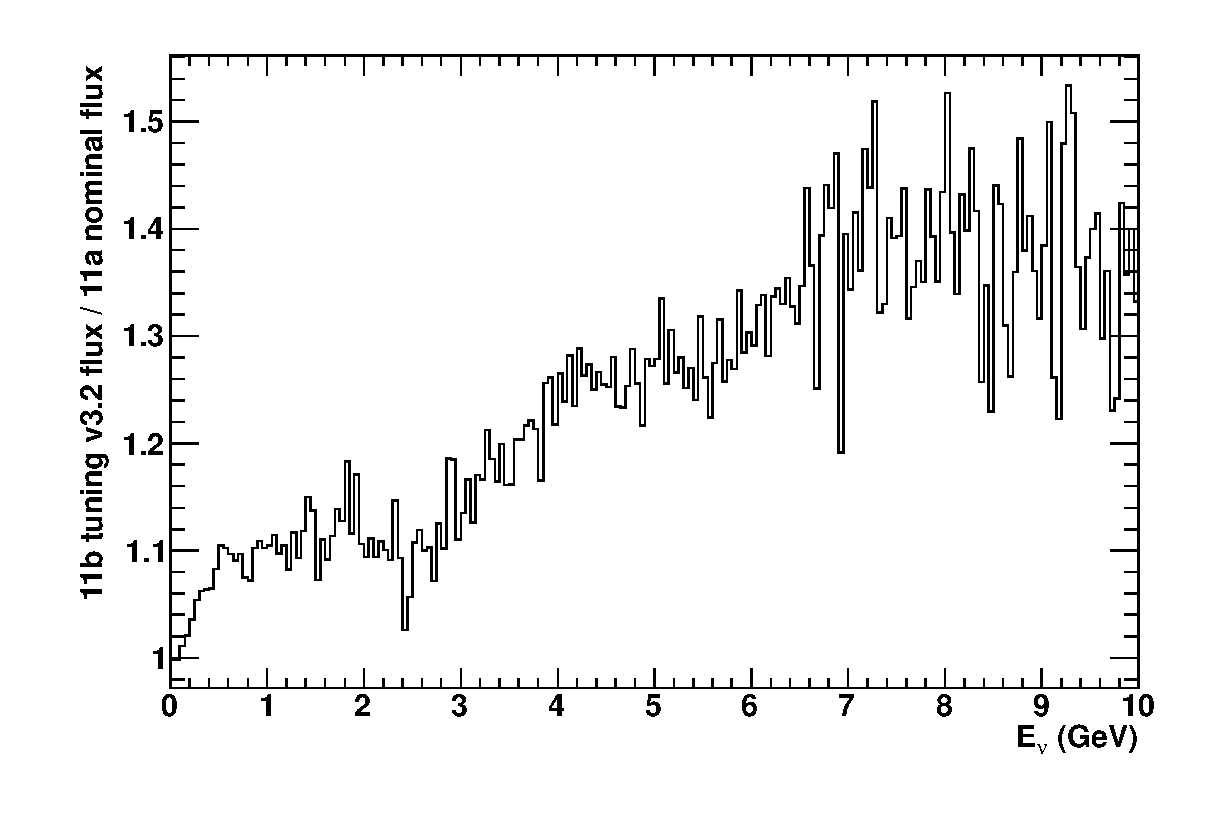
\includegraphics[width=18pc]{./images/fluxtune/fluxtune_numu}
\caption {
  $\nu_\mu$ 2011b\_v3.2\_run1-3c flux tuning weights applied to nominal $\nu_\mu$ and oscillated-$\nu_e$ MC templates.}
\label{fig:na61_weights:numu}
\end{minipage}
\hspace{0.06\linewidth}
\begin{minipage}[t]{0.48\linewidth}
\center
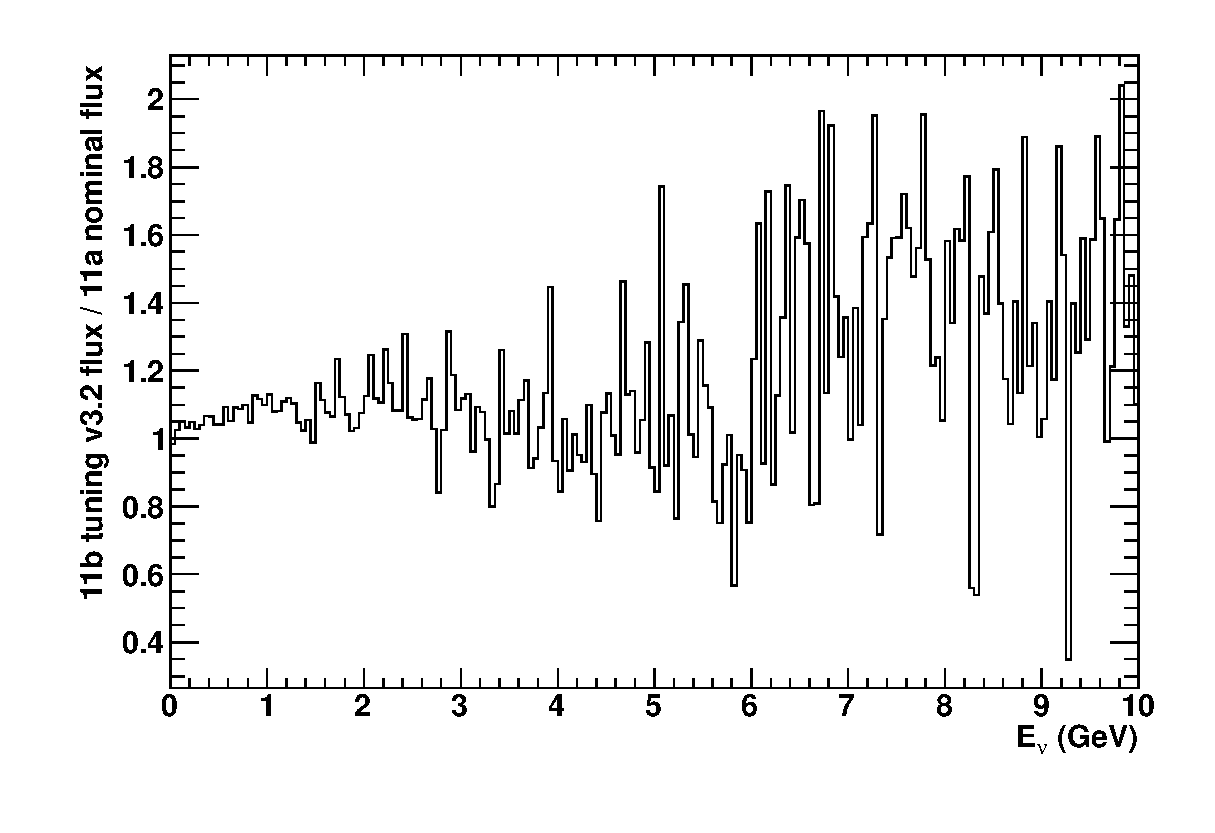
\includegraphics[width=18pc]{./images/fluxtune/fluxtune_numub}
\caption {
  $\bar{\nu_\mu}$ 2011b\_v3.2\_run1-3c flux tuning weights applied to nominal $\bar{\nu_\mu}$ MC templates.}
\label{fig:na61_weights:numubar}
\end{minipage}
\vfill
\begin{minipage}[t]{0.48\linewidth}
\center
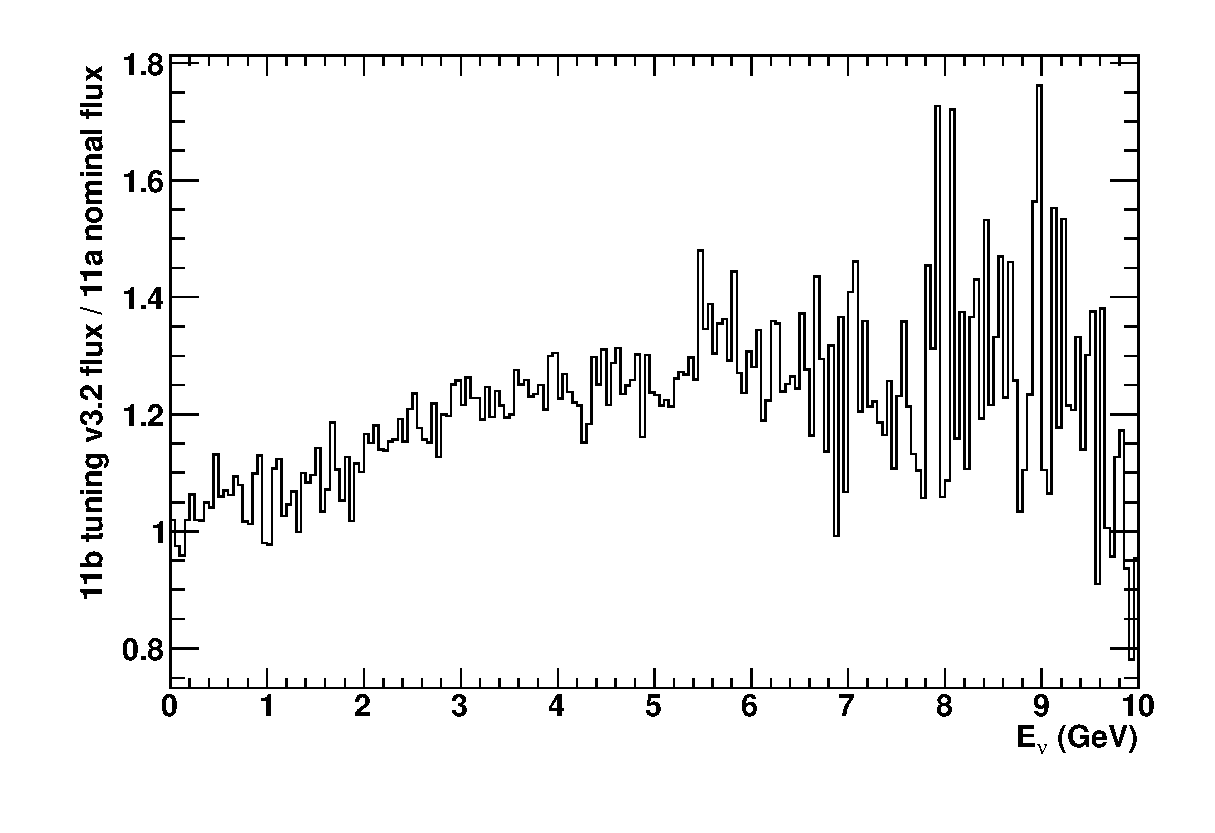
\includegraphics[width=18pc]{./images/fluxtune/fluxtune_nue}
\caption {
  $\nu_e$ 2011b\_v3.2\_run1-3c flux tuning weights applied to nominal $\nu_e$ MC templates.}
\label{fig:na61_weights:nue}
\end{minipage}
\hspace{0.06\linewidth}
\begin{minipage}[t]{0.48\linewidth}
\center
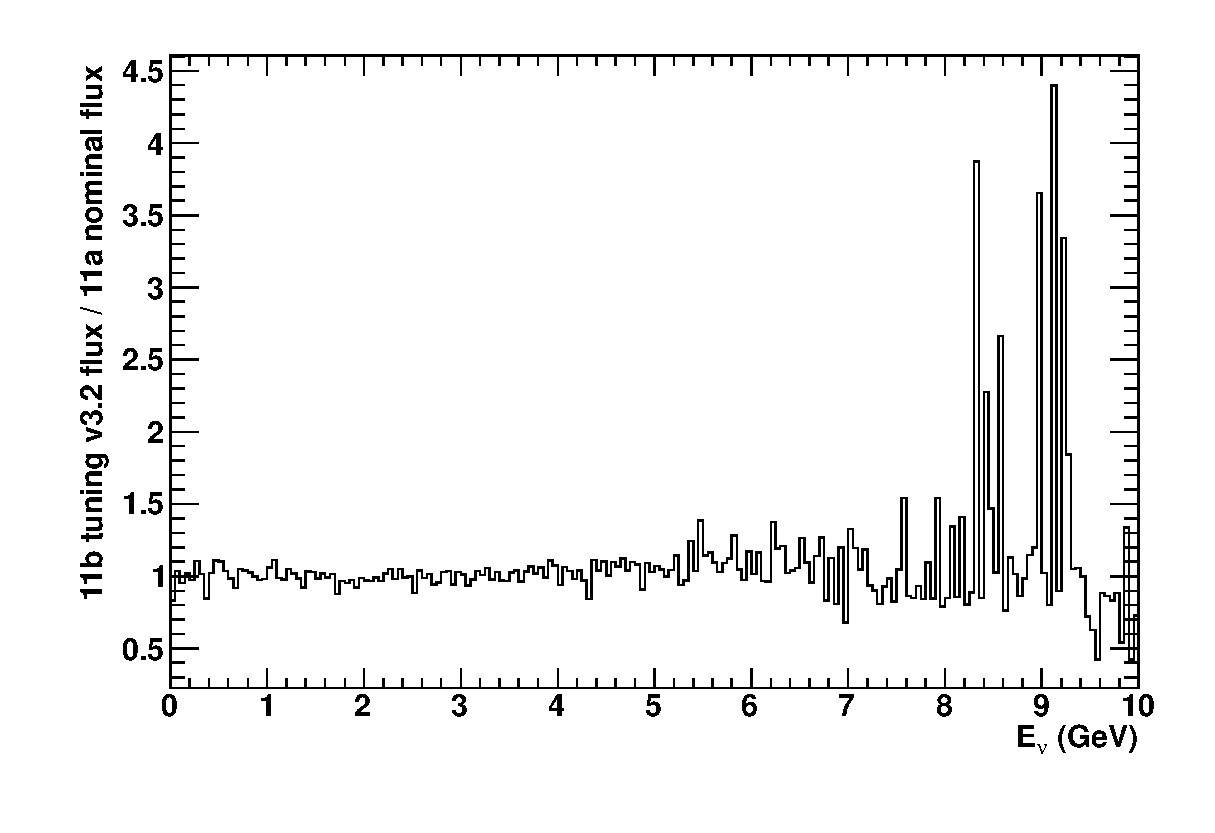
\includegraphics[width=18pc]{./images/fluxtune/fluxtune_nueb}
\caption {
  $\bar{\nu_e}$ 2011b\_v3.2\_run1-3c flux tuning weights applied to nominal $\bar{\nu_e}$ MC templates.}
\label{fig:na61_weights:nuebar}
\end{minipage}
\end{figure*}

%....................................................................................................................
%....................................................................................................................

\subsection {Applying flux and cross-section (BANFF) tuning based on ND280 data}
\label{sec:banff_weights}

This analysis uses the flux and cross-section parameter tuning performed by the 
beam and ND280 flux extrapolation task force (BANFF). 
The BANFF fit combines constraints on the beam flux from the beam monitors and NA61, 
constraints on interaction cross sections from external data (e.g.\ MiniBooNE) and ND280 
measurements of $\nu_\mu$ CCQE-like and CCnonQE-like events with vertices in the FGD fiducial volume.
This fit provides estimates of flux and cross-section parameters 
and their correlations; it also reduces the uncertainties in parameters that are expected to have 
some cancellation between the ND280 and SuperK compared with their uncertainties from external data.
Version 8 of the BANFF fit is used in this analysis \cite{BANFF}.
A list of BANFF parameters and their best-fit values is shown in Tab.\ \ref{tab:banff_params}.

This analysis reweights the NA61-tuned MC templates to the BANFF best-fit parameters
\footnote{
  The BANFF group performed its fit using an NA61-tuned flux ({\em 2011b\_v3.2\_run1-3c}),
  the same one used for reweighting our nominal MC templates in Sec.\ \ref{sec:na61_weights}.
}
\footnote{
  Reweighting the MC templates to the BANFF best-fit parameters is, in effect, a ``special''
  systematic variation. Therefore, more details on 
  are presented in the section detailing the systematic parameters considered in this analysis
  (Sec.\ \ref{sec:systematics}).
}.
The MC templates obtained are referred to, in this document, as the {\em BANFF-tuned} MC templates.
The effect of the BANFF tune on the predicted reconstructed energy spectrum of
single $\mu$-like ring events is discussed in Sec.\ \ref{sec:nominal_and_tuned_predictions} (see 
Figs.\ \ref{fig:nsk_vs_osc_params_effect_of_banff_tune} and \ref{fig:1Rmu_spectrum_w_and_wo_banff_weights}, and
Tabs.\ \ref{tab:nsk_nominal_x3_no_osc} and \ref{tab:nsk_nominal_x3_default_osc}).

%....................................................................................................................
%....................................................................................................................

\subsection{Applying neutrino oscillations}
\label{sec:applying_oscillations}

Oscillation probabilities are computed in a 3-flavour framework including matter effects in constant density matter
(assuming an Earth crust density of 2.6 g/cm$^{3}$).
Custom oscillation probability calculation code was developed within the VaLOR analysis framework.
Details and estimates of the numerical accuracy of this code were first presented in \cite{OurRun12DisappAnalysis3Flavour} 
and, for completeness of the present VaLOR analysis paper, they are given again 
in Appendix \ref{appendix:valor_3f_osc_prob_code}.
Comparisons between the VaLOR oscillation probability calculation code and Prob3++ \cite{Prob3}, 
which is typically used by the alternative T2K oscillation analyses, are shown in Appendix \ref{appendix:comparison_with_prob3}.

Oscillations are applied as a function of true energy to the 
  $\nu_{\mu}$ CCQE,
  $\nu_{\mu}$ CC1$\pi$, 
  $\nu_{\mu}$ CC coherent, 
  $\nu_{\mu}$ CC other, 
  $\bar{\nu}_{\mu}$ CCQE, 
  $\bar{\nu}_{\mu}$ CC1$\pi$, 
  $\bar{\nu}_{\mu}$ CC coherent, 
  $\bar{\nu}_{\mu}$ CC other, 
  $\nu_{e}$ CCQE, 
  $\nu_{e}$ CC1$\pi$,
  $\nu_{e}$ CC coherent,
  $\nu_{e}$ CC other,
  $\bar{\nu}_{e}$ CCQE, 
  $\bar{\nu}_{e}$ CC1$\pi$,
  $\bar{\nu}_{e}$ CC coherent,
  $\bar{\nu}_{e}$ CC other,
  oscillated $\nu_{e}$ CCQE, 
  oscillated $\nu_{e}$ CC1$\pi$,
  oscillated $\nu_{e}$ CC coherent and
  oscillated $\nu_{e}$ CC other
MC templates.

The MC templates constructed from the unoscillated MC samples are weighted 
with the corresponding survival probability:
The $\nu_{\mu}$ templates are weighted with P($\nu_{\mu}\rightarrow\nu_{\mu}$),
the $\bar{\nu}_{\mu}$ templates with P($\bar{\nu}_{\mu}\rightarrow\bar{\nu}_{\mu}$),
the $\nu_{e}$ templates with P($\nu_{e}\rightarrow\nu_{e}$) and
the $\bar{\nu}_{e}$ templates with P($\bar{\nu}_{e}\rightarrow\bar{\nu}_{e}$).
The MC templates made from the oscillated $\nu_{e}$ MC sample are weighted with 
P($\nu_{\mu}\rightarrow\nu_{e}$) (the sample was generated assuming 100\% of 
$\nu_{\mu}$ oscillate to $\nu_{e}$).

We neglect contributions from $\nu_{\tau}$-CC and $\bar{\nu}_{\tau}$-CC as their
energy threshold is around 3.5 GeV and their effect is negligible.

The same $\sin^{2}{2\theta_{23}}$ and $|\Delta m^{2}_{32}|$ parameters 
are used for both $\nu_{\mu}$ and $\bar{\nu_{\mu}}$ oscillations.

Oscillations are not applied to the NC MC templates
  $\nu_{\mu}$ NC1$\pi^{\pm}$, 
  $\nu_{\mu}$ NC other, 
  $\bar{\nu}_{\mu}$ NC1$\pi^{\pm}$, 
  $\bar{\nu}_{\mu}$ NC other, 
  $\nu_{e}$ NC1$\pi^{\pm}$,
  $\nu_{e}$ NC other,
  $\bar{\nu}_{e}$ NC1$\pi^{\pm}$,
  $\bar{\nu}_{e}$ NC other
since, as explained in Sec.\ \ref{sec:mc_templates:template_list}, they serve as proxies for the mixtures of 
$\nu_{e}+\nu_{\mu}+\nu_{\tau}$ NC and 
$\bar{\nu}_{e}+\bar{\nu}_{\mu}+\bar{\nu}_{\tau}$ NC MC templates
which are unchanged under 3-flavour oscillations.


%....................................................................................................................

\subsection {Nominal and tuned-MC single $\mu$-like ring spectrum predictions}
\label{sec:nominal_and_tuned_predictions}

In this section, we present the expected numbers of events and single $\mu$-like ring 
reconstructed energy spectra in SuperK for various oscillation scenarios.
We also present estimates of the effect of the NA61 and BANFF tunings and of assumptions made in the 3-flavour 
neutrino oscillation framework used in this analysis.
Unless explicitly stated otherwise, the normal hierarchy is assumed, 2012 PDG values
are used for $\sin^{2}2\theta_{13}$, $\sin^{2}2\theta_{12}$ and $\Delta m^{2}_{21}$ 
and $\delta_{CP}$=0.
All plots were generated for an integrated exposure of 3.010$\times$10$^{20}$ POT.

The expected number of single $\mu$-like ring events is shown in Fig.\ \ref{fig:nsk_vs_osc_params_tuned_mc}
as a function of the oscillation parameters $\sin^{2}{2\theta_{23}}$ and $|\Delta m^{2}_{32}|$.
The expected number of events ranges from $\sim$58.5
at maximal mixing and at the 2012 MINOS best-fit $|\Delta m^{2}_{32}|$ (2.39$\times10^{-3}$ $eV^{2}/c^{4}$) \cite{MINOS2012},
to more than $\sim$76 for oscillation parameter values still within the 2012 MINOS 90\% confidence region.
This illustrates the great sensitivity of T2K in measuring the $\theta_{23}$ mixing angle.

Predicted single $\mu$-like ring SuperK reconstructed energy spectra are shown in 
Fig. \ref{fig:1Rmu_spectrum_and_components_no_osc} for no oscillations, and in
Fig. \ref{fig:1Rmu_spectrum_and_components_default_osc} for oscillations
with $\sin^{2}2\theta_{23}$ = 1.0 and $|\Delta m^{2}_{32}|$ = 2.4$\times10^{-3}$ $eV^{2}/c^{4}$.

MC tunes derived using NA61 and ND280 data are applied to the nominal MC templates as described earlier 
in this section.
In Fig.\ \ref{fig:nsk_vs_osc_params_effect_of_na61_tune}, the fractional difference is shown in 
the expected number of single $\mu$-like ring events, 
as a function of oscillation parameters $\sin^{2}{2\theta_{23}}$ and $|\Delta m^{2}_{32}|$,
obtained when this analysis switches from the nominal MC to the NA61-tuned MC templates. 
The fractional difference in the expected number of single $\mu$-like ring events 
when switching from the NA61-tuned MC templates to the BANFF-tuned MC templates is also shown in 
Fig. \ref{fig:nsk_vs_osc_params_effect_of_banff_tune}. 
From these figures it can be seen that, for oscillation parameters in the 2012 MINOS 90\% confidence region, 
$\sim$11.5-12.5\% more single $\mu$-like ring events are obtained with
the NA61-tuned MC than with the nominal MC.
In the same part of the parameter space, $\sim$1.8-2.0\% fewer events are expected with the BANFF-tuned MC 
than with the NA61-tuned MC.
The effects of the NA61 and BANFF tunes on the total expected number of single $\mu$-like ring events 
and on the numbers in each of the 28 component reaction modes are shown in 
Tab.\ \ref{tab:nsk_nominal_x3_no_osc} for no oscillations, and in
Tab.\ \ref{tab:nsk_nominal_x3_default_osc} for oscillations
with $\sin^{2}2\theta_{23}$ = 1.0 and $|\Delta m^{2}_{32}|$ = 2.4$\times10^{-3}$ $eV^{2}/c^{4}$.
Finally, the effect of the NA61 and BANFF tunes on the reconstructed energy spectrum of
single $\mu$-like ring events is shown in Figs.\
\ref{fig:1Rmu_spectrum_w_and_wo_na61_weights} and
\ref{fig:1Rmu_spectrum_w_and_wo_banff_weights} respectively. 
In each case, spectra are shown for both no oscillations and for
oscillations with $\sin^{2}2\theta_{23}$ = 1.0 and $|\Delta m^{2}_{32}|$ = 2.4$\times10^{-3}$ $eV^{2}/c^{4}$.

The effect of the choice of octant of $\theta_{23}$ \footnote{
  It should be noted that, in the earlier versions of this note, the first octant ($\sin(\theta) \leq 0.5$) was assumed for all the PMNS oscillation angles. 
In this version, the first octant is assumed for all mixing angles unless explicitly stated otherwise.
The octant choice does however make a difference;
by making some approximations to the 3-flavour P($\nu_{\mu}\rightarrow\nu_{\mu}$) formula % in equation \ref{eq:numusurv3f}. 
%(setting $\Delta m_{32}^{2}$ = $\Delta m_{31}^{2}$, and neglecting $\Delta m_{21}^{2}$ and the third terms in both $|U_{\mu 1}|^{2}$ and $|U_{\mu 2}|^{2}$,
%and assuming vacuum oscillations), %Lorena
(neglecting $\sin^2\left(\frac{\Delta m^2_{21} L}{4E}\right)$ and $\sin^2\left(\frac{2 \Delta m^2_{31} L}{4E}\right)$), %Minamino-san
we get
\begin{equation}
  P(\nu_{\mu}\rightarrow\nu_{\mu})
  \approx 1 - \left( \cos^4(\theta_{13})\sin^2(2\theta_{23}) + \sin^2(\theta_{23})\sin^2(2\theta_{13}) \right) \sin^2\left(\frac{\Delta m_{31}^{2} L}{4E}\right). %Minamino-san
  %\approx 1 - \left( \cos^2(\theta_{13})\sin^2(2\theta_{23}) + \sin^4(\theta_{23})\sin^2(2\theta_{13}) \right) \sin^2\left(\frac{\Delta m_{31}^{2} L}{4E}\right). %Lorena
  \label{eqn:numusurv3fapprox}
\end{equation}
The minimum of Eq.\ \ref{eqn:numusurv3fapprox} occurs at
\begin{equation}
  \sin^2(\theta_{23})
  = \frac{1}{2(1-\sin^2(\theta_{13}))},
  \label{eqn:numusurv3fmin}
\end{equation}
and so, when $\theta_{13} \ne 0$, moves from $\sin^2(\theta_{23}) = 0.5$ to $\sin^2(\theta_{23}) > 0.5$.
More discussion of this effect can be found in Appendix E of \cite{OurRun123JointOscillationAnalysis}.
It should be noted that when $\sin^2(2\theta_{23}) = 1.000$, the oscillation probability is identical,
no matter the value of $\theta_{13}$, and no matter which octant is chosen.
For both $\sin^2(\theta_{12})$ and $\sin^2(\theta_{13})$ we always assume the first octant.
} on the energy spectrum of
single $\mu$-like ring events is shown in Fig.\
\ref{fig:1Rmu_spectrum_octant_comparison}, for oscillations with
$\sin^{2}2\theta_{23}$ = 0.95 (the 2012 PDG 90\% lower limit) and
$|\Delta m^{2}_{32}|$ = 2.4$\times10^{-3}$ $eV^{2}/c^{4}$.
It follows from Eq.\ \ref{eqn:numusurv3fapprox} that the effect of changing from the first to second octant is 
to increase the depth of the oscillation dip, which is why the spectra are almost identical above the oscillation maximum.
The fractional difference in the total expected number of single $\mu$-like ring events when switching between the first and second octant
is shown in Fig.\ \ref{fig:nsk_vs_osc_params_tuned_mc_effect_of_octant}.

When making a fit to obtain the best-fit values of $\sin^{2}2\theta_{23}$ and $|\Delta m^{2}_{32}|$, we fix the 
non-23 oscillation parameters: $\sin^{2}2\theta_{13}$, $\sin^{2}2\theta_{12}$ $\Delta m^{2}_{21}$ are fixed 
to the 2012 PDG values and $\delta_{CP}$ is fixed to 0 (see Sec.\ \ref{sec:oscfit_method_non23params}). The 
maximum possible effect of this assumption on the expected number of single $\mu$-like ring events is shown 
in Fig.\ \ref{fig:nsk_vs_osc_params_tuned_mc_effect_of_non23}.
In each bin of $\sin^{2}{2\theta_{23}}$ and $|\Delta m^{2}_{32}|$,
a large number of toy MC experiments was generated with randomized values of the non-23 parameters. 
The random values of $\sin^{2}2\theta_{13}$, $\sin^{2}2\theta_{12}$ and $\Delta m^{2}_{21}$ were drawn from 
Gaussian distributions with means equal to the 2012 PDG values and standard deviations equal to the 1$\sigma$ 
errors, while the values of $\delta_{CP}$ were drawn from a uniform distribution between -$\pi$ and +$\pi$.
These four non-23 parameters were taken to be uncorrelated.
The maximum frational deviation from the default case was recorded and plotted 
in Fig.\ \ref{fig:nsk_vs_osc_params_tuned_mc_effect_of_non23}.
From this figure, it can be seen that the effect of the non-23-sector oscillation parameters is small:
the maximum fractional deviation from the default assumption is of the order of $\sim$1\% in the part of 
the parameter space covered by the 2012 MINOS 90\% confidence region. 

All the results in this analysis assume the normal mass hierarchy. 
The effect of this assumption on the expected number of single $\mu$-like ring events
is shown in Fig.\ \ref{fig:nsk_vs_osc_params_tuned_mc_effect_of_hierarchy} 
as a function of the oscillation parameters $\sin^{2}{2\theta_{23}}$ and $|\Delta m^{2}_{32}|$.
The effect is large and potentially misleading, and some clarifications are in order.
This analysis can assume a given hierarchy (in our case, normal) without loss of generality of its results.
Fig.\ \ref{fig:nsk_vs_osc_params_tuned_mc_effect_of_hierarchy} reveals that $|\Delta m^{2}_{32}|$ is a poor 
choice as the atmospheric mass-squared difference when both mass hierarchies need to be considered,
since $|\Delta m^{2}_{32}|$ is the largest mass-squared difference for the inverted hierarchy 
but the second-largest for the normal hierarchy. 
The large difference shown in Fig.\ \ref{fig:nsk_vs_osc_params_tuned_mc_effect_of_hierarchy} 
is caused by the change in value of $\Delta m^{2}_{31}$ when switching from the
normal to inverted hierarchy.

Other choices exist for the atmospheric mass-squared difference, and these are explained in Sec.\ 
\ref{sec:oscfit_method_23param_choice}. An example of an alternative choice is shown vividly in 
Fig.\ 5 in \cite{OurRun12DisappAnalysis3Flavour}; this technical note describes a repeat, in a 3-flavour 
framework, of our official Run1+2 disappearance analysis \cite{OurRun12DisappAnalysis} which was originally 
performed in a 2-flavour framework.

The reader may also be interested in comparisons of oscillated single $\mu$-like ring spectra,
obtained in a 3-flavour framework with spectra obtained in a 2-flavour framework.
Many such comparisons were presented in \cite{OurRun12DisappAnalysis3Flavour}.

%...........
%
% nsk
%
\begin{figure*}[htb]
\center
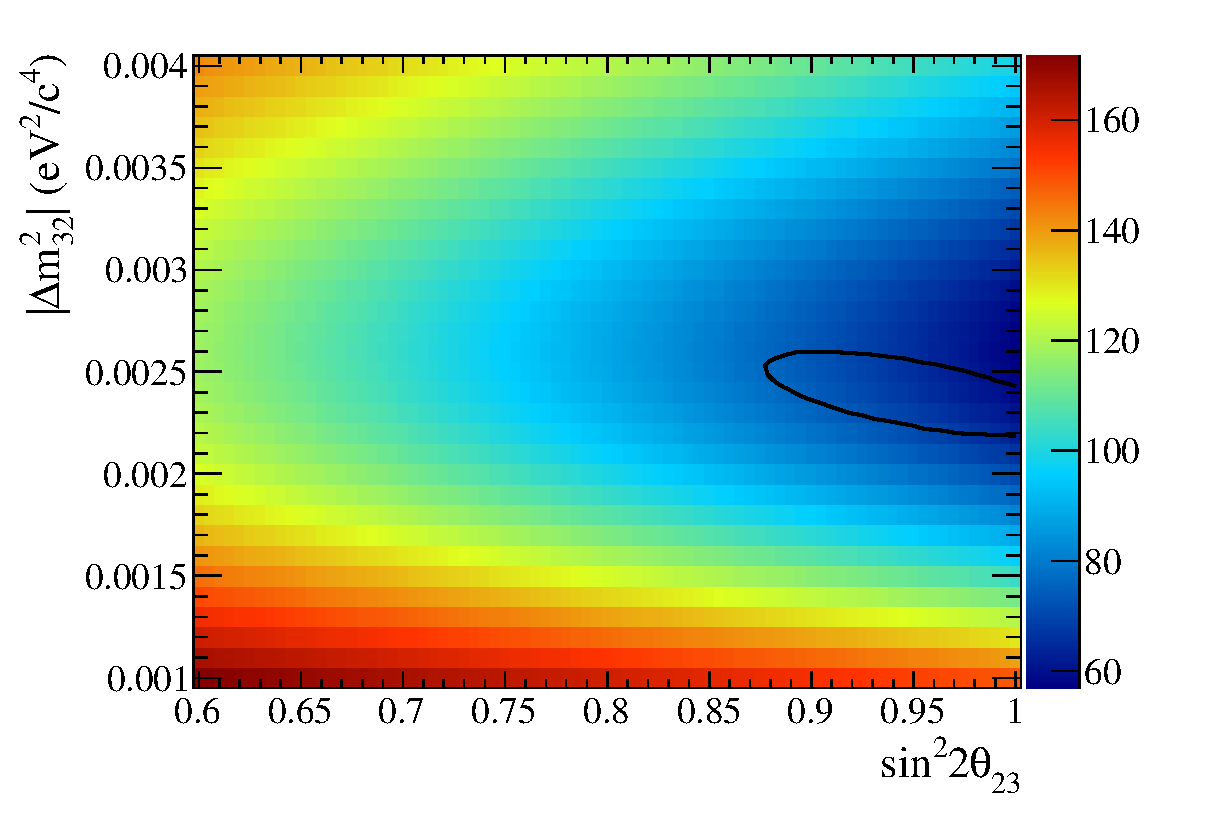
\includegraphics[width=32pc]{./images/spectrum_nominal/nsk_nominalbanff}
\caption {
  Predicted number of 1-ring $\mu$-like events,
  as a function of $\sin^{2}2\theta_{23}$ and $|\Delta m^{2}_{32}|$,
  for an exposure of 3.010$\times$10$^{20}$ POT.
  The number of events was calculated using the BANFF-tuned MC templates.
  2012 PDG values are used for $\sin^{2}2\theta_{13}$, $\sin^{2}2\theta_{12}$ and $\Delta m^{2}_{21}$ and $\delta_{CP}$=0. 
  The numbers shown were generated assuming the normal hierarchy.
  The 2012 MINOS 90\% confidence region is superimposed for reference.
}
\label{fig:nsk_vs_osc_params_tuned_mc}
\end{figure*}

%...........
%
% spectra, various osc scenarios
%
\begin{figure*}[htb]
\begin{minipage}[t]{0.48\linewidth}
\center
\includegraphics[width=20pc]{{./images/spectrum_nominal/sk_ereco_spectrum-0.000000-0.000000-grouped-components}.eps}
\caption {
Predicted reconstructed-energy spectrum of 1-ring $\mu$-like events,
and contributions from various true neutrino reaction modes,
for no oscillations and
for an exposure of 3.010$\times$10$^{20}$ POT.
The 28 components of the spectrum are calculated separately in the actual analysis, 
but, for this plot, are grouped into just 5 categories: 
$\nu_{\mu}$ CCQE, $\nu_{\mu}$ CCnonQE, $\bar{\nu_{\mu}}$ CC, $\nu_{e}$/$\bar{\nu_{e}}$ CC and NC.
The spectrum was generated using the BANFF-tuned MC templates.
}
\label{fig:1Rmu_spectrum_and_components_no_osc}
\end{minipage}
\hspace{0.06\linewidth}
\begin{minipage}[t]{0.48\linewidth}
\center
\includegraphics[width=20pc]{{./images/spectrum_nominal/sk_ereco_spectrum-1.000000-0.002400-grouped-components}.eps}
\caption {
Predicted reconstructed-energy spectrum of 1-ring $\mu$-like events,
and contributions from various true neutrino reaction modes,
for oscillations with $\sin^{2}2\theta_{23}$=1.0 and $|\Delta m^{2}_{32}|$=2.4$\times10^{-3}$ $eV^{2}/c^{4}$ 
and for an exposure of 3.010$\times$10$^{20}$ POT.
The spectrum was generated using the BANFF-tuned MC templates.
2012 PDG values are used for $\sin^{2}2\theta_{13}$, $\sin^{2}2\theta_{12}$ and $\Delta m^{2}_{21}$ and $\delta_{CP}$=0. 
The spectrum shown was generated assuming the normal hierarchy.
Note that the vertical axis is zoomed in by a factor of 4 compared with Fig.\ \ref{fig:1Rmu_spectrum_and_components_no_osc}.
}
\label{fig:1Rmu_spectrum_and_components_default_osc}
\end{minipage}
\end{figure*}

%...........
%
% effect of tunes on nsk
%
\begin{figure*}[htb]
\begin{minipage}[t]{0.48\linewidth}
\center
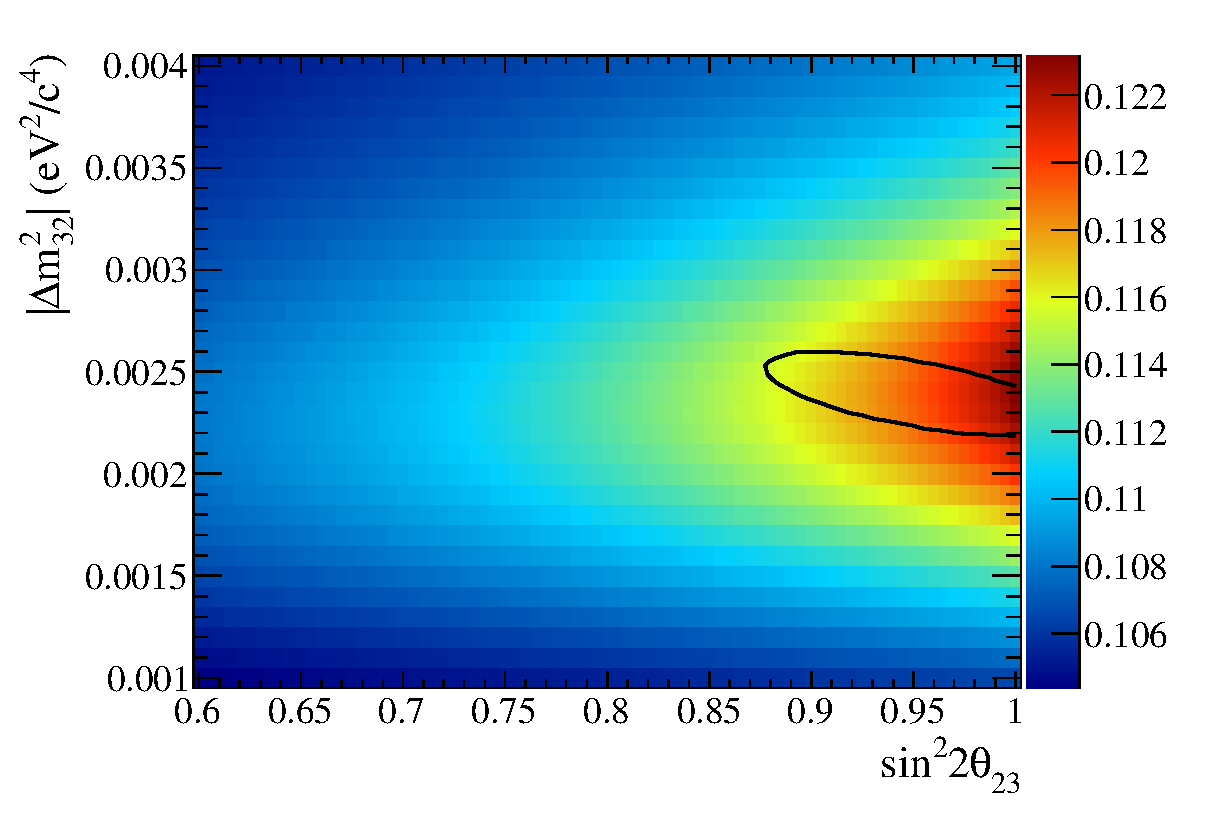
\includegraphics[width=18pc]{./images/spectrum_nominal/nsk_diff_nomflux}
\caption {
  Fractional difference in the predicted number of 1-ring $\mu$-like events 
  as a result of applying the 2011b v3.2 flux tuning to the nominal MC templates.
  This number is shown as a function of $\sin^{2}2\theta_{23}$ and $|\Delta m^{2}_{32}|$
  for an exposure of 3.010$\times$10$^{20}$ POT.
  The 2012 PDG parameters are used for $\sin^{2}2\theta_{13}$, $\sin^{2}2\theta_{12}$ and $\Delta m^{2}_{21}$,and $\delta_{CP}$=0. 
  The numbers shown were generated assuming the normal hierarchy.
  The MINOS 2012 90\% CL region is superimposed for reference.
}
\label{fig:nsk_vs_osc_params_effect_of_na61_tune}
\end{minipage}
\hspace{0.06\linewidth}
\begin{minipage}[t]{0.48\linewidth}
\center
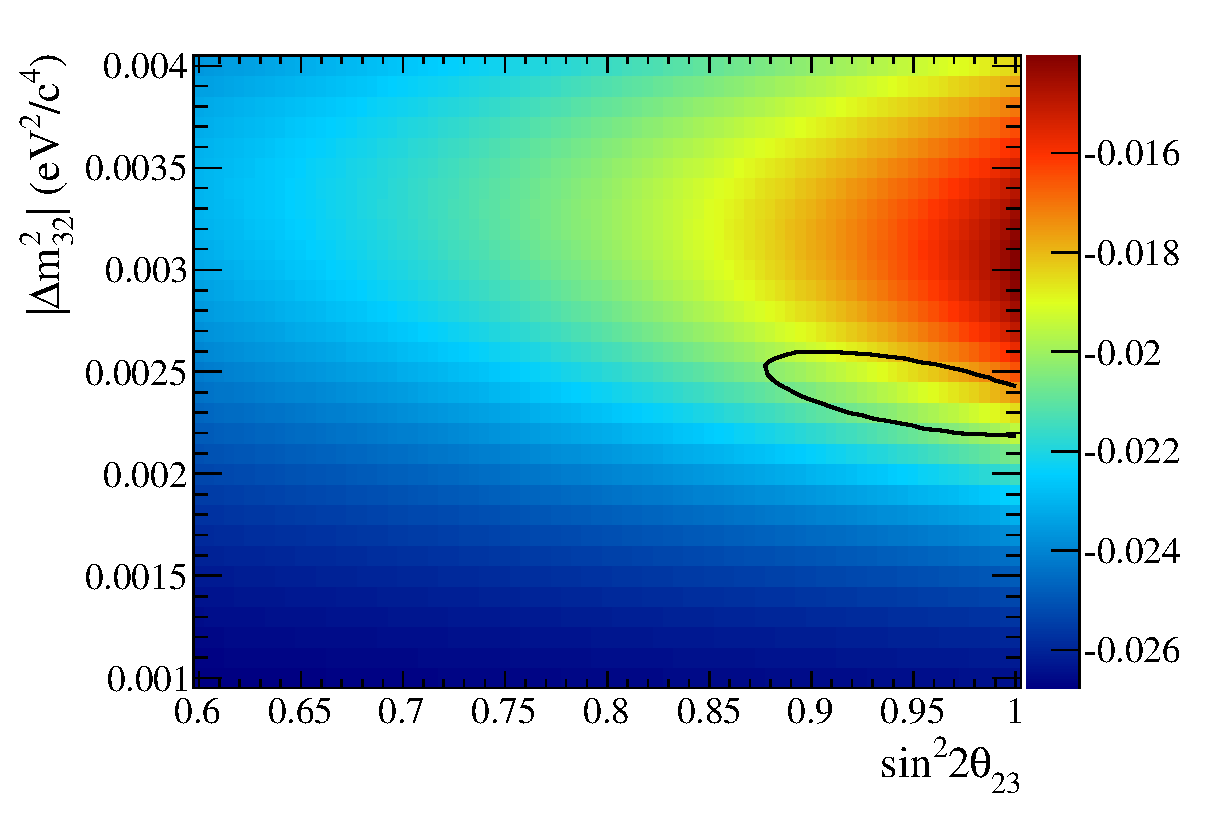
\includegraphics[width=18pc]{./images/spectrum_nominal/nsk_diff_tunflux}
\caption {
  Fractional difference in the predicted number of 1-ring $\mu$-like events
  as a result of applying the BANFF flux and cross-section tuning to the 2011b v3.2 flux tuned MC templates.
  This number is shown as a function of $\sin^{2}2\theta_{23}$ and $|\Delta m^{2}_{32}|$ and 
  for an exposure of 3.010$\times$10$^{20}$ POT.
  The 2012 PDG values are used for $\sin^{2}2\theta_{13}$, $\sin^{2}2\theta_{12}$ and $\Delta m^{2}_{21}$, and $\delta_{CP}$=0. 
  The numbers shown were generated assuming the normal hierarchy.
  The MINOS 2012 90\% CL region is superimposed for reference.
}
\label{fig:nsk_vs_osc_params_effect_of_banff_tune}
\end{minipage}
\end{figure*}


%...........
%
% tables showing the effect of tunes on nsk and nsk components
%
\begin{table}
\centering
\begin{tabular}{| c | c | c | c | }
\hline
       & $N_{SK}$     & $N_{SK}$         & $N_{SK}$                      \\
       & (nominal MC) & (NA61-tuned MC)  & (BANFF-tuned MC)  \\
\hline
Total & 190.986142 & 210.464599 &  204.747590 \\
\hline
$\nu_\mu$ CCQE &      151.820154 & 166.353705 & 155.044970 \\
$\nu_\mu$ CC 1$\pi$ &       25.717606 & 28.879686 & 34.945661 \\
$\nu_\mu$ CC coherent &        0.898432 & 1.005621 & 0.950276 \\
$\nu_\mu$ CC other &        3.584984 & 4.315475 & 4.198557 \\
$\nu_\mu$/$\nu_\tau$ NC 1$\pi^{+/-}$ &        1.492903 & 1.696744 & 1.625483 \\
$\nu_\mu$/$\nu_\tau$ NC other &        1.294522 & 1.521644 & 1.466497 \\
$\bar{\nu}_{\mu}$ CCQE &        4.118572 & 4.459811 & 3.981437 \\
$\bar{\nu}_{\mu}$ CC 1$\pi$ &        1.336699 & 1.445418 & 1.762408 \\
$\bar{\nu}_{\mu}$ CC coherent &        0.194978 & 0.211123 & 0.202799 \\
$\bar{\nu}_{\mu}$ CC other &        0.236537 & 0.253912 & 0.247794 \\
$\bar{\nu}_{\mu}$/$\bar{\nu}_{\tau}$ NC 1$\pi^{+/-}$ &        0.084582 & 0.091984 & 0.090422 \\
$\bar{\nu}_{\mu}$/$\bar{\nu}_{\tau}$ NC other &        0.073460 & 0.079580 & 0.077614 \\
$\nu_e$ CCQE &        0.015774 & 0.016972 & 0.016260 \\
$\nu_e$ CC 1$\pi$ &        0.009050 & 0.009932 & 0.013125 \\
$\nu_e$ CC coherent &        0.000403 & 0.000434 & 0.000434 \\
$\nu_e$ CC other &        0.002568 & 0.003048 & 0.003051 \\
$\nu_e$ NC 1$\pi^{+/-}$ &        0.042494 & 0.048652 & 0.049421 \\
$\nu_e$ NC other &        0.049084 & 0.057414 & 0.057684 \\
$\bar{\nu}_{e}$ CCQE &        0.000822 & 0.000827 & 0.000790 \\
$\bar{\nu}_{e}$ CC 1$\pi$ &        0.000599 & 0.000601 & 0.000745 \\
$\bar{\nu}_{e}$ CC coherent &        0.000073 & 0.000073 & 0.000073 \\
$\bar{\nu}_{e}$ CC other &        0.000214 & 0.000219 & 0.000219 \\
$\bar{\nu}_{e}$ NC 1$\pi^{+/-}$ &        0.005755 & 0.005805 & 0.005916 \\
$\bar{\nu}_{e}$ NC other &        0.005876 & 0.005918 & 0.005954 \\
Oscillated $\nu_e$ CCQE &        0.000000 & 0.000000 & 0.000000 \\
Oscillated $\nu_e$ CC 1$\pi$ &        0.000000 & 0.000000 & 0.000000 \\
Oscillated $\nu_e$ CC coherent &        0.000000 & 0.000000 & 0.000000 \\
Oscillated $\nu_e$ CC other &        0.000000 & 0.000000 & 0.000000 \\
\hline
\end{tabular}
\caption{
  Calculated numbers of 1-ring $\mu$-like events without oscillations using the nominal MC templates, the 
  NA61-tuned MC templates and the BANFF-tuned MC templates.
  The total numbers of events and the numbers of events from each mode considered in this analysis are shown.
  These numbers were calculated for an exposure of 3.010$\times$10$^{20}$ POT.
}
\label{tab:nsk_nominal_x3_no_osc}
\end{table}


\begin{table}
\centering
\begin{tabular}{| c | c | c | c | }
\hline
       & $N_{SK}$     & $N_{SK}$              & $N_{SK}$                      \\
       & (nominal MC) & (NA61-tuned MC)  & (BANFF-tuned MC)  \\
\hline
Total & 52.890886 & 59.406174 & 58.367775 \\
\hline
$\nu_\mu$ CCQE &       30.122383 & 33.277415 & 30.285520 \\
$\nu_\mu$ CC 1$\pi$ &       12.736216 & 14.628739 & 16.931486 \\
$\nu_\mu$ CC coherent &        0.365047 & 0.420613 & 0.399710 \\
$\nu_\mu$ CC other &        3.187277 & 3.862403 & 3.771051 \\
$\nu_\mu$/$\nu_\tau$ NC 1$\pi^{+/-}$ &        1.492903 & 1.696744 & 1.625483 \\
$\nu_\mu$/$\nu_\tau$ NC other &        1.294522 & 1.521644 & 1.466497 \\
$\bar{\nu}_{\mu}$ CCQE &        2.023300 & 2.190691 & 1.891082 \\
$\bar{\nu}_{\mu}$ CC 1$\pi$ &        0.958303 & 1.032827 & 1.228001 \\
$\bar{\nu}_{\mu}$ CC coherent &        0.104487 & 0.112894 & 0.108444 \\
$\bar{\nu}_{\mu}$ CC other &        0.209999 & 0.225107 & 0.220043 \\
$\bar{\nu}_{\mu}$/$\bar{\nu}_{\tau}$ NC 1$\pi^{+/-}$ &        0.084582 & 0.091984 & 0.090422 \\
$\bar{\nu}_{\mu}$/$\bar{\nu}_{\tau}$ NC other &        0.073460 & 0.079580 & 0.077614 \\
$\nu_e$ CCQE &        0.014633 & 0.015752 & 0.015068 \\
$\nu_e$ CC 1$\pi$ &        0.008572 & 0.009421 & 0.012426 \\
$\nu_e$ CC coherent &        0.000375 & 0.000404 & 0.000404 \\
$\nu_e$ CC other &        0.002530 & 0.003005 & 0.003007 \\
$\nu_e$ NC 1$\pi^{+/-}$ &        0.042494 & 0.048652 & 0.049421 \\
$\nu_e$ NC other &        0.049084 & 0.057414 & 0.057684 \\
$\bar{\nu}_{e}$ CCQE &        0.000785 & 0.000790 & 0.000755 \\
$\bar{\nu}_{e}$ CC 1$\pi$ &        0.000583 & 0.000585 & 0.000724 \\
$\bar{\nu}_{e}$ CC coherent &        0.000070 & 0.000070 & 0.000070 \\
$\bar{\nu}_{e}$ CC other &        0.000212 & 0.000217 & 0.000217 \\
$\bar{\nu}_{e}$ NC 1$\pi^{+/-}$ &        0.005755 & 0.005805 & 0.005916 \\
$\bar{\nu}_{e}$ NC other &        0.005876 & 0.005918 & 0.005954 \\
Oscillated $\nu_e$ CCQE &        0.079970 & 0.087419 & 0.082883 \\
Oscillated $\nu_e$ CC 1$\pi$ &        0.024965 & 0.027318 & 0.035271 \\
Oscillated $\nu_e$ CC coherent &        0.001860 & 0.002039 & 0.001949 \\
Oscillated $\nu_e$ CC other &        0.000644 & 0.000723 & 0.000672 \\
\hline
\end{tabular}
\caption{
  Calculated numbers of 1-ring $\mu$-like events using the nominal MC templates, the NA61-tuned MC templates
  and the BANFF-tuned MC templates.
  The total numbers of events and the numbers of events from each mode considered in this analysis are shown.
  These numbers were calculated for an exposure of 3.010$\times$10$^{20}$ POT
  and oscillations with $\sin^{2}2\theta_{23}$=1.0 and $|\Delta m^{2}_{32}|$=2.4$\times10^{-3}$ $eV^{2}/c^{4}$.
  The 2012 PDG parameters are used for $\sin^{2}2\theta_{13}$, $\sin^{2}2\theta_{12}$ and $\Delta m^{2}_{21}$ and $\delta_{CP}$=0. 
  The normal hierarchy is assumed.
}
\label{tab:nsk_nominal_x3_default_osc}
\end{table}

%...........
%
% Plots showing the effect of tunes on Ereco spectra
%
\begin{figure*}[htb]
\center
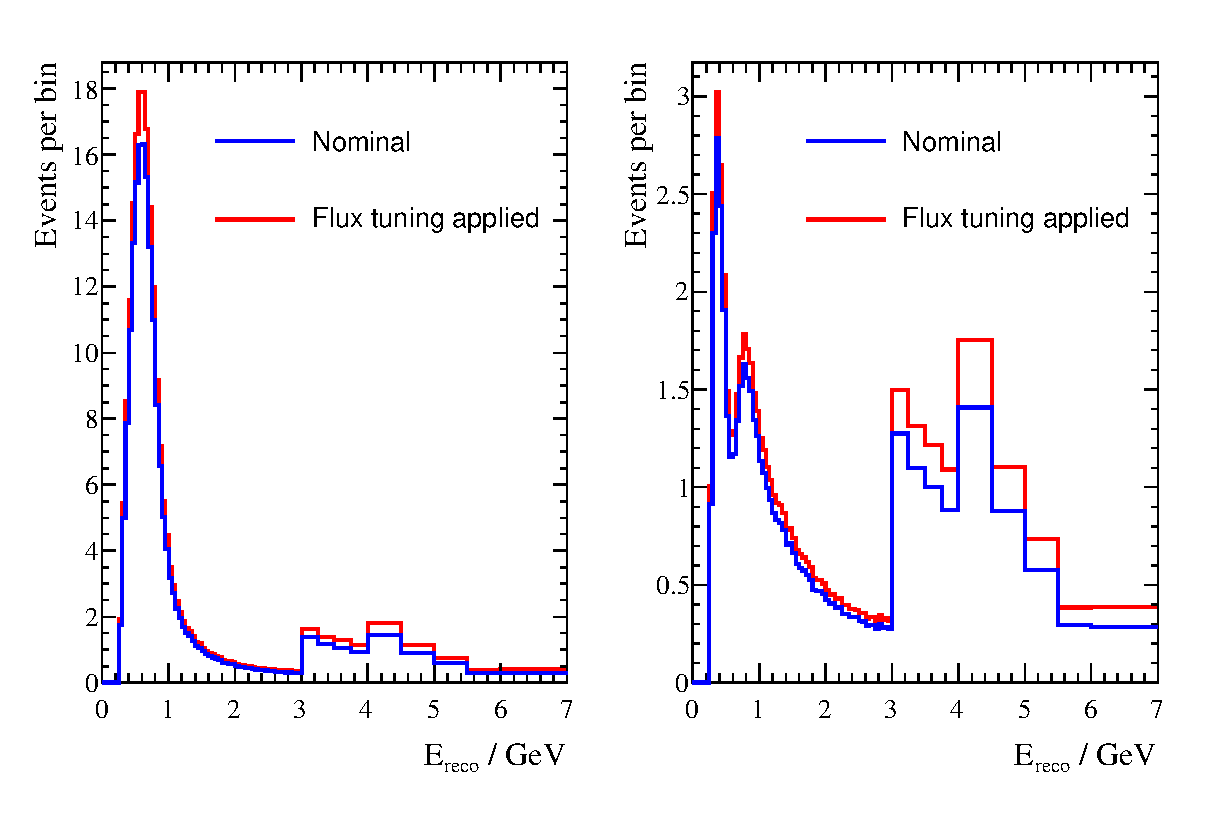
\includegraphics[width=30pc]{./images/spectrum_nominal/spectra_nom_fluxtuned}
\caption {
Reconstructed-energy spectrum of 1-ring $\mu$-like events, 
for an exposure of 3.010$\times$10$^{20}$ POT,
both with and without the effect of the {\em 2011b\_v3.2\_run1-3c} flux tuning of the nominal MC templates. 
The spectra are shown both for no oscillations (left) 
and for oscillations with $\sin^{2}2\theta_{23}$=1.0, $|\Delta m^{2}_{32}|$=2.4$\times10^{-3}$ $eV^{2}/c^{4}$, 
the 2012 PDG values for $\sin^{2}2\theta_{13}$, $\sin^{2}2\theta_{12}$ and $\Delta m^{2}_{21}$, and 
$\delta_{CP}$=0 (right). Results shown for the normal hierarchy.
}
\label{fig:1Rmu_spectrum_w_and_wo_na61_weights}
\end{figure*}

\begin{figure*}[htb]
\center
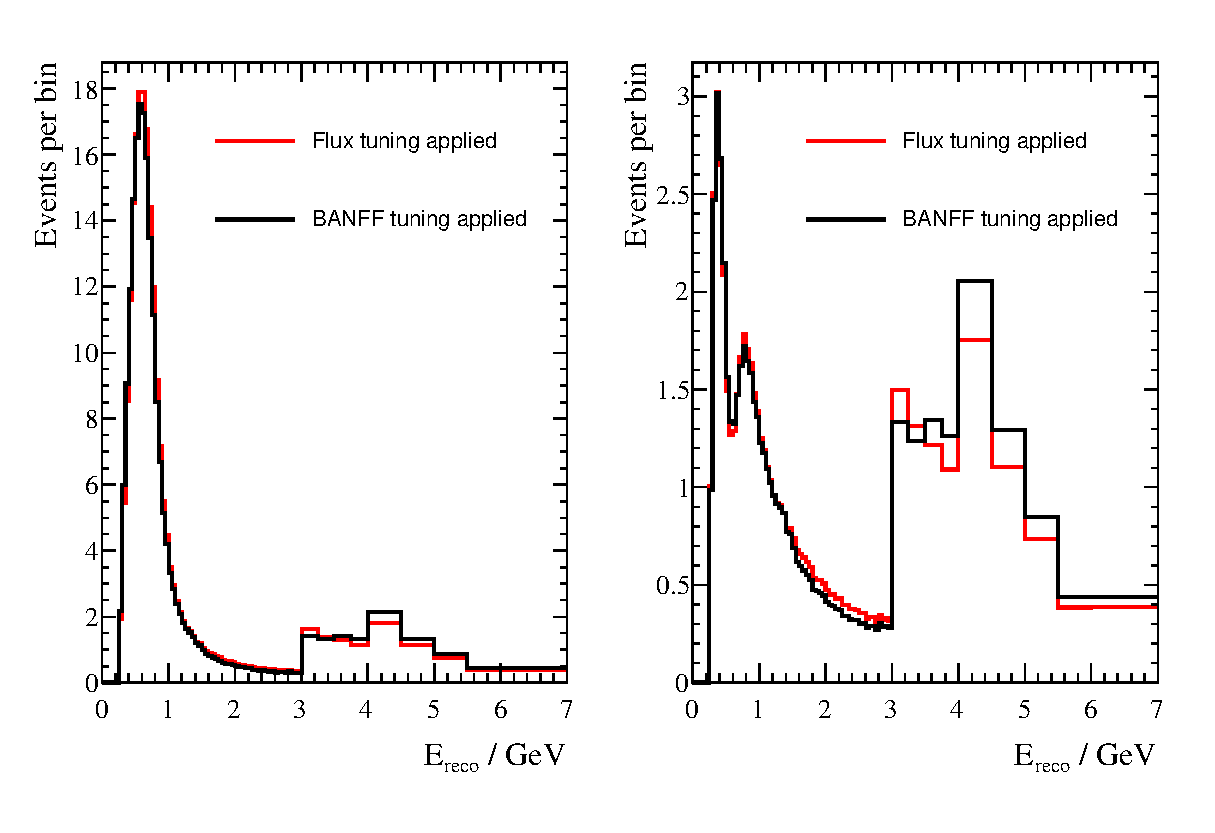
\includegraphics[width=30pc]{./images/spectrum_nominal/spectra_tun_banfftuned}
\caption {
Reconstructed-energy spectrum of 1-ring $\mu$-like events,
for an exposure of 3.010$\times$10$^{20}$ POT,
both with and without the effect of BANFF flux and cross-section tuning on the NA61-tuned {\em 2011b\_v3.2\_run1-3c} flux MC templates.
The spectra are shown both for no 23-sector oscillations (left) 
and for oscillations with $\sin^{2}2\theta_{23}$=1.0 and $|\Delta m^{2}_{32}|$=2.4$\times10^{-3}$ $eV^{2}/c^{4}$ (right).
In all spectra, the 2012 PDG parameters are used for $\sin^{2}2\theta_{13}$, $\sin^{2}2\theta_{12}$ and $\Delta m^{2}_{21}$
and $\delta_{CP}$=0. Results shown for the normal hierarchy.
}
\label{fig:1Rmu_spectrum_w_and_wo_banff_weights}
\end{figure*}

% ...........
%
% effect of octant on spectrum
% effect of octant on Nsk
%
\begin{figure*}[htb]
\begin{minipage}[t]{0.48\linewidth}
\center
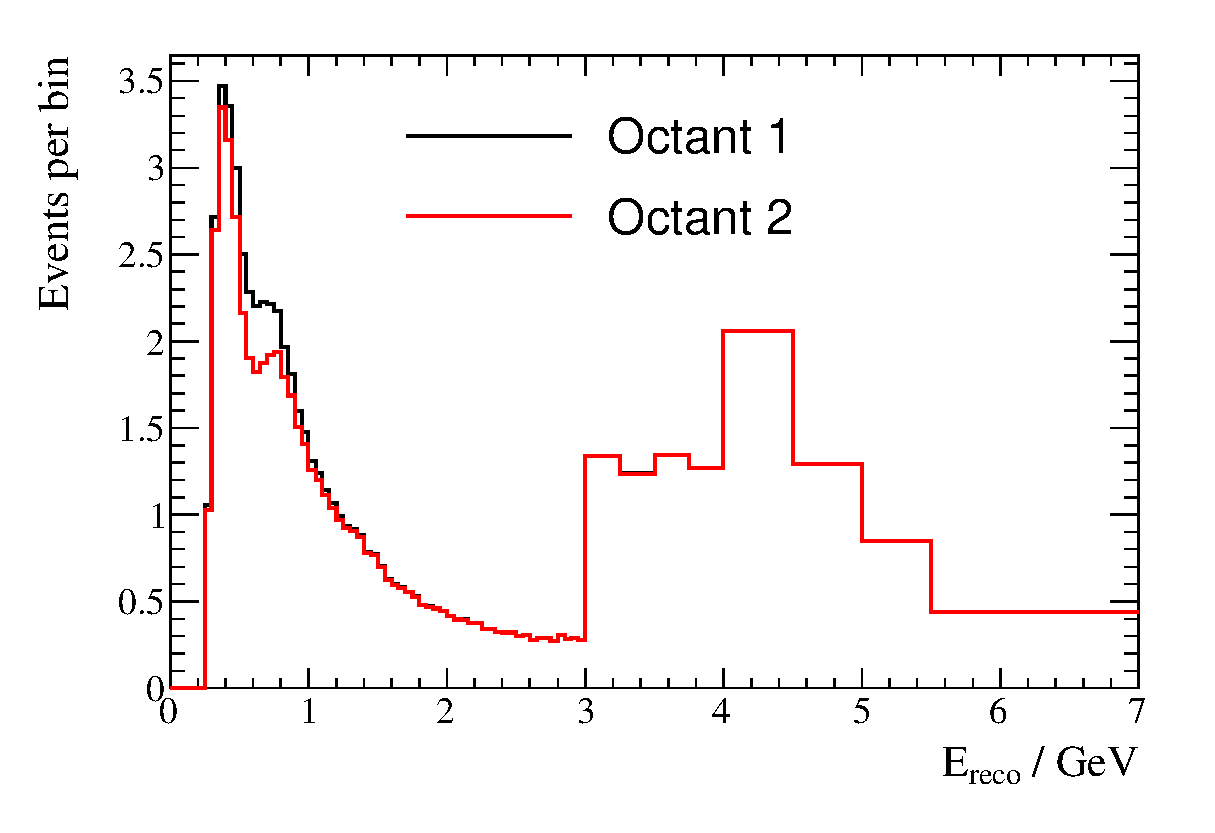
\includegraphics[width=18pc]{./images/spectrum_nominal/spectra_octants}
\caption {
  Predicted reconstructed-energy spectrum of 1-ring $\mu$-like events, 
  for an exposure of 3.010$\times$10$^{20}$ POT,
  for $\theta_{23}$ both in the first octant and second octant. 
  The spectra are shown oscillations with $\sin^{2}2\theta_{23}$=0.95, $|\Delta m^{2}_{32}|$=2.4$\times10^{-3}$ $eV^{2}/c^{4}$, 
  the 2012 PDG values for $\sin^{2}2\theta_{13}$, $\sin^{2}2\theta_{12}$ and $\Delta m^{2}_{21}$, and 
  $\delta_{CP}$=0 (right). Results shown for the normal hierarchy.
}
\label{fig:1Rmu_spectrum_octant_comparison}
\end{minipage}
\hspace{0.06\linewidth}
\begin{minipage}[t]{0.48\linewidth}
\center
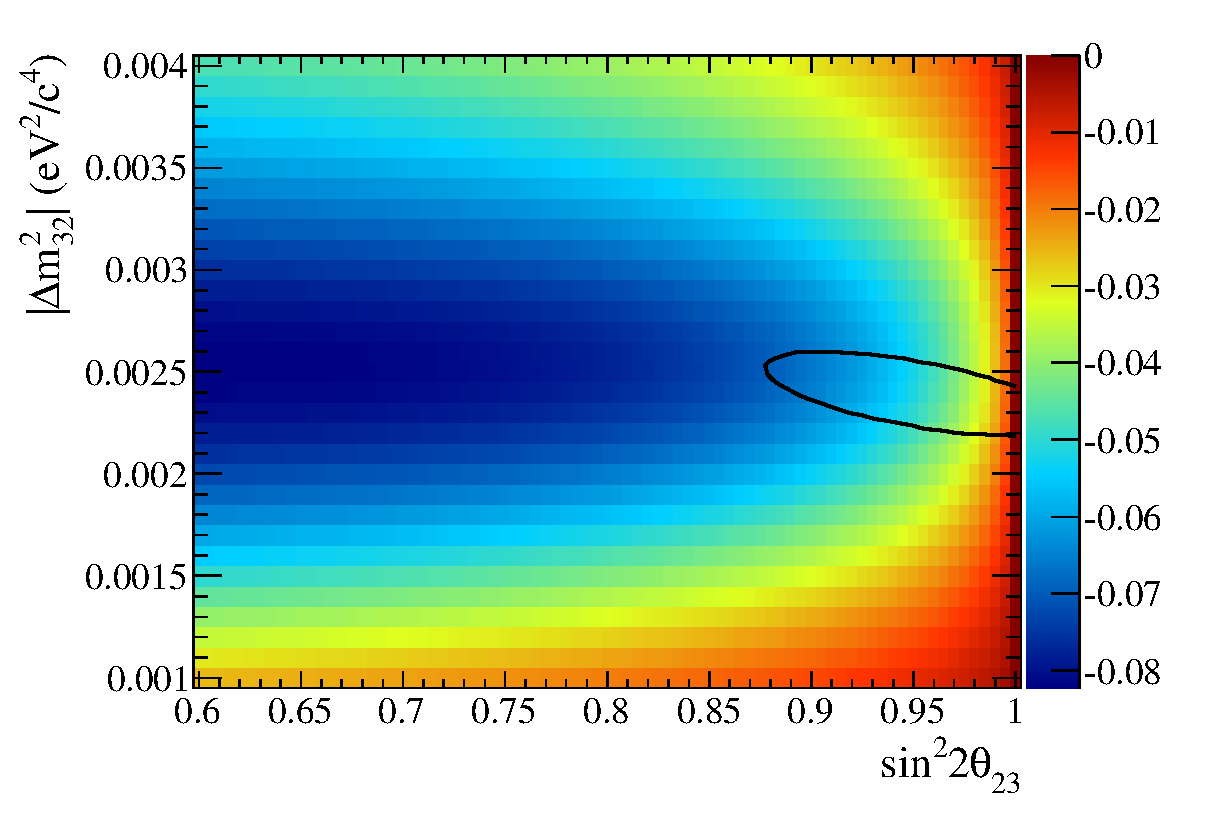
\includegraphics[width=18pc]{./images/spectrum_nominal/nsk_diff_octant}
\caption {
  Fractional difference in the predicted number of 1-ring $\mu$-like events between assuming that $\theta_{23}$ is in the first octant
  and assuming it is in the second octant.
  The fractional difference is shown as function of $\sin^{2}2\theta_{23}$ and $|\Delta m^{2}_{32}|$,
  for an exposure of 3.010$\times$10$^{20}$ POT.
  The number of events was calculated using the BANFF-tuned MC templates.
  The 2012 PDG values are used for $\sin^{2}2\theta_{13}$, $\sin^{2}2\theta_{12}$ and $\Delta m^{2}_{21}$, and $\delta_{CP}$=0.
  Results shown for the normal hierarchy.
  The 2012 MINOS 90\% confidence region is superimposed for reference.
}
\label{fig:nsk_vs_osc_params_tuned_mc_effect_of_octant}
\end{minipage}
\end{figure*}

%...........
%
% Effect of non-23 sector params 
% Effect of mass hierarchy
%
\begin{figure*}[htb]
\begin{minipage}[t]{0.48\linewidth}
\center
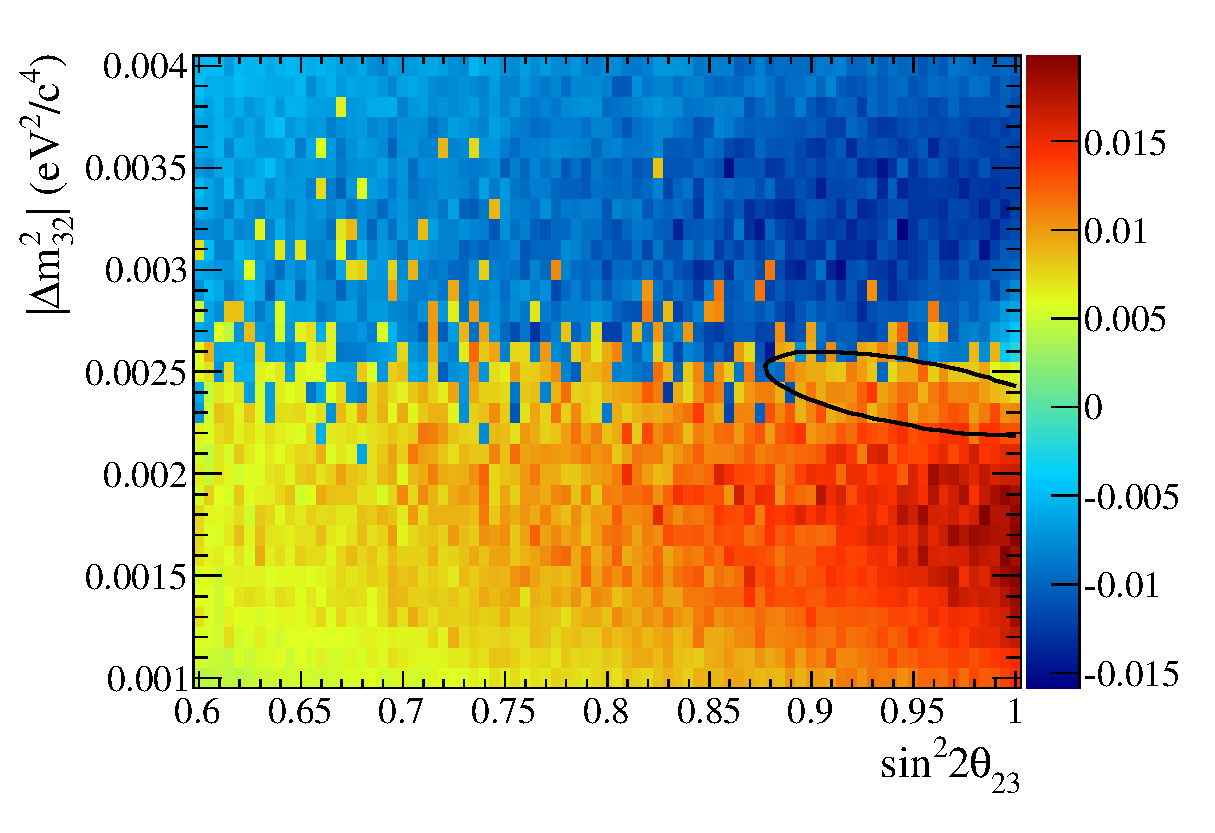
\includegraphics[width=18pc]{./images/spectrum_nominal/nsk_diff_non23throw}
\caption {
  Maximum value of the fractional difference in the predicted number of 1-ring $\mu$-like events
  between varying each of $\sin^{2}2\theta_{13}$, $\sin^{2}2\theta_{12}$, $\Delta m^{2}_{21}$ and $\delta_{CP}$ 
  within their allowed ranges and their nominal values (these are the 2012 PDG values for $\sin^{2}2\theta_{13}$, 
  $\sin^{2}2\theta_{12}$ and $\Delta m^{2}_{21}$, and $\delta_{CP}$=0).
  The fractional difference is shown as function of $\sin^{2}2\theta_{23}$ and $|\Delta m^{2}_{32}|$,
  for an exposure of 3.010$\times$10$^{20}$ POT.
  The number of events was calculated using the BANFF-tuned MC templates.
  The normal hierarchy was assumed.
  The 2012 MINOS 90\% confidence region is superimposed for reference.
}
\label{fig:nsk_vs_osc_params_tuned_mc_effect_of_non23}
\end{minipage}
\hspace{0.06\linewidth}
\begin{minipage}[t]{0.48\linewidth}
\center
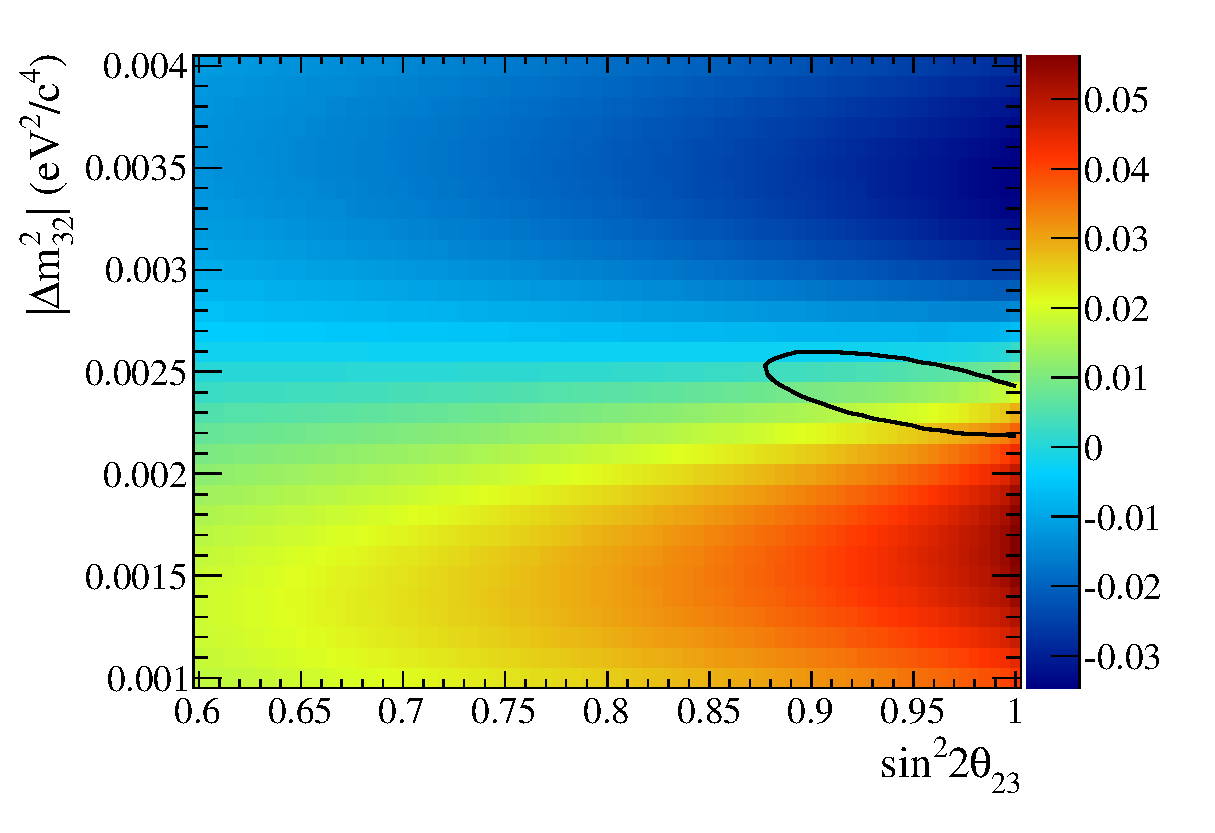
\includegraphics[width=18pc]{./images/spectrum_nominal/nsk_diff_inv}
\caption {
  Fractional difference in the predicted number of 1-ring $\mu$-like events between assuming the normal hierarchy 
  and assuming the inverted hierarchy.
  The fractional difference is shown as function of $\sin^{2}2\theta_{23}$ and $|\Delta m^{2}_{32}|$,
  for an exposure of 3.010$\times$10$^{20}$ POT.
  The number of events was calculated using the BANFF-tuned MC templates.
  The 2012 PDG values are used for $\sin^{2}2\theta_{13}$, $\sin^{2}2\theta_{12}$ and $\Delta m^{2}_{21}$, and $\delta_{CP}$=0. 
  The 2012 MINOS 90\% confidence region is superimposed for reference.
}
\label{fig:nsk_vs_osc_params_tuned_mc_effect_of_hierarchy}
\end{minipage}
\end{figure*}

\clearpage

\section {Systematic effects in the prediction of the single $\mu$-like ring event reconstructed energy spectrum}
\label{sec:systematics}

%....................................................................................................................
%....................................................................................................................

\subsection {Input systematic parameters}
\label{sec:systematics:inputs}

This analysis considers 48 systematic parameters which can be grouped into 4 categories:
\begin{enumerate}
\item SuperK detector parameters (Sec. \ref{sec:systematics:inputs:superk_det})
\item Correlated flux and cross-section parameters tuned by the BANFF group to ND280 data (Sec. \ref{sec:systematics:inputs:banff})
\item Uncorrelated cross-section parameters (Sec. \ref{sec:systematics:inputs:uncor_xsec})
\item Intranuclear and secondary interactions (Sec. \ref{sec:systematics:inputs:fsi}).
\end{enumerate}
A summary of all systematic parameters considered in this analysis is given in Tab.\ \ \ref{tab:input_uncertainties}.
These systematic parameters are applied to the MC templates as shown in Tab.\ \ \ref{tab:apply_syst_to_templates}.

%
% Summary table with systematic parameters
%

{
\begin{table*}[htb]
\thisfloatpagestyle{empty}
\small
\center
\renewcommand{\arraystretch}{1.75} % enlarge line spacing
\begin{tabular}{p{0.12\textwidth}p{0.65\textwidth}p{0.16\textwidth}}
%
% SuperK
%
\hline
\multicolumn {2}{l} { {\bf SuperK detector systematics} } \\
\hline
\parbox{0.12\textwidth}
{
   $f_{E; r}^{SK}$  
}&
\parbox{0.65\textwidth}
{
    \vspace{0.2cm}
    Reconstructed energy scale \\
}&
\parbox{0.16\textwidth}
{
  2.3\%
}\\
\parbox{0.12\textwidth}
{
   $f_{CCQERCi; r}^{SK}$
}&
\parbox{0.65\textwidth}
{
    \vspace{0.2cm}
    $\nu_\mu$, $\bar{\nu}_{\mu}$ CCQE ring-counting efficiency. 
    Three correlated systematic parameters are included (i=0,1,2) corresponding to different reconstructed energy ranges.
    See Sec.\ref{sec:systematics:inputs:superk_det}.\\
}&
\parbox{0.16\textwidth}
{
    1.7\% ($<$ 0.4 GeV) \\ 
    3.5\% (0.4-1.1 GeV) \\
    9.3\% ($>$ 1.1 GeV) 
}\\
\parbox{0.12\textwidth}
{
   $f_{CCQEoth; r}^{SK}$
}&
\parbox{0.65\textwidth}
{
    \vspace{0.2cm}
    $\nu_\mu$, $\bar{\nu}_{\mu}$ CCQE other (all but ring-counting) efficiency. 
    Includes fiducial volume, reduction chain, OD cut, PID cut, momentum cut and decay electron cut efficiencies. \\
}&
\parbox{0.16\textwidth}
{
  1.8\%
}\\
\parbox{0.12\textwidth}
{
   $f_{CCnonQE; r}^{SK}$
}&
\parbox{0.65\textwidth}
{
    \vspace{0.2cm}
    $\nu_\mu$, $\bar{\nu}_{\mu}$ CCnQE efficiency \\
}&
\parbox{0.16\textwidth}
{
  20\%
}\\
\parbox{0.12\textwidth}
{
   $f_{NC; r}^{SK}$
}&
\parbox{0.65\textwidth}
{
    \vspace{0.2cm}
    NC efficiency \\
}&
\parbox{0.16\textwidth}
{
  111\%
}\\
\parbox{0.12\textwidth}
{
   $f_{\nu_e; r}^{SK}$
}&
\parbox{0.65\textwidth}
{
    \vspace{0.2cm}
    $\nu_e$, $\bar{\nu}_{e}$ efficiency \\
}&
\parbox{0.16\textwidth}
{
  100\%
}\\
%
% BANFF systematics
%
\multicolumn {2}{l} { {\bf Correlated flux and cross-section (BANFF) systematics} } \\
\hline
\parbox{0.12\textwidth}
{ 
   $f_{i; t, r}^{banff}$  
}&
\parbox{0.65\textwidth}
{
    \vspace{0.2cm}
    Flux and cross-section parameters tuned by BANFF group on ND280 data.
    Twenty-three correlated parameters are included (i=0,...,22). 
    See Sec.\ \ref{sec:systematics:inputs:banff}.\\
}&
\parbox{0.16\textwidth}
{
  
}\\
\hline
%
% Neutrino Generator
%
\multicolumn {2}{l} { {\bf Uncorrelated cross-section systematics} } \\
\hline
\parbox{0.12\textwidth}
{ 
    \vspace{0.2cm}
    $f_{pF; t, r}$ 
}&
\parbox{0.65\textwidth}
{
    \vspace{0.2cm}
    Fermi momentum (CCQE only)\\ 
    %Applied to CCQE modes 
   
}&
\parbox{0.16\textwidth}
{
  225$\pm$30 MeV
}\\
\parbox{0.12\textwidth}
{ 
    \vspace{0.2cm}
    $f_{bindE; t, r}$ 
}&
\parbox{0.65\textwidth}
{
    \vspace{0.2cm}
    Binding energy for $^{16}O$ (CCQE only)\\
    %Applied to CCQE modes 
}&
\parbox{0.16\textwidth}
{
  27$\pm$9 MeV
}\\
\parbox{0.12\textwidth}
{ 
    \vspace{0.2cm}
    $f_{SF; t, r}$ 
}&
\parbox{0.65\textwidth}
{
    \vspace{0.2cm}
    Nuclear environment modeling; switch from Fermi Gas (RFG) to Spectral Function (SF) model (CCQE only).\\
}&
\parbox{0.16\textwidth}
{
  0 (RFG) - 1 (SF)
}\\
\parbox{0.12\textwidth}
{ 
    \vspace{0.2cm}
    $f_{\pi-less\Delta; t, r}$ 
}&
\parbox{0.65\textwidth}
{
    \vspace{0.2cm}
    Fraction of $\pi$-less $\Delta$ decays in resonance neutrino-production events\\
}&
\parbox{0.16\textwidth}
{
  20\%
}\\
\parbox{0.12\textwidth}
{ 
    \vspace{0.2cm}
    $f_{CCothShape; t, r}$ 
}&
\parbox{0.65\textwidth}
{
    \vspace{0.2cm}
    Parameterizes the uncertainty in CC multipion, CC DIS and CC resonant $\eta$, K and photon production. \\
}&
\parbox{0.16\textwidth}
{
  40\%
}\\
\parbox{0.12\textwidth}
{ 
    \vspace{0.2cm}
    $f_{Wshape; t, r}$ 
}&
\parbox{0.65\textwidth}
{
    \vspace{0.2cm}
    Modifies the shape of the initial pion momentum distribution (before final-state interactions) in resonance interactions. \\
}&
\parbox{0.16\textwidth}
{
  87.8$\pm$45.3
}\\
\parbox{0.12\textwidth}
{ 
    \vspace{0.2cm}
    $f_{CCcoh; t}$ 
}&
\parbox{0.65\textwidth}
{
    \vspace{0.2cm}
    CC coherent cross-section\\
    %Applied to the corresponding modes 
}&
\parbox{0.16\textwidth}
{
  100\%
   
}\\
\parbox{0.12\textwidth}
{ 
    \vspace{0.2cm}
    $f_{NC1\pi^\pm; t}$ 
}&
\parbox{0.65\textwidth}
{
    \vspace{0.2cm}
    NC1$\pi^\pm$ cross-section\\
    %Applied to the corresponding modes 
   
}&
\parbox{0.16\textwidth}
{
  30\%
}\\
\parbox{0.12\textwidth}
{ 
    \vspace{0.2cm}
    $f_{NCoth; t}$ 
}&
\parbox{0.65\textwidth}
{
    \vspace{0.2cm}
    NC other (all but single $\pi^\pm$) cross-section\\
    %Applied to the corresponding modes 
   
}&
\parbox{0.16\textwidth}
{
  30\%
}\\
\parbox{0.12\textwidth}
{ 
    \vspace{0.2cm}
    $f_{CC\nu_e; t}$ 
}&
\parbox{0.65\textwidth}
{
    \vspace{0.2cm}
    $\nu_e$ / $\nu_\mu$ CC cross-section ratio\\
    %Applied to the CC $\nu_e$ modes only 
   
}&
\parbox{0.16\textwidth}
{
  3\%
}\\
\parbox{0.12\textwidth}
{ 
    \vspace{0.2cm}
    $f_{CC\bar{\nu}; t}$ 
}&
\parbox{0.65\textwidth}
{
    \vspace{0.2cm}
    $\bar{\nu}$ / $\nu$ CC cross-section ratio\\
    %Applied to the CC $\bar{\nu}$ modes only 
   
}&
\parbox{0.16\textwidth}
{
  40\%
}\\
%
% FSI & SI
%
\multicolumn {2}{l} { {\bf FSI+SI systematics} } \\
\hline
\parbox{0.12\textwidth}
{ 
    \vspace{0.2cm}
    $f _{i; r}^{FSI}$ 
}&
\parbox{0.65\textwidth}
{
    \vspace{0.2cm}
    FSI (final state interaction / intranuclear hadron transport) and 
    SI (secondary interaction / detector hadron transport) systematic parameters. 
    Six correlated parameters are included (i=0,...,5) corresponding to different modes and reconstructed energy bins. 
    See Sec. \ref{sec:systematics:inputs:fsi}.\\
}&
\parbox{0.16\textwidth}
{
  
}\\
\hline
\end{tabular}\\[2pt]
\caption{
  Summary table of systematic parameters included the VaLOR $\nu_{\mu}$-disappearance analysis.
  The nuisance parameter symbols used in this paper are shown in the first column.
  An index r in the nuisance parameter symbol denotes dependence on reconstructed energy while an index t denotes 
  dependence on true energy.
  An index i is used where multiple systematic parameters, typically correlated between themselves, are grouped together;
  in these cases we refer you to the main text for the exact parameter definition and for the input covariance matrix.
  Wherever practical, 
  the physics parameter affected by the systematic parameter is shown in the second column
  and the size of the uncertainty is shown in the third column.
}
\label{tab:input_uncertainties}
\end{table*}
}

% ........................................


{
\setlength{\tabcolsep}{3pt}
\renewcommand{\arraystretch}{1.8}
\begin{table}
\tiny
\centering
\begin{tabular}{| c || c | c | c | c | c | c || c | c | c | c | c | c || c | c | c | c | c | c || c | c | c | c | c | c || c | c | c | c |}
\hline
                       & \begin{sideways}   $\nu_{\mu}$ CCQE                   \end{sideways}  &   
                         \begin{sideways}   $\nu_{\mu}$ CC1$\pi$               \end{sideways}  &   
                         \begin{sideways}   $\nu_{\mu}$ CC coherent            \end{sideways}  &   
                         \begin{sideways}   $\nu_{\mu}$ CC other               \end{sideways}  &   
                         \begin{sideways}   $\nu_{\mu}$ NC1$\pi^{\pm}$         \end{sideways}  &  
                         \begin{sideways}   $\nu_{\mu}$ NC other               \end{sideways}  &   
                         \begin{sideways}   $\bar{\nu_{\mu}}$ CCQE             \end{sideways}  &  
                         \begin{sideways}   $\bar{\nu_{\mu}}$ CC1$\pi$         \end{sideways}  &  
                         \begin{sideways}   $\bar{\nu_{\mu}}$ CC coherent      \end{sideways}  &  
                         \begin{sideways}   $\bar{\nu_{\mu}}$ CC other         \end{sideways}  &  
                         \begin{sideways}   $\bar{\nu_{\mu}}$ NC1$\pi^{\pm}$   \end{sideways}  &   
                         \begin{sideways}   $\bar{\nu_{\mu}}$ NC other         \end{sideways}  &   
                         \begin{sideways}   $\nu_{e}$ CCQE                     \end{sideways}  &   
                         \begin{sideways}   $\nu_{e}$ CC1$\pi$                 \end{sideways}  &   
                         \begin{sideways}   $\nu_{e}$ CC coherent              \end{sideways}  &  
                         \begin{sideways}   $\nu_{e}$ CC other                 \end{sideways}  &   
                         \begin{sideways}   $\nu_{e}$ NC1$\pi^{\pm}$           \end{sideways}  &   
                         \begin{sideways}   $\nu_{e}$ NC other                 \end{sideways}  &  
                         \begin{sideways}   $\bar{\nu_{e}}$ CCQE               \end{sideways}  &   
                         \begin{sideways}   $\bar{\nu_{e}}$ CC1$\pi$           \end{sideways}  &   
                         \begin{sideways}   $\bar{\nu_{e}}$ CC coherent        \end{sideways}  &   
                         \begin{sideways}   $\bar{\nu_{e}}$ CC other           \end{sideways}  &  
                         \begin{sideways}   $\bar{\nu_{e}}$ NC1$\pi^{\pm}$     \end{sideways}  & 
                         \begin{sideways}   $\bar{\nu_{e}}$ NC other           \end{sideways}  &   
                         \begin{sideways}   Osc-$\nu_{e}$ CCQE                 \end{sideways}  &   
                         \begin{sideways}   Osc-$\nu_{e}$ CC1$\pi$             \end{sideways}  &   
                         \begin{sideways}   Osc-$\nu_{e}$ CC coherent          \end{sideways}  &   
                         \begin{sideways}   Osc-$\nu_{e}$ CC other             \end{sideways}  \\
\hline
 $f_{E; r}^{SK}$             & \ck & \ck & \ck & \ck & \ck & \ck & \ck & \ck & \ck & \ck & \ck & \ck & \ck & \ck & \ck & \ck & \ck & \ck & \ck & \ck & \ck & \ck & \ck & \ck & \ck & \ck & \ck & \ck  \\
\hline
 $f_{CCQERC0; r}^{SK}$       & \ck &     &     &     &     &     & \ck &     &     &     &     &     &     &     &     &     &     &     &     &     &     &     &     &     &     &     &     &      \\
\hline
 $f_{CCQERC1; r}^{SK}$       & \ck &     &     &     &     &     & \ck &     &     &     &     &     &     &     &     &     &     &     &     &     &     &     &     &     &     &     &     &      \\
\hline
 $f_{CCQERC2; r}^{SK}$       & \ck &     &     &     &     &     & \ck  &     &     &     &     &     &     &     &     &     &     &     &     &     &     &     &     &     &     &     &     &      \\
\hline
 $f_{CCQEoth; r}^{SK}$       & \ck &     &     &     &     &     & \ck  &     &     &     &     &     &     &     &     &     &     &     &     &     &     &     &     &     &     &     &     &      \\
\hline
 $f_{CCnQE; r}^{SK}$         &     & \ck & \ck & \ck &     &     &     & \ck & \ck & \ck &     &     &     &     &     &     &     &     &     &     &     &     &     &     &     &     &     &      \\
\hline
 $f_{NC; r}^{SK}$            &     &     &     &     & \ck & \ck &     &     &     &     & \ck & \ck &     &     &     &     & \ck & \ck &     &     &     &     & \ck & \ck &     &     &     &      \\
\hline
 $f_{\nu_e; r}^{SK}$         &     &     &     &     &     &     &     &     &     &     &     &     & \ck & \ck & \ck & \ck &     &     & \ck & \ck & \ck & \ck &     &     & \ck & \ck & \ck & \ck  \\
\hline
 $f_{0; t, r}^{banff}$       & \ck & \ck & \ck & \ck & \ck & \ck &     &     &     &     &     &     &     &     &     &     &     &     &     &     &     &     &     &     &     &     &     &      \\ 
\hline
 $f_{1; t, r}^{banff}$       & \ck & \ck & \ck & \ck & \ck & \ck &     &     &     &     &     &     &     &     &     &     &     &     &     &     &     &     &     &     &     &     &     &      \\
\hline
 $f_{2; t, r}^{banff}$       & \ck & \ck & \ck & \ck & \ck & \ck &     &     &     &     &     &     &     &     &     &     &     &     &     &     &     &     &     &     &     &     &     &      \\
\hline
 $f_{3; t, r}^{banff}$       & \ck & \ck & \ck & \ck & \ck & \ck &     &     &     &     &     &     &     &     &     &     &     &     &     &     &     &     &     &     &     &     &     &      \\
\hline
 $f_{5; t, r}^{banff}$       & \ck & \ck & \ck & \ck & \ck & \ck &     &     &     &     &     &     &     &     &     &     &     &     &     &     &     &     &     &     &     &     &     &      \\
\hline
 $f_{6; t, r}^{banff}$       & \ck & \ck & \ck & \ck & \ck & \ck &     &     &     &     &     &     &     &     &     &     &     &     &     &     &     &     &     &     &     &     &     &      \\
\hline
 $f_{7; t, r}^{banff}$       & \ck & \ck & \ck & \ck & \ck & \ck &     &     &     &     &     &     &     &     &     &     &     &     &     &     &     &     &     &     &     &     &     &      \\
\hline
 $f_{8; t, r}^{banff}$       & \ck & \ck & \ck & \ck & \ck & \ck &     &     &     &     &     &     &     &     &     &     &     &     &     &     &     &     &     &     &     &     &     &      \\
\hline
 $f_{9; t, r}^{banff}$       & \ck & \ck & \ck & \ck & \ck & \ck &     &     &     &     &     &     &     &     &     &     &     &     &     &     &     &     &     &     &     &     &     &      \\
\hline
 $f_{10; t, r}^{banff}$      & \ck & \ck & \ck & \ck & \ck & \ck &     &     &     &     &     &     &     &     &     &     &     &     &     &     &     &     &     &     &     &     &     &      \\
\hline
 $f_{11; t, r}^{banff}$      &     &     &     &     &     &     & \ck & \ck & \ck & \ck & \ck & \ck &     &     &     &     &     &     &     &     &     &     &     &     &     &     &     &      \\
\hline
 $f_{12; t, r}^{banff}$      &     &     &     &     &     &     & \ck & \ck & \ck & \ck & \ck & \ck &     &     &     &     &     &     &     &     &     &     &     &     &     &     &     &      \\
\hline
 $f_{13; t, r}^{banff}$      &     &     &     &     &     &     & \ck & \ck & \ck & \ck & \ck & \ck &     &     &     &     &     &     &     &     &     &     &     &     &     &     &     &      \\
\hline
 $f_{14; t, r}^{banff}$      &     &     &     &     &     &     & \ck & \ck & \ck & \ck & \ck & \ck &     &     &     &     &     &     &     &     &     &     &     &     &     &     &     &      \\
\hline
 $f_{15; t, r}^{banff}$      &     &     &     &     &     &     & \ck & \ck & \ck & \ck & \ck & \ck &     &     &     &     &     &     &     &     &     &     &     &     &     &     &     &      \\
\hline
 $f_{16; t, r}^{banff}$      & \ck &     &     &     &     &     & \ck &     &     &     &     &     & \ck &     &     &     &     &     & \ck &     &     &     &     &     & \ck &     &     &      \\
\hline
 $f_{17; t, r}^{banff}$      &     & \ck &     & \ck & \ck & \ck &     & \ck &     & \ck & \ck & \ck &     & \ck &     & \ck & \ck & \ck &     & \ck &     & \ck & \ck & \ck &     &\ck  &     & \ck  \\
\hline
 $f_{18; t, r}^{banff}$      & \ck &     &     &     &     &     & \ck &     &     &     &     &     & \ck &     &     &     &     &     & \ck &     &     &     &     &     & \ck &     &     &      \\
\hline
 $f_{19; t, r}^{banff}$      & \ck &     &     &     &     &     & \ck &     &     &     &     &     & \ck &     &     &     &     &     & \ck &     &     &     &     &     & \ck &     &     &      \\
\hline
 $f_{20; t, r}^{banff}$      & \ck &     &     &     &     &     & \ck &     &     &     &     &     & \ck &     &     &     &     &     & \ck &     &     &     &     &     & \ck &     &     &      \\
\hline
 $f_{21; t, r}^{banff}$      &     & \ck &     &     &     &     &     & \ck &     &     &     &     &     & \ck &     &     &     &     &     & \ck &     &     &     &     &     & \ck &     &      \\
\hline
 $f_{22; t, r}^{banff}$      &     & \ck &     &     &     &     &     & \ck &     &     &     &     &     & \ck &     &     &     &     &     & \ck &     &     &     &     &     & \ck &     &      \\
\hline
 $f_{pF; t, r}$              & \ck &     &     &     &     &     & \ck &     &     &     &     &     & \ck &     &     &     &     &     & \ck &     &     &     &     &     & \ck &     &     &      \\
\hline
 $f_{SF; t, r}$              & \ck &     &     &     &     &     & \ck &     &     &     &     &     & \ck &     &     &     &     &     & \ck &     &     &     &     &     & \ck &     &     &      \\
\hline
 $f_{\pi-less\Delta; t, r}$  &     &\ck  &     &     & \ck & \ck &     & \ck &     &     & \ck & \ck &     & \ck &     &     &\ck  &\ck  &     & \ck &     &     & \ck & \ck &     & \ck &     &      \\
\hline
 $f_{bindE; t, r}$           & \ck &     &     &     &     &     & \ck &     &     &     &     &     & \ck &     &     &     &     &     & \ck &     &     &     &     &     & \ck &     &     &      \\
\hline
 $f_{CCothShape; t, r}$      &     &     &     &\ck  &     &     &     &     &     & \ck &     &     &     &     &     & \ck &     &     &     &     &     & \ck &     &     &     &     &     & \ck  \\
\hline
 $f_{Wshape; t, r}$          &     &     &     &     & \ck & \ck &     &     &     &     &\ck  & \ck &     &     &     &     & \ck & \ck &     &     &     &     &\ck  & \ck &     &     &     &      \\
\hline
 $f_{CCcoh; t}$              &     &     & \ck &     &     &     &     &     & \ck &     &     &     &     &     & \ck &     &     &     &     &     & \ck &     &     &     &     &     & \ck &      \\
\hline
 $f_{NC1\pi^\pm; t}$         &     &     &     &     & \ck &     &     &     &     &     & \ck &     &     &     &     &     & \ck &     &     &     &     &     & \ck &     &     &     &     &      \\
\hline
 $f_{NCoth; t}$              &     &     &     &     &     & \ck &     &     &     &     &     & \ck &     &     &     &     &     & \ck &     &     &     &     &     &\ck  &     &     &     &      \\
\hline
 $f_{CC\nu_e; t}$            &     &     &     &     &     &     &     &     &     &     &     &     & \ck & \ck & \ck &\ck  &     &     &\ck  &\ck  & \ck & \ck &     &     & \ck & \ck & \ck & \ck  \\
\hline
 $f_{CC\bar{\nu}; t}$        &     &     &     &     &     &     & \ck & \ck & \ck & \ck &     &     &     &     &     &     &     &     & \ck & \ck & \ck & \ck &     &     &     &     &     &     \\
\hline
 $f _{0; r}^{FSI}$           & \ck &     &     &     &     &     & \ck &     &     &     &     &     &     &     &     &     &     &     &     &     &     &     &     &     &     &     &     &      \\
\hline
 $f _{1; r}^{FSI}$           & \ck &     &     &     &     &     & \ck &     &     &     &     &     &     &     &     &     &     &     &     &     &     &     &     &     &     &     &     &      \\
\hline
 $f _{2; r}^{FSI}$           & \ck &     &     &     &     &     & \ck &     &     &     &     &     &     &     &     &     &     &     &     &     &     &     &     &     &     &     &     &      \\
\hline
 $f _{3; r}^{FSI}$           &     & \ck & \ck & \ck &     &     &     & \ck & \ck & \ck &     &     &     &     &     &     &     &     &     &     &     &     &     &     &     &     &     &      \\
\hline
 $f _{4; r}^{FSI}$           &     &     &     &     &     &     &     &     &     &     &     &     & \ck & \ck & \ck & \ck &     &     & \ck & \ck & \ck & \ck &     &     & \ck & \ck & \ck & \ck  \\
\hline
 $f _{5; r}^{FSI}$           &     &     &     &     & \ck & \ck &     &     &     &     & \ck & \ck &     &     &     &     & \ck & \ck &     &     &     &     & \ck & \ck &     &     &     &      \\
\hline
\end{tabular}
\caption{
  A \ck symbol denotes that the given MC template is modified when the given systematic parameter is tweaked.
  The table lists all 48 systematic parameters considered in this analysis (first column) and 
  all 28 MC templates used for constructing the single $\mu$-like ring event reconstructed energy spectrum p.d.f (first row).
}
\label{tab:apply_syst_to_templates}
\end{table}
}

%\clearpage

%....................................................................................................................
\subsubsection {SuperK detector systematics}
\label{sec:systematics:inputs:superk_det}

The SuperK detector systematics are unchanged from the 2010 analyses \cite{SuperkErrors}. 
They can be broken down into two categories:

\begin{enumerate}
\item Reconstructed energy scale\\ 
  The effect of the uncertainty in the reconstructed energy scale is calculated 
  by scaling the bin edges of the MC templates and,
  assuming uniform distribution of events within the bins, 
  calculating the number of events gained from / lost to neighbouring bins.
  The systematic parameter $f_{E; r}^{SK}$ controls the energy scale
  and its uncertainty is estimated to be 2.3\% \cite{SuperkErrors}.
  The effect of the energy scale uncertainty is propagated to all MC templates as shown in Tab.\ \ref{tab:apply_syst_to_templates}.\\
\item Detector efficiencies\\ 
  Uncertainty in the efficiencies comes from the uncertainties in the fiducial volume and reduction chain, 
  and the OD, ring-counting, PID, momentum and decay-electron cuts.
  The efficiency errors used in this analysis \cite{SuperkErrors} are listed below.
  \begin{itemize}
  \item $\nu_\mu$, $\bar{\nu}_{\mu}$ CCQE:\\
    An energy-dependent ring-counting efficiency error and an 
    energy-independent ``other'' efficiency error (due to all sources of uncertainty other than ring-counting)
    are taken into account.
    For the ring-counting effciciency, we assume correlated errors in 3 $E_{reco}$ bins: 0 - 0.4 GeV, 0.4 - 1.1 GeV and $>$ 1.1 GeV.
    The following error matrix is used:\\
    \\
    $
     \left(
        {\begin{array}{ccc}
           (1.7\%)^2  &   0.59 * 1.7\% * 3.5\%  &  0.33 * 1.7\% * 9.3\% \\
                      &   (3.5\%)^2             &  0.61 * 3.5\% * 9.3\% \\
                      &                         &  (9.3\%)^2            \\
         \end{array} }
     \right)
    $\\
    \\
    For the ``other'' efficiency, we assume an energy-independent error of 1.8\%.
  \item $\nu_\mu$, $\bar{\nu}_{\mu}$ CCnonQE:\\
        A single 20\% energy-independent error is assumed.
        This error was calculated by combining the quoted energy-independent 
        ring-counting (19.9\%) and other (1.7\%) errors in quadrature.
  \item NC:\\
        A single 111\% energy-independent error is assumed.
        This error was calculated by combining the quoted energy-independent 
        ring-counting (48.2\%), PID (100\%) and other (1.7\%) errors in quadrature. 
  \item $\nu_{e}$, $\bar{\nu}_{e}$ CC:\\
        A single $\sim$100\% energy-independent error is assumed.
  \end{itemize}

   The $\nu_\mu$ and $\bar{\nu}_{\mu}$ CCQE ring-counting efficiency is controlled by the systematic parameters
   $f_{CCQERC0; r}^{SK}$ ($E_{reco} <$ 0.4 GeV),
   $f_{CCQERC1; r}^{SK}$ (0.4 GeV $\leq E_{reco} \leq$ 1.1 GeV) and
   $f_{CCQERC2; r}^{SK}$ ($E_{reco} >$ 1.1 GeV), 
   while the ``other'' efficiency is controlled by parameter $f_{CCQEoth; r}^{SK}$.
   The $\nu_\mu$ and $\bar{\nu}_{\mu}$ CCnonQE, the NC and the $\nu_{e}$, $\bar{\nu}_{e}$ CC efficiencies
   are controlled by the systematic parameters
   $f_{CCnQE; r}^{SK}$, $f_{NC; r}^{SK}$ and $f_{\nu_e; r}^{SK}$ respectively.
   These systematic parameters are applied to the MC templates as specified in Tab.\ \ref{tab:apply_syst_to_templates}.
  
\end{enumerate}

\clearpage

%....................................................................................................................
\subsubsection {Correlated flux and cross-section (BANFF) systematics}
\label{sec:systematics:inputs:banff}

The postfit uncertainties of all BANFF flux and cross-section parameters 
and their correlations are taken into account.
A list of the BANFF parameters is given in Tab.\ \ref{tab:banff_params}. 
The BANFF postfit covariance matrix is shown in Fig.\ \ref{fig:banff_postcov},
while both postfit and prefit 1$\sigma$ fractional errors for all parameters
are shown in Fig.\ \ref{fig:banff_postcov_diag_sqrt}. These fractional errors are 
computed from the square roots of the diagonal elements of the corresponding input covariance matrix.

Version 8 of the BANFF matrix is used.

{
\renewcommand{\arraystretch}{1.5}
\begin{table}
\centering
\begin{tabular}{| c | c | c |}
\hline
 Parameter               &  Definition                                                &  Best-fit value (tune v8) \\
\hline
 $f_{0; t, r}^{banff}$   &  $\nu_\mu$ flux normalisation, E = 0.0 - 0.4 GeV           & 0.995 \\
 $f_{1; t, r}^{banff}$   &  $\nu_\mu$ flux normalisation, E = 0.4 - 0.5 GeV           & 1.007 \\
 $f_{2; t, r}^{banff}$   &  $\nu_\mu$ flux normalisation, E = 0.5 - 0.6 GeV           & 1.002 \\
 $f_{3; t, r}^{banff}$   &  $\nu_\mu$ flux normalisation, E = 0.6 - 0.7 GeV           & 0.963 \\
 $f_{4; t, r}^{banff}$   &  $\nu_\mu$ flux normalisation, E = 0.7 - 1.0 GeV           & 0.901 \\
 $f_{5; t, r}^{banff}$   &  $\nu_\mu$ flux normalisation, E = 1.0 - 1.5 GeV           & 0.910 \\
 $f_{6; t, r}^{banff}$   &  $\nu_\mu$ flux normalisation, E = 1.5 - 2.5 GeV           & 0.936 \\
 $f_{7; t, r}^{banff}$   &  $\nu_\mu$ flux normalisation, E = 2.5 - 3.5 GeV           & 0.967 \\
 $f_{8; t, r}^{banff}$   &  $\nu_\mu$ flux normalisation, E = 3.5 - 5.0 GeV           & 0.988 \\
 $f_{9; t, r}^{banff}$  &  $\nu_\mu$ flux normalisation, E = 5.0 - 7.0 GeV            & 0.997 \\
 $f_{10; t, r}^{banff}$  &  $\nu_\mu$ flux normalisation, E = 7.0 - 30.0 GeV          & 1.004 \\
\hline
 $f_{11; t, r}^{banff}$  &  $\bar{\nu}_{\mu}$ flux normalisation, E = 0.0 - 0.7 GeV     & 0.980 \\
 $f_{12; t, r}^{banff}$  &  $\bar{\nu}_{\mu}$ flux normalisation, E = 0.7 - 1.0 GeV     & 0.958 \\
 $f_{13; t, r}^{banff}$  &  $\bar{\nu}_{\mu}$ flux normalisation, E = 1.0 - 1.5 GeV     & 0.947 \\
 $f_{14; t, r}^{banff}$  &  $\bar{\nu}_{\mu}$ flux normalisation, E = 1.5 - 2.5 GeV     & 0.953 \\
 $f_{15; t, r}^{banff}$  &  $\bar{\nu}_{\mu}$ flux normalisation, E = 2.5 -30.0 GeV     & 0.985 \\
\hline
 $f_{16; t, r}^{banff}$  &  CCQE axial mass normalisation, $x_{MAQE}$                             & 1.049 \\
 $f_{17; t, r}^{banff}$  &  Resonant axial mass normation, $x_{MARES}$                        & 1.011 \\
 $f_{18; t, r}^{banff}$  &  CCQE normalisation, E = 0.0 - 1.5 GeV                     & 0.951 \\
 $f_{19; t, r}^{banff}$  &  CCQE normalisation, E = 1.5 - 3.5 GeV                     & 0.708 \\
 $f_{20; t, r}^{banff}$  &  CCQE normalisation, E = 3.5 - 30.0 GeV                    & 1.347 \\
 $f_{21; t, r}^{banff}$  &  CC1$\pi$ normalisation, E = 0.0 - 2.5 GeV                 & 1.370 \\
 $f_{22; t, r}^{banff}$  &  CC1$\pi$ normalisation, E = 2.5 - 30.0 GeV                & 1.016 \\
\hline
\end{tabular}
\caption{
  BANFF parameters and best-fit values (v8 tune) \cite{BANFF}.
}
\label{tab:banff_params}
\end{table}
}

Only the $\nu_\mu$ and $\bar{\nu_\mu}$ flux parameters are included in the BANFF fit.
The $\nu_e$ and $\bar{\nu_e}$ flux parameters have a negligible effect as shown by the results of the systematic study\footnote{
  The study was performed with an older version of the BANFF matrix (v5)} 
in Tab.\ \ref{tab:banff_fluxparams}.

Only those cross-section parameters that are expected to have some cancellation between the ND280 and SuperK are included in the BANFF fit.
The other cross-section parameters included in this analysis are taken to be uncorrelated with the flux parameters
and to have no cancellation between the near and far detectors.
These uncorrelated cross-section parameters are described in Sec.\ \ref{sec:systematics:inputs:uncor_xsec}.

The BANFF parameters are applied to the MC templates as specified in Tab.\ \ref{tab:apply_syst_to_templates}.
All but two of the BANFF cross-section parameters are simple normalization factors.
The parameters $f_{16; t, r}^{banff}$ and $f_{17; t, r}^{banff}$\footnote{
  $f_{16; t, r}^{banff}$ and $f_{17; t, r}^{banff}$ are not the \emph{value} of $M_{A}$, but
  instead a multiplicative factor describing how $M_{A}$ moves away from
  nominal; $M_A$ $\rightarrow$ $x_{MA} M_A$.
} parameterize
the effect of the uncertainty of the axial masses used for modeling CC quasi-elastic 
($M_{A}^{QE}$) 
\footnote{
  An alternative way to treat the quasielastic axial mass was suggested \cite{1overMAQE2}; use 1/$(M_{A}^{QE})^2$ instead of $M_{A}^{QE}$. 
  This is because 1/$(M_{A}^{QE})^2$ has a more linear response than $M_{A}^{QE}$. Distributions of the predicted number of events in SuperK 
  are shown in \cite{Tom1overMaQE2} for 20000 toy experiments with all BANFF matrix parameters randomly thrown for each of these two
  definitions of $M_{A}^{QE}$. Both are Gaussian, suggesting that there is no 
  effect of the $M_{A}^{QE}$ response on the far detector phase space. The shift is thought to be due to the different parameter ranges used: 
  $M_{A}^{QE}$ = 1.21$\pm$0.45 while 1/$(M_{A}^{QE})^2$ = 0.683$\pm$0.320, which translates to $M_{A}^{QE}$ = $1.21^{+0.45}_{−0.21}$. 
  Therefore it was decided to use $M_{A}^{QE}$, to be consistent with the 2012 $\nu_e$ analyses.
} and 
resonance neutrino-production ($M_{A}^{RES}$) 
events respectively;
these have a more complicated, often non-linear, dependence on the true and reconstructed neutrino energy.
Event reweighting methods were used to obtain the fractional changes of the number of events, 
in bins of true and reconstructed neutrino energy, for a range of values (-3.0$\sigma$, -2.5$\sigma$, -2.0$\sigma$, ..., +3.0$\sigma$)
of the $f_{17; t, r}^{banff}$ and $f_{18; t, r}^{banff}$ parameters.
In our p.d.f. calculation, cross-section splines using a polynomial of order 3 are used to interpolate between these event weights 
to obtain the fractional change for any value of these systematic parameters in the (-3.0$\sigma$, +3.0$\sigma$) range.


\begin{table}[htb]
  \centering
  \begin{tabular}{ | l | c c | c c | }
    \hline
    &  \multicolumn {2}{c|} {sin$^2(2\theta_{23})$ = 1.0) }  &  \multicolumn {2}{c|} {sin$^2(2\theta_{23})$ = 0.9} \\
    Systematic & $\delta$ sin$^2(2\theta_{23})$ & $\delta$ $|\Delta m^2_{32}|$  & $\delta$ sin$^2(2\theta_{23})$ & $\delta$ $|\Delta m^2_{32}|$ \\
    \hline
    Statistical & 0.17 & 0.00014 & 0.05 & 0.00022 \\
    \hline
    $\bar{\nu}_{\mu}$ flux 0.0-0.4 GeV & $1 \cdot 10^{-6}$ & $4 \cdot 10^{-7}$ & $5 \cdot 10^{-5}$ & $4 \cdot 10^{-7}$ \\
    $\bar{\nu}_{\mu}$ flux 0.4-0.5 GeV & $1 \cdot 10^{-6}$ & $3 \cdot 10^{-7}$ & $4 \cdot 10^{-5}$ & $4 \cdot 10^{-7}$ \\
    $\bar{\nu}_{\mu}$ flux 0.5-0.6 GeV & $< 1 \cdot 10^{-6}$ & $2 \cdot 10^{-7}$ & $4 \cdot 10^{-5}$ & $2 \cdot 10^{-7}$ \\
    $\bar{\nu}_{\mu}$ flux 0.6-0.7 GeV & $< 1 \cdot 10^{-6}$ & $1 \cdot 10^{-7}$ & $5 \cdot 10^{-5}$ & $2 \cdot 10^{-7}$ \\
    $\bar{\nu}_{\mu}$ flux 0.7-1.0 GeV & $2 \cdot 10^{-6}$ & $4 \cdot 10^{-7}$ & $12 \cdot 10^{-5}$ & $6 \cdot 10^{-7}$ \\
    $\bar{\nu}_{\mu}$ flux 1.0-1.5 GeV & $2 \cdot 10^{-6}$ & $11 \cdot 10^{-7}$ & $12 \cdot 10^{-5}$ & $17 \cdot 10^{-7}$ \\
    $\bar{\nu}_{\mu}$ flux 1.5-2.5 GeV & $1 \cdot 10^{-6}$ & $9 \cdot 10^{-7}$ & $4 \cdot 10^{-5}$ & $15 \cdot 10^{-7}$ \\
    $\bar{\nu}_{\mu}$ flux 2.5-3.5 GeV & $< 1 \cdot 10^{-6}$ & $2 \cdot 10^{-7}$ & $4 \cdot 10^{-5}$ & $2 \cdot 10^{-7}$ \\
    $\bar{\nu}_{\mu}$ flux 3.5-5.0 GeV & $< 1 \cdot 10^{-6}$ & $2 \cdot 10^{-7}$ & $4 \cdot 10^{-5}$ & $2 \cdot 10^{-7}$ \\
    $\bar{\nu}_{\mu}$ flux 5.0-7.0 GeV & $< 1 \cdot 10^{-6}$ & $2 \cdot 10^{-7}$ & $4 \cdot 10^{-5}$ & $2 \cdot 10^{-7}$ \\
    $\bar{\nu}_{\mu}$ flux 7.0-30.0 GeV & $< 1 \cdot 10^{-6}$ & $2 \cdot 10^{-7}$ & $4 \cdot 10^{-5}$ & $2 \cdot 10^{-7}$ \\
    \hline
    $\nu_e$ flux 0.0-0.5 GeV & $< 1 \cdot 10^{-6}$ & $2 \cdot 10^{-7}$ & $4 \cdot 10^{-5}$ & $2 \cdot 10^{-7}$ \\
    $\nu_e$ flux 0.5-0.7 GeV & $< 1 \cdot 10^{-6}$ & $2 \cdot 10^{-7}$ & $4 \cdot 10^{-5}$ & $2 \cdot 10^{-7}$ \\
    $\nu_e$ flux 0.7-0.8 GeV & $< 1 \cdot 10^{-6}$ & $2 \cdot 10^{-7}$ & $4 \cdot 10^{-5}$ & $2 \cdot 10^{-7}$ \\
    $\nu_e$ flux 0.8-1.5 GeV & $< 1 \cdot 10^{-6}$ & $2 \cdot 10^{-7}$ & $4 \cdot 10^{-5}$ & $2 \cdot 10^{-7}$ \\
    $\nu_e$ flux 1.5-2.5 GeV & $< 1 \cdot 10^{-6}$ & $2 \cdot 10^{-7}$ & $4 \cdot 10^{-5}$ & $2 \cdot 10^{-7}$ \\
    $\nu_e$ flux 2.5-4.0 GeV & $< 1 \cdot 10^{-6}$ & $2 \cdot 10^{-7}$ & $4 \cdot 10^{-5}$ & $2 \cdot 10^{-7}$ \\
    $\nu_e$ flux 4.0-30.0 GeV & $< 1 \cdot 10^{-6}$ & $2 \cdot 10^{-7}$ & $4 \cdot 10^{-5}$ & $2 \cdot 10^{-7}$ \\
    \hline
    $\bar{\nu}_{e}$ flux 0.0-2.5 GeV & $< 1 \cdot 10^{-6}$ & $2 \cdot 10^{-7}$ & $4 \cdot 10^{-5}$ & $2 \cdot 10^{-7}$ \\
    $\bar{\nu}_{e}$ flux 2.5-30.0 GeV & $< 1 \cdot 10^{-6}$ & $2 \cdot 10^{-7}$ & $4 \cdot 10^{-5}$ & $2 \cdot 10^{-7}$ \\
    \hline
  \end{tabular}
  \caption{
    Maximum deviation from input values of oscillation parameters for a 2+0 fit and a single parameter $\pm$1 sigma deviation from nominal.
    This uses an old version of the BANFF matrix (v5) with a different parameter set.
    The $\nu_e$ and $\bar{\nu}_{e}$ flux parameters have negligible effect, and they were removed for BANFF v8.
    Similiarly, the first four and last four $\bar{\nu_\mu}$ flux parameters have negligible effect, and these were combined for BANFF v8.
    Made for oscillations with 
    $\sin^22\theta_{12} = $0.857; $\sin^22\theta_{13} = $0.098; $\delta_{CP} = $
    0; $\Delta m^2_{12} = $ 7.5e-05 $eV^{2}/c^{4}$; $|\Delta m^2_{32}| = $ 0.0024 $eV^{2}/c^{4}$
    and  for an exposure of 3.010$\times$10$^{20}$ POT.
  }
  \label{tab:banff_fluxparams}
\end{table}

%
% covariance matrix and errs
%
\begin{figure*}[htb]
\begin{minipage}[t]{0.48\linewidth}
\center
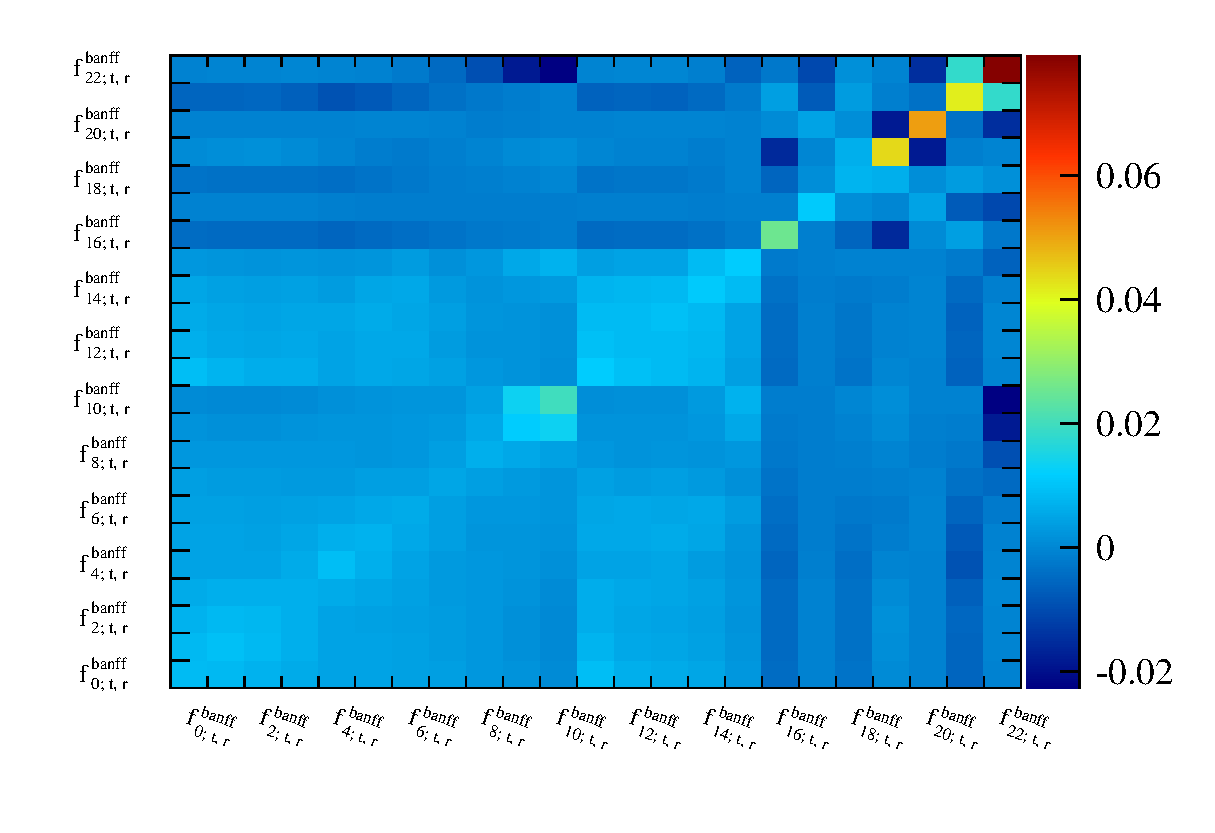
\includegraphics[width=20pc]{./images/spectrum_tweaked/banff}
\caption {
   The input BANFF postfit covariance matrix.
   The meaning of each parameter is given in the text.
}
\label{fig:banff_postcov}
\end{minipage}
\hspace{0.06\linewidth}
\begin{minipage}[t]{0.48\linewidth}
\center
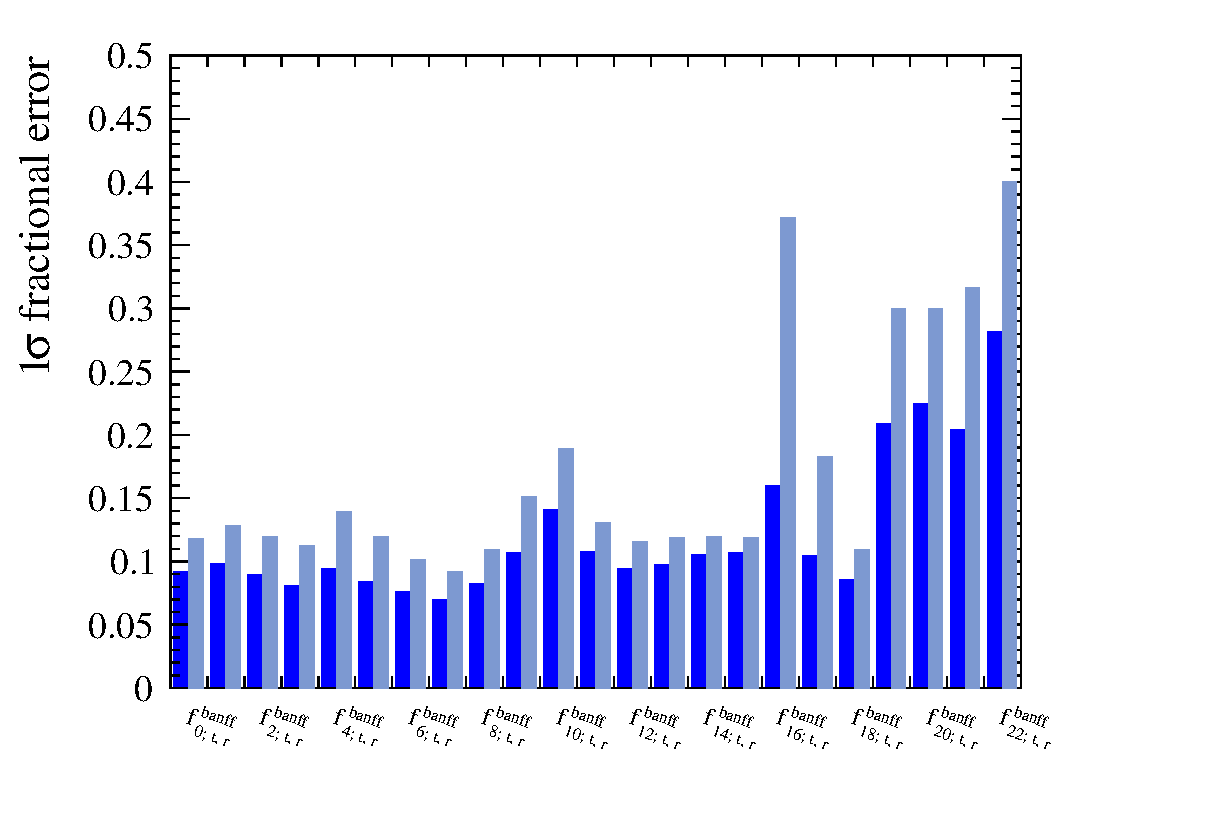
\includegraphics[width=20pc]{./images/spectrum_tweaked/banff_diag_sqrt}
\caption {
   Postfit (dark blue) and prefit (light blue) 1$\sigma$ fractional errors for BANFF parameters
   (computed from the square root of the diagonal elements of the corresponding input covariance matrix).
   The meaning of each parameter is given in the text.
}
\label{fig:banff_postcov_diag_sqrt}
\end{minipage}
\end{figure*}

%....................................................................................................................
\subsubsection {Uncorrelated cross-section systematics}
\label{sec:systematics:inputs:uncor_xsec}

In addition to the BANFF cross-section systematics,
another 11 cross-section systematics are taken into account; these additional systematics are considered to be uncorrelated 
between themselves and to have no cancellation between the near and far detectors \cite{NIWGErr} \cite{MoreNIWGErr113}.

Three of these additional systematics relate to the initial-state nuclear environment modeling for CCQE.
Neutrino Monte Carlo generators typically use Relativistic Fermi Gas (RFG) models,
with or without extensions to take nucleon-nucleon correlation into account, 
and with some, often simplistic, prescription for the treatment of off-shell kinematics.
The RFG model implementation depends on two parameters, the Fermi momentum level (225 MeV for $^{16}O$)
and the nucleon binding energy (27 MeV for $^{16}O$), which are extacted from quasi-elastic electron scattering data.
The systematic parameter $f_{pF; t, r}$ takes into account the effect of a 30 MeV 1$\sigma$ uncertainty in the Fermi momentum level
for $^{16}O$, while parameter $f_{bindE; t, r}$ takes into account the effect of a 9 MeV 1$\sigma$ uncertainty in the nucleon 
binding energy for for $^{16}O$.
The implementation details of the nuclear model can have a significant effect and, therefore,
the effect of switching between two such models was also included as a systematic uncertainty.
This analysis considers the effect of switching between the RFG model and a better-motivated 
Spectral Function (SF) model. The latter does not assume a fixed binding energy and includes the 
correlations between nucleon momentum and binding energy. The systematic parameter $f_{SF; t, r}$ 
includes the effect of switching between the two models.

Simple, energy-independent, generator-level uncertainties are considered for the CC coherent, NC, $\nu_e$ CC
and $\bar{\nu}$ CC cross sections, as the effect of these processes in the single $\mu$-like ring sample is small.
This analysis uses a 100\% uncertainty for the CC coherent cross-section, 
a 30\% uncertainty for both the NC1$\pi^\pm$ and NC ``other'' (all but single $\pi^\pm$) cross section,
a 3\% uncertainty on the $\nu_e$ / $\nu_\mu$ CC cross-section ratio and 
a 40\% uncertainty on the $\bar{\nu}$ / $\nu$ CC cross-section ratio.
The effect of the variation of the above cross sections is included in the analysis
through the systematic parameters $f_{CCcoh; t}$, $f_{NC1\pi^\pm; t}$, $f_{NCoth; t}$,
$f_{CC\nu_e; t}$ and $f_{CC\bar{\nu}; t}$ respectvely.

The treatment of $\Delta$ resonances in the nuclear environment has been controversial in the neutrino
Monte Carlo generator community. Certain models include a ~20\%-level of $\pi$-less $\Delta$ decays in order
to include the effect of $\Delta+N \rightarrow N+N$ scattering, in which the $\Delta$ interacts before it can decay. 
In contrast, other models include no $\pi$-less 
$\Delta$ decays on the basis that this would amount to double counting since, whatever the size of the effect, 
it is already included in hadron-nucleus scattering data to which the intranuclear cascade Monte Carlos are tuned.
This analysis uses NEUT, in which 20\% of $\Delta$s have a $\pi$-less decay by default, and takes the uncertainty in this 
branching fraction to be 100\%. 
The systematic parameter $f_{\pi-less\Delta; t, r}$ includes the effect of varying the fraction of $\pi$-less $\Delta$ 
decays to the corresponding MC templates.

The $f_{CCothShape;t,r}$ systematic parameterizes the uncertainty in CC multi-pion, CC deep inelastic scattering and CC $\eta$, 
K and photon production. From MINOS data, this is known to be $\approx$10\% at 4 GeV. Using this as a reference point, 
the uncertainty is estimated as 0.4/E$_{\nu}$, where E$_{\nu}$ is in GeV. It might appear that this error could diverge at 
low energy, but this does not happen since the threshold is $\approx$0.6 GeV and there are very 
few interactions below 1 GeV. 

The $f_{Wshape;t,r}$ parameter modifies the shape of the initial pion momentum distribution (before final-state interactions) 
by changing the distribution of the pion/nucleon invariant mass while keeping the total cross section constant. As the 
W shape parameter decreases, the pion momentum shifts to lower values, and this increases the probability of pion 
absorption in a final-state interaction. If such an absorption occurs, the event is migrated from CC1$\pi$ (its 
true initial state) and appears to be CCQE.

The effect of the $f_{CCcoh; t}$, $f_{NC1\pi^\pm; t}$, $f_{NCoth; t}$, $f_{CC\nu_e; t}$ and $f_{CC\bar{\nu}; t}$ 
systematic parameters is a simple normalisation change for the corresponding MC templates and thus easily implemented.
Systematic parameters $f_{pF; t, r}$, $f_{SF; t, r}$, $f_{bindE; t, r}$, $f_{\pi-less\Delta; t, r}$, $f_{CCothShape; t, r}$ 
and $f_{Wshape; t, r}$  have a complicated, often non-linear, dependance on true and reconstructed energy.
These are treated in a similar way to the BANFF parameters $f_{17; t, r}^{banff}$ and $f_{18; t, r}^{banff}$ (see Sec.\ 
\ref{sec:systematics:inputs:banff}).
Event reweighting methods were used to obtain the fractional changes of the number of events, 
in bins of true and reconstructed neutrino energy, for a range of values (-3.0$\sigma$, -2.5$\sigma$, -2.0$\sigma$, ..., +3.0$\sigma$)
of the systematic parameters. Again cross-section splines with polynomials of order 3 were used to interpolate between these event 
weights to obtain the fractional change for any
value of these systematic parameters in the (-3.0$\sigma$, +3.0$\sigma$) range.

Some of these systematics are special cases:
\begin{itemize}
\item 
  $f_{SF; t, r}$ is discrete; it can be either off (RFG) or on (SF). 
  Splines are generated with off as nominal, and on as +1.0 sigma.
  Linear interpolation is done only between the weights for 0 and 1.
\item 
  For $f_{Wshape; t, r}$ only $\pm$1.0 sigma errors are evaluated using event reweighting. 
  All other errors are extrapolated or interpolated from these $\pm$1.0 weights.
\item 
  For $f_{\\pi-less\\Delta; t, r}$ only $\pm$1.0 sigma errors are evaluated using event reweighting.
  Weights for tweaks more positive than +1$\sigma$ are extrapolated from the +1$\sigma$ weight. Weights more negative than 
  -1$\sigma$ are taken to be the same as the -1$\sigma$ weight; this is done since 20\% of deltas have a piless decay by 
  default in NEUT, and the error is 20\%. For this reason, it is unphysical to tweak $f_{\\pi-less\\Delta; t, r}$ to be 
  more negative than -1$\sigma$. 
\end{itemize}

The cross-section splines have 41 bins in reconstructed energy:
\begin{itemize}
\item 1 bin from 0-0.3 GeV
\item 14 50-MeV bins from 0.3-1.0 GeV
\item 20 100MeV bins from 1.0-3.0 GeV
\item 2 500-MeV bins from 3.0-4.0 GeV
\item 1 bin from 4.0-5.0 GeV
\item 1 bin from 5.0-7.0 GeV
\item 1 bin from 7.0-10.0 GeV
\item 1 bin from 10.0-30.0 GeV
\end{itemize}
For the $\nu_{\mu}$, $\bar{\nu}_{\mu}$ and oscillated $\nu_{e}$ samples, they have 11 bins in true energy:
\begin{itemize}
\item 1 bin from 0-0.4 GeV
\item 3 100-MeV bins from 0.4-0.7 GeV
\item 1 bin from 0.7-1.0 GeV
\item 1 bin from 1.0-1.5 GeV
\item 2 1-GeV bins from 1.5-3.5 GeV
\item 1 bin from 3.5-5.0 GeV
\item 1 bin from 5.0-7.0 GeV
\item 1 bin from 7.0-30.0 GeV  
\end{itemize}
For the $\nu_{e}$ sample, they have 7 bins in true energy:
\begin{itemize}
\item 1 bin from 0-0.05 GeV
\item 1 bin from 0.5-0.7 GeV
\item 1 bin from 0.7-0.8 GeV
\item 1 bin from 0.8-1.5 GeV
\item 1 bin from 1.5-2.5 GeV
\item 1 bin from 2.5-4.0 GeV
\item 1 bin from 4.0-30.0 GeV 
\end{itemize}
Finally, for the $\bar{\nu}_{e}$ sample, they have 2 bins in true energy:
\begin{itemize}
\item 1 bin from 0-2.5 GeV
\item 1 bin from 2.5-30.0 GeV
\end{itemize}

An example of a cross-section spline is shown in Fig.\ \ref{fig:example_spline}. 

\begin{figure}[htb]
\center
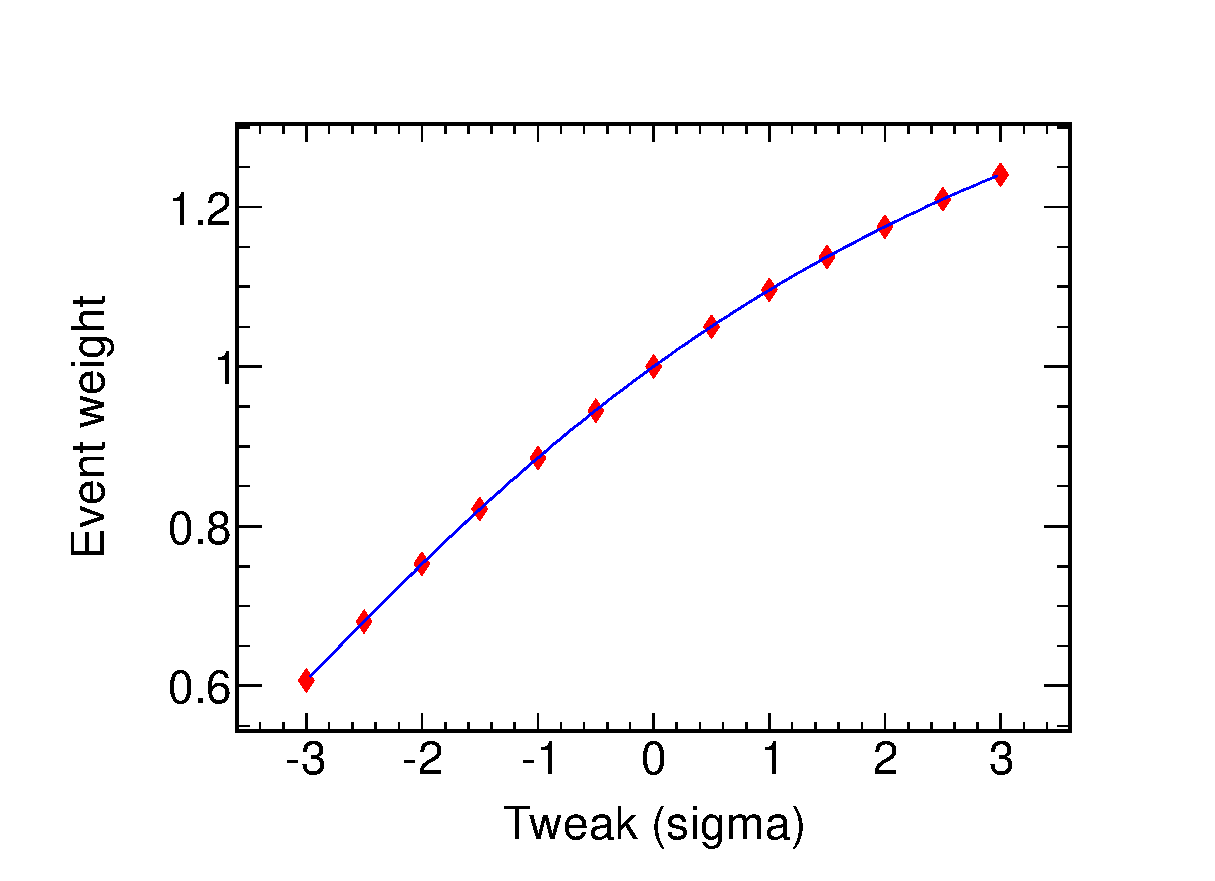
\includegraphics[width=25pc]{./images/spectrum_tweaked/ExampleSpline}
\caption {
Example of a cross-section spline; this shows the event weights obtained by tweaking $M_{A}^{QE}$
for $\nu_{\mu}$-CCQE events in the bin with reconstructed energy 0.75-0.8 GeV and 
true energy 0.6-0.7 GeV.
}
\label{fig:example_spline}
\end{figure}


The 11 uncorrelated cross-section systematics considered in this analysis are summarised in Tab.\ \ref{tab:input_uncertainties}.
These cross-section systematics are applied to the MC templates as shown in Tab.\ \ref{tab:apply_syst_to_templates}.


%....................................................................................................................
\subsubsection {FSI+SI systematics}
\label{sec:systematics:inputs:fsi}

Intranuclear hadron transport, or final-state interactions (FSI),
have significant effects in the T2K energy range and
result in event topologies, for scattering on nuclear targets, which are drastically different
compared with those created in neutrino scattering on free nucleons.
Elastic and inelastic hadron rescattering, secondary pion production, single and double charge exchange
and absorption followed by multi-nucleon knockout are typically modelled in neutrino event generators using
intranuclear cascades.

Uncertainties due to FSI were estimated by simultaneously varying the NEUT parameters that scale the interaction probabilities for quasi-elastic 
scattering, absorption, charge exchange and pion production using the method described in Sec.\ 2 in \cite{NIWGErr}. The NIWG group produced 16 
parameter sets that span the 1$\sigma$ surface in the parameter space; this was done by varying the NEUT parameters when running the pion scattering 
simulations, and comparing the results with external pion-carbon scattering data. These 16 parameter sets are shown in Tab.\ 2 in \cite{NIWGErr}. 

Uncertainties due to secondary pion interactions (SI) were also evaluated. The NIWG group adapted the NEUT nuclear cascade model to simulate SI in the 
SuperK detector simulation (SKDETSIM) and to allow variations in the interaction probabilities. Details of this are given in \cite{SI}. The original 
11c SKMC files do not contain all the truth information required for reweighting SI, and a second production was made. The two productions contain 
independent steps (SKDETSIM was rerun on the NEUT files), and there are small differences in the numbers of events between the productions. The second 
production was used only to produce the FSI+SI covariance matrix, which is shown in Fig.\ \ref{fig:fsi_covmatrix}. 
The 1$\sigma$ fractional errors in the 6 FSI+SI parameters are shown in Fig.\ \ref{fig:fsi_covmatrix_diag_sqrt}; these are computed from the square 
roots of the diagonal elements of the input covariance matrix.

Since the same model is used for FSI and SI, it is possible to evaluate the uncertainties in both FSI and SI simultaneously. This was done by 
reweighting a single $\mu$-like ring selected SK MC with the 16 FSI parameter sets using T2KReweight. The reweighting method for FSI is described 
in Sec. 8 in \cite{NEUTnuclear}. Variations in the SI interaction probabilities were included for each FSI parameter set.  Subsequently a covariance 
matrix was calculated using equation 1 in \cite{NIWGErr}; the quantity p in that equation is the average event weight for a FSI parameter set, and 
the sum is over the parameter sets.

The covariance matrix was made with a 6-bin scheme, as shown in Tab.\ \ref{tab:fsi_si_params}.
For $\nu_\mu$, $\bar{\nu}_{\mu}$ CCQE, the FSI+SI binning scheme
is identical to that used by SuperK for calculating the $\nu_\mu$, $\bar{\nu}_{\mu}$ CCQE ring-counting efficiency error matrix.

{
\renewcommand{\arraystretch}{1.5}
\begin{table}
\centering
\begin{tabular}{| c | c |}
\hline
 Parameter               &  Definition \\
\hline
 $f _{0; r}^{FSI}$       &  $\nu_\mu$ \& $\bar{\nu}_{\mu}$ CCQE, $E_{reco}<$ 0.4 GeV  \\
 $f _{1; r}^{FSI}$       &  $\nu_\mu$ \& $\bar{\nu}_{\mu}$ CCQE, 0.4 GeV $\leq E_{reco} \leq$ 1.1 GeV \\
 $f _{2; r}^{FSI}$       &  $\nu_\mu$ \& $\bar{\nu}_{\mu}$ CCQE, $E_{reco}>$ 1.1 GeV \\
 $f _{3; r}^{FSI}$       &  $\nu_\mu$ \& $\bar{\nu}_{\mu}$ CCnonQE \\
 $f _{4; r}^{FSI}$       &  $\nu_e$, $\bar{\nu}_{e}$ CC \\
 $f _{5; r}^{FSI}$       &  All NC \\
\hline
\end{tabular}
\caption{
  FSI+SI systematic parameters.
}
\label{tab:fsi_si_params}
\end{table}
}

%
% Input FSI param covariance & errs
%
\begin{figure*}[htb]
\begin{minipage}[t]{0.48\linewidth}
\center
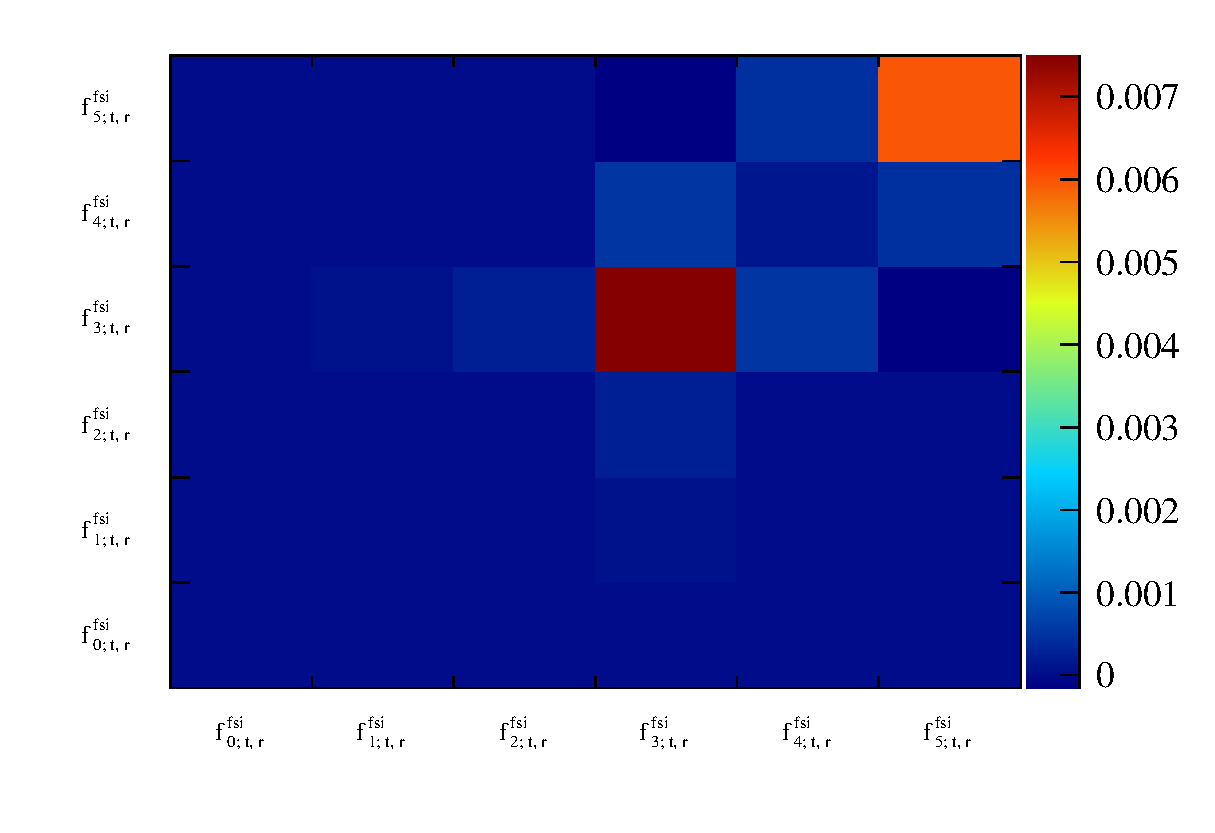
\includegraphics[width=20pc]{./images/spectrum_tweaked/fsi}
\caption {
  The input FSI+SI covariance matrix.
  The meaning of each parameter is given in Tab.\ \ref{tab:fsi_si_params}.
}
\label{fig:fsi_covmatrix}
\end{minipage}
\hspace{0.06\linewidth}
\begin{minipage}[t]{0.48\linewidth}
\center
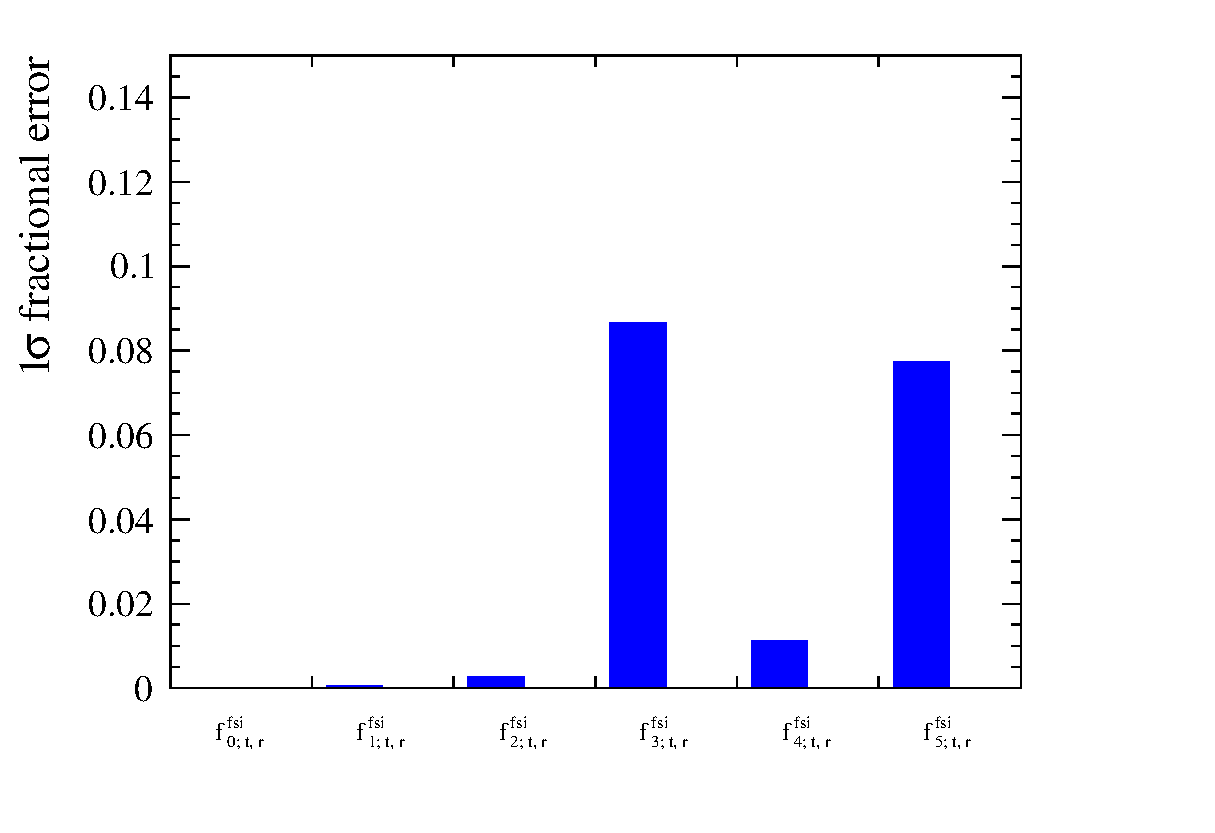
\includegraphics[width=20pc]{./images/spectrum_tweaked/fsi_diag_sqrt}
\caption {
   1$\sigma$ fractional error for FSI+SI parameters
   (computed from the square roots of the diagonal elements of the input covariance matrix).
  The meaning of each parameter is given in Tab.\ \ref{tab:fsi_si_params}.
}
\label{fig:fsi_covmatrix_diag_sqrt}
\end{minipage}
\end{figure*}

%....................................................................................................................
%....................................................................................................................

\subsection {Evaluation of systematic effects on the single $\mu$-like ring reconstructed energy spectrum}
\label{sec:systematics:evaluation}

In this section, we present the effects of the systematics described in Secs.\ \ref{sec:systematics:inputs:banff}, 
\ref{sec:systematics:inputs:uncor_xsec} and \ref{sec:systematics:inputs:fsi} on the expected 
number of single $\mu$-like ring events and the reconstructed energy spectrum in SuperK.
These effects are shown both for no oscillations and for oscillations with
$\sin^{2}2\theta_{23}$ = 1.0 and $|\Delta m^{2}_{32}|$ = 2.4$\times10^{-3}$ $eV^{2}/c^{4}$.
For the oscillation cases, the 2012 PDG values are used for $\sin^{2}2\theta_{13}$, $\sin^{2}2\theta_{12}$ and $\Delta m^{2}_{21}$,
and $\delta_{CP}$=0. The normal mass hierarchy is assumed.
All results are generated for an integrated exposure of 3.010$\times$10$^{20}$ POT and
the BANFF-tuned MC templates are used.

The effects of systematic uncertainties on the expected number of events, both for no oscillations and for oscillations 
with the typical parameter values given above, is summarised in Tab.\ \ref{tab:nsk_systematic_table_summary}.
In this table, systematic parameters are grouped into a few categories and all parameter correlations are taken into account.
Entries for both the BANFF prefit and postfit errors are provided.
The effects of each parameter individually are presented in Tab.\ \ref{tab:nsk_systematic_table} in which the correlations 
between parameters are necessarily ignored.

The effects of the combined systematic uncertainties on the reconstructed energy spectrum of single $\mu$-like ring events
is shown in Fig.\ \ref{fig:1Rmu_error_envelope_total}, for the typical oscillation scenario used.
This plot shows the total error envelope for the 1 $\mu$-like ring event reconstructed energy spectrum; this is calculated 
as the $\pm$1$\sigma$ spread of bin contents from 100k toy MC experiments generated with randomized systematic parameters.
In Fig.\ \ref{fig:1Rmu_error_envelope_total}, all systematic parameters were considered and their correlations were taken 
into account.

Error envelopes from the effects of certain groups of systematic parameters are shown in  
Figs.\ \ref{fig:1Rmu_error_envelope_superk_det} (SuperK detector systematics only), 
\ref{fig:1Rmu_error_envelope_banff} (BANFF systematics only), 
\ref{fig:1Rmu_error_envelope_uncor_xsec} (uncorrelated cross-section systematics only), and 
\ref{fig:1Rmu_error_envelope_fsi} (FSI+SI systematics only).

Detailed studies showing the effects of individual systematics on the expected number of
single $\mu$-like ring events are shown in Appendix \ref{appendix:nsk_systematics},
while their effects on the reconstructed energy spectrum of the single $\mu$-like ring sample
are shown in Appendix \ref{appendix:spectrum_systematics}.

%..................

\begin{table}
\centering
\begin{tabular}{| c | c | c |}
\hline
  {\bf Source of uncertainty}  &  {\bf ${\delta}N_{SK}$/$N_{SK}$}  & {\bf ${\delta}N_{SK}$/$N_{SK}$} \\
                               &  (no oscillation)                 & (oscillations with typical parameter values) \\
\hline
SuperK detector       &  5.57\%   & 10.08\%  \\
BANFF (prefit)        & 24.14\%   & 21.84\%  \\
BANFF (postfit)       &  4.38\%   &  4.15\%  \\
Uncorrelated XSec     &  3.64\%   &  6.26\%  \\
FSI+SI                &  1.87\%   &  3.48\%  \\
\hline
Total (BANFF prefit)  & 25.11\%   & 25.10\%  \\
Total (BANFF postfit) &  8.18\%   & 13.04\%  \\
\hline
\end{tabular}
\caption{
  Effect of 1$\sigma$ systematic parameter variation on
  the number of 1-ring $\mu$-like events,
  computed
  for no oscillations and
  for oscillations with 
  $\sin^{2}2\theta_{23}$=1.0 and $|\Delta m^{2}_{32}|$=2.4$\times10^{-3}$ $eV^{2}/c^{4}$.
  For the oscillation scenario, the 2012 PDG values are used for $\sin^{2}2\theta_{13}$, $\sin^{2}2\theta_{12}$ and $\Delta m^{2}_{21}$,
  and $\delta_{CP}$=0. The normal mass hierarchy is assumed.
  The numbers shown were calculated for an exposure of 3.010$\times$10$^{20}$ POT and BANFF-tuned MC templates were used.
}
\label{tab:nsk_systematic_table_summary}
\end{table}

%..................

\begin{table}
\centering
\begin{tabular}{| c || c | c || c | c |}
\hline
  Source of uncertainty        &  \multicolumn {2}{c||}{${\delta}N_{SK}$/$N_{SK}$} & \multicolumn {2}{c||}{${\delta}N_{SK}$/$N_{SK}$} \\
                               &  \multicolumn {2}{c||}{(no oscillation)}          & \multicolumn {2}{c||}{(oscillations with typical params)} \\
                               & BANFF prefit & BANFF postfit & BANFF prefit & BANFF postfit \\
\hline
$f_{E; r}^{SK}$               & 0.00 & 0.00 & 0.00 & 0.00 \\
$f_{CCQEoth; r}^{SK}$         & 1.41 & 1.41 & 0.97 & 0.97 \\
$f_{CCQERC0; r}^{SK}$         & 0.06 & 0.06 & 0.11 & 0.11 \\
$f_{CCQERC1; r}^{SK}$         & 2.22 & 2.22 & 0.83 & 0.83 \\
$f_{CCQERC2; r}^{SK}$         & 0.96 & 0.96 & 2.30 & 2.30 \\
$f_{CCnQE; r}^{SK}$           & 0.41 & 0.41 & 7.75 & 7.75 \\
$f_{NC; r}^{SK}$              & 0.18 & 0.18 & 5.84 & 5.84 \\
$f_{\nu_e; r}^{SK}$           & 0.02 & 0.02 & 0.26 & 0.26 \\
\hline
$f_{0; t, r}^{banff}$         & 0.35 & 0.28 & 0.81 & 0.68 \\
$f_{1; t, r}^{banff}$         & 1.01 & 0.82 & 0.65 & 0.54 \\
$f_{2; t, r}^{banff}$         & 1.91 & 1.51 & 0.12 & 0.10 \\
$f_{3; t, r}^{banff}$         & 2.22 & 1.69 & 0.29 & 0.23 \\
$f_{4; t, r}^{banff}$         & 3.69 & 2.71 & 2.38 & 1.79 \\
$f_{5; t, r}^{banff}$         & 1.05 & 0.80 & 1.89 & 1.49 \\
$f_{6; t, r}^{banff}$         & 0.66 & 0.46 & 1.77 & 1.29 \\
$f_{7; t, r}^{banff}$         & 0.32 & 0.22 & 0.99 & 0.70 \\
$f_{8; t, r}^{banff}$         & 0.40 & 0.33 & 1.32 & 1.08 \\
$f_{9; t, r}^{banff}$         & 0.20 & 0.14 & 0.65 & 0.48 \\
$f_{10; t, r}^{banff}$        & 0.05 & 0.04 & 0.17 & 0.13 \\
$f_{11; t, r}^{banff}$        & 0.06 & 0.05 & 0.03 & 0.03 \\
$f_{12; t, r}^{banff}$        & 0.06 & 0.05 & 0.05 & 0.04 \\
$f_{13; t, r}^{banff}$        & 0.09 & 0.08 & 0.16 & 0.14 \\
$f_{14; t, r}^{banff}$        & 0.10 & 0.08 & 0.27 & 0.23 \\
$f_{15; t, r}^{banff}$        & 0.08 & 0.07 & 0.24 & 0.22 \\
$f_{16; t, r}^{banff}$        &21.40 & 8.35 &15.99 & 6.66 \\
$f_{17; t, r}^{banff}$        & 2.80 & 1.86 & 6.65 & 4.31 \\
$f_{18; t, r}^{banff}$        & 7.86 & 6.46 & 4.23 & 3.52 \\
$f_{19; t, r}^{banff}$        & 1.41 & 1.06 & 3.94 & 2.96 \\
$f_{20; t, r}^{banff}$        & 0.37 & 0.31 & 1.19 & 1.03 \\
$f_{21; t, r}^{banff}$        & 3.67 & 2.14 & 4.90 & 2.84 \\
$f_{22; t, r}^{banff}$        & 1.69 & 1.02 & 5.38 & 3.67 \\
\hline
$f_{pF; t, r}$                & 0.06 & 0.06 & 0.11 & 0.11 \\
$f_{bindE; t, r}$             & 0.39 & 0.39 & 0.18 & 0.18 \\
$f_{SF; t, r}$                & 2.49 & 2.49 & 0.67 & 0.67 \\
$f_{\pi-less\Delta; t, r}$    & 3.16 & 3.16 & 5.47 & 5.47 \\
$f_{CCothShape; t, r}$        & 0.28 & 0.28 & 0.82 & 0.82 \\
$f_{Wshape; t, r}$            & 0.11 & 0.11 & 0.39 & 0.39 \\
$f_{CCcoh; t}$                & 0.56 & 0.56 & 0.88 & 0.88 \\
$f_{NC1\pi^\pm; t}$           & 0.26 & 0.26 & 0.92 & 0.92 \\
$f_{NCoth; t}$                & 0.23 & 0.23 & 0.82 & 0.82 \\
$f_{CC\nu_e; t}$              & 0.00 & 0.00 & 0.00 & 0.00 \\
$f_{CC\bar{\nu}; t}$          & 1.19 & 1.19 & 2.33 & 2.33 \\
\hline
$f_{0; t, r}^{FSI}$           & 0.00 & 0.00 & 0.00 & 0.00 \\
$f_{1; t, r}^{FSI}$           & 0.05 & 0.05 & 0.02 & 0.02 \\
$f_{2; t, r}^{FSI}$           & 0.03 & 0.03 & 0.07 & 0.07 \\
$f_{3; t, r}^{FSI}$           & 1.83 & 1.83 & 3.37 & 3.37 \\
$f_{4; t, r}^{FSI}$           & 0.00 & 0.00 & 0.00 & 0.00 \\
$f_{5; t, r}^{FSI}$           & 0.13 & 0.13 & 0.45 & 0.45 \\
\hline
\end{tabular}
\caption{
  Effects of 1$\sigma$ systematic parameter variations on
  the number of 1-ring $\mu$-like events,
  computed
  for no oscillations and
  for oscillations with 
  $\sin^{2}2\theta_{23}$=1.0 and $|\Delta m^{2}_{32}|$=2.4$\times10^{-3}$ $eV^{2}/c^{4}$.
  Correlations are ignored for this table.
  For the oscillation scenario, the 2012 PDG values are used for $\sin^{2}2\theta_{13}$, $\sin^{2}2\theta_{12}$ and $\Delta m^{2}_{21}$,
  and $\delta_{CP}$=0. The normal mass hierarchy is assumed.
  The numbers shown were calculated for an exposure of 3.010$\times$10$^{20}$ POT and BANFF-tuned MC templates were used.
}
\label{tab:nsk_systematic_table}
\end{table}


%..................

\begin{figure*}[htb]
\center
\includegraphics[width=30pc]{{./images/spectrum_tweaked/throws/all_envelope_sinsq2theta12_0.857,13_0.098,23_1.000,dcp_0.000,dmsq12_0.00007500,23_0.002400eV2}.eps}
\caption {
  Total error envelope of the 1 $\mu$-like ring event reconstructed energy spectrum,
  for oscillations with 
  $\sin^{2}2\theta_{23}$=1.0 and $|\Delta m^{2}_{32}|$=2.4$\times10^{-3}$ $eV^{2}/c^{4}$.
  The 2012 PDG values are used for $\sin^{2}2\theta_{13}$, $\sin^{2}2\theta_{12}$ and $\Delta m^{2}_{21}$,
  and $\delta_{CP}$=0. The normal mass hierarchy is assumed.
  The numbers shown were calculated for an exposure of 3.010$\times$10$^{20}$ POT.
  BANFF-tuned MC templates were used.
  The error envelope was calculated as the $\pm$1$\sigma$ spread of bin contents using an ensemble of 100k toy MC experiments 
  generated with randomized systematic parameters.
  All systematic parameters were considered and their correlations were taken into account.
}
\label{fig:1Rmu_error_envelope_total}
\end{figure*}

%..................

\begin{figure*}[htb]
\begin{minipage}[t]{0.48\linewidth}
\center
\includegraphics[width=20pc]{{./images/spectrum_tweaked/throws/sk_detector_envelope_sinsq2theta12_0.857,13_0.098,23_1.000,dcp_0.000,dmsq12_0.00007500,23_0.002400eV2}.eps}
\caption {
  As in Fig.\ \ref{fig:1Rmu_error_envelope_total},
  but considering only SuperK detector systematics.
}
\label{fig:1Rmu_error_envelope_superk_det}
\end{minipage}
\hspace{0.06\linewidth}
\begin{minipage}[t]{0.48\linewidth}
\center
\includegraphics[width=20pc]{{./images/spectrum_tweaked/throws/BANFF_correlated_envelope_sinsq2theta12_0.857,13_0.098,23_1.000,dcp_0.000,dmsq12_0.00007500,23_0.002400eV2}.eps}
\caption {
  As in Fig.\ \ref{fig:1Rmu_error_envelope_total},
  but considering only BANFF systematics.
}
\label{fig:1Rmu_error_envelope_banff}
\end{minipage}
\end{figure*}


\begin{figure*}[htb]
\begin{minipage}[t]{0.48\linewidth}
\center
\includegraphics[width=20pc]{{./images/spectrum_tweaked/throws/unconstrained_xsec_envelope_sinsq2theta12_0.857,13_0.098,23_1.000,dcp_0.000,dmsq12_0.00007500,23_0.002400eV2}.eps}
\caption {
  As in Fig.\ \ref{fig:1Rmu_error_envelope_total},
  but considering only uncorrelated cross-section systematics.
}
\label{fig:1Rmu_error_envelope_uncor_xsec}
\end{minipage}
\hspace{0.06\linewidth}
\begin{minipage}[t]{0.48\linewidth}
\center
\includegraphics[width=20pc]{{./images/spectrum_tweaked/throws/fsi_6_envelope_sinsq2theta12_0.857,13_0.098,23_1.000,dcp_0.000,dmsq12_0.00007500,23_0.002400eV2}.eps}
\caption {
  As in Fig.\ \ref{fig:1Rmu_error_envelope_total},
  but considering only FSI+SI cross-section systematics.
 }
\label{fig:1Rmu_error_envelope_fsi}
\end{minipage}
\end{figure*}

%..................

\clearpage

\section {Neutrino oscillation fitting}
\label{sec:oscfit}

%--------------------------------------------------------------------------------------------------------------------
\subsection {Fitting methodology}
\label{sec:oscfit_method}

%....................................................................................................................
\subsubsection {Choice of 23-sector oscillation parameters}
\label{sec:oscfit_method_23param_choice}

Several choices exist for the 23-sector oscillation parameters that could be fitted, 
and they have been presented in the context of the VaLOR joint 3-flavour oscillation analysis \cite{Lorena}.
The mixing parameter typically fitted is $\sin^{2}2\theta_{23}$, 
but $\sin^{2}\theta_{23}$ is a more natural choice in the context of a 3-flavour analysis,
especially one with any sensitivity to resolve the octant degeneracy.
The mass-squared difference typically fitted is $|\Delta m^{2}_{32}|$; this is the largest squared-mass splitting for the inverted mass
hierarchy but the second largest for the normal mass hierarchy. 
It is therefore not correct to compare results obtained under the different mass hierarchy hypotheses.
Other choices include fitting for a mass-squared difference whose absolute value is the same for both mass hierarchies,
such as $\Delta m^{2} = \left(m_{3}^{2} - \frac {m_{1}^{2}+m_{2}^{2}} {2} \right)$ \cite{FogliLisi},
or fitting for $|\Delta m^{2}_{32}|$ for the inverted hierarchy and $|\Delta m^{2}_{31}|$ for the normal hierarchy \cite{GonzalezGarcia}.
All these choices are implemented in the VaLOR oscillation analysis framework, and our analysis can switch between them.

For the Run 1+2+3 datasets, it was agreed that all official T2K $\nu_{\mu}$-disappearance analyses will continue 
to fit the usual parameters $\sin^{2}2\theta_{23}$ and $|\Delta m^{2}_{32}|$.

The PRL referees requested that we present the result in terms of $\sin^2\theta_{23}$ and $|\Delta m^{2}_{32}|$,
so the result for this variable has been added to the note.
The fact that the the center of symmetry (point of maximal disappearance) is not at $\sin^2\theta_{23} = 0.5$ makes this a sensible choice.

%....................................................................................................................
\subsubsection {Treatment of non-23-sector oscillation parameters}
\label{sec:oscfit_method_non23params}

In a 3-flavour $\nu_{\mu}$-disappearance fit, it is also necessary to make a choice for the non-23 oscillation parameters. 
Possible options for these parameters include
\begin{enumerate}
\item All 6 parameters, i.e. $\sin^{2}(2 \theta_{12})$, $\sin^{2}(2 \theta_{13})$, $\sin^{2}(2 \theta_{23})$, $\Delta m_{21}^{2}$,
$|\Delta m_{32}^{2}|$ and $\delta_{CP}$ can float freely.
\item All 6 parameters can float freely, but deviations in values of $\sin^{2}(2 \theta_{12})$, $\sin^{2}(2 \theta_{13})$ and
$\Delta m_{21}^{2}$ from values measured by other experiments are penalised.
\item $\sin^{2}(2 \theta_{23})$ and $|\Delta m_{32}^{2}|$ can float freely, but $\sin^{2}(2 \theta_{12})$, $\sin^{2}(2 \theta_{13})$,
$\Delta m_{21}^{2}$ and $\delta_{CP}$ are fixed.
\end{enumerate}

In the present analysis, option 3 is used. 
When finding the best-fit values of $\sin^{2}(2 \theta_{23})$ and $|\Delta m_{32}^{2}|$,
the values of $\Delta m_{21}^{2}$, $\sin^{2}(2 \theta_{12})$ and $\sin^{2}(2 \theta_{13})$
are fixed to the 2012 PDG best-fit values \cite{PDG2012} shown in Tab.\ \ref{tab:pdg2012non23},
and $\delta_{CP}$ is fixed to 0.

\begin{table}
\centering
\begin{tabular}{| c | c | c | }
\hline
Parameter                  &  Best-fit                                    & 1$\sigma$ error  \\
\hline
$\Delta m_{21}^{2}$        &  7.5 $\times$ 10$^{-5}$ eV$^{2}$/c$^{4}$     & $\sim$3\% \\
$\sin^{2}(2 \theta_{12})$  &  0.857                                       & $\sim$3\% \\
$\sin^{2}(2 \theta_{13})$  &  0.098                                       & $\sim$13\% \\
\hline
\end{tabular}
\caption{
  2012 PDG best-fit values and 1$\sigma$ range for the measured non-23-sector oscillation parameters \cite{PDG2012}.
}
\label{tab:pdg2012non23}
\end{table}


%The uncertainties due to uncertain values of the non-23 oscillation parameters are incorporated into the confidence countours. This is done
%by randomly varying the non-23 parameters when creating the toy Monte Carlo datasets used to find the critical values of $\Delta \chi^{2}$ at
%each point in the oscillation parameter grid (see section \ref{sec:contour_construction_fc}).

%....................................................................................................................
\subsubsection {Treatment of systematic parameters}
\label{sec:oscfit_method_nuisance}

In this analysis, 48 nuisance (systematic) parameters are taken into account 
in the prediction of the single $\mu$-like ring event reconstructed energy spectrum (see Sec.\ \ref{sec:systematics}).
{\bf The VaLOR group produces oscillation results including all nuisance parameters in the fit}.

At the time of the muon-neutrino disappearance analysis of the Run1+2 dataset, 
the authors of this analysis (at that time referred to as the Rutherford/Oxford analysis \cite{OurRun12DisappAnalysis}) 
took the view that, due to low statistics, and in the interest of simplicity and robustness, 
fitting for all the numerous systematic parameters considered in the analysis was not warranted.
It was shown that fitting for no systematics obtained results which were very similar to the ones
obtained by fitting for all systematics.
It was argued that better services would be provided to the community by focussing our paper on the
power of the off-axis technique rather than on statistical gymnastics.
Most T2K collaborators shared this view, and the Rutherford/Oxford result was chosen as the
primary result shown in the first muon-neutrino disappearance paper \cite{T2KRun12Disapp}.
Similar views may be expressed in the context of the present analysis.
Due to a two-fold increase of the integrated exposure since the time of the Run1+2 analysis,
fitting some of the dominant systematic parameters is now justified.
However, again, we express concerns that fitting for all 48 systematic parameters 
considered in this analysis is not warranted,
especially in view of the small effect many of them have 
compared with the effect of some of the approximations made in this analysis.
We have therefore sought to reduce the dimensionsality of our fit
while accounting for the full systematic effects on our measurements of
$\sin^{2}{2\theta_{23}}$ and $|\Delta m^{2}_{32}|$. 
{\bf In addition to the result obtained by fitting all systematics, 
the VaLOR group produces {\em alternative} oscillation results by allowing only 
the most important systematics to float in the fit}.
A detailed study to select the systematic parameters to include in the 
fit for the alternative result is presented in Sec.\ \ref{sec:fit_syst_analysis}.
We give the VaLOR group viewpoint on which is the preferred result to show publicly
in Sec.\ \ref{sec:primary_result_selection}, after presenting all the results in detail.

%....................................................................................................................
\subsubsection {Allowed range of fit parameters}
\label{sec:oscfit_method_param_range}

The search for the minimum value of 
$-2 \, \textrm{ln} \lambda(\sin^{2}2\theta_{23},|\Delta m^ {2}_{32}|; {\bf a})$ (see Eq. \ref{eq:chisquare}) 
is performed in the range 
$0 \leq$ $\sin^{2}2\theta_{23}$ $\leq 1$ and
$1 \times 10^{-3} eV^{2}/c^{4} \leq$ $|\Delta m^{2}_{32}|$ $\leq 6 \times 10^{-3} eV^{2}/c^{4}$.
Values of $\sin^{2}2\theta_{23}$ $> 1$  are not permitted; although it is numerically allowed and,
occasionally, it yields better fits to data, it has no physical interpretation within the context
in which we attempt to interpret the data and causes p.d.f.s to have pathological behaviour.

Systematic parameters included in the oscillation fit are constrained in the range [-5$\sigma_{s}$, +5$\sigma_{s}$]
where $\sigma_{s}$ is the one standard deviation error assigned to each systematic parameter\footnote{
 Such an error is defined for all but one of the systematic parameters considered in this analysis. 
 The exception is the systematic parameter $f_{SF}$ which parameterizes the uncertainty on nuclear modelling, 
 switching between the Relativistic Fermi Gas (RFG) and Spectral Function (SF) models. The allowed range of the parameter $f_{SF}$ 
in the oscillation fit is [0,1].}.
Values of systematic parameters that give a negative predicted number of events in any reconstructed energy bin are not allowed. 
If this scenario arises, the number of events is changed to +1E-8 in that bin. This is done for the sum of all the interaction 
modes rather than for each mode separately.

%....................................................................................................................
\subsubsection {Minimization method}
\label{sec:oscfit_method_chisq}

The VaLOR disappearance analysis uses a binned likelihood-ratio method.
Measurements of the oscillation parameters $\sin^{2}2\theta_{23}$ and $|\Delta m^{2}_{32}|$
are obtained by comparing the observed and predicted SuperK reconstructed energy spectra
for 1-ring $\mu$-like events.
Let $N$ be the number of reconstructed energy bins and
${\bf a}$ be a $1 \times N_{s}$ - dimensional array of systematic (nuisance) 
parameters that affect the SuperK reconstructed energy spectrum prediction (e.g
parameters that control the beam, neutrino interaction simulations and 
the detector response).
Best-fit values are obtained by minimizing: 
\begin{equation}
\displaystyle
%\chi^{2} 
-2 \, \textrm{ln} \lambda (\sin^{2}2\theta_{23},|\Delta m^{2}_{32}|; {\bf a}) = 
  2 \cdot \sum_{i=0}^{N-1} 
   \Big( 
     n^{obs}_{i} \cdot ln(n^{obs}_{i}/n^{exp}_{i}) +
     (n^{exp}_{i}-n^{obs}_{i}) 
   \Big) +
   ({\bf a}-{\bf a_{0}})^{T} \cdot {\bf C}^{-1} \cdot ({\bf a}-{\bf a_{0}})
\label{eq:chisquare}
\end{equation}
where
${\bf a_{0}}$ is an $1 \times N_{s}$ - dimensional array with the default values of 
the systematics parameters, ${\bf a}^{T}$ is the transpose of ${\bf a}$,
${\bf C}$ is the systematic parameter covariance matrix of dimension $N_{s} \times N_{s}$,
$n^{obs}_{i}$ is the observed number of events in the $i^{th}$ bin, and
$n^{exp}_{i} = n^{exp}_{i}(\sin^{2}2\theta_{23},|\Delta m^{2}_{32}|; {\bf a})$ 
is the corresponding expected number of events.

The likelihood-ratio method used in this analysis, is equivalent to the extended maximum likelihood
method used in the alternative T2K oscillation analysis 
(see \cite{OurRun1DisappAnalysis,StatAnalysisCowan} for more details).
The advantage of the likelihood ratio method, compared with the extended maximum-likelihood method, is that
in the large-sample limit, the quantity $-2 \, \textrm{ln} \lambda (\sin^{2}2\theta_{23},|\Delta m^{2}_{32}|; {\bf a})$
in Eq.\ref{eq:chisquare} has a $\chi^{2}$ distribution and it can therefore be used as a goodness-of-fit test.
In this note
$-2 \, \textrm{ln} \lambda (\sin^{2}2\theta_{23},|\Delta m^{2}_{32}|; {\bf a})$ and
$\chi^{2}(\sin^{2}2\theta_{23},|\Delta m^{2}_{32}|; {\bf a})$ are used interchangeably.

The minimization is performed with Minuit \cite{Minuit}, using the Migrad method.
If Migrad does not converge, the starting values of the oscillation parameters are re-initialised:
the new initial values are randomly drawn from uniform distributions in the ranges 
0.80 $\leq$ sin$^{2}2\theta_{23}$ $\leq$ 0.98, 
$2 \cdot 10^{-3}$ $\leq$ $|\Delta m^{2}_{32}|$ $\leq$ $3 \cdot 10^{-3}$
and the fit is retried. This is repeated 10 times.
If the fits still fail to converge, the Simplex algorithm is used.
The Hesse algorithm is called after a successful fit to improve Minuit's estimates of the
errors on the fitted parameters.

%....................................................................................................................
\subsubsection {Brief note on out fit labeling scheme}
\label{sec:oscfit_method_label}

In the following sections, the different fits are labeled as `$I_{osc}$+$I_{syst}$', 
where $I_{osc}$ and $I_{syst}$ represent, respectively, the number of oscillation and systematic
parameters which are allowed to float in the fit.
If the symbol N is shown in place of $I_{syst}$, all of the systematic parameters are allowed to float.
If an actual number is shown in place of $I_{syst}$, this is the number of systematics that is allowed to float.

Accoring to the above scheme, 
`2+N' denotes a fit of $\sin^{2}2\theta_{23}$, $|\Delta m^{2}_{32}|$ and all nuisance parameters, 
`2+8' denotes a fit of $\sin^{2}2\theta_{23}$, $|\Delta m^{2}_{32}|$ and the 8 most important systematic parameters,
`0+N' denotes a fit of all nuisance parameters with all oscillation parameters fixed, etc.

%....................................................................................................................
\subsection {Goodness-of-fit tests}
\label{sec:gof_test}

In our $\nu_{\mu}$-disappearance analysis of the Run1+2 datasets, p-values were computed using both 
a) the rate of single $\mu$-like ring events and 
b) the rate and reconstructed energy distribution of single $\mu$-like ring events using the likelihood-ratio method \cite{NickPvalue}.
The choice is not unique.

D. Karlen has pointed out that, if the statistics are low, "the use of the
distribution is not helpful in forming the p-value. 
This is directly related to the well known problem that is difficult to define
a general goodness-of-fit for sparsely populated distributions.
Large bins (or in the extreme a single bin = rate-only)
are necessary for small statistics samples" \cite{KarlenPvalue}.

It was decided by the oscillation analysis group that, for all $\nu_{\mu}$-disappearance analyses, 
p-values will be calculated using the rate and the reconstructed energy distribution,
and that the distribution will use a very coarse binning
scheme to ensure that there are sufficient numbers of events in each bin: 
this scheme has 5 bins from 0-0.4, 0.4-0.7, 0.7-1.0, 1.0-2.0 and 2.0-30.0 GeV.

%....................................................................................................................
\subsection {Toy Monte Carlo study of fitter performance}
\label{sec:toy_mc_fitter_performance}

The performance of the fitter was evaluated using an ensemble of 10k toy MC experiments, 
generated with input oscillation parameters $\sin^{2}2\theta_{23}$ = 0.9 and 
$|\Delta m^{2}_{32}|$ = 2.4$\times$10$^{-3}$ eV$^{2}$/c$^{4}$ and an exposure of 3.010$\times$10$^{20}$ POT.  
A further 10k toy MC experiments with the same input oscillation parameters and an exposure of
3.010$\times$10$^{22}$ POT (100 $\times$ Run1+2+3 exposure) were also used.
These simulated experiments included statistical fluctuations and fluctuations of the 8 dominant systematic 
parameters only (see Sec.\ \ref{sec:fit_syst_analysis}). 
The toy MC experiments were fitted using MINUIT and HESSE errors, with a `2+8' fit being used. 
Residual and pull distributions were studied for oscillation and systematic paraneters.
%After fitting, pulls were calculated for the oscillation parameters as follows:
%\begin{equation}
%\textrm{Pull}_{\textrm{\footnotesize{osc}}} = \frac{\textrm{Best fit parameter - input parameter}}{\sigma_{\textrm{\small{fit}}}}
%\end{equation}
%Pulls were also calculated for the 8 fitted systematic parameters:
%\begin{equation}
%\textrm{Pull}_{\textrm{\footnotesize{syst}}} = \frac{\textrm{Best fit parameter - input parameter}}
%{\sqrt{\sigma_{\textrm{\small{prior}}}^{2} - \sigma_{\textrm{\small{fit}}}^{2}}}
%\end{equation}
No issue was identified regarding the fitter performance, which was as expected
The results are presented in Appendix \ref{sec:appendix:fitter_performance}\footnote{
  Fitter performance tests have not been repeated for the fit in terms of $\sin^2\theta_{23}$,
  however they are available for similar analyses using the same code,
  in reference \cite{OurRun123JointOscillationAnalysis} for the joint oscillation analysis,
  fitting for $\sin^2\theta_{23}$ to Run 1-3 POT,
  and in reference \cite{OurRun1234aDisappAnalysis3Flavour} for the
  disappearance-only analysis, fitting for $\sin^2\theta_{23}$ to Run 1-4a POT.
  Both of these analyses use a (slightly) different systematic parameter representation,
  and also fit for some non-23-sector oscillation parameters.
  No problems have been found with the fitter performance in these cases.
}.

%....................................................................................................................
\subsection {Systematic analysis}
\label{sec:fit_syst_analysis}

This section describes a study into the effect of systematic uncertainties in the joint estimation of the
$\sin^{2}2\theta_{23}$ and $|\Delta m^{2}_{32}|$ using the fitting procedure described in Sec.\ \ref{sec:oscfit_method_chisq}. 
Only a summary is given here, and the full study is shown in Appendix \ref{appendix:systematics_bestfit_oscillations}.

To quantify the effect of each systematic, toy MC datasets are generated with no statistical fluctuations
and with the systematic parameter in question varied by $\pm$1$\sigma$. A `2+0' fit is performed on each dataset.
For correlated systematic parameters, $\sigma$ is defined as the square root of the 
corresponding covariance matrix diagonal element.
The effect of the systematic parameter on the oscillation parameters, for the given systematic parameter variation
and the input true oscillation point, is taken to be the difference between the best-fit and true oscillation points.

Figs.\ \ref{fig:star_important_0.80_0.0024}-\ref{fig:star_important_1.00_0.0030} 
show the so-called ``star plots'', 
which have arrows plotted for each systematic parameter from the true input point to the best-fit points for both the +1$\sigma$ 
and the -1$\sigma$ fits.
These figures show only the ``dominant'' systematic parameters,
which are defined as those having an effect on
$\sin^{2}2\theta_{23}$ and $|\Delta m^{2}_{32}|$ greater than 25\% of the expected statistical error 
at one or more true oscillation points in the area of interest in the parameter space.
The statistical error was evaluated using 10k toy MC datasets with no systematic fluctuations at each input point, 
with each dataset being fitted with the `2+0' method.
The maximum deviation found between the true input and best-fit oscillation parameters for all true oscillation points tested
is summarised in Tab.\ \ref{tab:star_summary}. 
The dominant systematic parameters are highlighted in red in that table.

The purpose of this study was to identify the dominant systematics in order to reduce
the dimensionality of the fit. As shown in Tab.\ \ref{tab:star_summary}, 
only 8 (out of a total of 48) systematic parameters have an effect which is larger than
25\% of the expected statistical error anywhere in the oscillation parameter space of interest.
These systematic parameters are:
\begin{itemize}
\item
$f_{E; r}^{SK}$: 
SuperK reconstructed energy scale systematic.
\item
$f_{CCnonQE; r}^{SK}$: 
$\nu_\mu$, $\bar{\nu}_{\mu}$ SuperK CCnonQE efficiency systematic.
This is a combined systematic parameter which includes the uncertainty on all 
fiducial volume, ring-counting, reduction chain, OD cut, PID cut, momentum cut and decay electron cut efficiencies.
\item
$f_{NC; r}^{SK}$:
SuperK NC efficiency systematic.
This is a combined systematic parameter which includes all sources of uncertainty listed above for $f_{CCnonQE; r}^{SK}$.
\item
$f_{16; t, r}^{banff}$:
CCQE axial mass systematic.
\item
$f_{18; t, r}^{banff}$:
CCQE normalisation systematic in the true energy range 0 - 1.5 GeV.
\item
$f_{bindE; t, r}$:
$^{16}O$ binding energy systematic.
\item
$f_{SF; t, r}$:
$^{16}O$ nuclear environment modeling systematic. Switches from Fermi Gas (RFG) to Spectral Function (SF) model.
\item
$f_{\pi-less\Delta; t, r}$:
Systematic parameter taking into account the uncertainty in the fraction 
of $\pi$-less $\Delta$ decays is resonance neutrino-production events.
\end{itemize}

When performing a '2+8' fit, it should be noted that correlations are
respected; the 21 BANFF parameters which are not fitted move as a result
of changing the 2 BANFF parameters which are fitted,
and all BANFF parameters contribute to the fit penalty term.
Also, it should be noted that all parameter correlations are taken
into account when the toy MC experiments are generated, and this is
true for all fit methods.

It was decided to perform a `2+8' oscillation fit in addition to the `2+N' fit, 
This was done with the underlying assumption that, if the results of the two fits were identical, 
the `2+8' fit would be the preferred one to present outside T2K due
to its simpicity, robustness, economy of assumptions and ease of explanation.
It is physically correct and accounts for the full
systematic error on our measurements. 


\begin{figure*}[htb]
\begin{minipage}[t]{0.48\linewidth}
\center
\includegraphics[width=18pc]{{./images/star_plot/important-0.800000-0.002400_testbig}.eps}
\caption {Effects of variation by $\pm1\sigma$ of the 8 dominant systematic parameters
  on the oscillation parameters $\sin^{2}2\theta_{23}$ and $|\Delta m^{2}_{32}|$.
  The method used for estimating the systematic shift is described in Sec.\ \ref{sec:fit_syst_analysis}.
  The ellipse shown is one quarter the size of the statistical error. 
  The true 23-sector oscillation parameters used are 
  $\sin^{2}2\theta_{23}$ = 0.80 and $|\Delta m^{2}_{32}|$ = 2.4$\times10^{-3} eV^{2}/c^{4}$.
  The 2012 PDG values are used for $\sin^{2}2\theta_{13}$, $\sin^{2}2\theta_{12}$ and $\Delta m^{2}_{21}$,
  and $\delta_{CP}$=0. The normal mass hierarchy is assumed.
}
\label{fig:star_important_0.80_0.0024}
\end{minipage}
\hspace{0.06\linewidth}
\begin{minipage}[t]{0.48\linewidth}
\center
\includegraphics[width=18pc]{{./images/star_plot/important-0.950000-0.002400_testbig}.eps}
\caption { 
  As in Fig.\ \ref{fig:star_important_0.80_0.0024},
  but for true 23-sector oscillation parameters 
  $\sin^{2}2\theta_{23}$ = 0.95 and $|\Delta m^{2}_{32}|$ = 2.4$\times10^{-3} eV^{2}/c^{4}$.
}
\label{fig:star_important_0.95_0.0024}
\end{minipage}
\vfill
\begin{minipage}[t]{0.48\linewidth}
\center
\includegraphics[width=18pc]{{./images/star_plot/important-1.000000-0.002400_testbig}.eps}
\caption { 
  As in Fig.\ \ref{fig:star_important_0.80_0.0024},
  but for true 23-sector oscillation parameters 
  $\sin^{2}2\theta_{23}$ = 1.00 and $|\Delta m^{2}_{32}|$ = 2.4$\times10^{-3} eV^{2}/c^{4}$.
}
\label{fig:star_important_1.00_0.0024}
\end{minipage}
\hspace{0.06\linewidth}
\begin{minipage}[t]{0.48\linewidth}
\center
\includegraphics[width=18pc]{{./images/star_plot/important-1.000000-0.003000_testbig}.eps}
\caption { 
  As in Fig.\ \ref{fig:star_important_0.80_0.0024},
  but for true 23-sector oscillation parameters 
  $\sin^{2}2\theta_{23}$ = 1.00 and $|\Delta m^{2}_{32}|$ = 3.0$\times10^{-3} eV^{2}/c^{4}$.
}
\label{fig:star_important_1.00_0.0030}
\end{minipage}
\end{figure*}

\clearpage

\begin{table}
\centering
\begin{tabular}{| c | c | c |}
\hline
 Parameter               &  $\frac{\delta_{syst} sin^22\theta_{23}}{\delta_{stat} sin^22\theta_{23}}$   &  $\frac{\delta_{syst}|\Delta m^2_{32}| (eV^{2}/c^{4})}{\delta_{stat} |\Delta m^2_{32}| (eV^{2}/c^{4})}$ \\
\hline

{\color{red}$f_{E; r}^{SK}$  }	 & 0.3486	 & 0.3058 \\
$f_{CCQEoth; r}^{SK}$	 & 0.0872	 & 0.0544 \\
$f_{CCQERC0; r}^{SK}$	 & 0.0106	 & 0.0099 \\
$f_{CCQERC1; r}^{SK}$	 & 0.1398	 & 0.1109 \\
$f_{CCQERC2; r}^{SK}$	 & 0.0686	 & 0.0741 \\
{\color{red}$f_{CCnQE; r}^{SK}$}	 & 0.3107	 & 0.2134 \\
{\color{red}$f_{NC; r}^{SK}$}	 & 1.1500	 & 0.6091 \\
$f_{\nu_e; r}^{SK}$	 & 0.0130	 & 0.0167 \\
$f_{0; t, r}^{banff}$	 & 0.0756	 & 0.0682 \\
$f_{1; t, r}^{banff}$	 & 0.0883	 & 0.1495 \\
$f_{2; t, r}^{banff}$	 & 0.0949	 & 0.1248 \\
$f_{3; t, r}^{banff}$	 & 0.0946	 & 0.0693 \\
$f_{4; t, r}^{banff}$	 & 0.2048	 & 0.1899 \\
$f_{5; t, r}^{banff}$	 & 0.1053	 & 0.0881 \\
$f_{6; t, r}^{banff}$	 & 0.0538	 & 0.0452 \\
$f_{7; t, r}^{banff}$	 & 0.0130	 & 0.0114 \\
$f_{8; t, r}^{banff}$	 & 0.0100	 & 0.0077 \\
$f_{9; t, r}^{banff}$	 & 0.0051	 & 0.0031 \\
$f_{10; t, r}^{banff}$	 & 0.0042	 & 0.0029 \\
$f_{11; t, r}^{banff}$	 & 0.0043	 & 0.0045 \\
$f_{12; t, r}^{banff}$	 & 0.0051	 & 0.0061 \\
$f_{13; t, r}^{banff}$	 & 0.0103	 & 0.0094 \\
$f_{14; t, r}^{banff}$	 & 0.0083	 & 0.0079 \\
$f_{15; t, r}^{banff}$	 & 0.0034	 & 0.0022 \\
{\color{red}$f_{16; t, r}^{banff}$}	 & 0.5979	 & 0.4068 \\
$f_{17; t, r}^{banff}$	 & 0.1557	 & 0.1067 \\
{\color{red}$f_{18; t, r}^{banff}$}	 & 0.4188	 & 0.2891 \\
$f_{19; t, r}^{banff}$	 & 0.0610	 & 0.0707 \\
$f_{20; t, r}^{banff}$	 & 0.0048	 & 0.0059 \\
$f_{21; t, r}^{banff}$	 & 0.2142	 & 0.1333 \\
$f_{22; t, r}^{banff}$	 & 0.0422	 & 0.0462 \\
$f_{pF; t, r}$	 & 0.0526	 & 0.0592 \\
{\color{red}$f_{bindE; t, r}$}	 & 0.3108	 & 0.3597 \\
{\color{red}$f_{SF; t, r}$}	 & 0.4914	 & 0.4249 \\
{\color{red}$f_{\pi-less\Delta; t, r}$}	 & 0.3358	 & 0.2342 \\
$f_{CCothShape; t, r}$	 & 0.0249	 & 0.0181 \\
$f_{Wshape; t, r}$	 & 0.0653	 & 0.0414 \\
$f_{CCcoh; t}$	 & 0.0348	 & 0.0301 \\
$f_{NC1\pi^\pm; t}$	 & 0.1282	 & 0.0941 \\
$f_{NCoth; t}$	 & 0.1083	 & 0.0858 \\
$f_{CC\nu_e; t}$	 & 0.0052	 & 0.0022 \\
$f_{CC\bar{\nu}; t}$	 & 0.1032	 & 0.0750 \\
$f_{0; t, r}^{FSI}$	 & 0.0056	 & 0.0020 \\
$f_{1; t, r}^{FSI}$	 & 0.0049	 & 0.0024 \\
$f_{2; t, r}^{FSI}$	 & 0.0054	 & 0.0022 \\
$f_{3; t, r}^{FSI}$	 & 0.1223	 & 0.0944 \\
$f_{4; t, r}^{FSI}$	 & 0.0059	 & 0.0100 \\
$f_{5; t, r}^{FSI}$	 & 0.0550	 & 0.0473 \\

\hline
\end{tabular}
\caption{
  Maximum deviations, as a fraction of statistical error at the oscillation parameter grid point, from the input values of 2+0 fits to datasets 
  with $\pm$1 sigma individual systematic variations at a 
  range of oscillation points. The 8 most important systematics are highlighted in red.
}
\label{tab:star_summary}
\end{table}

%--------------------------------------------------------------------------------------------------------------------
\subsection {Construction of confidence regions}
\label{sec:contour_construction}

In this analysis, we present confidence regions for all variations of the oscillation fit (`2+N' and `2+8').
Confidence regions are shown with both 
the constant $\Delta\chi^{2}$ (see Sec.\ \ref{sec:contour_construction_constdchi})
and the Feldman and Cousins (see Sec.\ \ref{sec:contour_construction_fc}) methods.
A definite recommendation on the preferred methodology for constructing confidence regions was provided by
the T2K $\nu_{\mu}$ contour committee \cite{T2KNuMuContourCom} and it will be reiterated in Sec.\ \ref{sec:primary_result_selection}.

The two methods have been described in detail in past T2K technical notes and presentations.
For completeness, we summarise both of these methods here
and provide definite statements on the exact methodology used for incorporating systematic errors.

The methods differ in the calculation of the critical values of $\Delta{\chi^{2}}$, which are used to identify the areas 
of the parameter space to be included in the allowed region for a given confidence level. This allowed region is
\begin{equation}
\displaystyle
\chi^{2}(\sin^{2}2\theta_{23},|\Delta m^{2}_{32}|; {\bf a}) < \chi_{min}^{2} + \Delta{\chi^{2}}_{critical}
\label{eq:chiconfregion}
\end{equation}

However, the procedure followed for constructing the $\chi^{2}$ surface itself,
as a function of $\sin^{2}2\theta_{23}$ and $|\Delta m^{2}_{32}|$, is common to both methods.
Assuming that N systematic parameters are allowed to float in the oscillation fit,
the values of $\chi^{2}(\sin^{2}2\theta_{23},|\Delta m^{2}_{32}|; {\bf a})$ 
are calculated via a `0+N' fit at {\em each} point of the (sin$^{2}$2$\theta_{23}$, $|\Delta$m$^{2}_{32}|$) 
2-dimensional grid, i.e.\ by fixing the oscillation parameters to the true values for the given grid point 
and minimising $\chi^{2}$ with respect to the N systematic parameters.

The following grid spacing is used in all confidence region construction methods:
$\delta{\sin^{2}2\theta_{23}}=5\times10^{-3}$ and
$\delta{|\Delta{m^{2}_{32}}|}=1\times10^{-4} eV^{2}/c^{4}$.
The $|\Delta{m^{2}_{32}}|$ binning is the same as that used in our Run 1+2 analysis,
while the $\sin^{2}2\theta_{23}$ bin size is reduced by 50\% since sensitivity studies showed
that the contour was expected to shrink in $\sin^{2}2\theta_{23}$ by a similar factor.

%....................................................................................................................
\subsubsection {Constant $\Delta\chi^{2}$ method}
\label{sec:contour_construction_constdchi}

The constant $\Delta\chi^{2}$ method for quoting uncertainties on parameters measured jointly
($\sin^{2}2\theta_{23}$, $|\Delta m^{2}_{32}|$ in our analysis) is described in \cite{PDG2012} (pp. 390-401).
It is a fully frequentist treatment using the Gaussian approximation.
One finds the best-fit point and calculates the confidence contours as lines of {\em constant} $\Delta{\chi^{2}}$
from this point\footnote{
For 1 fit parameter, the critical values of $\Delta{\chi^{2}}$ used are 
1.00 (68\% CL), 2.71 (90\% CL), 3.84 (95\% CL), 6.63 (99\% CL).
For 2 parameters fitted simultaneously, the critical values of $\Delta{\chi^{2}}$ used are 
2.30 (68\% CL), 4.61 (90\% CL), 5.99 (95\% CL), 9.21 (99\% CL).
}.

%....................................................................................................................
\subsubsection {Feldman and Cousins method}
\label{sec:contour_construction_fc}

The work of Feldman and Cousins \cite{FeldmanCousins} 
uses the freedom which is inherent in the Neyman construction of confidence regions
to address cases 
(in particular, cases with
Poisson processes with background and Gaussian errors near a physical boundary)
where classical construction of confidence regions produces overcoverage, undercoverage, or
in extreme cases, an empty region.

Using the Feldman and Cousins method, construction of the confidence region proceeds as follows: a number of toy MC experiment 
fits is performed for each point of the (sin$^{2}$2$\theta_{23}$, $|\Delta$m$^{2}_{32}|$) 2-dimensional grid.
For each grid point, the critical value of $\Delta\chi^{2}$ ($\Delta\chi^{2}_{critical}$)
is found such that $\alpha$ of the toy MC experiments have $\Delta\chi^{2}_{MC}$ $<$ $\Delta\chi^{2}_{critical}$,
where $\alpha$ is the desired confidence level.
The value of $\Delta\chi^{2}_{MC}$ for each toy MC experiment is calculated as
\begin{equation}
\displaystyle
\Delta \chi^{2}_{MC} = \chi^{2} \textrm{(true)} - \chi^{2} \textrm{(MC, best fit)}
\label{eq:deltachi2}
\end{equation}
where
``true'' means that the $\chi^{2}$ was computed using the true values of the oscillation parameters at that grid point, and
``best-fit'' means that the $\chi^{2}$ was computed using the actual best-fit values for that MC experiment.
The $\chi^{2}$ values are calculated using Eq. \ref{eq:chisquare}.

The Feldman and Cousins confidence regions for a fit to an actual dataset are drawn such that grid points 
with $\Delta\chi^{2}_{data}$ $<$ $\Delta\chi^{2}_{critical}$ are included within the contour, 
where $\Delta\chi^{2}_{data}$ is given by
\begin{equation}
\displaystyle
\Delta \chi^{2}_{data} = \chi^{2} \textrm{(true)} - \chi^{2} \textrm{(data, best fit)}
\label{qe:fccontour}
\end{equation} 

The principal difference between the Feldman and Cousins and the constant $\Delta\chi^{2}$ methods is that the former determines 
the value of $\Delta\chi^{2}_{critical}$ individually for each grid point, whereas the latter uses the same value 
for all grid points.

The Feldman and Cousins method does not  specify how systematics are to be included 
in the confidence region construction and different choices exist. 
To construct a 2-dimensional (sin$^{2}$2$\theta_{23}$, $|\Delta$m$^{2}_{32}|$) confidence region, 
where all N systematic parameters are included in the p.d.f. and all N systematics are allowed to float in the fit,
this analysis uses the following methodology: 
the value of $\Delta\chi^{2}_{critical}$ at each true (sin$^{2}$2$\theta_{23}$, $|\Delta$m$^{2}_{32}|$) grid point 
is calculated from an ensemble of toy MC experiments,
each one of which is generated with the true oscillation parameters of that point and with all N systematics randomised.
For each toy MC experiment,
a `2+N' fit is performed to obtain the value of $\chi^{2} \textrm{(MC, best fit)}$ used in Eq. \ref{eq:deltachi2}.
A separate `0+N' fit, with the oscillation parameters fixed to the true values, is performed to obtain the value of 
$\chi^{2} \textrm{(true)}$, i.e.\ $\chi^{2}$ is {\em independently} minimimised, for {\em each} toy MC experiment, with 
respect to the systematic parameters.
If only a subset M (M $<$ N) of the N systematics is allowed to float in the fit, all N systematics are again randomized 
in the generation of the datasets, and `2+M' and `0+M' fits are
performed to obtain $\chi^{2} \textrm{(MC, best fit)}$ and $\chi^{2} \textrm{(true)}$ respectively

In Fig.\ \ref{fig:fc_dchisqcrit_2d}, we show a Monte Carlo estimation using the Feldman-Cousins method
of the $\Delta\chi^{2}_{critical}$ values
used for calculation of the 68\% and 90\% CL confidence regions
for the $3.010 \times 10^{20}$-POT 3-flavour $\nu_{\mu}$-disappearance analysis
for both the `2+8' and `2+N' fit variants.
The surfaces were generated using an ensemble of toy MC experiments which included both
randomized systematic variations and statistical fluctuations.
Slices of the 2-dimensional distributions shown in Fig.\ \ref{fig:fc_dchisqcrit_2d},
are shown in Figs.\ \ref{fig:fc_dchisqcrit_slice_mixing} and \ref{fig:fc_dchisqcrit_slice_dmsq}.
From these $\Delta\chi^{2}_{critical}$ distributions, we anticipate that the confidence regions produced 
using the Feldman-Cousins method will be narrower along $|\Delta{m^{2}_{32}}|$ at maximal mixing than 
those made with the $\Delta\chi^{2}_{critical}$ method. The Feldman-Cousins contours will also be wider 
along $sin^{2}{2\theta_{23}}$ for values of $|\Delta{m^{2}_{32}}|$ near the best fit.

\begin{figure*}[htb]
\center
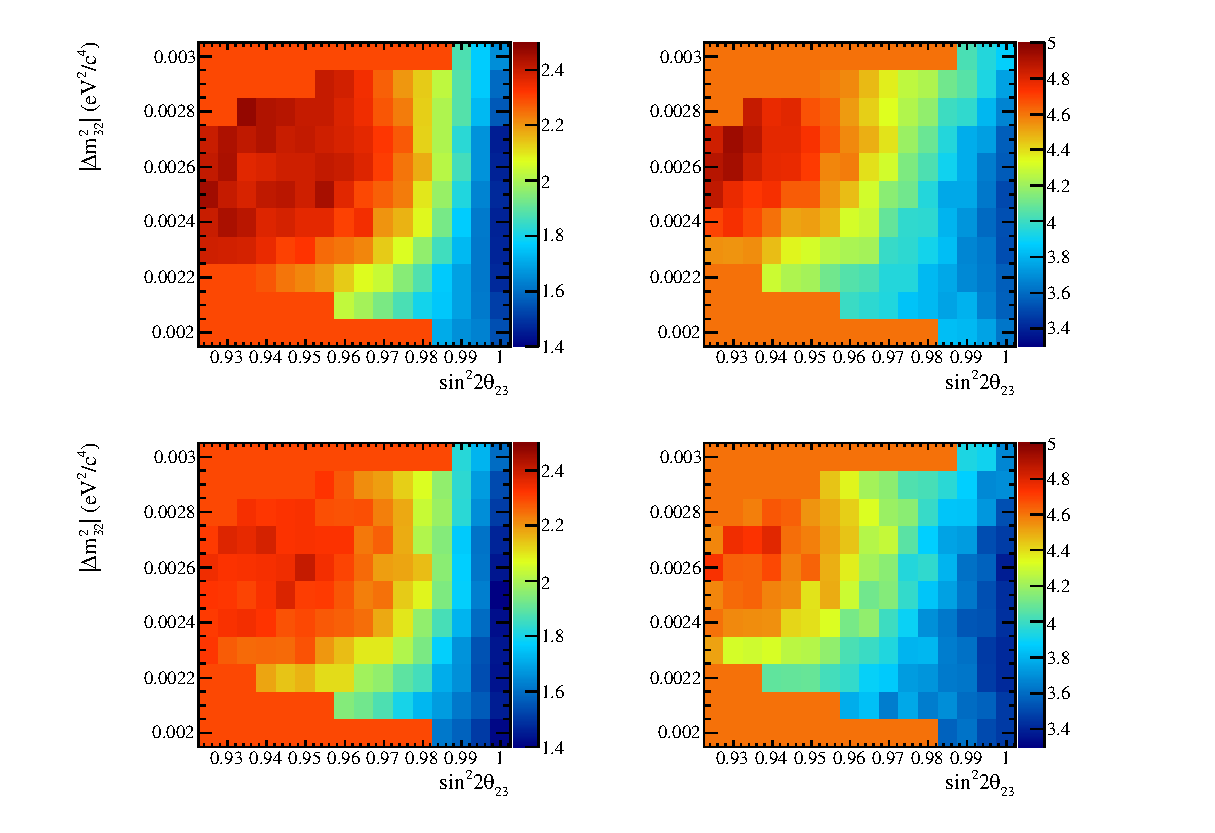
\includegraphics[width=42pc]{./images/feldman_cousins/FC_surfaces_28_2N.eps}
\caption {
  Monte Carlo estimation,
  according to the method of Feldman and Cousins,
  of $\Delta\chi^{2}_{critical}$ values $\Delta\chi^{2}_{68}$ (left) and $\Delta\chi^{2}_{90}$ (right)
  as functions of $\sin^{2}{2\theta_{23}}$ and $|\Delta{m^{2}_{32}}|$,
  for calculation of the 68\% and 90\% CL confidence regions
  for the 3.010 $\times$10$^{20}$-POT 3-flavour $\nu_{\mu}$-disappearance analysis.
  The top row shows $\Delta\chi^{2}_{critical}$ surfaces calculated using the `2+8' fit,
  whereas the bottom row shows surfaces calculated using the `2+N' fit.
  The surfaces were generated from an ensemble of toy-MC experiments including both
  randomized systematic variations and statistical fluctuations.
  As expected from \cite{FeldmanCousins}, the values of $\Delta\chi^{2}_{critical}$ 
  decrease as the physical boundary at $\sin^{2}{2\theta_{23}}$ = 1 is approached. 
}
\label{fig:fc_dchisqcrit_2d}
\end{figure*}

%.......

\begin{figure*}[htb]
\center
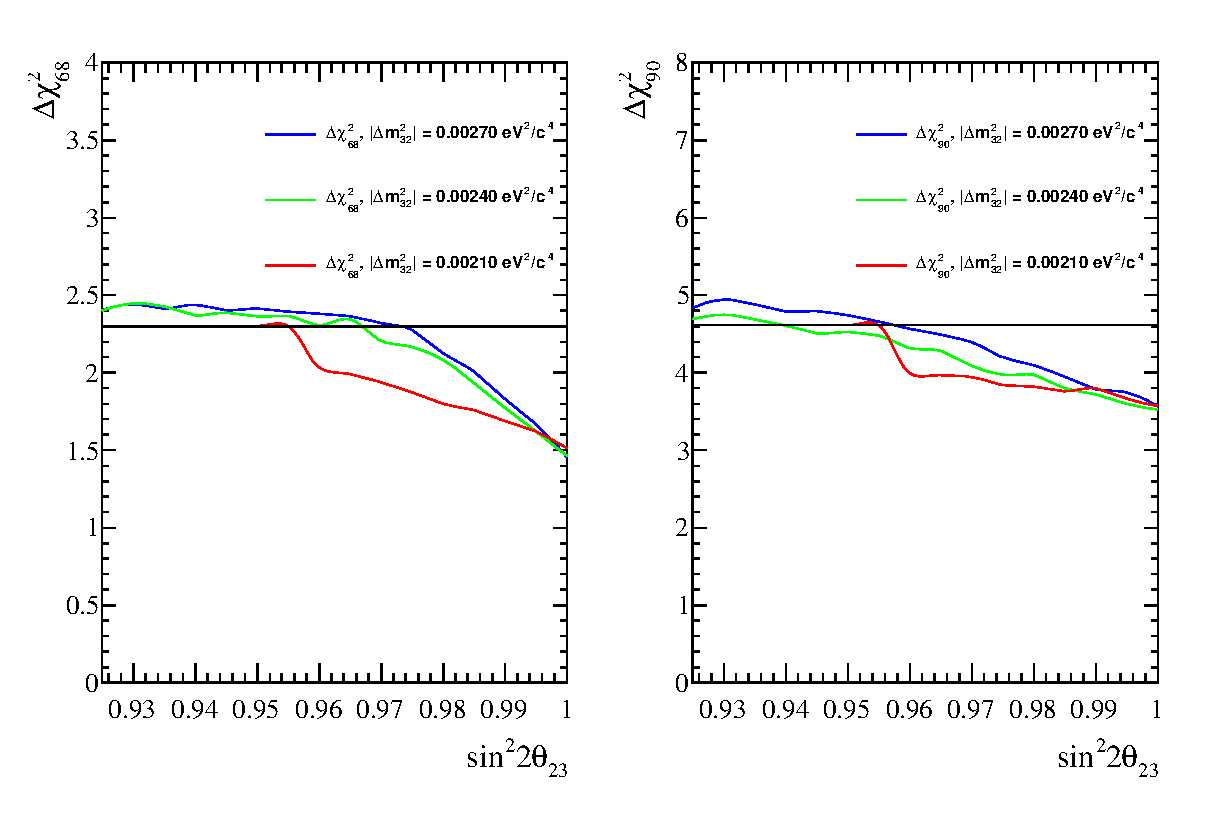
\includegraphics[width=30pc]{./images/feldman_cousins/FC_slice_mixing_28.eps}
\caption {
  Monte Carlo estimation,
  according to the method of Feldman and Cousins,
  of $\Delta\chi^{2}_{critical}$ values $\Delta\chi^{2}_{68}$ (left) and $\Delta\chi^{2}_{90}$ (right),
  as functions of $\sin^{2}{2\theta_{23}}$ for 3 different values of $|\Delta{m^{2}_{32}}|$
  (2.1$\times$10$^{-3}$ eV$^{2}/c^{4}$,
   2.4$\times$10$^{-3}$ eV$^{2}/c^{4}$ and
   2.7$\times$10$^{-3}$ eV$^{2}/c^{4}$).
  The $\Delta\chi^{2}_{critical}$ values were calculated
  from an ensemble of toy-MC experiments, for an exposure of 3.010$\times$10$^{20}$ POT, 
  including both randomized systematic variations and statistical fluctuations.
  The `2+8' fit was used.
  For comparison, the canonical value used in the constant $\Delta\chi^{2}_{critical}$
  method is also shown as a horizontal line.
}
\label{fig:fc_dchisqcrit_slice_mixing}
\end{figure*}

%.......

\begin{figure*}[htb]
\center
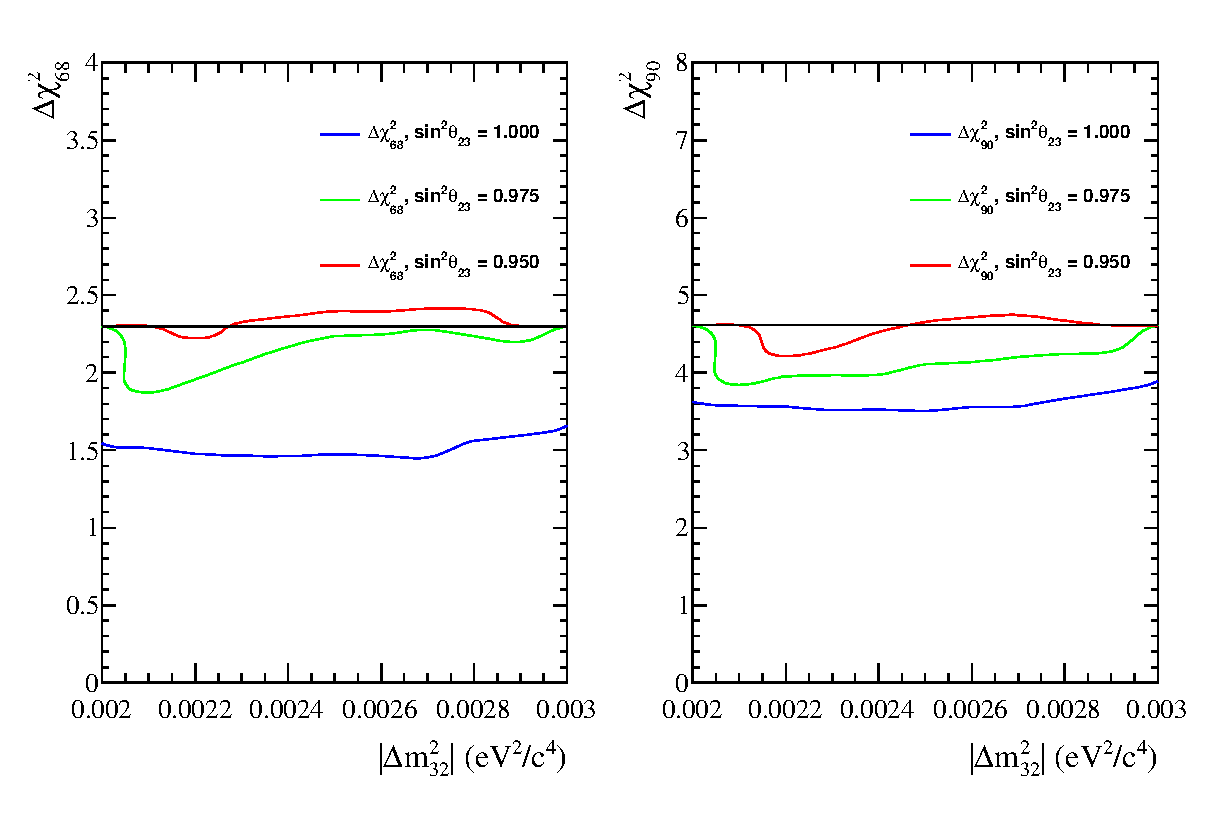
\includegraphics[width=30pc]{./images/feldman_cousins/FC_slice_dmsq_28.eps}
\caption {
  Monte Carlo estimation,
  according to the method of Feldman and Cousins,
  of $\Delta\chi^{2}_{critical}$ values $\Delta\chi^{2}_{68}$ (left) and $\Delta\chi^{2}_{90}$ (right),
  as functions of $|\Delta{m^{2}_{32}}|$ for 3 different values of $\sin^{2}{2\theta_{23}}$
  (0.950, 0.975 and 1.000).
  The $\Delta\chi^{2}_{critical}$ values were calculated
  from an ensemble of toy MC experiments, for an exposure of 3.010$\times$10$^{20}$ POT,
  including both randomized systematic variations and statistical fluctuations.
  The `2+8' fit was used.
  For comparison, the canonical value used in the constant $\Delta\chi^{2}_{critical}$
  method is also shown as a horizontal line.
}
\label{fig:fc_dchisqcrit_slice_dmsq}
\end{figure*}




\clearpage

\section {Results of the disappearance analysis with the Run 1+2+3 (3.010$\times10^{20}$ POT) dataset}
\label{sec:results}

%--------------------------------------------------------------------------------------
% Best-fit params & pulls
%--------------------------------------------------------------------------------------

\subsection {Best-fit oscillation parameters and systematic parameter pulls}
\label{sec:results_bestfit}

`2+N' and `2+8' 3-flavour $\nu_{\mu}$-disappearance fits were performed using the method described in 
section \ref{sec:oscfit} on the combined 3.010$\times$10$^{20}$ POT Run 1+2+3 dataset
and, separately, on the 1.431$\times$10$^{20}$ POT Run 1+2 and the 1.579$\times$10$^{20}$ POT Run 3 datasets.
The first octant is assumed for $\theta_{23}$ ($\sin(\theta_{23}) \leq 0.5$)
and the fit is for $\sin^22\theta_{23}$ and $|\Delta m^2_{32}|$ unless explicitly stated
otherwise.

Using the '2+N' fit for $\sin^2\theta_{23}$, this analysis found
$|\Delta m^{2}_{32}|$ = 2.441$\times$10$^{-3}$ $eV^{2}/c^{4}$ and
$\sin^{2}2\theta_{23}$ = 0.514
to be the best-fit values for the Run 1+2+3 dataset.

Using the `2+N' fit, this analysis found
$|\Delta m^{2}_{32}|$ = 2.443$\times$10$^{-3}$ $eV^{2}/c^{4}$ and
$\sin^{2}2\theta_{23}$ = 1.000
to be the best-fit values for the Run 1+2+3 dataset.
Similar best-fit values were obtained from separate `2+N' fits to subsets of the full dataset. A `2+N' fit 
to the Run 1+2 dataset gave best-fit values of $|\Delta m^{2}_{32}|$ = 2.588$\times$10$^{-3}$ $eV^{2}/c^{4}$ 
and $\sin^{2}2\theta_{23}$ = 0.986, while a fit to the Run 3 dataset gave $|\Delta m^{2}_{32}|$ = 
2.383$\times$10$^{-3}$ $eV^{2}/c^{4}$ and $\sin^{2}2\theta_{23}$ = 1.000).

Using the '2+N' fit, assuming that $\theta_{23}$ is in the second octant, yields a best-fit point almost identical to that assuming the
first octant; we found
$|\Delta m^{2}_{32}|$ = 2.441$\times$10$^{-3}$ $eV^{2}/c^{4}$ and
$\sin^{2}2\theta_{23}$ = 0.999.

The `2+8' fits produced results that are nearly identical to those from the `2+N' fits. Running the 
`2+8' fit on the combined Run 1+2+3 dataset, we found $|\Delta m^{2}_{32}|$ = 
2.442$\times$10$^{-3}$ $eV^{2}/c^{4}$ and $\sin^{2}2\theta_{23}$ = 1.000 as the best-fit values.
A `2+8' fit to the Run 1+2 dataset gave best-fit values of $|\Delta m^{2}_{32}|$ = 2.589$\times$10$^{-3}$ $eV^{2}/c^{4}$ 
and $\sin^{2}2\theta_{23}$ = 0.986, while a `2+8' fit to the Run 3 dataset gave $|\Delta m^{2}_{32}|$ = 
2.385$\times$10$^{-3}$ $eV^{2}/c^{4}$ and $\sin^{2}2\theta_{23}$ = 1.000.


The results of the fits are summarized in Tabs.\ \ref{tab:bestfit_sinsqtheta} and \ref{tab:data_fits:best_fit_values},
for fits to $\sin^2\theta_{23}$ and $\sin^22\theta_{23}$ respectively. In these tables are 
the best-fit oscillation parameters, the observed and expected number of single $\mu$-like ring events,
and the values of $\chi^{2}$ per degree of freedom at the best-fit.
The `2+N' and `2+8' fits give nearly identical best-fit values for the combined Run 1+2+3 dataset and, in fact,
for all running periods\footnote{
  It is interesting to know what the best-fit values would have been,
  had  $\sin^{2}(2\theta_{23})$ been allowed to enter into the unphysical region.
  This question can not be answered in a 3-flavour
  framework due to the existence of a $\sqrt{1-sin^{2}(2\theta_{23})}$ term in the oscillation probabilities,
  so we performed fits in a simple 2-flavour framework.
  In the presence of the physical boundary, a `2+8' fit to the Run 1+2+3 dataset 
  yields the following best-fit values:
  $\sin^{2}(2\theta_{23})$ = 1.000 and
  $|\Delta m^2_{32}| = 2.47 \times 10^{-3} eV^2/c^4$.
  If we do not constrain $\sin^{2}(2\theta_{23})$ within the physical region,
  the same fit yields the following best-fit values:
  $\sin^{2}(2\theta_{23})$ = 1.025 and
  $|\Delta m^2_{32}| = 2.47 \times 10^{-3} eV^2/c^4$.
}. Also the best-fit values are nearly identical between assuming the first octant and second octants for $\theta_{23}$ 
for the combined Run 1+2+3 dataset.

Using Eq.\ \ref{eqn:numusurv3fmin} and the value $\sin^2(2\theta_{13}) = 0.098$ used in this analysis,
the point of maximal disappeance occurs at $\sin^2(2\theta_{23}) = 0.999$ for the second octant, 
whilst the point of maximal disappearance is $\sin^2(2\theta_{23}) = 1.000$ for the first octant.
The result of the 2-flavour fit without the physical boundary show that the fit favours
a high amount of disappearance, more than is physically allowed in the 2-flavour framework.
Therefore it is not suprising that the '2+N' best-fit points' in the 3-flavour framework, are different,
and sit at the point of maximal disappearance, for the given octant assumption.

The pull for each systematic parameter f included in the fit, is calculated as
\begin{equation}
  \frac{f_{bf} - f_{nom}}{\sigma_{bf}},
  \label{eqn:bfpull}
\end{equation}
where 
$f_{bf}$ is the best-fit value of the systematic parameter,
$f_{nom}$ is the nominal value of the parameter (corresponding to no systematic variation), and
$\sigma_{bf}$ is the Hesse error output from Minuit.

The pulls of all 48 systematic parameters allowed to float in the `2+N' fit are shown in
Fig.\ \ref{fig:results_data123_pulls_2Nsintheta} for the fit to the Run 1+2+3 dataset using $\sin^2\theta_{23}$, in
Fig.\ \ref{fig:results_data123_pulls_2N} for the fit to the Run 1+2+3 dataset assuming the first octant for $\theta_{23}$, in
Fig.\ \ref{fig:results_data123_pulls_2NO2} for the fit to the Run 1+2+3 dataset assuming the second octant, and in 
Figs.\ \ref{fig:results_data12_pulls_2N}-\ref{fig:results_data3_pulls_2N} for the
fits to the Run 1+2 and Run 3 datasets.
From these figures, it is apparent that most systematic parameters barely move from their nominal values.
The pulls for the 8 dominant systematic parameters allowed to float in the `2+8' fit are shown in 
Fig.\ \ref{fig:results_data123_pulls} for the fit to the Run 1+2+3 dataset, and in 
Figs.\ \ref{fig:results_data12_pulls}-\ref{fig:results_data3_pulls} for the
fits to the Run 1+2 and Run 3 datasets.
The systematic parameter pulls shown in Fig.\ \ref{fig:results_data123_pulls_2N} for the `2+N' fit are 
similar to those in Fig.\ \ref{fig:results_data123_pulls} for the `2+8' fit.
The systematic parameter pulls shown in Fig.\ \ref{fig:results_data123_pulls_2NO2} for the `2+N' fit
assuming the second octant are 
similar to those in Fig.\ \ref{fig:results_data123_pulls_2N} for the `2+N' fit assuming the first octant.
For the `2+N' case, we note that, although all 48 systematic parameters are allowed to float in the fit,
only 6 of them move by more than $\pm$0.1$\sigma$, for either octant assumption, and when
fitting for $\sin^2\theta_{23}$.


%...........................................................
% Table summarizing best-fit results in sinsqtheta
%
\begin{table}
\centering
\begin{tabular}{| l | l | c | c | c  c | c | c | c |}
\hline
Analysis & sin$^2\theta_{23}$ & $\Delta m_{32}^2$ & N$_{obs}$ & N$_{exp}$ & $\chi^2_{bf} / ndf$ & p-value \\
\hline
3-flavour sin$^22\theta_{23}$ 1st octant & 0.500 &  2.443 $\cdot 10^{-3}$ & 58 & 57.97 & 56.04/71 & 0.83 \\
3-flavour sin$^22\theta_{23}$ 2nd octant & 0.516 &  2.441 $\cdot 10^{-3}$ & 58 & 57.92 & 56.03/71 & 0.82 \\
3-flavour sin$^2\theta_{23}$             & 0.514 &  2.441 $\cdot 10^{-3}$ & 58 & 57.92 & 56.03/71 & 0.80 \\
\hline
\end{tabular}
\caption{
  Summary of best-fit parameters for the combined Run 1+2+3 datasets
  for '2+N' fits with $\sin^22\theta_{23}$ converted to $\sin^2\theta_{23}$ (with both $\theta_{23}$ octant assumptions),
  and a '2+N' fit with $\sin^2\theta_{23}$.
  The quoted best-fit $\chi^2$ values ($\chi^2_{bf}$) were computed from Eq.\ \ref{eq:chisquare} 
  with the reconstructed energy binning used in each fit.
}
\label{tab:bestfit_sinsqtheta}
\end{table}

%...........................................................
%
% Table summarizing best-fit results
%
\begin{table}
\centering
\begin{tabular}{| l | l | c | c | c  c | c | c |}
\hline
Analysis & Run period & $\sin^22\theta_{23}$ & $\Delta m_{32}^2$ & N$_{obs}$ & N$_{exp}$ & $\chi^2_{bf} / ndf$ & p-value \\
\hline
2012 / 3-flavour 1st octant / `2+N' & Run 1+2+3 & 1.000 &  2.443 $\cdot 10^{-3}$ & 58 & 57.97 & 56.04/71 & 0.83 \\
2012 / 3-flavour 2nd octant / `2+N' & Run 1+2+3 & 0.999 &  2.441 $\cdot 10^{-3}$ & 58 & 57.92 & 56.03/71 & 0.82 \\
2012 / 3-flavour 1st octant / `2+8' & Run 1+2+3 & 1.000 &  2.442 $\cdot 10^{-3}$ & 58 & 57.92 & 56.15/71 & 0.82 \\
\hline
2012 / 3-flavour 1st octant / `2+N' & Run 3     & 1.000 &  2.383 $\cdot 10^{-3}$ & 27 & 29.58 & 56.28/71 & 0.83 \\
2012 / 3-flavour 1st octant / `2+8' & Run 3     & 1.000 &  2.385 $\cdot 10^{-3}$ & 27 & 29.60 & 56.32/71 & 0.63 \\
\hline
2012 / 3-flavour 1st octant / `2+N' & Run 1+2   & 0.986 &  2.588 $\cdot 10^{-3}$ & 31 & 29.04 & 38.96/71 & 0.82 \\
2012 / 3-flavour 1st octant / `2+8' & Run 1+2   & 0.986 &  2.589 $\cdot 10^{-3}$ & 31 & 29.04 & 39.06/71 & 0.68 \\
2010 / 2-flavour  / `2+0'           & Run 1+2   & 0.98  &  2.65  $\cdot 10^{-3}$ & 31 & 29.18 & 61.578/198  & - \\
\hline
\end{tabular}
\caption{
  Summary of best-fit parameters for the oscillation fits to the Run 1+2, Run 3, and combined Run 1+2+3 datasets. 
  Best-fit values are given for both $\theta_{23}$ octants.
  The 2010 result is taken from the analysis presented in \cite{OurRun12DisappAnalysis}.
  The quoted best-fit $\chi^2$ values ($\chi^2_{bf}$) were computed from Eq.\ \ref{eq:chisquare} 
  with the reconstructed energy binning used in each fit.
  The table also shows the p-values obtained from the goodness-of-fit test of Sec.\ \ref{sec:gof_test}
  for the `2+N' and `2+8' oscillation fits to the Run 1+2, Run 3, and combined Run 1+2+3 datasets. Again values are 
  given for both $\theta_{23}$ octants.
}
\label{tab:data_fits:best_fit_values}
\end{table}

%...........................................................
%
% Systematic parameter pulls for `2+N' fits
%

\begin{figure*}[htb]
\center
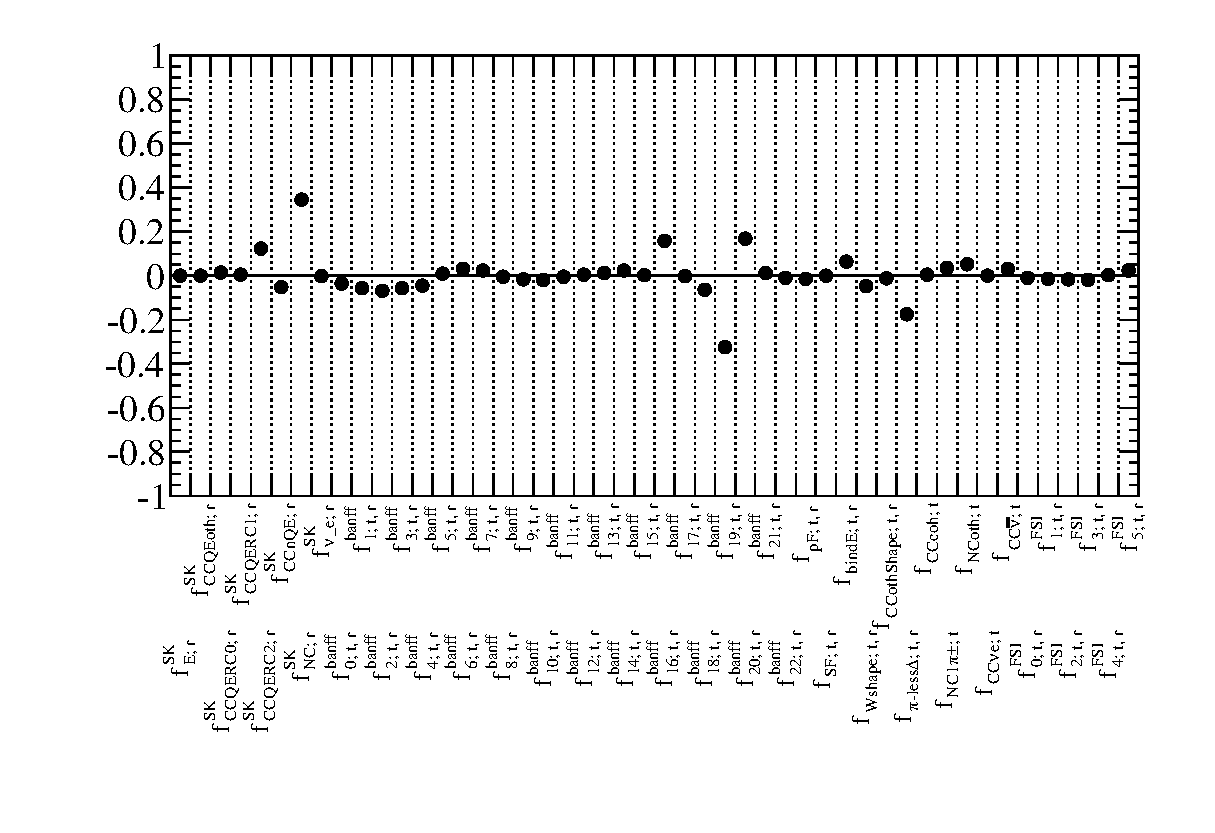
\includegraphics[width=50pc,angle=270]{./images/fit_data/2Nsintheta/pulls_3}
\caption {
  Systematic parameter pulls for the `2+N' $\sin^2\theta_{23}$ fit to the Run 1+2+3 dataset.
}
\label{fig:results_data123_pulls_2Nsintheta}
\end{figure*}

\begin{figure*}[htb]
\center
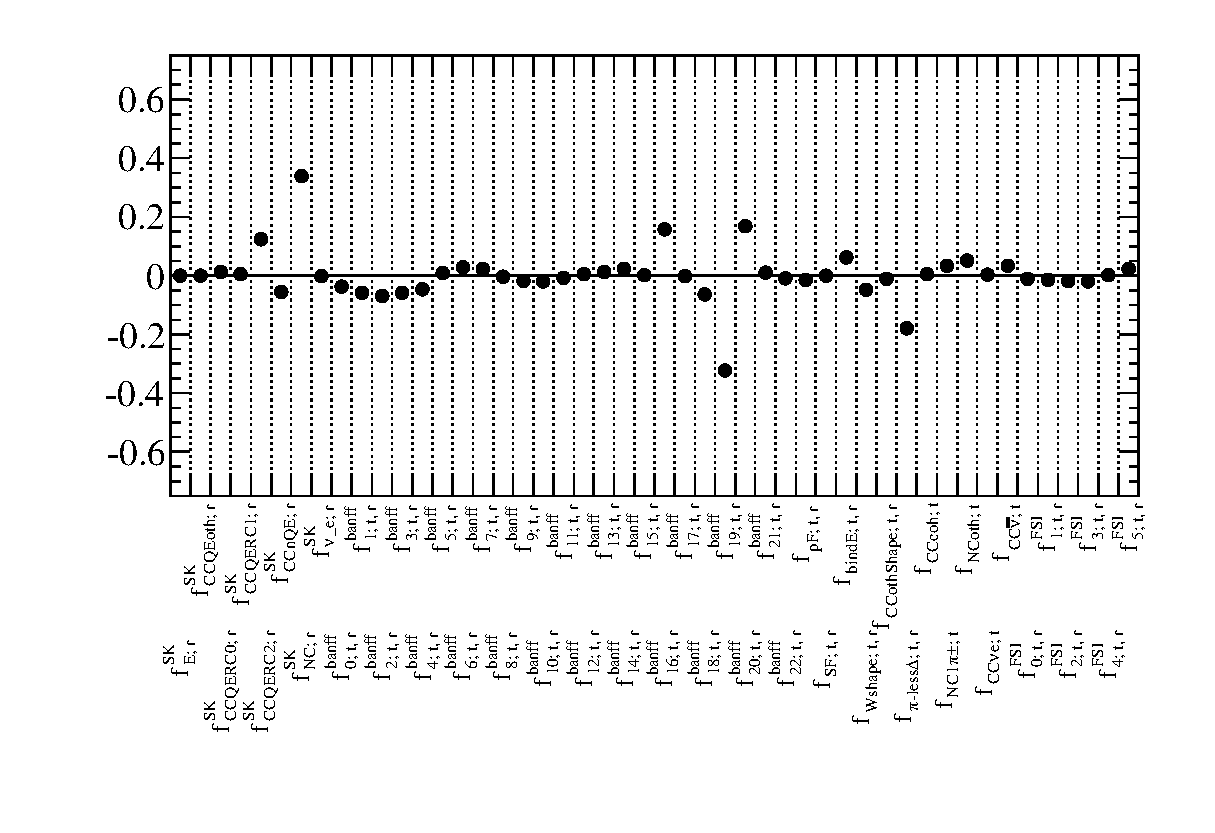
\includegraphics[width=50pc,angle=270]{./images/fit_data/2N/pulls_3}
\caption {
  Systematic parameter pulls for the `2+N' fit to the Run 1+2+3 dataset, assuming $\theta_{23}$ is in the first octant.
}
\label{fig:results_data123_pulls_2N}
\end{figure*}

\begin{figure*}[htb]
\center
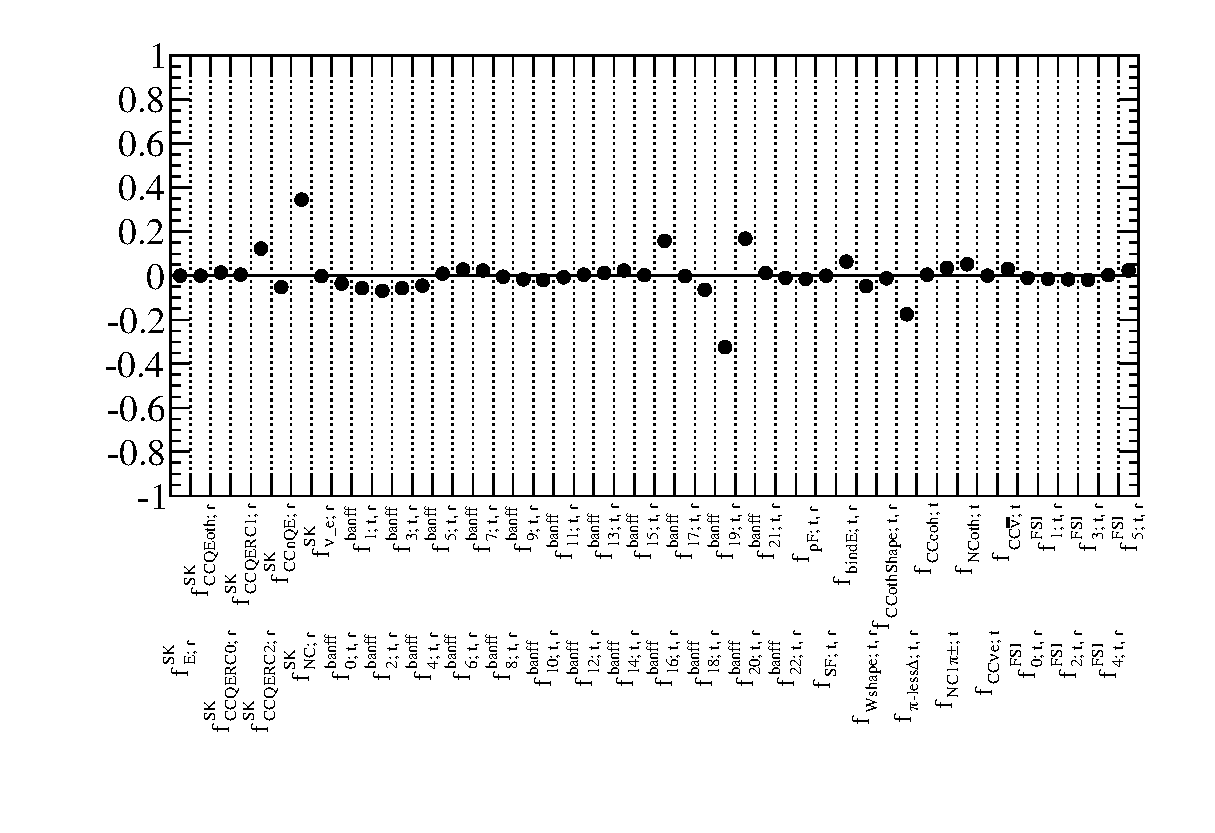
\includegraphics[width=50pc,angle=270]{./images/fit_data/2Noctant2/pulls_3}
\caption {
  Systematic parameter pulls for the `2+N' fit to the Run 1+2+3 dataset, assuming $\theta_{23}$ is in the second octant.
}
\label{fig:results_data123_pulls_2NO2}
\end{figure*}

\begin{figure*}[htb]
\begin{minipage}[t]{0.48\linewidth}
\center
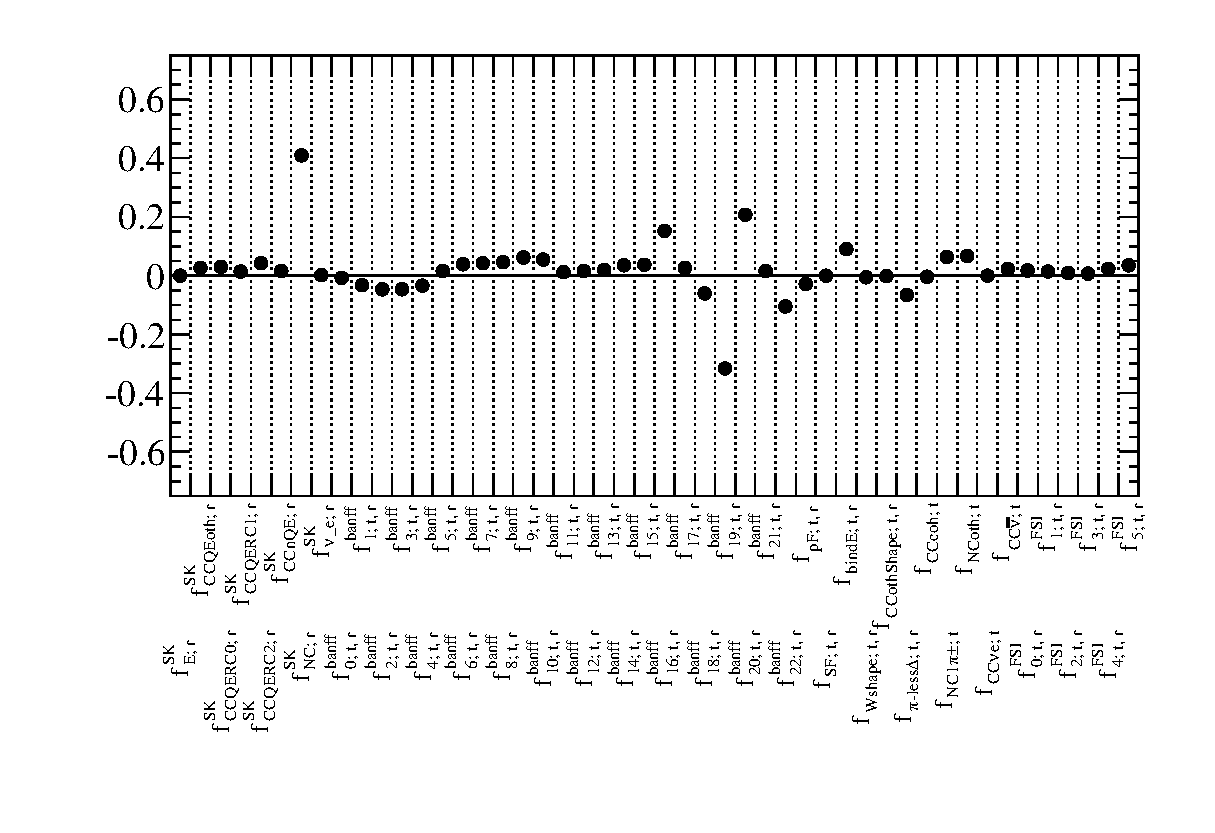
\includegraphics[width=22pc,angle=270]{./images/fit_data/2N/pulls_4}
\caption {
  Systematic parameter pulls for the `2+N' fit to the Run 1+2 dataset.
}
\label{fig:results_data12_pulls_2N}
\end{minipage}
\hspace{0.06\linewidth}
\begin{minipage}[t]{0.48\linewidth}
\center
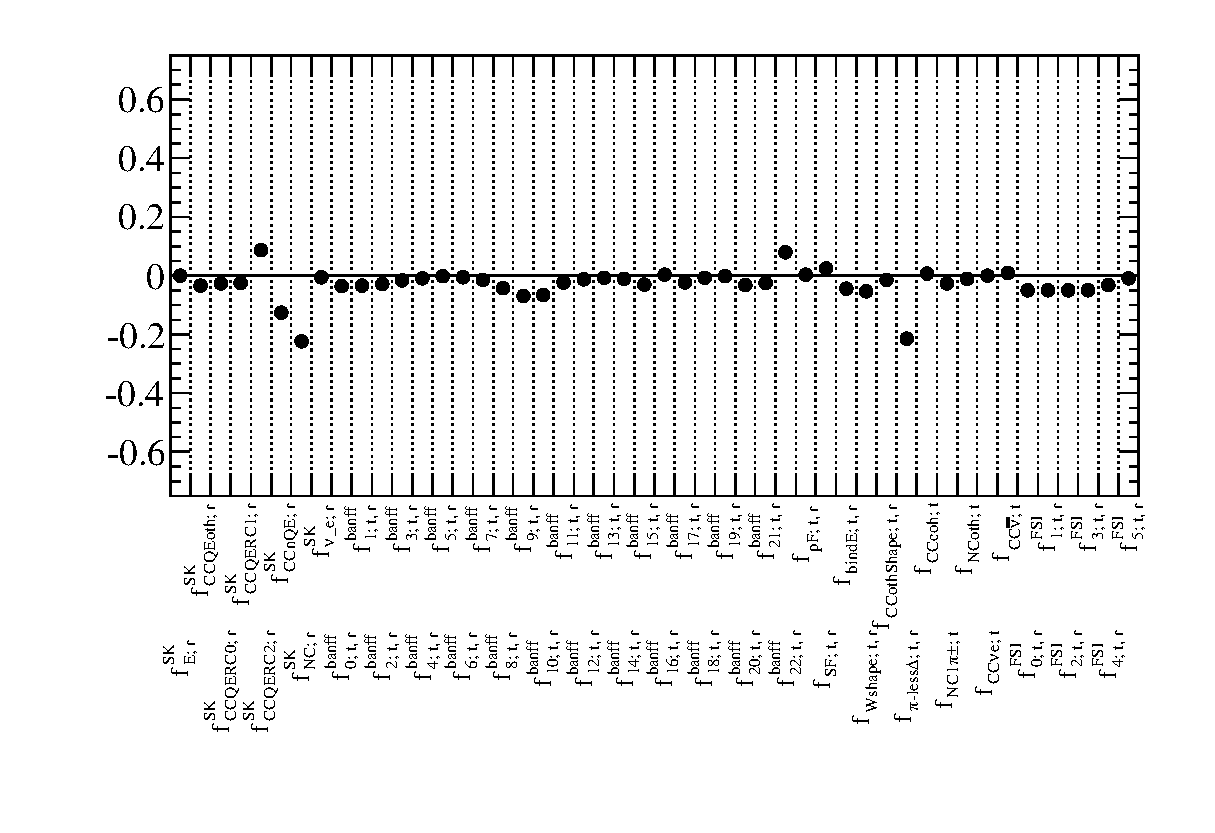
\includegraphics[width=22pc,angle=270]{./images/fit_data/2N/pulls_5}
\caption {
  Systematic parameter pulls for the `2+N' fit to the Run 3 dataset.
}
\label{fig:results_data3_pulls_2N}
\end{minipage}
\end{figure*}

%...........................................................
%
% Systematic parameter pulls for `2+8' fits
%
\clearpage
\begin{figure*}[htb]
\center
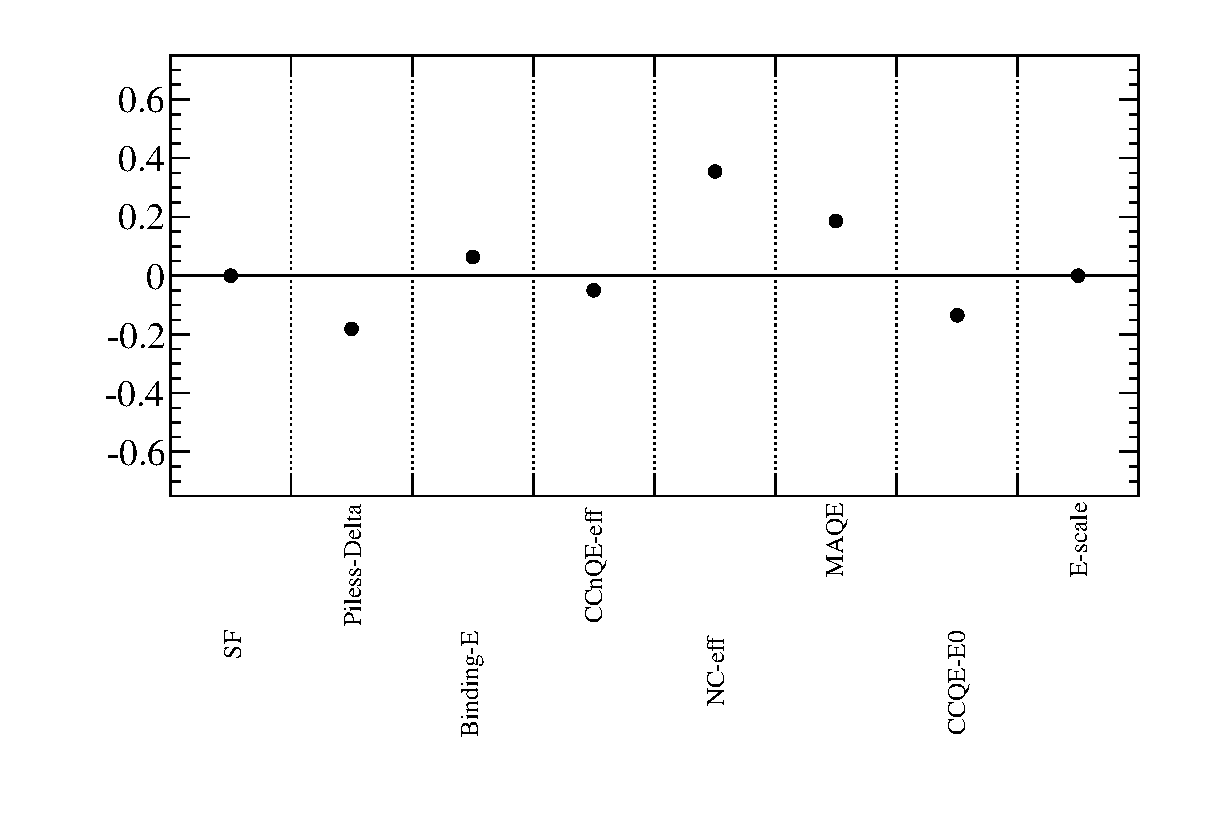
\includegraphics[width=25pc,angle=270]{./images/fit_data/28/pulls_3}
\caption {
  Systematic parameter pulls for the `2+8' fit to the Run 1+2+3 dataset.
}
\label{fig:results_data123_pulls}
\end{figure*}

\begin{figure*}[htb]
\begin{minipage}[t]{0.48\linewidth}
\center
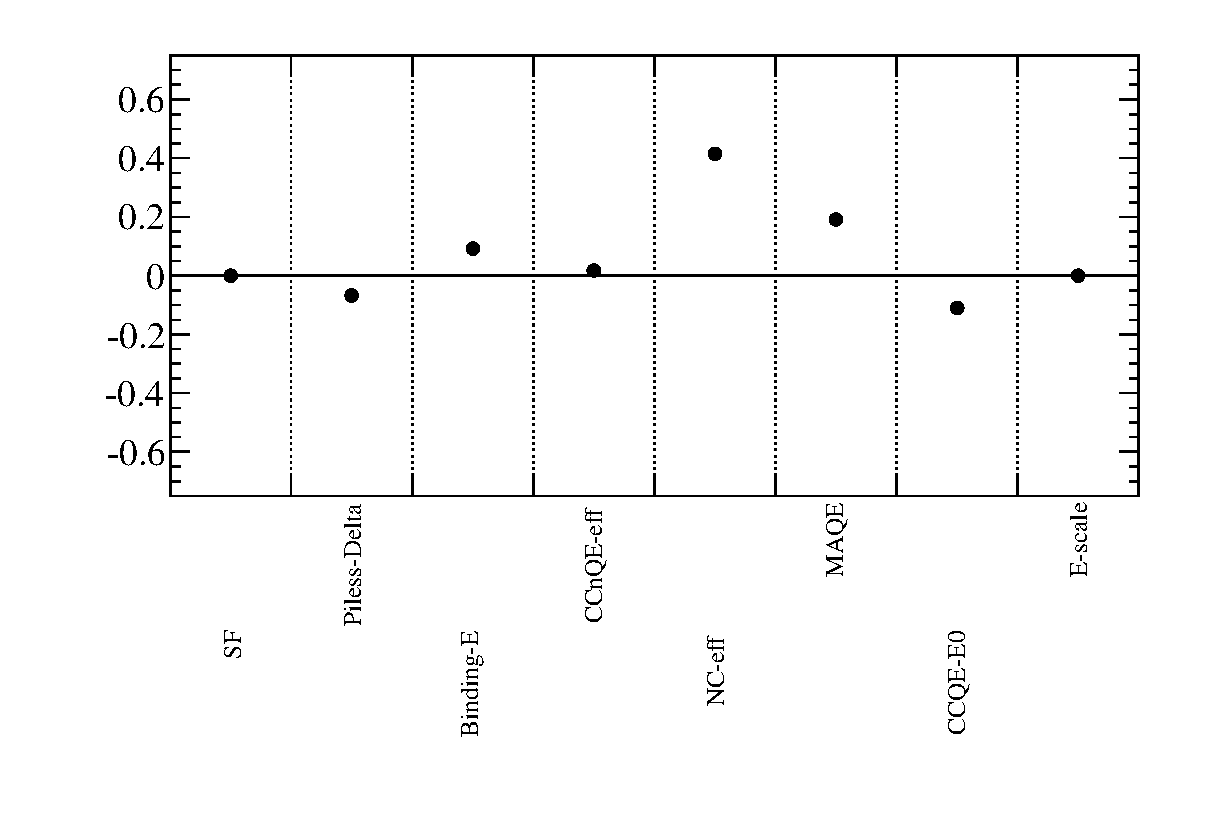
\includegraphics[width=20pc,angle=270]{./images/fit_data/28/pulls_4}
\caption {
  Systematic parameter pulls for the `2+8' fit to the Run 1+2 dataset.
}
\label{fig:results_data12_pulls}
\end{minipage}
\hspace{0.06\linewidth}
\begin{minipage}[t]{0.48\linewidth}
\center
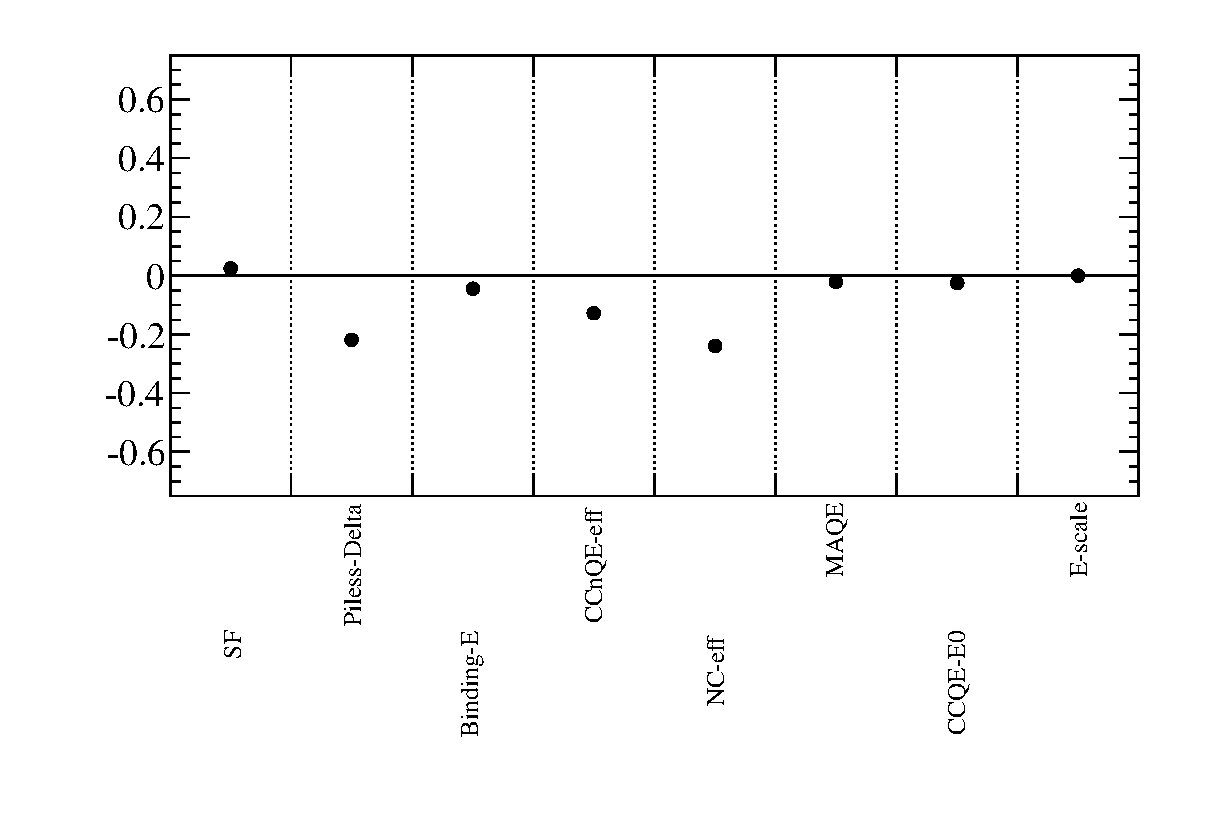
\includegraphics[width=20pc,angle=270]{./images/fit_data/28/pulls_5}
\caption {
  Systematic parameter pulls for the `2+8' fit to the Run 3 dataset.
}
\label{fig:results_data3_pulls}
\end{minipage}
\end{figure*}

%--------------------------------------------------------------------------------------
% Goodness of fit tests
%--------------------------------------------------------------------------------------

\clearpage
\subsection {Goodness-of-fit tests}
\label{sec:results_gof}

Goodness-of-fit tests were performed as described in Sec.\ \ref{sec:gof_test},
and the p-values for all `2+N' and `2+8' $\sin^22\theta_{23}$ fits to the Run 1+2+3, Run 1+2 and Run 3
datasets are shown in Tab.\ \ref{tab:data_fits:best_fit_values}. The $\chi^2$ distributions from 
which the p-values were calculated are shown for the `2+N' fit
for $\sin^2\theta_{23}$ in Fig.\ \ref{fig:results_data123_goodness_2Nsintheta},
for the '2+N' fit assuming the first and second octants for $\theta_{23}$ for
Run 1+2+3 data in Figs.\ \ref{fig:results_data123_goodness_2N} and \ref{fig:results_data123_goodness_2NO2} respectively,
and for the '2+8' fit for Run 1+2+3 data in Fig.\ \ref{fig:results_data123_goodness}.
All fits have a high degree of plausibility.

%..................................
%
% Summary table with fit p-values
%
%\begin{table}
%\centering
%\begin{tabular}{| l | l | c |}
%\hline
%Analysis                 & Run period & p-value \\
%\hline
%2012 / 3-flavour / `2+N' & Run 1+2+3   & 0.83 \\
%2012 / 3-flavour / `2+8' & Run 1+2+3   & 0.82 \\
%\hline
%2012 / 3-flavour / `2+N' & Run 3       & 0.83 \\
%2012 / 3-flavour / `2+8' & Run 3       & 0.63 \\
%\hline
%2012 / 3-flavour / `2+N' & Run 1+2     & 0.82 \\
%2012 / 3-flavour / `2+8' & Run 1+2     & 0.68 \\
%\hline
%\end{tabular}
%\caption{
%  Summary of p-values obtained from the goodness-of-fit test of Sec.\ \ref{sec:gof_test}
%  for both `2+N' and `2+8' oscillation fits to the Run 1+2, Run 3, and combined Run 1+2+3 datasets.
%}
%\label{tab:data_fit:gof}
%\end{table}
%


%..................................
%
% Chisq_{gof} distributions
%

\begin{figure*}[htb]
\begin{minipage}[t]{0.48\linewidth}
\center
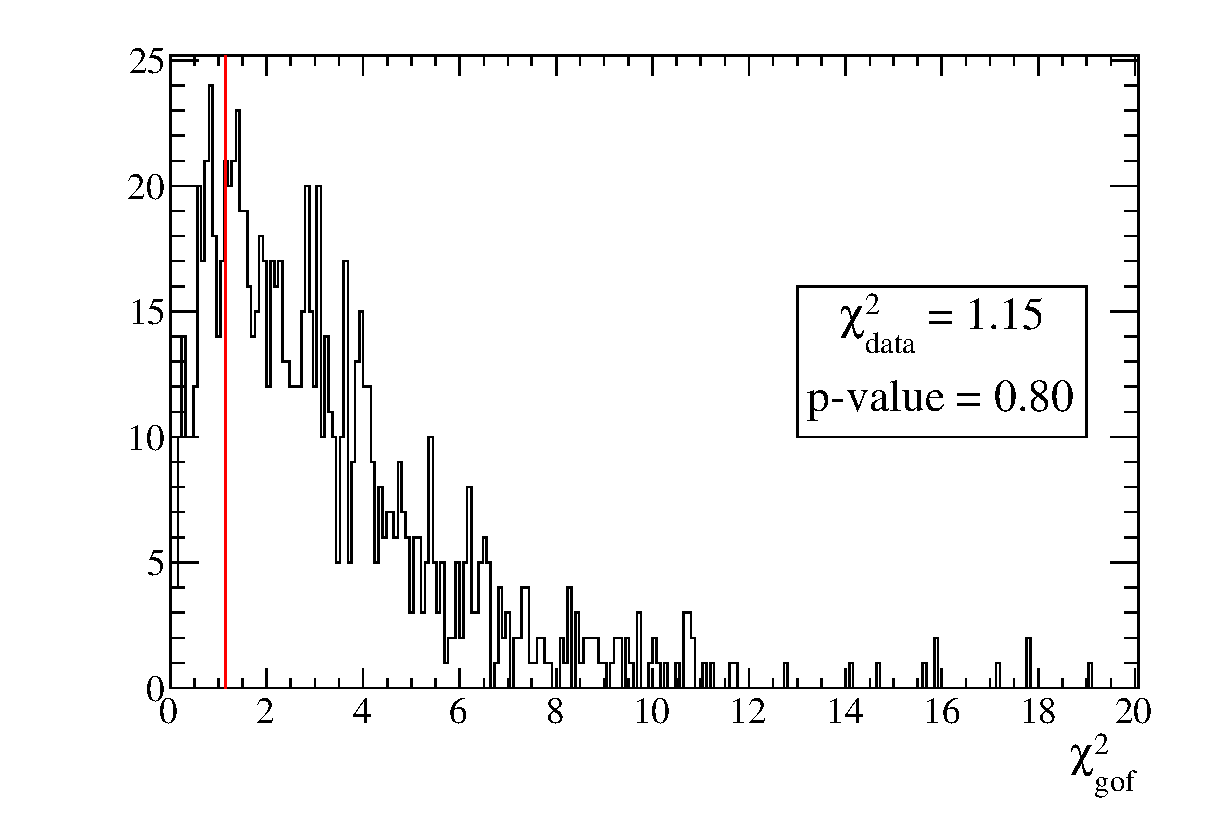
\includegraphics[width=18pc]{./images/fit_data/2Nsintheta/goodness_3}
\caption {
  Distribution of $\chi^2_{gof}$, the goodness-of-fit (gof) $\chi^2$, 
  from 1k toy MC experiments generated at the `2+N' $\sin^2\theta_{23}$ Run 1+2+3 best-fit oscillation point.
  The $\chi^2_{gof}$ value for the Run 1+2+3 data ($\chi^2_{data}$) is highlighted.
}
\label{fig:results_data123_goodness_2Nsintheta}
\end{minipage}
\hspace{0.06\linewidth}
\begin{minipage}[t]{0.48\linewidth}
\center
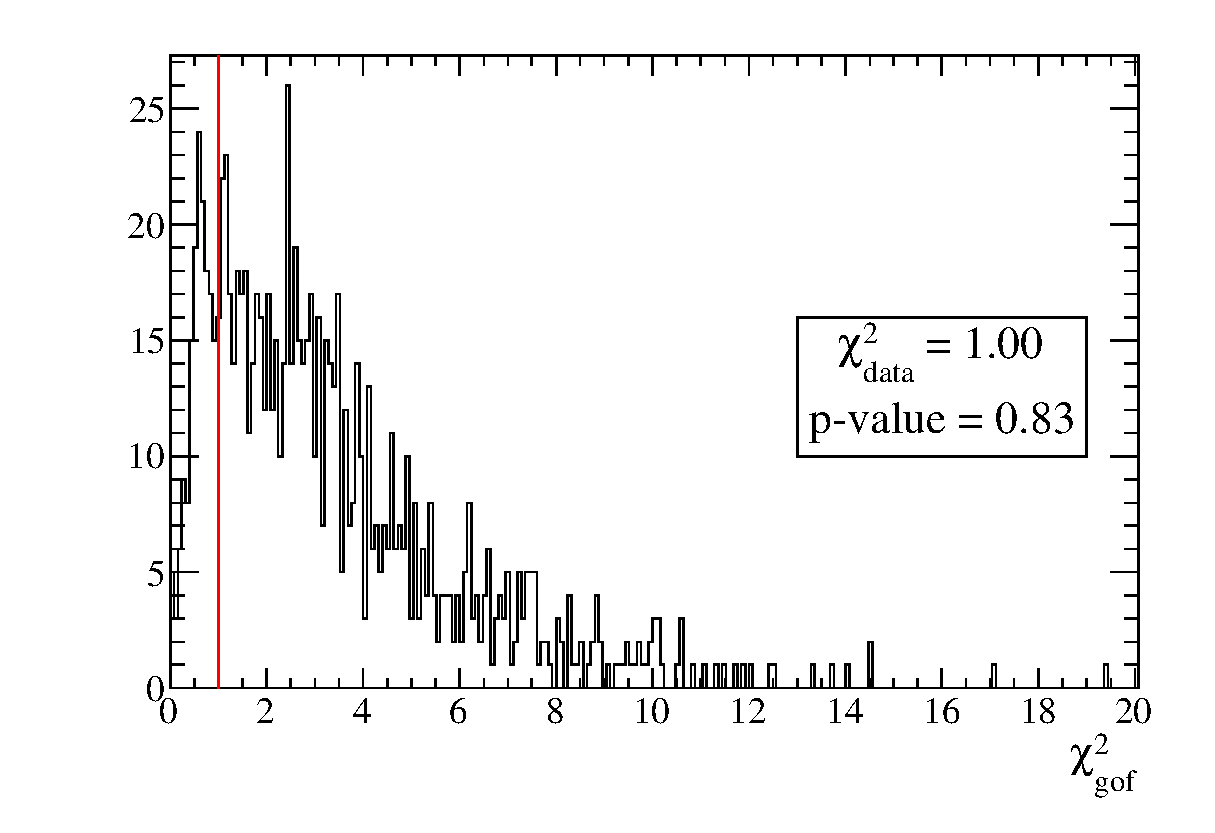
\includegraphics[width=18pc]{./images/fit_data/2N/goodness_3}
\caption {
  As in Fig.\ \ref{fig:results_data123_goodness_2Nsintheta}, but for the `2+N' fit to the Run 1+2+3 dataset
  assuming $\theta_{23}$ is in the first octant.
}
\label{fig:results_data123_goodness_2N}
\end{minipage}
\end{figure*}


\begin{figure*}[htb]
\begin{minipage}[t]{0.48\linewidth}
\center
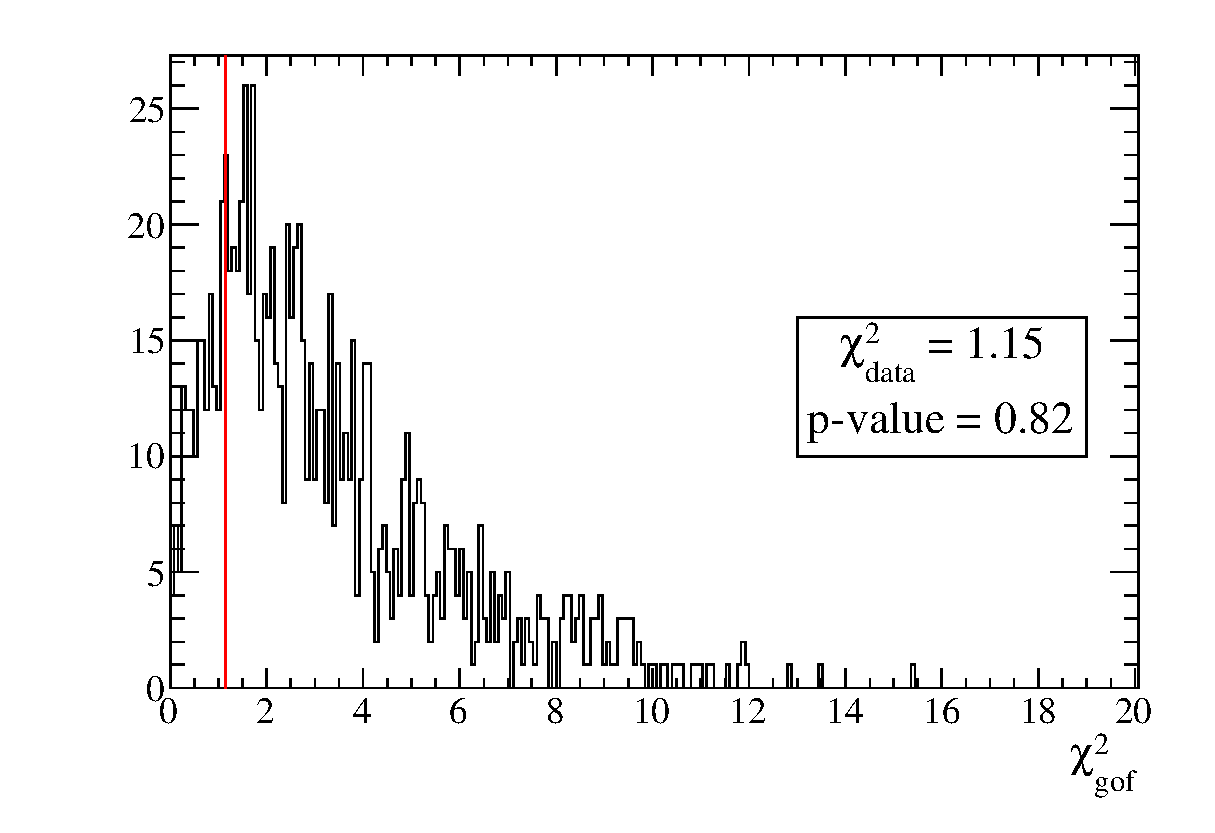
\includegraphics[width=18pc]{./images/fit_data/2Noctant2/goodness_3}
\caption {
  As in Fig.\ \ref{fig:results_data123_goodness_2Nsintheta}, but for the `2+N' fit to the Run 1+2+3 dataset
  assuming $\theta_{23}$ is in the second octant.
}
\label{fig:results_data123_goodness_2NO2}
\end{minipage}
\hspace{0.06\linewidth}
\begin{minipage}[t]{0.48\linewidth}
\center
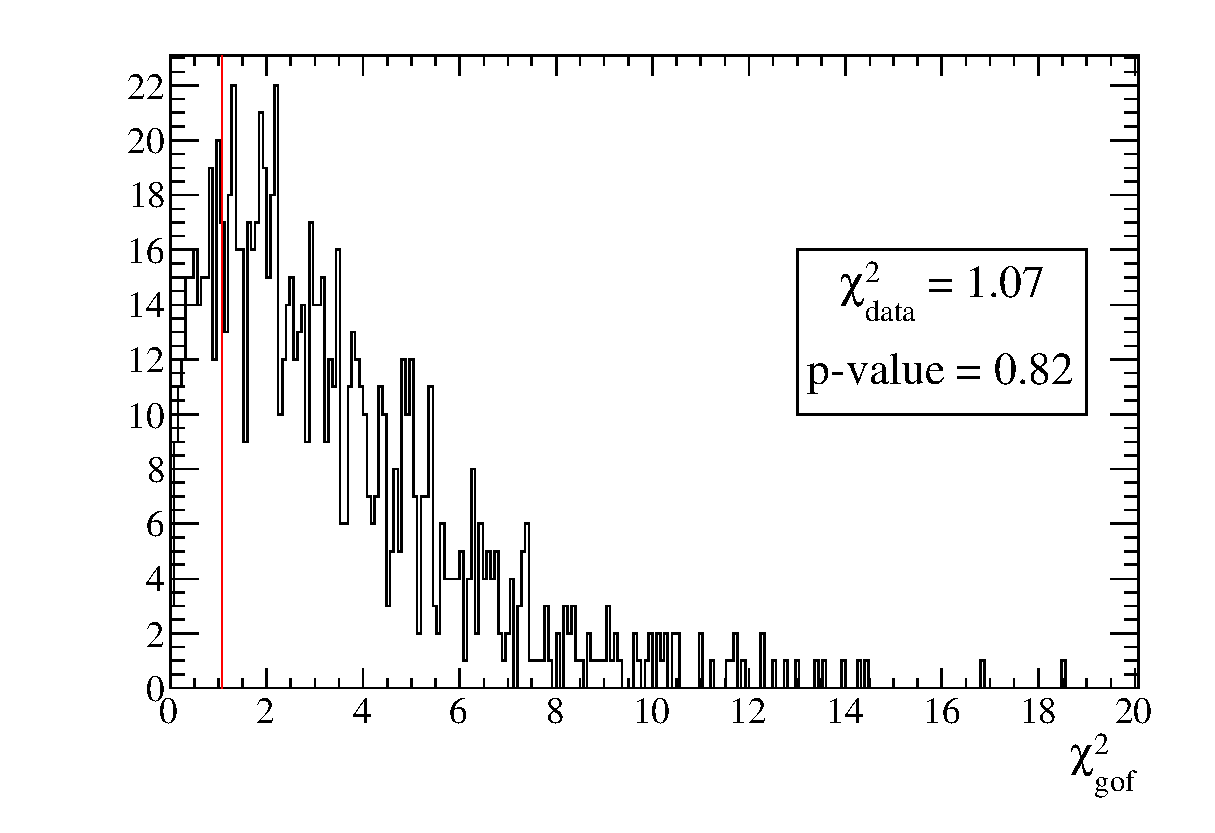
\includegraphics[width=18pc]{./images/fit_data/28/goodness_3}
\caption {
  As in Fig.\ \ref{fig:results_data123_goodness_2Nsintheta}, but for the `2+8' fit to the Run 1+2+3 dataset.
}
\label{fig:results_data123_goodness}
\end{minipage}
\end{figure*}


%--------------------------------------------------------------------------------------
% Best-fit spectra
%--------------------------------------------------------------------------------------

\subsection {Best-fit single $\mu$-like ring reconstructed energy spectra}
\label{sec:results_bestfit_spectra}

The reconstructed neutrino energy distribution of the single $\mu$-like ring events in the Run 1+2+3 dataset is shown in Fig.\ 
\ref{fig:results_data123_spectrum_2Nsintheta} along with the `2+N' $\sin^2\theta_{23}$ best-fit prediction and
the prediction made under the no-oscillation 
hypothesis. Also shown is the ratio between the data and the no-oscillation spectrum and the ratio between the `2+N' $\sin^2\theta_{23}$ best-fit 
spectrum and the the no-oscillation spectrum; in both of these ratios, the characteristic energy-dependent deficit can be 
clearly seen.
The equivalent spectra for the Run 1+2+3 (assuming $\theta_{23}$ is in the first octant),
Run 1+2+3 (assuming $\theta_{23}$ is in the second octant),
Run 1+2 and Run 3 datasets are also shown in Figs.\ \ref{fig:results_data123_spectrum_2N}, \ref{fig:results_data123_spectrum_2NO2}, \ref{fig:results_data12_spectrum_2N} 
and \ref{fig:results_data3_spectrum_2N} respectively. All these distribution are shown in the 73-bin scheme in reconstructed 
neutrino energy that was used in the fitting procedure (see Sec.\ \ref{sec:mc_templates:template_binning}).

`2+8' fits were also made to the Run 1+2+3, Run 1+2 and Run 3 datasets. The best-fit and no-oscillation spectra are compared with 
the data in in Figs.\
\ref{fig:results_data123_spectrum},  
\ref{fig:results_data12_spectrum} and
\ref{fig:results_data3_spectrum}.
The ratios of the data and best-fit spectra to the no-oscillation spectra are also shown in these figures, and the energy-dependent 
deficits are once more clearly visible. 

Since the reconstructed energy binning used in the fit is relatively fine, it can be beneficial to see the above distributions using 
a coarser binning. The best-fit spectra obtained for the Run 1+2+3 dataset from the `2+N' fit for $\sin^2\theta_{23}$,
the '2+N' fit with $\theta_{23}$ in the first octant, 
the '2+N' fit with $\theta_{23}$ in the second octant and the `2+8' fit with $\theta_{23}$ in the first octant are shown using a coarse 
binning\footnote{
  16 reconstructed energy bins arranged as follows:
  1 0.3-GeV bin in 0 - 0.3 GeV,
  8 0.1-GeV bins in 0.3 - 1.1 GeV,
  1 0.15-GeV bin in 1.1 GeV - 1.25 GeV,
  1 0.25-GeV bin in 1.25 - 1.5 GeV GeV,
  1 0.5-GeV bin in 1.5 - 2 GeV,
  2 1-GeV bin in 2-4 GeV,
  1 2-GeV bin in 4-6 GeV and 1 bin above 6 GeV.
} 
in Figs.\
\ref{fig:results_data123_spectrum_coarse_2Nsintheta},
\ref{fig:results_data123_spectrum_coarse_2N},
\ref{fig:results_data123_spectrum_coarse_2NO2} and
\ref{fig:results_data123_spectrum_coarse}
respectively. It is also interesting to see the 28 components of the best-fit spectrum, each of which is calculated separately 
in this analysis. These components are shown for the `2+N' and `2+8' 
fits in Figs.\ 
\ref{fig:results_data123_spectrum_components_2Nsintheta},
\ref{fig:results_data123_spectrum_components_2N},
\ref{fig:results_data123_spectrum_components_2NO2} and
\ref{fig:results_data123_spectrum_components} respectively.
In these plots, the components of the spectrum are grouped into 5 categories: 
$\nu_{\mu}$ CCQE, $\nu_{\mu}$ CCnonQE, $\bar{\nu}_{\mu}$ CC, $\nu_{e}$/$\bar{\nu}_{e}$ CC and NC.

The '2+N' best-fit predictions for $\sin^2\theta_{23}$ and $\theta_{23}$ assuming the second octant
are compared for the Run 1+2+3 dataset only in  
Fig.\ \ref{fig:results_data123_spectrum_comparison_sintheta}, 
using the 73 reconstructed energy bins used in the fit, and in
Fig.\ \ref{fig:results_data123_spectrum_comparison_sintheta_coarse},
using the coarser binning described above.
The two best-fit spectra are nearly identical. In the 73-bin scheme used for the fit,
the spectra never differ by more than 0.1\% in the area below 3 GeV,
and they are nearly identical in the area of the first oscillation maximum.

The '2+N' best-fit predictions for both $\theta_{23}$ octant assumptions are compared for the Run 1+2+3 dataset only in  
Fig.\ \ref{fig:results_data123_spectrum_comparison_octant}, 
using the 73 reconstructed energy bins used in the fit, and in
Fig.\ \ref{fig:results_data123_spectrum_comparison_octant_coarse},
using the coarser binning described above.

Finally, the `2+N' and `2+8' best-fit predictions are compared for the Run 1+2+3 dataset only in  
Fig.\ \ref{fig:results_data123_spectrum_comparison}, 
using the 73 reconstructed energy bins used in the fit, and in
Fig.\ \ref{fig:results_data123_spectrum_comparison_coarse},
using the coarser binning described above.
The two best-fit spectra are nearly identical. In the 73-bin scheme used for the fit,
the spectra never differ by more than 1.5\% in the area below 3 GeV,
and they are nearly identical in the area of the first oscillation maximum.

%...........................................................
%
% Best-fit spectra and ratios for `2+N' fits (73 bins)
%
\begin{figure*}[htb]
\center
\includegraphics[width=28pc]{./images/fit_data/2Nsintheta/spectrum_3}
\caption {
  Best-fit reconstructed energy spectrum (top) obtained from the `2+N' $\sin^2\theta_{23}$ fit to the combined Run 1+2+3 dataset.
  The Run 1+2+3 dataset and the prediction obtained from the no-oscillation hypothesis are also shown.
  The spectra are shown using the 73 bins used in the fit (see Sec.\ \ref{sec:mc_templates:template_binning}).
  The ratio of the data and best-fit distribution to the no-oscillation hypothesis is shown 
  in the bottom plot. The characteristic energy-dependent deficit can be clearly seen.
}
\label{fig:results_data123_spectrum_2Nsintheta}
\end{figure*}

\begin{figure*}[htb]
\center
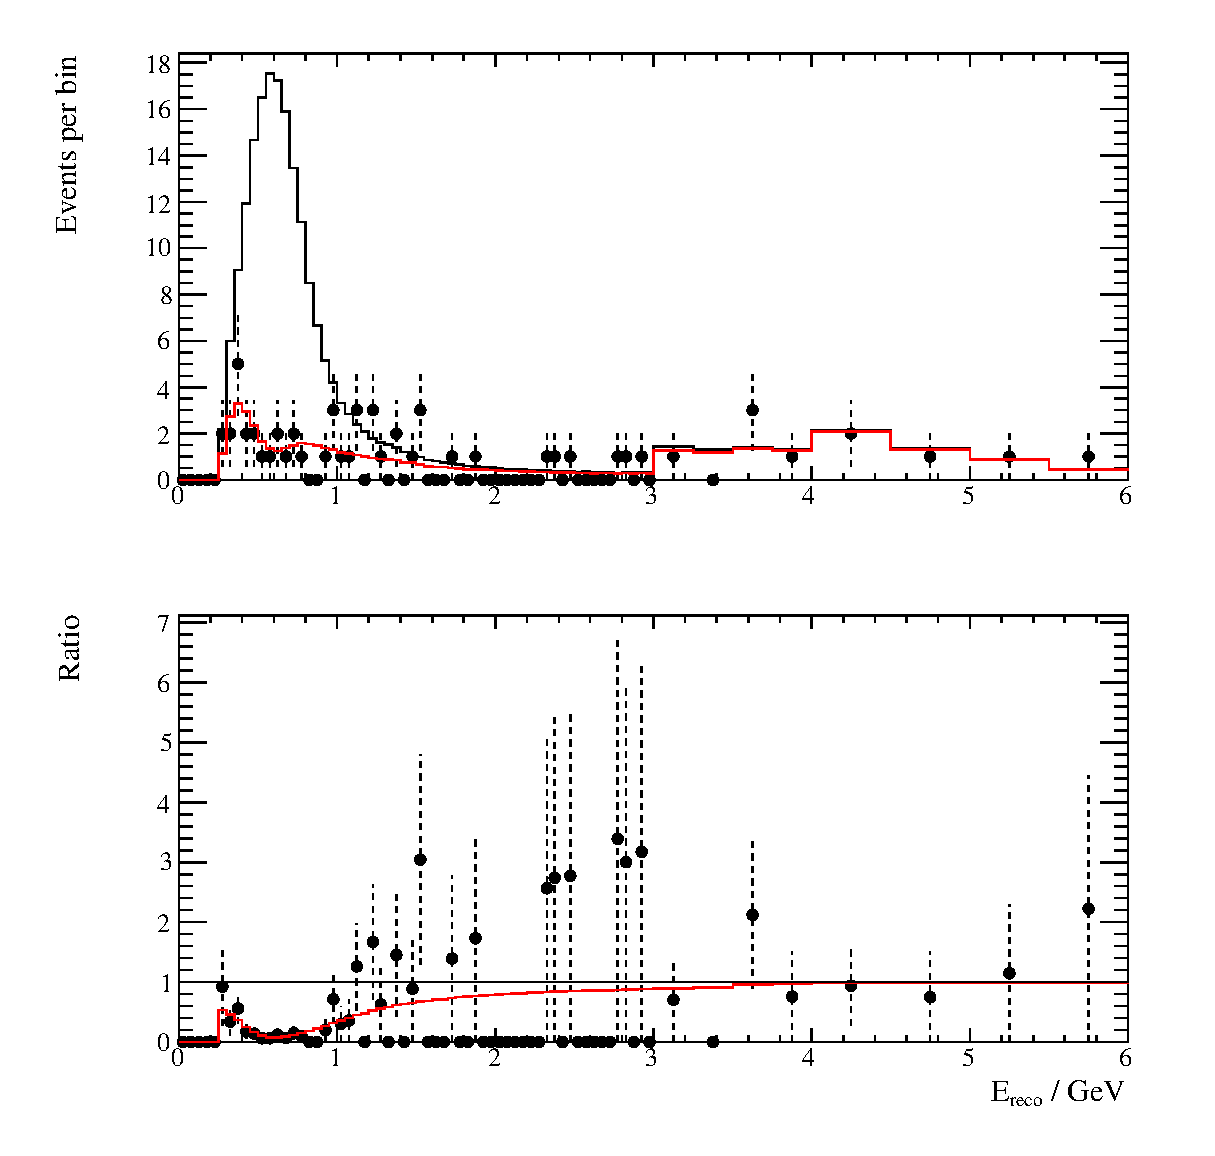
\includegraphics[width=28pc]{./images/fit_data/2N/spectrum_3}
\caption {
  Best-fit reconstructed energy spectrum (top) obtained from the `2+N' fit to the combined Run 1+2+3 dataset.
  The Run 1+2+3 dataset and the prediction obtained from the no-oscillation hypothesis are also shown.
  The spectra are shown using the 73 bins used in the fit (see Sec.\ \ref{sec:mc_templates:template_binning}).
  The ratio of the data and best-fit distribution to the no-oscillation hypothesis is shown 
  in the bottom plot. The characteristic energy-dependent deficit can be clearly seen.
}
\label{fig:results_data123_spectrum_2N}
\end{figure*}

\begin{figure*}[htb]
\center
\includegraphics[width=28pc]{./images/fit_data/2Noctant2/spectrum_3}
\caption {
  Best-fit reconstructed energy spectrum (top) obtained from the `2+N' fit to the combined Run 1+2+3 dataset,
  assuming $\theta_{23}$ is in the second octant.
  The Run 1+2+3 dataset and the prediction obtained from the no-oscillation hypothesis are also shown.
  The spectra are shown using the 73 bins used in the fit (see Sec.\ \ref{sec:mc_templates:template_binning}).
  The ratio of the data and best-fit distribution to the no-oscillation hypothesis is shown 
  in the bottom plot. The characteristic energy-dependent deficit can be clearly seen.
}
\label{fig:results_data123_spectrum_2NO2}
\end{figure*}

\begin{figure*}[htb]
\begin{minipage}[t]{0.48\linewidth}
\center
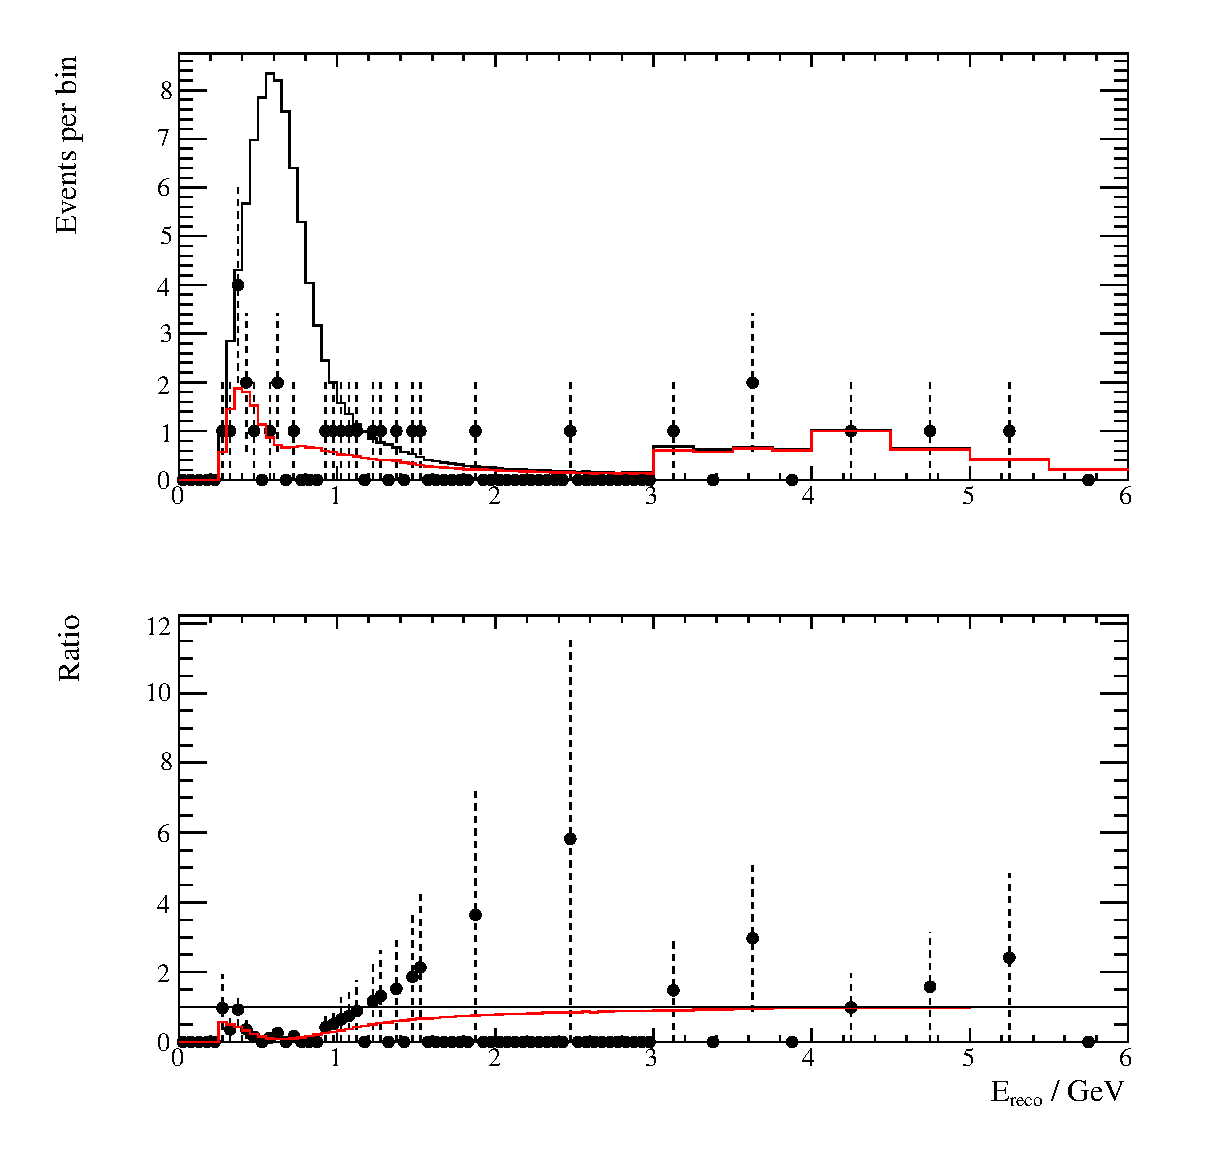
\includegraphics[width=20pc]{./images/fit_data/2N/spectrum_4}
\caption {
  As in Fig.\ \ref{fig:results_data123_spectrum_2N}, but for the Run 1+2 dataset only.
}
\label{fig:results_data12_spectrum_2N}
\end{minipage}
\hspace{0.06\linewidth}
\begin{minipage}[t]{0.48\linewidth}
\center
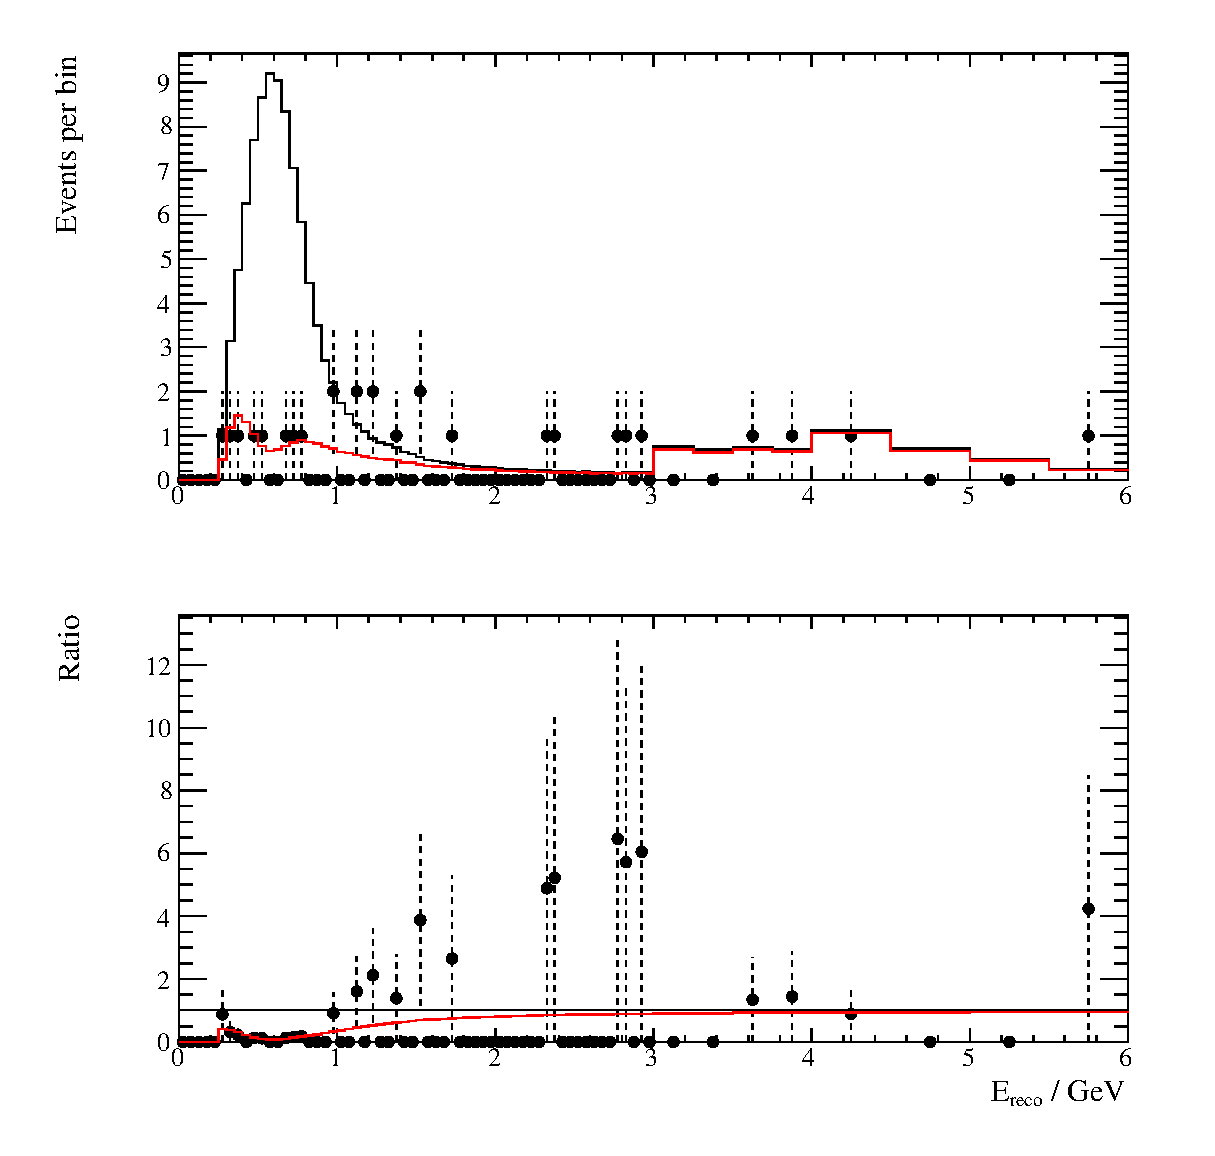
\includegraphics[width=20pc]{./images/fit_data/2N/spectrum_5}
\caption {
  As in Fig.\ \ref{fig:results_data123_spectrum_2N}, but for the Run 3 dataset only.
}
\label{fig:results_data3_spectrum_2N}
\end{minipage}
\end{figure*}


% ...........................................................
%
% Best-fit spectra and ratios for `2+8' fits (73 bins)
%
\begin{figure*}[htb]
\center
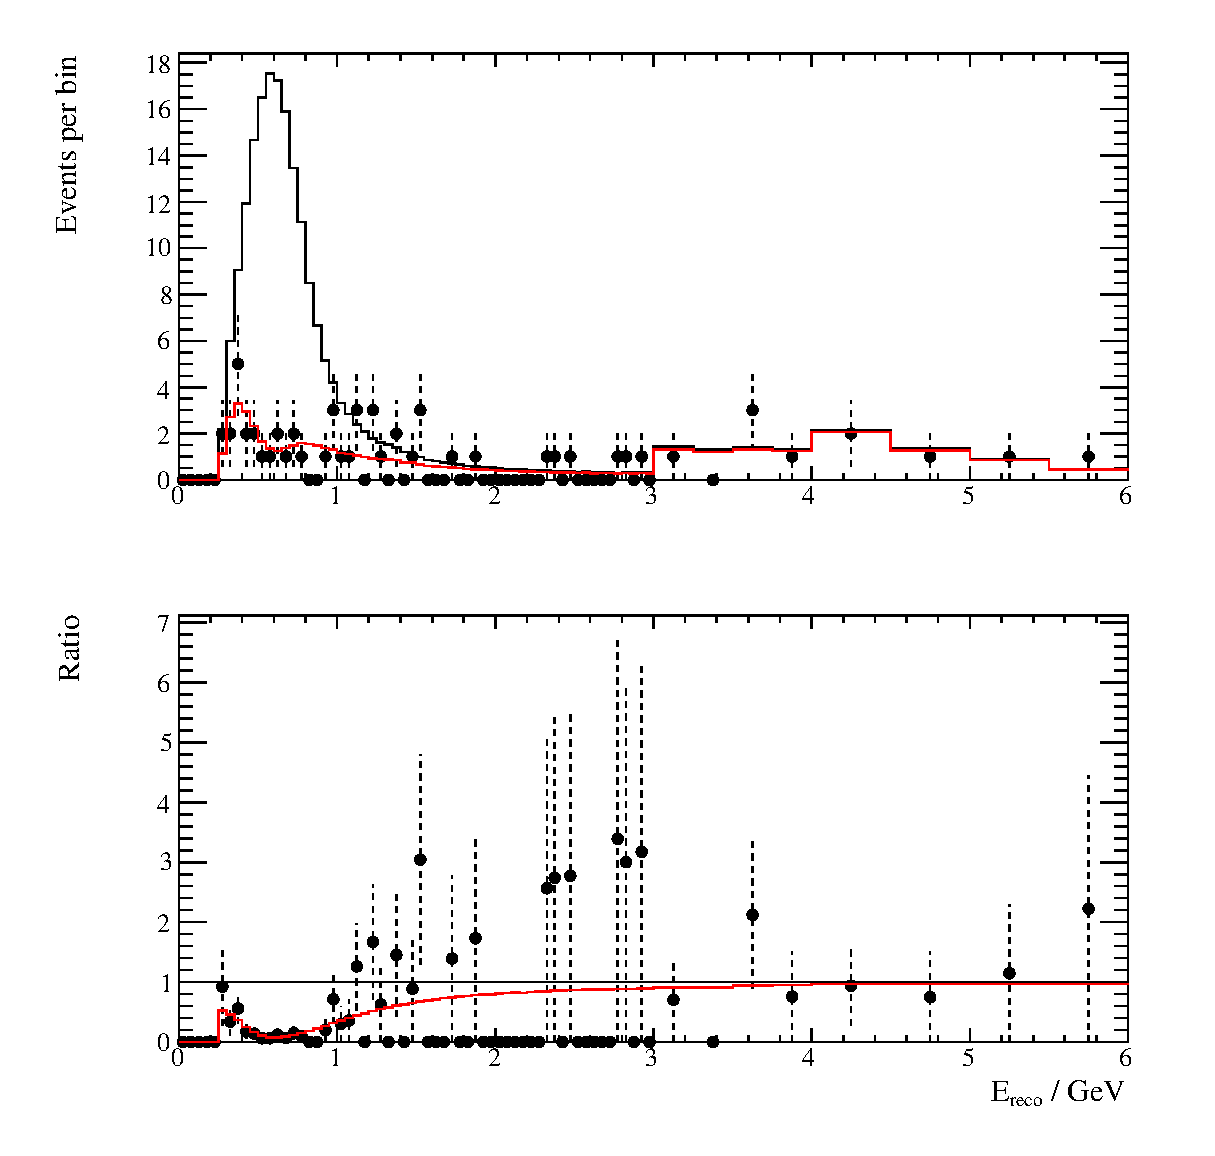
\includegraphics[width=28pc]{./images/fit_data/28/spectrum_3}
\caption {
  Best-fit reconstructed energy spectrum (top) obtained from the `2+8' fit to the combined Run 1+2+3 dataset.
  The Run 1+2+3 dataset and the prediction obtained from the no-oscillation hypothesis are also shown.
  The spectra are shown using the 73 bins used in the fit (see Sec.\ \ref{sec:mc_templates:template_binning}).
  The ratio of the data and best-fit distribution to the no-oscillation hypothesis is shown 
  in the bottom plot. The characteristic energy-dependent deficit can be clearly seen.
}
\label{fig:results_data123_spectrum}
\end{figure*}

\begin{figure*}[htb]
\begin{minipage}[t]{0.48\linewidth}
\center
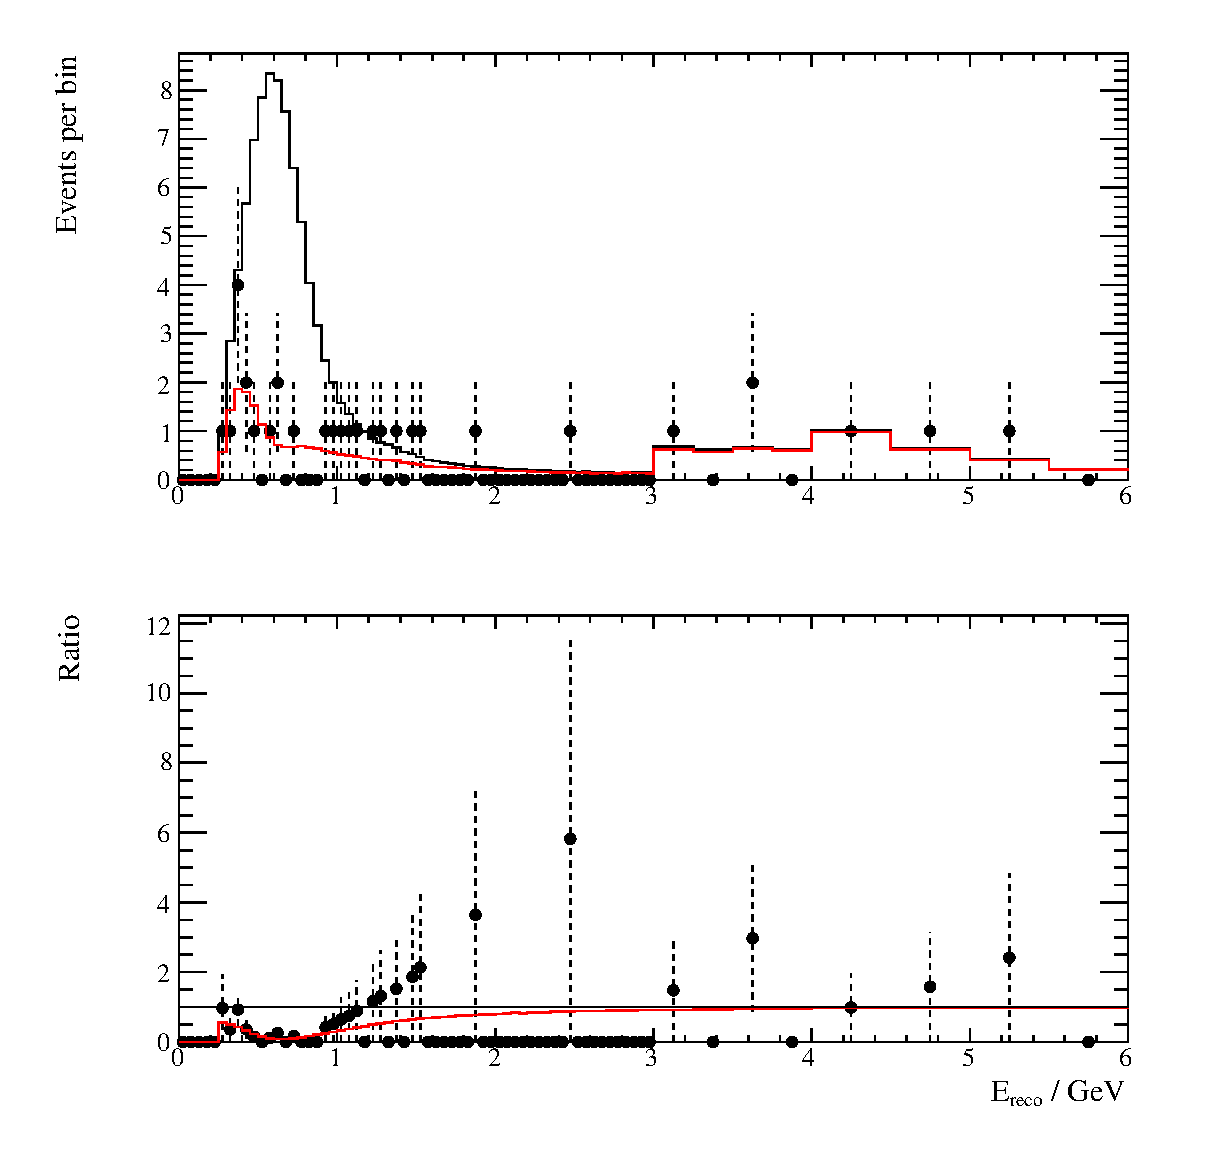
\includegraphics[width=20pc]{./images/fit_data/28/spectrum_4}
\caption {
  As in Fig.\ \ref{fig:results_data123_spectrum}, but for the Run 1+2 dataset only.
}
\label{fig:results_data12_spectrum}
\end{minipage}
\hspace{0.06\linewidth}
\begin{minipage}[t]{0.48\linewidth}
\center
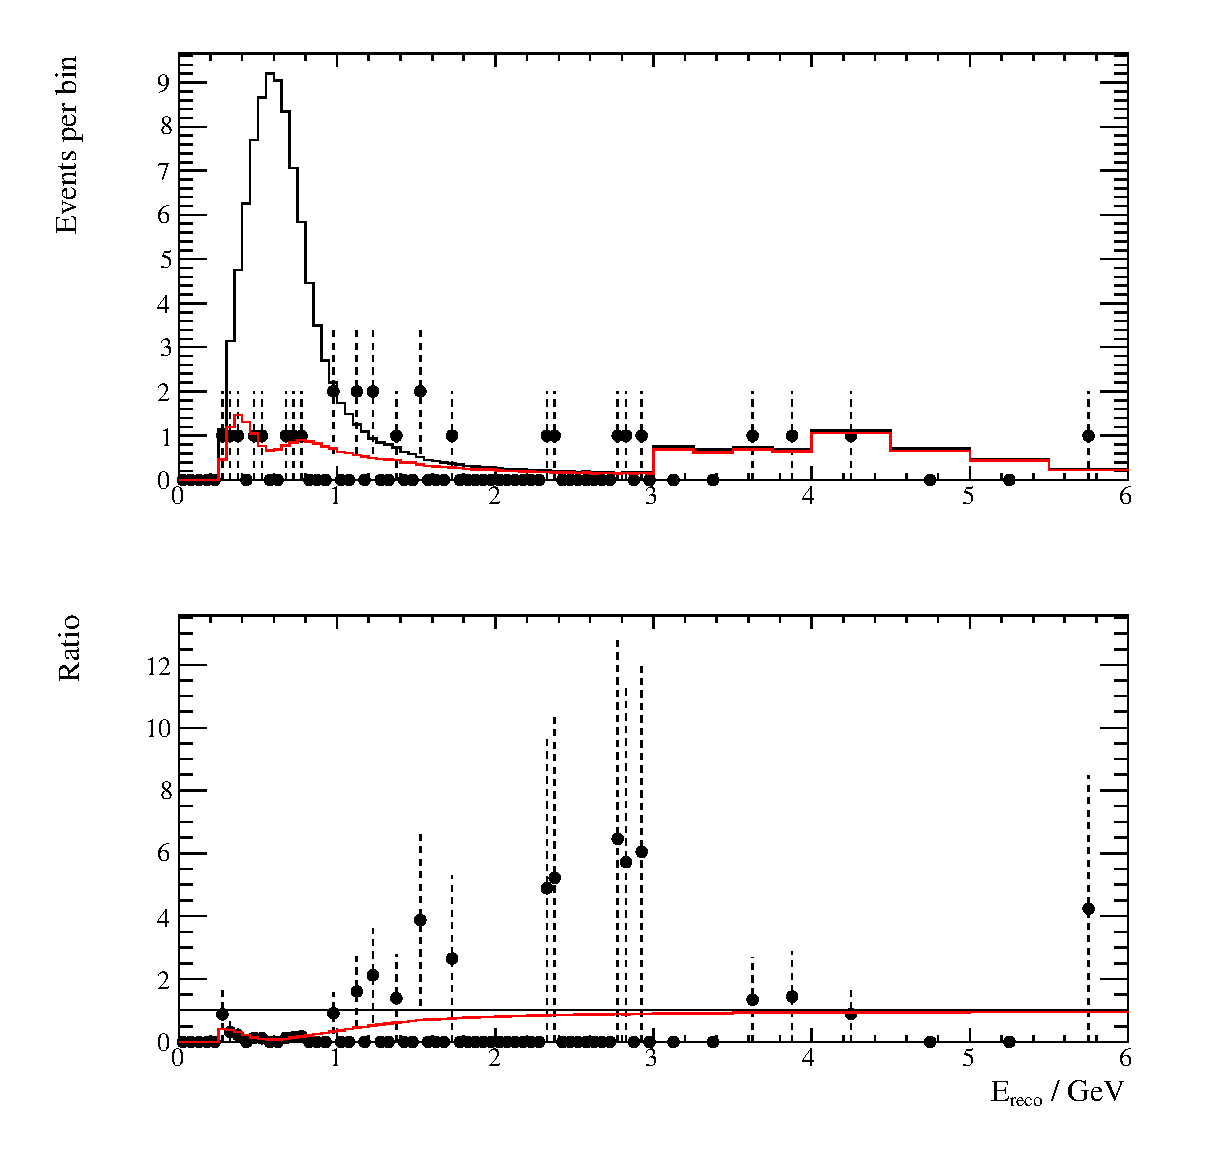
\includegraphics[width=20pc]{./images/fit_data/28/spectrum_5}
\caption {
  As in Fig.\ \ref{fig:results_data123_spectrum}, but for the Run 3 dataset only.
}
\label{fig:results_data3_spectrum}
\end{minipage}
\end{figure*}

%...........................................................
%
% Best-fit spectra (total and components) and ratios for `2+N' fit in sintheta
% (Run1+2+3 only, coarse binning)
%

\begin{figure*}[htb]
\center
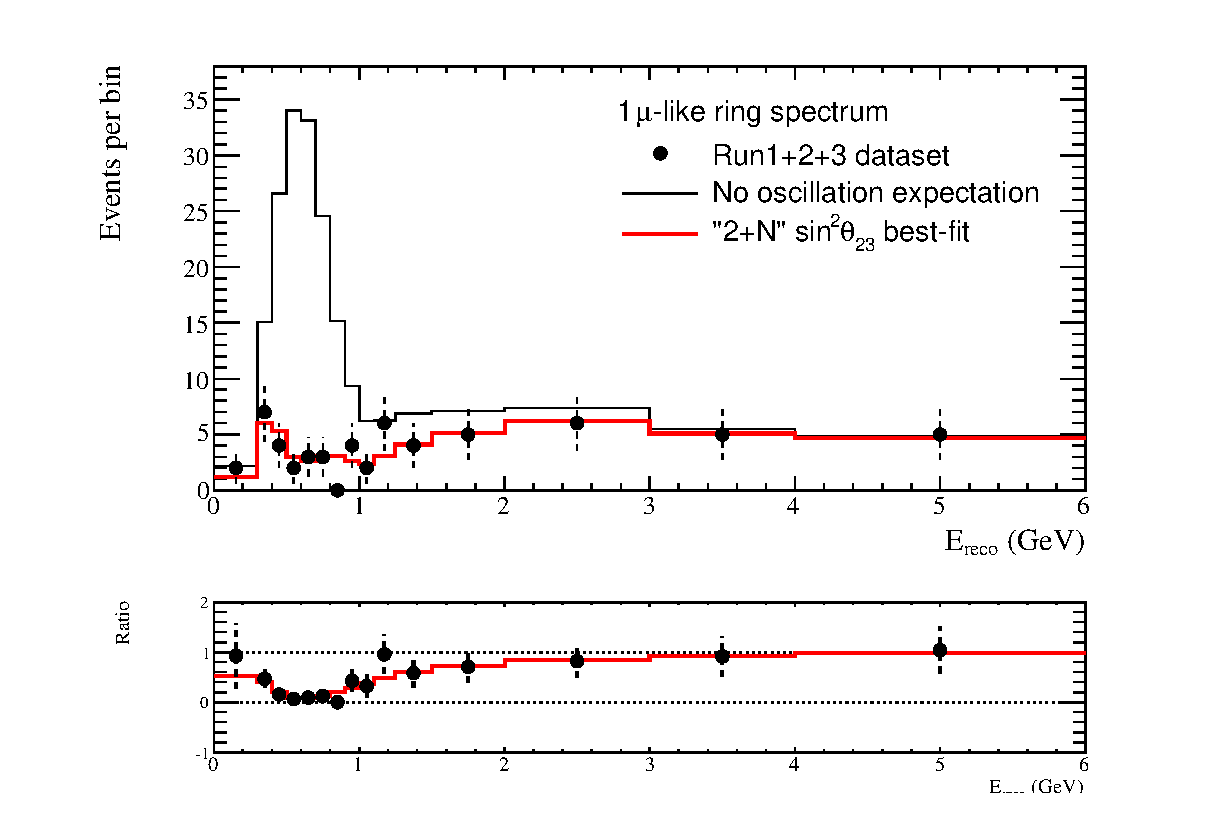
\includegraphics[width=34pc]{./images/fit_data/2Nsintheta/spectrum_and_ratio_2Nsintheta_coarse.eps}
\caption {
  Best-fit reconstructed energy spectrum using the coarse binning scheme (see 
  Sec.\ \ref{sec:results_bestfit_spectra}) obtained from the `2+N' $\sin^2\theta_{23}$ fit to the Run 1+2+3 dataset.
  Also shown are the spectrum obtained under the no-oscillation hypothesis
  and the ratios of the data and best-fit spectrum to it.
}
\label{fig:results_data123_spectrum_coarse_2Nsintheta}
\end{figure*}

\begin{figure*}[htb]
\center
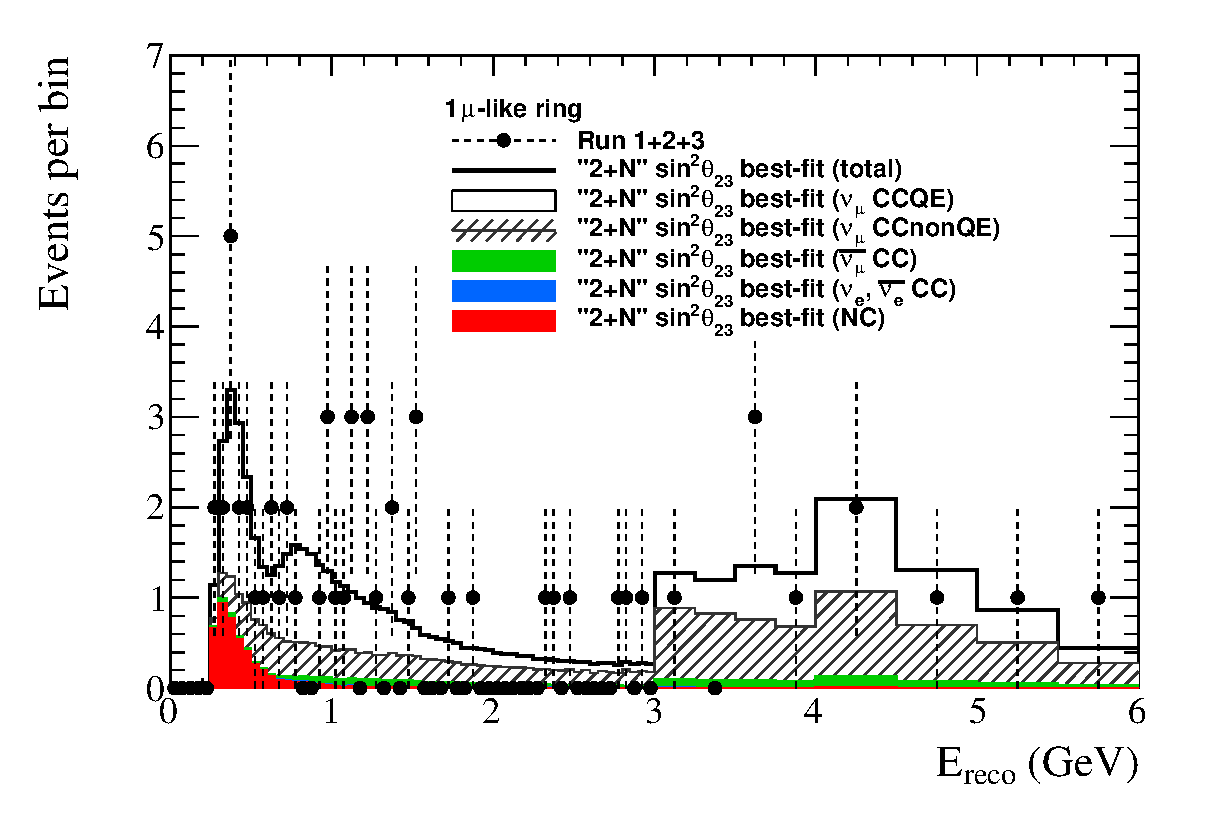
\includegraphics[width=24pc]{./images/fit_data/2Nsintheta/bestfit_spectrum_with_modes_run123_2Nsintheta.eps}
\caption {
  Best-fit reconstructed energy spectrum in the 73-bin scheme used in the fit (see 
  Sec.\ \ref{sec:mc_templates:template_binning}) and its components
  obtained from the `2+N' $\sin^2\theta_{23}$ fit to the Run 1+2+3 dataset.  
  The 28 components, each of which is calculated separately, are grouped into just 5 categories:
  $\nu_{\mu}$ CCQE, $\nu_{\mu}$ CCnQE, $\bar{\nu_{\mu}}$ CC, $\nu_{e}$/$\bar{\nu_{e}}$ CC and NC.  
}
\label{fig:results_data123_spectrum_components_2Nsintheta}
\end{figure*}


%...........................................................
%
% Best-fit spectra (total and components) and ratios for `2+N' fit 
% (Run1+2+3 only, coarse binning)
%

\begin{figure*}[htb]
\center
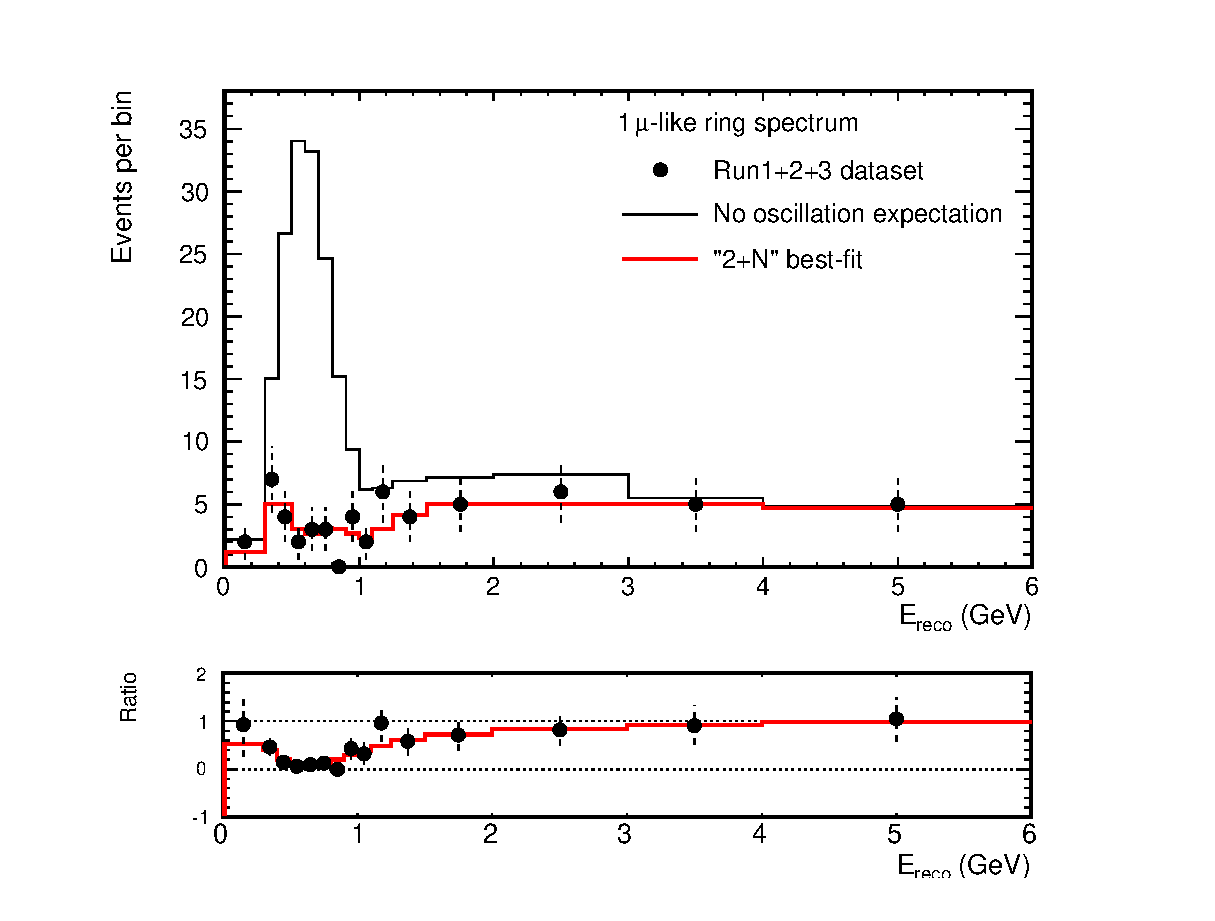
\includegraphics[width=34pc]{./images/fit_data/2N/spectrum_and_ratio_2N_coarse.eps}
\caption {
  Best-fit reconstructed energy spectrum using the coarse binning scheme (see 
  Sec.\ \ref{sec:results_bestfit_spectra}) obtained from the `2+N' fit to the Run 1+2+3 dataset.
  Also shown are the spectrum obtained under the no-oscillation hypothesis
  and the ratios of the data and best-fit spectrum to it.
}
\label{fig:results_data123_spectrum_coarse_2N}
\end{figure*}

\begin{figure*}[htb]
\center
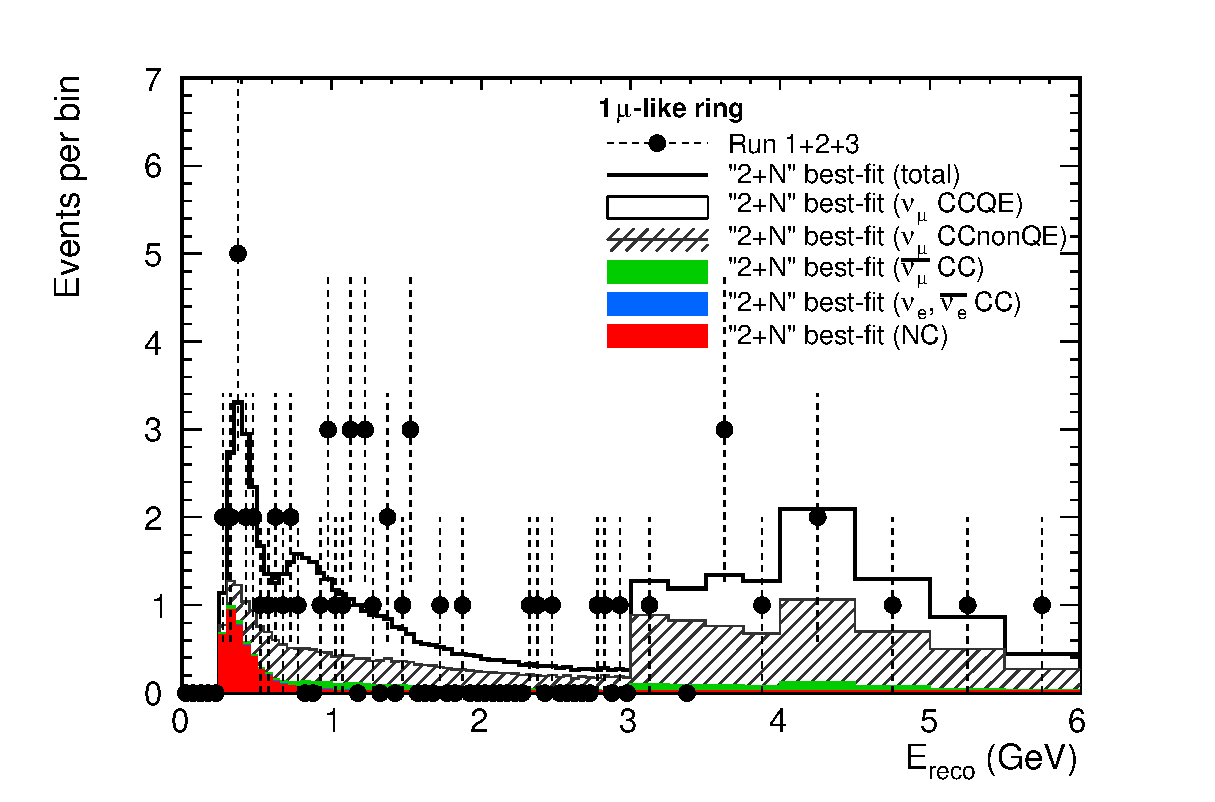
\includegraphics[width=24pc]{./images/fit_data/2N/bestfit_spectrum_with_modes_run123_2N.eps}
\caption {
  Best-fit reconstructed energy spectrum in the 73-bin scheme used in the fit (see 
  Sec.\ \ref{sec:mc_templates:template_binning}) and its components
  obtained from the `2+N' fit to the Run 1+2+3 dataset.  
  The 28 components, each of which is calculated separately, are grouped into just 5 categories:
  $\nu_{\mu}$ CCQE, $\nu_{\mu}$ CCnQE, $\bar{\nu_{\mu}}$ CC, $\nu_{e}$/$\bar{\nu_{e}}$ CC and NC.  
}
\label{fig:results_data123_spectrum_components_2N}
\end{figure*}

%...........................................................
%
% Best-fit spectra (total and components) and ratios for `2+N' fit in the second octant
% (Run1+2+3 only, coarse binning)
%

\begin{figure*}[htb]
\center
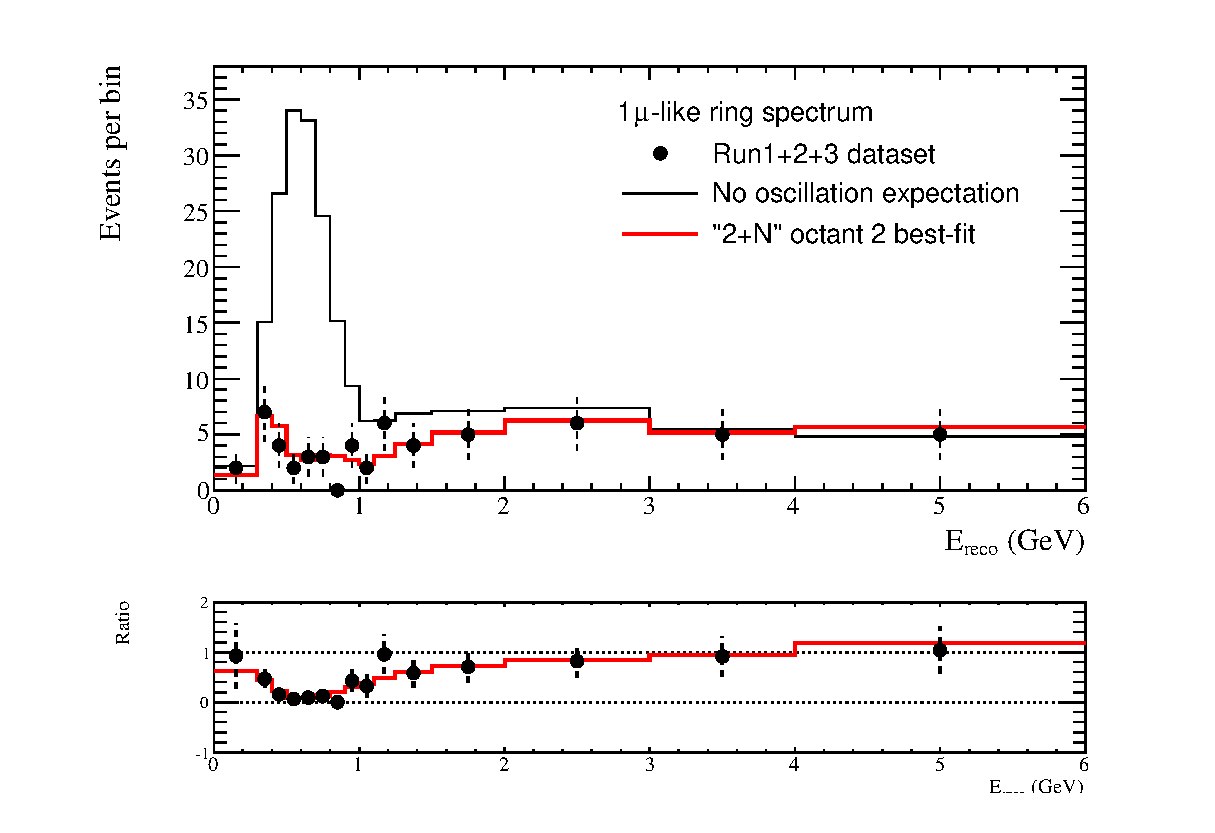
\includegraphics[width=34pc]{./images/fit_data/2Noctant2/spectrum_and_ratio_2N_coarse.eps}
\caption {
  Best-fit reconstructed energy spectrum using the coarse binning scheme (see 
  Sec.\ \ref{sec:results_bestfit_spectra}) obtained from the `2+N' fit to the Run 1+2+3 dataset,
  assuming $\theta_{23}$ is in the second octant.
  Also shown are the spectrum obtained under the no-oscillation hypothesis
  and the ratios of the data and best-fit spectrum to it.
}
\label{fig:results_data123_spectrum_coarse_2NO2}
\end{figure*}

\begin{figure*}[htb]
\center
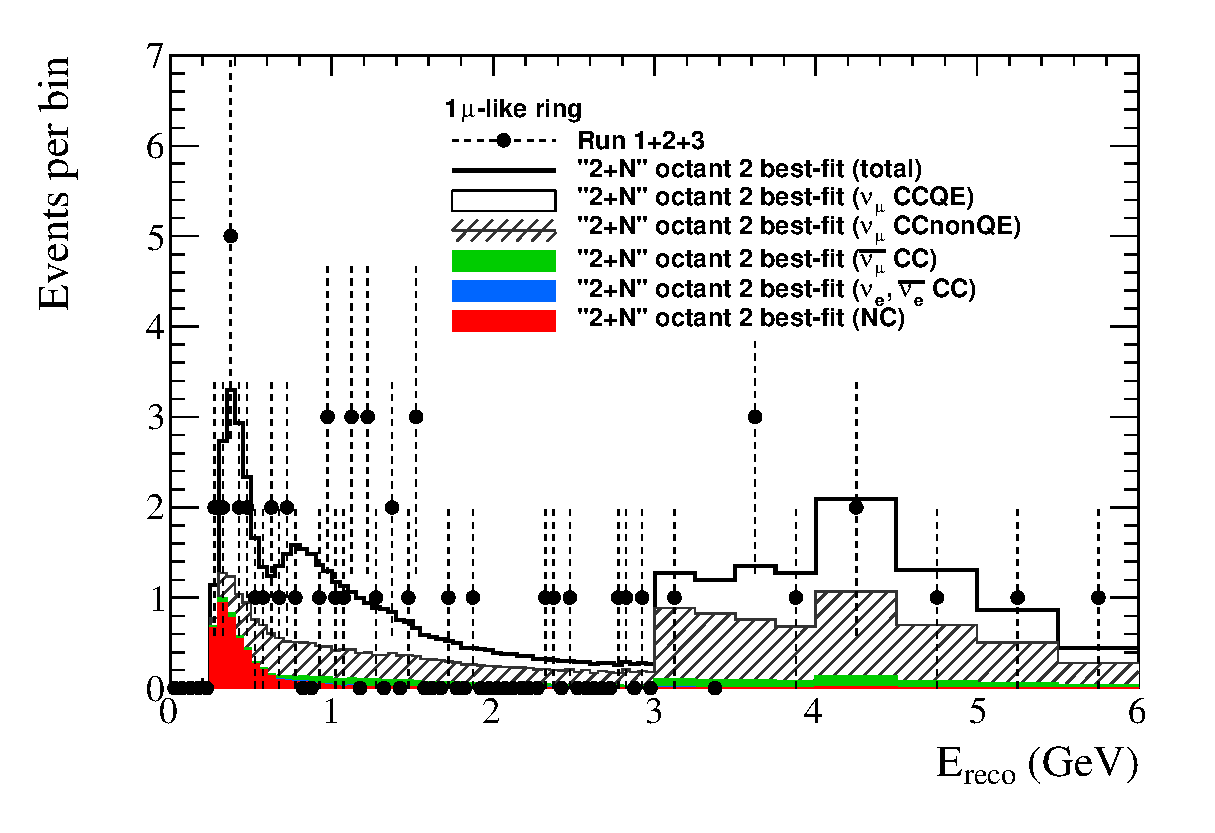
\includegraphics[width=24pc]{./images/fit_data/2Noctant2/bestfit_spectrum_with_modes_run123_2N.eps}
\caption {
  Best-fit reconstructed energy spectrum in the 73-bin scheme used in the fit (see 
  Sec.\ \ref{sec:mc_templates:template_binning}) and its components
  obtained from the `2+N' fit to the Run 1+2+3 dataset,
  assuming $\theta_{23}$ is in the the second octant.
  The 28 components, each of which is calculated separately, are grouped into just 5 categories:
  $\nu_{\mu}$ CCQE, $\nu_{\mu}$ CCnQE, $\bar{\nu_{\mu}}$ CC, $\nu_{e}$/$\bar{\nu_{e}}$ CC and NC.  
}
\label{fig:results_data123_spectrum_components_2NO2}
\end{figure*}

%...........................................................
%
% Best-fit spectra (total and components) and ratios for `2+8' fit 
% (Run1+2+3 only, coarse binning)
%

\begin{figure*}[htb]
\center
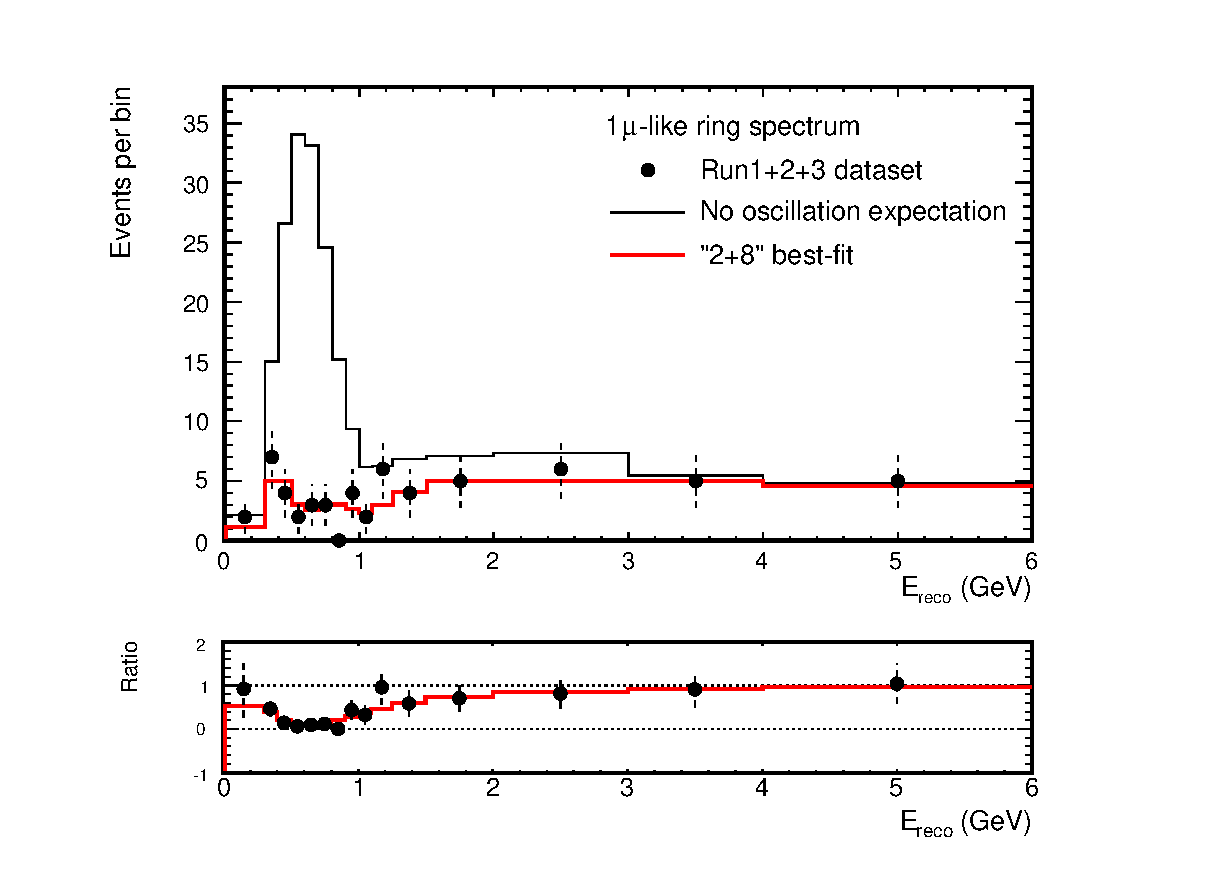
\includegraphics[width=34pc]{./images/fit_data/28/spectrum_and_ratio_28_coarse.eps}
\caption {
  Best-fit reconstructed energy spectrum using the coarse binning scheme (see 
  Sec.\ \ref{sec:results_bestfit_spectra})
  obtained from the `2+8' fit to the Run 1+2+3 dataset.
  Also shown are the spectrum obtained under the no-oscillation hypothesis
  and the ratios of the data and best-fit spectrum to it.
}
\label{fig:results_data123_spectrum_coarse}
\end{figure*}

\begin{figure*}[htb]
\center
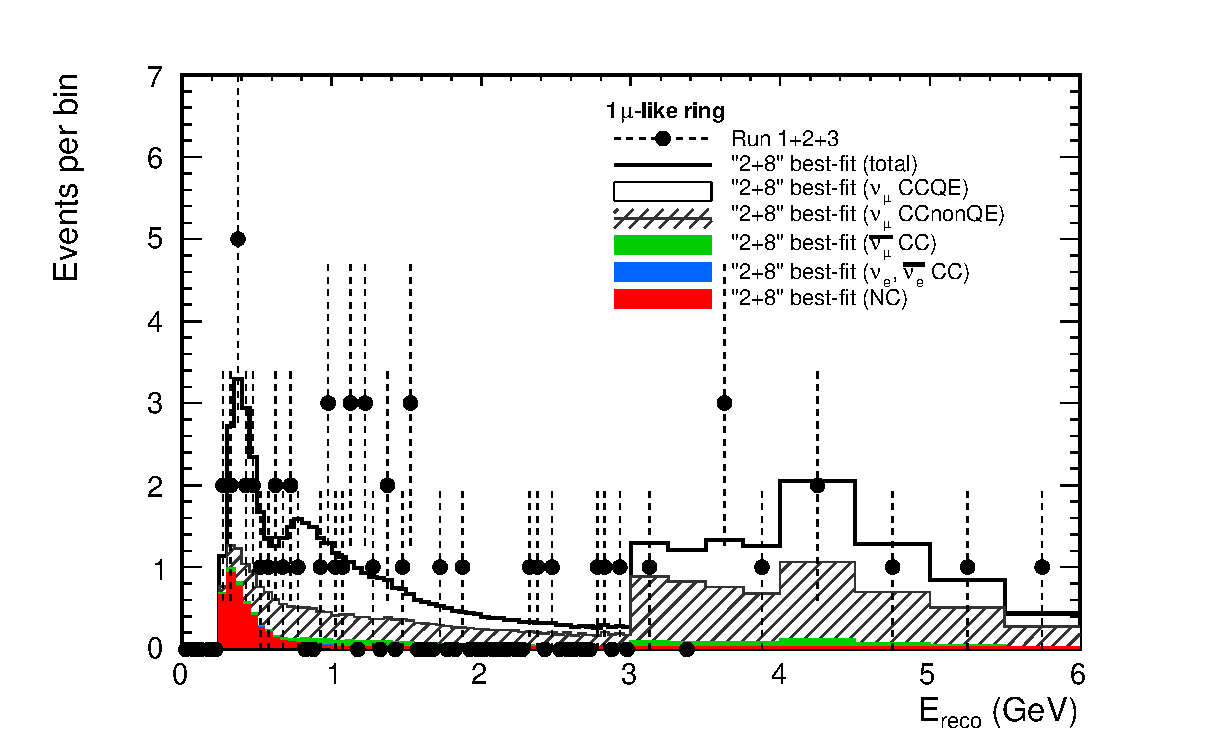
\includegraphics[width=24pc]{./images/fit_data/28/bestfit_spectrum_with_modes_run123_28.eps}
\caption {
  Best-fit reconstructed energy spectrum in the 73-bin scheme used in the fit (see
  Sec.\ \ref{sec:mc_templates:template_binning}) and its components
  obtained from the `2+8' fit to the Run 1+2+3 dataset.
  The 28 components, each of which is calculated separately, are grouped into just 5 categories:
  $\nu_{\mu}$ CCQE, $\nu_{\mu}$ CCnQE, $\bar{\nu_{\mu}}$ CC, $\nu_{e}$/$\bar{\nu_{e}}$ CC and NC.
}
\label{fig:results_data123_spectrum_components}
\end{figure*}

\clearpage
%...........................................................
%
% Comparison of `2+N' sintheta & second octant best-fit spectra and difference
% (Run1+2+3 only, 73 bins)
%

\begin{figure*}[htb]
\center
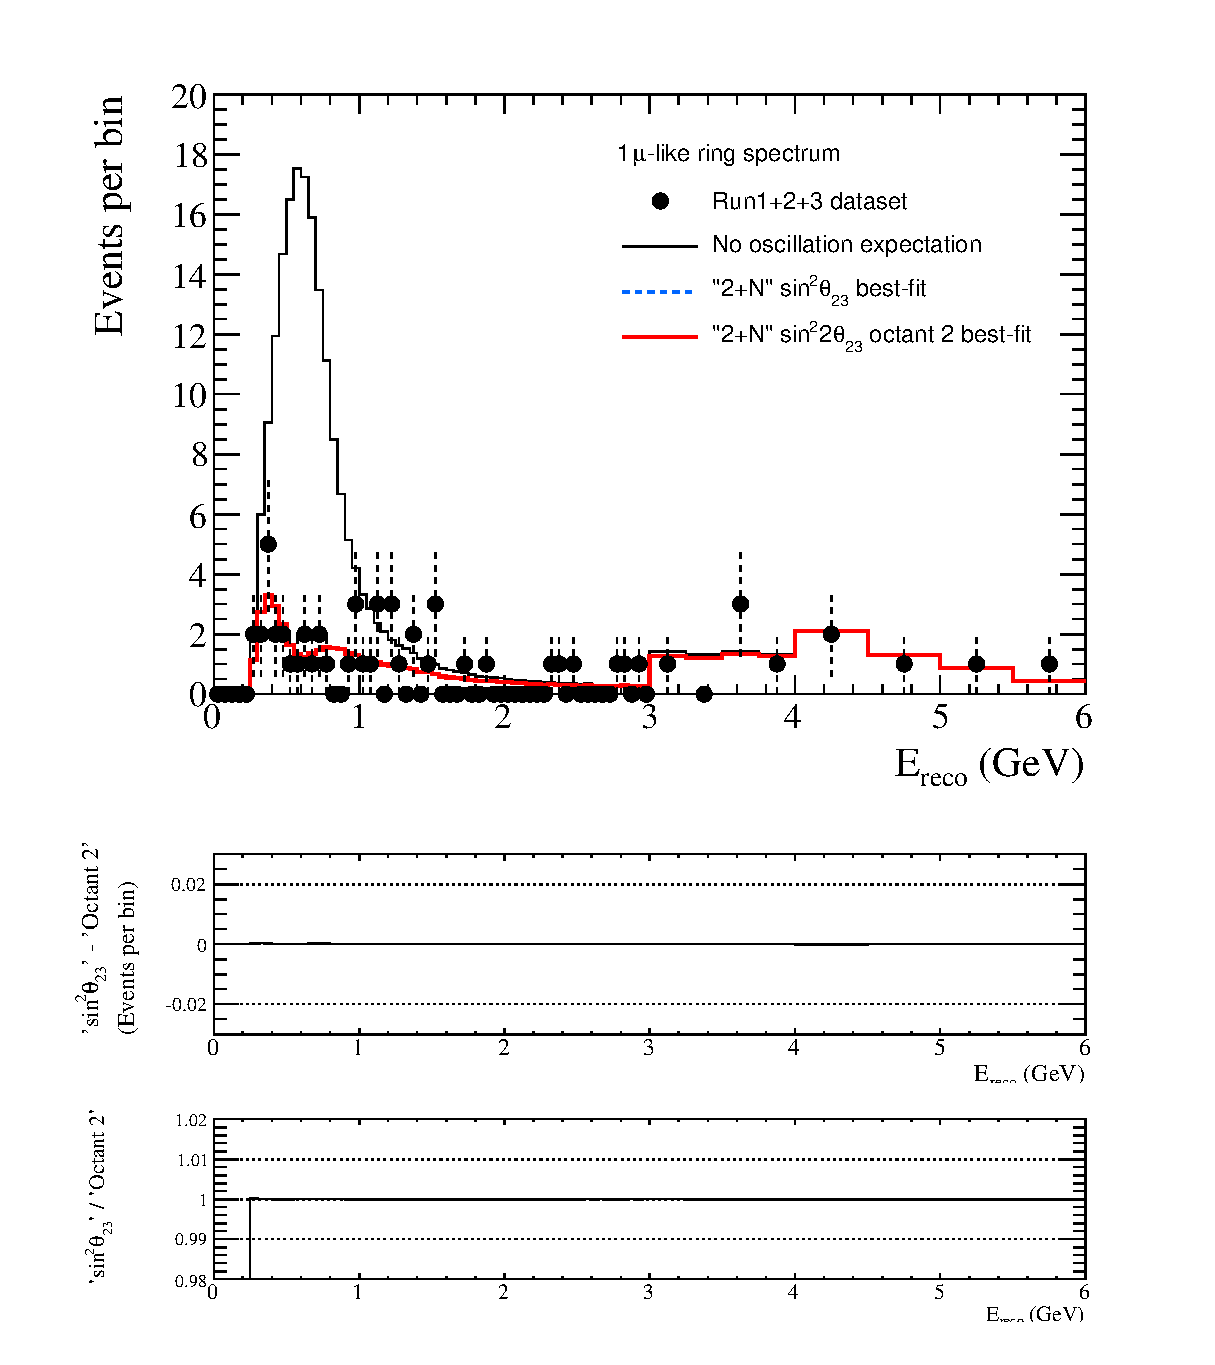
\includegraphics[width=40pc]{./images/fit_data/compare/spectrum_comparison_2Nsintheta_2NO2}
\caption {
  Comparison between best-fit reconstructed energy spectra
  obtained from the `2+N' fits to the Run 1+2+3 datasets, for
  the $\sin^2\theta_{23}$ fit, and the $\sin^2(2\theta_{23})$ fit assuming the second octant.
  The spectra are shown using the 73 bins used in the fit (see Sec.\ \ref{sec:mc_templates:template_binning}).
  Also shown are the absolute difference between the '$\sin^2\theta_{23}$' and '$\sin^2(2\theta_{23})$ octant 2' best-fit spectra and 
  the ratio between them.
}
\label{fig:results_data123_spectrum_comparison_sintheta}
\end{figure*}

%...........................................................
%
% Comparison of `2+N' sintheta & second octant best-fit spectra and fractional difference
% (Run1+2+3 only, coarser binning)
%

\begin{figure*}[htb]
\center
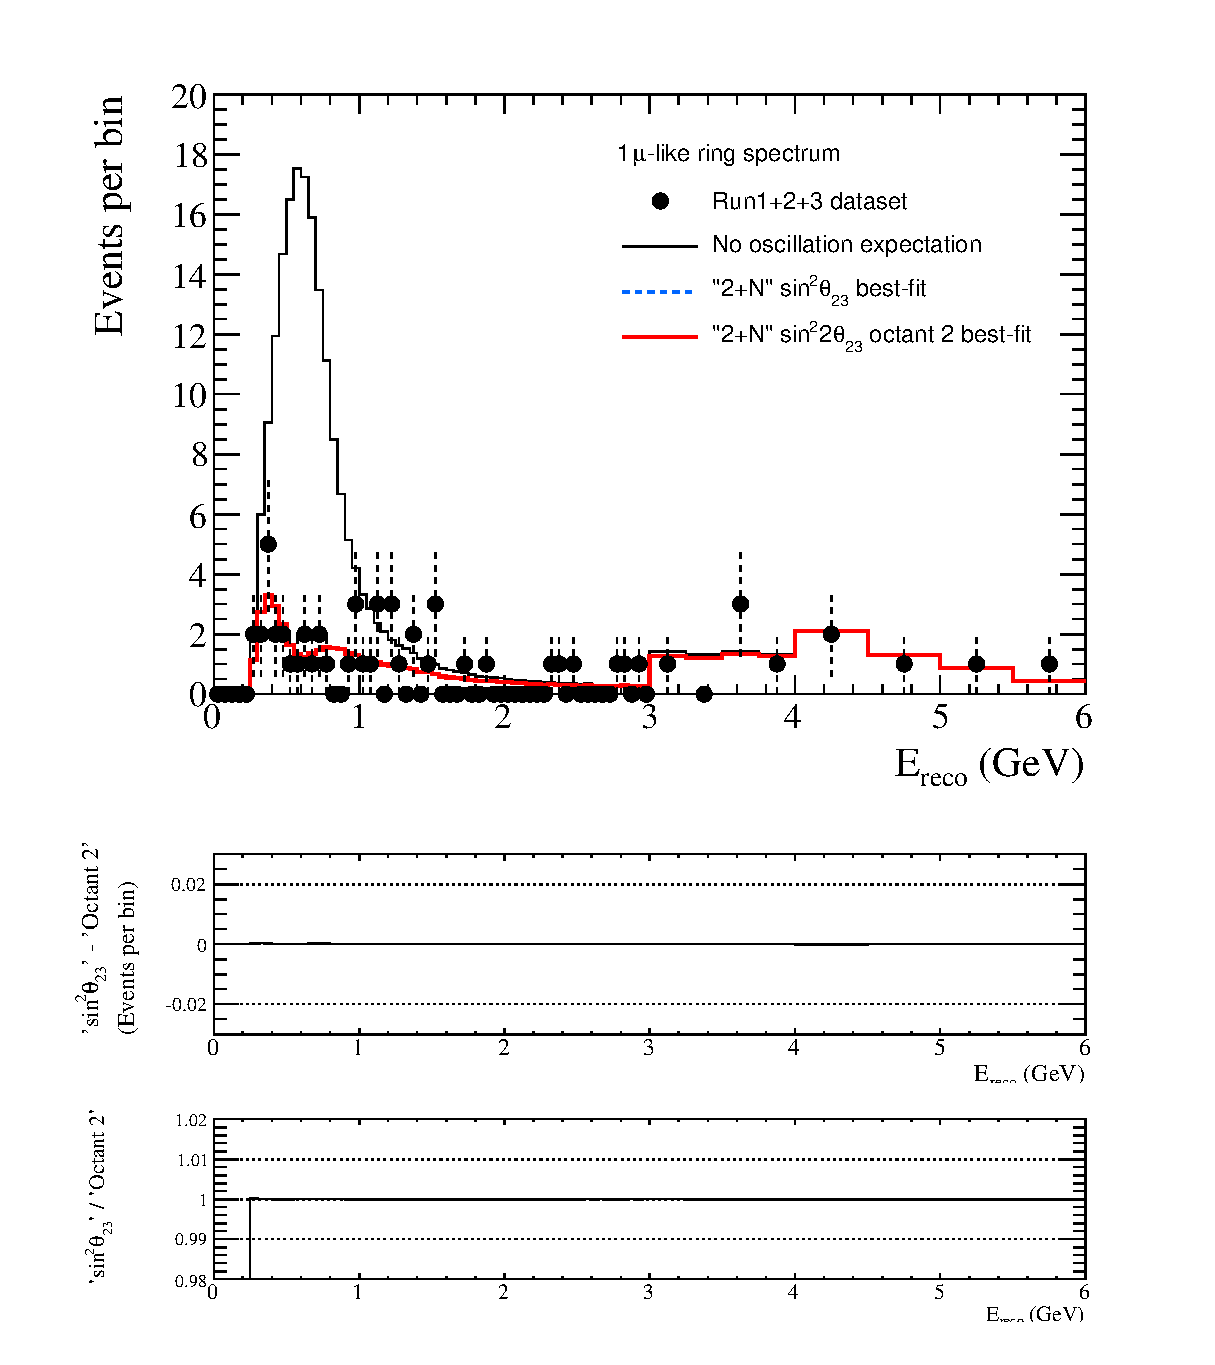
\includegraphics[width=40pc]{./images/fit_data/compare/spectrum_comparison_2Nsintheta_2NO2_coarse.eps}
\caption {
  Comparison between best-fit reconstructed energy spectra
  obtained from the `2+N' fits to the Run 1+2+3 datasets, for
  the $\sin^2\theta_{23}$ fit, and the $\sin^2(2\theta_{23})$ fit assuming the second octant.
  scheme (see Sec.\ \ref{sec:results_bestfit_spectra}).
  Also shown are the absolute difference between the '$\sin^2\theta_{23}$' and '$\sin^2(2\theta_{23})$ octant 2' best-fit spectra and 
  the ratio between them.
}
\label{fig:results_data123_spectrum_comparison_sintheta_coarse}
\end{figure*}


%...........................................................
%
% Comparison of `2+N' first & second octant best-fit spectra and difference
% (Run1+2+3 only, 73 bins)
%

\begin{figure*}[htb]
\center
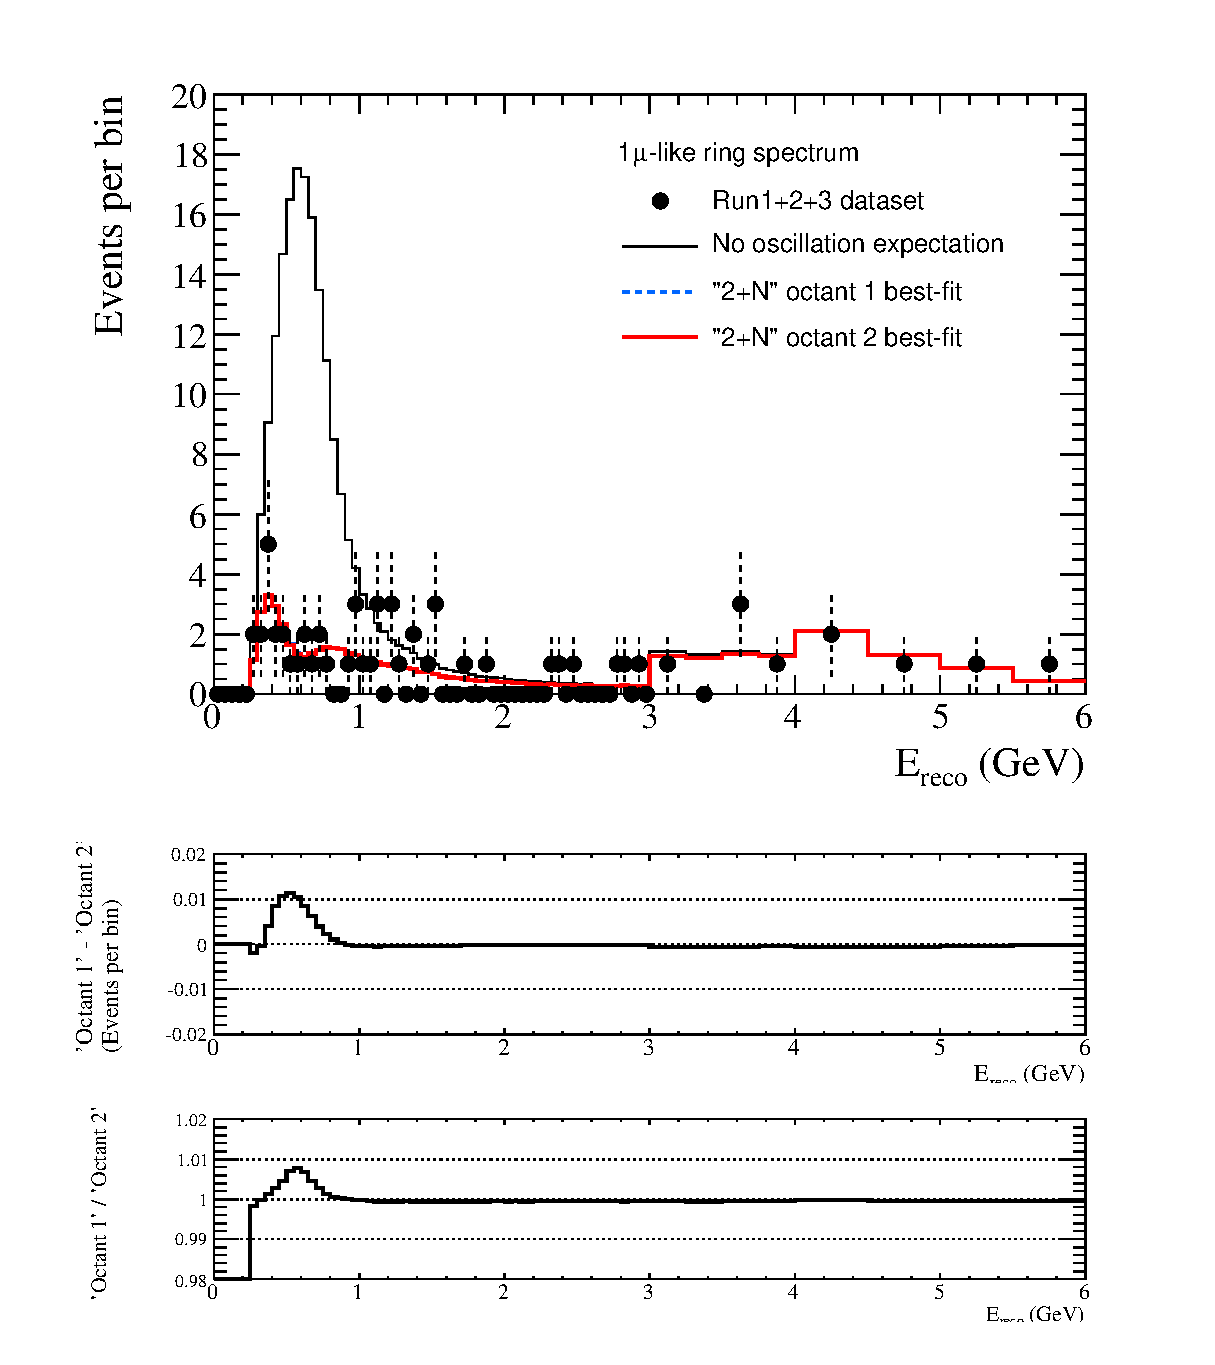
\includegraphics[width=40pc]{./images/fit_data/compare/spectrum_comparison_2N_2NO2}
\caption {
  Comparison between best-fit reconstructed energy spectra
  obtained from the `2+N' fits to the Run 1+2+3 datasets, for both $\theta_{23}$ octant assumptions.
  The spectra are shown using the 73 bins used in the fit (see Sec.\ \ref{sec:mc_templates:template_binning}).
  Also shown are the absolute difference between the '$\theta_{23}$ octant 1' and '$\theta_{23}$ octant 2' best-fit spectra and 
  the ratio between them.
}
\label{fig:results_data123_spectrum_comparison_octant}
\end{figure*}

%...........................................................
%
% Comparison of `2+N' first & second octant best-fit spectra and fractional difference
% (Run1+2+3 only, coarser binning)
%

\begin{figure*}[htb]
\center
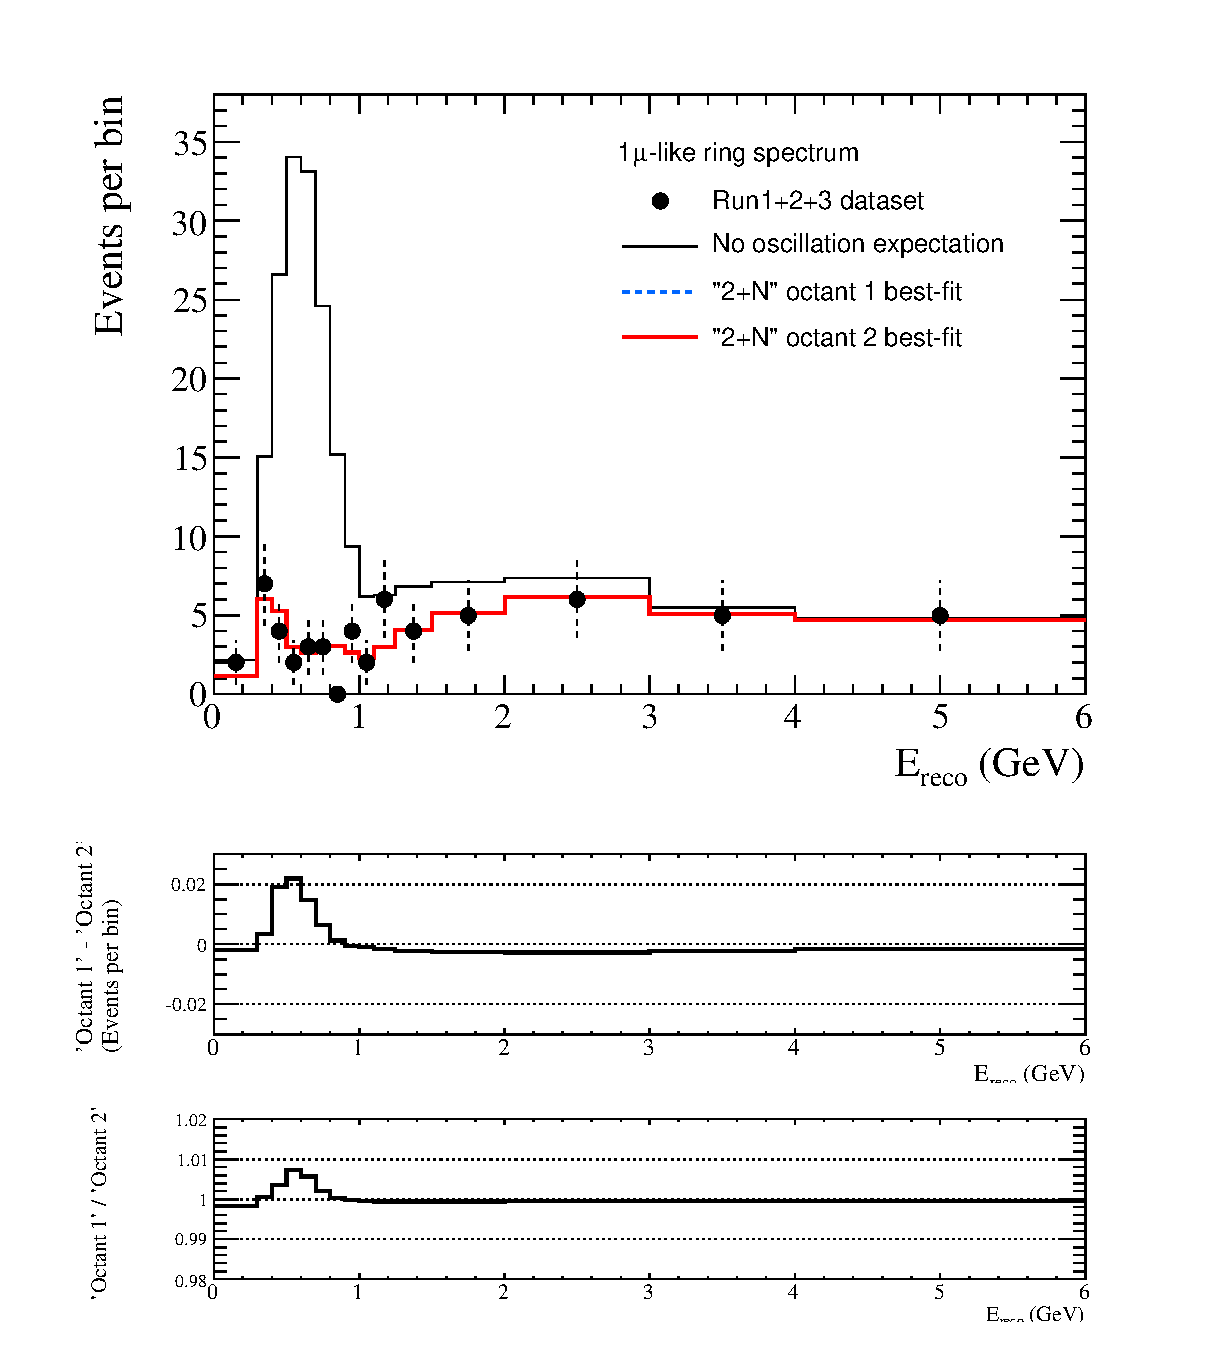
\includegraphics[width=40pc]{./images/fit_data/compare/spectrum_comparison_2N_2NO2_coarse.eps}
\caption {
  Comparison between best-fit reconstructed energy spectra
  obtained from the `2+N' fits to the Run 1+2+3 datasets, for both $\theta_{23}$ octant assumptions,
  using the coarse binning 
  scheme (see Sec.\ \ref{sec:results_bestfit_spectra}).
  Also shown are the absolute difference between the '$\theta_{23}$ octant 1' and '$\theta_{23}$ octant 2' best-fit spectra and
  the ratio between them.
}
\label{fig:results_data123_spectrum_comparison_octant_coarse}
\end{figure*}


%...........................................................
%
% Comparison of `2+N' and `2+8' best-fit spectra and difference
% (Run1+2+3 only, 73 bins)
%

\begin{figure*}[htb]
\center
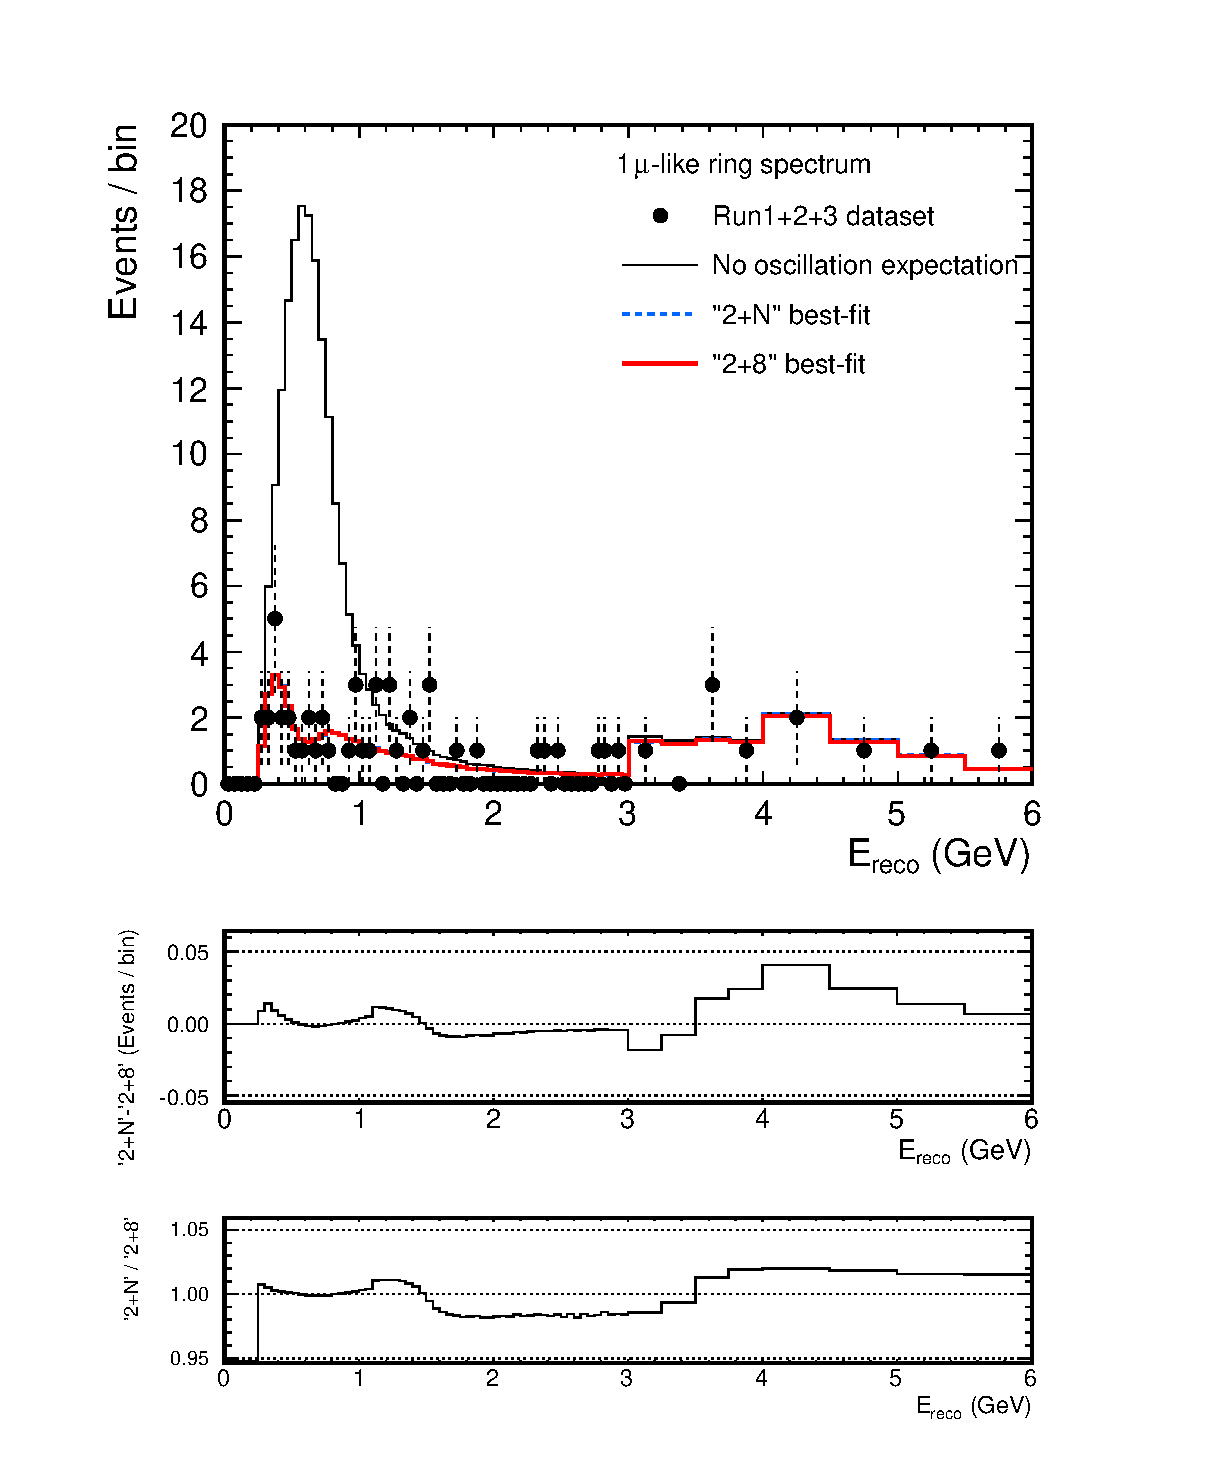
\includegraphics[width=40pc]{./images/fit_data/compare/spectrum_comparison_28_2N.eps}
\caption {
  Comparison between best-fit reconstructed energy spectra
  obtained from the `2+N' and `2+8' fits to the Run 1+2+3 datasets.
  The spectra are shown using the 73 bins used in the fit (see Sec.\ \ref{sec:mc_templates:template_binning}).
  Also shown are the absolute difference between the '2+N' and '2+8' best-fit spectra and 
  the ratio between them.
}
\label{fig:results_data123_spectrum_comparison}
\end{figure*}

%...........................................................
%
% Comparison of `2+N' and `2+8' best-fit spectra and fractional difference
% (Run1+2+3 only, coarser binning)
%

\begin{figure*}[htb]
\center
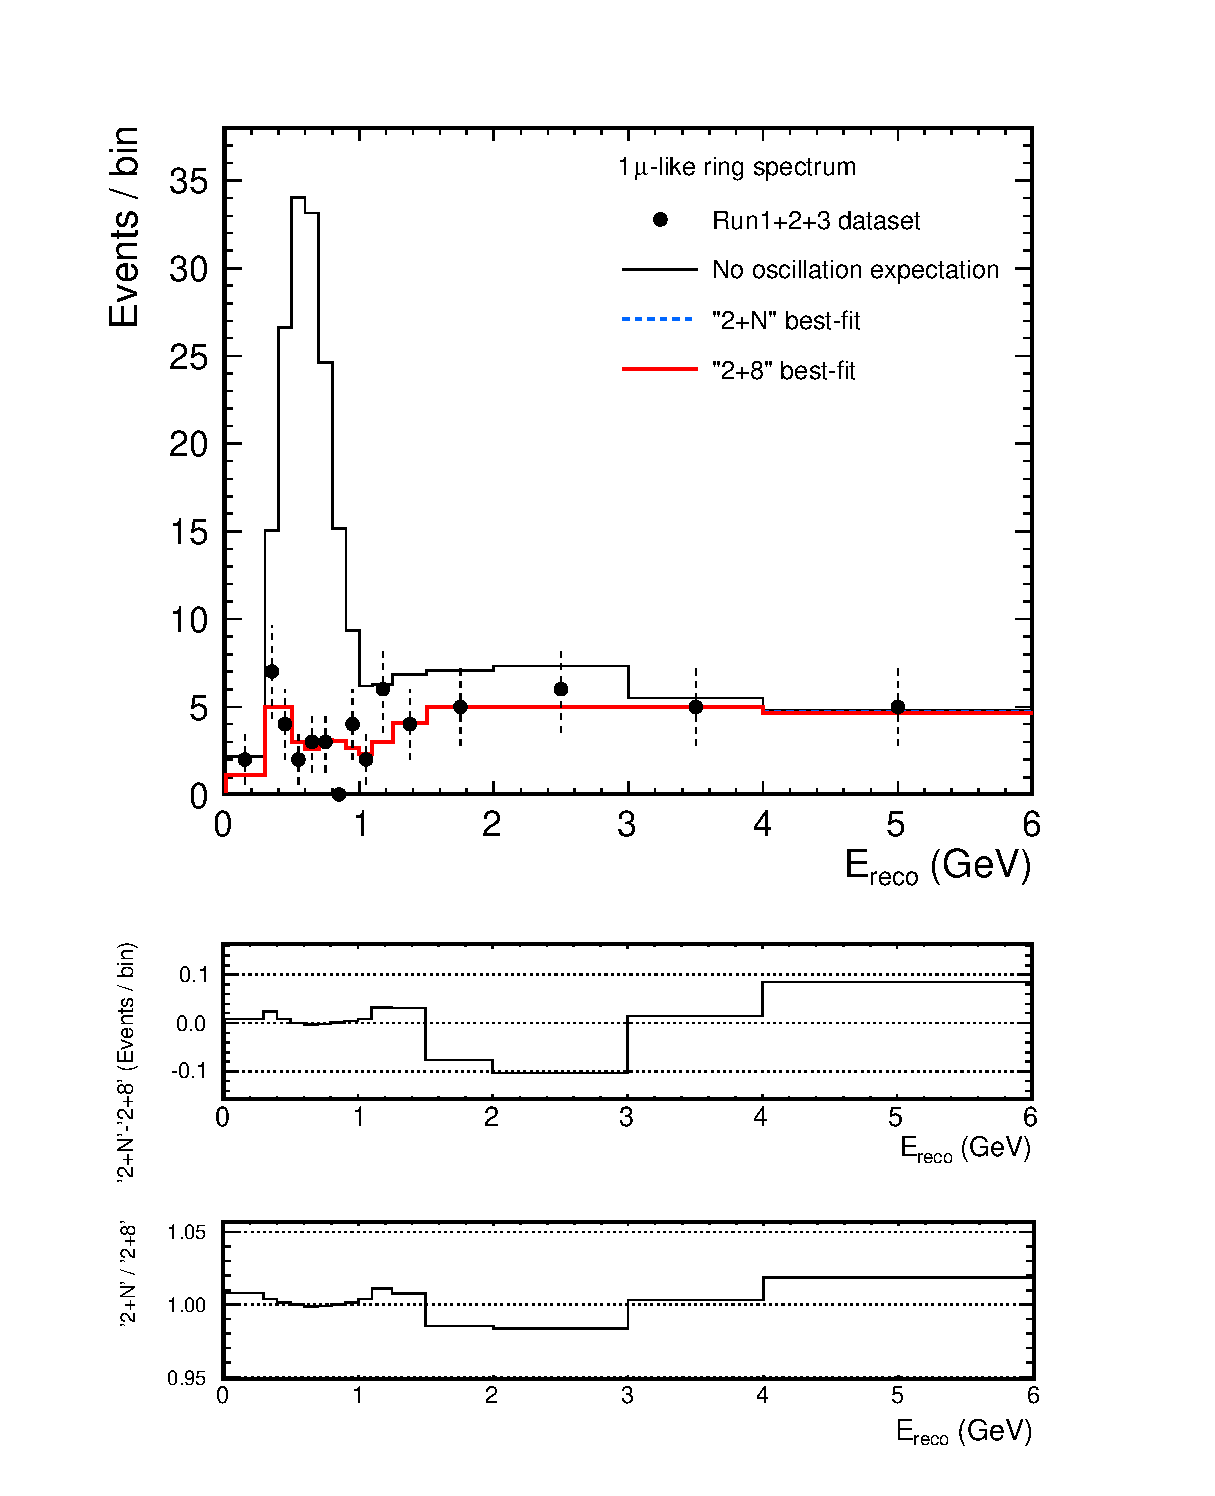
\includegraphics[width=40pc]{./images/fit_data/compare/spectrum_comparison_28_2N_coarse.eps}
\caption {
  Comparison between best-fit reconstructed energy spectra
  obtained from the `2+N' and `2+8' fits to the Run 1+2+3 datasets using the coarse binning 
  scheme (see Sec.\ \ref{sec:results_bestfit_spectra}).
  Also shown are the absolute difference between the '2+N' and '2+8' best-fit spectra and
  the ratio between them.
}
\label{fig:results_data123_spectrum_comparison_coarse}
\end{figure*}


%--------------------------------------------------------------------------------------
% Limits
%--------------------------------------------------------------------------------------

\clearpage

\subsection {Confidence limits}
\label{sec:results_limits}

The first step in calculating confidence limits for a single oscillation
parameter is to calculate the values of $\Delta\chi^2$ for each value of that oscillation 
parameter. For each value of $\sin^{2}2\theta_{23}$, a `1+N' fit is done with $|\Delta m^{2}_{32}|$ 
and all the systematic parameters allowed to float and $\sin^{2}2\theta_{23}$ fixed. Then 
$\Delta\chi^2$ is calculated for that value of $\sin^{2}2\theta_{23}$ by subtracting 
the `2+N' best-fit value of $\chi^2$ over the whole 2D oscillation parameter grid 
(which is listed in Tab.\ \ref{tab:data_fits:best_fit_values}). The 68\% and 90\% 
confidence intervals in $\sin^{2}2\theta_{23}$ are found using the constant-$\Delta\chi^2$ method, 
as described in Sec.\ \ref{sec:contour_construction_constdchi}, and are given by the values for 
which $\chi^2$ increases from the minimum by 1.00 and 2.71 respectively. Then this procedure 
is repeated for $|\Delta m^{2}_{32}|$\footnote{
  The procedure is equivalent for the limits with $\sin^2\theta_{23}$,
  just with a different fit parameter.
}.

The constant-$\Delta \chi^{2}$ method is used for the 1D confidence
limits since there is a problem in using the Feldman-Cousins
method. There is no obvious way of choosing the true value(s) of
$|\Delta m_{32}^{2}|$ as inputs to the toy MC experiments to find the
critical values of $\Delta \chi^{2}$ for the 1D confidence interval in
$\sin^{2} 2\theta_{23}$. The same difficulty arises when choosing the
true values of $\sin^{2} 2\theta_{23}$ to find the critical values of
$\Delta \chi^{2}$ for the 1D confidence interval in $|\Delta
m_{32}^{2}|$.

The $\Delta\chi^2$ distributions for $\sin^{2}\theta_{23}$ and $|\Delta m^{2}_{32}|$ for the 
`1+N' fit to the Run 1+2+3 dataset are shown in Figs.\
\ref{fig:results_data123_1dcontour_mixing23_sintheta} and
\ref{fig:results_data123_1dcontour_dm23sq_sintheta} respectively, along with the
68\% and 90\% constant-$\Delta\chi^2$ critical values.
These provide the 68\% errors $\sin^{2}\theta_{23} = 0.514\pm0.082$
and $|\Delta m^2_{32}| = 2.44^{+0.17}_{-0.15}$$\times$10$^{-3}$ eV$^{2}$/c$^{4}$,
and the limits of
$0.397 < \sin^{2}\theta_{23} < 0.630$
and
$2.19$$\times$10$^{-3}$ eV$^{2}$/c$^{4}$ $< |\Delta m^2_{32}| < 2.72$$\times$10$^{-3}$ eV$^{2}$/c$^{4}$
at 90\% C.L.

The $\Delta\chi^2$ distributions for $\sin^{2}2\theta_{23}$ and $|\Delta m^{2}_{32}|$ for the 
`1+N' fit to the Run 1+2+3 dataset are shown in Figs.\
\ref{fig:results_data123_1dcontour_mixing23} and
\ref{fig:results_data123_1dcontour_dm23sq} respectively, along with the
68\% and 90\% constant-$\Delta\chi^2$ critical values.
Results are shown for $\theta_{23}$ in both the first and second octants.
For the first octant, these provide the 68\% errors $\sin^{2}2\theta_{23} = 1.000^{+0.000}_{-0.019}$
and $|\Delta m^2_{32}| = 2.44^{+0.17}_{-0.15}$$\times$10$^{-3}$ eV$^{2}$/c$^{4}$,
and the limits of $\sin^{2}2\theta_{23}$ $>$ 0.958 and
$2.19$$\times$10$^{-3}$ eV$^{2}$/c$^{4}$ $< |\Delta m^2_{32}| < 2.72$$\times$10$^{-3}$ eV$^{2}$/c$^{4}$
at 90\% C.L. 
For the second octant, these provide the 68\% errors $\sin^{2}2\theta_{23} = 0.999^{+0.001}_{-0.036}$
and $|\Delta m^2_{32}| = 2.44^{+0.17}_{-0.15}$$\times$10$^{-3}$ eV$^{2}$/c$^{4}$,
and the limits of $\sin^{2}2\theta_{23}$ $>$ 0.931 and
$2.19$$\times$10$^{-3}$ eV$^{2}$/c$^{4}$ $< |\Delta m^2_{32}| < 2.72$$\times$10$^{-3}$ eV$^{2}$/c$^{4}$
at 90\% C.L.
The 1D limits for the second octant are identical to those for the first octant for $|\Delta m^2_{32}|$,
but much wider for $\sin^{2}2\theta_{23}$.
This can be understood from Eq.\ \ref{eqn:numusurv3fapprox} since
the center of symmetry (point of maximal disappearance) is in the second octant.

%...........................................................
%
% sinsqtheta23 fit limits
%

\begin{figure*}[htb]
%\begin{minipage}[t]{0.90\linewidth}
\begin{minipage}[t]{0.48\linewidth}
\center
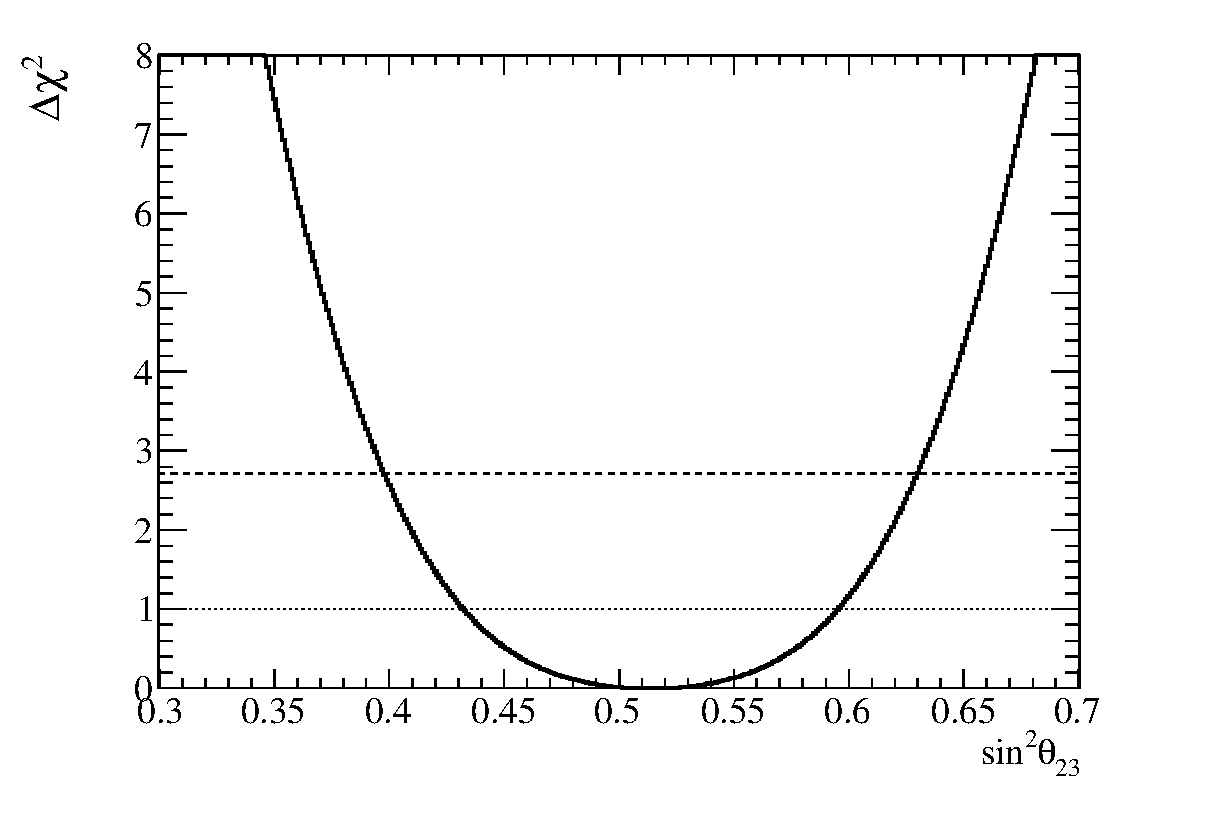
\includegraphics[width=20pc]{./images/fit_data/2Nsintheta/1D_contour_mixing23_lines}
\caption {$\Delta \chi^2$ as a function of $\sin^2\theta_{23}$
  for the `1+N' fit to the Run 1+2+3 dataset.
  The 68\% and 90\% constant-$\Delta\chi^2$ critical values are shown
  as dotted and dashed lines respectively.
}
\label{fig:results_data123_1dcontour_mixing23_sintheta}
\end{minipage}
%\vfill
\hspace{0.06\linewidth}
%\begin{minipage}[t]{0.90\linewidth}
\begin{minipage}[t]{0.48\linewidth}
\center
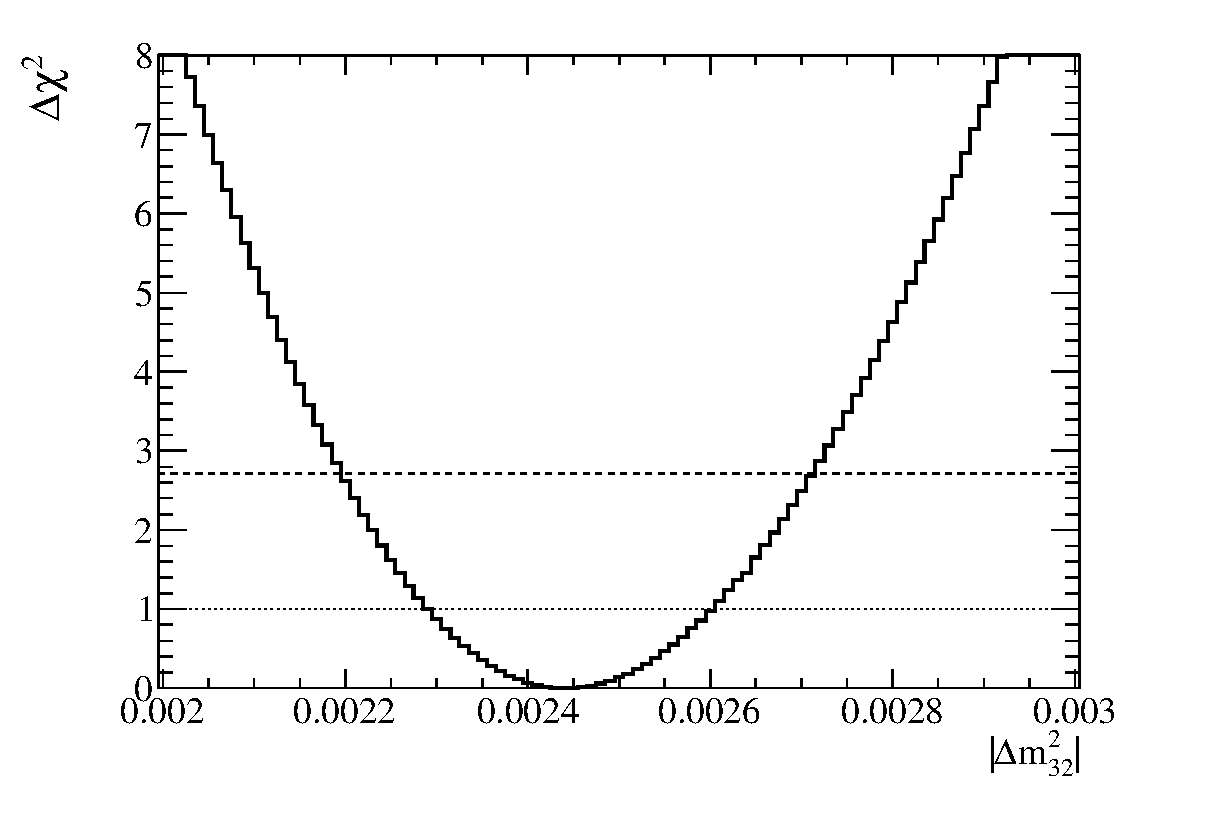
\includegraphics[width=20pc]{./images/fit_data/2Nsintheta/1D_contour_dm23sq_lines}
\caption { 
  $\Delta \chi^2$ as a function of $|\Delta m^{2}_{32}|$
  for the `1+N' fit to the Run 1+2+3 dataset.
  The 68\% and 90\% constant-$\Delta\chi^2$ critical values are shown
  as dotted and dashed lines respectively.
}
\label{fig:results_data123_1dcontour_dm23sq_sintheta}
\end{minipage}
\end{figure*}

%...........................................................
%
% sinsq2theta23 fit limits
%

\begin{figure*}[htb]
%\begin{minipage}[t]{0.90\linewidth}
\begin{minipage}[t]{0.48\linewidth}
\center
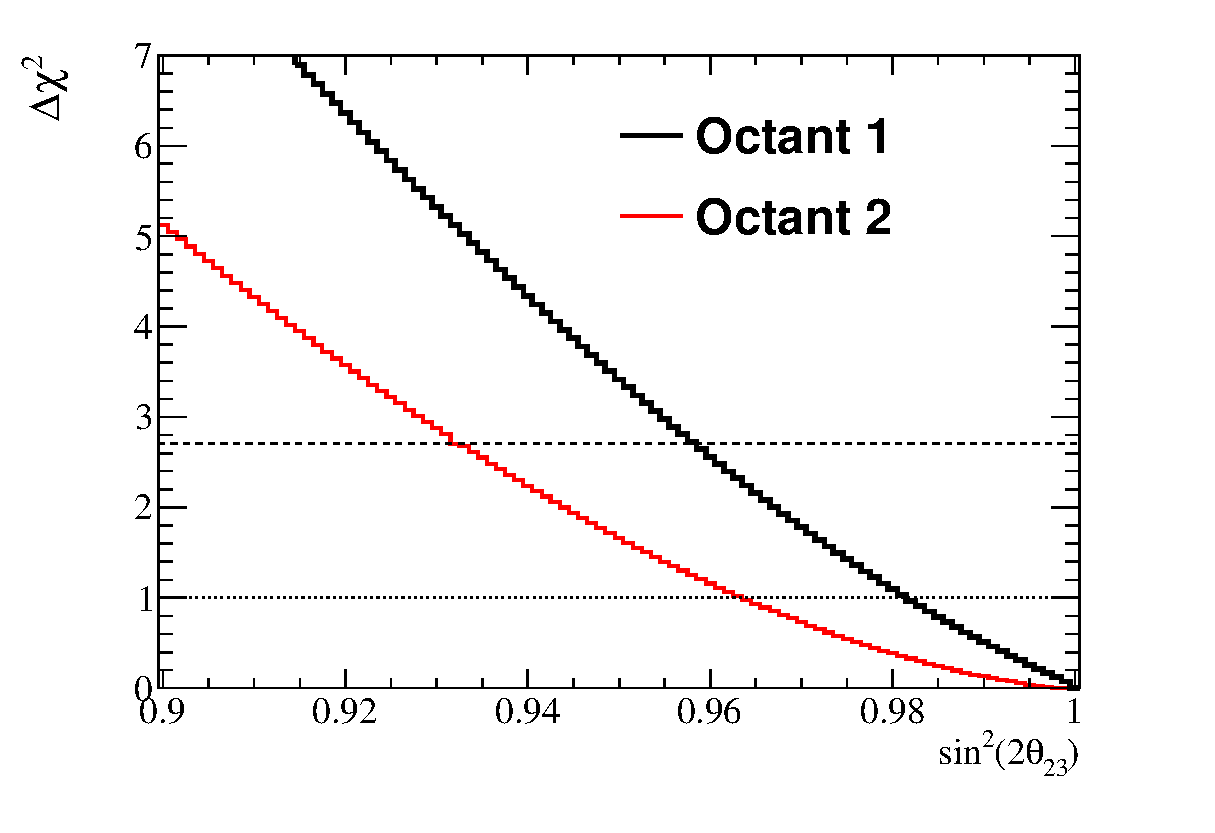
\includegraphics[width=20pc]{./images/fit_data/2N/1D_contour_mixing23_lines}
\caption {$\Delta \chi^2$ as a function of $\sin^22\theta_{23}$
  for the `1+N' fit to the Run 1+2+3 dataset.
  Results are shown for $\theta_{23}$ in for both octants.
  The 68\% and 90\% constant-$\Delta\chi^2$ critical values are shown
  as dotted and dashed lines respectively.
}
\label{fig:results_data123_1dcontour_mixing23}
\end{minipage}
%\vfill
\hspace{0.06\linewidth}
%\begin{minipage}[t]{0.90\linewidth}
\begin{minipage}[t]{0.48\linewidth}
\center
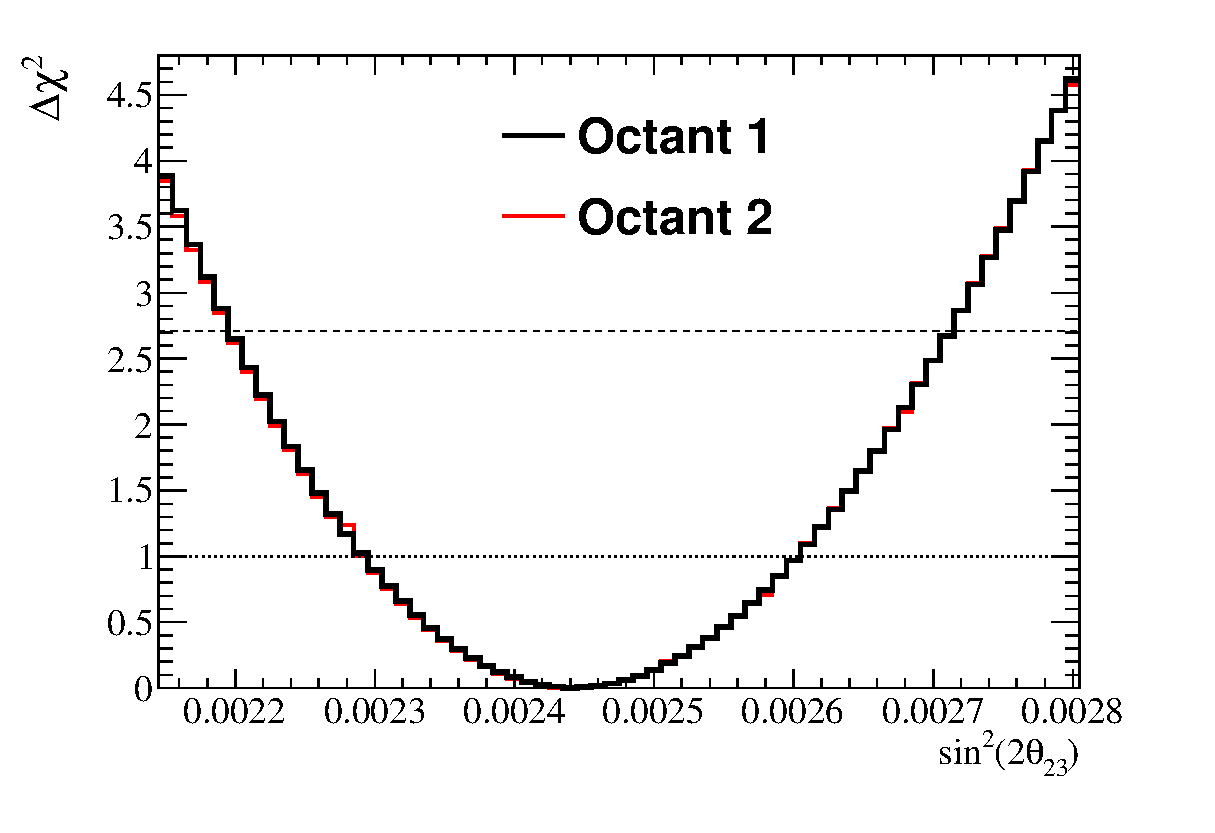
\includegraphics[width=20pc]{./images/fit_data/2N/1D_contour_dm23sq_lines}
\caption { 
  $\Delta \chi^2$ as a function of $|\Delta m^{2}_{32}|$
  for the `1+N' fit to the Run 1+2+3 dataset.
  Results are shown for $\theta_{23}$ in both octants.
  The 68\% and 90\% constant-$\Delta\chi^2$ critical values are shown
  as dotted and dashed lines respectively.
}
\label{fig:results_data123_1dcontour_dm23sq}
\end{minipage}
\end{figure*}


%--------------------------------------------------------------------------------------
% Contours
%--------------------------------------------------------------------------------------

\clearpage

\subsection {Confidence regions}
\label{sec:results_contours}

The first step in constructing confidence contours in the oscillation parameters $\sin^{2}2\theta_{23}$ 
and $|\Delta m^{2}_{32}|$ is to calculate 
the values of $\Delta\chi^2$ for each point in a 2-dimensional grid in the oscillation parameter 
space. This is done as described in Sec.\ \ref{sec:contour_construction_constdchi} for the 
constant-$\Delta\chi^2$ method and in Sec.\ \ref{sec:contour_construction_fc} for the Feldman-Cousins method. 

The $\Delta\chi^2$ surface for the the `2+N' fit for $\sin^2\theta_{23}$ to the Run 1+2+3 dataset is shown in Fig.\
\ref{fig:results_data123_chisq_2Nsintheta}, 
as a function of $\sin^{2}\theta_{23}$ and $|\Delta m^{2}_{32}|$.

The $\Delta\chi^2$ surface for the the `2+N' fit
to the Run 1+2+3 dataset is shown in Figs.\
\ref{fig:results_data123_chisq_2N} and \ref{fig:results_data123_chisq_2NO2}
for $\theta_{23}$ in the first and second octants respectively,
as a function of $\sin^{2}2\theta_{23}$ and $|\Delta m^{2}_{32}|$.
For comparison, the corresponding $\Delta\chi^2$ surfaces for the `2+N' fits to the Run 1+2 and Run 3 
datasets are shown in 
Figs.\ \ref{fig:results_data12_chisq_2N} and \ref{fig:results_data3_chisq_2N} respectively.
The same $\Delta\chi^2$ range is used in all colour plots to allow comparison.
Marginalized $\Delta\chi^2$ distributions are also shown as a function of either $\sin^{2}2\theta_{23}$ 
or $|\Delta m^{2}_{32}|$ for the `2+N' fits to the Run 1+2+3, Run 1+2 and Run 3 datasets in Figs.\ 
\ref{fig:results_marg_dchisq_dmsq_all3_2N} and \ref{fig:results_marg_dchisq_sinsq_all3_2N}
respectively.

The corresponding plots for the `2+8' fits are shown in Fig.\ \ref{fig:results_data123_chisq} for the 
Run 1+2+3 datset, Fig.\ \ref{fig:results_data12_chisq} for the Run 1+2 dataset and Fig.\ 
\ref{fig:results_data3_chisq} for the Run 3 dataset. Meanwhile the marginalized $\Delta\chi^2$ distributions are 
shown for all the datasets as a function of $\sin^{2}2\theta_{23}$ in Fig.\ \ref{fig:results_marg_dchisq_sinsq_all3} 
and as a function of $|\Delta m^{2}_{32}|$ in Fig.\ \ref{fig:results_marg_dchisq_dmsq_all3}.

Comparisons were made between the `2+N' $\Delta\chi^2$ distributions for $\theta_{23}$ in the first and second octants.
The fractional difference between the $\Delta\chi^2$ surfaces
obtained from the `2+N' fits, assuming the first and second octant, to the Run 1+2+3 dataset is shown in 
Fig.\ \ref{fig:results_dchisq_fracdiff_run123_octant}.
% The marginalized $\Delta\chi^2$ distributions 
% for the `2+N' fits, assuming the first and second octant, to the Run 1+2+3 dataset are compared
% as a function of $|\Delta m^{2}_{32}|$ in Fig.\ \ref{fig:results_comp_marg_dchisq_dmsq_run123_octant}
% and as a function of $\sin^{2}2\theta_{23}$ in Fig.\ \ref{fig:results_comp_marg_dchisq_sinsq_run123_octant}. 

Comparisons were made between the `2+N' and `2+8' $\Delta\chi^2$ distributions.
The fractional difference between the $\Delta\chi^2$ surfaces
obtained from the `2+N' and `2+8' fits to the Run 1+2+3 dataset is shown in 
Fig.\ \ref{fig:results_dchisq_fracdiff_run123}. The marginalized $\Delta\chi^2$ distributions 
for the `2+N' and `2+8' fits to the Run 1+2+3 dataset are compared as a function of $|\Delta m^{2}_{32}|$ 
in Fig.\ \ref{fig:results_comp_marg_dchisq_dmsq_run123} and as a function of $\sin^{2}2\theta_{23}$ 
in Fig.\ \ref{fig:results_comp_marg_dchisq_sinsq_run123}. 
As shown in these figures, 
the `2+N' and `2+8' marginalized $\Delta\chi^2$ distributions are almost identical,
even  in areas of the parameter space that exceed the 99\% CL region 
($\Delta\chi^{2} < $ 6.63 for a single parameter).

Confidence regions were constructed using both the constant-$\Delta\chi^2$ method described in 
Sec.\ \ref{sec:contour_construction_constdchi} and the Feldman-Cousins method described in Sec.\ 
\ref{sec:contour_construction_fc} for both the `2+N' and the `2+8' fits. Confidence contours were 
drawn using the constant-$\Delta\chi^2$ method for each of the Run 1+2+3, Run 1+2 and Run 3 datasets. 
Using the Feldman-Cousins method, however, they were drawn only for the Run 1+2+3 dataset 
due to the large amount of CPU time needed.
All confidence regions presented below include the effect of systematic uncertainties.

The 68\% and 90\% CL regions for the `2+N' $\sin^2\theta_{23}$ fit to the Run 1+2+3 dataset are shown using the constant-
$\Delta\chi^2$ method in Fig.\ \ref{fig:results_data123_contour_2Nsintheta}.
The corresponding constant-$\Delta\chi^2$ contours for the
Run 1+2+3 dataset (assuming $\theta_{23}$ is in the first octant),
the Run 1+2+3 dataset (assuming $\theta_{23}$ is in the second octant),
and the Run 1+2 and Run 3 datasets are shown 
in Figs.\ \ref{fig:results_data123_contour_2N}, \ref{fig:results_data123_contour_2NO2},
\ref{fig:results_data12_contour_2N} and \ref{fig:results_data3_contour_2N} respectively. 
The constant-$\Delta\chi^2$ contours for the '2+8' fits 
are shown in Fig.\ \ref{fig:results_data123_contour} for Run 1+2+3, 
in Fig.\ \ref{fig:results_data12_contour} 
for Run 1+2 and in Fig.\ \ref{fig:results_data3_contour} for Run 3.

The Feldman-Cousins 68\% and 90\% CL regions for the fits to the Run 1+2+3 dataset are shown 
in Fig.\ \ref{fig:results_data123_fc_contour_2N} for the `2+N' fit (assuming $\theta_{23}$ is in the first octant),
in Fig.\ \ref{fig:results_data123_fc_contour_2NO2} for the `2+N' fit (assuming $\theta_{23}$ is in the second octant), and
in Fig.\ \ref{fig:results_data123_fc_contour} for the `2+8' fit.
The boundary of the 68\% '2+N' contour assuming $\theta_{23}$ is in the first octant includes the points
($\sin^2(2\theta_{23})$,$|\Delta m^2_{32}|$) =
(1.000,2.64$\times10^{-3}$ eV$^2$/c$^4$), 
(0.964,2.50$\times10^{-3}$ eV$^2$/c$^4$) and
(1.000,2.26$\times10^{-3}$ eV$^2$/c$^4$).
% The boundary of the 90\% '2+N' contour assuming the second octant includes the points
% ($\sin^2(2\theta_{23})$,$|\Delta m^2_{32}|$) =
% (1.000,2.76$\times10^{-3}$ eV$^2$/c$^4$), 
% (0.937,2.50$\times10^{-3}$ eV$^2$/c$^4$) and
% (1.000,2.16$\times10^{-3}$ eV$^2$/c$^4$).

We have accomplished our goal, which was to present the confidence regions
constructed using various methods, and for different fits and datasets.
In the next section, detailed comparisons are presented of the confidence regions obtained 
using different construction methods for the same fit, and 
using different fitting methods for the same construction method.
The contours from different running periods are compared, and we also compare our contours
from the fits to the combined Run 1+2+3 dataset with recent measurements from MINOS and SuperK
and T2K 3.010$\times$10$^{20}$-POT sensitivity contours. 
Finally, a more critical view of the 5 different results obtained by
this analysis is presented in Sec.\ \ref{sec:primary_result_selection}.

%...........................................................
%
% \Delta\chisquare surfaces for `2+N' fits
%
\begin{figure*}[htb]
\center
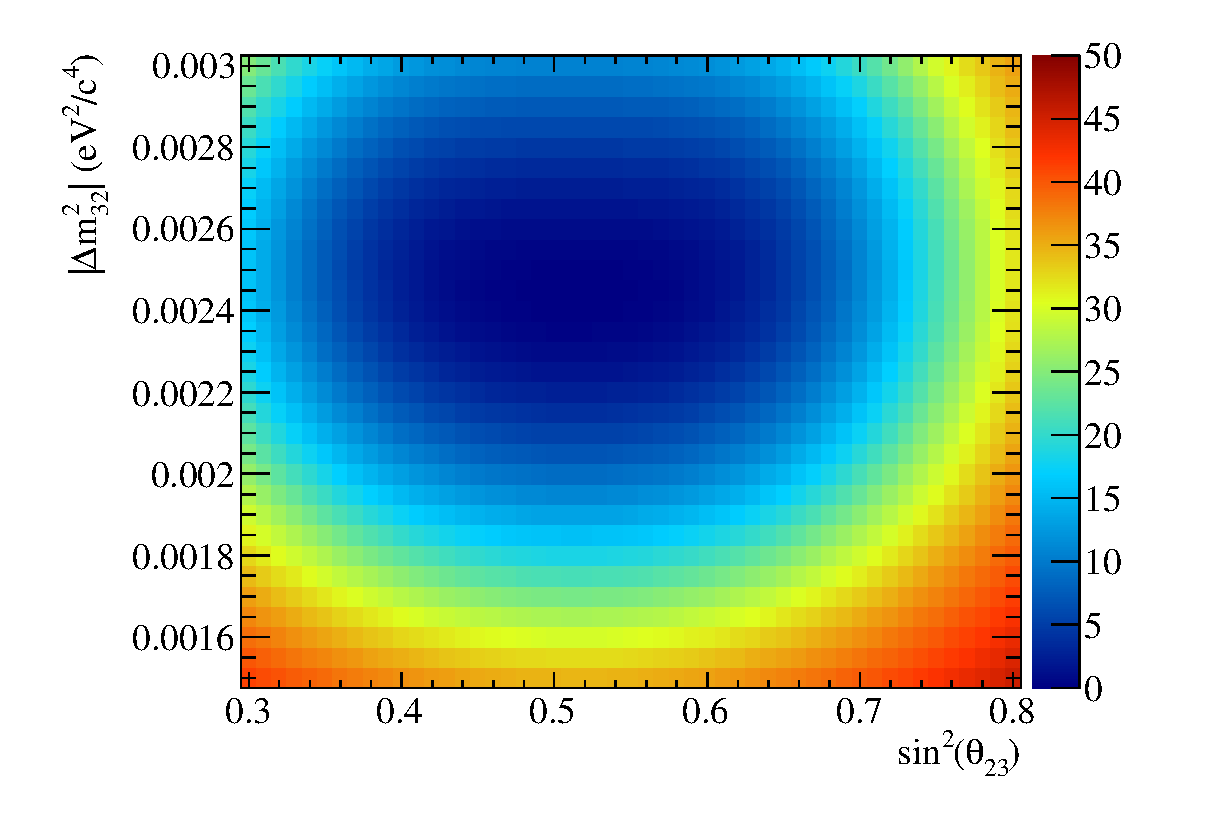
\includegraphics[width=21pc]{./images/fit_data/2Nsintheta/dchisq_3}
\caption {
  $\Delta\chi^2$ surface for the `2+N' $\sin^2\theta_{23}$ fit to the Run 1+2+3 dataset.
}
\label{fig:results_data123_chisq_2Nsintheta}
\end{figure*}

\begin{figure*}[htb]
\begin{minipage}[t]{0.48\linewidth}
\center
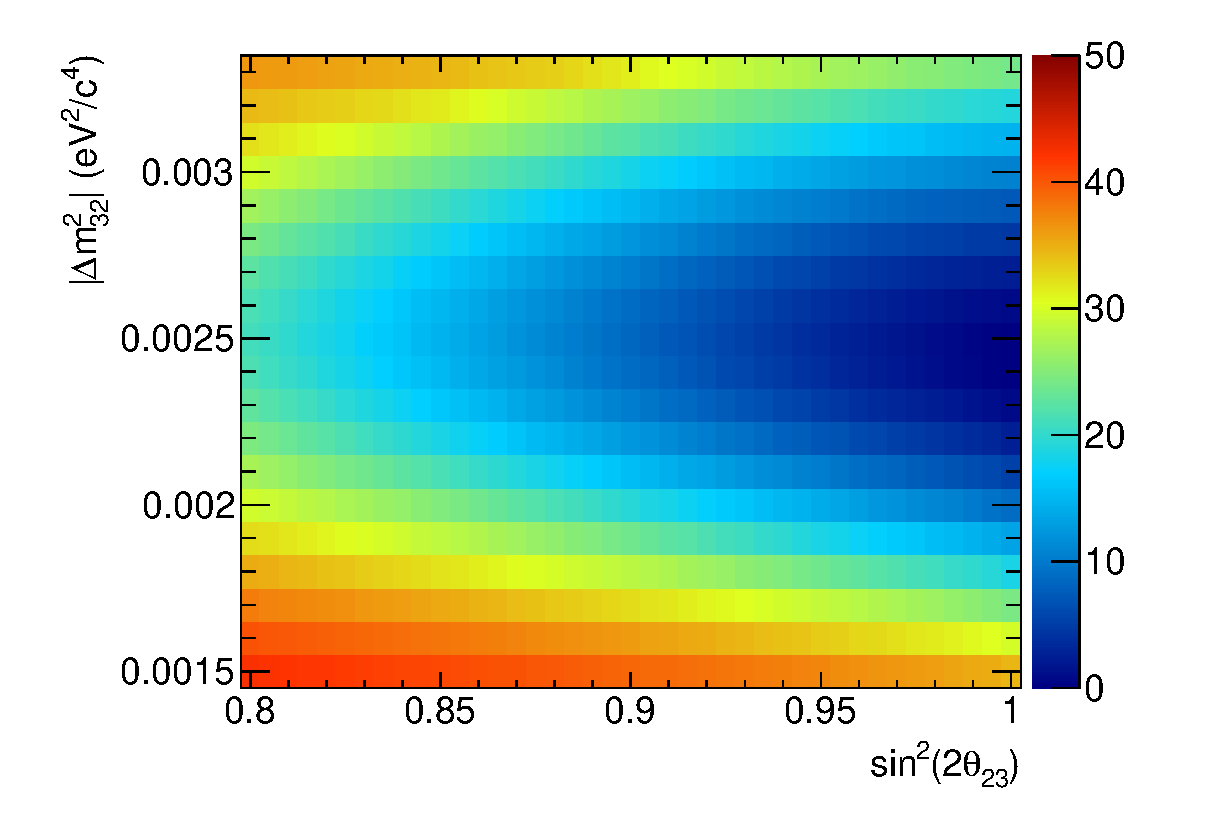
\includegraphics[width=21pc]{./images/fit_data/2N/dchisq_3}
\caption {
  $\Delta\chi^2$ surface for the `2+N' fit to the Run 1+2+3 dataset, assuming $\theta_{23}$ is in the first octant.
}
\label{fig:results_data123_chisq_2N}
\end{minipage}
\hspace{0.06\linewidth}
\begin{minipage}[t]{0.48\linewidth}
\center
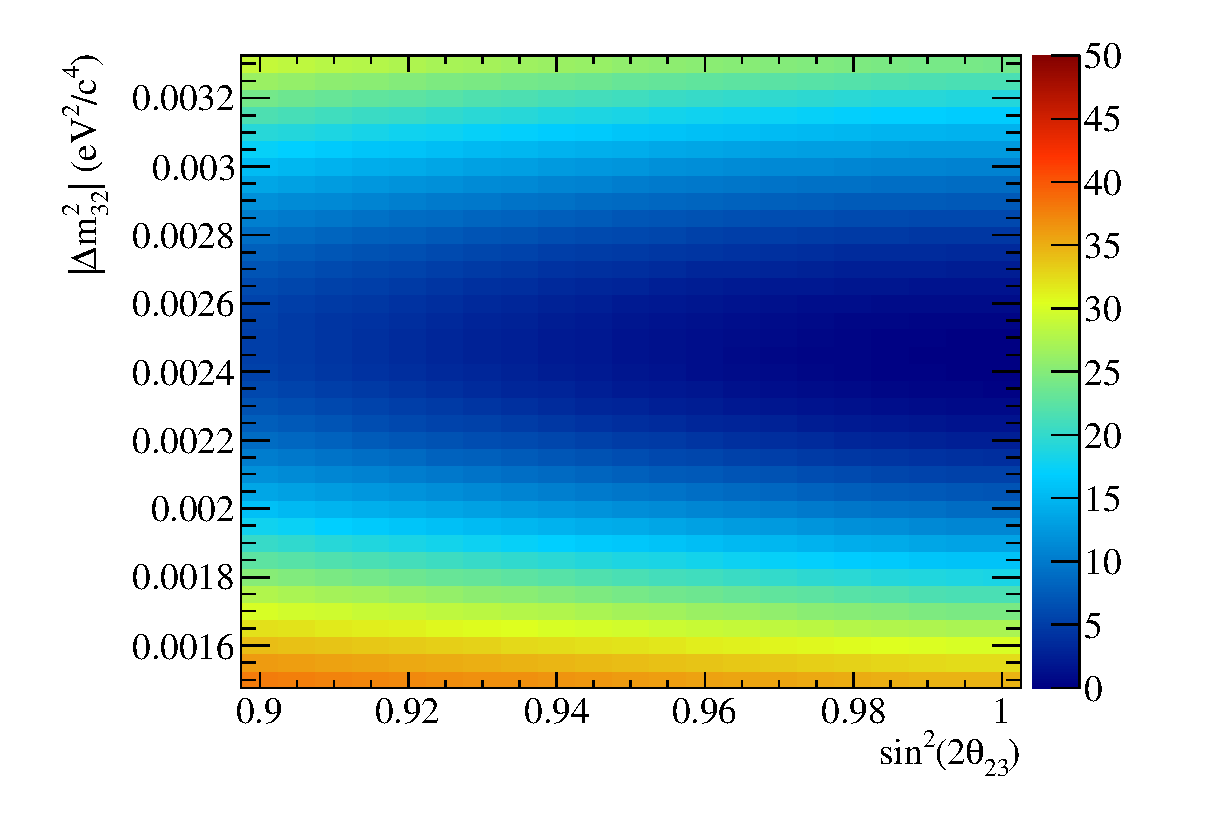
\includegraphics[width=21pc]{./images/fit_data/2Noctant2/dchisq_3}
\caption {
  $\Delta\chi^2$ surface for the `2+N' fit to the Run 1+2+3 dataset, assuming $\theta_{23}$ is in the second octant.
}
\label{fig:results_data123_chisq_2NO2}
\end{minipage}
\end{figure*}

\begin{figure*}[htb]
\begin{minipage}[t]{0.48\linewidth}
\center
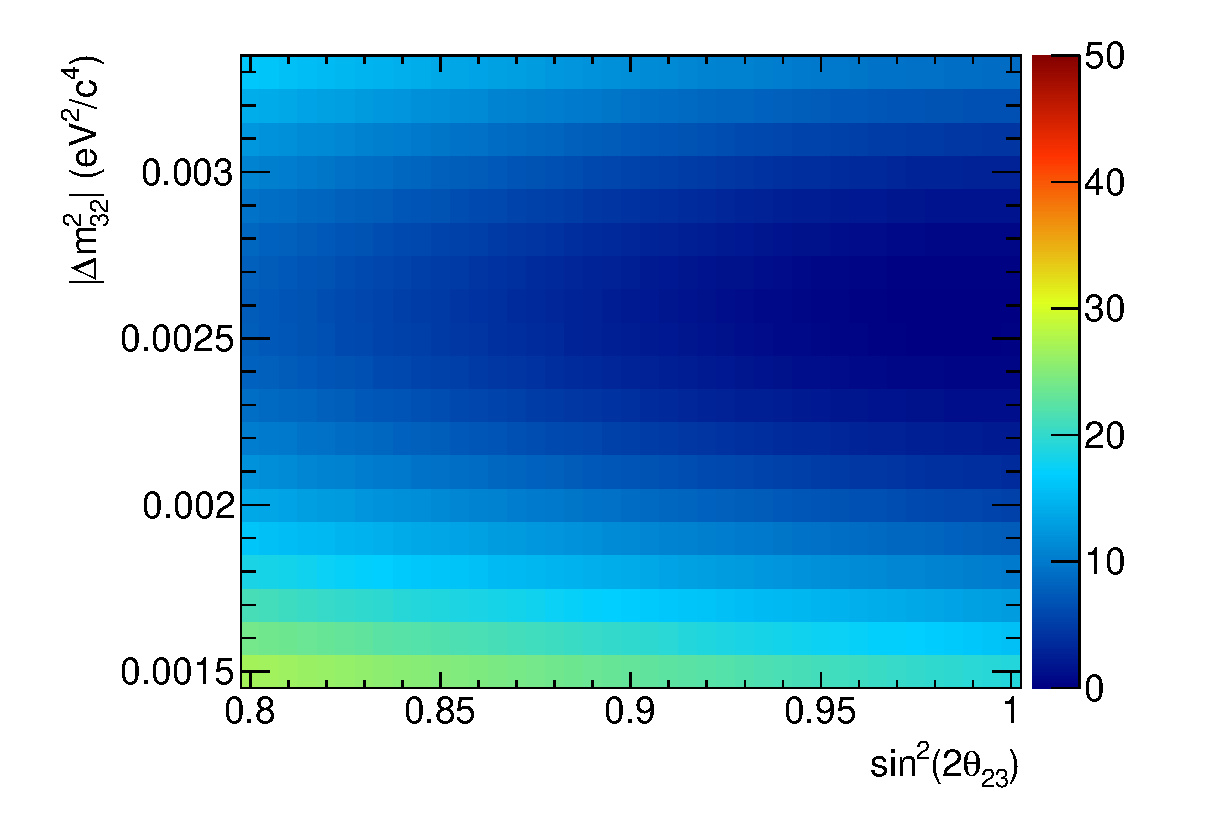
\includegraphics[width=21pc]{./images/fit_data/2N/dchisq_4}
\caption {
  $\Delta\chi^2$ surface for the `2+N' fit to the Run 1+2 dataset.
}
\label{fig:results_data12_chisq_2N}
\end{minipage}
\hspace{0.06\linewidth}
\begin{minipage}[t]{0.48\linewidth}
\center
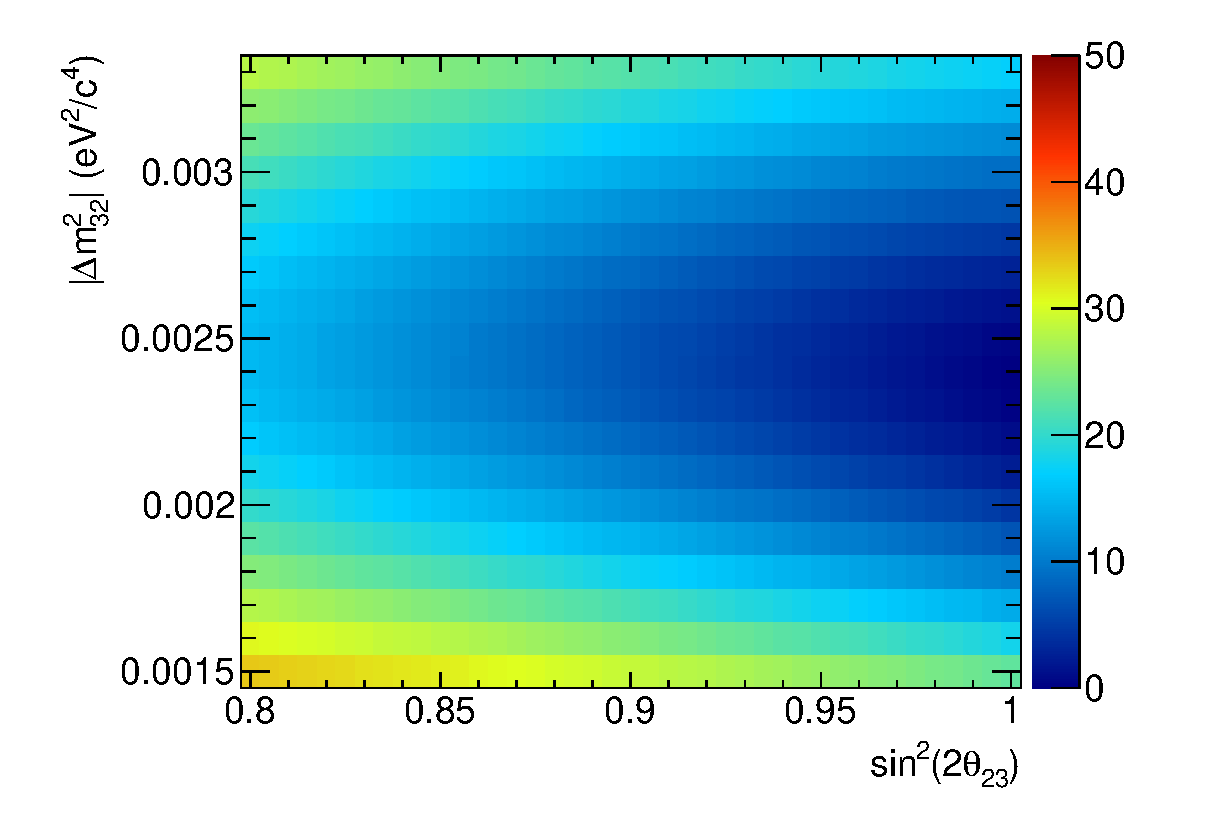
\includegraphics[width=21pc]{./images/fit_data/2N/dchisq_5}
\caption {
  $\Delta\chi^2$ surface for the `2+N' fit to the Run 3 dataset.
}
\label{fig:results_data3_chisq_2N}
\end{minipage}
\end{figure*}

%...........................................................
%
% Marginalised \Delta\chisquare plots for `2+N' fits
%
\begin{figure*}[htb]
\center
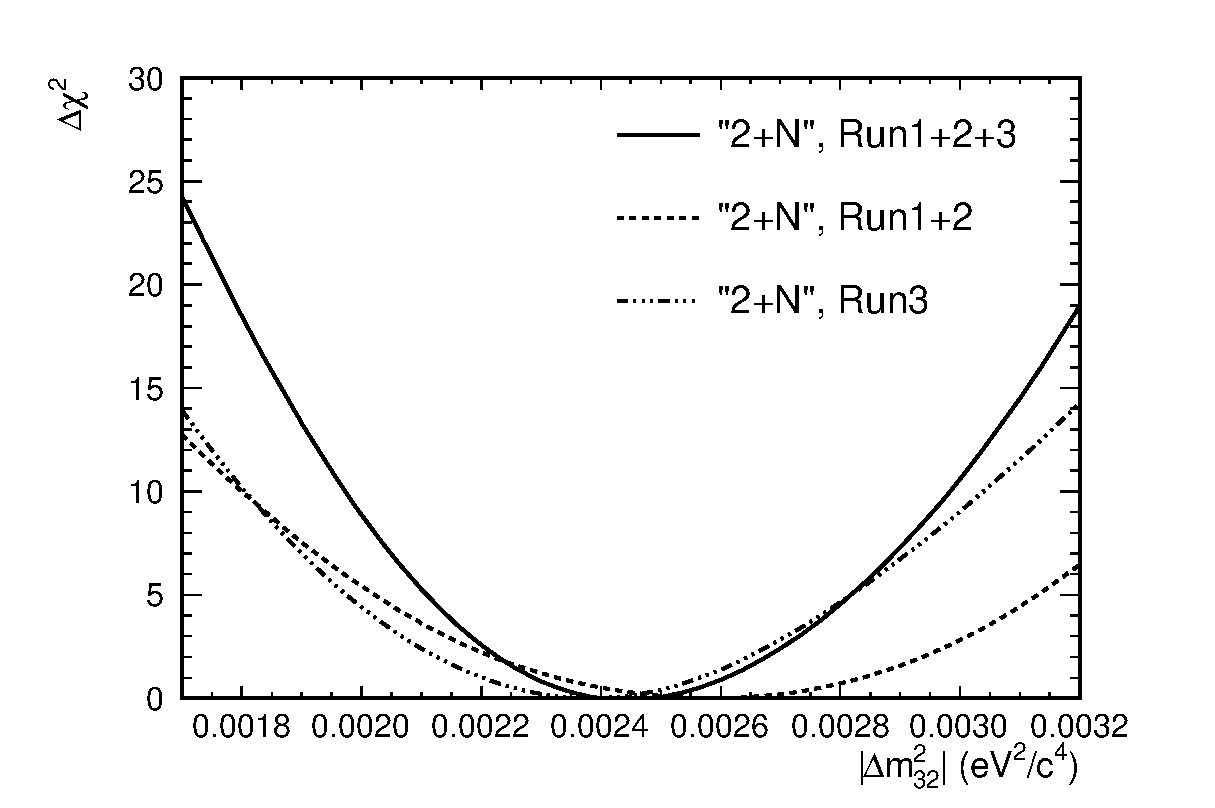
\includegraphics[width=35pc]{./images/fit_data/2N/marg_dchisq_withsyst_dm32sq_2N.eps}
\caption {
  Marginalized $\Delta\chi^2$, as a function of $|\Delta m^{2}_{32}|$, 
  for the four `2+N' fits to the Run 1+2+3, Run 1+2 and Run 3 datasets.
}
\label{fig:results_marg_dchisq_dmsq_all3_2N}
\end{figure*}

\begin{figure*}[htb]
\center
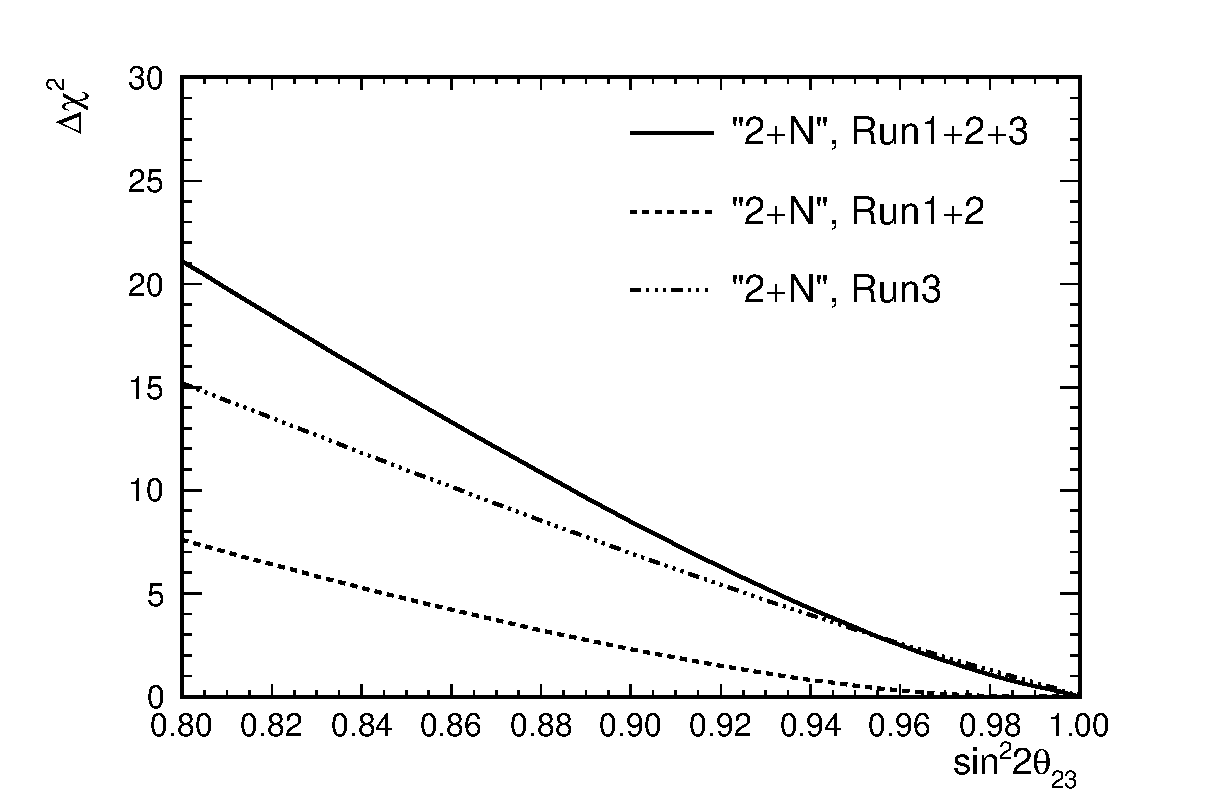
\includegraphics[width=35pc]{./images/fit_data/2N/marg_dchisq_withsyst_sinsq23_2N.eps}
\caption {
  Marginalized $\Delta\chi^2$, as a function of $\sin^{2}2\theta_{23}$, 
  for the three `2+N' fits to the Run 1+2+3, Run 1+2 and Run 3 datasets.
}
\label{fig:results_marg_dchisq_sinsq_all3_2N}
\end{figure*}


%...........................................................
%
% \Delta\chisquare surfaces for `2+8' fits
%
\begin{figure*}[htb]
\center
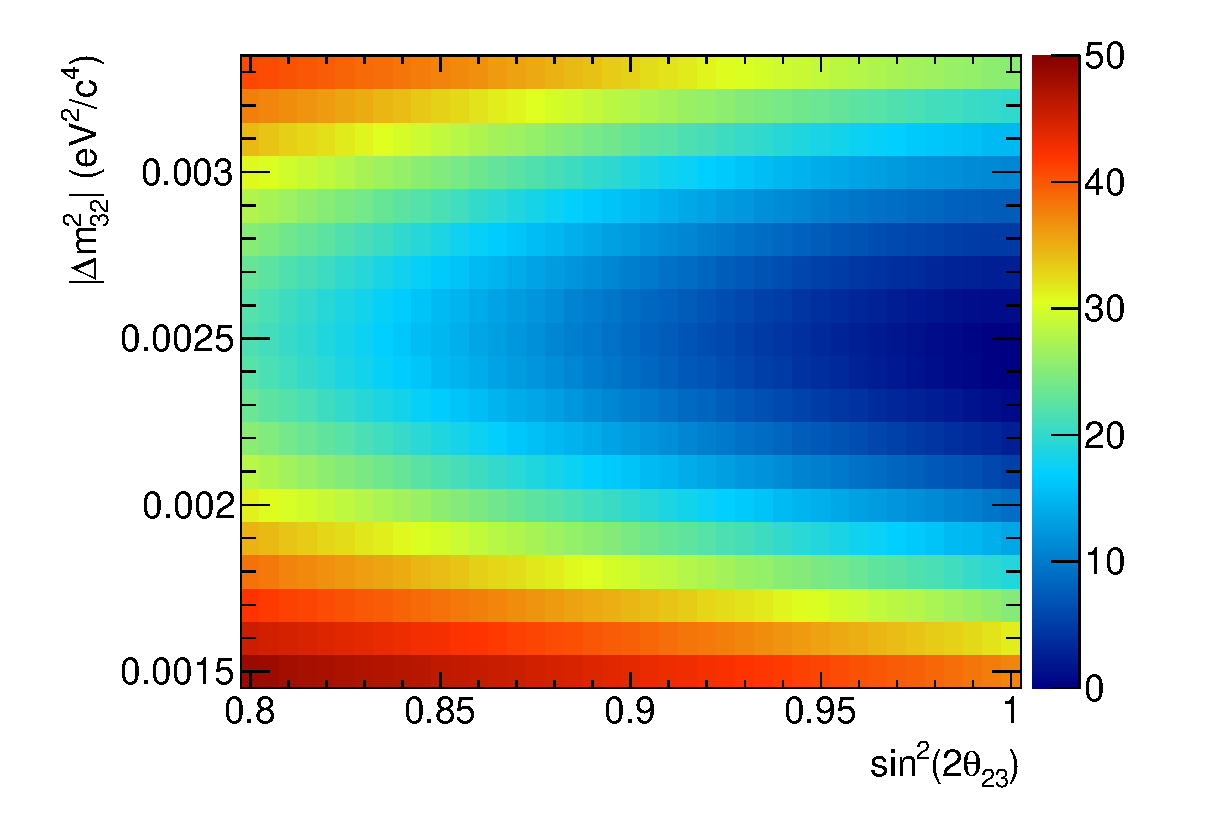
\includegraphics[width=36pc]{./images/fit_data/28/dchisq_3}
\caption {
  $\Delta\chi^2$ surface for the `2+8' fit to the Run 1+2+3 dataset.
}
\label{fig:results_data123_chisq}
\end{figure*}

\begin{figure*}[htb]
\begin{minipage}[t]{0.48\linewidth}
\center
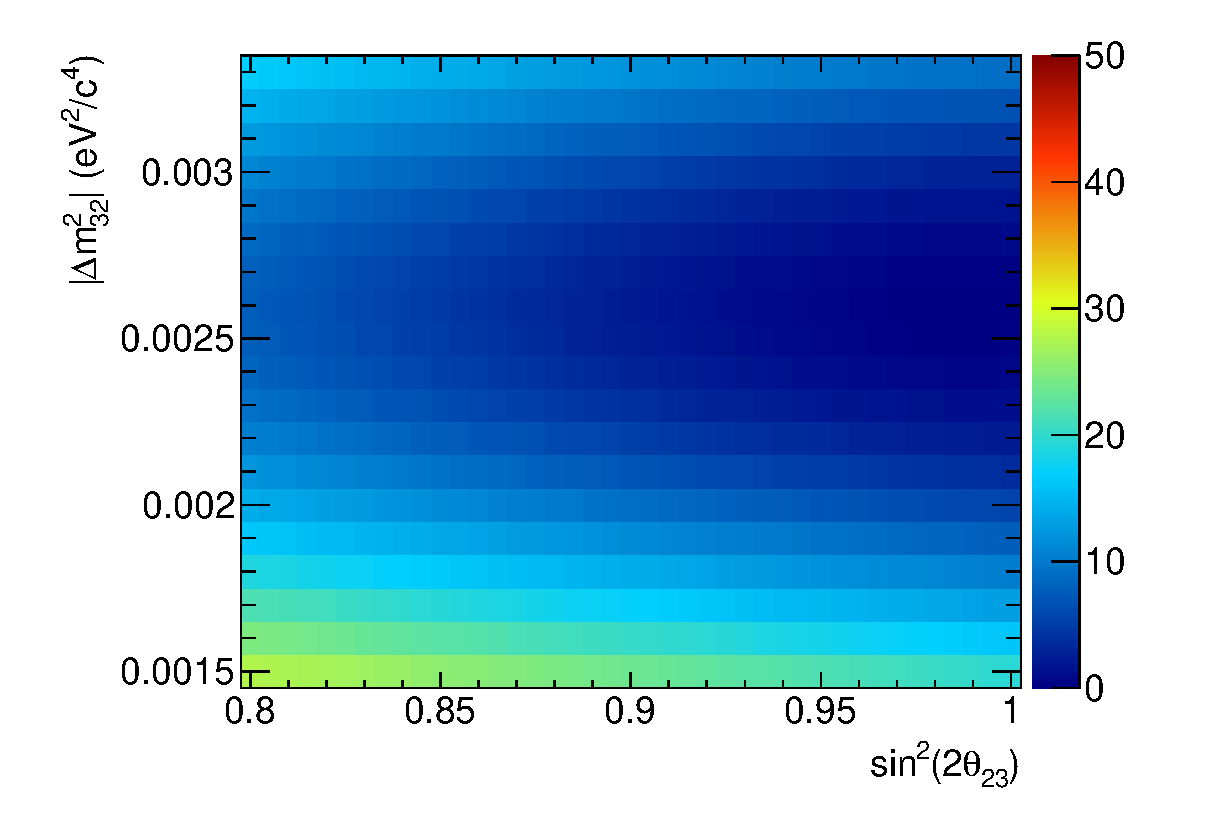
\includegraphics[width=21pc]{./images/fit_data/28/dchisq_4}
\caption {
  $\Delta\chi^2$ surface for the `2+8' fit to the Run 1+2 dataset.
}
\label{fig:results_data12_chisq}
\end{minipage}
\hspace{0.06\linewidth}
\begin{minipage}[t]{0.48\linewidth}
\center
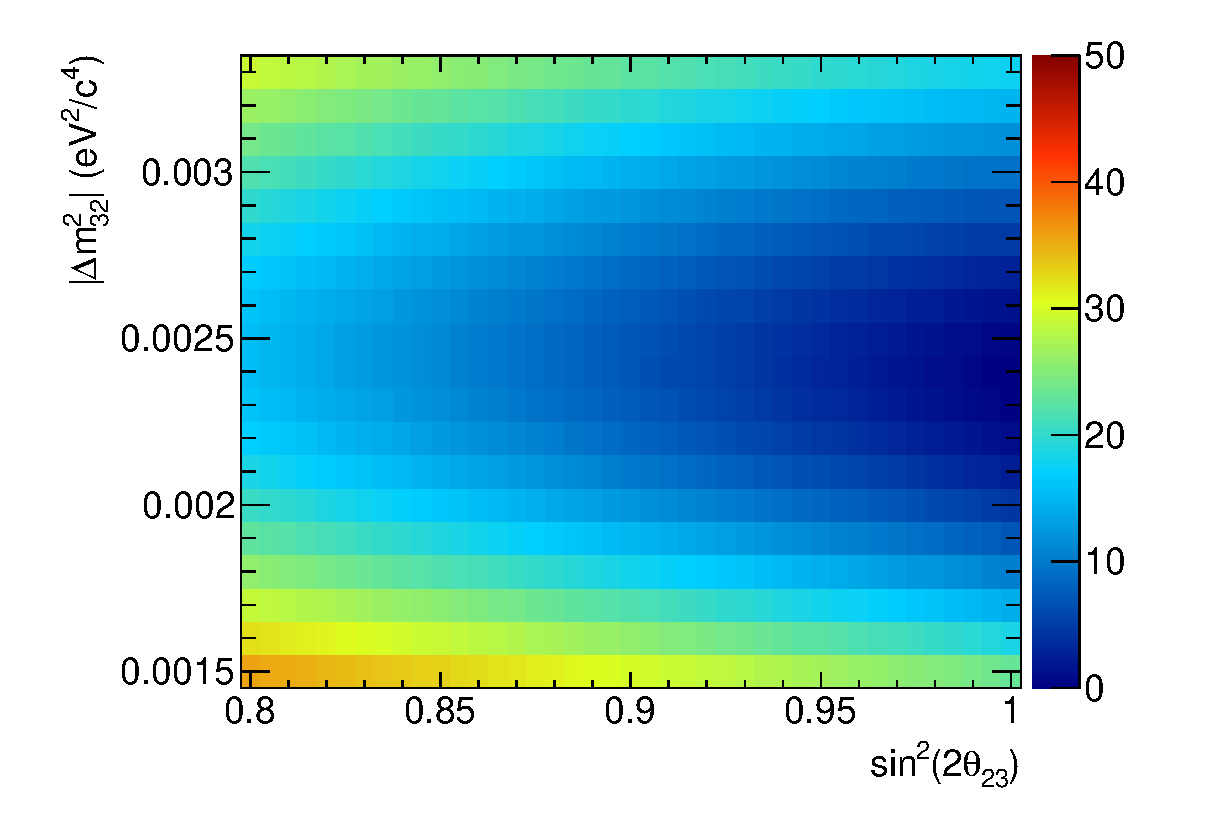
\includegraphics[width=21pc]{./images/fit_data/28/dchisq_5}
\caption {
  $\Delta\chi^2$ surface for the `2+8' fit to the Run 3 dataset.
}
\label{fig:results_data3_chisq}
\end{minipage}
\end{figure*}

%...........................................................
%
% Marginalised \Delta\chisquare plots for `2+8' fits
%
\begin{figure*}[htb]
\center
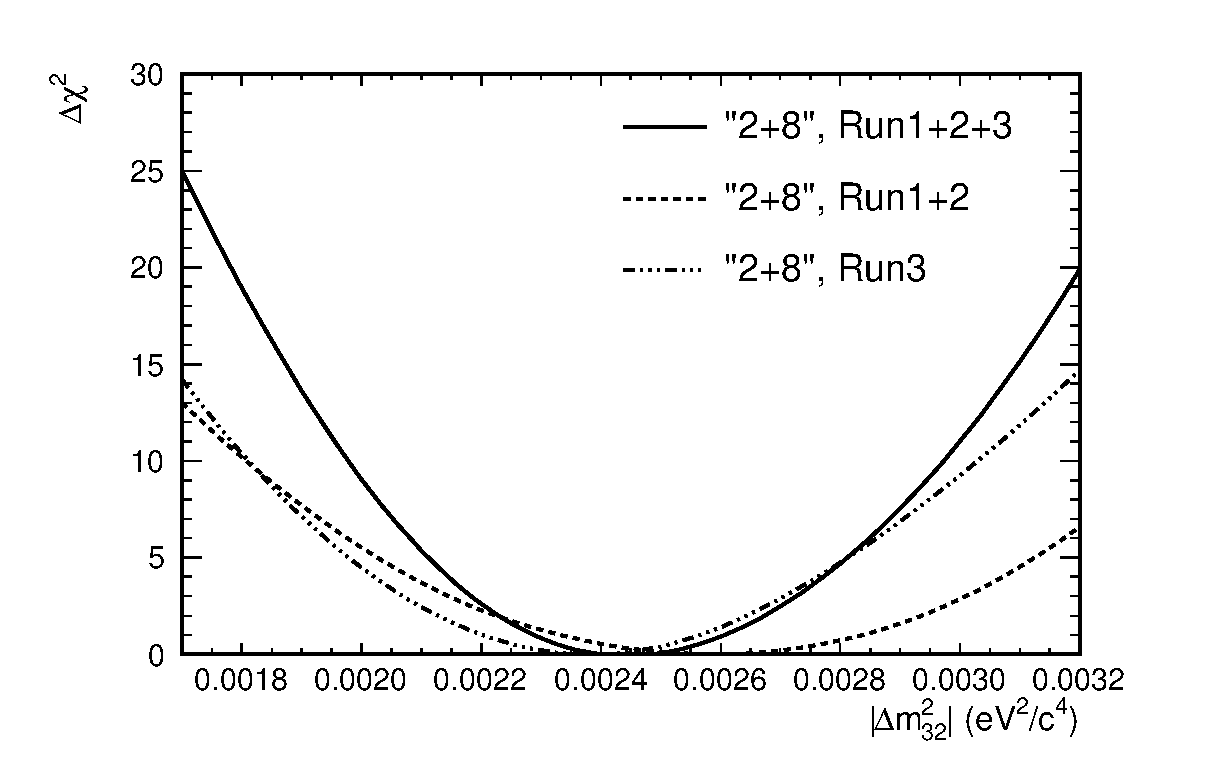
\includegraphics[width=35pc]{./images/fit_data/28/marg_dchisq_withsyst_dm32sq_28.eps}
\caption {
  Marginalized $\Delta\chi^2$, as a function of $|\Delta m^{2}_{32}|$, 
  for the three `2+8' fits to the Run 1+2+3, Run 1+2 and Run 3 datasets.
}
\label{fig:results_marg_dchisq_dmsq_all3}
\end{figure*}

\begin{figure*}[htb]
\center
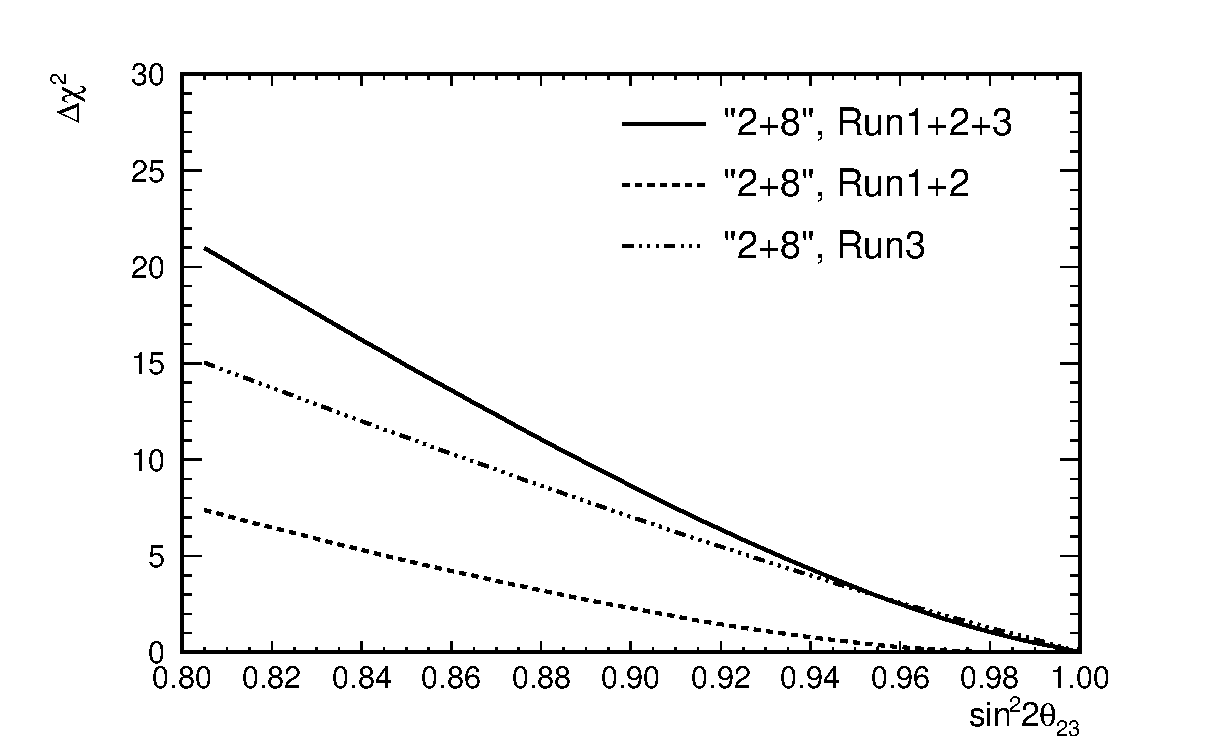
\includegraphics[width=35pc]{./images/fit_data/28/marg_dchisq_withsyst_sinsq23_28.eps}
\caption {
  Marginalized $\Delta\chi^2$, as a function of $\sin^{2}2\theta_{23}$, 
  for the three `2+8' fits to the Run 1+2+3, Run 1+2 and Run 3 datasets.
}
\label{fig:results_marg_dchisq_sinsq_all3}
\end{figure*}

%...........................................................
%
% Comparison of `2+N' first and second octant
% \Delta\chisquare surfaces and
% marginalised \Delta\chisquare distributions
%

\begin{figure*}[htb]
%\begin{minipage}[t]{0.48\linewidth}
\center
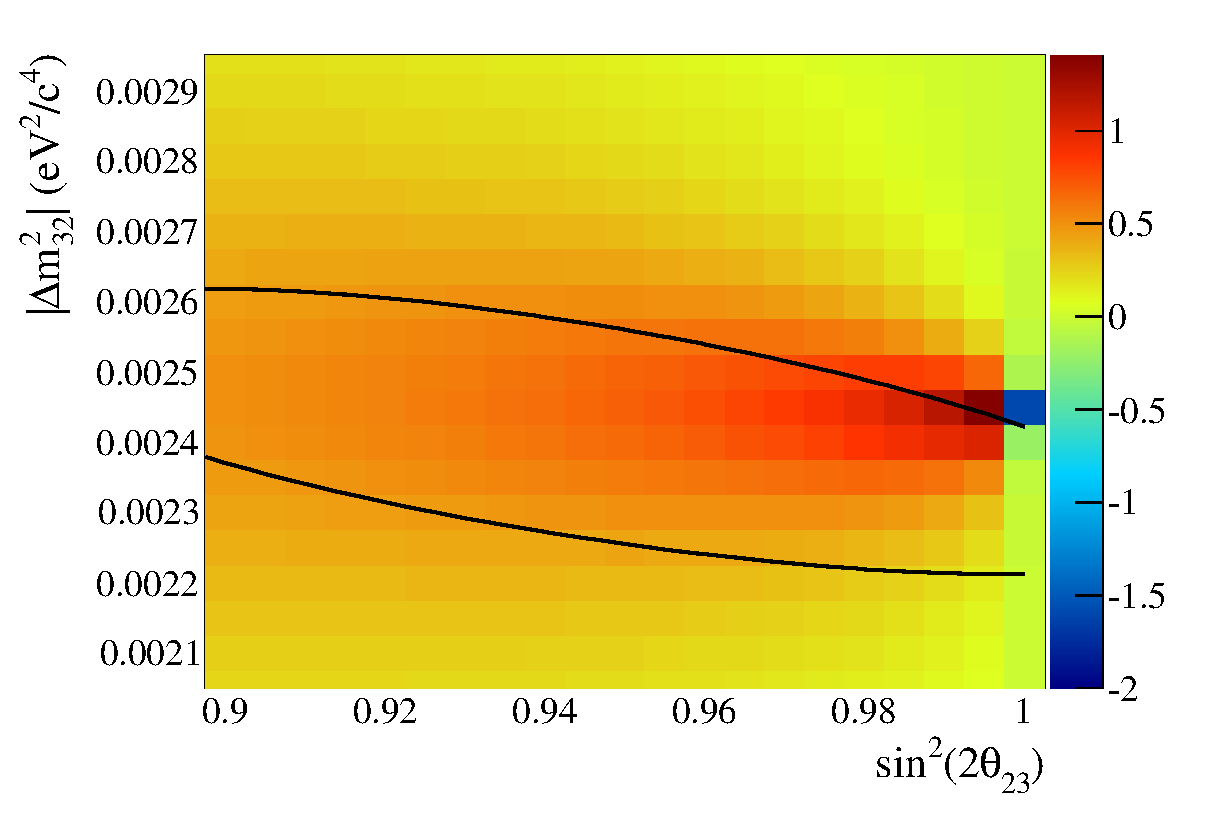
\includegraphics[width=20pc]{./images/fit_data/compare/compare_octants_dchisqdiff_nM8OnP8O2}
\caption {
  Fractional difference between the $\Delta\chi^2$ surfaces
  obtained from the `2+N' fits to the Run 1+2+3 dataset assuming $\theta_{23}$ is in the first and second octants
  and shown in Figs.\ \ref{fig:results_data123_chisq_2N} and \ref{fig:results_data123_chisq_2NO2}.
  The fractional difference is calculated as 
  2 $\times$ ($\Delta\chi^2$(octant 1)-$\Delta\chi^2$(octant 2)) / $\Delta\chi^2$(octant 1)+$\Delta\chi^2$(octant 2)).
  The 2012 MINOS 90\% CL region is shown for reference.
  The large difference at the minimum of the $\Delta \chi^2$ maps is due to the best fit point in the
  second octant case being further away from a bin center.
}
\label{fig:results_dchisq_fracdiff_run123_octant}
%\end{minipage}
% \hspace{0.06\linewidth}
% \begin{minipage}[t]{0.48\linewidth}
% \center
% % \includegraphics[width=20pc]{./images/fit_data/compare/compare_octants_dchisqdiff_nM8OnP8O2_zoom}
% 
\includegraphics[width=20pc]{./images/placeholder}
% \caption {
%   As on the left but zoomed into the area of the 2012 MINOS 90\% CL region.
% }
% \label{fig:results_dchisq_fracdiff_run123_octant_zoom}
% \end{minipage}
\end{figure*}

%---

% \begin{figure*}[htb]
% \begin{minipage}[t]{0.48\linewidth}
% \center
% 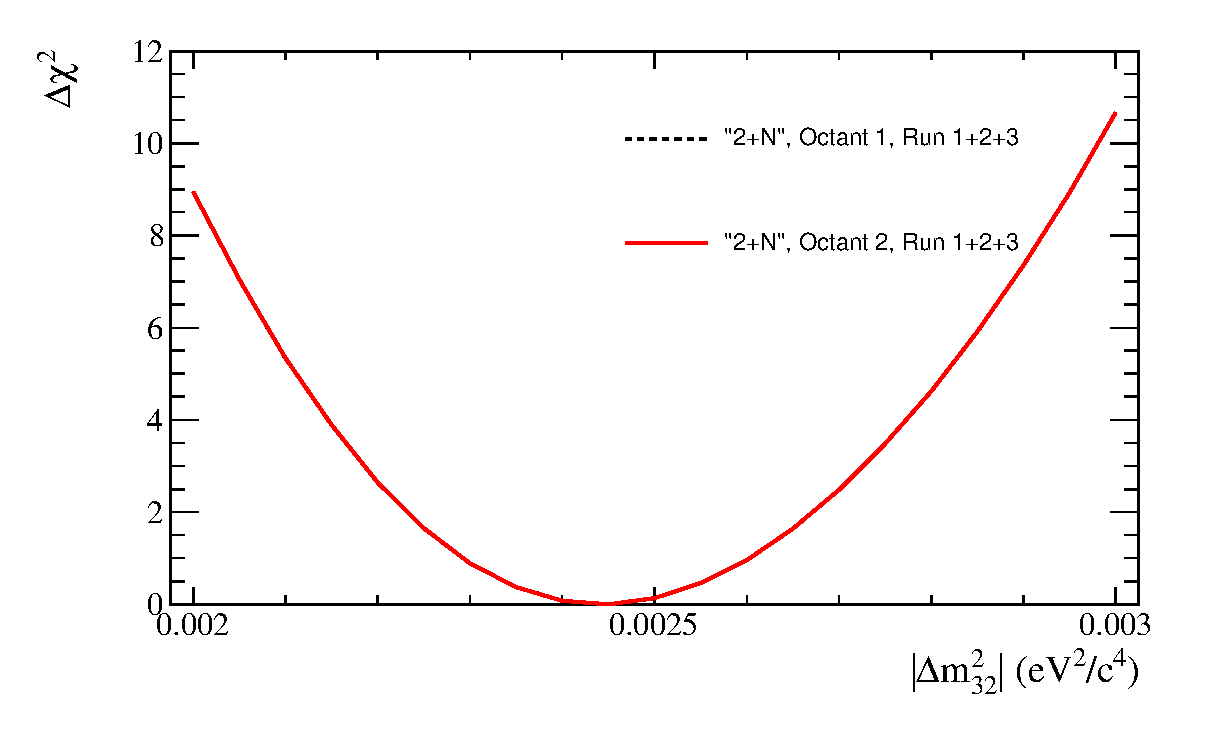
\includegraphics[width=20pc]{./images/fit_data/compare/marg_dchisq_withsyst_dm23sq_2N_2NO2_comp.eps}
% \caption {
%   Comparison of marginalized $\Delta\chi^2$ as a function of $|\Delta m^{2}_{32}|$, 
%   for the `2+N' fits to the Run 1+2+3 dataset, for both octant assumptions.
% }
% \label{fig:results_comp_marg_dchisq_dmsq_run123_octant}
% \end{minipage}
% \hspace{0.06\linewidth}
% \begin{minipage}[t]{0.48\linewidth}
% \center
% 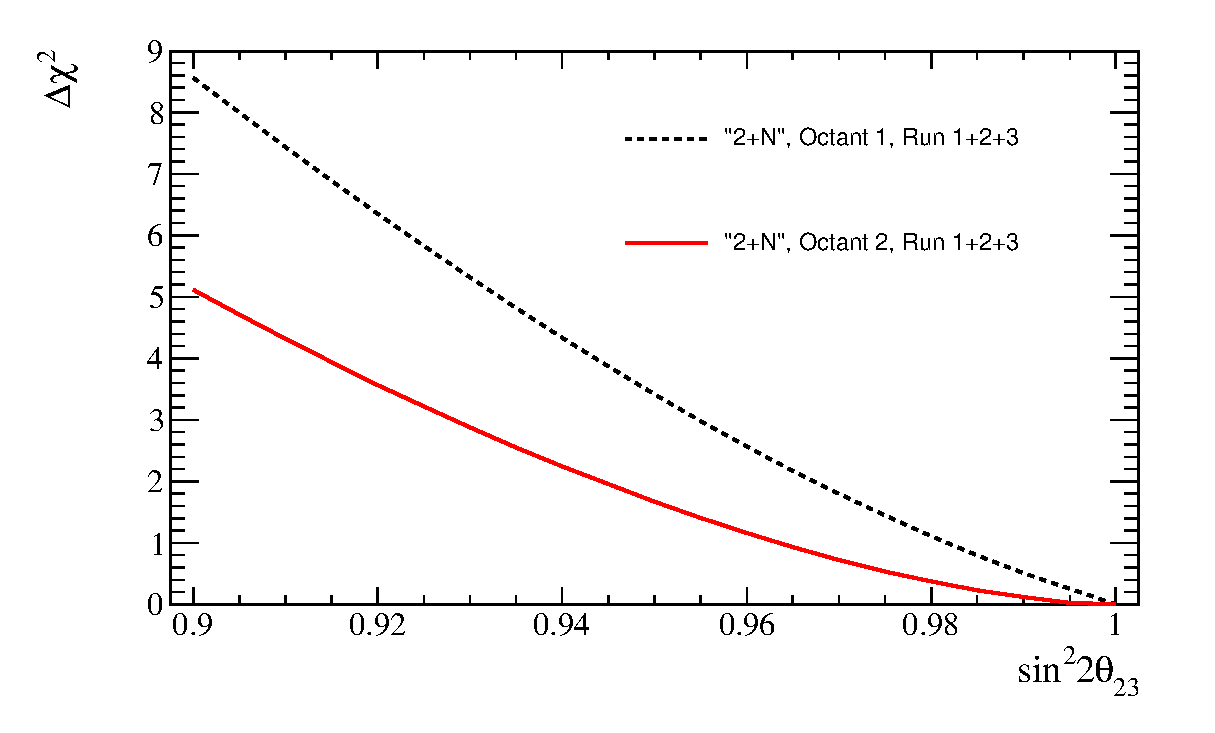
\includegraphics[width=20pc]{./images/fit_data/compare/marg_dchisq_withsyst_sinsq23_2N_2NO2_comp.eps}
% \caption {
%   Comparison of marginalized $\Delta\chi^2$ as a function of $\sin^{2}2\theta_{23}$, 
%   for the `2+N' fits to the Run 1+2+3 dataset, for both octant assumptions.
% }
% \label{fig:results_comp_marg_dchisq_sinsq_run123_octant}
% \end{minipage}
% \end{figure*}


%...........................................................
%
% Comparison of `2+N' and `2+8' 
% \Delta\chisquare surfaces and
% marginalised \Delta\chisquare distributions
%

\begin{figure*}[htb]
\begin{minipage}[t]{0.48\linewidth}
\center
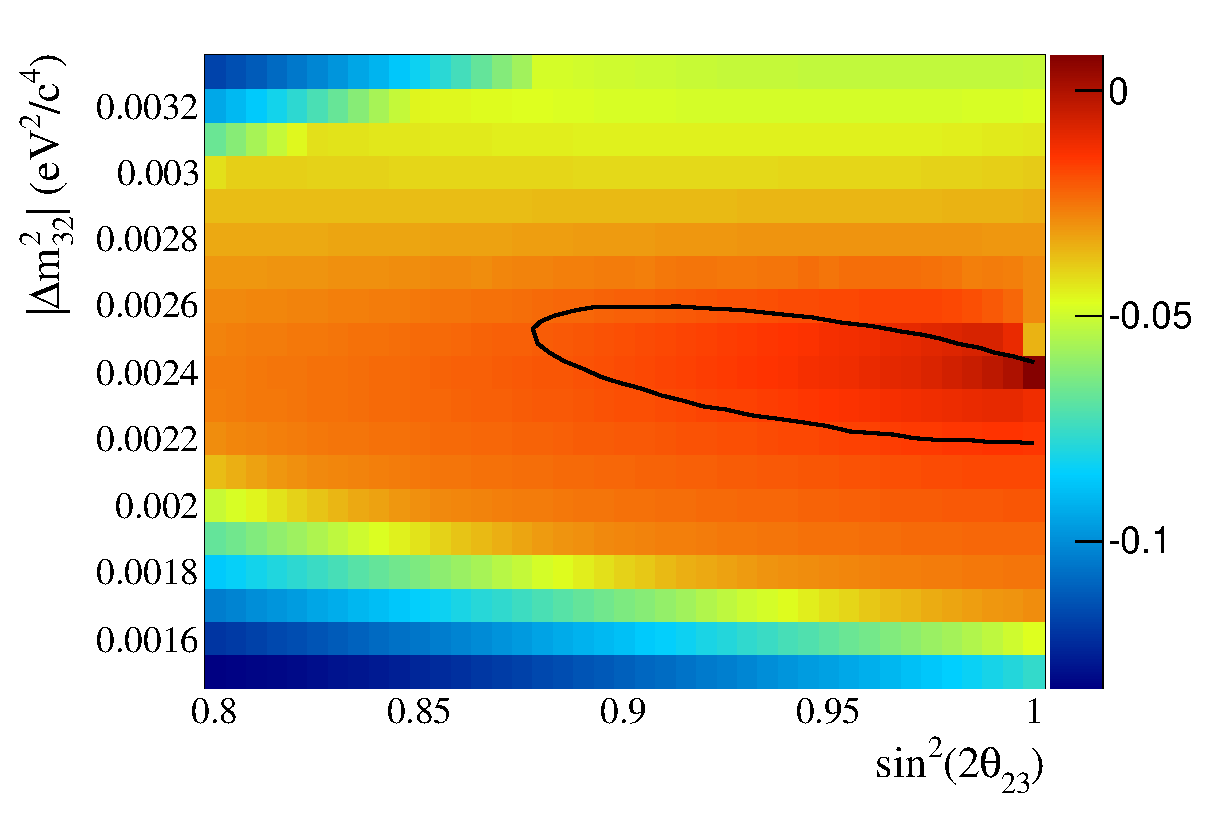
\includegraphics[width=20pc]{./images/fit_data/compare/compare_2all_28_dchisqdiff_nM8OnP8O2}
\caption {
  Fractional difference between the $\Delta\chi^2$ surfaces
  obtained from the `2+N' and `2+8' fits to the Run 1+2+3 dataset 
  and shown in Figs.\ \ref{fig:results_data123_chisq_2N} and \ref{fig:results_data123_chisq}.
  The fractional difference is calculated as 
  2 $\times$ ($\Delta\chi^2$(`2+N')-$\Delta\chi^2$(`2+8')) / $\Delta\chi^2$(`2+N')+$\Delta\chi^2$(`2+8')).
  The 2012 MINOS 90\% CL region is shown for reference.
}
\label{fig:results_dchisq_fracdiff_run123}
\end{minipage}
\hspace{0.06\linewidth}
\begin{minipage}[t]{0.48\linewidth}
\center
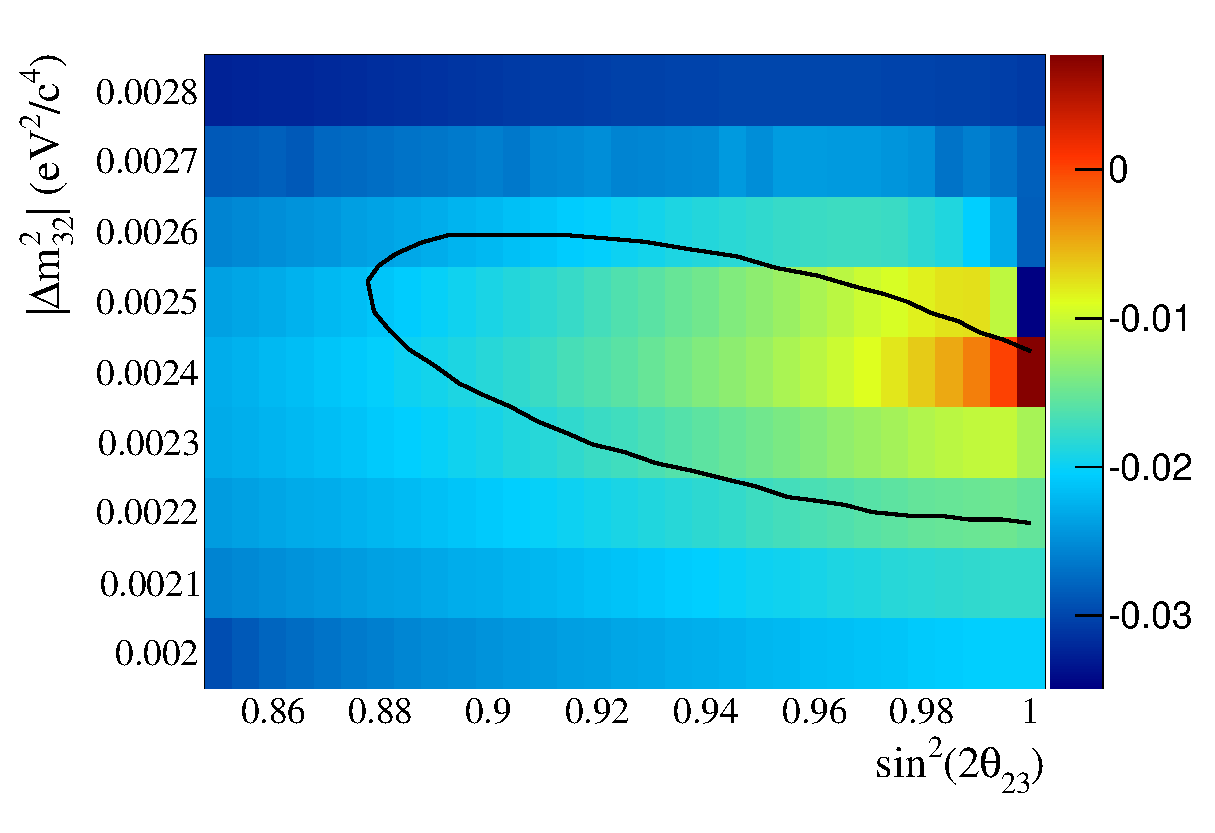
\includegraphics[width=20pc]{./images/fit_data/compare/compare_2all_28_dchisqdiff_nM8OnP8O2_zoom} 
\caption {
  As on the left but zoomed into the area of the 2012 MINOS 90\% CL region.
}
\label{fig:results_dchisq_fracdiff_run123_zoom}
\end{minipage}
\end{figure*}

%---

\begin{figure*}[htb]
\begin{minipage}[t]{0.48\linewidth}
\center
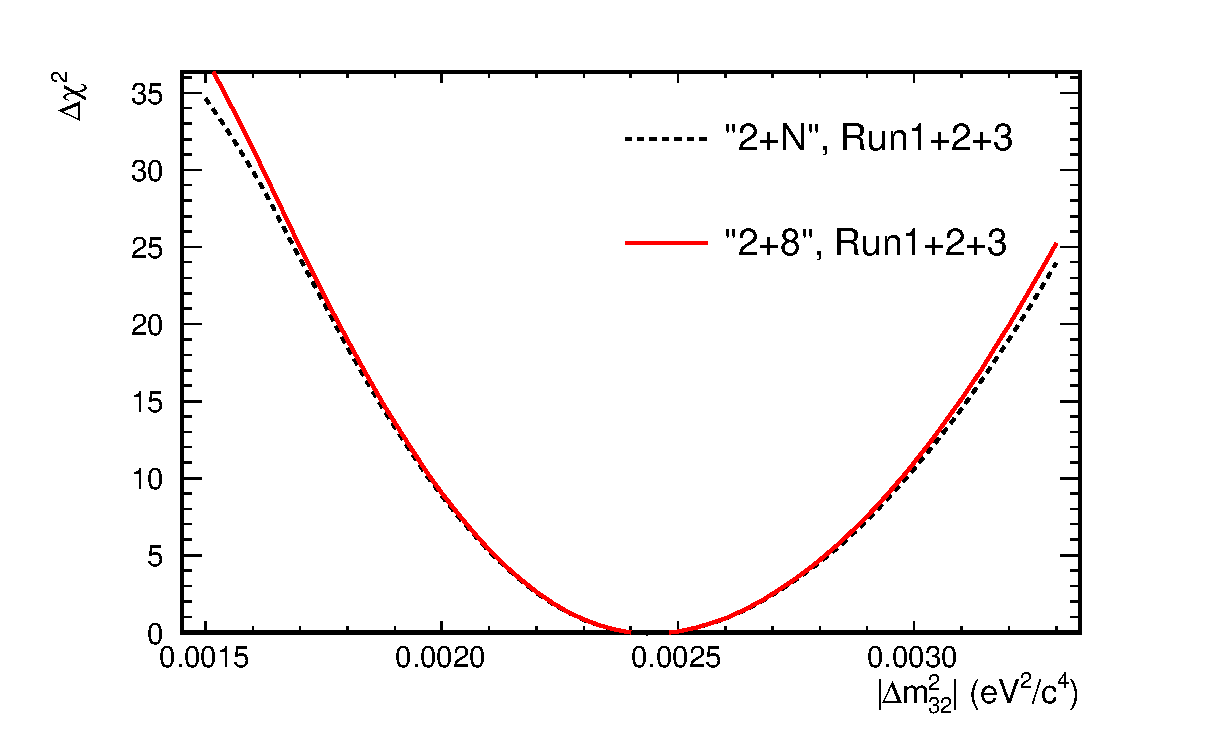
\includegraphics[width=20pc]{./images/fit_data/compare/marg_dchisq_withsyst_dm23sq_2N_28_comp.eps}
\caption {
  Comparison of marginalized $\Delta\chi^2$ as s function of $|\Delta m^{2}_{32}|$, 
  for the `2+N' and `2+8' fits to the Run 1+2+3 dataset.
}
\label{fig:results_comp_marg_dchisq_dmsq_run123}
\end{minipage}
\hspace{0.06\linewidth}
\begin{minipage}[t]{0.48\linewidth}
\center
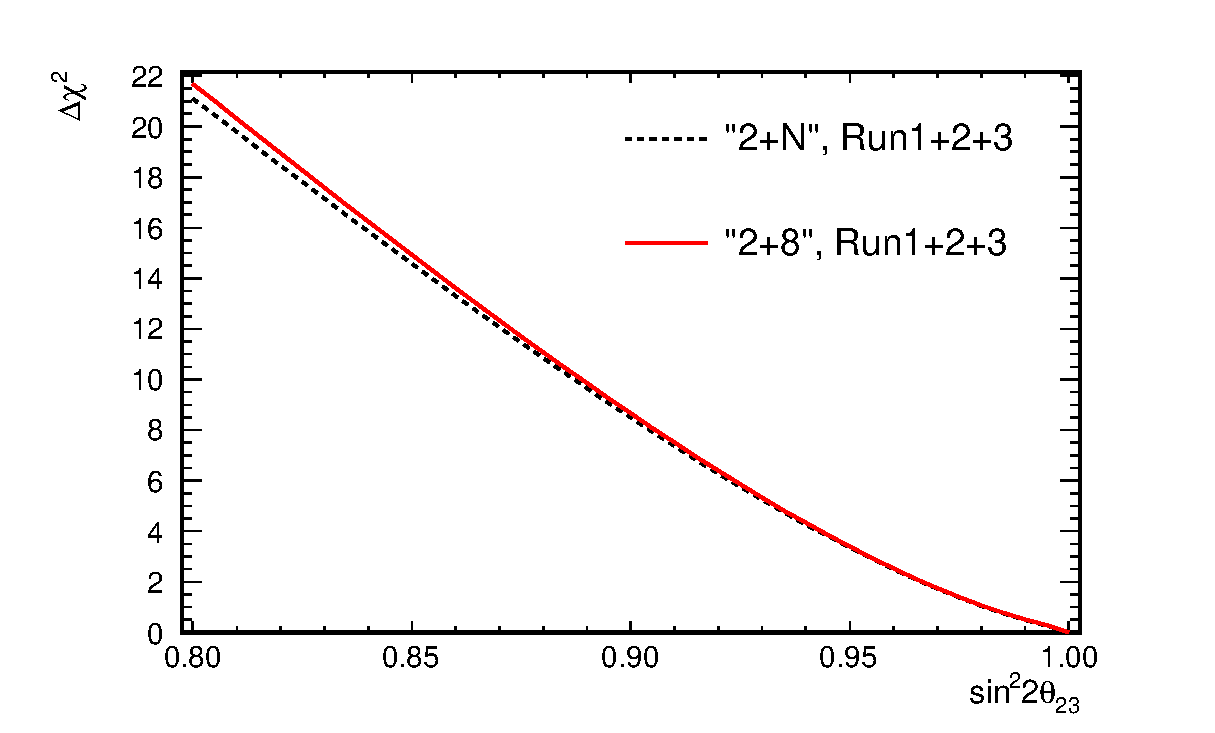
\includegraphics[width=20pc]{./images/fit_data/compare/marg_dchisq_withsyst_sinsq23_2N_28_comp.eps}
\caption {
  Comparison of marginalized $\Delta\chi^2$ as a function of $\sin^{2}2\theta_{23}$, 
  for the `2+N' and `2+8' fits to the Run 1+2+3 dataset.
}
\label{fig:results_comp_marg_dchisq_sinsq_run123}
\end{minipage}
\end{figure*}

%...........................................................
%
% Const-dchi^2  contours for `2+N' fits
%

\clearpage

\begin{figure*}[htb]
\center
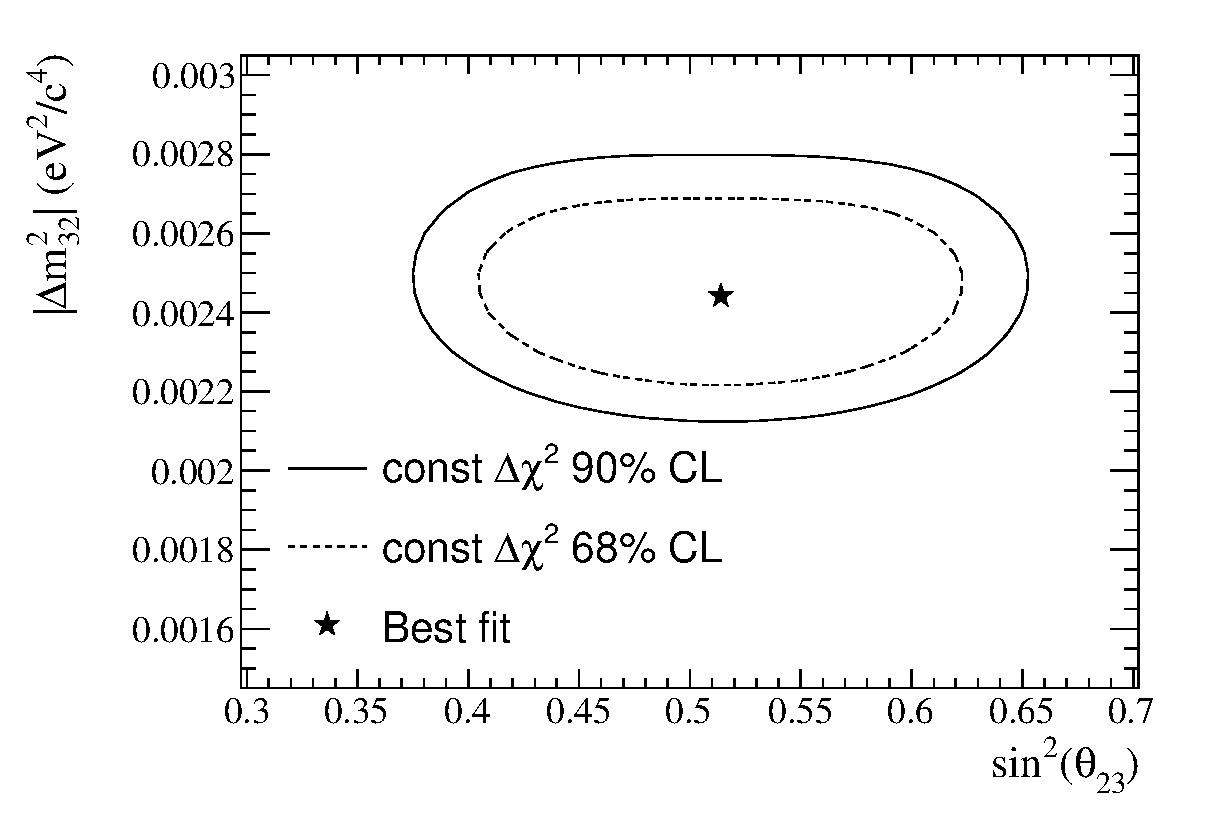
\includegraphics[width=30pc]{./images/fit_data/2Nsintheta/contours_3}
\caption {
  68\% CL and 90\% CL allowed region (including systematics), 
  constructed with the constant-$\Delta\chi^{2}$ method,
  for the `2+N' $\sin^2\theta_{23}$ fit to the Run 1+2+3 dataset.
  The `2+N' best-fit point is also shown.
}
\label{fig:results_data123_contour_2Nsintheta}
\end{figure*}


\begin{figure*}[htb]
\center
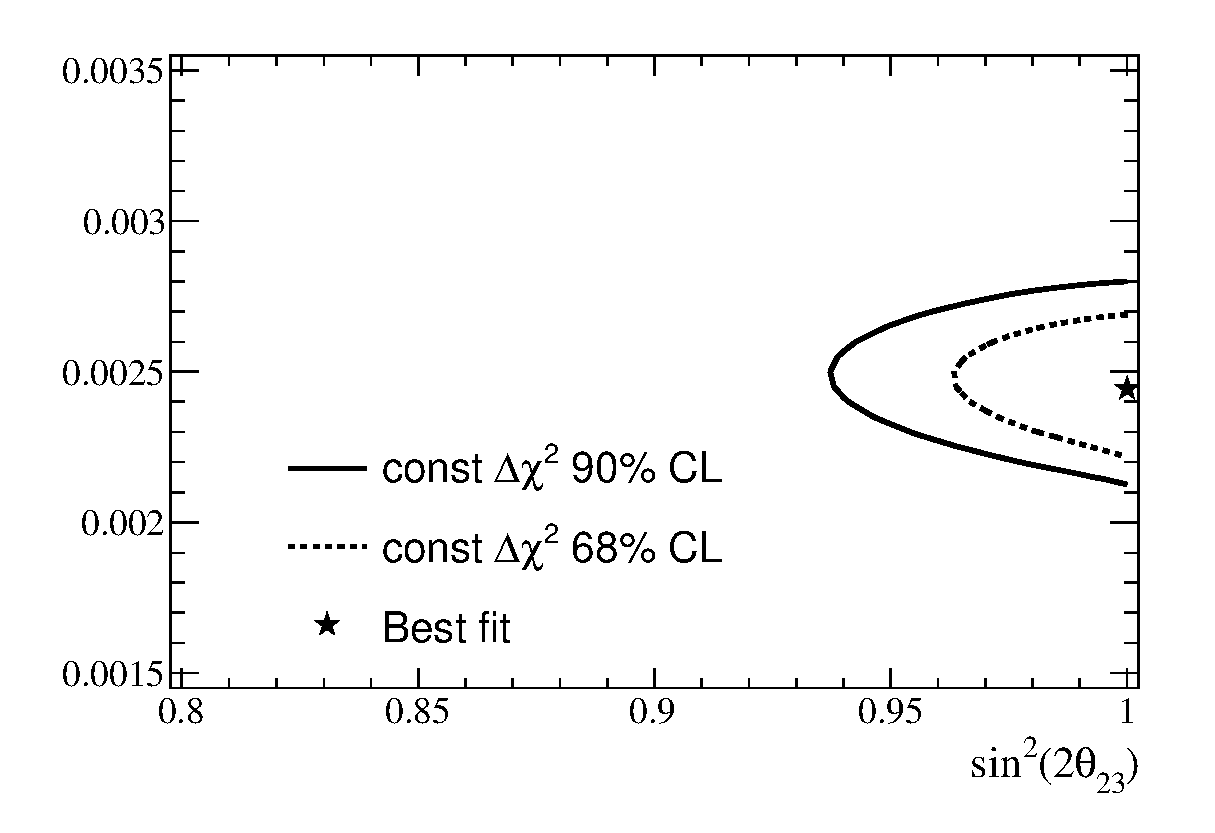
\includegraphics[width=30pc]{./images/fit_data/2N/contours_3}
\caption {
  68\% CL and 90\% CL allowed region (including systematics), 
  constructed with the constant-$\Delta\chi^{2}$ method,
  for the `2+N' fit to the Run 1+2+3 dataset assuming $\theta_{23}$ is in the first octant.
  The `2+N' best-fit point is also shown.
}
\label{fig:results_data123_contour_2N}
\end{figure*}

\begin{figure*}[htb]
\center
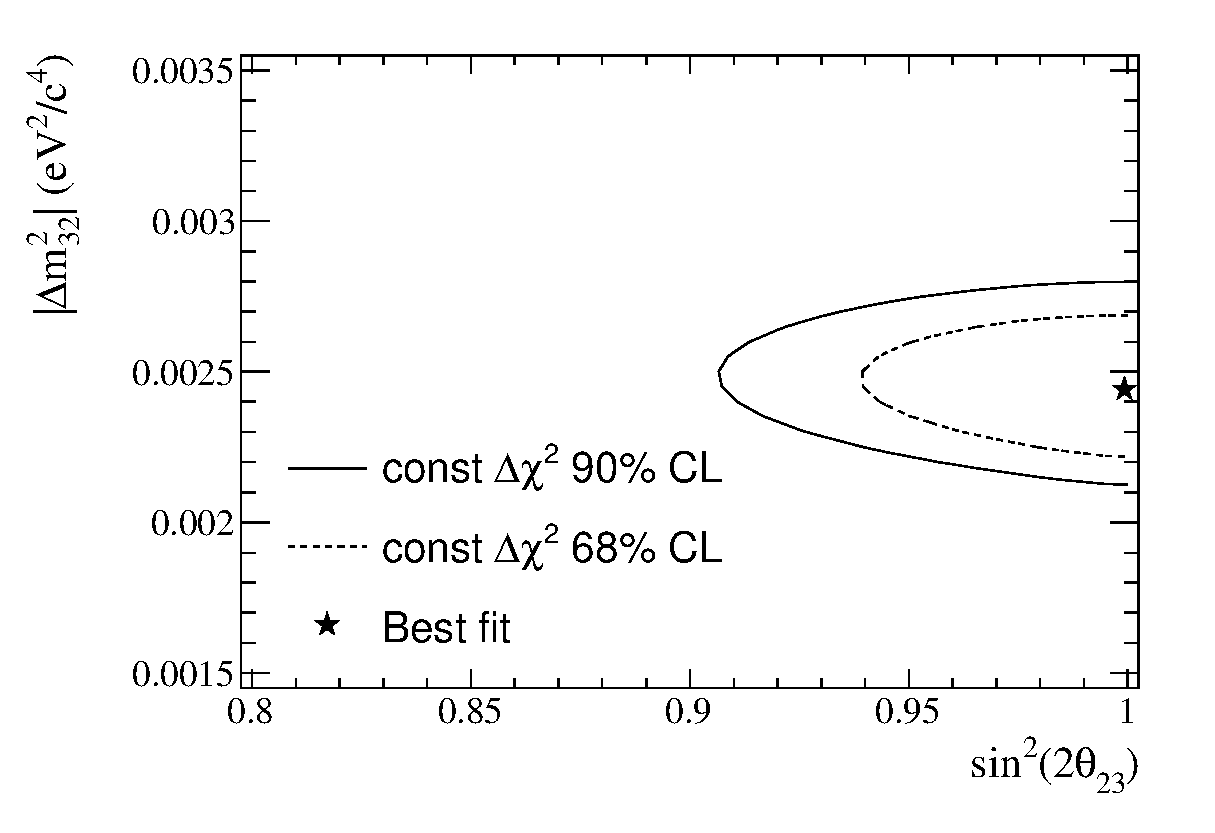
\includegraphics[width=30pc]{./images/fit_data/2Noctant2/contours_3}
\caption {
  68\% CL and 90\% CL allowed region (including systematics), 
  constructed with the constant-$\Delta\chi^{2}$ method,
  for the `2+N' fit to the Run 1+2+3 dataset assuming $\theta_{23}$ is in the second octant.
  The `2+N' best-fit point is also shown.
}
\label{fig:results_data123_contour_2NO2}
\end{figure*}

\begin{figure*}[htb]
\begin{minipage}[t]{0.9\linewidth}
\center
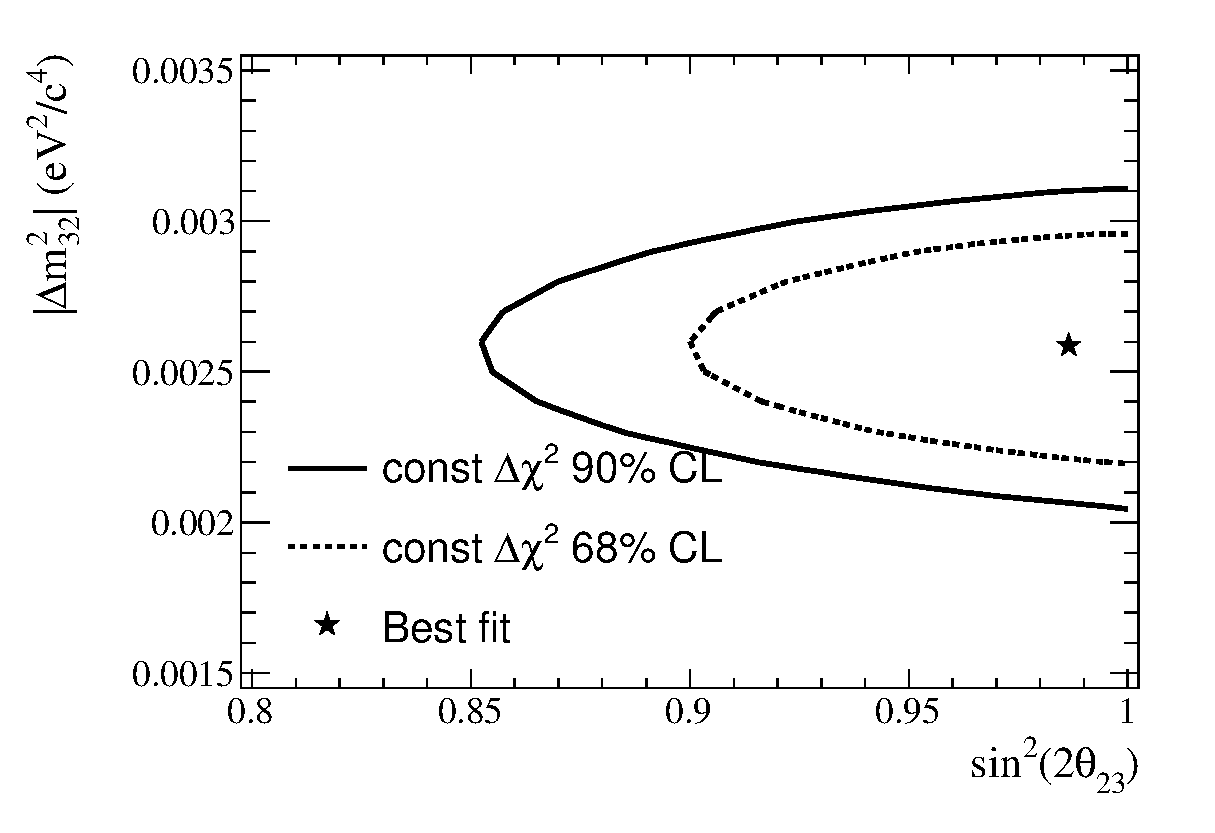
\includegraphics[width=25pc]{./images/fit_data/2N/contours_4}
\caption {
  As in Fig.\ \ref{fig:results_data123_contour_2N}, but for the Run 1+2 dataset only.
}
\label{fig:results_data12_contour_2N}
\end{minipage}
\vfill%\hspace{0.06\linewidth}
\begin{minipage}[t]{0.9\linewidth}
\center
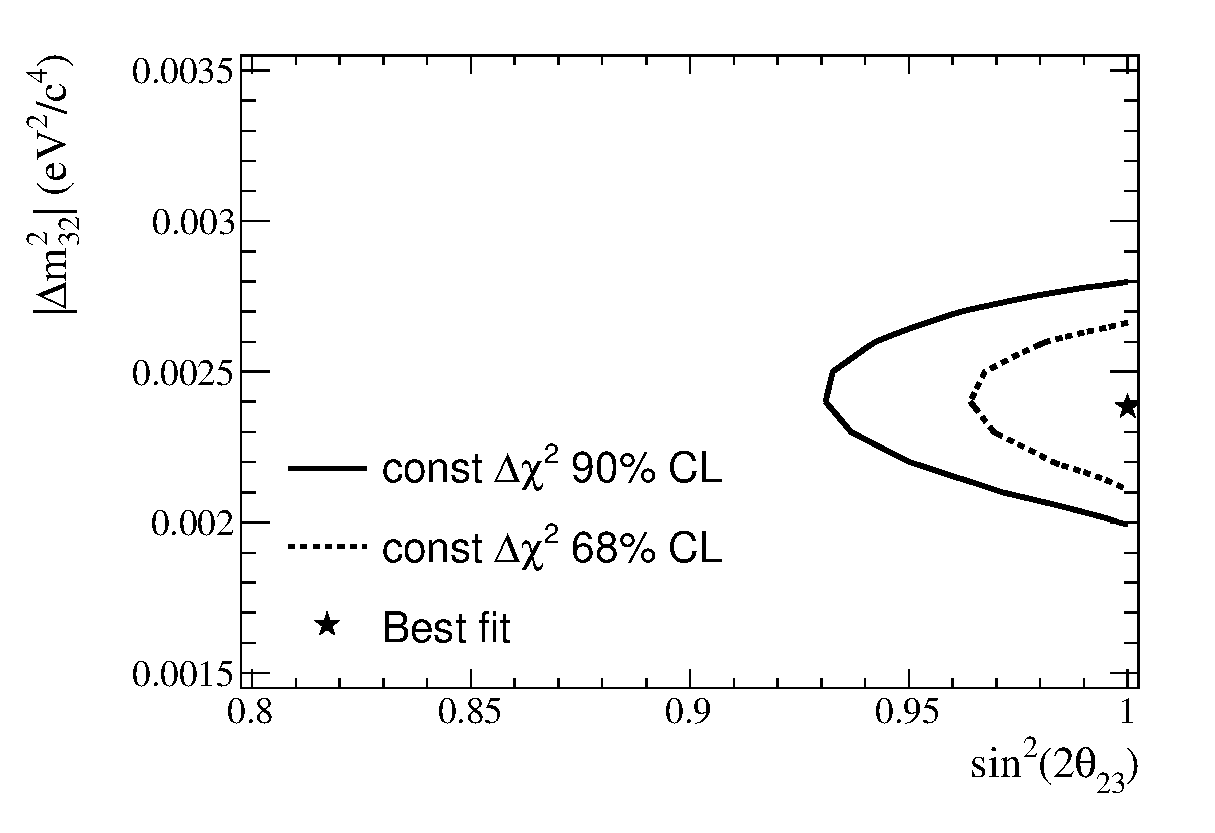
\includegraphics[width=25pc]{./images/fit_data/2N/contours_5}
\caption {
  As in Fig.\ \ref{fig:results_data123_contour_2N}, but for the Run 3 dataset only.
}
\label{fig:results_data3_contour_2N}
\end{minipage}
\end{figure*}


%...........................................................
%
% Const-dchi^2  contours for `2+8' fits
%
\begin{figure*}[htb]
\center
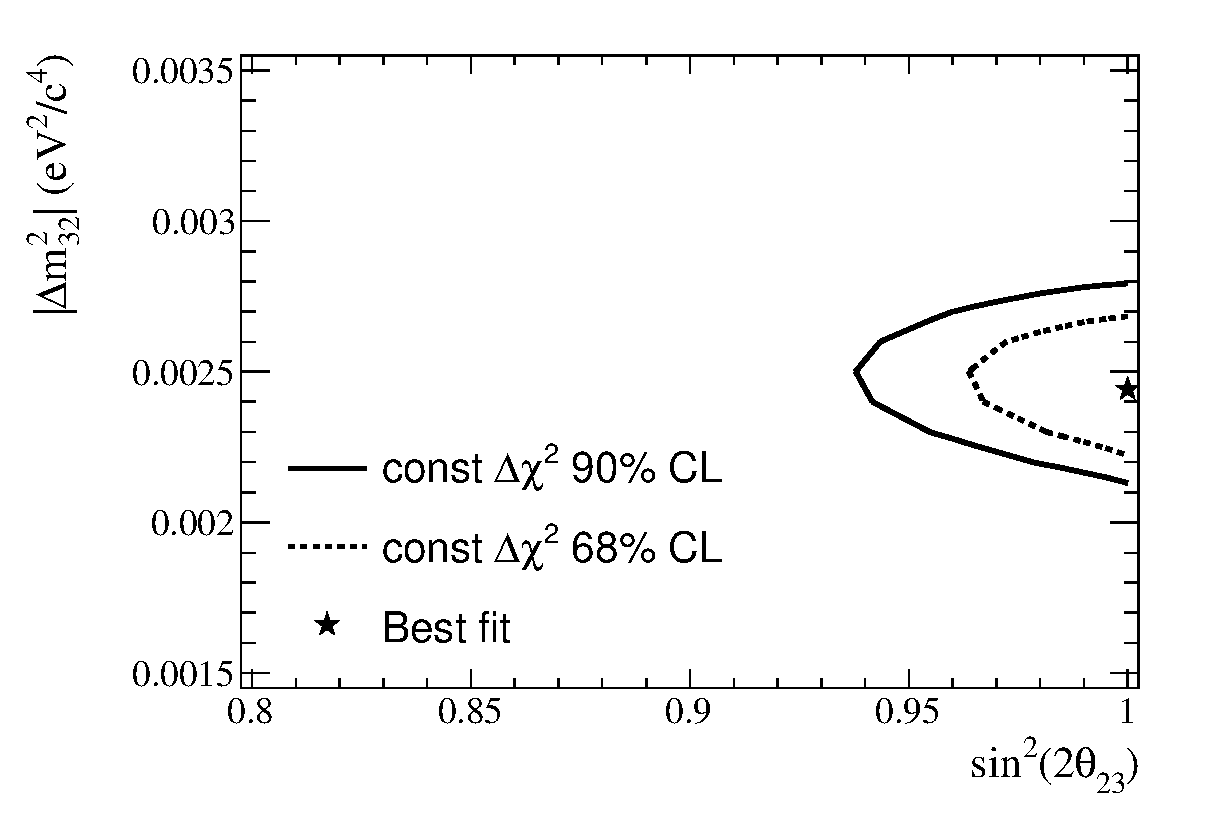
\includegraphics[width=35pc]{./images/fit_data/28/contours_3}
\caption {
  68\% CL and 90\% CL allowed region (including systematics), 
  constructed with the constant-$\Delta\chi^{2}$ method,
  for the `2+8' fit to the Run 1+2+3 dataset.
  The `2+8' best-fit point is also shown.
}
\label{fig:results_data123_contour}
\end{figure*}

\begin{figure*}[htb]
\begin{minipage}[t]{0.48\linewidth}
\center
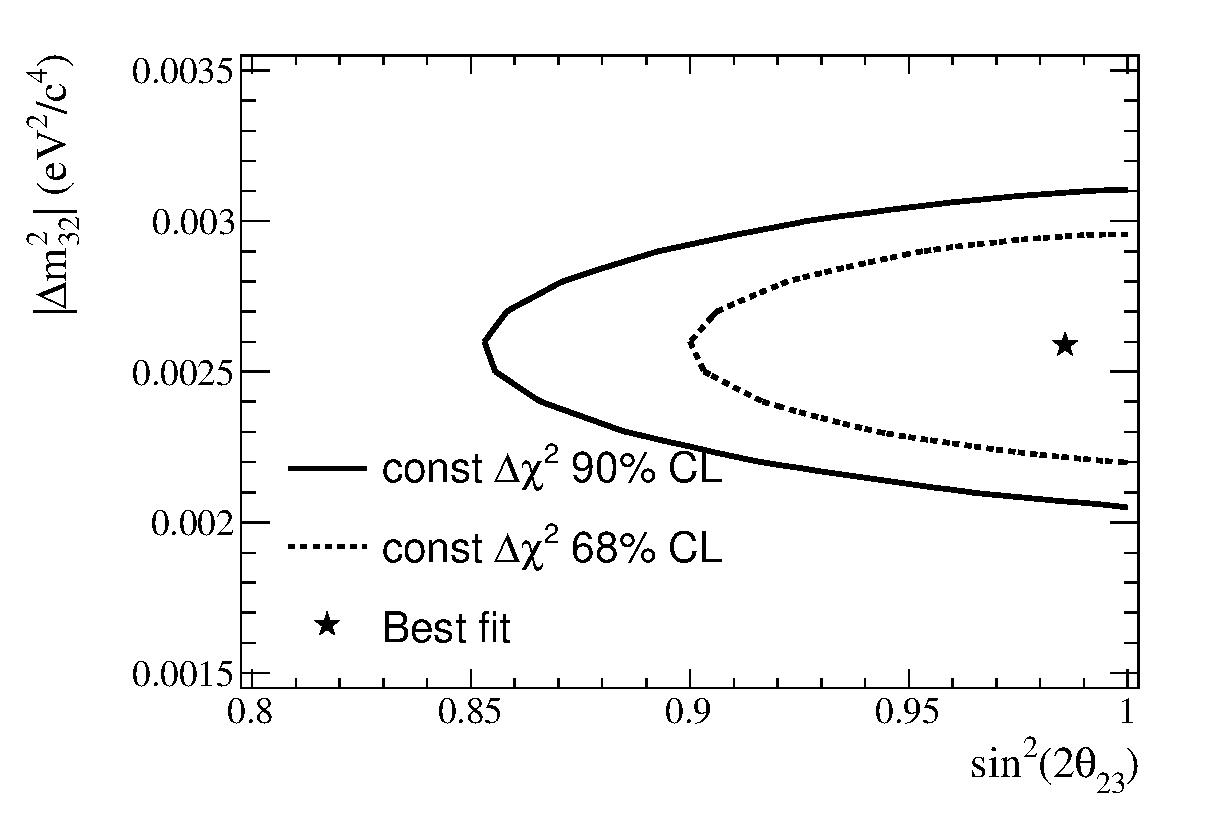
\includegraphics[width=20pc]{./images/fit_data/28/contours_4}
\caption {
  As in Fig.\ \ref{fig:results_data123_contour}, but for the Run 1+2 dataset only.
}
\label{fig:results_data12_contour}
\end{minipage}
\hspace{0.06\linewidth}
\begin{minipage}[t]{0.48\linewidth}
\center
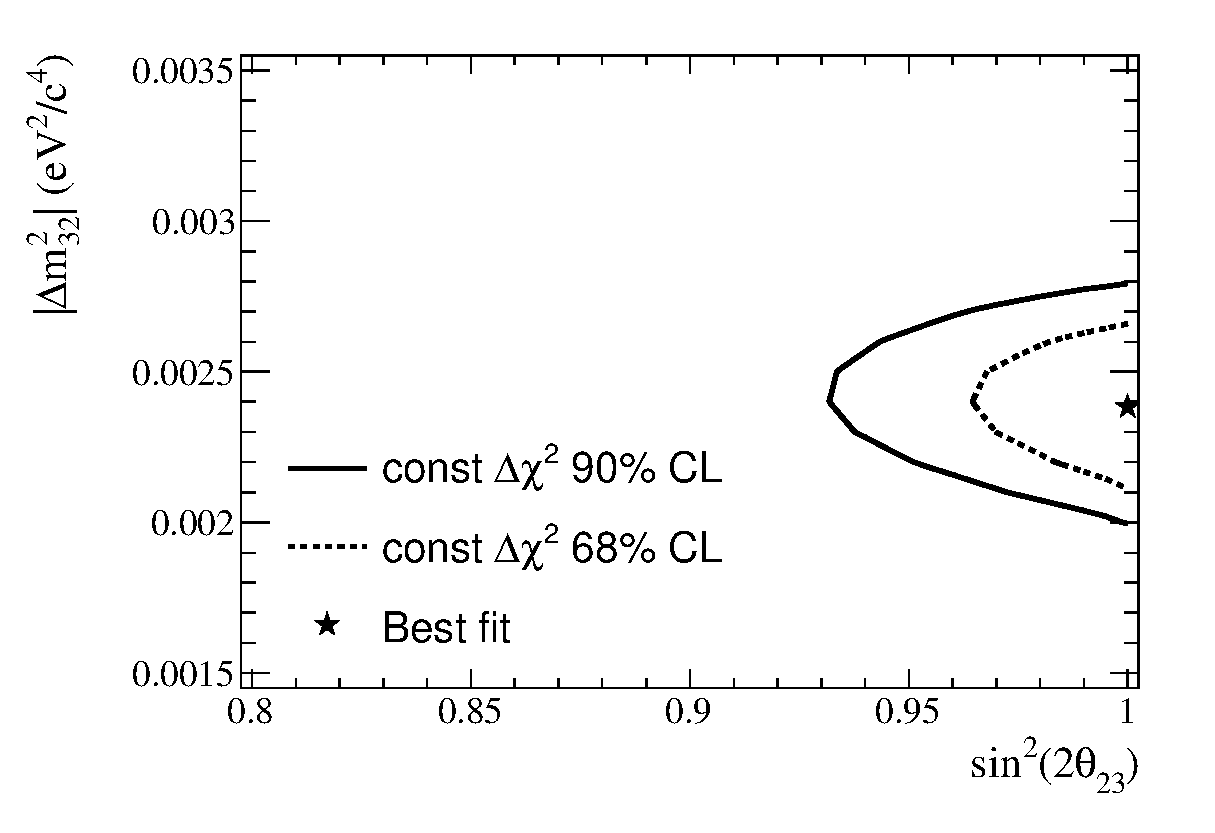
\includegraphics[width=20pc]{./images/fit_data/28/contours_5}
\caption {
  As in Fig.\ \ref{fig:results_data123_contour}, but for the Run 3 dataset only.
}
\label{fig:results_data3_contour}
\end{minipage}
\end{figure*}

%...........................................................
%
% FC contours for `2+N' fits
%

\begin{figure*}[htb]
\center
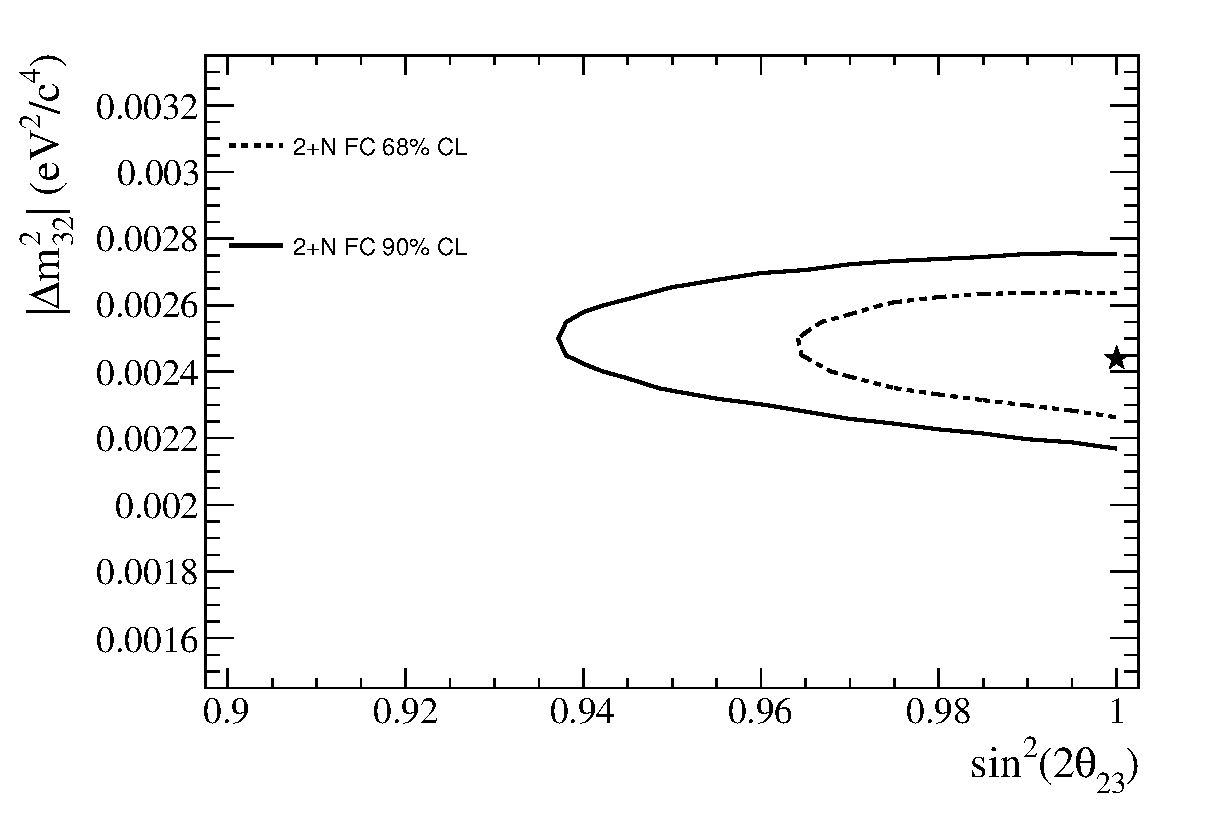
\includegraphics[width=35pc]{./images/fit_data/2N/2N_FC}
\caption {
  68\% CL and 90\% CL allowed region (including systematics), 
  constructed with the method of Feldman and Cousins,
  for the `2+N' fit to the Run 1+2+3 dataset assuming $\theta_{23}$ is in the first octant.
  The `2+N' best-fit point is also shown.
}
\label{fig:results_data123_fc_contour_2N}
\end{figure*}

\begin{figure*}[htb]
\center
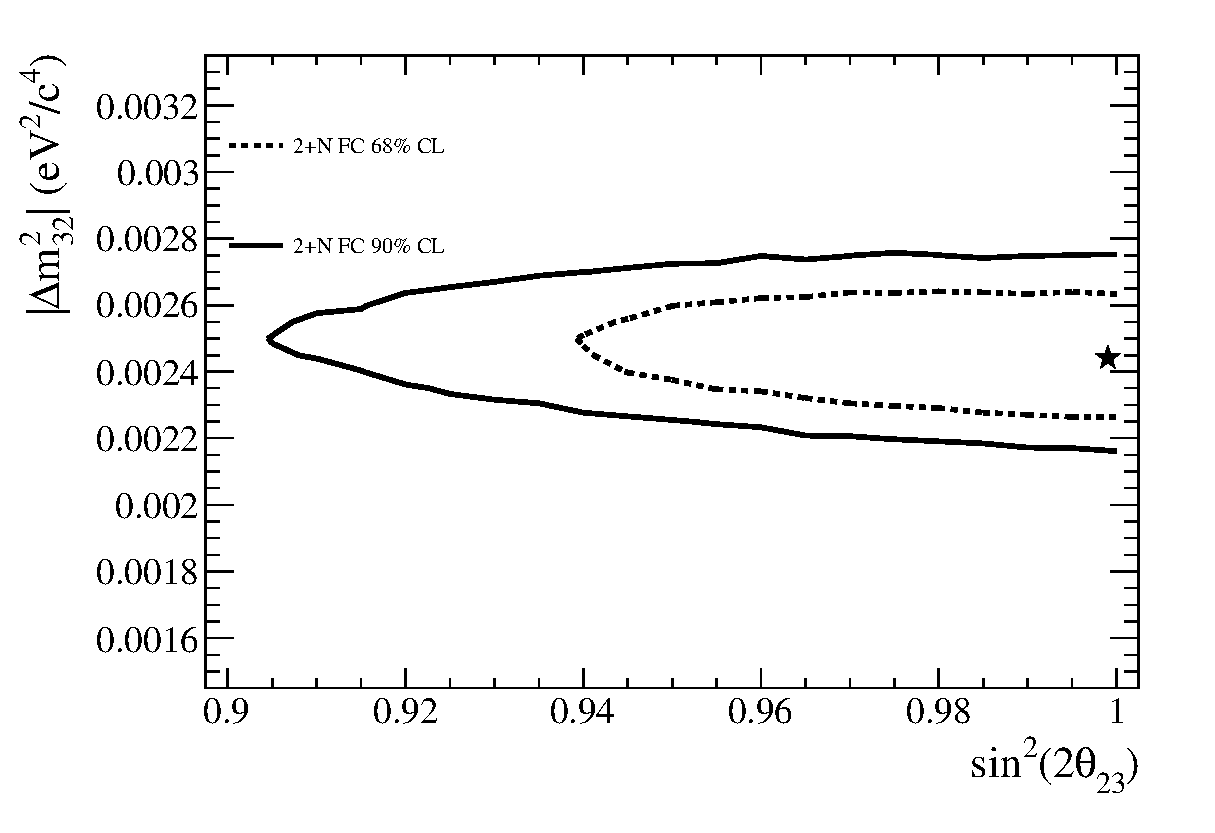
\includegraphics[width=35pc]{./images/fit_data/2Noctant2/2NO2_FC}
\caption {
  68\% CL and 90\% CL allowed region (including systematics), 
  constructed with the method of Feldman and Cousins,
  for the `2+N' fit to the Run 1+2+3 dataset assuming $\theta_{23}$ is in the second octant.
  The `2+N' best-fit point is also shown.
}
\label{fig:results_data123_fc_contour_2NO2}
\end{figure*}

%
%\begin{figure*}[htb]
%\begin{minipage}[t]{0.48\linewidth}
%\center
%
\includegraphics[width=20pc]{./images/placeholder}
%\caption {
%  As in Fig.\ \ref{fig:results_data123_fc_contour_2N}, but for the Run 1+2 dataset only.
%}
%\label{fig:results_data12_fc_contour_2N}
%\end{minipage}
%\hspace{0.06\linewidth}
%\begin{minipage}[t]{0.48\linewidth}
%\center
%
\includegraphics[width=20pc]{./images/placeholder}
%\caption {
%  As in Fig.\ \ref{fig:results_data123_fc_contour_2N}, but for the Run 3 dataset only.
%}
%\label{fig:results_data3_fc_contour_2N}
%\end{minipage}
%\end{figure*}
%

%...........................................................
%
% FC contours for `2+8' fits
%

\begin{figure*}[htb]
\center
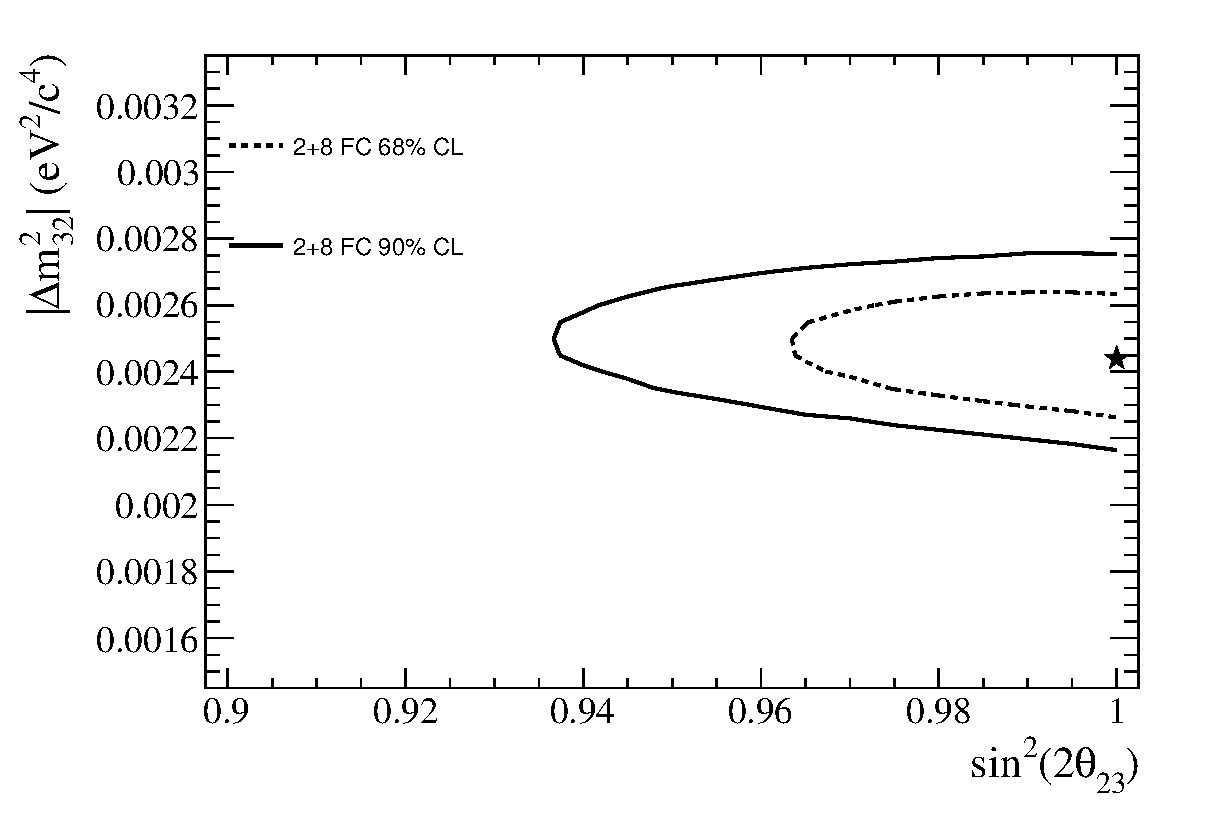
\includegraphics[width=35pc]{./images/fit_data/28/28_FC}
\caption {
  68\% CL and 90\% CL allowed region (including systematics), 
  constructed with the method of Feldman and Cousins,
  for the `2+8' fit to the Run 1+2+3 dataset.
  The `2+8' best-fit point is also shown.
}
\label{fig:results_data123_fc_contour}
\end{figure*}

%
%\begin{figure*}[htb]
%\begin{minipage}[t]{0.48\linewidth}
%\center
%
\includegraphics[width=20pc]{./images/placeholder}
%\caption {
%  As in Fig.\ \ref{fig:results_data123_fc_contour}, but for the Run 1+2 dataset only.
%}
%\label{fig:results_data12_fc_contour}
%\end{minipage}
%\hspace{0.06\linewidth}
%\begin{minipage}[t]{0.48\linewidth}
%\center
%
\includegraphics[width=20pc]{./images/placeholder}
%\caption {
%  As in Fig.\ \ref{fig:results_data123_fc_contour}, but for the Run 3 dataset only.
%}
%\label{fig:results_data3_fc_contour}
%\end{minipage}
%\end{figure*}
%

\clearpage

%--------------------------------------------------------------------------------------
% Contour comparisons
%--------------------------------------------------------------------------------------

\subsection {Confidence region comparisons}
\label{sec:results_contour_comparisons}


\subsubsection {Comparisons between the `2+N' contours assuming $\theta_{23}$ is in the first and second octants}

Comparisons were made between the allowed regions obtained using 
the different fits to the Run 1+2+3 dataset, 
A comparison between $\theta_{23}$ octant assumptions for the `2+N' regions 
constructed using the constant-$\Delta\chi^2$ method
is shown in Fig.\ \ref{fig:results_compare_contours_octants}.
A comparison between $\theta_{23}$ octant assumptions for the `2+N' regions 
constructed using the method of Feldman and Cousins
is shown in Fig.\ \ref{fig:results_compare_fc_contours_octants}.
The contours are visibly different; this is due to the next-to-leading order term in
Eq.\ \ref{eqn:numusurv3fapprox}.

Constant $\Delta\chi^2$ contours for both $\theta_{23}$ octant assumptions are converted
into $\sin^2\theta_{23}$-$|\Delta m^2_{32}|$ space in
Fig.\ \ref{fig:results_compare_contours_octants_sinsqtheta23}.
They are compared with the fit to $\sin^2\theta_{23}$.
% \footnote{
%   A fully validated fit to the Run 1+2+3 dataset using the VaLOR framework for $|\Delta m^2|$, $\sin^2\theta_{23}$ is presented
%   in \cite{OurRun123JointOscillationAnalysis}. The $\nu_\mu$ disappearance result from that note
%   is not shown here, due to that analysis using a different version of the BANFF matrix,
%   however it gives almost identical results.
% }.
The contours are identical, showing that the difference between contours from different $\theta_{23}$ octant
assumptions shown in Fig. \ref{fig:results_compare_contours_octants} is what is expected.
The best-fit values in $\sin^2\theta_{23}$ of the 3 fits are given in Tab.\ \ref{tab:bestfit_sinsqtheta}.

%......................................
% 2+N octants, const Delta\chisq method
%
\begin{figure*}[htb]
\center
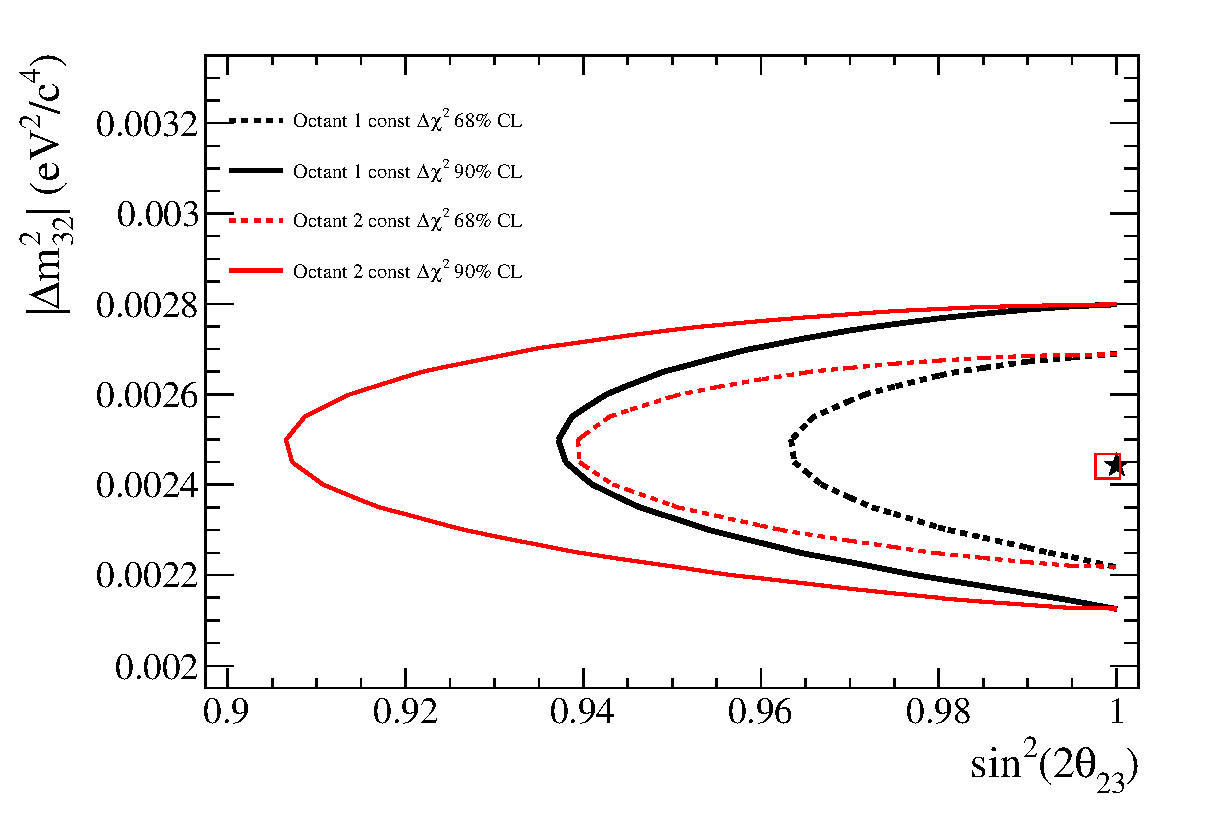
\includegraphics[width=35pc]{./images/fit_data/compare/compare_octants}
\caption {
  Comparison between the `2+N'
  68\% CL and 90\% CL allowed regions
  for $\theta_{23}$ in the first and second octants
  obtained using the constant-$\Delta\chi^2$ method. 
  The comparison is shown for the fits to the Run 1+2+3 dataset.
}
\label{fig:results_compare_contours_octants}
\end{figure*}

%......................................
% 2+N octants, FC method
%
\begin{figure*}[htb]
\center
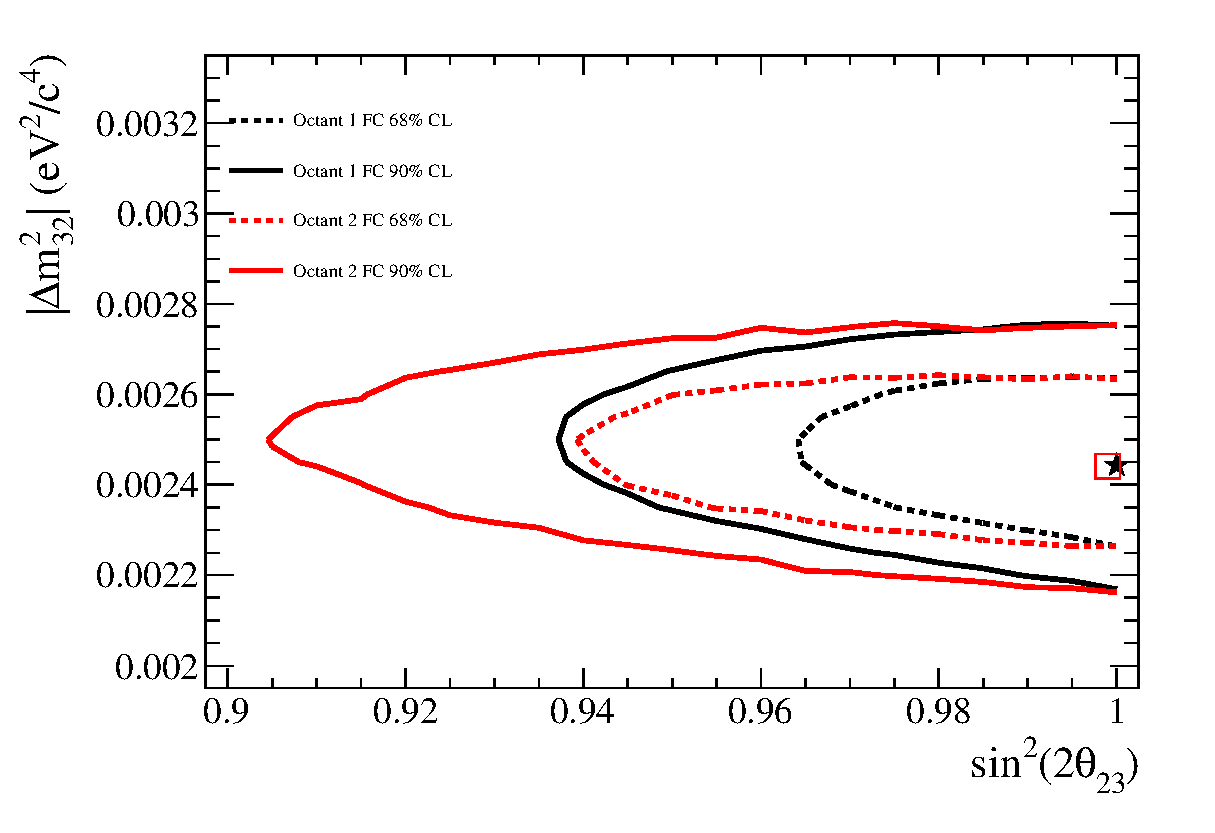
\includegraphics[width=35pc]{./images/fit_data/compare/compare_octants_FC}
\caption {
  Comparison between the `2+N'
  68\% CL and 90\% CL allowed regions
  for $\theta_{23}$ in the first and second octants
  obtained using the method of Feldman and Cousins.
  The comparison is shown for the fits to the Run 1+2+3 dataset.
}
\label{fig:results_compare_fc_contours_octants}
\end{figure*}

%......................................
% 2+N octants, converted into sinsqtheta23 space
%
\begin{figure*}[htb]
\center
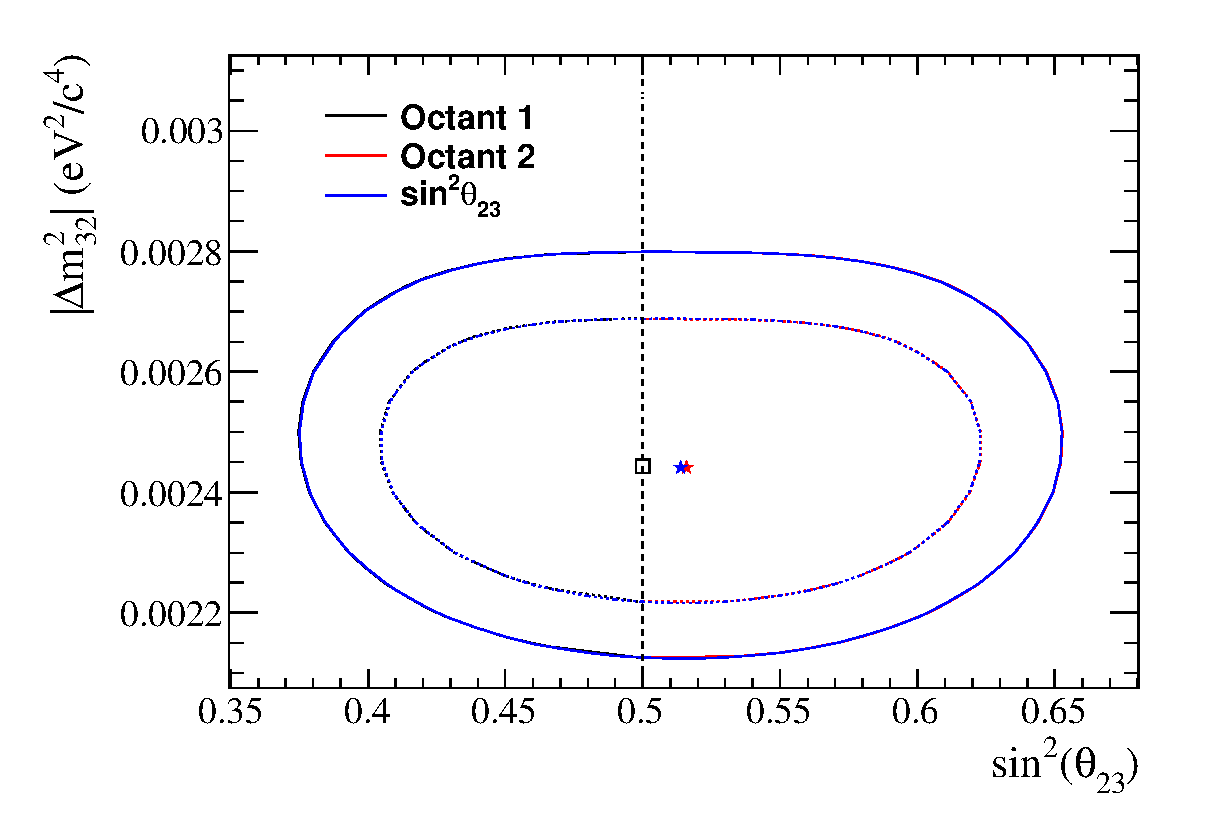
\includegraphics[width=35pc]{./images/fit_data/compare/contour_compare_octants_sinsqtheta}
\caption {
  Comparison between the `2+N'
  68\% CL and 90\% CL allowed regions
  for $\theta_{23}$ in the first and second octants
  obtained using the constant-$\Delta\chi^2$ method,
  and with the x-axis converted from $\sin^2 2 \theta_{23}$ to $\sin^2\theta_{23}$ after the fit.
  A '2+N' fit using $\sin^2\theta_{23}$ directly is also shown.
  The vertical line is the boundary between the octants to help guide the
  reader's eye.
  The comparison is shown for the fits to the Run 1+2+3 dataset.
}
\label{fig:results_compare_contours_octants_sinsqtheta23}
\end{figure*}

\clearpage

\subsubsection {Comparisons between the `2+N' and `2+8' contours}

Comparisons were made between the allowed regions obtained using 
the different fits to the Run 1+2+3 dataset, 
A comparison between the `2+N' and `2+8' regions 
constructed using the constant-$\Delta\chi^2$ method
is shown in Fig.\ \ref{fig:results_compare_contours_28_2N}.
A comparison between the `2+N' and `2+8' regions
constructed using the method of Feldman and Cousins
is shown in Fig.\ \ref{fig:results_compare_fc_contours_28_2N}.
For a given contour construction method,
the `2+N' and `2+8' contours are almost identical.

Fig.\ \ref{fig:results_compare_contours_28_2N_20} shows a comparison
between the `2+N' and `2+8' regions, constructed using the 
constant-$\Delta\chi^2$ method, with the corresponding results for `2+0'.
The `2+0' fit results in smaller contours.
The plot illustrates that, while with the present statistics fitting for 
systematics is warranted (`2+0' contours smaller than `2+8' and `2+N'),
the full effect of the systematics on the contour is encapsulated
by allowing only the the 8 dominant to float in the fit.

%......................................
% 2+N vs 2+8, const Delta\chisq method
%
\begin{figure*}[htb]
\center
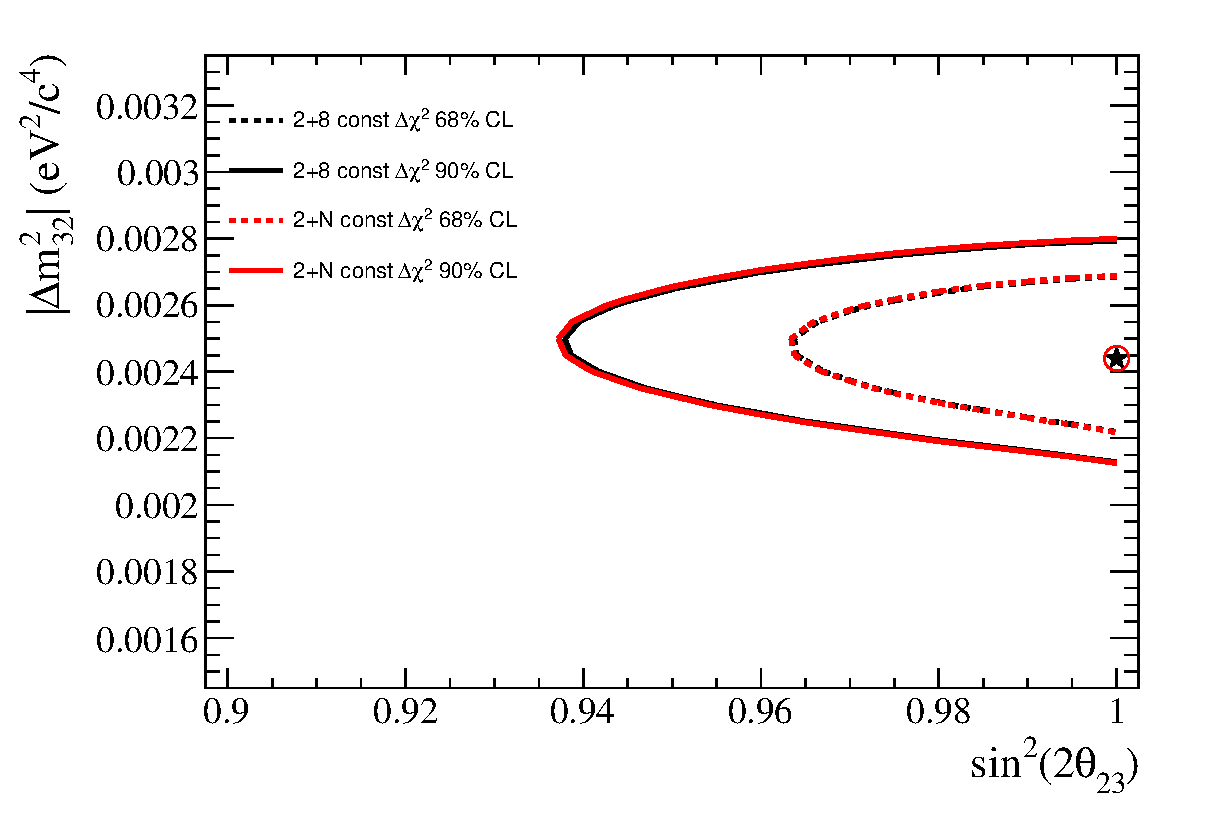
\includegraphics[width=35pc]{./images/fit_data/compare/compare_2all_28}
\caption {
  Comparison between the `2+N' and `2+8'
  68\% CL and 90\% CL allowed regions 
  obtained using the constant-$\Delta\chi^2$ method. 
  The comparison is shown for the fits to the Run 1+2+3 dataset.
  The `2+N' and `2+8' confidence regions are identical.
}
\label{fig:results_compare_contours_28_2N}
\end{figure*}

%......................................
% 2+N vs 2+8, FC method
%
\begin{figure*}[htb]
\center
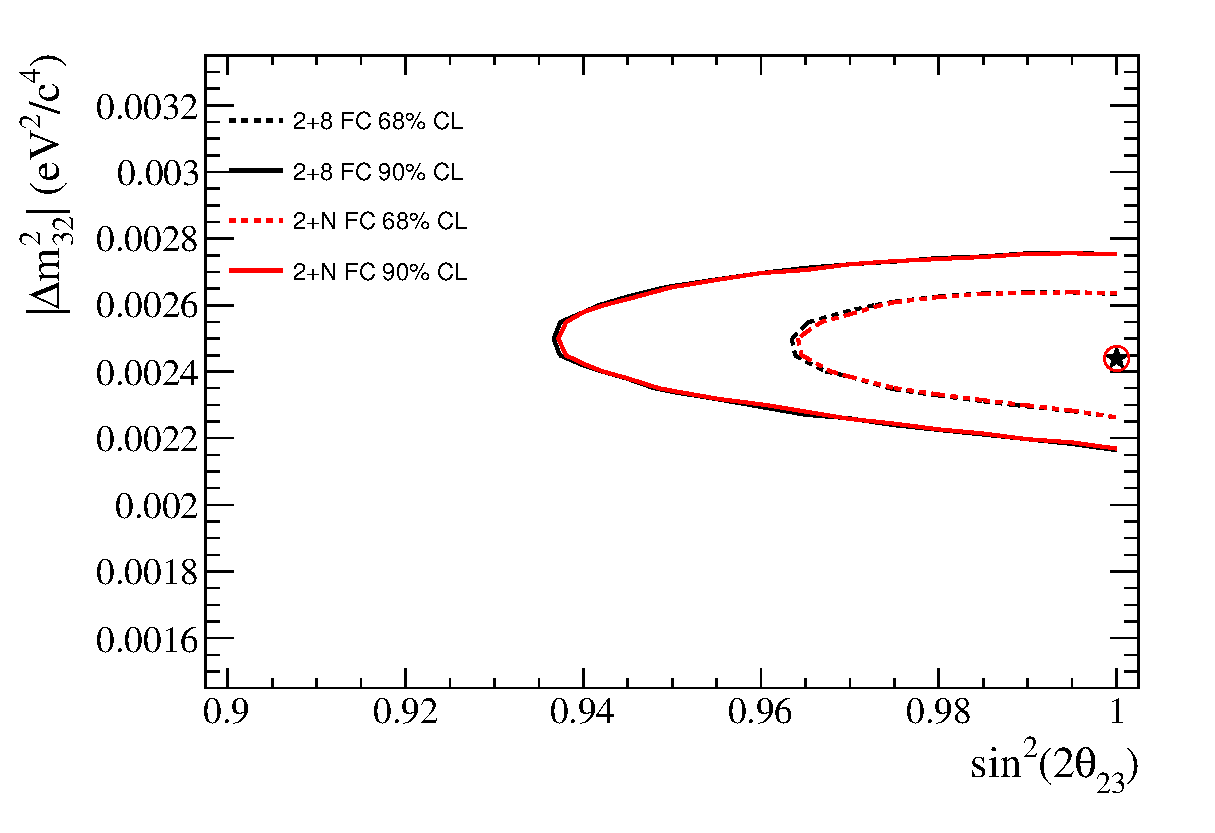
\includegraphics[width=35pc]{./images/fit_data/compare/compare_2all_28_FC}
\caption {
  Comparison between the `2+N' and `2+8'
  68\% CL and 90\% CL allowed regions
  obtained using the method of Feldman and Cousins.
  The comparison is shown for the fits to the Run 1+2+3 dataset.
}
\label{fig:results_compare_fc_contours_28_2N}
\end{figure*}

%......................................
% 2+N vs 2+8 vs 2+0, const Delta\chisq method
%
\begin{figure*}[htb]
\center
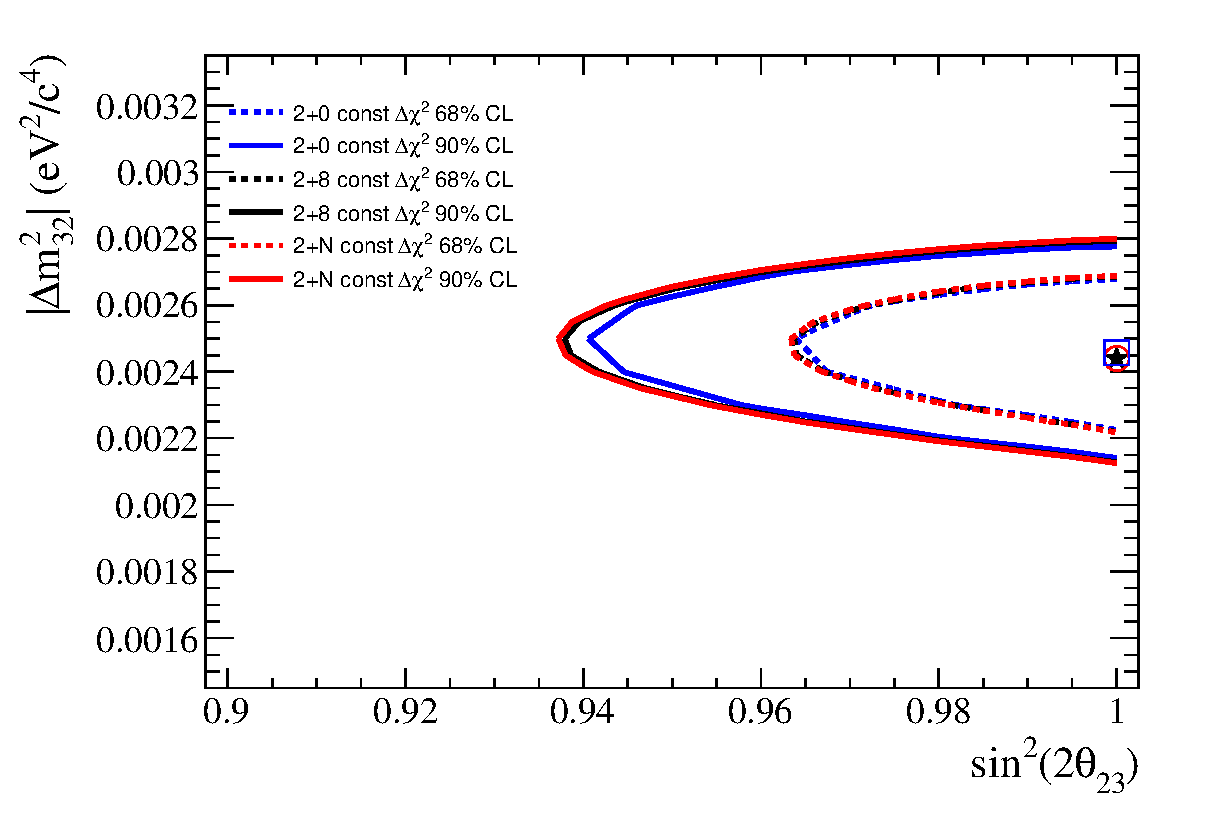
\includegraphics[width=35pc]{./images/fit_data/compare/compare_2all_28_20}
\caption {
  Comparison between the `2+N', `2+8' and `2+0'
  68\% CL and 90\% CL allowed regions 
  obtained using the constant-$\Delta\chi^2$ method. 
  The comparison is shown for the fits to the Run 1+2+3 dataset.
}
\label{fig:results_compare_contours_28_2N_20}
\end{figure*}

\clearpage

%......................................................................................
\subsubsection {Comparisons between the constant-$\Delta\chi^{2}$ and Feldman-Cousins contours}

The confidence regions obtained using the same fit variant 
but different contour construction methods were also compared.
In Fig.\ \ref{fig:results_compare_FC_constdchisq_2N}, 
a comparison between the contours obtained using the constant-$\Delta\chi^2$ and Feldman-Cousins methods
is shown for the `2+N' fit to the Run 1+2+3 dataset.
In Fig.\ \ref{fig:results_compare_FC_constdchisq_2NO2}, 
the same comparison is shown for the `2+N' fit assuming $\theta_{23}$ is in the second octant.
In Fig.\ \ref{fig:results_compare_FC_constdchisq}, 
the same comparison is shown for the `2+8' fit.

%......................
%
% const Delta\chisq vs FC, 2+N
%
\begin{figure*}[htb]
\center
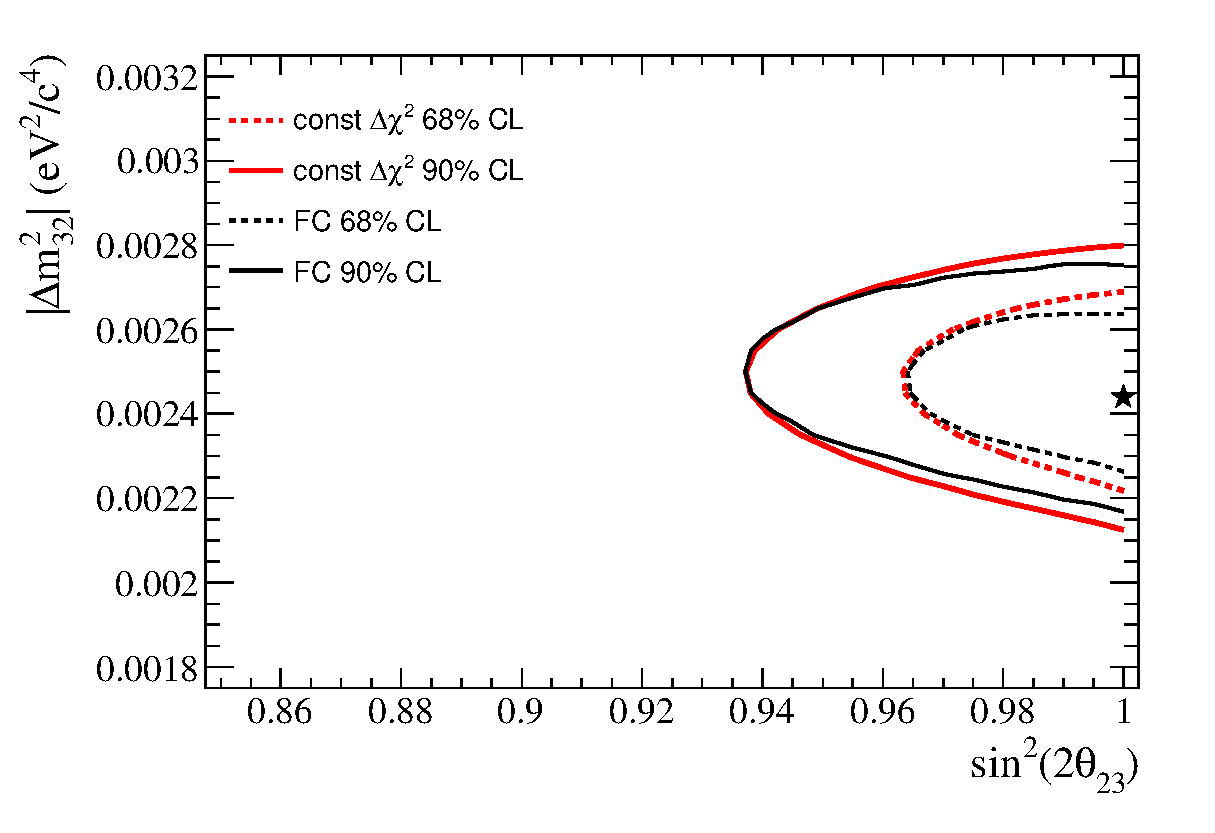
\includegraphics[width=30pc]{./images/fit_data/compare/compare_FC_constchisq_2N}
\caption {
  Comparison between the 68\% CL and 90\% CL allowed regions 
  obtained using the constant-$\Delta\chi^2$ and Feldman-Cousins methods 
  for the `2+N' fit to the Run 1+2+3 dataset assuming $\theta_{23}$ is in the first octant.
}
\label{fig:results_compare_FC_constdchisq_2N}
\end{figure*}


%......................
%
% const Delta\chisq vs FC, 2+N, second octant
%
\begin{figure*}[htb]
\center
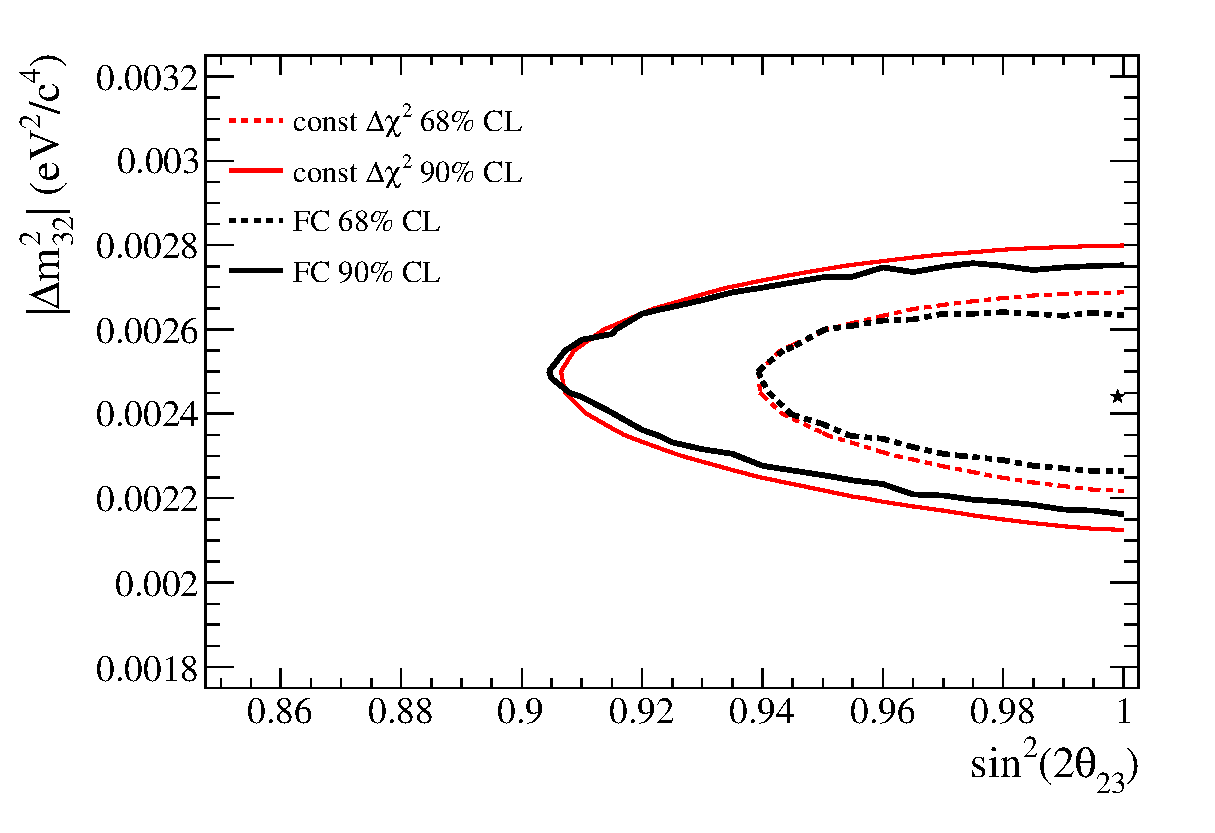
\includegraphics[width=30pc]{./images/fit_data/compare/compare_FC_constchisq_2NO2}
\caption {
  Comparison between the 68\% CL and 90\% CL allowed regions 
  obtained using the constant-$\Delta\chi^2$ and Feldman-Cousins methods 
  for the `2+N' fit to the Run 1+2+3 dataset assuming $\theta_{23}$ is in the second octant.
}
\label{fig:results_compare_FC_constdchisq_2NO2}
\end{figure*}


%......................
%
% const Delta\chisq vs FC, 2+8
%
\begin{figure*}[htb]
\center
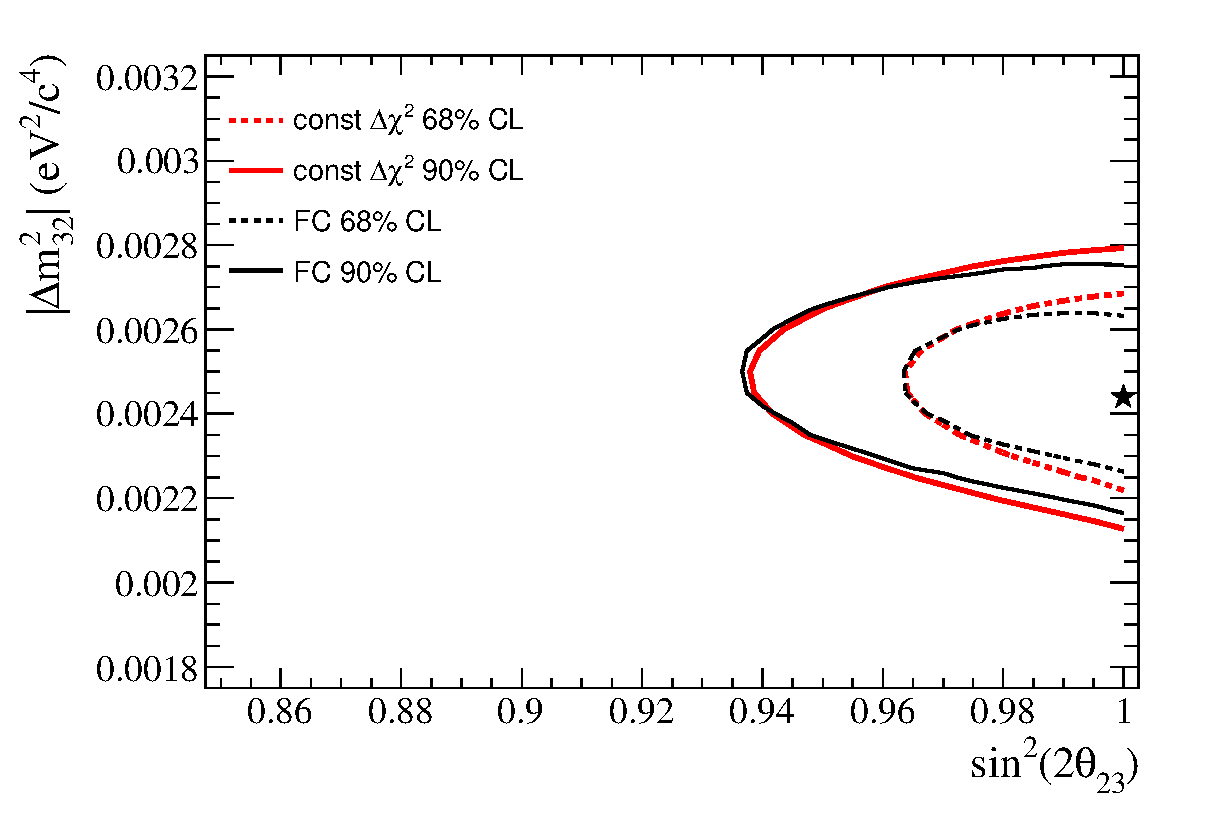
\includegraphics[width=30pc]{./images/fit_data/compare/compare_FC_constchisq}
\caption {
  Comparison between the 68\% CL and 90\% CL allowed regions 
  obtained using the constant-$\Delta\chi^2$ and Feldman-Cousins methods 
  for the `2+8' fit to the Run 1+2+3 dataset.
}
\label{fig:results_compare_FC_constdchisq}
\end{figure*}

\clearpage

%......................................................................................
\subsubsection {Comparisons with recent measurements from MINOS and SuperK}

Comparisons were produced between our Run 1+2+3 results and the updated results from 
MINOS 2013 (3-flavour analysis) \cite{MINOS2013:3nu} and SuperK 2012 atmospherics (3-flavour 
zenith-angle analysis) \cite{SKAtm2012}.
The comparison is shown 
in Fig.\ \ref{fig:results_compare_FC_constdchisq_external_2Nsintheta} for the `2+N' fit for $\sin^2\theta_{23}$.

Comparisons were produced between our Run 1+2+3 results and the updated (2012) results from 
MINOS \cite{MINOS2012} and SuperK atmospherics (both the 2-flavour L/E and 3-flavour 
zenith-angle analyses) \cite{SKAtm2012}.
The comparison is shown 
in Fig.\ \ref{fig:results_compare_FC_constdchisq_external_2N} for the `2+N' fit assuming $\theta_{23}$ is in the first octant,
in Fig.\ \ref{fig:results_compare_FC_constdchisq_external_2NO2} for the `2+N' fit assuming it is in the second octant, and
in Fig.\ \ref{fig:results_compare_FC_constdchisq_external} for the `2+8' fit.
A comparison of '2+N' FC contours with the external data is shown in Fig.\ \ref{fig:results_compare_FC_octants}
for both octant assumptions.

%......................
%
% VaLOR vs the world, 2+N sintheta
%
\begin{figure*}[htb]
\center
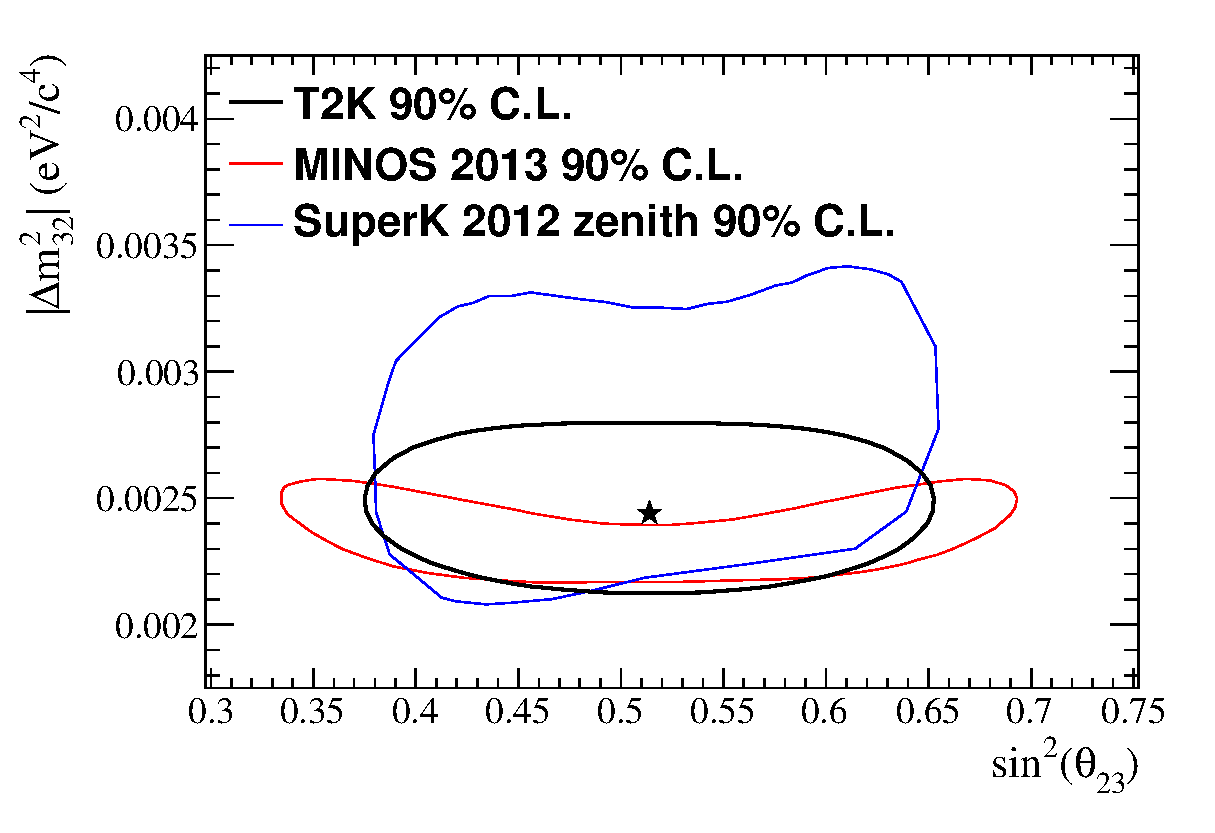
\includegraphics[width=30pc]{./images/fit_data/compare/compare_contours_external_sintheta}
\caption {
  Comparison between 90\% CL allowed regions 
  from MINOS \cite{MINOS2013:3nu} and SuperK atmospherics \cite{SKAtm2012},
  and the 90\% CL region obtained from the VaLOR `2+N' $\sin^2\theta_{23}$ fit to the Run 1+2+3 dataset,
  using the constant-$\Delta\chi^2$ method.
}
\label{fig:results_compare_FC_constdchisq_external_2Nsintheta}
\end{figure*}

%......................
%
% VaLOR vs the world, 2+N
%
\begin{figure*}[htb]
\center
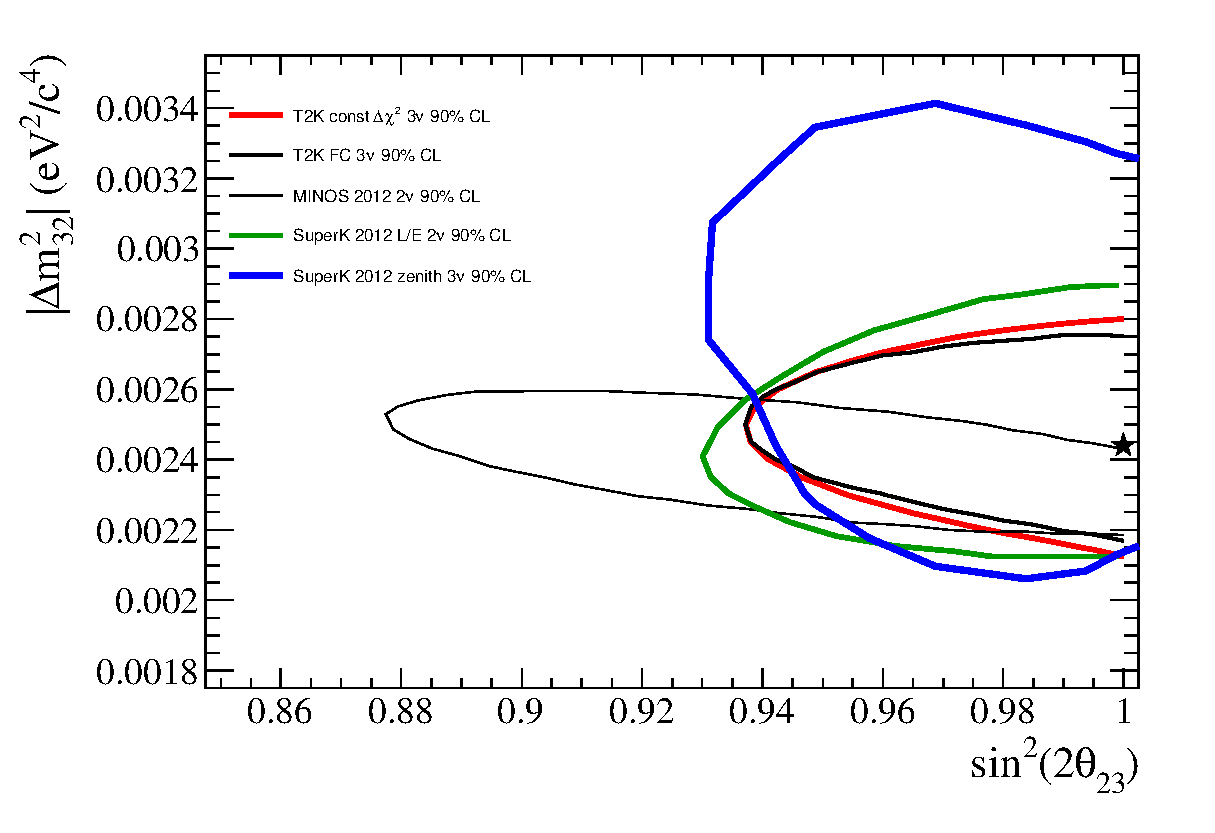
\includegraphics[width=30pc]{./images/fit_data/compare/compare_FC_constchisq_external_2N}
\caption {
  Comparison between 90\% CL allowed regions 
  from MINOS \cite{MINOS2012} and SuperK atmospherics \cite{SKAtm2012},
  and the 90\% CL regions obtained from the VaLOR `2+N' fit to the Run 1+2+3 dataset.
  Contours obtained using both the constant-$\Delta\chi^2$ and Feldman-Cousins methods are shown.
}
\label{fig:results_compare_FC_constdchisq_external_2N}
\end{figure*}

%......................
%
% VaLOR vs the world, 2+N, second octant
%
\begin{figure*}[htb]
\center
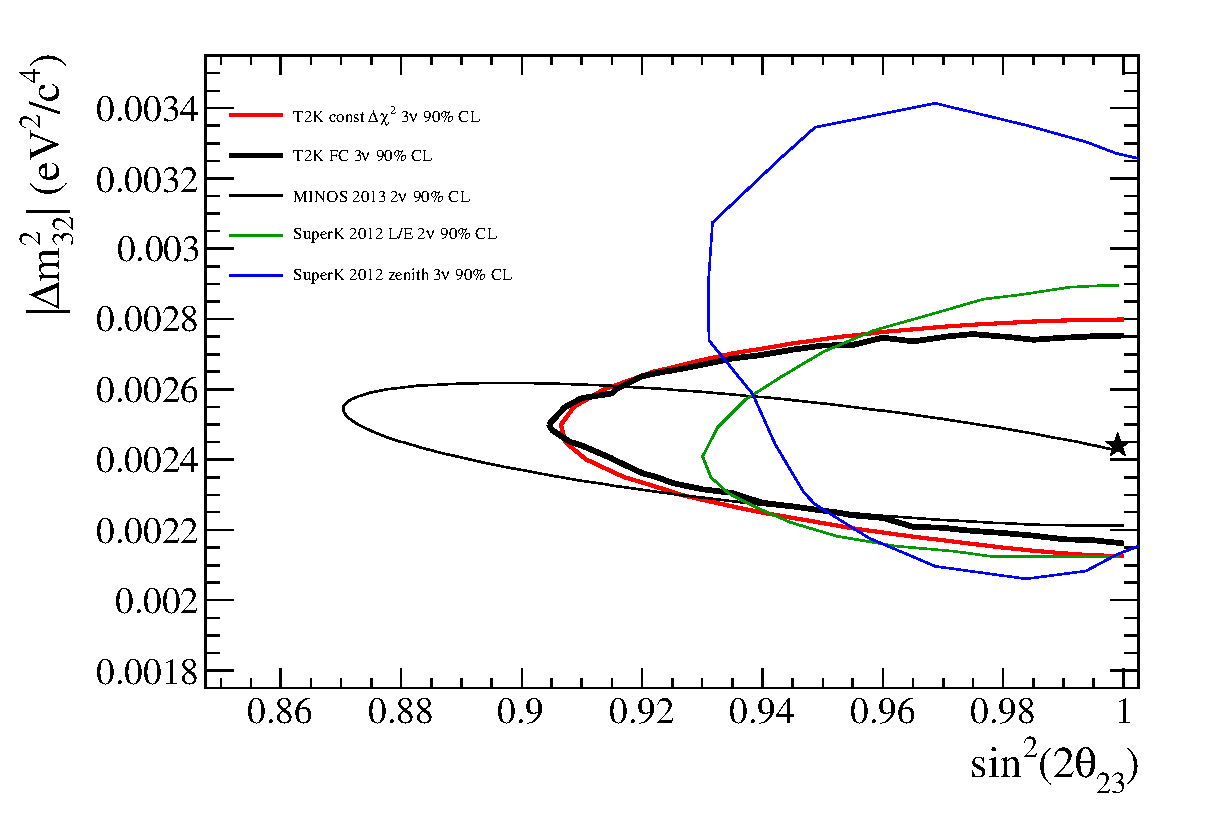
\includegraphics[width=30pc]{./images/fit_data/compare/compare_FC_constchisq_external_2NO2}
\caption {
  As in Fig.\ \ref{fig:results_compare_FC_constdchisq_external_2N}, but for the `2+N' fit assuming $\theta_{23}$ is in the second octant.
}
\label{fig:results_compare_FC_constdchisq_external_2NO2}
\end{figure*}

%......................
%
% VaLOR vs the world, 2+8
%
\begin{figure*}[htb]
\center
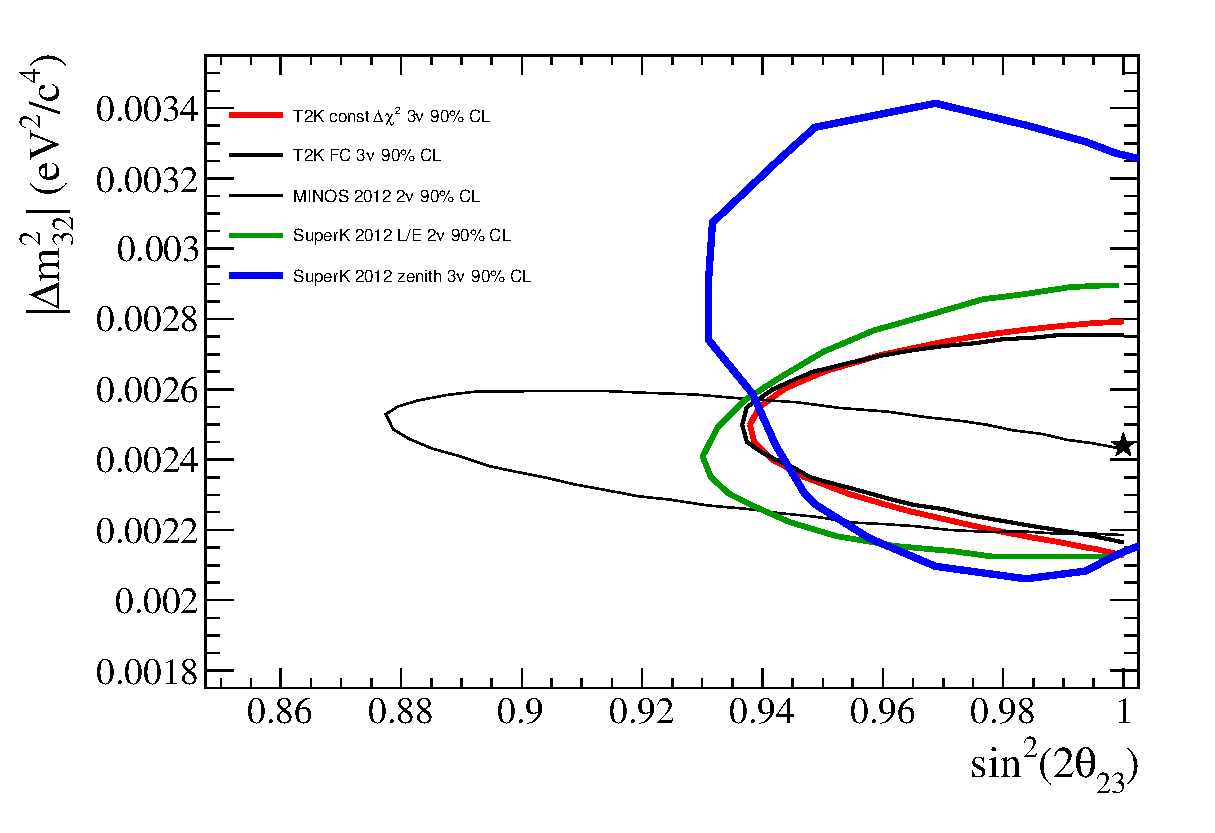
\includegraphics[width=30pc]{./images/fit_data/compare/compare_FC_constchisq_external}
\caption {
  As in Fig.\ \ref{fig:results_compare_FC_constdchisq_external_2N}, but for the `2+8' fit.
}
\label{fig:results_compare_FC_constdchisq_external}
\end{figure*}

%......................
%
% VaLOR vs the world, 2+N, FC, both octants
%
\begin{figure*}[htb]
\center
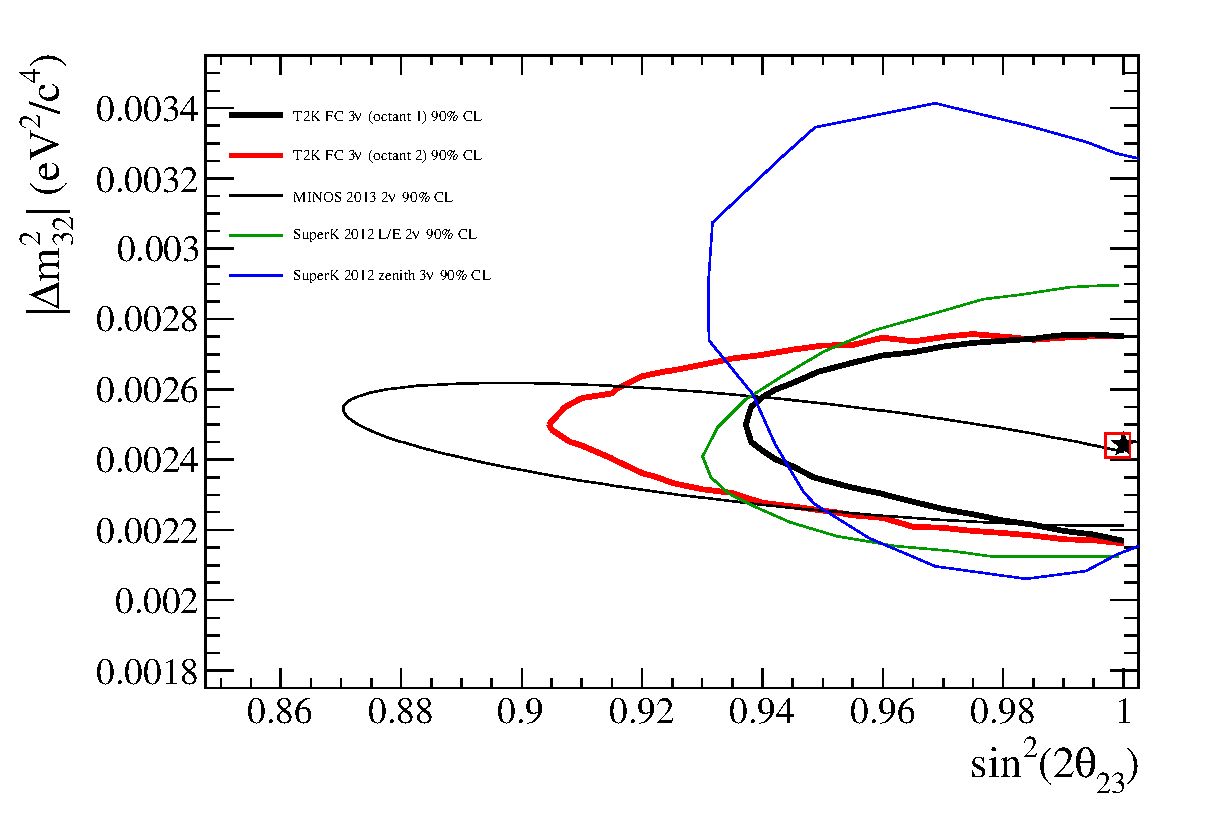
\includegraphics[width=30pc]{./images/fit_data/compare/compare_FC_octants_external}
\caption {
  Comparison between 90\% CL allowed regions 
  from MINOS \cite{MINOS2012} and SuperK atmospherics \cite{SKAtm2012},
  and the 90\% CL regions obtained from the VaLOR `2+N' fit to the Run 1+2+3 dataset.
  Contours obtained using both $\theta_{23}$ octant assumptions are shown.
}
\label{fig:results_compare_FC_octants}
\end{figure*}


\clearpage

%......................................................................................
\subsubsection {Comparisons with sensitivity}

In Fig.\ \ref{fig:results_compare_28_constdchisq_sensitivity}, 
a comparison is shown
between the Run 1+2+3 allowed regions obtained using the `2+8' fit and the
constant-$\Delta\chi^{2}$ method, and the T2K 3.010$\times$10$^{20}$ POT sensitivity
contours produced at the `2+8' best-fit point for the Run 1+2+3 dataset.
The sensitivity contours were computed by averaging the contours of 1k toy-MC
experiments generated with statistical fluctations and all systematic parameters randomized.
The plot indicates that the Run 1+2+3 dataset, is a ``favourable'' fluctuation
allowing us to quote confidence regions which are more restrictive than 
those that would be expected given our sensitivity.
This favourable fluctuation is not unlikely as shown 
in Fig.\ \ref{fig:results_compare_28_constdchisq_sensitivity_exclusion}.

%......................
%
\begin{figure*}[htb]
\center
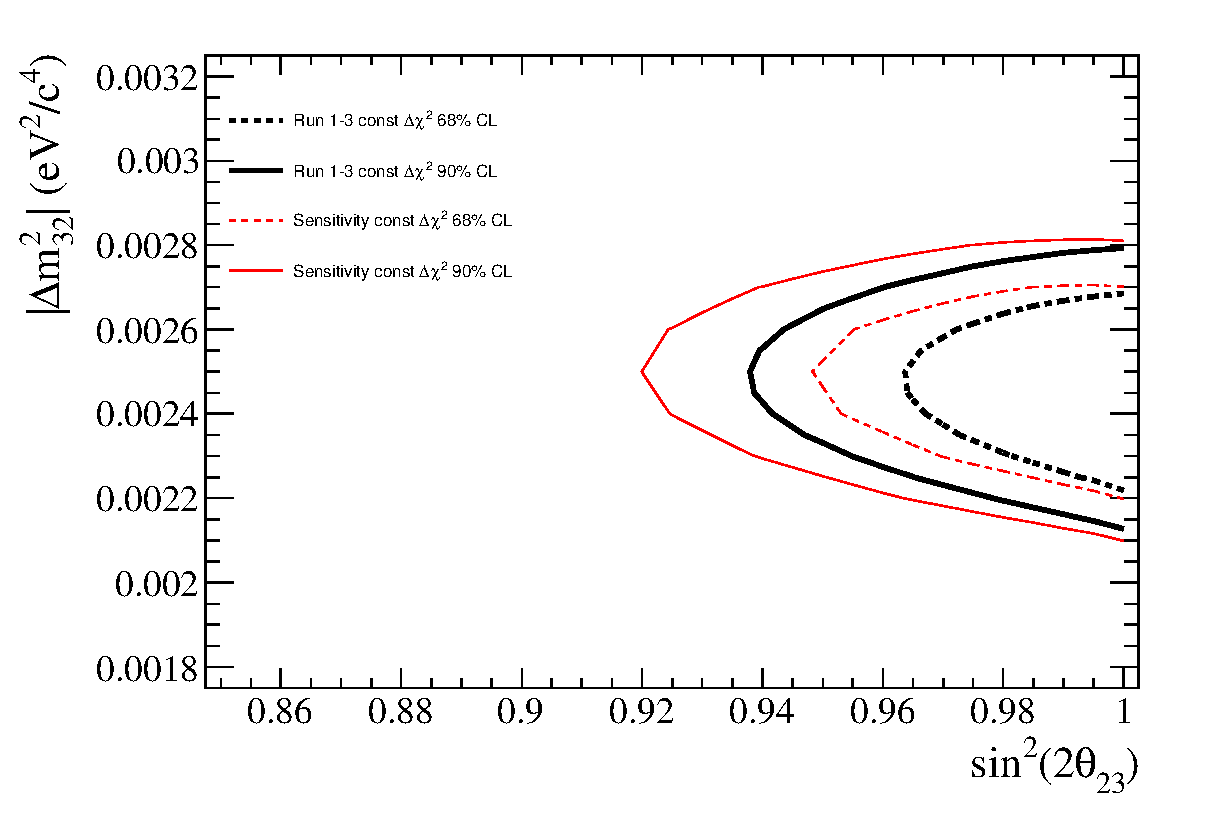
\includegraphics[width=30pc]{./images/fit_data/compare/compare_constchisq_sensitivity}
\caption {
  Comparison between the 68\% CL and 90\% CL allowed regions using the constant-$\Delta\chi^2$ 
  method for the `2+8' fit to the Run 1+2+3 dataset
  and the result of a sensitivity study at the `2+8' best-fit point for Run 1+2+3.
}
\label{fig:results_compare_28_constdchisq_sensitivity}
\end{figure*}

%......................
%
\begin{figure*}[htb]
\center
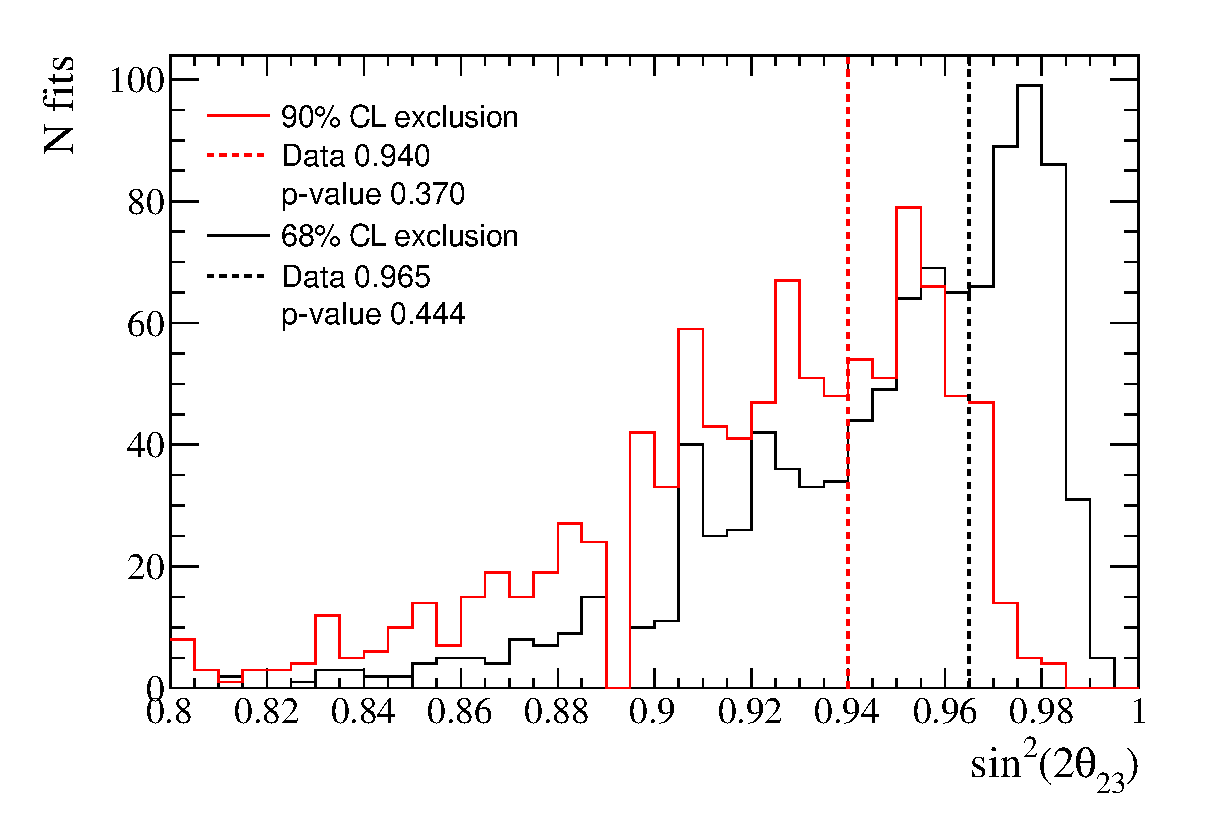
\includegraphics[width=25pc]{./images/sensitivities/2+8constdchisq/sensitivity_exclusion}
\caption {
  Distribution of minimum excluded value of sin$^22\theta_{23}$, for both 68\% CL and 90\% CL.
  The dashed lines show the minimum excluded value for the `2+8' fit
  to the Run 1+2+3 dataset, using the constant-$\Delta \chi^2$ method  
  (68\% CL in black and 90\% CL in red).  
}
\label{fig:results_compare_28_constdchisq_sensitivity_exclusion}
\end{figure*}


\clearpage

%......................................................................................
%\subsubsection {Comparison between the 2012 and 2010 analyses}
%
%Fig. \ref{fig:results_compare_2010_2012}
%
%The
%%......................
%%
%\begin{figure*}[htb]
%\center
%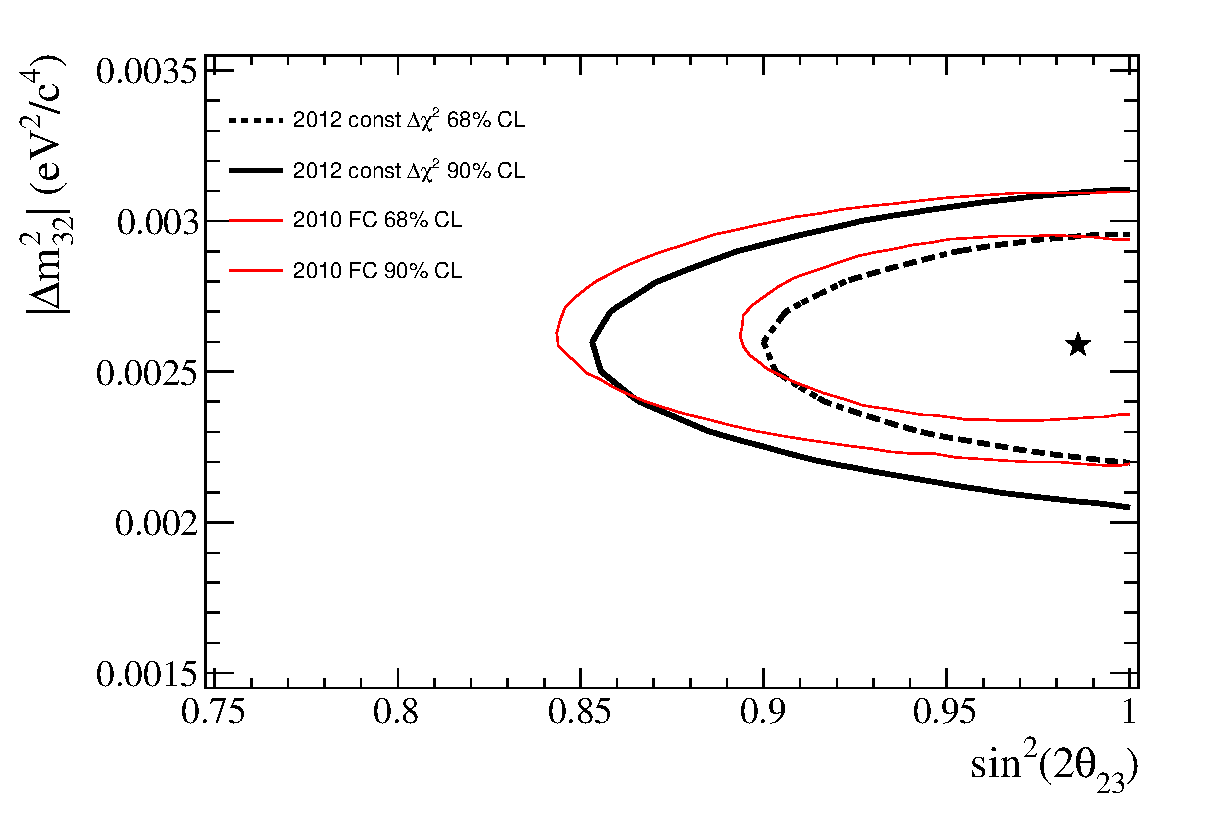
\includegraphics[width=35pc]{./images/fit_data/compare/compare_run12_2012_2010}
%\caption {
%  Comparison of 68\% CL and 90\% CL allowed regions of 2010 and 2012 methods, in a fit to Run I+II data.
%  The 2012 result shown used the 2+8 constant-$\Delta\chi^2$ method.
%  The 2010 result is taken from \cite{OurRun12DisappAnalysis}.
%}
%\label{fig:results_compare_2010_2012}
%\end{figure*}
%
%
%......................................................................................

\subsubsection {Comparisons of individual run periods}

A comparison between the confidence regions obtained by three 
separate `2+N' analyses of the Run 1+2+3, Run 1+2 and Run 3 datasets 
is shown in Fig.\ \ref{fig:results_compare_runs_2N}.
The corresponding plot for the `2+8' fit  
is shown in Fig.\ \ref{fig:results_compare_runs}.
The contours from the different running periods are consistent.

%......................
%
% Run1+2+3 vs Run1+2 vs Run3, 2+N
%
\begin{figure*}[htb]
\center
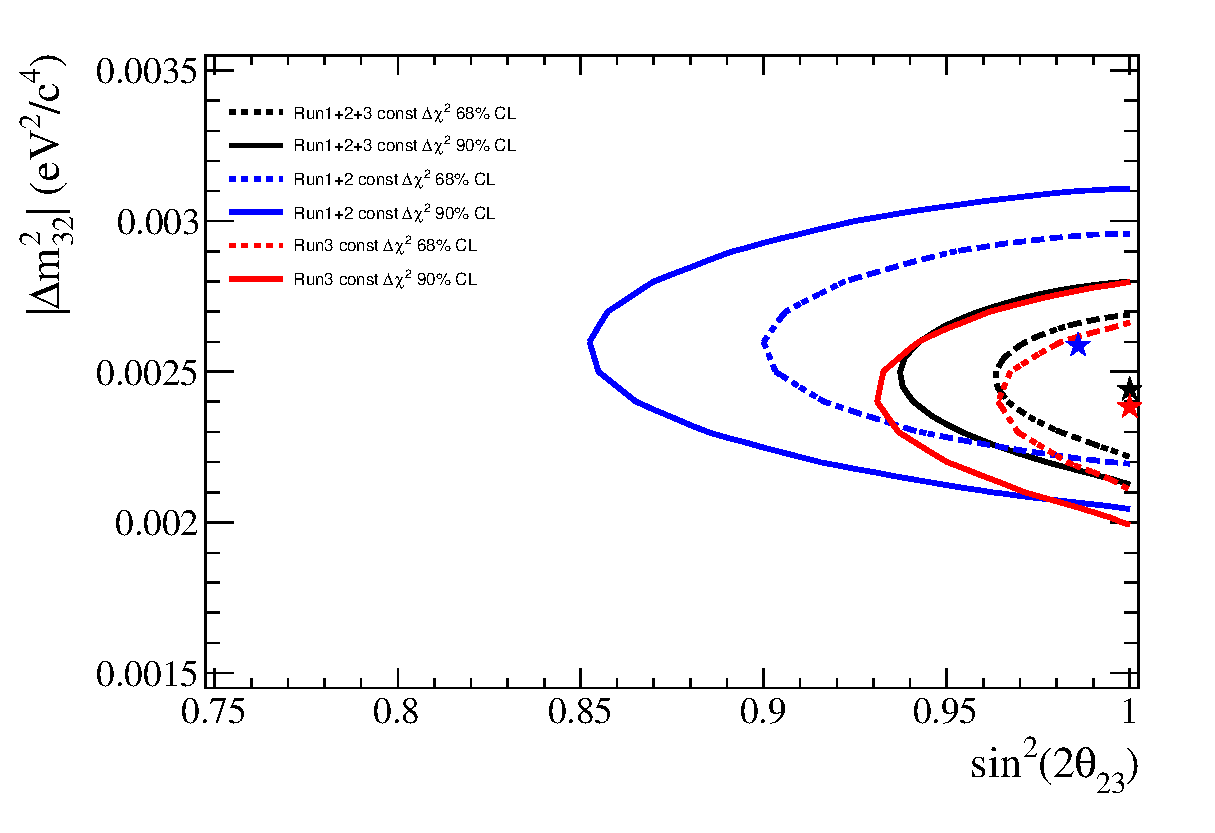
\includegraphics[width=30pc]{./images/fit_data/compare/compare_runs_2N}
\caption {
  Comparison between the 68\% CL and 90\% CL allowed regions obtained from separate
  `2+N' analyses of the Run 1+2+3, Run 1+2 and Run 3 datasets.
  All contours shown were calculated with the constant-$\Delta\chi^2$ method.
}
\label{fig:results_compare_runs_2N}
\end{figure*}

%......................
%
% Run1+2+3 vs Run1+2 vs Run3, 2+8
%
\begin{figure*}[htb]
\center
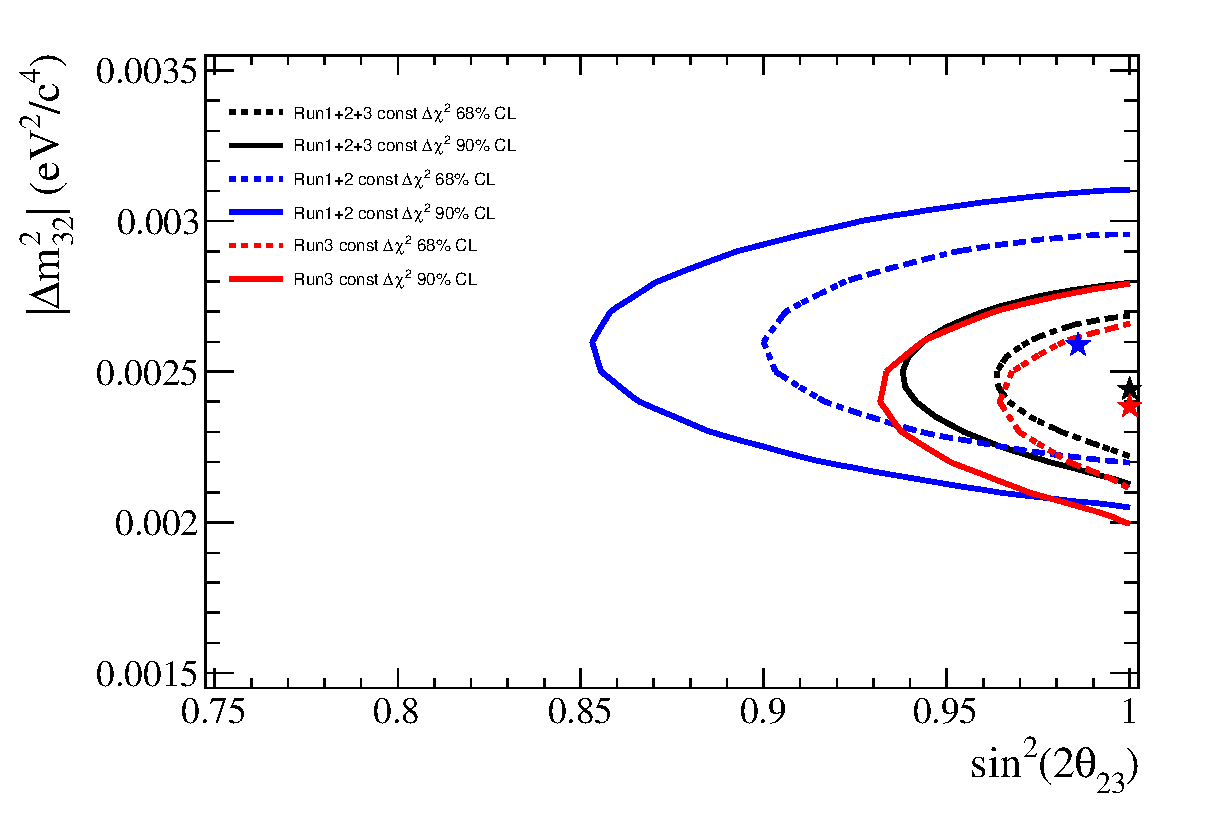
\includegraphics[width=30pc]{./images/fit_data/compare/compare_runs}
\caption {
  Comparison between the 68\% CL and 90\% CL allowed regions obtained from separate
  `2+8' analyses of the Run 1+2+3, Run 1+2 and Run 3 datasets.
  All contours shown were calculated with the constant-$\Delta\chi^2$ method.
}
\label{fig:results_compare_runs}
\end{figure*}


\clearpage

%--------------------------------------------------------------------------------------
% Our views
%--------------------------------------------------------------------------------------

\subsection {The VaLOR group perspective on the choice of primary result}
\label{sec:primary_result_selection}

Four separate $\nu_{\mu}$-disappearance results have been produced by this analysis
for the Run 1+2+3 dataset; this is because we have used two fitting methods 
(`2+N' and `2+8') and two methods for constructing confidence regions (constant-$\Delta\chi^{2}$ 
and Feldman-Cousins).

This analysis used contours produced with the constant-$\Delta\chi^{2}$ method quite extensively, 
especially during its development and for the sensitivity studies. We considered that producing Feldman-Cousins 
contours at an early stage would not be the best use of our time or of the CPU resources available to us. 
In that respect, the constant-$\Delta\chi^{2}$ contours were invaluable as a tool for 
developing the analysis.
The constant-$\Delta\chi^{2}$ contours meet some, but not all of the requirements set by the
muon-neutrino contour committee: they should have correct coverage,
they should be standard in the field and easy to explain,
they should avoid paradoxical results and should be computationally feasible \cite{T2KNuMuContourCom}. However
our group has been a strong advocate of the use of the Feldman-Cousins method from the
time of the Run 1 analysis. Since the best-fit value of $\sin^{2}{2\theta_{23}}$ is at the physical boundary, 
the constant-$\Delta\chi^{2}$ contours do not have correct coverage with present statistics
and we do not consider them as contenders for our primary result.

This leaves only two options to consider: 
The `2+N' and the `2+8' Feldman-Cousins contours.
As shown in this paper, 
no real difference exists between the `2+N' and the `2+8' results:
\begin{itemize}
\item The best-fit points are identical for the combined Run 1+2+3 dataset 
      (and nearly identical for the separate fits to the Run 1+2 and Run 3 datasets),
      as shown in Tab.\ \ref{tab:data_fits:best_fit_values}.
\item The p-values for the fits to the combined Run 1+2+3 dataset are identical,
      as shown in Tab.\ \ref{tab:data_fits:best_fit_values}.
\item Although all 48 systematic parameters are allowed to float in the `2+N' fit,
      only 6 parameters have best-fit values which are more that 
      $\pm$0.1$\sigma$ away from their corresponding nominal values,
      as shown in Fig.\ \ref{fig:results_data123_pulls_2N}.
      Thus the vast majority of the systematic parameters included in the `2+N' fit have,
      in fact, a negligible effect on the fit.
\item The best-fit spectra are indistinguishable when superimposed on the same plot,
      as shown in Fig.\ \ref{fig:results_data123_spectrum_comparison}.
      The best-fit spectra (binned using the same scheme used in the fit) 
      never differ by more than 1.5\% in the area below 3 GeV,
      and they are nearly identical in the area of the first oscillation maximum.
\item The 68\% and 90\% CL regions for the two fits are identical,
      as shown in Figs.\ \ref{fig:results_compare_contours_28_2N} 
      and \ref{fig:results_compare_fc_contours_28_2N}.
      Indeed, the `2+N' and `2+8' marginalized $\Delta\chi^2$ distributions for 
      are identical for both $\sin^{2}{2\theta_{23}}$ and $|\Delta m_{32}^{2}|$, 
      even in areas of the oscillation parameter space outside the 
      99\% CL region (this is defined by $\Delta\chi^2 <$ 6.63 for a single parameter).
      This is shown in Figs.\ 
      \ref{fig:results_comp_marg_dchisq_dmsq_run123} and 
      \ref{fig:results_comp_marg_dchisq_sinsq_run123}.
\end{itemize}

Given the marked similarity of the results of the '2+8' and '2+N' fits, it is difficult to make 
a choice between them. However the VaLOR group prefers the simpler '2+8' fit since it has fewer 
floating parameters. The choice of the 8 floating parameters in this fit was made with an 
extremely careful study which is presented in Sec.\ \ref{sec:fit_syst_analysis}. 

Ockham's razor states that "Pluralitas non est ponenda sine neccesitate" or "Plurality should not be posited 
without necessity" \cite{ockham}. The plurality of the additional floating parameters in the '2+N' fit is unnecessary 
since it does not change the values of the oscillation parameters we seek to measure. Furthermore, the simpler fit 
is easier to explain to a wider audience. For these reasons, we feel strongly that the `2+8' result 
should be the one presented as the official result outside the T2K collaboration.



% Summary and acknowledgements
\clearpage

% --------------------------------------------------------------------------------------------

\section {Summary}
\label{sec:summary}

In this technical note,
we have presented the results of a 3-flavour $\nu_{\mu}$-disappearance analysis,
performed by the Valencia-Lancaster-Oxford-Rutherford (VaLOR) group,
on the combined Run1+2+3 (3.010$\times$10$^{20}$ POT) dataset.
This analysis is an update of the work presented in
Refs. \cite{OurRun1DisappAnalysis}, \cite{OurRun12DisappAnalysis} and \cite{OurRun12DisappAnalysis3Flavour}
with improved methods and an enlarged dataset.

This analysis predicts 204.75 $\pm$ 16.75 (syst)
1 $\mu$-like ring events in SuperK in the absence of any oscillation,
but only 58 were observed. The observed deficit has a strong energy dependence;
the ratio of observed to expected, under the no oscillation hypothesis, is
$\sim$30\% $<$ 0.5 GeV, 
$\sim$10\% between 0.5 and 1 GeV and 
$\sim$75\% $>$ 1 GeV.

A $\nu_{\mu}$-disappearance analysis was performed 
in a framework of 3-flavour oscillations including matter effects in constant-density matter.
A total of 48 efficiency, energy scale, neutrino flux, neutrino cross-section,
initial-state nuclear environment and final-state rescattering systematics was taken into account.
The effect of these systematic uncertainties on the expected number of 1 $\mu$-like ring events,
on their reconstructed energy spectrum and on our oscillation measurement were presented in great detail.

Two versions of the oscillation fit were performed: the `2+N' fit allowed all 48 systematics considered 
in this analysis to float, whereas the `2+8' fit allowed only the 8 most dominant systematics to float. 
The dominant systematics are those identified as having an effect on the measured oscillation parameters 
that is greater than 25\% of the expected statistical error, for at least one set of true oscillation 
parameters in the area of interest. The `2+N' 3-flavour $\nu_{\mu}$-disappearance fit to
the observed reconstructed energy spectrum of 1 $\mu$-like ring events of the combined Run1+2+3 dataset,
for $\sin^2\theta_{23}$ yield
$|\Delta m^{2}_{32}|$ = 2.441$\times$10$^{-3}$ $eV^{2}/c^{4}$  and
$\sin^{2}\theta_{23}$ = 0.514
as the best-fit values (p-value = 0.80).
For the '2+N' fit assuming the first octant ($\sin^22\theta_{23} \geq 0.5$),
with $sin^{2}2\theta_{23}$ constrained to the physical region,
the best-fit values are almost identical at
$|\Delta m^{2}_{32}|$ = 2.443$\times$10$^{-3}$ $eV^{2}/c^{4}$  and
$\sin^{2}2\theta_{23}$ = 1.000
(p-value = 0.83).
For the '2+N' fit assuming the second octant ($\sin^22\theta_{23} \geq 0.5$),
the best-fit values are almost identical at
$|\Delta m^{2}_{32}|$ = 2.441$\times$10$^{-3}$ $eV^{2}/c^{4}$  and
$\sin^{2}2\theta_{23}$ = 0.999
(p-value = 0.82).
For the `2+8' fit, the best-fit values are almost identical.
% at 
% $|\Delta m^{2}_{32}|$ = 2.442$\times$10$^{-3}$ $eV^{2}/c^{4}$  and
% $\sin^{2}2\theta_{23}$ = 1.000
% (p-value = 0.82).
All fits used the 2012 PDG values for
$\sin^{2}2\theta_{13}$, $\sin^{2}2\theta_{12}$ and $\Delta m^{2}_{21}$ \cite{PDG2012},
and assumed $\delta_{CP}$=0 and the normal mass hierarchy.

Confidence regions obtained using both the constant-$\Delta\chi^2$ method and the 
method of Feldman and Cousins were presented for both the `2+N' and `2+8' fits.
% Using the marginalized $\Delta\chi^2$ distributions obtained from the fits,
% and the constant-$\Delta\chi^2$ method,
% the 90\% CL allowed region, for both `2+N' and `2+8' fits, assuming the first octant, can be summarized as
% 2.14$\times$10$^{-3}$ $eV^{2}/c^{4}$ $< |\Delta m^{2}_{32}| < $ 2.76$\times$10$^{-3}$ $eV^{2}/c^{4}$ and
% $\sin^{2}2\theta_{23} > $ 0.957.
% The 90\% CL allowed region, for the '2+N' fit, assuming the second octant, can be summarized as
% 2.??$\times$10$^{-3}$ $eV^{2}/c^{4}$ $< |\Delta m^{2}_{32}| < $ 2.??$\times$10$^{-3}$ $eV^{2}/c^{4}$ and
% $\sin^{2}2\theta_{23} > $ 0.???.
Using the results of the '1+N' fits, 
and the constant-$\Delta\chi^2$ method,
the 90\% CL allowed region, for the `2+N' fit for $\sin^2\theta_{23}$, can be summarized as
$2.19$$\times$10$^{-3}$ eV$^{2}$/c$^{4}$ $< |\Delta m^2_{32}| < 2.72$$\times$10$^{-3}$ eV$^{2}$/c$^{4}$ and
$0.397 < \sin^{2}\theta_{23} < 0.630$.
The corresponding limits for the '2+N' fit assuming the first octant, can be summarized as
$2.19$$\times$10$^{-3}$ eV$^{2}$/c$^{4}$ $< |\Delta m^2_{32}| < 2.72$$\times$10$^{-3}$ eV$^{2}$/c$^{4}$ and
$\sin^{2}2\theta_{23}$ $>$ 0.958.
The corresponding limits for the '2+N' fit assuming the second octant, can be summarized as
$2.19$$\times$10$^{-3}$ eV$^{2}$/c$^{4}$ $< |\Delta m^2_{32}| < 2.72$$\times$10$^{-3}$ eV$^{2}$/c$^{4}$ and
$\sin^{2}2\theta_{23}$ $>$ 0.931.

Numerous comparisons were made of the best-fit values and spectra, of the systematic parameter pulls,
and of the $\chi^{2}$ surfaces obtained by the different fit methods and for different running periods.
Detailed comparisons were presented of the confidence regions obtained
by using different construction methods, for the same fit, and
by using different fitting methods, for the same construction method.
The contours from different running periods were compared.
Comparisons of our contours with
recent measurements from MINOS and SuperK and the T2K 3.010$\times$10$^{20}$-POT sensitivity
were also made. Finally, a more critical view of the 4 different results obtained by
this analysis was presented in Sec.\ \ref{sec:primary_result_selection}.



% --------------------------------------------------------------------------------------------

%
%\section* {Acknowledgements}
%\label{sec:acknowledgements}
%


% References
%
% References
%

\begin{thebibliography}{9}

%
% Our previous analyses
%
\bibitem{OurRun1DisappAnalysis}
   C.Andreopoulos, T.Dealtry, J.Dobson, N.Grant, M.Haigh, J.Ilic, G.Pearce and A.Weber,
   T2K 3.23$\times10^{19}$-POT Muon-Neutrino Disappearance Analysis,
   T2K-TN-036(v4),\\
   http://www.t2k.org/docs/technotes/036
\bibitem{OurRun12DisappAnalysis}
   C.Andreopoulos, T.Dealtry, J.Dobson, N.Grant, M.Haigh, J.Ilic, G.Pearce and A.Weber,
   T2K 1.431$\times10^{20}$-POT Muon-Neutrino Disappearance Analysis
   T2K-TN-064(v3),\\
   http://www.t2k.org/docs/technotes/064
\bibitem{OurRun12DisappAnalysis3Flavour}
   C.Andreopoulos, T.Dealtry, L.Escudero and N.Grant,
   T2K 1.431$\times10^{20}$-POT 3-Flavour Muon-Neutrino Disappearance Analysis
   T2K-TN-087(v1),\\
   http://www.t2k.org/docs/technotes/087
\bibitem{OurRun12JointOscillationAnalysis}
   C.Andreopoulos, A.Cervera, T.Dealtry, L.Escudero, N.Grant, M.Sorel and P.Stamoulis,
   T2K 1.431$\times10^{20}$-POT Joint 3-Flavour Oscillation Analysis
   T2K-TN-133(v1),\\
   http://www.t2k.org/docs/technotes/133
 \bibitem{OurRun123JointOscillationAnalysis}
   C.Andreopoulos, A.Cervera, T.Dealtry, L.Escudero, N.Grant, M.Sorel and P.Stamoulis,
   T2K 3.010$\times10^{20}$-POT Joint 3-Flavour Oscillation Analysis
   T2K-TN-154(v2),\\
   http://www.t2k.org/docs/technotes/154
 \bibitem{OurRun1234aDisappAnalysis3Flavour}
   C.Andreopoulos, T.Dealtry, L.Escudero, N.Grant and A.Weber,
   T2K 6.3933$\times10^{20}$-POT 3-Flavour Muon-Neutrino Disappearance Analysis
   T2K-TN-154(v2),\\
   http://www.t2k.org/docs/technotes/155

   % 
% Our previous published analyses
%
\bibitem{T2KRun12Disapp}
   T2K Collaboration (K.Abe et al.), 
   First Muon-Neutirno Disappearance Study with an Off-Axis Beam,
   Phys.Rev.D85:031103, 2012; arXiv:1201.1386
%
% Official 2012 analysis inputs and software packages
%
\bibitem{Neut:ActaP}
  Y.Hayato, A neutrino interaction simulation program library NEUT,
  Acta Phys.Polon.B40:2477-2489,2009.
\bibitem{FluxTuning}
   Beam WG, Flux tuning (11b v3.2), http://www.t2k.org/beam/NuFlux/FluxRelease/11brelease/11btuned-v3.2
\bibitem{SuperkErrors}
   M.Otani and J.Kameda,
   Super-K events and Updated systematic errors for $\nu_\mu$ disappearance analysis with T2K 1.431$\times10^{20}$ POT
   T2K-TN-065(v6),
   http://www.t2k.org/docs/technotes/065
\bibitem{NEUTnuclear}
  P. de Perio et al.,
  NEUT nuclear effects (FSI)
  T2K-TN-033(v2.0),
  http://www.t2k.org/docs/technotes/033
\bibitem{NIWGErr}
  P. de Perio et al.,
  Cross section parameters for the 2012a oscillation analysis
  T2K-TN-108(v1.3),
  http://www.t2k.org/docs/technotes/108
\bibitem{MoreNIWGErr113}
  P. de Perio et al.,
  Implementation of the NIWG cross-section parametrization,
  T2K-TN-113(v1.2) 
\bibitem{BANFF}
  P. de Perio et al.,
  Constraining the Flux and Cross Section Models with Data from the
  ND280 Detector for the 2012a Oscillation Analysis,
  T2K-TN-106(v8.0)
  http://www.t2k.org/docs/technotes/106
\bibitem{SI}
  P. de Perio et al.,
  Pion Hadronic Secondary Interactions in Super-Kamiokande,
  T2K-TN-105(v1.1)
  http://www.t2k.org/docs/technotes/105
\bibitem{OldDisappSuperK}
  Y. Ashie et al., Phys. Rev. Lett. 93, 101801 (2004);
  Y. Ashie et al., Phys. Rev. D71, 112005 (2005); 
  J. Hosaka et al., Phys. Rev. D 74, 032002 (2006).
\bibitem{SKsample}
  T2KSK,
  http://www.t2k.org/t2ksk/code/sk11c\_mc/sampleinfo.
\bibitem{FluxTuningHistograms}
  Beam group,
  http://www.t2k.org/beam/NuFlux/FluxRelease/11arelease/11atuned-v2.3.
\bibitem{1overMAQE2}
  M. Hartz,
  BANFF Fit Update for the 2012 Disappearance Analyses,
  http://www.t2k.org/asg/meeting/20121015/banffinputsdisapp/view.
%
% External papers relevant to official inputs
%
\bibitem{NA61T2K}
  N Abgrall et al. Measurements of Cross Sections and Charged Pion Spectra in Proton-Carbon Interactions
  at 31 GeV/c. Phys.Rev., C84:034604, 2011;
  N. Abgrall et al. Measurement of production properties of positively charged kaons in proton-carbon
  interactions at 31 GeV/c. arXiv:hep-ex/1112.0150, 2011.
%
% PDG-2012 
%
\bibitem{PDG2012}
  J. Beringer et al. (Particle Data Group), Phys. Rev. D86, 010001 (2012)
%
% Talks by VaLOR group members referenced in the text
%
\bibitem{Lorena}
  Lorena Escudero Sanchez for the VaLOR group, 
  http://www.t2k.org/asg/oagroup/meeting/20121219/VaLOR%202012%20joint%20OA%20report/view
\bibitem{Tom1overMaQE2}
  Tom Dealtry for the VaLOR group,
  http://www.t2k.org/asg/meeting/2012/20121015/valornumudisapp/view
%
% Statistics etc
%
\bibitem{StatAnalysisCowan} 
  G. Cowan (1998) Statistical data analysis, 
  Oxford University Press, ISBN 0-19-850155-2.
\bibitem{Minuit}
  F.James, M.Roos, Minuit: A System for Function Minimization and Analysis of the 
  Parameter Errors and Correlations, Comput.Phys.Commun. 10:343 (1975)
%\bibitem{NumRecipCholesky}
%  Numerical Recipes: The art of scientific computing, 
%  Cambridge University Press, 3rd Edition, ISBN 978-0-521-88068-0, pp. 100-102.
%\bibitem{RevPartPhysStat}
%  C. Amsler et al. (Particle Data Group),
%  Review of Particle Physics, Phys.Lett.B667:1,2008 
\bibitem{FeldmanCousins}
  G.J. Feldman and R.D. Cousins,
  A Unified approach to the classical statistical analysis of small signals,
  Phys.Rev.D57:3873-3889,1998; physics/9711021
\bibitem{CousinsHighland}
  R.D. Cousins and V.L.Highland, 
  Nucl.Instr. and Meth. A320:331035, 1992.
\bibitem{NickPvalue}
  N.Grant for the VaLOR group,
  http://www.t2k.org/asg/meeting/2011/20111124/pvalues/view
\bibitem{KarlenPvalue}
  D.Karlen,
  p-values, distributions and low statistics,
  http://www.t2k.org/asg/oagroup/meeting/20120416/lowstat/view
%
% Numu contour committe report
%
\bibitem{T2KNuMuContourCom}
  K. McFarland for the T2K $\nu_{\mu}$-disappearance contour committee 
  (C.Andreopoulos, N.Grant, J.Kameda, D.Karlen, E.Kearns, K.McFarland, M.Otani, M.Zito)
  Report to ASG conveners meeting, 17 May 2011,
  http://www.t2k.org/asg/contour/ASG-Conveners-Report/view
%
% MINOS, SK atm. "23"-sector oscillation analyses
%
\bibitem{MINOS2012}
  R.Nichol,
  Talk at Neutrino 2012
\bibitem{MINOS2013:3nu}
  A. Radovic,
  Talk at DPF 2013
\bibitem{SKAtm2012}
  Y.Itow,
  Talk at Neutrino 2012
%
% Experiment-specific theta13, theta12, and dmsq12 refs
%
\bibitem{Kamland}
  S. Abe et al.,
  Precision measurements of neutrino oscillation parameters with KamLAND
  Phys.Rev.Lett.100:221803,2008
\bibitem{DayaBay}
  F.P. An et al.,
  Observation of electron-antineutrino disappearance at Daya Bay
  Phys.Rev.Lett.108:171803,2012
\bibitem{Reno}
  J.K. Ahn et al.,
  Observation of reactor electron antineutrinos disappearance in the Reno experiment
  Phys.Rev.Lett.108:191802,2012
%
% Global oscillation analyses
%
\bibitem{FogliLisi}
  G.L.Fogli, E.Lisi et~al.,
  Evidence of theta(13)$>$0 from global neutrino data analysis,
  arXiv:1106.6028 [hep-ph]
\bibitem{GonzalezGarcia}
  M.C.Gonzalez-Garcia, M.Maltoni, J.Salvado and T.Schwetz,
  Global fit to three neutrino mixing: critical look at present precision,
  arXiv:1209.3023 [hep-ph]
\bibitem{ockham}
  "Ockham's razor", Encyclopedia Britannica
  http://www.britannica.com/EBchecked/topic/424706/Ockhams-razor
%
% 3-flavour oscillation probability formulas etc
%
\bibitem{kayser2005}
  B. Kayser (2005), Neutrino physics, hep-ph 0506165
\bibitem{giunti}
  C Giunti and C.W. Kim (2007) Fundamentals of neutrino physics and astrophysics, Oxford Uninversity Press
%\bibitem{pdgreview}
%  K. Nakamura and S.T. Petcov (2010) Neutrino mass, mixing and oscillations,
%  http://pdg.lbl.gov/2010/reviews/rpp2010-rev-neutrino-mixing.pdf
\bibitem{kopp}
  J. Kopp (2006), Efficient numerical diagonalisation of Hermitian 3x3 matrices, arXiv:physics/0610206
%
% Other 3-flavour oscillation probability packages
%
\bibitem{sloan}
  T. Sloan, private communication (June-July 2011)
\bibitem{Prob3}
  Prob3++ 3-flavour oscillation probability software,
  http://www.phy.duke.edu/~raw22/public/Prob3++/

\end{thebibliography}




% Appendices
\clearpage
\appendix
\addappheadtotoc
\clearpage

\section{VaLOR 3-flavour oscillation probability calculations}
\label{appendix:valor_3f_osc_prob_code}

In this analysis, 3-flavour neutrino oscillation probabilities in constant density matter are used. Vacuum 3-flavour oscillation 
probabilites are also calculated, but these are used only to estimate the accuracy of the 3-flavour probabilities in matter (see 
section \ref{sec:3flavouraccuracy}). 
The method of calculation of the vacuum probabilities is given in section \ref{sec:vacuumosc}, while the calculation 
of the probabilities in constant density matter is described in section \ref{sec:matterosc}. The code that makes these calculations 
has been integrated into the VaLOR oscillation analysis package. In section \ref{sec:3flavourresults}, 
comparisons are given between 2-flavour and 3-flavour (in matter) oscillation probabilities, and between 3-flavour oscillation probabilities 
in vacuum and matter. Validation of the code is described in section \ref{sec:3flavourvalidation}: the vacuum probabilities were validated 
by comparing their values with those obtained from an alternative formulation in the PDG review. Several validation checks of 
the probabilities in constant density matter are made as they are calculated, and the values of the probabilities were checked 
by comparing them with those given by an independently-written program. Finally, an estimate of the accuracy of the oscillation 
probabilities in matter is given in section \ref{sec:3flavouraccuracy}.
   
\subsection{3-flavour neutrino oscillation probabilities in vacuum}
\label{sec:vacuumosc}

The 3-flavour neutrino oscillation probabilities in vacuum are calculated from equation 11 in \cite{kayser2005}:
\begin{equation}
P(\nu_{\alpha} \rightarrow \nu_{\beta}) = \delta_{\alpha \beta} - 4 \sum_{i>j} Re(U_{\alpha i}^{*} U_{\beta i} U_{\alpha j} U_{\beta j}^{*})
\sin^{2} \left( \frac{\Delta m_{ij}^{2} L}{4E} \right) + 2 \sum_{i>j} Im(U_{\alpha i}^{*} U_{\beta i} U_{\alpha j} U_{\beta j}^{*})
\sin \left(\frac{\Delta m_{ij}^{2} L}{2E} \right)
\label{3flavouroscprobvacuum}
\end{equation}
In equation \ref{3flavouroscprobvacuum}, $\Delta m_{ij}^{2}$ = $m_{j}^{2}$ - $m_{i}^{2}$, L is the distance from the neutrino target 
in Tokai to Super-K (295 km), E is the neutrino energy, and U is the PMNS matrix in vacuum:

\begin{equation}
U = \left(
\begin{array}{ccc}
c_{12}c_{13} & c_{13}s_{12} & s_{13}e^{-i\delta} \\
-c_{23}s_{12} - s_{13}s_{23}c_{12}e^{i\delta} & c_{12}c_{23} - s_{12}s_{13}s_{23}e^{i\delta} & c_{13}s_{23} \\
s_{12}s_{23} - s_{13}c_{12}c_{23}e^{i\delta} & -s_{23}c_{12} - s_{12}c_{23}s_{13}e^{i\delta} & c_{13}c_{23}
\end{array} \right)
\label{PMNSmatrix}
\end{equation}
with $s_{12} = \sin(\theta_{12})$, $c_{12} = \cos(\theta_{12})$, etc. $P(\bar{\nu}_{\alpha} \rightarrow \bar{\nu}_{\beta})$ 
is calculated by changing the sign of the third term in equation \ref{3flavouroscprobvacuum} (this assumes that CPT is 
conserved).

\subsection{3-flavour neutrino oscillation probabilities in constant density matter}
\label{sec:matterosc}
All three neutrino flavours undergo neutral-current interactions with protons, neutrons and electrons in matter. These 
neutral-current interactions have identical amplitudes for all three flavours, and they produce no observable effects on
the probabilities of oscillation between one flavour and another. However the oscillation probabilities are changed by 
coherent forward scattering of electron neutrinos in charged-current interactions with electrons in matter \cite{kayser2005}.

Using natural units with $\hbar$ = c = 1, the time evolution of neutrino flavour states in vacuum is described by the 
Schr\"odinger equation:

\begin{equation}
i \frac{\partial \mathbf{\psi}}{\partial t} = H_{F} \mathbf{\psi} 
\end{equation}
where
\begin{equation}
  \mathbf{\psi} =\left(
\begin{array}{c}
\psi_{e} \\
\psi_{\mu} \\
\psi_{\tau}
\end{array} \right)
\end{equation}
and $H_{F}$ is the effective Hamiltonian in the flavour-state basis
\begin{equation}
H_{F} = \frac{1}{2E} U M U^{\dagger}
\end{equation}
with M defined by
\begin{equation}
M = \left(
\begin{array}{ccc}
0 & 0 & 0 \\
0 & \Delta m_{21}^{2} & 0 \\
0 & 0 & \Delta m_{31}^{2}
\end{array} \right)
\end{equation}
The calculation of oscillation probabilities requires neutrino flight time to be converted to distance travelled, 
and this conversion assumes that neutrinos are highly relativistic. In 
this calculation, $U M U^{\dagger}$ is used for neutrinos, but its complex conjugate is used for antineutrinos. For neutrinos, 
the effects of the charged-current interactions between electron neutrinos and electrons are taken into account by adding the 
potential $2E \sqrt{2} G_{F} N_{e}$ to the real part of the first diagonal element of $U M U^{\dagger}$, where E is the 
neutrino energy, $G_{F}$ is the Fermi coupling constant, and $N_{e}$ is the number density of electrons in matter. For 
antineutrinos, this potential is subtracted from the real part of the first diagonal element of the complex conjugate of 
$U M U^{\dagger}$ (for further details see section 9.2 in \cite{giunti}). 

After the addition or subtraction of this potential, $U M U^{\dagger}$ (or its complex conjugate) is diagonalised. The eigenvalues 
of a Hermitian matrix are always real; they are calculated by solving the (cubic) characteristic equation using the method 
of del Ferro, Tartaglia and Cardano as described in \cite{kopp}. The differences between the eigenvalues are the effective 
mass-squared differences in matter. The eigenvectors are calculated using an algebraic method: one of the components is set 
to be 1.0 (real), and the other two components are calculated using two of the three simultaneous equations in 
$U M U^{\dagger} - \lambda I = 0$, where the $\lambda$ are the eigenvalues. After being normalised, the three eigenvectors 
become the columns of the effective mixing matrix in matter. 

The initial flavour state of the neutrino is represented by a 1$\times$3 column vector whose entries are complex; if, for 
example, the initial flavour state is a muon neutrino, this column vector is 

\begin{displaymath}
\left(
\begin{array}{c}
0 \\
1 \\
0 
\end{array} \right)
\end{displaymath}
The vector representing the initial flavour state is then multiplied by the Hermitian conjugate of the matter mixing matrix 
to convert it to another 1$\times$3 complex column vector representing the initial mass states. These mass states are propagated 
to Super-K by multiplying the jth initial mass state by $\exp \left(\frac{-i \Delta m_{j1}^{2}L}{2E} \right)$, where the 
$\Delta m_{j1}^{2}$ are the mass-squared differences in matter, i.e.\ the differences between the eigenvalues of $U M U^{\dagger}$. 
This gives a new 1$\times$3 complex column vector representing the final mass states, and these are converted to the final flavour 
states by multiplying by the matter mixing matrix. The entries of the resulting 1$\times$3 complex column vector represent the 
amplitudes of each flavour at Super-K, and the corresponding oscillation probabilities are calculated as the moduli squared of these 
amplitudes.  

\subsection{Inputs to the 3-flavour neutrino oscillation probability calculations}

When calculating the 3-flavour oscillation probabilities, the mixing angles can be input either in the form $\sin^{2}(2 \theta_{ij})$ 
or as $\sin^{2}(\theta_{ij})$. $\sin(\theta_{ij})$ and $\cos(\theta_{ij})$ are calculated from the input values, and these are used in 
turn to calculate the elements of $U$. The ``solar'' mass-squared difference is input as $\Delta m_{21}^{2}$, and this is $>$ 0 for 
both mass hierarchies. The ``atmospheric'' 
mass-squared difference is input either as $|\Delta m_{32}^{2}|$ or using a definition introduced by G.\ Fogli, E.\ Lisi et al.\ in 
\cite{LisiGlobalAnalysis}:
\begin{equation}
\Delta m^{2}_{FL} = m_{3}^{2} - \frac{m_{2}^{2} + m_{1}^{2}}{2}
\end{equation}
The quantity denoted $\Delta m^{2}_{FL}$ is useful since its absolute value is the same for both mass hierarchies, and only its sign 
changes. If the atmospheric mass-squared difference is input as $\Delta m^{2}_{32}$, the mass hierarchy is set using the sign of 
$\Delta m_{32}^{2}$; this is positive for the normal mass hierarchy (NH) and negative for the inverted mass hierarchy (IH). In this case, 
$\Delta m_{31}^{2}$ is not input but is calculated as $\Delta m_{31}^{2}$ = $\Delta m_{21}^{2}$ + $\Delta m_{32}^{2}$ for both hierarchies.
If the atmospheric mass-squared difference is input as $\Delta m^{2}_{FL}$, the mass hierarchy is set using the sign of $\Delta m^{2}_{FL}$. 
Then $\Delta m_{32}^{2}$ and $\Delta m_{31}^{2}$ are calculated from the input values of $\Delta m^{2}_{FL}$ and $\Delta m_{21}^{2}$.

\subsection{Results of the 3-flavour neutrino oscillation probability calculations}
\label{sec:3flavourresults}

A comparison of 2-flavour and 3-flavour (in matter) $\nu_{\mu}$-survival probabilities is given in figure \ref{pnumunumucomp}. 
In this figure, the nominal probabilities are calculated with $\sin^{2}(2 \theta_{12})$ = 0.87, $\sin^{2}(2 \theta_{13})$ = 0.1,
$\sin^{2}(2 \theta_{23})$ = 1.0, $\Delta m_{21}^{2}$ = 7.6 $\times 10^{-5}$  eV$^{2}$/c$^{4}$, $|\Delta m_{32}^{2}|$ = 2.32 $\times$ 10$^{-3}$ eV$^{2}$/c$^{4}$,
$\delta_{CP}$ = 0 and Earth crust density = 2.6 g/cm$^{3}$. The bands represent the maximum and minimum 3-flavour probabilities from 4000 random
variations of the non-23 oscillation parameters within their uncertainties at each energy with the same values of $\sin^{2}(2 \theta_{23})$ and
$|\Delta m_{32}^{2}|$ being used. The uncertainties in $\sin^{2}(2 \theta_{12})$ and $\Delta m_{21}^{2}$ are taken from KamLAND combined
with solar experiments \cite{Kamland}, while those in $\sin^{2}(2 \theta_{13})$ are computed as a weighted average of measurements from Daya Bay
\cite{DayaBay} and Reno \cite{Reno}.

The effect of $\sin^{2}(2 \theta_{13})$ on the 3-flavour $\nu_{\mu}$-survival probability in matter 
is shown in figure \ref{pnumunumus13}: there is a small increase in P($\nu_{\mu} \rightarrow \nu_{\mu}$) at all energies as 
$\sin^{2}(2 \theta_{13})$ increases. Also shown in figure \ref{pnumunumudelta} is the effect of $\delta_{CP}$ on the 3-flavour $\nu_{\mu}$-survival 
probability in matter: as $\delta_{CP}$ increases from 0 to $\pi$, P($\nu_{\mu}\rightarrow\nu_{\mu}$) increases above the oscillation 
maximum and decreases below it for the NH, with these changes being reversed for the IH. 
%A similar comparison for P($\nu_{\mu} \rightarrow \nu_{e}$) in matter is given in figure \ref{pnumunuecomp}, and the effect of $\delta_{CP}$ on
%P($\nu_{\mu} \rightarrow \nu_{e}$) in matter is given in figure \ref{pnumunuedelta}. 
The effects of uncertainties in $\sin^{2}(2 \theta_{12})$ and $\Delta m_{21}^{2}$ on the 3-flavour P($\nu_{\mu}\rightarrow\nu_{\mu}$) in matter 
are shown for the NH in table \ref{numuSurvProbEffectError12}. At 0.6 GeV, uncertainties in $\sin^{2}(2 \theta_{12})$ change 
P($\nu_{\mu}\rightarrow\nu_{\mu}$) by $\approx$ 0.00025 and uncertainties in $\Delta m_{21}^{2}$ change it by $\approx$ 0.0001. 

For the NH, the 3-flavour P($\nu_{\mu}\rightarrow\nu_{\mu}$) is increased below the oscillation
maximum and decreased above it compared with the 2-flavour probability, while for the IH these changes are reversed. The oscillation maximum is at
lower energy for the IH than for the NH, and this can be understood more easily by considering the vacuum probabilities. In equation 
\ref{3flavouroscprobvacuum}, the imaginary terms are zero if $\alpha$ = $\beta$, and only the 3 real terms contribute to the vacuum P($\nu_{\mu} \rightarrow \nu_{\mu}$). 
If the atmospheric mass-squared difference is input as $\Delta m^{2}_{32}$, the terms $|U_{\mu 1}|^{2}$, $|U_{\mu 2}|^{2}$, $|U_{\mu 3}|^{2}$, 
$sin^{2} \left( \frac{\Delta m_{21}^{2} L}{4E} \right)$ and sin$^{2} \left( \frac{\Delta m_{32}^{2} L}{4E} \right)$ are identical for the two hierarchies, 
and the only term that changes between them is sin$^{2} \left( \frac{\Delta m_{31}^{2} L}{4E} \right)$. Since $\Delta m_{31}^{2}$ is lower for the 
IH than for the NH, sin$^{2} \left( \frac{\Delta m_{31}^{2} L}{4E} \right)$ has its maximum at a lower energy for the IH than for the NH. The vacuum 
P($\nu_{\mu}\rightarrow\nu_{\mu}$) depends on 1 - 4 $|U_{\mu 1}|^{2}$$|U_{\mu 3}|^{2}$ sin$^{2} \left( \frac{\Delta m_{31}^{2} L}{4E} \right)$, which means that its minimum is 
at a lower energy for the IH than for the NH.     

Referring to the bands in figure \ref{pnumunumucomp}, the highest $\nu_{\mu}$-survival probabilities for the NH are for low values of $\sin^{2}(2 \theta_{12})$, 
high values of $\sin^{2}(2 \theta_{13})$ and $\delta_{CP}$ near $\pi$ above the oscillation maximum, while below the maximum they are for high values of 
$\sin^{2}(2 \theta_{12})$ and $\sin^{2}(2 \theta_{13})$ and $\delta_{CP}$ near 0. For the IH, the highest probabilities 
are for high values of $\sin^{2}(2 \theta_{12})$ and $\sin^{2}(2 \theta_{13})$ and $\delta_{CP}$ near 0 above the oscillation maximum, but 
for low values of $\sin^{2}(2 \theta_{12})$, high values of $\sin^{2}(2 \theta_{13})$ and $\delta_{CP}$ near $\pi$ below it.

Comparisons of $\nu_{\mu}$ oscillation probabilities 
in vacuum and matter are given for the NH in table \ref{numuOscMatterEffectsNH} and for the IH in 
table \ref{numuOscMatterEffectsIH}. At 0.6 GeV, P($\nu_{\mu}\rightarrow\nu_{e}$) is increased by $\approx$ 0.004 and 
P($\nu_{\mu}\rightarrow\nu_{\tau}$) is decreased by $\approx$ 0.004 in matter compared with vacuum for the NH, while for the 
IH the changes are once more reversed. The $\nu_{\mu}$-survival probability is relatively unaffected by the passage of 
$\nu_{\mu}$ through matter, and is changed by only $\approx$ 0.0001 compared with the vacuum probability at 0.6 GeV.

\begin{figure}
\begin{center}
\resizebox{14cm}{!}{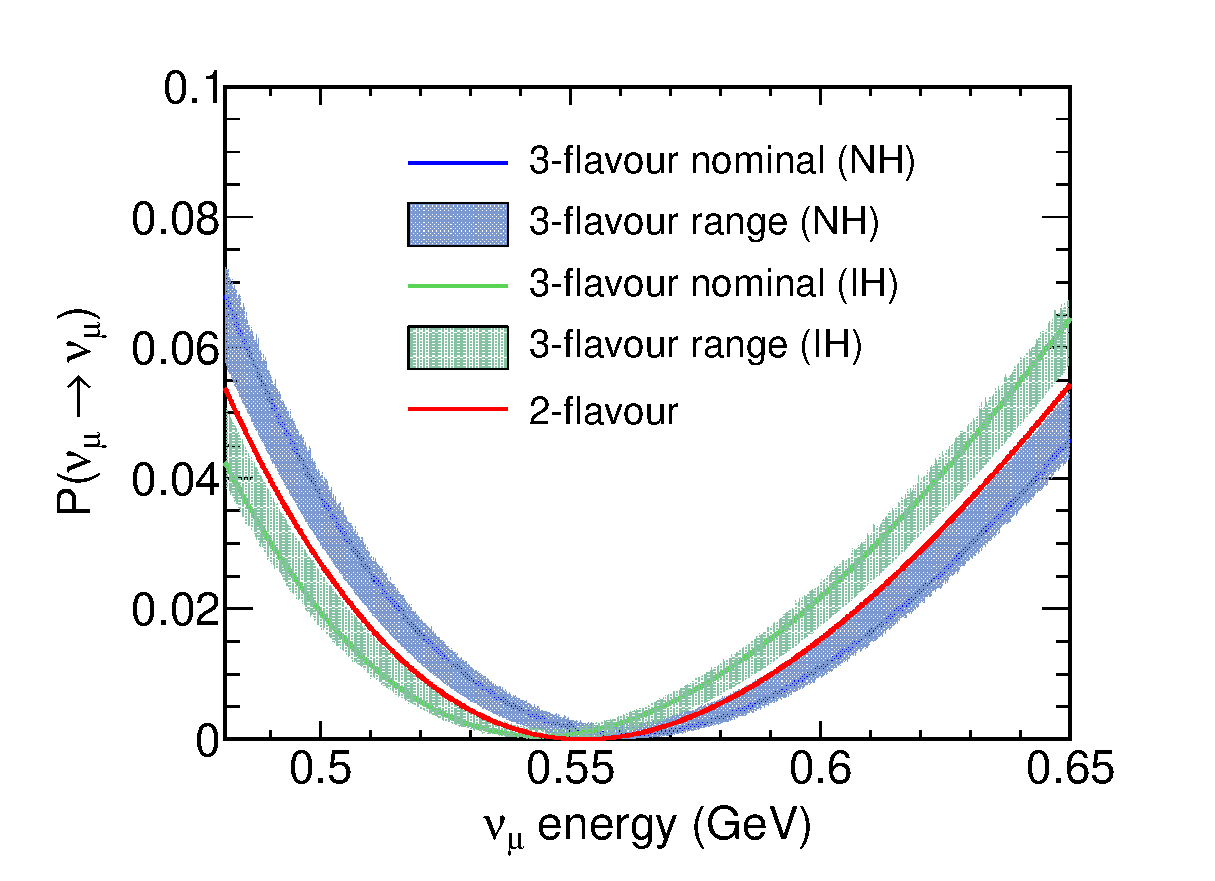
\includegraphics{./images/osc_prob/Prob3NumuSurv.eps}}
\caption[Comparison of P($\nu_{\mu} \rightarrow \nu_{\mu}$) for 2-flavour and 3-flavour (in matter) oscillations]
{Comparison of P($\nu_{\mu} \rightarrow \nu_{\mu}$) for 2-flavour and 3-flavour (in matter) oscillations, NH = normal mass hierarchy,
IH = inverted mass hierarchy. The nominal probabilities are calculated with $\sin^{2}(2 \theta_{12})$ = 0.87, $\sin^{2}(2 \theta_{13})$ = 0.1, 
$\sin^{2}(2 \theta_{23})$ = 1.0, $\Delta m_{21}^{2}$ = 7.6 $\times 10^{-5}$  eV$^{2}$/c$^{4}$, $|\Delta m_{32}^{2}|$ = 2.32 $\times$ 10$^{-3}$ eV$^{2}$/c$^{4}$, 
$\delta_{CP}$ = 0 and Earth crust density = 2.6 g/cm$^{3}$. The bands represent the maximum and minimum 3-flavour probabilities from 4000 random 
variations of the non-23 oscillation parameters within their uncertainties at each energy with the same values of $\sin^{2}(2 \theta_{23})$ and 
$|\Delta m_{32}^{2}|$ being used.}
\label{pnumunumucomp}
\end{center}
\end{figure}

\begin{figure}[ht]
\begin{minipage}[t]{0.48\linewidth}
\centering
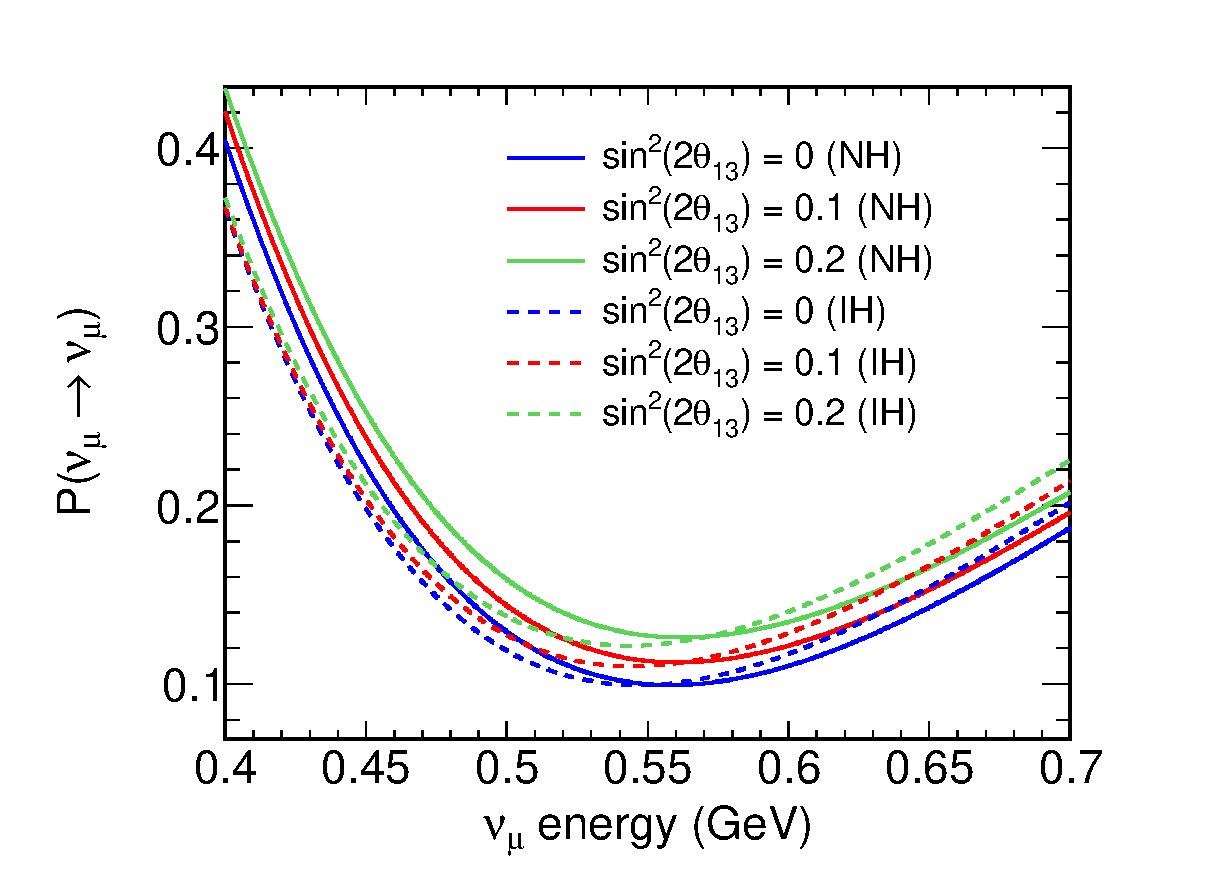
\includegraphics[width=19pc,height=18pc]{./images/osc_prob/Prob3NumuSurvS13.eps}
\caption{
  Effect of $\sin^{2}(2 \theta_{13})$ on P($\nu_{\mu} \rightarrow \nu_{\mu}$) for 3-flavour oscillations in matter; 
  NH = normal mass hierarchy, IH = inverted mass hierarchy, $\sin^{2}(2 \theta_{12})$ = 0.87, $\sin^{2}(2 \theta_{23})$ = 1.0,
  $\Delta m_{21}^{2}$ = 7.6 $\times 10^{-5}$ eV$^{2}$/c$^{4}$, $|\Delta m_{32}^{2}|$ = 2.32 $\times$ 10$^{-3}$ eV$^{2}$/c$^{4}$, $\delta_{CP}$ = 0
  and Earth crust density = 2.6 g/cm$^{3}$.
}
\label{pnumunumus13}
\end{minipage}
\hspace{0.04\linewidth}
\begin{minipage}[t]{0.48\linewidth}
\centering
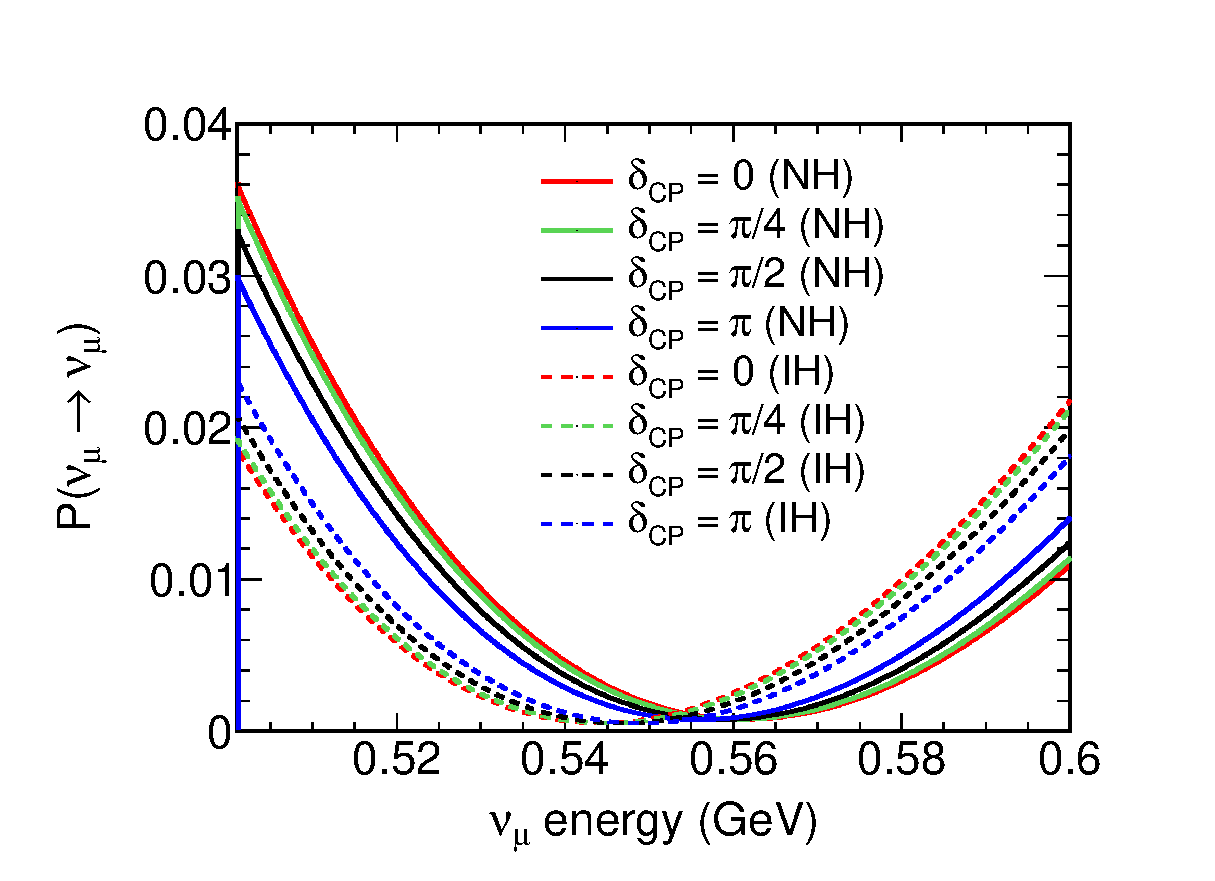
\includegraphics[width=19pc,height=19pc]{./images/osc_prob/Prob3NumuSurvDeltaCP0506.eps}
\caption{
  Effect of $\delta_{CP}$ on P($\nu_{\mu} \rightarrow \nu_{\mu}$) for 3-flavour oscillations in matter; NH = normal mass hierarchy,
  IH = inverted mass hierarchy, $\sin^{2}(2 \theta_{12})$ = 0.87, $\sin^{2}(2 \theta_{13})$ = 0.1, $\sin^{2}(2 \theta_{23})$ = 1.0,
  $\Delta m_{21}^{2}$ = 7.6 $\times 10^{-5}$  eV$^{2}$/c$^{4}$, $|\Delta m_{32}^{2}|$ = 2.32 $\times$ 10$^{-3}$ eV$^{2}$/c$^{4}$ 
  and Earth crust density = 2.6 g/cm$^{3}$.
}
\label{pnumunumudelta}
\end{minipage}
\end{figure}

\begin{table}
\centering
\begin{tabular}{| c | c | c | c | c | c |}
\hline
Energy & P($\nu_{\mu} \rightarrow \nu_{\mu}$) & P($\nu_{\mu} \rightarrow \nu_{\mu}$) &
       P($\nu_{\mu} \rightarrow \nu_{\mu}$) & P($\nu_{\mu} \rightarrow \nu_{\mu}$) & P($\nu_{\mu} \rightarrow \nu_{\mu}$) \\
(GeV) & for $\sin^{2}(2 \theta_{12})$ & for $\sin^{2}(2 \theta_{12})$ & for $\sin^{2}(2 \theta_{12})$
             & for $\sin^{2}(2 \theta_{12})$ & for $\sin^{2}(2 \theta_{12})$ \\
  & = 0.870, & = 0.906, & = 0.833, & = 0.870, & = 0.870, \\
  & $\Delta m_{21}^{2}$ = &  $\Delta m_{21}^{2}$ = & $\Delta m_{21}^{2}$ = & $\Delta m_{21}^{2}$ = & $\Delta m_{21}^{2}$ = \\
  & 7.6 $\times 10^{-5}$  eV$^{2}$/c$^{4}$ & 7.6 $\times 10^{-5}$  eV$^{2}$/c$^{4}$ & 7.6 $\times 10^{-5}$  eV$^{2}$/c$^{4}$ 
   & 7.8 $\times 10^{-5}$ eV$^{2}$/c$^{4}$ & 7.4 $\times 10^{-5}$  eV$^{2}$/c$^{4}$ \\
\hline
0.3 &  0.95703 &  0.95809 &  0.95608 &  0.95733 &  0.95674 \\
\hline
0.4 &  0.35053 &  0.35247 &  0.34877 &  0.35135 &  0.34971 \\
\hline
0.5 &  0.037395 &  0.038009 &  0.036842 &  0.037663 &  0.037129 \\
\hline
0.6 &  0.010963 &  0.010692 &  0.011212 &  0.010841 &  0.011086 \\
\hline
0.7 &  0.094387 &  0.093711 &  0.095004 &  0.094083 &  0.094691 \\
\hline
0.8 &  0.20453 &  0.20371 &  0.20528 &  0.20416 &  0.20490 \\
\hline
0.9 &  0.31099 &  0.31015 &  0.31175 &  0.31061 &  0.31137 \\
\hline
1.0 &  0.40463 &  0.40383 &  0.40535 &  0.40427 &  0.40499 \\
\hline
1.1 &  0.48414 &  0.48340 &  0.48481 &  0.48380 &  0.48447 \\
\hline
1.2 &  0.55080 &  0.55013 &  0.55141 &  0.55050 &  0.55111 \\
\hline
1.3 &  0.60656 &  0.60594 &  0.60711 &  0.60628 &  0.60683 \\
\hline
1.4 &  0.65329 &  0.65274 &  0.65380 &  0.65304 &  0.65354 \\
\hline
1.5 &  0.69265 &  0.69215 &  0.69311 &  0.69243 &  0.69288 \\
\hline
1.6 &  0.72599 &  0.72554 &  0.72640 &  0.72579 &  0.72620 \\
\hline
1.7 &  0.75440 &  0.75399 &  0.75478 &  0.75421 &  0.75459 \\
\hline
1.8 &  0.77876 &  0.77839 &  0.77910 &  0.77859 &  0.77893 \\
\hline
1.9 &  0.79978 &  0.79943 &  0.80009 &  0.79962 &  0.79993 \\
\hline
2.0 &  0.81801 &  0.81770 &  0.81830 &  0.81787 &  0.81815 \\
\hline
\end{tabular}
\caption{
  Effects of uncertainties in $\sin^{2}(2 \theta_{12})$ and $\Delta m_{21}^{2}$ 
  on the 3-flavour P($\nu_{\mu} \rightarrow \nu_{\mu}$) in matter; this is for the normal mass hierarchy, $\sin^{2}(2 \theta_{23})$ = 1.0, 
  $|\Delta m_{32}^{2}|$ = 2.32 $\times$ 10$^{-3}$ eV$^{2}$/c$^{4}$, $\sin^{2}(2 \theta_{13})$ = 0.1 and $\delta_{CP}$ = 0.
}
\label{numuSurvProbEffectError12}
\end{table}

\clearpage

\begin{table}
\centering
\begin{tabular}{| c | c | c | c | c | c | c |}
\hline
Energy (GeV) & \multicolumn{2}{|c|}{P($\nu_{\mu} \rightarrow \nu_{e}$)} & \multicolumn{2}{|c|}{P($\nu_{\mu} \rightarrow \nu_{\mu}$)} & \multicolumn{2}{|c|}{P($\nu_{\mu} \rightarrow \nu_{\tau}$)}\\
\hline
 & Vacuum & Matter & Vacuum & Matter & Vacuum & Matter \\
\hline
0.3 &  0.00054403 &  0.00016981 &  0.95496 &  0.95703 &  0.044501 &  0.042796\\
\hline
0.4 &  0.024253 &  0.029051 &  0.34954 &  0.35053 &  0.62621 &  0.62042\\
\hline
0.5 &  0.046291 &  0.051402 &  0.037071 &  0.037395 &  0.91664 &  0.91120\\
\hline
0.6 &  0.051975 &  0.056108 &  0.010883 &  0.010963 &  0.93714 &  0.93293\\
\hline
0.7 &  0.049739 &  0.052871 &  0.094385 &  0.094387 &  0.85588 &  0.85274\\
\hline
0.8 &  0.044830 &  0.047181 &  0.20455 &  0.20453 &  0.75062 &  0.74829\\
\hline
0.9 &  0.039478 &  0.041256 &  0.31101 &  0.31099 &  0.64951 &  0.64776\\
\hline
1.0 &  0.034502 &  0.035865 &  0.40464 &  0.40463 &  0.56085 &  0.55951\\
\hline
1.1 &  0.030139 &  0.031200 &  0.48415 &  0.48414 &  0.48571 &  0.48466\\
\hline
1.2 &  0.026403 &  0.027241 &  0.55081 &  0.55080 &  0.42279 &  0.42196\\
\hline
1.3 &  0.023233 &  0.023905 &  0.60656 &  0.60656 &  0.37021 &  0.36954\\
\hline
1.4 &  0.020548 &  0.021093 &  0.65329 &  0.65329 &  0.32616 &  0.32562\\
\hline
1.5 &  0.018268 &  0.018715 &  0.69266 &  0.69266 &  0.28908 &  0.28863\\
\hline
1.6 &  0.016325 &  0.016696 &  0.72599 &  0.72599 &  0.25769 &  0.25731\\
\hline
1.7 &  0.014661 &  0.014971 &  0.75440 &  0.75440 &  0.23094 &  0.23063\\
\hline
1.8 &  0.013228 &  0.013491 &  0.77876 &  0.77876 &  0.20801 &  0.20775\\
\hline
1.9 &  0.011988 &  0.012211 &  0.79977 &  0.79978 &  0.18824 &  0.18801\\
\hline
2.0 &  0.010908 &  0.011100 &  0.81801 &  0.81801 &  0.17108 &  0.17089\\
\hline
\end{tabular}
\caption{
 Comparison of $\nu_{\mu}$ oscillation probabilities in vacuum and matter for the normal mass hierarchy, Earth crust
 density = 2.6 g/cm$^{3}$, $ \sin^{2}(2 \theta_{12})$ = 0.87, $\sin^{2}(2 \theta_{13})$ = 0.1, $\sin^{2}(2 \theta_{23})$ = 1.0, 
 $\Delta m_{21}^{2}$ = 7.6 $\times$ 10$^{-5}$ eV$^{2}$/c$^{4}$, $|\Delta m_{32}^{2}|$ = 2.32 $\times$ 10$^{-3}$ eV$^{2}$/c$^{4}$ 
 and $\delta_{CP}$ = 0.
}
\label{numuOscMatterEffectsNH}
\end{table}

\begin{table}
\centering
\begin{tabular}{| c | c | c | c | c | c | c |}
\hline
Energy (GeV) & \multicolumn{2}{|c|}{P($\nu_{\mu} \rightarrow \nu_{e}$)} & \multicolumn{2}{|c|}{P($\nu_{\mu} \rightarrow \nu_{\mu}$)} & \multicolumn{2}{|c|}{P($\nu_{\mu} \rightarrow \nu_{\tau}$)}\\
\hline
 & Vacuum & Matter & Vacuum & Matter & Vacuum & Matter \\
\hline
0.3 &  0.016651 &  0.012718 &  0.91243 &  0.91427 &  0.070915 &  0.073016\\
\hline
0.4 &  0.047961 &  0.041880 &  0.28695 &  0.28747 &  0.66509 &  0.67065\\
\hline
0.5 &   0.052910 &  0.047892 &  0.019598 &   0.019587 &  0.92749 &  0.93252\\
\hline
0.6 &  0.047803 &  0.044104 &  0.021900 &  0.021756 &  0.93030 &  0.93414\\
\hline
0.7 &  0.040787 &  0.038101 &  0.11802 &   0.11787 &  0.84120 &  0.84403\\
\hline
0.8 &  0.034297 &  0.032325 &  0.23236 &  0.23222 &  0.73335 &  0.73545\\
\hline
0.9 &  0.028857 &  0.027381 &  0.33905 &  0.33895 &  0.63210 &  0.63367\\
\hline
1.0 &  0.024433 &  0.023306 &  0.43123 &  0.43115 &  0.54434 &  0.54555\\
\hline
1.1 &  0.020858 &  0.019980 &  0.50865 &  0.50859 &  0.47049 &  0.47143\\
\hline
1.2 &  0.017960 &  0.017265 &  0.57310 &  0.57305 &  0.40894 &  0.40969\\
\hline
1.3 &  0.015595 &  0.015037 &  0.62672 &  0.62669 &  0.35768 &  0.35828\\
\hline
1.4 &  0.013649 &  0.013194 &  0.67151 &  0.67148 &  0.31485 &  0.31533\\
\hline
1.5 &  0.012034 &  0.011657 &  0.70911 &  0.70909 &  0.27886 &  0.27926\\
\hline
1.6 &  0.010681 &  0.010366 &  0.74089 &  0.74087 &  0.24843 &  0.24876\\
\hline
1.7 &  0.0095379 &  0.0092726 &  0.76792 & 0.76791 &  0.22254 &  0.22282\\
\hline
1.8 &  0.0085654 &  0.0083395 &  0.79107 &  0.79105 &  0.20037 &  0.20061\\
\hline
1.9 &   0.0077316 &  0.0075376 &  0.81101 &  0.81010 &  0.18126 &  0.18146\\
\hline
2.0 &  0.0070119 &  0.0068441 &  0.82829 &  0.82829 &  0.16470 &  0.16487\\
\hline
\end{tabular}
\caption
{
  Comparison of $\nu_{\mu}$ oscillation probabilities in vacuum and matter for the inverted mass hierarchy, Earth crust
  density = 2.6 g/cm$^{3}$, $ \sin^{2}(2 \theta_{12})$ = 0.87, $\sin^{2}(2 \theta_{13})$ = 0.1, $\sin^{2}(2 \theta_{23})$ = 1.0,
  $\Delta m_{21}^{2}$ = 7.6 $\times$ 10$^{-5}$ eV$^{2}$/c$^{4}$, $|\Delta m_{32}^{2}|$ = 2.32 $\times$ 10$^{-3}$ eV$^{2}$/c$^{4}$ and $\delta_{CP}$ = 0.
}
\label{numuOscMatterEffectsIH}
\end{table}

\clearpage

\subsection{Validation of the 3-flavour oscillation probabilities}
\label{sec:3flavourvalidation}

The 3-flavour oscillation probabilities in vacuum were checked using an alternative formulation in equations 13.13 and 13.14 
in the PDG review \cite{PDG2012}:
\begin{equation}
P(\nu_{\alpha} \rightarrow \nu_{\beta}) = \sum_{j} |U_{\beta j}|^{2} |U_{\alpha j}|^{2} + 2 \sum_{j>k} |U_{\beta j} U_{\alpha j}^{*} U_{\alpha k} U_{\beta k}^{*}| 
\cos \left(\frac{\Delta m_{jk}^{2} L}{2E}  - \phi_{\beta \alpha;jk}  \right)
\label{3flavouroscprobvacuumpdg}
\end{equation}
where $\phi_{\beta \alpha;jk}$ = arg($U_{\beta j} U_{\alpha j}^{*} U_{\alpha k} U_{\beta k}^{*}$). $P(\bar{\nu}_{\alpha} \rightarrow \bar{\nu}_{\beta})$ 
is calculated by changing the sign of $\phi_{\beta \alpha;jk}$ in the argument of the cosine. The probabilities calculated from equation \ref{3flavouroscprobvacuumpdg} 
agreed with those calculated from equation \ref{3flavouroscprobvacuum} to 14 significant figures.

Several checks of the oscillation probabilities in constant density matter are written into the code that calculates them: 
\begin{enumerate}
\item The eigenvalues of $U M U^{\dagger}$ are checked by comparing their sum with the trace of the matrix. 
\item Each normalised eigenvector is multiplied in turn by each of the 3 matrices formed by subtracting the eigenvalues from the real parts of the 
diagonal elements of $U M U^{\dagger}$, and a check is made of the differences between these products and a zero vector. 
\item A check is made that the normalised eigenvectors of $U M U^{\dagger}$ are orthogonal by calculating the scalar product between them (the scalar product of two 
complex vectors is the product of the first vector with the complex conjugate of the second vector). 
\item A check is also made that the Hermitian conjugate of the mixing matrix in matter is equal to the inverse of the matrix. This is done by multiplying the 
mixing matrix in matter by its Hermitian conjugate, and checking the differences between the product and an identity matrix.
\end{enumerate}

The values of the oscillation probabilities in constant density matter were checked by comparing them with equivalent probabilities calculated by an 
independently-written Fortran program \cite{sloan}. This Fortran program uses different algorithms, and calculates numerically the eigenvalues and 
eigenvectors of $U M U^{\dagger}$. Nevertheless there was very good agreement between the two calculations of the probabilities, with the 
fractional differences being $\approx 2 \times 10^{-6}$. 

The values of the matter oscillation probabilities were also compared with those given by Prob3++ \cite{Prob3}, and the fractional differences were 
$\approx$ 1-5 $\times$ 10$^{-4}$. The comparison plots can be seen in the next Appendix.

\subsection{Accuracy of the 3-flavour oscillation probabilities} 
\label{sec:3flavouraccuracy}

As stated in section \ref{sec:3flavourvalidation}, the 3-flavour oscillation probabilities in vacuum agreed to 14 significant figures between the two 
formulations.

An estimate of the accuracy of the 3-flavour oscillation probabilities in constant density matter was made in three separate ways: 
\begin{enumerate}
\item The matter probabilities for zero density were compared with the vacuum probabilities; there was good agreement, with the fractional differences being 
$\approx$ 2-5 $\times$ 10$^{-6}$. 
\item The probabilites given when calculating the eigenvectors with simultaneous equations 1 and 2 in $U M U^{\dagger} - \lambda I = 0$ were compared 
with the probabilities given when calculating the eigenvectors with simultaneous equations 2 and 3. The fractional differences between these two 
calculations were again $\approx$ 2-5 $\times$ 10$^{-6}$.
\item The sum of three matter probabilities, for example P($\nu_{\mu} \rightarrow \nu_{e}$) + P($\nu_{\mu} \rightarrow \nu_{\mu}$) + 
P($\nu_{\mu} \rightarrow \nu_{\tau}$), was compared with 1.0; again there was good agreement, and the differences were $\approx 2 \times 10^{-6}$. 
\end{enumerate}

This means that the matter oscillation probabilities should be considered to be accurate to 5 decimal places. The accuracy of the matter probabilities 
is less than that of the vacuum probabilities due to the method of calculation of the eigenvectors. This involves calculations of the form 
\begin{displaymath}
\frac{(ab - cd)}{(ef - gh)}
\end{displaymath} 
where a, b, c, etc.\ are elements of $U M U^{\dagger} - \lambda I$. Frequently ab is close in value to cd, which means that (ab - cd) is much smaller than ab or 
cd, and the same applies to (ef - gh). However the advantage of the method of calculation of the eigenvectors described in section \ref{sec:matterosc} 
is that it allows  the worst of these cancellation errors to be avoided; this can be done by calculating the eigenvectors using different pairs of 
simultaneous equations in  $U M U^{\dagger} - \lambda I = 0$ for different combinations of the oscillation parameters. 
In practice, the eigenvectors are nearly always calculated using equations 1 and 2 in $U M U^{\dagger} - \lambda I = 0$, 
but equations 2 and 3 are used when 3.10 $<$ $\delta_{CP}$ $<$ 3.18 and 
$\sin^{2}(2 \theta_{13})$ $>$ $10^{-8}$ in order to avoid such cancellation errors.  








\clearpage

\section{Detailed comparison of VaLOR and Prob3++ oscillation probabilities}
\label{appendix:comparison_with_prob3}

%
% numu->numu
%

\begin{figure}[ht]
\begin{minipage}[t]{0.48\linewidth}
\centering
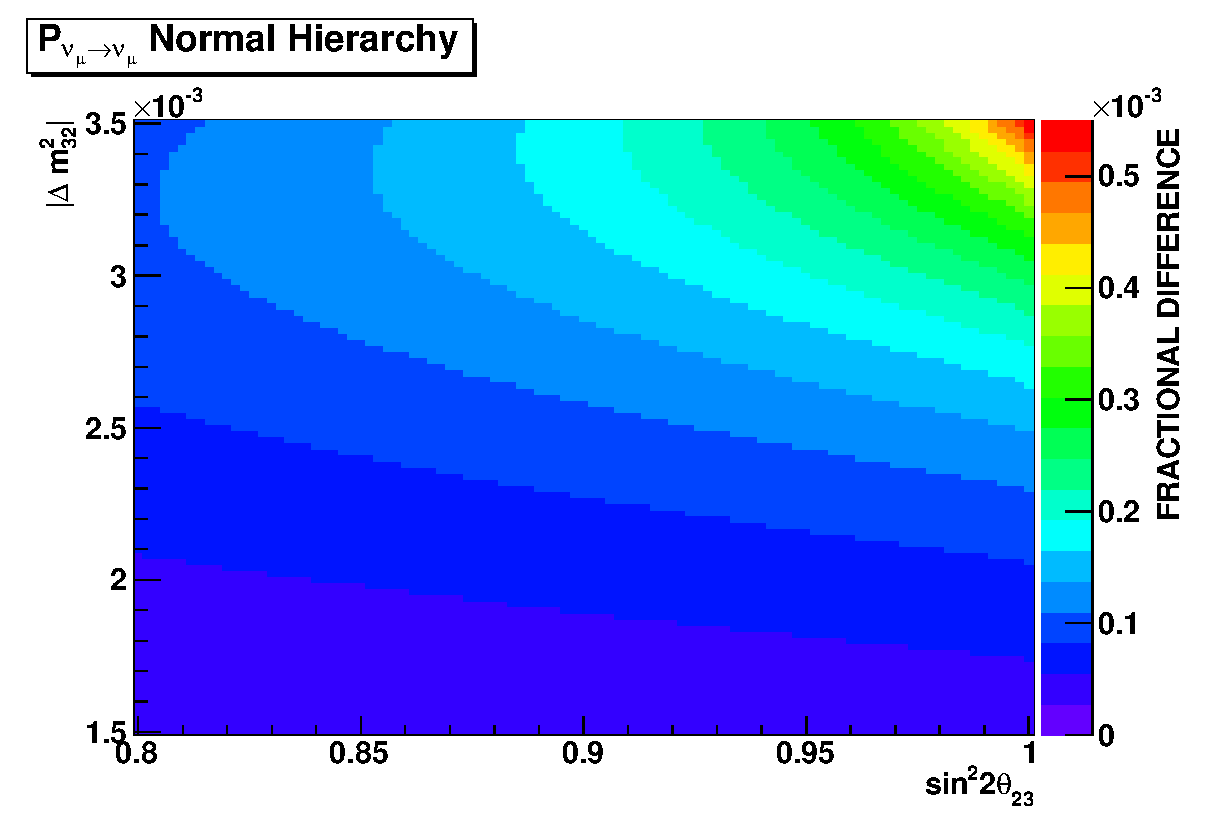
\includegraphics[width=18pc,height=18pc]{./images/osc_prob/prob3_comparison/ComparisonNuMuToNuMuNH.eps}
\caption{
  Comparison of the VaLOR $\nu_{\mu}\rightarrow\nu_{\mu}$ oscillation probabilities in matter with those obtained from Prob3++ 
  as a function of $\sin^{2}2\theta_{23}$ and $|\Delta m_{32}^{2}|$ for E$_{\nu}$ = 1 GeV; normal mass hierarchy, 
  $\sin^{2}2\theta_{13}$ = 0.1, $\sin^{2}2\theta_{12}$ = 0.8704, $\Delta m_{21}^{2}$ = 7.6$\times$10$^{-5}$ eV$^{2}$/c$^{4}$,
  $\delta_{CP}$ = 0 and Earth crust density = 2.6 g/cm$^{3}$.
}
\label{fig:comp_valor_prob3pp_nh_numu_numu}
\end{minipage}
\hspace{0.06\linewidth}
\begin{minipage}[t]{0.48\linewidth}
\centering  
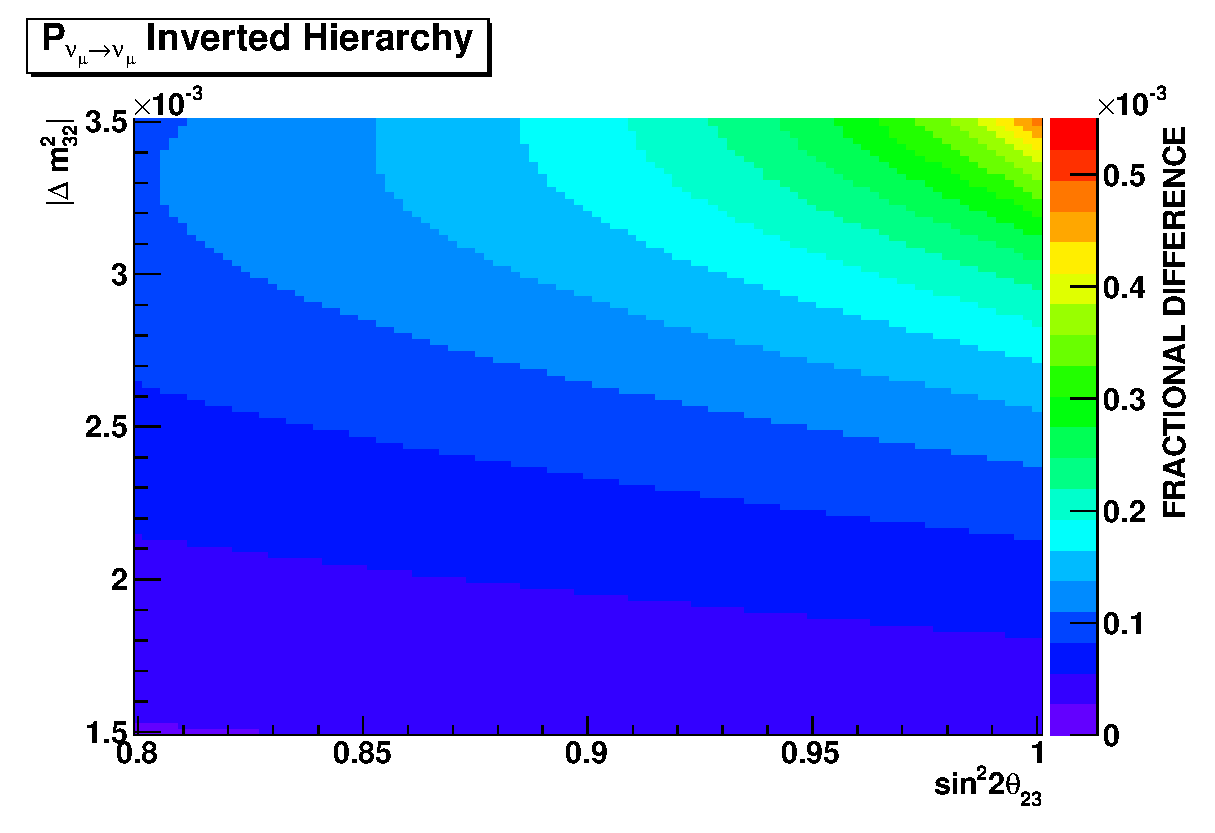
\includegraphics[width=18pc,height=18pc]{./images/osc_prob/prob3_comparison/ComparisonNuMuToNuMuIH.eps}
\caption{
  Comparison of the VaLOR $\nu_{\mu}\rightarrow\nu_{\mu}$ oscillation probabilities in matter with those obtained from Prob3++ 
  as a function of $\sin^{2}2\theta_{23}$ and $|\Delta m_{32}^{2}|$ for E$_{\nu}$ = 1 GeV; inverted mass hierarchy, 
  $\sin^{2}2\theta_{13}$ = 0.1, $\sin^{2}2\theta_{12}$ = 0.8704, $\Delta m_{21}^{2}$ = 7.6$\times$10$^{-5}$ eV$^{2}$/c$^{4}$,
  $\delta_{CP}$ = 0 and Earth crust density = 2.6 g/cm$^{3}$.
}
\label{fig:comp_valor_prob3pp_nh_numu_numu}
\end{minipage}
\end{figure}


%
% numubar -> numubar
%

\begin{figure}[ht]
\begin{minipage}[t]{0.47\linewidth}
\centering
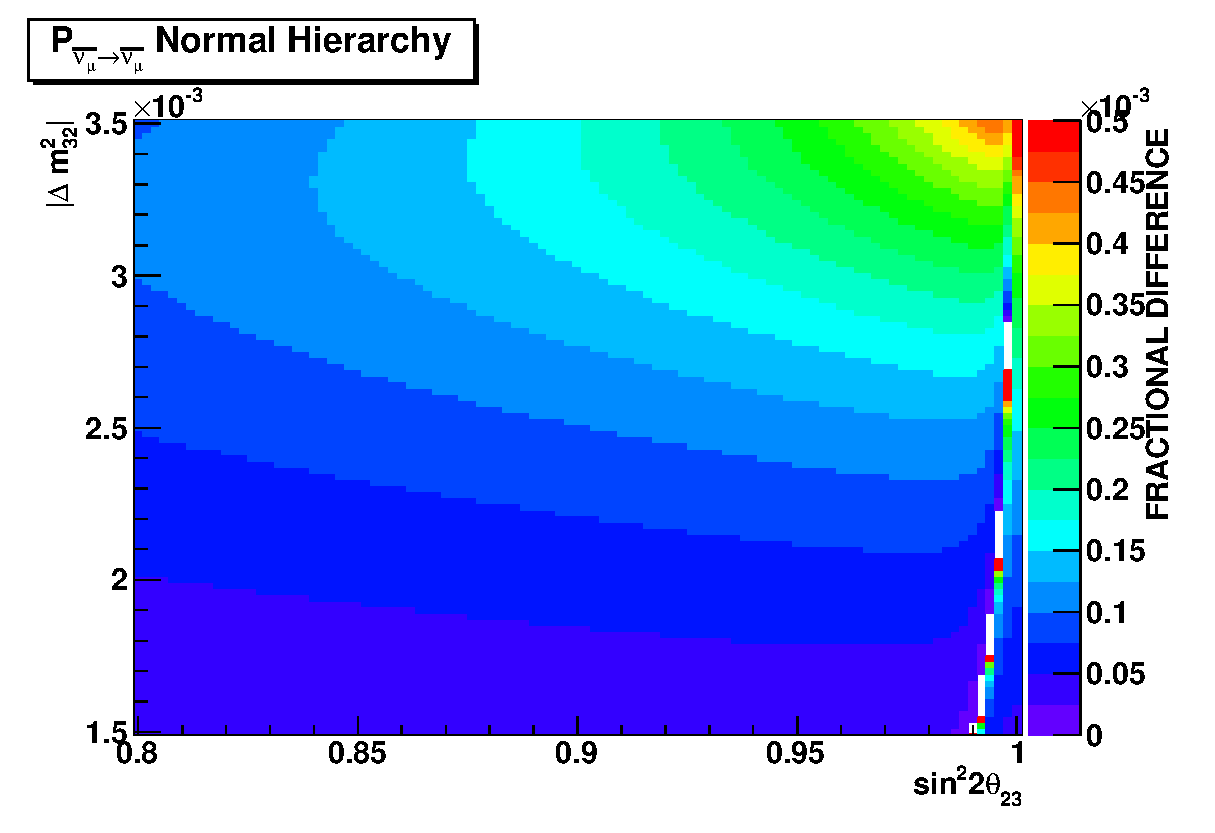
\includegraphics[width=18pc,height=18pc]{./images/osc_prob/prob3_comparison/ComparisonNuMuBarToNuMuBarNH.eps}
\caption{
  Comparison of the VaLOR $\bar{\nu}_{\mu}\rightarrow\bar{\nu}_{\mu}$ oscillation probabilities in matter with those obtained from Prob3++ 
  as a function of $\sin^{2}2\theta_{23}$ and $|\Delta m_{32}^{2}|$ for E$_{\nu}$ = 1 GeV; normal mass hierarchy, 
  $\sin^{2}2\theta_{13}$ = 0.1, $\sin^{2}2\theta_{12}$ = 0.8704, $\Delta m_{21}^{2}$ = 7.6$\times$10$^{-5}$ eV$^{2}$/c$^{4}$,
  $\delta_{CP}$ = 0 and Earth crust density = 2.6 g/cm$^{3}$.
}
\label{fig:comp_valor_prob3pp_nh_numubar_numubar}
\end{minipage}
\hspace{0.06\linewidth}
\begin{minipage}[t]{0.47\linewidth}
\centering  
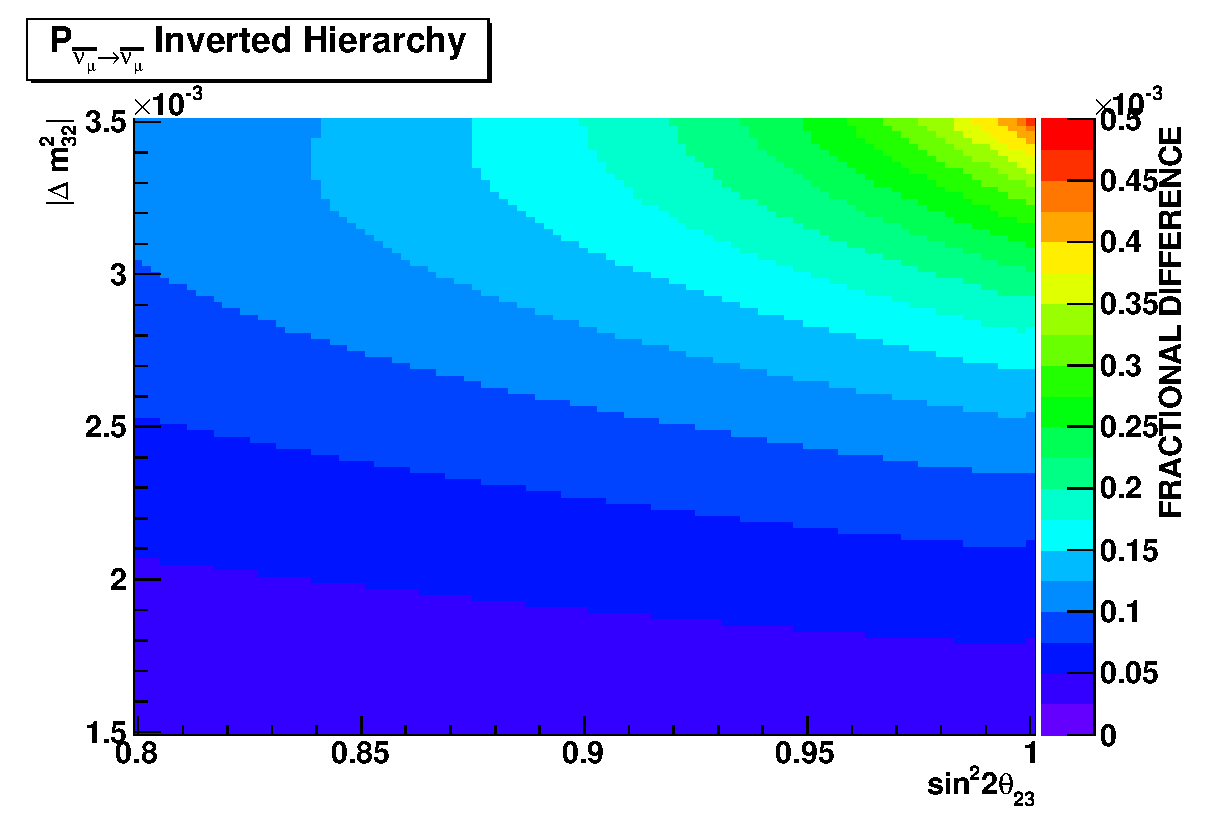
\includegraphics[width=18pc,height=18pc]{./images/osc_prob/prob3_comparison/ComparisonNuMuBarToNuMuBarIH.eps}
\caption{
  Comparison of the VaLOR $\bar{\nu}_{\mu}\rightarrow\bar{\nu}_{\mu}$ oscillation probabilities in matter with those obtained from Prob3++ 
  as a function of $\sin^{2}2\theta_{23}$ and $|\Delta m_{32}^{2}|$ for E$_{\nu}$ = 1 GeV; inverted mass hierarchy, 
  $\sin^{2}2\theta_{13}$ = 0.1, $\sin^{2}2\theta_{12}$ = 0.8704, $\Delta m_{21}^{2}$ = 7.6$\times$10$^{-5}$ eV$^{2}$/c$^{4}$,
  $\delta_{CP}$ = 0 and Earth crust density = 2.6 g/cm$^{3}$.
}
\label{fig:comp_valor_prob3pp_nh_numubar_numubar}
\end{minipage}
\end{figure}


%
% nue -> nue
%

\begin{figure}[ht]
\begin{minipage}[t]{0.47\linewidth}
\centering
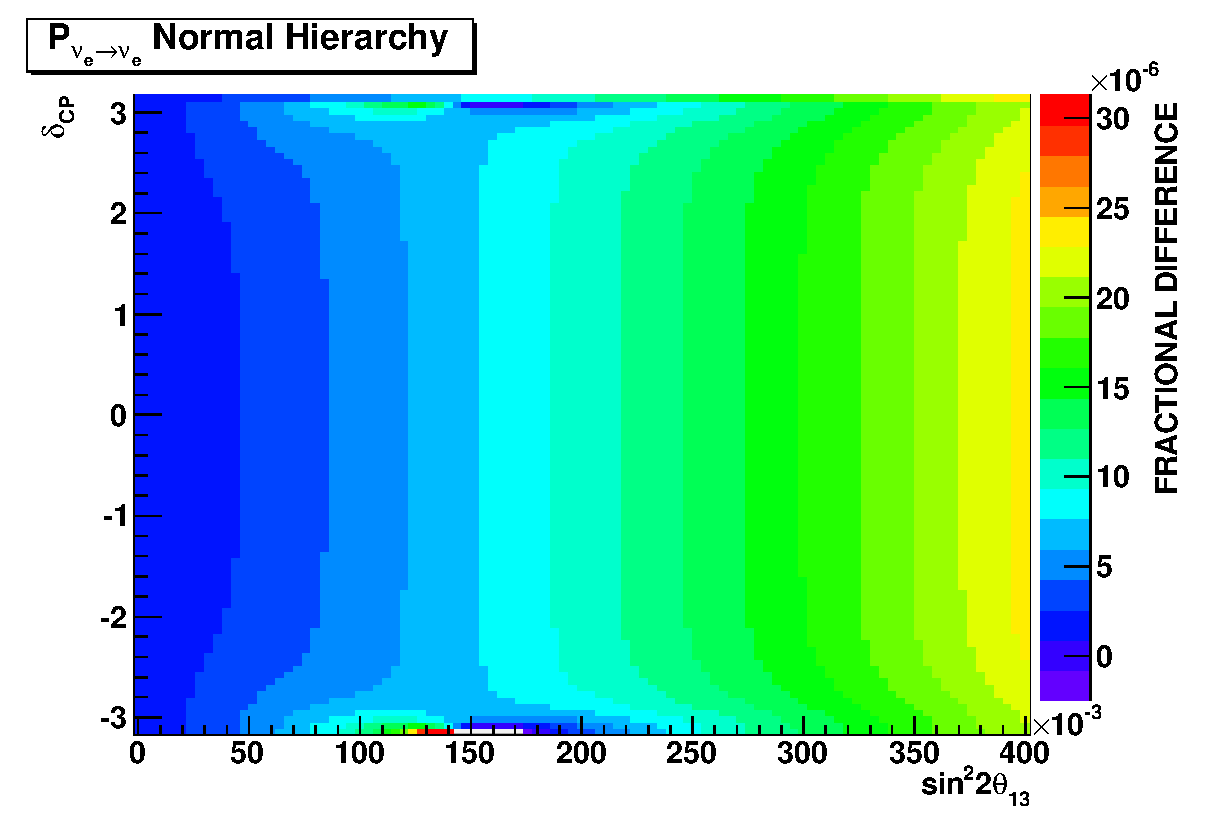
\includegraphics[width=18pc,height=18pc]{./images/osc_prob/prob3_comparison/ComparisonNuEToNuENH.eps}
\caption{
  Comparison of the VaLOR $\nu_{e}\rightarrow\nu_{e}$ oscillation probabilities in matter with those obtained from Prob3++ 
  as a function of $\sin^{2}2\theta_{13}$ and $\delta_{CP}$ for E$_{\nu}$ = 1 GeV; normal mass hierarchy, 
  $\sin^{2}2\theta_{23}$ = 1.0, $|\Delta m_{32}^{2}|$ = 2.4$\times$10$^{-3}$ eV$^{2}$/c$^{4}$, $\sin^{2}2\theta_{12}$ = 0.8704,
  $\Delta m_{21}^{2}$ = 7.6$\times$10$^{-5}$ eV$^{2}$/c$^{4}$ and Earth crust density = 2.6 g/cm$^{3}$.
}
\label{fig:comp_valor_prob3pp_nh_nue_nue}
\end{minipage}
\hspace{0.06\linewidth}
\begin{minipage}[t]{0.47\linewidth}
\centering  
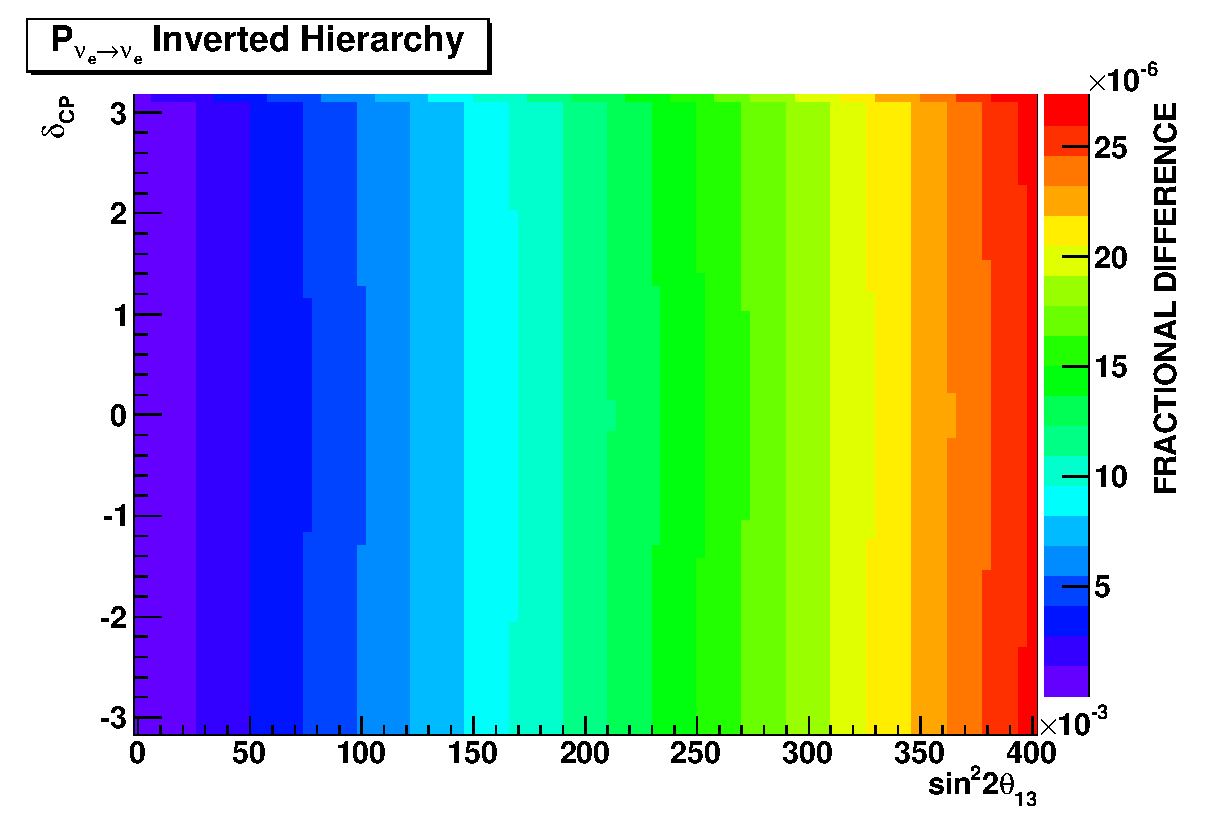
\includegraphics[width=18pc,height=18pc]{./images/osc_prob/prob3_comparison/ComparisonNuEToNuEIH.eps}
\caption{
  Comparison of the VaLOR $\nu_{e}\rightarrow\nu_{e}$ oscillation probabilities in matter with those obtained from Prob3++ 
  as a function of $\sin^{2}2\theta_{13}$ and $\delta_{CP}$ for E$_{\nu}$ = 1 GeV; inverted mass hierarchy, 
  $\sin^{2}2\theta_{23}$ = 1.0, $|\Delta m_{32}^{2}|$ = 2.4$\times$10$^{-3}$ eV$^{2}$/c$^{4}$, $\sin^{2}2\theta_{12}$ = 0.8704,
  $\Delta m_{21}^{2}$ = 7.6$\times$10$^{-5}$ eV$^{2}$/c$^{4}$ and Earth crust density = 2.6 g/cm$^{3}$.
}
\label{fig:comp_valor_prob3pp_nh_nue_nue}
\end{minipage}
\end{figure}


%
% nuebar -> nuebar
%

\begin{figure}[ht]
\begin{minipage}[t]{0.47\linewidth}
\centering
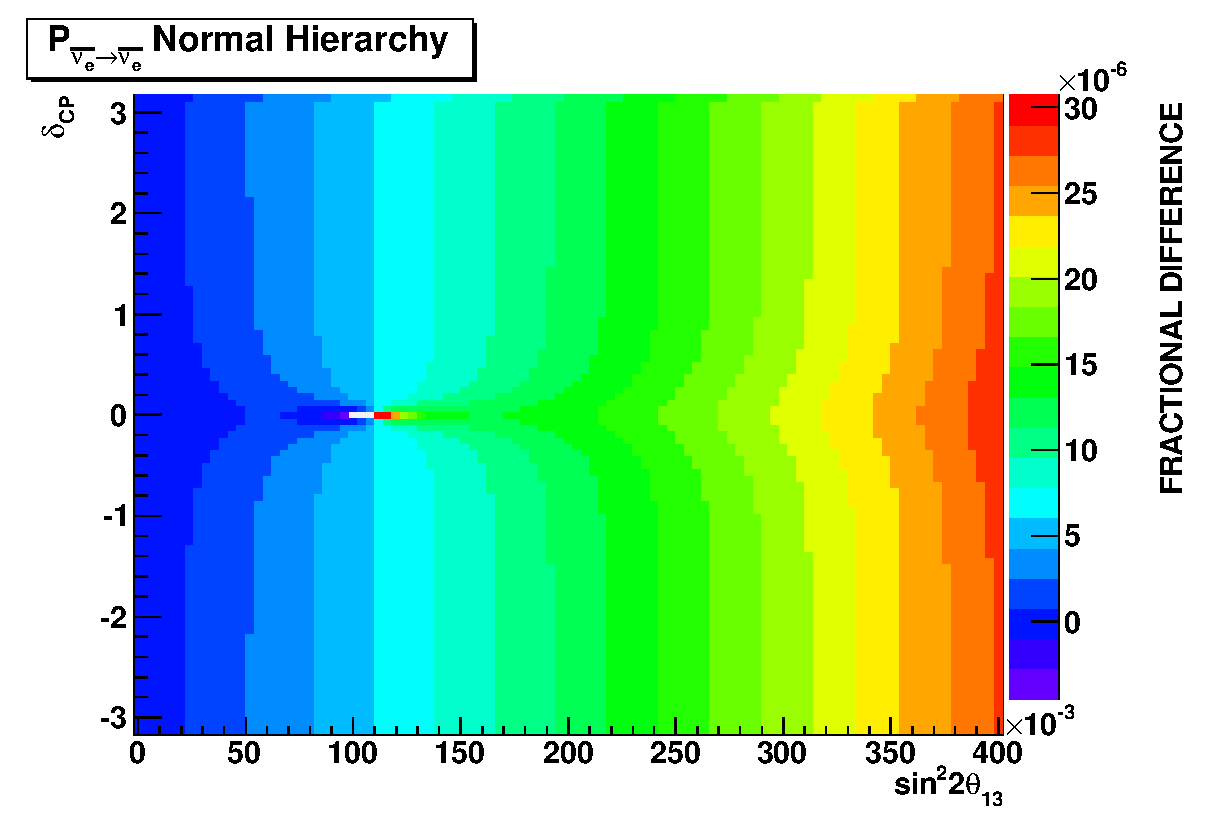
\includegraphics[width=18pc,height=18pc]{./images/osc_prob/prob3_comparison/ComparisonNuEBarToNuEBarNH.eps}
\caption{
  Comparison of the VaLOR $\bar{\nu}_{e}\rightarrow\bar{\nu}_{e}$ oscillation probabilities in matter with those obtained from Prob3++ 
  as a function of $\sin^{2}2\theta_{13}$ and $\delta_{CP}$ for E$_{\nu}$ = 1 GeV; normal mass hierarchy, 
  $\sin^{2}2\theta_{23}$ = 1.0, $|\Delta m_{32}^{2}|$ = 2.4$\times$10$^{-3}$ eV$^{2}$/c$^{4}$, $\sin^{2}2\theta_{12}$ = 0.8704,
  $\Delta m_{21}^{2}$ = 7.6$\times$10$^{-5}$ eV$^{2}$/c$^{4}$ and Earth crust density = 2.6 g/cm$^{3}$.
}
\label{fig:comp_valor_prob3pp_nh_nuebar_nuebar}
\end{minipage}
\hspace{0.06\linewidth}
\begin{minipage}[t]{0.47\linewidth}
\centering  
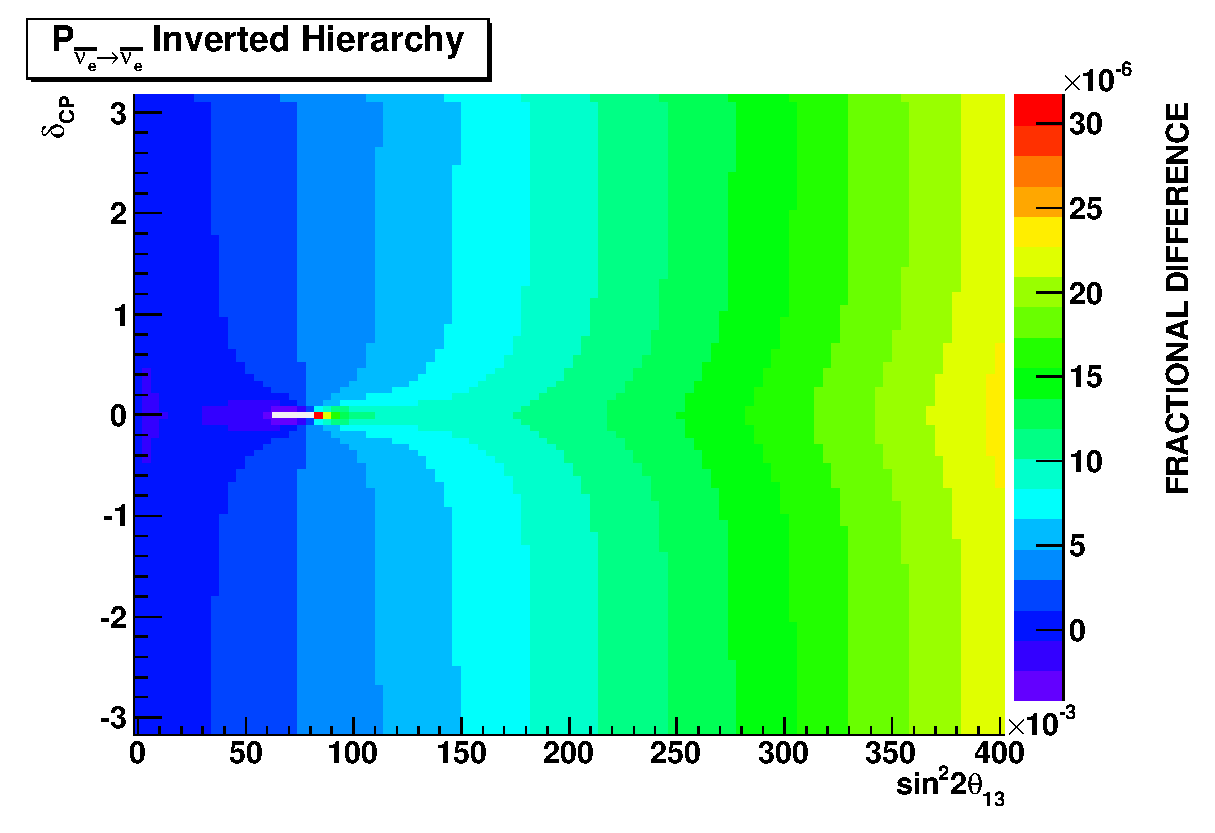
\includegraphics[width=18pc,height=18pc]{./images/osc_prob/prob3_comparison/ComparisonNuEBarToNuEBarIH.eps}
\caption{
  Comparison of the VaLOR $\bar{\nu}_{e}\rightarrow\bar{\nu}_{e}$ oscillation probabilities in matter with those obtained from Prob3++ 
  as a function of $\sin^{2}2\theta_{13}$ and $\delta_{CP}$ for E$_{\nu}$ = 1 GeV; inverted mass hierarchy, 
  $\sin^{2}2\theta_{23}$ = 1.0, $|\Delta m_{32}^{2}|$ = 2.4$\times$10$^{-3}$ eV$^{2}$/c$^{4}$, $\sin^{2}2\theta_{12}$ = 0.8704,
  $\Delta m_{21}^{2}$ = 7.6$\times$10$^{-5}$ eV$^{2}$/c$^{4}$ and Earth crust density = 2.6 g/cm$^{3}$.
}
\label{fig:comp_valor_prob3pp_nh_nuebar_nuebar}
\end{minipage}
\end{figure}

%
% numu -> nue
%

\begin{figure}[ht]
\begin{minipage}[t]{0.47\linewidth}
\centering
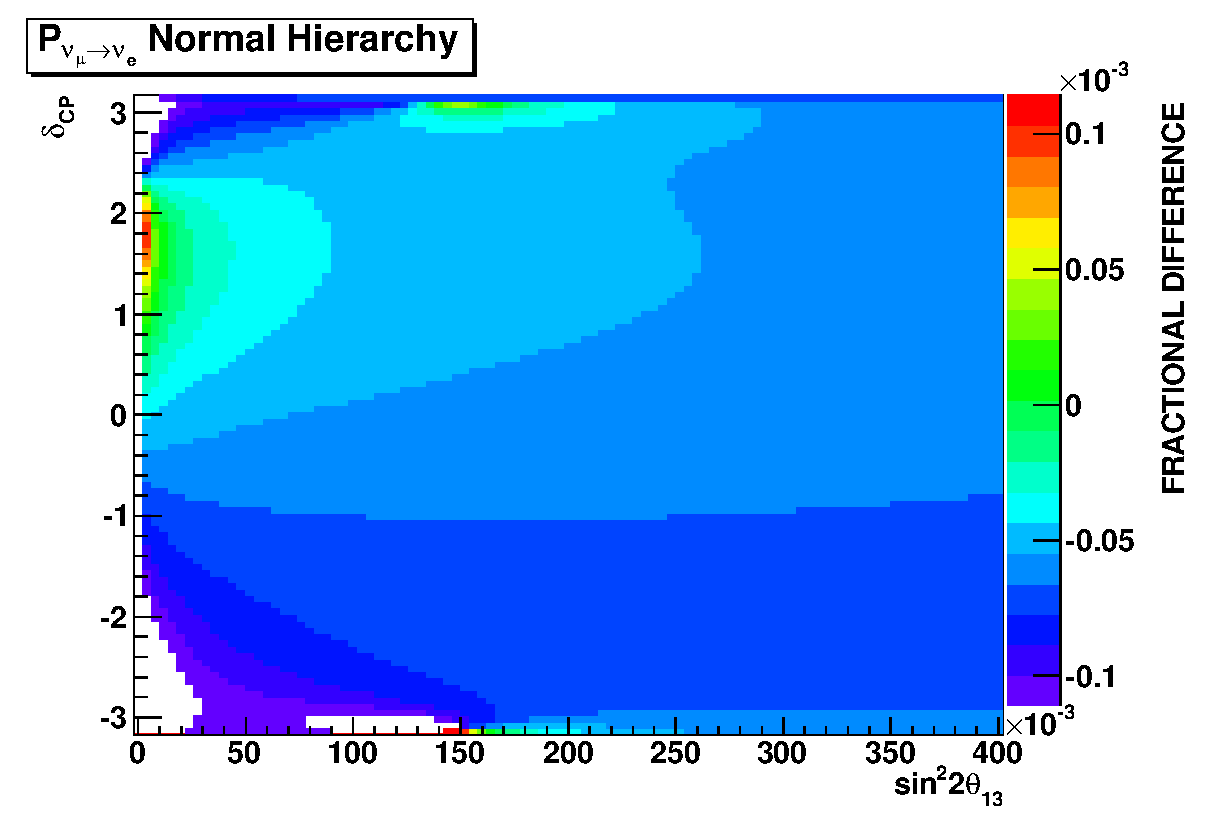
\includegraphics[width=18pc,height=18pc]{./images/osc_prob/prob3_comparison/ComparisonNuMuToNuENH.eps}
\caption{
  Comparison of the VaLOR $\nu_{\mu}\rightarrow\nu_{e}$ oscillation probabilities in matter with those obtained from Prob3++ 
  as a function of $\sin^{2}2\theta_{13}$ and $\delta_{CP}$ for E$_{\nu}$ = 1 GeV; normal mass hierarchy, 
  $\sin^{2}2\theta_{23}$ = 1.0, $|\Delta m_{32}^{2}|$ = 2.4$\times$10$^{-3}$ eV$^{2}$/c$^{4}$, $\sin^{2}2\theta_{12}$ = 0.8704,
  $\Delta m_{21}^{2}$ = 7.6$\times$10$^{-5}$ eV$^{2}$/c$^{4}$ and Earth crust density = 2.6 g/cm$^{3}$.
}
\label{fig:comp_valor_prob3pp_nh_numu_nue}
\end{minipage}
\hspace{0.06\linewidth}
\begin{minipage}[t]{0.47\linewidth}
\centering  
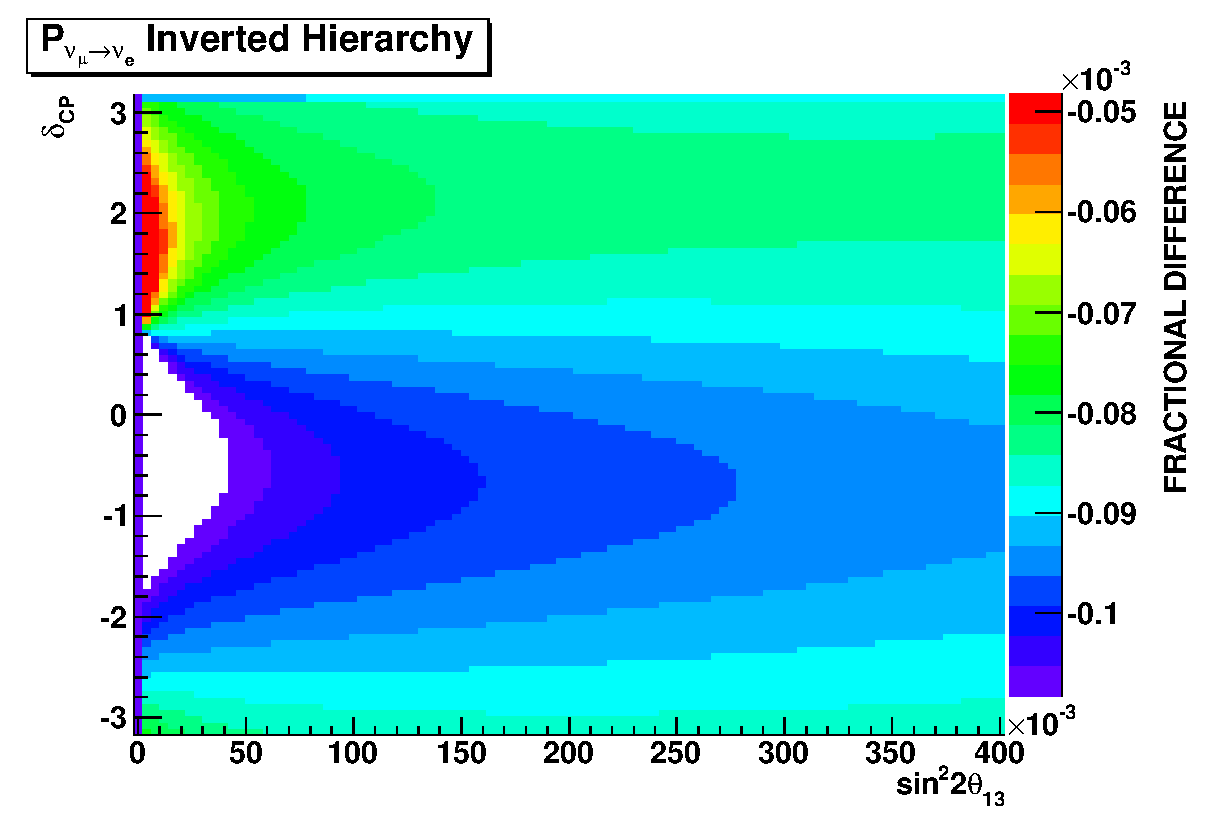
\includegraphics[width=18pc,height=18pc]{./images/osc_prob/prob3_comparison/ComparisonNuMuToNuEIH.eps}
\caption{
  Comparison of the VaLOR $\nu_{\mu}\rightarrow\nu_{e}$ oscillation probabilities in matter with those obtained from Prob3++ 
  as a function of $\sin^{2}2\theta_{13}$ and $\delta_{CP}$ for E$_{\nu}$ = 1 GeV; inverted mass hierarchy, 
  $\sin^{2}2\theta_{23}$ = 1.0, $|\Delta m_{32}^{2}|$ = 2.4$\times$10$^{-3}$ eV$^{2}$/c$^{4}$, $\sin^{2}2\theta_{12}$ = 0.8704, 
  $\Delta m_{21}^{2}$ = 7.6$\times$10$^{-5}$ eV$^{2}$/c$^{4}$ and Earth crust density = 2.6 g/cm$^{3}$.
}
\label{fig:comp_valor_prob3pp_nh_numu_nue}
\end{minipage}
\end{figure}

%
% nue -> numu
%

\begin{figure}[ht]
\begin{minipage}[t]{0.47\linewidth}
\centering
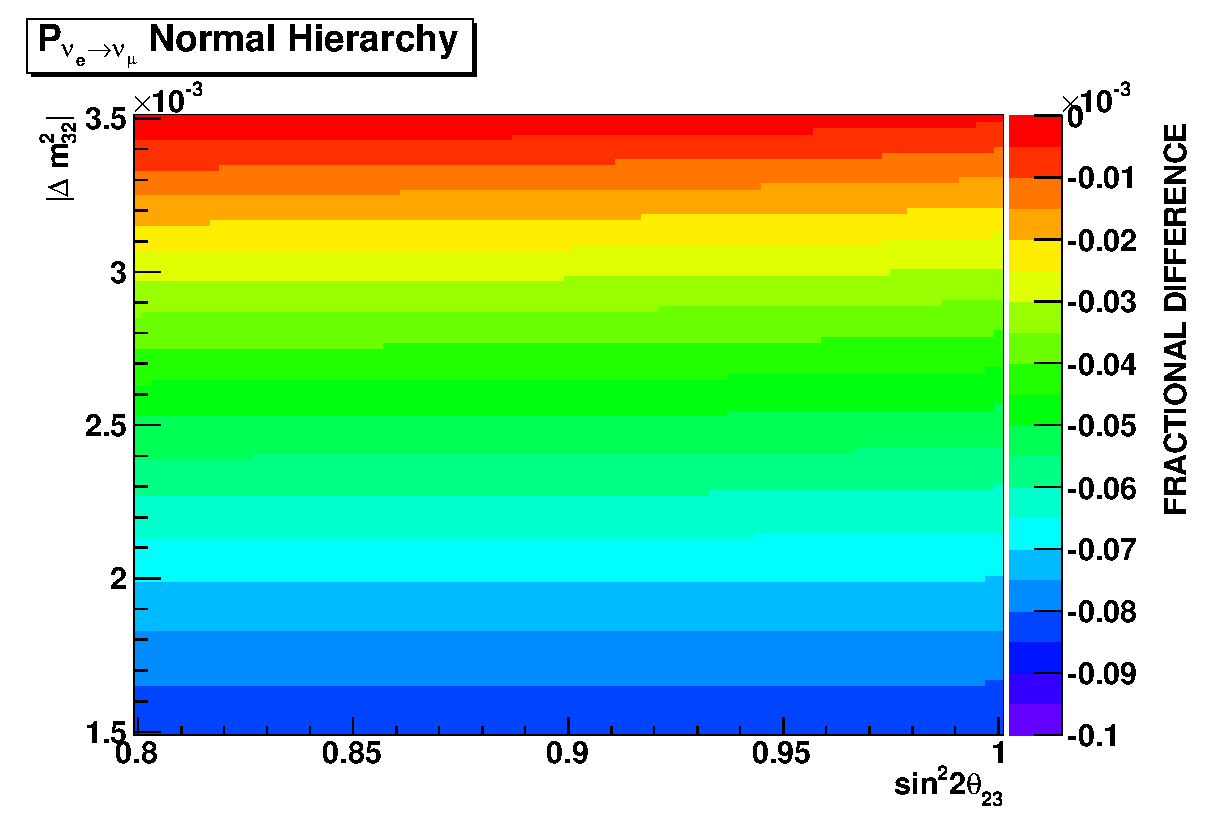
\includegraphics[width=18pc,height=18pc]{./images/osc_prob/prob3_comparison/ComparisonNuEToNuMuNH.eps}
\caption{
  Comparison of the VaLOR $\nu_{e}\rightarrow\nu_{\mu}$ oscillation probabilities in matter with those obtained from Prob3++ 
  as a function of $\sin^{2}2\theta_{23}$ and $|\Delta m_{32}^{2}|$ for E$_{\nu}$ = 1 GeV; normal mass hierarchy, 
  $\sin^{2}2\theta_{13}$ = 0.1, $\sin^{2}2\theta_{12}$ = 0.8704, $\Delta m_{21}^{2}$ = 7.6$\times$10$^{-5}$ eV$^{2}$/c$^{4}$,
  $\delta_{CP}$ = 0 and Earth crust density = 2.6 g/cm$^{3}$.
}
\label{fig:comp_valor_prob3pp_nh_nue_numu}
\end{minipage}
\hspace{0.06\linewidth}
\begin{minipage}[t]{0.47\linewidth}
\centering  
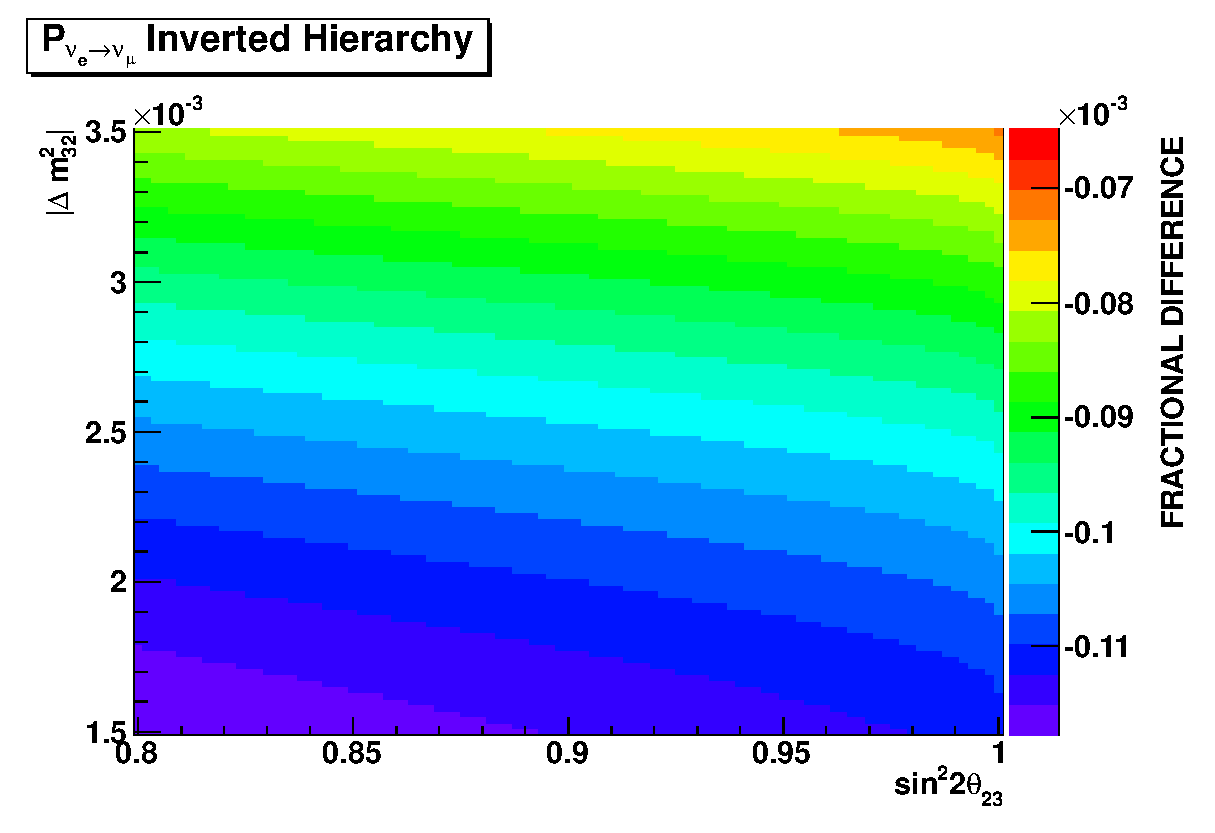
\includegraphics[width=18pc,height=18pc]{./images/osc_prob/prob3_comparison/ComparisonNuEToNuMuIH.eps}
\caption{
  Comparison of the VaLOR $\nu_{e}\rightarrow\nu_{\mu}$ oscillation probabilities in matter with those obtained from Prob3++ 
  as a function of $\sin^{2}2\theta_{23}$ and $|\Delta m_{32}^{2}|$ for E$_{\nu}$ = 1 GeV; inverted mass hierarchy, 
  $\sin^{2}2\theta_{13}$ = 0.1, $\sin^{2}2\theta_{12}$ = 0.8704, $\Delta m_{21}^{2}$ = 7.6$\times$10$^{-5}$ eV$^{2}$/c$^{4}$, 
  $\delta_{CP}$ = 0 and Earth crust density = 2.6 g/cm$^{3}$.
}
\label{fig:comp_valor_prob3pp_nh_nue_numu}
\end{minipage}
\end{figure}



\clearpage

\section {Sensitivity study for the 3.010$\times10^{20}$ POT $\nu_{\mu}$-disappearance analysis}
\label{appendix:sensitivity_study}

A sensitivity study was performed at various points around the MINOS 2012 best-fit values \cite{MINOS2012}.
%(sin$^22\theta_{23}$ = 0.957, $\Delta m_{32}^2$ = 2.39$\times$10$^{-3}$ $eV^{2}/c^{4}$) 
These points are shown in Fig.\ \ref{fig:sensitivity_study_points}, and have the following values of sin$^22\theta_{23}$:
\begin{enumerate}  
\item 1.0 (maximal) 
\item 0.957 (2012 MINOS best-fit value)
\item 0.877 (smallest value in the 2012 MINOS 90\% confidence region)
\end{enumerate}
The sensitivity study points have the following values of $\Delta m_{32}^2$:
\begin{enumerate}
\item 2.09$\times$10$^{-3}$ $eV^{2}/c^{4}$ (2012 MINOS  best-fit value - 3$\sigma$),
\item 2.29$\times$10$^{-3}$ $eV^{2}/c^{4}$ (2012 MINOS  best-fit value - 1$\sigma$),
\item 2.39$\times$10$^{-3}$ $eV^{2}/c^{4}$ (2012 MINOS  best-fit value),
\item 2.48$\times$10$^{-3}$ $eV^{2}/c^{4}$ (2012 MINOS  best-fit value + 1$\sigma$),
\item 2.66$\times$10$^{-3}$ $eV^{2}/c^{4}$ (2012 MINOS  best-fit value + 3$\sigma$).
\end{enumerate}

%
%The following points in sin$^22\theta_{23}$, $\Delta m_{32}^2$ have been studied:
%\begin{itemize}
%\item 1.000, 0.00209;
%\item 1.000, 0.00229;
%\item 1.000, 0.00239;
%\item 1.000, 0.00248;
%\item 1.000, 0.00266;
%\item 0.957, 0.00209;
%\item 0.957, 0.00229;
%\item 0.957, 0.00239;
%\item 0.957, 0.00248;
%\item 0.957, 0.00266;
%\item 0.877, 0.00209;
%\item 0.877, 0.00229;
%\item 0.877, 0.00239;
%\item 0.877, 0.00248;
%\item 0.877, 0.00266.
%\end{itemize}
%

\begin{figure*}[htb]
\center
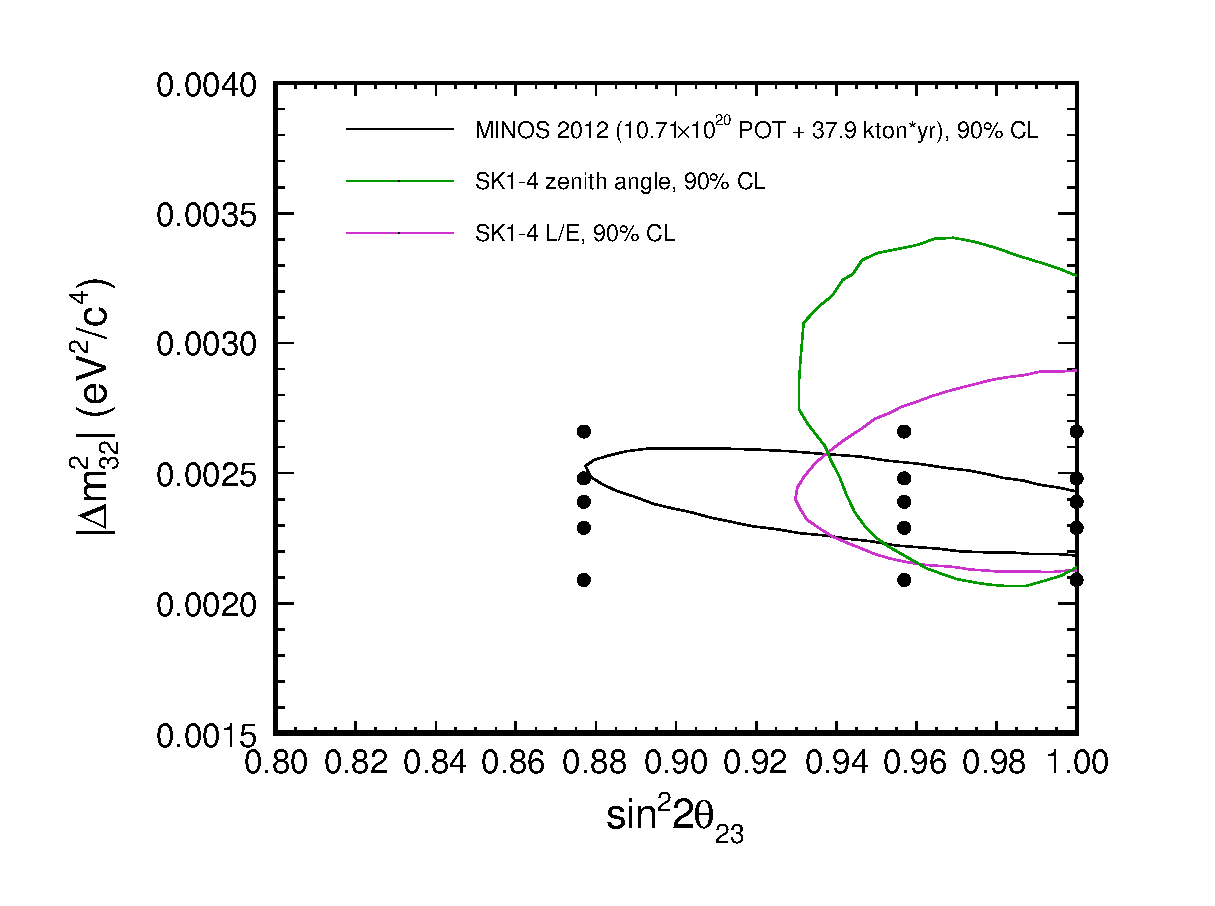
\includegraphics[width=35pc]{./images/sensitivities/sensitivity_study_points.eps}
\caption {
 True oscillation parameters points considered in our T2K sensitivity study.
 The grid was constructed using the 2012 MINOS best-fit $\Delta m_{32}^2$ value 
 and $\pm$1$\sigma$, $\pm$3$\sigma$ variations, and using 
 sin$^22\theta_{23}$ values
 of 1 (maximal), 0.957 (2012 MINOS best-fit value) and 0.877 (smallest value in the 2012 MINOS 90\% confidence region).
}
\label{fig:sensitivity_study_points}
\end{figure*}

An average $\chi^2$ surface was constructed as a function of sin$^22\theta_{23}$ and $\Delta m_{32}^2$ by averaging the 
$\chi^2$ surfaces obtained by `2+8' fits to 1K toy MC experiments. In each of these toy experiments, the systematic 
parameters were randomized and statistical fluctuations were included. The confidence contours were then drawn using 
the constant-$\Delta\chi^{2}$ method as described in Sec.\ \ref{sec:contour_construction_constdchi}.

%The $\Delta\chi^2$ surface was then constructed as
%$\Delta\chi^2$ = $\chi^2_{mean}$ - $min(\chi^2_{mean}$)

The results of the sensitivity study are shown in 
Figs. \ref{fig:sensitivity:2+8constdchisq:0.00209}-\ref{fig:sensitivity:2+8constdchisq:0.00266}.

%...........................................
%
%
\begin{figure*}[htb]
\begin{minipage}[t]{0.48\linewidth}
\center
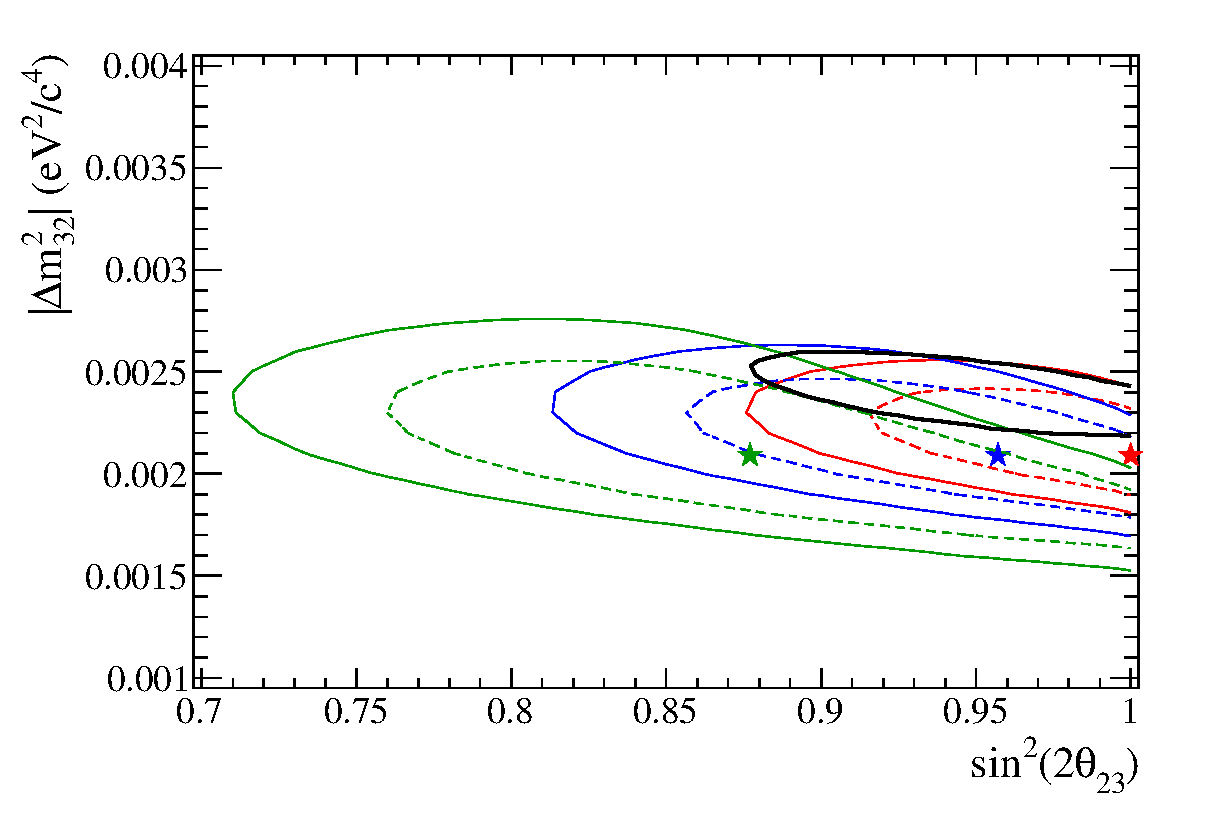
\includegraphics[width=18pc]{./images/sensitivities/2+8constdchisq/sensitivity_1}
\caption {
  T2K 68\% CL and 90\% CL sensitivity contours, for $3.010 \times 10^{20}$ POT, computed using the `2+8' fit.
  The input (sin$^22\theta_{23}$, $\Delta m_{32}^2$ (in $eV^{2}/c^{4}$)) points
  shown in red, blue and green are, respectively,
  (1.000, 0.00209), 
  (0.957, 0.00209), 
  (0.877, 0.00209).
  The 2012 MINOS 90\% CL region is shown in black.
}
\label{fig:sensitivity:2+8constdchisq:0.00209}
\end{minipage}
\hspace{0.06\linewidth}
\begin{minipage}[t]{0.48\linewidth}
\center
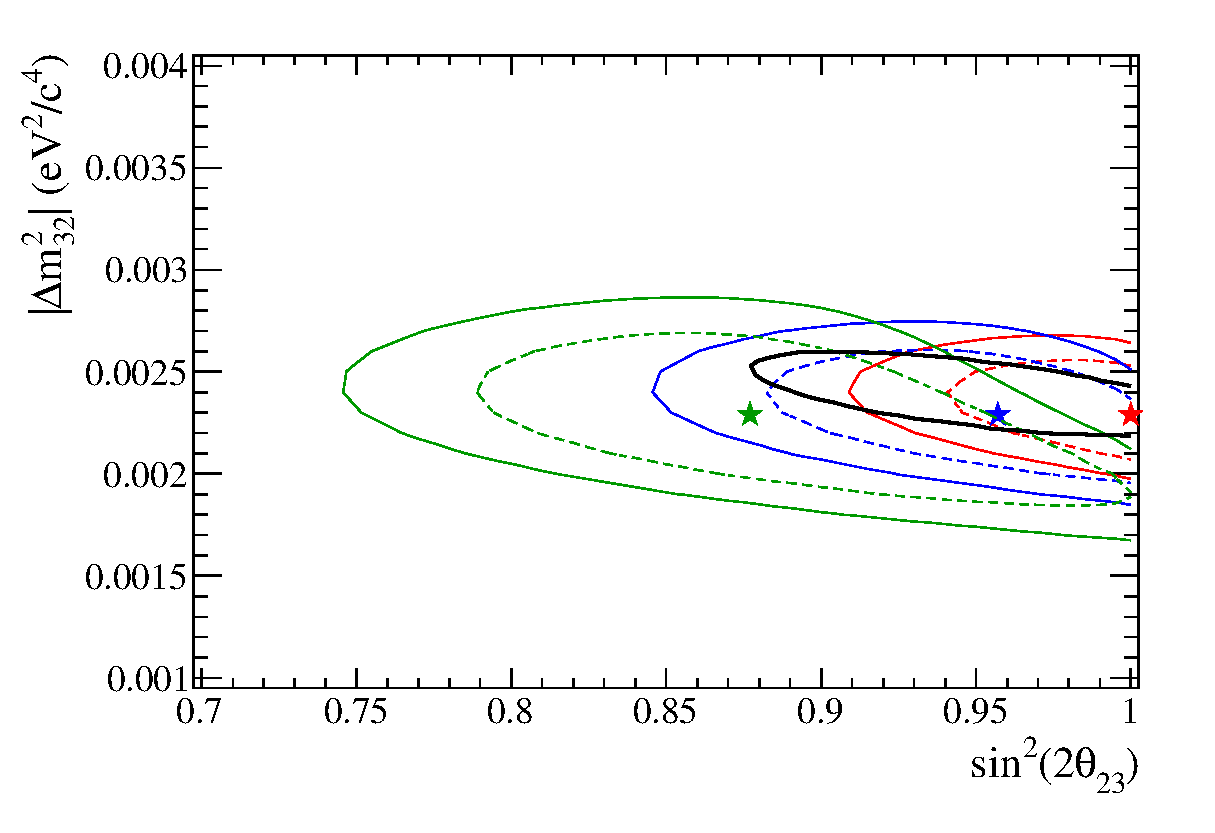
\includegraphics[width=18pc]{./images/sensitivities/2+8constdchisq/sensitivity_2}
\caption {
  T2K 68\% CL and 90\% CL sensitivity contours, for $3.010 \times 10^{20}$ POT, computed using the `2+8' fit.
  The input (sin$^22\theta_{23}$, $\Delta m_{32}^2$ (in $eV^{2}/c^{4}$)) points 
  shown in red, blue and green are, respectively,
  (1.000, 0.00229), 
  (0.957, 0.00229), 
  (0.877, 0.00229).
  The 2012 MINOS 90\% CL region is shown in black.
}
\label{fig:sensitivity:2+8constdchisq:0.00229}
\end{minipage}
\end{figure*}


\begin{figure*}[htb]
\begin{minipage}[t]{0.48\linewidth}
\center
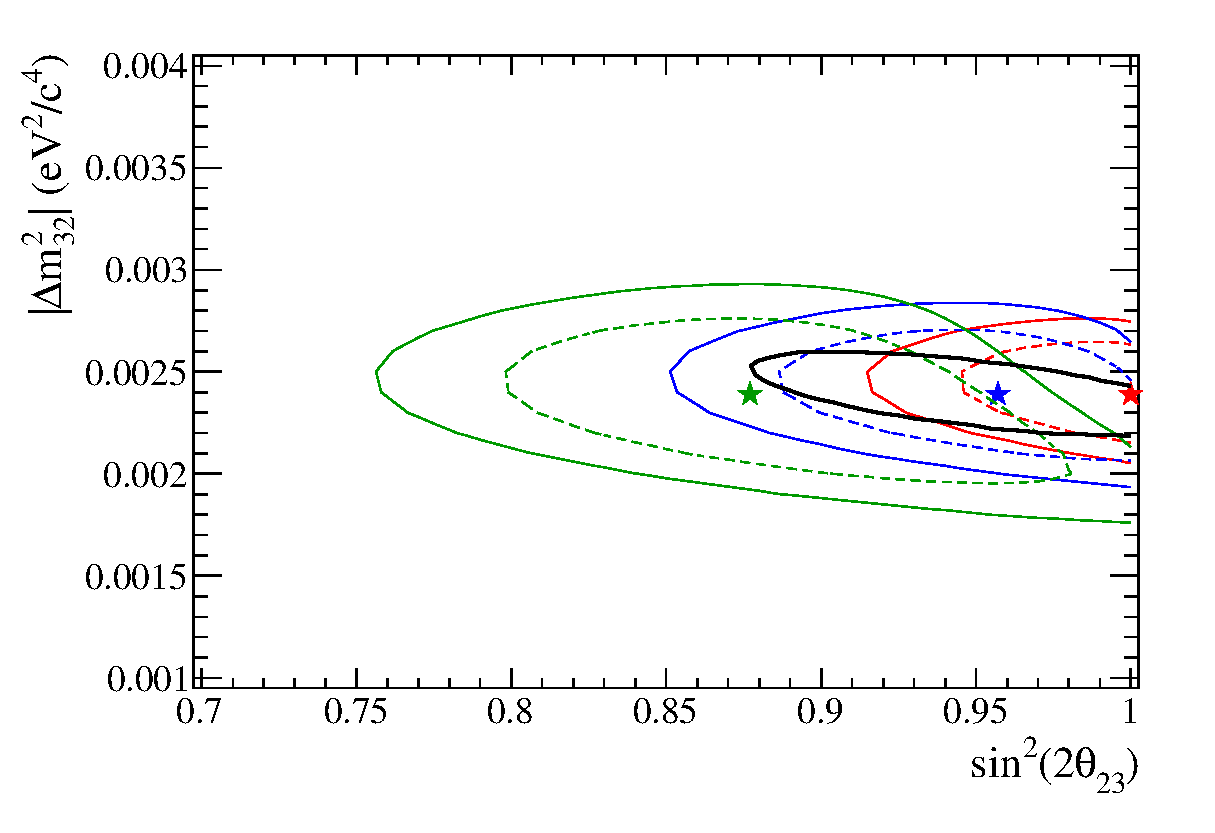
\includegraphics[width=18pc]{./images/sensitivities/2+8constdchisq/sensitivity_3}
\caption {
  T2K 68\% CL and 90\% CL sensitivity contours, for $3.010 \times 10^{20}$ POT, computed using the `2+8' fit.
  The input (sin$^22\theta_{23}$, $\Delta m_{32}^2$ (in $eV^{2}/c^{4}$)) points 
  shown in red, blue and green are, respectively,
  (1.000, 0.00239), 
  (0.957, 0.00239), 
  (0.877, 0.00239).
  The 2012 MINOS 90\% CL region is shown in black.
}
\label{fig:sensitivity:2+8constdchisq:0.00239}
\end{minipage}
\hspace{0.06\linewidth}
\begin{minipage}[t]{0.48\linewidth}
\center
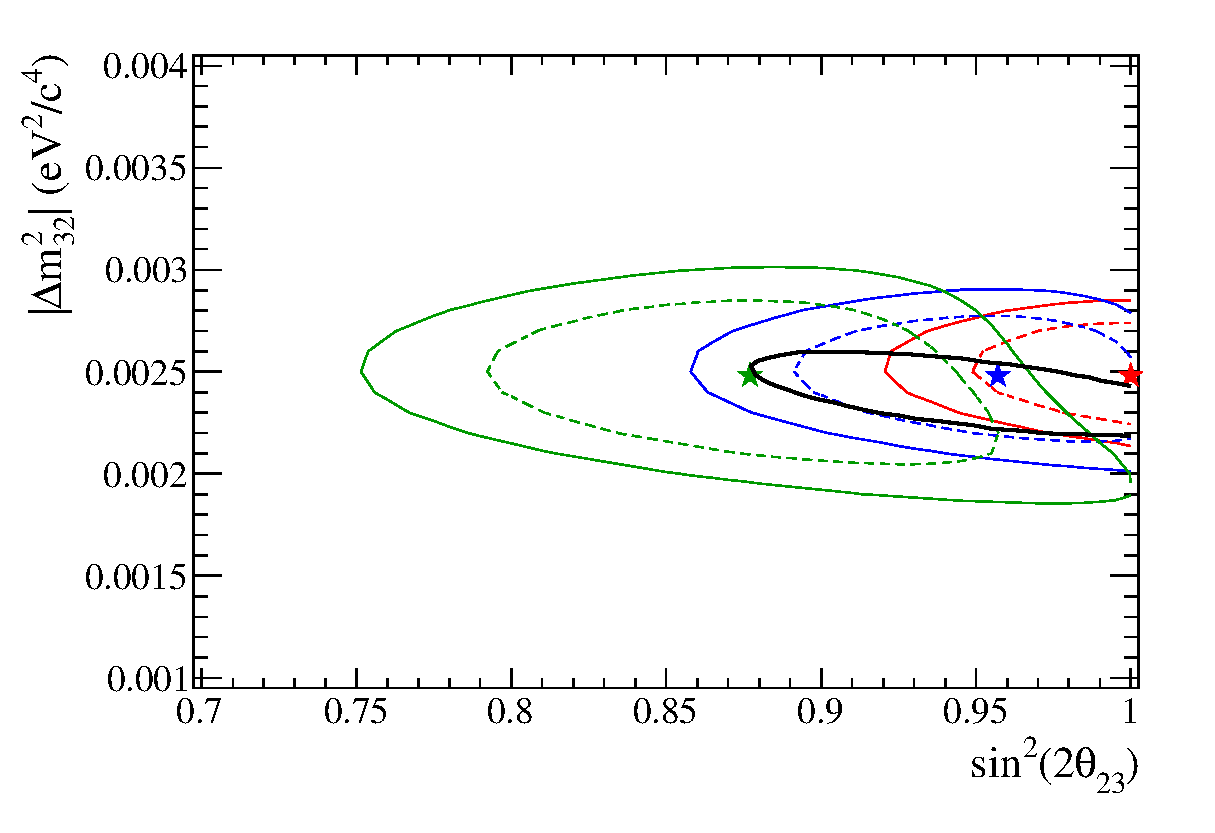
\includegraphics[width=18pc]{./images/sensitivities/2+8constdchisq/sensitivity_4}
\caption {
  T2K 68\% CL and 90\% CL sensitivity contours, for $3.010 \times 10^{20}$ POT, computed using the `2+8' fit.
  The input (sin$^22\theta_{23}$, $\Delta m_{32}^2$ (in $eV^{2}/c^{4}$)) points 
  shown in red, blue and green are, respectively,
  (1.000, 0.00248), 
  (0.957, 0.00248), 
  (0.877, 0.00248).
  The 2012 MINOS 90\% CL region is shown in black.
}
\label{fig:sensitivity:2+8constdchisq:0.00248}
\end{minipage}
\end{figure*}


\begin{figure*}[htb]
\begin{minipage}[t]{0.48\linewidth}
\center
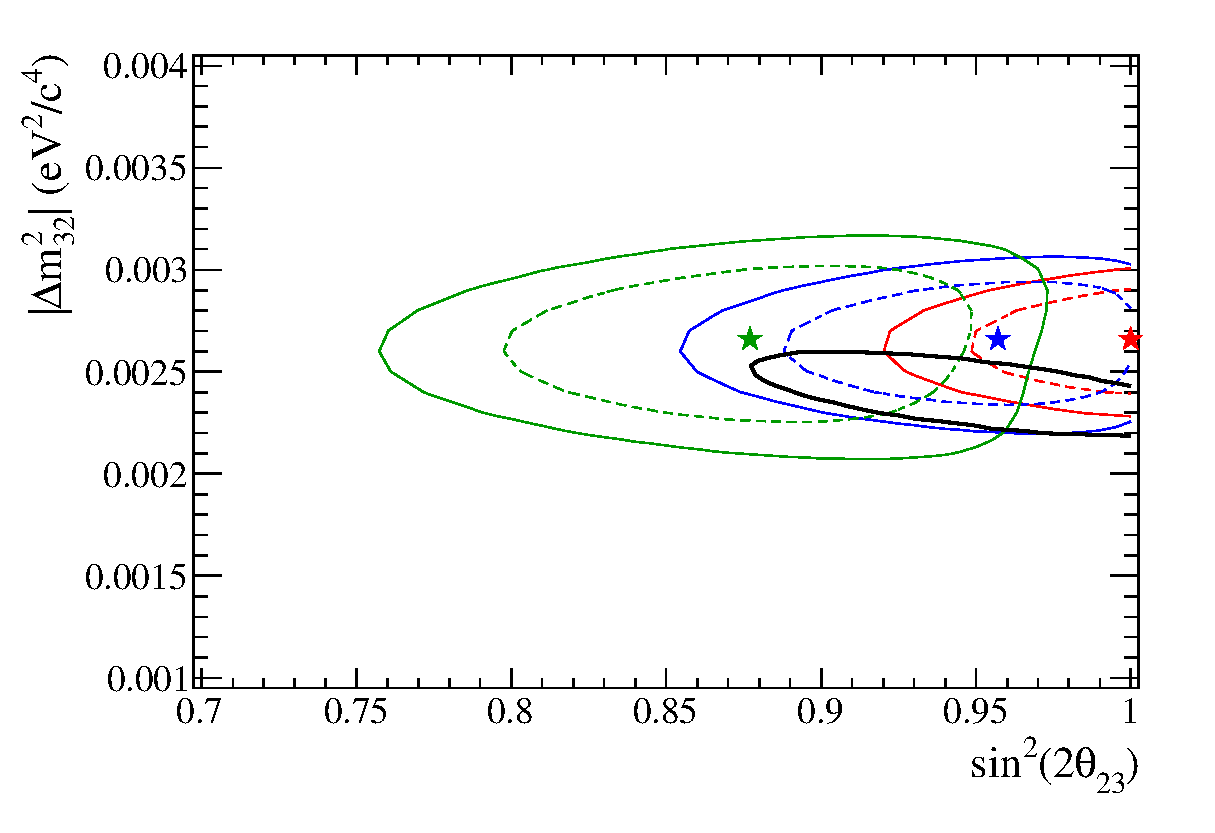
\includegraphics[width=18pc]{./images/sensitivities/2+8constdchisq/sensitivity_0}
\caption {
  T2K 68\% CL and 90\% CL sensitivity contours, for $3.010 \times 10^{20}$ POT, computed using the `2+8' fit.
  The input (sin$^22\theta_{23}$, $\Delta m_{32}^2$ (in $eV^{2}/c^{4}$)) points 
  shown in red, blue and green are, respectively,
  (1.000, 0.00266), 
  (0.957, 0.00266),  
  (0.877, 0.00266).
  The 2012 MINOS 90\% CL region is also shown in black.
}
\label{fig:sensitivity:2+8constdchisq:0.00266}
\end{minipage}
\end{figure*}

\clearpage

\section{Example toy MC fits}
\label{appendix:example_toy_mc_fits}

Six toy MC SuperK datasets were created with a POT corresponding to the Run 1+2+3 data; two
datasets were created by each of the KIT, VaLOR and MuSiC groups. Each dataset included random variations of all
of the systematic parameters, with these variations and the true oscillation parameters being unknown to the analysers
in the groups that did not create the datasets. Each dataset was fitted using both a 2+8 and a 2+N fit, and the value 
of chisq (from equation \ref{eq:chisquare}) was obtained at the best-fit point for each fit. All these fits were made 
with the coarse binning scheme discussed in Sec.\ref{sec:gof_test}.

Goodness-of-fit tests were carried out on these six toy datasets. 
The best-fit values of $\sin^{2}2\theta_{23}$ and $\Delta m^{2}_{32}$ obtained in the 5-bin fit to the first dataset
were then used as input true oscillation parameters to create 1000 additional toy MC datasets. Both statistical and
systematic variations were included in these additional datasets. Each additional dataset was fitted using a 5-bin
2+8 fit to find the value of chisq at the best-fit point. The p-value for the first of the original datasets was
then calculated as the ratio of the number of additional datasets whose best-fit chisq was greater than that of the
original dataset to the total number of additional datasets. This calculation of the p-value was then repeated for 
each of the other 5 original datasets. 

\begin{table}[b]
\centering
\begin{tabular}{| c | c | c  c | c  c  c | l |}
\hline
Fake data set & Analysis & sin$^22\theta_{23}$ & $|\Delta m_{32}^2|$ (eV$^{2}$/c$^{4}$) & N$_{SK}$ & $\chi^2_{bestfit}$/ndf & Systematics \\
\hline
  &       & {\bf 1.000} & {\bf 2.250$\times$10$^{-3}$} & {\bf 63} & - & {\bf Nominal} \\
0 & `2+N' & 1.000 & 2.130$\times$10$^{-3}$ & 66.09  & 82.30/71  & See Fig. \ref{fig:fakedata_pulls_2N_0} \\
  & `2+8' & 1.000 & 2.133$\times$10$^{-3}$ & 65.88 & 82.45/71   & See Fig. \ref{fig:fakedata_pulls_0} \\
\hline
  &       & {\bf 0.880} & {\bf 2.500$\times$10$^{-3}$} & {\bf 95} & - & {\bf $f^{SK}_{NC}$: +100\%} \\
1 & `2+N' & 0.943 & 2.243$\times$10$^{-3}$ & 85.13  & 84.96/71 & See Fig. \ref{fig:fakedata_pulls_2N_1} \\
  & `2+8' & 0.938 & 2.241$\times$10$^{-3}$ & 83.55 & 86.40/71  & See Fig. \ref{fig:fakedata_pulls_1} \\
\hline
  &       & {\bf 0.950} & {\bf 3.000$\times$10$^{-3}$} & {\bf 65} & - & {\bf $f_{pF}$: $+1\sigma$, $f_{16}^{banff}$: 1.0} \\
2 & `2+N' & 0.966 & 2.861$\times$10$^{-3}$ & 64.27  &  73.00/71 & See Fig. \ref{fig:fakedata_pulls_2N_2}\\
  & `2+8' & 0.966 & 2.859$\times$10$^{-3}$ & 64.60 & 73.22/71   & See Fig. \ref{fig:fakedata_pulls_2} \\
\hline 
  &       & {\bf 1.000} & {\bf 2.200$\times$10$^{-3}$} & {\bf 66} & - & {\bf $f^{SK}_{E}$: $-1.0\sigma$} \\
3 & `2+N' & 1.000 & 2.228$\times$10$^{-3}$ & 63.82  & 66.36/71 & See Fig. \ref{fig:fakedata_pulls_2N_3} \\
  & `2+8' & 1.000 & 2.226$\times$10$^{-3}$ & 63.71 & 66.57/71  & See Fig. \ref{fig:fakedata_pulls_3} \\
\hline
  &       & {\bf 0.850} & {\bf 2.700$\times$10$^{-3}$} & {\bf 82} & - & {\bf $f^{banff}_0-f^{banff}_3$: +5\%} \\
4 & `2+N' & 0.837 & 2.600$\times$10$^{-3}$ & 82.89 & 70.27/71   & See Fig. \ref{fig:fakedata_pulls_2N_4} \\
  & `2+8' & 0.838 & 2.600$\times$10$^{-3}$ & 82.90 & 70.48/71   & See Fig. \ref{fig:fakedata_pulls_4} \\
\hline
  &       & {\bf 0.800} & {\bf 2.000$\times$10$^{-3}$} & {\bf 77} & - & {\bf Nominal} \\
5 & `2+N' & 0.828 & 2.176$\times$10$^{-3}$ & 82.68 & 67.25/71  & See Fig. \ref{fig:fakedata_pulls_2N_5} \\
  & `2+8' & 0.826 & 2.201$\times$10$^{-3}$ & 83.33 & 67.48/71  & See Fig. \ref{fig:fakedata_pulls_5} \\
\hline
\end{tabular}
\caption{
  True input (shown in bold) and VALOR `2+8' and `2+N' best-fit values for the 
  test ensemble of 6 toy-MC experiments fit by all 3 disappearance analyses.
}
\label{tab:toymc_fits:best_fit_values}
\end{table}


\clearpage
\subsection{Systematic parameter pulls}
\label{appendix:example_toy_mc_fits:pulls}

%...........................................................
%
% Systematic parameter pulls for `2+8' fits
%

\begin{figure*}[htb]
\begin{minipage}[t]{0.48\linewidth}
\center
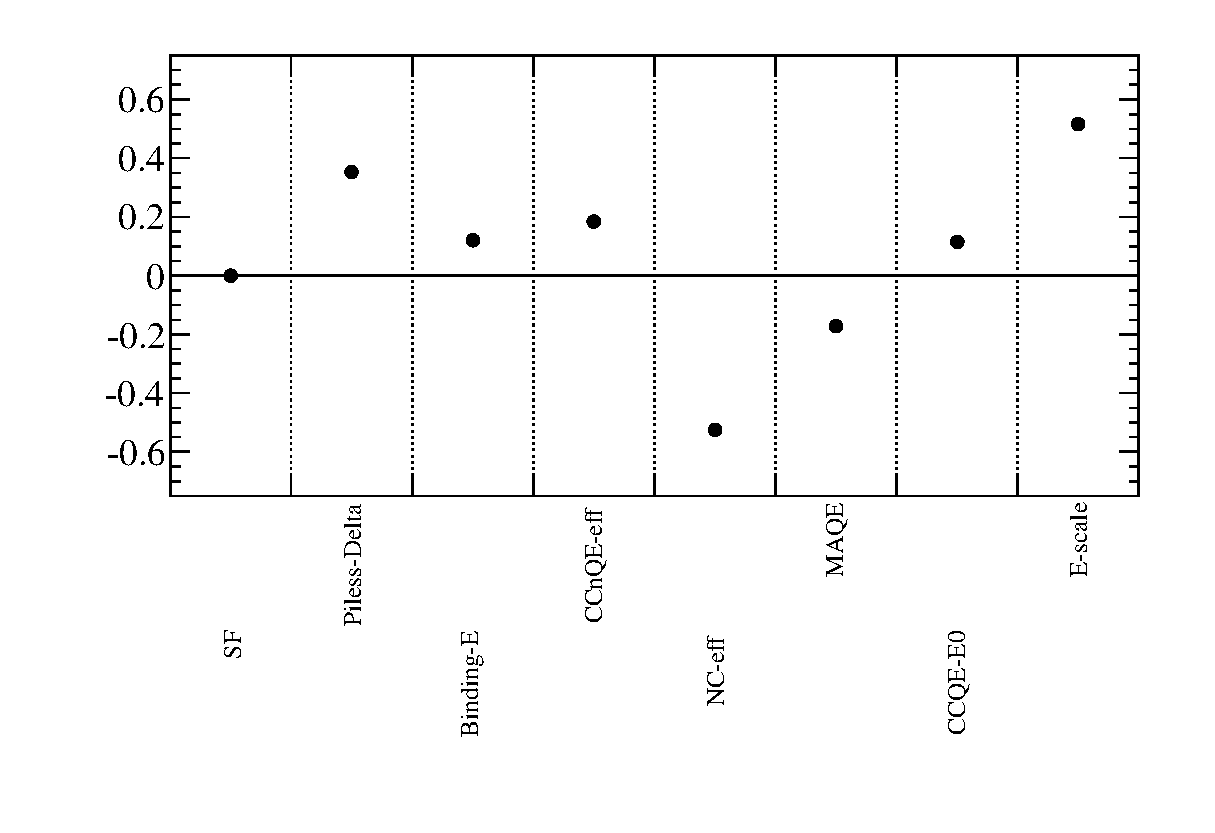
\includegraphics[width=14pc,angle=270]{./images/fit_toymc/example_fits/pulls_0}
\caption {
  Systematic pulls for the 2+8 fit to fake data set 0.
}
\label{fig:fakedata_pulls_0}
\end{minipage}
\hspace{0.06\linewidth}
\begin{minipage}[t]{0.48\linewidth}
\center
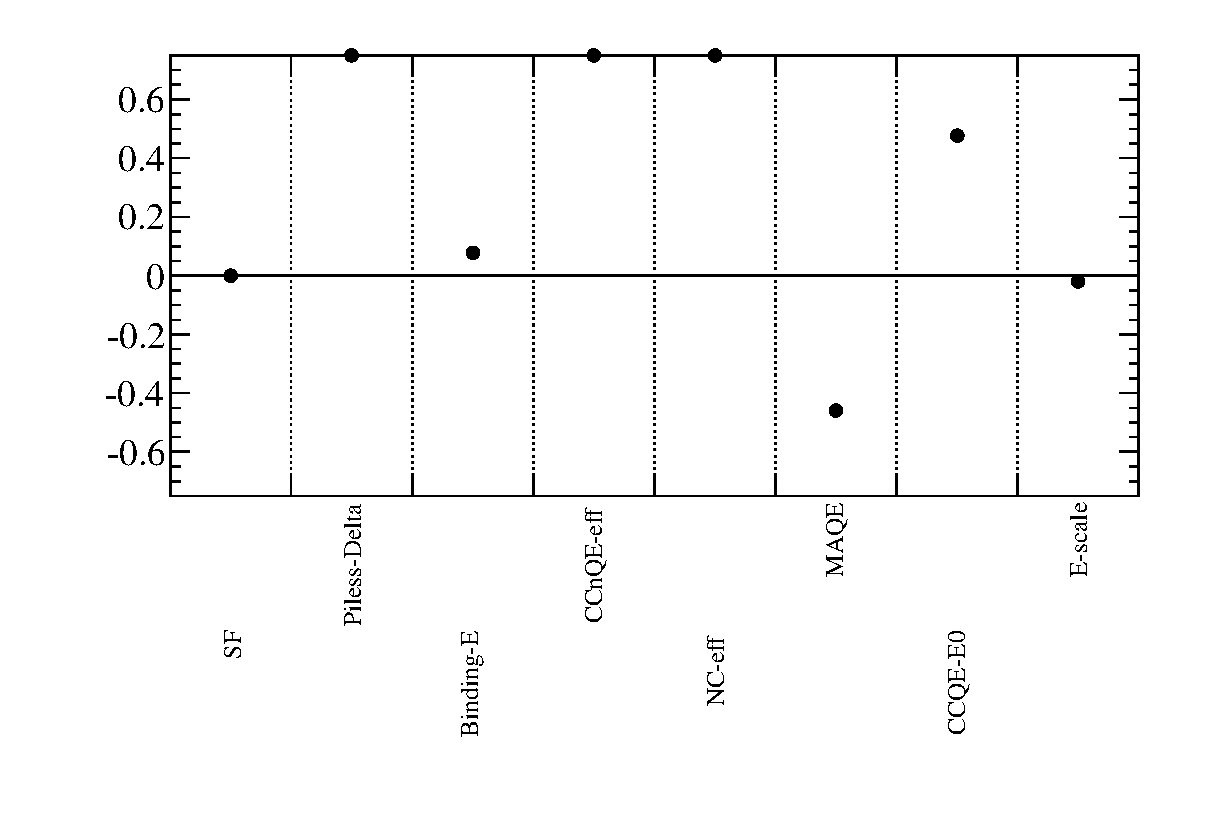
\includegraphics[width=14pc,angle=270]{./images/fit_toymc/example_fits/pulls_1}
\caption { 
  Systematic pulls for the 2+8 fit to fake data set 1.
}
\label{fig:fakedata_pulls_1}
\end{minipage}
\vfill
\begin{minipage}[t]{0.48\linewidth}
\center
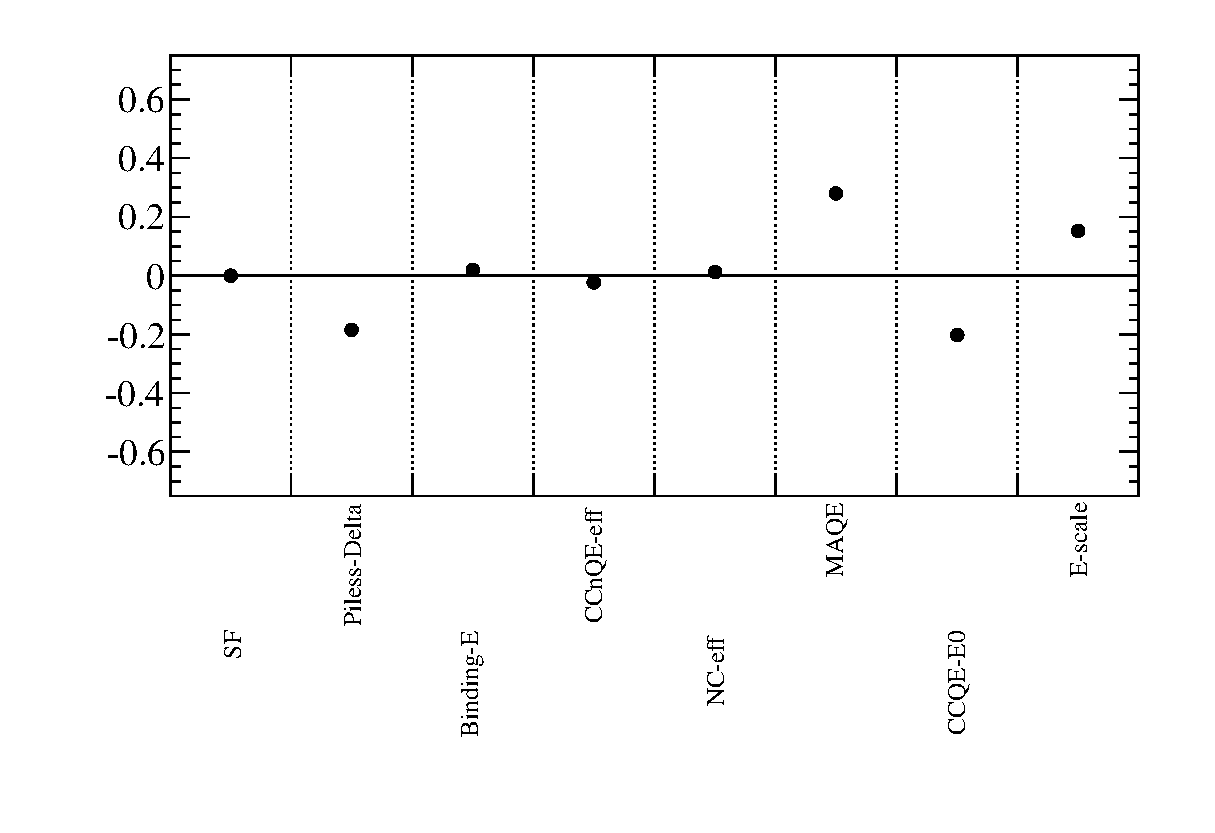
\includegraphics[width=14pc,angle=270]{./images/fit_toymc/example_fits/pulls_2}
\caption {
  Systematic pulls for the 2+8 fit to fake data set 2.
}
\label{fig:fakedata_pulls_2}
\end{minipage}
\hspace{0.06\linewidth}
\begin{minipage}[t]{0.48\linewidth}
\center
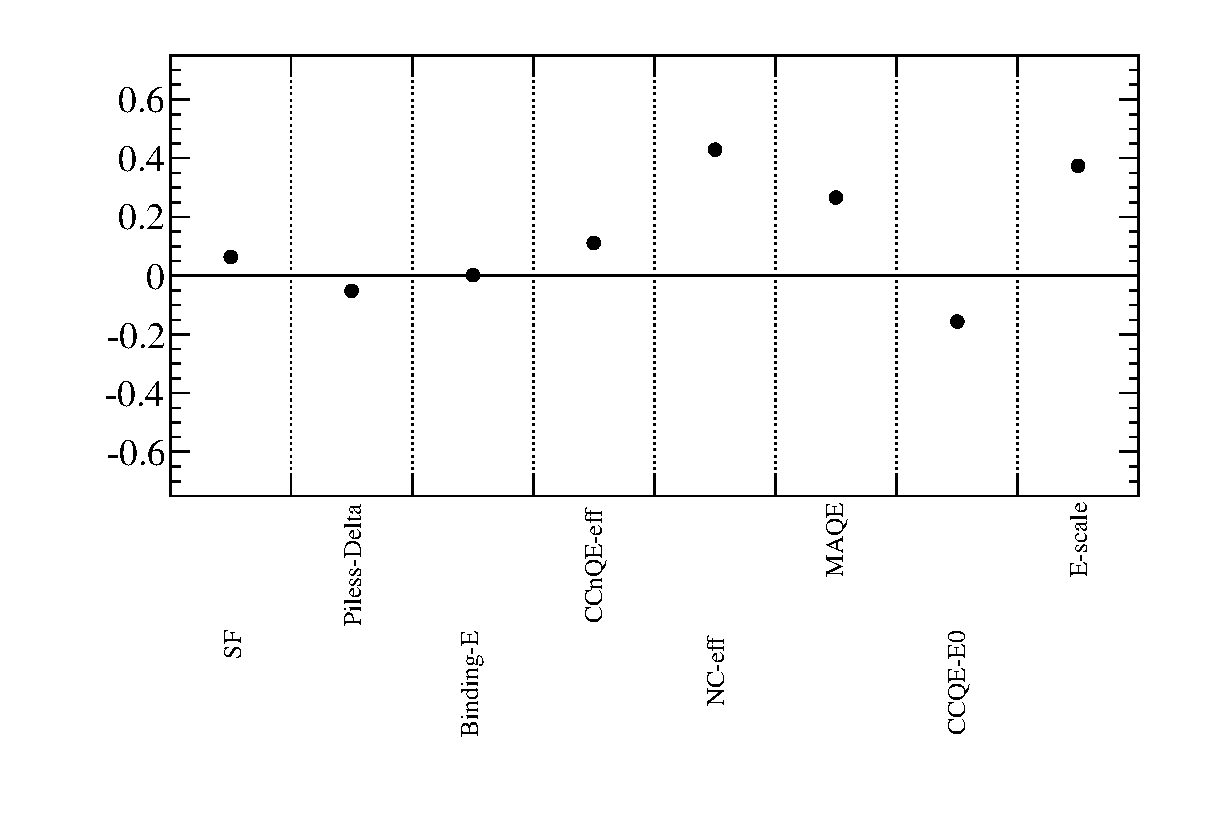
\includegraphics[width=14pc,angle=270]{./images/fit_toymc/example_fits/pulls_3}
\caption { 
  Systematic pulls for the 2+8 fit to fake data set 3.
}
\label{fig:fakedata_pulls_3}
\end{minipage}
\vfill
\begin{minipage}[t]{0.48\linewidth}
\center
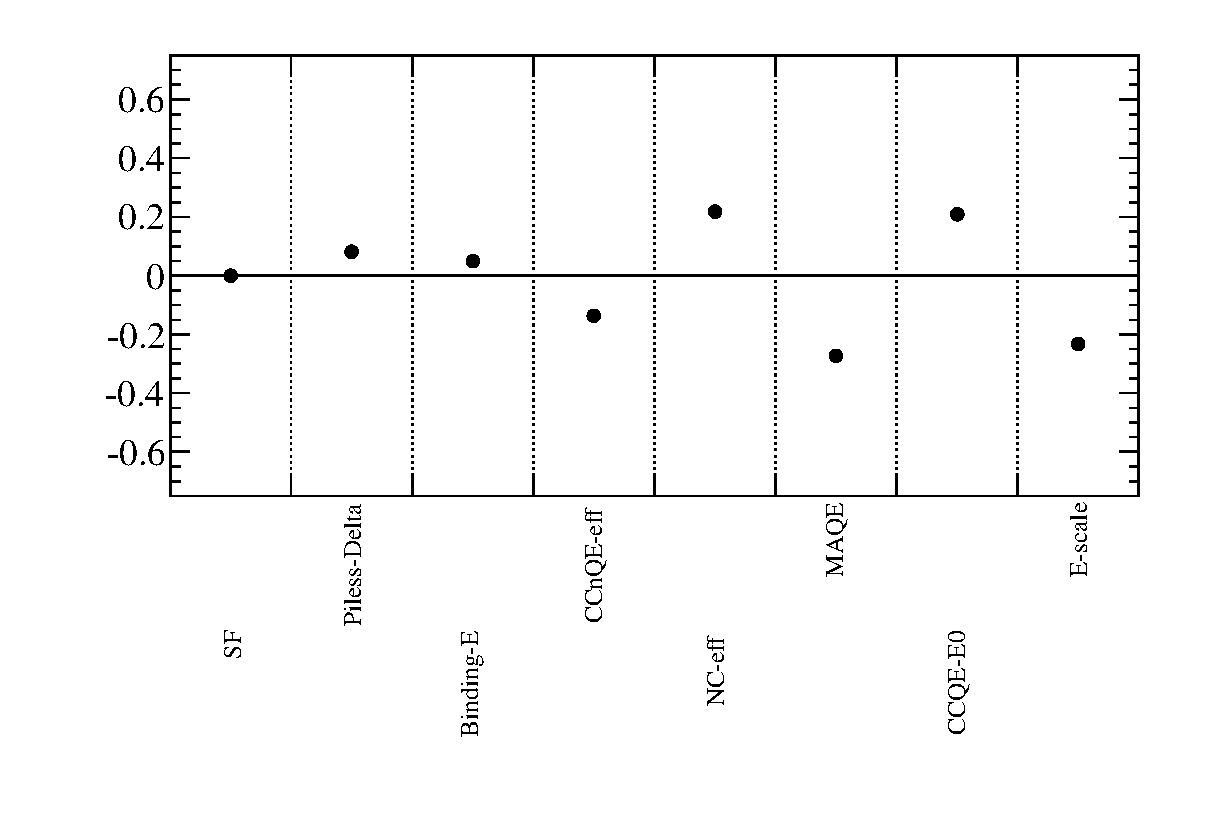
\includegraphics[width=14pc,angle=270]{./images/fit_toymc/example_fits/pulls_4}
\caption {
  Systematic pulls for the 2+8 fit to fake data set 4.
}
\label{fig:fakedata_pulls_4}
\end{minipage}
\hspace{0.06\linewidth}
\begin{minipage}[t]{0.48\linewidth}
\center
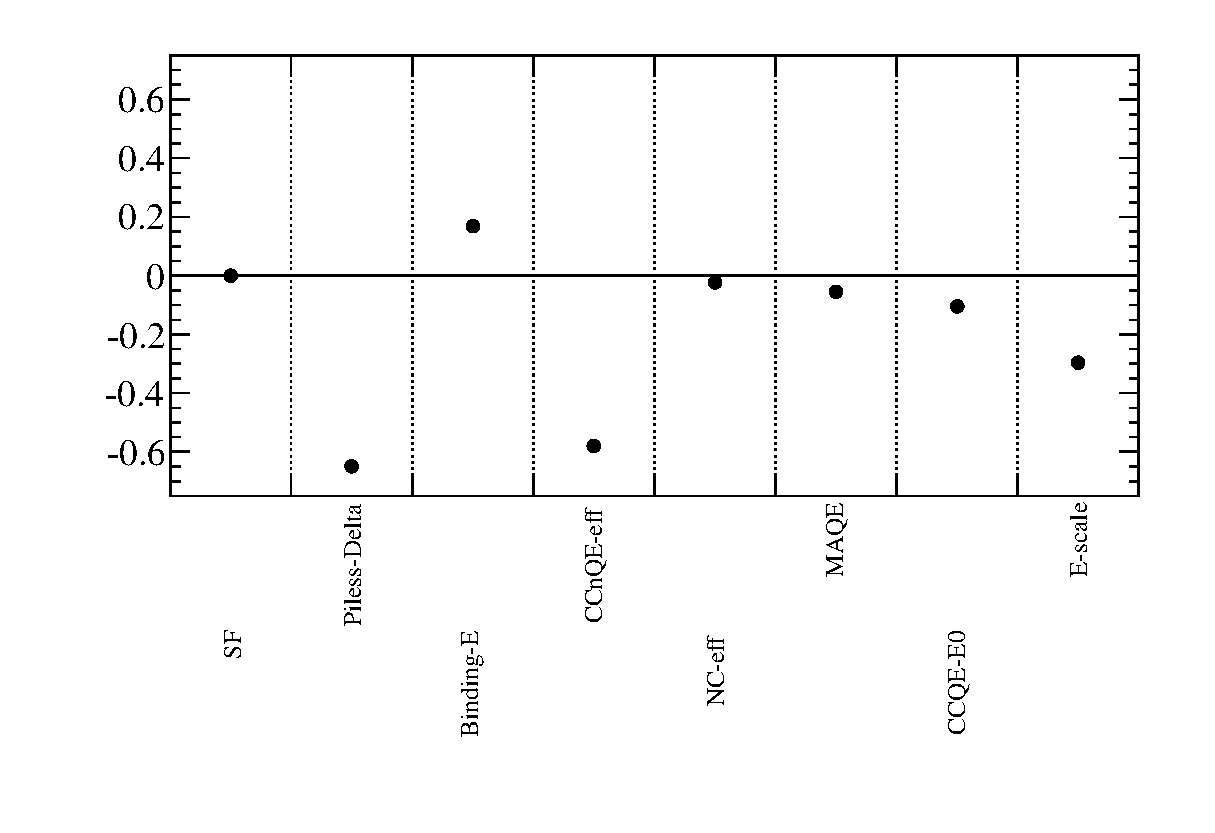
\includegraphics[width=14pc,angle=270]{./images/fit_toymc/example_fits/pulls_5}
\caption { 
  Systematic pulls for the 2+8 fit to fake data set 5.
}
\label{fig:fakedata_pulls_5}
\end{minipage}
\end{figure*}


%...........................................................
%
% Systematic parameter pulls for `2+N' fits
%

\begin{figure*}[htb]
\begin{minipage}[t]{0.48\linewidth}
\center
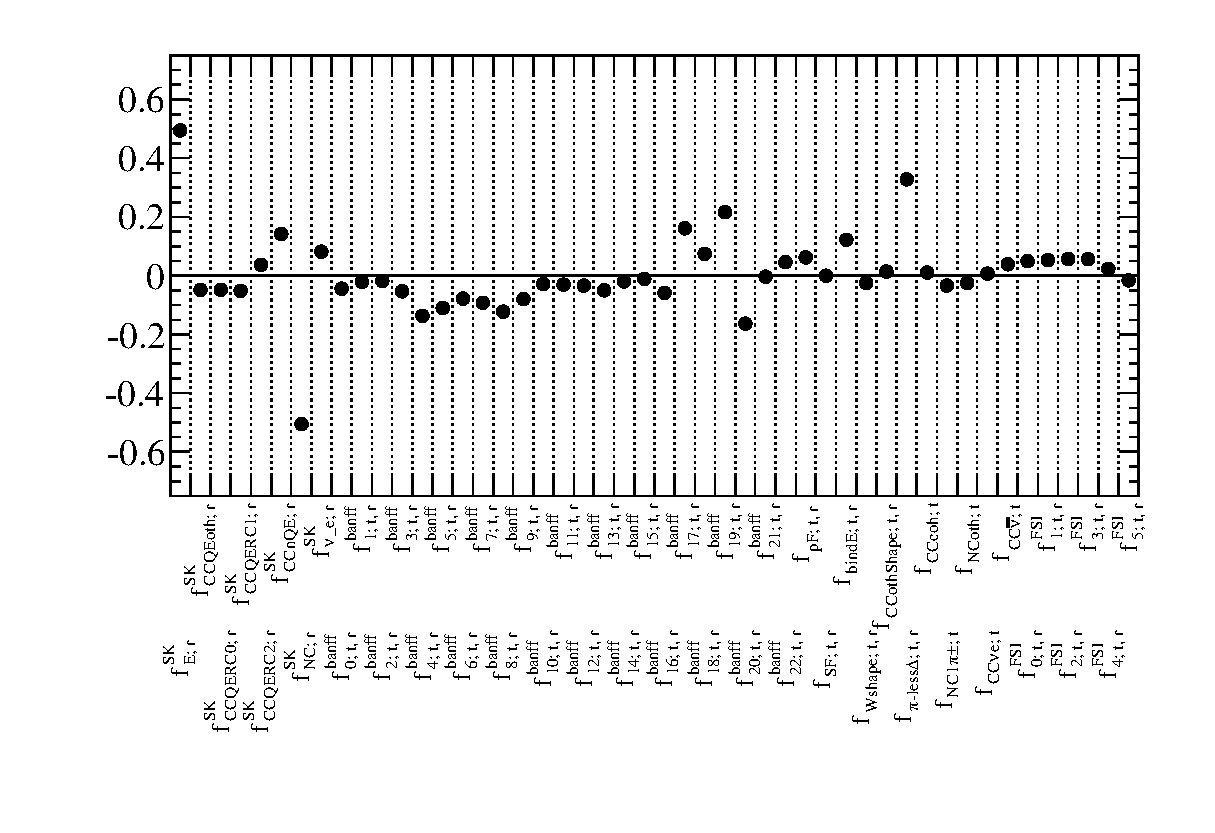
\includegraphics[width=18pc,angle=270]{./images/fit_toymc/example_fits/2N/pulls_0}
\caption {
  Systematic pulls for the 2+N fit to fake data set 0.
}
\label{fig:fakedata_pulls_2N_0}
\end{minipage}
\hspace{0.06\linewidth}
\begin{minipage}[t]{0.48\linewidth}
\center
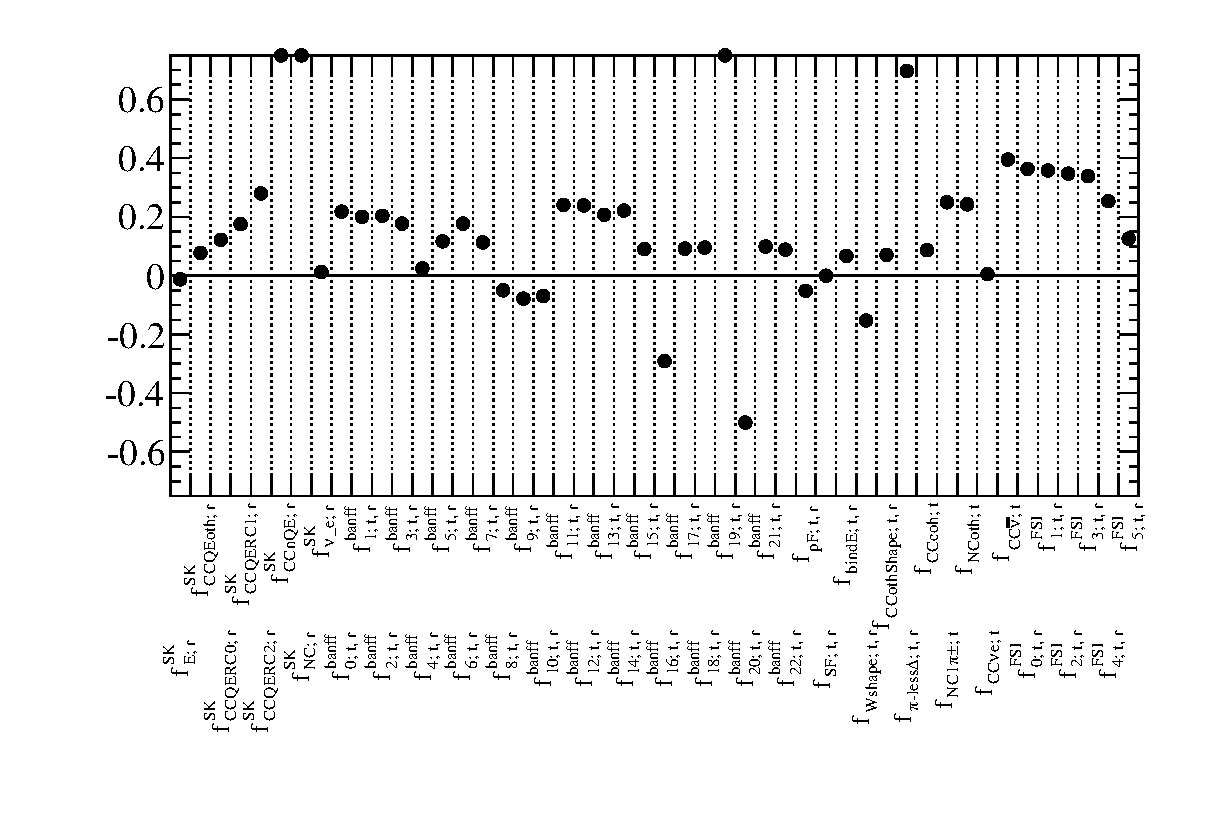
\includegraphics[width=18pc,angle=270]{./images/fit_toymc/example_fits/2N/pulls_1}
\caption { 
  Systematic pulls for the 2+N fit to fake data set 1.
}
\label{fig:fakedata_pulls_2N_1}
\end{minipage}
\vfill
\begin{minipage}[t]{0.48\linewidth}
\center
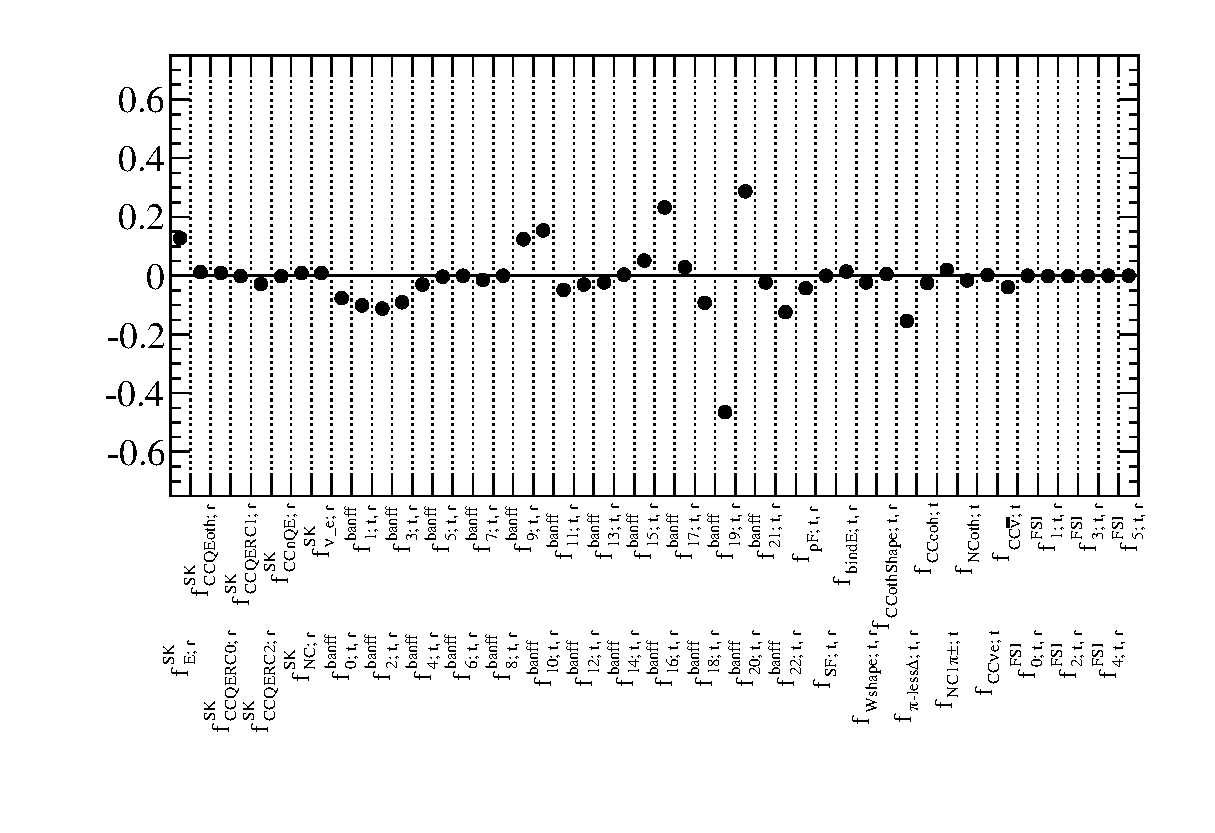
\includegraphics[width=18pc,angle=270]{./images/fit_toymc/example_fits/2N/pulls_2}
\caption {
  Systematic pulls for the 2+N fit to fake data set 2.
}
\label{fig:fakedata_pulls_2N_2}
\end{minipage}
\hspace{0.06\linewidth}
\begin{minipage}[t]{0.48\linewidth}
\center
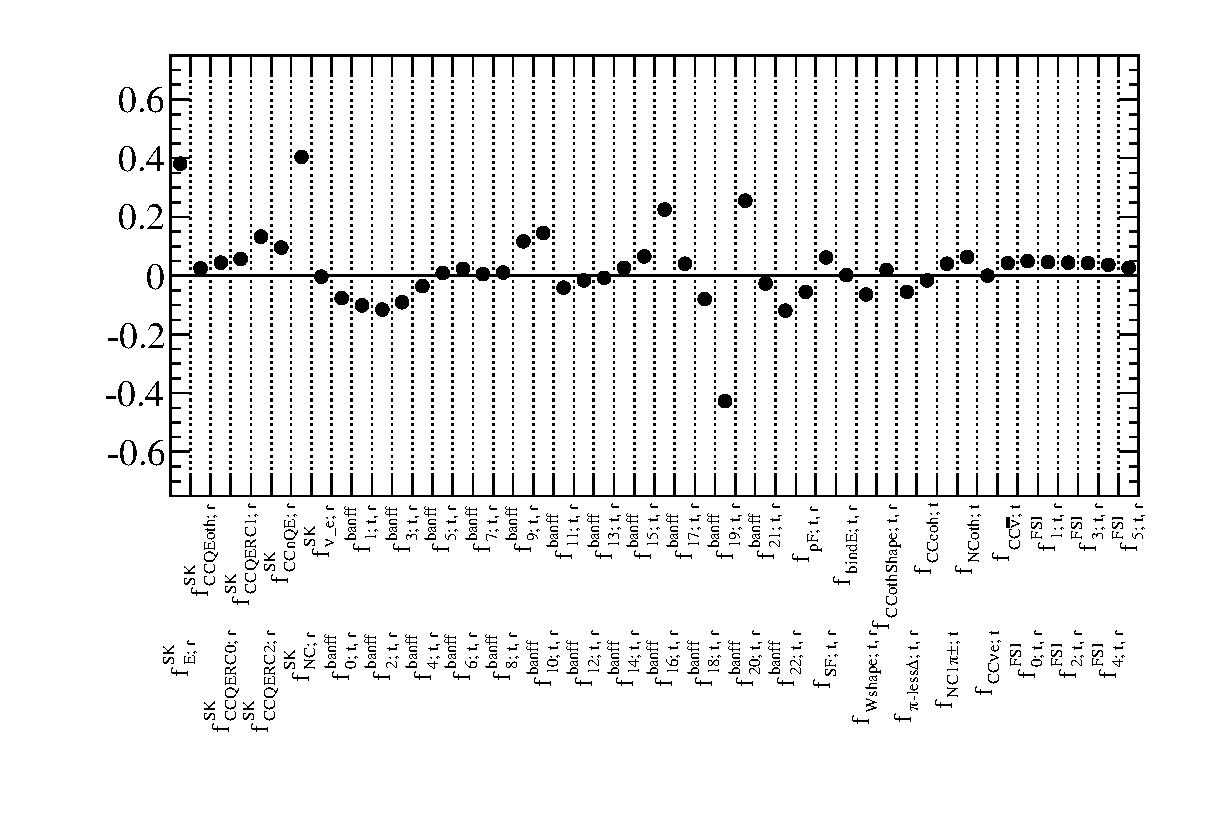
\includegraphics[width=18pc,angle=270]{./images/fit_toymc/example_fits/2N/pulls_3}
\caption { 
  Systematic pulls for the 2+N fit to fake data set 3.
}
\label{fig:fakedata_pulls_2N_3}
\end{minipage}
\vfill
\begin{minipage}[t]{0.48\linewidth}
\center
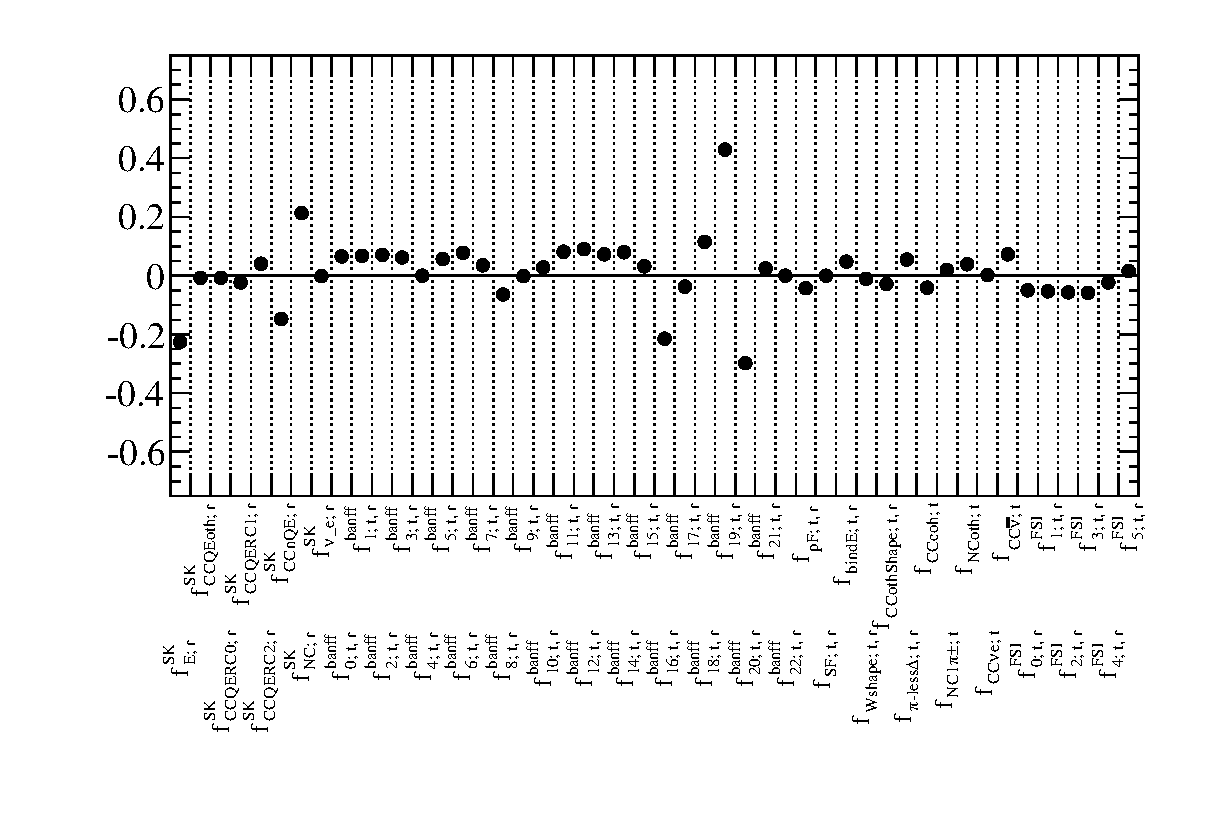
\includegraphics[width=18pc,angle=270]{./images/fit_toymc/example_fits/2N/pulls_4}
\caption {
  Systematic pulls for the 2+N fit to fake data set 4.
}
\label{fig:fakedata_pulls_2N_4}
\end{minipage}
\hspace{0.06\linewidth}
\begin{minipage}[t]{0.48\linewidth}
\center
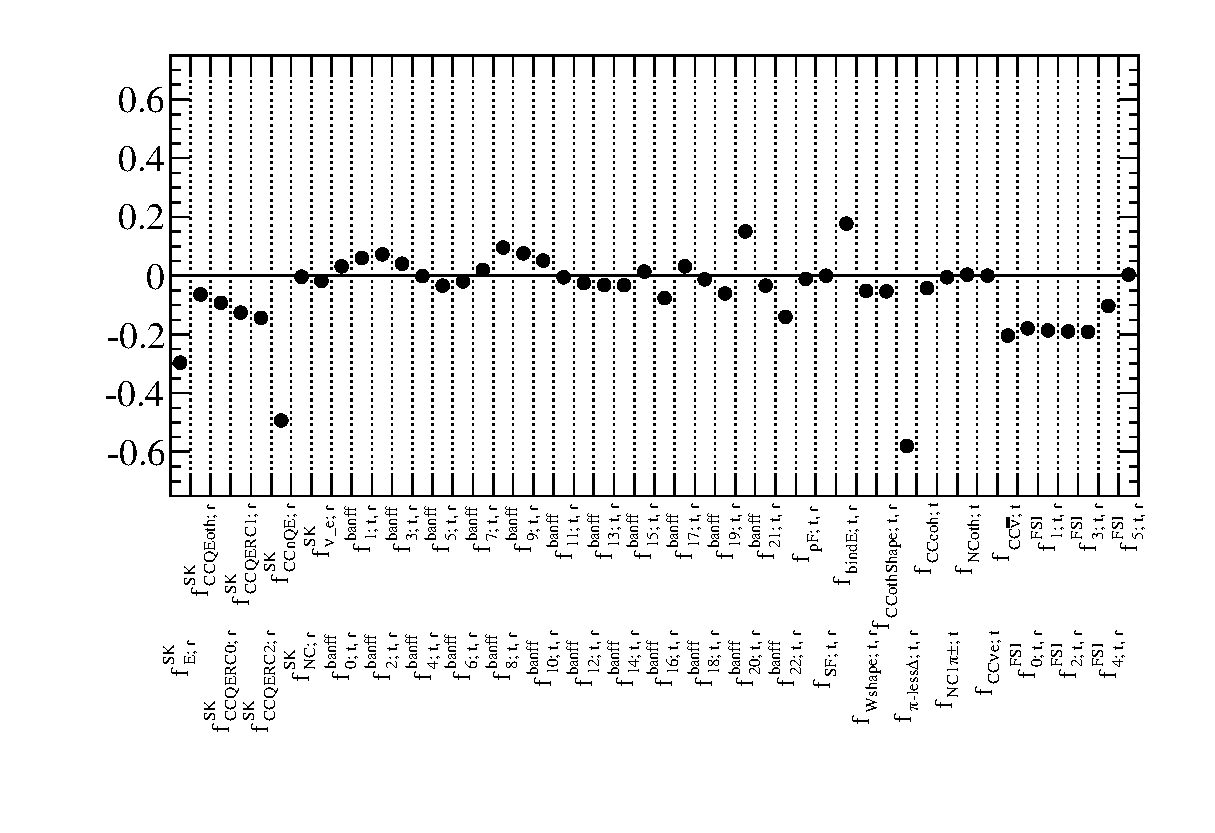
\includegraphics[width=18pc,angle=270]{./images/fit_toymc/example_fits/2N/pulls_5}
\caption { 
  Systematic pulls for the 2+N fit to fake data set 5.
}
\label{fig:fakedata_pulls_2N_5}
\end{minipage}
\end{figure*}

\clearpage

\subsection{Goodness of fit}
\label{appendix:example_toy_mc_fits:goodness}

%...........................................................
%
% Goodness of fit for `2+N' fits
%

% \begin{figure*}[htb]
% \begin{minipage}[t]{0.48\linewidth}
% \center
% \includegraphics[width=18pc]{./images/fit_toymc/example_fits/2N/goodness_0}
% \caption {
%   Distribution of $\chi^2_{gof}$ from 1000 toy MC at the best fit oscillation point for the 2+N fit to fake data set 0.
%   The $\chi^2_{gof}$ for data is highlighted.
% }
% \label{fig:fakedata_goodness_2N_0}
% \end{minipage}
% \hspace{0.06\linewidth}
% \begin{minipage}[t]{0.48\linewidth}
% \center
% \includegraphics[width=18pc]{./images/fit_toymc/example_fits/2N/goodness_1}
% \caption { 
%   Distribution of $\chi^2_{gof}$ from 1000 toy MC at the best fit oscillation point for the 2+N fit to fake data set 1.
%   The $\chi^2_{gof}$ for data is highlighted.
% }
% \label{fig:fakedata_goodness_2N_1}
% \end{minipage}
% \vfill
% \begin{minipage}[t]{0.48\linewidth}
% \center
% \includegraphics[width=18pc]{./images/fit_toymc/example_fits/2N/goodness_2}
% \caption {
%   Distribution of $\chi^2_{gof}$ from 1000 toy MC at the best fit oscillation point for the 2+N fit to fake data set 2.
%   The $\chi^2_{gof}$ for data is highlighted.
% }
% \label{fig:fakedata_goodness_2N_2}
% \end{minipage}
% \hspace{0.06\linewidth}
% \begin{minipage}[t]{0.48\linewidth}
% \center
% \includegraphics[width=18pc]{./images/fit_toymc/example_fits/2N/goodness_3}
% \caption { 
%   Distribution of $\chi^2_{gof}$ from 1000 toy MC at the best fit oscillation point for the 2+N fit to fake data set 3.
%   The $\chi^2_{gof}$ for data is highlighted.
% }
% \label{fig:fakedata_goodness_2N_3}
% \end{minipage}
% \vfill
% \begin{minipage}[t]{0.48\linewidth}
% \center
% \includegraphics[width=18pc]{./images/fit_toymc/example_fits/2N/goodness_4}
% \caption {
%   Distribution of $\chi^2_{gof}$ from 1000 toy MC at the best fit oscillation point for the 2+N fit to fake data set 4.
%   The $\chi^2_{gof}$ for data is highlighted.
% }
% \label{fig:fakedata_goodness_2N_4}
% \end{minipage}
% \hspace{0.06\linewidth}
% \begin{minipage}[t]{0.48\linewidth}
% \center
% \includegraphics[width=18pc]{./images/fit_toymc/example_fits/2N/goodness_5}
% \caption { 
%   Distribution of $\chi^2_{gof}$ from 1000 toy MC at the best fit oscillation point for the 2+N fit to fake data set 5.
%   The $\chi^2_{gof}$ for data is highlighted.
% }
% \label{fig:fakedata_goodness_2N_5}
% \end{minipage}
% \end{figure*}

%...........................................................
%
% Goodness of fit for `2+8' fits
%

\begin{figure*}[htb]
\begin{minipage}[t]{0.48\linewidth}
\center
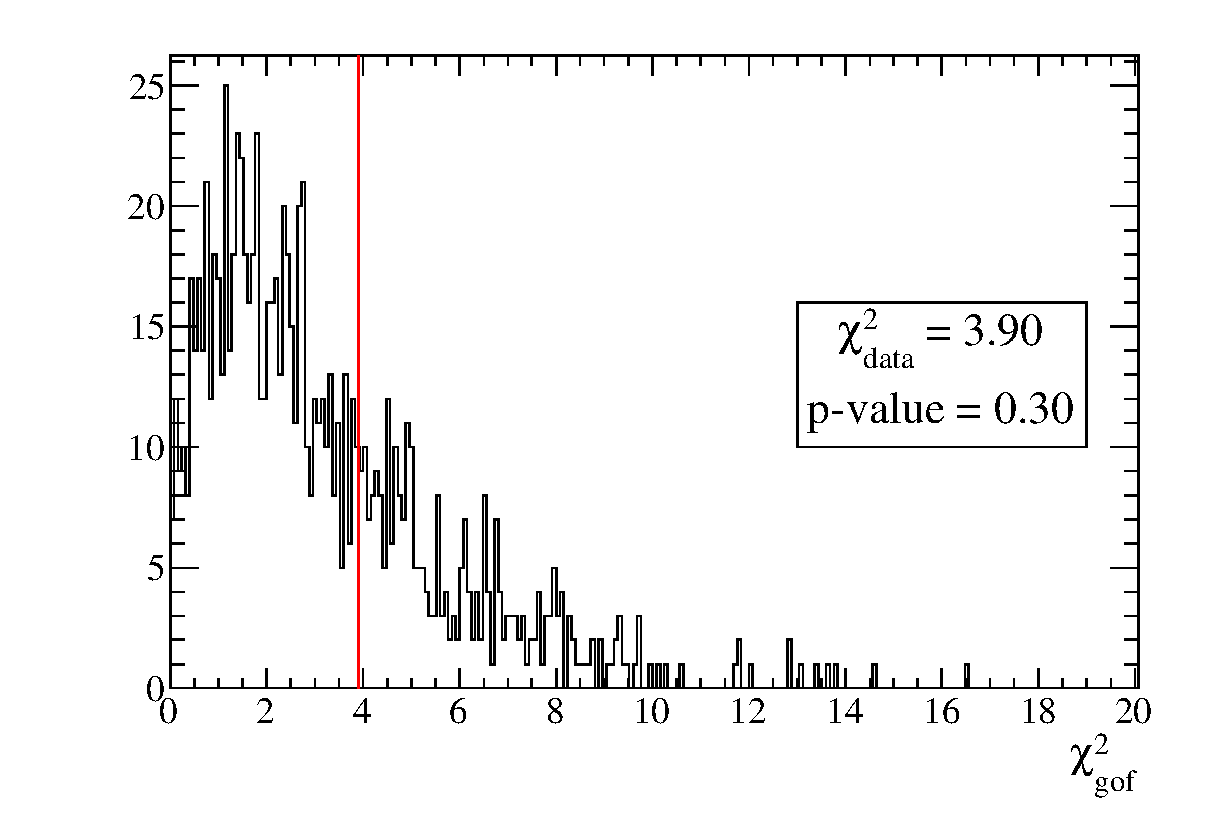
\includegraphics[width=18pc]{./images/fit_toymc/example_fits/goodness_0}
\caption {
  Distribution of $\chi^2_{gof}$ from 1000 toy MC datasets at the best-fit oscillation point for the 2+8 fit to fake data set 0.
  The $\chi^2_{gof}$ for data is highlighted.
}
\label{fig:fakedata_goodness_0}
\end{minipage}
\hspace{0.06\linewidth}
\begin{minipage}[t]{0.48\linewidth}
\center
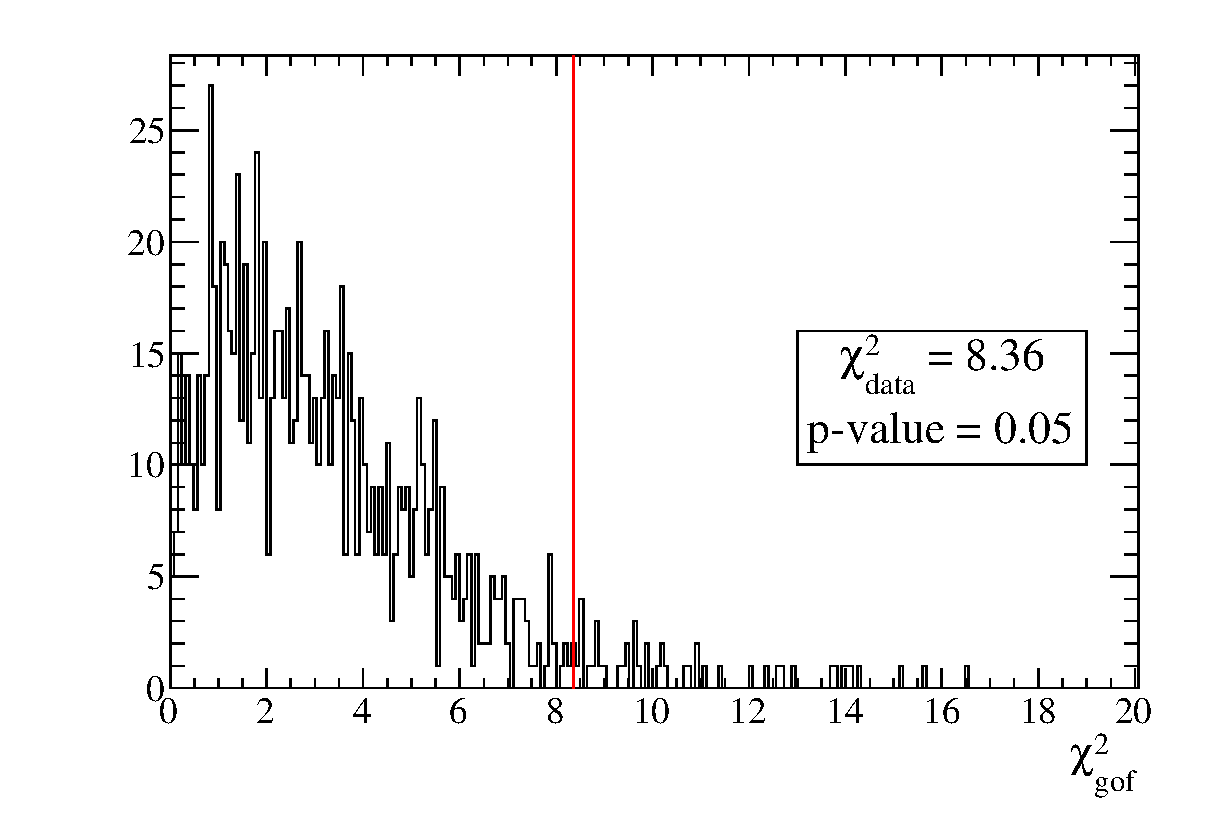
\includegraphics[width=18pc]{./images/fit_toymc/example_fits/goodness_1}
\caption { 
  Distribution of $\chi^2_{gof}$ from 1000 toy MC datasets at the best-fit oscillation point for the 2+8 fit to fake data set 1.
  The $\chi^2_{gof}$ for data is highlighted.
}
\label{fig:fakedata_goodness_1}
\end{minipage}
\vfill
\begin{minipage}[t]{0.48\linewidth}
\center
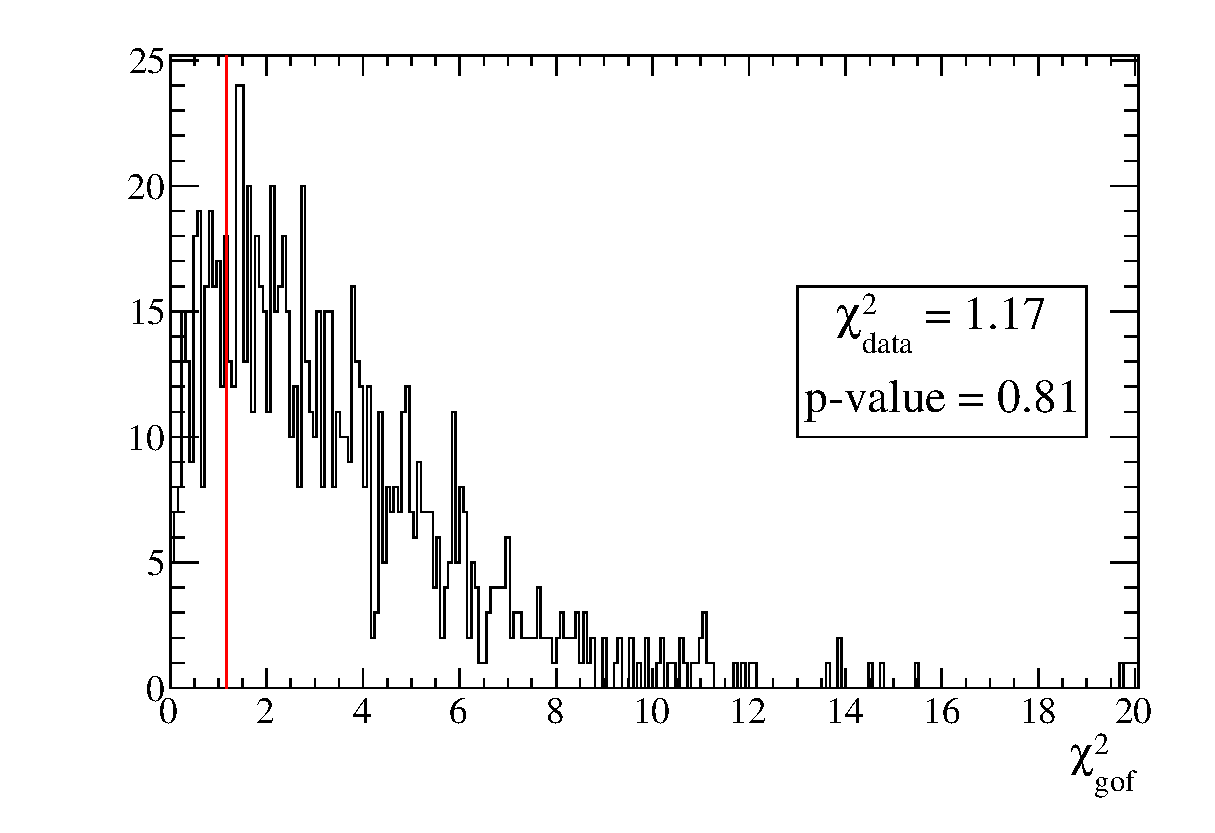
\includegraphics[width=18pc]{./images/fit_toymc/example_fits/goodness_2}
\caption {
  Distribution of $\chi^2_{gof}$ from 1000 toy MC datasets at the best-fit oscillation point for the 2+8 fit to fake data set 2.
  The $\chi^2_{gof}$ for data is highlighted.
}
\label{fig:fakedata_goodness_2}
\end{minipage}
\hspace{0.06\linewidth}
\begin{minipage}[t]{0.48\linewidth}
\center
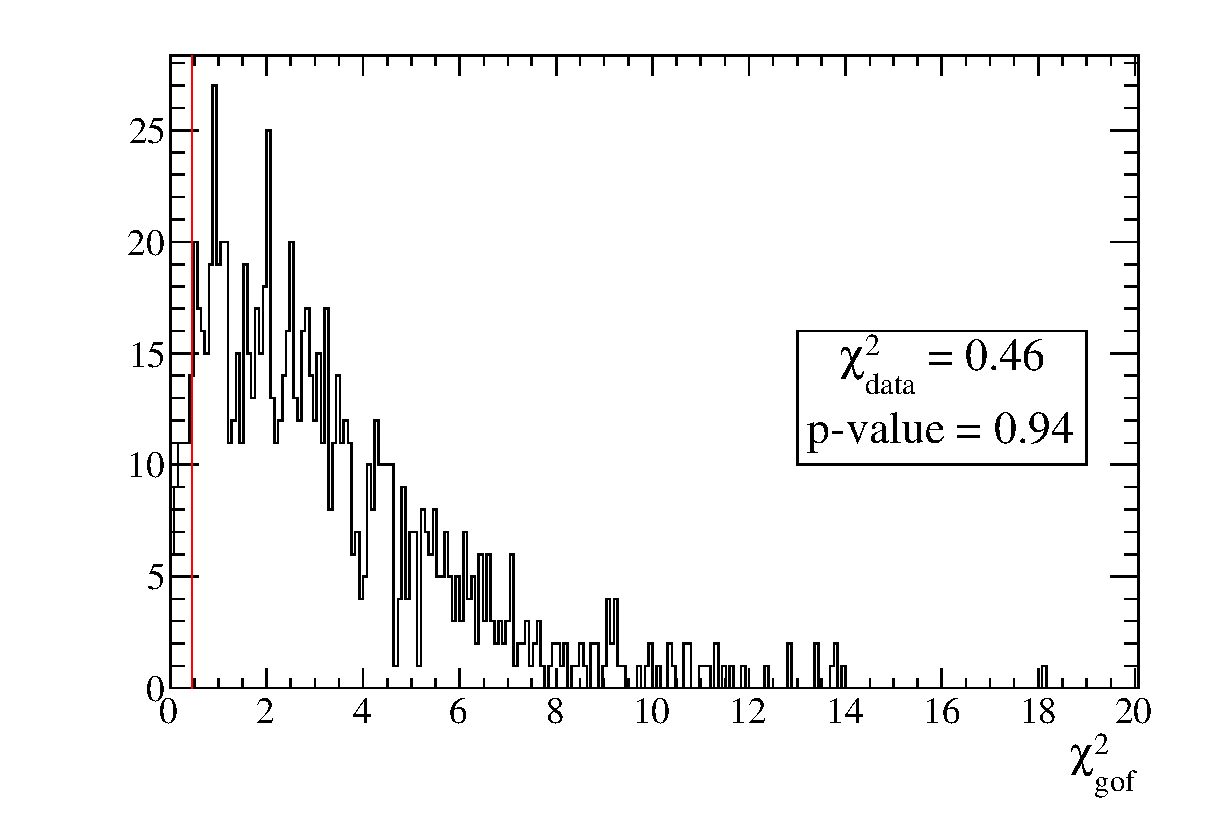
\includegraphics[width=18pc]{./images/fit_toymc/example_fits/goodness_3}
\caption { 
  Distribution of $\chi^2_{gof}$ from 1000 toy MC datasets at the best-fit oscillation point for the 2+8 fit to fake data set 3.
  The $\chi^2_{gof}$ for data is highlighted.
}
\label{fig:fakedata_goodness_3}
\end{minipage}
\vfill
\begin{minipage}[t]{0.48\linewidth}
\center
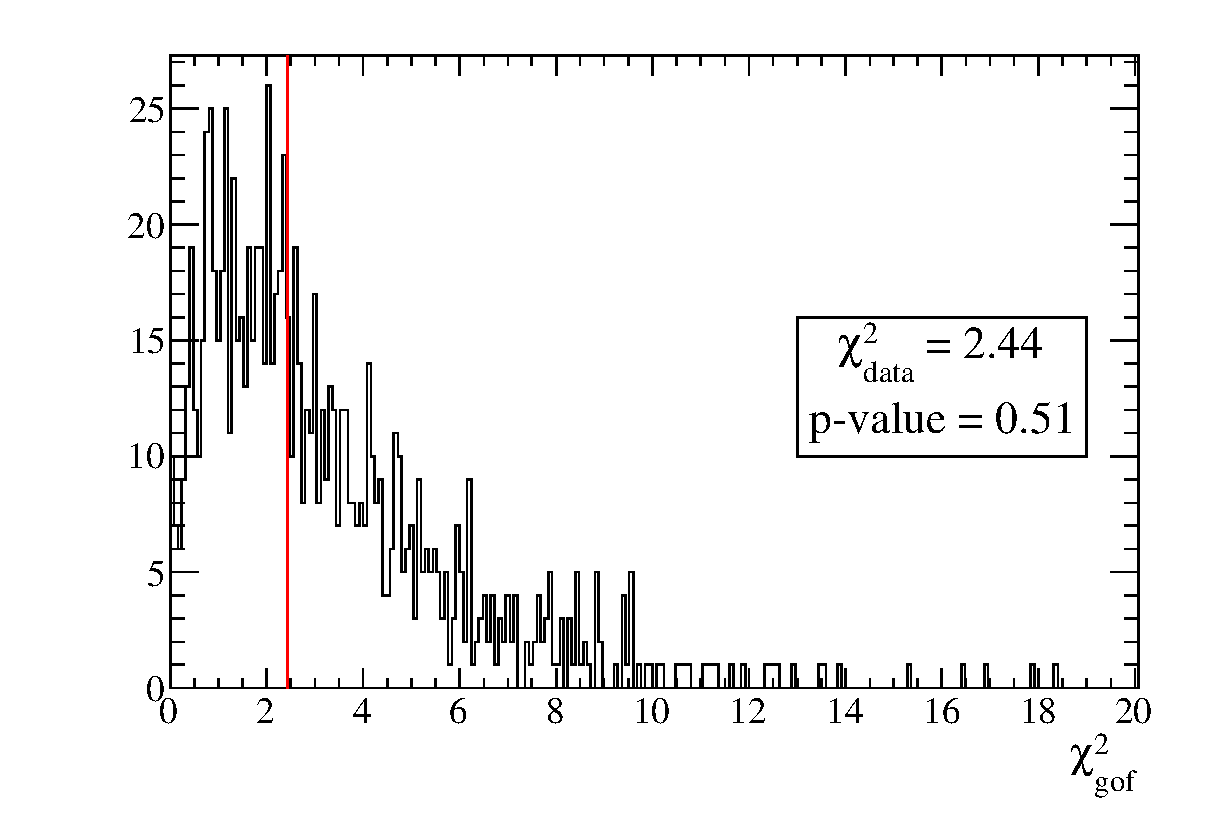
\includegraphics[width=18pc]{./images/fit_toymc/example_fits/goodness_4}
\caption {
  Distribution of $\chi^2_{gof}$ from 1000 toy MC datasets at the best-fit oscillation point for the 2+8 fit to fake data set 4.
  The $\chi^2_{gof}$ for data is highlighted.
}
\label{fig:fakedata_goodness_4}
\end{minipage}
\hspace{0.06\linewidth}
\begin{minipage}[t]{0.48\linewidth}
\center
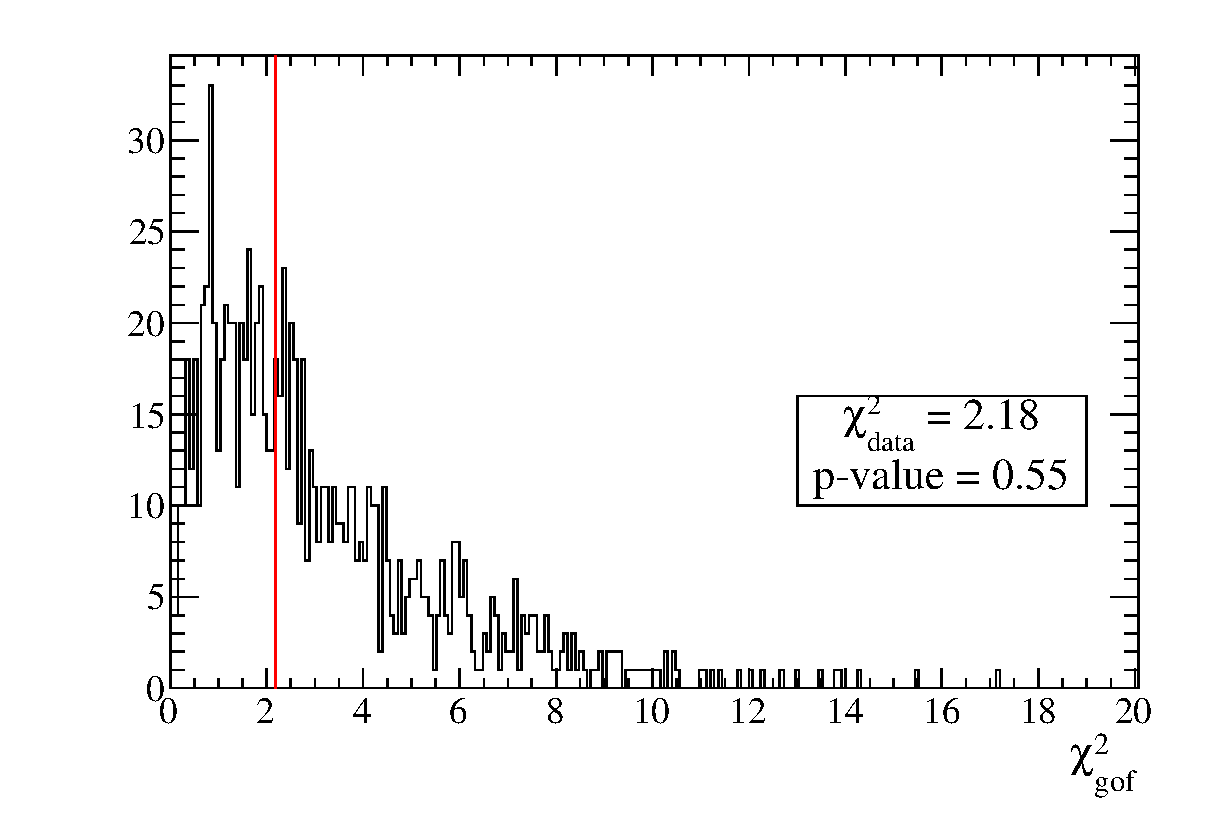
\includegraphics[width=18pc]{./images/fit_toymc/example_fits/goodness_5}
\caption { 
  Distribution of $\chi^2_{gof}$ from 1000 toy MC datasets at the best-fit oscillation point for the 2+8 fit to fake data set 5.
  The $\chi^2_{gof}$ for data is highlighted.
}
\label{fig:fakedata_goodness_5}
\end{minipage}
\end{figure*}


\clearpage
\subsection{Best-fit spectra}
\label{appendix:example_toy_mc_fits:spectra}

%...........................................................
%
% Best-fit spectra and ratios for `2+N' fits
%

\begin{figure*}[htb]
\begin{minipage}[t]{0.48\linewidth}
\center
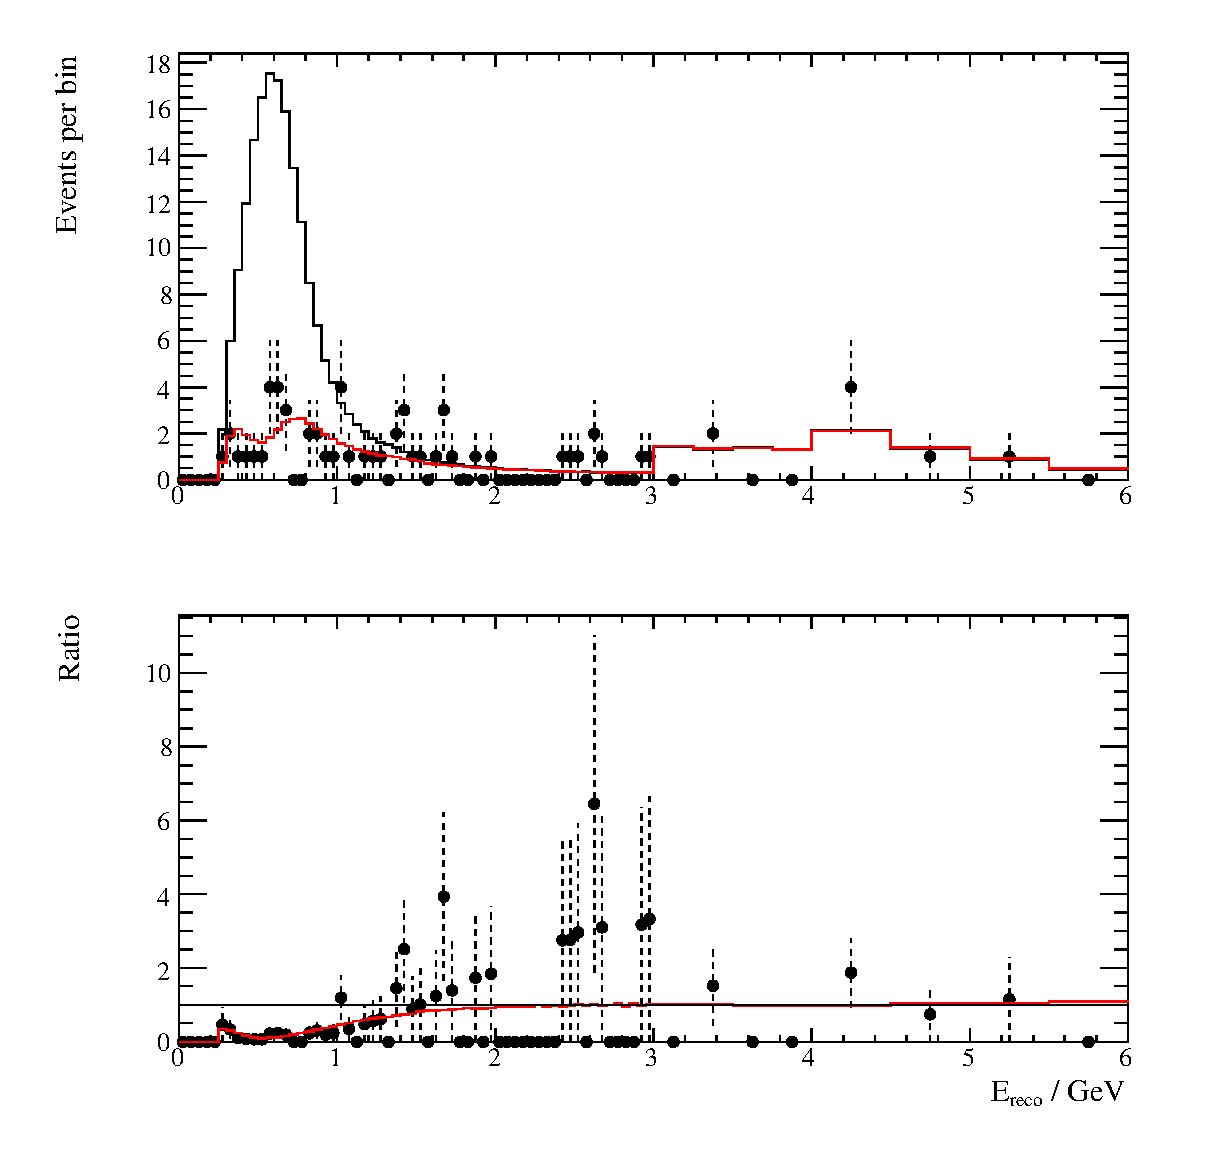
\includegraphics[width=13pc]{./images/fit_toymc/example_fits/2N/spectrum_0}
\caption {
  Best-fit spectrum (top) and ratios of data and best-fit spectrum to predicted spectrum 
  for no oscillations (bottom) for the 2+N fit to fake data set 0
}
\label{fig:fakedata_spectrum_2N_0}
\end{minipage}
\hspace{0.06\linewidth}
\begin{minipage}[t]{0.48\linewidth}
\center
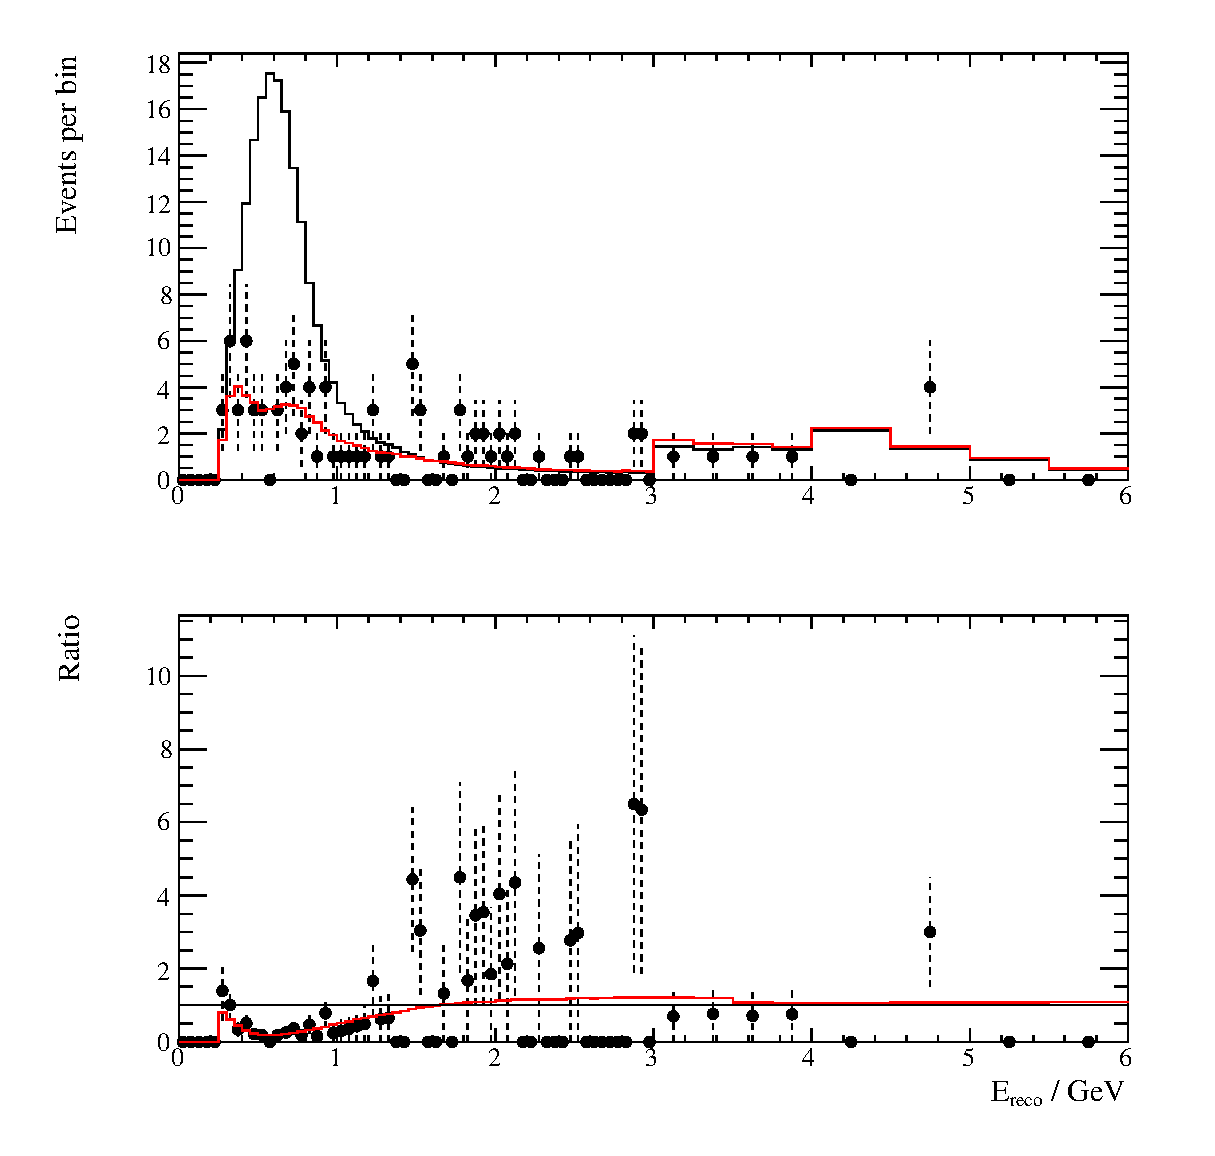
\includegraphics[width=13pc]{./images/fit_toymc/example_fits/2N/spectrum_1}
\caption { 
  Best-fit spectrum (top) and ratios of data and best-fit spectrum to predicted spectrum
  for no oscillations (bottom) for the 2+N fit to fake data set 1
}
\label{fig:fakedata_spectrum_2N_1}
\end{minipage}
\vfill
\begin{minipage}[t]{0.48\linewidth}
\center
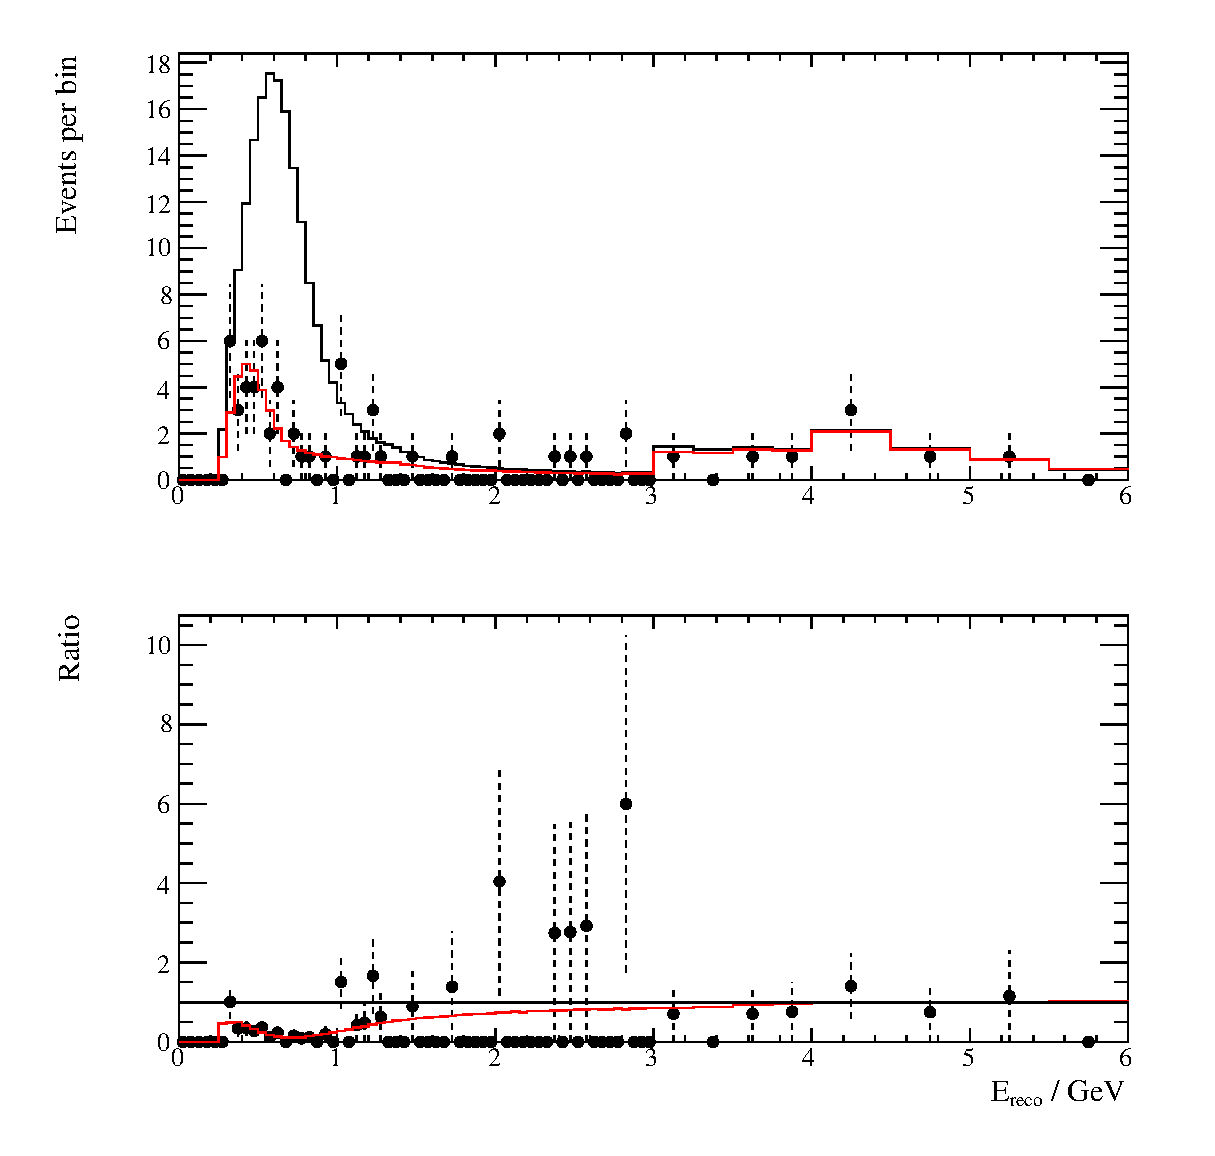
\includegraphics[width=13pc]{./images/fit_toymc/example_fits/2N/spectrum_2}
\caption {
  Best-fit spectrum (top) and ratios of data and best-fit spectrum to predicted spectrum
  for no oscillations (bottom) for the 2+N fit to fake data set 2
}
\label{fig:fakedata_spectrum_2N_2}
\end{minipage}
\hspace{0.06\linewidth}
\begin{minipage}[t]{0.48\linewidth}
\center
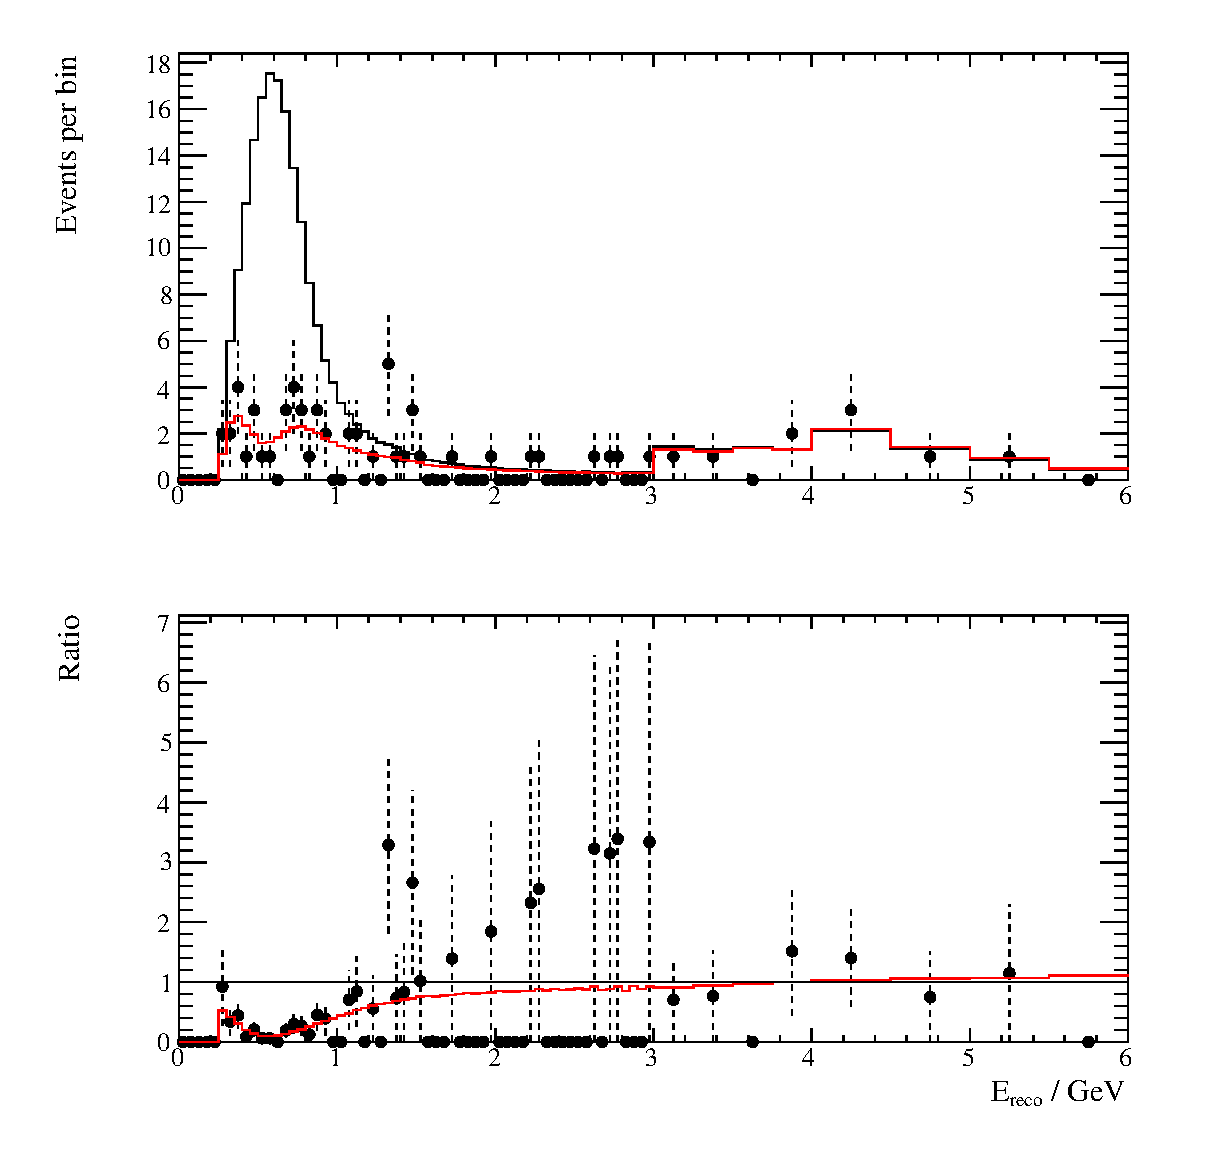
\includegraphics[width=13pc]{./images/fit_toymc/example_fits/2N/spectrum_3}
\caption { 
  Best-fit spectrum (top) and ratios of data and best-fit spectrum to predicted spectrum
  for no oscillations (bottom) for the 2+N fit to fake data set 3
}
\label{fig:fakedata_spectrum_2N_3}
\end{minipage}
\vfill
\begin{minipage}[t]{0.48\linewidth}
\center
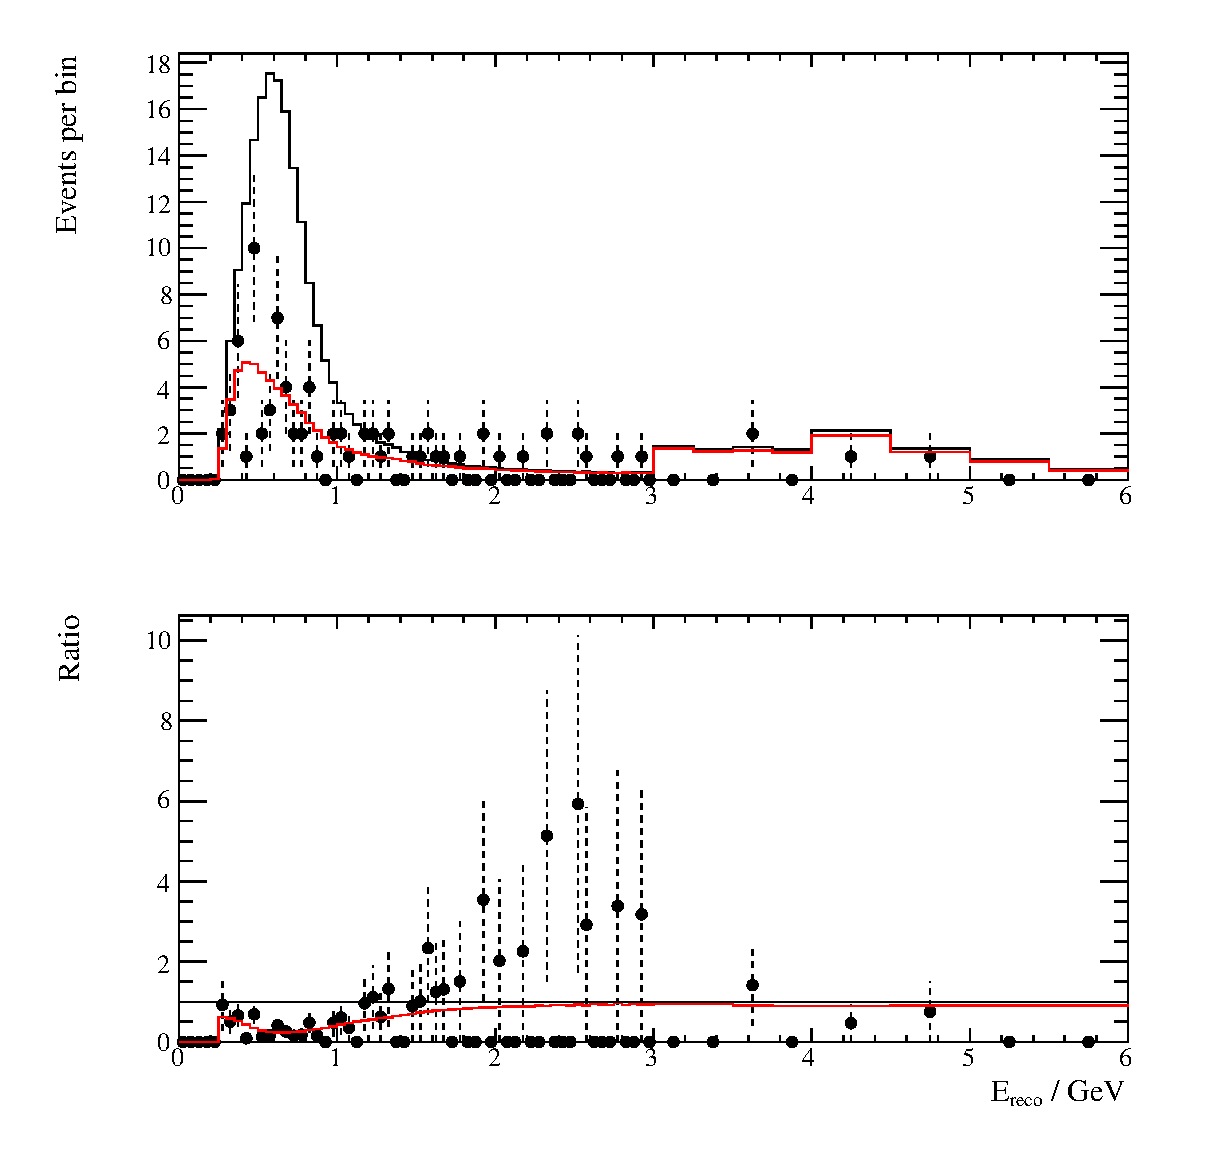
\includegraphics[width=13pc]{./images/fit_toymc/example_fits/2N/spectrum_4}
\caption {
  Best-fit spectrum (top) and ratios of data and best-fit spectrum to predicted spectrum
  for no oscillations (bottom) for the 2+N fit to fake data set 4
}
\label{fig:fakedata_spectrum_2N_4}
\end{minipage}
\hspace{0.06\linewidth}
\begin{minipage}[t]{0.48\linewidth}
\center
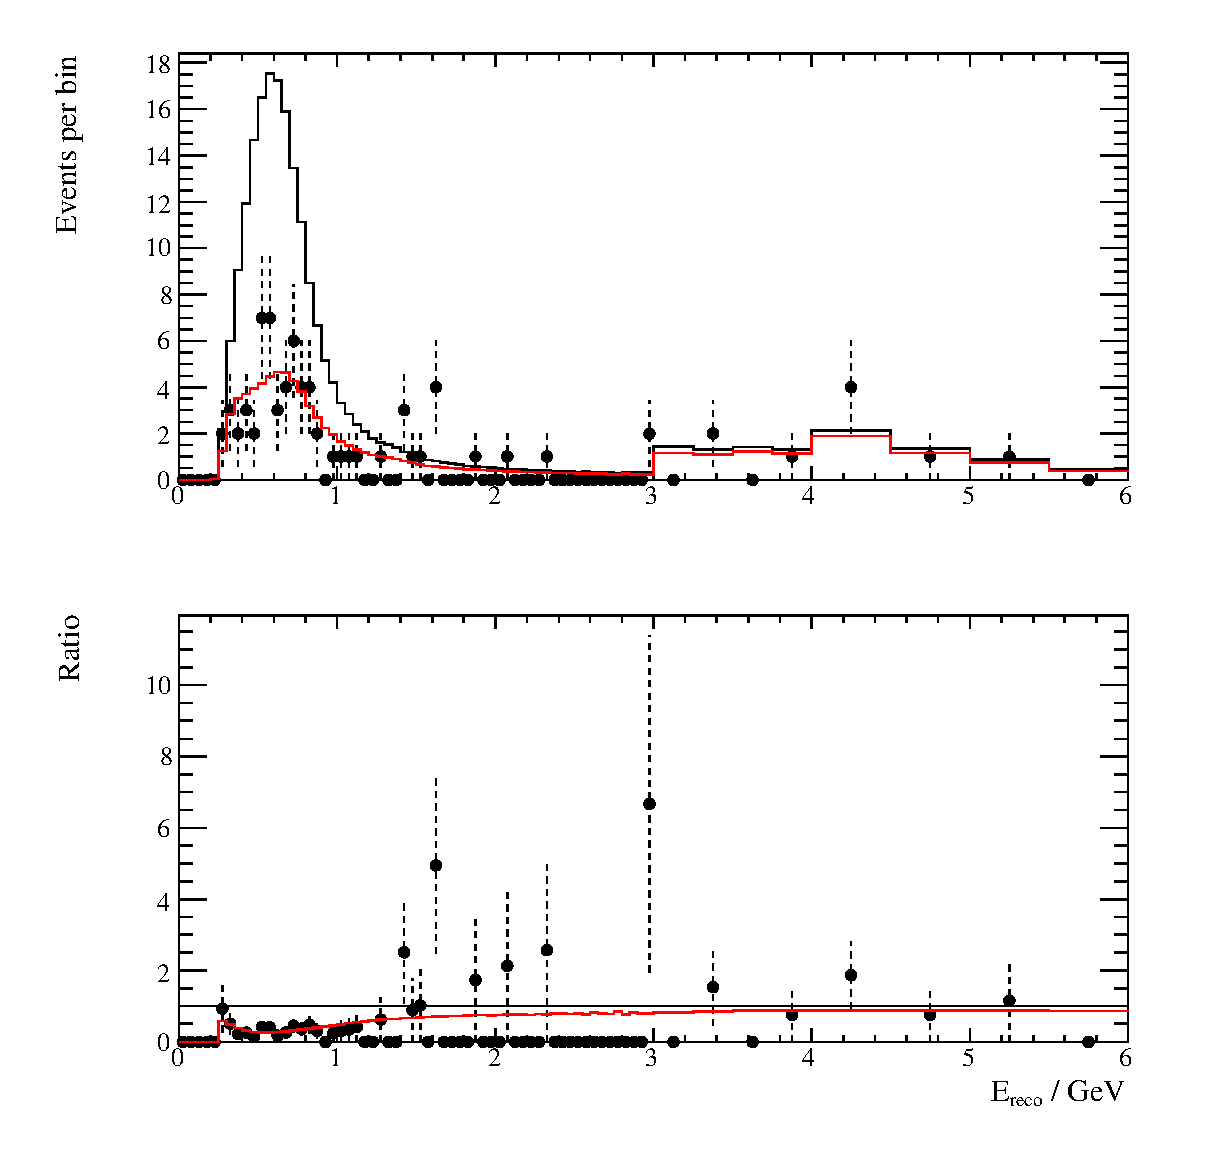
\includegraphics[width=13pc]{./images/fit_toymc/example_fits/2N/spectrum_5}
\caption { 
  Best-fit spectrum (top) and ratios of data and best-fit spectrum to predicted spectrum
  for no oscillations (bottom) for the 2+N fit to fake data set 5
}
\label{fig:fakedata_spectrum_2N_5}
\end{minipage}
\end{figure*}

%...........................................................
%
% Best-fit spectra and ratios for `2+8' fits
%

\begin{figure*}[htb]
\begin{minipage}[t]{0.48\linewidth}
\center
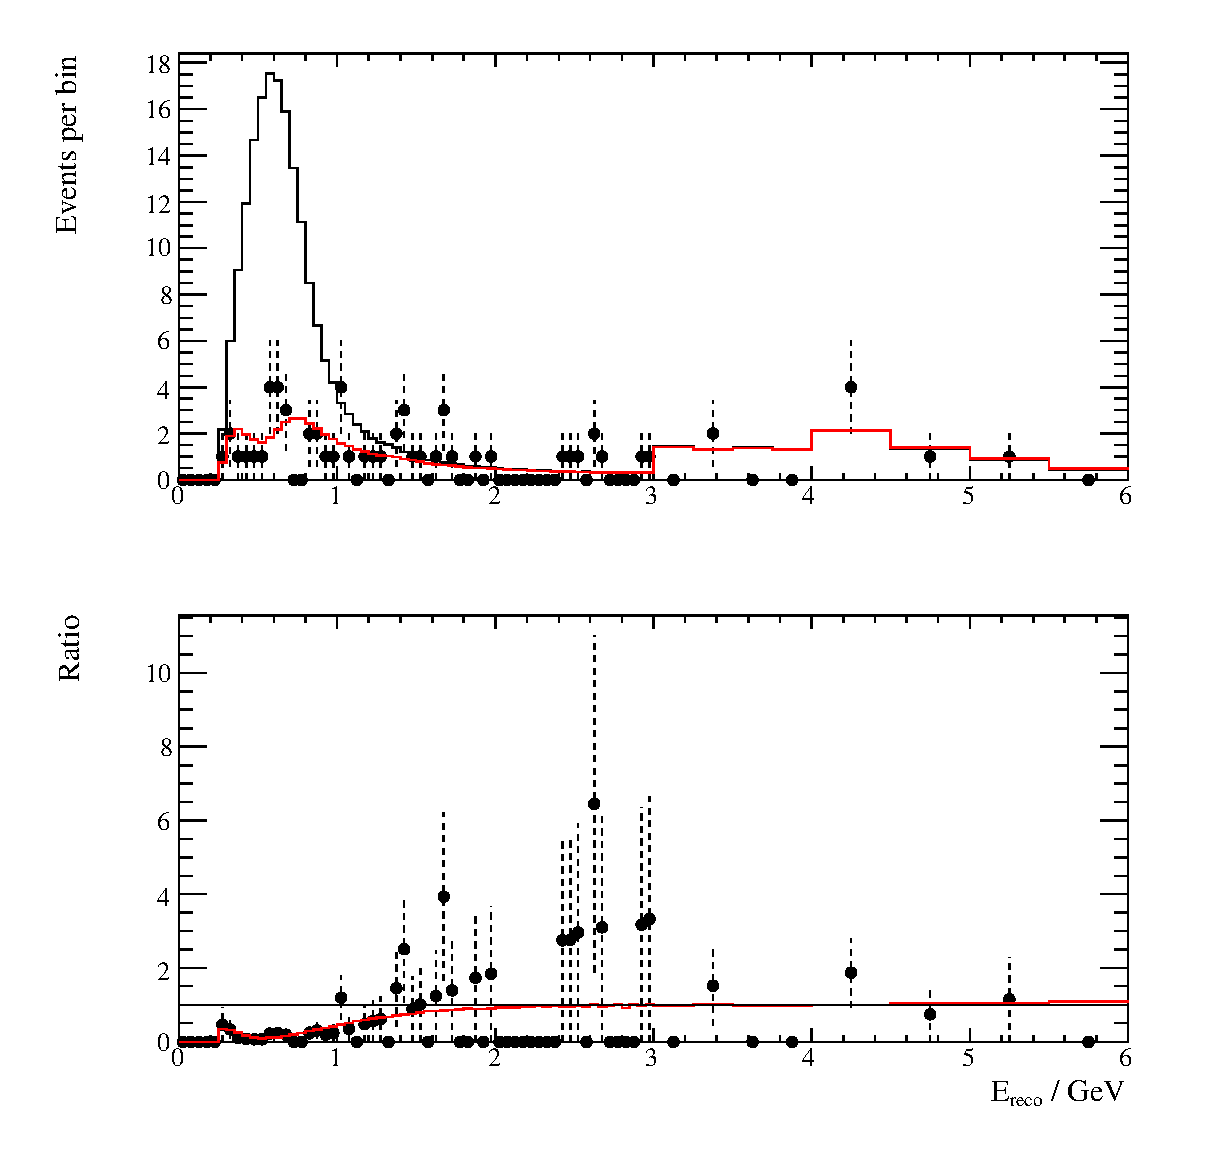
\includegraphics[width=15pc]{./images/fit_toymc/example_fits/spectrum_0}
\caption {
  Best-fit spectrum (top) and ratios of data and best-fit spectrum to predicted spectrum
  for no oscillations (bottom) for the 2+8 fit to fake data set 0
}
\label{fig:fakedata_spectrum_0}
\end{minipage}
\hspace{0.06\linewidth}
\begin{minipage}[t]{0.48\linewidth}
\center
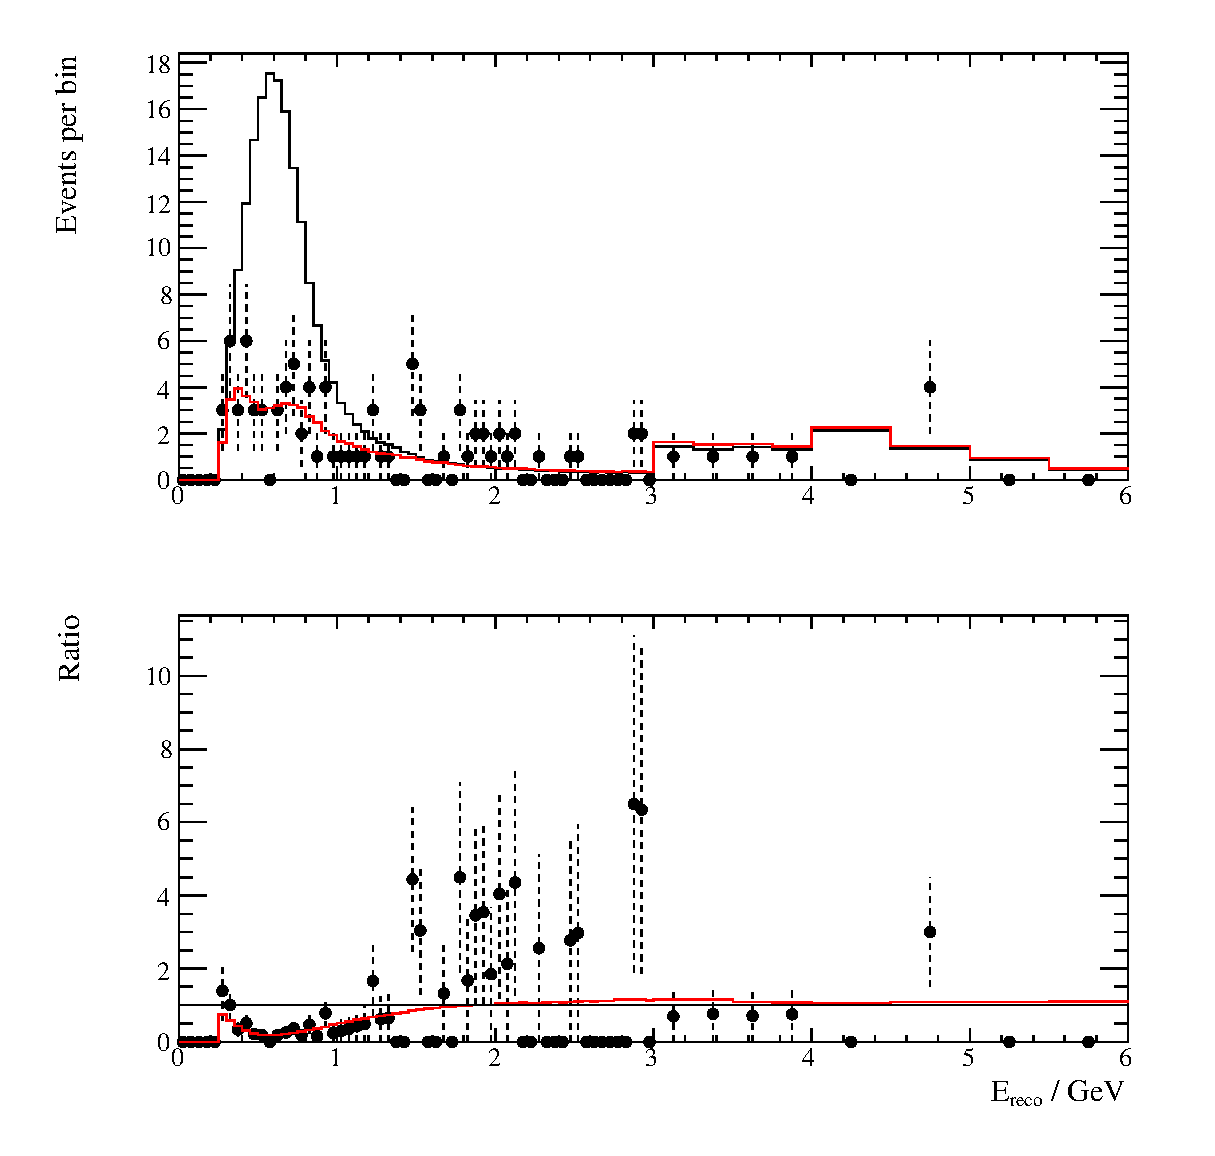
\includegraphics[width=15pc]{./images/fit_toymc/example_fits/spectrum_1}
\caption { 
  Best-fit spectrum (top) and ratios of data and best-fit spectrum to predicted spectrum
  for no oscillations (bottom) for the 2+8 fit to fake data set 1
}
\label{fig:fakedata_spectrum_1}
\end{minipage}
\vfill
\begin{minipage}[t]{0.48\linewidth}
\center
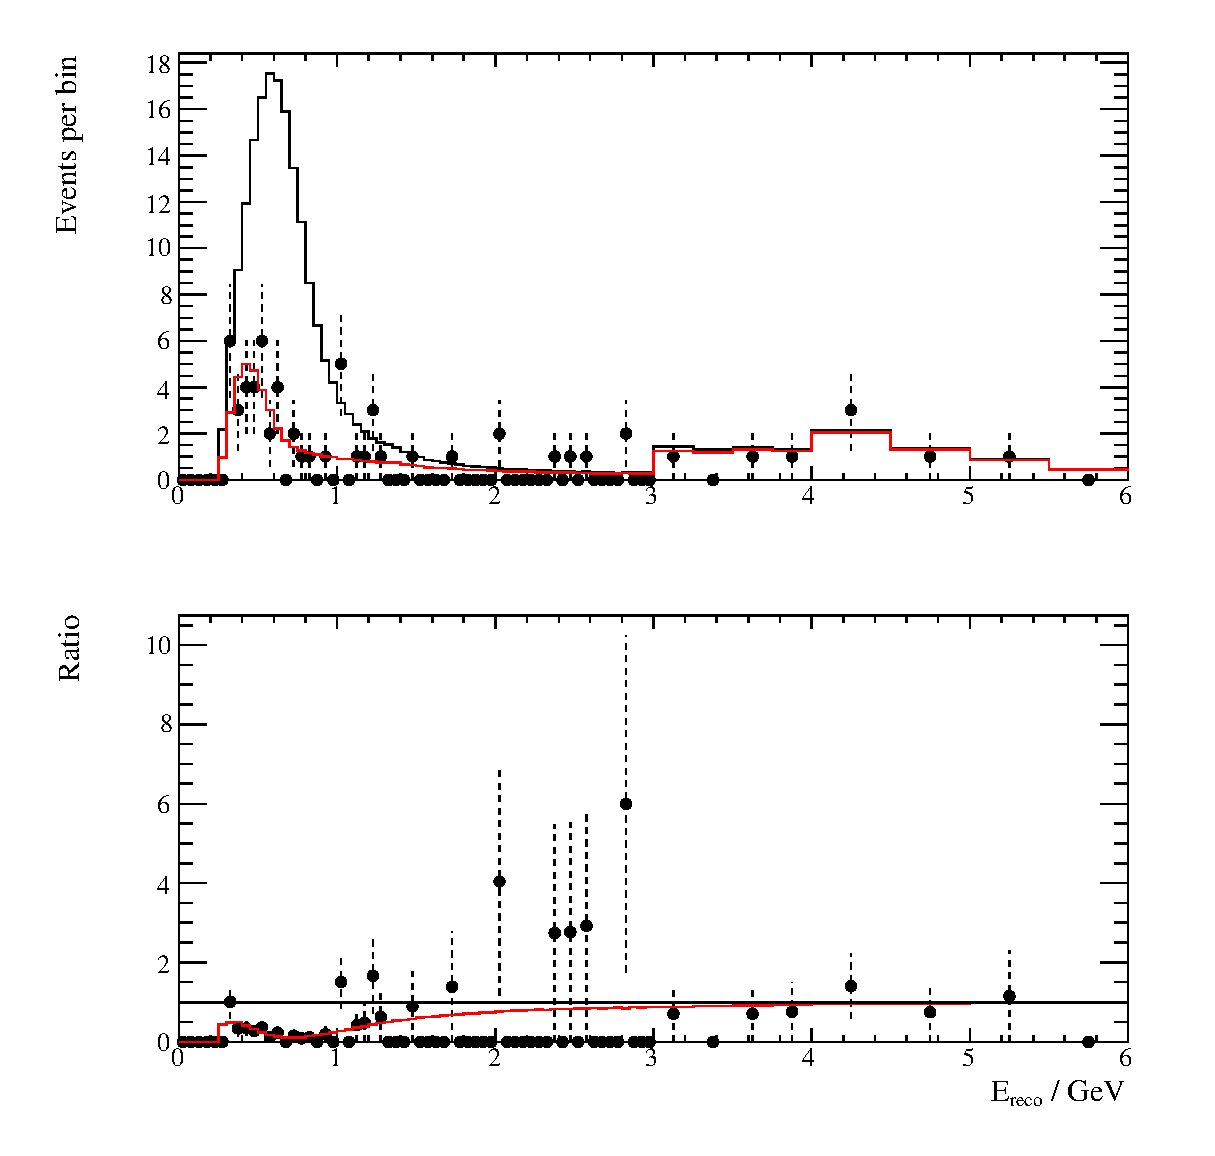
\includegraphics[width=15pc]{./images/fit_toymc/example_fits/spectrum_2}
\caption {
  Best-fit spectrum (top) and ratios of data and best-fit spectrum to predicted spectrum
  for no oscillations (bottom) for the 2+8 fit to fake data set 2
}
\label{fig:fakedata_spectrum_2}
\end{minipage}
\hspace{0.06\linewidth}
\begin{minipage}[t]{0.48\linewidth}
\center
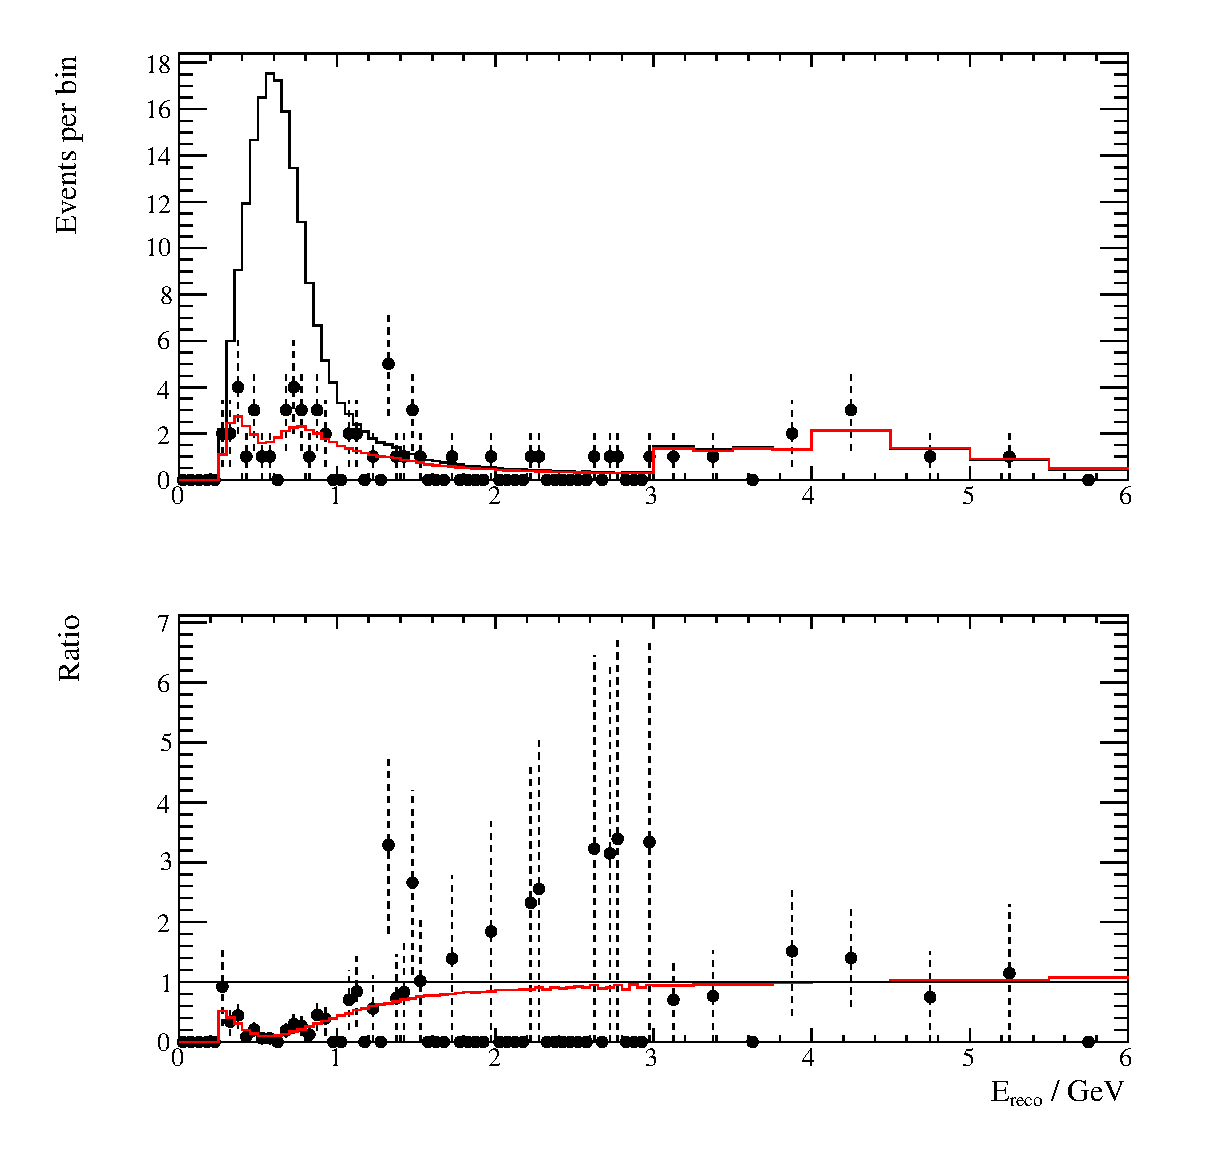
\includegraphics[width=15pc]{./images/fit_toymc/example_fits/spectrum_3}
\caption { 
  Best-fit spectrum (top) and ratios of data and best-fit spectrum to predicted spectrum
  for no oscillations (bottom) for the 2+8 fit to fake data set 3
}
\label{fig:fakedata_spectrum_3}
\end{minipage}
\vfill
\begin{minipage}[t]{0.48\linewidth}
\center
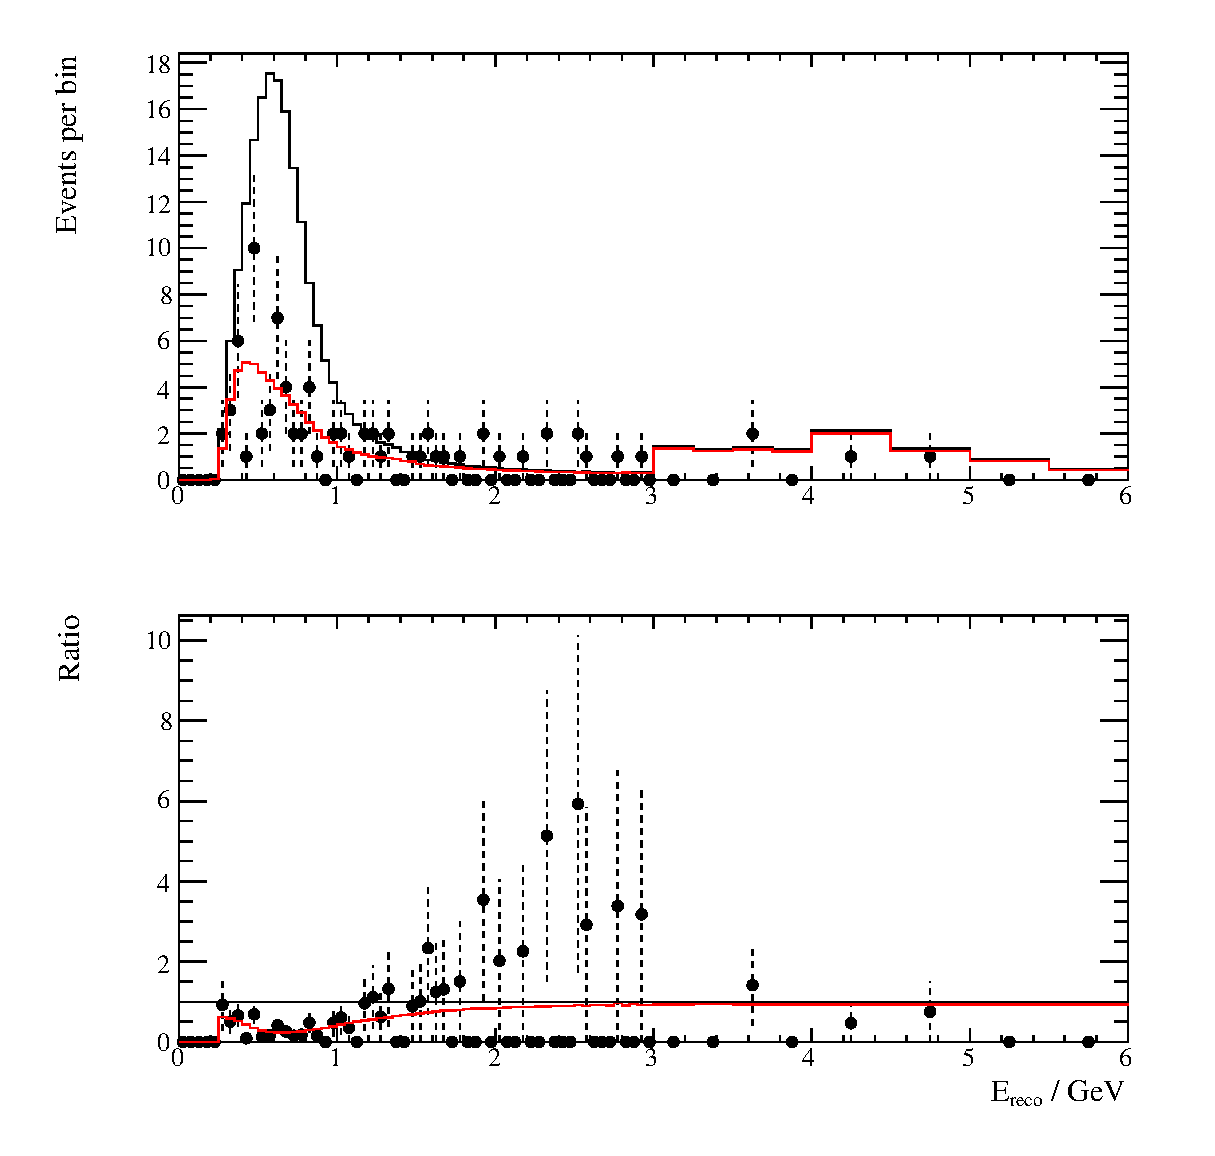
\includegraphics[width=15pc]{./images/fit_toymc/example_fits/spectrum_4}
\caption {
  Best-fit spectrum (top) and ratios of data and best-fit spectrum to predicted spectrum
  for no oscillations (bottom) for the 2+8 fit to fake data set 4
}
\label{fig:fakedata_spectrum_4}
\end{minipage}
\hspace{0.06\linewidth}
\begin{minipage}[t]{0.48\linewidth}
\center
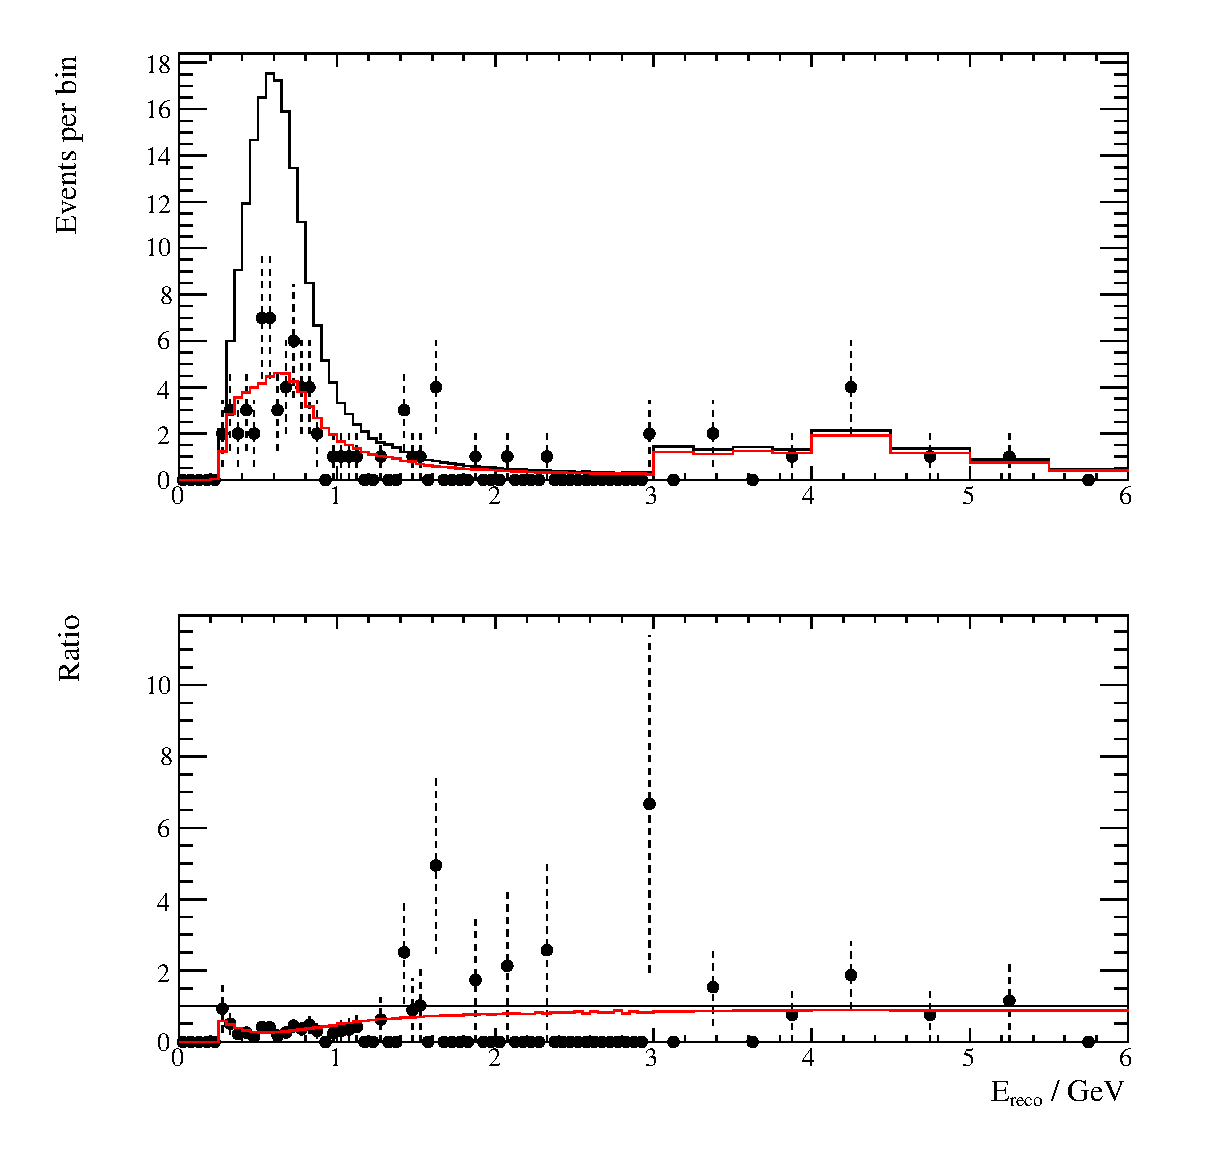
\includegraphics[width=15pc]{./images/fit_toymc/example_fits/spectrum_5}
\caption { 
  Best-fit spectrum (top) and ratios of data and best-fit spectrum to predicted spectrum
  for no oscillations (bottom) for the 2+8 fit to fake data set 5
}
\label{fig:fakedata_spectrum_5}
\end{minipage}
\end{figure*}

%...........................................................
%
% Best-fit spectra comparison comparing 2+8, 2+N and input
%

\begin{figure*}[htb]
\begin{minipage}[t]{0.48\linewidth}
\center
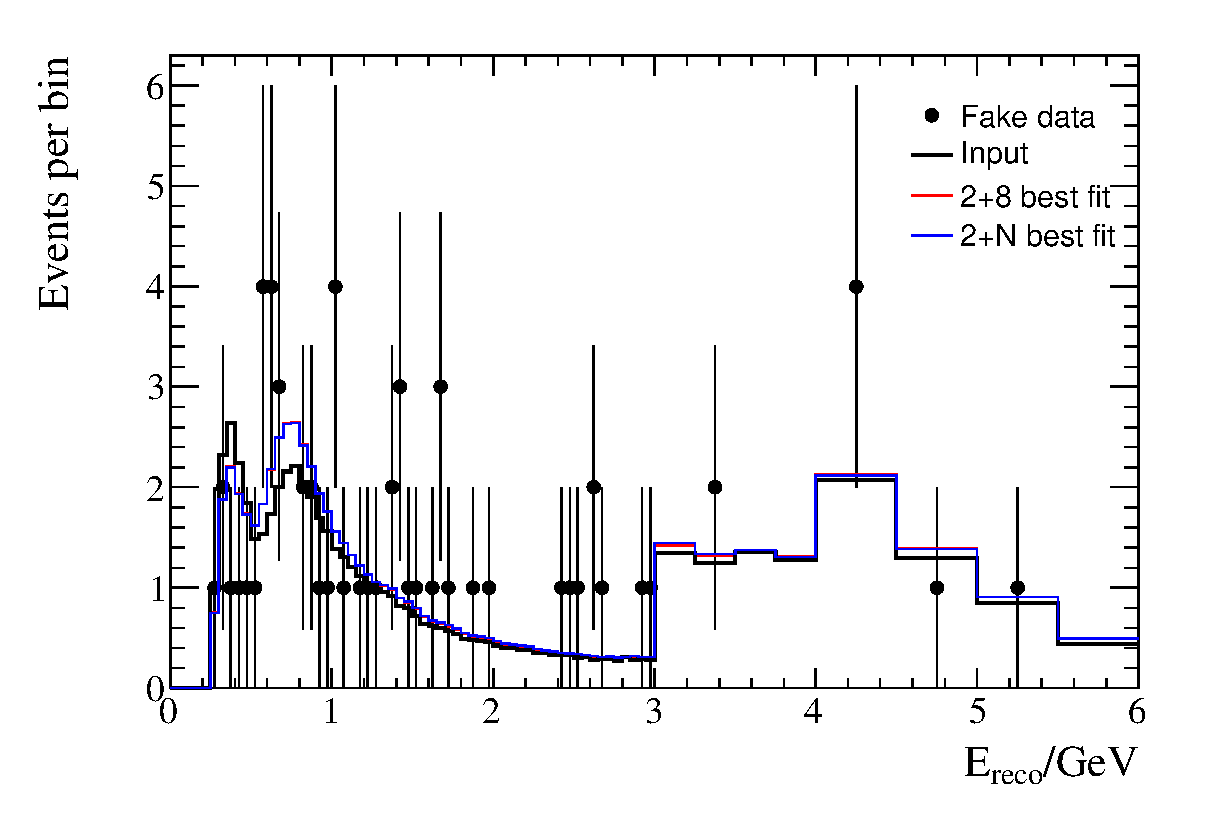
\includegraphics[width=18pc]{./images/fit_toymc/example_fits/fakedata_spectra_comparison_0}
\caption {
  Comparisons of the 2+8 and 2+N best-fit spectra with the input distribution for fake data set 0
}
\label{fig:fakedata_spectrum_comparison_0}
\end{minipage}
\hspace{0.06\linewidth}
\begin{minipage}[t]{0.48\linewidth}
\center
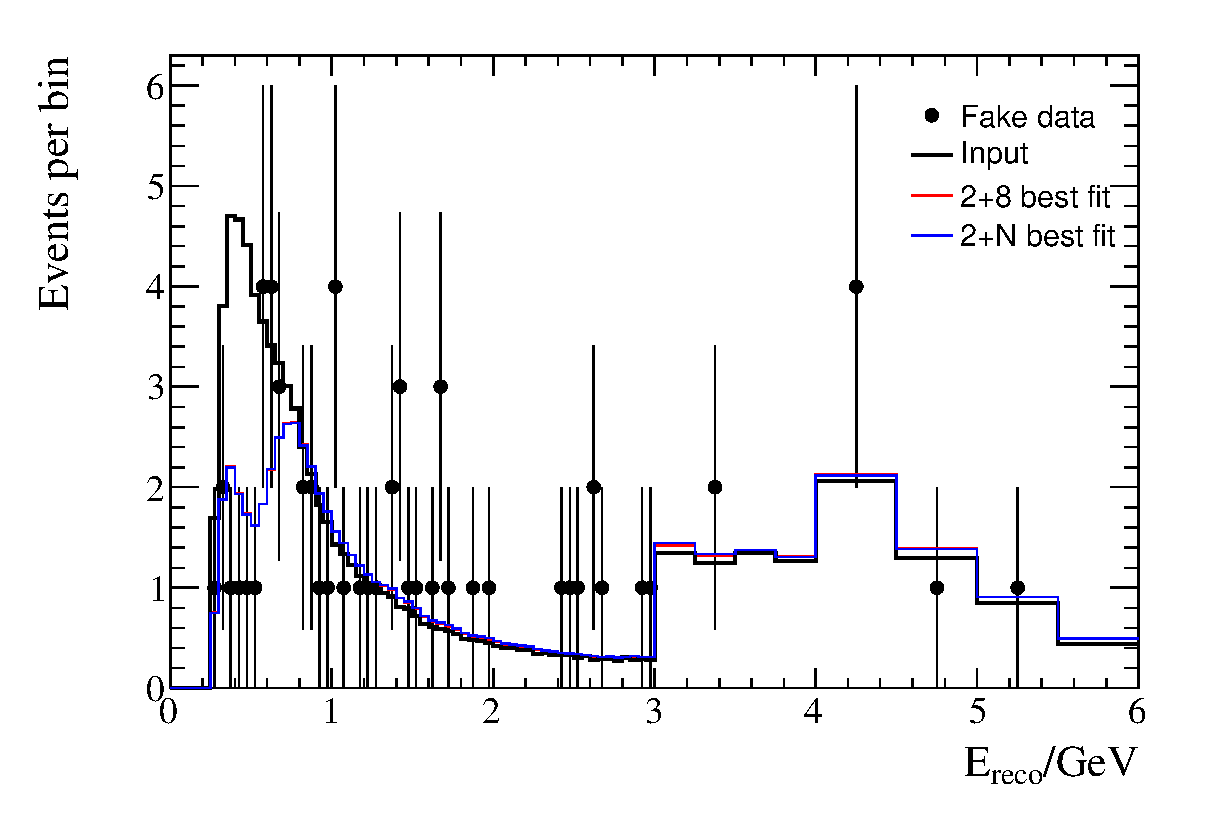
\includegraphics[width=18pc]{./images/fit_toymc/example_fits/fakedata_spectra_comparison_1}
\caption { 
  Comparisons of the 2+8 and 2+N best-fit spectra with the input distribution for fake data set 1
}
\label{fig:fakedata_spectrum_comparison_1}
\end{minipage}
\vfill
\begin{minipage}[t]{0.48\linewidth}
\center
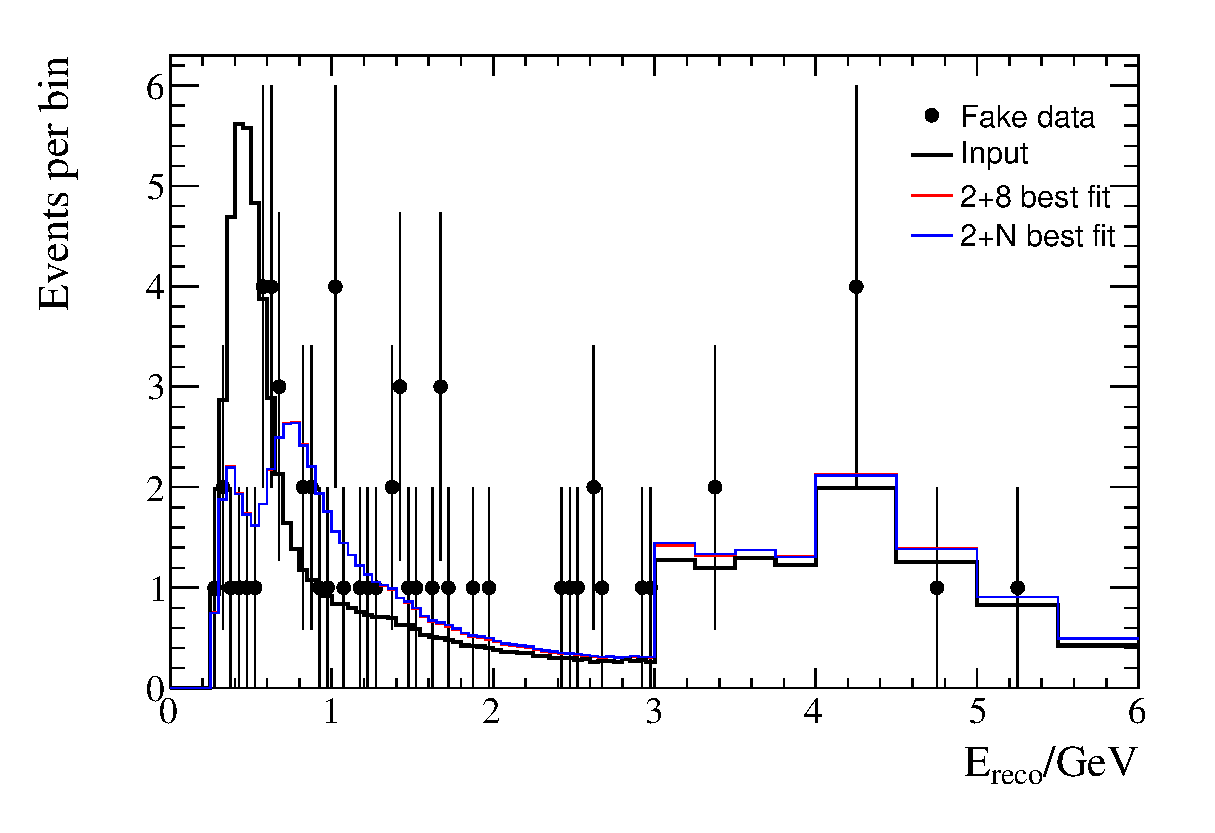
\includegraphics[width=18pc]{./images/fit_toymc/example_fits/fakedata_spectra_comparison_2}
\caption {
  Comparisons of the 2+8 and 2+N best-fit spectra with the input distribution for fake data set 2
}
\label{fig:fakedata_spectrum_comparison_2}
\end{minipage}
\hspace{0.06\linewidth}
\begin{minipage}[t]{0.48\linewidth}
\center
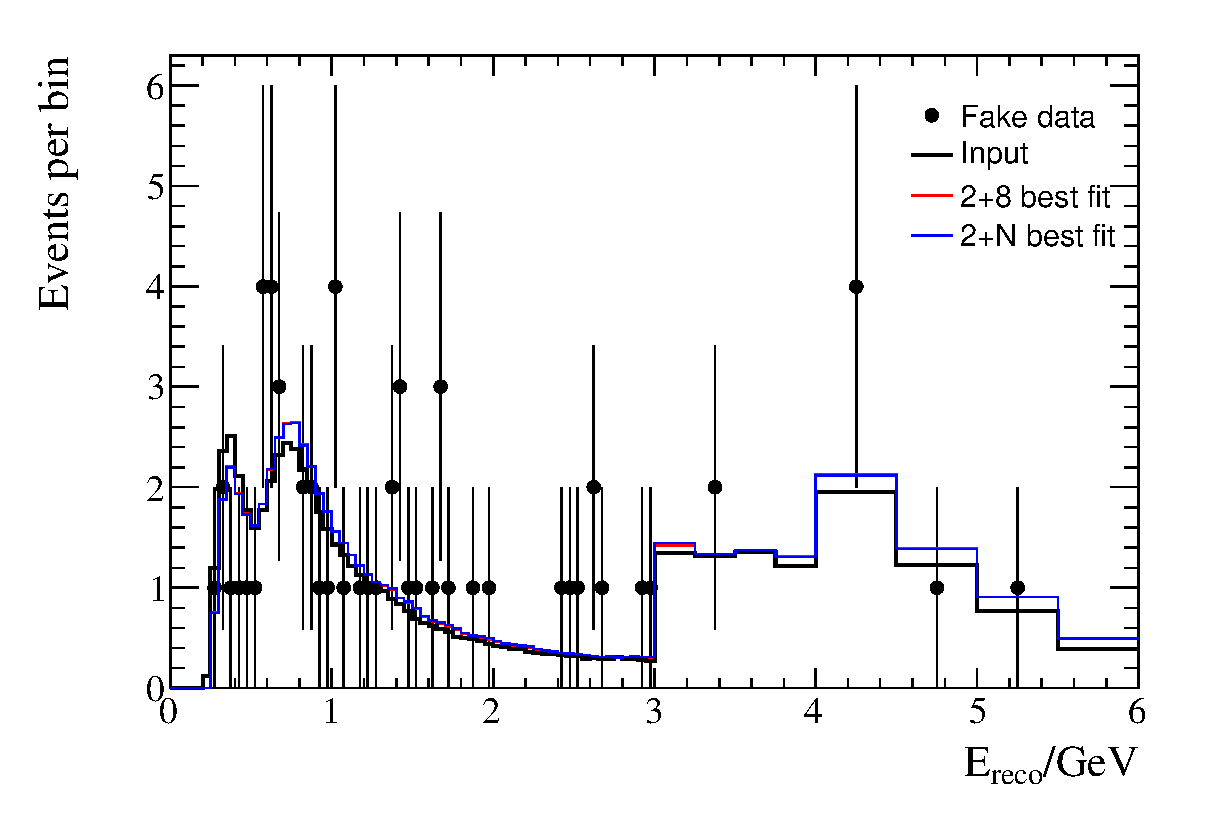
\includegraphics[width=18pc]{./images/fit_toymc/example_fits/fakedata_spectra_comparison_3}
\caption { 
  Comparisons of the 2+8 and 2+N best-fit spectra with the input distribution for fake data set 3
}
\label{fig:fakedata_spectrum_comparison_3}
\end{minipage}
\vfill
\begin{minipage}[t]{0.48\linewidth}
\center
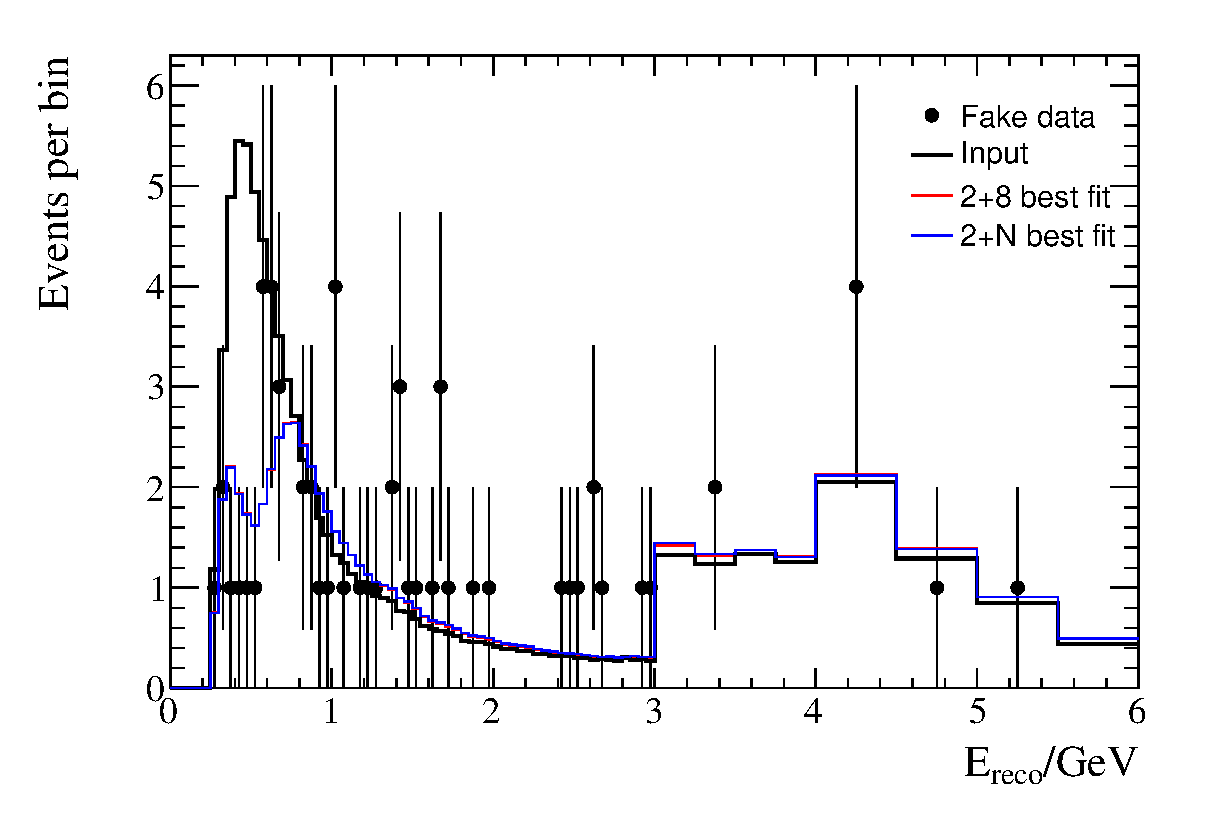
\includegraphics[width=18pc]{./images/fit_toymc/example_fits/fakedata_spectra_comparison_4}
\caption {
  Comparisons of the 2+8 and 2+N best-fit spectra with the input distribution for fake data set 4
}
\label{fig:fakedata_spectrum_comparison_4}
\end{minipage}
\hspace{0.06\linewidth}
\begin{minipage}[t]{0.48\linewidth}
\center
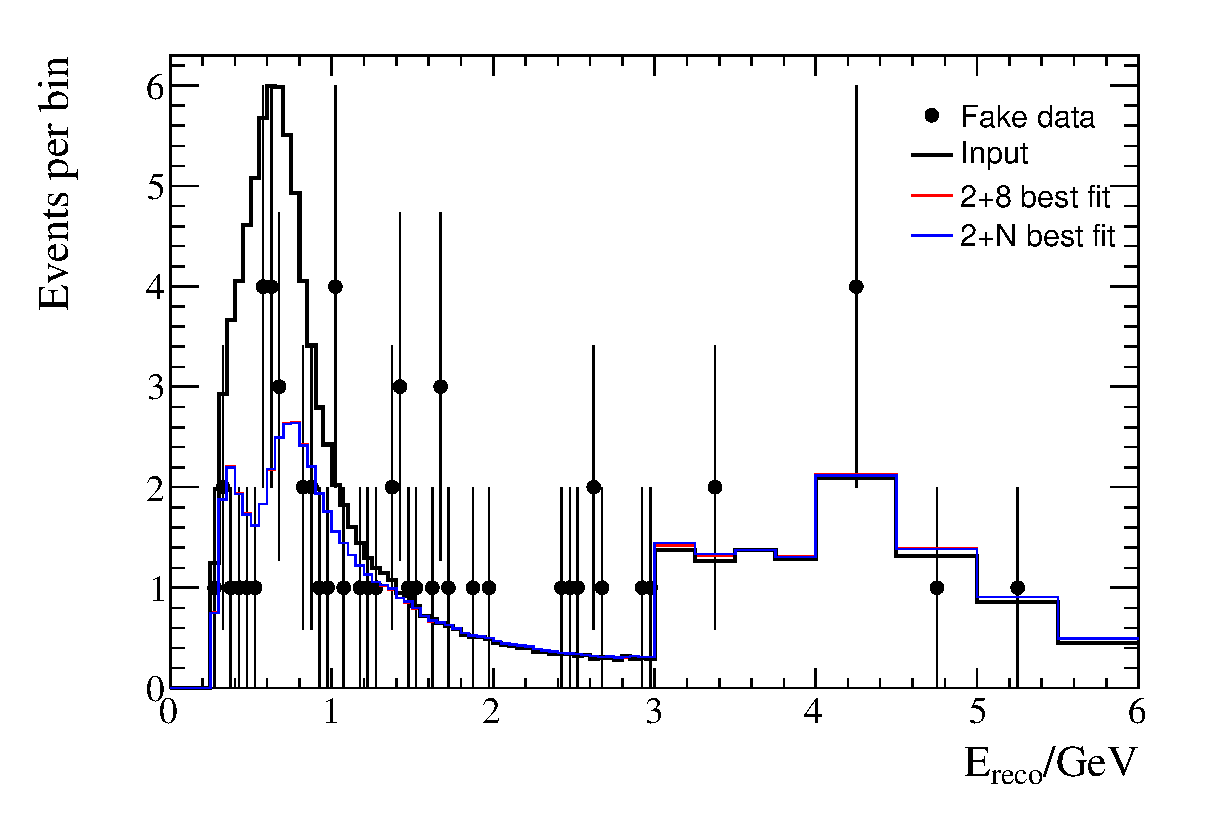
\includegraphics[width=18pc]{./images/fit_toymc/example_fits/fakedata_spectra_comparison_5}
\caption { 
  Comparisons of the 2+8 and 2+N best-fit spectra with the input distribution for fake data set 5
}
\label{fig:fakedata_spectrum_comparison_5}
\end{minipage}
\end{figure*}

\clearpage
\subsection{$\Delta\chi^2$ surfaces}
\label{appendix:example_toy_mc_fits:dchisq}

%...........................................................
%
% dchisq surfaces for `2+N' fits
%

\begin{figure*}[htb]
\begin{minipage}[t]{0.48\linewidth}
\center
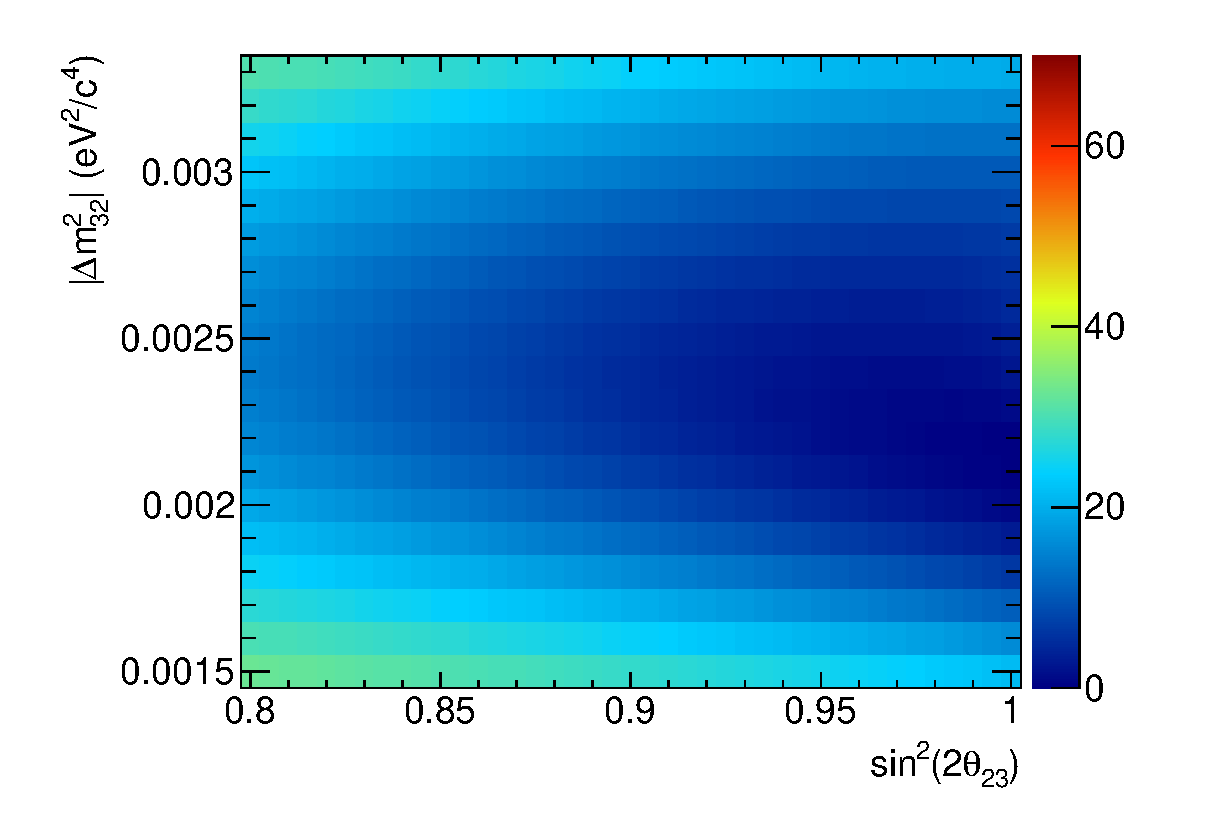
\includegraphics[width=18pc]{./images/fit_toymc/example_fits/2N/dchisq_0}
\caption {
  $\Delta\chi^2$ surface for the 2+N fit to fake data set 0
}
\label{fig:fakedata_chisq_2N_0}
\end{minipage}
\hspace{0.06\linewidth}
\begin{minipage}[t]{0.48\linewidth}
\center
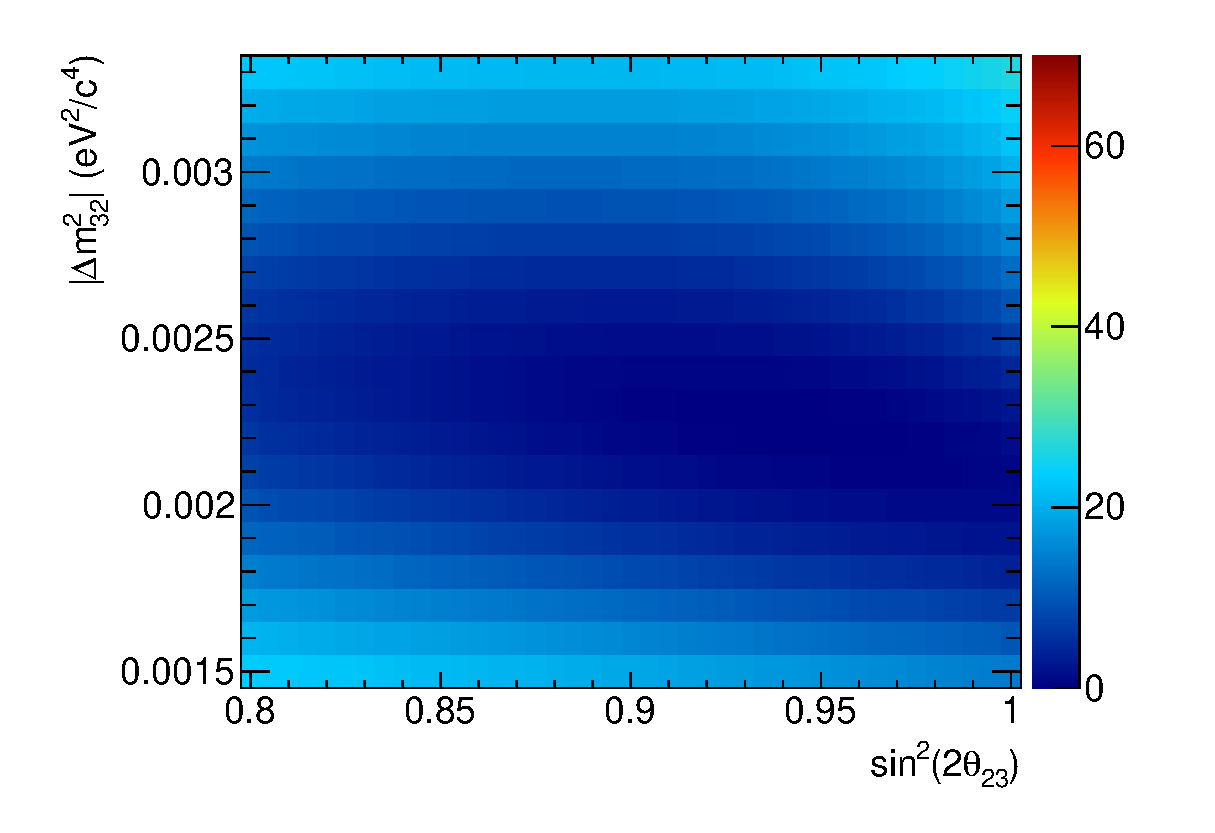
\includegraphics[width=18pc]{./images/fit_toymc/example_fits/2N/dchisq_1}
\caption { 
  $\Delta\chi^2$ surface for the 2+N fit to fake data set 1
}
\label{fig:fakedata_chisq_2N_1}
\end{minipage}
\vfill
\begin{minipage}[t]{0.48\linewidth}
\center
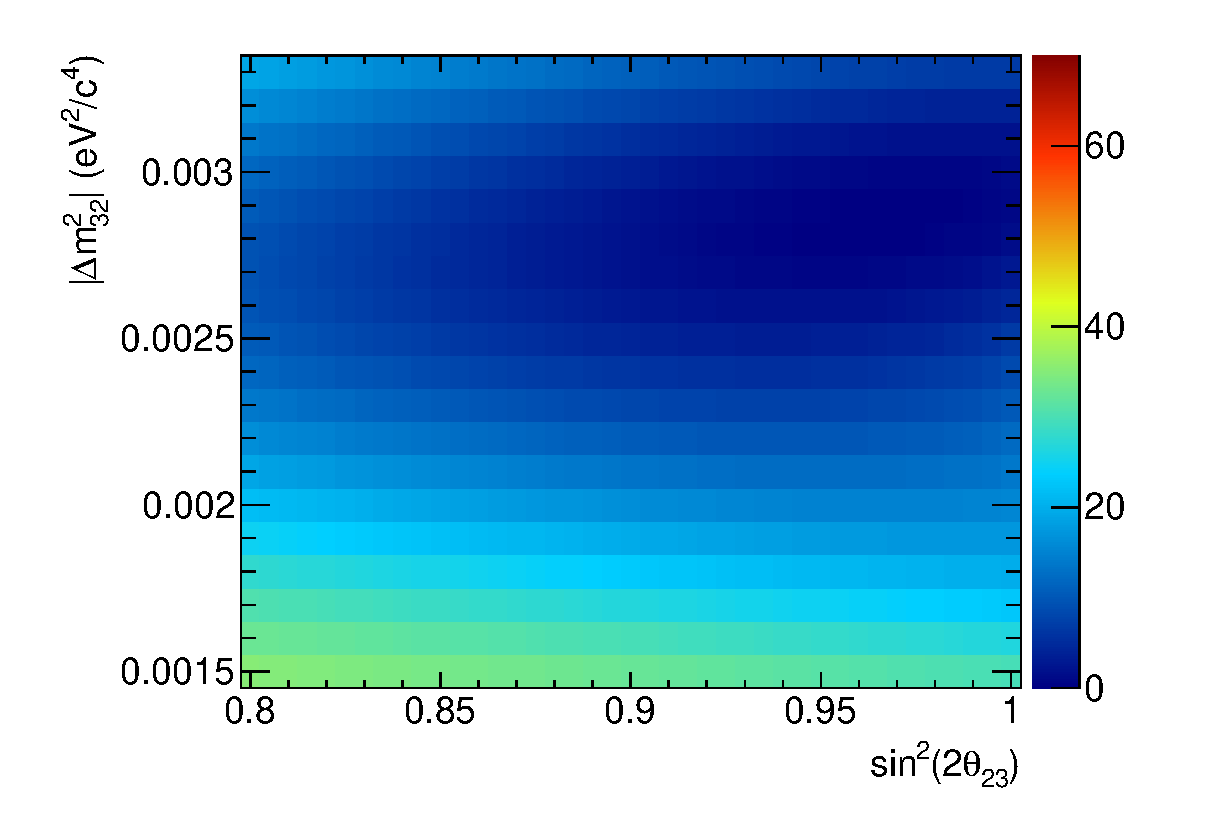
\includegraphics[width=18pc]{./images/fit_toymc/example_fits/2N/dchisq_2}
\caption {
  $\Delta\chi^2$ surface for the 2+N fit to fake data set 2
}
\label{fig:fakedata_chisq_2N_2}
\end{minipage}
\hspace{0.06\linewidth}
\begin{minipage}[t]{0.48\linewidth}
\center
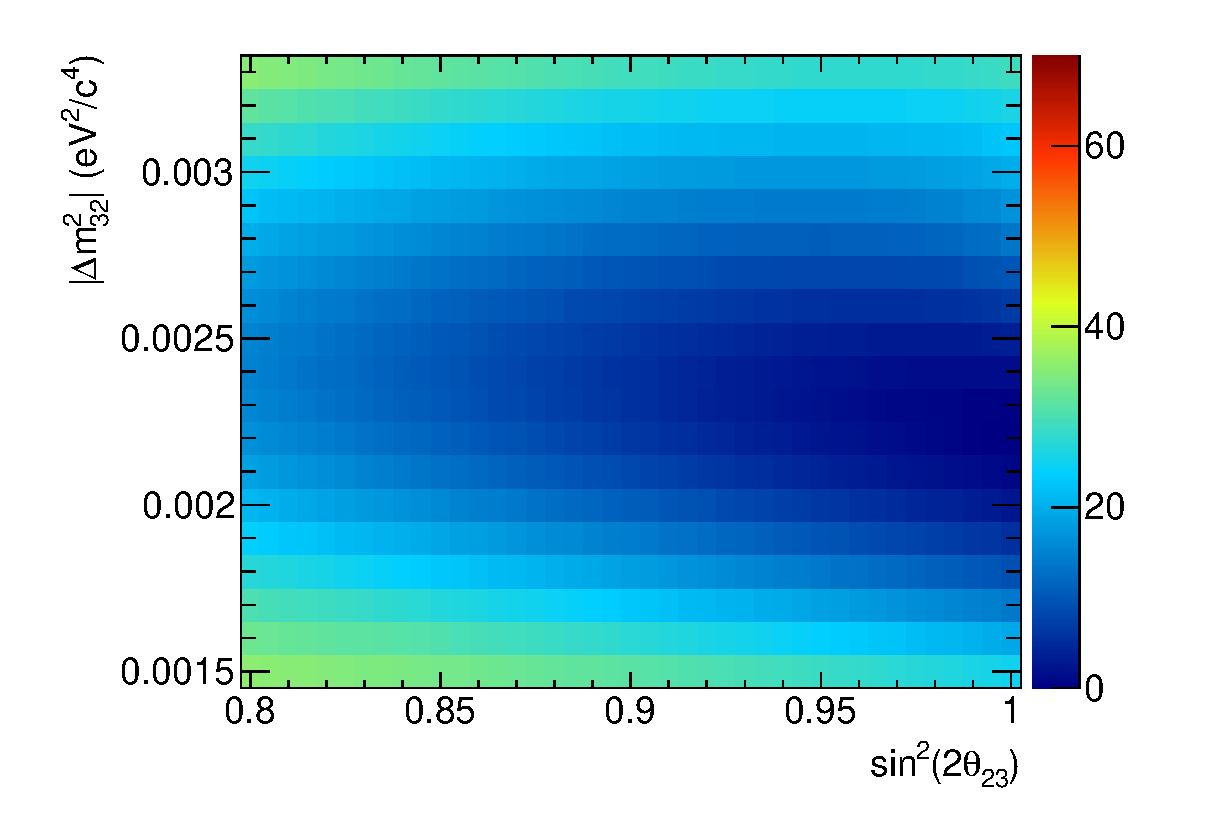
\includegraphics[width=18pc]{./images/fit_toymc/example_fits/2N/dchisq_3}
\caption { 
  $\Delta\chi^2$ surface for the 2+N fit to fake data set 3
}
\label{fig:fakedata_chisq_2N_3}
\end{minipage}
\vfill
\begin{minipage}[t]{0.48\linewidth}
\center
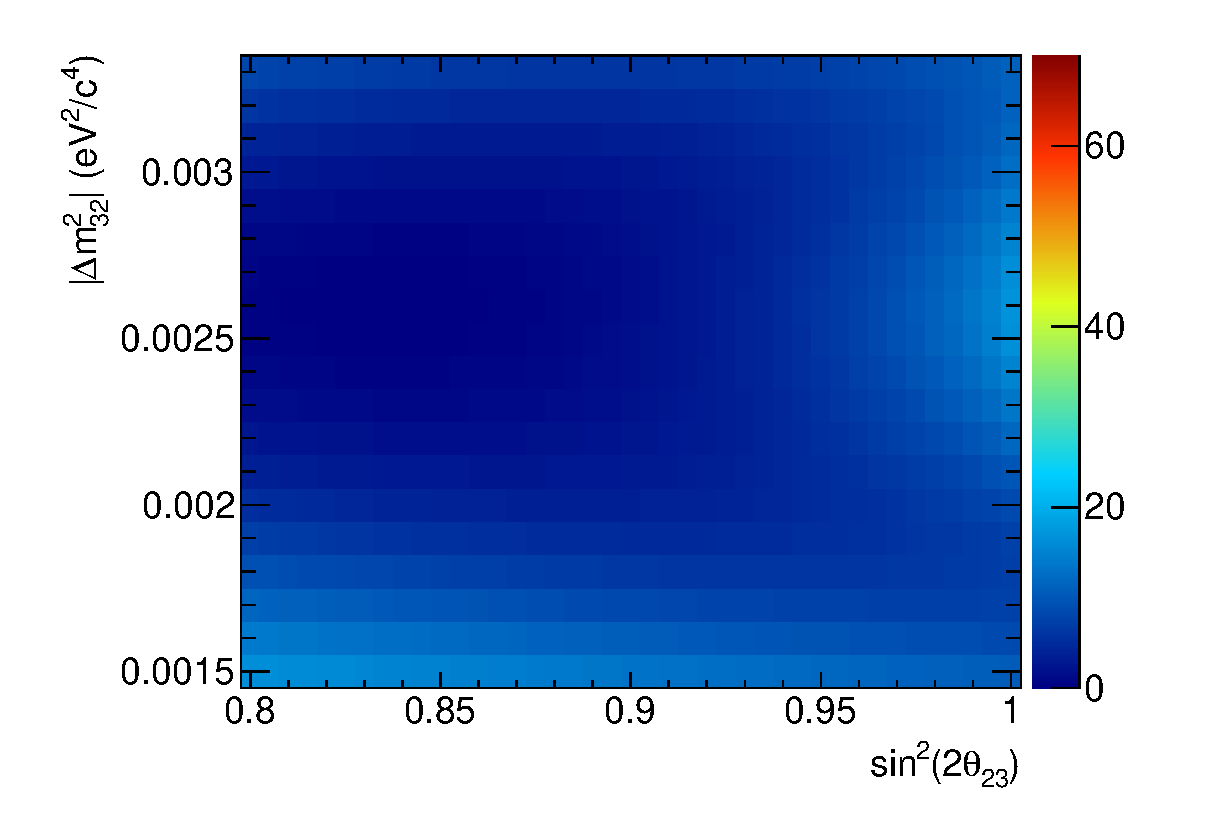
\includegraphics[width=18pc]{./images/fit_toymc/example_fits/2N/dchisq_4}
\caption {
  $\Delta\chi^2$ surface for the 2+N fit to fake data set 4
}
\label{fig:fakedata_chisq_2N_4}
\end{minipage}
\hspace{0.06\linewidth}
\begin{minipage}[t]{0.48\linewidth}
\center
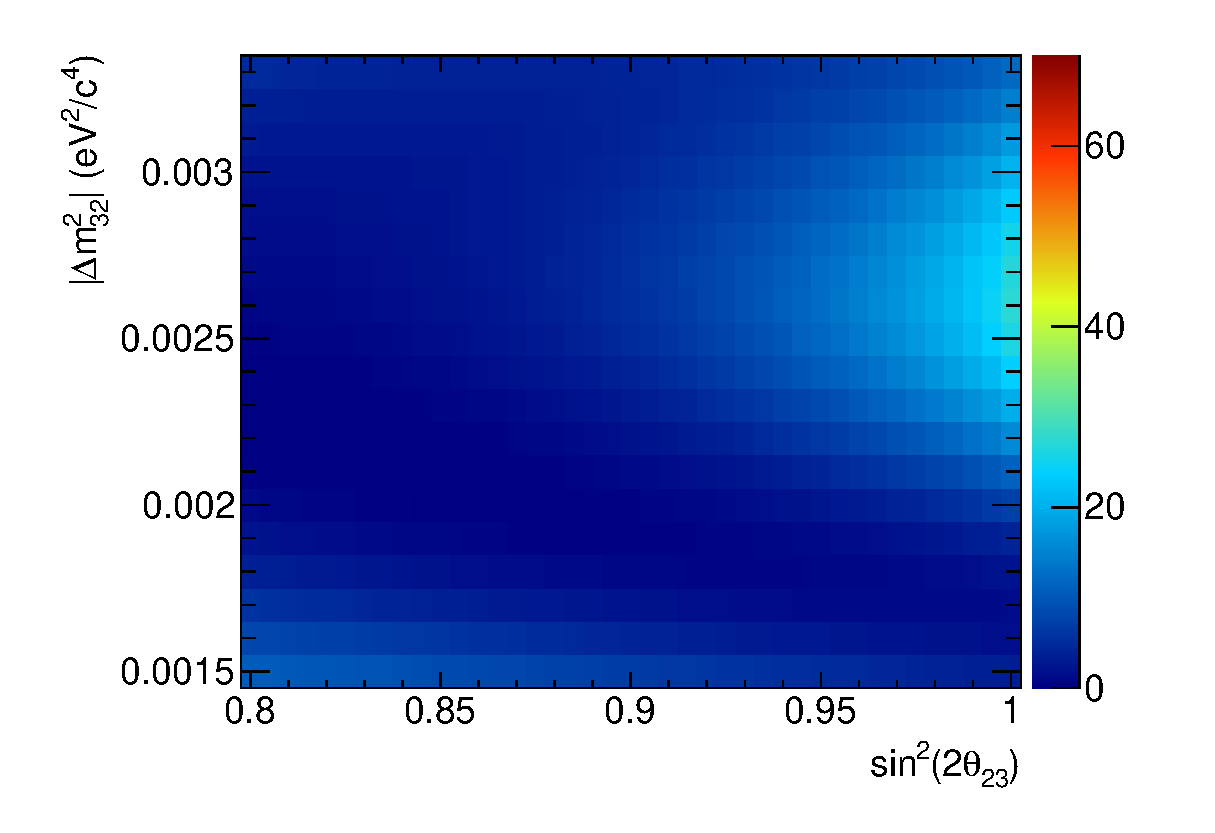
\includegraphics[width=18pc]{./images/fit_toymc/example_fits/2N/dchisq_5}
\caption { 
  $\Delta\chi^2$ surface for the 2+N fit to fake data set 5
}
\label{fig:fakedata_chisq_2N_5}
\end{minipage}
\end{figure*}

%...........................................................
%
% dchisq surfaces for `2+8' fits
%

\begin{figure*}[htb]
\begin{minipage}[t]{0.48\linewidth}
\center
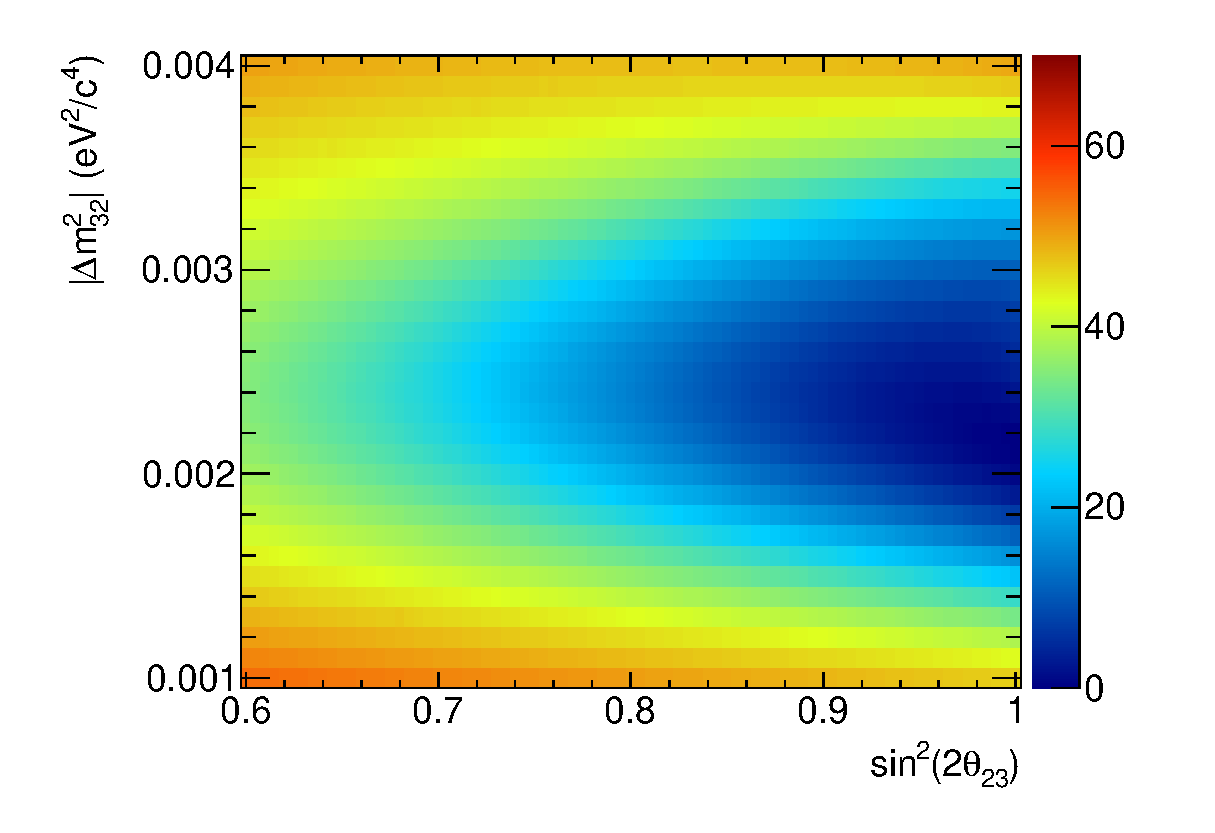
\includegraphics[width=18pc]{./images/fit_toymc/example_fits/dchisq_0}
\caption {
  $\Delta\chi^2$ surface for the 2+8 fit to fake data set 0
}
\label{fig:fakedata_chisq_0}
\end{minipage}
\hspace{0.06\linewidth}
\begin{minipage}[t]{0.48\linewidth}
\center
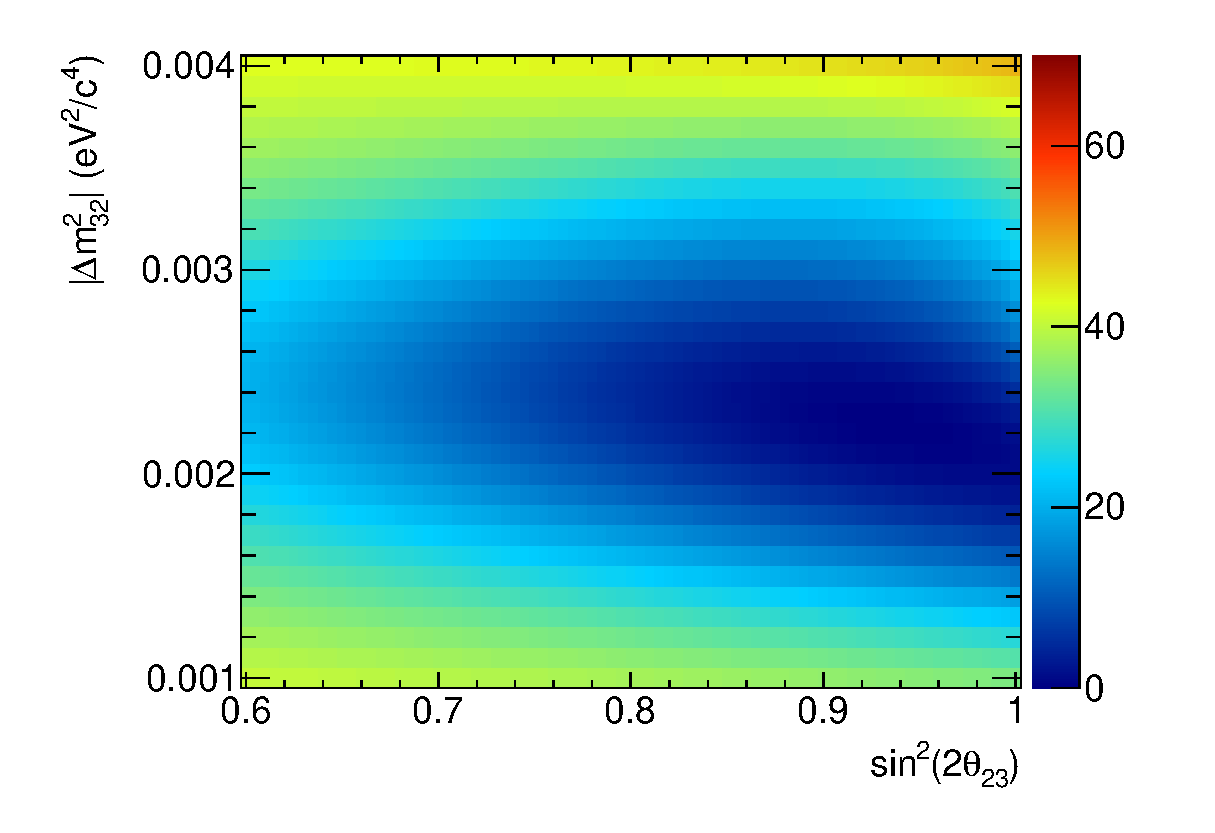
\includegraphics[width=18pc]{./images/fit_toymc/example_fits/dchisq_1}
\caption { 
  $\Delta\chi^2$ surface for the 2+8 fit to fake data set 1
}
\label{fig:fakedata_chisq_1}
\end{minipage}
\vfill
\begin{minipage}[t]{0.48\linewidth}
\center
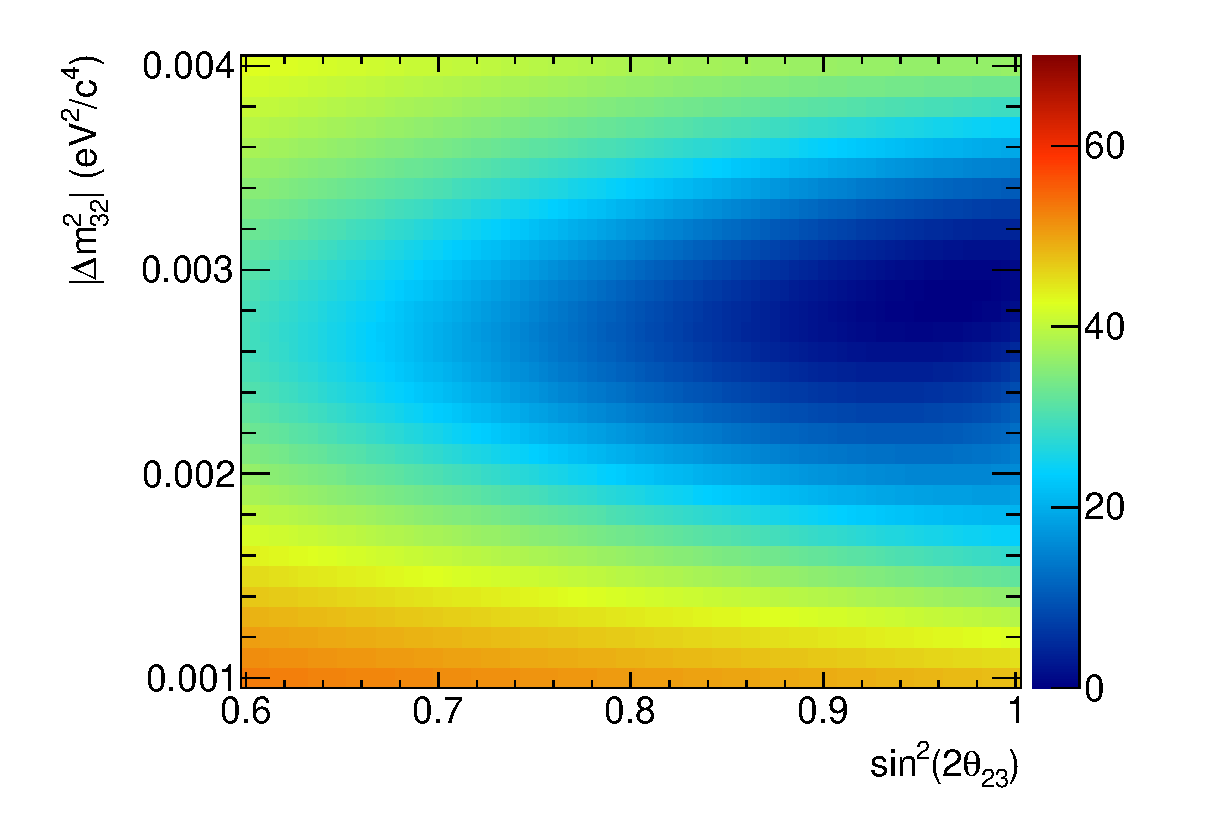
\includegraphics[width=18pc]{./images/fit_toymc/example_fits/dchisq_2}
\caption {
  $\Delta\chi^2$ surface for the 2+8 fit to fake data set 2
}
\label{fig:fakedata_chisq_2}
\end{minipage}
\hspace{0.06\linewidth}
\begin{minipage}[t]{0.48\linewidth}
\center
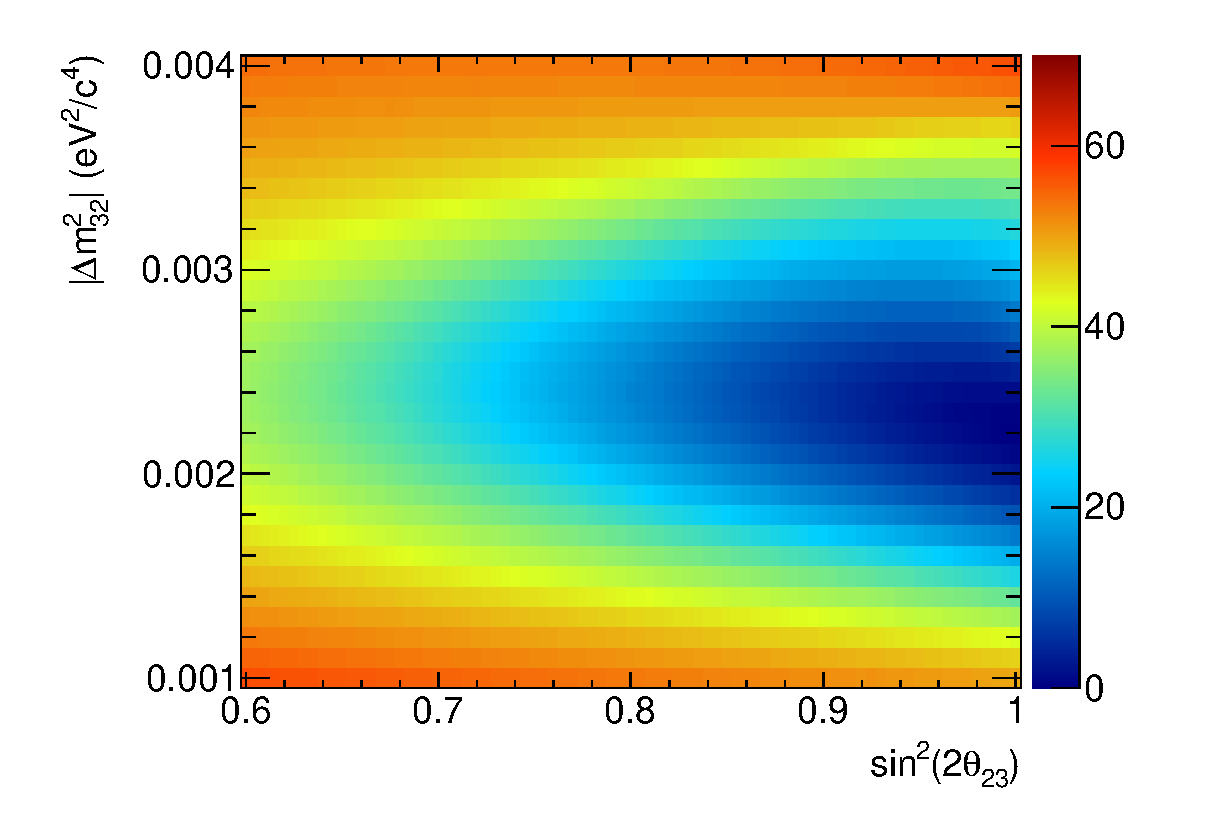
\includegraphics[width=18pc]{./images/fit_toymc/example_fits/dchisq_3}
\caption { 
  $\Delta\chi^2$ surface for the 2+8 fit to fake data set 3
}
\label{fig:fakedata_chisq_3}
\end{minipage}
\vfill
\begin{minipage}[t]{0.48\linewidth}
\center
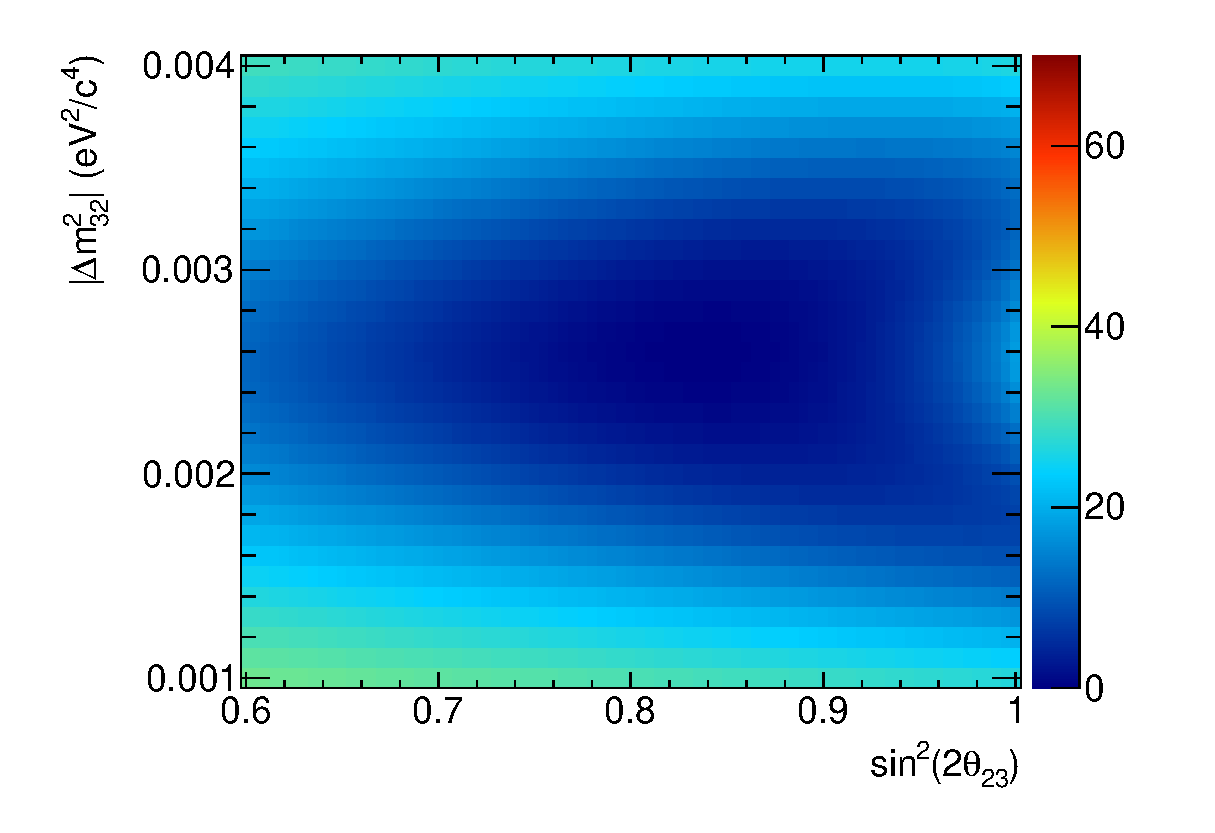
\includegraphics[width=18pc]{./images/fit_toymc/example_fits/dchisq_4}
\caption {
  $\Delta\chi^2$ surface, for the 2+8 fit to fake data set 4
}
\label{fig:fakedata_chisq_4}
\end{minipage}
\hspace{0.06\linewidth}
\begin{minipage}[t]{0.48\linewidth}
\center
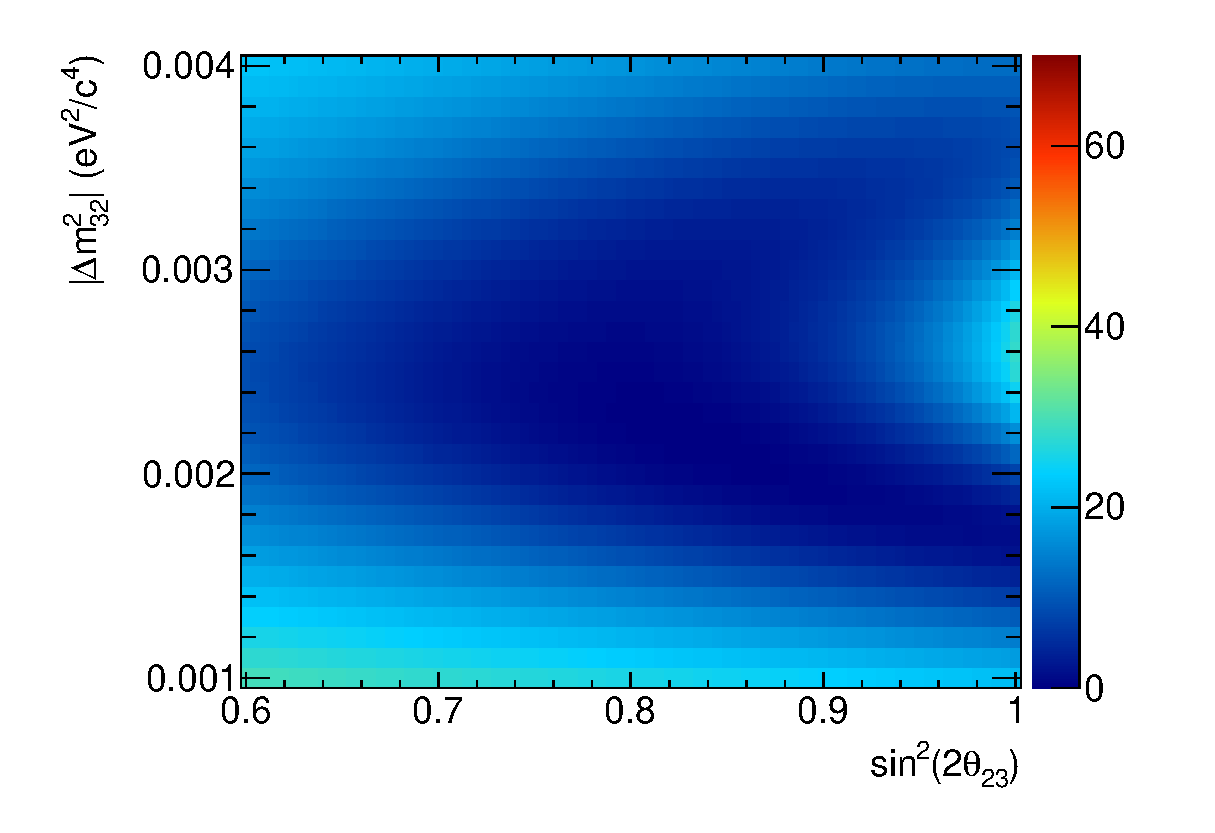
\includegraphics[width=18pc]{./images/fit_toymc/example_fits/dchisq_5}
\caption { 
  $\Delta\chi^2$ surface for the 2+8 fit to fake data set 5
}
\label{fig:fakedata_chisq_5}
\end{minipage}
\end{figure*}


\clearpage
\subsection{Contours}
\label{appendix:example_toy_mc_fits:contours}


%...........................................................
%
% Contours for `2+N' fits
%

\begin{figure*}[htb]
\begin{minipage}[t]{0.48\linewidth}
\center
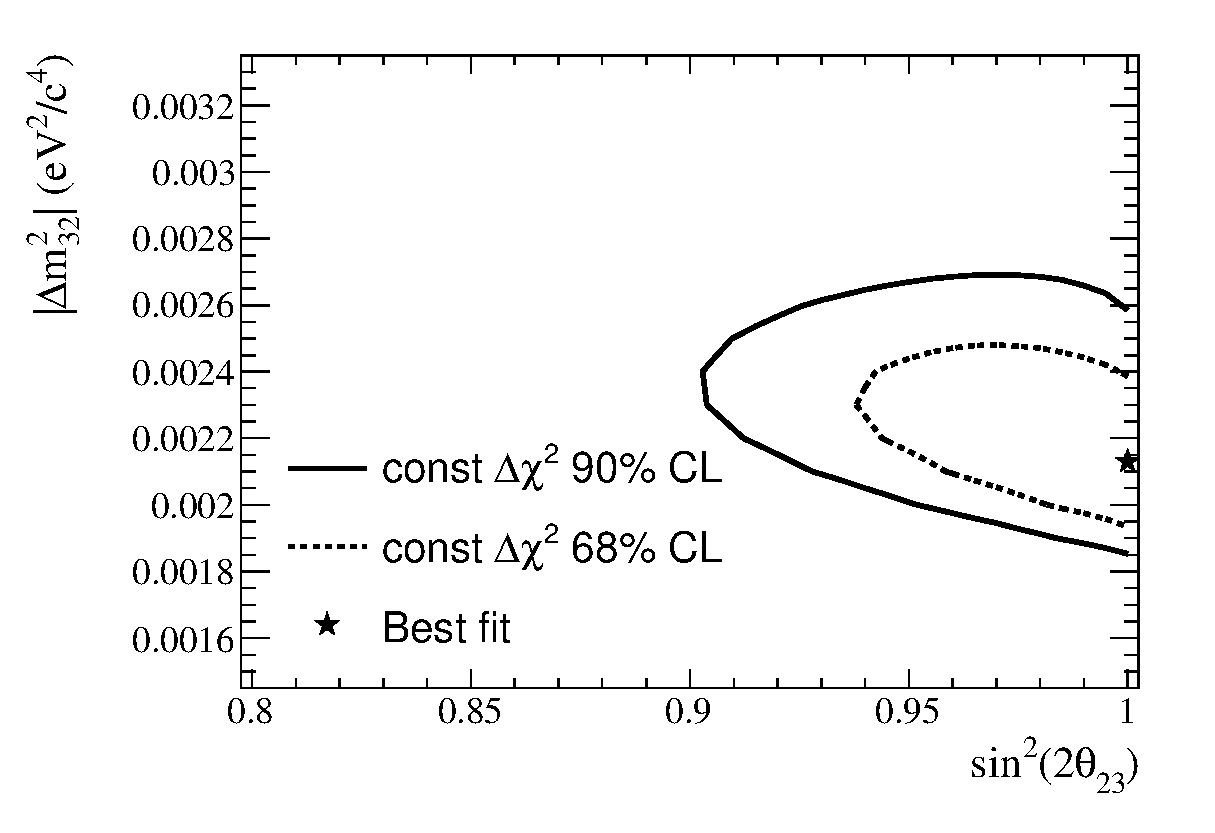
\includegraphics[width=18pc]{./images/fit_toymc/example_fits/2N/contours_0}
\caption {
  68\% and 90\% confidence regions for the 2+N fit to fake data set 0
}
\label{fig:fakedata_contours_2N_0}
\end{minipage}
\hspace{0.06\linewidth}
\begin{minipage}[t]{0.48\linewidth}
\center
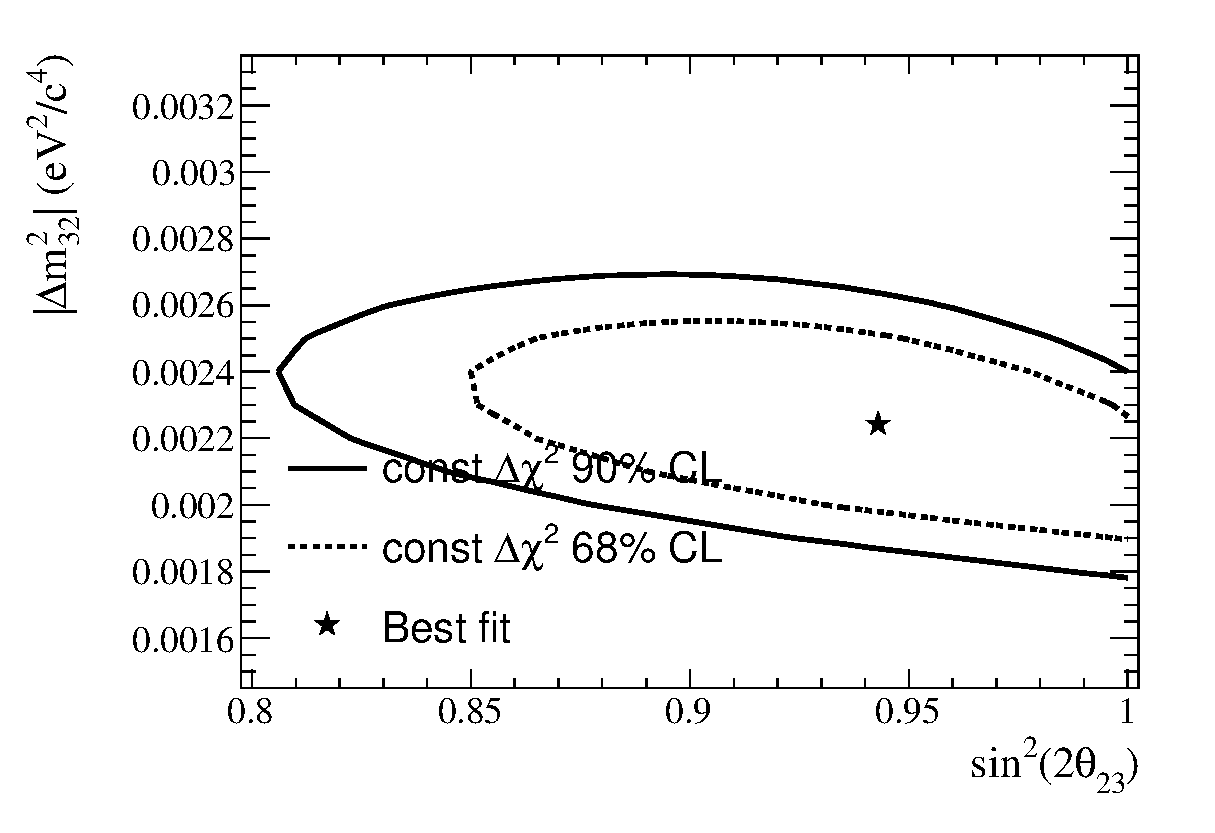
\includegraphics[width=18pc]{./images/fit_toymc/example_fits/2N/contours_1}
\caption { 
  68\% and 90\% confidence regions for the 2+N fit to fake data set 1
}
\label{fig:fakedata_contours_2N_1}
\end{minipage}
\vfill
\begin{minipage}[t]{0.48\linewidth}
\center
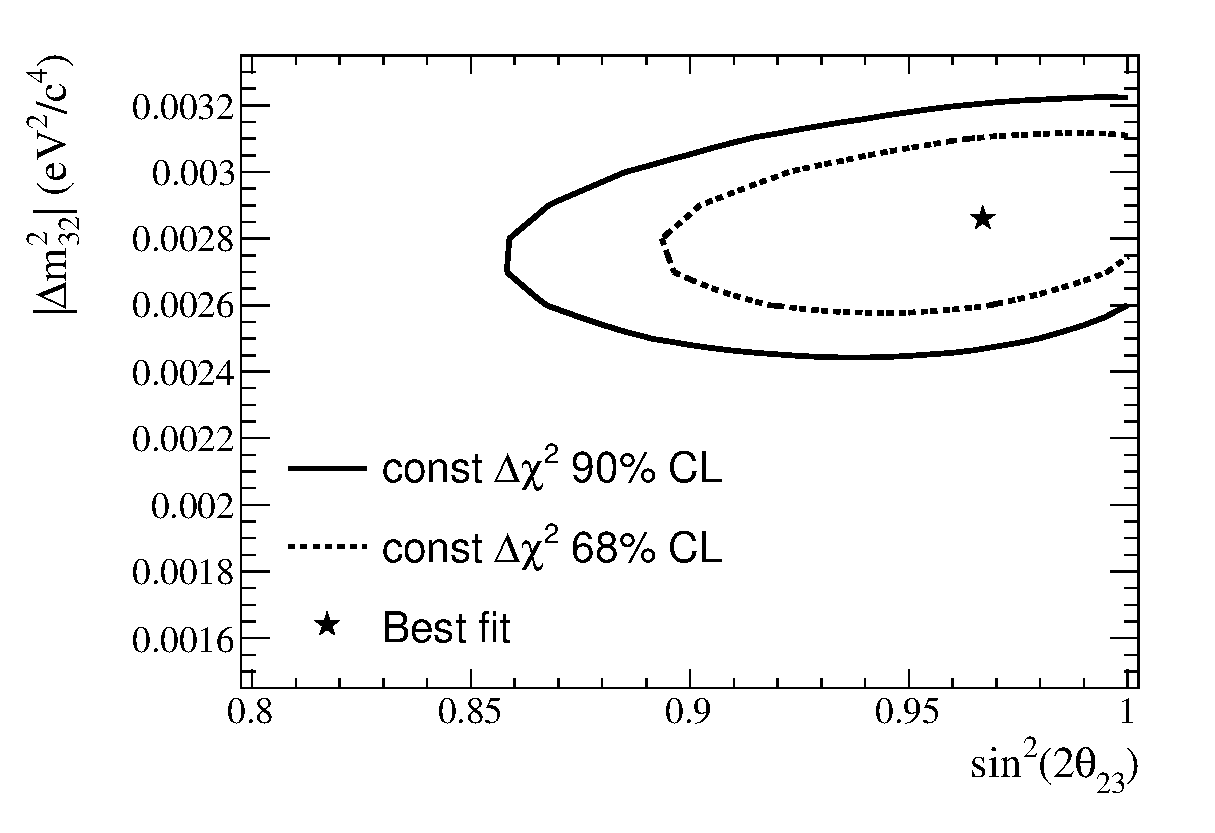
\includegraphics[width=18pc]{./images/fit_toymc/example_fits/2N/contours_2}
\caption {
  68\% and 90\% confidence regions for the 2+N fit to fake data set 2
}
\label{fig:fakedata_contours_2N_2}
\end{minipage}
\hspace{0.06\linewidth}
\begin{minipage}[t]{0.48\linewidth}
\center
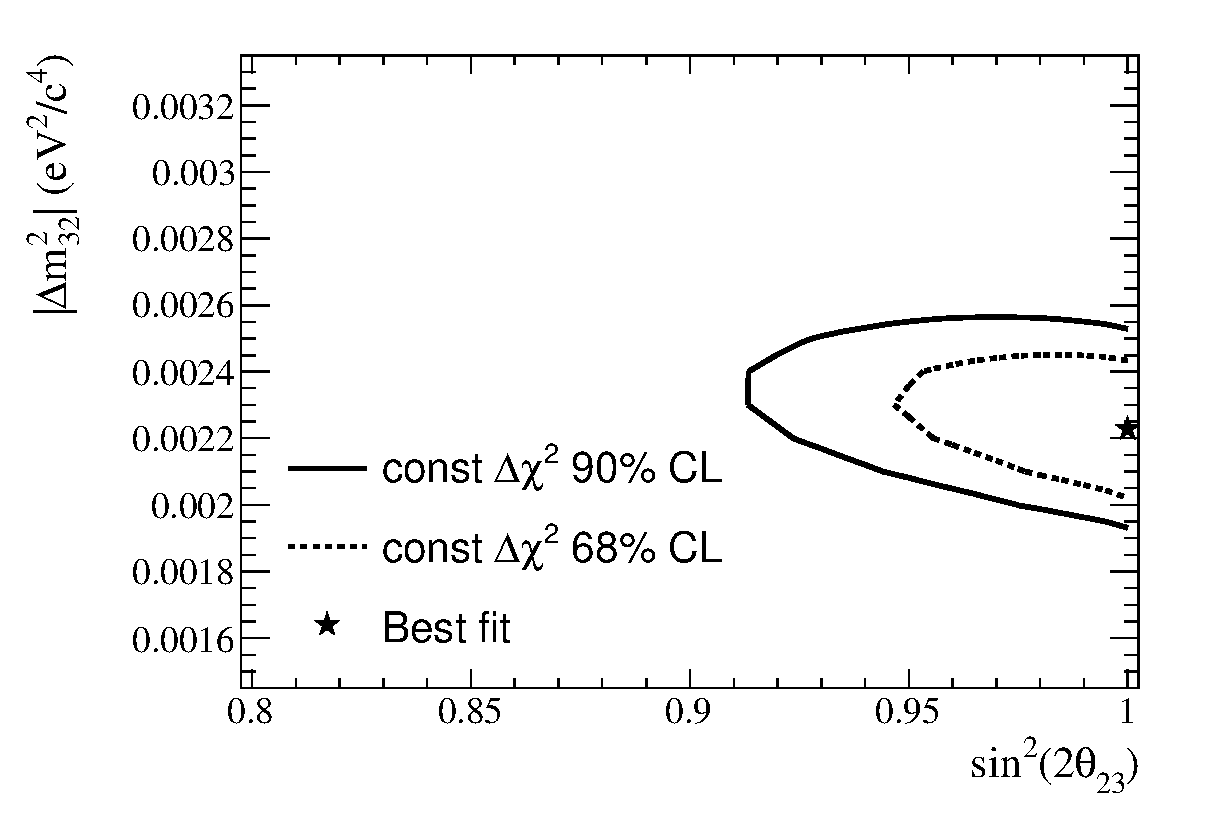
\includegraphics[width=18pc]{./images/fit_toymc/example_fits/2N/contours_3}
\caption { 
  68\% and 90\% confidence regions for the 2+N fit to fake data set 3
}
\label{fig:fakedata_contours_2N_3}
\end{minipage}
\vfill
\begin{minipage}[t]{0.48\linewidth}
\center
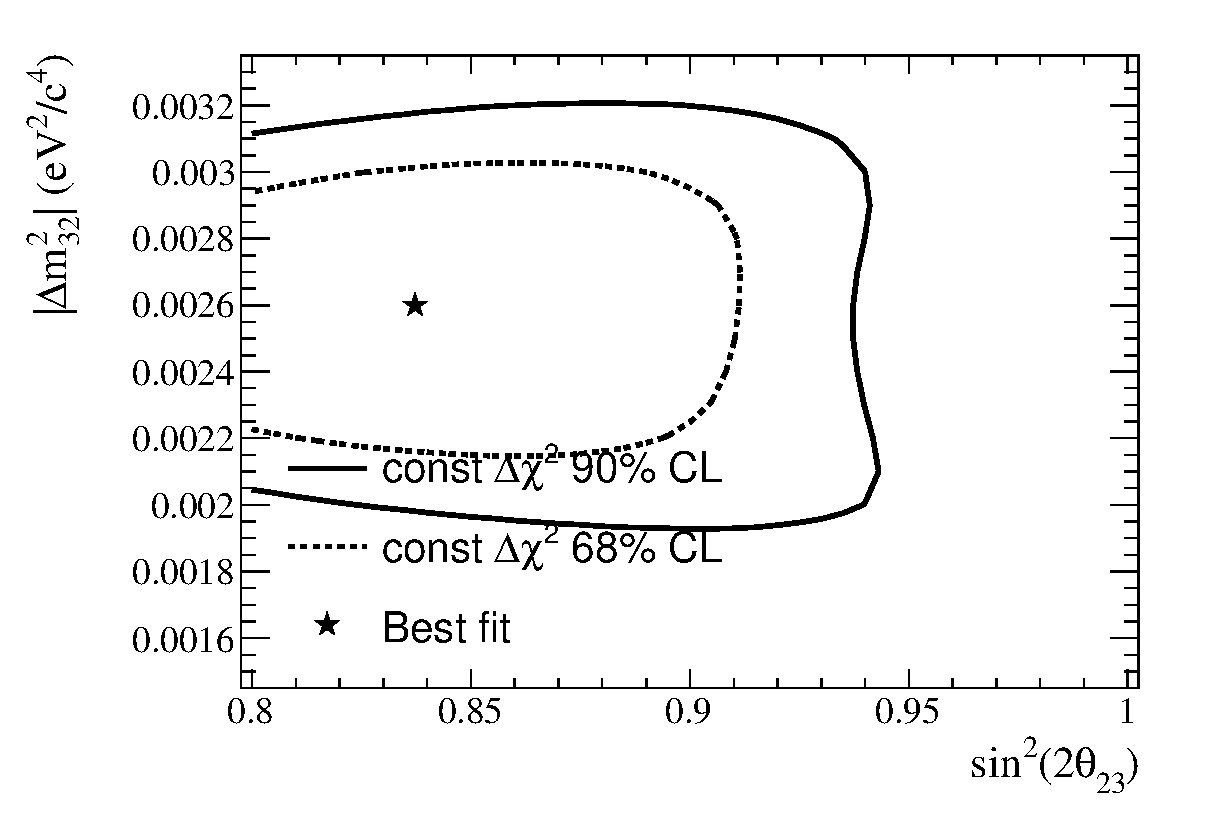
\includegraphics[width=18pc]{./images/fit_toymc/example_fits/2N/contours_4}
\caption {
  68\% and 90\% confidence regions for the 2+N fit to fake data set 4
}
\label{fig:fakedata_contours_2N_4}
\end{minipage}
\hspace{0.06\linewidth}
\begin{minipage}[t]{0.48\linewidth}
\center
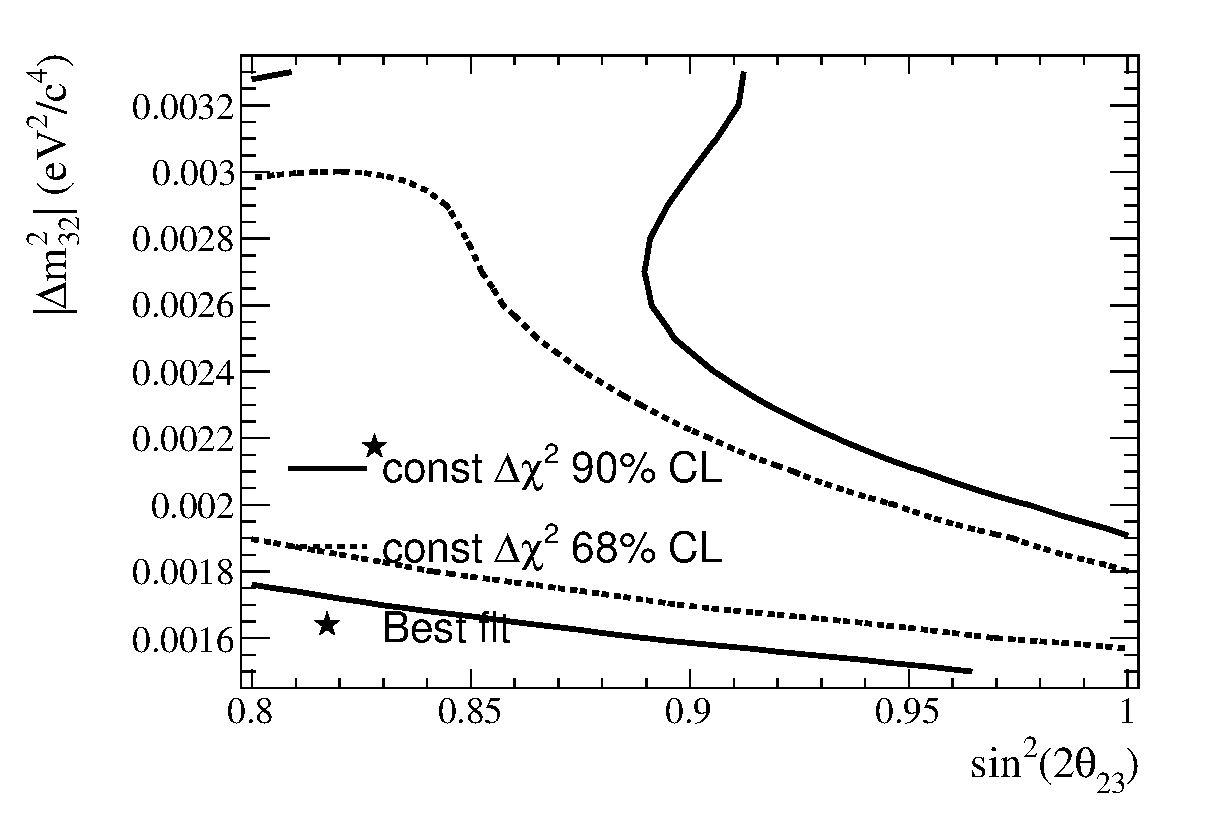
\includegraphics[width=18pc]{./images/fit_toymc/example_fits/2N/contours_5}
\caption { 
  68\% and 90\% confidence regions for the 2+N fit to fake data set 5
}
\label{fig:fakedata_contours_2N_5}
\end{minipage}
\end{figure*}


%...........................................................
%
% Contours for `2+8' fits
%

\begin{figure*}[htb]
\begin{minipage}[t]{0.48\linewidth}
\center
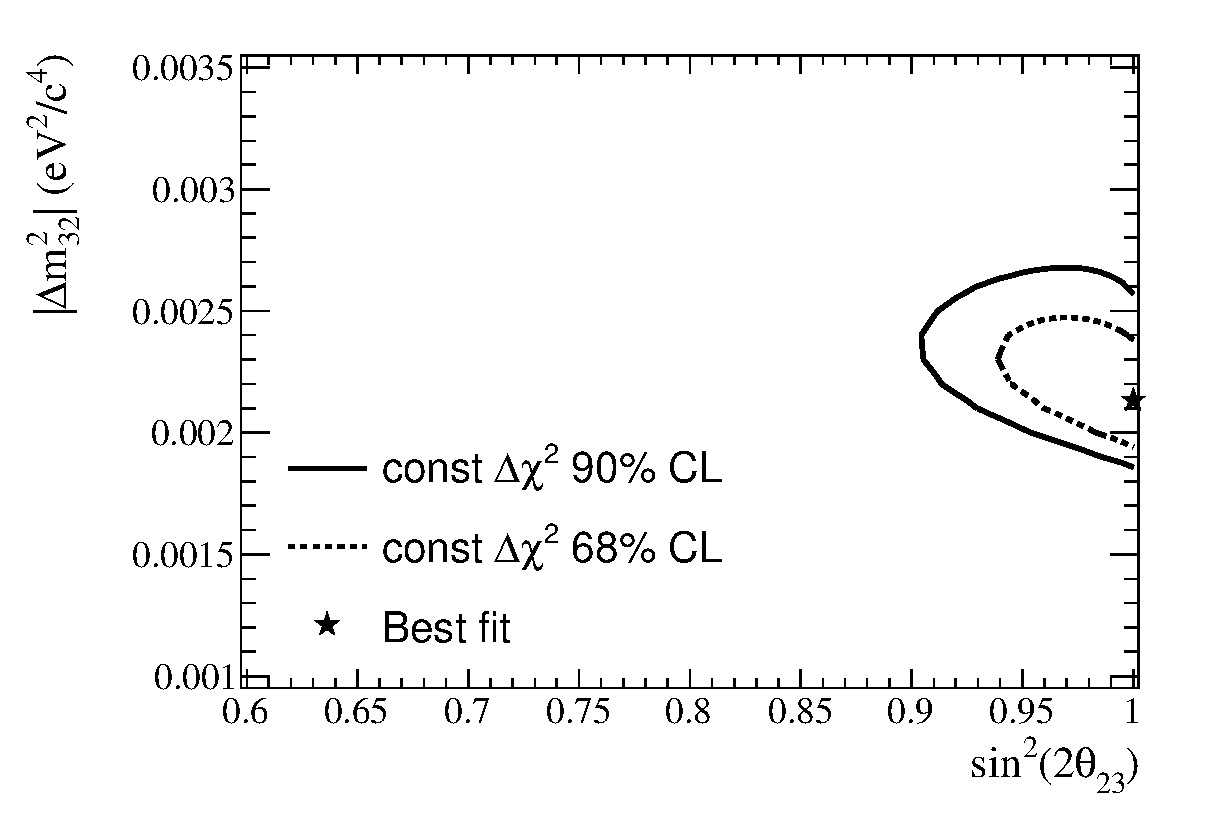
\includegraphics[width=18pc]{./images/fit_toymc/example_fits/contours_0}
\caption {
  68\% and 90\% confidence regions for the 2+8 fit to fake data set 0
}
\label{fig:fakedata_contours_0}
\end{minipage}
\hspace{0.06\linewidth}
\begin{minipage}[t]{0.48\linewidth}
\center
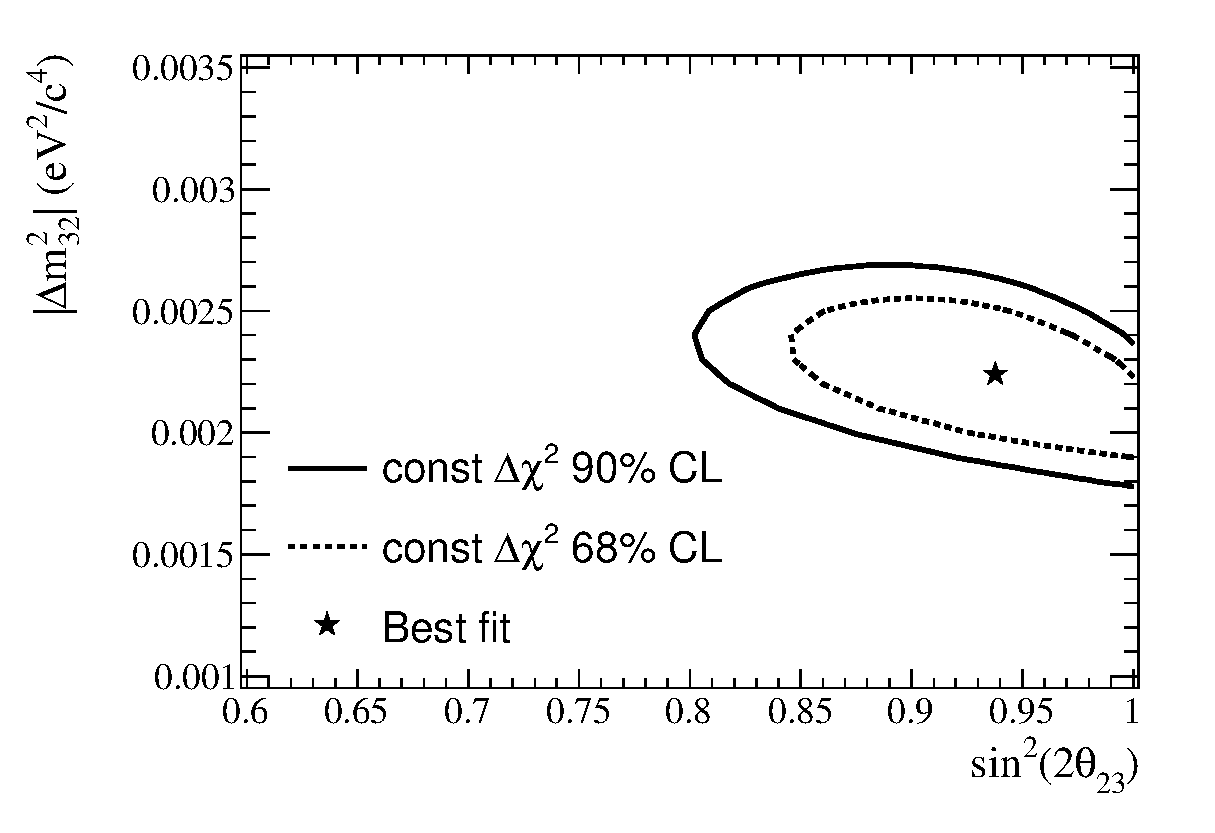
\includegraphics[width=18pc]{./images/fit_toymc/example_fits/contours_1}
\caption { 
  68\% and 90\% confidence regions for the 2+8 fit to fake data set 1
}
\label{fig:fakedata_contours_1}
\end{minipage}
\vfill
\begin{minipage}[t]{0.48\linewidth}
\center
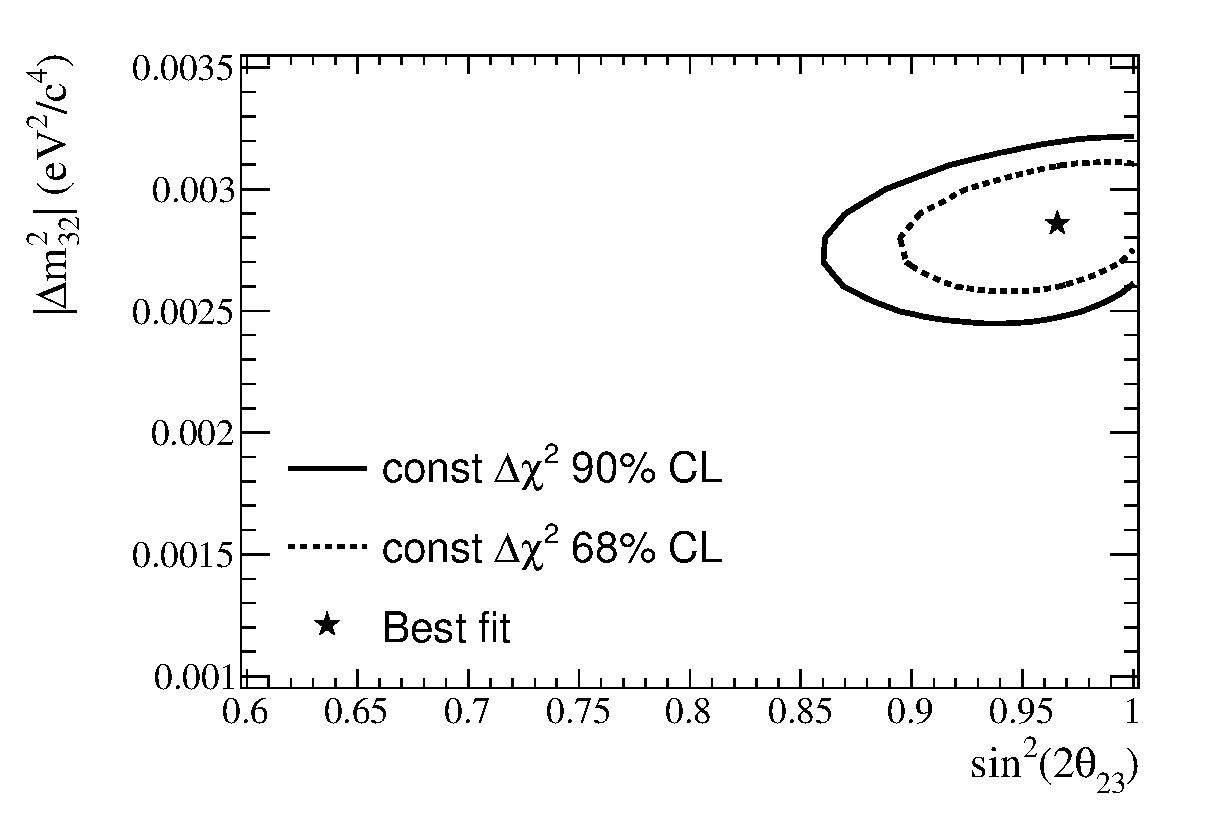
\includegraphics[width=18pc]{./images/fit_toymc/example_fits/contours_2}
\caption {
  68\% and 90\% confidence regions for the 2+8 fit to fake data set 2
}
\label{fig:fakedata_contours_2}
\end{minipage}
\hspace{0.06\linewidth}
\begin{minipage}[t]{0.48\linewidth}
\center
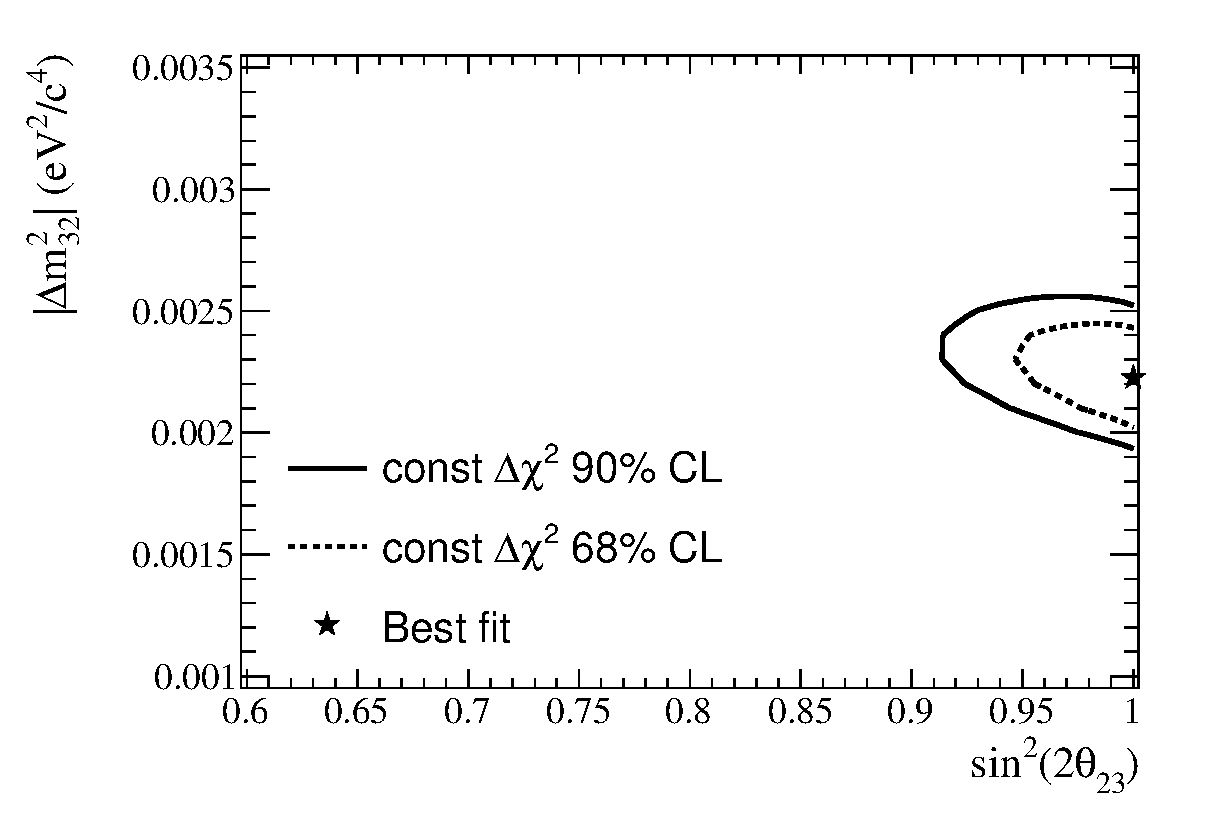
\includegraphics[width=18pc]{./images/fit_toymc/example_fits/contours_3}
\caption { 
  68\% and 90\% confidence regions for the 2+8 fit to fake data set 3
}
\label{fig:fakedata_contours_3}
\end{minipage}
\vfill
\begin{minipage}[t]{0.48\linewidth}
\center
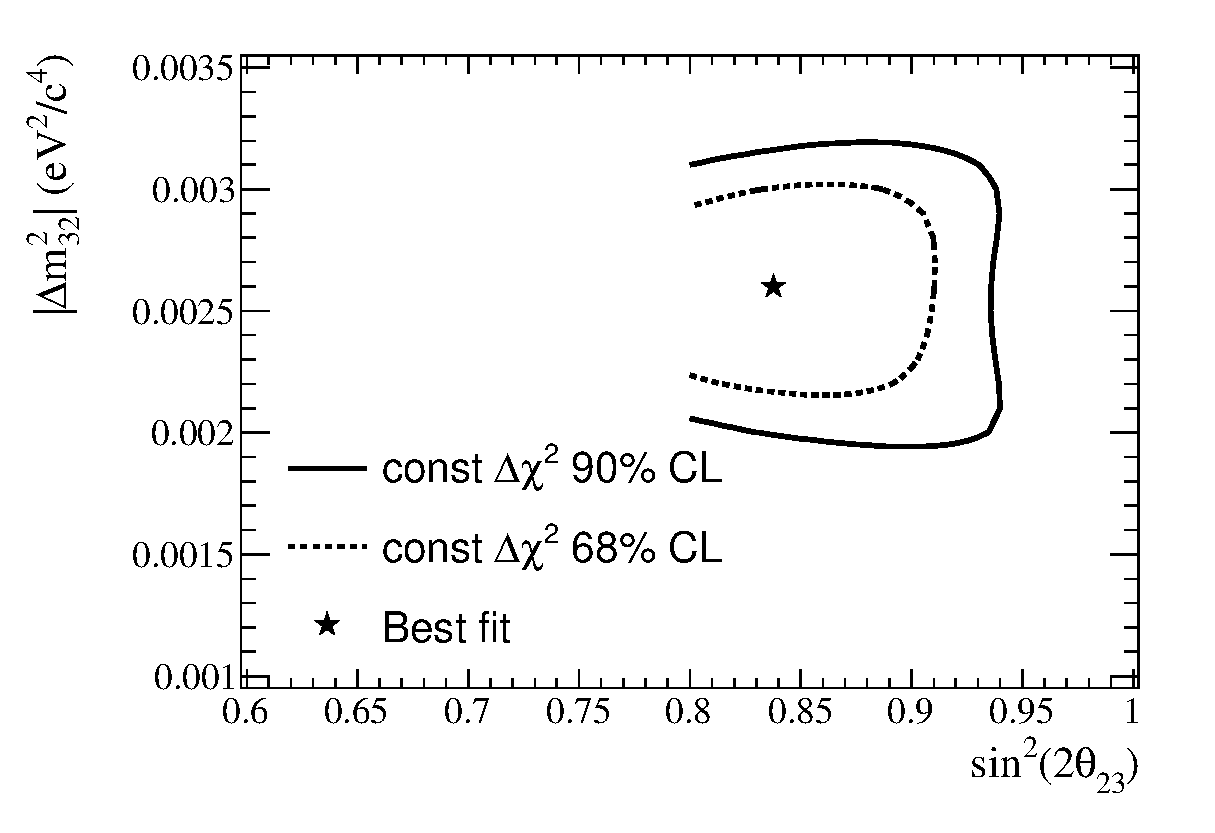
\includegraphics[width=18pc]{./images/fit_toymc/example_fits/contours_4}
\caption {
  68\% and 90\% confidence regions for the 2+8 fit to fake data set 4
}
\label{fig:fakedata_contours_4}
\end{minipage}
\hspace{0.06\linewidth}
\begin{minipage}[t]{0.48\linewidth}
\center
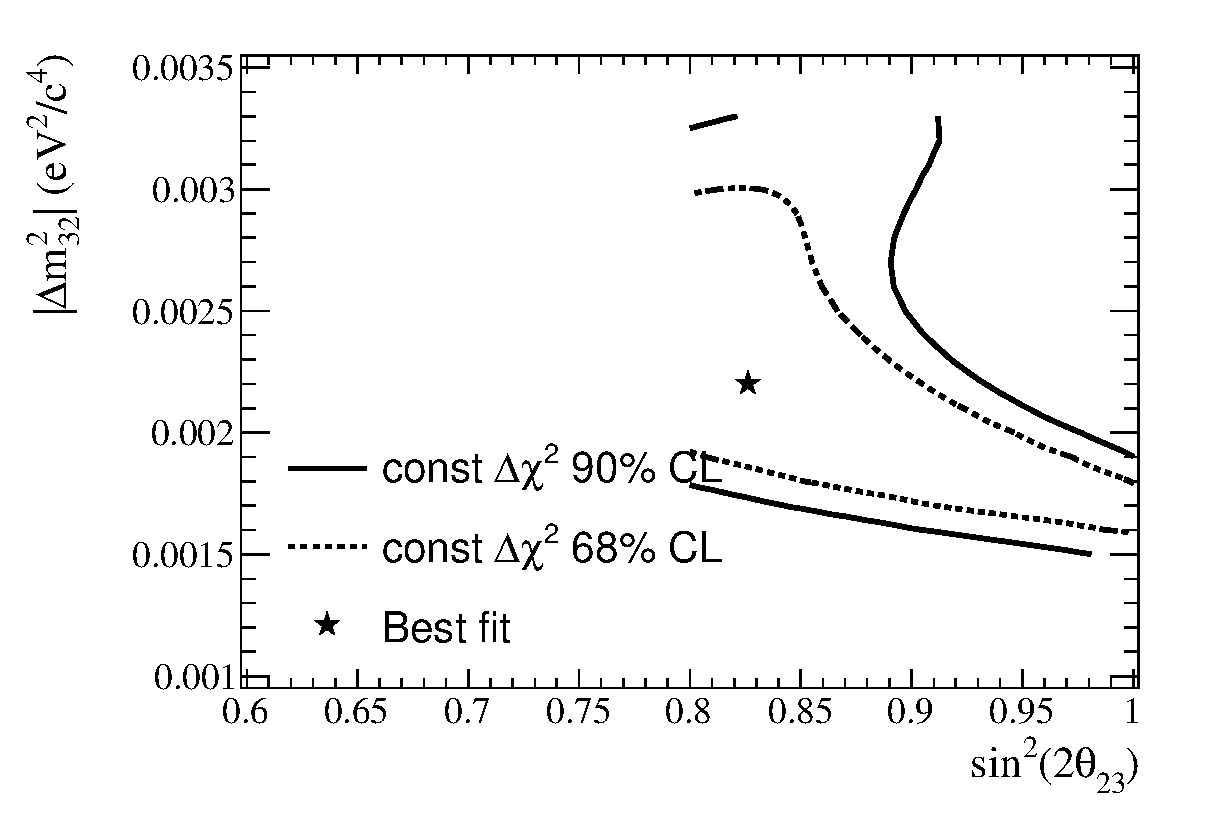
\includegraphics[width=18pc]{./images/fit_toymc/example_fits/contours_5}
\caption { 
  68\% and 90\% confidence regions for the 2+8 fit to fake data set 5
}
\label{fig:fakedata_contours_5}
\end{minipage}
\end{figure*}

\clearpage

\section{Detailed study of the effect of systematics on the predicted number of 1 $\mu$-like ring events}
\label{appendix:nsk_systematics}

In this section, the effect of systematics on the predicted number of events in SuperK is presented in a number of tables. 
Each table shows the pre- and post-BANFF tuning nominal $N_{SK}$ for every SuperK MC mode considered in the analysis, and 
the BANFF-tuned $N_{SK}$ for $\pm$1$\sigma$ deviations of a single systematic parameter. For correlated systematic parameters, 
$\sigma$ is defined as the square root of the corresponding diagonal entry in the covariance matrix.
For certain systematics, the modes are broken into $E_{reco}$ or $E_{true}$ bins, to show the energy dependence of that systematic 
(where relevant).
Tabs.\ \ref{tab:num_sk_energy_scale_1RmuT_3f_osc_t13:0_spectralreco_spectraltrue}-\ref{tab:num_fsi_005_1RmuT_3f_osc_t13:0_spectralreco_spectraltrue} 
show the effect of systematics on the unoscillated $N_{SK}$.
Tabs.\ \ref{tab:num_sk_energy_scale_1RmuT_3f_osc_t13:0.098_spectralreco_spectraltrue}-\ref{tab:num_fsi_005_1RmuT_3f_osc_t13:0.098_spectralreco_spectraltrue} 
show the effect of systematics on the $N_{SK}$ with 3-flavour oscillations in matter, using the following values of the oscillation parameters:
\begin{itemize}
\item $\sin^22\theta_{12} = $ 0.857
\item $\sin^22\theta_{13} = $ 0.098
\item $\sin^22\theta_{23} = $ 1.0
\item $\delta_{CP} = $        0
\item $\Delta m^2_{21} = $    7.5$\times$10$^{-5}$ eV$^{2}$/c$^{4}$
\item $|\Delta m^2_{32}| = $  2.4$\times$10$^{-3}$ eV$^{2}$/c$^{4}$
\end{itemize}
The percentage uncertainties in the systematic parameters are summarised in Tab.\ \ref{tab:nsk_expectations} (parameters whose effects 
are evaluated using splines are not included in this table).


\begin{table}[b]
\scriptsize
\centering
\begin{tabular}{| l | r |}
\hline
                                                              {\bf Systematic}   & {\bf Expected change}  \\ 
\hline
                                                                 $f_{E; r}^{SK}$ &               0 \%  (movement in Ereco) \\ 
                                                           $f_{CCQEoth; r}^{SK}$ &             1.8 \%  \\ 
                                                           $f_{CCQERC0; r}^{SK}$ &             1.7 \%  \\ 
                                                           $f_{CCQERC1; r}^{SK}$ &             3.5 \%  \\ 
                                                           $f_{CCQERC2; r}^{SK}$ &             9.3 \%  \\ 
                                                             $f_{CCnQE; r}^{SK}$ &              20 \%  \\ 
                                                                $f_{NC; r}^{SK}$ &             111 \%  \\ 
                                                             $f_{\nu_e; r}^{SK}$ &             100 \%  \\ 
                                                           $f_{0; t, r}^{banff}$ &           9.283 \%  \\ 
                                                           $f_{1; t, r}^{banff}$ &           9.757 \%  \\ 
                                                           $f_{2; t, r}^{banff}$ &           8.974 \%  \\ 
                                                           $f_{3; t, r}^{banff}$ &           8.457 \%  \\ 
                                                           $f_{4; t, r}^{banff}$ &            10.5 \%  \\ 
                                                           $f_{5; t, r}^{banff}$ &            9.26 \%  \\ 
                                                           $f_{6; t, r}^{banff}$ &           8.113 \%  \\ 
                                                           $f_{7; t, r}^{banff}$ &           7.279 \%  \\ 
                                                           $f_{8; t, r}^{banff}$ &           8.362 \%  \\ 
                                                           $f_{9; t, r}^{banff}$ &           10.77 \%  \\ 
                                                          $f_{10; t, r}^{banff}$ &           14.12 \%  \\ 
                                                          $f_{11; t, r}^{banff}$ &           11.03 \%  \\ 
                                                          $f_{12; t, r}^{banff}$ &           9.867 \%  \\ 
                                                          $f_{13; t, r}^{banff}$ &           10.33 \%  \\ 
                                                          $f_{14; t, r}^{banff}$ &           11.08 \%  \\ 
                                                          $f_{15; t, r}^{banff}$ &           10.91 \%  \\ 
                                                          $f_{18; t, r}^{banff}$ &           9.012 \%  \\ 
                                                          $f_{19; t, r}^{banff}$ &           29.57 \%  \\ 
                                                          $f_{20; t, r}^{banff}$ &            16.7 \%  \\ 
                                                          $f_{21; t, r}^{banff}$ &            14.9 \%  \\ 
                                                          $f_{22; t, r}^{banff}$ &           27.74 \%  \\ 
                                                                  $f_{CCcoh; t}$ &             100 \%  \\ 
                                                             $f_{NC1\pi^\pm; t}$ &              30 \%  \\ 
                                                                  $f_{NCoth; t}$ &              30 \%  \\ 
                                                                $f_{CC\nu_e; t}$ &               3 \%  \\ 
                                                            $f_{CC\bar{\nu}; t}$ &              40 \%  \\ 
                                                            $f_{23; t, r}^{FSI}$ &         0.00363 \%  \\ 
\hline
\end{tabular}
\caption{Summary table showing the magnitude of errors in the systematic parameters. The numbers should be compared with the 
changes in $N_{SK}$ in the other tables in this appendix. Systematics with complicated energy dependence are treated with 
response functions, and are not shown.}
\label{tab:nsk_expectations}
\end{table}


\begin{table}
\scriptsize
\begin{tabular}{| l | r | r | r  r | r  r |}
\hline \hline
{\bf Component} &  {\bf Nominal}   &  {\bf BANFF tuned} &  \multicolumn {2}{c|} { {\bf BANFF tuned +1$\sigma$} } &  \multicolumn {2}{c|} { {\bf BANFF tuned -1$\sigma$} } \\
\hline
                                                    $N_{SK}$ (1 $\mu$-like ring) &           210.5 &           204.7 &           204.7 & -5.553e-14 \%  &           204.7 & -6.941e-14 \%  \\ 
\hline
\hline
                $N_{SK}$ (1 $\mu$-like ring): $\nu_\mu$ CCQE ($E_{r} <$ 0.4 GeV) &           7.784 &           7.518 &           7.518 &        0 \%  &           7.518 &        0 \%  \\ 
       $N_{SK}$ (1 $\mu$-like ring): $\nu_\mu$ CCQE (0.4 $\leq E_{r} <$ 1.1 GeV) &           136.8 &           128.3 &           128.3 &        0 \%  &           128.3 &        0 \%  \\ 
             $N_{SK}$ (1 $\mu$-like ring): $\nu_\mu$ CCQE ($E_{r} \geq$ 1.1 GeV) &           21.78 &            19.2 &            19.2 &        0 \%  &            19.2 &        0 \%  \\ 
\hline
                                    $N_{SK}$ (1 $\mu$-like ring): $\nu_\mu$ CCQE &           166.4 &             155 &             155 &        0 \%  &             155 &        0 \%  \\ 
                               $N_{SK}$ (1 $\mu$-like ring): $\nu_\mu$ CC 1$\pi$ &           28.88 &           34.95 &           34.95 &        0 \%  &           34.95 &        0 \%  \\ 
                             $N_{SK}$ (1 $\mu$-like ring): $\nu_\mu$ CC coherent &           1.006 &          0.9503 &          0.9503 &        0 \%  &          0.9503 &        0 \%  \\ 
              $N_{SK}$ (1 $\mu$-like ring): $\nu_\mu$ CC other ($\nu_\mu$ disap) &           4.315 &           4.199 &           4.199 &        0 \%  &           4.199 &        0 \%  \\ 
                                $N_{SK}$ (1 $\mu$-like ring): $\nu_{\mu}$ CC all &           200.6 &           195.1 &           195.1 &        0 \%  &           195.1 &        0 \%  \\ 
\hline
              $N_{SK}$ (1 $\mu$-like ring): $\nu_\mu$/$\nu_\tau$ NC 1$\pi^{+/-}$ &           1.697 &           1.625 &           1.625 &        0 \%  &           1.625 &        0 \%  \\ 
     $N_{SK}$ (1 $\mu$-like ring): $\nu_\mu$/$\nu_\tau$ NC other ($\nu_\mu$ app) &           1.522 &           1.466 &           1.466 &        0 \%  &           1.466 &        0 \%  \\ 
                                $N_{SK}$ (1 $\mu$-like ring): $\nu_{\mu}$ NC all &           3.218 &           3.092 &           3.092 &        0 \%  &           3.092 &        0 \%  \\ 
\hline
\hline
\hline
          $N_{SK}$ (1 $\mu$-like ring): $\bar{\nu_\mu}$ CCQE ($E_{r} <$ 0.4 GeV) &          0.1497 &          0.1414 &          0.1414 &        0 \%  &          0.1414 &        0 \%  \\ 
 $N_{SK}$ (1 $\mu$-like ring): $\bar{\nu_\mu}$ CCQE (0.4 $\leq E_{r} <$ 1.1 GeV) &           1.979 &           1.873 &           1.873 &        0 \%  &           1.873 &        0 \%  \\ 
       $N_{SK}$ (1 $\mu$-like ring): $\bar{\nu_\mu}$ CCQE ($E_{r} \geq$ 1.1 GeV) &           2.331 &           1.967 &           1.967 &        0 \%  &           1.967 &        0 \%  \\ 
\hline
                              $N_{SK}$ (1 $\mu$-like ring): $\bar{\nu_\mu}$ CCQE &            4.46 &           3.981 &           3.981 &        0 \%  &           3.981 &        0 \%  \\ 
                         $N_{SK}$ (1 $\mu$-like ring): $\bar{\nu_\mu}$ CC 1$\pi$ &           1.445 &           1.762 &           1.762 &        0 \%  &           1.762 &        0 \%  \\ 
                       $N_{SK}$ (1 $\mu$-like ring): $\bar{\nu_\mu}$ CC coherent &          0.2111 &          0.2028 &          0.2028 &        0 \%  &          0.2028 &        0 \%  \\ 
        $N_{SK}$ (1 $\mu$-like ring): $\bar{\nu_\mu}$ CC other ($\nu_\mu$ disap) &          0.2539 &          0.2478 &          0.2478 &        0 \%  &          0.2478 &        0 \%  \\ 
                          $N_{SK}$ (1 $\mu$-like ring): $\bar{\nu_{\mu}}$ CC all &            6.37 &           6.194 &           6.194 &        0 \%  &           6.194 &        0 \%  \\ 
\hline
  $N_{SK}$ (1 $\mu$-like ring): $\bar{\nu_\mu}$/$\bar{\nu_\tau}$ NC 1$\pi^{+/-}$ &         0.09198 &         0.09042 &         0.09042 &        0 \%  &         0.09042 &        0 \%  \\ 
$N_{SK}$ (1 $\mu$-like ring): $\bar{\nu_\mu}$/$\bar{\nu_\tau}$ NC other ($\nu_\mu$ app) &         0.07958 &         0.07761 &         0.07761 &        0 \%  &         0.07761 &        0 \%  \\ 
                          $N_{SK}$ (1 $\mu$-like ring): $\bar{\nu_{\mu}}$ NC all &          0.1716 &           0.168 &           0.168 &        0 \%  &           0.168 &        0 \%  \\ 
\hline
\hline
\hline
                                      $N_{SK}$ (1 $\mu$-like ring): $\nu_e$ CCQE &         0.01697 &         0.01626 &         0.01626 &        0 \%  &         0.01626 &        0 \%  \\ 
                                 $N_{SK}$ (1 $\mu$-like ring): $\nu_e$ CC 1$\pi$ &        0.009932 &         0.01313 &         0.01313 &        0 \%  &         0.01313 &        0 \%  \\ 
                               $N_{SK}$ (1 $\mu$-like ring): $\nu_e$ CC coherent &       0.0004335 &       0.0004335 &       0.0004335 &        0 \%  &       0.0004335 &        0 \%  \\ 
                $N_{SK}$ (1 $\mu$-like ring): $\nu_e$ CC other ($\nu_\mu$ disap) &        0.003048 &        0.003051 &        0.003051 &        0 \%  &        0.003051 &        0 \%  \\ 
                                  $N_{SK}$ (1 $\mu$-like ring): $\nu_{e}$ CC all &         0.03039 &         0.03287 &         0.03287 &        0 \%  &         0.03287 &        0 \%  \\ 
\hline
                           $N_{SK}$ (1 $\mu$-like ring): $\nu_e$ NC 1$\pi^{+/-}$ &         0.04865 &         0.04942 &         0.04942 &        0 \%  &         0.04942 &        0 \%  \\ 
                  $N_{SK}$ (1 $\mu$-like ring): $\nu_e$ NC other ($\nu_\mu$ app) &         0.05741 &         0.05768 &         0.05768 &        0 \%  &         0.05768 &        0 \%  \\ 
                                  $N_{SK}$ (1 $\mu$-like ring): $\nu_{e}$ NC all &          0.1061 &          0.1071 &          0.1071 &        0 \%  &          0.1071 &        0 \%  \\ 
\hline
\hline
\hline
                                $N_{SK}$ (1 $\mu$-like ring): $\bar{\nu_e}$ CCQE &        0.000827 &       0.0007905 &       0.0007905 &        0 \%  &       0.0007905 &        0 \%  \\ 
                           $N_{SK}$ (1 $\mu$-like ring): $\bar{\nu_e}$ CC 1$\pi$ &       0.0006013 &       0.0007453 &       0.0007453 &        0 \%  &       0.0007453 &        0 \%  \\ 
                         $N_{SK}$ (1 $\mu$-like ring): $\bar{\nu_e}$ CC coherent &       7.333e-05 &       7.333e-05 &       7.333e-05 &        0 \%  &       7.333e-05 &        0 \%  \\ 
          $N_{SK}$ (1 $\mu$-like ring): $\bar{\nu_e}$ CC other ($\nu_\mu$ disap) &       0.0002189 &        0.000219 &        0.000219 &        0 \%  &        0.000219 &        0 \%  \\ 
                            $N_{SK}$ (1 $\mu$-like ring): $\bar{\nu_{e}}$ CC all &        0.001721 &        0.001828 &        0.001828 &        0 \%  &        0.001828 &        0 \%  \\ 
\hline
                     $N_{SK}$ (1 $\mu$-like ring): $\bar{\nu_e}$ NC 1$\pi^{+/-}$ &        0.005805 &        0.005916 &        0.005916 &        0 \%  &        0.005916 &        0 \%  \\ 
            $N_{SK}$ (1 $\mu$-like ring): $\bar{\nu_e}$ NC other ($\nu_\mu$ app) &        0.005918 &        0.005954 &        0.005954 &        0 \%  &        0.005954 &        0 \%  \\ 
                            $N_{SK}$ (1 $\mu$-like ring): $\bar{\nu_{e}}$ NC all &         0.01172 &         0.01187 &         0.01187 &        0 \%  &         0.01187 &        0 \%  \\ 
\hline
\hline
\hline
                          $N_{SK}$ (1 $\mu$-like ring): oscillation $\nu_e$ CCQE &               0 &               0 &               0 &        0 \%  &               0 &        0 \%  \\ 
                     $N_{SK}$ (1 $\mu$-like ring): oscillation $\nu_e$ CC 1$\pi$ &               0 &               0 &               0 &        0 \%  &               0 &        0 \%  \\ 
                   $N_{SK}$ (1 $\mu$-like ring): oscillation $\nu_e$ CC coherent &               0 &               0 &               0 &        0 \%  &               0 &        0 \%  \\ 
      $N_{SK}$ (1 $\mu$-like ring): oscillation $\nu_e$ CC other ($\nu_\mu$ app) &               0 &               0 &               0 &        0 \%  &               0 &        0 \%  \\ 
                       $N_{SK}$ (1 $\mu$-like ring): oscillation $\nu_e$  CC all &               0 &               0 &               0 &        0 \%  &               0 &        0 \%  \\ 
\hline
\hline
\end{tabular}
\caption{ Effect of $f_{E; r}^{SK}$   for no oscillations (all mixing parameters set to 0).. }
\label{tab:num_sk_energy_scale_1RmuT_3f_osc_t13:0_spectralreco_spectraltrue}
\end{table}
\clearpage
\begin{table}
\scriptsize
\begin{tabular}{| l | r | r | r  r | r  r |}
\hline \hline
{\bf Component} &  {\bf Nominal}   &  {\bf BANFF tuned} &  \multicolumn {2}{c|} { {\bf BANFF tuned +1$\sigma$} } &  \multicolumn {2}{c|} { {\bf BANFF tuned -1$\sigma$} } \\
\hline
                                                    $N_{SK}$ (1 $\mu$-like ring) &           210.5 &           204.7 &           207.6 &    1.398 \%  &           201.9 &   -1.398 \%  \\ 
\hline
\hline
                                    $N_{SK}$ (1 $\mu$-like ring): $\nu_\mu$ CCQE &           166.4 &             155 &           157.8 &      1.8 \%  &           152.3 &     -1.8 \%  \\ 
                               $N_{SK}$ (1 $\mu$-like ring): $\nu_\mu$ CC 1$\pi$ &           28.88 &           34.95 &           34.95 &        0 \%  &           34.95 &        0 \%  \\ 
                             $N_{SK}$ (1 $\mu$-like ring): $\nu_\mu$ CC coherent &           1.006 &          0.9503 &          0.9503 &        0 \%  &          0.9503 &        0 \%  \\ 
              $N_{SK}$ (1 $\mu$-like ring): $\nu_\mu$ CC other ($\nu_\mu$ disap) &           4.315 &           4.199 &           4.199 &        0 \%  &           4.199 &        0 \%  \\ 
                                $N_{SK}$ (1 $\mu$-like ring): $\nu_{\mu}$ CC all &           200.6 &           195.1 &           197.9 &     1.43 \%  &           192.3 &    -1.43 \%  \\ 
\hline
              $N_{SK}$ (1 $\mu$-like ring): $\nu_\mu$/$\nu_\tau$ NC 1$\pi^{+/-}$ &           1.697 &           1.625 &           1.625 &        0 \%  &           1.625 &        0 \%  \\ 
     $N_{SK}$ (1 $\mu$-like ring): $\nu_\mu$/$\nu_\tau$ NC other ($\nu_\mu$ app) &           1.522 &           1.466 &           1.466 &        0 \%  &           1.466 &        0 \%  \\ 
                                $N_{SK}$ (1 $\mu$-like ring): $\nu_{\mu}$ NC all &           3.218 &           3.092 &           3.092 &        0 \%  &           3.092 &        0 \%  \\ 
\hline
\hline
\hline
                              $N_{SK}$ (1 $\mu$-like ring): $\bar{\nu_\mu}$ CCQE &            4.46 &           3.981 &           4.053 &      1.8 \%  &            3.91 &     -1.8 \%  \\ 
                         $N_{SK}$ (1 $\mu$-like ring): $\bar{\nu_\mu}$ CC 1$\pi$ &           1.445 &           1.762 &           1.762 &        0 \%  &           1.762 &        0 \%  \\ 
                       $N_{SK}$ (1 $\mu$-like ring): $\bar{\nu_\mu}$ CC coherent &          0.2111 &          0.2028 &          0.2028 &        0 \%  &          0.2028 &        0 \%  \\ 
        $N_{SK}$ (1 $\mu$-like ring): $\bar{\nu_\mu}$ CC other ($\nu_\mu$ disap) &          0.2539 &          0.2478 &          0.2478 &        0 \%  &          0.2478 &        0 \%  \\ 
                          $N_{SK}$ (1 $\mu$-like ring): $\bar{\nu_{\mu}}$ CC all &            6.37 &           6.194 &           6.266 &    1.157 \%  &           6.123 &   -1.157 \%  \\ 
\hline
  $N_{SK}$ (1 $\mu$-like ring): $\bar{\nu_\mu}$/$\bar{\nu_\tau}$ NC 1$\pi^{+/-}$ &         0.09198 &         0.09042 &         0.09042 &        0 \%  &         0.09042 &        0 \%  \\ 
$N_{SK}$ (1 $\mu$-like ring): $\bar{\nu_\mu}$/$\bar{\nu_\tau}$ NC other ($\nu_\mu$ app) &         0.07958 &         0.07761 &         0.07761 &        0 \%  &         0.07761 &        0 \%  \\ 
                          $N_{SK}$ (1 $\mu$-like ring): $\bar{\nu_{\mu}}$ NC all &          0.1716 &           0.168 &           0.168 &        0 \%  &           0.168 &        0 \%  \\ 
\hline
\hline
\hline
                                      $N_{SK}$ (1 $\mu$-like ring): $\nu_e$ CCQE &         0.01697 &         0.01626 &         0.01626 &        0 \%  &         0.01626 &        0 \%  \\ 
                                 $N_{SK}$ (1 $\mu$-like ring): $\nu_e$ CC 1$\pi$ &        0.009932 &         0.01313 &         0.01313 &        0 \%  &         0.01313 &        0 \%  \\ 
                               $N_{SK}$ (1 $\mu$-like ring): $\nu_e$ CC coherent &       0.0004335 &       0.0004335 &       0.0004335 &        0 \%  &       0.0004335 &        0 \%  \\ 
                $N_{SK}$ (1 $\mu$-like ring): $\nu_e$ CC other ($\nu_\mu$ disap) &        0.003048 &        0.003051 &        0.003051 &        0 \%  &        0.003051 &        0 \%  \\ 
                                  $N_{SK}$ (1 $\mu$-like ring): $\nu_{e}$ CC all &         0.03039 &         0.03287 &         0.03287 &        0 \%  &         0.03287 &        0 \%  \\ 
\hline
                           $N_{SK}$ (1 $\mu$-like ring): $\nu_e$ NC 1$\pi^{+/-}$ &         0.04865 &         0.04942 &         0.04942 &        0 \%  &         0.04942 &        0 \%  \\ 
                  $N_{SK}$ (1 $\mu$-like ring): $\nu_e$ NC other ($\nu_\mu$ app) &         0.05741 &         0.05768 &         0.05768 &        0 \%  &         0.05768 &        0 \%  \\ 
                                  $N_{SK}$ (1 $\mu$-like ring): $\nu_{e}$ NC all &          0.1061 &          0.1071 &          0.1071 &        0 \%  &          0.1071 &        0 \%  \\ 
\hline
\hline
\hline
                                $N_{SK}$ (1 $\mu$-like ring): $\bar{\nu_e}$ CCQE &        0.000827 &       0.0007905 &       0.0007905 &        0 \%  &       0.0007905 &        0 \%  \\ 
                           $N_{SK}$ (1 $\mu$-like ring): $\bar{\nu_e}$ CC 1$\pi$ &       0.0006013 &       0.0007453 &       0.0007453 &        0 \%  &       0.0007453 &        0 \%  \\ 
                         $N_{SK}$ (1 $\mu$-like ring): $\bar{\nu_e}$ CC coherent &       7.333e-05 &       7.333e-05 &       7.333e-05 &        0 \%  &       7.333e-05 &        0 \%  \\ 
          $N_{SK}$ (1 $\mu$-like ring): $\bar{\nu_e}$ CC other ($\nu_\mu$ disap) &       0.0002189 &        0.000219 &        0.000219 &        0 \%  &        0.000219 &        0 \%  \\ 
                            $N_{SK}$ (1 $\mu$-like ring): $\bar{\nu_{e}}$ CC all &        0.001721 &        0.001828 &        0.001828 &        0 \%  &        0.001828 &        0 \%  \\ 
\hline
                     $N_{SK}$ (1 $\mu$-like ring): $\bar{\nu_e}$ NC 1$\pi^{+/-}$ &        0.005805 &        0.005916 &        0.005916 &        0 \%  &        0.005916 &        0 \%  \\ 
            $N_{SK}$ (1 $\mu$-like ring): $\bar{\nu_e}$ NC other ($\nu_\mu$ app) &        0.005918 &        0.005954 &        0.005954 &        0 \%  &        0.005954 &        0 \%  \\ 
                            $N_{SK}$ (1 $\mu$-like ring): $\bar{\nu_{e}}$ NC all &         0.01172 &         0.01187 &         0.01187 &        0 \%  &         0.01187 &        0 \%  \\ 
\hline
\hline
\hline
                          $N_{SK}$ (1 $\mu$-like ring): oscillation $\nu_e$ CCQE &               0 &               0 &               0 &        0 \%  &               0 &        0 \%  \\ 
                     $N_{SK}$ (1 $\mu$-like ring): oscillation $\nu_e$ CC 1$\pi$ &               0 &               0 &               0 &        0 \%  &               0 &        0 \%  \\ 
                   $N_{SK}$ (1 $\mu$-like ring): oscillation $\nu_e$ CC coherent &               0 &               0 &               0 &        0 \%  &               0 &        0 \%  \\ 
      $N_{SK}$ (1 $\mu$-like ring): oscillation $\nu_e$ CC other ($\nu_\mu$ app) &               0 &               0 &               0 &        0 \%  &               0 &        0 \%  \\ 
                       $N_{SK}$ (1 $\mu$-like ring): oscillation $\nu_e$  CC all &               0 &               0 &               0 &        0 \%  &               0 &        0 \%  \\ 
\hline
\hline
\end{tabular}
\caption{ Effect of $f_{CCQEoth; r}^{SK}$ for no oscillations (all mixing parameters set to 0).. }
\label{tab:num_sk_1Rmu_ccqe_other_eff_1RmuT_3f_osc_t13:0}
\end{table}
\clearpage
\begin{table}
\scriptsize
\begin{tabular}{| l | r | r | r  r | r  r |}
\hline \hline
{\bf Component} &  {\bf Nominal}   &  {\bf BANFF tuned} &  \multicolumn {2}{c|} { {\bf BANFF tuned +1$\sigma$} } &  \multicolumn {2}{c|} { {\bf BANFF tuned -1$\sigma$} } \\
\hline
                                                    $N_{SK}$ (1 $\mu$-like ring) &           210.5 &           204.7 &           204.9 &   0.0636 \%  &           204.6 &  -0.0636 \%  \\ 
\hline
\hline
                $N_{SK}$ (1 $\mu$-like ring): $\nu_\mu$ CCQE ($E_{r} <$ 0.4 GeV) &           7.784 &           7.518 &           7.646 &      1.7 \%  &            7.39 &     -1.7 \%  \\ 
       $N_{SK}$ (1 $\mu$-like ring): $\nu_\mu$ CCQE (0.4 $\leq E_{r} <$ 1.1 GeV) &           136.8 &           128.3 &           128.3 &        0 \%  &           128.3 &        0 \%  \\ 
             $N_{SK}$ (1 $\mu$-like ring): $\nu_\mu$ CCQE ($E_{r} \geq$ 1.1 GeV) &           21.78 &            19.2 &            19.2 &        0 \%  &            19.2 &        0 \%  \\ 
\hline
                                    $N_{SK}$ (1 $\mu$-like ring): $\nu_\mu$ CCQE &           166.4 &             155 &           155.2 &  0.08243 \%  &           154.9 & -0.08243 \%  \\ 
                               $N_{SK}$ (1 $\mu$-like ring): $\nu_\mu$ CC 1$\pi$ &           28.88 &           34.95 &           34.95 &        0 \%  &           34.95 &        0 \%  \\ 
                             $N_{SK}$ (1 $\mu$-like ring): $\nu_\mu$ CC coherent &           1.006 &          0.9503 &          0.9503 &        0 \%  &          0.9503 &        0 \%  \\ 
              $N_{SK}$ (1 $\mu$-like ring): $\nu_\mu$ CC other ($\nu_\mu$ disap) &           4.315 &           4.199 &           4.199 &        0 \%  &           4.199 &        0 \%  \\ 
                                $N_{SK}$ (1 $\mu$-like ring): $\nu_{\mu}$ CC all &           200.6 &           195.1 &           195.3 &  0.06549 \%  &             195 & -0.06549 \%  \\ 
\hline
              $N_{SK}$ (1 $\mu$-like ring): $\nu_\mu$/$\nu_\tau$ NC 1$\pi^{+/-}$ &           1.697 &           1.625 &           1.625 &        0 \%  &           1.625 &        0 \%  \\ 
     $N_{SK}$ (1 $\mu$-like ring): $\nu_\mu$/$\nu_\tau$ NC other ($\nu_\mu$ app) &           1.522 &           1.466 &           1.466 &        0 \%  &           1.466 &        0 \%  \\ 
                                $N_{SK}$ (1 $\mu$-like ring): $\nu_{\mu}$ NC all &           3.218 &           3.092 &           3.092 &        0 \%  &           3.092 &        0 \%  \\ 
\hline
\hline
\hline
          $N_{SK}$ (1 $\mu$-like ring): $\bar{\nu_\mu}$ CCQE ($E_{r} <$ 0.4 GeV) &          0.1497 &          0.1414 &          0.1438 &      1.7 \%  &           0.139 &     -1.7 \%  \\ 
 $N_{SK}$ (1 $\mu$-like ring): $\bar{\nu_\mu}$ CCQE (0.4 $\leq E_{r} <$ 1.1 GeV) &           1.979 &           1.873 &           1.873 &        0 \%  &           1.873 &        0 \%  \\ 
       $N_{SK}$ (1 $\mu$-like ring): $\bar{\nu_\mu}$ CCQE ($E_{r} \geq$ 1.1 GeV) &           2.331 &           1.967 &           1.967 &        0 \%  &           1.967 &        0 \%  \\ 
\hline
                              $N_{SK}$ (1 $\mu$-like ring): $\bar{\nu_\mu}$ CCQE &            4.46 &           3.981 &           3.984 &  0.06039 \%  &           3.979 & -0.06039 \%  \\ 
                         $N_{SK}$ (1 $\mu$-like ring): $\bar{\nu_\mu}$ CC 1$\pi$ &           1.445 &           1.762 &           1.762 &        0 \%  &           1.762 &        0 \%  \\ 
                       $N_{SK}$ (1 $\mu$-like ring): $\bar{\nu_\mu}$ CC coherent &          0.2111 &          0.2028 &          0.2028 &        0 \%  &          0.2028 &        0 \%  \\ 
        $N_{SK}$ (1 $\mu$-like ring): $\bar{\nu_\mu}$ CC other ($\nu_\mu$ disap) &          0.2539 &          0.2478 &          0.2478 &        0 \%  &          0.2478 &        0 \%  \\ 
                          $N_{SK}$ (1 $\mu$-like ring): $\bar{\nu_{\mu}}$ CC all &            6.37 &           6.194 &           6.197 &  0.03881 \%  &           6.192 & -0.03881 \%  \\ 
\hline
  $N_{SK}$ (1 $\mu$-like ring): $\bar{\nu_\mu}$/$\bar{\nu_\tau}$ NC 1$\pi^{+/-}$ &         0.09198 &         0.09042 &         0.09042 &        0 \%  &         0.09042 &        0 \%  \\ 
$N_{SK}$ (1 $\mu$-like ring): $\bar{\nu_\mu}$/$\bar{\nu_\tau}$ NC other ($\nu_\mu$ app) &         0.07958 &         0.07761 &         0.07761 &        0 \%  &         0.07761 &        0 \%  \\ 
                          $N_{SK}$ (1 $\mu$-like ring): $\bar{\nu_{\mu}}$ NC all &          0.1716 &           0.168 &           0.168 &        0 \%  &           0.168 &        0 \%  \\ 
\hline
\hline
\hline
                                      $N_{SK}$ (1 $\mu$-like ring): $\nu_e$ CCQE &         0.01697 &         0.01626 &         0.01626 &        0 \%  &         0.01626 &        0 \%  \\ 
                                 $N_{SK}$ (1 $\mu$-like ring): $\nu_e$ CC 1$\pi$ &        0.009932 &         0.01313 &         0.01313 &        0 \%  &         0.01313 &        0 \%  \\ 
                               $N_{SK}$ (1 $\mu$-like ring): $\nu_e$ CC coherent &       0.0004335 &       0.0004335 &       0.0004335 &        0 \%  &       0.0004335 &        0 \%  \\ 
                $N_{SK}$ (1 $\mu$-like ring): $\nu_e$ CC other ($\nu_\mu$ disap) &        0.003048 &        0.003051 &        0.003051 &        0 \%  &        0.003051 &        0 \%  \\ 
                                  $N_{SK}$ (1 $\mu$-like ring): $\nu_{e}$ CC all &         0.03039 &         0.03287 &         0.03287 &        0 \%  &         0.03287 &        0 \%  \\ 
\hline
                           $N_{SK}$ (1 $\mu$-like ring): $\nu_e$ NC 1$\pi^{+/-}$ &         0.04865 &         0.04942 &         0.04942 &        0 \%  &         0.04942 &        0 \%  \\ 
                  $N_{SK}$ (1 $\mu$-like ring): $\nu_e$ NC other ($\nu_\mu$ app) &         0.05741 &         0.05768 &         0.05768 &        0 \%  &         0.05768 &        0 \%  \\ 
                                  $N_{SK}$ (1 $\mu$-like ring): $\nu_{e}$ NC all &          0.1061 &          0.1071 &          0.1071 &        0 \%  &          0.1071 &        0 \%  \\ 
\hline
\hline
\hline
                                $N_{SK}$ (1 $\mu$-like ring): $\bar{\nu_e}$ CCQE &        0.000827 &       0.0007905 &       0.0007905 &        0 \%  &       0.0007905 &        0 \%  \\ 
                           $N_{SK}$ (1 $\mu$-like ring): $\bar{\nu_e}$ CC 1$\pi$ &       0.0006013 &       0.0007453 &       0.0007453 &        0 \%  &       0.0007453 &        0 \%  \\ 
                         $N_{SK}$ (1 $\mu$-like ring): $\bar{\nu_e}$ CC coherent &       7.333e-05 &       7.333e-05 &       7.333e-05 &        0 \%  &       7.333e-05 &        0 \%  \\ 
          $N_{SK}$ (1 $\mu$-like ring): $\bar{\nu_e}$ CC other ($\nu_\mu$ disap) &       0.0002189 &        0.000219 &        0.000219 &        0 \%  &        0.000219 &        0 \%  \\ 
                            $N_{SK}$ (1 $\mu$-like ring): $\bar{\nu_{e}}$ CC all &        0.001721 &        0.001828 &        0.001828 &        0 \%  &        0.001828 &        0 \%  \\ 
\hline
                     $N_{SK}$ (1 $\mu$-like ring): $\bar{\nu_e}$ NC 1$\pi^{+/-}$ &        0.005805 &        0.005916 &        0.005916 &        0 \%  &        0.005916 &        0 \%  \\ 
            $N_{SK}$ (1 $\mu$-like ring): $\bar{\nu_e}$ NC other ($\nu_\mu$ app) &        0.005918 &        0.005954 &        0.005954 &        0 \%  &        0.005954 &        0 \%  \\ 
                            $N_{SK}$ (1 $\mu$-like ring): $\bar{\nu_{e}}$ NC all &         0.01172 &         0.01187 &         0.01187 &        0 \%  &         0.01187 &        0 \%  \\ 
\hline
\hline
\hline
                          $N_{SK}$ (1 $\mu$-like ring): oscillation $\nu_e$ CCQE &               0 &               0 &               0 &        0 \%  &               0 &        0 \%  \\ 
                     $N_{SK}$ (1 $\mu$-like ring): oscillation $\nu_e$ CC 1$\pi$ &               0 &               0 &               0 &        0 \%  &               0 &        0 \%  \\ 
                   $N_{SK}$ (1 $\mu$-like ring): oscillation $\nu_e$ CC coherent &               0 &               0 &               0 &        0 \%  &               0 &        0 \%  \\ 
      $N_{SK}$ (1 $\mu$-like ring): oscillation $\nu_e$ CC other ($\nu_\mu$ app) &               0 &               0 &               0 &        0 \%  &               0 &        0 \%  \\ 
                       $N_{SK}$ (1 $\mu$-like ring): oscillation $\nu_e$  CC all &               0 &               0 &               0 &        0 \%  &               0 &        0 \%  \\ 
\hline
\hline
\end{tabular}
\caption{ Effect of $f_{CCQERC0; r}^{SK}$ for no oscillations (all mixing parameters set to 0).. }
\label{tab:num_sk_1Rmu_ccqe_ring_counting_eff_0_1RmuT_3f_osc_t13:0_spectralreco_spectraltrue}
\end{table}
\clearpage
\begin{table}
\scriptsize
\begin{tabular}{| l | r | r | r  r | r  r |}
\hline \hline
{\bf Component} &  {\bf Nominal}   &  {\bf BANFF tuned} &  \multicolumn {2}{c|} { {\bf BANFF tuned +1$\sigma$} } &  \multicolumn {2}{c|} { {\bf BANFF tuned -1$\sigma$} } \\
\hline
                                                    $N_{SK}$ (1 $\mu$-like ring) &           210.5 &           204.7 &           209.3 &    2.226 \%  &           200.2 &   -2.226 \%  \\ 
\hline
\hline
                $N_{SK}$ (1 $\mu$-like ring): $\nu_\mu$ CCQE ($E_{r} <$ 0.4 GeV) &           7.784 &           7.518 &           7.518 &        0 \%  &           7.518 &        0 \%  \\ 
       $N_{SK}$ (1 $\mu$-like ring): $\nu_\mu$ CCQE (0.4 $\leq E_{r} <$ 1.1 GeV) &           136.8 &           128.3 &           132.8 &      3.5 \%  &           123.8 &     -3.5 \%  \\ 
             $N_{SK}$ (1 $\mu$-like ring): $\nu_\mu$ CCQE ($E_{r} \geq$ 1.1 GeV) &           21.78 &            19.2 &            19.2 &        0 \%  &            19.2 &        0 \%  \\ 
\hline
                                    $N_{SK}$ (1 $\mu$-like ring): $\nu_\mu$ CCQE &           166.4 &             155 &           159.5 &    2.897 \%  &           150.6 &   -2.897 \%  \\ 
                               $N_{SK}$ (1 $\mu$-like ring): $\nu_\mu$ CC 1$\pi$ &           28.88 &           34.95 &           34.95 &        0 \%  &           34.95 &        0 \%  \\ 
                             $N_{SK}$ (1 $\mu$-like ring): $\nu_\mu$ CC coherent &           1.006 &          0.9503 &          0.9503 &        0 \%  &          0.9503 &        0 \%  \\ 
              $N_{SK}$ (1 $\mu$-like ring): $\nu_\mu$ CC other ($\nu_\mu$ disap) &           4.315 &           4.199 &           4.199 &        0 \%  &           4.199 &        0 \%  \\ 
                                $N_{SK}$ (1 $\mu$-like ring): $\nu_{\mu}$ CC all &           200.6 &           195.1 &           199.6 &    2.302 \%  &           190.6 &   -2.302 \%  \\ 
\hline
              $N_{SK}$ (1 $\mu$-like ring): $\nu_\mu$/$\nu_\tau$ NC 1$\pi^{+/-}$ &           1.697 &           1.625 &           1.625 &        0 \%  &           1.625 &        0 \%  \\ 
     $N_{SK}$ (1 $\mu$-like ring): $\nu_\mu$/$\nu_\tau$ NC other ($\nu_\mu$ app) &           1.522 &           1.466 &           1.466 &        0 \%  &           1.466 &        0 \%  \\ 
                                $N_{SK}$ (1 $\mu$-like ring): $\nu_{\mu}$ NC all &           3.218 &           3.092 &           3.092 &        0 \%  &           3.092 &        0 \%  \\ 
\hline
\hline
\hline
          $N_{SK}$ (1 $\mu$-like ring): $\bar{\nu_\mu}$ CCQE ($E_{r} <$ 0.4 GeV) &          0.1497 &          0.1414 &          0.1414 &        0 \%  &          0.1414 &        0 \%  \\ 
 $N_{SK}$ (1 $\mu$-like ring): $\bar{\nu_\mu}$ CCQE (0.4 $\leq E_{r} <$ 1.1 GeV) &           1.979 &           1.873 &           1.939 &      3.5 \%  &           1.808 &     -3.5 \%  \\ 
       $N_{SK}$ (1 $\mu$-like ring): $\bar{\nu_\mu}$ CCQE ($E_{r} \geq$ 1.1 GeV) &           2.331 &           1.967 &           1.967 &        0 \%  &           1.967 &        0 \%  \\ 
\hline
                              $N_{SK}$ (1 $\mu$-like ring): $\bar{\nu_\mu}$ CCQE &            4.46 &           3.981 &           4.047 &    1.647 \%  &           3.916 &   -1.647 \%  \\ 
                         $N_{SK}$ (1 $\mu$-like ring): $\bar{\nu_\mu}$ CC 1$\pi$ &           1.445 &           1.762 &           1.762 &        0 \%  &           1.762 &        0 \%  \\ 
                       $N_{SK}$ (1 $\mu$-like ring): $\bar{\nu_\mu}$ CC coherent &          0.2111 &          0.2028 &          0.2028 &        0 \%  &          0.2028 &        0 \%  \\ 
        $N_{SK}$ (1 $\mu$-like ring): $\bar{\nu_\mu}$ CC other ($\nu_\mu$ disap) &          0.2539 &          0.2478 &          0.2478 &        0 \%  &          0.2478 &        0 \%  \\ 
                          $N_{SK}$ (1 $\mu$-like ring): $\bar{\nu_{\mu}}$ CC all &            6.37 &           6.194 &            6.26 &    1.058 \%  &           6.129 &   -1.058 \%  \\ 
\hline
  $N_{SK}$ (1 $\mu$-like ring): $\bar{\nu_\mu}$/$\bar{\nu_\tau}$ NC 1$\pi^{+/-}$ &         0.09198 &         0.09042 &         0.09042 &        0 \%  &         0.09042 &        0 \%  \\ 
$N_{SK}$ (1 $\mu$-like ring): $\bar{\nu_\mu}$/$\bar{\nu_\tau}$ NC other ($\nu_\mu$ app) &         0.07958 &         0.07761 &         0.07761 &        0 \%  &         0.07761 &        0 \%  \\ 
                          $N_{SK}$ (1 $\mu$-like ring): $\bar{\nu_{\mu}}$ NC all &          0.1716 &           0.168 &           0.168 &        0 \%  &           0.168 &        0 \%  \\ 
\hline
\hline
\hline
                                      $N_{SK}$ (1 $\mu$-like ring): $\nu_e$ CCQE &         0.01697 &         0.01626 &         0.01626 &        0 \%  &         0.01626 &        0 \%  \\ 
                                 $N_{SK}$ (1 $\mu$-like ring): $\nu_e$ CC 1$\pi$ &        0.009932 &         0.01313 &         0.01313 &        0 \%  &         0.01313 &        0 \%  \\ 
                               $N_{SK}$ (1 $\mu$-like ring): $\nu_e$ CC coherent &       0.0004335 &       0.0004335 &       0.0004335 &        0 \%  &       0.0004335 &        0 \%  \\ 
                $N_{SK}$ (1 $\mu$-like ring): $\nu_e$ CC other ($\nu_\mu$ disap) &        0.003048 &        0.003051 &        0.003051 &        0 \%  &        0.003051 &        0 \%  \\ 
                                  $N_{SK}$ (1 $\mu$-like ring): $\nu_{e}$ CC all &         0.03039 &         0.03287 &         0.03287 &        0 \%  &         0.03287 &        0 \%  \\ 
\hline
                           $N_{SK}$ (1 $\mu$-like ring): $\nu_e$ NC 1$\pi^{+/-}$ &         0.04865 &         0.04942 &         0.04942 &        0 \%  &         0.04942 &        0 \%  \\ 
                  $N_{SK}$ (1 $\mu$-like ring): $\nu_e$ NC other ($\nu_\mu$ app) &         0.05741 &         0.05768 &         0.05768 &        0 \%  &         0.05768 &        0 \%  \\ 
                                  $N_{SK}$ (1 $\mu$-like ring): $\nu_{e}$ NC all &          0.1061 &          0.1071 &          0.1071 &        0 \%  &          0.1071 &        0 \%  \\ 
\hline
\hline
\hline
                                $N_{SK}$ (1 $\mu$-like ring): $\bar{\nu_e}$ CCQE &        0.000827 &       0.0007905 &       0.0007905 &        0 \%  &       0.0007905 &        0 \%  \\ 
                           $N_{SK}$ (1 $\mu$-like ring): $\bar{\nu_e}$ CC 1$\pi$ &       0.0006013 &       0.0007453 &       0.0007453 &        0 \%  &       0.0007453 &        0 \%  \\ 
                         $N_{SK}$ (1 $\mu$-like ring): $\bar{\nu_e}$ CC coherent &       7.333e-05 &       7.333e-05 &       7.333e-05 &        0 \%  &       7.333e-05 &        0 \%  \\ 
          $N_{SK}$ (1 $\mu$-like ring): $\bar{\nu_e}$ CC other ($\nu_\mu$ disap) &       0.0002189 &        0.000219 &        0.000219 &        0 \%  &        0.000219 &        0 \%  \\ 
                            $N_{SK}$ (1 $\mu$-like ring): $\bar{\nu_{e}}$ CC all &        0.001721 &        0.001828 &        0.001828 &        0 \%  &        0.001828 &        0 \%  \\ 
\hline
                     $N_{SK}$ (1 $\mu$-like ring): $\bar{\nu_e}$ NC 1$\pi^{+/-}$ &        0.005805 &        0.005916 &        0.005916 &        0 \%  &        0.005916 &        0 \%  \\ 
            $N_{SK}$ (1 $\mu$-like ring): $\bar{\nu_e}$ NC other ($\nu_\mu$ app) &        0.005918 &        0.005954 &        0.005954 &        0 \%  &        0.005954 &        0 \%  \\ 
                            $N_{SK}$ (1 $\mu$-like ring): $\bar{\nu_{e}}$ NC all &         0.01172 &         0.01187 &         0.01187 &        0 \%  &         0.01187 &        0 \%  \\ 
\hline
\hline
\hline
                          $N_{SK}$ (1 $\mu$-like ring): oscillation $\nu_e$ CCQE &               0 &               0 &               0 &        0 \%  &               0 &        0 \%  \\ 
                     $N_{SK}$ (1 $\mu$-like ring): oscillation $\nu_e$ CC 1$\pi$ &               0 &               0 &               0 &        0 \%  &               0 &        0 \%  \\ 
                   $N_{SK}$ (1 $\mu$-like ring): oscillation $\nu_e$ CC coherent &               0 &               0 &               0 &        0 \%  &               0 &        0 \%  \\ 
      $N_{SK}$ (1 $\mu$-like ring): oscillation $\nu_e$ CC other ($\nu_\mu$ app) &               0 &               0 &               0 &        0 \%  &               0 &        0 \%  \\ 
                       $N_{SK}$ (1 $\mu$-like ring): oscillation $\nu_e$  CC all &               0 &               0 &               0 &        0 \%  &               0 &        0 \%  \\ 
\hline
\hline
\end{tabular}
\caption{ Effect of $f_{CCQERC1; r}^{SK}$ for no oscillations (all mixing parameters set to 0).. }
\label{tab:num_sk_1Rmu_ccqe_ring_counting_eff_1_1RmuT_3f_osc_t13:0_spectralreco_spectraltrue}
\end{table}
\clearpage
\begin{table}
\scriptsize
\begin{tabular}{| l | r | r | r  r | r  r |}
\hline \hline
{\bf Component} &  {\bf Nominal}   &  {\bf BANFF tuned} &  \multicolumn {2}{c|} { {\bf BANFF tuned +1$\sigma$} } &  \multicolumn {2}{c|} { {\bf BANFF tuned -1$\sigma$} } \\
\hline
                                                    $N_{SK}$ (1 $\mu$-like ring) &           210.5 &           204.7 &           206.7 &   0.9614 \%  &           202.8 &  -0.9614 \%  \\ 
\hline
\hline
                $N_{SK}$ (1 $\mu$-like ring): $\nu_\mu$ CCQE ($E_{r} <$ 0.4 GeV) &           7.784 &           7.518 &           7.518 &        0 \%  &           7.518 &        0 \%  \\ 
       $N_{SK}$ (1 $\mu$-like ring): $\nu_\mu$ CCQE (0.4 $\leq E_{r} <$ 1.1 GeV) &           136.8 &           128.3 &           128.3 &        0 \%  &           128.3 &        0 \%  \\ 
             $N_{SK}$ (1 $\mu$-like ring): $\nu_\mu$ CCQE ($E_{r} \geq$ 1.1 GeV) &           21.78 &            19.2 &           20.98 &      9.3 \%  &           17.41 &     -9.3 \%  \\ 
\hline
                                    $N_{SK}$ (1 $\mu$-like ring): $\nu_\mu$ CCQE &           166.4 &             155 &           156.8 &    1.152 \%  &           153.3 &   -1.152 \%  \\ 
                               $N_{SK}$ (1 $\mu$-like ring): $\nu_\mu$ CC 1$\pi$ &           28.88 &           34.95 &           34.95 &        0 \%  &           34.95 &        0 \%  \\ 
                             $N_{SK}$ (1 $\mu$-like ring): $\nu_\mu$ CC coherent &           1.006 &          0.9503 &          0.9503 &        0 \%  &          0.9503 &        0 \%  \\ 
              $N_{SK}$ (1 $\mu$-like ring): $\nu_\mu$ CC other ($\nu_\mu$ disap) &           4.315 &           4.199 &           4.199 &        0 \%  &           4.199 &        0 \%  \\ 
                                $N_{SK}$ (1 $\mu$-like ring): $\nu_{\mu}$ CC all &           200.6 &           195.1 &           196.9 &    0.915 \%  &           193.4 &   -0.915 \%  \\ 
\hline
              $N_{SK}$ (1 $\mu$-like ring): $\nu_\mu$/$\nu_\tau$ NC 1$\pi^{+/-}$ &           1.697 &           1.625 &           1.625 &        0 \%  &           1.625 &        0 \%  \\ 
     $N_{SK}$ (1 $\mu$-like ring): $\nu_\mu$/$\nu_\tau$ NC other ($\nu_\mu$ app) &           1.522 &           1.466 &           1.466 &        0 \%  &           1.466 &        0 \%  \\ 
                                $N_{SK}$ (1 $\mu$-like ring): $\nu_{\mu}$ NC all &           3.218 &           3.092 &           3.092 &        0 \%  &           3.092 &        0 \%  \\ 
\hline
\hline
\hline
          $N_{SK}$ (1 $\mu$-like ring): $\bar{\nu_\mu}$ CCQE ($E_{r} <$ 0.4 GeV) &          0.1497 &          0.1414 &          0.1414 &        0 \%  &          0.1414 &        0 \%  \\ 
 $N_{SK}$ (1 $\mu$-like ring): $\bar{\nu_\mu}$ CCQE (0.4 $\leq E_{r} <$ 1.1 GeV) &           1.979 &           1.873 &           1.873 &        0 \%  &           1.873 &        0 \%  \\ 
       $N_{SK}$ (1 $\mu$-like ring): $\bar{\nu_\mu}$ CCQE ($E_{r} \geq$ 1.1 GeV) &           2.331 &           1.967 &            2.15 &      9.3 \%  &           1.784 &     -9.3 \%  \\ 
\hline
                              $N_{SK}$ (1 $\mu$-like ring): $\bar{\nu_\mu}$ CCQE &            4.46 &           3.981 &           4.164 &    4.594 \%  &           3.799 &   -4.594 \%  \\ 
                         $N_{SK}$ (1 $\mu$-like ring): $\bar{\nu_\mu}$ CC 1$\pi$ &           1.445 &           1.762 &           1.762 &        0 \%  &           1.762 &        0 \%  \\ 
                       $N_{SK}$ (1 $\mu$-like ring): $\bar{\nu_\mu}$ CC coherent &          0.2111 &          0.2028 &          0.2028 &        0 \%  &          0.2028 &        0 \%  \\ 
        $N_{SK}$ (1 $\mu$-like ring): $\bar{\nu_\mu}$ CC other ($\nu_\mu$ disap) &          0.2539 &          0.2478 &          0.2478 &        0 \%  &          0.2478 &        0 \%  \\ 
                          $N_{SK}$ (1 $\mu$-like ring): $\bar{\nu_{\mu}}$ CC all &            6.37 &           6.194 &           6.377 &    2.953 \%  &           6.012 &   -2.953 \%  \\ 
\hline
  $N_{SK}$ (1 $\mu$-like ring): $\bar{\nu_\mu}$/$\bar{\nu_\tau}$ NC 1$\pi^{+/-}$ &         0.09198 &         0.09042 &         0.09042 &        0 \%  &         0.09042 &        0 \%  \\ 
$N_{SK}$ (1 $\mu$-like ring): $\bar{\nu_\mu}$/$\bar{\nu_\tau}$ NC other ($\nu_\mu$ app) &         0.07958 &         0.07761 &         0.07761 &        0 \%  &         0.07761 &        0 \%  \\ 
                          $N_{SK}$ (1 $\mu$-like ring): $\bar{\nu_{\mu}}$ NC all &          0.1716 &           0.168 &           0.168 &        0 \%  &           0.168 &        0 \%  \\ 
\hline
\hline
\hline
                                      $N_{SK}$ (1 $\mu$-like ring): $\nu_e$ CCQE &         0.01697 &         0.01626 &         0.01626 &        0 \%  &         0.01626 &        0 \%  \\ 
                                 $N_{SK}$ (1 $\mu$-like ring): $\nu_e$ CC 1$\pi$ &        0.009932 &         0.01313 &         0.01313 &        0 \%  &         0.01313 &        0 \%  \\ 
                               $N_{SK}$ (1 $\mu$-like ring): $\nu_e$ CC coherent &       0.0004335 &       0.0004335 &       0.0004335 &        0 \%  &       0.0004335 &        0 \%  \\ 
                $N_{SK}$ (1 $\mu$-like ring): $\nu_e$ CC other ($\nu_\mu$ disap) &        0.003048 &        0.003051 &        0.003051 &        0 \%  &        0.003051 &        0 \%  \\ 
                                  $N_{SK}$ (1 $\mu$-like ring): $\nu_{e}$ CC all &         0.03039 &         0.03287 &         0.03287 &        0 \%  &         0.03287 &        0 \%  \\ 
\hline
                           $N_{SK}$ (1 $\mu$-like ring): $\nu_e$ NC 1$\pi^{+/-}$ &         0.04865 &         0.04942 &         0.04942 &        0 \%  &         0.04942 &        0 \%  \\ 
                  $N_{SK}$ (1 $\mu$-like ring): $\nu_e$ NC other ($\nu_\mu$ app) &         0.05741 &         0.05768 &         0.05768 &        0 \%  &         0.05768 &        0 \%  \\ 
                                  $N_{SK}$ (1 $\mu$-like ring): $\nu_{e}$ NC all &          0.1061 &          0.1071 &          0.1071 &        0 \%  &          0.1071 &        0 \%  \\ 
\hline
\hline
\hline
                                $N_{SK}$ (1 $\mu$-like ring): $\bar{\nu_e}$ CCQE &        0.000827 &       0.0007905 &       0.0007905 &        0 \%  &       0.0007905 &        0 \%  \\ 
                           $N_{SK}$ (1 $\mu$-like ring): $\bar{\nu_e}$ CC 1$\pi$ &       0.0006013 &       0.0007453 &       0.0007453 &        0 \%  &       0.0007453 &        0 \%  \\ 
                         $N_{SK}$ (1 $\mu$-like ring): $\bar{\nu_e}$ CC coherent &       7.333e-05 &       7.333e-05 &       7.333e-05 &        0 \%  &       7.333e-05 &        0 \%  \\ 
          $N_{SK}$ (1 $\mu$-like ring): $\bar{\nu_e}$ CC other ($\nu_\mu$ disap) &       0.0002189 &        0.000219 &        0.000219 &        0 \%  &        0.000219 &        0 \%  \\ 
                            $N_{SK}$ (1 $\mu$-like ring): $\bar{\nu_{e}}$ CC all &        0.001721 &        0.001828 &        0.001828 &        0 \%  &        0.001828 &        0 \%  \\ 
\hline
                     $N_{SK}$ (1 $\mu$-like ring): $\bar{\nu_e}$ NC 1$\pi^{+/-}$ &        0.005805 &        0.005916 &        0.005916 &        0 \%  &        0.005916 &        0 \%  \\ 
            $N_{SK}$ (1 $\mu$-like ring): $\bar{\nu_e}$ NC other ($\nu_\mu$ app) &        0.005918 &        0.005954 &        0.005954 &        0 \%  &        0.005954 &        0 \%  \\ 
                            $N_{SK}$ (1 $\mu$-like ring): $\bar{\nu_{e}}$ NC all &         0.01172 &         0.01187 &         0.01187 &        0 \%  &         0.01187 &        0 \%  \\ 
\hline
\hline
\hline
                          $N_{SK}$ (1 $\mu$-like ring): oscillation $\nu_e$ CCQE &               0 &               0 &               0 &        0 \%  &               0 &        0 \%  \\ 
                     $N_{SK}$ (1 $\mu$-like ring): oscillation $\nu_e$ CC 1$\pi$ &               0 &               0 &               0 &        0 \%  &               0 &        0 \%  \\ 
                   $N_{SK}$ (1 $\mu$-like ring): oscillation $\nu_e$ CC coherent &               0 &               0 &               0 &        0 \%  &               0 &        0 \%  \\ 
      $N_{SK}$ (1 $\mu$-like ring): oscillation $\nu_e$ CC other ($\nu_\mu$ app) &               0 &               0 &               0 &        0 \%  &               0 &        0 \%  \\ 
                       $N_{SK}$ (1 $\mu$-like ring): oscillation $\nu_e$  CC all &               0 &               0 &               0 &        0 \%  &               0 &        0 \%  \\ 
\hline
\hline
\end{tabular}
\caption{ Effect of $f_{CCQERC2; r}^{SK}$ for no oscillations (all mixing parameters set to 0).. }
\label{tab:num_sk_1Rmu_ccqe_ring_counting_eff_2_1RmuT_3f_osc_t13:0_spectralreco_spectraltrue}
\end{table}
\clearpage
\begin{table}
\scriptsize
\begin{tabular}{| l | r | r | r  r | r  r |}
\hline \hline
{\bf Component} &  {\bf Nominal}   &  {\bf BANFF tuned} &  \multicolumn {2}{c|} { {\bf BANFF tuned +1$\sigma$} } &  \multicolumn {2}{c|} { {\bf BANFF tuned -1$\sigma$} } \\
\hline
                                                    $N_{SK}$ (1 $\mu$-like ring) &           210.5 &           204.7 &           213.2 &    4.133 \%  &           196.3 &   -4.133 \%  \\ 
\hline
\hline
                                    $N_{SK}$ (1 $\mu$-like ring): $\nu_\mu$ CCQE &           166.4 &             155 &             155 &        0 \%  &             155 &        0 \%  \\ 
                               $N_{SK}$ (1 $\mu$-like ring): $\nu_\mu$ CC 1$\pi$ &           28.88 &           34.95 &           41.93 &       20 \%  &           27.96 &      -20 \%  \\ 
                             $N_{SK}$ (1 $\mu$-like ring): $\nu_\mu$ CC coherent &           1.006 &          0.9503 &            1.14 &       20 \%  &          0.7602 &      -20 \%  \\ 
              $N_{SK}$ (1 $\mu$-like ring): $\nu_\mu$ CC other ($\nu_\mu$ disap) &           4.315 &           4.199 &           5.038 &       20 \%  &           3.359 &      -20 \%  \\ 
                                $N_{SK}$ (1 $\mu$-like ring): $\nu_{\mu}$ CC all &           200.6 &           195.1 &           203.2 &    4.109 \%  &           187.1 &   -4.109 \%  \\ 
\hline
              $N_{SK}$ (1 $\mu$-like ring): $\nu_\mu$/$\nu_\tau$ NC 1$\pi^{+/-}$ &           1.697 &           1.625 &           1.625 &        0 \%  &           1.625 &        0 \%  \\ 
     $N_{SK}$ (1 $\mu$-like ring): $\nu_\mu$/$\nu_\tau$ NC other ($\nu_\mu$ app) &           1.522 &           1.466 &           1.466 &        0 \%  &           1.466 &        0 \%  \\ 
                                $N_{SK}$ (1 $\mu$-like ring): $\nu_{\mu}$ NC all &           3.218 &           3.092 &           3.092 &        0 \%  &           3.092 &        0 \%  \\ 
\hline
\hline
\hline
                              $N_{SK}$ (1 $\mu$-like ring): $\bar{\nu_\mu}$ CCQE &            4.46 &           3.981 &           3.981 &        0 \%  &           3.981 &        0 \%  \\ 
                         $N_{SK}$ (1 $\mu$-like ring): $\bar{\nu_\mu}$ CC 1$\pi$ &           1.445 &           1.762 &           2.115 &       20 \%  &            1.41 &      -20 \%  \\ 
                       $N_{SK}$ (1 $\mu$-like ring): $\bar{\nu_\mu}$ CC coherent &          0.2111 &          0.2028 &          0.2434 &       20 \%  &          0.1622 &      -20 \%  \\ 
        $N_{SK}$ (1 $\mu$-like ring): $\bar{\nu_\mu}$ CC other ($\nu_\mu$ disap) &          0.2539 &          0.2478 &          0.2974 &       20 \%  &          0.1982 &      -20 \%  \\ 
                          $N_{SK}$ (1 $\mu$-like ring): $\bar{\nu_{\mu}}$ CC all &            6.37 &           6.194 &           6.637 &    7.145 \%  &           5.752 &   -7.145 \%  \\ 
\hline
  $N_{SK}$ (1 $\mu$-like ring): $\bar{\nu_\mu}$/$\bar{\nu_\tau}$ NC 1$\pi^{+/-}$ &         0.09198 &         0.09042 &         0.09042 &        0 \%  &         0.09042 &        0 \%  \\ 
$N_{SK}$ (1 $\mu$-like ring): $\bar{\nu_\mu}$/$\bar{\nu_\tau}$ NC other ($\nu_\mu$ app) &         0.07958 &         0.07761 &         0.07761 &        0 \%  &         0.07761 &        0 \%  \\ 
                          $N_{SK}$ (1 $\mu$-like ring): $\bar{\nu_{\mu}}$ NC all &          0.1716 &           0.168 &           0.168 &        0 \%  &           0.168 &        0 \%  \\ 
\hline
\hline
\hline
                                      $N_{SK}$ (1 $\mu$-like ring): $\nu_e$ CCQE &         0.01697 &         0.01626 &         0.01626 &        0 \%  &         0.01626 &        0 \%  \\ 
                                 $N_{SK}$ (1 $\mu$-like ring): $\nu_e$ CC 1$\pi$ &        0.009932 &         0.01313 &         0.01313 &        0 \%  &         0.01313 &        0 \%  \\ 
                               $N_{SK}$ (1 $\mu$-like ring): $\nu_e$ CC coherent &       0.0004335 &       0.0004335 &       0.0004335 &        0 \%  &       0.0004335 &        0 \%  \\ 
                $N_{SK}$ (1 $\mu$-like ring): $\nu_e$ CC other ($\nu_\mu$ disap) &        0.003048 &        0.003051 &        0.003051 &        0 \%  &        0.003051 &        0 \%  \\ 
                                  $N_{SK}$ (1 $\mu$-like ring): $\nu_{e}$ CC all &         0.03039 &         0.03287 &         0.03287 &        0 \%  &         0.03287 &        0 \%  \\ 
\hline
                           $N_{SK}$ (1 $\mu$-like ring): $\nu_e$ NC 1$\pi^{+/-}$ &         0.04865 &         0.04942 &         0.04942 &        0 \%  &         0.04942 &        0 \%  \\ 
                  $N_{SK}$ (1 $\mu$-like ring): $\nu_e$ NC other ($\nu_\mu$ app) &         0.05741 &         0.05768 &         0.05768 &        0 \%  &         0.05768 &        0 \%  \\ 
                                  $N_{SK}$ (1 $\mu$-like ring): $\nu_{e}$ NC all &          0.1061 &          0.1071 &          0.1071 &        0 \%  &          0.1071 &        0 \%  \\ 
\hline
\hline
\hline
                                $N_{SK}$ (1 $\mu$-like ring): $\bar{\nu_e}$ CCQE &        0.000827 &       0.0007905 &       0.0007905 &        0 \%  &       0.0007905 &        0 \%  \\ 
                           $N_{SK}$ (1 $\mu$-like ring): $\bar{\nu_e}$ CC 1$\pi$ &       0.0006013 &       0.0007453 &       0.0007453 &        0 \%  &       0.0007453 &        0 \%  \\ 
                         $N_{SK}$ (1 $\mu$-like ring): $\bar{\nu_e}$ CC coherent &       7.333e-05 &       7.333e-05 &       7.333e-05 &        0 \%  &       7.333e-05 &        0 \%  \\ 
          $N_{SK}$ (1 $\mu$-like ring): $\bar{\nu_e}$ CC other ($\nu_\mu$ disap) &       0.0002189 &        0.000219 &        0.000219 &        0 \%  &        0.000219 &        0 \%  \\ 
                            $N_{SK}$ (1 $\mu$-like ring): $\bar{\nu_{e}}$ CC all &        0.001721 &        0.001828 &        0.001828 &        0 \%  &        0.001828 &        0 \%  \\ 
\hline
                     $N_{SK}$ (1 $\mu$-like ring): $\bar{\nu_e}$ NC 1$\pi^{+/-}$ &        0.005805 &        0.005916 &        0.005916 &        0 \%  &        0.005916 &        0 \%  \\ 
            $N_{SK}$ (1 $\mu$-like ring): $\bar{\nu_e}$ NC other ($\nu_\mu$ app) &        0.005918 &        0.005954 &        0.005954 &        0 \%  &        0.005954 &        0 \%  \\ 
                            $N_{SK}$ (1 $\mu$-like ring): $\bar{\nu_{e}}$ NC all &         0.01172 &         0.01187 &         0.01187 &        0 \%  &         0.01187 &        0 \%  \\ 
\hline
\hline
\hline
                          $N_{SK}$ (1 $\mu$-like ring): oscillation $\nu_e$ CCQE &               0 &               0 &               0 &        0 \%  &               0 &        0 \%  \\ 
                     $N_{SK}$ (1 $\mu$-like ring): oscillation $\nu_e$ CC 1$\pi$ &               0 &               0 &               0 &        0 \%  &               0 &        0 \%  \\ 
                   $N_{SK}$ (1 $\mu$-like ring): oscillation $\nu_e$ CC coherent &               0 &               0 &               0 &        0 \%  &               0 &        0 \%  \\ 
      $N_{SK}$ (1 $\mu$-like ring): oscillation $\nu_e$ CC other ($\nu_\mu$ app) &               0 &               0 &               0 &        0 \%  &               0 &        0 \%  \\ 
                       $N_{SK}$ (1 $\mu$-like ring): oscillation $\nu_e$  CC all &               0 &               0 &               0 &        0 \%  &               0 &        0 \%  \\ 
\hline
\hline
\end{tabular}
\caption{ Effect of $f_{CCnQE; r}^{SK}$ for no oscillations (all mixing parameters set to 0).. }
\label{tab:num_sk_1Rmu_ccnonqe_eff_1RmuT_3f_osc_t13:0}
\end{table}
\clearpage
\begin{table}
\scriptsize
\begin{tabular}{| l | r | r | r  r | r  r |}
\hline \hline
{\bf Component} &  {\bf Nominal}   &  {\bf BANFF tuned} &  \multicolumn {2}{c|} { {\bf BANFF tuned +1$\sigma$} } &  \multicolumn {2}{c|} { {\bf BANFF tuned -1$\sigma$} } \\
\hline
                                                    $N_{SK}$ (1 $\mu$-like ring) &           210.5 &           204.7 &           208.5 &    1.832 \%  &             201 &   -1.832 \%  \\ 
\hline
\hline
                                    $N_{SK}$ (1 $\mu$-like ring): $\nu_\mu$ CCQE &           166.4 &             155 &             155 &        0 \%  &             155 &        0 \%  \\ 
                               $N_{SK}$ (1 $\mu$-like ring): $\nu_\mu$ CC 1$\pi$ &           28.88 &           34.95 &           34.95 &        0 \%  &           34.95 &        0 \%  \\ 
                             $N_{SK}$ (1 $\mu$-like ring): $\nu_\mu$ CC coherent &           1.006 &          0.9503 &          0.9503 &        0 \%  &          0.9503 &        0 \%  \\ 
              $N_{SK}$ (1 $\mu$-like ring): $\nu_\mu$ CC other ($\nu_\mu$ disap) &           4.315 &           4.199 &           4.199 &        0 \%  &           4.199 &        0 \%  \\ 
                                $N_{SK}$ (1 $\mu$-like ring): $\nu_{\mu}$ CC all &           200.6 &           195.1 &           195.1 &        0 \%  &           195.1 &        0 \%  \\ 
\hline
              $N_{SK}$ (1 $\mu$-like ring): $\nu_\mu$/$\nu_\tau$ NC 1$\pi^{+/-}$ &           1.697 &           1.625 &            3.43 &      111 \%  &         -0.1788 &     -111 \%  \\ 
     $N_{SK}$ (1 $\mu$-like ring): $\nu_\mu$/$\nu_\tau$ NC other ($\nu_\mu$ app) &           1.522 &           1.466 &           3.094 &      111 \%  &         -0.1613 &     -111 \%  \\ 
                                $N_{SK}$ (1 $\mu$-like ring): $\nu_{\mu}$ NC all &           3.218 &           3.092 &           6.524 &      111 \%  &         -0.3401 &     -111 \%  \\ 
\hline
\hline
\hline
                              $N_{SK}$ (1 $\mu$-like ring): $\bar{\nu_\mu}$ CCQE &            4.46 &           3.981 &           3.981 &        0 \%  &           3.981 &        0 \%  \\ 
                         $N_{SK}$ (1 $\mu$-like ring): $\bar{\nu_\mu}$ CC 1$\pi$ &           1.445 &           1.762 &           1.762 &        0 \%  &           1.762 &        0 \%  \\ 
                       $N_{SK}$ (1 $\mu$-like ring): $\bar{\nu_\mu}$ CC coherent &          0.2111 &          0.2028 &          0.2028 &        0 \%  &          0.2028 &        0 \%  \\ 
        $N_{SK}$ (1 $\mu$-like ring): $\bar{\nu_\mu}$ CC other ($\nu_\mu$ disap) &          0.2539 &          0.2478 &          0.2478 &        0 \%  &          0.2478 &        0 \%  \\ 
                          $N_{SK}$ (1 $\mu$-like ring): $\bar{\nu_{\mu}}$ CC all &            6.37 &           6.194 &           6.194 &        0 \%  &           6.194 &        0 \%  \\ 
\hline
  $N_{SK}$ (1 $\mu$-like ring): $\bar{\nu_\mu}$/$\bar{\nu_\tau}$ NC 1$\pi^{+/-}$ &         0.09198 &         0.09042 &          0.1908 &      111 \%  &       -0.009946 &     -111 \%  \\ 
$N_{SK}$ (1 $\mu$-like ring): $\bar{\nu_\mu}$/$\bar{\nu_\tau}$ NC other ($\nu_\mu$ app) &         0.07958 &         0.07761 &          0.1638 &      111 \%  &       -0.008538 &     -111 \%  \\ 
                          $N_{SK}$ (1 $\mu$-like ring): $\bar{\nu_{\mu}}$ NC all &          0.1716 &           0.168 &          0.3546 &      111 \%  &        -0.01848 &     -111 \%  \\ 
\hline
\hline
\hline
                                      $N_{SK}$ (1 $\mu$-like ring): $\nu_e$ CCQE &         0.01697 &         0.01626 &         0.01626 &        0 \%  &         0.01626 &        0 \%  \\ 
                                 $N_{SK}$ (1 $\mu$-like ring): $\nu_e$ CC 1$\pi$ &        0.009932 &         0.01313 &         0.01313 &        0 \%  &         0.01313 &        0 \%  \\ 
                               $N_{SK}$ (1 $\mu$-like ring): $\nu_e$ CC coherent &       0.0004335 &       0.0004335 &       0.0004335 &        0 \%  &       0.0004335 &        0 \%  \\ 
                $N_{SK}$ (1 $\mu$-like ring): $\nu_e$ CC other ($\nu_\mu$ disap) &        0.003048 &        0.003051 &        0.003051 &        0 \%  &        0.003051 &        0 \%  \\ 
                                  $N_{SK}$ (1 $\mu$-like ring): $\nu_{e}$ CC all &         0.03039 &         0.03287 &         0.03287 &        0 \%  &         0.03287 &        0 \%  \\ 
\hline
                           $N_{SK}$ (1 $\mu$-like ring): $\nu_e$ NC 1$\pi^{+/-}$ &         0.04865 &         0.04942 &          0.1043 &      111 \%  &       -0.005436 &     -111 \%  \\ 
                  $N_{SK}$ (1 $\mu$-like ring): $\nu_e$ NC other ($\nu_\mu$ app) &         0.05741 &         0.05768 &          0.1217 &      111 \%  &       -0.006345 &     -111 \%  \\ 
                                  $N_{SK}$ (1 $\mu$-like ring): $\nu_{e}$ NC all &          0.1061 &          0.1071 &           0.226 &      111 \%  &        -0.01178 &     -111 \%  \\ 
\hline
\hline
\hline
                                $N_{SK}$ (1 $\mu$-like ring): $\bar{\nu_e}$ CCQE &        0.000827 &       0.0007905 &       0.0007905 &        0 \%  &       0.0007905 &        0 \%  \\ 
                           $N_{SK}$ (1 $\mu$-like ring): $\bar{\nu_e}$ CC 1$\pi$ &       0.0006013 &       0.0007453 &       0.0007453 &        0 \%  &       0.0007453 &        0 \%  \\ 
                         $N_{SK}$ (1 $\mu$-like ring): $\bar{\nu_e}$ CC coherent &       7.333e-05 &       7.333e-05 &       7.333e-05 &        0 \%  &       7.333e-05 &        0 \%  \\ 
          $N_{SK}$ (1 $\mu$-like ring): $\bar{\nu_e}$ CC other ($\nu_\mu$ disap) &       0.0002189 &        0.000219 &        0.000219 &        0 \%  &        0.000219 &        0 \%  \\ 
                            $N_{SK}$ (1 $\mu$-like ring): $\bar{\nu_{e}}$ CC all &        0.001721 &        0.001828 &        0.001828 &        0 \%  &        0.001828 &        0 \%  \\ 
\hline
                     $N_{SK}$ (1 $\mu$-like ring): $\bar{\nu_e}$ NC 1$\pi^{+/-}$ &        0.005805 &        0.005916 &         0.01248 &      111 \%  &      -0.0006508 &     -111 \%  \\ 
            $N_{SK}$ (1 $\mu$-like ring): $\bar{\nu_e}$ NC other ($\nu_\mu$ app) &        0.005918 &        0.005954 &         0.01256 &      111 \%  &      -0.0006549 &     -111 \%  \\ 
                            $N_{SK}$ (1 $\mu$-like ring): $\bar{\nu_{e}}$ NC all &         0.01172 &         0.01187 &         0.02505 &      111 \%  &       -0.001306 &     -111 \%  \\ 
\hline
\hline
\hline
                          $N_{SK}$ (1 $\mu$-like ring): oscillation $\nu_e$ CCQE &               0 &               0 &               0 &        0 \%  &               0 &        0 \%  \\ 
                     $N_{SK}$ (1 $\mu$-like ring): oscillation $\nu_e$ CC 1$\pi$ &               0 &               0 &               0 &        0 \%  &               0 &        0 \%  \\ 
                   $N_{SK}$ (1 $\mu$-like ring): oscillation $\nu_e$ CC coherent &               0 &               0 &               0 &        0 \%  &               0 &        0 \%  \\ 
      $N_{SK}$ (1 $\mu$-like ring): oscillation $\nu_e$ CC other ($\nu_\mu$ app) &               0 &               0 &               0 &        0 \%  &               0 &        0 \%  \\ 
                       $N_{SK}$ (1 $\mu$-like ring): oscillation $\nu_e$  CC all &               0 &               0 &               0 &        0 \%  &               0 &        0 \%  \\ 
\hline
\hline
\end{tabular}
\caption{ Effect of $f_{NC; r}^{SK}$ for no oscillations (all mixing parameters set to 0).. }
\label{tab:num_sk_1Rmu_nc_eff_1RmuT_3f_osc_t13:0}
\end{table}
\clearpage
\begin{table}
\scriptsize
\begin{tabular}{| l | r | r | r  r | r  r |}
\hline \hline
{\bf Component} &  {\bf Nominal}   &  {\bf BANFF tuned} &  \multicolumn {2}{c|} { {\bf BANFF tuned +1$\sigma$} } &  \multicolumn {2}{c|} { {\bf BANFF tuned -1$\sigma$} } \\
\hline
                                                    $N_{SK}$ (1 $\mu$-like ring) &           210.5 &           204.7 &           204.8 &  0.01695 \%  &           204.7 & -0.01695 \%  \\ 
\hline
\hline
                                    $N_{SK}$ (1 $\mu$-like ring): $\nu_\mu$ CCQE &           166.4 &             155 &             155 &        0 \%  &             155 &        0 \%  \\ 
                               $N_{SK}$ (1 $\mu$-like ring): $\nu_\mu$ CC 1$\pi$ &           28.88 &           34.95 &           34.95 &        0 \%  &           34.95 &        0 \%  \\ 
                             $N_{SK}$ (1 $\mu$-like ring): $\nu_\mu$ CC coherent &           1.006 &          0.9503 &          0.9503 &        0 \%  &          0.9503 &        0 \%  \\ 
              $N_{SK}$ (1 $\mu$-like ring): $\nu_\mu$ CC other ($\nu_\mu$ disap) &           4.315 &           4.199 &           4.199 &        0 \%  &           4.199 &        0 \%  \\ 
                                $N_{SK}$ (1 $\mu$-like ring): $\nu_{\mu}$ CC all &           200.6 &           195.1 &           195.1 &        0 \%  &           195.1 &        0 \%  \\ 
\hline
              $N_{SK}$ (1 $\mu$-like ring): $\nu_\mu$/$\nu_\tau$ NC 1$\pi^{+/-}$ &           1.697 &           1.625 &           1.625 &        0 \%  &           1.625 &        0 \%  \\ 
     $N_{SK}$ (1 $\mu$-like ring): $\nu_\mu$/$\nu_\tau$ NC other ($\nu_\mu$ app) &           1.522 &           1.466 &           1.466 &        0 \%  &           1.466 &        0 \%  \\ 
                                $N_{SK}$ (1 $\mu$-like ring): $\nu_{\mu}$ NC all &           3.218 &           3.092 &           3.092 &        0 \%  &           3.092 &        0 \%  \\ 
\hline
\hline
\hline
                              $N_{SK}$ (1 $\mu$-like ring): $\bar{\nu_\mu}$ CCQE &            4.46 &           3.981 &           3.981 &        0 \%  &           3.981 &        0 \%  \\ 
                         $N_{SK}$ (1 $\mu$-like ring): $\bar{\nu_\mu}$ CC 1$\pi$ &           1.445 &           1.762 &           1.762 &        0 \%  &           1.762 &        0 \%  \\ 
                       $N_{SK}$ (1 $\mu$-like ring): $\bar{\nu_\mu}$ CC coherent &          0.2111 &          0.2028 &          0.2028 &        0 \%  &          0.2028 &        0 \%  \\ 
        $N_{SK}$ (1 $\mu$-like ring): $\bar{\nu_\mu}$ CC other ($\nu_\mu$ disap) &          0.2539 &          0.2478 &          0.2478 &        0 \%  &          0.2478 &        0 \%  \\ 
                          $N_{SK}$ (1 $\mu$-like ring): $\bar{\nu_{\mu}}$ CC all &            6.37 &           6.194 &           6.194 &        0 \%  &           6.194 &        0 \%  \\ 
\hline
  $N_{SK}$ (1 $\mu$-like ring): $\bar{\nu_\mu}$/$\bar{\nu_\tau}$ NC 1$\pi^{+/-}$ &         0.09198 &         0.09042 &         0.09042 &        0 \%  &         0.09042 &        0 \%  \\ 
$N_{SK}$ (1 $\mu$-like ring): $\bar{\nu_\mu}$/$\bar{\nu_\tau}$ NC other ($\nu_\mu$ app) &         0.07958 &         0.07761 &         0.07761 &        0 \%  &         0.07761 &        0 \%  \\ 
                          $N_{SK}$ (1 $\mu$-like ring): $\bar{\nu_{\mu}}$ NC all &          0.1716 &           0.168 &           0.168 &        0 \%  &           0.168 &        0 \%  \\ 
\hline
\hline
\hline
                                      $N_{SK}$ (1 $\mu$-like ring): $\nu_e$ CCQE &         0.01697 &         0.01626 &         0.03252 &      100 \%  &               0 &     -100 \%  \\ 
                                 $N_{SK}$ (1 $\mu$-like ring): $\nu_e$ CC 1$\pi$ &        0.009932 &         0.01313 &         0.02625 &      100 \%  &               0 &     -100 \%  \\ 
                               $N_{SK}$ (1 $\mu$-like ring): $\nu_e$ CC coherent &       0.0004335 &       0.0004335 &        0.000867 &      100 \%  &               0 &     -100 \%  \\ 
                $N_{SK}$ (1 $\mu$-like ring): $\nu_e$ CC other ($\nu_\mu$ disap) &        0.003048 &        0.003051 &        0.006101 &      100 \%  &               0 &     -100 \%  \\ 
                                  $N_{SK}$ (1 $\mu$-like ring): $\nu_{e}$ CC all &         0.03039 &         0.03287 &         0.06574 &      100 \%  &               0 &     -100 \%  \\ 
\hline
                           $N_{SK}$ (1 $\mu$-like ring): $\nu_e$ NC 1$\pi^{+/-}$ &         0.04865 &         0.04942 &         0.04942 &        0 \%  &         0.04942 &        0 \%  \\ 
                  $N_{SK}$ (1 $\mu$-like ring): $\nu_e$ NC other ($\nu_\mu$ app) &         0.05741 &         0.05768 &         0.05768 &        0 \%  &         0.05768 &        0 \%  \\ 
                                  $N_{SK}$ (1 $\mu$-like ring): $\nu_{e}$ NC all &          0.1061 &          0.1071 &          0.1071 &        0 \%  &          0.1071 &        0 \%  \\ 
\hline
\hline
\hline
                                $N_{SK}$ (1 $\mu$-like ring): $\bar{\nu_e}$ CCQE &        0.000827 &       0.0007905 &        0.001581 &      100 \%  &               0 &     -100 \%  \\ 
                           $N_{SK}$ (1 $\mu$-like ring): $\bar{\nu_e}$ CC 1$\pi$ &       0.0006013 &       0.0007453 &        0.001491 &      100 \%  &               0 &     -100 \%  \\ 
                         $N_{SK}$ (1 $\mu$-like ring): $\bar{\nu_e}$ CC coherent &       7.333e-05 &       7.333e-05 &       0.0001467 &      100 \%  &               0 &     -100 \%  \\ 
          $N_{SK}$ (1 $\mu$-like ring): $\bar{\nu_e}$ CC other ($\nu_\mu$ disap) &       0.0002189 &        0.000219 &        0.000438 &      100 \%  &               0 &     -100 \%  \\ 
                            $N_{SK}$ (1 $\mu$-like ring): $\bar{\nu_{e}}$ CC all &        0.001721 &        0.001828 &        0.003656 &      100 \%  &               0 &     -100 \%  \\ 
\hline
                     $N_{SK}$ (1 $\mu$-like ring): $\bar{\nu_e}$ NC 1$\pi^{+/-}$ &        0.005805 &        0.005916 &        0.005916 &        0 \%  &        0.005916 &        0 \%  \\ 
            $N_{SK}$ (1 $\mu$-like ring): $\bar{\nu_e}$ NC other ($\nu_\mu$ app) &        0.005918 &        0.005954 &        0.005954 &        0 \%  &        0.005954 &        0 \%  \\ 
                            $N_{SK}$ (1 $\mu$-like ring): $\bar{\nu_{e}}$ NC all &         0.01172 &         0.01187 &         0.01187 &        0 \%  &         0.01187 &        0 \%  \\ 
\hline
\hline
\hline
                          $N_{SK}$ (1 $\mu$-like ring): oscillation $\nu_e$ CCQE &               0 &               0 &               0 &        0 \%  &               0 &        0 \%  \\ 
                     $N_{SK}$ (1 $\mu$-like ring): oscillation $\nu_e$ CC 1$\pi$ &               0 &               0 &               0 &        0 \%  &               0 &        0 \%  \\ 
                   $N_{SK}$ (1 $\mu$-like ring): oscillation $\nu_e$ CC coherent &               0 &               0 &               0 &        0 \%  &               0 &        0 \%  \\ 
      $N_{SK}$ (1 $\mu$-like ring): oscillation $\nu_e$ CC other ($\nu_\mu$ app) &               0 &               0 &               0 &        0 \%  &               0 &        0 \%  \\ 
                       $N_{SK}$ (1 $\mu$-like ring): oscillation $\nu_e$  CC all &               0 &               0 &               0 &        0 \%  &               0 &        0 \%  \\ 
\hline
\hline
\end{tabular}
\caption{ Effect of $f_{\nu_e; r}^{SK}$ for no oscillations (all mixing parameters set to 0).. }
\label{tab:num_sk_1Rmu_nuecc_eff_1RmuT_3f_osc_t13:0}
\end{table}
\clearpage
\begin{table}
\scriptsize
\begin{tabular}{| l | r | r | r  r | r  r |}
\hline \hline
{\bf Component} &  {\bf Nominal}   &  {\bf BANFF tuned} &  \multicolumn {2}{c|} { {\bf BANFF tuned +1$\sigma$} } &  \multicolumn {2}{c|} { {\bf BANFF tuned -1$\sigma$} } \\
\hline
                                                    $N_{SK}$ (1 $\mu$-like ring) &           210.5 &           204.7 &           205.3 &   0.2811 \%  &           204.2 &  -0.2811 \%  \\ 
\hline
\hline
                                    $N_{SK}$ (1 $\mu$-like ring): $\nu_\mu$ CCQE &           166.4 &             155 &           155.6 &   0.3711 \%  &           154.5 &  -0.3711 \%  \\ 
                               $N_{SK}$ (1 $\mu$-like ring): $\nu_\mu$ CC 1$\pi$ &           28.88 &           34.95 &           34.95 &        0 \%  &           34.95 &        0 \%  \\ 
                             $N_{SK}$ (1 $\mu$-like ring): $\nu_\mu$ CC coherent &           1.006 &          0.9503 &          0.9504 &  0.01391 \%  &          0.9501 & -0.01391 \%  \\ 
              $N_{SK}$ (1 $\mu$-like ring): $\nu_\mu$ CC other ($\nu_\mu$ disap) &           4.315 &           4.199 &           4.199 &        0 \%  &           4.199 &        0 \%  \\ 
                                $N_{SK}$ (1 $\mu$-like ring): $\nu_{\mu}$ CC all &           200.6 &           195.1 &           195.7 &   0.2949 \%  &           194.6 &  -0.2949 \%  \\ 
\hline
              $N_{SK}$ (1 $\mu$-like ring): $\nu_\mu$/$\nu_\tau$ NC 1$\pi^{+/-}$ &           1.697 &           1.625 &           1.625 &        0 \%  &           1.625 &        0 \%  \\ 
     $N_{SK}$ (1 $\mu$-like ring): $\nu_\mu$/$\nu_\tau$ NC other ($\nu_\mu$ app) &           1.522 &           1.466 &           1.466 &        0 \%  &           1.466 &        0 \%  \\ 
                                $N_{SK}$ (1 $\mu$-like ring): $\nu_{\mu}$ NC all &           3.218 &           3.092 &           3.092 &        0 \%  &           3.092 &        0 \%  \\ 
\hline
         $N_{SK}$ (1 $\mu$-like ring): $\nu_{\mu}$ all (0 $\leq E_{t} <$ 0.4GeV) &           6.443 &             6.2 &           6.775 &    9.283 \%  &           5.624 &   -9.283 \%  \\ 
       $N_{SK}$ (1 $\mu$-like ring): $\nu_{\mu}$ all (0.4 $\leq E_{t} <$ 0.5GeV) &           17.43 &            17.1 &            17.1 &        0 \%  &            17.1 &        0 \%  \\ 
       $N_{SK}$ (1 $\mu$-like ring): $\nu_{\mu}$ all (0.5 $\leq E_{t} <$ 0.6GeV) &           34.52 &            34.1 &            34.1 &        0 \%  &            34.1 &        0 \%  \\ 
       $N_{SK}$ (1 $\mu$-like ring): $\nu_{\mu}$ all (0.6 $\leq E_{t} <$ 0.7GeV) &           42.48 &           41.33 &           41.33 &        0 \%  &           41.33 &        0 \%  \\ 
         $N_{SK}$ (1 $\mu$-like ring): $\nu_{\mu}$ all (0.7 $\leq E_{t} <$ 1GeV) &           55.91 &           52.77 &           52.77 &        0 \%  &           52.77 &        0 \%  \\ 
         $N_{SK}$ (1 $\mu$-like ring): $\nu_{\mu}$ all (1 $\leq E_{t} <$ 1.5GeV) &           17.65 &           17.75 &           17.75 &        0 \%  &           17.75 &        0 \%  \\ 
       $N_{SK}$ (1 $\mu$-like ring): $\nu_{\mu}$ all (1.5 $\leq E_{t} <$ 2.5GeV) &           12.43 &           11.77 &           11.77 &        0 \%  &           11.77 &        0 \%  \\ 
       $N_{SK}$ (1 $\mu$-like ring): $\nu_{\mu}$ all (2.5 $\leq E_{t} <$ 3.5GeV) &           6.888 &           6.106 &           6.106 &        0 \%  &           6.106 &        0 \%  \\ 
         $N_{SK}$ (1 $\mu$-like ring): $\nu_{\mu}$ all (3.5 $\leq E_{t} <$ 5GeV) &           7.037 &           7.906 &           7.906 &        0 \%  &           7.906 &        0 \%  \\ 
           $N_{SK}$ (1 $\mu$-like ring): $\nu_{\mu}$ all (5 $\leq E_{t} <$ 7GeV) &           2.459 &           2.675 &           2.675 &        0 \%  &           2.675 &        0 \%  \\ 
          $N_{SK}$ (1 $\mu$-like ring): $\nu_{\mu}$ all (7 $\leq E_{t} <$ 30GeV) &          0.5239 &          0.5428 &          0.5428 &        0 \%  &          0.5428 &        0 \%  \\ 
\hline
\hline
\hline
                              $N_{SK}$ (1 $\mu$-like ring): $\bar{\nu_\mu}$ CCQE &            4.46 &           3.981 &           3.981 &        0 \%  &           3.981 &        0 \%  \\ 
                         $N_{SK}$ (1 $\mu$-like ring): $\bar{\nu_\mu}$ CC 1$\pi$ &           1.445 &           1.762 &           1.762 &        0 \%  &           1.762 &        0 \%  \\ 
                       $N_{SK}$ (1 $\mu$-like ring): $\bar{\nu_\mu}$ CC coherent &          0.2111 &          0.2028 &          0.2028 &        0 \%  &          0.2028 &        0 \%  \\ 
        $N_{SK}$ (1 $\mu$-like ring): $\bar{\nu_\mu}$ CC other ($\nu_\mu$ disap) &          0.2539 &          0.2478 &          0.2478 &        0 \%  &          0.2478 &        0 \%  \\ 
                          $N_{SK}$ (1 $\mu$-like ring): $\bar{\nu_{\mu}}$ CC all &            6.37 &           6.194 &           6.194 &        0 \%  &           6.194 &        0 \%  \\ 
\hline
  $N_{SK}$ (1 $\mu$-like ring): $\bar{\nu_\mu}$/$\bar{\nu_\tau}$ NC 1$\pi^{+/-}$ &         0.09198 &         0.09042 &         0.09042 &        0 \%  &         0.09042 &        0 \%  \\ 
$N_{SK}$ (1 $\mu$-like ring): $\bar{\nu_\mu}$/$\bar{\nu_\tau}$ NC other ($\nu_\mu$ app) &         0.07958 &         0.07761 &         0.07761 &        0 \%  &         0.07761 &        0 \%  \\ 
                          $N_{SK}$ (1 $\mu$-like ring): $\bar{\nu_{\mu}}$ NC all &          0.1716 &           0.168 &           0.168 &        0 \%  &           0.168 &        0 \%  \\ 
\hline
   $N_{SK}$ (1 $\mu$-like ring): $\bar{\nu_{\mu}}$ all (0 $\leq E_{t} <$ 0.4GeV) &           0.147 &           0.139 &           0.139 &        0 \%  &           0.139 &        0 \%  \\ 
 $N_{SK}$ (1 $\mu$-like ring): $\bar{\nu_{\mu}}$ all (0.4 $\leq E_{t} <$ 0.5GeV) &          0.2075 &          0.1984 &          0.1984 &        0 \%  &          0.1984 &        0 \%  \\ 
 $N_{SK}$ (1 $\mu$-like ring): $\bar{\nu_{\mu}}$ all (0.5 $\leq E_{t} <$ 0.6GeV) &          0.2899 &           0.281 &           0.281 &        0 \%  &           0.281 &        0 \%  \\ 
 $N_{SK}$ (1 $\mu$-like ring): $\bar{\nu_{\mu}}$ all (0.6 $\leq E_{t} <$ 0.7GeV) &          0.3624 &          0.3572 &          0.3572 &        0 \%  &          0.3572 &        0 \%  \\ 
   $N_{SK}$ (1 $\mu$-like ring): $\bar{\nu_{\mu}}$ all (0.7 $\leq E_{t} <$ 1GeV) &           1.118 &           1.107 &           1.107 &        0 \%  &           1.107 &        0 \%  \\ 
   $N_{SK}$ (1 $\mu$-like ring): $\bar{\nu_{\mu}}$ all (1 $\leq E_{t} <$ 1.5GeV) &           1.492 &            1.51 &            1.51 &        0 \%  &            1.51 &        0 \%  \\ 
 $N_{SK}$ (1 $\mu$-like ring): $\bar{\nu_{\mu}}$ all (1.5 $\leq E_{t} <$ 2.5GeV) &           1.635 &           1.495 &           1.495 &        0 \%  &           1.495 &        0 \%  \\ 
 $N_{SK}$ (1 $\mu$-like ring): $\bar{\nu_{\mu}}$ all (2.5 $\leq E_{t} <$ 3.5GeV) &            0.71 &          0.6208 &          0.6208 &        0 \%  &          0.6208 &        0 \%  \\ 
   $N_{SK}$ (1 $\mu$-like ring): $\bar{\nu_{\mu}}$ all (3.5 $\leq E_{t} <$ 5GeV) &          0.4132 &          0.4731 &          0.4731 &        0 \%  &          0.4731 &        0 \%  \\ 
     $N_{SK}$ (1 $\mu$-like ring): $\bar{\nu_{\mu}}$ all (5 $\leq E_{t} <$ 7GeV) &          0.1389 &          0.1523 &          0.1523 &        0 \%  &          0.1523 &        0 \%  \\ 
    $N_{SK}$ (1 $\mu$-like ring): $\bar{\nu_{\mu}}$ all (7 $\leq E_{t} <$ 30GeV) &         0.02833 &         0.02887 &         0.02887 &        0 \%  &         0.02887 &        0 \%  \\ 
\hline
\hline
\hline
                                      $N_{SK}$ (1 $\mu$-like ring): $\nu_e$ CCQE &         0.01697 &         0.01626 &         0.01626 &        0 \%  &         0.01626 &        0 \%  \\ 
                                 $N_{SK}$ (1 $\mu$-like ring): $\nu_e$ CC 1$\pi$ &        0.009932 &         0.01313 &         0.01313 &        0 \%  &         0.01313 &        0 \%  \\ 
                               $N_{SK}$ (1 $\mu$-like ring): $\nu_e$ CC coherent &       0.0004335 &       0.0004335 &       0.0004335 &        0 \%  &       0.0004335 &        0 \%  \\ 
                $N_{SK}$ (1 $\mu$-like ring): $\nu_e$ CC other ($\nu_\mu$ disap) &        0.003048 &        0.003051 &        0.003051 &        0 \%  &        0.003051 &        0 \%  \\ 
                                  $N_{SK}$ (1 $\mu$-like ring): $\nu_{e}$ CC all &         0.03039 &         0.03287 &         0.03287 &        0 \%  &         0.03287 &        0 \%  \\ 
\hline
                           $N_{SK}$ (1 $\mu$-like ring): $\nu_e$ NC 1$\pi^{+/-}$ &         0.04865 &         0.04942 &         0.04942 &        0 \%  &         0.04942 &        0 \%  \\ 
                  $N_{SK}$ (1 $\mu$-like ring): $\nu_e$ NC other ($\nu_\mu$ app) &         0.05741 &         0.05768 &         0.05768 &        0 \%  &         0.05768 &        0 \%  \\ 
                                  $N_{SK}$ (1 $\mu$-like ring): $\nu_{e}$ NC all &          0.1061 &          0.1071 &          0.1071 &        0 \%  &          0.1071 &        0 \%  \\ 
\hline
           $N_{SK}$ (1 $\mu$-like ring): $\nu_{e}$ all (0 $\leq E_{t} <$ 0.5GeV) &        0.004443 &        0.004347 &        0.004347 &        0 \%  &        0.004347 &        0 \%  \\ 
         $N_{SK}$ (1 $\mu$-like ring): $\nu_{e}$ all (0.5 $\leq E_{t} <$ 0.7GeV) &        0.007368 &        0.007722 &        0.007722 &        0 \%  &        0.007722 &        0 \%  \\ 
         $N_{SK}$ (1 $\mu$-like ring): $\nu_{e}$ all (0.7 $\leq E_{t} <$ 0.8GeV) &        0.003958 &        0.004275 &        0.004275 &        0 \%  &        0.004275 &        0 \%  \\ 
         $N_{SK}$ (1 $\mu$-like ring): $\nu_{e}$ all (0.8 $\leq E_{t} <$ 1.5GeV) &         0.02699 &         0.02869 &         0.02869 &        0 \%  &         0.02869 &        0 \%  \\ 
         $N_{SK}$ (1 $\mu$-like ring): $\nu_{e}$ all (1.5 $\leq E_{t} <$ 2.5GeV) &         0.03865 &         0.03927 &         0.03927 &        0 \%  &         0.03927 &        0 \%  \\ 
           $N_{SK}$ (1 $\mu$-like ring): $\nu_{e}$ all (2.5 $\leq E_{t} <$ 4GeV) &         0.03615 &         0.03646 &         0.03646 &        0 \%  &         0.03646 &        0 \%  \\ 
            $N_{SK}$ (1 $\mu$-like ring): $\nu_{e}$ all (4 $\leq E_{t} <$ 30GeV) &         0.01889 &         0.01921 &         0.01921 &        0 \%  &         0.01921 &        0 \%  \\ 
\hline
\hline
\hline
                                $N_{SK}$ (1 $\mu$-like ring): $\bar{\nu_e}$ CCQE &        0.000827 &       0.0007905 &       0.0007905 &        0 \%  &       0.0007905 &        0 \%  \\ 
                           $N_{SK}$ (1 $\mu$-like ring): $\bar{\nu_e}$ CC 1$\pi$ &       0.0006013 &       0.0007453 &       0.0007453 &        0 \%  &       0.0007453 &        0 \%  \\ 
                         $N_{SK}$ (1 $\mu$-like ring): $\bar{\nu_e}$ CC coherent &       7.333e-05 &       7.333e-05 &       7.333e-05 &        0 \%  &       7.333e-05 &        0 \%  \\ 
          $N_{SK}$ (1 $\mu$-like ring): $\bar{\nu_e}$ CC other ($\nu_\mu$ disap) &       0.0002189 &        0.000219 &        0.000219 &        0 \%  &        0.000219 &        0 \%  \\ 
                            $N_{SK}$ (1 $\mu$-like ring): $\bar{\nu_{e}}$ CC all &        0.001721 &        0.001828 &        0.001828 &        0 \%  &        0.001828 &        0 \%  \\ 
\hline
                     $N_{SK}$ (1 $\mu$-like ring): $\bar{\nu_e}$ NC 1$\pi^{+/-}$ &        0.005805 &        0.005916 &        0.005916 &        0 \%  &        0.005916 &        0 \%  \\ 
            $N_{SK}$ (1 $\mu$-like ring): $\bar{\nu_e}$ NC other ($\nu_\mu$ app) &        0.005918 &        0.005954 &        0.005954 &        0 \%  &        0.005954 &        0 \%  \\ 
                            $N_{SK}$ (1 $\mu$-like ring): $\bar{\nu_{e}}$ NC all &         0.01172 &         0.01187 &         0.01187 &        0 \%  &         0.01187 &        0 \%  \\ 
\hline
     $N_{SK}$ (1 $\mu$-like ring): $\bar{\nu_{e}}$ all (0 $\leq E_{t} <$ 2.5GeV) &        0.005279 &        0.005397 &        0.005397 &        0 \%  &        0.005397 &        0 \%  \\ 
    $N_{SK}$ (1 $\mu$-like ring): $\bar{\nu_{e}}$ all (2.5 $\leq E_{t} <$ 30GeV) &        0.008164 &        0.008302 &        0.008302 &        0 \%  &        0.008302 &        0 \%  \\ 
\hline
\hline
\hline
                          $N_{SK}$ (1 $\mu$-like ring): oscillation $\nu_e$ CCQE &               0 &               0 &               0 &        0 \%  &               0 &        0 \%  \\ 
                     $N_{SK}$ (1 $\mu$-like ring): oscillation $\nu_e$ CC 1$\pi$ &               0 &               0 &               0 &        0 \%  &               0 &        0 \%  \\ 
                   $N_{SK}$ (1 $\mu$-like ring): oscillation $\nu_e$ CC coherent &               0 &               0 &               0 &        0 \%  &               0 &        0 \%  \\ 
      $N_{SK}$ (1 $\mu$-like ring): oscillation $\nu_e$ CC other ($\nu_\mu$ app) &               0 &               0 &               0 &        0 \%  &               0 &        0 \%  \\ 
                       $N_{SK}$ (1 $\mu$-like ring): oscillation $\nu_e$  CC all &               0 &               0 &               0 &        0 \%  &               0 &        0 \%  \\ 
\hline
$N_{SK}$ (1 $\mu$-like ring): oscillation $\nu_{e}$ all (0 $\leq E_{t} <$ 0.4GeV) &               0 &               0 &               0 &        0 \%  &               0 &        0 \%  \\ 
$N_{SK}$ (1 $\mu$-like ring): oscillation $\nu_{e}$ all (0.4 $\leq E_{t} <$ 0.5GeV) &               0 &               0 &               0 &        0 \%  &               0 &        0 \%  \\ 
$N_{SK}$ (1 $\mu$-like ring): oscillation $\nu_{e}$ all (0.5 $\leq E_{t} <$ 0.6GeV) &               0 &               0 &               0 &        0 \%  &               0 &        0 \%  \\ 
$N_{SK}$ (1 $\mu$-like ring): oscillation $\nu_{e}$ all (0.6 $\leq E_{t} <$ 0.7GeV) &               0 &               0 &               0 &        0 \%  &               0 &        0 \%  \\ 
$N_{SK}$ (1 $\mu$-like ring): oscillation $\nu_{e}$ all (0.7 $\leq E_{t} <$ 1GeV) &               0 &               0 &               0 &        0 \%  &               0 &        0 \%  \\ 
$N_{SK}$ (1 $\mu$-like ring): oscillation $\nu_{e}$ all (1 $\leq E_{t} <$ 1.5GeV) &               0 &               0 &               0 &        0 \%  &               0 &        0 \%  \\ 
$N_{SK}$ (1 $\mu$-like ring): oscillation $\nu_{e}$ all (1.5 $\leq E_{t} <$ 2.5GeV) &               0 &               0 &               0 &        0 \%  &               0 &        0 \%  \\ 
$N_{SK}$ (1 $\mu$-like ring): oscillation $\nu_{e}$ all (2.5 $\leq E_{t} <$ 3.5GeV) &               0 &               0 &               0 &        0 \%  &               0 &        0 \%  \\ 
$N_{SK}$ (1 $\mu$-like ring): oscillation $\nu_{e}$ all (3.5 $\leq E_{t} <$ 5GeV) &               0 &               0 &               0 &        0 \%  &               0 &        0 \%  \\ 
 $N_{SK}$ (1 $\mu$-like ring): oscillation $\nu_{e}$ all (5 $\leq E_{t} <$ 7GeV) &               0 &               0 &               0 &        0 \%  &               0 &        0 \%  \\ 
$N_{SK}$ (1 $\mu$-like ring): oscillation $\nu_{e}$ all (7 $\leq E_{t} <$ 30GeV) &               0 &               0 &               0 &        0 \%  &               0 &        0 \%  \\ 
\hline
\hline
\end{tabular}
\caption{ Effect of $f_{0; t, r}^{banff}$ for no oscillations (all mixing parameters set to 0).. }
\label{tab:num_banff_00_1RmuT_3f_osc_t13:0}
\end{table}
\clearpage
\begin{table}
\scriptsize
\begin{tabular}{| l | r | r | r  r | r  r |}
\hline \hline
{\bf Component} &  {\bf Nominal}   &  {\bf BANFF tuned} &  \multicolumn {2}{c|} { {\bf BANFF tuned +1$\sigma$} } &  \multicolumn {2}{c|} { {\bf BANFF tuned -1$\sigma$} } \\
\hline
                                                    $N_{SK}$ (1 $\mu$-like ring) &           210.5 &           204.7 &           206.4 &   0.8147 \%  &           203.1 &  -0.8147 \%  \\ 
\hline
\hline
                                    $N_{SK}$ (1 $\mu$-like ring): $\nu_\mu$ CCQE &           166.4 &             155 &           156.7 &     1.07 \%  &           153.4 &    -1.07 \%  \\ 
                               $N_{SK}$ (1 $\mu$-like ring): $\nu_\mu$ CC 1$\pi$ &           28.88 &           34.95 &           34.95 &  0.01178 \%  &           34.94 & -0.01178 \%  \\ 
                             $N_{SK}$ (1 $\mu$-like ring): $\nu_\mu$ CC coherent &           1.006 &          0.9503 &          0.9529 &   0.2779 \%  &          0.9476 &  -0.2779 \%  \\ 
              $N_{SK}$ (1 $\mu$-like ring): $\nu_\mu$ CC other ($\nu_\mu$ disap) &           4.315 &           4.199 &           4.199 &        0 \%  &           4.199 &        0 \%  \\ 
                                $N_{SK}$ (1 $\mu$-like ring): $\nu_{\mu}$ CC all &           200.6 &           195.1 &           196.8 &   0.8535 \%  &           193.5 &  -0.8535 \%  \\ 
\hline
              $N_{SK}$ (1 $\mu$-like ring): $\nu_\mu$/$\nu_\tau$ NC 1$\pi^{+/-}$ &           1.697 &           1.625 &           1.628 &   0.1273 \%  &           1.623 &  -0.1273 \%  \\ 
     $N_{SK}$ (1 $\mu$-like ring): $\nu_\mu$/$\nu_\tau$ NC other ($\nu_\mu$ app) &           1.522 &           1.466 &           1.467 &  0.02926 \%  &           1.466 & -0.02926 \%  \\ 
                                $N_{SK}$ (1 $\mu$-like ring): $\nu_{\mu}$ NC all &           3.218 &           3.092 &           3.094 &   0.0808 \%  &           3.089 &  -0.0808 \%  \\ 
\hline
         $N_{SK}$ (1 $\mu$-like ring): $\nu_{\mu}$ all (0 $\leq E_{t} <$ 0.4GeV) &           6.443 &             6.2 &             6.2 &        0 \%  &             6.2 &        0 \%  \\ 
       $N_{SK}$ (1 $\mu$-like ring): $\nu_{\mu}$ all (0.4 $\leq E_{t} <$ 0.5GeV) &           17.43 &            17.1 &           18.76 &    9.757 \%  &           15.43 &   -9.757 \%  \\ 
       $N_{SK}$ (1 $\mu$-like ring): $\nu_{\mu}$ all (0.5 $\leq E_{t} <$ 0.6GeV) &           34.52 &            34.1 &            34.1 &        0 \%  &            34.1 &        0 \%  \\ 
       $N_{SK}$ (1 $\mu$-like ring): $\nu_{\mu}$ all (0.6 $\leq E_{t} <$ 0.7GeV) &           42.48 &           41.33 &           41.33 &        0 \%  &           41.33 &        0 \%  \\ 
         $N_{SK}$ (1 $\mu$-like ring): $\nu_{\mu}$ all (0.7 $\leq E_{t} <$ 1GeV) &           55.91 &           52.77 &           52.77 &        0 \%  &           52.77 &        0 \%  \\ 
         $N_{SK}$ (1 $\mu$-like ring): $\nu_{\mu}$ all (1 $\leq E_{t} <$ 1.5GeV) &           17.65 &           17.75 &           17.75 &        0 \%  &           17.75 &        0 \%  \\ 
       $N_{SK}$ (1 $\mu$-like ring): $\nu_{\mu}$ all (1.5 $\leq E_{t} <$ 2.5GeV) &           12.43 &           11.77 &           11.77 &        0 \%  &           11.77 &        0 \%  \\ 
       $N_{SK}$ (1 $\mu$-like ring): $\nu_{\mu}$ all (2.5 $\leq E_{t} <$ 3.5GeV) &           6.888 &           6.106 &           6.106 &        0 \%  &           6.106 &        0 \%  \\ 
         $N_{SK}$ (1 $\mu$-like ring): $\nu_{\mu}$ all (3.5 $\leq E_{t} <$ 5GeV) &           7.037 &           7.906 &           7.906 &        0 \%  &           7.906 &        0 \%  \\ 
           $N_{SK}$ (1 $\mu$-like ring): $\nu_{\mu}$ all (5 $\leq E_{t} <$ 7GeV) &           2.459 &           2.675 &           2.675 &        0 \%  &           2.675 &        0 \%  \\ 
          $N_{SK}$ (1 $\mu$-like ring): $\nu_{\mu}$ all (7 $\leq E_{t} <$ 30GeV) &          0.5239 &          0.5428 &          0.5428 &        0 \%  &          0.5428 &        0 \%  \\ 
\hline
\hline
\hline
                              $N_{SK}$ (1 $\mu$-like ring): $\bar{\nu_\mu}$ CCQE &            4.46 &           3.981 &           3.981 &        0 \%  &           3.981 &        0 \%  \\ 
                         $N_{SK}$ (1 $\mu$-like ring): $\bar{\nu_\mu}$ CC 1$\pi$ &           1.445 &           1.762 &           1.762 &        0 \%  &           1.762 &        0 \%  \\ 
                       $N_{SK}$ (1 $\mu$-like ring): $\bar{\nu_\mu}$ CC coherent &          0.2111 &          0.2028 &          0.2028 &        0 \%  &          0.2028 &        0 \%  \\ 
        $N_{SK}$ (1 $\mu$-like ring): $\bar{\nu_\mu}$ CC other ($\nu_\mu$ disap) &          0.2539 &          0.2478 &          0.2478 &        0 \%  &          0.2478 &        0 \%  \\ 
                          $N_{SK}$ (1 $\mu$-like ring): $\bar{\nu_{\mu}}$ CC all &            6.37 &           6.194 &           6.194 &        0 \%  &           6.194 &        0 \%  \\ 
\hline
  $N_{SK}$ (1 $\mu$-like ring): $\bar{\nu_\mu}$/$\bar{\nu_\tau}$ NC 1$\pi^{+/-}$ &         0.09198 &         0.09042 &         0.09042 &        0 \%  &         0.09042 &        0 \%  \\ 
$N_{SK}$ (1 $\mu$-like ring): $\bar{\nu_\mu}$/$\bar{\nu_\tau}$ NC other ($\nu_\mu$ app) &         0.07958 &         0.07761 &         0.07761 &        0 \%  &         0.07761 &        0 \%  \\ 
                          $N_{SK}$ (1 $\mu$-like ring): $\bar{\nu_{\mu}}$ NC all &          0.1716 &           0.168 &           0.168 &        0 \%  &           0.168 &        0 \%  \\ 
\hline
   $N_{SK}$ (1 $\mu$-like ring): $\bar{\nu_{\mu}}$ all (0 $\leq E_{t} <$ 0.4GeV) &           0.147 &           0.139 &           0.139 &        0 \%  &           0.139 &        0 \%  \\ 
 $N_{SK}$ (1 $\mu$-like ring): $\bar{\nu_{\mu}}$ all (0.4 $\leq E_{t} <$ 0.5GeV) &          0.2075 &          0.1984 &          0.1984 &        0 \%  &          0.1984 &        0 \%  \\ 
 $N_{SK}$ (1 $\mu$-like ring): $\bar{\nu_{\mu}}$ all (0.5 $\leq E_{t} <$ 0.6GeV) &          0.2899 &           0.281 &           0.281 &        0 \%  &           0.281 &        0 \%  \\ 
 $N_{SK}$ (1 $\mu$-like ring): $\bar{\nu_{\mu}}$ all (0.6 $\leq E_{t} <$ 0.7GeV) &          0.3624 &          0.3572 &          0.3572 &        0 \%  &          0.3572 &        0 \%  \\ 
   $N_{SK}$ (1 $\mu$-like ring): $\bar{\nu_{\mu}}$ all (0.7 $\leq E_{t} <$ 1GeV) &           1.118 &           1.107 &           1.107 &        0 \%  &           1.107 &        0 \%  \\ 
   $N_{SK}$ (1 $\mu$-like ring): $\bar{\nu_{\mu}}$ all (1 $\leq E_{t} <$ 1.5GeV) &           1.492 &            1.51 &            1.51 &        0 \%  &            1.51 &        0 \%  \\ 
 $N_{SK}$ (1 $\mu$-like ring): $\bar{\nu_{\mu}}$ all (1.5 $\leq E_{t} <$ 2.5GeV) &           1.635 &           1.495 &           1.495 &        0 \%  &           1.495 &        0 \%  \\ 
 $N_{SK}$ (1 $\mu$-like ring): $\bar{\nu_{\mu}}$ all (2.5 $\leq E_{t} <$ 3.5GeV) &            0.71 &          0.6208 &          0.6208 &        0 \%  &          0.6208 &        0 \%  \\ 
   $N_{SK}$ (1 $\mu$-like ring): $\bar{\nu_{\mu}}$ all (3.5 $\leq E_{t} <$ 5GeV) &          0.4132 &          0.4731 &          0.4731 &        0 \%  &          0.4731 &        0 \%  \\ 
     $N_{SK}$ (1 $\mu$-like ring): $\bar{\nu_{\mu}}$ all (5 $\leq E_{t} <$ 7GeV) &          0.1389 &          0.1523 &          0.1523 &        0 \%  &          0.1523 &        0 \%  \\ 
    $N_{SK}$ (1 $\mu$-like ring): $\bar{\nu_{\mu}}$ all (7 $\leq E_{t} <$ 30GeV) &         0.02833 &         0.02887 &         0.02887 &        0 \%  &         0.02887 &        0 \%  \\ 
\hline
\hline
\hline
                                      $N_{SK}$ (1 $\mu$-like ring): $\nu_e$ CCQE &         0.01697 &         0.01626 &         0.01626 &        0 \%  &         0.01626 &        0 \%  \\ 
                                 $N_{SK}$ (1 $\mu$-like ring): $\nu_e$ CC 1$\pi$ &        0.009932 &         0.01313 &         0.01313 &        0 \%  &         0.01313 &        0 \%  \\ 
                               $N_{SK}$ (1 $\mu$-like ring): $\nu_e$ CC coherent &       0.0004335 &       0.0004335 &       0.0004335 &        0 \%  &       0.0004335 &        0 \%  \\ 
                $N_{SK}$ (1 $\mu$-like ring): $\nu_e$ CC other ($\nu_\mu$ disap) &        0.003048 &        0.003051 &        0.003051 &        0 \%  &        0.003051 &        0 \%  \\ 
                                  $N_{SK}$ (1 $\mu$-like ring): $\nu_{e}$ CC all &         0.03039 &         0.03287 &         0.03287 &        0 \%  &         0.03287 &        0 \%  \\ 
\hline
                           $N_{SK}$ (1 $\mu$-like ring): $\nu_e$ NC 1$\pi^{+/-}$ &         0.04865 &         0.04942 &         0.04942 &        0 \%  &         0.04942 &        0 \%  \\ 
                  $N_{SK}$ (1 $\mu$-like ring): $\nu_e$ NC other ($\nu_\mu$ app) &         0.05741 &         0.05768 &         0.05768 &        0 \%  &         0.05768 &        0 \%  \\ 
                                  $N_{SK}$ (1 $\mu$-like ring): $\nu_{e}$ NC all &          0.1061 &          0.1071 &          0.1071 &        0 \%  &          0.1071 &        0 \%  \\ 
\hline
           $N_{SK}$ (1 $\mu$-like ring): $\nu_{e}$ all (0 $\leq E_{t} <$ 0.5GeV) &        0.004443 &        0.004347 &        0.004347 &        0 \%  &        0.004347 &        0 \%  \\ 
         $N_{SK}$ (1 $\mu$-like ring): $\nu_{e}$ all (0.5 $\leq E_{t} <$ 0.7GeV) &        0.007368 &        0.007722 &        0.007722 &        0 \%  &        0.007722 &        0 \%  \\ 
         $N_{SK}$ (1 $\mu$-like ring): $\nu_{e}$ all (0.7 $\leq E_{t} <$ 0.8GeV) &        0.003958 &        0.004275 &        0.004275 &        0 \%  &        0.004275 &        0 \%  \\ 
         $N_{SK}$ (1 $\mu$-like ring): $\nu_{e}$ all (0.8 $\leq E_{t} <$ 1.5GeV) &         0.02699 &         0.02869 &         0.02869 &        0 \%  &         0.02869 &        0 \%  \\ 
         $N_{SK}$ (1 $\mu$-like ring): $\nu_{e}$ all (1.5 $\leq E_{t} <$ 2.5GeV) &         0.03865 &         0.03927 &         0.03927 &        0 \%  &         0.03927 &        0 \%  \\ 
           $N_{SK}$ (1 $\mu$-like ring): $\nu_{e}$ all (2.5 $\leq E_{t} <$ 4GeV) &         0.03615 &         0.03646 &         0.03646 &        0 \%  &         0.03646 &        0 \%  \\ 
            $N_{SK}$ (1 $\mu$-like ring): $\nu_{e}$ all (4 $\leq E_{t} <$ 30GeV) &         0.01889 &         0.01921 &         0.01921 &        0 \%  &         0.01921 &        0 \%  \\ 
\hline
\hline
\hline
                                $N_{SK}$ (1 $\mu$-like ring): $\bar{\nu_e}$ CCQE &        0.000827 &       0.0007905 &       0.0007905 &        0 \%  &       0.0007905 &        0 \%  \\ 
                           $N_{SK}$ (1 $\mu$-like ring): $\bar{\nu_e}$ CC 1$\pi$ &       0.0006013 &       0.0007453 &       0.0007453 &        0 \%  &       0.0007453 &        0 \%  \\ 
                         $N_{SK}$ (1 $\mu$-like ring): $\bar{\nu_e}$ CC coherent &       7.333e-05 &       7.333e-05 &       7.333e-05 &        0 \%  &       7.333e-05 &        0 \%  \\ 
          $N_{SK}$ (1 $\mu$-like ring): $\bar{\nu_e}$ CC other ($\nu_\mu$ disap) &       0.0002189 &        0.000219 &        0.000219 &        0 \%  &        0.000219 &        0 \%  \\ 
                            $N_{SK}$ (1 $\mu$-like ring): $\bar{\nu_{e}}$ CC all &        0.001721 &        0.001828 &        0.001828 &        0 \%  &        0.001828 &        0 \%  \\ 
\hline
                     $N_{SK}$ (1 $\mu$-like ring): $\bar{\nu_e}$ NC 1$\pi^{+/-}$ &        0.005805 &        0.005916 &        0.005916 &        0 \%  &        0.005916 &        0 \%  \\ 
            $N_{SK}$ (1 $\mu$-like ring): $\bar{\nu_e}$ NC other ($\nu_\mu$ app) &        0.005918 &        0.005954 &        0.005954 &        0 \%  &        0.005954 &        0 \%  \\ 
                            $N_{SK}$ (1 $\mu$-like ring): $\bar{\nu_{e}}$ NC all &         0.01172 &         0.01187 &         0.01187 &        0 \%  &         0.01187 &        0 \%  \\ 
\hline
     $N_{SK}$ (1 $\mu$-like ring): $\bar{\nu_{e}}$ all (0 $\leq E_{t} <$ 2.5GeV) &        0.005279 &        0.005397 &        0.005397 &        0 \%  &        0.005397 &        0 \%  \\ 
    $N_{SK}$ (1 $\mu$-like ring): $\bar{\nu_{e}}$ all (2.5 $\leq E_{t} <$ 30GeV) &        0.008164 &        0.008302 &        0.008302 &        0 \%  &        0.008302 &        0 \%  \\ 
\hline
\hline
\hline
                          $N_{SK}$ (1 $\mu$-like ring): oscillation $\nu_e$ CCQE &               0 &               0 &               0 &        0 \%  &               0 &        0 \%  \\ 
                     $N_{SK}$ (1 $\mu$-like ring): oscillation $\nu_e$ CC 1$\pi$ &               0 &               0 &               0 &        0 \%  &               0 &        0 \%  \\ 
                   $N_{SK}$ (1 $\mu$-like ring): oscillation $\nu_e$ CC coherent &               0 &               0 &               0 &        0 \%  &               0 &        0 \%  \\ 
      $N_{SK}$ (1 $\mu$-like ring): oscillation $\nu_e$ CC other ($\nu_\mu$ app) &               0 &               0 &               0 &        0 \%  &               0 &        0 \%  \\ 
                       $N_{SK}$ (1 $\mu$-like ring): oscillation $\nu_e$  CC all &               0 &               0 &               0 &        0 \%  &               0 &        0 \%  \\ 
\hline
$N_{SK}$ (1 $\mu$-like ring): oscillation $\nu_{e}$ all (0 $\leq E_{t} <$ 0.4GeV) &               0 &               0 &               0 &        0 \%  &               0 &        0 \%  \\ 
$N_{SK}$ (1 $\mu$-like ring): oscillation $\nu_{e}$ all (0.4 $\leq E_{t} <$ 0.5GeV) &               0 &               0 &               0 &        0 \%  &               0 &        0 \%  \\ 
$N_{SK}$ (1 $\mu$-like ring): oscillation $\nu_{e}$ all (0.5 $\leq E_{t} <$ 0.6GeV) &               0 &               0 &               0 &        0 \%  &               0 &        0 \%  \\ 
$N_{SK}$ (1 $\mu$-like ring): oscillation $\nu_{e}$ all (0.6 $\leq E_{t} <$ 0.7GeV) &               0 &               0 &               0 &        0 \%  &               0 &        0 \%  \\ 
$N_{SK}$ (1 $\mu$-like ring): oscillation $\nu_{e}$ all (0.7 $\leq E_{t} <$ 1GeV) &               0 &               0 &               0 &        0 \%  &               0 &        0 \%  \\ 
$N_{SK}$ (1 $\mu$-like ring): oscillation $\nu_{e}$ all (1 $\leq E_{t} <$ 1.5GeV) &               0 &               0 &               0 &        0 \%  &               0 &        0 \%  \\ 
$N_{SK}$ (1 $\mu$-like ring): oscillation $\nu_{e}$ all (1.5 $\leq E_{t} <$ 2.5GeV) &               0 &               0 &               0 &        0 \%  &               0 &        0 \%  \\ 
$N_{SK}$ (1 $\mu$-like ring): oscillation $\nu_{e}$ all (2.5 $\leq E_{t} <$ 3.5GeV) &               0 &               0 &               0 &        0 \%  &               0 &        0 \%  \\ 
$N_{SK}$ (1 $\mu$-like ring): oscillation $\nu_{e}$ all (3.5 $\leq E_{t} <$ 5GeV) &               0 &               0 &               0 &        0 \%  &               0 &        0 \%  \\ 
 $N_{SK}$ (1 $\mu$-like ring): oscillation $\nu_{e}$ all (5 $\leq E_{t} <$ 7GeV) &               0 &               0 &               0 &        0 \%  &               0 &        0 \%  \\ 
$N_{SK}$ (1 $\mu$-like ring): oscillation $\nu_{e}$ all (7 $\leq E_{t} <$ 30GeV) &               0 &               0 &               0 &        0 \%  &               0 &        0 \%  \\ 
\hline
\hline
\end{tabular}
\caption{ Effect of $f_{1; t, r}^{banff}$ for no oscillations (all mixing parameters set to 0).. }
\label{tab:num_banff_01_1RmuT_3f_osc_t13:0}
\end{table}
\clearpage
\begin{table}
\scriptsize
\begin{tabular}{| l | r | r | r  r | r  r |}
\hline \hline
{\bf Component} &  {\bf Nominal}   &  {\bf BANFF tuned} &  \multicolumn {2}{c|} { {\bf BANFF tuned +1$\sigma$} } &  \multicolumn {2}{c|} { {\bf BANFF tuned -1$\sigma$} } \\
\hline
                                                    $N_{SK}$ (1 $\mu$-like ring) &           210.5 &           204.7 &           207.8 &    1.495 \%  &           201.7 &   -1.495 \%  \\ 
\hline
\hline
                                    $N_{SK}$ (1 $\mu$-like ring): $\nu_\mu$ CCQE &           166.4 &             155 &             158 &    1.911 \%  &           152.1 &   -1.911 \%  \\ 
                               $N_{SK}$ (1 $\mu$-like ring): $\nu_\mu$ CC 1$\pi$ &           28.88 &           34.95 &           35.02 &   0.2235 \%  &           34.87 &  -0.2235 \%  \\ 
                             $N_{SK}$ (1 $\mu$-like ring): $\nu_\mu$ CC coherent &           1.006 &          0.9503 &          0.9594 &   0.9618 \%  &          0.9411 &  -0.9618 \%  \\ 
              $N_{SK}$ (1 $\mu$-like ring): $\nu_\mu$ CC other ($\nu_\mu$ disap) &           4.315 &           4.199 &           4.199 &        0 \%  &           4.199 &        0 \%  \\ 
                                $N_{SK}$ (1 $\mu$-like ring): $\nu_{\mu}$ CC all &           200.6 &           195.1 &           198.2 &    1.563 \%  &           192.1 &   -1.563 \%  \\ 
\hline
              $N_{SK}$ (1 $\mu$-like ring): $\nu_\mu$/$\nu_\tau$ NC 1$\pi^{+/-}$ &           1.697 &           1.625 &           1.634 &   0.5066 \%  &           1.617 &  -0.5066 \%  \\ 
     $N_{SK}$ (1 $\mu$-like ring): $\nu_\mu$/$\nu_\tau$ NC other ($\nu_\mu$ app) &           1.522 &           1.466 &           1.468 &  0.09125 \%  &           1.465 & -0.09125 \%  \\ 
                                $N_{SK}$ (1 $\mu$-like ring): $\nu_{\mu}$ NC all &           3.218 &           3.092 &           3.102 &   0.3096 \%  &           3.082 &  -0.3096 \%  \\ 
\hline
         $N_{SK}$ (1 $\mu$-like ring): $\nu_{\mu}$ all (0 $\leq E_{t} <$ 0.4GeV) &           6.443 &             6.2 &             6.2 &        0 \%  &             6.2 &        0 \%  \\ 
       $N_{SK}$ (1 $\mu$-like ring): $\nu_{\mu}$ all (0.4 $\leq E_{t} <$ 0.5GeV) &           17.43 &            17.1 &            17.1 &        0 \%  &            17.1 &        0 \%  \\ 
       $N_{SK}$ (1 $\mu$-like ring): $\nu_{\mu}$ all (0.5 $\leq E_{t} <$ 0.6GeV) &           34.52 &            34.1 &           37.16 &    8.974 \%  &           31.04 &   -8.974 \%  \\ 
       $N_{SK}$ (1 $\mu$-like ring): $\nu_{\mu}$ all (0.6 $\leq E_{t} <$ 0.7GeV) &           42.48 &           41.33 &           41.33 &        0 \%  &           41.33 &        0 \%  \\ 
         $N_{SK}$ (1 $\mu$-like ring): $\nu_{\mu}$ all (0.7 $\leq E_{t} <$ 1GeV) &           55.91 &           52.77 &           52.77 &        0 \%  &           52.77 &        0 \%  \\ 
         $N_{SK}$ (1 $\mu$-like ring): $\nu_{\mu}$ all (1 $\leq E_{t} <$ 1.5GeV) &           17.65 &           17.75 &           17.75 &        0 \%  &           17.75 &        0 \%  \\ 
       $N_{SK}$ (1 $\mu$-like ring): $\nu_{\mu}$ all (1.5 $\leq E_{t} <$ 2.5GeV) &           12.43 &           11.77 &           11.77 &        0 \%  &           11.77 &        0 \%  \\ 
       $N_{SK}$ (1 $\mu$-like ring): $\nu_{\mu}$ all (2.5 $\leq E_{t} <$ 3.5GeV) &           6.888 &           6.106 &           6.106 &        0 \%  &           6.106 &        0 \%  \\ 
         $N_{SK}$ (1 $\mu$-like ring): $\nu_{\mu}$ all (3.5 $\leq E_{t} <$ 5GeV) &           7.037 &           7.906 &           7.906 &        0 \%  &           7.906 &        0 \%  \\ 
           $N_{SK}$ (1 $\mu$-like ring): $\nu_{\mu}$ all (5 $\leq E_{t} <$ 7GeV) &           2.459 &           2.675 &           2.675 &        0 \%  &           2.675 &        0 \%  \\ 
          $N_{SK}$ (1 $\mu$-like ring): $\nu_{\mu}$ all (7 $\leq E_{t} <$ 30GeV) &          0.5239 &          0.5428 &          0.5428 &        0 \%  &          0.5428 &        0 \%  \\ 
\hline
\hline
\hline
                              $N_{SK}$ (1 $\mu$-like ring): $\bar{\nu_\mu}$ CCQE &            4.46 &           3.981 &           3.981 &        0 \%  &           3.981 &        0 \%  \\ 
                         $N_{SK}$ (1 $\mu$-like ring): $\bar{\nu_\mu}$ CC 1$\pi$ &           1.445 &           1.762 &           1.762 &        0 \%  &           1.762 &        0 \%  \\ 
                       $N_{SK}$ (1 $\mu$-like ring): $\bar{\nu_\mu}$ CC coherent &          0.2111 &          0.2028 &          0.2028 &        0 \%  &          0.2028 &        0 \%  \\ 
        $N_{SK}$ (1 $\mu$-like ring): $\bar{\nu_\mu}$ CC other ($\nu_\mu$ disap) &          0.2539 &          0.2478 &          0.2478 &        0 \%  &          0.2478 &        0 \%  \\ 
                          $N_{SK}$ (1 $\mu$-like ring): $\bar{\nu_{\mu}}$ CC all &            6.37 &           6.194 &           6.194 &        0 \%  &           6.194 &        0 \%  \\ 
\hline
  $N_{SK}$ (1 $\mu$-like ring): $\bar{\nu_\mu}$/$\bar{\nu_\tau}$ NC 1$\pi^{+/-}$ &         0.09198 &         0.09042 &         0.09042 &        0 \%  &         0.09042 &        0 \%  \\ 
$N_{SK}$ (1 $\mu$-like ring): $\bar{\nu_\mu}$/$\bar{\nu_\tau}$ NC other ($\nu_\mu$ app) &         0.07958 &         0.07761 &         0.07761 &        0 \%  &         0.07761 &        0 \%  \\ 
                          $N_{SK}$ (1 $\mu$-like ring): $\bar{\nu_{\mu}}$ NC all &          0.1716 &           0.168 &           0.168 &        0 \%  &           0.168 &        0 \%  \\ 
\hline
   $N_{SK}$ (1 $\mu$-like ring): $\bar{\nu_{\mu}}$ all (0 $\leq E_{t} <$ 0.4GeV) &           0.147 &           0.139 &           0.139 &        0 \%  &           0.139 &        0 \%  \\ 
 $N_{SK}$ (1 $\mu$-like ring): $\bar{\nu_{\mu}}$ all (0.4 $\leq E_{t} <$ 0.5GeV) &          0.2075 &          0.1984 &          0.1984 &        0 \%  &          0.1984 &        0 \%  \\ 
 $N_{SK}$ (1 $\mu$-like ring): $\bar{\nu_{\mu}}$ all (0.5 $\leq E_{t} <$ 0.6GeV) &          0.2899 &           0.281 &           0.281 &        0 \%  &           0.281 &        0 \%  \\ 
 $N_{SK}$ (1 $\mu$-like ring): $\bar{\nu_{\mu}}$ all (0.6 $\leq E_{t} <$ 0.7GeV) &          0.3624 &          0.3572 &          0.3572 &        0 \%  &          0.3572 &        0 \%  \\ 
   $N_{SK}$ (1 $\mu$-like ring): $\bar{\nu_{\mu}}$ all (0.7 $\leq E_{t} <$ 1GeV) &           1.118 &           1.107 &           1.107 &        0 \%  &           1.107 &        0 \%  \\ 
   $N_{SK}$ (1 $\mu$-like ring): $\bar{\nu_{\mu}}$ all (1 $\leq E_{t} <$ 1.5GeV) &           1.492 &            1.51 &            1.51 &        0 \%  &            1.51 &        0 \%  \\ 
 $N_{SK}$ (1 $\mu$-like ring): $\bar{\nu_{\mu}}$ all (1.5 $\leq E_{t} <$ 2.5GeV) &           1.635 &           1.495 &           1.495 &        0 \%  &           1.495 &        0 \%  \\ 
 $N_{SK}$ (1 $\mu$-like ring): $\bar{\nu_{\mu}}$ all (2.5 $\leq E_{t} <$ 3.5GeV) &            0.71 &          0.6208 &          0.6208 &        0 \%  &          0.6208 &        0 \%  \\ 
   $N_{SK}$ (1 $\mu$-like ring): $\bar{\nu_{\mu}}$ all (3.5 $\leq E_{t} <$ 5GeV) &          0.4132 &          0.4731 &          0.4731 &        0 \%  &          0.4731 &        0 \%  \\ 
     $N_{SK}$ (1 $\mu$-like ring): $\bar{\nu_{\mu}}$ all (5 $\leq E_{t} <$ 7GeV) &          0.1389 &          0.1523 &          0.1523 &        0 \%  &          0.1523 &        0 \%  \\ 
    $N_{SK}$ (1 $\mu$-like ring): $\bar{\nu_{\mu}}$ all (7 $\leq E_{t} <$ 30GeV) &         0.02833 &         0.02887 &         0.02887 &        0 \%  &         0.02887 &        0 \%  \\ 
\hline
\hline
\hline
                                      $N_{SK}$ (1 $\mu$-like ring): $\nu_e$ CCQE &         0.01697 &         0.01626 &         0.01626 &        0 \%  &         0.01626 &        0 \%  \\ 
                                 $N_{SK}$ (1 $\mu$-like ring): $\nu_e$ CC 1$\pi$ &        0.009932 &         0.01313 &         0.01313 &        0 \%  &         0.01313 &        0 \%  \\ 
                               $N_{SK}$ (1 $\mu$-like ring): $\nu_e$ CC coherent &       0.0004335 &       0.0004335 &       0.0004335 &        0 \%  &       0.0004335 &        0 \%  \\ 
                $N_{SK}$ (1 $\mu$-like ring): $\nu_e$ CC other ($\nu_\mu$ disap) &        0.003048 &        0.003051 &        0.003051 &        0 \%  &        0.003051 &        0 \%  \\ 
                                  $N_{SK}$ (1 $\mu$-like ring): $\nu_{e}$ CC all &         0.03039 &         0.03287 &         0.03287 &        0 \%  &         0.03287 &        0 \%  \\ 
\hline
                           $N_{SK}$ (1 $\mu$-like ring): $\nu_e$ NC 1$\pi^{+/-}$ &         0.04865 &         0.04942 &         0.04942 &        0 \%  &         0.04942 &        0 \%  \\ 
                  $N_{SK}$ (1 $\mu$-like ring): $\nu_e$ NC other ($\nu_\mu$ app) &         0.05741 &         0.05768 &         0.05768 &        0 \%  &         0.05768 &        0 \%  \\ 
                                  $N_{SK}$ (1 $\mu$-like ring): $\nu_{e}$ NC all &          0.1061 &          0.1071 &          0.1071 &        0 \%  &          0.1071 &        0 \%  \\ 
\hline
           $N_{SK}$ (1 $\mu$-like ring): $\nu_{e}$ all (0 $\leq E_{t} <$ 0.5GeV) &        0.004443 &        0.004347 &        0.004347 &        0 \%  &        0.004347 &        0 \%  \\ 
         $N_{SK}$ (1 $\mu$-like ring): $\nu_{e}$ all (0.5 $\leq E_{t} <$ 0.7GeV) &        0.007368 &        0.007722 &        0.007722 &        0 \%  &        0.007722 &        0 \%  \\ 
         $N_{SK}$ (1 $\mu$-like ring): $\nu_{e}$ all (0.7 $\leq E_{t} <$ 0.8GeV) &        0.003958 &        0.004275 &        0.004275 &        0 \%  &        0.004275 &        0 \%  \\ 
         $N_{SK}$ (1 $\mu$-like ring): $\nu_{e}$ all (0.8 $\leq E_{t} <$ 1.5GeV) &         0.02699 &         0.02869 &         0.02869 &        0 \%  &         0.02869 &        0 \%  \\ 
         $N_{SK}$ (1 $\mu$-like ring): $\nu_{e}$ all (1.5 $\leq E_{t} <$ 2.5GeV) &         0.03865 &         0.03927 &         0.03927 &        0 \%  &         0.03927 &        0 \%  \\ 
           $N_{SK}$ (1 $\mu$-like ring): $\nu_{e}$ all (2.5 $\leq E_{t} <$ 4GeV) &         0.03615 &         0.03646 &         0.03646 &        0 \%  &         0.03646 &        0 \%  \\ 
            $N_{SK}$ (1 $\mu$-like ring): $\nu_{e}$ all (4 $\leq E_{t} <$ 30GeV) &         0.01889 &         0.01921 &         0.01921 &        0 \%  &         0.01921 &        0 \%  \\ 
\hline
\hline
\hline
                                $N_{SK}$ (1 $\mu$-like ring): $\bar{\nu_e}$ CCQE &        0.000827 &       0.0007905 &       0.0007905 &        0 \%  &       0.0007905 &        0 \%  \\ 
                           $N_{SK}$ (1 $\mu$-like ring): $\bar{\nu_e}$ CC 1$\pi$ &       0.0006013 &       0.0007453 &       0.0007453 &        0 \%  &       0.0007453 &        0 \%  \\ 
                         $N_{SK}$ (1 $\mu$-like ring): $\bar{\nu_e}$ CC coherent &       7.333e-05 &       7.333e-05 &       7.333e-05 &        0 \%  &       7.333e-05 &        0 \%  \\ 
          $N_{SK}$ (1 $\mu$-like ring): $\bar{\nu_e}$ CC other ($\nu_\mu$ disap) &       0.0002189 &        0.000219 &        0.000219 &        0 \%  &        0.000219 &        0 \%  \\ 
                            $N_{SK}$ (1 $\mu$-like ring): $\bar{\nu_{e}}$ CC all &        0.001721 &        0.001828 &        0.001828 &        0 \%  &        0.001828 &        0 \%  \\ 
\hline
                     $N_{SK}$ (1 $\mu$-like ring): $\bar{\nu_e}$ NC 1$\pi^{+/-}$ &        0.005805 &        0.005916 &        0.005916 &        0 \%  &        0.005916 &        0 \%  \\ 
            $N_{SK}$ (1 $\mu$-like ring): $\bar{\nu_e}$ NC other ($\nu_\mu$ app) &        0.005918 &        0.005954 &        0.005954 &        0 \%  &        0.005954 &        0 \%  \\ 
                            $N_{SK}$ (1 $\mu$-like ring): $\bar{\nu_{e}}$ NC all &         0.01172 &         0.01187 &         0.01187 &        0 \%  &         0.01187 &        0 \%  \\ 
\hline
     $N_{SK}$ (1 $\mu$-like ring): $\bar{\nu_{e}}$ all (0 $\leq E_{t} <$ 2.5GeV) &        0.005279 &        0.005397 &        0.005397 &        0 \%  &        0.005397 &        0 \%  \\ 
    $N_{SK}$ (1 $\mu$-like ring): $\bar{\nu_{e}}$ all (2.5 $\leq E_{t} <$ 30GeV) &        0.008164 &        0.008302 &        0.008302 &        0 \%  &        0.008302 &        0 \%  \\ 
\hline
\hline
\hline
                          $N_{SK}$ (1 $\mu$-like ring): oscillation $\nu_e$ CCQE &               0 &               0 &               0 &        0 \%  &               0 &        0 \%  \\ 
                     $N_{SK}$ (1 $\mu$-like ring): oscillation $\nu_e$ CC 1$\pi$ &               0 &               0 &               0 &        0 \%  &               0 &        0 \%  \\ 
                   $N_{SK}$ (1 $\mu$-like ring): oscillation $\nu_e$ CC coherent &               0 &               0 &               0 &        0 \%  &               0 &        0 \%  \\ 
      $N_{SK}$ (1 $\mu$-like ring): oscillation $\nu_e$ CC other ($\nu_\mu$ app) &               0 &               0 &               0 &        0 \%  &               0 &        0 \%  \\ 
                       $N_{SK}$ (1 $\mu$-like ring): oscillation $\nu_e$  CC all &               0 &               0 &               0 &        0 \%  &               0 &        0 \%  \\ 
\hline
$N_{SK}$ (1 $\mu$-like ring): oscillation $\nu_{e}$ all (0 $\leq E_{t} <$ 0.4GeV) &               0 &               0 &               0 &        0 \%  &               0 &        0 \%  \\ 
$N_{SK}$ (1 $\mu$-like ring): oscillation $\nu_{e}$ all (0.4 $\leq E_{t} <$ 0.5GeV) &               0 &               0 &               0 &        0 \%  &               0 &        0 \%  \\ 
$N_{SK}$ (1 $\mu$-like ring): oscillation $\nu_{e}$ all (0.5 $\leq E_{t} <$ 0.6GeV) &               0 &               0 &               0 &        0 \%  &               0 &        0 \%  \\ 
$N_{SK}$ (1 $\mu$-like ring): oscillation $\nu_{e}$ all (0.6 $\leq E_{t} <$ 0.7GeV) &               0 &               0 &               0 &        0 \%  &               0 &        0 \%  \\ 
$N_{SK}$ (1 $\mu$-like ring): oscillation $\nu_{e}$ all (0.7 $\leq E_{t} <$ 1GeV) &               0 &               0 &               0 &        0 \%  &               0 &        0 \%  \\ 
$N_{SK}$ (1 $\mu$-like ring): oscillation $\nu_{e}$ all (1 $\leq E_{t} <$ 1.5GeV) &               0 &               0 &               0 &        0 \%  &               0 &        0 \%  \\ 
$N_{SK}$ (1 $\mu$-like ring): oscillation $\nu_{e}$ all (1.5 $\leq E_{t} <$ 2.5GeV) &               0 &               0 &               0 &        0 \%  &               0 &        0 \%  \\ 
$N_{SK}$ (1 $\mu$-like ring): oscillation $\nu_{e}$ all (2.5 $\leq E_{t} <$ 3.5GeV) &               0 &               0 &               0 &        0 \%  &               0 &        0 \%  \\ 
$N_{SK}$ (1 $\mu$-like ring): oscillation $\nu_{e}$ all (3.5 $\leq E_{t} <$ 5GeV) &               0 &               0 &               0 &        0 \%  &               0 &        0 \%  \\ 
 $N_{SK}$ (1 $\mu$-like ring): oscillation $\nu_{e}$ all (5 $\leq E_{t} <$ 7GeV) &               0 &               0 &               0 &        0 \%  &               0 &        0 \%  \\ 
$N_{SK}$ (1 $\mu$-like ring): oscillation $\nu_{e}$ all (7 $\leq E_{t} <$ 30GeV) &               0 &               0 &               0 &        0 \%  &               0 &        0 \%  \\ 
\hline
\hline
\end{tabular}
\caption{ Effect of $f_{2; t, r}^{banff}$ for no oscillations (all mixing parameters set to 0).. }
\label{tab:num_banff_02_1RmuT_3f_osc_t13:0}
\end{table}
\clearpage
\begin{table}
\scriptsize
\begin{tabular}{| l | r | r | r  r | r  r |}
\hline \hline
{\bf Component} &  {\bf Nominal}   &  {\bf BANFF tuned} &  \multicolumn {2}{c|} { {\bf BANFF tuned +1$\sigma$} } &  \multicolumn {2}{c|} { {\bf BANFF tuned -1$\sigma$} } \\
\hline
                                                    $N_{SK}$ (1 $\mu$-like ring) &           210.5 &           204.7 &           208.2 &    1.707 \%  &           201.3 &   -1.707 \%  \\ 
\hline
\hline
                                    $N_{SK}$ (1 $\mu$-like ring): $\nu_\mu$ CCQE &           166.4 &             155 &           158.2 &     2.02 \%  &           151.9 &    -2.02 \%  \\ 
                               $N_{SK}$ (1 $\mu$-like ring): $\nu_\mu$ CC 1$\pi$ &           28.88 &           34.95 &           35.28 &   0.9572 \%  &           34.61 &  -0.9572 \%  \\ 
                             $N_{SK}$ (1 $\mu$-like ring): $\nu_\mu$ CC coherent &           1.006 &          0.9503 &           0.962 &    1.235 \%  &          0.9385 &   -1.235 \%  \\ 
              $N_{SK}$ (1 $\mu$-like ring): $\nu_\mu$ CC other ($\nu_\mu$ disap) &           4.315 &           4.199 &           4.199 & 0.001422 \%  &           4.198 & -0.001422 \%  \\ 
                                $N_{SK}$ (1 $\mu$-like ring): $\nu_{\mu}$ CC all &           200.6 &           195.1 &           198.6 &    1.782 \%  &           191.7 &   -1.782 \%  \\ 
\hline
              $N_{SK}$ (1 $\mu$-like ring): $\nu_\mu$/$\nu_\tau$ NC 1$\pi^{+/-}$ &           1.697 &           1.625 &            1.64 &   0.9105 \%  &           1.611 &  -0.9105 \%  \\ 
     $N_{SK}$ (1 $\mu$-like ring): $\nu_\mu$/$\nu_\tau$ NC other ($\nu_\mu$ app) &           1.522 &           1.466 &           1.469 &   0.1885 \%  &           1.464 &  -0.1885 \%  \\ 
                                $N_{SK}$ (1 $\mu$-like ring): $\nu_{\mu}$ NC all &           3.218 &           3.092 &            3.11 &    0.568 \%  &           3.074 &   -0.568 \%  \\ 
\hline
         $N_{SK}$ (1 $\mu$-like ring): $\nu_{\mu}$ all (0 $\leq E_{t} <$ 0.4GeV) &           6.443 &             6.2 &             6.2 &        0 \%  &             6.2 &        0 \%  \\ 
       $N_{SK}$ (1 $\mu$-like ring): $\nu_{\mu}$ all (0.4 $\leq E_{t} <$ 0.5GeV) &           17.43 &            17.1 &            17.1 &        0 \%  &            17.1 &        0 \%  \\ 
       $N_{SK}$ (1 $\mu$-like ring): $\nu_{\mu}$ all (0.5 $\leq E_{t} <$ 0.6GeV) &           34.52 &            34.1 &            34.1 &        0 \%  &            34.1 &        0 \%  \\ 
       $N_{SK}$ (1 $\mu$-like ring): $\nu_{\mu}$ all (0.6 $\leq E_{t} <$ 0.7GeV) &           42.48 &           41.33 &           44.82 &    8.457 \%  &           37.83 &   -8.457 \%  \\ 
         $N_{SK}$ (1 $\mu$-like ring): $\nu_{\mu}$ all (0.7 $\leq E_{t} <$ 1GeV) &           55.91 &           52.77 &           52.77 &        0 \%  &           52.77 &        0 \%  \\ 
         $N_{SK}$ (1 $\mu$-like ring): $\nu_{\mu}$ all (1 $\leq E_{t} <$ 1.5GeV) &           17.65 &           17.75 &           17.75 &        0 \%  &           17.75 &        0 \%  \\ 
       $N_{SK}$ (1 $\mu$-like ring): $\nu_{\mu}$ all (1.5 $\leq E_{t} <$ 2.5GeV) &           12.43 &           11.77 &           11.77 &        0 \%  &           11.77 &        0 \%  \\ 
       $N_{SK}$ (1 $\mu$-like ring): $\nu_{\mu}$ all (2.5 $\leq E_{t} <$ 3.5GeV) &           6.888 &           6.106 &           6.106 &        0 \%  &           6.106 &        0 \%  \\ 
         $N_{SK}$ (1 $\mu$-like ring): $\nu_{\mu}$ all (3.5 $\leq E_{t} <$ 5GeV) &           7.037 &           7.906 &           7.906 &        0 \%  &           7.906 &        0 \%  \\ 
           $N_{SK}$ (1 $\mu$-like ring): $\nu_{\mu}$ all (5 $\leq E_{t} <$ 7GeV) &           2.459 &           2.675 &           2.675 &        0 \%  &           2.675 &        0 \%  \\ 
          $N_{SK}$ (1 $\mu$-like ring): $\nu_{\mu}$ all (7 $\leq E_{t} <$ 30GeV) &          0.5239 &          0.5428 &          0.5428 &        0 \%  &          0.5428 &        0 \%  \\ 
\hline
\hline
\hline
                              $N_{SK}$ (1 $\mu$-like ring): $\bar{\nu_\mu}$ CCQE &            4.46 &           3.981 &           3.981 &        0 \%  &           3.981 &        0 \%  \\ 
                         $N_{SK}$ (1 $\mu$-like ring): $\bar{\nu_\mu}$ CC 1$\pi$ &           1.445 &           1.762 &           1.762 &        0 \%  &           1.762 &        0 \%  \\ 
                       $N_{SK}$ (1 $\mu$-like ring): $\bar{\nu_\mu}$ CC coherent &          0.2111 &          0.2028 &          0.2028 &        0 \%  &          0.2028 &        0 \%  \\ 
        $N_{SK}$ (1 $\mu$-like ring): $\bar{\nu_\mu}$ CC other ($\nu_\mu$ disap) &          0.2539 &          0.2478 &          0.2478 &        0 \%  &          0.2478 &        0 \%  \\ 
                          $N_{SK}$ (1 $\mu$-like ring): $\bar{\nu_{\mu}}$ CC all &            6.37 &           6.194 &           6.194 &        0 \%  &           6.194 &        0 \%  \\ 
\hline
  $N_{SK}$ (1 $\mu$-like ring): $\bar{\nu_\mu}$/$\bar{\nu_\tau}$ NC 1$\pi^{+/-}$ &         0.09198 &         0.09042 &         0.09042 &        0 \%  &         0.09042 &        0 \%  \\ 
$N_{SK}$ (1 $\mu$-like ring): $\bar{\nu_\mu}$/$\bar{\nu_\tau}$ NC other ($\nu_\mu$ app) &         0.07958 &         0.07761 &         0.07761 &        0 \%  &         0.07761 &        0 \%  \\ 
                          $N_{SK}$ (1 $\mu$-like ring): $\bar{\nu_{\mu}}$ NC all &          0.1716 &           0.168 &           0.168 &        0 \%  &           0.168 &        0 \%  \\ 
\hline
   $N_{SK}$ (1 $\mu$-like ring): $\bar{\nu_{\mu}}$ all (0 $\leq E_{t} <$ 0.4GeV) &           0.147 &           0.139 &           0.139 &        0 \%  &           0.139 &        0 \%  \\ 
 $N_{SK}$ (1 $\mu$-like ring): $\bar{\nu_{\mu}}$ all (0.4 $\leq E_{t} <$ 0.5GeV) &          0.2075 &          0.1984 &          0.1984 &        0 \%  &          0.1984 &        0 \%  \\ 
 $N_{SK}$ (1 $\mu$-like ring): $\bar{\nu_{\mu}}$ all (0.5 $\leq E_{t} <$ 0.6GeV) &          0.2899 &           0.281 &           0.281 &        0 \%  &           0.281 &        0 \%  \\ 
 $N_{SK}$ (1 $\mu$-like ring): $\bar{\nu_{\mu}}$ all (0.6 $\leq E_{t} <$ 0.7GeV) &          0.3624 &          0.3572 &          0.3572 &        0 \%  &          0.3572 &        0 \%  \\ 
   $N_{SK}$ (1 $\mu$-like ring): $\bar{\nu_{\mu}}$ all (0.7 $\leq E_{t} <$ 1GeV) &           1.118 &           1.107 &           1.107 &        0 \%  &           1.107 &        0 \%  \\ 
   $N_{SK}$ (1 $\mu$-like ring): $\bar{\nu_{\mu}}$ all (1 $\leq E_{t} <$ 1.5GeV) &           1.492 &            1.51 &            1.51 &        0 \%  &            1.51 &        0 \%  \\ 
 $N_{SK}$ (1 $\mu$-like ring): $\bar{\nu_{\mu}}$ all (1.5 $\leq E_{t} <$ 2.5GeV) &           1.635 &           1.495 &           1.495 &        0 \%  &           1.495 &        0 \%  \\ 
 $N_{SK}$ (1 $\mu$-like ring): $\bar{\nu_{\mu}}$ all (2.5 $\leq E_{t} <$ 3.5GeV) &            0.71 &          0.6208 &          0.6208 &        0 \%  &          0.6208 &        0 \%  \\ 
   $N_{SK}$ (1 $\mu$-like ring): $\bar{\nu_{\mu}}$ all (3.5 $\leq E_{t} <$ 5GeV) &          0.4132 &          0.4731 &          0.4731 &        0 \%  &          0.4731 &        0 \%  \\ 
     $N_{SK}$ (1 $\mu$-like ring): $\bar{\nu_{\mu}}$ all (5 $\leq E_{t} <$ 7GeV) &          0.1389 &          0.1523 &          0.1523 &        0 \%  &          0.1523 &        0 \%  \\ 
    $N_{SK}$ (1 $\mu$-like ring): $\bar{\nu_{\mu}}$ all (7 $\leq E_{t} <$ 30GeV) &         0.02833 &         0.02887 &         0.02887 &        0 \%  &         0.02887 &        0 \%  \\ 
\hline
\hline
\hline
                                      $N_{SK}$ (1 $\mu$-like ring): $\nu_e$ CCQE &         0.01697 &         0.01626 &         0.01626 &        0 \%  &         0.01626 &        0 \%  \\ 
                                 $N_{SK}$ (1 $\mu$-like ring): $\nu_e$ CC 1$\pi$ &        0.009932 &         0.01313 &         0.01313 &        0 \%  &         0.01313 &        0 \%  \\ 
                               $N_{SK}$ (1 $\mu$-like ring): $\nu_e$ CC coherent &       0.0004335 &       0.0004335 &       0.0004335 &        0 \%  &       0.0004335 &        0 \%  \\ 
                $N_{SK}$ (1 $\mu$-like ring): $\nu_e$ CC other ($\nu_\mu$ disap) &        0.003048 &        0.003051 &        0.003051 &        0 \%  &        0.003051 &        0 \%  \\ 
                                  $N_{SK}$ (1 $\mu$-like ring): $\nu_{e}$ CC all &         0.03039 &         0.03287 &         0.03287 &        0 \%  &         0.03287 &        0 \%  \\ 
\hline
                           $N_{SK}$ (1 $\mu$-like ring): $\nu_e$ NC 1$\pi^{+/-}$ &         0.04865 &         0.04942 &         0.04942 &        0 \%  &         0.04942 &        0 \%  \\ 
                  $N_{SK}$ (1 $\mu$-like ring): $\nu_e$ NC other ($\nu_\mu$ app) &         0.05741 &         0.05768 &         0.05768 &        0 \%  &         0.05768 &        0 \%  \\ 
                                  $N_{SK}$ (1 $\mu$-like ring): $\nu_{e}$ NC all &          0.1061 &          0.1071 &          0.1071 &        0 \%  &          0.1071 &        0 \%  \\ 
\hline
           $N_{SK}$ (1 $\mu$-like ring): $\nu_{e}$ all (0 $\leq E_{t} <$ 0.5GeV) &        0.004443 &        0.004347 &        0.004347 &        0 \%  &        0.004347 &        0 \%  \\ 
         $N_{SK}$ (1 $\mu$-like ring): $\nu_{e}$ all (0.5 $\leq E_{t} <$ 0.7GeV) &        0.007368 &        0.007722 &        0.007722 &        0 \%  &        0.007722 &        0 \%  \\ 
         $N_{SK}$ (1 $\mu$-like ring): $\nu_{e}$ all (0.7 $\leq E_{t} <$ 0.8GeV) &        0.003958 &        0.004275 &        0.004275 &        0 \%  &        0.004275 &        0 \%  \\ 
         $N_{SK}$ (1 $\mu$-like ring): $\nu_{e}$ all (0.8 $\leq E_{t} <$ 1.5GeV) &         0.02699 &         0.02869 &         0.02869 &        0 \%  &         0.02869 &        0 \%  \\ 
         $N_{SK}$ (1 $\mu$-like ring): $\nu_{e}$ all (1.5 $\leq E_{t} <$ 2.5GeV) &         0.03865 &         0.03927 &         0.03927 &        0 \%  &         0.03927 &        0 \%  \\ 
           $N_{SK}$ (1 $\mu$-like ring): $\nu_{e}$ all (2.5 $\leq E_{t} <$ 4GeV) &         0.03615 &         0.03646 &         0.03646 &        0 \%  &         0.03646 &        0 \%  \\ 
            $N_{SK}$ (1 $\mu$-like ring): $\nu_{e}$ all (4 $\leq E_{t} <$ 30GeV) &         0.01889 &         0.01921 &         0.01921 &        0 \%  &         0.01921 &        0 \%  \\ 
\hline
\hline
\hline
                                $N_{SK}$ (1 $\mu$-like ring): $\bar{\nu_e}$ CCQE &        0.000827 &       0.0007905 &       0.0007905 &        0 \%  &       0.0007905 &        0 \%  \\ 
                           $N_{SK}$ (1 $\mu$-like ring): $\bar{\nu_e}$ CC 1$\pi$ &       0.0006013 &       0.0007453 &       0.0007453 &        0 \%  &       0.0007453 &        0 \%  \\ 
                         $N_{SK}$ (1 $\mu$-like ring): $\bar{\nu_e}$ CC coherent &       7.333e-05 &       7.333e-05 &       7.333e-05 &        0 \%  &       7.333e-05 &        0 \%  \\ 
          $N_{SK}$ (1 $\mu$-like ring): $\bar{\nu_e}$ CC other ($\nu_\mu$ disap) &       0.0002189 &        0.000219 &        0.000219 &        0 \%  &        0.000219 &        0 \%  \\ 
                            $N_{SK}$ (1 $\mu$-like ring): $\bar{\nu_{e}}$ CC all &        0.001721 &        0.001828 &        0.001828 &        0 \%  &        0.001828 &        0 \%  \\ 
\hline
                     $N_{SK}$ (1 $\mu$-like ring): $\bar{\nu_e}$ NC 1$\pi^{+/-}$ &        0.005805 &        0.005916 &        0.005916 &        0 \%  &        0.005916 &        0 \%  \\ 
            $N_{SK}$ (1 $\mu$-like ring): $\bar{\nu_e}$ NC other ($\nu_\mu$ app) &        0.005918 &        0.005954 &        0.005954 &        0 \%  &        0.005954 &        0 \%  \\ 
                            $N_{SK}$ (1 $\mu$-like ring): $\bar{\nu_{e}}$ NC all &         0.01172 &         0.01187 &         0.01187 &        0 \%  &         0.01187 &        0 \%  \\ 
\hline
     $N_{SK}$ (1 $\mu$-like ring): $\bar{\nu_{e}}$ all (0 $\leq E_{t} <$ 2.5GeV) &        0.005279 &        0.005397 &        0.005397 &        0 \%  &        0.005397 &        0 \%  \\ 
    $N_{SK}$ (1 $\mu$-like ring): $\bar{\nu_{e}}$ all (2.5 $\leq E_{t} <$ 30GeV) &        0.008164 &        0.008302 &        0.008302 &        0 \%  &        0.008302 &        0 \%  \\ 
\hline
\hline
\hline
                          $N_{SK}$ (1 $\mu$-like ring): oscillation $\nu_e$ CCQE &               0 &               0 &               0 &        0 \%  &               0 &        0 \%  \\ 
                     $N_{SK}$ (1 $\mu$-like ring): oscillation $\nu_e$ CC 1$\pi$ &               0 &               0 &               0 &        0 \%  &               0 &        0 \%  \\ 
                   $N_{SK}$ (1 $\mu$-like ring): oscillation $\nu_e$ CC coherent &               0 &               0 &               0 &        0 \%  &               0 &        0 \%  \\ 
      $N_{SK}$ (1 $\mu$-like ring): oscillation $\nu_e$ CC other ($\nu_\mu$ app) &               0 &               0 &               0 &        0 \%  &               0 &        0 \%  \\ 
                       $N_{SK}$ (1 $\mu$-like ring): oscillation $\nu_e$  CC all &               0 &               0 &               0 &        0 \%  &               0 &        0 \%  \\ 
\hline
$N_{SK}$ (1 $\mu$-like ring): oscillation $\nu_{e}$ all (0 $\leq E_{t} <$ 0.4GeV) &               0 &               0 &               0 &        0 \%  &               0 &        0 \%  \\ 
$N_{SK}$ (1 $\mu$-like ring): oscillation $\nu_{e}$ all (0.4 $\leq E_{t} <$ 0.5GeV) &               0 &               0 &               0 &        0 \%  &               0 &        0 \%  \\ 
$N_{SK}$ (1 $\mu$-like ring): oscillation $\nu_{e}$ all (0.5 $\leq E_{t} <$ 0.6GeV) &               0 &               0 &               0 &        0 \%  &               0 &        0 \%  \\ 
$N_{SK}$ (1 $\mu$-like ring): oscillation $\nu_{e}$ all (0.6 $\leq E_{t} <$ 0.7GeV) &               0 &               0 &               0 &        0 \%  &               0 &        0 \%  \\ 
$N_{SK}$ (1 $\mu$-like ring): oscillation $\nu_{e}$ all (0.7 $\leq E_{t} <$ 1GeV) &               0 &               0 &               0 &        0 \%  &               0 &        0 \%  \\ 
$N_{SK}$ (1 $\mu$-like ring): oscillation $\nu_{e}$ all (1 $\leq E_{t} <$ 1.5GeV) &               0 &               0 &               0 &        0 \%  &               0 &        0 \%  \\ 
$N_{SK}$ (1 $\mu$-like ring): oscillation $\nu_{e}$ all (1.5 $\leq E_{t} <$ 2.5GeV) &               0 &               0 &               0 &        0 \%  &               0 &        0 \%  \\ 
$N_{SK}$ (1 $\mu$-like ring): oscillation $\nu_{e}$ all (2.5 $\leq E_{t} <$ 3.5GeV) &               0 &               0 &               0 &        0 \%  &               0 &        0 \%  \\ 
$N_{SK}$ (1 $\mu$-like ring): oscillation $\nu_{e}$ all (3.5 $\leq E_{t} <$ 5GeV) &               0 &               0 &               0 &        0 \%  &               0 &        0 \%  \\ 
 $N_{SK}$ (1 $\mu$-like ring): oscillation $\nu_{e}$ all (5 $\leq E_{t} <$ 7GeV) &               0 &               0 &               0 &        0 \%  &               0 &        0 \%  \\ 
$N_{SK}$ (1 $\mu$-like ring): oscillation $\nu_{e}$ all (7 $\leq E_{t} <$ 30GeV) &               0 &               0 &               0 &        0 \%  &               0 &        0 \%  \\ 
\hline
\hline
\end{tabular}
\caption{ Effect of $f_{3; t, r}^{banff}$ for no oscillations (all mixing parameters set to 0).. }
\label{tab:num_banff_03_1RmuT_3f_osc_t13:0}
\end{table}
\clearpage
\begin{table}
\scriptsize
\begin{tabular}{| l | r | r | r  r | r  r |}
\hline \hline
{\bf Component} &  {\bf Nominal}   &  {\bf BANFF tuned} &  \multicolumn {2}{c|} { {\bf BANFF tuned +1$\sigma$} } &  \multicolumn {2}{c|} { {\bf BANFF tuned -1$\sigma$} } \\
\hline
                                                    $N_{SK}$ (1 $\mu$-like ring) &           210.5 &           204.7 &           210.3 &    2.706 \%  &           199.2 &   -2.706 \%  \\ 
\hline
\hline
                                    $N_{SK}$ (1 $\mu$-like ring): $\nu_\mu$ CCQE &           166.4 &             155 &           159.4 &      2.8 \%  &           150.7 &     -2.8 \%  \\ 
                               $N_{SK}$ (1 $\mu$-like ring): $\nu_\mu$ CC 1$\pi$ &           28.88 &           34.95 &           36.07 &    3.211 \%  &           33.82 &   -3.211 \%  \\ 
                             $N_{SK}$ (1 $\mu$-like ring): $\nu_\mu$ CC coherent &           1.006 &          0.9503 &          0.9765 &    2.763 \%  &           0.924 &   -2.763 \%  \\ 
              $N_{SK}$ (1 $\mu$-like ring): $\nu_\mu$ CC other ($\nu_\mu$ disap) &           4.315 &           4.199 &           4.201 &  0.06811 \%  &           4.196 & -0.06811 \%  \\ 
                                $N_{SK}$ (1 $\mu$-like ring): $\nu_{\mu}$ CC all &           200.6 &           195.1 &           200.6 &    2.815 \%  &           189.6 &   -2.815 \%  \\ 
\hline
              $N_{SK}$ (1 $\mu$-like ring): $\nu_\mu$/$\nu_\tau$ NC 1$\pi^{+/-}$ &           1.697 &           1.625 &           1.663 &    2.336 \%  &           1.588 &   -2.336 \%  \\ 
     $N_{SK}$ (1 $\mu$-like ring): $\nu_\mu$/$\nu_\tau$ NC other ($\nu_\mu$ app) &           1.522 &           1.466 &           1.476 &   0.6316 \%  &           1.457 &  -0.6316 \%  \\ 
                                $N_{SK}$ (1 $\mu$-like ring): $\nu_{\mu}$ NC all &           3.218 &           3.092 &           3.139 &    1.528 \%  &           3.045 &   -1.528 \%  \\ 
\hline
         $N_{SK}$ (1 $\mu$-like ring): $\nu_{\mu}$ all (0 $\leq E_{t} <$ 0.4GeV) &           6.443 &             6.2 &             6.2 &        0 \%  &             6.2 &        0 \%  \\ 
       $N_{SK}$ (1 $\mu$-like ring): $\nu_{\mu}$ all (0.4 $\leq E_{t} <$ 0.5GeV) &           17.43 &            17.1 &            17.1 &        0 \%  &            17.1 &        0 \%  \\ 
       $N_{SK}$ (1 $\mu$-like ring): $\nu_{\mu}$ all (0.5 $\leq E_{t} <$ 0.6GeV) &           34.52 &            34.1 &            34.1 &        0 \%  &            34.1 &        0 \%  \\ 
       $N_{SK}$ (1 $\mu$-like ring): $\nu_{\mu}$ all (0.6 $\leq E_{t} <$ 0.7GeV) &           42.48 &           41.33 &           41.33 &        0 \%  &           41.33 &        0 \%  \\ 
         $N_{SK}$ (1 $\mu$-like ring): $\nu_{\mu}$ all (0.7 $\leq E_{t} <$ 1GeV) &           55.91 &           52.77 &           58.31 &     10.5 \%  &           47.22 &    -10.5 \%  \\ 
         $N_{SK}$ (1 $\mu$-like ring): $\nu_{\mu}$ all (1 $\leq E_{t} <$ 1.5GeV) &           17.65 &           17.75 &           17.75 &        0 \%  &           17.75 &        0 \%  \\ 
       $N_{SK}$ (1 $\mu$-like ring): $\nu_{\mu}$ all (1.5 $\leq E_{t} <$ 2.5GeV) &           12.43 &           11.77 &           11.77 &        0 \%  &           11.77 &        0 \%  \\ 
       $N_{SK}$ (1 $\mu$-like ring): $\nu_{\mu}$ all (2.5 $\leq E_{t} <$ 3.5GeV) &           6.888 &           6.106 &           6.106 &        0 \%  &           6.106 &        0 \%  \\ 
         $N_{SK}$ (1 $\mu$-like ring): $\nu_{\mu}$ all (3.5 $\leq E_{t} <$ 5GeV) &           7.037 &           7.906 &           7.906 &        0 \%  &           7.906 &        0 \%  \\ 
           $N_{SK}$ (1 $\mu$-like ring): $\nu_{\mu}$ all (5 $\leq E_{t} <$ 7GeV) &           2.459 &           2.675 &           2.675 &        0 \%  &           2.675 &        0 \%  \\ 
          $N_{SK}$ (1 $\mu$-like ring): $\nu_{\mu}$ all (7 $\leq E_{t} <$ 30GeV) &          0.5239 &          0.5428 &          0.5428 &        0 \%  &          0.5428 &        0 \%  \\ 
\hline
\hline
\hline
                              $N_{SK}$ (1 $\mu$-like ring): $\bar{\nu_\mu}$ CCQE &            4.46 &           3.981 &           3.981 &        0 \%  &           3.981 &        0 \%  \\ 
                         $N_{SK}$ (1 $\mu$-like ring): $\bar{\nu_\mu}$ CC 1$\pi$ &           1.445 &           1.762 &           1.762 &        0 \%  &           1.762 &        0 \%  \\ 
                       $N_{SK}$ (1 $\mu$-like ring): $\bar{\nu_\mu}$ CC coherent &          0.2111 &          0.2028 &          0.2028 &        0 \%  &          0.2028 &        0 \%  \\ 
        $N_{SK}$ (1 $\mu$-like ring): $\bar{\nu_\mu}$ CC other ($\nu_\mu$ disap) &          0.2539 &          0.2478 &          0.2478 &        0 \%  &          0.2478 &        0 \%  \\ 
                          $N_{SK}$ (1 $\mu$-like ring): $\bar{\nu_{\mu}}$ CC all &            6.37 &           6.194 &           6.194 &        0 \%  &           6.194 &        0 \%  \\ 
\hline
  $N_{SK}$ (1 $\mu$-like ring): $\bar{\nu_\mu}$/$\bar{\nu_\tau}$ NC 1$\pi^{+/-}$ &         0.09198 &         0.09042 &         0.09042 &        0 \%  &         0.09042 &        0 \%  \\ 
$N_{SK}$ (1 $\mu$-like ring): $\bar{\nu_\mu}$/$\bar{\nu_\tau}$ NC other ($\nu_\mu$ app) &         0.07958 &         0.07761 &         0.07761 &        0 \%  &         0.07761 &        0 \%  \\ 
                          $N_{SK}$ (1 $\mu$-like ring): $\bar{\nu_{\mu}}$ NC all &          0.1716 &           0.168 &           0.168 &        0 \%  &           0.168 &        0 \%  \\ 
\hline
   $N_{SK}$ (1 $\mu$-like ring): $\bar{\nu_{\mu}}$ all (0 $\leq E_{t} <$ 0.4GeV) &           0.147 &           0.139 &           0.139 &        0 \%  &           0.139 &        0 \%  \\ 
 $N_{SK}$ (1 $\mu$-like ring): $\bar{\nu_{\mu}}$ all (0.4 $\leq E_{t} <$ 0.5GeV) &          0.2075 &          0.1984 &          0.1984 &        0 \%  &          0.1984 &        0 \%  \\ 
 $N_{SK}$ (1 $\mu$-like ring): $\bar{\nu_{\mu}}$ all (0.5 $\leq E_{t} <$ 0.6GeV) &          0.2899 &           0.281 &           0.281 &        0 \%  &           0.281 &        0 \%  \\ 
 $N_{SK}$ (1 $\mu$-like ring): $\bar{\nu_{\mu}}$ all (0.6 $\leq E_{t} <$ 0.7GeV) &          0.3624 &          0.3572 &          0.3572 &        0 \%  &          0.3572 &        0 \%  \\ 
   $N_{SK}$ (1 $\mu$-like ring): $\bar{\nu_{\mu}}$ all (0.7 $\leq E_{t} <$ 1GeV) &           1.118 &           1.107 &           1.107 &        0 \%  &           1.107 &        0 \%  \\ 
   $N_{SK}$ (1 $\mu$-like ring): $\bar{\nu_{\mu}}$ all (1 $\leq E_{t} <$ 1.5GeV) &           1.492 &            1.51 &            1.51 &        0 \%  &            1.51 &        0 \%  \\ 
 $N_{SK}$ (1 $\mu$-like ring): $\bar{\nu_{\mu}}$ all (1.5 $\leq E_{t} <$ 2.5GeV) &           1.635 &           1.495 &           1.495 &        0 \%  &           1.495 &        0 \%  \\ 
 $N_{SK}$ (1 $\mu$-like ring): $\bar{\nu_{\mu}}$ all (2.5 $\leq E_{t} <$ 3.5GeV) &            0.71 &          0.6208 &          0.6208 &        0 \%  &          0.6208 &        0 \%  \\ 
   $N_{SK}$ (1 $\mu$-like ring): $\bar{\nu_{\mu}}$ all (3.5 $\leq E_{t} <$ 5GeV) &          0.4132 &          0.4731 &          0.4731 &        0 \%  &          0.4731 &        0 \%  \\ 
     $N_{SK}$ (1 $\mu$-like ring): $\bar{\nu_{\mu}}$ all (5 $\leq E_{t} <$ 7GeV) &          0.1389 &          0.1523 &          0.1523 &        0 \%  &          0.1523 &        0 \%  \\ 
    $N_{SK}$ (1 $\mu$-like ring): $\bar{\nu_{\mu}}$ all (7 $\leq E_{t} <$ 30GeV) &         0.02833 &         0.02887 &         0.02887 &        0 \%  &         0.02887 &        0 \%  \\ 
\hline
\hline
\hline
                                      $N_{SK}$ (1 $\mu$-like ring): $\nu_e$ CCQE &         0.01697 &         0.01626 &         0.01626 &        0 \%  &         0.01626 &        0 \%  \\ 
                                 $N_{SK}$ (1 $\mu$-like ring): $\nu_e$ CC 1$\pi$ &        0.009932 &         0.01313 &         0.01313 &        0 \%  &         0.01313 &        0 \%  \\ 
                               $N_{SK}$ (1 $\mu$-like ring): $\nu_e$ CC coherent &       0.0004335 &       0.0004335 &       0.0004335 &        0 \%  &       0.0004335 &        0 \%  \\ 
                $N_{SK}$ (1 $\mu$-like ring): $\nu_e$ CC other ($\nu_\mu$ disap) &        0.003048 &        0.003051 &        0.003051 &        0 \%  &        0.003051 &        0 \%  \\ 
                                  $N_{SK}$ (1 $\mu$-like ring): $\nu_{e}$ CC all &         0.03039 &         0.03287 &         0.03287 &        0 \%  &         0.03287 &        0 \%  \\ 
\hline
                           $N_{SK}$ (1 $\mu$-like ring): $\nu_e$ NC 1$\pi^{+/-}$ &         0.04865 &         0.04942 &         0.04942 &        0 \%  &         0.04942 &        0 \%  \\ 
                  $N_{SK}$ (1 $\mu$-like ring): $\nu_e$ NC other ($\nu_\mu$ app) &         0.05741 &         0.05768 &         0.05768 &        0 \%  &         0.05768 &        0 \%  \\ 
                                  $N_{SK}$ (1 $\mu$-like ring): $\nu_{e}$ NC all &          0.1061 &          0.1071 &          0.1071 &        0 \%  &          0.1071 &        0 \%  \\ 
\hline
           $N_{SK}$ (1 $\mu$-like ring): $\nu_{e}$ all (0 $\leq E_{t} <$ 0.5GeV) &        0.004443 &        0.004347 &        0.004347 &        0 \%  &        0.004347 &        0 \%  \\ 
         $N_{SK}$ (1 $\mu$-like ring): $\nu_{e}$ all (0.5 $\leq E_{t} <$ 0.7GeV) &        0.007368 &        0.007722 &        0.007722 &        0 \%  &        0.007722 &        0 \%  \\ 
         $N_{SK}$ (1 $\mu$-like ring): $\nu_{e}$ all (0.7 $\leq E_{t} <$ 0.8GeV) &        0.003958 &        0.004275 &        0.004275 &        0 \%  &        0.004275 &        0 \%  \\ 
         $N_{SK}$ (1 $\mu$-like ring): $\nu_{e}$ all (0.8 $\leq E_{t} <$ 1.5GeV) &         0.02699 &         0.02869 &         0.02869 &        0 \%  &         0.02869 &        0 \%  \\ 
         $N_{SK}$ (1 $\mu$-like ring): $\nu_{e}$ all (1.5 $\leq E_{t} <$ 2.5GeV) &         0.03865 &         0.03927 &         0.03927 &        0 \%  &         0.03927 &        0 \%  \\ 
           $N_{SK}$ (1 $\mu$-like ring): $\nu_{e}$ all (2.5 $\leq E_{t} <$ 4GeV) &         0.03615 &         0.03646 &         0.03646 &        0 \%  &         0.03646 &        0 \%  \\ 
            $N_{SK}$ (1 $\mu$-like ring): $\nu_{e}$ all (4 $\leq E_{t} <$ 30GeV) &         0.01889 &         0.01921 &         0.01921 &        0 \%  &         0.01921 &        0 \%  \\ 
\hline
\hline
\hline
                                $N_{SK}$ (1 $\mu$-like ring): $\bar{\nu_e}$ CCQE &        0.000827 &       0.0007905 &       0.0007905 &        0 \%  &       0.0007905 &        0 \%  \\ 
                           $N_{SK}$ (1 $\mu$-like ring): $\bar{\nu_e}$ CC 1$\pi$ &       0.0006013 &       0.0007453 &       0.0007453 &        0 \%  &       0.0007453 &        0 \%  \\ 
                         $N_{SK}$ (1 $\mu$-like ring): $\bar{\nu_e}$ CC coherent &       7.333e-05 &       7.333e-05 &       7.333e-05 &        0 \%  &       7.333e-05 &        0 \%  \\ 
          $N_{SK}$ (1 $\mu$-like ring): $\bar{\nu_e}$ CC other ($\nu_\mu$ disap) &       0.0002189 &        0.000219 &        0.000219 &        0 \%  &        0.000219 &        0 \%  \\ 
                            $N_{SK}$ (1 $\mu$-like ring): $\bar{\nu_{e}}$ CC all &        0.001721 &        0.001828 &        0.001828 &        0 \%  &        0.001828 &        0 \%  \\ 
\hline
                     $N_{SK}$ (1 $\mu$-like ring): $\bar{\nu_e}$ NC 1$\pi^{+/-}$ &        0.005805 &        0.005916 &        0.005916 &        0 \%  &        0.005916 &        0 \%  \\ 
            $N_{SK}$ (1 $\mu$-like ring): $\bar{\nu_e}$ NC other ($\nu_\mu$ app) &        0.005918 &        0.005954 &        0.005954 &        0 \%  &        0.005954 &        0 \%  \\ 
                            $N_{SK}$ (1 $\mu$-like ring): $\bar{\nu_{e}}$ NC all &         0.01172 &         0.01187 &         0.01187 &        0 \%  &         0.01187 &        0 \%  \\ 
\hline
     $N_{SK}$ (1 $\mu$-like ring): $\bar{\nu_{e}}$ all (0 $\leq E_{t} <$ 2.5GeV) &        0.005279 &        0.005397 &        0.005397 &        0 \%  &        0.005397 &        0 \%  \\ 
    $N_{SK}$ (1 $\mu$-like ring): $\bar{\nu_{e}}$ all (2.5 $\leq E_{t} <$ 30GeV) &        0.008164 &        0.008302 &        0.008302 &        0 \%  &        0.008302 &        0 \%  \\ 
\hline
\hline
\hline
                          $N_{SK}$ (1 $\mu$-like ring): oscillation $\nu_e$ CCQE &               0 &               0 &               0 &        0 \%  &               0 &        0 \%  \\ 
                     $N_{SK}$ (1 $\mu$-like ring): oscillation $\nu_e$ CC 1$\pi$ &               0 &               0 &               0 &        0 \%  &               0 &        0 \%  \\ 
                   $N_{SK}$ (1 $\mu$-like ring): oscillation $\nu_e$ CC coherent &               0 &               0 &               0 &        0 \%  &               0 &        0 \%  \\ 
      $N_{SK}$ (1 $\mu$-like ring): oscillation $\nu_e$ CC other ($\nu_\mu$ app) &               0 &               0 &               0 &        0 \%  &               0 &        0 \%  \\ 
                       $N_{SK}$ (1 $\mu$-like ring): oscillation $\nu_e$  CC all &               0 &               0 &               0 &        0 \%  &               0 &        0 \%  \\ 
\hline
$N_{SK}$ (1 $\mu$-like ring): oscillation $\nu_{e}$ all (0 $\leq E_{t} <$ 0.4GeV) &               0 &               0 &               0 &        0 \%  &               0 &        0 \%  \\ 
$N_{SK}$ (1 $\mu$-like ring): oscillation $\nu_{e}$ all (0.4 $\leq E_{t} <$ 0.5GeV) &               0 &               0 &               0 &        0 \%  &               0 &        0 \%  \\ 
$N_{SK}$ (1 $\mu$-like ring): oscillation $\nu_{e}$ all (0.5 $\leq E_{t} <$ 0.6GeV) &               0 &               0 &               0 &        0 \%  &               0 &        0 \%  \\ 
$N_{SK}$ (1 $\mu$-like ring): oscillation $\nu_{e}$ all (0.6 $\leq E_{t} <$ 0.7GeV) &               0 &               0 &               0 &        0 \%  &               0 &        0 \%  \\ 
$N_{SK}$ (1 $\mu$-like ring): oscillation $\nu_{e}$ all (0.7 $\leq E_{t} <$ 1GeV) &               0 &               0 &               0 &        0 \%  &               0 &        0 \%  \\ 
$N_{SK}$ (1 $\mu$-like ring): oscillation $\nu_{e}$ all (1 $\leq E_{t} <$ 1.5GeV) &               0 &               0 &               0 &        0 \%  &               0 &        0 \%  \\ 
$N_{SK}$ (1 $\mu$-like ring): oscillation $\nu_{e}$ all (1.5 $\leq E_{t} <$ 2.5GeV) &               0 &               0 &               0 &        0 \%  &               0 &        0 \%  \\ 
$N_{SK}$ (1 $\mu$-like ring): oscillation $\nu_{e}$ all (2.5 $\leq E_{t} <$ 3.5GeV) &               0 &               0 &               0 &        0 \%  &               0 &        0 \%  \\ 
$N_{SK}$ (1 $\mu$-like ring): oscillation $\nu_{e}$ all (3.5 $\leq E_{t} <$ 5GeV) &               0 &               0 &               0 &        0 \%  &               0 &        0 \%  \\ 
 $N_{SK}$ (1 $\mu$-like ring): oscillation $\nu_{e}$ all (5 $\leq E_{t} <$ 7GeV) &               0 &               0 &               0 &        0 \%  &               0 &        0 \%  \\ 
$N_{SK}$ (1 $\mu$-like ring): oscillation $\nu_{e}$ all (7 $\leq E_{t} <$ 30GeV) &               0 &               0 &               0 &        0 \%  &               0 &        0 \%  \\ 
\hline
\hline
\end{tabular}
\caption{ Effect of $f_{4; t, r}^{banff}$ for no oscillations (all mixing parameters set to 0).. }
\label{tab:num_banff_04_1RmuT_3f_osc_t13:0}
\end{table}
\clearpage
\begin{table}
\scriptsize
\begin{tabular}{| l | r | r | r  r | r  r |}
\hline \hline
{\bf Component} &  {\bf Nominal}   &  {\bf BANFF tuned} &  \multicolumn {2}{c|} { {\bf BANFF tuned +1$\sigma$} } &  \multicolumn {2}{c|} { {\bf BANFF tuned -1$\sigma$} } \\
\hline
                                                    $N_{SK}$ (1 $\mu$-like ring) &           210.5 &           204.7 &           206.4 &   0.8026 \%  &           203.1 &  -0.8026 \%  \\ 
\hline
\hline
                                    $N_{SK}$ (1 $\mu$-like ring): $\nu_\mu$ CCQE &           166.4 &             155 &             156 &   0.6332 \%  &           154.1 &  -0.6332 \%  \\ 
                               $N_{SK}$ (1 $\mu$-like ring): $\nu_\mu$ CC 1$\pi$ &           28.88 &           34.95 &           35.54 &    1.693 \%  &           34.35 &   -1.693 \%  \\ 
                             $N_{SK}$ (1 $\mu$-like ring): $\nu_\mu$ CC coherent &           1.006 &          0.9503 &            0.96 &    1.024 \%  &          0.9405 &   -1.024 \%  \\ 
              $N_{SK}$ (1 $\mu$-like ring): $\nu_\mu$ CC other ($\nu_\mu$ disap) &           4.315 &           4.199 &           4.222 &   0.5606 \%  &           4.175 &  -0.5606 \%  \\ 
                                $N_{SK}$ (1 $\mu$-like ring): $\nu_{\mu}$ CC all &           200.6 &           195.1 &           196.7 &   0.8233 \%  &           193.5 &  -0.8233 \%  \\ 
\hline
              $N_{SK}$ (1 $\mu$-like ring): $\nu_\mu$/$\nu_\tau$ NC 1$\pi^{+/-}$ &           1.697 &           1.625 &           1.646 &    1.242 \%  &           1.605 &   -1.242 \%  \\ 
     $N_{SK}$ (1 $\mu$-like ring): $\nu_\mu$/$\nu_\tau$ NC other ($\nu_\mu$ app) &           1.522 &           1.466 &           1.483 &    1.129 \%  &            1.45 &   -1.129 \%  \\ 
                                $N_{SK}$ (1 $\mu$-like ring): $\nu_{\mu}$ NC all &           3.218 &           3.092 &           3.129 &    1.189 \%  &           3.055 &   -1.189 \%  \\ 
\hline
         $N_{SK}$ (1 $\mu$-like ring): $\nu_{\mu}$ all (0 $\leq E_{t} <$ 0.4GeV) &           6.443 &             6.2 &             6.2 &        0 \%  &             6.2 &        0 \%  \\ 
       $N_{SK}$ (1 $\mu$-like ring): $\nu_{\mu}$ all (0.4 $\leq E_{t} <$ 0.5GeV) &           17.43 &            17.1 &            17.1 &        0 \%  &            17.1 &        0 \%  \\ 
       $N_{SK}$ (1 $\mu$-like ring): $\nu_{\mu}$ all (0.5 $\leq E_{t} <$ 0.6GeV) &           34.52 &            34.1 &            34.1 &        0 \%  &            34.1 &        0 \%  \\ 
       $N_{SK}$ (1 $\mu$-like ring): $\nu_{\mu}$ all (0.6 $\leq E_{t} <$ 0.7GeV) &           42.48 &           41.33 &           41.33 &        0 \%  &           41.33 &        0 \%  \\ 
         $N_{SK}$ (1 $\mu$-like ring): $\nu_{\mu}$ all (0.7 $\leq E_{t} <$ 1GeV) &           55.91 &           52.77 &           52.77 &        0 \%  &           52.77 &        0 \%  \\ 
         $N_{SK}$ (1 $\mu$-like ring): $\nu_{\mu}$ all (1 $\leq E_{t} <$ 1.5GeV) &           17.65 &           17.75 &           19.39 &     9.26 \%  &            16.1 &    -9.26 \%  \\ 
       $N_{SK}$ (1 $\mu$-like ring): $\nu_{\mu}$ all (1.5 $\leq E_{t} <$ 2.5GeV) &           12.43 &           11.77 &           11.77 &        0 \%  &           11.77 &        0 \%  \\ 
       $N_{SK}$ (1 $\mu$-like ring): $\nu_{\mu}$ all (2.5 $\leq E_{t} <$ 3.5GeV) &           6.888 &           6.106 &           6.106 &        0 \%  &           6.106 &        0 \%  \\ 
         $N_{SK}$ (1 $\mu$-like ring): $\nu_{\mu}$ all (3.5 $\leq E_{t} <$ 5GeV) &           7.037 &           7.906 &           7.906 &        0 \%  &           7.906 &        0 \%  \\ 
           $N_{SK}$ (1 $\mu$-like ring): $\nu_{\mu}$ all (5 $\leq E_{t} <$ 7GeV) &           2.459 &           2.675 &           2.675 &        0 \%  &           2.675 &        0 \%  \\ 
          $N_{SK}$ (1 $\mu$-like ring): $\nu_{\mu}$ all (7 $\leq E_{t} <$ 30GeV) &          0.5239 &          0.5428 &          0.5428 &        0 \%  &          0.5428 &        0 \%  \\ 
\hline
\hline
\hline
                              $N_{SK}$ (1 $\mu$-like ring): $\bar{\nu_\mu}$ CCQE &            4.46 &           3.981 &           3.981 &        0 \%  &           3.981 &        0 \%  \\ 
                         $N_{SK}$ (1 $\mu$-like ring): $\bar{\nu_\mu}$ CC 1$\pi$ &           1.445 &           1.762 &           1.762 &        0 \%  &           1.762 &        0 \%  \\ 
                       $N_{SK}$ (1 $\mu$-like ring): $\bar{\nu_\mu}$ CC coherent &          0.2111 &          0.2028 &          0.2028 &        0 \%  &          0.2028 &        0 \%  \\ 
        $N_{SK}$ (1 $\mu$-like ring): $\bar{\nu_\mu}$ CC other ($\nu_\mu$ disap) &          0.2539 &          0.2478 &          0.2478 &        0 \%  &          0.2478 &        0 \%  \\ 
                          $N_{SK}$ (1 $\mu$-like ring): $\bar{\nu_{\mu}}$ CC all &            6.37 &           6.194 &           6.194 &        0 \%  &           6.194 &        0 \%  \\ 
\hline
  $N_{SK}$ (1 $\mu$-like ring): $\bar{\nu_\mu}$/$\bar{\nu_\tau}$ NC 1$\pi^{+/-}$ &         0.09198 &         0.09042 &         0.09042 &        0 \%  &         0.09042 &        0 \%  \\ 
$N_{SK}$ (1 $\mu$-like ring): $\bar{\nu_\mu}$/$\bar{\nu_\tau}$ NC other ($\nu_\mu$ app) &         0.07958 &         0.07761 &         0.07761 &        0 \%  &         0.07761 &        0 \%  \\ 
                          $N_{SK}$ (1 $\mu$-like ring): $\bar{\nu_{\mu}}$ NC all &          0.1716 &           0.168 &           0.168 &        0 \%  &           0.168 &        0 \%  \\ 
\hline
   $N_{SK}$ (1 $\mu$-like ring): $\bar{\nu_{\mu}}$ all (0 $\leq E_{t} <$ 0.4GeV) &           0.147 &           0.139 &           0.139 &        0 \%  &           0.139 &        0 \%  \\ 
 $N_{SK}$ (1 $\mu$-like ring): $\bar{\nu_{\mu}}$ all (0.4 $\leq E_{t} <$ 0.5GeV) &          0.2075 &          0.1984 &          0.1984 &        0 \%  &          0.1984 &        0 \%  \\ 
 $N_{SK}$ (1 $\mu$-like ring): $\bar{\nu_{\mu}}$ all (0.5 $\leq E_{t} <$ 0.6GeV) &          0.2899 &           0.281 &           0.281 &        0 \%  &           0.281 &        0 \%  \\ 
 $N_{SK}$ (1 $\mu$-like ring): $\bar{\nu_{\mu}}$ all (0.6 $\leq E_{t} <$ 0.7GeV) &          0.3624 &          0.3572 &          0.3572 &        0 \%  &          0.3572 &        0 \%  \\ 
   $N_{SK}$ (1 $\mu$-like ring): $\bar{\nu_{\mu}}$ all (0.7 $\leq E_{t} <$ 1GeV) &           1.118 &           1.107 &           1.107 &        0 \%  &           1.107 &        0 \%  \\ 
   $N_{SK}$ (1 $\mu$-like ring): $\bar{\nu_{\mu}}$ all (1 $\leq E_{t} <$ 1.5GeV) &           1.492 &            1.51 &            1.51 &        0 \%  &            1.51 &        0 \%  \\ 
 $N_{SK}$ (1 $\mu$-like ring): $\bar{\nu_{\mu}}$ all (1.5 $\leq E_{t} <$ 2.5GeV) &           1.635 &           1.495 &           1.495 &        0 \%  &           1.495 &        0 \%  \\ 
 $N_{SK}$ (1 $\mu$-like ring): $\bar{\nu_{\mu}}$ all (2.5 $\leq E_{t} <$ 3.5GeV) &            0.71 &          0.6208 &          0.6208 &        0 \%  &          0.6208 &        0 \%  \\ 
   $N_{SK}$ (1 $\mu$-like ring): $\bar{\nu_{\mu}}$ all (3.5 $\leq E_{t} <$ 5GeV) &          0.4132 &          0.4731 &          0.4731 &        0 \%  &          0.4731 &        0 \%  \\ 
     $N_{SK}$ (1 $\mu$-like ring): $\bar{\nu_{\mu}}$ all (5 $\leq E_{t} <$ 7GeV) &          0.1389 &          0.1523 &          0.1523 &        0 \%  &          0.1523 &        0 \%  \\ 
    $N_{SK}$ (1 $\mu$-like ring): $\bar{\nu_{\mu}}$ all (7 $\leq E_{t} <$ 30GeV) &         0.02833 &         0.02887 &         0.02887 &        0 \%  &         0.02887 &        0 \%  \\ 
\hline
\hline
\hline
                                      $N_{SK}$ (1 $\mu$-like ring): $\nu_e$ CCQE &         0.01697 &         0.01626 &         0.01626 &        0 \%  &         0.01626 &        0 \%  \\ 
                                 $N_{SK}$ (1 $\mu$-like ring): $\nu_e$ CC 1$\pi$ &        0.009932 &         0.01313 &         0.01313 &        0 \%  &         0.01313 &        0 \%  \\ 
                               $N_{SK}$ (1 $\mu$-like ring): $\nu_e$ CC coherent &       0.0004335 &       0.0004335 &       0.0004335 &        0 \%  &       0.0004335 &        0 \%  \\ 
                $N_{SK}$ (1 $\mu$-like ring): $\nu_e$ CC other ($\nu_\mu$ disap) &        0.003048 &        0.003051 &        0.003051 &        0 \%  &        0.003051 &        0 \%  \\ 
                                  $N_{SK}$ (1 $\mu$-like ring): $\nu_{e}$ CC all &         0.03039 &         0.03287 &         0.03287 &        0 \%  &         0.03287 &        0 \%  \\ 
\hline
                           $N_{SK}$ (1 $\mu$-like ring): $\nu_e$ NC 1$\pi^{+/-}$ &         0.04865 &         0.04942 &         0.04942 &        0 \%  &         0.04942 &        0 \%  \\ 
                  $N_{SK}$ (1 $\mu$-like ring): $\nu_e$ NC other ($\nu_\mu$ app) &         0.05741 &         0.05768 &         0.05768 &        0 \%  &         0.05768 &        0 \%  \\ 
                                  $N_{SK}$ (1 $\mu$-like ring): $\nu_{e}$ NC all &          0.1061 &          0.1071 &          0.1071 &        0 \%  &          0.1071 &        0 \%  \\ 
\hline
           $N_{SK}$ (1 $\mu$-like ring): $\nu_{e}$ all (0 $\leq E_{t} <$ 0.5GeV) &        0.004443 &        0.004347 &        0.004347 &        0 \%  &        0.004347 &        0 \%  \\ 
         $N_{SK}$ (1 $\mu$-like ring): $\nu_{e}$ all (0.5 $\leq E_{t} <$ 0.7GeV) &        0.007368 &        0.007722 &        0.007722 &        0 \%  &        0.007722 &        0 \%  \\ 
         $N_{SK}$ (1 $\mu$-like ring): $\nu_{e}$ all (0.7 $\leq E_{t} <$ 0.8GeV) &        0.003958 &        0.004275 &        0.004275 &        0 \%  &        0.004275 &        0 \%  \\ 
         $N_{SK}$ (1 $\mu$-like ring): $\nu_{e}$ all (0.8 $\leq E_{t} <$ 1.5GeV) &         0.02699 &         0.02869 &         0.02869 &        0 \%  &         0.02869 &        0 \%  \\ 
         $N_{SK}$ (1 $\mu$-like ring): $\nu_{e}$ all (1.5 $\leq E_{t} <$ 2.5GeV) &         0.03865 &         0.03927 &         0.03927 &        0 \%  &         0.03927 &        0 \%  \\ 
           $N_{SK}$ (1 $\mu$-like ring): $\nu_{e}$ all (2.5 $\leq E_{t} <$ 4GeV) &         0.03615 &         0.03646 &         0.03646 &        0 \%  &         0.03646 &        0 \%  \\ 
            $N_{SK}$ (1 $\mu$-like ring): $\nu_{e}$ all (4 $\leq E_{t} <$ 30GeV) &         0.01889 &         0.01921 &         0.01921 &        0 \%  &         0.01921 &        0 \%  \\ 
\hline
\hline
\hline
                                $N_{SK}$ (1 $\mu$-like ring): $\bar{\nu_e}$ CCQE &        0.000827 &       0.0007905 &       0.0007905 &        0 \%  &       0.0007905 &        0 \%  \\ 
                           $N_{SK}$ (1 $\mu$-like ring): $\bar{\nu_e}$ CC 1$\pi$ &       0.0006013 &       0.0007453 &       0.0007453 &        0 \%  &       0.0007453 &        0 \%  \\ 
                         $N_{SK}$ (1 $\mu$-like ring): $\bar{\nu_e}$ CC coherent &       7.333e-05 &       7.333e-05 &       7.333e-05 &        0 \%  &       7.333e-05 &        0 \%  \\ 
          $N_{SK}$ (1 $\mu$-like ring): $\bar{\nu_e}$ CC other ($\nu_\mu$ disap) &       0.0002189 &        0.000219 &        0.000219 &        0 \%  &        0.000219 &        0 \%  \\ 
                            $N_{SK}$ (1 $\mu$-like ring): $\bar{\nu_{e}}$ CC all &        0.001721 &        0.001828 &        0.001828 &        0 \%  &        0.001828 &        0 \%  \\ 
\hline
                     $N_{SK}$ (1 $\mu$-like ring): $\bar{\nu_e}$ NC 1$\pi^{+/-}$ &        0.005805 &        0.005916 &        0.005916 &        0 \%  &        0.005916 &        0 \%  \\ 
            $N_{SK}$ (1 $\mu$-like ring): $\bar{\nu_e}$ NC other ($\nu_\mu$ app) &        0.005918 &        0.005954 &        0.005954 &        0 \%  &        0.005954 &        0 \%  \\ 
                            $N_{SK}$ (1 $\mu$-like ring): $\bar{\nu_{e}}$ NC all &         0.01172 &         0.01187 &         0.01187 &        0 \%  &         0.01187 &        0 \%  \\ 
\hline
     $N_{SK}$ (1 $\mu$-like ring): $\bar{\nu_{e}}$ all (0 $\leq E_{t} <$ 2.5GeV) &        0.005279 &        0.005397 &        0.005397 &        0 \%  &        0.005397 &        0 \%  \\ 
    $N_{SK}$ (1 $\mu$-like ring): $\bar{\nu_{e}}$ all (2.5 $\leq E_{t} <$ 30GeV) &        0.008164 &        0.008302 &        0.008302 &        0 \%  &        0.008302 &        0 \%  \\ 
\hline
\hline
\hline
                          $N_{SK}$ (1 $\mu$-like ring): oscillation $\nu_e$ CCQE &               0 &               0 &               0 &        0 \%  &               0 &        0 \%  \\ 
                     $N_{SK}$ (1 $\mu$-like ring): oscillation $\nu_e$ CC 1$\pi$ &               0 &               0 &               0 &        0 \%  &               0 &        0 \%  \\ 
                   $N_{SK}$ (1 $\mu$-like ring): oscillation $\nu_e$ CC coherent &               0 &               0 &               0 &        0 \%  &               0 &        0 \%  \\ 
      $N_{SK}$ (1 $\mu$-like ring): oscillation $\nu_e$ CC other ($\nu_\mu$ app) &               0 &               0 &               0 &        0 \%  &               0 &        0 \%  \\ 
                       $N_{SK}$ (1 $\mu$-like ring): oscillation $\nu_e$  CC all &               0 &               0 &               0 &        0 \%  &               0 &        0 \%  \\ 
\hline
$N_{SK}$ (1 $\mu$-like ring): oscillation $\nu_{e}$ all (0 $\leq E_{t} <$ 0.4GeV) &               0 &               0 &               0 &        0 \%  &               0 &        0 \%  \\ 
$N_{SK}$ (1 $\mu$-like ring): oscillation $\nu_{e}$ all (0.4 $\leq E_{t} <$ 0.5GeV) &               0 &               0 &               0 &        0 \%  &               0 &        0 \%  \\ 
$N_{SK}$ (1 $\mu$-like ring): oscillation $\nu_{e}$ all (0.5 $\leq E_{t} <$ 0.6GeV) &               0 &               0 &               0 &        0 \%  &               0 &        0 \%  \\ 
$N_{SK}$ (1 $\mu$-like ring): oscillation $\nu_{e}$ all (0.6 $\leq E_{t} <$ 0.7GeV) &               0 &               0 &               0 &        0 \%  &               0 &        0 \%  \\ 
$N_{SK}$ (1 $\mu$-like ring): oscillation $\nu_{e}$ all (0.7 $\leq E_{t} <$ 1GeV) &               0 &               0 &               0 &        0 \%  &               0 &        0 \%  \\ 
$N_{SK}$ (1 $\mu$-like ring): oscillation $\nu_{e}$ all (1 $\leq E_{t} <$ 1.5GeV) &               0 &               0 &               0 &        0 \%  &               0 &        0 \%  \\ 
$N_{SK}$ (1 $\mu$-like ring): oscillation $\nu_{e}$ all (1.5 $\leq E_{t} <$ 2.5GeV) &               0 &               0 &               0 &        0 \%  &               0 &        0 \%  \\ 
$N_{SK}$ (1 $\mu$-like ring): oscillation $\nu_{e}$ all (2.5 $\leq E_{t} <$ 3.5GeV) &               0 &               0 &               0 &        0 \%  &               0 &        0 \%  \\ 
$N_{SK}$ (1 $\mu$-like ring): oscillation $\nu_{e}$ all (3.5 $\leq E_{t} <$ 5GeV) &               0 &               0 &               0 &        0 \%  &               0 &        0 \%  \\ 
 $N_{SK}$ (1 $\mu$-like ring): oscillation $\nu_{e}$ all (5 $\leq E_{t} <$ 7GeV) &               0 &               0 &               0 &        0 \%  &               0 &        0 \%  \\ 
$N_{SK}$ (1 $\mu$-like ring): oscillation $\nu_{e}$ all (7 $\leq E_{t} <$ 30GeV) &               0 &               0 &               0 &        0 \%  &               0 &        0 \%  \\ 
\hline
\hline
\end{tabular}
\caption{ Effect of $f_{5; t, r}^{banff}$ for no oscillations (all mixing parameters set to 0).. }
\label{tab:num_banff_05_1RmuT_3f_osc_t13:0}
\end{table}
\clearpage
\begin{table}
\scriptsize
\begin{tabular}{| l | r | r | r  r | r  r |}
\hline \hline
{\bf Component} &  {\bf Nominal}   &  {\bf BANFF tuned} &  \multicolumn {2}{c|} { {\bf BANFF tuned +1$\sigma$} } &  \multicolumn {2}{c|} { {\bf BANFF tuned -1$\sigma$} } \\
\hline
                                                    $N_{SK}$ (1 $\mu$-like ring) &           210.5 &           204.7 &           205.7 &   0.4662 \%  &           203.8 &  -0.4662 \%  \\ 
\hline
\hline
                                    $N_{SK}$ (1 $\mu$-like ring): $\nu_\mu$ CCQE &           166.4 &             155 &           155.4 &   0.2321 \%  &           154.7 &  -0.2321 \%  \\ 
                               $N_{SK}$ (1 $\mu$-like ring): $\nu_\mu$ CC 1$\pi$ &           28.88 &           34.95 &           35.43 &    1.386 \%  &           34.46 &   -1.386 \%  \\ 
                             $N_{SK}$ (1 $\mu$-like ring): $\nu_\mu$ CC coherent &           1.006 &          0.9503 &          0.9602 &    1.049 \%  &          0.9403 &   -1.049 \%  \\ 
              $N_{SK}$ (1 $\mu$-like ring): $\nu_\mu$ CC other ($\nu_\mu$ disap) &           4.315 &           4.199 &           4.254 &    1.317 \%  &           4.143 &   -1.317 \%  \\ 
                                $N_{SK}$ (1 $\mu$-like ring): $\nu_{\mu}$ CC all &           200.6 &           195.1 &             196 &   0.4662 \%  &           194.2 &  -0.4662 \%  \\ 
\hline
              $N_{SK}$ (1 $\mu$-like ring): $\nu_\mu$/$\nu_\tau$ NC 1$\pi^{+/-}$ &           1.697 &           1.625 &           1.646 &    1.255 \%  &           1.605 &   -1.255 \%  \\ 
     $N_{SK}$ (1 $\mu$-like ring): $\nu_\mu$/$\nu_\tau$ NC other ($\nu_\mu$ app) &           1.522 &           1.466 &           1.491 &    1.672 \%  &           1.442 &   -1.672 \%  \\ 
                                $N_{SK}$ (1 $\mu$-like ring): $\nu_{\mu}$ NC all &           3.218 &           3.092 &           3.137 &    1.453 \%  &           3.047 &   -1.453 \%  \\ 
\hline
         $N_{SK}$ (1 $\mu$-like ring): $\nu_{\mu}$ all (0 $\leq E_{t} <$ 0.4GeV) &           6.443 &             6.2 &             6.2 &        0 \%  &             6.2 &        0 \%  \\ 
       $N_{SK}$ (1 $\mu$-like ring): $\nu_{\mu}$ all (0.4 $\leq E_{t} <$ 0.5GeV) &           17.43 &            17.1 &            17.1 &        0 \%  &            17.1 &        0 \%  \\ 
       $N_{SK}$ (1 $\mu$-like ring): $\nu_{\mu}$ all (0.5 $\leq E_{t} <$ 0.6GeV) &           34.52 &            34.1 &            34.1 &        0 \%  &            34.1 &        0 \%  \\ 
       $N_{SK}$ (1 $\mu$-like ring): $\nu_{\mu}$ all (0.6 $\leq E_{t} <$ 0.7GeV) &           42.48 &           41.33 &           41.33 &        0 \%  &           41.33 &        0 \%  \\ 
         $N_{SK}$ (1 $\mu$-like ring): $\nu_{\mu}$ all (0.7 $\leq E_{t} <$ 1GeV) &           55.91 &           52.77 &           52.77 &        0 \%  &           52.77 &        0 \%  \\ 
         $N_{SK}$ (1 $\mu$-like ring): $\nu_{\mu}$ all (1 $\leq E_{t} <$ 1.5GeV) &           17.65 &           17.75 &           17.75 &        0 \%  &           17.75 &        0 \%  \\ 
       $N_{SK}$ (1 $\mu$-like ring): $\nu_{\mu}$ all (1.5 $\leq E_{t} <$ 2.5GeV) &           12.43 &           11.77 &           12.72 &    8.113 \%  &           10.81 &   -8.113 \%  \\ 
       $N_{SK}$ (1 $\mu$-like ring): $\nu_{\mu}$ all (2.5 $\leq E_{t} <$ 3.5GeV) &           6.888 &           6.106 &           6.106 &        0 \%  &           6.106 &        0 \%  \\ 
         $N_{SK}$ (1 $\mu$-like ring): $\nu_{\mu}$ all (3.5 $\leq E_{t} <$ 5GeV) &           7.037 &           7.906 &           7.906 &        0 \%  &           7.906 &        0 \%  \\ 
           $N_{SK}$ (1 $\mu$-like ring): $\nu_{\mu}$ all (5 $\leq E_{t} <$ 7GeV) &           2.459 &           2.675 &           2.675 &        0 \%  &           2.675 &        0 \%  \\ 
          $N_{SK}$ (1 $\mu$-like ring): $\nu_{\mu}$ all (7 $\leq E_{t} <$ 30GeV) &          0.5239 &          0.5428 &          0.5428 &        0 \%  &          0.5428 &        0 \%  \\ 
\hline
\hline
\hline
                              $N_{SK}$ (1 $\mu$-like ring): $\bar{\nu_\mu}$ CCQE &            4.46 &           3.981 &           3.981 &        0 \%  &           3.981 &        0 \%  \\ 
                         $N_{SK}$ (1 $\mu$-like ring): $\bar{\nu_\mu}$ CC 1$\pi$ &           1.445 &           1.762 &           1.762 &        0 \%  &           1.762 &        0 \%  \\ 
                       $N_{SK}$ (1 $\mu$-like ring): $\bar{\nu_\mu}$ CC coherent &          0.2111 &          0.2028 &          0.2028 &        0 \%  &          0.2028 &        0 \%  \\ 
        $N_{SK}$ (1 $\mu$-like ring): $\bar{\nu_\mu}$ CC other ($\nu_\mu$ disap) &          0.2539 &          0.2478 &          0.2478 &        0 \%  &          0.2478 &        0 \%  \\ 
                          $N_{SK}$ (1 $\mu$-like ring): $\bar{\nu_{\mu}}$ CC all &            6.37 &           6.194 &           6.194 &        0 \%  &           6.194 &        0 \%  \\ 
\hline
  $N_{SK}$ (1 $\mu$-like ring): $\bar{\nu_\mu}$/$\bar{\nu_\tau}$ NC 1$\pi^{+/-}$ &         0.09198 &         0.09042 &         0.09042 &        0 \%  &         0.09042 &        0 \%  \\ 
$N_{SK}$ (1 $\mu$-like ring): $\bar{\nu_\mu}$/$\bar{\nu_\tau}$ NC other ($\nu_\mu$ app) &         0.07958 &         0.07761 &         0.07761 &        0 \%  &         0.07761 &        0 \%  \\ 
                          $N_{SK}$ (1 $\mu$-like ring): $\bar{\nu_{\mu}}$ NC all &          0.1716 &           0.168 &           0.168 &        0 \%  &           0.168 &        0 \%  \\ 
\hline
   $N_{SK}$ (1 $\mu$-like ring): $\bar{\nu_{\mu}}$ all (0 $\leq E_{t} <$ 0.4GeV) &           0.147 &           0.139 &           0.139 &        0 \%  &           0.139 &        0 \%  \\ 
 $N_{SK}$ (1 $\mu$-like ring): $\bar{\nu_{\mu}}$ all (0.4 $\leq E_{t} <$ 0.5GeV) &          0.2075 &          0.1984 &          0.1984 &        0 \%  &          0.1984 &        0 \%  \\ 
 $N_{SK}$ (1 $\mu$-like ring): $\bar{\nu_{\mu}}$ all (0.5 $\leq E_{t} <$ 0.6GeV) &          0.2899 &           0.281 &           0.281 &        0 \%  &           0.281 &        0 \%  \\ 
 $N_{SK}$ (1 $\mu$-like ring): $\bar{\nu_{\mu}}$ all (0.6 $\leq E_{t} <$ 0.7GeV) &          0.3624 &          0.3572 &          0.3572 &        0 \%  &          0.3572 &        0 \%  \\ 
   $N_{SK}$ (1 $\mu$-like ring): $\bar{\nu_{\mu}}$ all (0.7 $\leq E_{t} <$ 1GeV) &           1.118 &           1.107 &           1.107 &        0 \%  &           1.107 &        0 \%  \\ 
   $N_{SK}$ (1 $\mu$-like ring): $\bar{\nu_{\mu}}$ all (1 $\leq E_{t} <$ 1.5GeV) &           1.492 &            1.51 &            1.51 &        0 \%  &            1.51 &        0 \%  \\ 
 $N_{SK}$ (1 $\mu$-like ring): $\bar{\nu_{\mu}}$ all (1.5 $\leq E_{t} <$ 2.5GeV) &           1.635 &           1.495 &           1.495 &        0 \%  &           1.495 &        0 \%  \\ 
 $N_{SK}$ (1 $\mu$-like ring): $\bar{\nu_{\mu}}$ all (2.5 $\leq E_{t} <$ 3.5GeV) &            0.71 &          0.6208 &          0.6208 &        0 \%  &          0.6208 &        0 \%  \\ 
   $N_{SK}$ (1 $\mu$-like ring): $\bar{\nu_{\mu}}$ all (3.5 $\leq E_{t} <$ 5GeV) &          0.4132 &          0.4731 &          0.4731 &        0 \%  &          0.4731 &        0 \%  \\ 
     $N_{SK}$ (1 $\mu$-like ring): $\bar{\nu_{\mu}}$ all (5 $\leq E_{t} <$ 7GeV) &          0.1389 &          0.1523 &          0.1523 &        0 \%  &          0.1523 &        0 \%  \\ 
    $N_{SK}$ (1 $\mu$-like ring): $\bar{\nu_{\mu}}$ all (7 $\leq E_{t} <$ 30GeV) &         0.02833 &         0.02887 &         0.02887 &        0 \%  &         0.02887 &        0 \%  \\ 
\hline
\hline
\hline
                                      $N_{SK}$ (1 $\mu$-like ring): $\nu_e$ CCQE &         0.01697 &         0.01626 &         0.01626 &        0 \%  &         0.01626 &        0 \%  \\ 
                                 $N_{SK}$ (1 $\mu$-like ring): $\nu_e$ CC 1$\pi$ &        0.009932 &         0.01313 &         0.01313 &        0 \%  &         0.01313 &        0 \%  \\ 
                               $N_{SK}$ (1 $\mu$-like ring): $\nu_e$ CC coherent &       0.0004335 &       0.0004335 &       0.0004335 &        0 \%  &       0.0004335 &        0 \%  \\ 
                $N_{SK}$ (1 $\mu$-like ring): $\nu_e$ CC other ($\nu_\mu$ disap) &        0.003048 &        0.003051 &        0.003051 &        0 \%  &        0.003051 &        0 \%  \\ 
                                  $N_{SK}$ (1 $\mu$-like ring): $\nu_{e}$ CC all &         0.03039 &         0.03287 &         0.03287 &        0 \%  &         0.03287 &        0 \%  \\ 
\hline
                           $N_{SK}$ (1 $\mu$-like ring): $\nu_e$ NC 1$\pi^{+/-}$ &         0.04865 &         0.04942 &         0.04942 &        0 \%  &         0.04942 &        0 \%  \\ 
                  $N_{SK}$ (1 $\mu$-like ring): $\nu_e$ NC other ($\nu_\mu$ app) &         0.05741 &         0.05768 &         0.05768 &        0 \%  &         0.05768 &        0 \%  \\ 
                                  $N_{SK}$ (1 $\mu$-like ring): $\nu_{e}$ NC all &          0.1061 &          0.1071 &          0.1071 &        0 \%  &          0.1071 &        0 \%  \\ 
\hline
           $N_{SK}$ (1 $\mu$-like ring): $\nu_{e}$ all (0 $\leq E_{t} <$ 0.5GeV) &        0.004443 &        0.004347 &        0.004347 &        0 \%  &        0.004347 &        0 \%  \\ 
         $N_{SK}$ (1 $\mu$-like ring): $\nu_{e}$ all (0.5 $\leq E_{t} <$ 0.7GeV) &        0.007368 &        0.007722 &        0.007722 &        0 \%  &        0.007722 &        0 \%  \\ 
         $N_{SK}$ (1 $\mu$-like ring): $\nu_{e}$ all (0.7 $\leq E_{t} <$ 0.8GeV) &        0.003958 &        0.004275 &        0.004275 &        0 \%  &        0.004275 &        0 \%  \\ 
         $N_{SK}$ (1 $\mu$-like ring): $\nu_{e}$ all (0.8 $\leq E_{t} <$ 1.5GeV) &         0.02699 &         0.02869 &         0.02869 &        0 \%  &         0.02869 &        0 \%  \\ 
         $N_{SK}$ (1 $\mu$-like ring): $\nu_{e}$ all (1.5 $\leq E_{t} <$ 2.5GeV) &         0.03865 &         0.03927 &         0.03927 &        0 \%  &         0.03927 &        0 \%  \\ 
           $N_{SK}$ (1 $\mu$-like ring): $\nu_{e}$ all (2.5 $\leq E_{t} <$ 4GeV) &         0.03615 &         0.03646 &         0.03646 &        0 \%  &         0.03646 &        0 \%  \\ 
            $N_{SK}$ (1 $\mu$-like ring): $\nu_{e}$ all (4 $\leq E_{t} <$ 30GeV) &         0.01889 &         0.01921 &         0.01921 &        0 \%  &         0.01921 &        0 \%  \\ 
\hline
\hline
\hline
                                $N_{SK}$ (1 $\mu$-like ring): $\bar{\nu_e}$ CCQE &        0.000827 &       0.0007905 &       0.0007905 &        0 \%  &       0.0007905 &        0 \%  \\ 
                           $N_{SK}$ (1 $\mu$-like ring): $\bar{\nu_e}$ CC 1$\pi$ &       0.0006013 &       0.0007453 &       0.0007453 &        0 \%  &       0.0007453 &        0 \%  \\ 
                         $N_{SK}$ (1 $\mu$-like ring): $\bar{\nu_e}$ CC coherent &       7.333e-05 &       7.333e-05 &       7.333e-05 &        0 \%  &       7.333e-05 &        0 \%  \\ 
          $N_{SK}$ (1 $\mu$-like ring): $\bar{\nu_e}$ CC other ($\nu_\mu$ disap) &       0.0002189 &        0.000219 &        0.000219 &        0 \%  &        0.000219 &        0 \%  \\ 
                            $N_{SK}$ (1 $\mu$-like ring): $\bar{\nu_{e}}$ CC all &        0.001721 &        0.001828 &        0.001828 &        0 \%  &        0.001828 &        0 \%  \\ 
\hline
                     $N_{SK}$ (1 $\mu$-like ring): $\bar{\nu_e}$ NC 1$\pi^{+/-}$ &        0.005805 &        0.005916 &        0.005916 &        0 \%  &        0.005916 &        0 \%  \\ 
            $N_{SK}$ (1 $\mu$-like ring): $\bar{\nu_e}$ NC other ($\nu_\mu$ app) &        0.005918 &        0.005954 &        0.005954 &        0 \%  &        0.005954 &        0 \%  \\ 
                            $N_{SK}$ (1 $\mu$-like ring): $\bar{\nu_{e}}$ NC all &         0.01172 &         0.01187 &         0.01187 &        0 \%  &         0.01187 &        0 \%  \\ 
\hline
     $N_{SK}$ (1 $\mu$-like ring): $\bar{\nu_{e}}$ all (0 $\leq E_{t} <$ 2.5GeV) &        0.005279 &        0.005397 &        0.005397 &        0 \%  &        0.005397 &        0 \%  \\ 
    $N_{SK}$ (1 $\mu$-like ring): $\bar{\nu_{e}}$ all (2.5 $\leq E_{t} <$ 30GeV) &        0.008164 &        0.008302 &        0.008302 &        0 \%  &        0.008302 &        0 \%  \\ 
\hline
\hline
\hline
                          $N_{SK}$ (1 $\mu$-like ring): oscillation $\nu_e$ CCQE &               0 &               0 &               0 &        0 \%  &               0 &        0 \%  \\ 
                     $N_{SK}$ (1 $\mu$-like ring): oscillation $\nu_e$ CC 1$\pi$ &               0 &               0 &               0 &        0 \%  &               0 &        0 \%  \\ 
                   $N_{SK}$ (1 $\mu$-like ring): oscillation $\nu_e$ CC coherent &               0 &               0 &               0 &        0 \%  &               0 &        0 \%  \\ 
      $N_{SK}$ (1 $\mu$-like ring): oscillation $\nu_e$ CC other ($\nu_\mu$ app) &               0 &               0 &               0 &        0 \%  &               0 &        0 \%  \\ 
                       $N_{SK}$ (1 $\mu$-like ring): oscillation $\nu_e$  CC all &               0 &               0 &               0 &        0 \%  &               0 &        0 \%  \\ 
\hline
$N_{SK}$ (1 $\mu$-like ring): oscillation $\nu_{e}$ all (0 $\leq E_{t} <$ 0.4GeV) &               0 &               0 &               0 &        0 \%  &               0 &        0 \%  \\ 
$N_{SK}$ (1 $\mu$-like ring): oscillation $\nu_{e}$ all (0.4 $\leq E_{t} <$ 0.5GeV) &               0 &               0 &               0 &        0 \%  &               0 &        0 \%  \\ 
$N_{SK}$ (1 $\mu$-like ring): oscillation $\nu_{e}$ all (0.5 $\leq E_{t} <$ 0.6GeV) &               0 &               0 &               0 &        0 \%  &               0 &        0 \%  \\ 
$N_{SK}$ (1 $\mu$-like ring): oscillation $\nu_{e}$ all (0.6 $\leq E_{t} <$ 0.7GeV) &               0 &               0 &               0 &        0 \%  &               0 &        0 \%  \\ 
$N_{SK}$ (1 $\mu$-like ring): oscillation $\nu_{e}$ all (0.7 $\leq E_{t} <$ 1GeV) &               0 &               0 &               0 &        0 \%  &               0 &        0 \%  \\ 
$N_{SK}$ (1 $\mu$-like ring): oscillation $\nu_{e}$ all (1 $\leq E_{t} <$ 1.5GeV) &               0 &               0 &               0 &        0 \%  &               0 &        0 \%  \\ 
$N_{SK}$ (1 $\mu$-like ring): oscillation $\nu_{e}$ all (1.5 $\leq E_{t} <$ 2.5GeV) &               0 &               0 &               0 &        0 \%  &               0 &        0 \%  \\ 
$N_{SK}$ (1 $\mu$-like ring): oscillation $\nu_{e}$ all (2.5 $\leq E_{t} <$ 3.5GeV) &               0 &               0 &               0 &        0 \%  &               0 &        0 \%  \\ 
$N_{SK}$ (1 $\mu$-like ring): oscillation $\nu_{e}$ all (3.5 $\leq E_{t} <$ 5GeV) &               0 &               0 &               0 &        0 \%  &               0 &        0 \%  \\ 
 $N_{SK}$ (1 $\mu$-like ring): oscillation $\nu_{e}$ all (5 $\leq E_{t} <$ 7GeV) &               0 &               0 &               0 &        0 \%  &               0 &        0 \%  \\ 
$N_{SK}$ (1 $\mu$-like ring): oscillation $\nu_{e}$ all (7 $\leq E_{t} <$ 30GeV) &               0 &               0 &               0 &        0 \%  &               0 &        0 \%  \\ 
\hline
\hline
\end{tabular}
\caption{ Effect of $f_{6; t, r}^{banff}$ for no oscillations (all mixing parameters set to 0).. }
\label{tab:num_banff_06_1RmuT_3f_osc_t13:0}
\end{table}
\clearpage
\begin{table}
\scriptsize
\begin{tabular}{| l | r | r | r  r | r  r |}
\hline \hline
{\bf Component} &  {\bf Nominal}   &  {\bf BANFF tuned} &  \multicolumn {2}{c|} { {\bf BANFF tuned +1$\sigma$} } &  \multicolumn {2}{c|} { {\bf BANFF tuned -1$\sigma$} } \\
\hline
                                                    $N_{SK}$ (1 $\mu$-like ring) &           210.5 &           204.7 &           205.2 &    0.217 \%  &           204.3 &   -0.217 \%  \\ 
\hline
\hline
                                    $N_{SK}$ (1 $\mu$-like ring): $\nu_\mu$ CCQE &           166.4 &             155 &           155.2 &  0.08886 \%  &           154.9 & -0.08886 \%  \\ 
                               $N_{SK}$ (1 $\mu$-like ring): $\nu_\mu$ CC 1$\pi$ &           28.88 &           34.95 &           35.16 &   0.6044 \%  &           34.73 &  -0.6044 \%  \\ 
                             $N_{SK}$ (1 $\mu$-like ring): $\nu_\mu$ CC coherent &           1.006 &          0.9503 &           0.956 &   0.5999 \%  &          0.9446 &  -0.5999 \%  \\ 
              $N_{SK}$ (1 $\mu$-like ring): $\nu_\mu$ CC other ($\nu_\mu$ disap) &           4.315 &           4.199 &           4.259 &    1.443 \%  &           4.138 &   -1.443 \%  \\ 
                                $N_{SK}$ (1 $\mu$-like ring): $\nu_{\mu}$ CC all &           200.6 &           195.1 &           195.6 &   0.2128 \%  &           194.7 &  -0.2128 \%  \\ 
\hline
              $N_{SK}$ (1 $\mu$-like ring): $\nu_\mu$/$\nu_\tau$ NC 1$\pi^{+/-}$ &           1.697 &           1.625 &           1.636 &   0.6523 \%  &           1.615 &  -0.6523 \%  \\ 
     $N_{SK}$ (1 $\mu$-like ring): $\nu_\mu$/$\nu_\tau$ NC other ($\nu_\mu$ app) &           1.522 &           1.466 &           1.485 &    1.262 \%  &           1.448 &   -1.262 \%  \\ 
                                $N_{SK}$ (1 $\mu$-like ring): $\nu_{\mu}$ NC all &           3.218 &           3.092 &           3.121 &   0.9416 \%  &           3.063 &  -0.9416 \%  \\ 
\hline
         $N_{SK}$ (1 $\mu$-like ring): $\nu_{\mu}$ all (0 $\leq E_{t} <$ 0.4GeV) &           6.443 &             6.2 &             6.2 &        0 \%  &             6.2 &        0 \%  \\ 
       $N_{SK}$ (1 $\mu$-like ring): $\nu_{\mu}$ all (0.4 $\leq E_{t} <$ 0.5GeV) &           17.43 &            17.1 &            17.1 &        0 \%  &            17.1 &        0 \%  \\ 
       $N_{SK}$ (1 $\mu$-like ring): $\nu_{\mu}$ all (0.5 $\leq E_{t} <$ 0.6GeV) &           34.52 &            34.1 &            34.1 &        0 \%  &            34.1 &        0 \%  \\ 
       $N_{SK}$ (1 $\mu$-like ring): $\nu_{\mu}$ all (0.6 $\leq E_{t} <$ 0.7GeV) &           42.48 &           41.33 &           41.33 &        0 \%  &           41.33 &        0 \%  \\ 
         $N_{SK}$ (1 $\mu$-like ring): $\nu_{\mu}$ all (0.7 $\leq E_{t} <$ 1GeV) &           55.91 &           52.77 &           52.77 &        0 \%  &           52.77 &        0 \%  \\ 
         $N_{SK}$ (1 $\mu$-like ring): $\nu_{\mu}$ all (1 $\leq E_{t} <$ 1.5GeV) &           17.65 &           17.75 &           17.75 &        0 \%  &           17.75 &        0 \%  \\ 
       $N_{SK}$ (1 $\mu$-like ring): $\nu_{\mu}$ all (1.5 $\leq E_{t} <$ 2.5GeV) &           12.43 &           11.77 &           11.77 &        0 \%  &           11.77 &        0 \%  \\ 
       $N_{SK}$ (1 $\mu$-like ring): $\nu_{\mu}$ all (2.5 $\leq E_{t} <$ 3.5GeV) &           6.888 &           6.106 &            6.55 &    7.279 \%  &           5.661 &   -7.279 \%  \\ 
         $N_{SK}$ (1 $\mu$-like ring): $\nu_{\mu}$ all (3.5 $\leq E_{t} <$ 5GeV) &           7.037 &           7.906 &           7.906 &        0 \%  &           7.906 &        0 \%  \\ 
           $N_{SK}$ (1 $\mu$-like ring): $\nu_{\mu}$ all (5 $\leq E_{t} <$ 7GeV) &           2.459 &           2.675 &           2.675 &        0 \%  &           2.675 &        0 \%  \\ 
          $N_{SK}$ (1 $\mu$-like ring): $\nu_{\mu}$ all (7 $\leq E_{t} <$ 30GeV) &          0.5239 &          0.5428 &          0.5428 &        0 \%  &          0.5428 &        0 \%  \\ 
\hline
\hline
\hline
                              $N_{SK}$ (1 $\mu$-like ring): $\bar{\nu_\mu}$ CCQE &            4.46 &           3.981 &           3.981 &        0 \%  &           3.981 &        0 \%  \\ 
                         $N_{SK}$ (1 $\mu$-like ring): $\bar{\nu_\mu}$ CC 1$\pi$ &           1.445 &           1.762 &           1.762 &        0 \%  &           1.762 &        0 \%  \\ 
                       $N_{SK}$ (1 $\mu$-like ring): $\bar{\nu_\mu}$ CC coherent &          0.2111 &          0.2028 &          0.2028 &        0 \%  &          0.2028 &        0 \%  \\ 
        $N_{SK}$ (1 $\mu$-like ring): $\bar{\nu_\mu}$ CC other ($\nu_\mu$ disap) &          0.2539 &          0.2478 &          0.2478 &        0 \%  &          0.2478 &        0 \%  \\ 
                          $N_{SK}$ (1 $\mu$-like ring): $\bar{\nu_{\mu}}$ CC all &            6.37 &           6.194 &           6.194 &        0 \%  &           6.194 &        0 \%  \\ 
\hline
  $N_{SK}$ (1 $\mu$-like ring): $\bar{\nu_\mu}$/$\bar{\nu_\tau}$ NC 1$\pi^{+/-}$ &         0.09198 &         0.09042 &         0.09042 &        0 \%  &         0.09042 &        0 \%  \\ 
$N_{SK}$ (1 $\mu$-like ring): $\bar{\nu_\mu}$/$\bar{\nu_\tau}$ NC other ($\nu_\mu$ app) &         0.07958 &         0.07761 &         0.07761 &        0 \%  &         0.07761 &        0 \%  \\ 
                          $N_{SK}$ (1 $\mu$-like ring): $\bar{\nu_{\mu}}$ NC all &          0.1716 &           0.168 &           0.168 &        0 \%  &           0.168 &        0 \%  \\ 
\hline
   $N_{SK}$ (1 $\mu$-like ring): $\bar{\nu_{\mu}}$ all (0 $\leq E_{t} <$ 0.4GeV) &           0.147 &           0.139 &           0.139 &        0 \%  &           0.139 &        0 \%  \\ 
 $N_{SK}$ (1 $\mu$-like ring): $\bar{\nu_{\mu}}$ all (0.4 $\leq E_{t} <$ 0.5GeV) &          0.2075 &          0.1984 &          0.1984 &        0 \%  &          0.1984 &        0 \%  \\ 
 $N_{SK}$ (1 $\mu$-like ring): $\bar{\nu_{\mu}}$ all (0.5 $\leq E_{t} <$ 0.6GeV) &          0.2899 &           0.281 &           0.281 &        0 \%  &           0.281 &        0 \%  \\ 
 $N_{SK}$ (1 $\mu$-like ring): $\bar{\nu_{\mu}}$ all (0.6 $\leq E_{t} <$ 0.7GeV) &          0.3624 &          0.3572 &          0.3572 &        0 \%  &          0.3572 &        0 \%  \\ 
   $N_{SK}$ (1 $\mu$-like ring): $\bar{\nu_{\mu}}$ all (0.7 $\leq E_{t} <$ 1GeV) &           1.118 &           1.107 &           1.107 &        0 \%  &           1.107 &        0 \%  \\ 
   $N_{SK}$ (1 $\mu$-like ring): $\bar{\nu_{\mu}}$ all (1 $\leq E_{t} <$ 1.5GeV) &           1.492 &            1.51 &            1.51 &        0 \%  &            1.51 &        0 \%  \\ 
 $N_{SK}$ (1 $\mu$-like ring): $\bar{\nu_{\mu}}$ all (1.5 $\leq E_{t} <$ 2.5GeV) &           1.635 &           1.495 &           1.495 &        0 \%  &           1.495 &        0 \%  \\ 
 $N_{SK}$ (1 $\mu$-like ring): $\bar{\nu_{\mu}}$ all (2.5 $\leq E_{t} <$ 3.5GeV) &            0.71 &          0.6208 &          0.6208 &        0 \%  &          0.6208 &        0 \%  \\ 
   $N_{SK}$ (1 $\mu$-like ring): $\bar{\nu_{\mu}}$ all (3.5 $\leq E_{t} <$ 5GeV) &          0.4132 &          0.4731 &          0.4731 &        0 \%  &          0.4731 &        0 \%  \\ 
     $N_{SK}$ (1 $\mu$-like ring): $\bar{\nu_{\mu}}$ all (5 $\leq E_{t} <$ 7GeV) &          0.1389 &          0.1523 &          0.1523 &        0 \%  &          0.1523 &        0 \%  \\ 
    $N_{SK}$ (1 $\mu$-like ring): $\bar{\nu_{\mu}}$ all (7 $\leq E_{t} <$ 30GeV) &         0.02833 &         0.02887 &         0.02887 &        0 \%  &         0.02887 &        0 \%  \\ 
\hline
\hline
\hline
                                      $N_{SK}$ (1 $\mu$-like ring): $\nu_e$ CCQE &         0.01697 &         0.01626 &         0.01626 &        0 \%  &         0.01626 &        0 \%  \\ 
                                 $N_{SK}$ (1 $\mu$-like ring): $\nu_e$ CC 1$\pi$ &        0.009932 &         0.01313 &         0.01313 &        0 \%  &         0.01313 &        0 \%  \\ 
                               $N_{SK}$ (1 $\mu$-like ring): $\nu_e$ CC coherent &       0.0004335 &       0.0004335 &       0.0004335 &        0 \%  &       0.0004335 &        0 \%  \\ 
                $N_{SK}$ (1 $\mu$-like ring): $\nu_e$ CC other ($\nu_\mu$ disap) &        0.003048 &        0.003051 &        0.003051 &        0 \%  &        0.003051 &        0 \%  \\ 
                                  $N_{SK}$ (1 $\mu$-like ring): $\nu_{e}$ CC all &         0.03039 &         0.03287 &         0.03287 &        0 \%  &         0.03287 &        0 \%  \\ 
\hline
                           $N_{SK}$ (1 $\mu$-like ring): $\nu_e$ NC 1$\pi^{+/-}$ &         0.04865 &         0.04942 &         0.04942 &        0 \%  &         0.04942 &        0 \%  \\ 
                  $N_{SK}$ (1 $\mu$-like ring): $\nu_e$ NC other ($\nu_\mu$ app) &         0.05741 &         0.05768 &         0.05768 &        0 \%  &         0.05768 &        0 \%  \\ 
                                  $N_{SK}$ (1 $\mu$-like ring): $\nu_{e}$ NC all &          0.1061 &          0.1071 &          0.1071 &        0 \%  &          0.1071 &        0 \%  \\ 
\hline
           $N_{SK}$ (1 $\mu$-like ring): $\nu_{e}$ all (0 $\leq E_{t} <$ 0.5GeV) &        0.004443 &        0.004347 &        0.004347 &        0 \%  &        0.004347 &        0 \%  \\ 
         $N_{SK}$ (1 $\mu$-like ring): $\nu_{e}$ all (0.5 $\leq E_{t} <$ 0.7GeV) &        0.007368 &        0.007722 &        0.007722 &        0 \%  &        0.007722 &        0 \%  \\ 
         $N_{SK}$ (1 $\mu$-like ring): $\nu_{e}$ all (0.7 $\leq E_{t} <$ 0.8GeV) &        0.003958 &        0.004275 &        0.004275 &        0 \%  &        0.004275 &        0 \%  \\ 
         $N_{SK}$ (1 $\mu$-like ring): $\nu_{e}$ all (0.8 $\leq E_{t} <$ 1.5GeV) &         0.02699 &         0.02869 &         0.02869 &        0 \%  &         0.02869 &        0 \%  \\ 
         $N_{SK}$ (1 $\mu$-like ring): $\nu_{e}$ all (1.5 $\leq E_{t} <$ 2.5GeV) &         0.03865 &         0.03927 &         0.03927 &        0 \%  &         0.03927 &        0 \%  \\ 
           $N_{SK}$ (1 $\mu$-like ring): $\nu_{e}$ all (2.5 $\leq E_{t} <$ 4GeV) &         0.03615 &         0.03646 &         0.03646 &        0 \%  &         0.03646 &        0 \%  \\ 
            $N_{SK}$ (1 $\mu$-like ring): $\nu_{e}$ all (4 $\leq E_{t} <$ 30GeV) &         0.01889 &         0.01921 &         0.01921 &        0 \%  &         0.01921 &        0 \%  \\ 
\hline
\hline
\hline
                                $N_{SK}$ (1 $\mu$-like ring): $\bar{\nu_e}$ CCQE &        0.000827 &       0.0007905 &       0.0007905 &        0 \%  &       0.0007905 &        0 \%  \\ 
                           $N_{SK}$ (1 $\mu$-like ring): $\bar{\nu_e}$ CC 1$\pi$ &       0.0006013 &       0.0007453 &       0.0007453 &        0 \%  &       0.0007453 &        0 \%  \\ 
                         $N_{SK}$ (1 $\mu$-like ring): $\bar{\nu_e}$ CC coherent &       7.333e-05 &       7.333e-05 &       7.333e-05 &        0 \%  &       7.333e-05 &        0 \%  \\ 
          $N_{SK}$ (1 $\mu$-like ring): $\bar{\nu_e}$ CC other ($\nu_\mu$ disap) &       0.0002189 &        0.000219 &        0.000219 &        0 \%  &        0.000219 &        0 \%  \\ 
                            $N_{SK}$ (1 $\mu$-like ring): $\bar{\nu_{e}}$ CC all &        0.001721 &        0.001828 &        0.001828 &        0 \%  &        0.001828 &        0 \%  \\ 
\hline
                     $N_{SK}$ (1 $\mu$-like ring): $\bar{\nu_e}$ NC 1$\pi^{+/-}$ &        0.005805 &        0.005916 &        0.005916 &        0 \%  &        0.005916 &        0 \%  \\ 
            $N_{SK}$ (1 $\mu$-like ring): $\bar{\nu_e}$ NC other ($\nu_\mu$ app) &        0.005918 &        0.005954 &        0.005954 &        0 \%  &        0.005954 &        0 \%  \\ 
                            $N_{SK}$ (1 $\mu$-like ring): $\bar{\nu_{e}}$ NC all &         0.01172 &         0.01187 &         0.01187 &        0 \%  &         0.01187 &        0 \%  \\ 
\hline
     $N_{SK}$ (1 $\mu$-like ring): $\bar{\nu_{e}}$ all (0 $\leq E_{t} <$ 2.5GeV) &        0.005279 &        0.005397 &        0.005397 &        0 \%  &        0.005397 &        0 \%  \\ 
    $N_{SK}$ (1 $\mu$-like ring): $\bar{\nu_{e}}$ all (2.5 $\leq E_{t} <$ 30GeV) &        0.008164 &        0.008302 &        0.008302 &        0 \%  &        0.008302 &        0 \%  \\ 
\hline
\hline
\hline
                          $N_{SK}$ (1 $\mu$-like ring): oscillation $\nu_e$ CCQE &               0 &               0 &               0 &        0 \%  &               0 &        0 \%  \\ 
                     $N_{SK}$ (1 $\mu$-like ring): oscillation $\nu_e$ CC 1$\pi$ &               0 &               0 &               0 &        0 \%  &               0 &        0 \%  \\ 
                   $N_{SK}$ (1 $\mu$-like ring): oscillation $\nu_e$ CC coherent &               0 &               0 &               0 &        0 \%  &               0 &        0 \%  \\ 
      $N_{SK}$ (1 $\mu$-like ring): oscillation $\nu_e$ CC other ($\nu_\mu$ app) &               0 &               0 &               0 &        0 \%  &               0 &        0 \%  \\ 
                       $N_{SK}$ (1 $\mu$-like ring): oscillation $\nu_e$  CC all &               0 &               0 &               0 &        0 \%  &               0 &        0 \%  \\ 
\hline
$N_{SK}$ (1 $\mu$-like ring): oscillation $\nu_{e}$ all (0 $\leq E_{t} <$ 0.4GeV) &               0 &               0 &               0 &        0 \%  &               0 &        0 \%  \\ 
$N_{SK}$ (1 $\mu$-like ring): oscillation $\nu_{e}$ all (0.4 $\leq E_{t} <$ 0.5GeV) &               0 &               0 &               0 &        0 \%  &               0 &        0 \%  \\ 
$N_{SK}$ (1 $\mu$-like ring): oscillation $\nu_{e}$ all (0.5 $\leq E_{t} <$ 0.6GeV) &               0 &               0 &               0 &        0 \%  &               0 &        0 \%  \\ 
$N_{SK}$ (1 $\mu$-like ring): oscillation $\nu_{e}$ all (0.6 $\leq E_{t} <$ 0.7GeV) &               0 &               0 &               0 &        0 \%  &               0 &        0 \%  \\ 
$N_{SK}$ (1 $\mu$-like ring): oscillation $\nu_{e}$ all (0.7 $\leq E_{t} <$ 1GeV) &               0 &               0 &               0 &        0 \%  &               0 &        0 \%  \\ 
$N_{SK}$ (1 $\mu$-like ring): oscillation $\nu_{e}$ all (1 $\leq E_{t} <$ 1.5GeV) &               0 &               0 &               0 &        0 \%  &               0 &        0 \%  \\ 
$N_{SK}$ (1 $\mu$-like ring): oscillation $\nu_{e}$ all (1.5 $\leq E_{t} <$ 2.5GeV) &               0 &               0 &               0 &        0 \%  &               0 &        0 \%  \\ 
$N_{SK}$ (1 $\mu$-like ring): oscillation $\nu_{e}$ all (2.5 $\leq E_{t} <$ 3.5GeV) &               0 &               0 &               0 &        0 \%  &               0 &        0 \%  \\ 
$N_{SK}$ (1 $\mu$-like ring): oscillation $\nu_{e}$ all (3.5 $\leq E_{t} <$ 5GeV) &               0 &               0 &               0 &        0 \%  &               0 &        0 \%  \\ 
 $N_{SK}$ (1 $\mu$-like ring): oscillation $\nu_{e}$ all (5 $\leq E_{t} <$ 7GeV) &               0 &               0 &               0 &        0 \%  &               0 &        0 \%  \\ 
$N_{SK}$ (1 $\mu$-like ring): oscillation $\nu_{e}$ all (7 $\leq E_{t} <$ 30GeV) &               0 &               0 &               0 &        0 \%  &               0 &        0 \%  \\ 
\hline
\hline
\end{tabular}
\caption{ Effect of $f_{7; t, r}^{banff}$ for no oscillations (all mixing parameters set to 0).. }
\label{tab:num_banff_07_1RmuT_3f_osc_t13:0}
\end{table}
\clearpage
\begin{table}
\scriptsize
\begin{tabular}{| l | r | r | r  r | r  r |}
\hline \hline
{\bf Component} &  {\bf Nominal}   &  {\bf BANFF tuned} &  \multicolumn {2}{c|} { {\bf BANFF tuned +1$\sigma$} } &  \multicolumn {2}{c|} { {\bf BANFF tuned -1$\sigma$} } \\
\hline
                                                    $N_{SK}$ (1 $\mu$-like ring) &           210.5 &           204.7 &           205.4 &   0.3229 \%  &           204.1 &  -0.3229 \%  \\ 
\hline
\hline
                                    $N_{SK}$ (1 $\mu$-like ring): $\nu_\mu$ CCQE &           166.4 &             155 &           155.3 &   0.1541 \%  &           154.8 &  -0.1541 \%  \\ 
                               $N_{SK}$ (1 $\mu$-like ring): $\nu_\mu$ CC 1$\pi$ &           28.88 &           34.95 &            35.2 &   0.7295 \%  &           34.69 &  -0.7295 \%  \\ 
                             $N_{SK}$ (1 $\mu$-like ring): $\nu_\mu$ CC coherent &           1.006 &          0.9503 &          0.9579 &   0.8063 \%  &          0.9426 &  -0.8063 \%  \\ 
              $N_{SK}$ (1 $\mu$-like ring): $\nu_\mu$ CC other ($\nu_\mu$ disap) &           4.315 &           4.199 &           4.313 &    2.726 \%  &           4.084 &   -2.726 \%  \\ 
                                $N_{SK}$ (1 $\mu$-like ring): $\nu_{\mu}$ CC all &           200.6 &           195.1 &           195.8 &   0.3157 \%  &           194.5 &  -0.3157 \%  \\ 
\hline
              $N_{SK}$ (1 $\mu$-like ring): $\nu_\mu$/$\nu_\tau$ NC 1$\pi^{+/-}$ &           1.697 &           1.625 &           1.644 &     1.11 \%  &           1.607 &    -1.11 \%  \\ 
     $N_{SK}$ (1 $\mu$-like ring): $\nu_\mu$/$\nu_\tau$ NC other ($\nu_\mu$ app) &           1.522 &           1.466 &           1.494 &    1.848 \%  &           1.439 &   -1.848 \%  \\ 
                                $N_{SK}$ (1 $\mu$-like ring): $\nu_{\mu}$ NC all &           3.218 &           3.092 &           3.137 &     1.46 \%  &           3.047 &    -1.46 \%  \\ 
\hline
         $N_{SK}$ (1 $\mu$-like ring): $\nu_{\mu}$ all (0 $\leq E_{t} <$ 0.4GeV) &           6.443 &             6.2 &             6.2 &        0 \%  &             6.2 &        0 \%  \\ 
       $N_{SK}$ (1 $\mu$-like ring): $\nu_{\mu}$ all (0.4 $\leq E_{t} <$ 0.5GeV) &           17.43 &            17.1 &            17.1 &        0 \%  &            17.1 &        0 \%  \\ 
       $N_{SK}$ (1 $\mu$-like ring): $\nu_{\mu}$ all (0.5 $\leq E_{t} <$ 0.6GeV) &           34.52 &            34.1 &            34.1 &        0 \%  &            34.1 &        0 \%  \\ 
       $N_{SK}$ (1 $\mu$-like ring): $\nu_{\mu}$ all (0.6 $\leq E_{t} <$ 0.7GeV) &           42.48 &           41.33 &           41.33 &        0 \%  &           41.33 &        0 \%  \\ 
         $N_{SK}$ (1 $\mu$-like ring): $\nu_{\mu}$ all (0.7 $\leq E_{t} <$ 1GeV) &           55.91 &           52.77 &           52.77 &        0 \%  &           52.77 &        0 \%  \\ 
         $N_{SK}$ (1 $\mu$-like ring): $\nu_{\mu}$ all (1 $\leq E_{t} <$ 1.5GeV) &           17.65 &           17.75 &           17.75 &        0 \%  &           17.75 &        0 \%  \\ 
       $N_{SK}$ (1 $\mu$-like ring): $\nu_{\mu}$ all (1.5 $\leq E_{t} <$ 2.5GeV) &           12.43 &           11.77 &           11.77 &        0 \%  &           11.77 &        0 \%  \\ 
       $N_{SK}$ (1 $\mu$-like ring): $\nu_{\mu}$ all (2.5 $\leq E_{t} <$ 3.5GeV) &           6.888 &           6.106 &           6.106 &        0 \%  &           6.106 &        0 \%  \\ 
         $N_{SK}$ (1 $\mu$-like ring): $\nu_{\mu}$ all (3.5 $\leq E_{t} <$ 5GeV) &           7.037 &           7.906 &           8.567 &    8.362 \%  &           7.245 &   -8.362 \%  \\ 
           $N_{SK}$ (1 $\mu$-like ring): $\nu_{\mu}$ all (5 $\leq E_{t} <$ 7GeV) &           2.459 &           2.675 &           2.675 &        0 \%  &           2.675 &        0 \%  \\ 
          $N_{SK}$ (1 $\mu$-like ring): $\nu_{\mu}$ all (7 $\leq E_{t} <$ 30GeV) &          0.5239 &          0.5428 &          0.5428 &        0 \%  &          0.5428 &        0 \%  \\ 
\hline
\hline
\hline
                              $N_{SK}$ (1 $\mu$-like ring): $\bar{\nu_\mu}$ CCQE &            4.46 &           3.981 &           3.981 &        0 \%  &           3.981 &        0 \%  \\ 
                         $N_{SK}$ (1 $\mu$-like ring): $\bar{\nu_\mu}$ CC 1$\pi$ &           1.445 &           1.762 &           1.762 &        0 \%  &           1.762 &        0 \%  \\ 
                       $N_{SK}$ (1 $\mu$-like ring): $\bar{\nu_\mu}$ CC coherent &          0.2111 &          0.2028 &          0.2028 &        0 \%  &          0.2028 &        0 \%  \\ 
        $N_{SK}$ (1 $\mu$-like ring): $\bar{\nu_\mu}$ CC other ($\nu_\mu$ disap) &          0.2539 &          0.2478 &          0.2478 &        0 \%  &          0.2478 &        0 \%  \\ 
                          $N_{SK}$ (1 $\mu$-like ring): $\bar{\nu_{\mu}}$ CC all &            6.37 &           6.194 &           6.194 &        0 \%  &           6.194 &        0 \%  \\ 
\hline
  $N_{SK}$ (1 $\mu$-like ring): $\bar{\nu_\mu}$/$\bar{\nu_\tau}$ NC 1$\pi^{+/-}$ &         0.09198 &         0.09042 &         0.09042 &        0 \%  &         0.09042 &        0 \%  \\ 
$N_{SK}$ (1 $\mu$-like ring): $\bar{\nu_\mu}$/$\bar{\nu_\tau}$ NC other ($\nu_\mu$ app) &         0.07958 &         0.07761 &         0.07761 &        0 \%  &         0.07761 &        0 \%  \\ 
                          $N_{SK}$ (1 $\mu$-like ring): $\bar{\nu_{\mu}}$ NC all &          0.1716 &           0.168 &           0.168 &        0 \%  &           0.168 &        0 \%  \\ 
\hline
   $N_{SK}$ (1 $\mu$-like ring): $\bar{\nu_{\mu}}$ all (0 $\leq E_{t} <$ 0.4GeV) &           0.147 &           0.139 &           0.139 &        0 \%  &           0.139 &        0 \%  \\ 
 $N_{SK}$ (1 $\mu$-like ring): $\bar{\nu_{\mu}}$ all (0.4 $\leq E_{t} <$ 0.5GeV) &          0.2075 &          0.1984 &          0.1984 &        0 \%  &          0.1984 &        0 \%  \\ 
 $N_{SK}$ (1 $\mu$-like ring): $\bar{\nu_{\mu}}$ all (0.5 $\leq E_{t} <$ 0.6GeV) &          0.2899 &           0.281 &           0.281 &        0 \%  &           0.281 &        0 \%  \\ 
 $N_{SK}$ (1 $\mu$-like ring): $\bar{\nu_{\mu}}$ all (0.6 $\leq E_{t} <$ 0.7GeV) &          0.3624 &          0.3572 &          0.3572 &        0 \%  &          0.3572 &        0 \%  \\ 
   $N_{SK}$ (1 $\mu$-like ring): $\bar{\nu_{\mu}}$ all (0.7 $\leq E_{t} <$ 1GeV) &           1.118 &           1.107 &           1.107 &        0 \%  &           1.107 &        0 \%  \\ 
   $N_{SK}$ (1 $\mu$-like ring): $\bar{\nu_{\mu}}$ all (1 $\leq E_{t} <$ 1.5GeV) &           1.492 &            1.51 &            1.51 &        0 \%  &            1.51 &        0 \%  \\ 
 $N_{SK}$ (1 $\mu$-like ring): $\bar{\nu_{\mu}}$ all (1.5 $\leq E_{t} <$ 2.5GeV) &           1.635 &           1.495 &           1.495 &        0 \%  &           1.495 &        0 \%  \\ 
 $N_{SK}$ (1 $\mu$-like ring): $\bar{\nu_{\mu}}$ all (2.5 $\leq E_{t} <$ 3.5GeV) &            0.71 &          0.6208 &          0.6208 &        0 \%  &          0.6208 &        0 \%  \\ 
   $N_{SK}$ (1 $\mu$-like ring): $\bar{\nu_{\mu}}$ all (3.5 $\leq E_{t} <$ 5GeV) &          0.4132 &          0.4731 &          0.4731 &        0 \%  &          0.4731 &        0 \%  \\ 
     $N_{SK}$ (1 $\mu$-like ring): $\bar{\nu_{\mu}}$ all (5 $\leq E_{t} <$ 7GeV) &          0.1389 &          0.1523 &          0.1523 &        0 \%  &          0.1523 &        0 \%  \\ 
    $N_{SK}$ (1 $\mu$-like ring): $\bar{\nu_{\mu}}$ all (7 $\leq E_{t} <$ 30GeV) &         0.02833 &         0.02887 &         0.02887 &        0 \%  &         0.02887 &        0 \%  \\ 
\hline
\hline
\hline
                                      $N_{SK}$ (1 $\mu$-like ring): $\nu_e$ CCQE &         0.01697 &         0.01626 &         0.01626 &        0 \%  &         0.01626 &        0 \%  \\ 
                                 $N_{SK}$ (1 $\mu$-like ring): $\nu_e$ CC 1$\pi$ &        0.009932 &         0.01313 &         0.01313 &        0 \%  &         0.01313 &        0 \%  \\ 
                               $N_{SK}$ (1 $\mu$-like ring): $\nu_e$ CC coherent &       0.0004335 &       0.0004335 &       0.0004335 &        0 \%  &       0.0004335 &        0 \%  \\ 
                $N_{SK}$ (1 $\mu$-like ring): $\nu_e$ CC other ($\nu_\mu$ disap) &        0.003048 &        0.003051 &        0.003051 &        0 \%  &        0.003051 &        0 \%  \\ 
                                  $N_{SK}$ (1 $\mu$-like ring): $\nu_{e}$ CC all &         0.03039 &         0.03287 &         0.03287 &        0 \%  &         0.03287 &        0 \%  \\ 
\hline
                           $N_{SK}$ (1 $\mu$-like ring): $\nu_e$ NC 1$\pi^{+/-}$ &         0.04865 &         0.04942 &         0.04942 &        0 \%  &         0.04942 &        0 \%  \\ 
                  $N_{SK}$ (1 $\mu$-like ring): $\nu_e$ NC other ($\nu_\mu$ app) &         0.05741 &         0.05768 &         0.05768 &        0 \%  &         0.05768 &        0 \%  \\ 
                                  $N_{SK}$ (1 $\mu$-like ring): $\nu_{e}$ NC all &          0.1061 &          0.1071 &          0.1071 &        0 \%  &          0.1071 &        0 \%  \\ 
\hline
           $N_{SK}$ (1 $\mu$-like ring): $\nu_{e}$ all (0 $\leq E_{t} <$ 0.5GeV) &        0.004443 &        0.004347 &        0.004347 &        0 \%  &        0.004347 &        0 \%  \\ 
         $N_{SK}$ (1 $\mu$-like ring): $\nu_{e}$ all (0.5 $\leq E_{t} <$ 0.7GeV) &        0.007368 &        0.007722 &        0.007722 &        0 \%  &        0.007722 &        0 \%  \\ 
         $N_{SK}$ (1 $\mu$-like ring): $\nu_{e}$ all (0.7 $\leq E_{t} <$ 0.8GeV) &        0.003958 &        0.004275 &        0.004275 &        0 \%  &        0.004275 &        0 \%  \\ 
         $N_{SK}$ (1 $\mu$-like ring): $\nu_{e}$ all (0.8 $\leq E_{t} <$ 1.5GeV) &         0.02699 &         0.02869 &         0.02869 &        0 \%  &         0.02869 &        0 \%  \\ 
         $N_{SK}$ (1 $\mu$-like ring): $\nu_{e}$ all (1.5 $\leq E_{t} <$ 2.5GeV) &         0.03865 &         0.03927 &         0.03927 &        0 \%  &         0.03927 &        0 \%  \\ 
           $N_{SK}$ (1 $\mu$-like ring): $\nu_{e}$ all (2.5 $\leq E_{t} <$ 4GeV) &         0.03615 &         0.03646 &         0.03646 &        0 \%  &         0.03646 &        0 \%  \\ 
            $N_{SK}$ (1 $\mu$-like ring): $\nu_{e}$ all (4 $\leq E_{t} <$ 30GeV) &         0.01889 &         0.01921 &         0.01921 &        0 \%  &         0.01921 &        0 \%  \\ 
\hline
\hline
\hline
                                $N_{SK}$ (1 $\mu$-like ring): $\bar{\nu_e}$ CCQE &        0.000827 &       0.0007905 &       0.0007905 &        0 \%  &       0.0007905 &        0 \%  \\ 
                           $N_{SK}$ (1 $\mu$-like ring): $\bar{\nu_e}$ CC 1$\pi$ &       0.0006013 &       0.0007453 &       0.0007453 &        0 \%  &       0.0007453 &        0 \%  \\ 
                         $N_{SK}$ (1 $\mu$-like ring): $\bar{\nu_e}$ CC coherent &       7.333e-05 &       7.333e-05 &       7.333e-05 &        0 \%  &       7.333e-05 &        0 \%  \\ 
          $N_{SK}$ (1 $\mu$-like ring): $\bar{\nu_e}$ CC other ($\nu_\mu$ disap) &       0.0002189 &        0.000219 &        0.000219 &        0 \%  &        0.000219 &        0 \%  \\ 
                            $N_{SK}$ (1 $\mu$-like ring): $\bar{\nu_{e}}$ CC all &        0.001721 &        0.001828 &        0.001828 &        0 \%  &        0.001828 &        0 \%  \\ 
\hline
                     $N_{SK}$ (1 $\mu$-like ring): $\bar{\nu_e}$ NC 1$\pi^{+/-}$ &        0.005805 &        0.005916 &        0.005916 &        0 \%  &        0.005916 &        0 \%  \\ 
            $N_{SK}$ (1 $\mu$-like ring): $\bar{\nu_e}$ NC other ($\nu_\mu$ app) &        0.005918 &        0.005954 &        0.005954 &        0 \%  &        0.005954 &        0 \%  \\ 
                            $N_{SK}$ (1 $\mu$-like ring): $\bar{\nu_{e}}$ NC all &         0.01172 &         0.01187 &         0.01187 &        0 \%  &         0.01187 &        0 \%  \\ 
\hline
     $N_{SK}$ (1 $\mu$-like ring): $\bar{\nu_{e}}$ all (0 $\leq E_{t} <$ 2.5GeV) &        0.005279 &        0.005397 &        0.005397 &        0 \%  &        0.005397 &        0 \%  \\ 
    $N_{SK}$ (1 $\mu$-like ring): $\bar{\nu_{e}}$ all (2.5 $\leq E_{t} <$ 30GeV) &        0.008164 &        0.008302 &        0.008302 &        0 \%  &        0.008302 &        0 \%  \\ 
\hline
\hline
\hline
                          $N_{SK}$ (1 $\mu$-like ring): oscillation $\nu_e$ CCQE &               0 &               0 &               0 &        0 \%  &               0 &        0 \%  \\ 
                     $N_{SK}$ (1 $\mu$-like ring): oscillation $\nu_e$ CC 1$\pi$ &               0 &               0 &               0 &        0 \%  &               0 &        0 \%  \\ 
                   $N_{SK}$ (1 $\mu$-like ring): oscillation $\nu_e$ CC coherent &               0 &               0 &               0 &        0 \%  &               0 &        0 \%  \\ 
      $N_{SK}$ (1 $\mu$-like ring): oscillation $\nu_e$ CC other ($\nu_\mu$ app) &               0 &               0 &               0 &        0 \%  &               0 &        0 \%  \\ 
                       $N_{SK}$ (1 $\mu$-like ring): oscillation $\nu_e$  CC all &               0 &               0 &               0 &        0 \%  &               0 &        0 \%  \\ 
\hline
$N_{SK}$ (1 $\mu$-like ring): oscillation $\nu_{e}$ all (0 $\leq E_{t} <$ 0.4GeV) &               0 &               0 &               0 &        0 \%  &               0 &        0 \%  \\ 
$N_{SK}$ (1 $\mu$-like ring): oscillation $\nu_{e}$ all (0.4 $\leq E_{t} <$ 0.5GeV) &               0 &               0 &               0 &        0 \%  &               0 &        0 \%  \\ 
$N_{SK}$ (1 $\mu$-like ring): oscillation $\nu_{e}$ all (0.5 $\leq E_{t} <$ 0.6GeV) &               0 &               0 &               0 &        0 \%  &               0 &        0 \%  \\ 
$N_{SK}$ (1 $\mu$-like ring): oscillation $\nu_{e}$ all (0.6 $\leq E_{t} <$ 0.7GeV) &               0 &               0 &               0 &        0 \%  &               0 &        0 \%  \\ 
$N_{SK}$ (1 $\mu$-like ring): oscillation $\nu_{e}$ all (0.7 $\leq E_{t} <$ 1GeV) &               0 &               0 &               0 &        0 \%  &               0 &        0 \%  \\ 
$N_{SK}$ (1 $\mu$-like ring): oscillation $\nu_{e}$ all (1 $\leq E_{t} <$ 1.5GeV) &               0 &               0 &               0 &        0 \%  &               0 &        0 \%  \\ 
$N_{SK}$ (1 $\mu$-like ring): oscillation $\nu_{e}$ all (1.5 $\leq E_{t} <$ 2.5GeV) &               0 &               0 &               0 &        0 \%  &               0 &        0 \%  \\ 
$N_{SK}$ (1 $\mu$-like ring): oscillation $\nu_{e}$ all (2.5 $\leq E_{t} <$ 3.5GeV) &               0 &               0 &               0 &        0 \%  &               0 &        0 \%  \\ 
$N_{SK}$ (1 $\mu$-like ring): oscillation $\nu_{e}$ all (3.5 $\leq E_{t} <$ 5GeV) &               0 &               0 &               0 &        0 \%  &               0 &        0 \%  \\ 
 $N_{SK}$ (1 $\mu$-like ring): oscillation $\nu_{e}$ all (5 $\leq E_{t} <$ 7GeV) &               0 &               0 &               0 &        0 \%  &               0 &        0 \%  \\ 
$N_{SK}$ (1 $\mu$-like ring): oscillation $\nu_{e}$ all (7 $\leq E_{t} <$ 30GeV) &               0 &               0 &               0 &        0 \%  &               0 &        0 \%  \\ 
\hline
\hline
\end{tabular}
\caption{ Effect of $f_{8; t, r}^{banff}$ for no oscillations (all mixing parameters set to 0).. }
\label{tab:num_banff_08_1RmuT_3f_osc_t13:0}
\end{table}
\clearpage
\begin{table}
\scriptsize
\begin{tabular}{| l | r | r | r  r | r  r |}
\hline \hline
{\bf Component} &  {\bf Nominal}   &  {\bf BANFF tuned} &  \multicolumn {2}{c|} { {\bf BANFF tuned +1$\sigma$} } &  \multicolumn {2}{c|} { {\bf BANFF tuned -1$\sigma$} } \\
\hline
                                                    $N_{SK}$ (1 $\mu$-like ring) &           210.5 &           204.7 &             205 &   0.1407 \%  &           204.5 &  -0.1407 \%  \\ 
\hline
\hline
                                    $N_{SK}$ (1 $\mu$-like ring): $\nu_\mu$ CCQE &           166.4 &             155 &           155.1 &  0.04339 \%  &             155 & -0.04339 \%  \\ 
                               $N_{SK}$ (1 $\mu$-like ring): $\nu_\mu$ CC 1$\pi$ &           28.88 &           34.95 &           35.05 &   0.2995 \%  &           34.84 &  -0.2995 \%  \\ 
                             $N_{SK}$ (1 $\mu$-like ring): $\nu_\mu$ CC coherent &           1.006 &          0.9503 &          0.9535 &   0.3444 \%  &           0.947 &  -0.3444 \%  \\ 
              $N_{SK}$ (1 $\mu$-like ring): $\nu_\mu$ CC other ($\nu_\mu$ disap) &           4.315 &           4.199 &           4.283 &    2.018 \%  &           4.114 &   -2.018 \%  \\ 
                                $N_{SK}$ (1 $\mu$-like ring): $\nu_{\mu}$ CC all &           200.6 &           195.1 &           195.4 &   0.1332 \%  &           194.9 &  -0.1332 \%  \\ 
\hline
              $N_{SK}$ (1 $\mu$-like ring): $\nu_\mu$/$\nu_\tau$ NC 1$\pi^{+/-}$ &           1.697 &           1.625 &           1.635 &   0.6108 \%  &           1.616 &  -0.6108 \%  \\ 
     $N_{SK}$ (1 $\mu$-like ring): $\nu_\mu$/$\nu_\tau$ NC other ($\nu_\mu$ app) &           1.522 &           1.466 &           1.485 &    1.237 \%  &           1.448 &   -1.237 \%  \\ 
                                $N_{SK}$ (1 $\mu$-like ring): $\nu_{\mu}$ NC all &           3.218 &           3.092 &            3.12 &    0.908 \%  &           3.064 &   -0.908 \%  \\ 
\hline
         $N_{SK}$ (1 $\mu$-like ring): $\nu_{\mu}$ all (0 $\leq E_{t} <$ 0.4GeV) &           6.443 &             6.2 &             6.2 &        0 \%  &             6.2 &        0 \%  \\ 
       $N_{SK}$ (1 $\mu$-like ring): $\nu_{\mu}$ all (0.4 $\leq E_{t} <$ 0.5GeV) &           17.43 &            17.1 &            17.1 &        0 \%  &            17.1 &        0 \%  \\ 
       $N_{SK}$ (1 $\mu$-like ring): $\nu_{\mu}$ all (0.5 $\leq E_{t} <$ 0.6GeV) &           34.52 &            34.1 &            34.1 &        0 \%  &            34.1 &        0 \%  \\ 
       $N_{SK}$ (1 $\mu$-like ring): $\nu_{\mu}$ all (0.6 $\leq E_{t} <$ 0.7GeV) &           42.48 &           41.33 &           41.33 &        0 \%  &           41.33 &        0 \%  \\ 
         $N_{SK}$ (1 $\mu$-like ring): $\nu_{\mu}$ all (0.7 $\leq E_{t} <$ 1GeV) &           55.91 &           52.77 &           52.77 &        0 \%  &           52.77 &        0 \%  \\ 
         $N_{SK}$ (1 $\mu$-like ring): $\nu_{\mu}$ all (1 $\leq E_{t} <$ 1.5GeV) &           17.65 &           17.75 &           17.75 &        0 \%  &           17.75 &        0 \%  \\ 
       $N_{SK}$ (1 $\mu$-like ring): $\nu_{\mu}$ all (1.5 $\leq E_{t} <$ 2.5GeV) &           12.43 &           11.77 &           11.77 &        0 \%  &           11.77 &        0 \%  \\ 
       $N_{SK}$ (1 $\mu$-like ring): $\nu_{\mu}$ all (2.5 $\leq E_{t} <$ 3.5GeV) &           6.888 &           6.106 &           6.106 &        0 \%  &           6.106 &        0 \%  \\ 
         $N_{SK}$ (1 $\mu$-like ring): $\nu_{\mu}$ all (3.5 $\leq E_{t} <$ 5GeV) &           7.037 &           7.906 &           7.906 &        0 \%  &           7.906 &        0 \%  \\ 
           $N_{SK}$ (1 $\mu$-like ring): $\nu_{\mu}$ all (5 $\leq E_{t} <$ 7GeV) &           2.459 &           2.675 &           2.963 &    10.77 \%  &           2.387 &   -10.77 \%  \\ 
          $N_{SK}$ (1 $\mu$-like ring): $\nu_{\mu}$ all (7 $\leq E_{t} <$ 30GeV) &          0.5239 &          0.5428 &          0.5428 &        0 \%  &          0.5428 &        0 \%  \\ 
\hline
\hline
\hline
                              $N_{SK}$ (1 $\mu$-like ring): $\bar{\nu_\mu}$ CCQE &            4.46 &           3.981 &           3.981 &        0 \%  &           3.981 &        0 \%  \\ 
                         $N_{SK}$ (1 $\mu$-like ring): $\bar{\nu_\mu}$ CC 1$\pi$ &           1.445 &           1.762 &           1.762 &        0 \%  &           1.762 &        0 \%  \\ 
                       $N_{SK}$ (1 $\mu$-like ring): $\bar{\nu_\mu}$ CC coherent &          0.2111 &          0.2028 &          0.2028 &        0 \%  &          0.2028 &        0 \%  \\ 
        $N_{SK}$ (1 $\mu$-like ring): $\bar{\nu_\mu}$ CC other ($\nu_\mu$ disap) &          0.2539 &          0.2478 &          0.2478 &        0 \%  &          0.2478 &        0 \%  \\ 
                          $N_{SK}$ (1 $\mu$-like ring): $\bar{\nu_{\mu}}$ CC all &            6.37 &           6.194 &           6.194 &        0 \%  &           6.194 &        0 \%  \\ 
\hline
  $N_{SK}$ (1 $\mu$-like ring): $\bar{\nu_\mu}$/$\bar{\nu_\tau}$ NC 1$\pi^{+/-}$ &         0.09198 &         0.09042 &         0.09042 &        0 \%  &         0.09042 &        0 \%  \\ 
$N_{SK}$ (1 $\mu$-like ring): $\bar{\nu_\mu}$/$\bar{\nu_\tau}$ NC other ($\nu_\mu$ app) &         0.07958 &         0.07761 &         0.07761 &        0 \%  &         0.07761 &        0 \%  \\ 
                          $N_{SK}$ (1 $\mu$-like ring): $\bar{\nu_{\mu}}$ NC all &          0.1716 &           0.168 &           0.168 &        0 \%  &           0.168 &        0 \%  \\ 
\hline
   $N_{SK}$ (1 $\mu$-like ring): $\bar{\nu_{\mu}}$ all (0 $\leq E_{t} <$ 0.4GeV) &           0.147 &           0.139 &           0.139 &        0 \%  &           0.139 &        0 \%  \\ 
 $N_{SK}$ (1 $\mu$-like ring): $\bar{\nu_{\mu}}$ all (0.4 $\leq E_{t} <$ 0.5GeV) &          0.2075 &          0.1984 &          0.1984 &        0 \%  &          0.1984 &        0 \%  \\ 
 $N_{SK}$ (1 $\mu$-like ring): $\bar{\nu_{\mu}}$ all (0.5 $\leq E_{t} <$ 0.6GeV) &          0.2899 &           0.281 &           0.281 &        0 \%  &           0.281 &        0 \%  \\ 
 $N_{SK}$ (1 $\mu$-like ring): $\bar{\nu_{\mu}}$ all (0.6 $\leq E_{t} <$ 0.7GeV) &          0.3624 &          0.3572 &          0.3572 &        0 \%  &          0.3572 &        0 \%  \\ 
   $N_{SK}$ (1 $\mu$-like ring): $\bar{\nu_{\mu}}$ all (0.7 $\leq E_{t} <$ 1GeV) &           1.118 &           1.107 &           1.107 &        0 \%  &           1.107 &        0 \%  \\ 
   $N_{SK}$ (1 $\mu$-like ring): $\bar{\nu_{\mu}}$ all (1 $\leq E_{t} <$ 1.5GeV) &           1.492 &            1.51 &            1.51 &        0 \%  &            1.51 &        0 \%  \\ 
 $N_{SK}$ (1 $\mu$-like ring): $\bar{\nu_{\mu}}$ all (1.5 $\leq E_{t} <$ 2.5GeV) &           1.635 &           1.495 &           1.495 &        0 \%  &           1.495 &        0 \%  \\ 
 $N_{SK}$ (1 $\mu$-like ring): $\bar{\nu_{\mu}}$ all (2.5 $\leq E_{t} <$ 3.5GeV) &            0.71 &          0.6208 &          0.6208 &        0 \%  &          0.6208 &        0 \%  \\ 
   $N_{SK}$ (1 $\mu$-like ring): $\bar{\nu_{\mu}}$ all (3.5 $\leq E_{t} <$ 5GeV) &          0.4132 &          0.4731 &          0.4731 &        0 \%  &          0.4731 &        0 \%  \\ 
     $N_{SK}$ (1 $\mu$-like ring): $\bar{\nu_{\mu}}$ all (5 $\leq E_{t} <$ 7GeV) &          0.1389 &          0.1523 &          0.1523 &        0 \%  &          0.1523 &        0 \%  \\ 
    $N_{SK}$ (1 $\mu$-like ring): $\bar{\nu_{\mu}}$ all (7 $\leq E_{t} <$ 30GeV) &         0.02833 &         0.02887 &         0.02887 &        0 \%  &         0.02887 &        0 \%  \\ 
\hline
\hline
\hline
                                      $N_{SK}$ (1 $\mu$-like ring): $\nu_e$ CCQE &         0.01697 &         0.01626 &         0.01626 &        0 \%  &         0.01626 &        0 \%  \\ 
                                 $N_{SK}$ (1 $\mu$-like ring): $\nu_e$ CC 1$\pi$ &        0.009932 &         0.01313 &         0.01313 &        0 \%  &         0.01313 &        0 \%  \\ 
                               $N_{SK}$ (1 $\mu$-like ring): $\nu_e$ CC coherent &       0.0004335 &       0.0004335 &       0.0004335 &        0 \%  &       0.0004335 &        0 \%  \\ 
                $N_{SK}$ (1 $\mu$-like ring): $\nu_e$ CC other ($\nu_\mu$ disap) &        0.003048 &        0.003051 &        0.003051 &        0 \%  &        0.003051 &        0 \%  \\ 
                                  $N_{SK}$ (1 $\mu$-like ring): $\nu_{e}$ CC all &         0.03039 &         0.03287 &         0.03287 &        0 \%  &         0.03287 &        0 \%  \\ 
\hline
                           $N_{SK}$ (1 $\mu$-like ring): $\nu_e$ NC 1$\pi^{+/-}$ &         0.04865 &         0.04942 &         0.04942 &        0 \%  &         0.04942 &        0 \%  \\ 
                  $N_{SK}$ (1 $\mu$-like ring): $\nu_e$ NC other ($\nu_\mu$ app) &         0.05741 &         0.05768 &         0.05768 &        0 \%  &         0.05768 &        0 \%  \\ 
                                  $N_{SK}$ (1 $\mu$-like ring): $\nu_{e}$ NC all &          0.1061 &          0.1071 &          0.1071 &        0 \%  &          0.1071 &        0 \%  \\ 
\hline
           $N_{SK}$ (1 $\mu$-like ring): $\nu_{e}$ all (0 $\leq E_{t} <$ 0.5GeV) &        0.004443 &        0.004347 &        0.004347 &        0 \%  &        0.004347 &        0 \%  \\ 
         $N_{SK}$ (1 $\mu$-like ring): $\nu_{e}$ all (0.5 $\leq E_{t} <$ 0.7GeV) &        0.007368 &        0.007722 &        0.007722 &        0 \%  &        0.007722 &        0 \%  \\ 
         $N_{SK}$ (1 $\mu$-like ring): $\nu_{e}$ all (0.7 $\leq E_{t} <$ 0.8GeV) &        0.003958 &        0.004275 &        0.004275 &        0 \%  &        0.004275 &        0 \%  \\ 
         $N_{SK}$ (1 $\mu$-like ring): $\nu_{e}$ all (0.8 $\leq E_{t} <$ 1.5GeV) &         0.02699 &         0.02869 &         0.02869 &        0 \%  &         0.02869 &        0 \%  \\ 
         $N_{SK}$ (1 $\mu$-like ring): $\nu_{e}$ all (1.5 $\leq E_{t} <$ 2.5GeV) &         0.03865 &         0.03927 &         0.03927 &        0 \%  &         0.03927 &        0 \%  \\ 
           $N_{SK}$ (1 $\mu$-like ring): $\nu_{e}$ all (2.5 $\leq E_{t} <$ 4GeV) &         0.03615 &         0.03646 &         0.03646 &        0 \%  &         0.03646 &        0 \%  \\ 
            $N_{SK}$ (1 $\mu$-like ring): $\nu_{e}$ all (4 $\leq E_{t} <$ 30GeV) &         0.01889 &         0.01921 &         0.01921 &        0 \%  &         0.01921 &        0 \%  \\ 
\hline
\hline
\hline
                                $N_{SK}$ (1 $\mu$-like ring): $\bar{\nu_e}$ CCQE &        0.000827 &       0.0007905 &       0.0007905 &        0 \%  &       0.0007905 &        0 \%  \\ 
                           $N_{SK}$ (1 $\mu$-like ring): $\bar{\nu_e}$ CC 1$\pi$ &       0.0006013 &       0.0007453 &       0.0007453 &        0 \%  &       0.0007453 &        0 \%  \\ 
                         $N_{SK}$ (1 $\mu$-like ring): $\bar{\nu_e}$ CC coherent &       7.333e-05 &       7.333e-05 &       7.333e-05 &        0 \%  &       7.333e-05 &        0 \%  \\ 
          $N_{SK}$ (1 $\mu$-like ring): $\bar{\nu_e}$ CC other ($\nu_\mu$ disap) &       0.0002189 &        0.000219 &        0.000219 &        0 \%  &        0.000219 &        0 \%  \\ 
                            $N_{SK}$ (1 $\mu$-like ring): $\bar{\nu_{e}}$ CC all &        0.001721 &        0.001828 &        0.001828 &        0 \%  &        0.001828 &        0 \%  \\ 
\hline
                     $N_{SK}$ (1 $\mu$-like ring): $\bar{\nu_e}$ NC 1$\pi^{+/-}$ &        0.005805 &        0.005916 &        0.005916 &        0 \%  &        0.005916 &        0 \%  \\ 
            $N_{SK}$ (1 $\mu$-like ring): $\bar{\nu_e}$ NC other ($\nu_\mu$ app) &        0.005918 &        0.005954 &        0.005954 &        0 \%  &        0.005954 &        0 \%  \\ 
                            $N_{SK}$ (1 $\mu$-like ring): $\bar{\nu_{e}}$ NC all &         0.01172 &         0.01187 &         0.01187 &        0 \%  &         0.01187 &        0 \%  \\ 
\hline
     $N_{SK}$ (1 $\mu$-like ring): $\bar{\nu_{e}}$ all (0 $\leq E_{t} <$ 2.5GeV) &        0.005279 &        0.005397 &        0.005397 &        0 \%  &        0.005397 &        0 \%  \\ 
    $N_{SK}$ (1 $\mu$-like ring): $\bar{\nu_{e}}$ all (2.5 $\leq E_{t} <$ 30GeV) &        0.008164 &        0.008302 &        0.008302 &        0 \%  &        0.008302 &        0 \%  \\ 
\hline
\hline
\hline
                          $N_{SK}$ (1 $\mu$-like ring): oscillation $\nu_e$ CCQE &               0 &               0 &               0 &        0 \%  &               0 &        0 \%  \\ 
                     $N_{SK}$ (1 $\mu$-like ring): oscillation $\nu_e$ CC 1$\pi$ &               0 &               0 &               0 &        0 \%  &               0 &        0 \%  \\ 
                   $N_{SK}$ (1 $\mu$-like ring): oscillation $\nu_e$ CC coherent &               0 &               0 &               0 &        0 \%  &               0 &        0 \%  \\ 
      $N_{SK}$ (1 $\mu$-like ring): oscillation $\nu_e$ CC other ($\nu_\mu$ app) &               0 &               0 &               0 &        0 \%  &               0 &        0 \%  \\ 
                       $N_{SK}$ (1 $\mu$-like ring): oscillation $\nu_e$  CC all &               0 &               0 &               0 &        0 \%  &               0 &        0 \%  \\ 
\hline
$N_{SK}$ (1 $\mu$-like ring): oscillation $\nu_{e}$ all (0 $\leq E_{t} <$ 0.4GeV) &               0 &               0 &               0 &        0 \%  &               0 &        0 \%  \\ 
$N_{SK}$ (1 $\mu$-like ring): oscillation $\nu_{e}$ all (0.4 $\leq E_{t} <$ 0.5GeV) &               0 &               0 &               0 &        0 \%  &               0 &        0 \%  \\ 
$N_{SK}$ (1 $\mu$-like ring): oscillation $\nu_{e}$ all (0.5 $\leq E_{t} <$ 0.6GeV) &               0 &               0 &               0 &        0 \%  &               0 &        0 \%  \\ 
$N_{SK}$ (1 $\mu$-like ring): oscillation $\nu_{e}$ all (0.6 $\leq E_{t} <$ 0.7GeV) &               0 &               0 &               0 &        0 \%  &               0 &        0 \%  \\ 
$N_{SK}$ (1 $\mu$-like ring): oscillation $\nu_{e}$ all (0.7 $\leq E_{t} <$ 1GeV) &               0 &               0 &               0 &        0 \%  &               0 &        0 \%  \\ 
$N_{SK}$ (1 $\mu$-like ring): oscillation $\nu_{e}$ all (1 $\leq E_{t} <$ 1.5GeV) &               0 &               0 &               0 &        0 \%  &               0 &        0 \%  \\ 
$N_{SK}$ (1 $\mu$-like ring): oscillation $\nu_{e}$ all (1.5 $\leq E_{t} <$ 2.5GeV) &               0 &               0 &               0 &        0 \%  &               0 &        0 \%  \\ 
$N_{SK}$ (1 $\mu$-like ring): oscillation $\nu_{e}$ all (2.5 $\leq E_{t} <$ 3.5GeV) &               0 &               0 &               0 &        0 \%  &               0 &        0 \%  \\ 
$N_{SK}$ (1 $\mu$-like ring): oscillation $\nu_{e}$ all (3.5 $\leq E_{t} <$ 5GeV) &               0 &               0 &               0 &        0 \%  &               0 &        0 \%  \\ 
 $N_{SK}$ (1 $\mu$-like ring): oscillation $\nu_{e}$ all (5 $\leq E_{t} <$ 7GeV) &               0 &               0 &               0 &        0 \%  &               0 &        0 \%  \\ 
$N_{SK}$ (1 $\mu$-like ring): oscillation $\nu_{e}$ all (7 $\leq E_{t} <$ 30GeV) &               0 &               0 &               0 &        0 \%  &               0 &        0 \%  \\ 
\hline
\hline
\end{tabular}
\caption{ Effect of $f_{9; t, r}^{banff}$ for no oscillations (all mixing parameters set to 0).. }
\label{tab:num_banff_09_1RmuT_3f_osc_t13:0}
\end{table}
\clearpage
\begin{table}
\scriptsize
\begin{tabular}{| l | r | r | r  r | r  r |}
\hline \hline
{\bf Component} &  {\bf Nominal}   &  {\bf BANFF tuned} &  \multicolumn {2}{c|} { {\bf BANFF tuned +1$\sigma$} } &  \multicolumn {2}{c|} { {\bf BANFF tuned -1$\sigma$} } \\
\hline
                                                    $N_{SK}$ (1 $\mu$-like ring) &           210.5 &           204.7 &           204.8 &  0.03743 \%  &           204.7 & -0.03743 \%  \\ 
\hline
\hline
                                    $N_{SK}$ (1 $\mu$-like ring): $\nu_\mu$ CCQE &           166.4 &             155 &             155 & 0.003211 \%  &             155 & -0.003211 \%  \\ 
                               $N_{SK}$ (1 $\mu$-like ring): $\nu_\mu$ CC 1$\pi$ &           28.88 &           34.95 &           34.96 &  0.04319 \%  &           34.93 & -0.04319 \%  \\ 
                             $N_{SK}$ (1 $\mu$-like ring): $\nu_\mu$ CC coherent &           1.006 &          0.9503 &          0.9507 &  0.04195 \%  &          0.9499 & -0.04195 \%  \\ 
              $N_{SK}$ (1 $\mu$-like ring): $\nu_\mu$ CC other ($\nu_\mu$ disap) &           4.315 &           4.199 &           4.233 &   0.8297 \%  &           4.164 &  -0.8297 \%  \\ 
                                $N_{SK}$ (1 $\mu$-like ring): $\nu_{\mu}$ CC all &           200.6 &           195.1 &           195.2 &  0.02834 \%  &           195.1 & -0.02834 \%  \\ 
\hline
              $N_{SK}$ (1 $\mu$-like ring): $\nu_\mu$/$\nu_\tau$ NC 1$\pi^{+/-}$ &           1.697 &           1.625 &           1.633 &    0.458 \%  &           1.618 &   -0.458 \%  \\ 
     $N_{SK}$ (1 $\mu$-like ring): $\nu_\mu$/$\nu_\tau$ NC other ($\nu_\mu$ app) &           1.522 &           1.466 &            1.48 &   0.9469 \%  &           1.453 &  -0.9469 \%  \\ 
                                $N_{SK}$ (1 $\mu$-like ring): $\nu_{\mu}$ NC all &           3.218 &           3.092 &           3.113 &   0.6899 \%  &           3.071 &  -0.6899 \%  \\ 
\hline
         $N_{SK}$ (1 $\mu$-like ring): $\nu_{\mu}$ all (0 $\leq E_{t} <$ 0.4GeV) &           6.443 &             6.2 &             6.2 &        0 \%  &             6.2 &        0 \%  \\ 
       $N_{SK}$ (1 $\mu$-like ring): $\nu_{\mu}$ all (0.4 $\leq E_{t} <$ 0.5GeV) &           17.43 &            17.1 &            17.1 &        0 \%  &            17.1 &        0 \%  \\ 
       $N_{SK}$ (1 $\mu$-like ring): $\nu_{\mu}$ all (0.5 $\leq E_{t} <$ 0.6GeV) &           34.52 &            34.1 &            34.1 &        0 \%  &            34.1 &        0 \%  \\ 
       $N_{SK}$ (1 $\mu$-like ring): $\nu_{\mu}$ all (0.6 $\leq E_{t} <$ 0.7GeV) &           42.48 &           41.33 &           41.33 &        0 \%  &           41.33 &        0 \%  \\ 
         $N_{SK}$ (1 $\mu$-like ring): $\nu_{\mu}$ all (0.7 $\leq E_{t} <$ 1GeV) &           55.91 &           52.77 &           52.77 &        0 \%  &           52.77 &        0 \%  \\ 
         $N_{SK}$ (1 $\mu$-like ring): $\nu_{\mu}$ all (1 $\leq E_{t} <$ 1.5GeV) &           17.65 &           17.75 &           17.75 &        0 \%  &           17.75 &        0 \%  \\ 
       $N_{SK}$ (1 $\mu$-like ring): $\nu_{\mu}$ all (1.5 $\leq E_{t} <$ 2.5GeV) &           12.43 &           11.77 &           11.77 &        0 \%  &           11.77 &        0 \%  \\ 
       $N_{SK}$ (1 $\mu$-like ring): $\nu_{\mu}$ all (2.5 $\leq E_{t} <$ 3.5GeV) &           6.888 &           6.106 &           6.106 &        0 \%  &           6.106 &        0 \%  \\ 
         $N_{SK}$ (1 $\mu$-like ring): $\nu_{\mu}$ all (3.5 $\leq E_{t} <$ 5GeV) &           7.037 &           7.906 &           7.906 &        0 \%  &           7.906 &        0 \%  \\ 
           $N_{SK}$ (1 $\mu$-like ring): $\nu_{\mu}$ all (5 $\leq E_{t} <$ 7GeV) &           2.459 &           2.675 &           2.675 &        0 \%  &           2.675 &        0 \%  \\ 
          $N_{SK}$ (1 $\mu$-like ring): $\nu_{\mu}$ all (7 $\leq E_{t} <$ 30GeV) &          0.5239 &          0.5428 &          0.6195 &    14.12 \%  &          0.4662 &   -14.12 \%  \\ 
\hline
\hline
\hline
                              $N_{SK}$ (1 $\mu$-like ring): $\bar{\nu_\mu}$ CCQE &            4.46 &           3.981 &           3.981 &        0 \%  &           3.981 &        0 \%  \\ 
                         $N_{SK}$ (1 $\mu$-like ring): $\bar{\nu_\mu}$ CC 1$\pi$ &           1.445 &           1.762 &           1.762 &        0 \%  &           1.762 &        0 \%  \\ 
                       $N_{SK}$ (1 $\mu$-like ring): $\bar{\nu_\mu}$ CC coherent &          0.2111 &          0.2028 &          0.2028 &        0 \%  &          0.2028 &        0 \%  \\ 
        $N_{SK}$ (1 $\mu$-like ring): $\bar{\nu_\mu}$ CC other ($\nu_\mu$ disap) &          0.2539 &          0.2478 &          0.2478 &        0 \%  &          0.2478 &        0 \%  \\ 
                          $N_{SK}$ (1 $\mu$-like ring): $\bar{\nu_{\mu}}$ CC all &            6.37 &           6.194 &           6.194 &        0 \%  &           6.194 &        0 \%  \\ 
\hline
  $N_{SK}$ (1 $\mu$-like ring): $\bar{\nu_\mu}$/$\bar{\nu_\tau}$ NC 1$\pi^{+/-}$ &         0.09198 &         0.09042 &         0.09042 &        0 \%  &         0.09042 &        0 \%  \\ 
$N_{SK}$ (1 $\mu$-like ring): $\bar{\nu_\mu}$/$\bar{\nu_\tau}$ NC other ($\nu_\mu$ app) &         0.07958 &         0.07761 &         0.07761 &        0 \%  &         0.07761 &        0 \%  \\ 
                          $N_{SK}$ (1 $\mu$-like ring): $\bar{\nu_{\mu}}$ NC all &          0.1716 &           0.168 &           0.168 &        0 \%  &           0.168 &        0 \%  \\ 
\hline
   $N_{SK}$ (1 $\mu$-like ring): $\bar{\nu_{\mu}}$ all (0 $\leq E_{t} <$ 0.4GeV) &           0.147 &           0.139 &           0.139 &        0 \%  &           0.139 &        0 \%  \\ 
 $N_{SK}$ (1 $\mu$-like ring): $\bar{\nu_{\mu}}$ all (0.4 $\leq E_{t} <$ 0.5GeV) &          0.2075 &          0.1984 &          0.1984 &        0 \%  &          0.1984 &        0 \%  \\ 
 $N_{SK}$ (1 $\mu$-like ring): $\bar{\nu_{\mu}}$ all (0.5 $\leq E_{t} <$ 0.6GeV) &          0.2899 &           0.281 &           0.281 &        0 \%  &           0.281 &        0 \%  \\ 
 $N_{SK}$ (1 $\mu$-like ring): $\bar{\nu_{\mu}}$ all (0.6 $\leq E_{t} <$ 0.7GeV) &          0.3624 &          0.3572 &          0.3572 &        0 \%  &          0.3572 &        0 \%  \\ 
   $N_{SK}$ (1 $\mu$-like ring): $\bar{\nu_{\mu}}$ all (0.7 $\leq E_{t} <$ 1GeV) &           1.118 &           1.107 &           1.107 &        0 \%  &           1.107 &        0 \%  \\ 
   $N_{SK}$ (1 $\mu$-like ring): $\bar{\nu_{\mu}}$ all (1 $\leq E_{t} <$ 1.5GeV) &           1.492 &            1.51 &            1.51 &        0 \%  &            1.51 &        0 \%  \\ 
 $N_{SK}$ (1 $\mu$-like ring): $\bar{\nu_{\mu}}$ all (1.5 $\leq E_{t} <$ 2.5GeV) &           1.635 &           1.495 &           1.495 &        0 \%  &           1.495 &        0 \%  \\ 
 $N_{SK}$ (1 $\mu$-like ring): $\bar{\nu_{\mu}}$ all (2.5 $\leq E_{t} <$ 3.5GeV) &            0.71 &          0.6208 &          0.6208 &        0 \%  &          0.6208 &        0 \%  \\ 
   $N_{SK}$ (1 $\mu$-like ring): $\bar{\nu_{\mu}}$ all (3.5 $\leq E_{t} <$ 5GeV) &          0.4132 &          0.4731 &          0.4731 &        0 \%  &          0.4731 &        0 \%  \\ 
     $N_{SK}$ (1 $\mu$-like ring): $\bar{\nu_{\mu}}$ all (5 $\leq E_{t} <$ 7GeV) &          0.1389 &          0.1523 &          0.1523 &        0 \%  &          0.1523 &        0 \%  \\ 
    $N_{SK}$ (1 $\mu$-like ring): $\bar{\nu_{\mu}}$ all (7 $\leq E_{t} <$ 30GeV) &         0.02833 &         0.02887 &         0.02887 &        0 \%  &         0.02887 &        0 \%  \\ 
\hline
\hline
\hline
                                      $N_{SK}$ (1 $\mu$-like ring): $\nu_e$ CCQE &         0.01697 &         0.01626 &         0.01626 &        0 \%  &         0.01626 &        0 \%  \\ 
                                 $N_{SK}$ (1 $\mu$-like ring): $\nu_e$ CC 1$\pi$ &        0.009932 &         0.01313 &         0.01313 &        0 \%  &         0.01313 &        0 \%  \\ 
                               $N_{SK}$ (1 $\mu$-like ring): $\nu_e$ CC coherent &       0.0004335 &       0.0004335 &       0.0004335 &        0 \%  &       0.0004335 &        0 \%  \\ 
                $N_{SK}$ (1 $\mu$-like ring): $\nu_e$ CC other ($\nu_\mu$ disap) &        0.003048 &        0.003051 &        0.003051 &        0 \%  &        0.003051 &        0 \%  \\ 
                                  $N_{SK}$ (1 $\mu$-like ring): $\nu_{e}$ CC all &         0.03039 &         0.03287 &         0.03287 &        0 \%  &         0.03287 &        0 \%  \\ 
\hline
                           $N_{SK}$ (1 $\mu$-like ring): $\nu_e$ NC 1$\pi^{+/-}$ &         0.04865 &         0.04942 &         0.04942 &        0 \%  &         0.04942 &        0 \%  \\ 
                  $N_{SK}$ (1 $\mu$-like ring): $\nu_e$ NC other ($\nu_\mu$ app) &         0.05741 &         0.05768 &         0.05768 &        0 \%  &         0.05768 &        0 \%  \\ 
                                  $N_{SK}$ (1 $\mu$-like ring): $\nu_{e}$ NC all &          0.1061 &          0.1071 &          0.1071 &        0 \%  &          0.1071 &        0 \%  \\ 
\hline
           $N_{SK}$ (1 $\mu$-like ring): $\nu_{e}$ all (0 $\leq E_{t} <$ 0.5GeV) &        0.004443 &        0.004347 &        0.004347 &        0 \%  &        0.004347 &        0 \%  \\ 
         $N_{SK}$ (1 $\mu$-like ring): $\nu_{e}$ all (0.5 $\leq E_{t} <$ 0.7GeV) &        0.007368 &        0.007722 &        0.007722 &        0 \%  &        0.007722 &        0 \%  \\ 
         $N_{SK}$ (1 $\mu$-like ring): $\nu_{e}$ all (0.7 $\leq E_{t} <$ 0.8GeV) &        0.003958 &        0.004275 &        0.004275 &        0 \%  &        0.004275 &        0 \%  \\ 
         $N_{SK}$ (1 $\mu$-like ring): $\nu_{e}$ all (0.8 $\leq E_{t} <$ 1.5GeV) &         0.02699 &         0.02869 &         0.02869 &        0 \%  &         0.02869 &        0 \%  \\ 
         $N_{SK}$ (1 $\mu$-like ring): $\nu_{e}$ all (1.5 $\leq E_{t} <$ 2.5GeV) &         0.03865 &         0.03927 &         0.03927 &        0 \%  &         0.03927 &        0 \%  \\ 
           $N_{SK}$ (1 $\mu$-like ring): $\nu_{e}$ all (2.5 $\leq E_{t} <$ 4GeV) &         0.03615 &         0.03646 &         0.03646 &        0 \%  &         0.03646 &        0 \%  \\ 
            $N_{SK}$ (1 $\mu$-like ring): $\nu_{e}$ all (4 $\leq E_{t} <$ 30GeV) &         0.01889 &         0.01921 &         0.01921 &        0 \%  &         0.01921 &        0 \%  \\ 
\hline
\hline
\hline
                                $N_{SK}$ (1 $\mu$-like ring): $\bar{\nu_e}$ CCQE &        0.000827 &       0.0007905 &       0.0007905 &        0 \%  &       0.0007905 &        0 \%  \\ 
                           $N_{SK}$ (1 $\mu$-like ring): $\bar{\nu_e}$ CC 1$\pi$ &       0.0006013 &       0.0007453 &       0.0007453 &        0 \%  &       0.0007453 &        0 \%  \\ 
                         $N_{SK}$ (1 $\mu$-like ring): $\bar{\nu_e}$ CC coherent &       7.333e-05 &       7.333e-05 &       7.333e-05 &        0 \%  &       7.333e-05 &        0 \%  \\ 
          $N_{SK}$ (1 $\mu$-like ring): $\bar{\nu_e}$ CC other ($\nu_\mu$ disap) &       0.0002189 &        0.000219 &        0.000219 &        0 \%  &        0.000219 &        0 \%  \\ 
                            $N_{SK}$ (1 $\mu$-like ring): $\bar{\nu_{e}}$ CC all &        0.001721 &        0.001828 &        0.001828 &        0 \%  &        0.001828 &        0 \%  \\ 
\hline
                     $N_{SK}$ (1 $\mu$-like ring): $\bar{\nu_e}$ NC 1$\pi^{+/-}$ &        0.005805 &        0.005916 &        0.005916 &        0 \%  &        0.005916 &        0 \%  \\ 
            $N_{SK}$ (1 $\mu$-like ring): $\bar{\nu_e}$ NC other ($\nu_\mu$ app) &        0.005918 &        0.005954 &        0.005954 &        0 \%  &        0.005954 &        0 \%  \\ 
                            $N_{SK}$ (1 $\mu$-like ring): $\bar{\nu_{e}}$ NC all &         0.01172 &         0.01187 &         0.01187 &        0 \%  &         0.01187 &        0 \%  \\ 
\hline
     $N_{SK}$ (1 $\mu$-like ring): $\bar{\nu_{e}}$ all (0 $\leq E_{t} <$ 2.5GeV) &        0.005279 &        0.005397 &        0.005397 &        0 \%  &        0.005397 &        0 \%  \\ 
    $N_{SK}$ (1 $\mu$-like ring): $\bar{\nu_{e}}$ all (2.5 $\leq E_{t} <$ 30GeV) &        0.008164 &        0.008302 &        0.008302 &        0 \%  &        0.008302 &        0 \%  \\ 
\hline
\hline
\hline
                          $N_{SK}$ (1 $\mu$-like ring): oscillation $\nu_e$ CCQE &               0 &               0 &               0 &        0 \%  &               0 &        0 \%  \\ 
                     $N_{SK}$ (1 $\mu$-like ring): oscillation $\nu_e$ CC 1$\pi$ &               0 &               0 &               0 &        0 \%  &               0 &        0 \%  \\ 
                   $N_{SK}$ (1 $\mu$-like ring): oscillation $\nu_e$ CC coherent &               0 &               0 &               0 &        0 \%  &               0 &        0 \%  \\ 
      $N_{SK}$ (1 $\mu$-like ring): oscillation $\nu_e$ CC other ($\nu_\mu$ app) &               0 &               0 &               0 &        0 \%  &               0 &        0 \%  \\ 
                       $N_{SK}$ (1 $\mu$-like ring): oscillation $\nu_e$  CC all &               0 &               0 &               0 &        0 \%  &               0 &        0 \%  \\ 
\hline
$N_{SK}$ (1 $\mu$-like ring): oscillation $\nu_{e}$ all (0 $\leq E_{t} <$ 0.4GeV) &               0 &               0 &               0 &        0 \%  &               0 &        0 \%  \\ 
$N_{SK}$ (1 $\mu$-like ring): oscillation $\nu_{e}$ all (0.4 $\leq E_{t} <$ 0.5GeV) &               0 &               0 &               0 &        0 \%  &               0 &        0 \%  \\ 
$N_{SK}$ (1 $\mu$-like ring): oscillation $\nu_{e}$ all (0.5 $\leq E_{t} <$ 0.6GeV) &               0 &               0 &               0 &        0 \%  &               0 &        0 \%  \\ 
$N_{SK}$ (1 $\mu$-like ring): oscillation $\nu_{e}$ all (0.6 $\leq E_{t} <$ 0.7GeV) &               0 &               0 &               0 &        0 \%  &               0 &        0 \%  \\ 
$N_{SK}$ (1 $\mu$-like ring): oscillation $\nu_{e}$ all (0.7 $\leq E_{t} <$ 1GeV) &               0 &               0 &               0 &        0 \%  &               0 &        0 \%  \\ 
$N_{SK}$ (1 $\mu$-like ring): oscillation $\nu_{e}$ all (1 $\leq E_{t} <$ 1.5GeV) &               0 &               0 &               0 &        0 \%  &               0 &        0 \%  \\ 
$N_{SK}$ (1 $\mu$-like ring): oscillation $\nu_{e}$ all (1.5 $\leq E_{t} <$ 2.5GeV) &               0 &               0 &               0 &        0 \%  &               0 &        0 \%  \\ 
$N_{SK}$ (1 $\mu$-like ring): oscillation $\nu_{e}$ all (2.5 $\leq E_{t} <$ 3.5GeV) &               0 &               0 &               0 &        0 \%  &               0 &        0 \%  \\ 
$N_{SK}$ (1 $\mu$-like ring): oscillation $\nu_{e}$ all (3.5 $\leq E_{t} <$ 5GeV) &               0 &               0 &               0 &        0 \%  &               0 &        0 \%  \\ 
 $N_{SK}$ (1 $\mu$-like ring): oscillation $\nu_{e}$ all (5 $\leq E_{t} <$ 7GeV) &               0 &               0 &               0 &        0 \%  &               0 &        0 \%  \\ 
$N_{SK}$ (1 $\mu$-like ring): oscillation $\nu_{e}$ all (7 $\leq E_{t} <$ 30GeV) &               0 &               0 &               0 &        0 \%  &               0 &        0 \%  \\ 
\hline
\hline
\end{tabular}
\caption{ Effect of $f_{10; t, r}^{banff}$ for no oscillations (all mixing parameters set to 0).. }
\label{tab:num_banff_10_1RmuT_3f_osc_t13:0}
\end{table}
\clearpage
\begin{table}
\scriptsize
\begin{tabular}{| l | r | r | r  r | r  r |}
\hline \hline
{\bf Component} &  {\bf Nominal}   &  {\bf BANFF tuned} &  \multicolumn {2}{c|} { {\bf BANFF tuned +1$\sigma$} } &  \multicolumn {2}{c|} { {\bf BANFF tuned -1$\sigma$} } \\
\hline
                                                    $N_{SK}$ (1 $\mu$-like ring) &           210.5 &           204.7 &           204.9 &  0.05254 \%  &           204.6 & -0.05254 \%  \\ 
\hline
\hline
                                    $N_{SK}$ (1 $\mu$-like ring): $\nu_\mu$ CCQE &           166.4 &             155 &             155 &        0 \%  &             155 &        0 \%  \\ 
                               $N_{SK}$ (1 $\mu$-like ring): $\nu_\mu$ CC 1$\pi$ &           28.88 &           34.95 &           34.95 &        0 \%  &           34.95 &        0 \%  \\ 
                             $N_{SK}$ (1 $\mu$-like ring): $\nu_\mu$ CC coherent &           1.006 &          0.9503 &          0.9503 &        0 \%  &          0.9503 &        0 \%  \\ 
              $N_{SK}$ (1 $\mu$-like ring): $\nu_\mu$ CC other ($\nu_\mu$ disap) &           4.315 &           4.199 &           4.199 &        0 \%  &           4.199 &        0 \%  \\ 
                                $N_{SK}$ (1 $\mu$-like ring): $\nu_{\mu}$ CC all &           200.6 &           195.1 &           195.1 &        0 \%  &           195.1 &        0 \%  \\ 
\hline
              $N_{SK}$ (1 $\mu$-like ring): $\nu_\mu$/$\nu_\tau$ NC 1$\pi^{+/-}$ &           1.697 &           1.625 &           1.625 &        0 \%  &           1.625 &        0 \%  \\ 
     $N_{SK}$ (1 $\mu$-like ring): $\nu_\mu$/$\nu_\tau$ NC other ($\nu_\mu$ app) &           1.522 &           1.466 &           1.466 &        0 \%  &           1.466 &        0 \%  \\ 
                                $N_{SK}$ (1 $\mu$-like ring): $\nu_{\mu}$ NC all &           3.218 &           3.092 &           3.092 &        0 \%  &           3.092 &        0 \%  \\ 
\hline
         $N_{SK}$ (1 $\mu$-like ring): $\nu_{\mu}$ all (0 $\leq E_{t} <$ 0.4GeV) &           6.443 &             6.2 &             6.2 &        0 \%  &             6.2 &        0 \%  \\ 
       $N_{SK}$ (1 $\mu$-like ring): $\nu_{\mu}$ all (0.4 $\leq E_{t} <$ 0.5GeV) &           17.43 &            17.1 &            17.1 &        0 \%  &            17.1 &        0 \%  \\ 
       $N_{SK}$ (1 $\mu$-like ring): $\nu_{\mu}$ all (0.5 $\leq E_{t} <$ 0.6GeV) &           34.52 &            34.1 &            34.1 &        0 \%  &            34.1 &        0 \%  \\ 
       $N_{SK}$ (1 $\mu$-like ring): $\nu_{\mu}$ all (0.6 $\leq E_{t} <$ 0.7GeV) &           42.48 &           41.33 &           41.33 &        0 \%  &           41.33 &        0 \%  \\ 
         $N_{SK}$ (1 $\mu$-like ring): $\nu_{\mu}$ all (0.7 $\leq E_{t} <$ 1GeV) &           55.91 &           52.77 &           52.77 &        0 \%  &           52.77 &        0 \%  \\ 
         $N_{SK}$ (1 $\mu$-like ring): $\nu_{\mu}$ all (1 $\leq E_{t} <$ 1.5GeV) &           17.65 &           17.75 &           17.75 &        0 \%  &           17.75 &        0 \%  \\ 
       $N_{SK}$ (1 $\mu$-like ring): $\nu_{\mu}$ all (1.5 $\leq E_{t} <$ 2.5GeV) &           12.43 &           11.77 &           11.77 &        0 \%  &           11.77 &        0 \%  \\ 
       $N_{SK}$ (1 $\mu$-like ring): $\nu_{\mu}$ all (2.5 $\leq E_{t} <$ 3.5GeV) &           6.888 &           6.106 &           6.106 &        0 \%  &           6.106 &        0 \%  \\ 
         $N_{SK}$ (1 $\mu$-like ring): $\nu_{\mu}$ all (3.5 $\leq E_{t} <$ 5GeV) &           7.037 &           7.906 &           7.906 &        0 \%  &           7.906 &        0 \%  \\ 
           $N_{SK}$ (1 $\mu$-like ring): $\nu_{\mu}$ all (5 $\leq E_{t} <$ 7GeV) &           2.459 &           2.675 &           2.675 &        0 \%  &           2.675 &        0 \%  \\ 
          $N_{SK}$ (1 $\mu$-like ring): $\nu_{\mu}$ all (7 $\leq E_{t} <$ 30GeV) &          0.5239 &          0.5428 &          0.5428 &        0 \%  &          0.5428 &        0 \%  \\ 
\hline
\hline
\hline
                              $N_{SK}$ (1 $\mu$-like ring): $\bar{\nu_\mu}$ CCQE &            4.46 &           3.981 &           4.082 &    2.517 \%  &           3.881 &   -2.517 \%  \\ 
                         $N_{SK}$ (1 $\mu$-like ring): $\bar{\nu_\mu}$ CC 1$\pi$ &           1.445 &           1.762 &           1.767 &   0.2412 \%  &           1.758 &  -0.2412 \%  \\ 
                       $N_{SK}$ (1 $\mu$-like ring): $\bar{\nu_\mu}$ CC coherent &          0.2111 &          0.2028 &          0.2056 &    1.397 \%  &             0.2 &   -1.397 \%  \\ 
        $N_{SK}$ (1 $\mu$-like ring): $\bar{\nu_\mu}$ CC other ($\nu_\mu$ disap) &          0.2539 &          0.2478 &          0.2478 &        0 \%  &          0.2478 &        0 \%  \\ 
                          $N_{SK}$ (1 $\mu$-like ring): $\bar{\nu_{\mu}}$ CC all &            6.37 &           6.194 &           6.302 &    1.732 \%  &           6.087 &   -1.732 \%  \\ 
\hline
  $N_{SK}$ (1 $\mu$-like ring): $\bar{\nu_\mu}$/$\bar{\nu_\tau}$ NC 1$\pi^{+/-}$ &         0.09198 &         0.09042 &         0.09066 &    0.265 \%  &         0.09018 &   -0.265 \%  \\ 
$N_{SK}$ (1 $\mu$-like ring): $\bar{\nu_\mu}$/$\bar{\nu_\tau}$ NC other ($\nu_\mu$ app) &         0.07958 &         0.07761 &         0.07766 &  0.06249 \%  &         0.07757 & -0.06249 \%  \\ 
                          $N_{SK}$ (1 $\mu$-like ring): $\bar{\nu_{\mu}}$ NC all &          0.1716 &           0.168 &          0.1683 &   0.1715 \%  &          0.1677 &  -0.1715 \%  \\ 
\hline
   $N_{SK}$ (1 $\mu$-like ring): $\bar{\nu_{\mu}}$ all (0 $\leq E_{t} <$ 0.4GeV) &           0.147 &           0.139 &          0.1544 &    11.03 \%  &          0.1237 &   -11.03 \%  \\ 
 $N_{SK}$ (1 $\mu$-like ring): $\bar{\nu_{\mu}}$ all (0.4 $\leq E_{t} <$ 0.5GeV) &          0.2075 &          0.1984 &          0.2203 &    11.03 \%  &          0.1765 &   -11.03 \%  \\ 
 $N_{SK}$ (1 $\mu$-like ring): $\bar{\nu_{\mu}}$ all (0.5 $\leq E_{t} <$ 0.6GeV) &          0.2899 &           0.281 &           0.312 &    11.03 \%  &            0.25 &   -11.03 \%  \\ 
 $N_{SK}$ (1 $\mu$-like ring): $\bar{\nu_{\mu}}$ all (0.6 $\leq E_{t} <$ 0.7GeV) &          0.3624 &          0.3572 &          0.3966 &    11.03 \%  &          0.3178 &   -11.03 \%  \\ 
   $N_{SK}$ (1 $\mu$-like ring): $\bar{\nu_{\mu}}$ all (0.7 $\leq E_{t} <$ 1GeV) &           1.118 &           1.107 &           1.107 &        0 \%  &           1.107 &        0 \%  \\ 
   $N_{SK}$ (1 $\mu$-like ring): $\bar{\nu_{\mu}}$ all (1 $\leq E_{t} <$ 1.5GeV) &           1.492 &            1.51 &            1.51 &        0 \%  &            1.51 &        0 \%  \\ 
 $N_{SK}$ (1 $\mu$-like ring): $\bar{\nu_{\mu}}$ all (1.5 $\leq E_{t} <$ 2.5GeV) &           1.635 &           1.495 &           1.495 &        0 \%  &           1.495 &        0 \%  \\ 
 $N_{SK}$ (1 $\mu$-like ring): $\bar{\nu_{\mu}}$ all (2.5 $\leq E_{t} <$ 3.5GeV) &            0.71 &          0.6208 &          0.6208 &        0 \%  &          0.6208 &        0 \%  \\ 
   $N_{SK}$ (1 $\mu$-like ring): $\bar{\nu_{\mu}}$ all (3.5 $\leq E_{t} <$ 5GeV) &          0.4132 &          0.4731 &          0.4731 &        0 \%  &          0.4731 &        0 \%  \\ 
     $N_{SK}$ (1 $\mu$-like ring): $\bar{\nu_{\mu}}$ all (5 $\leq E_{t} <$ 7GeV) &          0.1389 &          0.1523 &          0.1523 &        0 \%  &          0.1523 &        0 \%  \\ 
    $N_{SK}$ (1 $\mu$-like ring): $\bar{\nu_{\mu}}$ all (7 $\leq E_{t} <$ 30GeV) &         0.02833 &         0.02887 &         0.02887 &        0 \%  &         0.02887 &        0 \%  \\ 
\hline
\hline
\hline
                                      $N_{SK}$ (1 $\mu$-like ring): $\nu_e$ CCQE &         0.01697 &         0.01626 &         0.01626 &        0 \%  &         0.01626 &        0 \%  \\ 
                                 $N_{SK}$ (1 $\mu$-like ring): $\nu_e$ CC 1$\pi$ &        0.009932 &         0.01313 &         0.01313 &        0 \%  &         0.01313 &        0 \%  \\ 
                               $N_{SK}$ (1 $\mu$-like ring): $\nu_e$ CC coherent &       0.0004335 &       0.0004335 &       0.0004335 &        0 \%  &       0.0004335 &        0 \%  \\ 
                $N_{SK}$ (1 $\mu$-like ring): $\nu_e$ CC other ($\nu_\mu$ disap) &        0.003048 &        0.003051 &        0.003051 &        0 \%  &        0.003051 &        0 \%  \\ 
                                  $N_{SK}$ (1 $\mu$-like ring): $\nu_{e}$ CC all &         0.03039 &         0.03287 &         0.03287 &        0 \%  &         0.03287 &        0 \%  \\ 
\hline
                           $N_{SK}$ (1 $\mu$-like ring): $\nu_e$ NC 1$\pi^{+/-}$ &         0.04865 &         0.04942 &         0.04942 &        0 \%  &         0.04942 &        0 \%  \\ 
                  $N_{SK}$ (1 $\mu$-like ring): $\nu_e$ NC other ($\nu_\mu$ app) &         0.05741 &         0.05768 &         0.05768 &        0 \%  &         0.05768 &        0 \%  \\ 
                                  $N_{SK}$ (1 $\mu$-like ring): $\nu_{e}$ NC all &          0.1061 &          0.1071 &          0.1071 &        0 \%  &          0.1071 &        0 \%  \\ 
\hline
           $N_{SK}$ (1 $\mu$-like ring): $\nu_{e}$ all (0 $\leq E_{t} <$ 0.5GeV) &        0.004443 &        0.004347 &        0.004347 &        0 \%  &        0.004347 &        0 \%  \\ 
         $N_{SK}$ (1 $\mu$-like ring): $\nu_{e}$ all (0.5 $\leq E_{t} <$ 0.7GeV) &        0.007368 &        0.007722 &        0.007722 &        0 \%  &        0.007722 &        0 \%  \\ 
         $N_{SK}$ (1 $\mu$-like ring): $\nu_{e}$ all (0.7 $\leq E_{t} <$ 0.8GeV) &        0.003958 &        0.004275 &        0.004275 &        0 \%  &        0.004275 &        0 \%  \\ 
         $N_{SK}$ (1 $\mu$-like ring): $\nu_{e}$ all (0.8 $\leq E_{t} <$ 1.5GeV) &         0.02699 &         0.02869 &         0.02869 &        0 \%  &         0.02869 &        0 \%  \\ 
         $N_{SK}$ (1 $\mu$-like ring): $\nu_{e}$ all (1.5 $\leq E_{t} <$ 2.5GeV) &         0.03865 &         0.03927 &         0.03927 &        0 \%  &         0.03927 &        0 \%  \\ 
           $N_{SK}$ (1 $\mu$-like ring): $\nu_{e}$ all (2.5 $\leq E_{t} <$ 4GeV) &         0.03615 &         0.03646 &         0.03646 &        0 \%  &         0.03646 &        0 \%  \\ 
            $N_{SK}$ (1 $\mu$-like ring): $\nu_{e}$ all (4 $\leq E_{t} <$ 30GeV) &         0.01889 &         0.01921 &         0.01921 &        0 \%  &         0.01921 &        0 \%  \\ 
\hline
\hline
\hline
                                $N_{SK}$ (1 $\mu$-like ring): $\bar{\nu_e}$ CCQE &        0.000827 &       0.0007905 &       0.0007905 &        0 \%  &       0.0007905 &        0 \%  \\ 
                           $N_{SK}$ (1 $\mu$-like ring): $\bar{\nu_e}$ CC 1$\pi$ &       0.0006013 &       0.0007453 &       0.0007453 &        0 \%  &       0.0007453 &        0 \%  \\ 
                         $N_{SK}$ (1 $\mu$-like ring): $\bar{\nu_e}$ CC coherent &       7.333e-05 &       7.333e-05 &       7.333e-05 &        0 \%  &       7.333e-05 &        0 \%  \\ 
          $N_{SK}$ (1 $\mu$-like ring): $\bar{\nu_e}$ CC other ($\nu_\mu$ disap) &       0.0002189 &        0.000219 &        0.000219 &        0 \%  &        0.000219 &        0 \%  \\ 
                            $N_{SK}$ (1 $\mu$-like ring): $\bar{\nu_{e}}$ CC all &        0.001721 &        0.001828 &        0.001828 &        0 \%  &        0.001828 &        0 \%  \\ 
\hline
                     $N_{SK}$ (1 $\mu$-like ring): $\bar{\nu_e}$ NC 1$\pi^{+/-}$ &        0.005805 &        0.005916 &        0.005916 &        0 \%  &        0.005916 &        0 \%  \\ 
            $N_{SK}$ (1 $\mu$-like ring): $\bar{\nu_e}$ NC other ($\nu_\mu$ app) &        0.005918 &        0.005954 &        0.005954 &        0 \%  &        0.005954 &        0 \%  \\ 
                            $N_{SK}$ (1 $\mu$-like ring): $\bar{\nu_{e}}$ NC all &         0.01172 &         0.01187 &         0.01187 &        0 \%  &         0.01187 &        0 \%  \\ 
\hline
     $N_{SK}$ (1 $\mu$-like ring): $\bar{\nu_{e}}$ all (0 $\leq E_{t} <$ 2.5GeV) &        0.005279 &        0.005397 &        0.005397 &        0 \%  &        0.005397 &        0 \%  \\ 
    $N_{SK}$ (1 $\mu$-like ring): $\bar{\nu_{e}}$ all (2.5 $\leq E_{t} <$ 30GeV) &        0.008164 &        0.008302 &        0.008302 &        0 \%  &        0.008302 &        0 \%  \\ 
\hline
\hline
\hline
                          $N_{SK}$ (1 $\mu$-like ring): oscillation $\nu_e$ CCQE &               0 &               0 &               0 &        0 \%  &               0 &        0 \%  \\ 
                     $N_{SK}$ (1 $\mu$-like ring): oscillation $\nu_e$ CC 1$\pi$ &               0 &               0 &               0 &        0 \%  &               0 &        0 \%  \\ 
                   $N_{SK}$ (1 $\mu$-like ring): oscillation $\nu_e$ CC coherent &               0 &               0 &               0 &        0 \%  &               0 &        0 \%  \\ 
      $N_{SK}$ (1 $\mu$-like ring): oscillation $\nu_e$ CC other ($\nu_\mu$ app) &               0 &               0 &               0 &        0 \%  &               0 &        0 \%  \\ 
                       $N_{SK}$ (1 $\mu$-like ring): oscillation $\nu_e$  CC all &               0 &               0 &               0 &        0 \%  &               0 &        0 \%  \\ 
\hline
$N_{SK}$ (1 $\mu$-like ring): oscillation $\nu_{e}$ all (0 $\leq E_{t} <$ 0.4GeV) &               0 &               0 &               0 &        0 \%  &               0 &        0 \%  \\ 
$N_{SK}$ (1 $\mu$-like ring): oscillation $\nu_{e}$ all (0.4 $\leq E_{t} <$ 0.5GeV) &               0 &               0 &               0 &        0 \%  &               0 &        0 \%  \\ 
$N_{SK}$ (1 $\mu$-like ring): oscillation $\nu_{e}$ all (0.5 $\leq E_{t} <$ 0.6GeV) &               0 &               0 &               0 &        0 \%  &               0 &        0 \%  \\ 
$N_{SK}$ (1 $\mu$-like ring): oscillation $\nu_{e}$ all (0.6 $\leq E_{t} <$ 0.7GeV) &               0 &               0 &               0 &        0 \%  &               0 &        0 \%  \\ 
$N_{SK}$ (1 $\mu$-like ring): oscillation $\nu_{e}$ all (0.7 $\leq E_{t} <$ 1GeV) &               0 &               0 &               0 &        0 \%  &               0 &        0 \%  \\ 
$N_{SK}$ (1 $\mu$-like ring): oscillation $\nu_{e}$ all (1 $\leq E_{t} <$ 1.5GeV) &               0 &               0 &               0 &        0 \%  &               0 &        0 \%  \\ 
$N_{SK}$ (1 $\mu$-like ring): oscillation $\nu_{e}$ all (1.5 $\leq E_{t} <$ 2.5GeV) &               0 &               0 &               0 &        0 \%  &               0 &        0 \%  \\ 
$N_{SK}$ (1 $\mu$-like ring): oscillation $\nu_{e}$ all (2.5 $\leq E_{t} <$ 3.5GeV) &               0 &               0 &               0 &        0 \%  &               0 &        0 \%  \\ 
$N_{SK}$ (1 $\mu$-like ring): oscillation $\nu_{e}$ all (3.5 $\leq E_{t} <$ 5GeV) &               0 &               0 &               0 &        0 \%  &               0 &        0 \%  \\ 
 $N_{SK}$ (1 $\mu$-like ring): oscillation $\nu_{e}$ all (5 $\leq E_{t} <$ 7GeV) &               0 &               0 &               0 &        0 \%  &               0 &        0 \%  \\ 
$N_{SK}$ (1 $\mu$-like ring): oscillation $\nu_{e}$ all (7 $\leq E_{t} <$ 30GeV) &               0 &               0 &               0 &        0 \%  &               0 &        0 \%  \\ 
\hline
\hline
\end{tabular}
\caption{ Effect of $f_{11; t, r}^{banff}$ for no oscillations (all mixing parameters set to 0).. }
\label{tab:num_banff_11_1RmuT_3f_osc_t13:0}
\end{table}
\clearpage
\begin{table}
\scriptsize
\begin{tabular}{| l | r | r | r  r | r  r |}
\hline \hline
{\bf Component} &  {\bf Nominal}   &  {\bf BANFF tuned} &  \multicolumn {2}{c|} { {\bf BANFF tuned +1$\sigma$} } &  \multicolumn {2}{c|} { {\bf BANFF tuned -1$\sigma$} } \\
\hline
                                                    $N_{SK}$ (1 $\mu$-like ring) &           210.5 &           204.7 &           204.9 &  0.05333 \%  &           204.6 & -0.05333 \%  \\ 
\hline
\hline
                                    $N_{SK}$ (1 $\mu$-like ring): $\nu_\mu$ CCQE &           166.4 &             155 &             155 &        0 \%  &             155 &        0 \%  \\ 
                               $N_{SK}$ (1 $\mu$-like ring): $\nu_\mu$ CC 1$\pi$ &           28.88 &           34.95 &           34.95 &        0 \%  &           34.95 &        0 \%  \\ 
                             $N_{SK}$ (1 $\mu$-like ring): $\nu_\mu$ CC coherent &           1.006 &          0.9503 &          0.9503 &        0 \%  &          0.9503 &        0 \%  \\ 
              $N_{SK}$ (1 $\mu$-like ring): $\nu_\mu$ CC other ($\nu_\mu$ disap) &           4.315 &           4.199 &           4.199 &        0 \%  &           4.199 &        0 \%  \\ 
                                $N_{SK}$ (1 $\mu$-like ring): $\nu_{\mu}$ CC all &           200.6 &           195.1 &           195.1 &        0 \%  &           195.1 &        0 \%  \\ 
\hline
              $N_{SK}$ (1 $\mu$-like ring): $\nu_\mu$/$\nu_\tau$ NC 1$\pi^{+/-}$ &           1.697 &           1.625 &           1.625 &        0 \%  &           1.625 &        0 \%  \\ 
     $N_{SK}$ (1 $\mu$-like ring): $\nu_\mu$/$\nu_\tau$ NC other ($\nu_\mu$ app) &           1.522 &           1.466 &           1.466 &        0 \%  &           1.466 &        0 \%  \\ 
                                $N_{SK}$ (1 $\mu$-like ring): $\nu_{\mu}$ NC all &           3.218 &           3.092 &           3.092 &        0 \%  &           3.092 &        0 \%  \\ 
\hline
         $N_{SK}$ (1 $\mu$-like ring): $\nu_{\mu}$ all (0 $\leq E_{t} <$ 0.4GeV) &           6.443 &             6.2 &             6.2 &        0 \%  &             6.2 &        0 \%  \\ 
       $N_{SK}$ (1 $\mu$-like ring): $\nu_{\mu}$ all (0.4 $\leq E_{t} <$ 0.5GeV) &           17.43 &            17.1 &            17.1 &        0 \%  &            17.1 &        0 \%  \\ 
       $N_{SK}$ (1 $\mu$-like ring): $\nu_{\mu}$ all (0.5 $\leq E_{t} <$ 0.6GeV) &           34.52 &            34.1 &            34.1 &        0 \%  &            34.1 &        0 \%  \\ 
       $N_{SK}$ (1 $\mu$-like ring): $\nu_{\mu}$ all (0.6 $\leq E_{t} <$ 0.7GeV) &           42.48 &           41.33 &           41.33 &        0 \%  &           41.33 &        0 \%  \\ 
         $N_{SK}$ (1 $\mu$-like ring): $\nu_{\mu}$ all (0.7 $\leq E_{t} <$ 1GeV) &           55.91 &           52.77 &           52.77 &        0 \%  &           52.77 &        0 \%  \\ 
         $N_{SK}$ (1 $\mu$-like ring): $\nu_{\mu}$ all (1 $\leq E_{t} <$ 1.5GeV) &           17.65 &           17.75 &           17.75 &        0 \%  &           17.75 &        0 \%  \\ 
       $N_{SK}$ (1 $\mu$-like ring): $\nu_{\mu}$ all (1.5 $\leq E_{t} <$ 2.5GeV) &           12.43 &           11.77 &           11.77 &        0 \%  &           11.77 &        0 \%  \\ 
       $N_{SK}$ (1 $\mu$-like ring): $\nu_{\mu}$ all (2.5 $\leq E_{t} <$ 3.5GeV) &           6.888 &           6.106 &           6.106 &        0 \%  &           6.106 &        0 \%  \\ 
         $N_{SK}$ (1 $\mu$-like ring): $\nu_{\mu}$ all (3.5 $\leq E_{t} <$ 5GeV) &           7.037 &           7.906 &           7.906 &        0 \%  &           7.906 &        0 \%  \\ 
           $N_{SK}$ (1 $\mu$-like ring): $\nu_{\mu}$ all (5 $\leq E_{t} <$ 7GeV) &           2.459 &           2.675 &           2.675 &        0 \%  &           2.675 &        0 \%  \\ 
          $N_{SK}$ (1 $\mu$-like ring): $\nu_{\mu}$ all (7 $\leq E_{t} <$ 30GeV) &          0.5239 &          0.5428 &          0.5428 &        0 \%  &          0.5428 &        0 \%  \\ 
\hline
\hline
\hline
                              $N_{SK}$ (1 $\mu$-like ring): $\bar{\nu_\mu}$ CCQE &            4.46 &           3.981 &           4.067 &    2.154 \%  &           3.896 &   -2.154 \%  \\ 
                         $N_{SK}$ (1 $\mu$-like ring): $\bar{\nu_\mu}$ CC 1$\pi$ &           1.445 &           1.762 &           1.781 &    1.047 \%  &           1.744 &   -1.047 \%  \\ 
                       $N_{SK}$ (1 $\mu$-like ring): $\bar{\nu_\mu}$ CC coherent &          0.2111 &          0.2028 &          0.2067 &    1.947 \%  &          0.1988 &   -1.947 \%  \\ 
        $N_{SK}$ (1 $\mu$-like ring): $\bar{\nu_\mu}$ CC other ($\nu_\mu$ disap) &          0.2539 &          0.2478 &          0.2479 &  0.05166 \%  &          0.2477 & -0.05166 \%  \\ 
                          $N_{SK}$ (1 $\mu$-like ring): $\bar{\nu_{\mu}}$ CC all &            6.37 &           6.194 &           6.303 &    1.748 \%  &           6.086 &   -1.748 \%  \\ 
\hline
  $N_{SK}$ (1 $\mu$-like ring): $\bar{\nu_\mu}$/$\bar{\nu_\tau}$ NC 1$\pi^{+/-}$ &         0.09198 &         0.09042 &         0.09112 &   0.7694 \%  &         0.08973 &  -0.7694 \%  \\ 
$N_{SK}$ (1 $\mu$-like ring): $\bar{\nu_\mu}$/$\bar{\nu_\tau}$ NC other ($\nu_\mu$ app) &         0.07958 &         0.07761 &         0.07781 &   0.2482 \%  &         0.07742 &  -0.2482 \%  \\ 
                          $N_{SK}$ (1 $\mu$-like ring): $\bar{\nu_{\mu}}$ NC all &          0.1716 &           0.168 &          0.1689 &   0.5287 \%  &          0.1671 &  -0.5287 \%  \\ 
\hline
   $N_{SK}$ (1 $\mu$-like ring): $\bar{\nu_{\mu}}$ all (0 $\leq E_{t} <$ 0.4GeV) &           0.147 &           0.139 &           0.139 &        0 \%  &           0.139 &        0 \%  \\ 
 $N_{SK}$ (1 $\mu$-like ring): $\bar{\nu_{\mu}}$ all (0.4 $\leq E_{t} <$ 0.5GeV) &          0.2075 &          0.1984 &          0.1984 &        0 \%  &          0.1984 &        0 \%  \\ 
 $N_{SK}$ (1 $\mu$-like ring): $\bar{\nu_{\mu}}$ all (0.5 $\leq E_{t} <$ 0.6GeV) &          0.2899 &           0.281 &           0.281 &        0 \%  &           0.281 &        0 \%  \\ 
 $N_{SK}$ (1 $\mu$-like ring): $\bar{\nu_{\mu}}$ all (0.6 $\leq E_{t} <$ 0.7GeV) &          0.3624 &          0.3572 &          0.3572 &        0 \%  &          0.3572 &        0 \%  \\ 
   $N_{SK}$ (1 $\mu$-like ring): $\bar{\nu_{\mu}}$ all (0.7 $\leq E_{t} <$ 1GeV) &           1.118 &           1.107 &           1.216 &    9.867 \%  &          0.9974 &   -9.867 \%  \\ 
   $N_{SK}$ (1 $\mu$-like ring): $\bar{\nu_{\mu}}$ all (1 $\leq E_{t} <$ 1.5GeV) &           1.492 &            1.51 &            1.51 &        0 \%  &            1.51 &        0 \%  \\ 
 $N_{SK}$ (1 $\mu$-like ring): $\bar{\nu_{\mu}}$ all (1.5 $\leq E_{t} <$ 2.5GeV) &           1.635 &           1.495 &           1.495 &        0 \%  &           1.495 &        0 \%  \\ 
 $N_{SK}$ (1 $\mu$-like ring): $\bar{\nu_{\mu}}$ all (2.5 $\leq E_{t} <$ 3.5GeV) &            0.71 &          0.6208 &          0.6208 &        0 \%  &          0.6208 &        0 \%  \\ 
   $N_{SK}$ (1 $\mu$-like ring): $\bar{\nu_{\mu}}$ all (3.5 $\leq E_{t} <$ 5GeV) &          0.4132 &          0.4731 &          0.4731 &        0 \%  &          0.4731 &        0 \%  \\ 
     $N_{SK}$ (1 $\mu$-like ring): $\bar{\nu_{\mu}}$ all (5 $\leq E_{t} <$ 7GeV) &          0.1389 &          0.1523 &          0.1523 &        0 \%  &          0.1523 &        0 \%  \\ 
    $N_{SK}$ (1 $\mu$-like ring): $\bar{\nu_{\mu}}$ all (7 $\leq E_{t} <$ 30GeV) &         0.02833 &         0.02887 &         0.02887 &        0 \%  &         0.02887 &        0 \%  \\ 
\hline
\hline
\hline
                                      $N_{SK}$ (1 $\mu$-like ring): $\nu_e$ CCQE &         0.01697 &         0.01626 &         0.01626 &        0 \%  &         0.01626 &        0 \%  \\ 
                                 $N_{SK}$ (1 $\mu$-like ring): $\nu_e$ CC 1$\pi$ &        0.009932 &         0.01313 &         0.01313 &        0 \%  &         0.01313 &        0 \%  \\ 
                               $N_{SK}$ (1 $\mu$-like ring): $\nu_e$ CC coherent &       0.0004335 &       0.0004335 &       0.0004335 &        0 \%  &       0.0004335 &        0 \%  \\ 
                $N_{SK}$ (1 $\mu$-like ring): $\nu_e$ CC other ($\nu_\mu$ disap) &        0.003048 &        0.003051 &        0.003051 &        0 \%  &        0.003051 &        0 \%  \\ 
                                  $N_{SK}$ (1 $\mu$-like ring): $\nu_{e}$ CC all &         0.03039 &         0.03287 &         0.03287 &        0 \%  &         0.03287 &        0 \%  \\ 
\hline
                           $N_{SK}$ (1 $\mu$-like ring): $\nu_e$ NC 1$\pi^{+/-}$ &         0.04865 &         0.04942 &         0.04942 &        0 \%  &         0.04942 &        0 \%  \\ 
                  $N_{SK}$ (1 $\mu$-like ring): $\nu_e$ NC other ($\nu_\mu$ app) &         0.05741 &         0.05768 &         0.05768 &        0 \%  &         0.05768 &        0 \%  \\ 
                                  $N_{SK}$ (1 $\mu$-like ring): $\nu_{e}$ NC all &          0.1061 &          0.1071 &          0.1071 &        0 \%  &          0.1071 &        0 \%  \\ 
\hline
           $N_{SK}$ (1 $\mu$-like ring): $\nu_{e}$ all (0 $\leq E_{t} <$ 0.5GeV) &        0.004443 &        0.004347 &        0.004347 &        0 \%  &        0.004347 &        0 \%  \\ 
         $N_{SK}$ (1 $\mu$-like ring): $\nu_{e}$ all (0.5 $\leq E_{t} <$ 0.7GeV) &        0.007368 &        0.007722 &        0.007722 &        0 \%  &        0.007722 &        0 \%  \\ 
         $N_{SK}$ (1 $\mu$-like ring): $\nu_{e}$ all (0.7 $\leq E_{t} <$ 0.8GeV) &        0.003958 &        0.004275 &        0.004275 &        0 \%  &        0.004275 &        0 \%  \\ 
         $N_{SK}$ (1 $\mu$-like ring): $\nu_{e}$ all (0.8 $\leq E_{t} <$ 1.5GeV) &         0.02699 &         0.02869 &         0.02869 &        0 \%  &         0.02869 &        0 \%  \\ 
         $N_{SK}$ (1 $\mu$-like ring): $\nu_{e}$ all (1.5 $\leq E_{t} <$ 2.5GeV) &         0.03865 &         0.03927 &         0.03927 &        0 \%  &         0.03927 &        0 \%  \\ 
           $N_{SK}$ (1 $\mu$-like ring): $\nu_{e}$ all (2.5 $\leq E_{t} <$ 4GeV) &         0.03615 &         0.03646 &         0.03646 &        0 \%  &         0.03646 &        0 \%  \\ 
            $N_{SK}$ (1 $\mu$-like ring): $\nu_{e}$ all (4 $\leq E_{t} <$ 30GeV) &         0.01889 &         0.01921 &         0.01921 &        0 \%  &         0.01921 &        0 \%  \\ 
\hline
\hline
\hline
                                $N_{SK}$ (1 $\mu$-like ring): $\bar{\nu_e}$ CCQE &        0.000827 &       0.0007905 &       0.0007905 &        0 \%  &       0.0007905 &        0 \%  \\ 
                           $N_{SK}$ (1 $\mu$-like ring): $\bar{\nu_e}$ CC 1$\pi$ &       0.0006013 &       0.0007453 &       0.0007453 &        0 \%  &       0.0007453 &        0 \%  \\ 
                         $N_{SK}$ (1 $\mu$-like ring): $\bar{\nu_e}$ CC coherent &       7.333e-05 &       7.333e-05 &       7.333e-05 &        0 \%  &       7.333e-05 &        0 \%  \\ 
          $N_{SK}$ (1 $\mu$-like ring): $\bar{\nu_e}$ CC other ($\nu_\mu$ disap) &       0.0002189 &        0.000219 &        0.000219 &        0 \%  &        0.000219 &        0 \%  \\ 
                            $N_{SK}$ (1 $\mu$-like ring): $\bar{\nu_{e}}$ CC all &        0.001721 &        0.001828 &        0.001828 &        0 \%  &        0.001828 &        0 \%  \\ 
\hline
                     $N_{SK}$ (1 $\mu$-like ring): $\bar{\nu_e}$ NC 1$\pi^{+/-}$ &        0.005805 &        0.005916 &        0.005916 &        0 \%  &        0.005916 &        0 \%  \\ 
            $N_{SK}$ (1 $\mu$-like ring): $\bar{\nu_e}$ NC other ($\nu_\mu$ app) &        0.005918 &        0.005954 &        0.005954 &        0 \%  &        0.005954 &        0 \%  \\ 
                            $N_{SK}$ (1 $\mu$-like ring): $\bar{\nu_{e}}$ NC all &         0.01172 &         0.01187 &         0.01187 &        0 \%  &         0.01187 &        0 \%  \\ 
\hline
     $N_{SK}$ (1 $\mu$-like ring): $\bar{\nu_{e}}$ all (0 $\leq E_{t} <$ 2.5GeV) &        0.005279 &        0.005397 &        0.005397 &        0 \%  &        0.005397 &        0 \%  \\ 
    $N_{SK}$ (1 $\mu$-like ring): $\bar{\nu_{e}}$ all (2.5 $\leq E_{t} <$ 30GeV) &        0.008164 &        0.008302 &        0.008302 &        0 \%  &        0.008302 &        0 \%  \\ 
\hline
\hline
\hline
                          $N_{SK}$ (1 $\mu$-like ring): oscillation $\nu_e$ CCQE &               0 &               0 &               0 &        0 \%  &               0 &        0 \%  \\ 
                     $N_{SK}$ (1 $\mu$-like ring): oscillation $\nu_e$ CC 1$\pi$ &               0 &               0 &               0 &        0 \%  &               0 &        0 \%  \\ 
                   $N_{SK}$ (1 $\mu$-like ring): oscillation $\nu_e$ CC coherent &               0 &               0 &               0 &        0 \%  &               0 &        0 \%  \\ 
      $N_{SK}$ (1 $\mu$-like ring): oscillation $\nu_e$ CC other ($\nu_\mu$ app) &               0 &               0 &               0 &        0 \%  &               0 &        0 \%  \\ 
                       $N_{SK}$ (1 $\mu$-like ring): oscillation $\nu_e$  CC all &               0 &               0 &               0 &        0 \%  &               0 &        0 \%  \\ 
\hline
$N_{SK}$ (1 $\mu$-like ring): oscillation $\nu_{e}$ all (0 $\leq E_{t} <$ 0.4GeV) &               0 &               0 &               0 &        0 \%  &               0 &        0 \%  \\ 
$N_{SK}$ (1 $\mu$-like ring): oscillation $\nu_{e}$ all (0.4 $\leq E_{t} <$ 0.5GeV) &               0 &               0 &               0 &        0 \%  &               0 &        0 \%  \\ 
$N_{SK}$ (1 $\mu$-like ring): oscillation $\nu_{e}$ all (0.5 $\leq E_{t} <$ 0.6GeV) &               0 &               0 &               0 &        0 \%  &               0 &        0 \%  \\ 
$N_{SK}$ (1 $\mu$-like ring): oscillation $\nu_{e}$ all (0.6 $\leq E_{t} <$ 0.7GeV) &               0 &               0 &               0 &        0 \%  &               0 &        0 \%  \\ 
$N_{SK}$ (1 $\mu$-like ring): oscillation $\nu_{e}$ all (0.7 $\leq E_{t} <$ 1GeV) &               0 &               0 &               0 &        0 \%  &               0 &        0 \%  \\ 
$N_{SK}$ (1 $\mu$-like ring): oscillation $\nu_{e}$ all (1 $\leq E_{t} <$ 1.5GeV) &               0 &               0 &               0 &        0 \%  &               0 &        0 \%  \\ 
$N_{SK}$ (1 $\mu$-like ring): oscillation $\nu_{e}$ all (1.5 $\leq E_{t} <$ 2.5GeV) &               0 &               0 &               0 &        0 \%  &               0 &        0 \%  \\ 
$N_{SK}$ (1 $\mu$-like ring): oscillation $\nu_{e}$ all (2.5 $\leq E_{t} <$ 3.5GeV) &               0 &               0 &               0 &        0 \%  &               0 &        0 \%  \\ 
$N_{SK}$ (1 $\mu$-like ring): oscillation $\nu_{e}$ all (3.5 $\leq E_{t} <$ 5GeV) &               0 &               0 &               0 &        0 \%  &               0 &        0 \%  \\ 
 $N_{SK}$ (1 $\mu$-like ring): oscillation $\nu_{e}$ all (5 $\leq E_{t} <$ 7GeV) &               0 &               0 &               0 &        0 \%  &               0 &        0 \%  \\ 
$N_{SK}$ (1 $\mu$-like ring): oscillation $\nu_{e}$ all (7 $\leq E_{t} <$ 30GeV) &               0 &               0 &               0 &        0 \%  &               0 &        0 \%  \\ 
\hline
\hline
\end{tabular}
\caption{ Effect of $f_{12; t, r}^{banff}$ for no oscillations (all mixing parameters set to 0).. }
\label{tab:num_banff_12_1RmuT_3f_osc_t13:0}
\end{table}
\clearpage
\begin{table}
\scriptsize
\begin{tabular}{| l | r | r | r  r | r  r |}
\hline \hline
{\bf Component} &  {\bf Nominal}   &  {\bf BANFF tuned} &  \multicolumn {2}{c|} { {\bf BANFF tuned +1$\sigma$} } &  \multicolumn {2}{c|} { {\bf BANFF tuned -1$\sigma$} } \\
\hline
                                                    $N_{SK}$ (1 $\mu$-like ring) &           210.5 &           204.7 &           204.9 &  0.07621 \%  &           204.6 & -0.07621 \%  \\ 
\hline
\hline
                                    $N_{SK}$ (1 $\mu$-like ring): $\nu_\mu$ CCQE &           166.4 &             155 &             155 &        0 \%  &             155 &        0 \%  \\ 
                               $N_{SK}$ (1 $\mu$-like ring): $\nu_\mu$ CC 1$\pi$ &           28.88 &           34.95 &           34.95 &        0 \%  &           34.95 &        0 \%  \\ 
                             $N_{SK}$ (1 $\mu$-like ring): $\nu_\mu$ CC coherent &           1.006 &          0.9503 &          0.9503 &        0 \%  &          0.9503 &        0 \%  \\ 
              $N_{SK}$ (1 $\mu$-like ring): $\nu_\mu$ CC other ($\nu_\mu$ disap) &           4.315 &           4.199 &           4.199 &        0 \%  &           4.199 &        0 \%  \\ 
                                $N_{SK}$ (1 $\mu$-like ring): $\nu_{\mu}$ CC all &           200.6 &           195.1 &           195.1 &        0 \%  &           195.1 &        0 \%  \\ 
\hline
              $N_{SK}$ (1 $\mu$-like ring): $\nu_\mu$/$\nu_\tau$ NC 1$\pi^{+/-}$ &           1.697 &           1.625 &           1.625 &        0 \%  &           1.625 &        0 \%  \\ 
     $N_{SK}$ (1 $\mu$-like ring): $\nu_\mu$/$\nu_\tau$ NC other ($\nu_\mu$ app) &           1.522 &           1.466 &           1.466 &        0 \%  &           1.466 &        0 \%  \\ 
                                $N_{SK}$ (1 $\mu$-like ring): $\nu_{\mu}$ NC all &           3.218 &           3.092 &           3.092 &        0 \%  &           3.092 &        0 \%  \\ 
\hline
         $N_{SK}$ (1 $\mu$-like ring): $\nu_{\mu}$ all (0 $\leq E_{t} <$ 0.4GeV) &           6.443 &             6.2 &             6.2 &        0 \%  &             6.2 &        0 \%  \\ 
       $N_{SK}$ (1 $\mu$-like ring): $\nu_{\mu}$ all (0.4 $\leq E_{t} <$ 0.5GeV) &           17.43 &            17.1 &            17.1 &        0 \%  &            17.1 &        0 \%  \\ 
       $N_{SK}$ (1 $\mu$-like ring): $\nu_{\mu}$ all (0.5 $\leq E_{t} <$ 0.6GeV) &           34.52 &            34.1 &            34.1 &        0 \%  &            34.1 &        0 \%  \\ 
       $N_{SK}$ (1 $\mu$-like ring): $\nu_{\mu}$ all (0.6 $\leq E_{t} <$ 0.7GeV) &           42.48 &           41.33 &           41.33 &        0 \%  &           41.33 &        0 \%  \\ 
         $N_{SK}$ (1 $\mu$-like ring): $\nu_{\mu}$ all (0.7 $\leq E_{t} <$ 1GeV) &           55.91 &           52.77 &           52.77 &        0 \%  &           52.77 &        0 \%  \\ 
         $N_{SK}$ (1 $\mu$-like ring): $\nu_{\mu}$ all (1 $\leq E_{t} <$ 1.5GeV) &           17.65 &           17.75 &           17.75 &        0 \%  &           17.75 &        0 \%  \\ 
       $N_{SK}$ (1 $\mu$-like ring): $\nu_{\mu}$ all (1.5 $\leq E_{t} <$ 2.5GeV) &           12.43 &           11.77 &           11.77 &        0 \%  &           11.77 &        0 \%  \\ 
       $N_{SK}$ (1 $\mu$-like ring): $\nu_{\mu}$ all (2.5 $\leq E_{t} <$ 3.5GeV) &           6.888 &           6.106 &           6.106 &        0 \%  &           6.106 &        0 \%  \\ 
         $N_{SK}$ (1 $\mu$-like ring): $\nu_{\mu}$ all (3.5 $\leq E_{t} <$ 5GeV) &           7.037 &           7.906 &           7.906 &        0 \%  &           7.906 &        0 \%  \\ 
           $N_{SK}$ (1 $\mu$-like ring): $\nu_{\mu}$ all (5 $\leq E_{t} <$ 7GeV) &           2.459 &           2.675 &           2.675 &        0 \%  &           2.675 &        0 \%  \\ 
          $N_{SK}$ (1 $\mu$-like ring): $\nu_{\mu}$ all (7 $\leq E_{t} <$ 30GeV) &          0.5239 &          0.5428 &          0.5428 &        0 \%  &          0.5428 &        0 \%  \\ 
\hline
\hline
\hline
                              $N_{SK}$ (1 $\mu$-like ring): $\bar{\nu_\mu}$ CCQE &            4.46 &           3.981 &           4.086 &    2.628 \%  &           3.877 &   -2.628 \%  \\ 
                         $N_{SK}$ (1 $\mu$-like ring): $\bar{\nu_\mu}$ CC 1$\pi$ &           1.445 &           1.762 &           1.804 &    2.377 \%  &           1.721 &   -2.377 \%  \\ 
                       $N_{SK}$ (1 $\mu$-like ring): $\bar{\nu_\mu}$ CC coherent &          0.2111 &          0.2028 &          0.2083 &    2.736 \%  &          0.1973 &   -2.736 \%  \\ 
        $N_{SK}$ (1 $\mu$-like ring): $\bar{\nu_\mu}$ CC other ($\nu_\mu$ disap) &          0.2539 &          0.2478 &          0.2492 &   0.5542 \%  &          0.2464 &  -0.5542 \%  \\ 
                          $N_{SK}$ (1 $\mu$-like ring): $\bar{\nu_{\mu}}$ CC all &            6.37 &           6.194 &           6.348 &    2.477 \%  &           6.041 &   -2.477 \%  \\ 
\hline
  $N_{SK}$ (1 $\mu$-like ring): $\bar{\nu_\mu}$/$\bar{\nu_\tau}$ NC 1$\pi^{+/-}$ &         0.09198 &         0.09042 &         0.09208 &    1.833 \%  &         0.08876 &   -1.833 \%  \\ 
$N_{SK}$ (1 $\mu$-like ring): $\bar{\nu_\mu}$/$\bar{\nu_\tau}$ NC other ($\nu_\mu$ app) &         0.07958 &         0.07761 &         0.07855 &    1.211 \%  &         0.07667 &   -1.211 \%  \\ 
                          $N_{SK}$ (1 $\mu$-like ring): $\bar{\nu_{\mu}}$ NC all &          0.1716 &           0.168 &          0.1706 &    1.546 \%  &          0.1654 &   -1.546 \%  \\ 
\hline
   $N_{SK}$ (1 $\mu$-like ring): $\bar{\nu_{\mu}}$ all (0 $\leq E_{t} <$ 0.4GeV) &           0.147 &           0.139 &           0.139 &        0 \%  &           0.139 &        0 \%  \\ 
 $N_{SK}$ (1 $\mu$-like ring): $\bar{\nu_{\mu}}$ all (0.4 $\leq E_{t} <$ 0.5GeV) &          0.2075 &          0.1984 &          0.1984 &        0 \%  &          0.1984 &        0 \%  \\ 
 $N_{SK}$ (1 $\mu$-like ring): $\bar{\nu_{\mu}}$ all (0.5 $\leq E_{t} <$ 0.6GeV) &          0.2899 &           0.281 &           0.281 &        0 \%  &           0.281 &        0 \%  \\ 
 $N_{SK}$ (1 $\mu$-like ring): $\bar{\nu_{\mu}}$ all (0.6 $\leq E_{t} <$ 0.7GeV) &          0.3624 &          0.3572 &          0.3572 &        0 \%  &          0.3572 &        0 \%  \\ 
   $N_{SK}$ (1 $\mu$-like ring): $\bar{\nu_{\mu}}$ all (0.7 $\leq E_{t} <$ 1GeV) &           1.118 &           1.107 &           1.107 &        0 \%  &           1.107 &        0 \%  \\ 
   $N_{SK}$ (1 $\mu$-like ring): $\bar{\nu_{\mu}}$ all (1 $\leq E_{t} <$ 1.5GeV) &           1.492 &            1.51 &           1.666 &    10.33 \%  &           1.354 &   -10.33 \%  \\ 
 $N_{SK}$ (1 $\mu$-like ring): $\bar{\nu_{\mu}}$ all (1.5 $\leq E_{t} <$ 2.5GeV) &           1.635 &           1.495 &           1.495 &        0 \%  &           1.495 &        0 \%  \\ 
 $N_{SK}$ (1 $\mu$-like ring): $\bar{\nu_{\mu}}$ all (2.5 $\leq E_{t} <$ 3.5GeV) &            0.71 &          0.6208 &          0.6208 &        0 \%  &          0.6208 &        0 \%  \\ 
   $N_{SK}$ (1 $\mu$-like ring): $\bar{\nu_{\mu}}$ all (3.5 $\leq E_{t} <$ 5GeV) &          0.4132 &          0.4731 &          0.4731 &        0 \%  &          0.4731 &        0 \%  \\ 
     $N_{SK}$ (1 $\mu$-like ring): $\bar{\nu_{\mu}}$ all (5 $\leq E_{t} <$ 7GeV) &          0.1389 &          0.1523 &          0.1523 &        0 \%  &          0.1523 &        0 \%  \\ 
    $N_{SK}$ (1 $\mu$-like ring): $\bar{\nu_{\mu}}$ all (7 $\leq E_{t} <$ 30GeV) &         0.02833 &         0.02887 &         0.02887 &        0 \%  &         0.02887 &        0 \%  \\ 
\hline
\hline
\hline
                                      $N_{SK}$ (1 $\mu$-like ring): $\nu_e$ CCQE &         0.01697 &         0.01626 &         0.01626 &        0 \%  &         0.01626 &        0 \%  \\ 
                                 $N_{SK}$ (1 $\mu$-like ring): $\nu_e$ CC 1$\pi$ &        0.009932 &         0.01313 &         0.01313 &        0 \%  &         0.01313 &        0 \%  \\ 
                               $N_{SK}$ (1 $\mu$-like ring): $\nu_e$ CC coherent &       0.0004335 &       0.0004335 &       0.0004335 &        0 \%  &       0.0004335 &        0 \%  \\ 
                $N_{SK}$ (1 $\mu$-like ring): $\nu_e$ CC other ($\nu_\mu$ disap) &        0.003048 &        0.003051 &        0.003051 &        0 \%  &        0.003051 &        0 \%  \\ 
                                  $N_{SK}$ (1 $\mu$-like ring): $\nu_{e}$ CC all &         0.03039 &         0.03287 &         0.03287 &        0 \%  &         0.03287 &        0 \%  \\ 
\hline
                           $N_{SK}$ (1 $\mu$-like ring): $\nu_e$ NC 1$\pi^{+/-}$ &         0.04865 &         0.04942 &         0.04942 &        0 \%  &         0.04942 &        0 \%  \\ 
                  $N_{SK}$ (1 $\mu$-like ring): $\nu_e$ NC other ($\nu_\mu$ app) &         0.05741 &         0.05768 &         0.05768 &        0 \%  &         0.05768 &        0 \%  \\ 
                                  $N_{SK}$ (1 $\mu$-like ring): $\nu_{e}$ NC all &          0.1061 &          0.1071 &          0.1071 &        0 \%  &          0.1071 &        0 \%  \\ 
\hline
           $N_{SK}$ (1 $\mu$-like ring): $\nu_{e}$ all (0 $\leq E_{t} <$ 0.5GeV) &        0.004443 &        0.004347 &        0.004347 &        0 \%  &        0.004347 &        0 \%  \\ 
         $N_{SK}$ (1 $\mu$-like ring): $\nu_{e}$ all (0.5 $\leq E_{t} <$ 0.7GeV) &        0.007368 &        0.007722 &        0.007722 &        0 \%  &        0.007722 &        0 \%  \\ 
         $N_{SK}$ (1 $\mu$-like ring): $\nu_{e}$ all (0.7 $\leq E_{t} <$ 0.8GeV) &        0.003958 &        0.004275 &        0.004275 &        0 \%  &        0.004275 &        0 \%  \\ 
         $N_{SK}$ (1 $\mu$-like ring): $\nu_{e}$ all (0.8 $\leq E_{t} <$ 1.5GeV) &         0.02699 &         0.02869 &         0.02869 &        0 \%  &         0.02869 &        0 \%  \\ 
         $N_{SK}$ (1 $\mu$-like ring): $\nu_{e}$ all (1.5 $\leq E_{t} <$ 2.5GeV) &         0.03865 &         0.03927 &         0.03927 &        0 \%  &         0.03927 &        0 \%  \\ 
           $N_{SK}$ (1 $\mu$-like ring): $\nu_{e}$ all (2.5 $\leq E_{t} <$ 4GeV) &         0.03615 &         0.03646 &         0.03646 &        0 \%  &         0.03646 &        0 \%  \\ 
            $N_{SK}$ (1 $\mu$-like ring): $\nu_{e}$ all (4 $\leq E_{t} <$ 30GeV) &         0.01889 &         0.01921 &         0.01921 &        0 \%  &         0.01921 &        0 \%  \\ 
\hline
\hline
\hline
                                $N_{SK}$ (1 $\mu$-like ring): $\bar{\nu_e}$ CCQE &        0.000827 &       0.0007905 &       0.0007905 &        0 \%  &       0.0007905 &        0 \%  \\ 
                           $N_{SK}$ (1 $\mu$-like ring): $\bar{\nu_e}$ CC 1$\pi$ &       0.0006013 &       0.0007453 &       0.0007453 &        0 \%  &       0.0007453 &        0 \%  \\ 
                         $N_{SK}$ (1 $\mu$-like ring): $\bar{\nu_e}$ CC coherent &       7.333e-05 &       7.333e-05 &       7.333e-05 &        0 \%  &       7.333e-05 &        0 \%  \\ 
          $N_{SK}$ (1 $\mu$-like ring): $\bar{\nu_e}$ CC other ($\nu_\mu$ disap) &       0.0002189 &        0.000219 &        0.000219 &        0 \%  &        0.000219 &        0 \%  \\ 
                            $N_{SK}$ (1 $\mu$-like ring): $\bar{\nu_{e}}$ CC all &        0.001721 &        0.001828 &        0.001828 &        0 \%  &        0.001828 &        0 \%  \\ 
\hline
                     $N_{SK}$ (1 $\mu$-like ring): $\bar{\nu_e}$ NC 1$\pi^{+/-}$ &        0.005805 &        0.005916 &        0.005916 &        0 \%  &        0.005916 &        0 \%  \\ 
            $N_{SK}$ (1 $\mu$-like ring): $\bar{\nu_e}$ NC other ($\nu_\mu$ app) &        0.005918 &        0.005954 &        0.005954 &        0 \%  &        0.005954 &        0 \%  \\ 
                            $N_{SK}$ (1 $\mu$-like ring): $\bar{\nu_{e}}$ NC all &         0.01172 &         0.01187 &         0.01187 &        0 \%  &         0.01187 &        0 \%  \\ 
\hline
     $N_{SK}$ (1 $\mu$-like ring): $\bar{\nu_{e}}$ all (0 $\leq E_{t} <$ 2.5GeV) &        0.005279 &        0.005397 &        0.005397 &        0 \%  &        0.005397 &        0 \%  \\ 
    $N_{SK}$ (1 $\mu$-like ring): $\bar{\nu_{e}}$ all (2.5 $\leq E_{t} <$ 30GeV) &        0.008164 &        0.008302 &        0.008302 &        0 \%  &        0.008302 &        0 \%  \\ 
\hline
\hline
\hline
                          $N_{SK}$ (1 $\mu$-like ring): oscillation $\nu_e$ CCQE &               0 &               0 &               0 &        0 \%  &               0 &        0 \%  \\ 
                     $N_{SK}$ (1 $\mu$-like ring): oscillation $\nu_e$ CC 1$\pi$ &               0 &               0 &               0 &        0 \%  &               0 &        0 \%  \\ 
                   $N_{SK}$ (1 $\mu$-like ring): oscillation $\nu_e$ CC coherent &               0 &               0 &               0 &        0 \%  &               0 &        0 \%  \\ 
      $N_{SK}$ (1 $\mu$-like ring): oscillation $\nu_e$ CC other ($\nu_\mu$ app) &               0 &               0 &               0 &        0 \%  &               0 &        0 \%  \\ 
                       $N_{SK}$ (1 $\mu$-like ring): oscillation $\nu_e$  CC all &               0 &               0 &               0 &        0 \%  &               0 &        0 \%  \\ 
\hline
$N_{SK}$ (1 $\mu$-like ring): oscillation $\nu_{e}$ all (0 $\leq E_{t} <$ 0.4GeV) &               0 &               0 &               0 &        0 \%  &               0 &        0 \%  \\ 
$N_{SK}$ (1 $\mu$-like ring): oscillation $\nu_{e}$ all (0.4 $\leq E_{t} <$ 0.5GeV) &               0 &               0 &               0 &        0 \%  &               0 &        0 \%  \\ 
$N_{SK}$ (1 $\mu$-like ring): oscillation $\nu_{e}$ all (0.5 $\leq E_{t} <$ 0.6GeV) &               0 &               0 &               0 &        0 \%  &               0 &        0 \%  \\ 
$N_{SK}$ (1 $\mu$-like ring): oscillation $\nu_{e}$ all (0.6 $\leq E_{t} <$ 0.7GeV) &               0 &               0 &               0 &        0 \%  &               0 &        0 \%  \\ 
$N_{SK}$ (1 $\mu$-like ring): oscillation $\nu_{e}$ all (0.7 $\leq E_{t} <$ 1GeV) &               0 &               0 &               0 &        0 \%  &               0 &        0 \%  \\ 
$N_{SK}$ (1 $\mu$-like ring): oscillation $\nu_{e}$ all (1 $\leq E_{t} <$ 1.5GeV) &               0 &               0 &               0 &        0 \%  &               0 &        0 \%  \\ 
$N_{SK}$ (1 $\mu$-like ring): oscillation $\nu_{e}$ all (1.5 $\leq E_{t} <$ 2.5GeV) &               0 &               0 &               0 &        0 \%  &               0 &        0 \%  \\ 
$N_{SK}$ (1 $\mu$-like ring): oscillation $\nu_{e}$ all (2.5 $\leq E_{t} <$ 3.5GeV) &               0 &               0 &               0 &        0 \%  &               0 &        0 \%  \\ 
$N_{SK}$ (1 $\mu$-like ring): oscillation $\nu_{e}$ all (3.5 $\leq E_{t} <$ 5GeV) &               0 &               0 &               0 &        0 \%  &               0 &        0 \%  \\ 
 $N_{SK}$ (1 $\mu$-like ring): oscillation $\nu_{e}$ all (5 $\leq E_{t} <$ 7GeV) &               0 &               0 &               0 &        0 \%  &               0 &        0 \%  \\ 
$N_{SK}$ (1 $\mu$-like ring): oscillation $\nu_{e}$ all (7 $\leq E_{t} <$ 30GeV) &               0 &               0 &               0 &        0 \%  &               0 &        0 \%  \\ 
\hline
\hline
\end{tabular}
\caption{ Effect of $f_{13; t, r}^{banff}$ for no oscillations (all mixing parameters set to 0).. }
\label{tab:num_banff_13_1RmuT_3f_osc_t13:0}
\end{table}
\clearpage
\begin{table}
\scriptsize
\begin{tabular}{| l | r | r | r  r | r  r |}
\hline \hline
{\bf Component} &  {\bf Nominal}   &  {\bf BANFF tuned} &  \multicolumn {2}{c|} { {\bf BANFF tuned +1$\sigma$} } &  \multicolumn {2}{c|} { {\bf BANFF tuned -1$\sigma$} } \\
\hline
                                                    $N_{SK}$ (1 $\mu$-like ring) &           210.5 &           204.7 &           204.9 &  0.08094 \%  &           204.6 & -0.08094 \%  \\ 
\hline
\hline
                                    $N_{SK}$ (1 $\mu$-like ring): $\nu_\mu$ CCQE &           166.4 &             155 &             155 &        0 \%  &             155 &        0 \%  \\ 
                               $N_{SK}$ (1 $\mu$-like ring): $\nu_\mu$ CC 1$\pi$ &           28.88 &           34.95 &           34.95 &        0 \%  &           34.95 &        0 \%  \\ 
                             $N_{SK}$ (1 $\mu$-like ring): $\nu_\mu$ CC coherent &           1.006 &          0.9503 &          0.9503 &        0 \%  &          0.9503 &        0 \%  \\ 
              $N_{SK}$ (1 $\mu$-like ring): $\nu_\mu$ CC other ($\nu_\mu$ disap) &           4.315 &           4.199 &           4.199 &        0 \%  &           4.199 &        0 \%  \\ 
                                $N_{SK}$ (1 $\mu$-like ring): $\nu_{\mu}$ CC all &           200.6 &           195.1 &           195.1 &        0 \%  &           195.1 &        0 \%  \\ 
\hline
              $N_{SK}$ (1 $\mu$-like ring): $\nu_\mu$/$\nu_\tau$ NC 1$\pi^{+/-}$ &           1.697 &           1.625 &           1.625 &        0 \%  &           1.625 &        0 \%  \\ 
     $N_{SK}$ (1 $\mu$-like ring): $\nu_\mu$/$\nu_\tau$ NC other ($\nu_\mu$ app) &           1.522 &           1.466 &           1.466 &        0 \%  &           1.466 &        0 \%  \\ 
                                $N_{SK}$ (1 $\mu$-like ring): $\nu_{\mu}$ NC all &           3.218 &           3.092 &           3.092 &        0 \%  &           3.092 &        0 \%  \\ 
\hline
         $N_{SK}$ (1 $\mu$-like ring): $\nu_{\mu}$ all (0 $\leq E_{t} <$ 0.4GeV) &           6.443 &             6.2 &             6.2 &        0 \%  &             6.2 &        0 \%  \\ 
       $N_{SK}$ (1 $\mu$-like ring): $\nu_{\mu}$ all (0.4 $\leq E_{t} <$ 0.5GeV) &           17.43 &            17.1 &            17.1 &        0 \%  &            17.1 &        0 \%  \\ 
       $N_{SK}$ (1 $\mu$-like ring): $\nu_{\mu}$ all (0.5 $\leq E_{t} <$ 0.6GeV) &           34.52 &            34.1 &            34.1 &        0 \%  &            34.1 &        0 \%  \\ 
       $N_{SK}$ (1 $\mu$-like ring): $\nu_{\mu}$ all (0.6 $\leq E_{t} <$ 0.7GeV) &           42.48 &           41.33 &           41.33 &        0 \%  &           41.33 &        0 \%  \\ 
         $N_{SK}$ (1 $\mu$-like ring): $\nu_{\mu}$ all (0.7 $\leq E_{t} <$ 1GeV) &           55.91 &           52.77 &           52.77 &        0 \%  &           52.77 &        0 \%  \\ 
         $N_{SK}$ (1 $\mu$-like ring): $\nu_{\mu}$ all (1 $\leq E_{t} <$ 1.5GeV) &           17.65 &           17.75 &           17.75 &        0 \%  &           17.75 &        0 \%  \\ 
       $N_{SK}$ (1 $\mu$-like ring): $\nu_{\mu}$ all (1.5 $\leq E_{t} <$ 2.5GeV) &           12.43 &           11.77 &           11.77 &        0 \%  &           11.77 &        0 \%  \\ 
       $N_{SK}$ (1 $\mu$-like ring): $\nu_{\mu}$ all (2.5 $\leq E_{t} <$ 3.5GeV) &           6.888 &           6.106 &           6.106 &        0 \%  &           6.106 &        0 \%  \\ 
         $N_{SK}$ (1 $\mu$-like ring): $\nu_{\mu}$ all (3.5 $\leq E_{t} <$ 5GeV) &           7.037 &           7.906 &           7.906 &        0 \%  &           7.906 &        0 \%  \\ 
           $N_{SK}$ (1 $\mu$-like ring): $\nu_{\mu}$ all (5 $\leq E_{t} <$ 7GeV) &           2.459 &           2.675 &           2.675 &        0 \%  &           2.675 &        0 \%  \\ 
          $N_{SK}$ (1 $\mu$-like ring): $\nu_{\mu}$ all (7 $\leq E_{t} <$ 30GeV) &          0.5239 &          0.5428 &          0.5428 &        0 \%  &          0.5428 &        0 \%  \\ 
\hline
\hline
\hline
                              $N_{SK}$ (1 $\mu$-like ring): $\bar{\nu_\mu}$ CCQE &            4.46 &           3.981 &           4.058 &    1.914 \%  &           3.905 &   -1.914 \%  \\ 
                         $N_{SK}$ (1 $\mu$-like ring): $\bar{\nu_\mu}$ CC 1$\pi$ &           1.445 &           1.762 &           1.834 &    4.085 \%  &            1.69 &   -4.085 \%  \\ 
                       $N_{SK}$ (1 $\mu$-like ring): $\bar{\nu_\mu}$ CC coherent &          0.2111 &          0.2028 &          0.2084 &    2.775 \%  &          0.1972 &   -2.775 \%  \\ 
        $N_{SK}$ (1 $\mu$-like ring): $\bar{\nu_\mu}$ CC other ($\nu_\mu$ disap) &          0.2539 &          0.2478 &          0.2543 &     2.63 \%  &          0.2413 &    -2.63 \%  \\ 
                          $N_{SK}$ (1 $\mu$-like ring): $\bar{\nu_{\mu}}$ CC all &            6.37 &           6.194 &           6.355 &    2.588 \%  &           6.034 &   -2.588 \%  \\ 
\hline
  $N_{SK}$ (1 $\mu$-like ring): $\bar{\nu_\mu}$/$\bar{\nu_\tau}$ NC 1$\pi^{+/-}$ &         0.09198 &         0.09042 &         0.09337 &     3.26 \%  &         0.08747 &    -3.26 \%  \\ 
$N_{SK}$ (1 $\mu$-like ring): $\bar{\nu_\mu}$/$\bar{\nu_\tau}$ NC other ($\nu_\mu$ app) &         0.07958 &         0.07761 &         0.08005 &    3.141 \%  &         0.07518 &   -3.141 \%  \\ 
                          $N_{SK}$ (1 $\mu$-like ring): $\bar{\nu_{\mu}}$ NC all &          0.1716 &           0.168 &          0.1734 &    3.205 \%  &          0.1627 &   -3.205 \%  \\ 
\hline
   $N_{SK}$ (1 $\mu$-like ring): $\bar{\nu_{\mu}}$ all (0 $\leq E_{t} <$ 0.4GeV) &           0.147 &           0.139 &           0.139 &        0 \%  &           0.139 &        0 \%  \\ 
 $N_{SK}$ (1 $\mu$-like ring): $\bar{\nu_{\mu}}$ all (0.4 $\leq E_{t} <$ 0.5GeV) &          0.2075 &          0.1984 &          0.1984 &        0 \%  &          0.1984 &        0 \%  \\ 
 $N_{SK}$ (1 $\mu$-like ring): $\bar{\nu_{\mu}}$ all (0.5 $\leq E_{t} <$ 0.6GeV) &          0.2899 &           0.281 &           0.281 &        0 \%  &           0.281 &        0 \%  \\ 
 $N_{SK}$ (1 $\mu$-like ring): $\bar{\nu_{\mu}}$ all (0.6 $\leq E_{t} <$ 0.7GeV) &          0.3624 &          0.3572 &          0.3572 &        0 \%  &          0.3572 &        0 \%  \\ 
   $N_{SK}$ (1 $\mu$-like ring): $\bar{\nu_{\mu}}$ all (0.7 $\leq E_{t} <$ 1GeV) &           1.118 &           1.107 &           1.107 &        0 \%  &           1.107 &        0 \%  \\ 
   $N_{SK}$ (1 $\mu$-like ring): $\bar{\nu_{\mu}}$ all (1 $\leq E_{t} <$ 1.5GeV) &           1.492 &            1.51 &            1.51 &        0 \%  &            1.51 &        0 \%  \\ 
 $N_{SK}$ (1 $\mu$-like ring): $\bar{\nu_{\mu}}$ all (1.5 $\leq E_{t} <$ 2.5GeV) &           1.635 &           1.495 &           1.661 &    11.08 \%  &           1.329 &   -11.08 \%  \\ 
 $N_{SK}$ (1 $\mu$-like ring): $\bar{\nu_{\mu}}$ all (2.5 $\leq E_{t} <$ 3.5GeV) &            0.71 &          0.6208 &          0.6208 &        0 \%  &          0.6208 &        0 \%  \\ 
   $N_{SK}$ (1 $\mu$-like ring): $\bar{\nu_{\mu}}$ all (3.5 $\leq E_{t} <$ 5GeV) &          0.4132 &          0.4731 &          0.4731 &        0 \%  &          0.4731 &        0 \%  \\ 
     $N_{SK}$ (1 $\mu$-like ring): $\bar{\nu_{\mu}}$ all (5 $\leq E_{t} <$ 7GeV) &          0.1389 &          0.1523 &          0.1523 &        0 \%  &          0.1523 &        0 \%  \\ 
    $N_{SK}$ (1 $\mu$-like ring): $\bar{\nu_{\mu}}$ all (7 $\leq E_{t} <$ 30GeV) &         0.02833 &         0.02887 &         0.02887 &        0 \%  &         0.02887 &        0 \%  \\ 
\hline
\hline
\hline
                                      $N_{SK}$ (1 $\mu$-like ring): $\nu_e$ CCQE &         0.01697 &         0.01626 &         0.01626 &        0 \%  &         0.01626 &        0 \%  \\ 
                                 $N_{SK}$ (1 $\mu$-like ring): $\nu_e$ CC 1$\pi$ &        0.009932 &         0.01313 &         0.01313 &        0 \%  &         0.01313 &        0 \%  \\ 
                               $N_{SK}$ (1 $\mu$-like ring): $\nu_e$ CC coherent &       0.0004335 &       0.0004335 &       0.0004335 &        0 \%  &       0.0004335 &        0 \%  \\ 
                $N_{SK}$ (1 $\mu$-like ring): $\nu_e$ CC other ($\nu_\mu$ disap) &        0.003048 &        0.003051 &        0.003051 &        0 \%  &        0.003051 &        0 \%  \\ 
                                  $N_{SK}$ (1 $\mu$-like ring): $\nu_{e}$ CC all &         0.03039 &         0.03287 &         0.03287 &        0 \%  &         0.03287 &        0 \%  \\ 
\hline
                           $N_{SK}$ (1 $\mu$-like ring): $\nu_e$ NC 1$\pi^{+/-}$ &         0.04865 &         0.04942 &         0.04942 &        0 \%  &         0.04942 &        0 \%  \\ 
                  $N_{SK}$ (1 $\mu$-like ring): $\nu_e$ NC other ($\nu_\mu$ app) &         0.05741 &         0.05768 &         0.05768 &        0 \%  &         0.05768 &        0 \%  \\ 
                                  $N_{SK}$ (1 $\mu$-like ring): $\nu_{e}$ NC all &          0.1061 &          0.1071 &          0.1071 &        0 \%  &          0.1071 &        0 \%  \\ 
\hline
           $N_{SK}$ (1 $\mu$-like ring): $\nu_{e}$ all (0 $\leq E_{t} <$ 0.5GeV) &        0.004443 &        0.004347 &        0.004347 &        0 \%  &        0.004347 &        0 \%  \\ 
         $N_{SK}$ (1 $\mu$-like ring): $\nu_{e}$ all (0.5 $\leq E_{t} <$ 0.7GeV) &        0.007368 &        0.007722 &        0.007722 &        0 \%  &        0.007722 &        0 \%  \\ 
         $N_{SK}$ (1 $\mu$-like ring): $\nu_{e}$ all (0.7 $\leq E_{t} <$ 0.8GeV) &        0.003958 &        0.004275 &        0.004275 &        0 \%  &        0.004275 &        0 \%  \\ 
         $N_{SK}$ (1 $\mu$-like ring): $\nu_{e}$ all (0.8 $\leq E_{t} <$ 1.5GeV) &         0.02699 &         0.02869 &         0.02869 &        0 \%  &         0.02869 &        0 \%  \\ 
         $N_{SK}$ (1 $\mu$-like ring): $\nu_{e}$ all (1.5 $\leq E_{t} <$ 2.5GeV) &         0.03865 &         0.03927 &         0.03927 &        0 \%  &         0.03927 &        0 \%  \\ 
           $N_{SK}$ (1 $\mu$-like ring): $\nu_{e}$ all (2.5 $\leq E_{t} <$ 4GeV) &         0.03615 &         0.03646 &         0.03646 &        0 \%  &         0.03646 &        0 \%  \\ 
            $N_{SK}$ (1 $\mu$-like ring): $\nu_{e}$ all (4 $\leq E_{t} <$ 30GeV) &         0.01889 &         0.01921 &         0.01921 &        0 \%  &         0.01921 &        0 \%  \\ 
\hline
\hline
\hline
                                $N_{SK}$ (1 $\mu$-like ring): $\bar{\nu_e}$ CCQE &        0.000827 &       0.0007905 &       0.0007905 &        0 \%  &       0.0007905 &        0 \%  \\ 
                           $N_{SK}$ (1 $\mu$-like ring): $\bar{\nu_e}$ CC 1$\pi$ &       0.0006013 &       0.0007453 &       0.0007453 &        0 \%  &       0.0007453 &        0 \%  \\ 
                         $N_{SK}$ (1 $\mu$-like ring): $\bar{\nu_e}$ CC coherent &       7.333e-05 &       7.333e-05 &       7.333e-05 &        0 \%  &       7.333e-05 &        0 \%  \\ 
          $N_{SK}$ (1 $\mu$-like ring): $\bar{\nu_e}$ CC other ($\nu_\mu$ disap) &       0.0002189 &        0.000219 &        0.000219 &        0 \%  &        0.000219 &        0 \%  \\ 
                            $N_{SK}$ (1 $\mu$-like ring): $\bar{\nu_{e}}$ CC all &        0.001721 &        0.001828 &        0.001828 &        0 \%  &        0.001828 &        0 \%  \\ 
\hline
                     $N_{SK}$ (1 $\mu$-like ring): $\bar{\nu_e}$ NC 1$\pi^{+/-}$ &        0.005805 &        0.005916 &        0.005916 &        0 \%  &        0.005916 &        0 \%  \\ 
            $N_{SK}$ (1 $\mu$-like ring): $\bar{\nu_e}$ NC other ($\nu_\mu$ app) &        0.005918 &        0.005954 &        0.005954 &        0 \%  &        0.005954 &        0 \%  \\ 
                            $N_{SK}$ (1 $\mu$-like ring): $\bar{\nu_{e}}$ NC all &         0.01172 &         0.01187 &         0.01187 &        0 \%  &         0.01187 &        0 \%  \\ 
\hline
     $N_{SK}$ (1 $\mu$-like ring): $\bar{\nu_{e}}$ all (0 $\leq E_{t} <$ 2.5GeV) &        0.005279 &        0.005397 &        0.005397 &        0 \%  &        0.005397 &        0 \%  \\ 
    $N_{SK}$ (1 $\mu$-like ring): $\bar{\nu_{e}}$ all (2.5 $\leq E_{t} <$ 30GeV) &        0.008164 &        0.008302 &        0.008302 &        0 \%  &        0.008302 &        0 \%  \\ 
\hline
\hline
\hline
                          $N_{SK}$ (1 $\mu$-like ring): oscillation $\nu_e$ CCQE &               0 &               0 &               0 &        0 \%  &               0 &        0 \%  \\ 
                     $N_{SK}$ (1 $\mu$-like ring): oscillation $\nu_e$ CC 1$\pi$ &               0 &               0 &               0 &        0 \%  &               0 &        0 \%  \\ 
                   $N_{SK}$ (1 $\mu$-like ring): oscillation $\nu_e$ CC coherent &               0 &               0 &               0 &        0 \%  &               0 &        0 \%  \\ 
      $N_{SK}$ (1 $\mu$-like ring): oscillation $\nu_e$ CC other ($\nu_\mu$ app) &               0 &               0 &               0 &        0 \%  &               0 &        0 \%  \\ 
                       $N_{SK}$ (1 $\mu$-like ring): oscillation $\nu_e$  CC all &               0 &               0 &               0 &        0 \%  &               0 &        0 \%  \\ 
\hline
$N_{SK}$ (1 $\mu$-like ring): oscillation $\nu_{e}$ all (0 $\leq E_{t} <$ 0.4GeV) &               0 &               0 &               0 &        0 \%  &               0 &        0 \%  \\ 
$N_{SK}$ (1 $\mu$-like ring): oscillation $\nu_{e}$ all (0.4 $\leq E_{t} <$ 0.5GeV) &               0 &               0 &               0 &        0 \%  &               0 &        0 \%  \\ 
$N_{SK}$ (1 $\mu$-like ring): oscillation $\nu_{e}$ all (0.5 $\leq E_{t} <$ 0.6GeV) &               0 &               0 &               0 &        0 \%  &               0 &        0 \%  \\ 
$N_{SK}$ (1 $\mu$-like ring): oscillation $\nu_{e}$ all (0.6 $\leq E_{t} <$ 0.7GeV) &               0 &               0 &               0 &        0 \%  &               0 &        0 \%  \\ 
$N_{SK}$ (1 $\mu$-like ring): oscillation $\nu_{e}$ all (0.7 $\leq E_{t} <$ 1GeV) &               0 &               0 &               0 &        0 \%  &               0 &        0 \%  \\ 
$N_{SK}$ (1 $\mu$-like ring): oscillation $\nu_{e}$ all (1 $\leq E_{t} <$ 1.5GeV) &               0 &               0 &               0 &        0 \%  &               0 &        0 \%  \\ 
$N_{SK}$ (1 $\mu$-like ring): oscillation $\nu_{e}$ all (1.5 $\leq E_{t} <$ 2.5GeV) &               0 &               0 &               0 &        0 \%  &               0 &        0 \%  \\ 
$N_{SK}$ (1 $\mu$-like ring): oscillation $\nu_{e}$ all (2.5 $\leq E_{t} <$ 3.5GeV) &               0 &               0 &               0 &        0 \%  &               0 &        0 \%  \\ 
$N_{SK}$ (1 $\mu$-like ring): oscillation $\nu_{e}$ all (3.5 $\leq E_{t} <$ 5GeV) &               0 &               0 &               0 &        0 \%  &               0 &        0 \%  \\ 
 $N_{SK}$ (1 $\mu$-like ring): oscillation $\nu_{e}$ all (5 $\leq E_{t} <$ 7GeV) &               0 &               0 &               0 &        0 \%  &               0 &        0 \%  \\ 
$N_{SK}$ (1 $\mu$-like ring): oscillation $\nu_{e}$ all (7 $\leq E_{t} <$ 30GeV) &               0 &               0 &               0 &        0 \%  &               0 &        0 \%  \\ 
\hline
\hline
\end{tabular}
\caption{ Effect of $f_{14; t, r}^{banff}$ for no oscillations (all mixing parameters set to 0).. }
\label{tab:num_banff_14_1RmuT_3f_osc_t13:0}
\end{table}
\clearpage
\begin{table}
\scriptsize
\begin{tabular}{| l | r | r | r  r | r  r |}
\hline \hline
{\bf Component} &  {\bf Nominal}   &  {\bf BANFF tuned} &  \multicolumn {2}{c|} { {\bf BANFF tuned +1$\sigma$} } &  \multicolumn {2}{c|} { {\bf BANFF tuned -1$\sigma$} } \\
\hline
                                                    $N_{SK}$ (1 $\mu$-like ring) &           210.5 &           204.7 &           204.9 &  0.06796 \%  &           204.6 & -0.06796 \%  \\ 
\hline
\hline
                                    $N_{SK}$ (1 $\mu$-like ring): $\nu_\mu$ CCQE &           166.4 &             155 &             155 &        0 \%  &             155 &        0 \%  \\ 
                               $N_{SK}$ (1 $\mu$-like ring): $\nu_\mu$ CC 1$\pi$ &           28.88 &           34.95 &           34.95 &        0 \%  &           34.95 &        0 \%  \\ 
                             $N_{SK}$ (1 $\mu$-like ring): $\nu_\mu$ CC coherent &           1.006 &          0.9503 &          0.9503 &        0 \%  &          0.9503 &        0 \%  \\ 
              $N_{SK}$ (1 $\mu$-like ring): $\nu_\mu$ CC other ($\nu_\mu$ disap) &           4.315 &           4.199 &           4.199 &        0 \%  &           4.199 &        0 \%  \\ 
                                $N_{SK}$ (1 $\mu$-like ring): $\nu_{\mu}$ CC all &           200.6 &           195.1 &           195.1 &        0 \%  &           195.1 &        0 \%  \\ 
\hline
              $N_{SK}$ (1 $\mu$-like ring): $\nu_\mu$/$\nu_\tau$ NC 1$\pi^{+/-}$ &           1.697 &           1.625 &           1.625 &        0 \%  &           1.625 &        0 \%  \\ 
     $N_{SK}$ (1 $\mu$-like ring): $\nu_\mu$/$\nu_\tau$ NC other ($\nu_\mu$ app) &           1.522 &           1.466 &           1.466 &        0 \%  &           1.466 &        0 \%  \\ 
                                $N_{SK}$ (1 $\mu$-like ring): $\nu_{\mu}$ NC all &           3.218 &           3.092 &           3.092 &        0 \%  &           3.092 &        0 \%  \\ 
\hline
         $N_{SK}$ (1 $\mu$-like ring): $\nu_{\mu}$ all (0 $\leq E_{t} <$ 0.4GeV) &           6.443 &             6.2 &             6.2 &        0 \%  &             6.2 &        0 \%  \\ 
       $N_{SK}$ (1 $\mu$-like ring): $\nu_{\mu}$ all (0.4 $\leq E_{t} <$ 0.5GeV) &           17.43 &            17.1 &            17.1 &        0 \%  &            17.1 &        0 \%  \\ 
       $N_{SK}$ (1 $\mu$-like ring): $\nu_{\mu}$ all (0.5 $\leq E_{t} <$ 0.6GeV) &           34.52 &            34.1 &            34.1 &        0 \%  &            34.1 &        0 \%  \\ 
       $N_{SK}$ (1 $\mu$-like ring): $\nu_{\mu}$ all (0.6 $\leq E_{t} <$ 0.7GeV) &           42.48 &           41.33 &           41.33 &        0 \%  &           41.33 &        0 \%  \\ 
         $N_{SK}$ (1 $\mu$-like ring): $\nu_{\mu}$ all (0.7 $\leq E_{t} <$ 1GeV) &           55.91 &           52.77 &           52.77 &        0 \%  &           52.77 &        0 \%  \\ 
         $N_{SK}$ (1 $\mu$-like ring): $\nu_{\mu}$ all (1 $\leq E_{t} <$ 1.5GeV) &           17.65 &           17.75 &           17.75 &        0 \%  &           17.75 &        0 \%  \\ 
       $N_{SK}$ (1 $\mu$-like ring): $\nu_{\mu}$ all (1.5 $\leq E_{t} <$ 2.5GeV) &           12.43 &           11.77 &           11.77 &        0 \%  &           11.77 &        0 \%  \\ 
       $N_{SK}$ (1 $\mu$-like ring): $\nu_{\mu}$ all (2.5 $\leq E_{t} <$ 3.5GeV) &           6.888 &           6.106 &           6.106 &        0 \%  &           6.106 &        0 \%  \\ 
         $N_{SK}$ (1 $\mu$-like ring): $\nu_{\mu}$ all (3.5 $\leq E_{t} <$ 5GeV) &           7.037 &           7.906 &           7.906 &        0 \%  &           7.906 &        0 \%  \\ 
           $N_{SK}$ (1 $\mu$-like ring): $\nu_{\mu}$ all (5 $\leq E_{t} <$ 7GeV) &           2.459 &           2.675 &           2.675 &        0 \%  &           2.675 &        0 \%  \\ 
          $N_{SK}$ (1 $\mu$-like ring): $\nu_{\mu}$ all (7 $\leq E_{t} <$ 30GeV) &          0.5239 &          0.5428 &          0.5428 &        0 \%  &          0.5428 &        0 \%  \\ 
\hline
\hline
\hline
                              $N_{SK}$ (1 $\mu$-like ring): $\bar{\nu_\mu}$ CCQE &            4.46 &           3.981 &           4.036 &     1.38 \%  &           3.927 &    -1.38 \%  \\ 
                         $N_{SK}$ (1 $\mu$-like ring): $\bar{\nu_\mu}$ CC 1$\pi$ &           1.445 &           1.762 &           1.815 &    2.984 \%  &            1.71 &   -2.984 \%  \\ 
                       $N_{SK}$ (1 $\mu$-like ring): $\bar{\nu_\mu}$ CC coherent &          0.2111 &          0.2028 &          0.2064 &    1.755 \%  &          0.1992 &   -1.755 \%  \\ 
        $N_{SK}$ (1 $\mu$-like ring): $\bar{\nu_\mu}$ CC other ($\nu_\mu$ disap) &          0.2539 &          0.2478 &          0.2668 &     7.68 \%  &          0.2288 &    -7.68 \%  \\ 
                          $N_{SK}$ (1 $\mu$-like ring): $\bar{\nu_{\mu}}$ CC all &            6.37 &           6.194 &           6.325 &    2.101 \%  &           6.064 &   -2.101 \%  \\ 
\hline
  $N_{SK}$ (1 $\mu$-like ring): $\bar{\nu_\mu}$/$\bar{\nu_\tau}$ NC 1$\pi^{+/-}$ &         0.09198 &         0.09042 &         0.09463 &    4.654 \%  &         0.08621 &   -4.654 \%  \\ 
$N_{SK}$ (1 $\mu$-like ring): $\bar{\nu_\mu}$/$\bar{\nu_\tau}$ NC other ($\nu_\mu$ app) &         0.07958 &         0.07761 &         0.08243 &    6.204 \%  &          0.0728 &   -6.204 \%  \\ 
                          $N_{SK}$ (1 $\mu$-like ring): $\bar{\nu_{\mu}}$ NC all &          0.1716 &           0.168 &          0.1771 &     5.37 \%  &           0.159 &    -5.37 \%  \\ 
\hline
   $N_{SK}$ (1 $\mu$-like ring): $\bar{\nu_{\mu}}$ all (0 $\leq E_{t} <$ 0.4GeV) &           0.147 &           0.139 &           0.139 &        0 \%  &           0.139 &        0 \%  \\ 
 $N_{SK}$ (1 $\mu$-like ring): $\bar{\nu_{\mu}}$ all (0.4 $\leq E_{t} <$ 0.5GeV) &          0.2075 &          0.1984 &          0.1984 &        0 \%  &          0.1984 &        0 \%  \\ 
 $N_{SK}$ (1 $\mu$-like ring): $\bar{\nu_{\mu}}$ all (0.5 $\leq E_{t} <$ 0.6GeV) &          0.2899 &           0.281 &           0.281 &        0 \%  &           0.281 &        0 \%  \\ 
 $N_{SK}$ (1 $\mu$-like ring): $\bar{\nu_{\mu}}$ all (0.6 $\leq E_{t} <$ 0.7GeV) &          0.3624 &          0.3572 &          0.3572 &        0 \%  &          0.3572 &        0 \%  \\ 
   $N_{SK}$ (1 $\mu$-like ring): $\bar{\nu_{\mu}}$ all (0.7 $\leq E_{t} <$ 1GeV) &           1.118 &           1.107 &           1.107 &        0 \%  &           1.107 &        0 \%  \\ 
   $N_{SK}$ (1 $\mu$-like ring): $\bar{\nu_{\mu}}$ all (1 $\leq E_{t} <$ 1.5GeV) &           1.492 &            1.51 &            1.51 &        0 \%  &            1.51 &        0 \%  \\ 
 $N_{SK}$ (1 $\mu$-like ring): $\bar{\nu_{\mu}}$ all (1.5 $\leq E_{t} <$ 2.5GeV) &           1.635 &           1.495 &           1.495 &        0 \%  &           1.495 &        0 \%  \\ 
 $N_{SK}$ (1 $\mu$-like ring): $\bar{\nu_{\mu}}$ all (2.5 $\leq E_{t} <$ 3.5GeV) &            0.71 &          0.6208 &          0.6886 &    10.91 \%  &          0.5531 &   -10.91 \%  \\ 
   $N_{SK}$ (1 $\mu$-like ring): $\bar{\nu_{\mu}}$ all (3.5 $\leq E_{t} <$ 5GeV) &          0.4132 &          0.4731 &          0.5247 &    10.91 \%  &          0.4215 &   -10.91 \%  \\ 
     $N_{SK}$ (1 $\mu$-like ring): $\bar{\nu_{\mu}}$ all (5 $\leq E_{t} <$ 7GeV) &          0.1389 &          0.1523 &          0.1689 &    10.91 \%  &          0.1357 &   -10.91 \%  \\ 
    $N_{SK}$ (1 $\mu$-like ring): $\bar{\nu_{\mu}}$ all (7 $\leq E_{t} <$ 30GeV) &         0.02833 &         0.02887 &         0.03202 &    10.91 \%  &         0.02572 &   -10.91 \%  \\ 
\hline
\hline
\hline
                                      $N_{SK}$ (1 $\mu$-like ring): $\nu_e$ CCQE &         0.01697 &         0.01626 &         0.01626 &        0 \%  &         0.01626 &        0 \%  \\ 
                                 $N_{SK}$ (1 $\mu$-like ring): $\nu_e$ CC 1$\pi$ &        0.009932 &         0.01313 &         0.01313 &        0 \%  &         0.01313 &        0 \%  \\ 
                               $N_{SK}$ (1 $\mu$-like ring): $\nu_e$ CC coherent &       0.0004335 &       0.0004335 &       0.0004335 &        0 \%  &       0.0004335 &        0 \%  \\ 
                $N_{SK}$ (1 $\mu$-like ring): $\nu_e$ CC other ($\nu_\mu$ disap) &        0.003048 &        0.003051 &        0.003051 &        0 \%  &        0.003051 &        0 \%  \\ 
                                  $N_{SK}$ (1 $\mu$-like ring): $\nu_{e}$ CC all &         0.03039 &         0.03287 &         0.03287 &        0 \%  &         0.03287 &        0 \%  \\ 
\hline
                           $N_{SK}$ (1 $\mu$-like ring): $\nu_e$ NC 1$\pi^{+/-}$ &         0.04865 &         0.04942 &         0.04942 &        0 \%  &         0.04942 &        0 \%  \\ 
                  $N_{SK}$ (1 $\mu$-like ring): $\nu_e$ NC other ($\nu_\mu$ app) &         0.05741 &         0.05768 &         0.05768 &        0 \%  &         0.05768 &        0 \%  \\ 
                                  $N_{SK}$ (1 $\mu$-like ring): $\nu_{e}$ NC all &          0.1061 &          0.1071 &          0.1071 &        0 \%  &          0.1071 &        0 \%  \\ 
\hline
           $N_{SK}$ (1 $\mu$-like ring): $\nu_{e}$ all (0 $\leq E_{t} <$ 0.5GeV) &        0.004443 &        0.004347 &        0.004347 &        0 \%  &        0.004347 &        0 \%  \\ 
         $N_{SK}$ (1 $\mu$-like ring): $\nu_{e}$ all (0.5 $\leq E_{t} <$ 0.7GeV) &        0.007368 &        0.007722 &        0.007722 &        0 \%  &        0.007722 &        0 \%  \\ 
         $N_{SK}$ (1 $\mu$-like ring): $\nu_{e}$ all (0.7 $\leq E_{t} <$ 0.8GeV) &        0.003958 &        0.004275 &        0.004275 &        0 \%  &        0.004275 &        0 \%  \\ 
         $N_{SK}$ (1 $\mu$-like ring): $\nu_{e}$ all (0.8 $\leq E_{t} <$ 1.5GeV) &         0.02699 &         0.02869 &         0.02869 &        0 \%  &         0.02869 &        0 \%  \\ 
         $N_{SK}$ (1 $\mu$-like ring): $\nu_{e}$ all (1.5 $\leq E_{t} <$ 2.5GeV) &         0.03865 &         0.03927 &         0.03927 &        0 \%  &         0.03927 &        0 \%  \\ 
           $N_{SK}$ (1 $\mu$-like ring): $\nu_{e}$ all (2.5 $\leq E_{t} <$ 4GeV) &         0.03615 &         0.03646 &         0.03646 &        0 \%  &         0.03646 &        0 \%  \\ 
            $N_{SK}$ (1 $\mu$-like ring): $\nu_{e}$ all (4 $\leq E_{t} <$ 30GeV) &         0.01889 &         0.01921 &         0.01921 &        0 \%  &         0.01921 &        0 \%  \\ 
\hline
\hline
\hline
                                $N_{SK}$ (1 $\mu$-like ring): $\bar{\nu_e}$ CCQE &        0.000827 &       0.0007905 &       0.0007905 &        0 \%  &       0.0007905 &        0 \%  \\ 
                           $N_{SK}$ (1 $\mu$-like ring): $\bar{\nu_e}$ CC 1$\pi$ &       0.0006013 &       0.0007453 &       0.0007453 &        0 \%  &       0.0007453 &        0 \%  \\ 
                         $N_{SK}$ (1 $\mu$-like ring): $\bar{\nu_e}$ CC coherent &       7.333e-05 &       7.333e-05 &       7.333e-05 &        0 \%  &       7.333e-05 &        0 \%  \\ 
          $N_{SK}$ (1 $\mu$-like ring): $\bar{\nu_e}$ CC other ($\nu_\mu$ disap) &       0.0002189 &        0.000219 &        0.000219 &        0 \%  &        0.000219 &        0 \%  \\ 
                            $N_{SK}$ (1 $\mu$-like ring): $\bar{\nu_{e}}$ CC all &        0.001721 &        0.001828 &        0.001828 &        0 \%  &        0.001828 &        0 \%  \\ 
\hline
                     $N_{SK}$ (1 $\mu$-like ring): $\bar{\nu_e}$ NC 1$\pi^{+/-}$ &        0.005805 &        0.005916 &        0.005916 &        0 \%  &        0.005916 &        0 \%  \\ 
            $N_{SK}$ (1 $\mu$-like ring): $\bar{\nu_e}$ NC other ($\nu_\mu$ app) &        0.005918 &        0.005954 &        0.005954 &        0 \%  &        0.005954 &        0 \%  \\ 
                            $N_{SK}$ (1 $\mu$-like ring): $\bar{\nu_{e}}$ NC all &         0.01172 &         0.01187 &         0.01187 &        0 \%  &         0.01187 &        0 \%  \\ 
\hline
     $N_{SK}$ (1 $\mu$-like ring): $\bar{\nu_{e}}$ all (0 $\leq E_{t} <$ 2.5GeV) &        0.005279 &        0.005397 &        0.005397 &        0 \%  &        0.005397 &        0 \%  \\ 
    $N_{SK}$ (1 $\mu$-like ring): $\bar{\nu_{e}}$ all (2.5 $\leq E_{t} <$ 30GeV) &        0.008164 &        0.008302 &        0.008302 &        0 \%  &        0.008302 &        0 \%  \\ 
\hline
\hline
\hline
                          $N_{SK}$ (1 $\mu$-like ring): oscillation $\nu_e$ CCQE &               0 &               0 &               0 &        0 \%  &               0 &        0 \%  \\ 
                     $N_{SK}$ (1 $\mu$-like ring): oscillation $\nu_e$ CC 1$\pi$ &               0 &               0 &               0 &        0 \%  &               0 &        0 \%  \\ 
                   $N_{SK}$ (1 $\mu$-like ring): oscillation $\nu_e$ CC coherent &               0 &               0 &               0 &        0 \%  &               0 &        0 \%  \\ 
      $N_{SK}$ (1 $\mu$-like ring): oscillation $\nu_e$ CC other ($\nu_\mu$ app) &               0 &               0 &               0 &        0 \%  &               0 &        0 \%  \\ 
                       $N_{SK}$ (1 $\mu$-like ring): oscillation $\nu_e$  CC all &               0 &               0 &               0 &        0 \%  &               0 &        0 \%  \\ 
\hline
$N_{SK}$ (1 $\mu$-like ring): oscillation $\nu_{e}$ all (0 $\leq E_{t} <$ 0.4GeV) &               0 &               0 &               0 &        0 \%  &               0 &        0 \%  \\ 
$N_{SK}$ (1 $\mu$-like ring): oscillation $\nu_{e}$ all (0.4 $\leq E_{t} <$ 0.5GeV) &               0 &               0 &               0 &        0 \%  &               0 &        0 \%  \\ 
$N_{SK}$ (1 $\mu$-like ring): oscillation $\nu_{e}$ all (0.5 $\leq E_{t} <$ 0.6GeV) &               0 &               0 &               0 &        0 \%  &               0 &        0 \%  \\ 
$N_{SK}$ (1 $\mu$-like ring): oscillation $\nu_{e}$ all (0.6 $\leq E_{t} <$ 0.7GeV) &               0 &               0 &               0 &        0 \%  &               0 &        0 \%  \\ 
$N_{SK}$ (1 $\mu$-like ring): oscillation $\nu_{e}$ all (0.7 $\leq E_{t} <$ 1GeV) &               0 &               0 &               0 &        0 \%  &               0 &        0 \%  \\ 
$N_{SK}$ (1 $\mu$-like ring): oscillation $\nu_{e}$ all (1 $\leq E_{t} <$ 1.5GeV) &               0 &               0 &               0 &        0 \%  &               0 &        0 \%  \\ 
$N_{SK}$ (1 $\mu$-like ring): oscillation $\nu_{e}$ all (1.5 $\leq E_{t} <$ 2.5GeV) &               0 &               0 &               0 &        0 \%  &               0 &        0 \%  \\ 
$N_{SK}$ (1 $\mu$-like ring): oscillation $\nu_{e}$ all (2.5 $\leq E_{t} <$ 3.5GeV) &               0 &               0 &               0 &        0 \%  &               0 &        0 \%  \\ 
$N_{SK}$ (1 $\mu$-like ring): oscillation $\nu_{e}$ all (3.5 $\leq E_{t} <$ 5GeV) &               0 &               0 &               0 &        0 \%  &               0 &        0 \%  \\ 
 $N_{SK}$ (1 $\mu$-like ring): oscillation $\nu_{e}$ all (5 $\leq E_{t} <$ 7GeV) &               0 &               0 &               0 &        0 \%  &               0 &        0 \%  \\ 
$N_{SK}$ (1 $\mu$-like ring): oscillation $\nu_{e}$ all (7 $\leq E_{t} <$ 30GeV) &               0 &               0 &               0 &        0 \%  &               0 &        0 \%  \\ 
\hline
\hline
\end{tabular}
\caption{ Effect of $f_{15; t, r}^{banff}$ for no oscillations (all mixing parameters set to 0).. }
\label{tab:num_banff_15_1RmuT_3f_osc_t13:0}
\end{table}
\clearpage
\begin{table}
\scriptsize
\begin{tabular}{| l | r | r | r  r | r  r |}
\hline \hline
{\bf Component} &  {\bf Nominal}   &  {\bf BANFF tuned} &  \multicolumn {2}{c|} { {\bf BANFF tuned +1$\sigma$} } &  \multicolumn {2}{c|} { {\bf BANFF tuned -1$\sigma$} } \\
\hline
                                                    $N_{SK}$ (1 $\mu$-like ring) &           210.5 &           204.7 &           220.2 &    7.536 \%  &           186.4 &   -8.968 \%  \\ 
\hline
\hline
                                    $N_{SK}$ (1 $\mu$-like ring): $\nu_\mu$ CCQE &           166.4 &             155 &             170 &    9.648 \%  &           137.1 &   -11.56 \%  \\ 
                               $N_{SK}$ (1 $\mu$-like ring): $\nu_\mu$ CC 1$\pi$ &           28.88 &           34.95 &           34.95 &        0 \%  &           34.95 &        0 \%  \\ 
                             $N_{SK}$ (1 $\mu$-like ring): $\nu_\mu$ CC coherent &           1.006 &          0.9503 &          0.9503 &        0 \%  &          0.9503 &        0 \%  \\ 
              $N_{SK}$ (1 $\mu$-like ring): $\nu_\mu$ CC other ($\nu_\mu$ disap) &           4.315 &           4.199 &           4.199 &        0 \%  &           4.199 &        0 \%  \\ 
                                $N_{SK}$ (1 $\mu$-like ring): $\nu_{\mu}$ CC all &           200.6 &           195.1 &           210.1 &    7.666 \%  &           177.2 &   -9.186 \%  \\ 
\hline
              $N_{SK}$ (1 $\mu$-like ring): $\nu_\mu$/$\nu_\tau$ NC 1$\pi^{+/-}$ &           1.697 &           1.625 &           1.625 &        0 \%  &           1.625 &        0 \%  \\ 
     $N_{SK}$ (1 $\mu$-like ring): $\nu_\mu$/$\nu_\tau$ NC other ($\nu_\mu$ app) &           1.522 &           1.466 &           1.466 &        0 \%  &           1.466 &        0 \%  \\ 
                                $N_{SK}$ (1 $\mu$-like ring): $\nu_{\mu}$ NC all &           3.218 &           3.092 &           3.092 &        0 \%  &           3.092 &        0 \%  \\ 
\hline
\hline
\hline
                              $N_{SK}$ (1 $\mu$-like ring): $\bar{\nu_\mu}$ CCQE &            4.46 &           3.981 &           4.449 &    11.75 \%  &           3.546 &   -10.93 \%  \\ 
                         $N_{SK}$ (1 $\mu$-like ring): $\bar{\nu_\mu}$ CC 1$\pi$ &           1.445 &           1.762 &           1.762 &        0 \%  &           1.762 &        0 \%  \\ 
                       $N_{SK}$ (1 $\mu$-like ring): $\bar{\nu_\mu}$ CC coherent &          0.2111 &          0.2028 &          0.2028 &        0 \%  &          0.2028 &        0 \%  \\ 
        $N_{SK}$ (1 $\mu$-like ring): $\bar{\nu_\mu}$ CC other ($\nu_\mu$ disap) &          0.2539 &          0.2478 &          0.2478 &        0 \%  &          0.2478 &        0 \%  \\ 
                          $N_{SK}$ (1 $\mu$-like ring): $\bar{\nu_{\mu}}$ CC all &            6.37 &           6.194 &           6.662 &    7.554 \%  &           5.759 &   -7.024 \%  \\ 
\hline
  $N_{SK}$ (1 $\mu$-like ring): $\bar{\nu_\mu}$/$\bar{\nu_\tau}$ NC 1$\pi^{+/-}$ &         0.09198 &         0.09042 &         0.09042 &        0 \%  &         0.09042 &        0 \%  \\ 
$N_{SK}$ (1 $\mu$-like ring): $\bar{\nu_\mu}$/$\bar{\nu_\tau}$ NC other ($\nu_\mu$ app) &         0.07958 &         0.07761 &         0.07761 &        0 \%  &         0.07761 &        0 \%  \\ 
                          $N_{SK}$ (1 $\mu$-like ring): $\bar{\nu_{\mu}}$ NC all &          0.1716 &           0.168 &           0.168 &        0 \%  &           0.168 &        0 \%  \\ 
\hline
\hline
\hline
                                      $N_{SK}$ (1 $\mu$-like ring): $\nu_e$ CCQE &         0.01697 &         0.01626 &          0.0181 &    11.31 \%  &         0.01416 &   -12.91 \%  \\ 
                                 $N_{SK}$ (1 $\mu$-like ring): $\nu_e$ CC 1$\pi$ &        0.009932 &         0.01313 &         0.01313 &        0 \%  &         0.01313 &        0 \%  \\ 
                               $N_{SK}$ (1 $\mu$-like ring): $\nu_e$ CC coherent &       0.0004335 &       0.0004335 &       0.0004335 &        0 \%  &       0.0004335 &        0 \%  \\ 
                $N_{SK}$ (1 $\mu$-like ring): $\nu_e$ CC other ($\nu_\mu$ disap) &        0.003048 &        0.003051 &        0.003051 &        0 \%  &        0.003051 &        0 \%  \\ 
                                  $N_{SK}$ (1 $\mu$-like ring): $\nu_{e}$ CC all &         0.03039 &         0.03287 &         0.03471 &    5.596 \%  &         0.03077 &   -6.386 \%  \\ 
\hline
                           $N_{SK}$ (1 $\mu$-like ring): $\nu_e$ NC 1$\pi^{+/-}$ &         0.04865 &         0.04942 &         0.04942 &        0 \%  &         0.04942 &        0 \%  \\ 
                  $N_{SK}$ (1 $\mu$-like ring): $\nu_e$ NC other ($\nu_\mu$ app) &         0.05741 &         0.05768 &         0.05768 &        0 \%  &         0.05768 &        0 \%  \\ 
                                  $N_{SK}$ (1 $\mu$-like ring): $\nu_{e}$ NC all &          0.1061 &          0.1071 &          0.1071 &        0 \%  &          0.1071 &        0 \%  \\ 
\hline
\hline
\hline
                                $N_{SK}$ (1 $\mu$-like ring): $\bar{\nu_e}$ CCQE &        0.000827 &       0.0007905 &       0.0008931 &    12.99 \%  &       0.0006939 &   -12.21 \%  \\ 
                           $N_{SK}$ (1 $\mu$-like ring): $\bar{\nu_e}$ CC 1$\pi$ &       0.0006013 &       0.0007453 &       0.0007453 &        0 \%  &       0.0007453 &        0 \%  \\ 
                         $N_{SK}$ (1 $\mu$-like ring): $\bar{\nu_e}$ CC coherent &       7.333e-05 &       7.333e-05 &       7.333e-05 &        0 \%  &       7.333e-05 &        0 \%  \\ 
          $N_{SK}$ (1 $\mu$-like ring): $\bar{\nu_e}$ CC other ($\nu_\mu$ disap) &       0.0002189 &        0.000219 &        0.000219 &        0 \%  &        0.000219 &        0 \%  \\ 
                            $N_{SK}$ (1 $\mu$-like ring): $\bar{\nu_{e}}$ CC all &        0.001721 &        0.001828 &        0.001931 &    5.616 \%  &        0.001732 &   -5.281 \%  \\ 
\hline
                     $N_{SK}$ (1 $\mu$-like ring): $\bar{\nu_e}$ NC 1$\pi^{+/-}$ &        0.005805 &        0.005916 &        0.005916 &        0 \%  &        0.005916 &        0 \%  \\ 
            $N_{SK}$ (1 $\mu$-like ring): $\bar{\nu_e}$ NC other ($\nu_\mu$ app) &        0.005918 &        0.005954 &        0.005954 &        0 \%  &        0.005954 &        0 \%  \\ 
                            $N_{SK}$ (1 $\mu$-like ring): $\bar{\nu_{e}}$ NC all &         0.01172 &         0.01187 &         0.01187 &        0 \%  &         0.01187 &        0 \%  \\ 
\hline
\hline
\hline
                          $N_{SK}$ (1 $\mu$-like ring): oscillation $\nu_e$ CCQE &               0 &               0 &               0 &        0 \%  &               0 &        0 \%  \\ 
                     $N_{SK}$ (1 $\mu$-like ring): oscillation $\nu_e$ CC 1$\pi$ &               0 &               0 &               0 &        0 \%  &               0 &        0 \%  \\ 
                   $N_{SK}$ (1 $\mu$-like ring): oscillation $\nu_e$ CC coherent &               0 &               0 &               0 &        0 \%  &               0 &        0 \%  \\ 
      $N_{SK}$ (1 $\mu$-like ring): oscillation $\nu_e$ CC other ($\nu_\mu$ app) &               0 &               0 &               0 &        0 \%  &               0 &        0 \%  \\ 
                       $N_{SK}$ (1 $\mu$-like ring): oscillation $\nu_e$  CC all &               0 &               0 &               0 &        0 \%  &               0 &        0 \%  \\ 
\hline
\hline
\end{tabular}
\caption{ Effect of $f_{16; t, r}^{banff}$ for no oscillations (all mixing parameters set to 0).. }
\label{tab:num_banff_maqe_1RmuT_3f_osc_t13:0}
\end{table}
\clearpage
\begin{table}
\scriptsize
\begin{tabular}{| l | r | r | r  r | r  r |}
\hline \hline
{\bf Component} &  {\bf Nominal}   &  {\bf BANFF tuned} &  \multicolumn {2}{c|} { {\bf BANFF tuned +1$\sigma$} } &  \multicolumn {2}{c|} { {\bf BANFF tuned -1$\sigma$} } \\
\hline
                                                    $N_{SK}$ (1 $\mu$-like ring) &           210.5 &           204.7 &           208.5 &    1.839 \%  &           200.9 &   -1.887 \%  \\ 
\hline
\hline
                                    $N_{SK}$ (1 $\mu$-like ring): $\nu_\mu$ CCQE &           166.4 &             155 &             155 &        0 \%  &             155 &        0 \%  \\ 
                               $N_{SK}$ (1 $\mu$-like ring): $\nu_\mu$ CC 1$\pi$ &           28.88 &           34.95 &           38.15 &    9.179 \%  &           31.61 &   -9.546 \%  \\ 
                             $N_{SK}$ (1 $\mu$-like ring): $\nu_\mu$ CC coherent &           1.006 &          0.9503 &          0.9503 &        0 \%  &          0.9503 &        0 \%  \\ 
              $N_{SK}$ (1 $\mu$-like ring): $\nu_\mu$ CC other ($\nu_\mu$ disap) &           4.315 &           4.199 &           4.235 &   0.8785 \%  &           4.163 &  -0.8539 \%  \\ 
                                $N_{SK}$ (1 $\mu$-like ring): $\nu_{\mu}$ CC all &           200.6 &           195.1 &           198.4 &    1.663 \%  &           191.8 &   -1.728 \%  \\ 
\hline
              $N_{SK}$ (1 $\mu$-like ring): $\nu_\mu$/$\nu_\tau$ NC 1$\pi^{+/-}$ &           1.697 &           1.625 &           1.827 &    12.39 \%  &           1.426 &   -12.28 \%  \\ 
     $N_{SK}$ (1 $\mu$-like ring): $\nu_\mu$/$\nu_\tau$ NC other ($\nu_\mu$ app) &           1.522 &           1.466 &           1.534 &    4.608 \%  &           1.405 &   -4.178 \%  \\ 
                                $N_{SK}$ (1 $\mu$-like ring): $\nu_{\mu}$ NC all &           3.218 &           3.092 &           3.361 &    8.699 \%  &           2.831 &   -8.438 \%  \\ 
\hline
\hline
\hline
                              $N_{SK}$ (1 $\mu$-like ring): $\bar{\nu_\mu}$ CCQE &            4.46 &           3.981 &           3.981 &        0 \%  &           3.981 &        0 \%  \\ 
                         $N_{SK}$ (1 $\mu$-like ring): $\bar{\nu_\mu}$ CC 1$\pi$ &           1.445 &           1.762 &           1.978 &    12.21 \%  &           1.565 &   -11.18 \%  \\ 
                       $N_{SK}$ (1 $\mu$-like ring): $\bar{\nu_\mu}$ CC coherent &          0.2111 &          0.2028 &          0.2028 &        0 \%  &          0.2028 &        0 \%  \\ 
        $N_{SK}$ (1 $\mu$-like ring): $\bar{\nu_\mu}$ CC other ($\nu_\mu$ disap) &          0.2539 &          0.2478 &          0.2508 &    1.204 \%  &          0.2448 &   -1.213 \%  \\ 
                          $N_{SK}$ (1 $\mu$-like ring): $\bar{\nu_{\mu}}$ CC all &            6.37 &           6.194 &           6.413 &    3.523 \%  &           5.994 &    -3.23 \%  \\ 
\hline
  $N_{SK}$ (1 $\mu$-like ring): $\bar{\nu_\mu}$/$\bar{\nu_\tau}$ NC 1$\pi^{+/-}$ &         0.09198 &         0.09042 &          0.1061 &    17.33 \%  &         0.07576 &   -16.21 \%  \\ 
$N_{SK}$ (1 $\mu$-like ring): $\bar{\nu_\mu}$/$\bar{\nu_\tau}$ NC other ($\nu_\mu$ app) &         0.07958 &         0.07761 &         0.08173 &    5.309 \%  &          0.0739 &   -4.788 \%  \\ 
                          $N_{SK}$ (1 $\mu$-like ring): $\bar{\nu_{\mu}}$ NC all &          0.1716 &           0.168 &          0.1878 &    11.78 \%  &          0.1497 &   -10.94 \%  \\ 
\hline
\hline
\hline
                                      $N_{SK}$ (1 $\mu$-like ring): $\nu_e$ CCQE &         0.01697 &         0.01626 &         0.01626 &        0 \%  &         0.01626 &        0 \%  \\ 
                                 $N_{SK}$ (1 $\mu$-like ring): $\nu_e$ CC 1$\pi$ &        0.009932 &         0.01313 &          0.0143 &    8.924 \%  &         0.01192 &   -9.191 \%  \\ 
                               $N_{SK}$ (1 $\mu$-like ring): $\nu_e$ CC coherent &       0.0004335 &       0.0004335 &       0.0004335 &        0 \%  &       0.0004335 &        0 \%  \\ 
                $N_{SK}$ (1 $\mu$-like ring): $\nu_e$ CC other ($\nu_\mu$ disap) &        0.003048 &        0.003051 &        0.003074 &   0.7756 \%  &        0.003029 &  -0.7203 \%  \\ 
                                  $N_{SK}$ (1 $\mu$-like ring): $\nu_{e}$ CC all &         0.03039 &         0.03287 &         0.03406 &    3.635 \%  &         0.03164 &   -3.737 \%  \\ 
\hline
                           $N_{SK}$ (1 $\mu$-like ring): $\nu_e$ NC 1$\pi^{+/-}$ &         0.04865 &         0.04942 &         0.05699 &    15.32 \%  &         0.04206 &   -14.89 \%  \\ 
                  $N_{SK}$ (1 $\mu$-like ring): $\nu_e$ NC other ($\nu_\mu$ app) &         0.05741 &         0.05768 &         0.06045 &    4.798 \%  &          0.0552 &   -4.312 \%  \\ 
                                  $N_{SK}$ (1 $\mu$-like ring): $\nu_{e}$ NC all &          0.1061 &          0.1071 &          0.1174 &    9.652 \%  &         0.09726 &   -9.193 \%  \\ 
\hline
\hline
\hline
                                $N_{SK}$ (1 $\mu$-like ring): $\bar{\nu_e}$ CCQE &        0.000827 &       0.0007905 &       0.0007905 &        0 \%  &       0.0007905 &        0 \%  \\ 
                           $N_{SK}$ (1 $\mu$-like ring): $\bar{\nu_e}$ CC 1$\pi$ &       0.0006013 &       0.0007453 &       0.0008425 &    13.04 \%  &       0.0006614 &   -11.27 \%  \\ 
                         $N_{SK}$ (1 $\mu$-like ring): $\bar{\nu_e}$ CC coherent &       7.333e-05 &       7.333e-05 &       7.333e-05 &        0 \%  &       7.333e-05 &        0 \%  \\ 
          $N_{SK}$ (1 $\mu$-like ring): $\bar{\nu_e}$ CC other ($\nu_\mu$ disap) &       0.0002189 &        0.000219 &       0.0002201 &   0.4931 \%  &       0.0002179 &  -0.5038 \%  \\ 
                            $N_{SK}$ (1 $\mu$-like ring): $\bar{\nu_{e}}$ CC all &        0.001721 &        0.001828 &        0.001926 &    5.376 \%  &        0.001743 &   -4.653 \%  \\ 
\hline
                     $N_{SK}$ (1 $\mu$-like ring): $\bar{\nu_e}$ NC 1$\pi^{+/-}$ &        0.005805 &        0.005916 &        0.007048 &    19.13 \%  &         0.00488 &   -17.51 \%  \\ 
            $N_{SK}$ (1 $\mu$-like ring): $\bar{\nu_e}$ NC other ($\nu_\mu$ app) &        0.005918 &        0.005954 &        0.006334 &    6.376 \%  &        0.005635 &   -5.356 \%  \\ 
                            $N_{SK}$ (1 $\mu$-like ring): $\bar{\nu_{e}}$ NC all &         0.01172 &         0.01187 &         0.01338 &    12.73 \%  &         0.01052 &   -11.41 \%  \\ 
\hline
\hline
\hline
                          $N_{SK}$ (1 $\mu$-like ring): oscillation $\nu_e$ CCQE &               0 &               0 &               0 &        0 \%  &               0 &        0 \%  \\ 
                     $N_{SK}$ (1 $\mu$-like ring): oscillation $\nu_e$ CC 1$\pi$ &               0 &               0 &               0 &        0 \%  &               0 &        0 \%  \\ 
                   $N_{SK}$ (1 $\mu$-like ring): oscillation $\nu_e$ CC coherent &               0 &               0 &               0 &        0 \%  &               0 &        0 \%  \\ 
      $N_{SK}$ (1 $\mu$-like ring): oscillation $\nu_e$ CC other ($\nu_\mu$ app) &               0 &               0 &               0 &        0 \%  &               0 &        0 \%  \\ 
                       $N_{SK}$ (1 $\mu$-like ring): oscillation $\nu_e$  CC all &               0 &               0 &               0 &        0 \%  &               0 &        0 \%  \\ 
\hline
\hline
\end{tabular}
\caption{ Effect of $f_{17; t, r}^{banff}$ for no oscillations (all mixing parameters set to 0).. }
\label{tab:num_banff_mares_1RmuT_3f_osc_t13:0}
\end{table}
\clearpage
\begin{table}
\scriptsize
\begin{tabular}{| l | r | r | r  r | r  r |}
\hline \hline
{\bf Component} &  {\bf Nominal}   &  {\bf BANFF tuned} &  \multicolumn {2}{c|} { {\bf BANFF tuned +1$\sigma$} } &  \multicolumn {2}{c|} { {\bf BANFF tuned -1$\sigma$} } \\
\hline
                                                    $N_{SK}$ (1 $\mu$-like ring) &           210.5 &           204.7 &           218.1 &    6.514 \%  &           191.4 &   -6.514 \%  \\ 
\hline
\hline
                $N_{SK}$ (1 $\mu$-like ring): $\nu_\mu$ CCQE ($E_{t} <$ 1.5 GeV) &           154.8 &           145.2 &           158.3 &    9.012 \%  &           132.1 &   -9.012 \%  \\ 
       $N_{SK}$ (1 $\mu$-like ring): $\nu_\mu$ CCQE (1.5 $\leq E_{t} <$ 3.5 GeV) &           9.007 &           6.329 &           6.329 &        0 \%  &           6.329 &        0 \%  \\ 
             $N_{SK}$ (1 $\mu$-like ring): $\nu_\mu$ CCQE ($E_{t} \geq$ 3.5 GeV) &           2.498 &           3.518 &           3.518 &        0 \%  &           3.518 &        0 \%  \\ 
\hline
                                    $N_{SK}$ (1 $\mu$-like ring): $\nu_\mu$ CCQE &           166.4 &             155 &           168.1 &    8.439 \%  &             142 &   -8.439 \%  \\ 
\hline
           $N_{SK}$ (1 $\mu$-like ring): $\nu_\mu$ CC 1$\pi$ ($E_{t} <$ 2.5 GeV) &           21.94 &           27.92 &           27.92 &        0 \%  &           27.92 &        0 \%  \\ 
        $N_{SK}$ (1 $\mu$-like ring): $\nu_\mu$ CC 1$\pi$ ($E_{t} \geq$ 2.5 GeV) &           6.942 &            7.03 &            7.03 &        0 \%  &            7.03 &        0 \%  \\ 
\hline
                               $N_{SK}$ (1 $\mu$-like ring): $\nu_\mu$ CC 1$\pi$ &           28.88 &           34.95 &           34.95 &        0 \%  &           34.95 &        0 \%  \\ 
                             $N_{SK}$ (1 $\mu$-like ring): $\nu_\mu$ CC coherent &           1.006 &          0.9503 &          0.9503 &        0 \%  &          0.9503 &        0 \%  \\ 
              $N_{SK}$ (1 $\mu$-like ring): $\nu_\mu$ CC other ($\nu_\mu$ disap) &           4.315 &           4.199 &           4.199 &        0 \%  &           4.199 &        0 \%  \\ 
                                $N_{SK}$ (1 $\mu$-like ring): $\nu_{\mu}$ CC all &           200.6 &           195.1 &           208.2 &    6.705 \%  &           182.1 &   -6.705 \%  \\ 
\hline
              $N_{SK}$ (1 $\mu$-like ring): $\nu_\mu$/$\nu_\tau$ NC 1$\pi^{+/-}$ &           1.697 &           1.625 &           1.625 &        0 \%  &           1.625 &        0 \%  \\ 
     $N_{SK}$ (1 $\mu$-like ring): $\nu_\mu$/$\nu_\tau$ NC other ($\nu_\mu$ app) &           1.522 &           1.466 &           1.466 &        0 \%  &           1.466 &        0 \%  \\ 
                                $N_{SK}$ (1 $\mu$-like ring): $\nu_{\mu}$ NC all &           3.218 &           3.092 &           3.092 &        0 \%  &           3.092 &        0 \%  \\ 
\hline
\hline
\hline
          $N_{SK}$ (1 $\mu$-like ring): $\bar{\nu_\mu}$ CCQE ($E_{t} <$ 1.5 GeV) &           2.959 &           2.791 &           3.042 &    9.012 \%  &           2.539 &   -9.012 \%  \\ 
 $N_{SK}$ (1 $\mu$-like ring): $\bar{\nu_\mu}$ CCQE (1.5 $\leq E_{t} <$ 3.5 GeV) &           1.317 &          0.9346 &          0.9346 &        0 \%  &          0.9346 &        0 \%  \\ 
       $N_{SK}$ (1 $\mu$-like ring): $\bar{\nu_\mu}$ CCQE ($E_{t} \geq$ 3.5 GeV) &           0.184 &          0.2562 &          0.2562 &        0 \%  &          0.2562 &        0 \%  \\ 
\hline
                              $N_{SK}$ (1 $\mu$-like ring): $\bar{\nu_\mu}$ CCQE &            4.46 &           3.981 &           4.233 &    6.316 \%  &            3.73 &   -6.316 \%  \\ 
\hline
     $N_{SK}$ (1 $\mu$-like ring): $\bar{\nu_\mu}$ CC 1$\pi$ ($E_{t} <$ 2.5 GeV) &          0.9707 &            1.28 &            1.28 &        0 \%  &            1.28 &        0 \%  \\ 
  $N_{SK}$ (1 $\mu$-like ring): $\bar{\nu_\mu}$ CC 1$\pi$ ($E_{t} \geq$ 2.5 GeV) &          0.4747 &           0.482 &           0.482 &        0 \%  &           0.482 &        0 \%  \\ 
\hline
                         $N_{SK}$ (1 $\mu$-like ring): $\bar{\nu_\mu}$ CC 1$\pi$ &           1.445 &           1.762 &           1.762 &        0 \%  &           1.762 &        0 \%  \\ 
                       $N_{SK}$ (1 $\mu$-like ring): $\bar{\nu_\mu}$ CC coherent &          0.2111 &          0.2028 &          0.2028 &        0 \%  &          0.2028 &        0 \%  \\ 
        $N_{SK}$ (1 $\mu$-like ring): $\bar{\nu_\mu}$ CC other ($\nu_\mu$ disap) &          0.2539 &          0.2478 &          0.2478 &        0 \%  &          0.2478 &        0 \%  \\ 
                          $N_{SK}$ (1 $\mu$-like ring): $\bar{\nu_{\mu}}$ CC all &            6.37 &           6.194 &           6.446 &     4.06 \%  &           5.943 &    -4.06 \%  \\ 
\hline
  $N_{SK}$ (1 $\mu$-like ring): $\bar{\nu_\mu}$/$\bar{\nu_\tau}$ NC 1$\pi^{+/-}$ &         0.09198 &         0.09042 &         0.09042 &        0 \%  &         0.09042 &        0 \%  \\ 
$N_{SK}$ (1 $\mu$-like ring): $\bar{\nu_\mu}$/$\bar{\nu_\tau}$ NC other ($\nu_\mu$ app) &         0.07958 &         0.07761 &         0.07761 &        0 \%  &         0.07761 &        0 \%  \\ 
                          $N_{SK}$ (1 $\mu$-like ring): $\bar{\nu_{\mu}}$ NC all &          0.1716 &           0.168 &           0.168 &        0 \%  &           0.168 &        0 \%  \\ 
\hline
\hline
\hline
                  $N_{SK}$ (1 $\mu$-like ring): $\nu_e$ CCQE ($E_{t} <$ 1.5 GeV) &         0.01415 &         0.01394 &          0.0152 &    9.012 \%  &         0.01269 &   -9.012 \%  \\ 
         $N_{SK}$ (1 $\mu$-like ring): $\nu_e$ CCQE (1.5 $\leq E_{t} <$ 3.5 GeV) &        0.002513 &        0.001883 &        0.001883 &        0 \%  &        0.001883 &        0 \%  \\ 
               $N_{SK}$ (1 $\mu$-like ring): $\nu_e$ CCQE ($E_{t} \geq$ 3.5 GeV) &       0.0003079 &       0.0004323 &       0.0004323 &        0 \%  &       0.0004323 &        0 \%  \\ 
\hline
                                      $N_{SK}$ (1 $\mu$-like ring): $\nu_e$ CCQE &         0.01697 &         0.01626 &         0.01752 &    7.728 \%  &           0.015 &   -7.728 \%  \\ 
\hline
             $N_{SK}$ (1 $\mu$-like ring): $\nu_e$ CC 1$\pi$ ($E_{t} <$ 2.5 GeV) &        0.008235 &         0.01137 &         0.01137 &        0 \%  &         0.01137 &        0 \%  \\ 
          $N_{SK}$ (1 $\mu$-like ring): $\nu_e$ CC 1$\pi$ ($E_{t} \geq$ 2.5 GeV) &        0.001697 &        0.001754 &        0.001754 &        0 \%  &        0.001754 &        0 \%  \\ 
\hline
                                 $N_{SK}$ (1 $\mu$-like ring): $\nu_e$ CC 1$\pi$ &        0.009932 &         0.01313 &         0.01313 &        0 \%  &         0.01313 &        0 \%  \\ 
                               $N_{SK}$ (1 $\mu$-like ring): $\nu_e$ CC coherent &       0.0004335 &       0.0004335 &       0.0004335 &        0 \%  &       0.0004335 &        0 \%  \\ 
                $N_{SK}$ (1 $\mu$-like ring): $\nu_e$ CC other ($\nu_\mu$ disap) &        0.003048 &        0.003051 &        0.003051 &        0 \%  &        0.003051 &        0 \%  \\ 
                                  $N_{SK}$ (1 $\mu$-like ring): $\nu_{e}$ CC all &         0.03039 &         0.03287 &         0.03413 &    3.823 \%  &         0.03161 &   -3.823 \%  \\ 
\hline
                           $N_{SK}$ (1 $\mu$-like ring): $\nu_e$ NC 1$\pi^{+/-}$ &         0.04865 &         0.04942 &         0.04942 &        0 \%  &         0.04942 &        0 \%  \\ 
                  $N_{SK}$ (1 $\mu$-like ring): $\nu_e$ NC other ($\nu_\mu$ app) &         0.05741 &         0.05768 &         0.05768 &        0 \%  &         0.05768 &        0 \%  \\ 
                                  $N_{SK}$ (1 $\mu$-like ring): $\nu_{e}$ NC all &          0.1061 &          0.1071 &          0.1071 &        0 \%  &          0.1071 &        0 \%  \\ 
\hline
\hline
\hline
            $N_{SK}$ (1 $\mu$-like ring): $\bar{\nu_e}$ CCQE ($E_{t} <$ 1.5 GeV) &       0.0004675 &       0.0004589 &       0.0005003 &    9.012 \%  &       0.0004176 &   -9.012 \%  \\ 
   $N_{SK}$ (1 $\mu$-like ring): $\bar{\nu_e}$ CCQE (1.5 $\leq E_{t} <$ 3.5 GeV) &       0.0002641 &        0.000197 &        0.000197 &        0 \%  &        0.000197 &        0 \%  \\ 
         $N_{SK}$ (1 $\mu$-like ring): $\bar{\nu_e}$ CCQE ($E_{t} \geq$ 3.5 GeV) &       9.541e-05 &       0.0001345 &       0.0001345 &        0 \%  &       0.0001345 &        0 \%  \\ 
\hline
                                $N_{SK}$ (1 $\mu$-like ring): $\bar{\nu_e}$ CCQE &        0.000827 &       0.0007905 &       0.0008318 &    5.232 \%  &       0.0007491 &   -5.232 \%  \\ 
\hline
       $N_{SK}$ (1 $\mu$-like ring): $\bar{\nu_e}$ CC 1$\pi$ ($E_{t} <$ 2.5 GeV) &       0.0003538 &       0.0004898 &       0.0004898 &        0 \%  &       0.0004898 &        0 \%  \\ 
    $N_{SK}$ (1 $\mu$-like ring): $\bar{\nu_e}$ CC 1$\pi$ ($E_{t} \geq$ 2.5 GeV) &       0.0002475 &       0.0002555 &       0.0002555 &        0 \%  &       0.0002555 &        0 \%  \\ 
\hline
                           $N_{SK}$ (1 $\mu$-like ring): $\bar{\nu_e}$ CC 1$\pi$ &       0.0006013 &       0.0007453 &       0.0007453 &        0 \%  &       0.0007453 &        0 \%  \\ 
                         $N_{SK}$ (1 $\mu$-like ring): $\bar{\nu_e}$ CC coherent &       7.333e-05 &       7.333e-05 &       7.333e-05 &        0 \%  &       7.333e-05 &        0 \%  \\ 
          $N_{SK}$ (1 $\mu$-like ring): $\bar{\nu_e}$ CC other ($\nu_\mu$ disap) &       0.0002189 &        0.000219 &        0.000219 &        0 \%  &        0.000219 &        0 \%  \\ 
                            $N_{SK}$ (1 $\mu$-like ring): $\bar{\nu_{e}}$ CC all &        0.001721 &        0.001828 &        0.001869 &    2.262 \%  &        0.001787 &   -2.262 \%  \\ 
\hline
                     $N_{SK}$ (1 $\mu$-like ring): $\bar{\nu_e}$ NC 1$\pi^{+/-}$ &        0.005805 &        0.005916 &        0.005916 &        0 \%  &        0.005916 &        0 \%  \\ 
            $N_{SK}$ (1 $\mu$-like ring): $\bar{\nu_e}$ NC other ($\nu_\mu$ app) &        0.005918 &        0.005954 &        0.005954 &        0 \%  &        0.005954 &        0 \%  \\ 
                            $N_{SK}$ (1 $\mu$-like ring): $\bar{\nu_{e}}$ NC all &         0.01172 &         0.01187 &         0.01187 &        0 \%  &         0.01187 &        0 \%  \\ 
\hline
\hline
\hline
      $N_{SK}$ (1 $\mu$-like ring): oscillation $\nu_e$ CCQE ($E_{t} <$ 1.5 GeV) &               0 &               0 &               0 &        0 \%  &               0 &        0 \%  \\ 
$N_{SK}$ (1 $\mu$-like ring): oscillation $\nu_e$ CCQE (1.5 $\leq E_{t} <$ 3.5 GeV) &               0 &               0 &               0 &        0 \%  &               0 &        0 \%  \\ 
   $N_{SK}$ (1 $\mu$-like ring): oscillation $\nu_e$ CCQE ($E_{t} \geq$ 3.5 GeV) &               0 &               0 &               0 &        0 \%  &               0 &        0 \%  \\ 
\hline
                          $N_{SK}$ (1 $\mu$-like ring): oscillation $\nu_e$ CCQE &               0 &               0 &               0 &        0 \%  &               0 &        0 \%  \\ 
\hline
 $N_{SK}$ (1 $\mu$-like ring): oscillation $\nu_e$ CC 1$\pi$ ($E_{t} <$ 2.5 GeV) &               0 &               0 &               0 &        0 \%  &               0 &        0 \%  \\ 
$N_{SK}$ (1 $\mu$-like ring): oscillation $\nu_e$ CC 1$\pi$ ($E_{t} \geq$ 2.5 GeV) &               0 &               0 &               0 &        0 \%  &               0 &        0 \%  \\ 
\hline
                     $N_{SK}$ (1 $\mu$-like ring): oscillation $\nu_e$ CC 1$\pi$ &               0 &               0 &               0 &        0 \%  &               0 &        0 \%  \\ 
                   $N_{SK}$ (1 $\mu$-like ring): oscillation $\nu_e$ CC coherent &               0 &               0 &               0 &        0 \%  &               0 &        0 \%  \\ 
      $N_{SK}$ (1 $\mu$-like ring): oscillation $\nu_e$ CC other ($\nu_\mu$ app) &               0 &               0 &               0 &        0 \%  &               0 &        0 \%  \\ 
                       $N_{SK}$ (1 $\mu$-like ring): oscillation $\nu_e$  CC all &               0 &               0 &               0 &        0 \%  &               0 &        0 \%  \\ 
\hline
\hline
\end{tabular}
\caption{ Effect of $f_{18; t, r}^{banff}$ for no oscillations (all mixing parameters set to 0).. }
\label{tab:num_banff_ccqeE0_1RmuT_3f_osc_t13:0}
\end{table}
\clearpage
\begin{table}
\scriptsize
\begin{tabular}{| l | r | r | r  r | r  r |}
\hline \hline
{\bf Component} &  {\bf Nominal}   &  {\bf BANFF tuned} &  \multicolumn {2}{c|} { {\bf BANFF tuned +1$\sigma$} } &  \multicolumn {2}{c|} { {\bf BANFF tuned -1$\sigma$} } \\
\hline
                                                    $N_{SK}$ (1 $\mu$-like ring) &           210.5 &           204.7 &           206.9 &    1.049 \%  &           202.6 &   -1.049 \%  \\ 
\hline
\hline
                $N_{SK}$ (1 $\mu$-like ring): $\nu_\mu$ CCQE ($E_{t} <$ 1.5 GeV) &           154.8 &           145.2 &           145.2 &        0 \%  &           145.2 &        0 \%  \\ 
       $N_{SK}$ (1 $\mu$-like ring): $\nu_\mu$ CCQE (1.5 $\leq E_{t} <$ 3.5 GeV) &           9.007 &           6.329 &           8.201 &    29.57 \%  &           4.458 &   -29.57 \%  \\ 
             $N_{SK}$ (1 $\mu$-like ring): $\nu_\mu$ CCQE ($E_{t} \geq$ 3.5 GeV) &           2.498 &           3.518 &           3.518 &        0 \%  &           3.518 &        0 \%  \\ 
\hline
                                    $N_{SK}$ (1 $\mu$-like ring): $\nu_\mu$ CCQE &           166.4 &             155 &           156.9 &    1.207 \%  &           153.2 &   -1.207 \%  \\ 
\hline
           $N_{SK}$ (1 $\mu$-like ring): $\nu_\mu$ CC 1$\pi$ ($E_{t} <$ 2.5 GeV) &           21.94 &           27.92 &           27.92 &        0 \%  &           27.92 &        0 \%  \\ 
        $N_{SK}$ (1 $\mu$-like ring): $\nu_\mu$ CC 1$\pi$ ($E_{t} \geq$ 2.5 GeV) &           6.942 &            7.03 &            7.03 &        0 \%  &            7.03 &        0 \%  \\ 
\hline
                               $N_{SK}$ (1 $\mu$-like ring): $\nu_\mu$ CC 1$\pi$ &           28.88 &           34.95 &           34.95 &        0 \%  &           34.95 &        0 \%  \\ 
                             $N_{SK}$ (1 $\mu$-like ring): $\nu_\mu$ CC coherent &           1.006 &          0.9503 &          0.9503 &        0 \%  &          0.9503 &        0 \%  \\ 
              $N_{SK}$ (1 $\mu$-like ring): $\nu_\mu$ CC other ($\nu_\mu$ disap) &           4.315 &           4.199 &           4.199 &        0 \%  &           4.199 &        0 \%  \\ 
                                $N_{SK}$ (1 $\mu$-like ring): $\nu_{\mu}$ CC all &           200.6 &           195.1 &             197 &   0.9591 \%  &           193.3 &  -0.9591 \%  \\ 
\hline
              $N_{SK}$ (1 $\mu$-like ring): $\nu_\mu$/$\nu_\tau$ NC 1$\pi^{+/-}$ &           1.697 &           1.625 &           1.625 &        0 \%  &           1.625 &        0 \%  \\ 
     $N_{SK}$ (1 $\mu$-like ring): $\nu_\mu$/$\nu_\tau$ NC other ($\nu_\mu$ app) &           1.522 &           1.466 &           1.466 &        0 \%  &           1.466 &        0 \%  \\ 
                                $N_{SK}$ (1 $\mu$-like ring): $\nu_{\mu}$ NC all &           3.218 &           3.092 &           3.092 &        0 \%  &           3.092 &        0 \%  \\ 
\hline
\hline
\hline
          $N_{SK}$ (1 $\mu$-like ring): $\bar{\nu_\mu}$ CCQE ($E_{t} <$ 1.5 GeV) &           2.959 &           2.791 &           2.791 &        0 \%  &           2.791 &        0 \%  \\ 
 $N_{SK}$ (1 $\mu$-like ring): $\bar{\nu_\mu}$ CCQE (1.5 $\leq E_{t} <$ 3.5 GeV) &           1.317 &          0.9346 &           1.211 &    29.57 \%  &          0.6583 &   -29.57 \%  \\ 
       $N_{SK}$ (1 $\mu$-like ring): $\bar{\nu_\mu}$ CCQE ($E_{t} \geq$ 3.5 GeV) &           0.184 &          0.2562 &          0.2562 &        0 \%  &          0.2562 &        0 \%  \\ 
\hline
                              $N_{SK}$ (1 $\mu$-like ring): $\bar{\nu_\mu}$ CCQE &            4.46 &           3.981 &           4.258 &    6.942 \%  &           3.705 &   -6.942 \%  \\ 
\hline
     $N_{SK}$ (1 $\mu$-like ring): $\bar{\nu_\mu}$ CC 1$\pi$ ($E_{t} <$ 2.5 GeV) &          0.9707 &            1.28 &            1.28 &        0 \%  &            1.28 &        0 \%  \\ 
  $N_{SK}$ (1 $\mu$-like ring): $\bar{\nu_\mu}$ CC 1$\pi$ ($E_{t} \geq$ 2.5 GeV) &          0.4747 &           0.482 &           0.482 &        0 \%  &           0.482 &        0 \%  \\ 
\hline
                         $N_{SK}$ (1 $\mu$-like ring): $\bar{\nu_\mu}$ CC 1$\pi$ &           1.445 &           1.762 &           1.762 &        0 \%  &           1.762 &        0 \%  \\ 
                       $N_{SK}$ (1 $\mu$-like ring): $\bar{\nu_\mu}$ CC coherent &          0.2111 &          0.2028 &          0.2028 &        0 \%  &          0.2028 &        0 \%  \\ 
        $N_{SK}$ (1 $\mu$-like ring): $\bar{\nu_\mu}$ CC other ($\nu_\mu$ disap) &          0.2539 &          0.2478 &          0.2478 &        0 \%  &          0.2478 &        0 \%  \\ 
                          $N_{SK}$ (1 $\mu$-like ring): $\bar{\nu_{\mu}}$ CC all &            6.37 &           6.194 &           6.471 &    4.462 \%  &           5.918 &   -4.462 \%  \\ 
\hline
  $N_{SK}$ (1 $\mu$-like ring): $\bar{\nu_\mu}$/$\bar{\nu_\tau}$ NC 1$\pi^{+/-}$ &         0.09198 &         0.09042 &         0.09042 &        0 \%  &         0.09042 &        0 \%  \\ 
$N_{SK}$ (1 $\mu$-like ring): $\bar{\nu_\mu}$/$\bar{\nu_\tau}$ NC other ($\nu_\mu$ app) &         0.07958 &         0.07761 &         0.07761 &        0 \%  &         0.07761 &        0 \%  \\ 
                          $N_{SK}$ (1 $\mu$-like ring): $\bar{\nu_{\mu}}$ NC all &          0.1716 &           0.168 &           0.168 &        0 \%  &           0.168 &        0 \%  \\ 
\hline
\hline
\hline
                  $N_{SK}$ (1 $\mu$-like ring): $\nu_e$ CCQE ($E_{t} <$ 1.5 GeV) &         0.01415 &         0.01394 &         0.01394 &        0 \%  &         0.01394 &        0 \%  \\ 
         $N_{SK}$ (1 $\mu$-like ring): $\nu_e$ CCQE (1.5 $\leq E_{t} <$ 3.5 GeV) &        0.002513 &        0.001883 &         0.00244 &    29.57 \%  &        0.001326 &   -29.57 \%  \\ 
               $N_{SK}$ (1 $\mu$-like ring): $\nu_e$ CCQE ($E_{t} \geq$ 3.5 GeV) &       0.0003079 &       0.0004323 &       0.0004323 &        0 \%  &       0.0004323 &        0 \%  \\ 
\hline
                                      $N_{SK}$ (1 $\mu$-like ring): $\nu_e$ CCQE &         0.01697 &         0.01626 &         0.01682 &    3.424 \%  &          0.0157 &   -3.424 \%  \\ 
\hline
             $N_{SK}$ (1 $\mu$-like ring): $\nu_e$ CC 1$\pi$ ($E_{t} <$ 2.5 GeV) &        0.008235 &         0.01137 &         0.01137 &        0 \%  &         0.01137 &        0 \%  \\ 
          $N_{SK}$ (1 $\mu$-like ring): $\nu_e$ CC 1$\pi$ ($E_{t} \geq$ 2.5 GeV) &        0.001697 &        0.001754 &        0.001754 &        0 \%  &        0.001754 &        0 \%  \\ 
\hline
                                 $N_{SK}$ (1 $\mu$-like ring): $\nu_e$ CC 1$\pi$ &        0.009932 &         0.01313 &         0.01313 &        0 \%  &         0.01313 &        0 \%  \\ 
                               $N_{SK}$ (1 $\mu$-like ring): $\nu_e$ CC coherent &       0.0004335 &       0.0004335 &       0.0004335 &        0 \%  &       0.0004335 &        0 \%  \\ 
                $N_{SK}$ (1 $\mu$-like ring): $\nu_e$ CC other ($\nu_\mu$ disap) &        0.003048 &        0.003051 &        0.003051 &        0 \%  &        0.003051 &        0 \%  \\ 
                                  $N_{SK}$ (1 $\mu$-like ring): $\nu_{e}$ CC all &         0.03039 &         0.03287 &         0.03343 &    1.694 \%  &         0.03231 &   -1.694 \%  \\ 
\hline
                           $N_{SK}$ (1 $\mu$-like ring): $\nu_e$ NC 1$\pi^{+/-}$ &         0.04865 &         0.04942 &         0.04942 &        0 \%  &         0.04942 &        0 \%  \\ 
                  $N_{SK}$ (1 $\mu$-like ring): $\nu_e$ NC other ($\nu_\mu$ app) &         0.05741 &         0.05768 &         0.05768 &        0 \%  &         0.05768 &        0 \%  \\ 
                                  $N_{SK}$ (1 $\mu$-like ring): $\nu_{e}$ NC all &          0.1061 &          0.1071 &          0.1071 &        0 \%  &          0.1071 &        0 \%  \\ 
\hline
\hline
\hline
            $N_{SK}$ (1 $\mu$-like ring): $\bar{\nu_e}$ CCQE ($E_{t} <$ 1.5 GeV) &       0.0004675 &       0.0004589 &       0.0004589 &        0 \%  &       0.0004589 &        0 \%  \\ 
   $N_{SK}$ (1 $\mu$-like ring): $\bar{\nu_e}$ CCQE (1.5 $\leq E_{t} <$ 3.5 GeV) &       0.0002641 &        0.000197 &       0.0002553 &    29.57 \%  &       0.0001388 &   -29.57 \%  \\ 
         $N_{SK}$ (1 $\mu$-like ring): $\bar{\nu_e}$ CCQE ($E_{t} \geq$ 3.5 GeV) &       9.541e-05 &       0.0001345 &       0.0001345 &        0 \%  &       0.0001345 &        0 \%  \\ 
\hline
                                $N_{SK}$ (1 $\mu$-like ring): $\bar{\nu_e}$ CCQE &        0.000827 &       0.0007905 &       0.0008487 &     7.37 \%  &       0.0007322 &    -7.37 \%  \\ 
\hline
       $N_{SK}$ (1 $\mu$-like ring): $\bar{\nu_e}$ CC 1$\pi$ ($E_{t} <$ 2.5 GeV) &       0.0003538 &       0.0004898 &       0.0004898 &        0 \%  &       0.0004898 &        0 \%  \\ 
    $N_{SK}$ (1 $\mu$-like ring): $\bar{\nu_e}$ CC 1$\pi$ ($E_{t} \geq$ 2.5 GeV) &       0.0002475 &       0.0002555 &       0.0002555 &        0 \%  &       0.0002555 &        0 \%  \\ 
\hline
                           $N_{SK}$ (1 $\mu$-like ring): $\bar{\nu_e}$ CC 1$\pi$ &       0.0006013 &       0.0007453 &       0.0007453 &        0 \%  &       0.0007453 &        0 \%  \\ 
                         $N_{SK}$ (1 $\mu$-like ring): $\bar{\nu_e}$ CC coherent &       7.333e-05 &       7.333e-05 &       7.333e-05 &        0 \%  &       7.333e-05 &        0 \%  \\ 
          $N_{SK}$ (1 $\mu$-like ring): $\bar{\nu_e}$ CC other ($\nu_\mu$ disap) &       0.0002189 &        0.000219 &        0.000219 &        0 \%  &        0.000219 &        0 \%  \\ 
                            $N_{SK}$ (1 $\mu$-like ring): $\bar{\nu_{e}}$ CC all &        0.001721 &        0.001828 &        0.001886 &    3.187 \%  &         0.00177 &   -3.187 \%  \\ 
\hline
                     $N_{SK}$ (1 $\mu$-like ring): $\bar{\nu_e}$ NC 1$\pi^{+/-}$ &        0.005805 &        0.005916 &        0.005916 &        0 \%  &        0.005916 &        0 \%  \\ 
            $N_{SK}$ (1 $\mu$-like ring): $\bar{\nu_e}$ NC other ($\nu_\mu$ app) &        0.005918 &        0.005954 &        0.005954 &        0 \%  &        0.005954 &        0 \%  \\ 
                            $N_{SK}$ (1 $\mu$-like ring): $\bar{\nu_{e}}$ NC all &         0.01172 &         0.01187 &         0.01187 &        0 \%  &         0.01187 &        0 \%  \\ 
\hline
\hline
\hline
      $N_{SK}$ (1 $\mu$-like ring): oscillation $\nu_e$ CCQE ($E_{t} <$ 1.5 GeV) &               0 &               0 &               0 &        0 \%  &               0 &        0 \%  \\ 
$N_{SK}$ (1 $\mu$-like ring): oscillation $\nu_e$ CCQE (1.5 $\leq E_{t} <$ 3.5 GeV) &               0 &               0 &               0 &        0 \%  &               0 &        0 \%  \\ 
   $N_{SK}$ (1 $\mu$-like ring): oscillation $\nu_e$ CCQE ($E_{t} \geq$ 3.5 GeV) &               0 &               0 &               0 &        0 \%  &               0 &        0 \%  \\ 
\hline
                          $N_{SK}$ (1 $\mu$-like ring): oscillation $\nu_e$ CCQE &               0 &               0 &               0 &        0 \%  &               0 &        0 \%  \\ 
\hline
 $N_{SK}$ (1 $\mu$-like ring): oscillation $\nu_e$ CC 1$\pi$ ($E_{t} <$ 2.5 GeV) &               0 &               0 &               0 &        0 \%  &               0 &        0 \%  \\ 
$N_{SK}$ (1 $\mu$-like ring): oscillation $\nu_e$ CC 1$\pi$ ($E_{t} \geq$ 2.5 GeV) &               0 &               0 &               0 &        0 \%  &               0 &        0 \%  \\ 
\hline
                     $N_{SK}$ (1 $\mu$-like ring): oscillation $\nu_e$ CC 1$\pi$ &               0 &               0 &               0 &        0 \%  &               0 &        0 \%  \\ 
                   $N_{SK}$ (1 $\mu$-like ring): oscillation $\nu_e$ CC coherent &               0 &               0 &               0 &        0 \%  &               0 &        0 \%  \\ 
      $N_{SK}$ (1 $\mu$-like ring): oscillation $\nu_e$ CC other ($\nu_\mu$ app) &               0 &               0 &               0 &        0 \%  &               0 &        0 \%  \\ 
                       $N_{SK}$ (1 $\mu$-like ring): oscillation $\nu_e$  CC all &               0 &               0 &               0 &        0 \%  &               0 &        0 \%  \\ 
\hline
\hline
\end{tabular}
\caption{ Effect of $f_{19; t, r}^{banff}$ for no oscillations (all mixing parameters set to 0).. }
\label{tab:num_banff_ccqeE1_1RmuT_3f_osc_t13:0}
\end{table}
\clearpage
\begin{table}
\scriptsize
\begin{tabular}{| l | r | r | r  r | r  r |}
\hline \hline
{\bf Component} &  {\bf Nominal}   &  {\bf BANFF tuned} &  \multicolumn {2}{c|} { {\bf BANFF tuned +1$\sigma$} } &  \multicolumn {2}{c|} { {\bf BANFF tuned -1$\sigma$} } \\
\hline
                                                    $N_{SK}$ (1 $\mu$-like ring) &           210.5 &           204.7 &           205.4 &   0.3079 \%  &           204.1 &  -0.3079 \%  \\ 
\hline
\hline
                $N_{SK}$ (1 $\mu$-like ring): $\nu_\mu$ CCQE ($E_{t} <$ 1.5 GeV) &           154.8 &           145.2 &           145.2 &        0 \%  &           145.2 &        0 \%  \\ 
       $N_{SK}$ (1 $\mu$-like ring): $\nu_\mu$ CCQE (1.5 $\leq E_{t} <$ 3.5 GeV) &           9.007 &           6.329 &           6.329 &        0 \%  &           6.329 &        0 \%  \\ 
             $N_{SK}$ (1 $\mu$-like ring): $\nu_\mu$ CCQE ($E_{t} \geq$ 3.5 GeV) &           2.498 &           3.518 &           4.105 &     16.7 \%  &            2.93 &    -16.7 \%  \\ 
\hline
                                    $N_{SK}$ (1 $\mu$-like ring): $\nu_\mu$ CCQE &           166.4 &             155 &           155.6 &   0.3789 \%  &           154.5 &  -0.3789 \%  \\ 
\hline
           $N_{SK}$ (1 $\mu$-like ring): $\nu_\mu$ CC 1$\pi$ ($E_{t} <$ 2.5 GeV) &           21.94 &           27.92 &           27.92 &        0 \%  &           27.92 &        0 \%  \\ 
        $N_{SK}$ (1 $\mu$-like ring): $\nu_\mu$ CC 1$\pi$ ($E_{t} \geq$ 2.5 GeV) &           6.942 &            7.03 &            7.03 &        0 \%  &            7.03 &        0 \%  \\ 
\hline
                               $N_{SK}$ (1 $\mu$-like ring): $\nu_\mu$ CC 1$\pi$ &           28.88 &           34.95 &           34.95 &        0 \%  &           34.95 &        0 \%  \\ 
                             $N_{SK}$ (1 $\mu$-like ring): $\nu_\mu$ CC coherent &           1.006 &          0.9503 &          0.9503 &        0 \%  &          0.9503 &        0 \%  \\ 
              $N_{SK}$ (1 $\mu$-like ring): $\nu_\mu$ CC other ($\nu_\mu$ disap) &           4.315 &           4.199 &           4.199 &        0 \%  &           4.199 &        0 \%  \\ 
                                $N_{SK}$ (1 $\mu$-like ring): $\nu_{\mu}$ CC all &           200.6 &           195.1 &           195.7 &   0.3011 \%  &           194.6 &  -0.3011 \%  \\ 
\hline
              $N_{SK}$ (1 $\mu$-like ring): $\nu_\mu$/$\nu_\tau$ NC 1$\pi^{+/-}$ &           1.697 &           1.625 &           1.625 &        0 \%  &           1.625 &        0 \%  \\ 
     $N_{SK}$ (1 $\mu$-like ring): $\nu_\mu$/$\nu_\tau$ NC other ($\nu_\mu$ app) &           1.522 &           1.466 &           1.466 &        0 \%  &           1.466 &        0 \%  \\ 
                                $N_{SK}$ (1 $\mu$-like ring): $\nu_{\mu}$ NC all &           3.218 &           3.092 &           3.092 &        0 \%  &           3.092 &        0 \%  \\ 
\hline
\hline
\hline
          $N_{SK}$ (1 $\mu$-like ring): $\bar{\nu_\mu}$ CCQE ($E_{t} <$ 1.5 GeV) &           2.959 &           2.791 &           2.791 &        0 \%  &           2.791 &        0 \%  \\ 
 $N_{SK}$ (1 $\mu$-like ring): $\bar{\nu_\mu}$ CCQE (1.5 $\leq E_{t} <$ 3.5 GeV) &           1.317 &          0.9346 &          0.9346 &        0 \%  &          0.9346 &        0 \%  \\ 
       $N_{SK}$ (1 $\mu$-like ring): $\bar{\nu_\mu}$ CCQE ($E_{t} \geq$ 3.5 GeV) &           0.184 &          0.2562 &           0.299 &     16.7 \%  &          0.2134 &    -16.7 \%  \\ 
\hline
                              $N_{SK}$ (1 $\mu$-like ring): $\bar{\nu_\mu}$ CCQE &            4.46 &           3.981 &           4.024 &    1.075 \%  &           3.939 &   -1.075 \%  \\ 
\hline
     $N_{SK}$ (1 $\mu$-like ring): $\bar{\nu_\mu}$ CC 1$\pi$ ($E_{t} <$ 2.5 GeV) &          0.9707 &            1.28 &            1.28 &        0 \%  &            1.28 &        0 \%  \\ 
  $N_{SK}$ (1 $\mu$-like ring): $\bar{\nu_\mu}$ CC 1$\pi$ ($E_{t} \geq$ 2.5 GeV) &          0.4747 &           0.482 &           0.482 &        0 \%  &           0.482 &        0 \%  \\ 
\hline
                         $N_{SK}$ (1 $\mu$-like ring): $\bar{\nu_\mu}$ CC 1$\pi$ &           1.445 &           1.762 &           1.762 &        0 \%  &           1.762 &        0 \%  \\ 
                       $N_{SK}$ (1 $\mu$-like ring): $\bar{\nu_\mu}$ CC coherent &          0.2111 &          0.2028 &          0.2028 &        0 \%  &          0.2028 &        0 \%  \\ 
        $N_{SK}$ (1 $\mu$-like ring): $\bar{\nu_\mu}$ CC other ($\nu_\mu$ disap) &          0.2539 &          0.2478 &          0.2478 &        0 \%  &          0.2478 &        0 \%  \\ 
                          $N_{SK}$ (1 $\mu$-like ring): $\bar{\nu_{\mu}}$ CC all &            6.37 &           6.194 &           6.237 &   0.6909 \%  &           6.152 &  -0.6909 \%  \\ 
\hline
  $N_{SK}$ (1 $\mu$-like ring): $\bar{\nu_\mu}$/$\bar{\nu_\tau}$ NC 1$\pi^{+/-}$ &         0.09198 &         0.09042 &         0.09042 &        0 \%  &         0.09042 &        0 \%  \\ 
$N_{SK}$ (1 $\mu$-like ring): $\bar{\nu_\mu}$/$\bar{\nu_\tau}$ NC other ($\nu_\mu$ app) &         0.07958 &         0.07761 &         0.07761 &        0 \%  &         0.07761 &        0 \%  \\ 
                          $N_{SK}$ (1 $\mu$-like ring): $\bar{\nu_{\mu}}$ NC all &          0.1716 &           0.168 &           0.168 &        0 \%  &           0.168 &        0 \%  \\ 
\hline
\hline
\hline
                  $N_{SK}$ (1 $\mu$-like ring): $\nu_e$ CCQE ($E_{t} <$ 1.5 GeV) &         0.01415 &         0.01394 &         0.01394 &        0 \%  &         0.01394 &        0 \%  \\ 
         $N_{SK}$ (1 $\mu$-like ring): $\nu_e$ CCQE (1.5 $\leq E_{t} <$ 3.5 GeV) &        0.002513 &        0.001883 &        0.001883 &        0 \%  &        0.001883 &        0 \%  \\ 
               $N_{SK}$ (1 $\mu$-like ring): $\nu_e$ CCQE ($E_{t} \geq$ 3.5 GeV) &       0.0003079 &       0.0004323 &       0.0005045 &     16.7 \%  &       0.0003601 &    -16.7 \%  \\ 
\hline
                                      $N_{SK}$ (1 $\mu$-like ring): $\nu_e$ CCQE &         0.01697 &         0.01626 &         0.01633 &   0.4441 \%  &         0.01619 &  -0.4441 \%  \\ 
\hline
             $N_{SK}$ (1 $\mu$-like ring): $\nu_e$ CC 1$\pi$ ($E_{t} <$ 2.5 GeV) &        0.008235 &         0.01137 &         0.01137 &        0 \%  &         0.01137 &        0 \%  \\ 
          $N_{SK}$ (1 $\mu$-like ring): $\nu_e$ CC 1$\pi$ ($E_{t} \geq$ 2.5 GeV) &        0.001697 &        0.001754 &        0.001754 &        0 \%  &        0.001754 &        0 \%  \\ 
\hline
                                 $N_{SK}$ (1 $\mu$-like ring): $\nu_e$ CC 1$\pi$ &        0.009932 &         0.01313 &         0.01313 &        0 \%  &         0.01313 &        0 \%  \\ 
                               $N_{SK}$ (1 $\mu$-like ring): $\nu_e$ CC coherent &       0.0004335 &       0.0004335 &       0.0004335 &        0 \%  &       0.0004335 &        0 \%  \\ 
                $N_{SK}$ (1 $\mu$-like ring): $\nu_e$ CC other ($\nu_\mu$ disap) &        0.003048 &        0.003051 &        0.003051 &        0 \%  &        0.003051 &        0 \%  \\ 
                                  $N_{SK}$ (1 $\mu$-like ring): $\nu_{e}$ CC all &         0.03039 &         0.03287 &         0.03294 &   0.2197 \%  &          0.0328 &  -0.2197 \%  \\ 
\hline
                           $N_{SK}$ (1 $\mu$-like ring): $\nu_e$ NC 1$\pi^{+/-}$ &         0.04865 &         0.04942 &         0.04942 &        0 \%  &         0.04942 &        0 \%  \\ 
                  $N_{SK}$ (1 $\mu$-like ring): $\nu_e$ NC other ($\nu_\mu$ app) &         0.05741 &         0.05768 &         0.05768 &        0 \%  &         0.05768 &        0 \%  \\ 
                                  $N_{SK}$ (1 $\mu$-like ring): $\nu_{e}$ NC all &          0.1061 &          0.1071 &          0.1071 &        0 \%  &          0.1071 &        0 \%  \\ 
\hline
\hline
\hline
            $N_{SK}$ (1 $\mu$-like ring): $\bar{\nu_e}$ CCQE ($E_{t} <$ 1.5 GeV) &       0.0004675 &       0.0004589 &       0.0004589 &        0 \%  &       0.0004589 &        0 \%  \\ 
   $N_{SK}$ (1 $\mu$-like ring): $\bar{\nu_e}$ CCQE (1.5 $\leq E_{t} <$ 3.5 GeV) &       0.0002641 &        0.000197 &        0.000197 &        0 \%  &        0.000197 &        0 \%  \\ 
         $N_{SK}$ (1 $\mu$-like ring): $\bar{\nu_e}$ CCQE ($E_{t} \geq$ 3.5 GeV) &       9.541e-05 &       0.0001345 &       0.0001569 &     16.7 \%  &        0.000112 &    -16.7 \%  \\ 
\hline
                                $N_{SK}$ (1 $\mu$-like ring): $\bar{\nu_e}$ CCQE &        0.000827 &       0.0007905 &       0.0008129 &    2.842 \%  &        0.000768 &   -2.842 \%  \\ 
\hline
       $N_{SK}$ (1 $\mu$-like ring): $\bar{\nu_e}$ CC 1$\pi$ ($E_{t} <$ 2.5 GeV) &       0.0003538 &       0.0004898 &       0.0004898 &        0 \%  &       0.0004898 &        0 \%  \\ 
    $N_{SK}$ (1 $\mu$-like ring): $\bar{\nu_e}$ CC 1$\pi$ ($E_{t} \geq$ 2.5 GeV) &       0.0002475 &       0.0002555 &       0.0002555 &        0 \%  &       0.0002555 &        0 \%  \\ 
\hline
                           $N_{SK}$ (1 $\mu$-like ring): $\bar{\nu_e}$ CC 1$\pi$ &       0.0006013 &       0.0007453 &       0.0007453 &        0 \%  &       0.0007453 &        0 \%  \\ 
                         $N_{SK}$ (1 $\mu$-like ring): $\bar{\nu_e}$ CC coherent &       7.333e-05 &       7.333e-05 &       7.333e-05 &        0 \%  &       7.333e-05 &        0 \%  \\ 
          $N_{SK}$ (1 $\mu$-like ring): $\bar{\nu_e}$ CC other ($\nu_\mu$ disap) &       0.0002189 &        0.000219 &        0.000219 &        0 \%  &        0.000219 &        0 \%  \\ 
                            $N_{SK}$ (1 $\mu$-like ring): $\bar{\nu_{e}}$ CC all &        0.001721 &        0.001828 &        0.001851 &    1.229 \%  &        0.001806 &   -1.229 \%  \\ 
\hline
                     $N_{SK}$ (1 $\mu$-like ring): $\bar{\nu_e}$ NC 1$\pi^{+/-}$ &        0.005805 &        0.005916 &        0.005916 &        0 \%  &        0.005916 &        0 \%  \\ 
            $N_{SK}$ (1 $\mu$-like ring): $\bar{\nu_e}$ NC other ($\nu_\mu$ app) &        0.005918 &        0.005954 &        0.005954 &        0 \%  &        0.005954 &        0 \%  \\ 
                            $N_{SK}$ (1 $\mu$-like ring): $\bar{\nu_{e}}$ NC all &         0.01172 &         0.01187 &         0.01187 &        0 \%  &         0.01187 &        0 \%  \\ 
\hline
\hline
\hline
      $N_{SK}$ (1 $\mu$-like ring): oscillation $\nu_e$ CCQE ($E_{t} <$ 1.5 GeV) &               0 &               0 &               0 &        0 \%  &               0 &        0 \%  \\ 
$N_{SK}$ (1 $\mu$-like ring): oscillation $\nu_e$ CCQE (1.5 $\leq E_{t} <$ 3.5 GeV) &               0 &               0 &               0 &        0 \%  &               0 &        0 \%  \\ 
   $N_{SK}$ (1 $\mu$-like ring): oscillation $\nu_e$ CCQE ($E_{t} \geq$ 3.5 GeV) &               0 &               0 &               0 &        0 \%  &               0 &        0 \%  \\ 
\hline
                          $N_{SK}$ (1 $\mu$-like ring): oscillation $\nu_e$ CCQE &               0 &               0 &               0 &        0 \%  &               0 &        0 \%  \\ 
\hline
 $N_{SK}$ (1 $\mu$-like ring): oscillation $\nu_e$ CC 1$\pi$ ($E_{t} <$ 2.5 GeV) &               0 &               0 &               0 &        0 \%  &               0 &        0 \%  \\ 
$N_{SK}$ (1 $\mu$-like ring): oscillation $\nu_e$ CC 1$\pi$ ($E_{t} \geq$ 2.5 GeV) &               0 &               0 &               0 &        0 \%  &               0 &        0 \%  \\ 
\hline
                     $N_{SK}$ (1 $\mu$-like ring): oscillation $\nu_e$ CC 1$\pi$ &               0 &               0 &               0 &        0 \%  &               0 &        0 \%  \\ 
                   $N_{SK}$ (1 $\mu$-like ring): oscillation $\nu_e$ CC coherent &               0 &               0 &               0 &        0 \%  &               0 &        0 \%  \\ 
      $N_{SK}$ (1 $\mu$-like ring): oscillation $\nu_e$ CC other ($\nu_\mu$ app) &               0 &               0 &               0 &        0 \%  &               0 &        0 \%  \\ 
                       $N_{SK}$ (1 $\mu$-like ring): oscillation $\nu_e$  CC all &               0 &               0 &               0 &        0 \%  &               0 &        0 \%  \\ 
\hline
\hline
\end{tabular}
\caption{ Effect of $f_{20; t, r}^{banff}$ for no oscillations (all mixing parameters set to 0).. }
\label{tab:num_banff_ccqeE2_1RmuT_3f_osc_t13:0}
\end{table}
\clearpage
\begin{table}
\scriptsize
\begin{tabular}{| l | r | r | r  r | r  r |}
\hline \hline
{\bf Component} &  {\bf Nominal}   &  {\bf BANFF tuned} &  \multicolumn {2}{c|} { {\bf BANFF tuned +1$\sigma$} } &  \multicolumn {2}{c|} { {\bf BANFF tuned -1$\sigma$} } \\
\hline
                                                    $N_{SK}$ (1 $\mu$-like ring) &           210.5 &           204.7 &           209.1 &    2.125 \%  &           200.4 &   -2.125 \%  \\ 
\hline
\hline
                $N_{SK}$ (1 $\mu$-like ring): $\nu_\mu$ CCQE ($E_{t} <$ 1.5 GeV) &           154.8 &           145.2 &           145.2 &        0 \%  &           145.2 &        0 \%  \\ 
       $N_{SK}$ (1 $\mu$-like ring): $\nu_\mu$ CCQE (1.5 $\leq E_{t} <$ 3.5 GeV) &           9.007 &           6.329 &           6.329 &        0 \%  &           6.329 &        0 \%  \\ 
             $N_{SK}$ (1 $\mu$-like ring): $\nu_\mu$ CCQE ($E_{t} \geq$ 3.5 GeV) &           2.498 &           3.518 &           3.518 &        0 \%  &           3.518 &        0 \%  \\ 
\hline
                                    $N_{SK}$ (1 $\mu$-like ring): $\nu_\mu$ CCQE &           166.4 &             155 &             155 &        0 \%  &             155 &        0 \%  \\ 
\hline
           $N_{SK}$ (1 $\mu$-like ring): $\nu_\mu$ CC 1$\pi$ ($E_{t} <$ 2.5 GeV) &           21.94 &           27.92 &           32.07 &     14.9 \%  &           23.76 &    -14.9 \%  \\ 
        $N_{SK}$ (1 $\mu$-like ring): $\nu_\mu$ CC 1$\pi$ ($E_{t} \geq$ 2.5 GeV) &           6.942 &            7.03 &            7.03 &        0 \%  &            7.03 &        0 \%  \\ 
\hline
                               $N_{SK}$ (1 $\mu$-like ring): $\nu_\mu$ CC 1$\pi$ &           28.88 &           34.95 &            39.1 &     11.9 \%  &           30.79 &    -11.9 \%  \\ 
                             $N_{SK}$ (1 $\mu$-like ring): $\nu_\mu$ CC coherent &           1.006 &          0.9503 &          0.9503 &        0 \%  &          0.9503 &        0 \%  \\ 
              $N_{SK}$ (1 $\mu$-like ring): $\nu_\mu$ CC other ($\nu_\mu$ disap) &           4.315 &           4.199 &           4.199 &        0 \%  &           4.199 &        0 \%  \\ 
                                $N_{SK}$ (1 $\mu$-like ring): $\nu_{\mu}$ CC all &           200.6 &           195.1 &           199.3 &    2.131 \%  &             191 &   -2.131 \%  \\ 
\hline
              $N_{SK}$ (1 $\mu$-like ring): $\nu_\mu$/$\nu_\tau$ NC 1$\pi^{+/-}$ &           1.697 &           1.625 &           1.625 &        0 \%  &           1.625 &        0 \%  \\ 
     $N_{SK}$ (1 $\mu$-like ring): $\nu_\mu$/$\nu_\tau$ NC other ($\nu_\mu$ app) &           1.522 &           1.466 &           1.466 &        0 \%  &           1.466 &        0 \%  \\ 
                                $N_{SK}$ (1 $\mu$-like ring): $\nu_{\mu}$ NC all &           3.218 &           3.092 &           3.092 &        0 \%  &           3.092 &        0 \%  \\ 
\hline
\hline
\hline
          $N_{SK}$ (1 $\mu$-like ring): $\bar{\nu_\mu}$ CCQE ($E_{t} <$ 1.5 GeV) &           2.959 &           2.791 &           2.791 &        0 \%  &           2.791 &        0 \%  \\ 
 $N_{SK}$ (1 $\mu$-like ring): $\bar{\nu_\mu}$ CCQE (1.5 $\leq E_{t} <$ 3.5 GeV) &           1.317 &          0.9346 &          0.9346 &        0 \%  &          0.9346 &        0 \%  \\ 
       $N_{SK}$ (1 $\mu$-like ring): $\bar{\nu_\mu}$ CCQE ($E_{t} \geq$ 3.5 GeV) &           0.184 &          0.2562 &          0.2562 &        0 \%  &          0.2562 &        0 \%  \\ 
\hline
                              $N_{SK}$ (1 $\mu$-like ring): $\bar{\nu_\mu}$ CCQE &            4.46 &           3.981 &           3.981 &        0 \%  &           3.981 &        0 \%  \\ 
\hline
     $N_{SK}$ (1 $\mu$-like ring): $\bar{\nu_\mu}$ CC 1$\pi$ ($E_{t} <$ 2.5 GeV) &          0.9707 &            1.28 &           1.471 &     14.9 \%  &            1.09 &    -14.9 \%  \\ 
  $N_{SK}$ (1 $\mu$-like ring): $\bar{\nu_\mu}$ CC 1$\pi$ ($E_{t} \geq$ 2.5 GeV) &          0.4747 &           0.482 &           0.482 &        0 \%  &           0.482 &        0 \%  \\ 
\hline
                         $N_{SK}$ (1 $\mu$-like ring): $\bar{\nu_\mu}$ CC 1$\pi$ &           1.445 &           1.762 &           1.953 &    10.82 \%  &           1.572 &   -10.82 \%  \\ 
                       $N_{SK}$ (1 $\mu$-like ring): $\bar{\nu_\mu}$ CC coherent &          0.2111 &          0.2028 &          0.2028 &        0 \%  &          0.2028 &        0 \%  \\ 
        $N_{SK}$ (1 $\mu$-like ring): $\bar{\nu_\mu}$ CC other ($\nu_\mu$ disap) &          0.2539 &          0.2478 &          0.2478 &        0 \%  &          0.2478 &        0 \%  \\ 
                          $N_{SK}$ (1 $\mu$-like ring): $\bar{\nu_{\mu}}$ CC all &            6.37 &           6.194 &           6.385 &    3.079 \%  &           6.004 &   -3.079 \%  \\ 
\hline
  $N_{SK}$ (1 $\mu$-like ring): $\bar{\nu_\mu}$/$\bar{\nu_\tau}$ NC 1$\pi^{+/-}$ &         0.09198 &         0.09042 &         0.09042 &        0 \%  &         0.09042 &        0 \%  \\ 
$N_{SK}$ (1 $\mu$-like ring): $\bar{\nu_\mu}$/$\bar{\nu_\tau}$ NC other ($\nu_\mu$ app) &         0.07958 &         0.07761 &         0.07761 &        0 \%  &         0.07761 &        0 \%  \\ 
                          $N_{SK}$ (1 $\mu$-like ring): $\bar{\nu_{\mu}}$ NC all &          0.1716 &           0.168 &           0.168 &        0 \%  &           0.168 &        0 \%  \\ 
\hline
\hline
\hline
                  $N_{SK}$ (1 $\mu$-like ring): $\nu_e$ CCQE ($E_{t} <$ 1.5 GeV) &         0.01415 &         0.01394 &         0.01394 &        0 \%  &         0.01394 &        0 \%  \\ 
         $N_{SK}$ (1 $\mu$-like ring): $\nu_e$ CCQE (1.5 $\leq E_{t} <$ 3.5 GeV) &        0.002513 &        0.001883 &        0.001883 &        0 \%  &        0.001883 &        0 \%  \\ 
               $N_{SK}$ (1 $\mu$-like ring): $\nu_e$ CCQE ($E_{t} \geq$ 3.5 GeV) &       0.0003079 &       0.0004323 &       0.0004323 &        0 \%  &       0.0004323 &        0 \%  \\ 
\hline
                                      $N_{SK}$ (1 $\mu$-like ring): $\nu_e$ CCQE &         0.01697 &         0.01626 &         0.01626 &        0 \%  &         0.01626 &        0 \%  \\ 
\hline
             $N_{SK}$ (1 $\mu$-like ring): $\nu_e$ CC 1$\pi$ ($E_{t} <$ 2.5 GeV) &        0.008235 &         0.01137 &         0.01307 &     14.9 \%  &        0.009677 &    -14.9 \%  \\ 
          $N_{SK}$ (1 $\mu$-like ring): $\nu_e$ CC 1$\pi$ ($E_{t} \geq$ 2.5 GeV) &        0.001697 &        0.001754 &        0.001754 &        0 \%  &        0.001754 &        0 \%  \\ 
\hline
                                 $N_{SK}$ (1 $\mu$-like ring): $\nu_e$ CC 1$\pi$ &        0.009932 &         0.01313 &         0.01482 &    12.91 \%  &         0.01143 &   -12.91 \%  \\ 
                               $N_{SK}$ (1 $\mu$-like ring): $\nu_e$ CC coherent &       0.0004335 &       0.0004335 &       0.0004335 &        0 \%  &       0.0004335 &        0 \%  \\ 
                $N_{SK}$ (1 $\mu$-like ring): $\nu_e$ CC other ($\nu_\mu$ disap) &        0.003048 &        0.003051 &        0.003051 &        0 \%  &        0.003051 &        0 \%  \\ 
                                  $N_{SK}$ (1 $\mu$-like ring): $\nu_{e}$ CC all &         0.03039 &         0.03287 &         0.03456 &    5.154 \%  &         0.03118 &   -5.154 \%  \\ 
\hline
                           $N_{SK}$ (1 $\mu$-like ring): $\nu_e$ NC 1$\pi^{+/-}$ &         0.04865 &         0.04942 &         0.04942 &        0 \%  &         0.04942 &        0 \%  \\ 
                  $N_{SK}$ (1 $\mu$-like ring): $\nu_e$ NC other ($\nu_\mu$ app) &         0.05741 &         0.05768 &         0.05768 &        0 \%  &         0.05768 &        0 \%  \\ 
                                  $N_{SK}$ (1 $\mu$-like ring): $\nu_{e}$ NC all &          0.1061 &          0.1071 &          0.1071 &        0 \%  &          0.1071 &        0 \%  \\ 
\hline
\hline
\hline
            $N_{SK}$ (1 $\mu$-like ring): $\bar{\nu_e}$ CCQE ($E_{t} <$ 1.5 GeV) &       0.0004675 &       0.0004589 &       0.0004589 &        0 \%  &       0.0004589 &        0 \%  \\ 
   $N_{SK}$ (1 $\mu$-like ring): $\bar{\nu_e}$ CCQE (1.5 $\leq E_{t} <$ 3.5 GeV) &       0.0002641 &        0.000197 &        0.000197 &        0 \%  &        0.000197 &        0 \%  \\ 
         $N_{SK}$ (1 $\mu$-like ring): $\bar{\nu_e}$ CCQE ($E_{t} \geq$ 3.5 GeV) &       9.541e-05 &       0.0001345 &       0.0001345 &        0 \%  &       0.0001345 &        0 \%  \\ 
\hline
                                $N_{SK}$ (1 $\mu$-like ring): $\bar{\nu_e}$ CCQE &        0.000827 &       0.0007905 &       0.0007905 &        0 \%  &       0.0007905 &        0 \%  \\ 
\hline
       $N_{SK}$ (1 $\mu$-like ring): $\bar{\nu_e}$ CC 1$\pi$ ($E_{t} <$ 2.5 GeV) &       0.0003538 &       0.0004898 &       0.0005628 &     14.9 \%  &       0.0004168 &    -14.9 \%  \\ 
    $N_{SK}$ (1 $\mu$-like ring): $\bar{\nu_e}$ CC 1$\pi$ ($E_{t} \geq$ 2.5 GeV) &       0.0002475 &       0.0002555 &       0.0002555 &        0 \%  &       0.0002555 &        0 \%  \\ 
\hline
                           $N_{SK}$ (1 $\mu$-like ring): $\bar{\nu_e}$ CC 1$\pi$ &       0.0006013 &       0.0007453 &       0.0008183 &     9.79 \%  &       0.0006723 &    -9.79 \%  \\ 
                         $N_{SK}$ (1 $\mu$-like ring): $\bar{\nu_e}$ CC coherent &       7.333e-05 &       7.333e-05 &       7.333e-05 &        0 \%  &       7.333e-05 &        0 \%  \\ 
          $N_{SK}$ (1 $\mu$-like ring): $\bar{\nu_e}$ CC other ($\nu_\mu$ disap) &       0.0002189 &        0.000219 &        0.000219 &        0 \%  &        0.000219 &        0 \%  \\ 
                            $N_{SK}$ (1 $\mu$-like ring): $\bar{\nu_{e}}$ CC all &        0.001721 &        0.001828 &        0.001901 &    3.992 \%  &        0.001755 &   -3.992 \%  \\ 
\hline
                     $N_{SK}$ (1 $\mu$-like ring): $\bar{\nu_e}$ NC 1$\pi^{+/-}$ &        0.005805 &        0.005916 &        0.005916 &        0 \%  &        0.005916 &        0 \%  \\ 
            $N_{SK}$ (1 $\mu$-like ring): $\bar{\nu_e}$ NC other ($\nu_\mu$ app) &        0.005918 &        0.005954 &        0.005954 &        0 \%  &        0.005954 &        0 \%  \\ 
                            $N_{SK}$ (1 $\mu$-like ring): $\bar{\nu_{e}}$ NC all &         0.01172 &         0.01187 &         0.01187 &        0 \%  &         0.01187 &        0 \%  \\ 
\hline
\hline
\hline
      $N_{SK}$ (1 $\mu$-like ring): oscillation $\nu_e$ CCQE ($E_{t} <$ 1.5 GeV) &               0 &               0 &               0 &        0 \%  &               0 &        0 \%  \\ 
$N_{SK}$ (1 $\mu$-like ring): oscillation $\nu_e$ CCQE (1.5 $\leq E_{t} <$ 3.5 GeV) &               0 &               0 &               0 &        0 \%  &               0 &        0 \%  \\ 
   $N_{SK}$ (1 $\mu$-like ring): oscillation $\nu_e$ CCQE ($E_{t} \geq$ 3.5 GeV) &               0 &               0 &               0 &        0 \%  &               0 &        0 \%  \\ 
\hline
                          $N_{SK}$ (1 $\mu$-like ring): oscillation $\nu_e$ CCQE &               0 &               0 &               0 &        0 \%  &               0 &        0 \%  \\ 
\hline
 $N_{SK}$ (1 $\mu$-like ring): oscillation $\nu_e$ CC 1$\pi$ ($E_{t} <$ 2.5 GeV) &               0 &               0 &               0 &        0 \%  &               0 &        0 \%  \\ 
$N_{SK}$ (1 $\mu$-like ring): oscillation $\nu_e$ CC 1$\pi$ ($E_{t} \geq$ 2.5 GeV) &               0 &               0 &               0 &        0 \%  &               0 &        0 \%  \\ 
\hline
                     $N_{SK}$ (1 $\mu$-like ring): oscillation $\nu_e$ CC 1$\pi$ &               0 &               0 &               0 &        0 \%  &               0 &        0 \%  \\ 
                   $N_{SK}$ (1 $\mu$-like ring): oscillation $\nu_e$ CC coherent &               0 &               0 &               0 &        0 \%  &               0 &        0 \%  \\ 
      $N_{SK}$ (1 $\mu$-like ring): oscillation $\nu_e$ CC other ($\nu_\mu$ app) &               0 &               0 &               0 &        0 \%  &               0 &        0 \%  \\ 
                       $N_{SK}$ (1 $\mu$-like ring): oscillation $\nu_e$  CC all &               0 &               0 &               0 &        0 \%  &               0 &        0 \%  \\ 
\hline
\hline
\end{tabular}
\caption{ Effect of $f_{21; t, r}^{banff}$ for no oscillations (all mixing parameters set to 0).. }
\label{tab:num_banff_cc1piE0_1RmuT_3f_osc_t13:0}
\end{table}
\clearpage
\begin{table}
\scriptsize
\begin{tabular}{| l | r | r | r  r | r  r |}
\hline \hline
{\bf Component} &  {\bf Nominal}   &  {\bf BANFF tuned} &  \multicolumn {2}{c|} { {\bf BANFF tuned +1$\sigma$} } &  \multicolumn {2}{c|} { {\bf BANFF tuned -1$\sigma$} } \\
\hline
                                                    $N_{SK}$ (1 $\mu$-like ring) &           210.5 &           204.7 &           206.8 &    1.018 \%  &           202.7 &   -1.018 \%  \\ 
\hline
\hline
                $N_{SK}$ (1 $\mu$-like ring): $\nu_\mu$ CCQE ($E_{t} <$ 1.5 GeV) &           154.8 &           145.2 &           145.2 &        0 \%  &           145.2 &        0 \%  \\ 
       $N_{SK}$ (1 $\mu$-like ring): $\nu_\mu$ CCQE (1.5 $\leq E_{t} <$ 3.5 GeV) &           9.007 &           6.329 &           6.329 &        0 \%  &           6.329 &        0 \%  \\ 
             $N_{SK}$ (1 $\mu$-like ring): $\nu_\mu$ CCQE ($E_{t} \geq$ 3.5 GeV) &           2.498 &           3.518 &           3.518 &        0 \%  &           3.518 &        0 \%  \\ 
\hline
                                    $N_{SK}$ (1 $\mu$-like ring): $\nu_\mu$ CCQE &           166.4 &             155 &             155 &        0 \%  &             155 &        0 \%  \\ 
\hline
           $N_{SK}$ (1 $\mu$-like ring): $\nu_\mu$ CC 1$\pi$ ($E_{t} <$ 2.5 GeV) &           21.94 &           27.92 &           27.92 &        0 \%  &           27.92 &        0 \%  \\ 
        $N_{SK}$ (1 $\mu$-like ring): $\nu_\mu$ CC 1$\pi$ ($E_{t} \geq$ 2.5 GeV) &           6.942 &            7.03 &            8.98 &    27.74 \%  &            5.08 &   -27.74 \%  \\ 
\hline
                               $N_{SK}$ (1 $\mu$-like ring): $\nu_\mu$ CC 1$\pi$ &           28.88 &           34.95 &            36.9 &     5.58 \%  &              33 &    -5.58 \%  \\ 
                             $N_{SK}$ (1 $\mu$-like ring): $\nu_\mu$ CC coherent &           1.006 &          0.9503 &          0.9503 &        0 \%  &          0.9503 &        0 \%  \\ 
              $N_{SK}$ (1 $\mu$-like ring): $\nu_\mu$ CC other ($\nu_\mu$ disap) &           4.315 &           4.199 &           4.199 &        0 \%  &           4.199 &        0 \%  \\ 
                                $N_{SK}$ (1 $\mu$-like ring): $\nu_{\mu}$ CC all &           200.6 &           195.1 &           197.1 &   0.9993 \%  &           193.2 &  -0.9993 \%  \\ 
\hline
              $N_{SK}$ (1 $\mu$-like ring): $\nu_\mu$/$\nu_\tau$ NC 1$\pi^{+/-}$ &           1.697 &           1.625 &           1.625 &        0 \%  &           1.625 &        0 \%  \\ 
     $N_{SK}$ (1 $\mu$-like ring): $\nu_\mu$/$\nu_\tau$ NC other ($\nu_\mu$ app) &           1.522 &           1.466 &           1.466 &        0 \%  &           1.466 &        0 \%  \\ 
                                $N_{SK}$ (1 $\mu$-like ring): $\nu_{\mu}$ NC all &           3.218 &           3.092 &           3.092 &        0 \%  &           3.092 &        0 \%  \\ 
\hline
\hline
\hline
          $N_{SK}$ (1 $\mu$-like ring): $\bar{\nu_\mu}$ CCQE ($E_{t} <$ 1.5 GeV) &           2.959 &           2.791 &           2.791 &        0 \%  &           2.791 &        0 \%  \\ 
 $N_{SK}$ (1 $\mu$-like ring): $\bar{\nu_\mu}$ CCQE (1.5 $\leq E_{t} <$ 3.5 GeV) &           1.317 &          0.9346 &          0.9346 &        0 \%  &          0.9346 &        0 \%  \\ 
       $N_{SK}$ (1 $\mu$-like ring): $\bar{\nu_\mu}$ CCQE ($E_{t} \geq$ 3.5 GeV) &           0.184 &          0.2562 &          0.2562 &        0 \%  &          0.2562 &        0 \%  \\ 
\hline
                              $N_{SK}$ (1 $\mu$-like ring): $\bar{\nu_\mu}$ CCQE &            4.46 &           3.981 &           3.981 &        0 \%  &           3.981 &        0 \%  \\ 
\hline
     $N_{SK}$ (1 $\mu$-like ring): $\bar{\nu_\mu}$ CC 1$\pi$ ($E_{t} <$ 2.5 GeV) &          0.9707 &            1.28 &            1.28 &        0 \%  &            1.28 &        0 \%  \\ 
  $N_{SK}$ (1 $\mu$-like ring): $\bar{\nu_\mu}$ CC 1$\pi$ ($E_{t} \geq$ 2.5 GeV) &          0.4747 &           0.482 &          0.6158 &    27.74 \%  &          0.3483 &   -27.74 \%  \\ 
\hline
                         $N_{SK}$ (1 $\mu$-like ring): $\bar{\nu_\mu}$ CC 1$\pi$ &           1.445 &           1.762 &           1.896 &    7.587 \%  &           1.629 &   -7.587 \%  \\ 
                       $N_{SK}$ (1 $\mu$-like ring): $\bar{\nu_\mu}$ CC coherent &          0.2111 &          0.2028 &          0.2028 &        0 \%  &          0.2028 &        0 \%  \\ 
        $N_{SK}$ (1 $\mu$-like ring): $\bar{\nu_\mu}$ CC other ($\nu_\mu$ disap) &          0.2539 &          0.2478 &          0.2478 &        0 \%  &          0.2478 &        0 \%  \\ 
                          $N_{SK}$ (1 $\mu$-like ring): $\bar{\nu_{\mu}}$ CC all &            6.37 &           6.194 &           6.328 &    2.159 \%  &           6.061 &   -2.159 \%  \\ 
\hline
  $N_{SK}$ (1 $\mu$-like ring): $\bar{\nu_\mu}$/$\bar{\nu_\tau}$ NC 1$\pi^{+/-}$ &         0.09198 &         0.09042 &         0.09042 &        0 \%  &         0.09042 &        0 \%  \\ 
$N_{SK}$ (1 $\mu$-like ring): $\bar{\nu_\mu}$/$\bar{\nu_\tau}$ NC other ($\nu_\mu$ app) &         0.07958 &         0.07761 &         0.07761 &        0 \%  &         0.07761 &        0 \%  \\ 
                          $N_{SK}$ (1 $\mu$-like ring): $\bar{\nu_{\mu}}$ NC all &          0.1716 &           0.168 &           0.168 &        0 \%  &           0.168 &        0 \%  \\ 
\hline
\hline
\hline
                  $N_{SK}$ (1 $\mu$-like ring): $\nu_e$ CCQE ($E_{t} <$ 1.5 GeV) &         0.01415 &         0.01394 &         0.01394 &        0 \%  &         0.01394 &        0 \%  \\ 
         $N_{SK}$ (1 $\mu$-like ring): $\nu_e$ CCQE (1.5 $\leq E_{t} <$ 3.5 GeV) &        0.002513 &        0.001883 &        0.001883 &        0 \%  &        0.001883 &        0 \%  \\ 
               $N_{SK}$ (1 $\mu$-like ring): $\nu_e$ CCQE ($E_{t} \geq$ 3.5 GeV) &       0.0003079 &       0.0004323 &       0.0004323 &        0 \%  &       0.0004323 &        0 \%  \\ 
\hline
                                      $N_{SK}$ (1 $\mu$-like ring): $\nu_e$ CCQE &         0.01697 &         0.01626 &         0.01626 &        0 \%  &         0.01626 &        0 \%  \\ 
\hline
             $N_{SK}$ (1 $\mu$-like ring): $\nu_e$ CC 1$\pi$ ($E_{t} <$ 2.5 GeV) &        0.008235 &         0.01137 &         0.01137 &        0 \%  &         0.01137 &        0 \%  \\ 
          $N_{SK}$ (1 $\mu$-like ring): $\nu_e$ CC 1$\pi$ ($E_{t} \geq$ 2.5 GeV) &        0.001697 &        0.001754 &         0.00224 &    27.74 \%  &        0.001267 &   -27.74 \%  \\ 
\hline
                                 $N_{SK}$ (1 $\mu$-like ring): $\nu_e$ CC 1$\pi$ &        0.009932 &         0.01313 &         0.01361 &    3.707 \%  &         0.01264 &   -3.707 \%  \\ 
                               $N_{SK}$ (1 $\mu$-like ring): $\nu_e$ CC coherent &       0.0004335 &       0.0004335 &       0.0004335 &        0 \%  &       0.0004335 &        0 \%  \\ 
                $N_{SK}$ (1 $\mu$-like ring): $\nu_e$ CC other ($\nu_\mu$ disap) &        0.003048 &        0.003051 &        0.003051 &        0 \%  &        0.003051 &        0 \%  \\ 
                                  $N_{SK}$ (1 $\mu$-like ring): $\nu_{e}$ CC all &         0.03039 &         0.03287 &         0.03336 &     1.48 \%  &         0.03238 &    -1.48 \%  \\ 
\hline
                           $N_{SK}$ (1 $\mu$-like ring): $\nu_e$ NC 1$\pi^{+/-}$ &         0.04865 &         0.04942 &         0.04942 &        0 \%  &         0.04942 &        0 \%  \\ 
                  $N_{SK}$ (1 $\mu$-like ring): $\nu_e$ NC other ($\nu_\mu$ app) &         0.05741 &         0.05768 &         0.05768 &        0 \%  &         0.05768 &        0 \%  \\ 
                                  $N_{SK}$ (1 $\mu$-like ring): $\nu_{e}$ NC all &          0.1061 &          0.1071 &          0.1071 &        0 \%  &          0.1071 &        0 \%  \\ 
\hline
\hline
\hline
            $N_{SK}$ (1 $\mu$-like ring): $\bar{\nu_e}$ CCQE ($E_{t} <$ 1.5 GeV) &       0.0004675 &       0.0004589 &       0.0004589 &        0 \%  &       0.0004589 &        0 \%  \\ 
   $N_{SK}$ (1 $\mu$-like ring): $\bar{\nu_e}$ CCQE (1.5 $\leq E_{t} <$ 3.5 GeV) &       0.0002641 &        0.000197 &        0.000197 &        0 \%  &        0.000197 &        0 \%  \\ 
         $N_{SK}$ (1 $\mu$-like ring): $\bar{\nu_e}$ CCQE ($E_{t} \geq$ 3.5 GeV) &       9.541e-05 &       0.0001345 &       0.0001345 &        0 \%  &       0.0001345 &        0 \%  \\ 
\hline
                                $N_{SK}$ (1 $\mu$-like ring): $\bar{\nu_e}$ CCQE &        0.000827 &       0.0007905 &       0.0007905 &        0 \%  &       0.0007905 &        0 \%  \\ 
\hline
       $N_{SK}$ (1 $\mu$-like ring): $\bar{\nu_e}$ CC 1$\pi$ ($E_{t} <$ 2.5 GeV) &       0.0003538 &       0.0004898 &       0.0004898 &        0 \%  &       0.0004898 &        0 \%  \\ 
    $N_{SK}$ (1 $\mu$-like ring): $\bar{\nu_e}$ CC 1$\pi$ ($E_{t} \geq$ 2.5 GeV) &       0.0002475 &       0.0002555 &       0.0003264 &    27.74 \%  &       0.0001846 &   -27.74 \%  \\ 
\hline
                           $N_{SK}$ (1 $\mu$-like ring): $\bar{\nu_e}$ CC 1$\pi$ &       0.0006013 &       0.0007453 &       0.0008162 &     9.51 \%  &       0.0006744 &    -9.51 \%  \\ 
                         $N_{SK}$ (1 $\mu$-like ring): $\bar{\nu_e}$ CC coherent &       7.333e-05 &       7.333e-05 &       7.333e-05 &        0 \%  &       7.333e-05 &        0 \%  \\ 
          $N_{SK}$ (1 $\mu$-like ring): $\bar{\nu_e}$ CC other ($\nu_\mu$ disap) &       0.0002189 &        0.000219 &        0.000219 &        0 \%  &        0.000219 &        0 \%  \\ 
                            $N_{SK}$ (1 $\mu$-like ring): $\bar{\nu_{e}}$ CC all &        0.001721 &        0.001828 &        0.001899 &    3.877 \%  &        0.001757 &   -3.877 \%  \\ 
\hline
                     $N_{SK}$ (1 $\mu$-like ring): $\bar{\nu_e}$ NC 1$\pi^{+/-}$ &        0.005805 &        0.005916 &        0.005916 &        0 \%  &        0.005916 &        0 \%  \\ 
            $N_{SK}$ (1 $\mu$-like ring): $\bar{\nu_e}$ NC other ($\nu_\mu$ app) &        0.005918 &        0.005954 &        0.005954 &        0 \%  &        0.005954 &        0 \%  \\ 
                            $N_{SK}$ (1 $\mu$-like ring): $\bar{\nu_{e}}$ NC all &         0.01172 &         0.01187 &         0.01187 &        0 \%  &         0.01187 &        0 \%  \\ 
\hline
\hline
\hline
      $N_{SK}$ (1 $\mu$-like ring): oscillation $\nu_e$ CCQE ($E_{t} <$ 1.5 GeV) &               0 &               0 &               0 &        0 \%  &               0 &        0 \%  \\ 
$N_{SK}$ (1 $\mu$-like ring): oscillation $\nu_e$ CCQE (1.5 $\leq E_{t} <$ 3.5 GeV) &               0 &               0 &               0 &        0 \%  &               0 &        0 \%  \\ 
   $N_{SK}$ (1 $\mu$-like ring): oscillation $\nu_e$ CCQE ($E_{t} \geq$ 3.5 GeV) &               0 &               0 &               0 &        0 \%  &               0 &        0 \%  \\ 
\hline
                          $N_{SK}$ (1 $\mu$-like ring): oscillation $\nu_e$ CCQE &               0 &               0 &               0 &        0 \%  &               0 &        0 \%  \\ 
\hline
 $N_{SK}$ (1 $\mu$-like ring): oscillation $\nu_e$ CC 1$\pi$ ($E_{t} <$ 2.5 GeV) &               0 &               0 &               0 &        0 \%  &               0 &        0 \%  \\ 
$N_{SK}$ (1 $\mu$-like ring): oscillation $\nu_e$ CC 1$\pi$ ($E_{t} \geq$ 2.5 GeV) &               0 &               0 &               0 &        0 \%  &               0 &        0 \%  \\ 
\hline
                     $N_{SK}$ (1 $\mu$-like ring): oscillation $\nu_e$ CC 1$\pi$ &               0 &               0 &               0 &        0 \%  &               0 &        0 \%  \\ 
                   $N_{SK}$ (1 $\mu$-like ring): oscillation $\nu_e$ CC coherent &               0 &               0 &               0 &        0 \%  &               0 &        0 \%  \\ 
      $N_{SK}$ (1 $\mu$-like ring): oscillation $\nu_e$ CC other ($\nu_\mu$ app) &               0 &               0 &               0 &        0 \%  &               0 &        0 \%  \\ 
                       $N_{SK}$ (1 $\mu$-like ring): oscillation $\nu_e$  CC all &               0 &               0 &               0 &        0 \%  &               0 &        0 \%  \\ 
\hline
\hline
\end{tabular}
\caption{ Effect of $f_{22; t, r}^{banff}$ for no oscillations (all mixing parameters set to 0).. }
\label{tab:num_banff_cc1piE1_1RmuT_3f_osc_t13:0}
\end{table}
\clearpage
\begin{table}
\scriptsize
\begin{tabular}{| l | r | r | r  r | r  r |}
\hline \hline
{\bf Component} &  {\bf Nominal}   &  {\bf BANFF tuned} &  \multicolumn {2}{c|} { {\bf BANFF tuned +1$\sigma$} } &  \multicolumn {2}{c|} { {\bf BANFF tuned -1$\sigma$} } \\
\hline
                                                    $N_{SK}$ (1 $\mu$-like ring) &           210.5 &           204.7 &           204.9 &  0.06749 \%  &           204.7 & -0.04195 \%  \\ 
\hline
\hline
                                    $N_{SK}$ (1 $\mu$-like ring): $\nu_\mu$ CCQE &           166.4 &             155 &           155.2 &  0.08902 \%  &             155 & -0.05531 \%  \\ 
                               $N_{SK}$ (1 $\mu$-like ring): $\nu_\mu$ CC 1$\pi$ &           28.88 &           34.95 &           34.95 &        0 \%  &           34.95 &        0 \%  \\ 
                             $N_{SK}$ (1 $\mu$-like ring): $\nu_\mu$ CC coherent &           1.006 &          0.9503 &          0.9503 &        0 \%  &          0.9503 &        0 \%  \\ 
              $N_{SK}$ (1 $\mu$-like ring): $\nu_\mu$ CC other ($\nu_\mu$ disap) &           4.315 &           4.199 &           4.199 &        0 \%  &           4.199 &        0 \%  \\ 
                                $N_{SK}$ (1 $\mu$-like ring): $\nu_{\mu}$ CC all &           200.6 &           195.1 &           195.3 &  0.07073 \%  &           195.1 & -0.04395 \%  \\ 
\hline
              $N_{SK}$ (1 $\mu$-like ring): $\nu_\mu$/$\nu_\tau$ NC 1$\pi^{+/-}$ &           1.697 &           1.625 &           1.625 &        0 \%  &           1.625 &        0 \%  \\ 
     $N_{SK}$ (1 $\mu$-like ring): $\nu_\mu$/$\nu_\tau$ NC other ($\nu_\mu$ app) &           1.522 &           1.466 &           1.466 &        0 \%  &           1.466 &        0 \%  \\ 
                                $N_{SK}$ (1 $\mu$-like ring): $\nu_{\mu}$ NC all &           3.218 &           3.092 &           3.092 &        0 \%  &           3.092 &        0 \%  \\ 
\hline
         $N_{SK}$ (1 $\mu$-like ring): $\nu_{\mu}$ all (0 $\leq E_{t} <$ 0.4GeV) &           6.443 &             6.2 &           5.952 &   -3.992 \%  &           6.412 &    3.419 \%  \\ 
       $N_{SK}$ (1 $\mu$-like ring): $\nu_{\mu}$ all (0.4 $\leq E_{t} <$ 0.5GeV) &           17.43 &            17.1 &           16.91 &   -1.081 \%  &           17.21 &   0.6798 \%  \\ 
       $N_{SK}$ (1 $\mu$-like ring): $\nu_{\mu}$ all (0.5 $\leq E_{t} <$ 0.6GeV) &           34.52 &            34.1 &           34.14 &   0.1264 \%  &           34.02 &  -0.2378 \%  \\ 
       $N_{SK}$ (1 $\mu$-like ring): $\nu_{\mu}$ all (0.6 $\leq E_{t} <$ 0.7GeV) &           42.48 &           41.33 &           41.36 &  0.08597 \%  &           41.26 &  -0.1577 \%  \\ 
         $N_{SK}$ (1 $\mu$-like ring): $\nu_{\mu}$ all (0.7 $\leq E_{t} <$ 1GeV) &           55.91 &           52.77 &           52.87 &   0.1938 \%  &           52.75 &  -0.0275 \%  \\ 
         $N_{SK}$ (1 $\mu$-like ring): $\nu_{\mu}$ all (1 $\leq E_{t} <$ 1.5GeV) &           17.65 &           17.75 &            17.9 &   0.8537 \%  &           17.67 &  -0.4186 \%  \\ 
       $N_{SK}$ (1 $\mu$-like ring): $\nu_{\mu}$ all (1.5 $\leq E_{t} <$ 2.5GeV) &           12.43 &           11.77 &           11.87 &    0.858 \%  &           11.69 &  -0.6746 \%  \\ 
       $N_{SK}$ (1 $\mu$-like ring): $\nu_{\mu}$ all (2.5 $\leq E_{t} <$ 3.5GeV) &           6.888 &           6.106 &           6.156 &    0.818 \%  &           6.072 &  -0.5442 \%  \\ 
         $N_{SK}$ (1 $\mu$-like ring): $\nu_{\mu}$ all (3.5 $\leq E_{t} <$ 5GeV) &           7.037 &           7.906 &           7.986 &    1.015 \%  &           7.845 &  -0.7706 \%  \\ 
           $N_{SK}$ (1 $\mu$-like ring): $\nu_{\mu}$ all (5 $\leq E_{t} <$ 7GeV) &           2.459 &           2.675 &           2.682 &   0.2585 \%  &            2.67 &     -0.2 \%  \\ 
          $N_{SK}$ (1 $\mu$-like ring): $\nu_{\mu}$ all (7 $\leq E_{t} <$ 30GeV) &          0.5239 &          0.5428 &          0.5428 &        0 \%  &          0.5428 &        0 \%  \\ 
\hline
\hline
\hline
                              $N_{SK}$ (1 $\mu$-like ring): $\bar{\nu_\mu}$ CCQE &            4.46 &           3.981 &           3.981 &        0 \%  &           3.981 &        0 \%  \\ 
                         $N_{SK}$ (1 $\mu$-like ring): $\bar{\nu_\mu}$ CC 1$\pi$ &           1.445 &           1.762 &           1.762 &        0 \%  &           1.762 &        0 \%  \\ 
                       $N_{SK}$ (1 $\mu$-like ring): $\bar{\nu_\mu}$ CC coherent &          0.2111 &          0.2028 &          0.2028 &        0 \%  &          0.2028 &        0 \%  \\ 
        $N_{SK}$ (1 $\mu$-like ring): $\bar{\nu_\mu}$ CC other ($\nu_\mu$ disap) &          0.2539 &          0.2478 &          0.2478 &        0 \%  &          0.2478 &        0 \%  \\ 
                          $N_{SK}$ (1 $\mu$-like ring): $\bar{\nu_{\mu}}$ CC all &            6.37 &           6.194 &           6.194 &        0 \%  &           6.194 &        0 \%  \\ 
\hline
  $N_{SK}$ (1 $\mu$-like ring): $\bar{\nu_\mu}$/$\bar{\nu_\tau}$ NC 1$\pi^{+/-}$ &         0.09198 &         0.09042 &         0.09042 &        0 \%  &         0.09042 &        0 \%  \\ 
$N_{SK}$ (1 $\mu$-like ring): $\bar{\nu_\mu}$/$\bar{\nu_\tau}$ NC other ($\nu_\mu$ app) &         0.07958 &         0.07761 &         0.07761 &        0 \%  &         0.07761 &        0 \%  \\ 
                          $N_{SK}$ (1 $\mu$-like ring): $\bar{\nu_{\mu}}$ NC all &          0.1716 &           0.168 &           0.168 &        0 \%  &           0.168 &        0 \%  \\ 
\hline
   $N_{SK}$ (1 $\mu$-like ring): $\bar{\nu_{\mu}}$ all (0 $\leq E_{t} <$ 0.4GeV) &           0.147 &           0.139 &           0.139 &        0 \%  &           0.139 &        0 \%  \\ 
 $N_{SK}$ (1 $\mu$-like ring): $\bar{\nu_{\mu}}$ all (0.4 $\leq E_{t} <$ 0.5GeV) &          0.2075 &          0.1984 &          0.1984 &        0 \%  &          0.1984 &        0 \%  \\ 
 $N_{SK}$ (1 $\mu$-like ring): $\bar{\nu_{\mu}}$ all (0.5 $\leq E_{t} <$ 0.6GeV) &          0.2899 &           0.281 &           0.281 &        0 \%  &           0.281 &        0 \%  \\ 
 $N_{SK}$ (1 $\mu$-like ring): $\bar{\nu_{\mu}}$ all (0.6 $\leq E_{t} <$ 0.7GeV) &          0.3624 &          0.3572 &          0.3572 &        0 \%  &          0.3572 &        0 \%  \\ 
   $N_{SK}$ (1 $\mu$-like ring): $\bar{\nu_{\mu}}$ all (0.7 $\leq E_{t} <$ 1GeV) &           1.118 &           1.107 &           1.107 &        0 \%  &           1.107 &        0 \%  \\ 
   $N_{SK}$ (1 $\mu$-like ring): $\bar{\nu_{\mu}}$ all (1 $\leq E_{t} <$ 1.5GeV) &           1.492 &            1.51 &            1.51 &        0 \%  &            1.51 &        0 \%  \\ 
 $N_{SK}$ (1 $\mu$-like ring): $\bar{\nu_{\mu}}$ all (1.5 $\leq E_{t} <$ 2.5GeV) &           1.635 &           1.495 &           1.495 &        0 \%  &           1.495 &        0 \%  \\ 
 $N_{SK}$ (1 $\mu$-like ring): $\bar{\nu_{\mu}}$ all (2.5 $\leq E_{t} <$ 3.5GeV) &            0.71 &          0.6208 &          0.6208 &        0 \%  &          0.6208 &        0 \%  \\ 
   $N_{SK}$ (1 $\mu$-like ring): $\bar{\nu_{\mu}}$ all (3.5 $\leq E_{t} <$ 5GeV) &          0.4132 &          0.4731 &          0.4731 &        0 \%  &          0.4731 &        0 \%  \\ 
     $N_{SK}$ (1 $\mu$-like ring): $\bar{\nu_{\mu}}$ all (5 $\leq E_{t} <$ 7GeV) &          0.1389 &          0.1523 &          0.1523 &        0 \%  &          0.1523 &        0 \%  \\ 
    $N_{SK}$ (1 $\mu$-like ring): $\bar{\nu_{\mu}}$ all (7 $\leq E_{t} <$ 30GeV) &         0.02833 &         0.02887 &         0.02887 &        0 \%  &         0.02887 &        0 \%  \\ 
\hline
\hline
\hline
                                      $N_{SK}$ (1 $\mu$-like ring): $\nu_e$ CCQE &         0.01697 &         0.01626 &         0.01642 &   0.9615 \%  &         0.01613 &  -0.7929 \%  \\ 
                                 $N_{SK}$ (1 $\mu$-like ring): $\nu_e$ CC 1$\pi$ &        0.009932 &         0.01313 &         0.01313 &        0 \%  &         0.01313 &        0 \%  \\ 
                               $N_{SK}$ (1 $\mu$-like ring): $\nu_e$ CC coherent &       0.0004335 &       0.0004335 &       0.0004335 &        0 \%  &       0.0004335 &        0 \%  \\ 
                $N_{SK}$ (1 $\mu$-like ring): $\nu_e$ CC other ($\nu_\mu$ disap) &        0.003048 &        0.003051 &        0.003051 &        0 \%  &        0.003051 &        0 \%  \\ 
                                  $N_{SK}$ (1 $\mu$-like ring): $\nu_{e}$ CC all &         0.03039 &         0.03287 &         0.03303 &   0.4756 \%  &         0.03274 &  -0.3922 \%  \\ 
\hline
                           $N_{SK}$ (1 $\mu$-like ring): $\nu_e$ NC 1$\pi^{+/-}$ &         0.04865 &         0.04942 &         0.04942 &        0 \%  &         0.04942 &        0 \%  \\ 
                  $N_{SK}$ (1 $\mu$-like ring): $\nu_e$ NC other ($\nu_\mu$ app) &         0.05741 &         0.05768 &         0.05768 &        0 \%  &         0.05768 &        0 \%  \\ 
                                  $N_{SK}$ (1 $\mu$-like ring): $\nu_{e}$ NC all &          0.1061 &          0.1071 &          0.1071 &        0 \%  &          0.1071 &        0 \%  \\ 
\hline
           $N_{SK}$ (1 $\mu$-like ring): $\nu_{e}$ all (0 $\leq E_{t} <$ 0.5GeV) &        0.004443 &        0.004347 &        0.004286 &   -1.395 \%  &        0.004382 &   0.8008 \%  \\ 
         $N_{SK}$ (1 $\mu$-like ring): $\nu_{e}$ all (0.5 $\leq E_{t} <$ 0.7GeV) &        0.007368 &        0.007722 &        0.007776 &   0.7016 \%  &         0.00767 &  -0.6719 \%  \\ 
         $N_{SK}$ (1 $\mu$-like ring): $\nu_{e}$ all (0.7 $\leq E_{t} <$ 0.8GeV) &        0.003958 &        0.004275 &        0.004294 &    0.453 \%  &        0.004263 &  -0.2681 \%  \\ 
         $N_{SK}$ (1 $\mu$-like ring): $\nu_{e}$ all (0.8 $\leq E_{t} <$ 1.5GeV) &         0.02699 &         0.02869 &         0.02877 &    0.302 \%  &         0.02863 &  -0.2155 \%  \\ 
         $N_{SK}$ (1 $\mu$-like ring): $\nu_{e}$ all (1.5 $\leq E_{t} <$ 2.5GeV) &         0.03865 &         0.03927 &         0.03931 &   0.0953 \%  &         0.03924 & -0.08852 \%  \\ 
           $N_{SK}$ (1 $\mu$-like ring): $\nu_{e}$ all (2.5 $\leq E_{t} <$ 4GeV) &         0.03615 &         0.03646 &         0.03648 &   0.0411 \%  &         0.03645 & -0.02834 \%  \\ 
            $N_{SK}$ (1 $\mu$-like ring): $\nu_{e}$ all (4 $\leq E_{t} <$ 30GeV) &         0.01889 &         0.01921 &         0.01921 &  0.02287 \%  &         0.01922 &  0.03394 \%  \\ 
\hline
\hline
\hline
                                $N_{SK}$ (1 $\mu$-like ring): $\bar{\nu_e}$ CCQE &        0.000827 &       0.0007905 &       0.0007905 &        0 \%  &       0.0007905 &        0 \%  \\ 
                           $N_{SK}$ (1 $\mu$-like ring): $\bar{\nu_e}$ CC 1$\pi$ &       0.0006013 &       0.0007453 &       0.0007453 &        0 \%  &       0.0007453 &        0 \%  \\ 
                         $N_{SK}$ (1 $\mu$-like ring): $\bar{\nu_e}$ CC coherent &       7.333e-05 &       7.333e-05 &       7.333e-05 &        0 \%  &       7.333e-05 &        0 \%  \\ 
          $N_{SK}$ (1 $\mu$-like ring): $\bar{\nu_e}$ CC other ($\nu_\mu$ disap) &       0.0002189 &        0.000219 &        0.000219 &        0 \%  &        0.000219 &        0 \%  \\ 
                            $N_{SK}$ (1 $\mu$-like ring): $\bar{\nu_{e}}$ CC all &        0.001721 &        0.001828 &        0.001828 &        0 \%  &        0.001828 &        0 \%  \\ 
\hline
                     $N_{SK}$ (1 $\mu$-like ring): $\bar{\nu_e}$ NC 1$\pi^{+/-}$ &        0.005805 &        0.005916 &        0.005916 &        0 \%  &        0.005916 &        0 \%  \\ 
            $N_{SK}$ (1 $\mu$-like ring): $\bar{\nu_e}$ NC other ($\nu_\mu$ app) &        0.005918 &        0.005954 &        0.005954 &        0 \%  &        0.005954 &        0 \%  \\ 
                            $N_{SK}$ (1 $\mu$-like ring): $\bar{\nu_{e}}$ NC all &         0.01172 &         0.01187 &         0.01187 &        0 \%  &         0.01187 &        0 \%  \\ 
\hline
     $N_{SK}$ (1 $\mu$-like ring): $\bar{\nu_{e}}$ all (0 $\leq E_{t} <$ 2.5GeV) &        0.005279 &        0.005397 &        0.005397 &        0 \%  &        0.005397 &        0 \%  \\ 
    $N_{SK}$ (1 $\mu$-like ring): $\bar{\nu_{e}}$ all (2.5 $\leq E_{t} <$ 30GeV) &        0.008164 &        0.008302 &        0.008302 &        0 \%  &        0.008302 &        0 \%  \\ 
\hline
\hline
\hline
                          $N_{SK}$ (1 $\mu$-like ring): oscillation $\nu_e$ CCQE &               0 &               0 &               0 &        0 \%  &               0 &        0 \%  \\ 
                     $N_{SK}$ (1 $\mu$-like ring): oscillation $\nu_e$ CC 1$\pi$ &               0 &               0 &               0 &        0 \%  &               0 &        0 \%  \\ 
                   $N_{SK}$ (1 $\mu$-like ring): oscillation $\nu_e$ CC coherent &               0 &               0 &               0 &        0 \%  &               0 &        0 \%  \\ 
      $N_{SK}$ (1 $\mu$-like ring): oscillation $\nu_e$ CC other ($\nu_\mu$ app) &               0 &               0 &               0 &        0 \%  &               0 &        0 \%  \\ 
                       $N_{SK}$ (1 $\mu$-like ring): oscillation $\nu_e$  CC all &               0 &               0 &               0 &        0 \%  &               0 &        0 \%  \\ 
\hline
$N_{SK}$ (1 $\mu$-like ring): oscillation $\nu_{e}$ all (0 $\leq E_{t} <$ 0.4GeV) &               0 &               0 &               0 &        0 \%  &               0 &        0 \%  \\ 
$N_{SK}$ (1 $\mu$-like ring): oscillation $\nu_{e}$ all (0.4 $\leq E_{t} <$ 0.5GeV) &               0 &               0 &               0 &        0 \%  &               0 &        0 \%  \\ 
$N_{SK}$ (1 $\mu$-like ring): oscillation $\nu_{e}$ all (0.5 $\leq E_{t} <$ 0.6GeV) &               0 &               0 &               0 &        0 \%  &               0 &        0 \%  \\ 
$N_{SK}$ (1 $\mu$-like ring): oscillation $\nu_{e}$ all (0.6 $\leq E_{t} <$ 0.7GeV) &               0 &               0 &               0 &        0 \%  &               0 &        0 \%  \\ 
$N_{SK}$ (1 $\mu$-like ring): oscillation $\nu_{e}$ all (0.7 $\leq E_{t} <$ 1GeV) &               0 &               0 &               0 &        0 \%  &               0 &        0 \%  \\ 
$N_{SK}$ (1 $\mu$-like ring): oscillation $\nu_{e}$ all (1 $\leq E_{t} <$ 1.5GeV) &               0 &               0 &               0 &        0 \%  &               0 &        0 \%  \\ 
$N_{SK}$ (1 $\mu$-like ring): oscillation $\nu_{e}$ all (1.5 $\leq E_{t} <$ 2.5GeV) &               0 &               0 &               0 &        0 \%  &               0 &        0 \%  \\ 
$N_{SK}$ (1 $\mu$-like ring): oscillation $\nu_{e}$ all (2.5 $\leq E_{t} <$ 3.5GeV) &               0 &               0 &               0 &        0 \%  &               0 &        0 \%  \\ 
$N_{SK}$ (1 $\mu$-like ring): oscillation $\nu_{e}$ all (3.5 $\leq E_{t} <$ 5GeV) &               0 &               0 &               0 &        0 \%  &               0 &        0 \%  \\ 
 $N_{SK}$ (1 $\mu$-like ring): oscillation $\nu_{e}$ all (5 $\leq E_{t} <$ 7GeV) &               0 &               0 &               0 &        0 \%  &               0 &        0 \%  \\ 
$N_{SK}$ (1 $\mu$-like ring): oscillation $\nu_{e}$ all (7 $\leq E_{t} <$ 30GeV) &               0 &               0 &               0 &        0 \%  &               0 &        0 \%  \\ 
\hline
\hline
\end{tabular}
\caption{ Effect of $f_{pF; t, r}$ for no oscillations (all mixing parameters set to 0).. }
\label{tab:num_xsec_pf_1RmuT_3f_osc_t13:0}
\end{table}
\clearpage
\begin{table}
\scriptsize
\begin{tabular}{| l | r | r | r  r | r  r |}
\hline \hline
{\bf Component} &  {\bf Nominal}   &  {\bf BANFF tuned} &  \multicolumn {2}{c|} { {\bf BANFF tuned +1$\sigma$} } &  \multicolumn {2}{c|} { {\bf BANFF tuned -1$\sigma$} } \\
\hline
                                                    $N_{SK}$ (1 $\mu$-like ring) &           210.5 &          204.7 &          199.7 &  -2.466 \%  & & \\
\hline
\hline
                                    $N_{SK}$ (1 $\mu$-like ring): $\nu_\mu$ CCQE &           166.4 &            155 &            150 &  -3.255 \%  & & \\
                               $N_{SK}$ (1 $\mu$-like ring): $\nu_\mu$ CC 1$\pi$ &           28.88 &          34.95 &          34.95 &       0 \%  & & \\
                             $N_{SK}$ (1 $\mu$-like ring): $\nu_\mu$ CC coherent &           1.006 &         0.9503 &         0.9503 &       0 \%  & & \\
              $N_{SK}$ (1 $\mu$-like ring): $\nu_\mu$ CC other ($\nu_\mu$ disap) &           4.315 &          4.199 &          4.199 &       0 \%  & & \\
                                $N_{SK}$ (1 $\mu$-like ring): $\nu_{\mu}$ CC all &           200.6 &          195.1 &          190.1 &  -2.587 \%  & & \\
\hline
              $N_{SK}$ (1 $\mu$-like ring): $\nu_\mu$/$\nu_\tau$ NC 1$\pi^{+/-}$ &           1.697 &          1.625 &          1.625 &       0 \%  & & \\
     $N_{SK}$ (1 $\mu$-like ring): $\nu_\mu$/$\nu_\tau$ NC other ($\nu_\mu$ app) &           1.522 &          1.466 &          1.466 &       0 \%  & & \\
                                $N_{SK}$ (1 $\mu$-like ring): $\nu_{\mu}$ NC all &           3.218 &          3.092 &          3.092 &       0 \%  & & \\
\hline
         $N_{SK}$ (1 $\mu$-like ring): $\nu_{\mu}$ all (0 $\leq E_{t} <$ 0.4GeV) &           6.443 &            6.2 &          6.615 &    6.69 \%  & & \\
       $N_{SK}$ (1 $\mu$-like ring): $\nu_{\mu}$ all (0.4 $\leq E_{t} <$ 0.5GeV) &           17.43 &           17.1 &          16.59 &  -2.954 \%  & & \\
       $N_{SK}$ (1 $\mu$-like ring): $\nu_{\mu}$ all (0.5 $\leq E_{t} <$ 0.6GeV) &           34.52 &           34.1 &          33.94 & -0.4548 \%  & & \\
       $N_{SK}$ (1 $\mu$-like ring): $\nu_{\mu}$ all (0.6 $\leq E_{t} <$ 0.7GeV) &           42.48 &          41.33 &          38.88 &  -5.915 \%  & & \\
         $N_{SK}$ (1 $\mu$-like ring): $\nu_{\mu}$ all (0.7 $\leq E_{t} <$ 1GeV) &           55.91 &          52.77 &          50.41 &  -4.468 \%  & & \\
         $N_{SK}$ (1 $\mu$-like ring): $\nu_{\mu}$ all (1 $\leq E_{t} <$ 1.5GeV) &           17.65 &          17.75 &          17.75 &       0 \%  & & \\
       $N_{SK}$ (1 $\mu$-like ring): $\nu_{\mu}$ all (1.5 $\leq E_{t} <$ 2.5GeV) &           12.43 &          11.77 &          11.77 &       0 \%  & & \\
       $N_{SK}$ (1 $\mu$-like ring): $\nu_{\mu}$ all (2.5 $\leq E_{t} <$ 3.5GeV) &           6.888 &          6.106 &          6.106 &       0 \%  & & \\
         $N_{SK}$ (1 $\mu$-like ring): $\nu_{\mu}$ all (3.5 $\leq E_{t} <$ 5GeV) &           7.037 &          7.906 &          7.906 &       0 \%  & & \\
           $N_{SK}$ (1 $\mu$-like ring): $\nu_{\mu}$ all (5 $\leq E_{t} <$ 7GeV) &           2.459 &          2.675 &          2.675 &       0 \%  & & \\
          $N_{SK}$ (1 $\mu$-like ring): $\nu_{\mu}$ all (7 $\leq E_{t} <$ 30GeV) &          0.5239 &         0.5428 &         0.5428 &       0 \%  & & \\
\hline
\hline
\hline
                              $N_{SK}$ (1 $\mu$-like ring): $\bar{\nu_\mu}$ CCQE &            4.46 &          3.981 &          3.981 &       0 \%  & & \\
                         $N_{SK}$ (1 $\mu$-like ring): $\bar{\nu_\mu}$ CC 1$\pi$ &           1.445 &          1.762 &          1.762 &       0 \%  & & \\
                       $N_{SK}$ (1 $\mu$-like ring): $\bar{\nu_\mu}$ CC coherent &          0.2111 &         0.2028 &         0.2028 &       0 \%  & & \\
        $N_{SK}$ (1 $\mu$-like ring): $\bar{\nu_\mu}$ CC other ($\nu_\mu$ disap) &          0.2539 &         0.2478 &         0.2478 &       0 \%  & & \\
                          $N_{SK}$ (1 $\mu$-like ring): $\bar{\nu_{\mu}}$ CC all &            6.37 &          6.194 &          6.194 &       0 \%  & & \\
\hline
  $N_{SK}$ (1 $\mu$-like ring): $\bar{\nu_\mu}$/$\bar{\nu_\tau}$ NC 1$\pi^{+/-}$ &         0.09198 &        0.09042 &        0.09042 &       0 \%  & & \\
$N_{SK}$ (1 $\mu$-like ring): $\bar{\nu_\mu}$/$\bar{\nu_\tau}$ NC other ($\nu_\mu$ app) &         0.07958 &        0.07761 &        0.07761 &       0 \%  & & \\
                          $N_{SK}$ (1 $\mu$-like ring): $\bar{\nu_{\mu}}$ NC all &          0.1716 &          0.168 &          0.168 &       0 \%  & & \\
\hline
   $N_{SK}$ (1 $\mu$-like ring): $\bar{\nu_{\mu}}$ all (0 $\leq E_{t} <$ 0.4GeV) &           0.147 &          0.139 &          0.139 &       0 \%  & & \\
 $N_{SK}$ (1 $\mu$-like ring): $\bar{\nu_{\mu}}$ all (0.4 $\leq E_{t} <$ 0.5GeV) &          0.2075 &         0.1984 &         0.1984 &       0 \%  & & \\
 $N_{SK}$ (1 $\mu$-like ring): $\bar{\nu_{\mu}}$ all (0.5 $\leq E_{t} <$ 0.6GeV) &          0.2899 &          0.281 &          0.281 &       0 \%  & & \\
 $N_{SK}$ (1 $\mu$-like ring): $\bar{\nu_{\mu}}$ all (0.6 $\leq E_{t} <$ 0.7GeV) &          0.3624 &         0.3572 &         0.3572 &       0 \%  & & \\
   $N_{SK}$ (1 $\mu$-like ring): $\bar{\nu_{\mu}}$ all (0.7 $\leq E_{t} <$ 1GeV) &           1.118 &          1.107 &          1.107 &       0 \%  & & \\
   $N_{SK}$ (1 $\mu$-like ring): $\bar{\nu_{\mu}}$ all (1 $\leq E_{t} <$ 1.5GeV) &           1.492 &           1.51 &           1.51 &       0 \%  & & \\
 $N_{SK}$ (1 $\mu$-like ring): $\bar{\nu_{\mu}}$ all (1.5 $\leq E_{t} <$ 2.5GeV) &           1.635 &          1.495 &          1.495 &       0 \%  & & \\
 $N_{SK}$ (1 $\mu$-like ring): $\bar{\nu_{\mu}}$ all (2.5 $\leq E_{t} <$ 3.5GeV) &            0.71 &         0.6208 &         0.6208 &       0 \%  & & \\
   $N_{SK}$ (1 $\mu$-like ring): $\bar{\nu_{\mu}}$ all (3.5 $\leq E_{t} <$ 5GeV) &          0.4132 &         0.4731 &         0.4731 &       0 \%  & & \\
     $N_{SK}$ (1 $\mu$-like ring): $\bar{\nu_{\mu}}$ all (5 $\leq E_{t} <$ 7GeV) &          0.1389 &         0.1523 &         0.1523 &       0 \%  & & \\
    $N_{SK}$ (1 $\mu$-like ring): $\bar{\nu_{\mu}}$ all (7 $\leq E_{t} <$ 30GeV) &         0.02833 &        0.02887 &        0.02887 &       0 \%  & & \\
\hline
\hline
\hline
                                      $N_{SK}$ (1 $\mu$-like ring): $\nu_e$ CCQE &         0.01697 &        0.01626 &        0.01531 &  -5.827 \%  & & \\
                                 $N_{SK}$ (1 $\mu$-like ring): $\nu_e$ CC 1$\pi$ &        0.009932 &        0.01313 &        0.01313 &       0 \%  & & \\
                               $N_{SK}$ (1 $\mu$-like ring): $\nu_e$ CC coherent &       0.0004335 &      0.0004335 &      0.0004335 &       0 \%  & & \\
                $N_{SK}$ (1 $\mu$-like ring): $\nu_e$ CC other ($\nu_\mu$ disap) &        0.003048 &       0.003051 &       0.003051 &       0 \%  & & \\
                                  $N_{SK}$ (1 $\mu$-like ring): $\nu_{e}$ CC all &         0.03039 &        0.03287 &        0.03192 &  -2.883 \%  & & \\
\hline
                           $N_{SK}$ (1 $\mu$-like ring): $\nu_e$ NC 1$\pi^{+/-}$ &         0.04865 &        0.04942 &        0.04942 &       0 \%  & & \\
                  $N_{SK}$ (1 $\mu$-like ring): $\nu_e$ NC other ($\nu_\mu$ app) &         0.05741 &        0.05768 &        0.05768 &       0 \%  & & \\
                                  $N_{SK}$ (1 $\mu$-like ring): $\nu_{e}$ NC all &          0.1061 &         0.1071 &         0.1071 &       0 \%  & & \\
\hline
           $N_{SK}$ (1 $\mu$-like ring): $\nu_{e}$ all (0 $\leq E_{t} <$ 0.5GeV) &        0.004443 &       0.004347 &       0.004135 &  -4.863 \%  & & \\
         $N_{SK}$ (1 $\mu$-like ring): $\nu_{e}$ all (0.5 $\leq E_{t} <$ 0.7GeV) &        0.007368 &       0.007722 &       0.007157 &   -7.31 \%  & & \\
         $N_{SK}$ (1 $\mu$-like ring): $\nu_{e}$ all (0.7 $\leq E_{t} <$ 0.8GeV) &        0.003958 &       0.004275 &       0.004164 &  -2.585 \%  & & \\
         $N_{SK}$ (1 $\mu$-like ring): $\nu_{e}$ all (0.8 $\leq E_{t} <$ 1.5GeV) &         0.02699 &        0.02869 &        0.02863 & -0.2129 \%  & & \\
         $N_{SK}$ (1 $\mu$-like ring): $\nu_{e}$ all (1.5 $\leq E_{t} <$ 2.5GeV) &         0.03865 &        0.03927 &        0.03927 &       0 \%  & & \\
           $N_{SK}$ (1 $\mu$-like ring): $\nu_{e}$ all (2.5 $\leq E_{t} <$ 4GeV) &         0.03615 &        0.03646 &        0.03646 &       0 \%  & & \\
            $N_{SK}$ (1 $\mu$-like ring): $\nu_{e}$ all (4 $\leq E_{t} <$ 30GeV) &         0.01889 &        0.01921 &        0.01921 &       0 \%  & & \\
\hline
\hline
\hline
                                $N_{SK}$ (1 $\mu$-like ring): $\bar{\nu_e}$ CCQE &        0.000827 &      0.0007905 &      0.0007905 &       0 \%  & & \\
                           $N_{SK}$ (1 $\mu$-like ring): $\bar{\nu_e}$ CC 1$\pi$ &       0.0006013 &      0.0007453 &      0.0007453 &       0 \%  & & \\
                         $N_{SK}$ (1 $\mu$-like ring): $\bar{\nu_e}$ CC coherent &       7.333e-05 &      7.333e-05 &      7.333e-05 &       0 \%  & & \\
          $N_{SK}$ (1 $\mu$-like ring): $\bar{\nu_e}$ CC other ($\nu_\mu$ disap) &       0.0002189 &       0.000219 &       0.000219 &       0 \%  & & \\
                            $N_{SK}$ (1 $\mu$-like ring): $\bar{\nu_{e}}$ CC all &        0.001721 &       0.001828 &       0.001828 &       0 \%  & & \\
\hline
                     $N_{SK}$ (1 $\mu$-like ring): $\bar{\nu_e}$ NC 1$\pi^{+/-}$ &        0.005805 &       0.005916 &       0.005916 &       0 \%  & & \\
            $N_{SK}$ (1 $\mu$-like ring): $\bar{\nu_e}$ NC other ($\nu_\mu$ app) &        0.005918 &       0.005954 &       0.005954 &       0 \%  & & \\
                            $N_{SK}$ (1 $\mu$-like ring): $\bar{\nu_{e}}$ NC all &         0.01172 &        0.01187 &        0.01187 &       0 \%  & & \\
\hline
     $N_{SK}$ (1 $\mu$-like ring): $\bar{\nu_{e}}$ all (0 $\leq E_{t} <$ 2.5GeV) &        0.005279 &       0.005397 &       0.005397 &       0 \%  & & \\
    $N_{SK}$ (1 $\mu$-like ring): $\bar{\nu_{e}}$ all (2.5 $\leq E_{t} <$ 30GeV) &        0.008164 &       0.008302 &       0.008302 &       0 \%  & & \\
\hline
\hline
\hline
                          $N_{SK}$ (1 $\mu$-like ring): oscillation $\nu_e$ CCQE &               0 &              0 &              0 &       0 \%  & & \\
                     $N_{SK}$ (1 $\mu$-like ring): oscillation $\nu_e$ CC 1$\pi$ &               0 &              0 &              0 &       0 \%  & & \\
                   $N_{SK}$ (1 $\mu$-like ring): oscillation $\nu_e$ CC coherent &               0 &              0 &              0 &       0 \%  & & \\
      $N_{SK}$ (1 $\mu$-like ring): oscillation $\nu_e$ CC other ($\nu_\mu$ app) &               0 &              0 &              0 &       0 \%  & & \\
                       $N_{SK}$ (1 $\mu$-like ring): oscillation $\nu_e$  CC all &               0 &              0 &              0 &       0 \%  & & \\
\hline
$N_{SK}$ (1 $\mu$-like ring): oscillation $\nu_{e}$ all (0 $\leq E_{t} <$ 0.4GeV) &               0 &              0 &              0 &       0 \%  & & \\
$N_{SK}$ (1 $\mu$-like ring): oscillation $\nu_{e}$ all (0.4 $\leq E_{t} <$ 0.5GeV) &               0 &              0 &              0 &       0 \%  & & \\
$N_{SK}$ (1 $\mu$-like ring): oscillation $\nu_{e}$ all (0.5 $\leq E_{t} <$ 0.6GeV) &               0 &              0 &              0 &       0 \%  & & \\
$N_{SK}$ (1 $\mu$-like ring): oscillation $\nu_{e}$ all (0.6 $\leq E_{t} <$ 0.7GeV) &               0 &              0 &              0 &       0 \%  & & \\
$N_{SK}$ (1 $\mu$-like ring): oscillation $\nu_{e}$ all (0.7 $\leq E_{t} <$ 1GeV) &               0 &              0 &              0 &       0 \%  & & \\
$N_{SK}$ (1 $\mu$-like ring): oscillation $\nu_{e}$ all (1 $\leq E_{t} <$ 1.5GeV) &               0 &              0 &              0 &       0 \%  & & \\
$N_{SK}$ (1 $\mu$-like ring): oscillation $\nu_{e}$ all (1.5 $\leq E_{t} <$ 2.5GeV) &               0 &              0 &              0 &       0 \%  & & \\
$N_{SK}$ (1 $\mu$-like ring): oscillation $\nu_{e}$ all (2.5 $\leq E_{t} <$ 3.5GeV) &               0 &              0 &              0 &       0 \%  & & \\
$N_{SK}$ (1 $\mu$-like ring): oscillation $\nu_{e}$ all (3.5 $\leq E_{t} <$ 5GeV) &               0 &              0 &              0 &       0 \%  & & \\
 $N_{SK}$ (1 $\mu$-like ring): oscillation $\nu_{e}$ all (5 $\leq E_{t} <$ 7GeV) &               0 &              0 &              0 &       0 \%  & & \\
$N_{SK}$ (1 $\mu$-like ring): oscillation $\nu_{e}$ all (7 $\leq E_{t} <$ 30GeV) &               0 &              0 &              0 &       0 \%  & & \\
\hline
\hline
\end{tabular}
\caption{ Effect of $f_{SF; t, r}$ for no oscillations (all mixing parameters set to 0).. }
\label{tab:num_xsec_sf_1RmuT_3f_osc_t13:0}
\end{table}
\clearpage
\begin{table}
\scriptsize
\begin{tabular}{| l | r | r | r  r | r  r |}
\hline \hline
{\bf Component} &  {\bf Nominal}   &  {\bf BANFF tuned} &  \multicolumn {2}{c|} { {\bf BANFF tuned +1$\sigma$} } &  \multicolumn {2}{c|} { {\bf BANFF tuned -1$\sigma$} } \\
\hline
                                                    $N_{SK}$ (1 $\mu$-like ring) &           210.5 &           204.7 &             205 &   0.1026 \%  &           204.5 &  -0.1175 \%  \\ 
\hline
\hline
                                    $N_{SK}$ (1 $\mu$-like ring): $\nu_\mu$ CCQE &           166.4 &             155 &             155 &        0 \%  &             155 &        0 \%  \\ 
                               $N_{SK}$ (1 $\mu$-like ring): $\nu_\mu$ CC 1$\pi$ &           28.88 &           34.95 &           34.95 &        0 \%  &           34.95 &        0 \%  \\ 
                             $N_{SK}$ (1 $\mu$-like ring): $\nu_\mu$ CC coherent &           1.006 &          0.9503 &          0.9503 &        0 \%  &          0.9503 &        0 \%  \\ 
              $N_{SK}$ (1 $\mu$-like ring): $\nu_\mu$ CC other ($\nu_\mu$ disap) &           4.315 &           4.199 &           4.199 &        0 \%  &           4.199 &        0 \%  \\ 
                                $N_{SK}$ (1 $\mu$-like ring): $\nu_{\mu}$ CC all &           200.6 &           195.1 &           195.1 &        0 \%  &           195.1 &        0 \%  \\ 
\hline
              $N_{SK}$ (1 $\mu$-like ring): $\nu_\mu$/$\nu_\tau$ NC 1$\pi^{+/-}$ &           1.697 &           1.625 &           1.753 &    7.821 \%  &            1.49 &   -8.335 \%  \\ 
     $N_{SK}$ (1 $\mu$-like ring): $\nu_\mu$/$\nu_\tau$ NC other ($\nu_\mu$ app) &           1.522 &           1.466 &           1.522 &    3.763 \%  &           1.395 &   -4.898 \%  \\ 
                                $N_{SK}$ (1 $\mu$-like ring): $\nu_{\mu}$ NC all &           3.218 &           3.092 &           3.274 &    5.896 \%  &           2.885 &   -6.705 \%  \\ 
\hline
         $N_{SK}$ (1 $\mu$-like ring): $\nu_{\mu}$ all (0 $\leq E_{t} <$ 0.4GeV) &           6.443 &             6.2 &             6.2 &        0 \%  &             6.2 &        0 \%  \\ 
       $N_{SK}$ (1 $\mu$-like ring): $\nu_{\mu}$ all (0.4 $\leq E_{t} <$ 0.5GeV) &           17.43 &            17.1 &           17.09 & -0.03214 \%  &           17.11 &  0.05487 \%  \\ 
       $N_{SK}$ (1 $\mu$-like ring): $\nu_{\mu}$ all (0.5 $\leq E_{t} <$ 0.6GeV) &           34.52 &            34.1 &           34.08 & -0.05275 \%  &           34.12 &  0.07633 \%  \\ 
       $N_{SK}$ (1 $\mu$-like ring): $\nu_{\mu}$ all (0.6 $\leq E_{t} <$ 0.7GeV) &           42.48 &           41.33 &            41.3 & -0.06448 \%  &           41.37 &  0.09443 \%  \\ 
         $N_{SK}$ (1 $\mu$-like ring): $\nu_{\mu}$ all (0.7 $\leq E_{t} <$ 1GeV) &           55.91 &           52.77 &           52.76 & -0.01004 \%  &           52.77 &  0.01788 \%  \\ 
         $N_{SK}$ (1 $\mu$-like ring): $\nu_{\mu}$ all (1 $\leq E_{t} <$ 1.5GeV) &           17.65 &           17.75 &           17.78 &   0.1911 \%  &            17.7 &  -0.2373 \%  \\ 
       $N_{SK}$ (1 $\mu$-like ring): $\nu_{\mu}$ all (1.5 $\leq E_{t} <$ 2.5GeV) &           12.43 &           11.77 &           11.83 &   0.5512 \%  &           11.69 &  -0.6864 \%  \\ 
       $N_{SK}$ (1 $\mu$-like ring): $\nu_{\mu}$ all (2.5 $\leq E_{t} <$ 3.5GeV) &           6.888 &           6.106 &           6.149 &   0.7171 \%  &           6.054 &    -0.85 \%  \\ 
         $N_{SK}$ (1 $\mu$-like ring): $\nu_{\mu}$ all (3.5 $\leq E_{t} <$ 5GeV) &           7.037 &           7.906 &            7.96 &   0.6778 \%  &           7.843 &     -0.8 \%  \\ 
           $N_{SK}$ (1 $\mu$-like ring): $\nu_{\mu}$ all (5 $\leq E_{t} <$ 7GeV) &           2.459 &           2.675 &           2.703 &    1.037 \%  &            2.64 &   -1.317 \%  \\ 
          $N_{SK}$ (1 $\mu$-like ring): $\nu_{\mu}$ all (7 $\leq E_{t} <$ 30GeV) &          0.5239 &          0.5428 &          0.5567 &    2.551 \%  &          0.5249 &   -3.301 \%  \\ 
\hline
\hline
\hline
                              $N_{SK}$ (1 $\mu$-like ring): $\bar{\nu_\mu}$ CCQE &            4.46 &           3.981 &           3.981 &        0 \%  &           3.981 &        0 \%  \\ 
                         $N_{SK}$ (1 $\mu$-like ring): $\bar{\nu_\mu}$ CC 1$\pi$ &           1.445 &           1.762 &           1.762 &        0 \%  &           1.762 &        0 \%  \\ 
                       $N_{SK}$ (1 $\mu$-like ring): $\bar{\nu_\mu}$ CC coherent &          0.2111 &          0.2028 &          0.2028 &        0 \%  &          0.2028 &        0 \%  \\ 
        $N_{SK}$ (1 $\mu$-like ring): $\bar{\nu_\mu}$ CC other ($\nu_\mu$ disap) &          0.2539 &          0.2478 &          0.2478 &        0 \%  &          0.2478 &        0 \%  \\ 
                          $N_{SK}$ (1 $\mu$-like ring): $\bar{\nu_{\mu}}$ CC all &            6.37 &           6.194 &           6.194 &        0 \%  &           6.194 &        0 \%  \\ 
\hline
  $N_{SK}$ (1 $\mu$-like ring): $\bar{\nu_\mu}$/$\bar{\nu_\tau}$ NC 1$\pi^{+/-}$ &         0.09198 &         0.09042 &          0.1036 &    14.54 \%  &         0.07507 &   -16.98 \%  \\ 
$N_{SK}$ (1 $\mu$-like ring): $\bar{\nu_\mu}$/$\bar{\nu_\tau}$ NC other ($\nu_\mu$ app) &         0.07958 &         0.07761 &         0.08124 &    4.668 \%  &         0.07302 &   -5.917 \%  \\ 
                          $N_{SK}$ (1 $\mu$-like ring): $\bar{\nu_{\mu}}$ NC all &          0.1716 &           0.168 &          0.1848 &    9.981 \%  &          0.1481 &   -11.87 \%  \\ 
\hline
   $N_{SK}$ (1 $\mu$-like ring): $\bar{\nu_{\mu}}$ all (0 $\leq E_{t} <$ 0.4GeV) &           0.147 &           0.139 &           0.139 &        0 \%  &           0.139 &        0 \%  \\ 
 $N_{SK}$ (1 $\mu$-like ring): $\bar{\nu_{\mu}}$ all (0.4 $\leq E_{t} <$ 0.5GeV) &          0.2075 &          0.1984 &          0.1983 & -0.02255 \%  &          0.1985 &  0.04166 \%  \\ 
 $N_{SK}$ (1 $\mu$-like ring): $\bar{\nu_{\mu}}$ all (0.5 $\leq E_{t} <$ 0.6GeV) &          0.2899 &           0.281 &          0.2808 & -0.06753 \%  &          0.2813 &  0.09648 \%  \\ 
 $N_{SK}$ (1 $\mu$-like ring): $\bar{\nu_{\mu}}$ all (0.6 $\leq E_{t} <$ 0.7GeV) &          0.3624 &          0.3572 &          0.3571 & -0.01382 \%  &          0.3571 & -0.02639 \%  \\ 
   $N_{SK}$ (1 $\mu$-like ring): $\bar{\nu_{\mu}}$ all (0.7 $\leq E_{t} <$ 1GeV) &           1.118 &           1.107 &           1.106 &   -0.012 \%  &           1.107 &  0.02884 \%  \\ 
   $N_{SK}$ (1 $\mu$-like ring): $\bar{\nu_{\mu}}$ all (1 $\leq E_{t} <$ 1.5GeV) &           1.492 &            1.51 &           1.513 &   0.1804 \%  &           1.507 &  -0.2209 \%  \\ 
 $N_{SK}$ (1 $\mu$-like ring): $\bar{\nu_{\mu}}$ all (1.5 $\leq E_{t} <$ 2.5GeV) &           1.635 &           1.495 &           1.501 &   0.3731 \%  &           1.489 &   -0.444 \%  \\ 
 $N_{SK}$ (1 $\mu$-like ring): $\bar{\nu_{\mu}}$ all (2.5 $\leq E_{t} <$ 3.5GeV) &            0.71 &          0.6208 &          0.6247 &   0.6242 \%  &          0.6161 &  -0.7585 \%  \\ 
   $N_{SK}$ (1 $\mu$-like ring): $\bar{\nu_{\mu}}$ all (3.5 $\leq E_{t} <$ 5GeV) &          0.4132 &          0.4731 &          0.4763 &    0.673 \%  &          0.4694 &  -0.7809 \%  \\ 
     $N_{SK}$ (1 $\mu$-like ring): $\bar{\nu_{\mu}}$ all (5 $\leq E_{t} <$ 7GeV) &          0.1389 &          0.1523 &          0.1535 &    0.791 \%  &          0.1508 &  -0.9624 \%  \\ 
    $N_{SK}$ (1 $\mu$-like ring): $\bar{\nu_{\mu}}$ all (7 $\leq E_{t} <$ 30GeV) &         0.02833 &         0.02887 &         0.02949 &    2.151 \%  &         0.02819 &   -2.348 \%  \\ 
\hline
\hline
\hline
                                      $N_{SK}$ (1 $\mu$-like ring): $\nu_e$ CCQE &         0.01697 &         0.01626 &         0.01626 &        0 \%  &         0.01626 &        0 \%  \\ 
                                 $N_{SK}$ (1 $\mu$-like ring): $\nu_e$ CC 1$\pi$ &        0.009932 &         0.01313 &         0.01313 &        0 \%  &         0.01313 &        0 \%  \\ 
                               $N_{SK}$ (1 $\mu$-like ring): $\nu_e$ CC coherent &       0.0004335 &       0.0004335 &       0.0004335 &        0 \%  &       0.0004335 &        0 \%  \\ 
                $N_{SK}$ (1 $\mu$-like ring): $\nu_e$ CC other ($\nu_\mu$ disap) &        0.003048 &        0.003051 &        0.003051 &        0 \%  &        0.003051 &        0 \%  \\ 
                                  $N_{SK}$ (1 $\mu$-like ring): $\nu_{e}$ CC all &         0.03039 &         0.03287 &         0.03287 &        0 \%  &         0.03287 &        0 \%  \\ 
\hline
                           $N_{SK}$ (1 $\mu$-like ring): $\nu_e$ NC 1$\pi^{+/-}$ &         0.04865 &         0.04942 &         0.05687 &    15.07 \%  &         0.04059 &   -17.87 \%  \\ 
                  $N_{SK}$ (1 $\mu$-like ring): $\nu_e$ NC other ($\nu_\mu$ app) &         0.05741 &         0.05768 &         0.05983 &    3.724 \%  &         0.05482 &   -4.967 \%  \\ 
                                  $N_{SK}$ (1 $\mu$-like ring): $\nu_{e}$ NC all &          0.1061 &          0.1071 &          0.1167 &    8.961 \%  &         0.09541 &   -10.92 \%  \\ 
\hline
           $N_{SK}$ (1 $\mu$-like ring): $\nu_{e}$ all (0 $\leq E_{t} <$ 0.5GeV) &        0.004443 &        0.004347 &        0.004323 &  -0.5563 \%  &         0.00438 &   0.7586 \%  \\ 
         $N_{SK}$ (1 $\mu$-like ring): $\nu_{e}$ all (0.5 $\leq E_{t} <$ 0.7GeV) &        0.007368 &        0.007722 &        0.007502 &   -2.844 \%  &        0.008042 &    4.147 \%  \\ 
         $N_{SK}$ (1 $\mu$-like ring): $\nu_{e}$ all (0.7 $\leq E_{t} <$ 0.8GeV) &        0.003958 &        0.004275 &        0.004193 &   -1.915 \%  &        0.004415 &    3.288 \%  \\ 
         $N_{SK}$ (1 $\mu$-like ring): $\nu_{e}$ all (0.8 $\leq E_{t} <$ 1.5GeV) &         0.02699 &         0.02869 &         0.02978 &    3.826 \%  &         0.02722 &   -5.098 \%  \\ 
         $N_{SK}$ (1 $\mu$-like ring): $\nu_{e}$ all (1.5 $\leq E_{t} <$ 2.5GeV) &         0.03865 &         0.03927 &           0.043 &    9.486 \%  &         0.03457 &   -11.98 \%  \\ 
           $N_{SK}$ (1 $\mu$-like ring): $\nu_{e}$ all (2.5 $\leq E_{t} <$ 4GeV) &         0.03615 &         0.03646 &          0.0399 &     9.42 \%  &         0.03242 &   -11.09 \%  \\ 
            $N_{SK}$ (1 $\mu$-like ring): $\nu_{e}$ all (4 $\leq E_{t} <$ 30GeV) &         0.01889 &         0.01921 &         0.02087 &    8.669 \%  &         0.01723 &   -10.31 \%  \\ 
\hline
\hline
\hline
                                $N_{SK}$ (1 $\mu$-like ring): $\bar{\nu_e}$ CCQE &        0.000827 &       0.0007905 &       0.0007905 &        0 \%  &       0.0007905 &        0 \%  \\ 
                           $N_{SK}$ (1 $\mu$-like ring): $\bar{\nu_e}$ CC 1$\pi$ &       0.0006013 &       0.0007453 &       0.0007453 &        0 \%  &       0.0007453 &        0 \%  \\ 
                         $N_{SK}$ (1 $\mu$-like ring): $\bar{\nu_e}$ CC coherent &       7.333e-05 &       7.333e-05 &       7.333e-05 &        0 \%  &       7.333e-05 &        0 \%  \\ 
          $N_{SK}$ (1 $\mu$-like ring): $\bar{\nu_e}$ CC other ($\nu_\mu$ disap) &       0.0002189 &        0.000219 &        0.000219 &        0 \%  &        0.000219 &        0 \%  \\ 
                            $N_{SK}$ (1 $\mu$-like ring): $\bar{\nu_{e}}$ CC all &        0.001721 &        0.001828 &        0.001828 &        0 \%  &        0.001828 &        0 \%  \\ 
\hline
                     $N_{SK}$ (1 $\mu$-like ring): $\bar{\nu_e}$ NC 1$\pi^{+/-}$ &        0.005805 &        0.005916 &        0.007015 &    18.57 \%  &        0.004631 &   -21.72 \%  \\ 
            $N_{SK}$ (1 $\mu$-like ring): $\bar{\nu_e}$ NC other ($\nu_\mu$ app) &        0.005918 &        0.005954 &        0.006256 &    5.079 \%  &        0.005584 &   -6.213 \%  \\ 
                            $N_{SK}$ (1 $\mu$-like ring): $\bar{\nu_{e}}$ NC all &         0.01172 &         0.01187 &         0.01327 &    11.81 \%  &         0.01022 &   -13.94 \%  \\ 
\hline
     $N_{SK}$ (1 $\mu$-like ring): $\bar{\nu_{e}}$ all (0 $\leq E_{t} <$ 2.5GeV) &        0.005279 &        0.005397 &         0.00586 &    8.593 \%  &        0.004844 &   -10.24 \%  \\ 
    $N_{SK}$ (1 $\mu$-like ring): $\bar{\nu_{e}}$ all (2.5 $\leq E_{t} <$ 30GeV) &        0.008164 &        0.008302 &        0.009239 &    11.29 \%  &        0.007199 &   -13.28 \%  \\ 
\hline
\hline
\hline
                          $N_{SK}$ (1 $\mu$-like ring): oscillation $\nu_e$ CCQE &               0 &               0 &               0 &        0 \%  &               0 &        0 \%  \\ 
                     $N_{SK}$ (1 $\mu$-like ring): oscillation $\nu_e$ CC 1$\pi$ &               0 &               0 &               0 &        0 \%  &               0 &        0 \%  \\ 
                   $N_{SK}$ (1 $\mu$-like ring): oscillation $\nu_e$ CC coherent &               0 &               0 &               0 &        0 \%  &               0 &        0 \%  \\ 
      $N_{SK}$ (1 $\mu$-like ring): oscillation $\nu_e$ CC other ($\nu_\mu$ app) &               0 &               0 &               0 &        0 \%  &               0 &        0 \%  \\ 
                       $N_{SK}$ (1 $\mu$-like ring): oscillation $\nu_e$  CC all &               0 &               0 &               0 &        0 \%  &               0 &        0 \%  \\ 
\hline
$N_{SK}$ (1 $\mu$-like ring): oscillation $\nu_{e}$ all (0 $\leq E_{t} <$ 0.4GeV) &               0 &               0 &               0 &        0 \%  &               0 &        0 \%  \\ 
$N_{SK}$ (1 $\mu$-like ring): oscillation $\nu_{e}$ all (0.4 $\leq E_{t} <$ 0.5GeV) &               0 &               0 &               0 &        0 \%  &               0 &        0 \%  \\ 
$N_{SK}$ (1 $\mu$-like ring): oscillation $\nu_{e}$ all (0.5 $\leq E_{t} <$ 0.6GeV) &               0 &               0 &               0 &        0 \%  &               0 &        0 \%  \\ 
$N_{SK}$ (1 $\mu$-like ring): oscillation $\nu_{e}$ all (0.6 $\leq E_{t} <$ 0.7GeV) &               0 &               0 &               0 &        0 \%  &               0 &        0 \%  \\ 
$N_{SK}$ (1 $\mu$-like ring): oscillation $\nu_{e}$ all (0.7 $\leq E_{t} <$ 1GeV) &               0 &               0 &               0 &        0 \%  &               0 &        0 \%  \\ 
$N_{SK}$ (1 $\mu$-like ring): oscillation $\nu_{e}$ all (1 $\leq E_{t} <$ 1.5GeV) &               0 &               0 &               0 &        0 \%  &               0 &        0 \%  \\ 
$N_{SK}$ (1 $\mu$-like ring): oscillation $\nu_{e}$ all (1.5 $\leq E_{t} <$ 2.5GeV) &               0 &               0 &               0 &        0 \%  &               0 &        0 \%  \\ 
$N_{SK}$ (1 $\mu$-like ring): oscillation $\nu_{e}$ all (2.5 $\leq E_{t} <$ 3.5GeV) &               0 &               0 &               0 &        0 \%  &               0 &        0 \%  \\ 
$N_{SK}$ (1 $\mu$-like ring): oscillation $\nu_{e}$ all (3.5 $\leq E_{t} <$ 5GeV) &               0 &               0 &               0 &        0 \%  &               0 &        0 \%  \\ 
 $N_{SK}$ (1 $\mu$-like ring): oscillation $\nu_{e}$ all (5 $\leq E_{t} <$ 7GeV) &               0 &               0 &               0 &        0 \%  &               0 &        0 \%  \\ 
$N_{SK}$ (1 $\mu$-like ring): oscillation $\nu_{e}$ all (7 $\leq E_{t} <$ 30GeV) &               0 &               0 &               0 &        0 \%  &               0 &        0 \%  \\ 
\hline
\hline
\end{tabular}
\caption{ Effect of $f_{Wshape; t, r}$ for no oscillations (all mixing parameters set to 0).. }
\label{tab:num_xsec_wshape_1RmuT_3f_osc_t13:0}
\end{table}
\clearpage
\begin{table}
\scriptsize
\begin{tabular}{| l | r | r | r  r | r  r |}
\hline \hline
{\bf Component} &  {\bf Nominal}   &  {\bf BANFF tuned} &  \multicolumn {2}{c|} { {\bf BANFF tuned +1$\sigma$} } &  \multicolumn {2}{c|} { {\bf BANFF tuned -1$\sigma$} } \\
\hline
                                                    $N_{SK}$ (1 $\mu$-like ring) &           210.5 &           204.7 &           205.3 &   0.2799 \%  &           204.2 &  -0.2799 \%  \\ 
\hline
\hline
                                    $N_{SK}$ (1 $\mu$-like ring): $\nu_\mu$ CCQE &           166.4 &             155 &             155 &        0 \%  &             155 &        0 \%  \\ 
                               $N_{SK}$ (1 $\mu$-like ring): $\nu_\mu$ CC 1$\pi$ &           28.88 &           34.95 &           34.95 &        0 \%  &           34.95 &        0 \%  \\ 
                             $N_{SK}$ (1 $\mu$-like ring): $\nu_\mu$ CC coherent &           1.006 &          0.9503 &          0.9503 &        0 \%  &          0.9503 &        0 \%  \\ 
              $N_{SK}$ (1 $\mu$-like ring): $\nu_\mu$ CC other ($\nu_\mu$ disap) &           4.315 &           4.199 &           4.737 &    12.83 \%  &            3.66 &   -12.83 \%  \\ 
                                $N_{SK}$ (1 $\mu$-like ring): $\nu_{\mu}$ CC all &           200.6 &           195.1 &           195.7 &    0.276 \%  &           194.6 &   -0.276 \%  \\ 
\hline
              $N_{SK}$ (1 $\mu$-like ring): $\nu_\mu$/$\nu_\tau$ NC 1$\pi^{+/-}$ &           1.697 &           1.625 &           1.625 &        0 \%  &           1.625 &        0 \%  \\ 
     $N_{SK}$ (1 $\mu$-like ring): $\nu_\mu$/$\nu_\tau$ NC other ($\nu_\mu$ app) &           1.522 &           1.466 &           1.466 &        0 \%  &           1.466 &        0 \%  \\ 
                                $N_{SK}$ (1 $\mu$-like ring): $\nu_{\mu}$ NC all &           3.218 &           3.092 &           3.092 &        0 \%  &           3.092 &        0 \%  \\ 
\hline
         $N_{SK}$ (1 $\mu$-like ring): $\nu_{\mu}$ all (0 $\leq E_{t} <$ 0.4GeV) &           6.443 &             6.2 &             6.2 &        0 \%  &             6.2 &        0 \%  \\ 
       $N_{SK}$ (1 $\mu$-like ring): $\nu_{\mu}$ all (0.4 $\leq E_{t} <$ 0.5GeV) &           17.43 &            17.1 &            17.1 &        0 \%  &            17.1 &        0 \%  \\ 
       $N_{SK}$ (1 $\mu$-like ring): $\nu_{\mu}$ all (0.5 $\leq E_{t} <$ 0.6GeV) &           34.52 &            34.1 &            34.1 &        0 \%  &            34.1 &        0 \%  \\ 
       $N_{SK}$ (1 $\mu$-like ring): $\nu_{\mu}$ all (0.6 $\leq E_{t} <$ 0.7GeV) &           42.48 &           41.33 &           41.33 & 0.0009852 \%  &           41.33 & -0.0009852 \%  \\ 
         $N_{SK}$ (1 $\mu$-like ring): $\nu_{\mu}$ all (0.7 $\leq E_{t} <$ 1GeV) &           55.91 &           52.77 &           52.78 &   0.0228 \%  &           52.75 &  -0.0228 \%  \\ 
         $N_{SK}$ (1 $\mu$-like ring): $\nu_{\mu}$ all (1 $\leq E_{t} <$ 1.5GeV) &           17.65 &           17.75 &           17.83 &   0.4463 \%  &           17.67 &  -0.4463 \%  \\ 
       $N_{SK}$ (1 $\mu$-like ring): $\nu_{\mu}$ all (1.5 $\leq E_{t} <$ 2.5GeV) &           12.43 &           11.77 &            11.9 &    1.168 \%  &           11.63 &   -1.168 \%  \\ 
       $N_{SK}$ (1 $\mu$-like ring): $\nu_{\mu}$ all (2.5 $\leq E_{t} <$ 3.5GeV) &           6.888 &           6.106 &           6.217 &    1.826 \%  &           5.994 &   -1.826 \%  \\ 
         $N_{SK}$ (1 $\mu$-like ring): $\nu_{\mu}$ all (3.5 $\leq E_{t} <$ 5GeV) &           7.037 &           7.906 &           8.037 &    1.657 \%  &           7.775 &   -1.657 \%  \\ 
           $N_{SK}$ (1 $\mu$-like ring): $\nu_{\mu}$ all (5 $\leq E_{t} <$ 7GeV) &           2.459 &           2.675 &            2.73 &    2.038 \%  &           2.621 &   -2.038 \%  \\ 
          $N_{SK}$ (1 $\mu$-like ring): $\nu_{\mu}$ all (7 $\leq E_{t} <$ 30GeV) &          0.5239 &          0.5428 &          0.5553 &    2.291 \%  &          0.5304 &   -2.291 \%  \\ 
\hline
\hline
\hline
                              $N_{SK}$ (1 $\mu$-like ring): $\bar{\nu_\mu}$ CCQE &            4.46 &           3.981 &           3.981 &        0 \%  &           3.981 &        0 \%  \\ 
                         $N_{SK}$ (1 $\mu$-like ring): $\bar{\nu_\mu}$ CC 1$\pi$ &           1.445 &           1.762 &           1.762 &        0 \%  &           1.762 &        0 \%  \\ 
                       $N_{SK}$ (1 $\mu$-like ring): $\bar{\nu_\mu}$ CC coherent &          0.2111 &          0.2028 &          0.2028 &        0 \%  &          0.2028 &        0 \%  \\ 
        $N_{SK}$ (1 $\mu$-like ring): $\bar{\nu_\mu}$ CC other ($\nu_\mu$ disap) &          0.2539 &          0.2478 &          0.2818 &    13.72 \%  &          0.2138 &   -13.72 \%  \\ 
                          $N_{SK}$ (1 $\mu$-like ring): $\bar{\nu_{\mu}}$ CC all &            6.37 &           6.194 &           6.228 &    0.549 \%  &            6.16 &   -0.549 \%  \\ 
\hline
  $N_{SK}$ (1 $\mu$-like ring): $\bar{\nu_\mu}$/$\bar{\nu_\tau}$ NC 1$\pi^{+/-}$ &         0.09198 &         0.09042 &         0.09042 &        0 \%  &         0.09042 &        0 \%  \\ 
$N_{SK}$ (1 $\mu$-like ring): $\bar{\nu_\mu}$/$\bar{\nu_\tau}$ NC other ($\nu_\mu$ app) &         0.07958 &         0.07761 &         0.07761 &        0 \%  &         0.07761 &        0 \%  \\ 
                          $N_{SK}$ (1 $\mu$-like ring): $\bar{\nu_{\mu}}$ NC all &          0.1716 &           0.168 &           0.168 &        0 \%  &           0.168 &        0 \%  \\ 
\hline
   $N_{SK}$ (1 $\mu$-like ring): $\bar{\nu_{\mu}}$ all (0 $\leq E_{t} <$ 0.4GeV) &           0.147 &           0.139 &           0.139 &        0 \%  &           0.139 &        0 \%  \\ 
 $N_{SK}$ (1 $\mu$-like ring): $\bar{\nu_{\mu}}$ all (0.4 $\leq E_{t} <$ 0.5GeV) &          0.2075 &          0.1984 &          0.1984 &        0 \%  &          0.1984 &        0 \%  \\ 
 $N_{SK}$ (1 $\mu$-like ring): $\bar{\nu_{\mu}}$ all (0.5 $\leq E_{t} <$ 0.6GeV) &          0.2899 &           0.281 &           0.281 &        0 \%  &           0.281 &        0 \%  \\ 
 $N_{SK}$ (1 $\mu$-like ring): $\bar{\nu_{\mu}}$ all (0.6 $\leq E_{t} <$ 0.7GeV) &          0.3624 &          0.3572 &          0.3572 &        0 \%  &          0.3572 &        0 \%  \\ 
   $N_{SK}$ (1 $\mu$-like ring): $\bar{\nu_{\mu}}$ all (0.7 $\leq E_{t} <$ 1GeV) &           1.118 &           1.107 &           1.107 &  0.05007 \%  &           1.106 & -0.05007 \%  \\ 
   $N_{SK}$ (1 $\mu$-like ring): $\bar{\nu_{\mu}}$ all (1 $\leq E_{t} <$ 1.5GeV) &           1.492 &            1.51 &           1.514 &   0.2717 \%  &           1.506 &  -0.2717 \%  \\ 
 $N_{SK}$ (1 $\mu$-like ring): $\bar{\nu_{\mu}}$ all (1.5 $\leq E_{t} <$ 2.5GeV) &           1.635 &           1.495 &           1.507 &   0.7845 \%  &           1.483 &  -0.7845 \%  \\ 
 $N_{SK}$ (1 $\mu$-like ring): $\bar{\nu_{\mu}}$ all (2.5 $\leq E_{t} <$ 3.5GeV) &            0.71 &          0.6208 &           0.629 &    1.311 \%  &          0.6127 &   -1.311 \%  \\ 
   $N_{SK}$ (1 $\mu$-like ring): $\bar{\nu_{\mu}}$ all (3.5 $\leq E_{t} <$ 5GeV) &          0.4132 &          0.4731 &          0.4794 &    1.327 \%  &          0.4668 &   -1.327 \%  \\ 
     $N_{SK}$ (1 $\mu$-like ring): $\bar{\nu_{\mu}}$ all (5 $\leq E_{t} <$ 7GeV) &          0.1389 &          0.1523 &          0.1549 &    1.705 \%  &          0.1497 &   -1.705 \%  \\ 
    $N_{SK}$ (1 $\mu$-like ring): $\bar{\nu_{\mu}}$ all (7 $\leq E_{t} <$ 30GeV) &         0.02833 &         0.02887 &         0.02947 &    2.093 \%  &         0.02826 &   -2.093 \%  \\ 
\hline
\hline
\hline
                                      $N_{SK}$ (1 $\mu$-like ring): $\nu_e$ CCQE &         0.01697 &         0.01626 &         0.01626 &        0 \%  &         0.01626 &        0 \%  \\ 
                                 $N_{SK}$ (1 $\mu$-like ring): $\nu_e$ CC 1$\pi$ &        0.009932 &         0.01313 &         0.01313 &        0 \%  &         0.01313 &        0 \%  \\ 
                               $N_{SK}$ (1 $\mu$-like ring): $\nu_e$ CC coherent &       0.0004335 &       0.0004335 &       0.0004335 &        0 \%  &       0.0004335 &        0 \%  \\ 
                $N_{SK}$ (1 $\mu$-like ring): $\nu_e$ CC other ($\nu_\mu$ disap) &        0.003048 &        0.003051 &        0.003523 &    15.47 \%  &        0.002579 &   -15.47 \%  \\ 
                                  $N_{SK}$ (1 $\mu$-like ring): $\nu_{e}$ CC all &         0.03039 &         0.03287 &         0.03334 &    1.436 \%  &          0.0324 &   -1.436 \%  \\ 
\hline
                           $N_{SK}$ (1 $\mu$-like ring): $\nu_e$ NC 1$\pi^{+/-}$ &         0.04865 &         0.04942 &         0.04942 &        0 \%  &         0.04942 &        0 \%  \\ 
                  $N_{SK}$ (1 $\mu$-like ring): $\nu_e$ NC other ($\nu_\mu$ app) &         0.05741 &         0.05768 &         0.05768 &        0 \%  &         0.05768 &        0 \%  \\ 
                                  $N_{SK}$ (1 $\mu$-like ring): $\nu_{e}$ NC all &          0.1061 &          0.1071 &          0.1071 &        0 \%  &          0.1071 &        0 \%  \\ 
\hline
           $N_{SK}$ (1 $\mu$-like ring): $\nu_{e}$ all (0 $\leq E_{t} <$ 0.5GeV) &        0.004443 &        0.004347 &        0.004347 &        0 \%  &        0.004347 &        0 \%  \\ 
         $N_{SK}$ (1 $\mu$-like ring): $\nu_{e}$ all (0.5 $\leq E_{t} <$ 0.7GeV) &        0.007368 &        0.007722 &        0.007722 &        0 \%  &        0.007722 &        0 \%  \\ 
         $N_{SK}$ (1 $\mu$-like ring): $\nu_{e}$ all (0.7 $\leq E_{t} <$ 0.8GeV) &        0.003958 &        0.004275 &        0.004281 &   0.1605 \%  &        0.004268 &  -0.1605 \%  \\ 
         $N_{SK}$ (1 $\mu$-like ring): $\nu_{e}$ all (0.8 $\leq E_{t} <$ 1.5GeV) &         0.02699 &         0.02869 &         0.02879 &   0.3448 \%  &         0.02859 &  -0.3448 \%  \\ 
         $N_{SK}$ (1 $\mu$-like ring): $\nu_{e}$ all (1.5 $\leq E_{t} <$ 2.5GeV) &         0.03865 &         0.03927 &         0.03943 &   0.4084 \%  &         0.03911 &  -0.4084 \%  \\ 
           $N_{SK}$ (1 $\mu$-like ring): $\nu_{e}$ all (2.5 $\leq E_{t} <$ 4GeV) &         0.03615 &         0.03646 &         0.03661 &   0.3997 \%  &         0.03632 &  -0.3997 \%  \\ 
            $N_{SK}$ (1 $\mu$-like ring): $\nu_{e}$ all (4 $\leq E_{t} <$ 30GeV) &         0.01889 &         0.01921 &         0.01927 &   0.3127 \%  &         0.01915 &  -0.3127 \%  \\ 
\hline
\hline
\hline
                                $N_{SK}$ (1 $\mu$-like ring): $\bar{\nu_e}$ CCQE &        0.000827 &       0.0007905 &       0.0007905 &        0 \%  &       0.0007905 &        0 \%  \\ 
                           $N_{SK}$ (1 $\mu$-like ring): $\bar{\nu_e}$ CC 1$\pi$ &       0.0006013 &       0.0007453 &       0.0007453 &        0 \%  &       0.0007453 &        0 \%  \\ 
                         $N_{SK}$ (1 $\mu$-like ring): $\bar{\nu_e}$ CC coherent &       7.333e-05 &       7.333e-05 &       7.333e-05 &        0 \%  &       7.333e-05 &        0 \%  \\ 
          $N_{SK}$ (1 $\mu$-like ring): $\bar{\nu_e}$ CC other ($\nu_\mu$ disap) &       0.0002189 &        0.000219 &       0.0002482 &    13.31 \%  &       0.0001899 &   -13.31 \%  \\ 
                            $N_{SK}$ (1 $\mu$-like ring): $\bar{\nu_{e}}$ CC all &        0.001721 &        0.001828 &        0.001857 &    1.595 \%  &        0.001799 &   -1.595 \%  \\ 
\hline
                     $N_{SK}$ (1 $\mu$-like ring): $\bar{\nu_e}$ NC 1$\pi^{+/-}$ &        0.005805 &        0.005916 &        0.005916 &        0 \%  &        0.005916 &        0 \%  \\ 
            $N_{SK}$ (1 $\mu$-like ring): $\bar{\nu_e}$ NC other ($\nu_\mu$ app) &        0.005918 &        0.005954 &        0.005954 &        0 \%  &        0.005954 &        0 \%  \\ 
                            $N_{SK}$ (1 $\mu$-like ring): $\bar{\nu_{e}}$ NC all &         0.01172 &         0.01187 &         0.01187 &        0 \%  &         0.01187 &        0 \%  \\ 
\hline
     $N_{SK}$ (1 $\mu$-like ring): $\bar{\nu_{e}}$ all (0 $\leq E_{t} <$ 2.5GeV) &        0.005279 &        0.005397 &         0.00541 &   0.2464 \%  &        0.005383 &  -0.2464 \%  \\ 
    $N_{SK}$ (1 $\mu$-like ring): $\bar{\nu_{e}}$ all (2.5 $\leq E_{t} <$ 30GeV) &        0.008164 &        0.008302 &        0.008317 &    0.191 \%  &        0.008286 &   -0.191 \%  \\ 
\hline
\hline
\hline
                          $N_{SK}$ (1 $\mu$-like ring): oscillation $\nu_e$ CCQE &               0 &               0 &               0 &        0 \%  &               0 &        0 \%  \\ 
                     $N_{SK}$ (1 $\mu$-like ring): oscillation $\nu_e$ CC 1$\pi$ &               0 &               0 &               0 &        0 \%  &               0 &        0 \%  \\ 
                   $N_{SK}$ (1 $\mu$-like ring): oscillation $\nu_e$ CC coherent &               0 &               0 &               0 &        0 \%  &               0 &        0 \%  \\ 
      $N_{SK}$ (1 $\mu$-like ring): oscillation $\nu_e$ CC other ($\nu_\mu$ app) &               0 &               0 &               0 &        0 \%  &               0 &        0 \%  \\ 
                       $N_{SK}$ (1 $\mu$-like ring): oscillation $\nu_e$  CC all &               0 &               0 &               0 &        0 \%  &               0 &        0 \%  \\ 
\hline
$N_{SK}$ (1 $\mu$-like ring): oscillation $\nu_{e}$ all (0 $\leq E_{t} <$ 0.4GeV) &               0 &               0 &               0 &        0 \%  &               0 &        0 \%  \\ 
$N_{SK}$ (1 $\mu$-like ring): oscillation $\nu_{e}$ all (0.4 $\leq E_{t} <$ 0.5GeV) &               0 &               0 &               0 &        0 \%  &               0 &        0 \%  \\ 
$N_{SK}$ (1 $\mu$-like ring): oscillation $\nu_{e}$ all (0.5 $\leq E_{t} <$ 0.6GeV) &               0 &               0 &               0 &        0 \%  &               0 &        0 \%  \\ 
$N_{SK}$ (1 $\mu$-like ring): oscillation $\nu_{e}$ all (0.6 $\leq E_{t} <$ 0.7GeV) &               0 &               0 &               0 &        0 \%  &               0 &        0 \%  \\ 
$N_{SK}$ (1 $\mu$-like ring): oscillation $\nu_{e}$ all (0.7 $\leq E_{t} <$ 1GeV) &               0 &               0 &               0 &        0 \%  &               0 &        0 \%  \\ 
$N_{SK}$ (1 $\mu$-like ring): oscillation $\nu_{e}$ all (1 $\leq E_{t} <$ 1.5GeV) &               0 &               0 &               0 &        0 \%  &               0 &        0 \%  \\ 
$N_{SK}$ (1 $\mu$-like ring): oscillation $\nu_{e}$ all (1.5 $\leq E_{t} <$ 2.5GeV) &               0 &               0 &               0 &        0 \%  &               0 &        0 \%  \\ 
$N_{SK}$ (1 $\mu$-like ring): oscillation $\nu_{e}$ all (2.5 $\leq E_{t} <$ 3.5GeV) &               0 &               0 &               0 &        0 \%  &               0 &        0 \%  \\ 
$N_{SK}$ (1 $\mu$-like ring): oscillation $\nu_{e}$ all (3.5 $\leq E_{t} <$ 5GeV) &               0 &               0 &               0 &        0 \%  &               0 &        0 \%  \\ 
 $N_{SK}$ (1 $\mu$-like ring): oscillation $\nu_{e}$ all (5 $\leq E_{t} <$ 7GeV) &               0 &               0 &               0 &        0 \%  &               0 &        0 \%  \\ 
$N_{SK}$ (1 $\mu$-like ring): oscillation $\nu_{e}$ all (7 $\leq E_{t} <$ 30GeV) &               0 &               0 &               0 &        0 \%  &               0 &        0 \%  \\ 
\hline
\hline
\end{tabular}
\caption{ Effect of $f_{CCothShape; t, r}$ for no oscillations (all mixing parameters set to 0).. }
\label{tab:num_xsec_shape_ccoth_1RmuT_3f_osc_t13:0}
\end{table}
\clearpage
\begin{table}
\scriptsize
\begin{tabular}{| l | r | r | r  r | r  r |}
\hline \hline
{\bf Component} &  {\bf Nominal}   &  {\bf BANFF tuned} &  \multicolumn {2}{c|} { {\bf BANFF tuned +1$\sigma$} } &  \multicolumn {2}{c|} { {\bf BANFF tuned -1$\sigma$} } \\
\hline
                                                    $N_{SK}$ (1 $\mu$-like ring) &           210.5 &           204.7 &             212 &    3.553 \%  &           197.5 &   -3.553 \%  \\ 
\hline
\hline
                                    $N_{SK}$ (1 $\mu$-like ring): $\nu_\mu$ CCQE &           166.4 &             155 &             155 &        0 \%  &             155 &        0 \%  \\ 
                               $N_{SK}$ (1 $\mu$-like ring): $\nu_\mu$ CC 1$\pi$ &           28.88 &           34.95 &           42.44 &    21.46 \%  &           27.45 &   -21.46 \%  \\ 
                             $N_{SK}$ (1 $\mu$-like ring): $\nu_\mu$ CC coherent &           1.006 &          0.9503 &          0.9503 &        0 \%  &          0.9503 &        0 \%  \\ 
              $N_{SK}$ (1 $\mu$-like ring): $\nu_\mu$ CC other ($\nu_\mu$ disap) &           4.315 &           4.199 &           4.199 &        0 \%  &           4.199 &        0 \%  \\ 
                                $N_{SK}$ (1 $\mu$-like ring): $\nu_{\mu}$ CC all &           200.6 &           195.1 &           202.6 &    3.843 \%  &           187.6 &   -3.843 \%  \\ 
\hline
              $N_{SK}$ (1 $\mu$-like ring): $\nu_\mu$/$\nu_\tau$ NC 1$\pi^{+/-}$ &           1.697 &           1.625 &           1.317 &   -18.97 \%  &           1.934 &    18.97 \%  \\ 
     $N_{SK}$ (1 $\mu$-like ring): $\nu_\mu$/$\nu_\tau$ NC other ($\nu_\mu$ app) &           1.522 &           1.466 &           1.379 &   -5.958 \%  &           1.554 &    5.958 \%  \\ 
                                $N_{SK}$ (1 $\mu$-like ring): $\nu_{\mu}$ NC all &           3.218 &           3.092 &           2.696 &    -12.8 \%  &           3.488 &     12.8 \%  \\ 
\hline
         $N_{SK}$ (1 $\mu$-like ring): $\nu_{\mu}$ all (0 $\leq E_{t} <$ 0.4GeV) &           6.443 &             6.2 &             6.2 &        0 \%  &             6.2 &        0 \%  \\ 
       $N_{SK}$ (1 $\mu$-like ring): $\nu_{\mu}$ all (0.4 $\leq E_{t} <$ 0.5GeV) &           17.43 &            17.1 &           17.09 & -0.01126 \%  &            17.1 &  0.01126 \%  \\ 
       $N_{SK}$ (1 $\mu$-like ring): $\nu_{\mu}$ all (0.5 $\leq E_{t} <$ 0.6GeV) &           34.52 &            34.1 &           34.19 &   0.2545 \%  &           34.01 &  -0.2545 \%  \\ 
       $N_{SK}$ (1 $\mu$-like ring): $\nu_{\mu}$ all (0.6 $\leq E_{t} <$ 0.7GeV) &           42.48 &           41.33 &           41.98 &    1.586 \%  &           40.67 &   -1.586 \%  \\ 
         $N_{SK}$ (1 $\mu$-like ring): $\nu_{\mu}$ all (0.7 $\leq E_{t} <$ 1GeV) &           55.91 &           52.77 &           54.75 &    3.757 \%  &           50.78 &   -3.757 \%  \\ 
         $N_{SK}$ (1 $\mu$-like ring): $\nu_{\mu}$ all (1 $\leq E_{t} <$ 1.5GeV) &           17.65 &           17.75 &           19.19 &    8.149 \%  &            16.3 &   -8.149 \%  \\ 
       $N_{SK}$ (1 $\mu$-like ring): $\nu_{\mu}$ all (1.5 $\leq E_{t} <$ 2.5GeV) &           12.43 &           11.77 &           13.18 &    12.05 \%  &           10.35 &   -12.05 \%  \\ 
       $N_{SK}$ (1 $\mu$-like ring): $\nu_{\mu}$ all (2.5 $\leq E_{t} <$ 3.5GeV) &           6.888 &           6.106 &           6.834 &    11.92 \%  &           5.377 &   -11.92 \%  \\ 
         $N_{SK}$ (1 $\mu$-like ring): $\nu_{\mu}$ all (3.5 $\leq E_{t} <$ 5GeV) &           7.037 &           7.906 &           8.521 &    7.777 \%  &           7.291 &   -7.777 \%  \\ 
           $N_{SK}$ (1 $\mu$-like ring): $\nu_{\mu}$ all (5 $\leq E_{t} <$ 7GeV) &           2.459 &           2.675 &           2.829 &    5.744 \%  &           2.521 &   -5.744 \%  \\ 
          $N_{SK}$ (1 $\mu$-like ring): $\nu_{\mu}$ all (7 $\leq E_{t} <$ 30GeV) &          0.5239 &          0.5428 &          0.5632 &    3.745 \%  &          0.5225 &   -3.745 \%  \\ 
\hline
\hline
\hline
                              $N_{SK}$ (1 $\mu$-like ring): $\bar{\nu_\mu}$ CCQE &            4.46 &           3.981 &           3.981 &        0 \%  &           3.981 &        0 \%  \\ 
                         $N_{SK}$ (1 $\mu$-like ring): $\bar{\nu_\mu}$ CC 1$\pi$ &           1.445 &           1.762 &           1.969 &    11.72 \%  &           1.556 &   -11.72 \%  \\ 
                       $N_{SK}$ (1 $\mu$-like ring): $\bar{\nu_\mu}$ CC coherent &          0.2111 &          0.2028 &          0.2028 &        0 \%  &          0.2028 &        0 \%  \\ 
        $N_{SK}$ (1 $\mu$-like ring): $\bar{\nu_\mu}$ CC other ($\nu_\mu$ disap) &          0.2539 &          0.2478 &          0.2478 &        0 \%  &          0.2478 &        0 \%  \\ 
                          $N_{SK}$ (1 $\mu$-like ring): $\bar{\nu_{\mu}}$ CC all &            6.37 &           6.194 &           6.401 &    3.336 \%  &           5.988 &   -3.336 \%  \\ 
\hline
  $N_{SK}$ (1 $\mu$-like ring): $\bar{\nu_\mu}$/$\bar{\nu_\tau}$ NC 1$\pi^{+/-}$ &         0.09198 &         0.09042 &         0.07284 &   -19.45 \%  &           0.108 &    19.45 \%  \\ 
$N_{SK}$ (1 $\mu$-like ring): $\bar{\nu_\mu}$/$\bar{\nu_\tau}$ NC other ($\nu_\mu$ app) &         0.07958 &         0.07761 &         0.07297 &   -5.987 \%  &         0.08226 &    5.987 \%  \\ 
                          $N_{SK}$ (1 $\mu$-like ring): $\bar{\nu_{\mu}}$ NC all &          0.1716 &           0.168 &          0.1458 &   -13.23 \%  &          0.1903 &    13.23 \%  \\ 
\hline
   $N_{SK}$ (1 $\mu$-like ring): $\bar{\nu_{\mu}}$ all (0 $\leq E_{t} <$ 0.4GeV) &           0.147 &           0.139 &           0.139 &        0 \%  &           0.139 &        0 \%  \\ 
 $N_{SK}$ (1 $\mu$-like ring): $\bar{\nu_{\mu}}$ all (0.4 $\leq E_{t} <$ 0.5GeV) &          0.2075 &          0.1984 &          0.1984 & 0.008401 \%  &          0.1984 & -0.008401 \%  \\ 
 $N_{SK}$ (1 $\mu$-like ring): $\bar{\nu_{\mu}}$ all (0.5 $\leq E_{t} <$ 0.6GeV) &          0.2899 &           0.281 &           0.282 &   0.3366 \%  &          0.2801 &  -0.3366 \%  \\ 
 $N_{SK}$ (1 $\mu$-like ring): $\bar{\nu_{\mu}}$ all (0.6 $\leq E_{t} <$ 0.7GeV) &          0.3624 &          0.3572 &          0.3585 &   0.3668 \%  &          0.3559 &  -0.3668 \%  \\ 
   $N_{SK}$ (1 $\mu$-like ring): $\bar{\nu_{\mu}}$ all (0.7 $\leq E_{t} <$ 1GeV) &           1.118 &           1.107 &           1.124 &    1.539 \%  &            1.09 &   -1.539 \%  \\ 
   $N_{SK}$ (1 $\mu$-like ring): $\bar{\nu_{\mu}}$ all (1 $\leq E_{t} <$ 1.5GeV) &           1.492 &            1.51 &           1.546 &    2.364 \%  &           1.474 &   -2.364 \%  \\ 
 $N_{SK}$ (1 $\mu$-like ring): $\bar{\nu_{\mu}}$ all (1.5 $\leq E_{t} <$ 2.5GeV) &           1.635 &           1.495 &           1.574 &    5.265 \%  &           1.416 &   -5.265 \%  \\ 
 $N_{SK}$ (1 $\mu$-like ring): $\bar{\nu_{\mu}}$ all (2.5 $\leq E_{t} <$ 3.5GeV) &            0.71 &          0.6208 &          0.6514 &    4.931 \%  &          0.5902 &   -4.931 \%  \\ 
   $N_{SK}$ (1 $\mu$-like ring): $\bar{\nu_{\mu}}$ all (3.5 $\leq E_{t} <$ 5GeV) &          0.4132 &          0.4731 &          0.4892 &    3.389 \%  &          0.4571 &   -3.389 \%  \\ 
     $N_{SK}$ (1 $\mu$-like ring): $\bar{\nu_{\mu}}$ all (5 $\leq E_{t} <$ 7GeV) &          0.1389 &          0.1523 &          0.1559 &     2.38 \%  &          0.1487 &    -2.38 \%  \\ 
    $N_{SK}$ (1 $\mu$-like ring): $\bar{\nu_{\mu}}$ all (7 $\leq E_{t} <$ 30GeV) &         0.02833 &         0.02887 &         0.02927 &    1.403 \%  &         0.02846 &   -1.403 \%  \\ 
\hline
\hline
\hline
                                      $N_{SK}$ (1 $\mu$-like ring): $\nu_e$ CCQE &         0.01697 &         0.01626 &         0.01626 &        0 \%  &         0.01626 &        0 \%  \\ 
                                 $N_{SK}$ (1 $\mu$-like ring): $\nu_e$ CC 1$\pi$ &        0.009932 &         0.01313 &         0.01394 &    6.182 \%  &         0.01231 &   -6.182 \%  \\ 
                               $N_{SK}$ (1 $\mu$-like ring): $\nu_e$ CC coherent &       0.0004335 &       0.0004335 &       0.0004335 &        0 \%  &       0.0004335 &        0 \%  \\ 
                $N_{SK}$ (1 $\mu$-like ring): $\nu_e$ CC other ($\nu_\mu$ disap) &        0.003048 &        0.003051 &        0.003051 &        0 \%  &        0.003051 &        0 \%  \\ 
                                  $N_{SK}$ (1 $\mu$-like ring): $\nu_{e}$ CC all &         0.03039 &         0.03287 &         0.03368 &    2.468 \%  &         0.03206 &   -2.468 \%  \\ 
\hline
                           $N_{SK}$ (1 $\mu$-like ring): $\nu_e$ NC 1$\pi^{+/-}$ &         0.04865 &         0.04942 &          0.0398 &   -19.46 \%  &         0.05904 &    19.46 \%  \\ 
                  $N_{SK}$ (1 $\mu$-like ring): $\nu_e$ NC other ($\nu_\mu$ app) &         0.05741 &         0.05768 &          0.0548 &   -4.999 \%  &         0.06057 &    4.999 \%  \\ 
                                  $N_{SK}$ (1 $\mu$-like ring): $\nu_{e}$ NC all &          0.1061 &          0.1071 &          0.0946 &   -11.67 \%  &          0.1196 &    11.67 \%  \\ 
\hline
           $N_{SK}$ (1 $\mu$-like ring): $\nu_{e}$ all (0 $\leq E_{t} <$ 0.5GeV) &        0.004443 &        0.004347 &        0.004321 &  -0.6039 \%  &        0.004373 &   0.6039 \%  \\ 
         $N_{SK}$ (1 $\mu$-like ring): $\nu_{e}$ all (0.5 $\leq E_{t} <$ 0.7GeV) &        0.007368 &        0.007722 &        0.007632 &   -1.158 \%  &        0.007811 &    1.158 \%  \\ 
         $N_{SK}$ (1 $\mu$-like ring): $\nu_{e}$ all (0.7 $\leq E_{t} <$ 0.8GeV) &        0.003958 &        0.004275 &        0.004103 &   -4.003 \%  &        0.004446 &    4.003 \%  \\ 
         $N_{SK}$ (1 $\mu$-like ring): $\nu_{e}$ all (0.8 $\leq E_{t} <$ 1.5GeV) &         0.02699 &         0.02869 &         0.02612 &   -8.948 \%  &         0.03125 &    8.948 \%  \\ 
         $N_{SK}$ (1 $\mu$-like ring): $\nu_{e}$ all (1.5 $\leq E_{t} <$ 2.5GeV) &         0.03865 &         0.03927 &         0.03543 &   -9.787 \%  &         0.04311 &    9.787 \%  \\ 
           $N_{SK}$ (1 $\mu$-like ring): $\nu_{e}$ all (2.5 $\leq E_{t} <$ 4GeV) &         0.03615 &         0.03646 &         0.03311 &   -9.196 \%  &         0.03982 &    9.196 \%  \\ 
            $N_{SK}$ (1 $\mu$-like ring): $\nu_{e}$ all (4 $\leq E_{t} <$ 30GeV) &         0.01889 &         0.01921 &         0.01757 &   -8.537 \%  &         0.02085 &    8.537 \%  \\ 
\hline
\hline
\hline
                                $N_{SK}$ (1 $\mu$-like ring): $\bar{\nu_e}$ CCQE &        0.000827 &       0.0007905 &       0.0007905 &        0 \%  &       0.0007905 &        0 \%  \\ 
                           $N_{SK}$ (1 $\mu$-like ring): $\bar{\nu_e}$ CC 1$\pi$ &       0.0006013 &       0.0007453 &       0.0007734 &    3.767 \%  &       0.0007172 &   -3.767 \%  \\ 
                         $N_{SK}$ (1 $\mu$-like ring): $\bar{\nu_e}$ CC coherent &       7.333e-05 &       7.333e-05 &       7.333e-05 &        0 \%  &       7.333e-05 &        0 \%  \\ 
          $N_{SK}$ (1 $\mu$-like ring): $\bar{\nu_e}$ CC other ($\nu_\mu$ disap) &       0.0002189 &        0.000219 &        0.000219 &        0 \%  &        0.000219 &        0 \%  \\ 
                            $N_{SK}$ (1 $\mu$-like ring): $\bar{\nu_{e}}$ CC all &        0.001721 &        0.001828 &        0.001856 &    1.536 \%  &          0.0018 &   -1.536 \%  \\ 
\hline
                     $N_{SK}$ (1 $\mu$-like ring): $\bar{\nu_e}$ NC 1$\pi^{+/-}$ &        0.005805 &        0.005916 &        0.004761 &   -19.52 \%  &        0.007071 &    19.52 \%  \\ 
            $N_{SK}$ (1 $\mu$-like ring): $\bar{\nu_e}$ NC other ($\nu_\mu$ app) &        0.005918 &        0.005954 &        0.005621 &   -5.585 \%  &        0.006287 &    5.585 \%  \\ 
                            $N_{SK}$ (1 $\mu$-like ring): $\bar{\nu_{e}}$ NC all &         0.01172 &         0.01187 &         0.01038 &   -12.53 \%  &         0.01336 &    12.53 \%  \\ 
\hline
     $N_{SK}$ (1 $\mu$-like ring): $\bar{\nu_{e}}$ all (0 $\leq E_{t} <$ 2.5GeV) &        0.005279 &        0.005397 &        0.004841 &    -10.3 \%  &        0.005953 &     10.3 \%  \\ 
    $N_{SK}$ (1 $\mu$-like ring): $\bar{\nu_{e}}$ all (2.5 $\leq E_{t} <$ 30GeV) &        0.008164 &        0.008302 &        0.007398 &   -10.88 \%  &        0.009205 &    10.88 \%  \\ 
\hline
\hline
\hline
                          $N_{SK}$ (1 $\mu$-like ring): oscillation $\nu_e$ CCQE &               0 &               0 &               0 &        0 \%  &               0 &        0 \%  \\ 
                     $N_{SK}$ (1 $\mu$-like ring): oscillation $\nu_e$ CC 1$\pi$ &               0 &               0 &               0 &        0 \%  &               0 &        0 \%  \\ 
                   $N_{SK}$ (1 $\mu$-like ring): oscillation $\nu_e$ CC coherent &               0 &               0 &               0 &        0 \%  &               0 &        0 \%  \\ 
      $N_{SK}$ (1 $\mu$-like ring): oscillation $\nu_e$ CC other ($\nu_\mu$ app) &               0 &               0 &               0 &        0 \%  &               0 &        0 \%  \\ 
                       $N_{SK}$ (1 $\mu$-like ring): oscillation $\nu_e$  CC all &               0 &               0 &               0 &        0 \%  &               0 &        0 \%  \\ 
\hline
$N_{SK}$ (1 $\mu$-like ring): oscillation $\nu_{e}$ all (0 $\leq E_{t} <$ 0.4GeV) &               0 &               0 &               0 &        0 \%  &               0 &        0 \%  \\ 
$N_{SK}$ (1 $\mu$-like ring): oscillation $\nu_{e}$ all (0.4 $\leq E_{t} <$ 0.5GeV) &               0 &               0 &               0 &        0 \%  &               0 &        0 \%  \\ 
$N_{SK}$ (1 $\mu$-like ring): oscillation $\nu_{e}$ all (0.5 $\leq E_{t} <$ 0.6GeV) &               0 &               0 &               0 &        0 \%  &               0 &        0 \%  \\ 
$N_{SK}$ (1 $\mu$-like ring): oscillation $\nu_{e}$ all (0.6 $\leq E_{t} <$ 0.7GeV) &               0 &               0 &               0 &        0 \%  &               0 &        0 \%  \\ 
$N_{SK}$ (1 $\mu$-like ring): oscillation $\nu_{e}$ all (0.7 $\leq E_{t} <$ 1GeV) &               0 &               0 &               0 &        0 \%  &               0 &        0 \%  \\ 
$N_{SK}$ (1 $\mu$-like ring): oscillation $\nu_{e}$ all (1 $\leq E_{t} <$ 1.5GeV) &               0 &               0 &               0 &        0 \%  &               0 &        0 \%  \\ 
$N_{SK}$ (1 $\mu$-like ring): oscillation $\nu_{e}$ all (1.5 $\leq E_{t} <$ 2.5GeV) &               0 &               0 &               0 &        0 \%  &               0 &        0 \%  \\ 
$N_{SK}$ (1 $\mu$-like ring): oscillation $\nu_{e}$ all (2.5 $\leq E_{t} <$ 3.5GeV) &               0 &               0 &               0 &        0 \%  &               0 &        0 \%  \\ 
$N_{SK}$ (1 $\mu$-like ring): oscillation $\nu_{e}$ all (3.5 $\leq E_{t} <$ 5GeV) &               0 &               0 &               0 &        0 \%  &               0 &        0 \%  \\ 
 $N_{SK}$ (1 $\mu$-like ring): oscillation $\nu_{e}$ all (5 $\leq E_{t} <$ 7GeV) &               0 &               0 &               0 &        0 \%  &               0 &        0 \%  \\ 
$N_{SK}$ (1 $\mu$-like ring): oscillation $\nu_{e}$ all (7 $\leq E_{t} <$ 30GeV) &               0 &               0 &               0 &        0 \%  &               0 &        0 \%  \\ 
\hline
\hline
\end{tabular}
\caption{ Effect of $f_{\pi-less\Delta; t, r}$ for no oscillations (all mixing parameters set to 0).. }
\label{tab:num_xsec_pilessdelta_1RmuT_3f_osc_t13:0}
\end{table}
\clearpage
\begin{table}
\scriptsize
\begin{tabular}{| l | r | r | r  r | r  r |}
\hline \hline
{\bf Component} &  {\bf Nominal}   &  {\bf BANFF tuned} &  \multicolumn {2}{c|} { {\bf BANFF tuned +1$\sigma$} } &  \multicolumn {2}{c|} { {\bf BANFF tuned -1$\sigma$} } \\
\hline
                                                    $N_{SK}$ (1 $\mu$-like ring) &           210.5 &           204.7 &           203.9 &   -0.418 \%  &           205.5 &   0.3589 \%  \\ 
\hline
\hline
                                    $N_{SK}$ (1 $\mu$-like ring): $\nu_\mu$ CCQE &           166.4 &             155 &           154.2 &  -0.5519 \%  &           155.8 &   0.4739 \%  \\ 
                               $N_{SK}$ (1 $\mu$-like ring): $\nu_\mu$ CC 1$\pi$ &           28.88 &           34.95 &           34.95 &        0 \%  &           34.95 &        0 \%  \\ 
                             $N_{SK}$ (1 $\mu$-like ring): $\nu_\mu$ CC coherent &           1.006 &          0.9503 &          0.9503 &        0 \%  &          0.9503 &        0 \%  \\ 
              $N_{SK}$ (1 $\mu$-like ring): $\nu_\mu$ CC other ($\nu_\mu$ disap) &           4.315 &           4.199 &           4.199 &        0 \%  &           4.199 &        0 \%  \\ 
                                $N_{SK}$ (1 $\mu$-like ring): $\nu_{\mu}$ CC all &           200.6 &           195.1 &           194.3 &  -0.4385 \%  &           195.9 &   0.3765 \%  \\ 
\hline
              $N_{SK}$ (1 $\mu$-like ring): $\nu_\mu$/$\nu_\tau$ NC 1$\pi^{+/-}$ &           1.697 &           1.625 &           1.625 &        0 \%  &           1.625 &        0 \%  \\ 
     $N_{SK}$ (1 $\mu$-like ring): $\nu_\mu$/$\nu_\tau$ NC other ($\nu_\mu$ app) &           1.522 &           1.466 &           1.466 &        0 \%  &           1.466 &        0 \%  \\ 
                                $N_{SK}$ (1 $\mu$-like ring): $\nu_{\mu}$ NC all &           3.218 &           3.092 &           3.092 &        0 \%  &           3.092 &        0 \%  \\ 
\hline
         $N_{SK}$ (1 $\mu$-like ring): $\nu_{\mu}$ all (0 $\leq E_{t} <$ 0.4GeV) &           6.443 &             6.2 &           6.919 &    11.59 \%  &           5.536 &   -10.71 \%  \\ 
       $N_{SK}$ (1 $\mu$-like ring): $\nu_{\mu}$ all (0.4 $\leq E_{t} <$ 0.5GeV) &           17.43 &            17.1 &            18.3 &    7.015 \%  &           15.91 &   -6.912 \%  \\ 
       $N_{SK}$ (1 $\mu$-like ring): $\nu_{\mu}$ all (0.5 $\leq E_{t} <$ 0.6GeV) &           34.52 &            34.1 &           34.97 &    2.548 \%  &           33.11 &   -2.893 \%  \\ 
       $N_{SK}$ (1 $\mu$-like ring): $\nu_{\mu}$ all (0.6 $\leq E_{t} <$ 0.7GeV) &           42.48 &           41.33 &           40.64 &   -1.656 \%  &           41.82 &    1.184 \%  \\ 
         $N_{SK}$ (1 $\mu$-like ring): $\nu_{\mu}$ all (0.7 $\leq E_{t} <$ 1GeV) &           55.91 &           52.77 &           50.37 &   -4.542 \%  &           55.22 &     4.65 \%  \\ 
         $N_{SK}$ (1 $\mu$-like ring): $\nu_{\mu}$ all (1 $\leq E_{t} <$ 1.5GeV) &           17.65 &           17.75 &           17.29 &    -2.59 \%  &           18.25 &    2.843 \%  \\ 
       $N_{SK}$ (1 $\mu$-like ring): $\nu_{\mu}$ all (1.5 $\leq E_{t} <$ 2.5GeV) &           12.43 &           11.77 &           11.69 &  -0.6316 \%  &           11.85 &   0.7101 \%  \\ 
       $N_{SK}$ (1 $\mu$-like ring): $\nu_{\mu}$ all (2.5 $\leq E_{t} <$ 3.5GeV) &           6.888 &           6.106 &           6.098 &  -0.1303 \%  &           6.116 &   0.1728 \%  \\ 
         $N_{SK}$ (1 $\mu$-like ring): $\nu_{\mu}$ all (3.5 $\leq E_{t} <$ 5GeV) &           7.037 &           7.906 &           7.889 &  -0.2169 \%  &           7.929 &   0.2951 \%  \\ 
           $N_{SK}$ (1 $\mu$-like ring): $\nu_{\mu}$ all (5 $\leq E_{t} <$ 7GeV) &           2.459 &           2.675 &           2.672 &  -0.0984 \%  &           2.677 &  0.08414 \%  \\ 
          $N_{SK}$ (1 $\mu$-like ring): $\nu_{\mu}$ all (7 $\leq E_{t} <$ 30GeV) &          0.5239 &          0.5428 &          0.5428 &        0 \%  &          0.5428 &        0 \%  \\ 
\hline
\hline
\hline
                              $N_{SK}$ (1 $\mu$-like ring): $\bar{\nu_\mu}$ CCQE &            4.46 &           3.981 &           3.981 &        0 \%  &           3.981 &        0 \%  \\ 
                         $N_{SK}$ (1 $\mu$-like ring): $\bar{\nu_\mu}$ CC 1$\pi$ &           1.445 &           1.762 &           1.762 &        0 \%  &           1.762 &        0 \%  \\ 
                       $N_{SK}$ (1 $\mu$-like ring): $\bar{\nu_\mu}$ CC coherent &          0.2111 &          0.2028 &          0.2028 &        0 \%  &          0.2028 &        0 \%  \\ 
        $N_{SK}$ (1 $\mu$-like ring): $\bar{\nu_\mu}$ CC other ($\nu_\mu$ disap) &          0.2539 &          0.2478 &          0.2478 &        0 \%  &          0.2478 &        0 \%  \\ 
                          $N_{SK}$ (1 $\mu$-like ring): $\bar{\nu_{\mu}}$ CC all &            6.37 &           6.194 &           6.194 &        0 \%  &           6.194 &        0 \%  \\ 
\hline
  $N_{SK}$ (1 $\mu$-like ring): $\bar{\nu_\mu}$/$\bar{\nu_\tau}$ NC 1$\pi^{+/-}$ &         0.09198 &         0.09042 &         0.09042 &        0 \%  &         0.09042 &        0 \%  \\ 
$N_{SK}$ (1 $\mu$-like ring): $\bar{\nu_\mu}$/$\bar{\nu_\tau}$ NC other ($\nu_\mu$ app) &         0.07958 &         0.07761 &         0.07761 &        0 \%  &         0.07761 &        0 \%  \\ 
                          $N_{SK}$ (1 $\mu$-like ring): $\bar{\nu_{\mu}}$ NC all &          0.1716 &           0.168 &           0.168 &        0 \%  &           0.168 &        0 \%  \\ 
\hline
   $N_{SK}$ (1 $\mu$-like ring): $\bar{\nu_{\mu}}$ all (0 $\leq E_{t} <$ 0.4GeV) &           0.147 &           0.139 &           0.139 &        0 \%  &           0.139 &        0 \%  \\ 
 $N_{SK}$ (1 $\mu$-like ring): $\bar{\nu_{\mu}}$ all (0.4 $\leq E_{t} <$ 0.5GeV) &          0.2075 &          0.1984 &          0.1984 &        0 \%  &          0.1984 &        0 \%  \\ 
 $N_{SK}$ (1 $\mu$-like ring): $\bar{\nu_{\mu}}$ all (0.5 $\leq E_{t} <$ 0.6GeV) &          0.2899 &           0.281 &           0.281 &        0 \%  &           0.281 &        0 \%  \\ 
 $N_{SK}$ (1 $\mu$-like ring): $\bar{\nu_{\mu}}$ all (0.6 $\leq E_{t} <$ 0.7GeV) &          0.3624 &          0.3572 &          0.3572 &        0 \%  &          0.3572 &        0 \%  \\ 
   $N_{SK}$ (1 $\mu$-like ring): $\bar{\nu_{\mu}}$ all (0.7 $\leq E_{t} <$ 1GeV) &           1.118 &           1.107 &           1.107 &        0 \%  &           1.107 &        0 \%  \\ 
   $N_{SK}$ (1 $\mu$-like ring): $\bar{\nu_{\mu}}$ all (1 $\leq E_{t} <$ 1.5GeV) &           1.492 &            1.51 &            1.51 &        0 \%  &            1.51 &        0 \%  \\ 
 $N_{SK}$ (1 $\mu$-like ring): $\bar{\nu_{\mu}}$ all (1.5 $\leq E_{t} <$ 2.5GeV) &           1.635 &           1.495 &           1.495 &        0 \%  &           1.495 &        0 \%  \\ 
 $N_{SK}$ (1 $\mu$-like ring): $\bar{\nu_{\mu}}$ all (2.5 $\leq E_{t} <$ 3.5GeV) &            0.71 &          0.6208 &          0.6208 &        0 \%  &          0.6208 &        0 \%  \\ 
   $N_{SK}$ (1 $\mu$-like ring): $\bar{\nu_{\mu}}$ all (3.5 $\leq E_{t} <$ 5GeV) &          0.4132 &          0.4731 &          0.4731 &        0 \%  &          0.4731 &        0 \%  \\ 
     $N_{SK}$ (1 $\mu$-like ring): $\bar{\nu_{\mu}}$ all (5 $\leq E_{t} <$ 7GeV) &          0.1389 &          0.1523 &          0.1523 &        0 \%  &          0.1523 &        0 \%  \\ 
    $N_{SK}$ (1 $\mu$-like ring): $\bar{\nu_{\mu}}$ all (7 $\leq E_{t} <$ 30GeV) &         0.02833 &         0.02887 &         0.02887 &        0 \%  &         0.02887 &        0 \%  \\ 
\hline
\hline
\hline
                                      $N_{SK}$ (1 $\mu$-like ring): $\nu_e$ CCQE &         0.01697 &         0.01626 &          0.0162 &   -0.388 \%  &         0.01633 &    0.421 \%  \\ 
                                 $N_{SK}$ (1 $\mu$-like ring): $\nu_e$ CC 1$\pi$ &        0.009932 &         0.01313 &         0.01313 &        0 \%  &         0.01313 &        0 \%  \\ 
                               $N_{SK}$ (1 $\mu$-like ring): $\nu_e$ CC coherent &       0.0004335 &       0.0004335 &       0.0004335 &        0 \%  &       0.0004335 &        0 \%  \\ 
                $N_{SK}$ (1 $\mu$-like ring): $\nu_e$ CC other ($\nu_\mu$ disap) &        0.003048 &        0.003051 &        0.003051 &        0 \%  &        0.003051 &        0 \%  \\ 
                                  $N_{SK}$ (1 $\mu$-like ring): $\nu_{e}$ CC all &         0.03039 &         0.03287 &         0.03281 &  -0.1919 \%  &         0.03294 &   0.2083 \%  \\ 
\hline
                           $N_{SK}$ (1 $\mu$-like ring): $\nu_e$ NC 1$\pi^{+/-}$ &         0.04865 &         0.04942 &         0.04942 &        0 \%  &         0.04942 &        0 \%  \\ 
                  $N_{SK}$ (1 $\mu$-like ring): $\nu_e$ NC other ($\nu_\mu$ app) &         0.05741 &         0.05768 &         0.05768 &        0 \%  &         0.05768 &        0 \%  \\ 
                                  $N_{SK}$ (1 $\mu$-like ring): $\nu_{e}$ NC all &          0.1061 &          0.1071 &          0.1071 &        0 \%  &          0.1071 &        0 \%  \\ 
\hline
           $N_{SK}$ (1 $\mu$-like ring): $\nu_{e}$ all (0 $\leq E_{t} <$ 0.5GeV) &        0.004443 &        0.004347 &        0.004701 &    8.153 \%  &        0.004005 &   -7.869 \%  \\ 
         $N_{SK}$ (1 $\mu$-like ring): $\nu_{e}$ all (0.5 $\leq E_{t} <$ 0.7GeV) &        0.007368 &        0.007722 &         0.00769 &  -0.4125 \%  &        0.007733 &   0.1377 \%  \\ 
         $N_{SK}$ (1 $\mu$-like ring): $\nu_{e}$ all (0.7 $\leq E_{t} <$ 0.8GeV) &        0.003958 &        0.004275 &        0.004176 &   -2.312 \%  &        0.004373 &    2.302 \%  \\ 
         $N_{SK}$ (1 $\mu$-like ring): $\nu_{e}$ all (0.8 $\leq E_{t} <$ 1.5GeV) &         0.02699 &         0.02869 &         0.02844 &  -0.8739 \%  &         0.02895 &   0.9161 \%  \\ 
         $N_{SK}$ (1 $\mu$-like ring): $\nu_{e}$ all (1.5 $\leq E_{t} <$ 2.5GeV) &         0.03865 &         0.03927 &         0.03924 & -0.06955 \%  &          0.0393 &  0.07402 \%  \\ 
           $N_{SK}$ (1 $\mu$-like ring): $\nu_{e}$ all (2.5 $\leq E_{t} <$ 4GeV) &         0.03615 &         0.03646 &         0.03646 & -0.01529 \%  &         0.03647 &   0.0171 \%  \\ 
            $N_{SK}$ (1 $\mu$-like ring): $\nu_{e}$ all (4 $\leq E_{t} <$ 30GeV) &         0.01889 &         0.01921 &         0.01921 & -0.01682 \%  &         0.01921 &  0.01744 \%  \\ 
\hline
\hline
\hline
                                $N_{SK}$ (1 $\mu$-like ring): $\bar{\nu_e}$ CCQE &        0.000827 &       0.0007905 &       0.0007905 &        0 \%  &       0.0007905 &        0 \%  \\ 
                           $N_{SK}$ (1 $\mu$-like ring): $\bar{\nu_e}$ CC 1$\pi$ &       0.0006013 &       0.0007453 &       0.0007453 &        0 \%  &       0.0007453 &        0 \%  \\ 
                         $N_{SK}$ (1 $\mu$-like ring): $\bar{\nu_e}$ CC coherent &       7.333e-05 &       7.333e-05 &       7.333e-05 &        0 \%  &       7.333e-05 &        0 \%  \\ 
          $N_{SK}$ (1 $\mu$-like ring): $\bar{\nu_e}$ CC other ($\nu_\mu$ disap) &       0.0002189 &        0.000219 &        0.000219 &        0 \%  &        0.000219 &        0 \%  \\ 
                            $N_{SK}$ (1 $\mu$-like ring): $\bar{\nu_{e}}$ CC all &        0.001721 &        0.001828 &        0.001828 &        0 \%  &        0.001828 &        0 \%  \\ 
\hline
                     $N_{SK}$ (1 $\mu$-like ring): $\bar{\nu_e}$ NC 1$\pi^{+/-}$ &        0.005805 &        0.005916 &        0.005916 &        0 \%  &        0.005916 &        0 \%  \\ 
            $N_{SK}$ (1 $\mu$-like ring): $\bar{\nu_e}$ NC other ($\nu_\mu$ app) &        0.005918 &        0.005954 &        0.005954 &        0 \%  &        0.005954 &        0 \%  \\ 
                            $N_{SK}$ (1 $\mu$-like ring): $\bar{\nu_{e}}$ NC all &         0.01172 &         0.01187 &         0.01187 &        0 \%  &         0.01187 &        0 \%  \\ 
\hline
     $N_{SK}$ (1 $\mu$-like ring): $\bar{\nu_{e}}$ all (0 $\leq E_{t} <$ 2.5GeV) &        0.005279 &        0.005397 &        0.005397 &        0 \%  &        0.005397 &        0 \%  \\ 
    $N_{SK}$ (1 $\mu$-like ring): $\bar{\nu_{e}}$ all (2.5 $\leq E_{t} <$ 30GeV) &        0.008164 &        0.008302 &        0.008302 &        0 \%  &        0.008302 &        0 \%  \\ 
\hline
\hline
\hline
                          $N_{SK}$ (1 $\mu$-like ring): oscillation $\nu_e$ CCQE &               0 &               0 &               0 &        0 \%  &               0 &        0 \%  \\ 
                     $N_{SK}$ (1 $\mu$-like ring): oscillation $\nu_e$ CC 1$\pi$ &               0 &               0 &               0 &        0 \%  &               0 &        0 \%  \\ 
                   $N_{SK}$ (1 $\mu$-like ring): oscillation $\nu_e$ CC coherent &               0 &               0 &               0 &        0 \%  &               0 &        0 \%  \\ 
      $N_{SK}$ (1 $\mu$-like ring): oscillation $\nu_e$ CC other ($\nu_\mu$ app) &               0 &               0 &               0 &        0 \%  &               0 &        0 \%  \\ 
                       $N_{SK}$ (1 $\mu$-like ring): oscillation $\nu_e$  CC all &               0 &               0 &               0 &        0 \%  &               0 &        0 \%  \\ 
\hline
$N_{SK}$ (1 $\mu$-like ring): oscillation $\nu_{e}$ all (0 $\leq E_{t} <$ 0.4GeV) &               0 &               0 &               0 &        0 \%  &               0 &        0 \%  \\ 
$N_{SK}$ (1 $\mu$-like ring): oscillation $\nu_{e}$ all (0.4 $\leq E_{t} <$ 0.5GeV) &               0 &               0 &               0 &        0 \%  &               0 &        0 \%  \\ 
$N_{SK}$ (1 $\mu$-like ring): oscillation $\nu_{e}$ all (0.5 $\leq E_{t} <$ 0.6GeV) &               0 &               0 &               0 &        0 \%  &               0 &        0 \%  \\ 
$N_{SK}$ (1 $\mu$-like ring): oscillation $\nu_{e}$ all (0.6 $\leq E_{t} <$ 0.7GeV) &               0 &               0 &               0 &        0 \%  &               0 &        0 \%  \\ 
$N_{SK}$ (1 $\mu$-like ring): oscillation $\nu_{e}$ all (0.7 $\leq E_{t} <$ 1GeV) &               0 &               0 &               0 &        0 \%  &               0 &        0 \%  \\ 
$N_{SK}$ (1 $\mu$-like ring): oscillation $\nu_{e}$ all (1 $\leq E_{t} <$ 1.5GeV) &               0 &               0 &               0 &        0 \%  &               0 &        0 \%  \\ 
$N_{SK}$ (1 $\mu$-like ring): oscillation $\nu_{e}$ all (1.5 $\leq E_{t} <$ 2.5GeV) &               0 &               0 &               0 &        0 \%  &               0 &        0 \%  \\ 
$N_{SK}$ (1 $\mu$-like ring): oscillation $\nu_{e}$ all (2.5 $\leq E_{t} <$ 3.5GeV) &               0 &               0 &               0 &        0 \%  &               0 &        0 \%  \\ 
$N_{SK}$ (1 $\mu$-like ring): oscillation $\nu_{e}$ all (3.5 $\leq E_{t} <$ 5GeV) &               0 &               0 &               0 &        0 \%  &               0 &        0 \%  \\ 
 $N_{SK}$ (1 $\mu$-like ring): oscillation $\nu_{e}$ all (5 $\leq E_{t} <$ 7GeV) &               0 &               0 &               0 &        0 \%  &               0 &        0 \%  \\ 
$N_{SK}$ (1 $\mu$-like ring): oscillation $\nu_{e}$ all (7 $\leq E_{t} <$ 30GeV) &               0 &               0 &               0 &        0 \%  &               0 &        0 \%  \\ 
\hline
\hline
\end{tabular}
\caption{ Effect of $f_{bindE; t, r}$ for no oscillations (all mixing parameters set to 0).. }
\label{tab:num_xsec_bindE_1RmuT_3f_osc_t13:0}
\end{table}
\clearpage
\begin{table}
\scriptsize
\begin{tabular}{| l | r | r | r  r | r  r |}
\hline \hline
{\bf Component} &  {\bf Nominal}   &  {\bf BANFF tuned} &  \multicolumn {2}{c|} { {\bf BANFF tuned +1$\sigma$} } &  \multicolumn {2}{c|} { {\bf BANFF tuned -1$\sigma$} } \\
\hline
                                                    $N_{SK}$ (1 $\mu$-like ring) &           210.5 &           204.7 &           205.9 &   0.5634 \%  &           203.6 &  -0.5634 \%  \\ 
\hline
\hline
                                    $N_{SK}$ (1 $\mu$-like ring): $\nu_\mu$ CCQE &           166.4 &             155 &             155 &        0 \%  &             155 &        0 \%  \\ 
                               $N_{SK}$ (1 $\mu$-like ring): $\nu_\mu$ CC 1$\pi$ &           28.88 &           34.95 &           34.95 &        0 \%  &           34.95 &        0 \%  \\ 
                             $N_{SK}$ (1 $\mu$-like ring): $\nu_\mu$ CC coherent &           1.006 &          0.9503 &           1.901 &      100 \%  &               0 &     -100 \%  \\ 
              $N_{SK}$ (1 $\mu$-like ring): $\nu_\mu$ CC other ($\nu_\mu$ disap) &           4.315 &           4.199 &           4.199 &        0 \%  &           4.199 &        0 \%  \\ 
                                $N_{SK}$ (1 $\mu$-like ring): $\nu_{\mu}$ CC all &           200.6 &           195.1 &           196.1 &    0.487 \%  &           194.2 &   -0.487 \%  \\ 
\hline
              $N_{SK}$ (1 $\mu$-like ring): $\nu_\mu$/$\nu_\tau$ NC 1$\pi^{+/-}$ &           1.697 &           1.625 &           1.625 &        0 \%  &           1.625 &        0 \%  \\ 
     $N_{SK}$ (1 $\mu$-like ring): $\nu_\mu$/$\nu_\tau$ NC other ($\nu_\mu$ app) &           1.522 &           1.466 &           1.466 &        0 \%  &           1.466 &        0 \%  \\ 
                                $N_{SK}$ (1 $\mu$-like ring): $\nu_{\mu}$ NC all &           3.218 &           3.092 &           3.092 &        0 \%  &           3.092 &        0 \%  \\ 
\hline
\hline
\hline
                              $N_{SK}$ (1 $\mu$-like ring): $\bar{\nu_\mu}$ CCQE &            4.46 &           3.981 &           3.981 &        0 \%  &           3.981 &        0 \%  \\ 
                         $N_{SK}$ (1 $\mu$-like ring): $\bar{\nu_\mu}$ CC 1$\pi$ &           1.445 &           1.762 &           1.762 &        0 \%  &           1.762 &        0 \%  \\ 
                       $N_{SK}$ (1 $\mu$-like ring): $\bar{\nu_\mu}$ CC coherent &          0.2111 &          0.2028 &          0.4056 &      100 \%  &               0 &     -100 \%  \\ 
        $N_{SK}$ (1 $\mu$-like ring): $\bar{\nu_\mu}$ CC other ($\nu_\mu$ disap) &          0.2539 &          0.2478 &          0.2478 &        0 \%  &          0.2478 &        0 \%  \\ 
                          $N_{SK}$ (1 $\mu$-like ring): $\bar{\nu_{\mu}}$ CC all &            6.37 &           6.194 &           6.397 &    3.274 \%  &           5.992 &   -3.274 \%  \\ 
\hline
  $N_{SK}$ (1 $\mu$-like ring): $\bar{\nu_\mu}$/$\bar{\nu_\tau}$ NC 1$\pi^{+/-}$ &         0.09198 &         0.09042 &         0.09042 &        0 \%  &         0.09042 &        0 \%  \\ 
$N_{SK}$ (1 $\mu$-like ring): $\bar{\nu_\mu}$/$\bar{\nu_\tau}$ NC other ($\nu_\mu$ app) &         0.07958 &         0.07761 &         0.07761 &        0 \%  &         0.07761 &        0 \%  \\ 
                          $N_{SK}$ (1 $\mu$-like ring): $\bar{\nu_{\mu}}$ NC all &          0.1716 &           0.168 &           0.168 &        0 \%  &           0.168 &        0 \%  \\ 
\hline
\hline
\hline
                                      $N_{SK}$ (1 $\mu$-like ring): $\nu_e$ CCQE &         0.01697 &         0.01626 &         0.01626 &        0 \%  &         0.01626 &        0 \%  \\ 
                                 $N_{SK}$ (1 $\mu$-like ring): $\nu_e$ CC 1$\pi$ &        0.009932 &         0.01313 &         0.01313 &        0 \%  &         0.01313 &        0 \%  \\ 
                               $N_{SK}$ (1 $\mu$-like ring): $\nu_e$ CC coherent &       0.0004335 &       0.0004335 &        0.000867 &      100 \%  &               0 &     -100 \%  \\ 
                $N_{SK}$ (1 $\mu$-like ring): $\nu_e$ CC other ($\nu_\mu$ disap) &        0.003048 &        0.003051 &        0.003051 &        0 \%  &        0.003051 &        0 \%  \\ 
                                  $N_{SK}$ (1 $\mu$-like ring): $\nu_{e}$ CC all &         0.03039 &         0.03287 &          0.0333 &    1.319 \%  &         0.03244 &   -1.319 \%  \\ 
\hline
                           $N_{SK}$ (1 $\mu$-like ring): $\nu_e$ NC 1$\pi^{+/-}$ &         0.04865 &         0.04942 &         0.04942 &        0 \%  &         0.04942 &        0 \%  \\ 
                  $N_{SK}$ (1 $\mu$-like ring): $\nu_e$ NC other ($\nu_\mu$ app) &         0.05741 &         0.05768 &         0.05768 &        0 \%  &         0.05768 &        0 \%  \\ 
                                  $N_{SK}$ (1 $\mu$-like ring): $\nu_{e}$ NC all &          0.1061 &          0.1071 &          0.1071 &        0 \%  &          0.1071 &        0 \%  \\ 
\hline
\hline
\hline
                                $N_{SK}$ (1 $\mu$-like ring): $\bar{\nu_e}$ CCQE &        0.000827 &       0.0007905 &       0.0007905 &        0 \%  &       0.0007905 &        0 \%  \\ 
                           $N_{SK}$ (1 $\mu$-like ring): $\bar{\nu_e}$ CC 1$\pi$ &       0.0006013 &       0.0007453 &       0.0007453 &        0 \%  &       0.0007453 &        0 \%  \\ 
                         $N_{SK}$ (1 $\mu$-like ring): $\bar{\nu_e}$ CC coherent &       7.333e-05 &       7.333e-05 &       0.0001467 &      100 \%  &               0 &     -100 \%  \\ 
          $N_{SK}$ (1 $\mu$-like ring): $\bar{\nu_e}$ CC other ($\nu_\mu$ disap) &       0.0002189 &        0.000219 &        0.000219 &        0 \%  &        0.000219 &        0 \%  \\ 
                            $N_{SK}$ (1 $\mu$-like ring): $\bar{\nu_{e}}$ CC all &        0.001721 &        0.001828 &        0.001901 &    4.011 \%  &        0.001755 &   -4.011 \%  \\ 
\hline
                     $N_{SK}$ (1 $\mu$-like ring): $\bar{\nu_e}$ NC 1$\pi^{+/-}$ &        0.005805 &        0.005916 &        0.005916 &        0 \%  &        0.005916 &        0 \%  \\ 
            $N_{SK}$ (1 $\mu$-like ring): $\bar{\nu_e}$ NC other ($\nu_\mu$ app) &        0.005918 &        0.005954 &        0.005954 &        0 \%  &        0.005954 &        0 \%  \\ 
                            $N_{SK}$ (1 $\mu$-like ring): $\bar{\nu_{e}}$ NC all &         0.01172 &         0.01187 &         0.01187 &        0 \%  &         0.01187 &        0 \%  \\ 
\hline
\hline
\hline
                          $N_{SK}$ (1 $\mu$-like ring): oscillation $\nu_e$ CCQE &               0 &               0 &               0 &        0 \%  &               0 &        0 \%  \\ 
                     $N_{SK}$ (1 $\mu$-like ring): oscillation $\nu_e$ CC 1$\pi$ &               0 &               0 &               0 &        0 \%  &               0 &        0 \%  \\ 
                   $N_{SK}$ (1 $\mu$-like ring): oscillation $\nu_e$ CC coherent &               0 &               0 &               0 &        0 \%  &               0 &        0 \%  \\ 
      $N_{SK}$ (1 $\mu$-like ring): oscillation $\nu_e$ CC other ($\nu_\mu$ app) &               0 &               0 &               0 &        0 \%  &               0 &        0 \%  \\ 
                       $N_{SK}$ (1 $\mu$-like ring): oscillation $\nu_e$  CC all &               0 &               0 &               0 &        0 \%  &               0 &        0 \%  \\ 
\hline
\hline
\end{tabular}
\caption{ Effect of $f_{CCcoh; t}$ for no oscillations (all mixing parameters set to 0).. }
\label{tab:num_xsec_norm_cccoh_1RmuT_3f_osc_t13:0}
\end{table}
\clearpage
\begin{table}
\scriptsize
\begin{tabular}{| l | r | r | r  r | r  r |}
\hline \hline
{\bf Component} &  {\bf Nominal}   &  {\bf BANFF tuned} &  \multicolumn {2}{c|} { {\bf BANFF tuned +1$\sigma$} } &  \multicolumn {2}{c|} { {\bf BANFF tuned -1$\sigma$} } \\
\hline
                                                    $N_{SK}$ (1 $\mu$-like ring) &           210.5 &           204.7 &           205.3 &   0.2595 \%  &           204.2 &  -0.2595 \%  \\ 
\hline
\hline
                                    $N_{SK}$ (1 $\mu$-like ring): $\nu_\mu$ CCQE &           166.4 &             155 &             155 &        0 \%  &             155 &        0 \%  \\ 
                               $N_{SK}$ (1 $\mu$-like ring): $\nu_\mu$ CC 1$\pi$ &           28.88 &           34.95 &           34.95 &        0 \%  &           34.95 &        0 \%  \\ 
                             $N_{SK}$ (1 $\mu$-like ring): $\nu_\mu$ CC coherent &           1.006 &          0.9503 &          0.9503 &        0 \%  &          0.9503 &        0 \%  \\ 
              $N_{SK}$ (1 $\mu$-like ring): $\nu_\mu$ CC other ($\nu_\mu$ disap) &           4.315 &           4.199 &           4.199 &        0 \%  &           4.199 &        0 \%  \\ 
                                $N_{SK}$ (1 $\mu$-like ring): $\nu_{\mu}$ CC all &           200.6 &           195.1 &           195.1 &        0 \%  &           195.1 &        0 \%  \\ 
\hline
              $N_{SK}$ (1 $\mu$-like ring): $\nu_\mu$/$\nu_\tau$ NC 1$\pi^{+/-}$ &           1.697 &           1.625 &           2.113 &       30 \%  &           1.138 &      -30 \%  \\ 
     $N_{SK}$ (1 $\mu$-like ring): $\nu_\mu$/$\nu_\tau$ NC other ($\nu_\mu$ app) &           1.522 &           1.466 &           1.466 &        0 \%  &           1.466 &        0 \%  \\ 
                                $N_{SK}$ (1 $\mu$-like ring): $\nu_{\mu}$ NC all &           3.218 &           3.092 &            3.58 &    15.77 \%  &           2.604 &   -15.77 \%  \\ 
\hline
\hline
\hline
                              $N_{SK}$ (1 $\mu$-like ring): $\bar{\nu_\mu}$ CCQE &            4.46 &           3.981 &           3.981 &        0 \%  &           3.981 &        0 \%  \\ 
                         $N_{SK}$ (1 $\mu$-like ring): $\bar{\nu_\mu}$ CC 1$\pi$ &           1.445 &           1.762 &           1.762 &        0 \%  &           1.762 &        0 \%  \\ 
                       $N_{SK}$ (1 $\mu$-like ring): $\bar{\nu_\mu}$ CC coherent &          0.2111 &          0.2028 &          0.2028 &        0 \%  &          0.2028 &        0 \%  \\ 
        $N_{SK}$ (1 $\mu$-like ring): $\bar{\nu_\mu}$ CC other ($\nu_\mu$ disap) &          0.2539 &          0.2478 &          0.2478 &        0 \%  &          0.2478 &        0 \%  \\ 
                          $N_{SK}$ (1 $\mu$-like ring): $\bar{\nu_{\mu}}$ CC all &            6.37 &           6.194 &           6.194 &        0 \%  &           6.194 &        0 \%  \\ 
\hline
  $N_{SK}$ (1 $\mu$-like ring): $\bar{\nu_\mu}$/$\bar{\nu_\tau}$ NC 1$\pi^{+/-}$ &         0.09198 &         0.09042 &          0.1175 &       30 \%  &          0.0633 &      -30 \%  \\ 
$N_{SK}$ (1 $\mu$-like ring): $\bar{\nu_\mu}$/$\bar{\nu_\tau}$ NC other ($\nu_\mu$ app) &         0.07958 &         0.07761 &         0.07761 &        0 \%  &         0.07761 &        0 \%  \\ 
                          $N_{SK}$ (1 $\mu$-like ring): $\bar{\nu_{\mu}}$ NC all &          0.1716 &           0.168 &          0.1952 &    16.14 \%  &          0.1409 &   -16.14 \%  \\ 
\hline
\hline
\hline
                                      $N_{SK}$ (1 $\mu$-like ring): $\nu_e$ CCQE &         0.01697 &         0.01626 &         0.01626 &        0 \%  &         0.01626 &        0 \%  \\ 
                                 $N_{SK}$ (1 $\mu$-like ring): $\nu_e$ CC 1$\pi$ &        0.009932 &         0.01313 &         0.01313 &        0 \%  &         0.01313 &        0 \%  \\ 
                               $N_{SK}$ (1 $\mu$-like ring): $\nu_e$ CC coherent &       0.0004335 &       0.0004335 &       0.0004335 &        0 \%  &       0.0004335 &        0 \%  \\ 
                $N_{SK}$ (1 $\mu$-like ring): $\nu_e$ CC other ($\nu_\mu$ disap) &        0.003048 &        0.003051 &        0.003051 &        0 \%  &        0.003051 &        0 \%  \\ 
                                  $N_{SK}$ (1 $\mu$-like ring): $\nu_{e}$ CC all &         0.03039 &         0.03287 &         0.03287 &        0 \%  &         0.03287 &        0 \%  \\ 
\hline
                           $N_{SK}$ (1 $\mu$-like ring): $\nu_e$ NC 1$\pi^{+/-}$ &         0.04865 &         0.04942 &         0.06425 &       30 \%  &         0.03459 &      -30 \%  \\ 
                  $N_{SK}$ (1 $\mu$-like ring): $\nu_e$ NC other ($\nu_\mu$ app) &         0.05741 &         0.05768 &         0.05768 &        0 \%  &         0.05768 &        0 \%  \\ 
                                  $N_{SK}$ (1 $\mu$-like ring): $\nu_{e}$ NC all &          0.1061 &          0.1071 &          0.1219 &    13.84 \%  &         0.09228 &   -13.84 \%  \\ 
\hline
\hline
\hline
                                $N_{SK}$ (1 $\mu$-like ring): $\bar{\nu_e}$ CCQE &        0.000827 &       0.0007905 &       0.0007905 &        0 \%  &       0.0007905 &        0 \%  \\ 
                           $N_{SK}$ (1 $\mu$-like ring): $\bar{\nu_e}$ CC 1$\pi$ &       0.0006013 &       0.0007453 &       0.0007453 &        0 \%  &       0.0007453 &        0 \%  \\ 
                         $N_{SK}$ (1 $\mu$-like ring): $\bar{\nu_e}$ CC coherent &       7.333e-05 &       7.333e-05 &       7.333e-05 &        0 \%  &       7.333e-05 &        0 \%  \\ 
          $N_{SK}$ (1 $\mu$-like ring): $\bar{\nu_e}$ CC other ($\nu_\mu$ disap) &       0.0002189 &        0.000219 &        0.000219 &        0 \%  &        0.000219 &        0 \%  \\ 
                            $N_{SK}$ (1 $\mu$-like ring): $\bar{\nu_{e}}$ CC all &        0.001721 &        0.001828 &        0.001828 &        0 \%  &        0.001828 &        0 \%  \\ 
\hline
                     $N_{SK}$ (1 $\mu$-like ring): $\bar{\nu_e}$ NC 1$\pi^{+/-}$ &        0.005805 &        0.005916 &        0.007691 &       30 \%  &        0.004141 &      -30 \%  \\ 
            $N_{SK}$ (1 $\mu$-like ring): $\bar{\nu_e}$ NC other ($\nu_\mu$ app) &        0.005918 &        0.005954 &        0.005954 &        0 \%  &        0.005954 &        0 \%  \\ 
                            $N_{SK}$ (1 $\mu$-like ring): $\bar{\nu_{e}}$ NC all &         0.01172 &         0.01187 &         0.01365 &    14.95 \%  &          0.0101 &   -14.95 \%  \\ 
\hline
\hline
\hline
                          $N_{SK}$ (1 $\mu$-like ring): oscillation $\nu_e$ CCQE &               0 &               0 &               0 &        0 \%  &               0 &        0 \%  \\ 
                     $N_{SK}$ (1 $\mu$-like ring): oscillation $\nu_e$ CC 1$\pi$ &               0 &               0 &               0 &        0 \%  &               0 &        0 \%  \\ 
                   $N_{SK}$ (1 $\mu$-like ring): oscillation $\nu_e$ CC coherent &               0 &               0 &               0 &        0 \%  &               0 &        0 \%  \\ 
      $N_{SK}$ (1 $\mu$-like ring): oscillation $\nu_e$ CC other ($\nu_\mu$ app) &               0 &               0 &               0 &        0 \%  &               0 &        0 \%  \\ 
                       $N_{SK}$ (1 $\mu$-like ring): oscillation $\nu_e$  CC all &               0 &               0 &               0 &        0 \%  &               0 &        0 \%  \\ 
\hline
\hline
\end{tabular}
\caption{ Effect of $f_{NC1\pi^\pm; t}$ for no oscillations (all mixing parameters set to 0).. }
\label{tab:num_xsec_norm_nc1piC_1RmuT_3f_osc_t13:0}
\end{table}
\clearpage
\begin{table}
\scriptsize
\begin{tabular}{| l | r | r | r  r | r  r |}
\hline \hline
{\bf Component} &  {\bf Nominal}   &  {\bf BANFF tuned} &  \multicolumn {2}{c|} { {\bf BANFF tuned +1$\sigma$} } &  \multicolumn {2}{c|} { {\bf BANFF tuned -1$\sigma$} } \\
\hline
                                                    $N_{SK}$ (1 $\mu$-like ring) &           210.5 &           204.7 &           205.2 &   0.2356 \%  &           204.3 &  -0.2356 \%  \\ 
\hline
\hline
                                    $N_{SK}$ (1 $\mu$-like ring): $\nu_\mu$ CCQE &           166.4 &             155 &             155 &        0 \%  &             155 &        0 \%  \\ 
                               $N_{SK}$ (1 $\mu$-like ring): $\nu_\mu$ CC 1$\pi$ &           28.88 &           34.95 &           34.95 &        0 \%  &           34.95 &        0 \%  \\ 
                             $N_{SK}$ (1 $\mu$-like ring): $\nu_\mu$ CC coherent &           1.006 &          0.9503 &          0.9503 &        0 \%  &          0.9503 &        0 \%  \\ 
              $N_{SK}$ (1 $\mu$-like ring): $\nu_\mu$ CC other ($\nu_\mu$ disap) &           4.315 &           4.199 &           4.199 &        0 \%  &           4.199 &        0 \%  \\ 
                                $N_{SK}$ (1 $\mu$-like ring): $\nu_{\mu}$ CC all &           200.6 &           195.1 &           195.1 &        0 \%  &           195.1 &        0 \%  \\ 
\hline
              $N_{SK}$ (1 $\mu$-like ring): $\nu_\mu$/$\nu_\tau$ NC 1$\pi^{+/-}$ &           1.697 &           1.625 &           1.625 &        0 \%  &           1.625 &        0 \%  \\ 
     $N_{SK}$ (1 $\mu$-like ring): $\nu_\mu$/$\nu_\tau$ NC other ($\nu_\mu$ app) &           1.522 &           1.466 &           1.906 &       30 \%  &           1.027 &      -30 \%  \\ 
                                $N_{SK}$ (1 $\mu$-like ring): $\nu_{\mu}$ NC all &           3.218 &           3.092 &           3.532 &    14.23 \%  &           2.652 &   -14.23 \%  \\ 
\hline
\hline
\hline
                              $N_{SK}$ (1 $\mu$-like ring): $\bar{\nu_\mu}$ CCQE &            4.46 &           3.981 &           3.981 &        0 \%  &           3.981 &        0 \%  \\ 
                         $N_{SK}$ (1 $\mu$-like ring): $\bar{\nu_\mu}$ CC 1$\pi$ &           1.445 &           1.762 &           1.762 &        0 \%  &           1.762 &        0 \%  \\ 
                       $N_{SK}$ (1 $\mu$-like ring): $\bar{\nu_\mu}$ CC coherent &          0.2111 &          0.2028 &          0.2028 &        0 \%  &          0.2028 &        0 \%  \\ 
        $N_{SK}$ (1 $\mu$-like ring): $\bar{\nu_\mu}$ CC other ($\nu_\mu$ disap) &          0.2539 &          0.2478 &          0.2478 &        0 \%  &          0.2478 &        0 \%  \\ 
                          $N_{SK}$ (1 $\mu$-like ring): $\bar{\nu_{\mu}}$ CC all &            6.37 &           6.194 &           6.194 &        0 \%  &           6.194 &        0 \%  \\ 
\hline
  $N_{SK}$ (1 $\mu$-like ring): $\bar{\nu_\mu}$/$\bar{\nu_\tau}$ NC 1$\pi^{+/-}$ &         0.09198 &         0.09042 &         0.09042 &        0 \%  &         0.09042 &        0 \%  \\ 
$N_{SK}$ (1 $\mu$-like ring): $\bar{\nu_\mu}$/$\bar{\nu_\tau}$ NC other ($\nu_\mu$ app) &         0.07958 &         0.07761 &          0.1009 &       30 \%  &         0.05433 &      -30 \%  \\ 
                          $N_{SK}$ (1 $\mu$-like ring): $\bar{\nu_{\mu}}$ NC all &          0.1716 &           0.168 &          0.1913 &    13.86 \%  &          0.1448 &   -13.86 \%  \\ 
\hline
\hline
\hline
                                      $N_{SK}$ (1 $\mu$-like ring): $\nu_e$ CCQE &         0.01697 &         0.01626 &         0.01626 &        0 \%  &         0.01626 &        0 \%  \\ 
                                 $N_{SK}$ (1 $\mu$-like ring): $\nu_e$ CC 1$\pi$ &        0.009932 &         0.01313 &         0.01313 &        0 \%  &         0.01313 &        0 \%  \\ 
                               $N_{SK}$ (1 $\mu$-like ring): $\nu_e$ CC coherent &       0.0004335 &       0.0004335 &       0.0004335 &        0 \%  &       0.0004335 &        0 \%  \\ 
                $N_{SK}$ (1 $\mu$-like ring): $\nu_e$ CC other ($\nu_\mu$ disap) &        0.003048 &        0.003051 &        0.003051 &        0 \%  &        0.003051 &        0 \%  \\ 
                                  $N_{SK}$ (1 $\mu$-like ring): $\nu_{e}$ CC all &         0.03039 &         0.03287 &         0.03287 &        0 \%  &         0.03287 &        0 \%  \\ 
\hline
                           $N_{SK}$ (1 $\mu$-like ring): $\nu_e$ NC 1$\pi^{+/-}$ &         0.04865 &         0.04942 &         0.04942 &        0 \%  &         0.04942 &        0 \%  \\ 
                  $N_{SK}$ (1 $\mu$-like ring): $\nu_e$ NC other ($\nu_\mu$ app) &         0.05741 &         0.05768 &         0.07499 &       30 \%  &         0.04038 &      -30 \%  \\ 
                                  $N_{SK}$ (1 $\mu$-like ring): $\nu_{e}$ NC all &          0.1061 &          0.1071 &          0.1244 &    16.16 \%  &          0.0898 &   -16.16 \%  \\ 
\hline
\hline
\hline
                                $N_{SK}$ (1 $\mu$-like ring): $\bar{\nu_e}$ CCQE &        0.000827 &       0.0007905 &       0.0007905 &        0 \%  &       0.0007905 &        0 \%  \\ 
                           $N_{SK}$ (1 $\mu$-like ring): $\bar{\nu_e}$ CC 1$\pi$ &       0.0006013 &       0.0007453 &       0.0007453 &        0 \%  &       0.0007453 &        0 \%  \\ 
                         $N_{SK}$ (1 $\mu$-like ring): $\bar{\nu_e}$ CC coherent &       7.333e-05 &       7.333e-05 &       7.333e-05 &        0 \%  &       7.333e-05 &        0 \%  \\ 
          $N_{SK}$ (1 $\mu$-like ring): $\bar{\nu_e}$ CC other ($\nu_\mu$ disap) &       0.0002189 &        0.000219 &        0.000219 &        0 \%  &        0.000219 &        0 \%  \\ 
                            $N_{SK}$ (1 $\mu$-like ring): $\bar{\nu_{e}}$ CC all &        0.001721 &        0.001828 &        0.001828 &        0 \%  &        0.001828 &        0 \%  \\ 
\hline
                     $N_{SK}$ (1 $\mu$-like ring): $\bar{\nu_e}$ NC 1$\pi^{+/-}$ &        0.005805 &        0.005916 &        0.005916 &        0 \%  &        0.005916 &        0 \%  \\ 
            $N_{SK}$ (1 $\mu$-like ring): $\bar{\nu_e}$ NC other ($\nu_\mu$ app) &        0.005918 &        0.005954 &         0.00774 &       30 \%  &        0.004168 &      -30 \%  \\ 
                            $N_{SK}$ (1 $\mu$-like ring): $\bar{\nu_{e}}$ NC all &         0.01172 &         0.01187 &         0.01366 &    15.05 \%  &         0.01008 &   -15.05 \%  \\ 
\hline
\hline
\hline
                          $N_{SK}$ (1 $\mu$-like ring): oscillation $\nu_e$ CCQE &               0 &               0 &               0 &        0 \%  &               0 &        0 \%  \\ 
                     $N_{SK}$ (1 $\mu$-like ring): oscillation $\nu_e$ CC 1$\pi$ &               0 &               0 &               0 &        0 \%  &               0 &        0 \%  \\ 
                   $N_{SK}$ (1 $\mu$-like ring): oscillation $\nu_e$ CC coherent &               0 &               0 &               0 &        0 \%  &               0 &        0 \%  \\ 
      $N_{SK}$ (1 $\mu$-like ring): oscillation $\nu_e$ CC other ($\nu_\mu$ app) &               0 &               0 &               0 &        0 \%  &               0 &        0 \%  \\ 
                       $N_{SK}$ (1 $\mu$-like ring): oscillation $\nu_e$  CC all &               0 &               0 &               0 &        0 \%  &               0 &        0 \%  \\ 
\hline
\hline
\end{tabular}
\caption{ Effect of $f_{NCoth; t}$ for no oscillations (all mixing parameters set to 0).. }
\label{tab:num_xsec_norm_ncoth_1RmuT_3f_osc_t13:0}
\end{table}
\clearpage
\begin{table}
\scriptsize
\begin{tabular}{| l | r | r | r  r | r  r |}
\hline \hline
{\bf Component} &  {\bf Nominal}   &  {\bf BANFF tuned} &  \multicolumn {2}{c|} { {\bf BANFF tuned +1$\sigma$} } &  \multicolumn {2}{c|} { {\bf BANFF tuned -1$\sigma$} } \\
\hline
                                                    $N_{SK}$ (1 $\mu$-like ring) &           210.5 &           204.7 &           204.7 & 0.0005084 \%  &           204.7 & -0.0005084 \%  \\ 
\hline
\hline
                                    $N_{SK}$ (1 $\mu$-like ring): $\nu_\mu$ CCQE &           166.4 &             155 &             155 &        0 \%  &             155 &        0 \%  \\ 
                               $N_{SK}$ (1 $\mu$-like ring): $\nu_\mu$ CC 1$\pi$ &           28.88 &           34.95 &           34.95 &        0 \%  &           34.95 &        0 \%  \\ 
                             $N_{SK}$ (1 $\mu$-like ring): $\nu_\mu$ CC coherent &           1.006 &          0.9503 &          0.9503 &        0 \%  &          0.9503 &        0 \%  \\ 
              $N_{SK}$ (1 $\mu$-like ring): $\nu_\mu$ CC other ($\nu_\mu$ disap) &           4.315 &           4.199 &           4.199 &        0 \%  &           4.199 &        0 \%  \\ 
                                $N_{SK}$ (1 $\mu$-like ring): $\nu_{\mu}$ CC all &           200.6 &           195.1 &           195.1 &        0 \%  &           195.1 &        0 \%  \\ 
\hline
              $N_{SK}$ (1 $\mu$-like ring): $\nu_\mu$/$\nu_\tau$ NC 1$\pi^{+/-}$ &           1.697 &           1.625 &           1.625 &        0 \%  &           1.625 &        0 \%  \\ 
     $N_{SK}$ (1 $\mu$-like ring): $\nu_\mu$/$\nu_\tau$ NC other ($\nu_\mu$ app) &           1.522 &           1.466 &           1.466 &        0 \%  &           1.466 &        0 \%  \\ 
                                $N_{SK}$ (1 $\mu$-like ring): $\nu_{\mu}$ NC all &           3.218 &           3.092 &           3.092 &        0 \%  &           3.092 &        0 \%  \\ 
\hline
\hline
\hline
                              $N_{SK}$ (1 $\mu$-like ring): $\bar{\nu_\mu}$ CCQE &            4.46 &           3.981 &           3.981 &        0 \%  &           3.981 &        0 \%  \\ 
                         $N_{SK}$ (1 $\mu$-like ring): $\bar{\nu_\mu}$ CC 1$\pi$ &           1.445 &           1.762 &           1.762 &        0 \%  &           1.762 &        0 \%  \\ 
                       $N_{SK}$ (1 $\mu$-like ring): $\bar{\nu_\mu}$ CC coherent &          0.2111 &          0.2028 &          0.2028 &        0 \%  &          0.2028 &        0 \%  \\ 
        $N_{SK}$ (1 $\mu$-like ring): $\bar{\nu_\mu}$ CC other ($\nu_\mu$ disap) &          0.2539 &          0.2478 &          0.2478 &        0 \%  &          0.2478 &        0 \%  \\ 
                          $N_{SK}$ (1 $\mu$-like ring): $\bar{\nu_{\mu}}$ CC all &            6.37 &           6.194 &           6.194 &        0 \%  &           6.194 &        0 \%  \\ 
\hline
  $N_{SK}$ (1 $\mu$-like ring): $\bar{\nu_\mu}$/$\bar{\nu_\tau}$ NC 1$\pi^{+/-}$ &         0.09198 &         0.09042 &         0.09042 &        0 \%  &         0.09042 &        0 \%  \\ 
$N_{SK}$ (1 $\mu$-like ring): $\bar{\nu_\mu}$/$\bar{\nu_\tau}$ NC other ($\nu_\mu$ app) &         0.07958 &         0.07761 &         0.07761 &        0 \%  &         0.07761 &        0 \%  \\ 
                          $N_{SK}$ (1 $\mu$-like ring): $\bar{\nu_{\mu}}$ NC all &          0.1716 &           0.168 &           0.168 &        0 \%  &           0.168 &        0 \%  \\ 
\hline
\hline
\hline
                                      $N_{SK}$ (1 $\mu$-like ring): $\nu_e$ CCQE &         0.01697 &         0.01626 &         0.01675 &        3 \%  &         0.01577 &       -3 \%  \\ 
                                 $N_{SK}$ (1 $\mu$-like ring): $\nu_e$ CC 1$\pi$ &        0.009932 &         0.01313 &         0.01352 &        3 \%  &         0.01273 &       -3 \%  \\ 
                               $N_{SK}$ (1 $\mu$-like ring): $\nu_e$ CC coherent &       0.0004335 &       0.0004335 &       0.0004465 &        3 \%  &       0.0004205 &       -3 \%  \\ 
                $N_{SK}$ (1 $\mu$-like ring): $\nu_e$ CC other ($\nu_\mu$ disap) &        0.003048 &        0.003051 &        0.003142 &        3 \%  &        0.002959 &       -3 \%  \\ 
                                  $N_{SK}$ (1 $\mu$-like ring): $\nu_{e}$ CC all &         0.03039 &         0.03287 &         0.03386 &        3 \%  &         0.03188 &       -3 \%  \\ 
\hline
                           $N_{SK}$ (1 $\mu$-like ring): $\nu_e$ NC 1$\pi^{+/-}$ &         0.04865 &         0.04942 &         0.04942 &        0 \%  &         0.04942 &        0 \%  \\ 
                  $N_{SK}$ (1 $\mu$-like ring): $\nu_e$ NC other ($\nu_\mu$ app) &         0.05741 &         0.05768 &         0.05768 &        0 \%  &         0.05768 &        0 \%  \\ 
                                  $N_{SK}$ (1 $\mu$-like ring): $\nu_{e}$ NC all &          0.1061 &          0.1071 &          0.1071 &        0 \%  &          0.1071 &        0 \%  \\ 
\hline
\hline
\hline
                                $N_{SK}$ (1 $\mu$-like ring): $\bar{\nu_e}$ CCQE &        0.000827 &       0.0007905 &       0.0008142 &        3 \%  &       0.0007667 &       -3 \%  \\ 
                           $N_{SK}$ (1 $\mu$-like ring): $\bar{\nu_e}$ CC 1$\pi$ &       0.0006013 &       0.0007453 &       0.0007677 &        3 \%  &        0.000723 &       -3 \%  \\ 
                         $N_{SK}$ (1 $\mu$-like ring): $\bar{\nu_e}$ CC coherent &       7.333e-05 &       7.333e-05 &       7.553e-05 &        3 \%  &       7.113e-05 &       -3 \%  \\ 
          $N_{SK}$ (1 $\mu$-like ring): $\bar{\nu_e}$ CC other ($\nu_\mu$ disap) &       0.0002189 &        0.000219 &       0.0002256 &        3 \%  &       0.0002125 &       -3 \%  \\ 
                            $N_{SK}$ (1 $\mu$-like ring): $\bar{\nu_{e}}$ CC all &        0.001721 &        0.001828 &        0.001883 &        3 \%  &        0.001773 &       -3 \%  \\ 
\hline
                     $N_{SK}$ (1 $\mu$-like ring): $\bar{\nu_e}$ NC 1$\pi^{+/-}$ &        0.005805 &        0.005916 &        0.005916 &        0 \%  &        0.005916 &        0 \%  \\ 
            $N_{SK}$ (1 $\mu$-like ring): $\bar{\nu_e}$ NC other ($\nu_\mu$ app) &        0.005918 &        0.005954 &        0.005954 &        0 \%  &        0.005954 &        0 \%  \\ 
                            $N_{SK}$ (1 $\mu$-like ring): $\bar{\nu_{e}}$ NC all &         0.01172 &         0.01187 &         0.01187 &        0 \%  &         0.01187 &        0 \%  \\ 
\hline
\hline
\hline
                          $N_{SK}$ (1 $\mu$-like ring): oscillation $\nu_e$ CCQE &               0 &               0 &               0 &        0 \%  &               0 &        0 \%  \\ 
                     $N_{SK}$ (1 $\mu$-like ring): oscillation $\nu_e$ CC 1$\pi$ &               0 &               0 &               0 &        0 \%  &               0 &        0 \%  \\ 
                   $N_{SK}$ (1 $\mu$-like ring): oscillation $\nu_e$ CC coherent &               0 &               0 &               0 &        0 \%  &               0 &        0 \%  \\ 
      $N_{SK}$ (1 $\mu$-like ring): oscillation $\nu_e$ CC other ($\nu_\mu$ app) &               0 &               0 &               0 &        0 \%  &               0 &        0 \%  \\ 
                       $N_{SK}$ (1 $\mu$-like ring): oscillation $\nu_e$  CC all &               0 &               0 &               0 &        0 \%  &               0 &        0 \%  \\ 
\hline
\hline
\end{tabular}
\caption{ Effect of $f_{CC\nu_e; t}$ for no oscillations (all mixing parameters set to 0).. }
\label{tab:num_xsec_norm_nuetonumu_1RmuT_3f_osc_t13:0}
\end{table}
\clearpage
\begin{table}
\scriptsize
\begin{tabular}{| l | r | r | r  r | r  r |}
\hline \hline
{\bf Component} &  {\bf Nominal}   &  {\bf BANFF tuned} &  \multicolumn {2}{c|} { {\bf BANFF tuned +1$\sigma$} } &  \multicolumn {2}{c|} { {\bf BANFF tuned -1$\sigma$} } \\
\hline
                                                    $N_{SK}$ (1 $\mu$-like ring) &           210.5 &           204.7 &           207.2 &    1.211 \%  &           202.3 &   -1.211 \%  \\ 
\hline
\hline
                                    $N_{SK}$ (1 $\mu$-like ring): $\nu_\mu$ CCQE &           166.4 &             155 &             155 &        0 \%  &             155 &        0 \%  \\ 
                               $N_{SK}$ (1 $\mu$-like ring): $\nu_\mu$ CC 1$\pi$ &           28.88 &           34.95 &           34.95 &        0 \%  &           34.95 &        0 \%  \\ 
                             $N_{SK}$ (1 $\mu$-like ring): $\nu_\mu$ CC coherent &           1.006 &          0.9503 &          0.9503 &        0 \%  &          0.9503 &        0 \%  \\ 
              $N_{SK}$ (1 $\mu$-like ring): $\nu_\mu$ CC other ($\nu_\mu$ disap) &           4.315 &           4.199 &           4.199 &        0 \%  &           4.199 &        0 \%  \\ 
                                $N_{SK}$ (1 $\mu$-like ring): $\nu_{\mu}$ CC all &           200.6 &           195.1 &           195.1 &        0 \%  &           195.1 &        0 \%  \\ 
\hline
              $N_{SK}$ (1 $\mu$-like ring): $\nu_\mu$/$\nu_\tau$ NC 1$\pi^{+/-}$ &           1.697 &           1.625 &           1.625 &        0 \%  &           1.625 &        0 \%  \\ 
     $N_{SK}$ (1 $\mu$-like ring): $\nu_\mu$/$\nu_\tau$ NC other ($\nu_\mu$ app) &           1.522 &           1.466 &           1.466 &        0 \%  &           1.466 &        0 \%  \\ 
                                $N_{SK}$ (1 $\mu$-like ring): $\nu_{\mu}$ NC all &           3.218 &           3.092 &           3.092 &        0 \%  &           3.092 &        0 \%  \\ 
\hline
\hline
\hline
                              $N_{SK}$ (1 $\mu$-like ring): $\bar{\nu_\mu}$ CCQE &            4.46 &           3.981 &           5.574 &       40 \%  &           2.389 &      -40 \%  \\ 
                         $N_{SK}$ (1 $\mu$-like ring): $\bar{\nu_\mu}$ CC 1$\pi$ &           1.445 &           1.762 &           2.467 &       40 \%  &           1.057 &      -40 \%  \\ 
                       $N_{SK}$ (1 $\mu$-like ring): $\bar{\nu_\mu}$ CC coherent &          0.2111 &          0.2028 &          0.2839 &       40 \%  &          0.1217 &      -40 \%  \\ 
        $N_{SK}$ (1 $\mu$-like ring): $\bar{\nu_\mu}$ CC other ($\nu_\mu$ disap) &          0.2539 &          0.2478 &          0.3469 &       40 \%  &          0.1487 &      -40 \%  \\ 
                          $N_{SK}$ (1 $\mu$-like ring): $\bar{\nu_{\mu}}$ CC all &            6.37 &           6.194 &           8.672 &       40 \%  &           3.717 &      -40 \%  \\ 
\hline
  $N_{SK}$ (1 $\mu$-like ring): $\bar{\nu_\mu}$/$\bar{\nu_\tau}$ NC 1$\pi^{+/-}$ &         0.09198 &         0.09042 &         0.09042 &        0 \%  &         0.09042 &        0 \%  \\ 
$N_{SK}$ (1 $\mu$-like ring): $\bar{\nu_\mu}$/$\bar{\nu_\tau}$ NC other ($\nu_\mu$ app) &         0.07958 &         0.07761 &         0.07761 &        0 \%  &         0.07761 &        0 \%  \\ 
                          $N_{SK}$ (1 $\mu$-like ring): $\bar{\nu_{\mu}}$ NC all &          0.1716 &           0.168 &           0.168 &        0 \%  &           0.168 &        0 \%  \\ 
\hline
\hline
\hline
                                      $N_{SK}$ (1 $\mu$-like ring): $\nu_e$ CCQE &         0.01697 &         0.01626 &         0.01626 &        0 \%  &         0.01626 &        0 \%  \\ 
                                 $N_{SK}$ (1 $\mu$-like ring): $\nu_e$ CC 1$\pi$ &        0.009932 &         0.01313 &         0.01313 &        0 \%  &         0.01313 &        0 \%  \\ 
                               $N_{SK}$ (1 $\mu$-like ring): $\nu_e$ CC coherent &       0.0004335 &       0.0004335 &       0.0004335 &        0 \%  &       0.0004335 &        0 \%  \\ 
                $N_{SK}$ (1 $\mu$-like ring): $\nu_e$ CC other ($\nu_\mu$ disap) &        0.003048 &        0.003051 &        0.003051 &        0 \%  &        0.003051 &        0 \%  \\ 
                                  $N_{SK}$ (1 $\mu$-like ring): $\nu_{e}$ CC all &         0.03039 &         0.03287 &         0.03287 &        0 \%  &         0.03287 &        0 \%  \\ 
\hline
                           $N_{SK}$ (1 $\mu$-like ring): $\nu_e$ NC 1$\pi^{+/-}$ &         0.04865 &         0.04942 &         0.04942 &        0 \%  &         0.04942 &        0 \%  \\ 
                  $N_{SK}$ (1 $\mu$-like ring): $\nu_e$ NC other ($\nu_\mu$ app) &         0.05741 &         0.05768 &         0.05768 &        0 \%  &         0.05768 &        0 \%  \\ 
                                  $N_{SK}$ (1 $\mu$-like ring): $\nu_{e}$ NC all &          0.1061 &          0.1071 &          0.1071 &        0 \%  &          0.1071 &        0 \%  \\ 
\hline
\hline
\hline
                                $N_{SK}$ (1 $\mu$-like ring): $\bar{\nu_e}$ CCQE &        0.000827 &       0.0007905 &        0.001107 &       40 \%  &       0.0004743 &      -40 \%  \\ 
                           $N_{SK}$ (1 $\mu$-like ring): $\bar{\nu_e}$ CC 1$\pi$ &       0.0006013 &       0.0007453 &        0.001043 &       40 \%  &       0.0004472 &      -40 \%  \\ 
                         $N_{SK}$ (1 $\mu$-like ring): $\bar{\nu_e}$ CC coherent &       7.333e-05 &       7.333e-05 &       0.0001027 &       40 \%  &         4.4e-05 &      -40 \%  \\ 
          $N_{SK}$ (1 $\mu$-like ring): $\bar{\nu_e}$ CC other ($\nu_\mu$ disap) &       0.0002189 &        0.000219 &       0.0003066 &       40 \%  &       0.0001314 &      -40 \%  \\ 
                            $N_{SK}$ (1 $\mu$-like ring): $\bar{\nu_{e}}$ CC all &        0.001721 &        0.001828 &        0.002559 &       40 \%  &        0.001097 &      -40 \%  \\ 
\hline
                     $N_{SK}$ (1 $\mu$-like ring): $\bar{\nu_e}$ NC 1$\pi^{+/-}$ &        0.005805 &        0.005916 &        0.005916 &        0 \%  &        0.005916 &        0 \%  \\ 
            $N_{SK}$ (1 $\mu$-like ring): $\bar{\nu_e}$ NC other ($\nu_\mu$ app) &        0.005918 &        0.005954 &        0.005954 &        0 \%  &        0.005954 &        0 \%  \\ 
                            $N_{SK}$ (1 $\mu$-like ring): $\bar{\nu_{e}}$ NC all &         0.01172 &         0.01187 &         0.01187 &        0 \%  &         0.01187 &        0 \%  \\ 
\hline
\hline
\hline
                          $N_{SK}$ (1 $\mu$-like ring): oscillation $\nu_e$ CCQE &               0 &               0 &               0 &        0 \%  &               0 &        0 \%  \\ 
                     $N_{SK}$ (1 $\mu$-like ring): oscillation $\nu_e$ CC 1$\pi$ &               0 &               0 &               0 &        0 \%  &               0 &        0 \%  \\ 
                   $N_{SK}$ (1 $\mu$-like ring): oscillation $\nu_e$ CC coherent &               0 &               0 &               0 &        0 \%  &               0 &        0 \%  \\ 
      $N_{SK}$ (1 $\mu$-like ring): oscillation $\nu_e$ CC other ($\nu_\mu$ app) &               0 &               0 &               0 &        0 \%  &               0 &        0 \%  \\ 
                       $N_{SK}$ (1 $\mu$-like ring): oscillation $\nu_e$  CC all &               0 &               0 &               0 &        0 \%  &               0 &        0 \%  \\ 
\hline
\hline
\end{tabular}
\caption{ Effect of $f_{CC\bar{\nu}; t}$ for no oscillations (all mixing parameters set to 0).. }
\label{tab:num_xsec_norm_antinutonu_1RmuT_3f_osc_t13:0}
\end{table}
\clearpage
\begin{table}
\scriptsize
\begin{tabular}{| l | r | r | r  r | r  r |}
\hline \hline
{\bf Component} &  {\bf Nominal}   &  {\bf BANFF tuned} &  \multicolumn {2}{c|} { {\bf BANFF tuned +1$\sigma$} } &  \multicolumn {2}{c|} { {\bf BANFF tuned -1$\sigma$} } \\
\hline
                                                    $N_{SK}$ (1 $\mu$-like ring) &           210.5 &           204.7 &           204.7 & 0.0001358 \%  &           204.7 & -0.0001358 \%  \\ 
\hline
\hline
                $N_{SK}$ (1 $\mu$-like ring): $\nu_\mu$ CCQE ($E_{r} <$ 0.4 GeV) &           7.784 &           7.518 &           7.518 &  0.00363 \%  &           7.518 & -0.00363 \%  \\ 
       $N_{SK}$ (1 $\mu$-like ring): $\nu_\mu$ CCQE (0.4 $\leq E_{r} <$ 1.1 GeV) &           136.8 &           128.3 &           128.3 &        0 \%  &           128.3 &        0 \%  \\ 
             $N_{SK}$ (1 $\mu$-like ring): $\nu_\mu$ CCQE ($E_{r} \geq$ 1.1 GeV) &           21.78 &            19.2 &            19.2 &        0 \%  &            19.2 &        0 \%  \\ 
\hline
                                    $N_{SK}$ (1 $\mu$-like ring): $\nu_\mu$ CCQE &           166.4 &             155 &             155 & 0.000176 \%  &             155 & -0.000176 \%  \\ 
                               $N_{SK}$ (1 $\mu$-like ring): $\nu_\mu$ CC 1$\pi$ &           28.88 &           34.95 &           34.95 &        0 \%  &           34.95 &        0 \%  \\ 
                             $N_{SK}$ (1 $\mu$-like ring): $\nu_\mu$ CC coherent &           1.006 &          0.9503 &          0.9503 &        0 \%  &          0.9503 &        0 \%  \\ 
              $N_{SK}$ (1 $\mu$-like ring): $\nu_\mu$ CC other ($\nu_\mu$ disap) &           4.315 &           4.199 &           4.199 &        0 \%  &           4.199 &        0 \%  \\ 
                                $N_{SK}$ (1 $\mu$-like ring): $\nu_{\mu}$ CC all &           200.6 &           195.1 &           195.1 & 0.0001399 \%  &           195.1 & -0.0001399 \%  \\ 
\hline
              $N_{SK}$ (1 $\mu$-like ring): $\nu_\mu$/$\nu_\tau$ NC 1$\pi^{+/-}$ &           1.697 &           1.625 &           1.625 &        0 \%  &           1.625 &        0 \%  \\ 
     $N_{SK}$ (1 $\mu$-like ring): $\nu_\mu$/$\nu_\tau$ NC other ($\nu_\mu$ app) &           1.522 &           1.466 &           1.466 &        0 \%  &           1.466 &        0 \%  \\ 
                                $N_{SK}$ (1 $\mu$-like ring): $\nu_{\mu}$ NC all &           3.218 &           3.092 &           3.092 &        0 \%  &           3.092 &        0 \%  \\ 
\hline
\hline
\hline
          $N_{SK}$ (1 $\mu$-like ring): $\bar{\nu_\mu}$ CCQE ($E_{r} <$ 0.4 GeV) &          0.1497 &          0.1414 &          0.1414 &  0.00363 \%  &          0.1414 & -0.00363 \%  \\ 
 $N_{SK}$ (1 $\mu$-like ring): $\bar{\nu_\mu}$ CCQE (0.4 $\leq E_{r} <$ 1.1 GeV) &           1.979 &           1.873 &           1.873 &        0 \%  &           1.873 &        0 \%  \\ 
       $N_{SK}$ (1 $\mu$-like ring): $\bar{\nu_\mu}$ CCQE ($E_{r} \geq$ 1.1 GeV) &           2.331 &           1.967 &           1.967 &        0 \%  &           1.967 &        0 \%  \\ 
\hline
                              $N_{SK}$ (1 $\mu$-like ring): $\bar{\nu_\mu}$ CCQE &            4.46 &           3.981 &           3.981 & 0.000129 \%  &           3.981 & -0.000129 \%  \\ 
                         $N_{SK}$ (1 $\mu$-like ring): $\bar{\nu_\mu}$ CC 1$\pi$ &           1.445 &           1.762 &           1.762 &        0 \%  &           1.762 &        0 \%  \\ 
                       $N_{SK}$ (1 $\mu$-like ring): $\bar{\nu_\mu}$ CC coherent &          0.2111 &          0.2028 &          0.2028 &        0 \%  &          0.2028 &        0 \%  \\ 
        $N_{SK}$ (1 $\mu$-like ring): $\bar{\nu_\mu}$ CC other ($\nu_\mu$ disap) &          0.2539 &          0.2478 &          0.2478 &        0 \%  &          0.2478 &        0 \%  \\ 
                          $N_{SK}$ (1 $\mu$-like ring): $\bar{\nu_{\mu}}$ CC all &            6.37 &           6.194 &           6.194 & 8.289e-05 \%  &           6.194 & -8.289e-05 \%  \\ 
\hline
  $N_{SK}$ (1 $\mu$-like ring): $\bar{\nu_\mu}$/$\bar{\nu_\tau}$ NC 1$\pi^{+/-}$ &         0.09198 &         0.09042 &         0.09042 &        0 \%  &         0.09042 &        0 \%  \\ 
$N_{SK}$ (1 $\mu$-like ring): $\bar{\nu_\mu}$/$\bar{\nu_\tau}$ NC other ($\nu_\mu$ app) &         0.07958 &         0.07761 &         0.07761 &        0 \%  &         0.07761 &        0 \%  \\ 
                          $N_{SK}$ (1 $\mu$-like ring): $\bar{\nu_{\mu}}$ NC all &          0.1716 &           0.168 &           0.168 &        0 \%  &           0.168 &        0 \%  \\ 
\hline
\hline
\hline
                                      $N_{SK}$ (1 $\mu$-like ring): $\nu_e$ CCQE &         0.01697 &         0.01626 &         0.01626 &        0 \%  &         0.01626 &        0 \%  \\ 
                                 $N_{SK}$ (1 $\mu$-like ring): $\nu_e$ CC 1$\pi$ &        0.009932 &         0.01313 &         0.01313 &        0 \%  &         0.01313 &        0 \%  \\ 
                               $N_{SK}$ (1 $\mu$-like ring): $\nu_e$ CC coherent &       0.0004335 &       0.0004335 &       0.0004335 &        0 \%  &       0.0004335 &        0 \%  \\ 
                $N_{SK}$ (1 $\mu$-like ring): $\nu_e$ CC other ($\nu_\mu$ disap) &        0.003048 &        0.003051 &        0.003051 &        0 \%  &        0.003051 &        0 \%  \\ 
                                  $N_{SK}$ (1 $\mu$-like ring): $\nu_{e}$ CC all &         0.03039 &         0.03287 &         0.03287 &        0 \%  &         0.03287 &        0 \%  \\ 
\hline
                           $N_{SK}$ (1 $\mu$-like ring): $\nu_e$ NC 1$\pi^{+/-}$ &         0.04865 &         0.04942 &         0.04942 &        0 \%  &         0.04942 &        0 \%  \\ 
                  $N_{SK}$ (1 $\mu$-like ring): $\nu_e$ NC other ($\nu_\mu$ app) &         0.05741 &         0.05768 &         0.05768 &        0 \%  &         0.05768 &        0 \%  \\ 
                                  $N_{SK}$ (1 $\mu$-like ring): $\nu_{e}$ NC all &          0.1061 &          0.1071 &          0.1071 &        0 \%  &          0.1071 &        0 \%  \\ 
\hline
\hline
\hline
                                $N_{SK}$ (1 $\mu$-like ring): $\bar{\nu_e}$ CCQE &        0.000827 &       0.0007905 &       0.0007905 &        0 \%  &       0.0007905 &        0 \%  \\ 
                           $N_{SK}$ (1 $\mu$-like ring): $\bar{\nu_e}$ CC 1$\pi$ &       0.0006013 &       0.0007453 &       0.0007453 &        0 \%  &       0.0007453 &        0 \%  \\ 
                         $N_{SK}$ (1 $\mu$-like ring): $\bar{\nu_e}$ CC coherent &       7.333e-05 &       7.333e-05 &       7.333e-05 &        0 \%  &       7.333e-05 &        0 \%  \\ 
          $N_{SK}$ (1 $\mu$-like ring): $\bar{\nu_e}$ CC other ($\nu_\mu$ disap) &       0.0002189 &        0.000219 &        0.000219 &        0 \%  &        0.000219 &        0 \%  \\ 
                            $N_{SK}$ (1 $\mu$-like ring): $\bar{\nu_{e}}$ CC all &        0.001721 &        0.001828 &        0.001828 &        0 \%  &        0.001828 &        0 \%  \\ 
\hline
                     $N_{SK}$ (1 $\mu$-like ring): $\bar{\nu_e}$ NC 1$\pi^{+/-}$ &        0.005805 &        0.005916 &        0.005916 &        0 \%  &        0.005916 &        0 \%  \\ 
            $N_{SK}$ (1 $\mu$-like ring): $\bar{\nu_e}$ NC other ($\nu_\mu$ app) &        0.005918 &        0.005954 &        0.005954 &        0 \%  &        0.005954 &        0 \%  \\ 
                            $N_{SK}$ (1 $\mu$-like ring): $\bar{\nu_{e}}$ NC all &         0.01172 &         0.01187 &         0.01187 &        0 \%  &         0.01187 &        0 \%  \\ 
\hline
\hline
\hline
                          $N_{SK}$ (1 $\mu$-like ring): oscillation $\nu_e$ CCQE &               0 &               0 &               0 &        0 \%  &               0 &        0 \%  \\ 
                     $N_{SK}$ (1 $\mu$-like ring): oscillation $\nu_e$ CC 1$\pi$ &               0 &               0 &               0 &        0 \%  &               0 &        0 \%  \\ 
                   $N_{SK}$ (1 $\mu$-like ring): oscillation $\nu_e$ CC coherent &               0 &               0 &               0 &        0 \%  &               0 &        0 \%  \\ 
      $N_{SK}$ (1 $\mu$-like ring): oscillation $\nu_e$ CC other ($\nu_\mu$ app) &               0 &               0 &               0 &        0 \%  &               0 &        0 \%  \\ 
                       $N_{SK}$ (1 $\mu$-like ring): oscillation $\nu_e$  CC all &               0 &               0 &               0 &        0 \%  &               0 &        0 \%  \\ 
\hline
\hline
\end{tabular}
\caption{ Effect of $f_{0; t, r}^{FSI}$ for no oscillations (all mixing parameters set to 0).. }
\label{tab:num_fsi_000_1RmuT_3f_osc_t13:0_spectralreco_spectraltrue}
\end{table}
\clearpage
\begin{table}
\scriptsize
\begin{tabular}{| l | r | r | r  r | r  r |}
\hline \hline
{\bf Component} &  {\bf Nominal}   &  {\bf BANFF tuned} &  \multicolumn {2}{c|} { {\bf BANFF tuned +1$\sigma$} } &  \multicolumn {2}{c|} { {\bf BANFF tuned -1$\sigma$} } \\
\hline
                                                    $N_{SK}$ (1 $\mu$-like ring) &           210.5 &           204.7 &           204.8 &  0.04533 \%  &           204.7 & -0.04533 \%  \\ 
\hline
\hline
                $N_{SK}$ (1 $\mu$-like ring): $\nu_\mu$ CCQE ($E_{r} <$ 0.4 GeV) &           7.784 &           7.518 &           7.518 &        0 \%  &           7.518 &        0 \%  \\ 
       $N_{SK}$ (1 $\mu$-like ring): $\nu_\mu$ CCQE (0.4 $\leq E_{r} <$ 1.1 GeV) &           136.8 &           128.3 &           128.4 &  0.07128 \%  &           128.2 & -0.07128 \%  \\ 
             $N_{SK}$ (1 $\mu$-like ring): $\nu_\mu$ CCQE ($E_{r} \geq$ 1.1 GeV) &           21.78 &            19.2 &            19.2 &        0 \%  &            19.2 &        0 \%  \\ 
\hline
                                    $N_{SK}$ (1 $\mu$-like ring): $\nu_\mu$ CCQE &           166.4 &             155 &           155.1 &    0.059 \%  &             155 &   -0.059 \%  \\ 
                               $N_{SK}$ (1 $\mu$-like ring): $\nu_\mu$ CC 1$\pi$ &           28.88 &           34.95 &           34.95 &        0 \%  &           34.95 &        0 \%  \\ 
                             $N_{SK}$ (1 $\mu$-like ring): $\nu_\mu$ CC coherent &           1.006 &          0.9503 &          0.9503 &        0 \%  &          0.9503 &        0 \%  \\ 
              $N_{SK}$ (1 $\mu$-like ring): $\nu_\mu$ CC other ($\nu_\mu$ disap) &           4.315 &           4.199 &           4.199 &        0 \%  &           4.199 &        0 \%  \\ 
                                $N_{SK}$ (1 $\mu$-like ring): $\nu_{\mu}$ CC all &           200.6 &           195.1 &           195.2 &  0.04687 \%  &             195 & -0.04687 \%  \\ 
\hline
              $N_{SK}$ (1 $\mu$-like ring): $\nu_\mu$/$\nu_\tau$ NC 1$\pi^{+/-}$ &           1.697 &           1.625 &           1.625 &        0 \%  &           1.625 &        0 \%  \\ 
     $N_{SK}$ (1 $\mu$-like ring): $\nu_\mu$/$\nu_\tau$ NC other ($\nu_\mu$ app) &           1.522 &           1.466 &           1.466 &        0 \%  &           1.466 &        0 \%  \\ 
                                $N_{SK}$ (1 $\mu$-like ring): $\nu_{\mu}$ NC all &           3.218 &           3.092 &           3.092 &        0 \%  &           3.092 &        0 \%  \\ 
\hline
\hline
\hline
          $N_{SK}$ (1 $\mu$-like ring): $\bar{\nu_\mu}$ CCQE ($E_{r} <$ 0.4 GeV) &          0.1497 &          0.1414 &          0.1414 &        0 \%  &          0.1414 &        0 \%  \\ 
 $N_{SK}$ (1 $\mu$-like ring): $\bar{\nu_\mu}$ CCQE (0.4 $\leq E_{r} <$ 1.1 GeV) &           1.979 &           1.873 &           1.874 &  0.07128 \%  &           1.872 & -0.07128 \%  \\ 
       $N_{SK}$ (1 $\mu$-like ring): $\bar{\nu_\mu}$ CCQE ($E_{r} \geq$ 1.1 GeV) &           2.331 &           1.967 &           1.967 &        0 \%  &           1.967 &        0 \%  \\ 
\hline
                              $N_{SK}$ (1 $\mu$-like ring): $\bar{\nu_\mu}$ CCQE &            4.46 &           3.981 &           3.983 &  0.03353 \%  &            3.98 & -0.03353 \%  \\ 
                         $N_{SK}$ (1 $\mu$-like ring): $\bar{\nu_\mu}$ CC 1$\pi$ &           1.445 &           1.762 &           1.762 &        0 \%  &           1.762 &        0 \%  \\ 
                       $N_{SK}$ (1 $\mu$-like ring): $\bar{\nu_\mu}$ CC coherent &          0.2111 &          0.2028 &          0.2028 &        0 \%  &          0.2028 &        0 \%  \\ 
        $N_{SK}$ (1 $\mu$-like ring): $\bar{\nu_\mu}$ CC other ($\nu_\mu$ disap) &          0.2539 &          0.2478 &          0.2478 &        0 \%  &          0.2478 &        0 \%  \\ 
                          $N_{SK}$ (1 $\mu$-like ring): $\bar{\nu_{\mu}}$ CC all &            6.37 &           6.194 &           6.196 &  0.02155 \%  &           6.193 & -0.02155 \%  \\ 
\hline
  $N_{SK}$ (1 $\mu$-like ring): $\bar{\nu_\mu}$/$\bar{\nu_\tau}$ NC 1$\pi^{+/-}$ &         0.09198 &         0.09042 &         0.09042 &        0 \%  &         0.09042 &        0 \%  \\ 
$N_{SK}$ (1 $\mu$-like ring): $\bar{\nu_\mu}$/$\bar{\nu_\tau}$ NC other ($\nu_\mu$ app) &         0.07958 &         0.07761 &         0.07761 &        0 \%  &         0.07761 &        0 \%  \\ 
                          $N_{SK}$ (1 $\mu$-like ring): $\bar{\nu_{\mu}}$ NC all &          0.1716 &           0.168 &           0.168 &        0 \%  &           0.168 &        0 \%  \\ 
\hline
\hline
\hline
                                      $N_{SK}$ (1 $\mu$-like ring): $\nu_e$ CCQE &         0.01697 &         0.01626 &         0.01626 &        0 \%  &         0.01626 &        0 \%  \\ 
                                 $N_{SK}$ (1 $\mu$-like ring): $\nu_e$ CC 1$\pi$ &        0.009932 &         0.01313 &         0.01313 &        0 \%  &         0.01313 &        0 \%  \\ 
                               $N_{SK}$ (1 $\mu$-like ring): $\nu_e$ CC coherent &       0.0004335 &       0.0004335 &       0.0004335 &        0 \%  &       0.0004335 &        0 \%  \\ 
                $N_{SK}$ (1 $\mu$-like ring): $\nu_e$ CC other ($\nu_\mu$ disap) &        0.003048 &        0.003051 &        0.003051 &        0 \%  &        0.003051 &        0 \%  \\ 
                                  $N_{SK}$ (1 $\mu$-like ring): $\nu_{e}$ CC all &         0.03039 &         0.03287 &         0.03287 &        0 \%  &         0.03287 &        0 \%  \\ 
\hline
                           $N_{SK}$ (1 $\mu$-like ring): $\nu_e$ NC 1$\pi^{+/-}$ &         0.04865 &         0.04942 &         0.04942 &        0 \%  &         0.04942 &        0 \%  \\ 
                  $N_{SK}$ (1 $\mu$-like ring): $\nu_e$ NC other ($\nu_\mu$ app) &         0.05741 &         0.05768 &         0.05768 &        0 \%  &         0.05768 &        0 \%  \\ 
                                  $N_{SK}$ (1 $\mu$-like ring): $\nu_{e}$ NC all &          0.1061 &          0.1071 &          0.1071 &        0 \%  &          0.1071 &        0 \%  \\ 
\hline
\hline
\hline
                                $N_{SK}$ (1 $\mu$-like ring): $\bar{\nu_e}$ CCQE &        0.000827 &       0.0007905 &       0.0007905 &        0 \%  &       0.0007905 &        0 \%  \\ 
                           $N_{SK}$ (1 $\mu$-like ring): $\bar{\nu_e}$ CC 1$\pi$ &       0.0006013 &       0.0007453 &       0.0007453 &        0 \%  &       0.0007453 &        0 \%  \\ 
                         $N_{SK}$ (1 $\mu$-like ring): $\bar{\nu_e}$ CC coherent &       7.333e-05 &       7.333e-05 &       7.333e-05 &        0 \%  &       7.333e-05 &        0 \%  \\ 
          $N_{SK}$ (1 $\mu$-like ring): $\bar{\nu_e}$ CC other ($\nu_\mu$ disap) &       0.0002189 &        0.000219 &        0.000219 &        0 \%  &        0.000219 &        0 \%  \\ 
                            $N_{SK}$ (1 $\mu$-like ring): $\bar{\nu_{e}}$ CC all &        0.001721 &        0.001828 &        0.001828 &        0 \%  &        0.001828 &        0 \%  \\ 
\hline
                     $N_{SK}$ (1 $\mu$-like ring): $\bar{\nu_e}$ NC 1$\pi^{+/-}$ &        0.005805 &        0.005916 &        0.005916 &        0 \%  &        0.005916 &        0 \%  \\ 
            $N_{SK}$ (1 $\mu$-like ring): $\bar{\nu_e}$ NC other ($\nu_\mu$ app) &        0.005918 &        0.005954 &        0.005954 &        0 \%  &        0.005954 &        0 \%  \\ 
                            $N_{SK}$ (1 $\mu$-like ring): $\bar{\nu_{e}}$ NC all &         0.01172 &         0.01187 &         0.01187 &        0 \%  &         0.01187 &        0 \%  \\ 
\hline
\hline
\hline
                          $N_{SK}$ (1 $\mu$-like ring): oscillation $\nu_e$ CCQE &               0 &               0 &               0 &        0 \%  &               0 &        0 \%  \\ 
                     $N_{SK}$ (1 $\mu$-like ring): oscillation $\nu_e$ CC 1$\pi$ &               0 &               0 &               0 &        0 \%  &               0 &        0 \%  \\ 
                   $N_{SK}$ (1 $\mu$-like ring): oscillation $\nu_e$ CC coherent &               0 &               0 &               0 &        0 \%  &               0 &        0 \%  \\ 
      $N_{SK}$ (1 $\mu$-like ring): oscillation $\nu_e$ CC other ($\nu_\mu$ app) &               0 &               0 &               0 &        0 \%  &               0 &        0 \%  \\ 
                       $N_{SK}$ (1 $\mu$-like ring): oscillation $\nu_e$  CC all &               0 &               0 &               0 &        0 \%  &               0 &        0 \%  \\ 
\hline
\hline
\end{tabular}
\caption{ Effect of $f_{1; t, r}^{FSI}$ for no oscillations (all mixing parameters set to 0).. }
\label{tab:num_fsi_001_1RmuT_3f_osc_t13:0_spectralreco_spectraltrue}
\end{table}
\clearpage
\begin{table}
\scriptsize
\begin{tabular}{| l | r | r | r  r | r  r |}
\hline \hline
{\bf Component} &  {\bf Nominal}   &  {\bf BANFF tuned} &  \multicolumn {2}{c|} { {\bf BANFF tuned +1$\sigma$} } &  \multicolumn {2}{c|} { {\bf BANFF tuned -1$\sigma$} } \\
\hline
                                                    $N_{SK}$ (1 $\mu$-like ring) &           210.5 &           204.7 &           204.8 &  0.02872 \%  &           204.7 & -0.02872 \%  \\ 
\hline
\hline
                $N_{SK}$ (1 $\mu$-like ring): $\nu_\mu$ CCQE ($E_{r} <$ 0.4 GeV) &           7.784 &           7.518 &           7.518 &        0 \%  &           7.518 &        0 \%  \\ 
       $N_{SK}$ (1 $\mu$-like ring): $\nu_\mu$ CCQE (0.4 $\leq E_{r} <$ 1.1 GeV) &           136.8 &           128.3 &           128.3 &        0 \%  &           128.3 &        0 \%  \\ 
             $N_{SK}$ (1 $\mu$-like ring): $\nu_\mu$ CCQE ($E_{r} \geq$ 1.1 GeV) &           21.78 &            19.2 &           19.25 &   0.2778 \%  &           19.15 &  -0.2778 \%  \\ 
\hline
                                    $N_{SK}$ (1 $\mu$-like ring): $\nu_\mu$ CCQE &           166.4 &             155 &           155.1 &   0.0344 \%  &             155 &  -0.0344 \%  \\ 
                               $N_{SK}$ (1 $\mu$-like ring): $\nu_\mu$ CC 1$\pi$ &           28.88 &           34.95 &           34.95 &        0 \%  &           34.95 &        0 \%  \\ 
                             $N_{SK}$ (1 $\mu$-like ring): $\nu_\mu$ CC coherent &           1.006 &          0.9503 &          0.9503 &        0 \%  &          0.9503 &        0 \%  \\ 
              $N_{SK}$ (1 $\mu$-like ring): $\nu_\mu$ CC other ($\nu_\mu$ disap) &           4.315 &           4.199 &           4.199 &        0 \%  &           4.199 &        0 \%  \\ 
                                $N_{SK}$ (1 $\mu$-like ring): $\nu_{\mu}$ CC all &           200.6 &           195.1 &           195.2 &  0.02733 \%  &           195.1 & -0.02733 \%  \\ 
\hline
              $N_{SK}$ (1 $\mu$-like ring): $\nu_\mu$/$\nu_\tau$ NC 1$\pi^{+/-}$ &           1.697 &           1.625 &           1.625 &        0 \%  &           1.625 &        0 \%  \\ 
     $N_{SK}$ (1 $\mu$-like ring): $\nu_\mu$/$\nu_\tau$ NC other ($\nu_\mu$ app) &           1.522 &           1.466 &           1.466 &        0 \%  &           1.466 &        0 \%  \\ 
                                $N_{SK}$ (1 $\mu$-like ring): $\nu_{\mu}$ NC all &           3.218 &           3.092 &           3.092 &        0 \%  &           3.092 &        0 \%  \\ 
\hline
\hline
\hline
          $N_{SK}$ (1 $\mu$-like ring): $\bar{\nu_\mu}$ CCQE ($E_{r} <$ 0.4 GeV) &          0.1497 &          0.1414 &          0.1414 &        0 \%  &          0.1414 &        0 \%  \\ 
 $N_{SK}$ (1 $\mu$-like ring): $\bar{\nu_\mu}$ CCQE (0.4 $\leq E_{r} <$ 1.1 GeV) &           1.979 &           1.873 &           1.873 &        0 \%  &           1.873 &        0 \%  \\ 
       $N_{SK}$ (1 $\mu$-like ring): $\bar{\nu_\mu}$ CCQE ($E_{r} \geq$ 1.1 GeV) &           2.331 &           1.967 &           1.972 &   0.2778 \%  &           1.961 &  -0.2778 \%  \\ 
\hline
                              $N_{SK}$ (1 $\mu$-like ring): $\bar{\nu_\mu}$ CCQE &            4.46 &           3.981 &           3.987 &   0.1372 \%  &           3.976 &  -0.1372 \%  \\ 
                         $N_{SK}$ (1 $\mu$-like ring): $\bar{\nu_\mu}$ CC 1$\pi$ &           1.445 &           1.762 &           1.762 &        0 \%  &           1.762 &        0 \%  \\ 
                       $N_{SK}$ (1 $\mu$-like ring): $\bar{\nu_\mu}$ CC coherent &          0.2111 &          0.2028 &          0.2028 &        0 \%  &          0.2028 &        0 \%  \\ 
        $N_{SK}$ (1 $\mu$-like ring): $\bar{\nu_\mu}$ CC other ($\nu_\mu$ disap) &          0.2539 &          0.2478 &          0.2478 &        0 \%  &          0.2478 &        0 \%  \\ 
                          $N_{SK}$ (1 $\mu$-like ring): $\bar{\nu_{\mu}}$ CC all &            6.37 &           6.194 &             6.2 &  0.08821 \%  &           6.189 & -0.08821 \%  \\ 
\hline
  $N_{SK}$ (1 $\mu$-like ring): $\bar{\nu_\mu}$/$\bar{\nu_\tau}$ NC 1$\pi^{+/-}$ &         0.09198 &         0.09042 &         0.09042 &        0 \%  &         0.09042 &        0 \%  \\ 
$N_{SK}$ (1 $\mu$-like ring): $\bar{\nu_\mu}$/$\bar{\nu_\tau}$ NC other ($\nu_\mu$ app) &         0.07958 &         0.07761 &         0.07761 &        0 \%  &         0.07761 &        0 \%  \\ 
                          $N_{SK}$ (1 $\mu$-like ring): $\bar{\nu_{\mu}}$ NC all &          0.1716 &           0.168 &           0.168 &        0 \%  &           0.168 &        0 \%  \\ 
\hline
\hline
\hline
                                      $N_{SK}$ (1 $\mu$-like ring): $\nu_e$ CCQE &         0.01697 &         0.01626 &         0.01626 &        0 \%  &         0.01626 &        0 \%  \\ 
                                 $N_{SK}$ (1 $\mu$-like ring): $\nu_e$ CC 1$\pi$ &        0.009932 &         0.01313 &         0.01313 &        0 \%  &         0.01313 &        0 \%  \\ 
                               $N_{SK}$ (1 $\mu$-like ring): $\nu_e$ CC coherent &       0.0004335 &       0.0004335 &       0.0004335 &        0 \%  &       0.0004335 &        0 \%  \\ 
                $N_{SK}$ (1 $\mu$-like ring): $\nu_e$ CC other ($\nu_\mu$ disap) &        0.003048 &        0.003051 &        0.003051 &        0 \%  &        0.003051 &        0 \%  \\ 
                                  $N_{SK}$ (1 $\mu$-like ring): $\nu_{e}$ CC all &         0.03039 &         0.03287 &         0.03287 &        0 \%  &         0.03287 &        0 \%  \\ 
\hline
                           $N_{SK}$ (1 $\mu$-like ring): $\nu_e$ NC 1$\pi^{+/-}$ &         0.04865 &         0.04942 &         0.04942 &        0 \%  &         0.04942 &        0 \%  \\ 
                  $N_{SK}$ (1 $\mu$-like ring): $\nu_e$ NC other ($\nu_\mu$ app) &         0.05741 &         0.05768 &         0.05768 &        0 \%  &         0.05768 &        0 \%  \\ 
                                  $N_{SK}$ (1 $\mu$-like ring): $\nu_{e}$ NC all &          0.1061 &          0.1071 &          0.1071 &        0 \%  &          0.1071 &        0 \%  \\ 
\hline
\hline
\hline
                                $N_{SK}$ (1 $\mu$-like ring): $\bar{\nu_e}$ CCQE &        0.000827 &       0.0007905 &       0.0007905 &        0 \%  &       0.0007905 &        0 \%  \\ 
                           $N_{SK}$ (1 $\mu$-like ring): $\bar{\nu_e}$ CC 1$\pi$ &       0.0006013 &       0.0007453 &       0.0007453 &        0 \%  &       0.0007453 &        0 \%  \\ 
                         $N_{SK}$ (1 $\mu$-like ring): $\bar{\nu_e}$ CC coherent &       7.333e-05 &       7.333e-05 &       7.333e-05 &        0 \%  &       7.333e-05 &        0 \%  \\ 
          $N_{SK}$ (1 $\mu$-like ring): $\bar{\nu_e}$ CC other ($\nu_\mu$ disap) &       0.0002189 &        0.000219 &        0.000219 &        0 \%  &        0.000219 &        0 \%  \\ 
                            $N_{SK}$ (1 $\mu$-like ring): $\bar{\nu_{e}}$ CC all &        0.001721 &        0.001828 &        0.001828 &        0 \%  &        0.001828 &        0 \%  \\ 
\hline
                     $N_{SK}$ (1 $\mu$-like ring): $\bar{\nu_e}$ NC 1$\pi^{+/-}$ &        0.005805 &        0.005916 &        0.005916 &        0 \%  &        0.005916 &        0 \%  \\ 
            $N_{SK}$ (1 $\mu$-like ring): $\bar{\nu_e}$ NC other ($\nu_\mu$ app) &        0.005918 &        0.005954 &        0.005954 &        0 \%  &        0.005954 &        0 \%  \\ 
                            $N_{SK}$ (1 $\mu$-like ring): $\bar{\nu_{e}}$ NC all &         0.01172 &         0.01187 &         0.01187 &        0 \%  &         0.01187 &        0 \%  \\ 
\hline
\hline
\hline
                          $N_{SK}$ (1 $\mu$-like ring): oscillation $\nu_e$ CCQE &               0 &               0 &               0 &        0 \%  &               0 &        0 \%  \\ 
                     $N_{SK}$ (1 $\mu$-like ring): oscillation $\nu_e$ CC 1$\pi$ &               0 &               0 &               0 &        0 \%  &               0 &        0 \%  \\ 
                   $N_{SK}$ (1 $\mu$-like ring): oscillation $\nu_e$ CC coherent &               0 &               0 &               0 &        0 \%  &               0 &        0 \%  \\ 
      $N_{SK}$ (1 $\mu$-like ring): oscillation $\nu_e$ CC other ($\nu_\mu$ app) &               0 &               0 &               0 &        0 \%  &               0 &        0 \%  \\ 
                       $N_{SK}$ (1 $\mu$-like ring): oscillation $\nu_e$  CC all &               0 &               0 &               0 &        0 \%  &               0 &        0 \%  \\ 
\hline
\hline
\end{tabular}
\caption{ Effect of $f_{2; t, r}^{FSI}$ for no oscillations (all mixing parameters set to 0).. }
\label{tab:num_fsi_002_1RmuT_3f_osc_t13:0_spectralreco_spectraltrue}
\end{table}
\clearpage
\begin{table}
\scriptsize
\begin{tabular}{| l | r | r | r  r | r  r |}
\hline \hline
{\bf Component} &  {\bf Nominal}   &  {\bf BANFF tuned} &  \multicolumn {2}{c|} { {\bf BANFF tuned +1$\sigma$} } &  \multicolumn {2}{c|} { {\bf BANFF tuned -1$\sigma$} } \\
\hline
                                                    $N_{SK}$ (1 $\mu$-like ring) &           210.5 &           204.7 &           208.4 &     1.79 \%  &           201.1 &    -1.79 \%  \\ 
\hline
\hline
                $N_{SK}$ (1 $\mu$-like ring): $\nu_\mu$ CCQE ($E_{r} <$ 0.4 GeV) &           7.784 &           7.518 &           7.518 &        0 \%  &           7.518 &        0 \%  \\ 
       $N_{SK}$ (1 $\mu$-like ring): $\nu_\mu$ CCQE (0.4 $\leq E_{r} <$ 1.1 GeV) &           136.8 &           128.3 &           128.3 &        0 \%  &           128.3 &        0 \%  \\ 
             $N_{SK}$ (1 $\mu$-like ring): $\nu_\mu$ CCQE ($E_{r} \geq$ 1.1 GeV) &           21.78 &            19.2 &            19.2 &        0 \%  &            19.2 &        0 \%  \\ 
\hline
                                    $N_{SK}$ (1 $\mu$-like ring): $\nu_\mu$ CCQE &           166.4 &             155 &             155 &        0 \%  &             155 &        0 \%  \\ 
                               $N_{SK}$ (1 $\mu$-like ring): $\nu_\mu$ CC 1$\pi$ &           28.88 &           34.95 &           37.97 &     8.66 \%  &           31.92 &    -8.66 \%  \\ 
                             $N_{SK}$ (1 $\mu$-like ring): $\nu_\mu$ CC coherent &           1.006 &          0.9503 &           1.033 &     8.66 \%  &           0.868 &    -8.66 \%  \\ 
              $N_{SK}$ (1 $\mu$-like ring): $\nu_\mu$ CC other ($\nu_\mu$ disap) &           4.315 &           4.199 &           4.562 &     8.66 \%  &           3.835 &    -8.66 \%  \\ 
                                $N_{SK}$ (1 $\mu$-like ring): $\nu_{\mu}$ CC all &           200.6 &           195.1 &           198.6 &    1.779 \%  &           191.7 &   -1.779 \%  \\ 
\hline
              $N_{SK}$ (1 $\mu$-like ring): $\nu_\mu$/$\nu_\tau$ NC 1$\pi^{+/-}$ &           1.697 &           1.625 &           1.625 &        0 \%  &           1.625 &        0 \%  \\ 
     $N_{SK}$ (1 $\mu$-like ring): $\nu_\mu$/$\nu_\tau$ NC other ($\nu_\mu$ app) &           1.522 &           1.466 &           1.466 &        0 \%  &           1.466 &        0 \%  \\ 
                                $N_{SK}$ (1 $\mu$-like ring): $\nu_{\mu}$ NC all &           3.218 &           3.092 &           3.092 &        0 \%  &           3.092 &        0 \%  \\ 
\hline
\hline
\hline
          $N_{SK}$ (1 $\mu$-like ring): $\bar{\nu_\mu}$ CCQE ($E_{r} <$ 0.4 GeV) &          0.1497 &          0.1414 &          0.1414 &        0 \%  &          0.1414 &        0 \%  \\ 
 $N_{SK}$ (1 $\mu$-like ring): $\bar{\nu_\mu}$ CCQE (0.4 $\leq E_{r} <$ 1.1 GeV) &           1.979 &           1.873 &           1.873 &        0 \%  &           1.873 &        0 \%  \\ 
       $N_{SK}$ (1 $\mu$-like ring): $\bar{\nu_\mu}$ CCQE ($E_{r} \geq$ 1.1 GeV) &           2.331 &           1.967 &           1.967 &        0 \%  &           1.967 &        0 \%  \\ 
\hline
                              $N_{SK}$ (1 $\mu$-like ring): $\bar{\nu_\mu}$ CCQE &            4.46 &           3.981 &           3.981 &        0 \%  &           3.981 &        0 \%  \\ 
                         $N_{SK}$ (1 $\mu$-like ring): $\bar{\nu_\mu}$ CC 1$\pi$ &           1.445 &           1.762 &           1.915 &     8.66 \%  &            1.61 &    -8.66 \%  \\ 
                       $N_{SK}$ (1 $\mu$-like ring): $\bar{\nu_\mu}$ CC coherent &          0.2111 &          0.2028 &          0.2204 &     8.66 \%  &          0.1852 &    -8.66 \%  \\ 
        $N_{SK}$ (1 $\mu$-like ring): $\bar{\nu_\mu}$ CC other ($\nu_\mu$ disap) &          0.2539 &          0.2478 &          0.2693 &     8.66 \%  &          0.2263 &    -8.66 \%  \\ 
                          $N_{SK}$ (1 $\mu$-like ring): $\bar{\nu_{\mu}}$ CC all &            6.37 &           6.194 &           6.386 &    3.094 \%  &           6.003 &   -3.094 \%  \\ 
\hline
  $N_{SK}$ (1 $\mu$-like ring): $\bar{\nu_\mu}$/$\bar{\nu_\tau}$ NC 1$\pi^{+/-}$ &         0.09198 &         0.09042 &         0.09042 &        0 \%  &         0.09042 &        0 \%  \\ 
$N_{SK}$ (1 $\mu$-like ring): $\bar{\nu_\mu}$/$\bar{\nu_\tau}$ NC other ($\nu_\mu$ app) &         0.07958 &         0.07761 &         0.07761 &        0 \%  &         0.07761 &        0 \%  \\ 
                          $N_{SK}$ (1 $\mu$-like ring): $\bar{\nu_{\mu}}$ NC all &          0.1716 &           0.168 &           0.168 &        0 \%  &           0.168 &        0 \%  \\ 
\hline
\hline
\hline
                                      $N_{SK}$ (1 $\mu$-like ring): $\nu_e$ CCQE &         0.01697 &         0.01626 &         0.01626 &        0 \%  &         0.01626 &        0 \%  \\ 
                                 $N_{SK}$ (1 $\mu$-like ring): $\nu_e$ CC 1$\pi$ &        0.009932 &         0.01313 &         0.01313 &        0 \%  &         0.01313 &        0 \%  \\ 
                               $N_{SK}$ (1 $\mu$-like ring): $\nu_e$ CC coherent &       0.0004335 &       0.0004335 &       0.0004335 &        0 \%  &       0.0004335 &        0 \%  \\ 
                $N_{SK}$ (1 $\mu$-like ring): $\nu_e$ CC other ($\nu_\mu$ disap) &        0.003048 &        0.003051 &        0.003051 &        0 \%  &        0.003051 &        0 \%  \\ 
                                  $N_{SK}$ (1 $\mu$-like ring): $\nu_{e}$ CC all &         0.03039 &         0.03287 &         0.03287 &        0 \%  &         0.03287 &        0 \%  \\ 
\hline
                           $N_{SK}$ (1 $\mu$-like ring): $\nu_e$ NC 1$\pi^{+/-}$ &         0.04865 &         0.04942 &         0.04942 &        0 \%  &         0.04942 &        0 \%  \\ 
                  $N_{SK}$ (1 $\mu$-like ring): $\nu_e$ NC other ($\nu_\mu$ app) &         0.05741 &         0.05768 &         0.05768 &        0 \%  &         0.05768 &        0 \%  \\ 
                                  $N_{SK}$ (1 $\mu$-like ring): $\nu_{e}$ NC all &          0.1061 &          0.1071 &          0.1071 &        0 \%  &          0.1071 &        0 \%  \\ 
\hline
\hline
\hline
                                $N_{SK}$ (1 $\mu$-like ring): $\bar{\nu_e}$ CCQE &        0.000827 &       0.0007905 &       0.0007905 &        0 \%  &       0.0007905 &        0 \%  \\ 
                           $N_{SK}$ (1 $\mu$-like ring): $\bar{\nu_e}$ CC 1$\pi$ &       0.0006013 &       0.0007453 &       0.0007453 &        0 \%  &       0.0007453 &        0 \%  \\ 
                         $N_{SK}$ (1 $\mu$-like ring): $\bar{\nu_e}$ CC coherent &       7.333e-05 &       7.333e-05 &       7.333e-05 &        0 \%  &       7.333e-05 &        0 \%  \\ 
          $N_{SK}$ (1 $\mu$-like ring): $\bar{\nu_e}$ CC other ($\nu_\mu$ disap) &       0.0002189 &        0.000219 &        0.000219 &        0 \%  &        0.000219 &        0 \%  \\ 
                            $N_{SK}$ (1 $\mu$-like ring): $\bar{\nu_{e}}$ CC all &        0.001721 &        0.001828 &        0.001828 &        0 \%  &        0.001828 &        0 \%  \\ 
\hline
                     $N_{SK}$ (1 $\mu$-like ring): $\bar{\nu_e}$ NC 1$\pi^{+/-}$ &        0.005805 &        0.005916 &        0.005916 &        0 \%  &        0.005916 &        0 \%  \\ 
            $N_{SK}$ (1 $\mu$-like ring): $\bar{\nu_e}$ NC other ($\nu_\mu$ app) &        0.005918 &        0.005954 &        0.005954 &        0 \%  &        0.005954 &        0 \%  \\ 
                            $N_{SK}$ (1 $\mu$-like ring): $\bar{\nu_{e}}$ NC all &         0.01172 &         0.01187 &         0.01187 &        0 \%  &         0.01187 &        0 \%  \\ 
\hline
\hline
\hline
                          $N_{SK}$ (1 $\mu$-like ring): oscillation $\nu_e$ CCQE &               0 &               0 &               0 &        0 \%  &               0 &        0 \%  \\ 
                     $N_{SK}$ (1 $\mu$-like ring): oscillation $\nu_e$ CC 1$\pi$ &               0 &               0 &               0 &        0 \%  &               0 &        0 \%  \\ 
                   $N_{SK}$ (1 $\mu$-like ring): oscillation $\nu_e$ CC coherent &               0 &               0 &               0 &        0 \%  &               0 &        0 \%  \\ 
      $N_{SK}$ (1 $\mu$-like ring): oscillation $\nu_e$ CC other ($\nu_\mu$ app) &               0 &               0 &               0 &        0 \%  &               0 &        0 \%  \\ 
                       $N_{SK}$ (1 $\mu$-like ring): oscillation $\nu_e$  CC all &               0 &               0 &               0 &        0 \%  &               0 &        0 \%  \\ 
\hline
\hline
\end{tabular}
\caption{ Effect of $f_{3; t, r}^{FSI}$ for no oscillations (all mixing parameters set to 0).. }
\label{tab:num_fsi_003_1RmuT_3f_osc_t13:0_spectralreco_spectraltrue}
\end{table}
\clearpage
\begin{table}
\scriptsize
\begin{tabular}{| l | r | r | r  r | r  r |}
\hline \hline
{\bf Component} &  {\bf Nominal}   &  {\bf BANFF tuned} &  \multicolumn {2}{c|} { {\bf BANFF tuned +1$\sigma$} } &  \multicolumn {2}{c|} { {\bf BANFF tuned -1$\sigma$} } \\
\hline
                                                    $N_{SK}$ (1 $\mu$-like ring) &           210.5 &           204.7 &           204.7 & 0.0001911 \%  &           204.7 & -0.0001911 \%  \\ 
\hline
\hline
                $N_{SK}$ (1 $\mu$-like ring): $\nu_\mu$ CCQE ($E_{r} <$ 0.4 GeV) &           7.784 &           7.518 &           7.518 &        0 \%  &           7.518 &        0 \%  \\ 
       $N_{SK}$ (1 $\mu$-like ring): $\nu_\mu$ CCQE (0.4 $\leq E_{r} <$ 1.1 GeV) &           136.8 &           128.3 &           128.3 &        0 \%  &           128.3 &        0 \%  \\ 
             $N_{SK}$ (1 $\mu$-like ring): $\nu_\mu$ CCQE ($E_{r} \geq$ 1.1 GeV) &           21.78 &            19.2 &            19.2 &        0 \%  &            19.2 &        0 \%  \\ 
\hline
                                    $N_{SK}$ (1 $\mu$-like ring): $\nu_\mu$ CCQE &           166.4 &             155 &             155 &        0 \%  &             155 &        0 \%  \\ 
                               $N_{SK}$ (1 $\mu$-like ring): $\nu_\mu$ CC 1$\pi$ &           28.88 &           34.95 &           34.95 &        0 \%  &           34.95 &        0 \%  \\ 
                             $N_{SK}$ (1 $\mu$-like ring): $\nu_\mu$ CC coherent &           1.006 &          0.9503 &          0.9503 &        0 \%  &          0.9503 &        0 \%  \\ 
              $N_{SK}$ (1 $\mu$-like ring): $\nu_\mu$ CC other ($\nu_\mu$ disap) &           4.315 &           4.199 &           4.199 &        0 \%  &           4.199 &        0 \%  \\ 
                                $N_{SK}$ (1 $\mu$-like ring): $\nu_{\mu}$ CC all &           200.6 &           195.1 &           195.1 &        0 \%  &           195.1 &        0 \%  \\ 
\hline
              $N_{SK}$ (1 $\mu$-like ring): $\nu_\mu$/$\nu_\tau$ NC 1$\pi^{+/-}$ &           1.697 &           1.625 &           1.625 &        0 \%  &           1.625 &        0 \%  \\ 
     $N_{SK}$ (1 $\mu$-like ring): $\nu_\mu$/$\nu_\tau$ NC other ($\nu_\mu$ app) &           1.522 &           1.466 &           1.466 &        0 \%  &           1.466 &        0 \%  \\ 
                                $N_{SK}$ (1 $\mu$-like ring): $\nu_{\mu}$ NC all &           3.218 &           3.092 &           3.092 &        0 \%  &           3.092 &        0 \%  \\ 
\hline
\hline
\hline
          $N_{SK}$ (1 $\mu$-like ring): $\bar{\nu_\mu}$ CCQE ($E_{r} <$ 0.4 GeV) &          0.1497 &          0.1414 &          0.1414 &        0 \%  &          0.1414 &        0 \%  \\ 
 $N_{SK}$ (1 $\mu$-like ring): $\bar{\nu_\mu}$ CCQE (0.4 $\leq E_{r} <$ 1.1 GeV) &           1.979 &           1.873 &           1.873 &        0 \%  &           1.873 &        0 \%  \\ 
       $N_{SK}$ (1 $\mu$-like ring): $\bar{\nu_\mu}$ CCQE ($E_{r} \geq$ 1.1 GeV) &           2.331 &           1.967 &           1.967 &        0 \%  &           1.967 &        0 \%  \\ 
\hline
                              $N_{SK}$ (1 $\mu$-like ring): $\bar{\nu_\mu}$ CCQE &            4.46 &           3.981 &           3.981 &        0 \%  &           3.981 &        0 \%  \\ 
                         $N_{SK}$ (1 $\mu$-like ring): $\bar{\nu_\mu}$ CC 1$\pi$ &           1.445 &           1.762 &           1.762 &        0 \%  &           1.762 &        0 \%  \\ 
                       $N_{SK}$ (1 $\mu$-like ring): $\bar{\nu_\mu}$ CC coherent &          0.2111 &          0.2028 &          0.2028 &        0 \%  &          0.2028 &        0 \%  \\ 
        $N_{SK}$ (1 $\mu$-like ring): $\bar{\nu_\mu}$ CC other ($\nu_\mu$ disap) &          0.2539 &          0.2478 &          0.2478 &        0 \%  &          0.2478 &        0 \%  \\ 
                          $N_{SK}$ (1 $\mu$-like ring): $\bar{\nu_{\mu}}$ CC all &            6.37 &           6.194 &           6.194 &        0 \%  &           6.194 &        0 \%  \\ 
\hline
  $N_{SK}$ (1 $\mu$-like ring): $\bar{\nu_\mu}$/$\bar{\nu_\tau}$ NC 1$\pi^{+/-}$ &         0.09198 &         0.09042 &         0.09042 &        0 \%  &         0.09042 &        0 \%  \\ 
$N_{SK}$ (1 $\mu$-like ring): $\bar{\nu_\mu}$/$\bar{\nu_\tau}$ NC other ($\nu_\mu$ app) &         0.07958 &         0.07761 &         0.07761 &        0 \%  &         0.07761 &        0 \%  \\ 
                          $N_{SK}$ (1 $\mu$-like ring): $\bar{\nu_{\mu}}$ NC all &          0.1716 &           0.168 &           0.168 &        0 \%  &           0.168 &        0 \%  \\ 
\hline
\hline
\hline
                                      $N_{SK}$ (1 $\mu$-like ring): $\nu_e$ CCQE &         0.01697 &         0.01626 &         0.01644 &    1.128 \%  &         0.01608 &   -1.128 \%  \\ 
                                 $N_{SK}$ (1 $\mu$-like ring): $\nu_e$ CC 1$\pi$ &        0.009932 &         0.01313 &         0.01327 &    1.128 \%  &         0.01298 &   -1.128 \%  \\ 
                               $N_{SK}$ (1 $\mu$-like ring): $\nu_e$ CC coherent &       0.0004335 &       0.0004335 &       0.0004384 &    1.128 \%  &       0.0004286 &   -1.128 \%  \\ 
                $N_{SK}$ (1 $\mu$-like ring): $\nu_e$ CC other ($\nu_\mu$ disap) &        0.003048 &        0.003051 &        0.003085 &    1.128 \%  &        0.003016 &   -1.128 \%  \\ 
                                  $N_{SK}$ (1 $\mu$-like ring): $\nu_{e}$ CC all &         0.03039 &         0.03287 &         0.03324 &    1.128 \%  &          0.0325 &   -1.128 \%  \\ 
\hline
                           $N_{SK}$ (1 $\mu$-like ring): $\nu_e$ NC 1$\pi^{+/-}$ &         0.04865 &         0.04942 &         0.04942 &        0 \%  &         0.04942 &        0 \%  \\ 
                  $N_{SK}$ (1 $\mu$-like ring): $\nu_e$ NC other ($\nu_\mu$ app) &         0.05741 &         0.05768 &         0.05768 &        0 \%  &         0.05768 &        0 \%  \\ 
                                  $N_{SK}$ (1 $\mu$-like ring): $\nu_{e}$ NC all &          0.1061 &          0.1071 &          0.1071 &        0 \%  &          0.1071 &        0 \%  \\ 
\hline
\hline
\hline
                                $N_{SK}$ (1 $\mu$-like ring): $\bar{\nu_e}$ CCQE &        0.000827 &       0.0007905 &       0.0007994 &    1.128 \%  &       0.0007815 &   -1.128 \%  \\ 
                           $N_{SK}$ (1 $\mu$-like ring): $\bar{\nu_e}$ CC 1$\pi$ &       0.0006013 &       0.0007453 &       0.0007537 &    1.128 \%  &       0.0007369 &   -1.128 \%  \\ 
                         $N_{SK}$ (1 $\mu$-like ring): $\bar{\nu_e}$ CC coherent &       7.333e-05 &       7.333e-05 &       7.415e-05 &    1.128 \%  &        7.25e-05 &   -1.128 \%  \\ 
          $N_{SK}$ (1 $\mu$-like ring): $\bar{\nu_e}$ CC other ($\nu_\mu$ disap) &       0.0002189 &        0.000219 &       0.0002215 &    1.128 \%  &       0.0002166 &   -1.128 \%  \\ 
                            $N_{SK}$ (1 $\mu$-like ring): $\bar{\nu_{e}}$ CC all &        0.001721 &        0.001828 &        0.001849 &    1.128 \%  &        0.001808 &   -1.128 \%  \\ 
\hline
                     $N_{SK}$ (1 $\mu$-like ring): $\bar{\nu_e}$ NC 1$\pi^{+/-}$ &        0.005805 &        0.005916 &        0.005916 &        0 \%  &        0.005916 &        0 \%  \\ 
            $N_{SK}$ (1 $\mu$-like ring): $\bar{\nu_e}$ NC other ($\nu_\mu$ app) &        0.005918 &        0.005954 &        0.005954 &        0 \%  &        0.005954 &        0 \%  \\ 
                            $N_{SK}$ (1 $\mu$-like ring): $\bar{\nu_{e}}$ NC all &         0.01172 &         0.01187 &         0.01187 &        0 \%  &         0.01187 &        0 \%  \\ 
\hline
\hline
\hline
                          $N_{SK}$ (1 $\mu$-like ring): oscillation $\nu_e$ CCQE &               0 &               0 &               0 &        0 \%  &               0 &        0 \%  \\ 
                     $N_{SK}$ (1 $\mu$-like ring): oscillation $\nu_e$ CC 1$\pi$ &               0 &               0 &               0 &        0 \%  &               0 &        0 \%  \\ 
                   $N_{SK}$ (1 $\mu$-like ring): oscillation $\nu_e$ CC coherent &               0 &               0 &               0 &        0 \%  &               0 &        0 \%  \\ 
      $N_{SK}$ (1 $\mu$-like ring): oscillation $\nu_e$ CC other ($\nu_\mu$ app) &               0 &               0 &               0 &        0 \%  &               0 &        0 \%  \\ 
                       $N_{SK}$ (1 $\mu$-like ring): oscillation $\nu_e$  CC all &               0 &               0 &               0 &        0 \%  &               0 &        0 \%  \\ 
\hline
\hline
\end{tabular}
\caption{ Effect of $f_{4; t, r}^{FSI}$ for no oscillations (all mixing parameters set to 0).. }
\label{tab:num_fsi_004_1RmuT_3f_osc_t13:0_spectralreco_spectraltrue}
\end{table}
\clearpage
\begin{table}
\scriptsize
\begin{tabular}{| l | r | r | r  r | r  r |}
\hline \hline
{\bf Component} &  {\bf Nominal}   &  {\bf BANFF tuned} &  \multicolumn {2}{c|} { {\bf BANFF tuned +1$\sigma$} } &  \multicolumn {2}{c|} { {\bf BANFF tuned -1$\sigma$} } \\
\hline
                                                    $N_{SK}$ (1 $\mu$-like ring) &           210.5 &           204.7 &             205 &   0.1277 \%  &           204.5 &  -0.1277 \%  \\ 
\hline
\hline
                $N_{SK}$ (1 $\mu$-like ring): $\nu_\mu$ CCQE ($E_{r} <$ 0.4 GeV) &           7.784 &           7.518 &           7.518 &        0 \%  &           7.518 &        0 \%  \\ 
       $N_{SK}$ (1 $\mu$-like ring): $\nu_\mu$ CCQE (0.4 $\leq E_{r} <$ 1.1 GeV) &           136.8 &           128.3 &           128.3 &        0 \%  &           128.3 &        0 \%  \\ 
             $N_{SK}$ (1 $\mu$-like ring): $\nu_\mu$ CCQE ($E_{r} \geq$ 1.1 GeV) &           21.78 &            19.2 &            19.2 &        0 \%  &            19.2 &        0 \%  \\ 
\hline
                                    $N_{SK}$ (1 $\mu$-like ring): $\nu_\mu$ CCQE &           166.4 &             155 &             155 &        0 \%  &             155 &        0 \%  \\ 
                               $N_{SK}$ (1 $\mu$-like ring): $\nu_\mu$ CC 1$\pi$ &           28.88 &           34.95 &           34.95 &        0 \%  &           34.95 &        0 \%  \\ 
                             $N_{SK}$ (1 $\mu$-like ring): $\nu_\mu$ CC coherent &           1.006 &          0.9503 &          0.9503 &        0 \%  &          0.9503 &        0 \%  \\ 
              $N_{SK}$ (1 $\mu$-like ring): $\nu_\mu$ CC other ($\nu_\mu$ disap) &           4.315 &           4.199 &           4.199 &        0 \%  &           4.199 &        0 \%  \\ 
                                $N_{SK}$ (1 $\mu$-like ring): $\nu_{\mu}$ CC all &           200.6 &           195.1 &           195.1 &        0 \%  &           195.1 &        0 \%  \\ 
\hline
              $N_{SK}$ (1 $\mu$-like ring): $\nu_\mu$/$\nu_\tau$ NC 1$\pi^{+/-}$ &           1.697 &           1.625 &           1.751 &    7.737 \%  &             1.5 &   -7.737 \%  \\ 
     $N_{SK}$ (1 $\mu$-like ring): $\nu_\mu$/$\nu_\tau$ NC other ($\nu_\mu$ app) &           1.522 &           1.466 &            1.58 &    7.737 \%  &           1.353 &   -7.737 \%  \\ 
                                $N_{SK}$ (1 $\mu$-like ring): $\nu_{\mu}$ NC all &           3.218 &           3.092 &           3.331 &    7.737 \%  &           2.853 &   -7.737 \%  \\ 
\hline
\hline
\hline
          $N_{SK}$ (1 $\mu$-like ring): $\bar{\nu_\mu}$ CCQE ($E_{r} <$ 0.4 GeV) &          0.1497 &          0.1414 &          0.1414 &        0 \%  &          0.1414 &        0 \%  \\ 
 $N_{SK}$ (1 $\mu$-like ring): $\bar{\nu_\mu}$ CCQE (0.4 $\leq E_{r} <$ 1.1 GeV) &           1.979 &           1.873 &           1.873 &        0 \%  &           1.873 &        0 \%  \\ 
       $N_{SK}$ (1 $\mu$-like ring): $\bar{\nu_\mu}$ CCQE ($E_{r} \geq$ 1.1 GeV) &           2.331 &           1.967 &           1.967 &        0 \%  &           1.967 &        0 \%  \\ 
\hline
                              $N_{SK}$ (1 $\mu$-like ring): $\bar{\nu_\mu}$ CCQE &            4.46 &           3.981 &           3.981 &        0 \%  &           3.981 &        0 \%  \\ 
                         $N_{SK}$ (1 $\mu$-like ring): $\bar{\nu_\mu}$ CC 1$\pi$ &           1.445 &           1.762 &           1.762 &        0 \%  &           1.762 &        0 \%  \\ 
                       $N_{SK}$ (1 $\mu$-like ring): $\bar{\nu_\mu}$ CC coherent &          0.2111 &          0.2028 &          0.2028 &        0 \%  &          0.2028 &        0 \%  \\ 
        $N_{SK}$ (1 $\mu$-like ring): $\bar{\nu_\mu}$ CC other ($\nu_\mu$ disap) &          0.2539 &          0.2478 &          0.2478 &        0 \%  &          0.2478 &        0 \%  \\ 
                          $N_{SK}$ (1 $\mu$-like ring): $\bar{\nu_{\mu}}$ CC all &            6.37 &           6.194 &           6.194 &        0 \%  &           6.194 &        0 \%  \\ 
\hline
  $N_{SK}$ (1 $\mu$-like ring): $\bar{\nu_\mu}$/$\bar{\nu_\tau}$ NC 1$\pi^{+/-}$ &         0.09198 &         0.09042 &         0.09742 &    7.737 \%  &         0.08343 &   -7.737 \%  \\ 
$N_{SK}$ (1 $\mu$-like ring): $\bar{\nu_\mu}$/$\bar{\nu_\tau}$ NC other ($\nu_\mu$ app) &         0.07958 &         0.07761 &         0.08362 &    7.737 \%  &         0.07161 &   -7.737 \%  \\ 
                          $N_{SK}$ (1 $\mu$-like ring): $\bar{\nu_{\mu}}$ NC all &          0.1716 &           0.168 &           0.181 &    7.737 \%  &           0.155 &   -7.737 \%  \\ 
\hline
\hline
\hline
                                      $N_{SK}$ (1 $\mu$-like ring): $\nu_e$ CCQE &         0.01697 &         0.01626 &         0.01626 &        0 \%  &         0.01626 &        0 \%  \\ 
                                 $N_{SK}$ (1 $\mu$-like ring): $\nu_e$ CC 1$\pi$ &        0.009932 &         0.01313 &         0.01313 &        0 \%  &         0.01313 &        0 \%  \\ 
                               $N_{SK}$ (1 $\mu$-like ring): $\nu_e$ CC coherent &       0.0004335 &       0.0004335 &       0.0004335 &        0 \%  &       0.0004335 &        0 \%  \\ 
                $N_{SK}$ (1 $\mu$-like ring): $\nu_e$ CC other ($\nu_\mu$ disap) &        0.003048 &        0.003051 &        0.003051 &        0 \%  &        0.003051 &        0 \%  \\ 
                                  $N_{SK}$ (1 $\mu$-like ring): $\nu_{e}$ CC all &         0.03039 &         0.03287 &         0.03287 &        0 \%  &         0.03287 &        0 \%  \\ 
\hline
                           $N_{SK}$ (1 $\mu$-like ring): $\nu_e$ NC 1$\pi^{+/-}$ &         0.04865 &         0.04942 &         0.05324 &    7.737 \%  &          0.0456 &   -7.737 \%  \\ 
                  $N_{SK}$ (1 $\mu$-like ring): $\nu_e$ NC other ($\nu_\mu$ app) &         0.05741 &         0.05768 &         0.06215 &    7.737 \%  &         0.05322 &   -7.737 \%  \\ 
                                  $N_{SK}$ (1 $\mu$-like ring): $\nu_{e}$ NC all &          0.1061 &          0.1071 &          0.1154 &    7.737 \%  &         0.09882 &   -7.737 \%  \\ 
\hline
\hline
\hline
                                $N_{SK}$ (1 $\mu$-like ring): $\bar{\nu_e}$ CCQE &        0.000827 &       0.0007905 &       0.0007905 &        0 \%  &       0.0007905 &        0 \%  \\ 
                           $N_{SK}$ (1 $\mu$-like ring): $\bar{\nu_e}$ CC 1$\pi$ &       0.0006013 &       0.0007453 &       0.0007453 &        0 \%  &       0.0007453 &        0 \%  \\ 
                         $N_{SK}$ (1 $\mu$-like ring): $\bar{\nu_e}$ CC coherent &       7.333e-05 &       7.333e-05 &       7.333e-05 &        0 \%  &       7.333e-05 &        0 \%  \\ 
          $N_{SK}$ (1 $\mu$-like ring): $\bar{\nu_e}$ CC other ($\nu_\mu$ disap) &       0.0002189 &        0.000219 &        0.000219 &        0 \%  &        0.000219 &        0 \%  \\ 
                            $N_{SK}$ (1 $\mu$-like ring): $\bar{\nu_{e}}$ CC all &        0.001721 &        0.001828 &        0.001828 &        0 \%  &        0.001828 &        0 \%  \\ 
\hline
                     $N_{SK}$ (1 $\mu$-like ring): $\bar{\nu_e}$ NC 1$\pi^{+/-}$ &        0.005805 &        0.005916 &        0.006374 &    7.737 \%  &        0.005458 &   -7.737 \%  \\ 
            $N_{SK}$ (1 $\mu$-like ring): $\bar{\nu_e}$ NC other ($\nu_\mu$ app) &        0.005918 &        0.005954 &        0.006415 &    7.737 \%  &        0.005493 &   -7.737 \%  \\ 
                            $N_{SK}$ (1 $\mu$-like ring): $\bar{\nu_{e}}$ NC all &         0.01172 &         0.01187 &         0.01279 &    7.737 \%  &         0.01095 &   -7.737 \%  \\ 
\hline
\hline
\hline
                          $N_{SK}$ (1 $\mu$-like ring): oscillation $\nu_e$ CCQE &               0 &               0 &               0 &        0 \%  &               0 &        0 \%  \\ 
                     $N_{SK}$ (1 $\mu$-like ring): oscillation $\nu_e$ CC 1$\pi$ &               0 &               0 &               0 &        0 \%  &               0 &        0 \%  \\ 
                   $N_{SK}$ (1 $\mu$-like ring): oscillation $\nu_e$ CC coherent &               0 &               0 &               0 &        0 \%  &               0 &        0 \%  \\ 
      $N_{SK}$ (1 $\mu$-like ring): oscillation $\nu_e$ CC other ($\nu_\mu$ app) &               0 &               0 &               0 &        0 \%  &               0 &        0 \%  \\ 
                       $N_{SK}$ (1 $\mu$-like ring): oscillation $\nu_e$  CC all &               0 &               0 &               0 &        0 \%  &               0 &        0 \%  \\ 
\hline
\hline
\end{tabular}
\caption{ Effect of $f_{5; t, r}^{FSI}$ for no oscillations (all mixing parameters set to 0).. }
\label{tab:num_fsi_005_1RmuT_3f_osc_t13:0_spectralreco_spectraltrue}
\end{table}
\clearpage


\begin{table}
\scriptsize
\begin{tabular}{| l | r | r | r  r | r  r |}
\hline \hline
{\bf Component} &  {\bf Nominal}   &  {\bf BANFF tuned} &  \multicolumn {2}{c|} { {\bf BANFF tuned +1$\sigma$} } &  \multicolumn {2}{c|} { {\bf BANFF tuned -1$\sigma$} } \\
\hline
                                                    $N_{SK}$ (1 $\mu$-like ring) &           59.41 &           58.37 &           58.37 & -1.217e-14 \%  &           58.37 & -2.435e-14 \%  \\ 
\hline
\hline
                $N_{SK}$ (1 $\mu$-like ring): $\nu_\mu$ CCQE ($E_{r} <$ 0.4 GeV) &           3.802 &           3.653 &           3.653 &        0 \%  &           3.653 &        0 \%  \\ 
       $N_{SK}$ (1 $\mu$-like ring): $\nu_\mu$ CCQE (0.4 $\leq E_{r} <$ 1.1 GeV) &           14.98 &           13.78 &           13.78 &        0 \%  &           13.78 &        0 \%  \\ 
             $N_{SK}$ (1 $\mu$-like ring): $\nu_\mu$ CCQE ($E_{r} \geq$ 1.1 GeV) &            14.5 &           12.85 &           12.85 &        0 \%  &           12.85 &        0 \%  \\ 
\hline
                                    $N_{SK}$ (1 $\mu$-like ring): $\nu_\mu$ CCQE &           33.28 &           30.29 &           30.29 &        0 \%  &           30.29 &        0 \%  \\ 
                               $N_{SK}$ (1 $\mu$-like ring): $\nu_\mu$ CC 1$\pi$ &           14.63 &           16.93 &           16.93 &        0 \%  &           16.93 &        0 \%  \\ 
                             $N_{SK}$ (1 $\mu$-like ring): $\nu_\mu$ CC coherent &          0.4206 &          0.3997 &          0.3997 &        0 \%  &          0.3997 &        0 \%  \\ 
              $N_{SK}$ (1 $\mu$-like ring): $\nu_\mu$ CC other ($\nu_\mu$ disap) &           3.862 &           3.771 &           3.771 &        0 \%  &           3.771 &        0 \%  \\ 
                                $N_{SK}$ (1 $\mu$-like ring): $\nu_{\mu}$ CC all &           52.19 &           51.39 &           51.39 &        0 \%  &           51.39 &        0 \%  \\ 
\hline
              $N_{SK}$ (1 $\mu$-like ring): $\nu_\mu$/$\nu_\tau$ NC 1$\pi^{+/-}$ &           1.697 &           1.625 &           1.625 &        0 \%  &           1.625 &        0 \%  \\ 
     $N_{SK}$ (1 $\mu$-like ring): $\nu_\mu$/$\nu_\tau$ NC other ($\nu_\mu$ app) &           1.522 &           1.466 &           1.466 &        0 \%  &           1.466 &        0 \%  \\ 
                                $N_{SK}$ (1 $\mu$-like ring): $\nu_{\mu}$ NC all &           3.218 &           3.092 &           3.092 &        0 \%  &           3.092 &        0 \%  \\ 
\hline
\hline
\hline
          $N_{SK}$ (1 $\mu$-like ring): $\bar{\nu_\mu}$ CCQE ($E_{r} <$ 0.4 GeV) &         0.09866 &         0.09305 &         0.09305 &        0 \%  &         0.09305 &        0 \%  \\ 
 $N_{SK}$ (1 $\mu$-like ring): $\bar{\nu_\mu}$ CCQE (0.4 $\leq E_{r} <$ 1.1 GeV) &          0.3816 &          0.3585 &          0.3585 &        0 \%  &          0.3585 &        0 \%  \\ 
       $N_{SK}$ (1 $\mu$-like ring): $\bar{\nu_\mu}$ CCQE ($E_{r} \geq$ 1.1 GeV) &            1.71 &            1.44 &            1.44 &        0 \%  &            1.44 &        0 \%  \\ 
\hline
                              $N_{SK}$ (1 $\mu$-like ring): $\bar{\nu_\mu}$ CCQE &           2.191 &           1.891 &           1.891 &        0 \%  &           1.891 &        0 \%  \\ 
                         $N_{SK}$ (1 $\mu$-like ring): $\bar{\nu_\mu}$ CC 1$\pi$ &           1.033 &           1.228 &           1.228 &        0 \%  &           1.228 &        0 \%  \\ 
                       $N_{SK}$ (1 $\mu$-like ring): $\bar{\nu_\mu}$ CC coherent &          0.1129 &          0.1084 &          0.1084 &        0 \%  &          0.1084 &        0 \%  \\ 
        $N_{SK}$ (1 $\mu$-like ring): $\bar{\nu_\mu}$ CC other ($\nu_\mu$ disap) &          0.2251 &            0.22 &            0.22 &        0 \%  &            0.22 &        0 \%  \\ 
                          $N_{SK}$ (1 $\mu$-like ring): $\bar{\nu_{\mu}}$ CC all &           3.562 &           3.448 &           3.448 &        0 \%  &           3.448 &        0 \%  \\ 
\hline
  $N_{SK}$ (1 $\mu$-like ring): $\bar{\nu_\mu}$/$\bar{\nu_\tau}$ NC 1$\pi^{+/-}$ &         0.09198 &         0.09042 &         0.09042 &        0 \%  &         0.09042 &        0 \%  \\ 
$N_{SK}$ (1 $\mu$-like ring): $\bar{\nu_\mu}$/$\bar{\nu_\tau}$ NC other ($\nu_\mu$ app) &         0.07958 &         0.07761 &         0.07761 &        0 \%  &         0.07761 &        0 \%  \\ 
                          $N_{SK}$ (1 $\mu$-like ring): $\bar{\nu_{\mu}}$ NC all &          0.1716 &           0.168 &           0.168 &        0 \%  &           0.168 &        0 \%  \\ 
\hline
\hline
\hline
                                      $N_{SK}$ (1 $\mu$-like ring): $\nu_e$ CCQE &         0.01575 &         0.01507 &         0.01507 &        0 \%  &         0.01507 &        0 \%  \\ 
                                 $N_{SK}$ (1 $\mu$-like ring): $\nu_e$ CC 1$\pi$ &        0.009421 &         0.01243 &         0.01243 &        0 \%  &         0.01243 &        0 \%  \\ 
                               $N_{SK}$ (1 $\mu$-like ring): $\nu_e$ CC coherent &       0.0004036 &       0.0004036 &       0.0004036 &        0 \%  &       0.0004036 &        0 \%  \\ 
                $N_{SK}$ (1 $\mu$-like ring): $\nu_e$ CC other ($\nu_\mu$ disap) &        0.003005 &        0.003007 &        0.003007 &        0 \%  &        0.003007 &        0 \%  \\ 
                                  $N_{SK}$ (1 $\mu$-like ring): $\nu_{e}$ CC all &         0.02858 &          0.0309 &          0.0309 &        0 \%  &          0.0309 &        0 \%  \\ 
\hline
                           $N_{SK}$ (1 $\mu$-like ring): $\nu_e$ NC 1$\pi^{+/-}$ &         0.04865 &         0.04942 &         0.04942 &        0 \%  &         0.04942 &        0 \%  \\ 
                  $N_{SK}$ (1 $\mu$-like ring): $\nu_e$ NC other ($\nu_\mu$ app) &         0.05741 &         0.05768 &         0.05768 &        0 \%  &         0.05768 &        0 \%  \\ 
                                  $N_{SK}$ (1 $\mu$-like ring): $\nu_{e}$ NC all &          0.1061 &          0.1071 &          0.1071 &        0 \%  &          0.1071 &        0 \%  \\ 
\hline
\hline
\hline
                                $N_{SK}$ (1 $\mu$-like ring): $\bar{\nu_e}$ CCQE &       0.0007903 &       0.0007554 &       0.0007554 &        0 \%  &       0.0007554 &        0 \%  \\ 
                           $N_{SK}$ (1 $\mu$-like ring): $\bar{\nu_e}$ CC 1$\pi$ &       0.0005852 &       0.0007237 &       0.0007237 &        0 \%  &       0.0007237 &        0 \%  \\ 
                         $N_{SK}$ (1 $\mu$-like ring): $\bar{\nu_e}$ CC coherent &       7.028e-05 &       7.028e-05 &       7.028e-05 &        0 \%  &       7.028e-05 &        0 \%  \\ 
          $N_{SK}$ (1 $\mu$-like ring): $\bar{\nu_e}$ CC other ($\nu_\mu$ disap) &       0.0002167 &       0.0002168 &       0.0002168 &        0 \%  &       0.0002168 &        0 \%  \\ 
                            $N_{SK}$ (1 $\mu$-like ring): $\bar{\nu_{e}}$ CC all &        0.001662 &        0.001766 &        0.001766 &        0 \%  &        0.001766 &        0 \%  \\ 
\hline
                     $N_{SK}$ (1 $\mu$-like ring): $\bar{\nu_e}$ NC 1$\pi^{+/-}$ &        0.005805 &        0.005916 &        0.005916 &        0 \%  &        0.005916 &        0 \%  \\ 
            $N_{SK}$ (1 $\mu$-like ring): $\bar{\nu_e}$ NC other ($\nu_\mu$ app) &        0.005918 &        0.005954 &        0.005954 &        0 \%  &        0.005954 &        0 \%  \\ 
                            $N_{SK}$ (1 $\mu$-like ring): $\bar{\nu_{e}}$ NC all &         0.01172 &         0.01187 &         0.01187 &        0 \%  &         0.01187 &        0 \%  \\ 
\hline
\hline
\hline
                          $N_{SK}$ (1 $\mu$-like ring): oscillation $\nu_e$ CCQE &         0.08742 &         0.08288 &         0.08288 &        0 \%  &         0.08288 &        0 \%  \\ 
                     $N_{SK}$ (1 $\mu$-like ring): oscillation $\nu_e$ CC 1$\pi$ &         0.02732 &         0.03527 &         0.03527 &        0 \%  &         0.03527 &        0 \%  \\ 
                   $N_{SK}$ (1 $\mu$-like ring): oscillation $\nu_e$ CC coherent &        0.002039 &        0.001949 &        0.001949 &        0 \%  &        0.001949 &        0 \%  \\ 
      $N_{SK}$ (1 $\mu$-like ring): oscillation $\nu_e$ CC other ($\nu_\mu$ app) &       0.0007229 &       0.0006716 &       0.0006716 &        0 \%  &       0.0006716 &        0 \%  \\ 
                       $N_{SK}$ (1 $\mu$-like ring): oscillation $\nu_e$  CC all &          0.1175 &          0.1208 &          0.1208 &        0 \%  &          0.1208 &        0 \%  \\ 
\hline
\hline
\end{tabular}
\caption{ Effect of $f_{E; r}^{SK}$   for 3 flavour oscillations, using oscillation parameters:  $\sin^22\theta_{12} = $0.857; $\sin^22\theta_{13} = $0.098; $\sin^22\theta_{23} = $1; $\delta_{CP} = $        0; $\Delta m^2_{12} = $    7.5e-05; $\Delta m^2_{32} = $    0.0024. }
\label{tab:num_sk_energy_scale_1RmuT_3f_osc_t13:0.098_spectralreco_spectraltrue}
\end{table}
\clearpage
\begin{table}
\scriptsize
\begin{tabular}{| l | r | r | r  r | r  r |}
\hline \hline
{\bf Component} &  {\bf Nominal}   &  {\bf BANFF tuned} &  \multicolumn {2}{c|} { {\bf BANFF tuned +1$\sigma$} } &  \multicolumn {2}{c|} { {\bf BANFF tuned -1$\sigma$} } \\
\hline
                                                    $N_{SK}$ (1 $\mu$-like ring) &           59.41 &           58.37 &           58.95 &   0.9923 \%  &           57.79 &  -0.9923 \%  \\ 
\hline
\hline
                                    $N_{SK}$ (1 $\mu$-like ring): $\nu_\mu$ CCQE &           33.28 &           30.29 &           30.83 &      1.8 \%  &           29.74 &     -1.8 \%  \\ 
                               $N_{SK}$ (1 $\mu$-like ring): $\nu_\mu$ CC 1$\pi$ &           14.63 &           16.93 &           16.93 &        0 \%  &           16.93 &        0 \%  \\ 
                             $N_{SK}$ (1 $\mu$-like ring): $\nu_\mu$ CC coherent &          0.4206 &          0.3997 &          0.3997 &        0 \%  &          0.3997 &        0 \%  \\ 
              $N_{SK}$ (1 $\mu$-like ring): $\nu_\mu$ CC other ($\nu_\mu$ disap) &           3.862 &           3.771 &           3.771 &        0 \%  &           3.771 &        0 \%  \\ 
                                $N_{SK}$ (1 $\mu$-like ring): $\nu_{\mu}$ CC all &           52.19 &           51.39 &           51.93 &    1.061 \%  &           50.84 &   -1.061 \%  \\ 
\hline
              $N_{SK}$ (1 $\mu$-like ring): $\nu_\mu$/$\nu_\tau$ NC 1$\pi^{+/-}$ &           1.697 &           1.625 &           1.625 &        0 \%  &           1.625 &        0 \%  \\ 
     $N_{SK}$ (1 $\mu$-like ring): $\nu_\mu$/$\nu_\tau$ NC other ($\nu_\mu$ app) &           1.522 &           1.466 &           1.466 &        0 \%  &           1.466 &        0 \%  \\ 
                                $N_{SK}$ (1 $\mu$-like ring): $\nu_{\mu}$ NC all &           3.218 &           3.092 &           3.092 &        0 \%  &           3.092 &        0 \%  \\ 
\hline
\hline
\hline
                              $N_{SK}$ (1 $\mu$-like ring): $\bar{\nu_\mu}$ CCQE &           2.191 &           1.891 &           1.925 &      1.8 \%  &           1.857 &     -1.8 \%  \\ 
                         $N_{SK}$ (1 $\mu$-like ring): $\bar{\nu_\mu}$ CC 1$\pi$ &           1.033 &           1.228 &           1.228 &        0 \%  &           1.228 &        0 \%  \\ 
                       $N_{SK}$ (1 $\mu$-like ring): $\bar{\nu_\mu}$ CC coherent &          0.1129 &          0.1084 &          0.1084 &        0 \%  &          0.1084 &        0 \%  \\ 
        $N_{SK}$ (1 $\mu$-like ring): $\bar{\nu_\mu}$ CC other ($\nu_\mu$ disap) &          0.2251 &            0.22 &            0.22 &        0 \%  &            0.22 &        0 \%  \\ 
                          $N_{SK}$ (1 $\mu$-like ring): $\bar{\nu_{\mu}}$ CC all &           3.562 &           3.448 &           3.482 &   0.9873 \%  &           3.414 &  -0.9873 \%  \\ 
\hline
  $N_{SK}$ (1 $\mu$-like ring): $\bar{\nu_\mu}$/$\bar{\nu_\tau}$ NC 1$\pi^{+/-}$ &         0.09198 &         0.09042 &         0.09042 &        0 \%  &         0.09042 &        0 \%  \\ 
$N_{SK}$ (1 $\mu$-like ring): $\bar{\nu_\mu}$/$\bar{\nu_\tau}$ NC other ($\nu_\mu$ app) &         0.07958 &         0.07761 &         0.07761 &        0 \%  &         0.07761 &        0 \%  \\ 
                          $N_{SK}$ (1 $\mu$-like ring): $\bar{\nu_{\mu}}$ NC all &          0.1716 &           0.168 &           0.168 &        0 \%  &           0.168 &        0 \%  \\ 
\hline
\hline
\hline
                                      $N_{SK}$ (1 $\mu$-like ring): $\nu_e$ CCQE &         0.01575 &         0.01507 &         0.01507 &        0 \%  &         0.01507 &        0 \%  \\ 
                                 $N_{SK}$ (1 $\mu$-like ring): $\nu_e$ CC 1$\pi$ &        0.009421 &         0.01243 &         0.01243 &        0 \%  &         0.01243 &        0 \%  \\ 
                               $N_{SK}$ (1 $\mu$-like ring): $\nu_e$ CC coherent &       0.0004036 &       0.0004036 &       0.0004036 &        0 \%  &       0.0004036 &        0 \%  \\ 
                $N_{SK}$ (1 $\mu$-like ring): $\nu_e$ CC other ($\nu_\mu$ disap) &        0.003005 &        0.003007 &        0.003007 &        0 \%  &        0.003007 &        0 \%  \\ 
                                  $N_{SK}$ (1 $\mu$-like ring): $\nu_{e}$ CC all &         0.02858 &          0.0309 &          0.0309 &        0 \%  &          0.0309 &        0 \%  \\ 
\hline
                           $N_{SK}$ (1 $\mu$-like ring): $\nu_e$ NC 1$\pi^{+/-}$ &         0.04865 &         0.04942 &         0.04942 &        0 \%  &         0.04942 &        0 \%  \\ 
                  $N_{SK}$ (1 $\mu$-like ring): $\nu_e$ NC other ($\nu_\mu$ app) &         0.05741 &         0.05768 &         0.05768 &        0 \%  &         0.05768 &        0 \%  \\ 
                                  $N_{SK}$ (1 $\mu$-like ring): $\nu_{e}$ NC all &          0.1061 &          0.1071 &          0.1071 &        0 \%  &          0.1071 &        0 \%  \\ 
\hline
\hline
\hline
                                $N_{SK}$ (1 $\mu$-like ring): $\bar{\nu_e}$ CCQE &       0.0007903 &       0.0007554 &       0.0007554 &        0 \%  &       0.0007554 &        0 \%  \\ 
                           $N_{SK}$ (1 $\mu$-like ring): $\bar{\nu_e}$ CC 1$\pi$ &       0.0005852 &       0.0007237 &       0.0007237 &        0 \%  &       0.0007237 &        0 \%  \\ 
                         $N_{SK}$ (1 $\mu$-like ring): $\bar{\nu_e}$ CC coherent &       7.028e-05 &       7.028e-05 &       7.028e-05 &        0 \%  &       7.028e-05 &        0 \%  \\ 
          $N_{SK}$ (1 $\mu$-like ring): $\bar{\nu_e}$ CC other ($\nu_\mu$ disap) &       0.0002167 &       0.0002168 &       0.0002168 &        0 \%  &       0.0002168 &        0 \%  \\ 
                            $N_{SK}$ (1 $\mu$-like ring): $\bar{\nu_{e}}$ CC all &        0.001662 &        0.001766 &        0.001766 &        0 \%  &        0.001766 &        0 \%  \\ 
\hline
                     $N_{SK}$ (1 $\mu$-like ring): $\bar{\nu_e}$ NC 1$\pi^{+/-}$ &        0.005805 &        0.005916 &        0.005916 &        0 \%  &        0.005916 &        0 \%  \\ 
            $N_{SK}$ (1 $\mu$-like ring): $\bar{\nu_e}$ NC other ($\nu_\mu$ app) &        0.005918 &        0.005954 &        0.005954 &        0 \%  &        0.005954 &        0 \%  \\ 
                            $N_{SK}$ (1 $\mu$-like ring): $\bar{\nu_{e}}$ NC all &         0.01172 &         0.01187 &         0.01187 &        0 \%  &         0.01187 &        0 \%  \\ 
\hline
\hline
\hline
                          $N_{SK}$ (1 $\mu$-like ring): oscillation $\nu_e$ CCQE &         0.08742 &         0.08288 &         0.08288 &        0 \%  &         0.08288 &        0 \%  \\ 
                     $N_{SK}$ (1 $\mu$-like ring): oscillation $\nu_e$ CC 1$\pi$ &         0.02732 &         0.03527 &         0.03527 &        0 \%  &         0.03527 &        0 \%  \\ 
                   $N_{SK}$ (1 $\mu$-like ring): oscillation $\nu_e$ CC coherent &        0.002039 &        0.001949 &        0.001949 &        0 \%  &        0.001949 &        0 \%  \\ 
      $N_{SK}$ (1 $\mu$-like ring): oscillation $\nu_e$ CC other ($\nu_\mu$ app) &       0.0007229 &       0.0006716 &       0.0006716 &        0 \%  &       0.0006716 &        0 \%  \\ 
                       $N_{SK}$ (1 $\mu$-like ring): oscillation $\nu_e$  CC all &          0.1175 &          0.1208 &          0.1208 &        0 \%  &          0.1208 &        0 \%  \\ 
\hline
\hline
\end{tabular}
\caption{ Effect of $f_{CCQEoth; r}^{SK}$ for 3 flavour oscillations, using oscillation parameters:  $\sin^22\theta_{12} = $0.857; $\sin^22\theta_{13} = $0.098; $\sin^22\theta_{23} = $1; $\delta_{CP} = $        0; $\Delta m^2_{12} = $    7.5e-05; $\Delta m^2_{32} = $    0.0024. }
\label{tab:num_sk_1Rmu_ccqe_other_eff_1RmuT_3f_osc_t13:0.098}
\end{table}
\clearpage
\begin{table}
\scriptsize
\begin{tabular}{| l | r | r | r  r | r  r |}
\hline \hline
{\bf Component} &  {\bf Nominal}   &  {\bf BANFF tuned} &  \multicolumn {2}{c|} { {\bf BANFF tuned +1$\sigma$} } &  \multicolumn {2}{c|} { {\bf BANFF tuned -1$\sigma$} } \\
\hline
                                                    $N_{SK}$ (1 $\mu$-like ring) &           59.41 &           58.37 &           58.43 &   0.1091 \%  &            58.3 &  -0.1091 \%  \\ 
\hline
\hline
                $N_{SK}$ (1 $\mu$-like ring): $\nu_\mu$ CCQE ($E_{r} <$ 0.4 GeV) &           3.802 &           3.653 &           3.715 &      1.7 \%  &           3.591 &     -1.7 \%  \\ 
       $N_{SK}$ (1 $\mu$-like ring): $\nu_\mu$ CCQE (0.4 $\leq E_{r} <$ 1.1 GeV) &           14.98 &           13.78 &           13.78 &        0 \%  &           13.78 &        0 \%  \\ 
             $N_{SK}$ (1 $\mu$-like ring): $\nu_\mu$ CCQE ($E_{r} \geq$ 1.1 GeV) &            14.5 &           12.85 &           12.85 &        0 \%  &           12.85 &        0 \%  \\ 
\hline
                                    $N_{SK}$ (1 $\mu$-like ring): $\nu_\mu$ CCQE &           33.28 &           30.29 &           30.35 &   0.2051 \%  &           30.22 &  -0.2051 \%  \\ 
                               $N_{SK}$ (1 $\mu$-like ring): $\nu_\mu$ CC 1$\pi$ &           14.63 &           16.93 &           16.93 &        0 \%  &           16.93 &        0 \%  \\ 
                             $N_{SK}$ (1 $\mu$-like ring): $\nu_\mu$ CC coherent &          0.4206 &          0.3997 &          0.3997 &        0 \%  &          0.3997 &        0 \%  \\ 
              $N_{SK}$ (1 $\mu$-like ring): $\nu_\mu$ CC other ($\nu_\mu$ disap) &           3.862 &           3.771 &           3.771 &        0 \%  &           3.771 &        0 \%  \\ 
                                $N_{SK}$ (1 $\mu$-like ring): $\nu_{\mu}$ CC all &           52.19 &           51.39 &           51.45 &   0.1209 \%  &           51.33 &  -0.1209 \%  \\ 
\hline
              $N_{SK}$ (1 $\mu$-like ring): $\nu_\mu$/$\nu_\tau$ NC 1$\pi^{+/-}$ &           1.697 &           1.625 &           1.625 &        0 \%  &           1.625 &        0 \%  \\ 
     $N_{SK}$ (1 $\mu$-like ring): $\nu_\mu$/$\nu_\tau$ NC other ($\nu_\mu$ app) &           1.522 &           1.466 &           1.466 &        0 \%  &           1.466 &        0 \%  \\ 
                                $N_{SK}$ (1 $\mu$-like ring): $\nu_{\mu}$ NC all &           3.218 &           3.092 &           3.092 &        0 \%  &           3.092 &        0 \%  \\ 
\hline
\hline
\hline
          $N_{SK}$ (1 $\mu$-like ring): $\bar{\nu_\mu}$ CCQE ($E_{r} <$ 0.4 GeV) &         0.09866 &         0.09305 &         0.09464 &      1.7 \%  &         0.09147 &     -1.7 \%  \\ 
 $N_{SK}$ (1 $\mu$-like ring): $\bar{\nu_\mu}$ CCQE (0.4 $\leq E_{r} <$ 1.1 GeV) &          0.3816 &          0.3585 &          0.3585 &        0 \%  &          0.3585 &        0 \%  \\ 
       $N_{SK}$ (1 $\mu$-like ring): $\bar{\nu_\mu}$ CCQE ($E_{r} \geq$ 1.1 GeV) &            1.71 &            1.44 &            1.44 &        0 \%  &            1.44 &        0 \%  \\ 
\hline
                              $N_{SK}$ (1 $\mu$-like ring): $\bar{\nu_\mu}$ CCQE &           2.191 &           1.891 &           1.893 &  0.08365 \%  &            1.89 & -0.08365 \%  \\ 
                         $N_{SK}$ (1 $\mu$-like ring): $\bar{\nu_\mu}$ CC 1$\pi$ &           1.033 &           1.228 &           1.228 &        0 \%  &           1.228 &        0 \%  \\ 
                       $N_{SK}$ (1 $\mu$-like ring): $\bar{\nu_\mu}$ CC coherent &          0.1129 &          0.1084 &          0.1084 &        0 \%  &          0.1084 &        0 \%  \\ 
        $N_{SK}$ (1 $\mu$-like ring): $\bar{\nu_\mu}$ CC other ($\nu_\mu$ disap) &          0.2251 &            0.22 &            0.22 &        0 \%  &            0.22 &        0 \%  \\ 
                          $N_{SK}$ (1 $\mu$-like ring): $\bar{\nu_{\mu}}$ CC all &           3.562 &           3.448 &           3.449 &  0.04589 \%  &           3.446 & -0.04589 \%  \\ 
\hline
  $N_{SK}$ (1 $\mu$-like ring): $\bar{\nu_\mu}$/$\bar{\nu_\tau}$ NC 1$\pi^{+/-}$ &         0.09198 &         0.09042 &         0.09042 &        0 \%  &         0.09042 &        0 \%  \\ 
$N_{SK}$ (1 $\mu$-like ring): $\bar{\nu_\mu}$/$\bar{\nu_\tau}$ NC other ($\nu_\mu$ app) &         0.07958 &         0.07761 &         0.07761 &        0 \%  &         0.07761 &        0 \%  \\ 
                          $N_{SK}$ (1 $\mu$-like ring): $\bar{\nu_{\mu}}$ NC all &          0.1716 &           0.168 &           0.168 &        0 \%  &           0.168 &        0 \%  \\ 
\hline
\hline
\hline
                                      $N_{SK}$ (1 $\mu$-like ring): $\nu_e$ CCQE &         0.01575 &         0.01507 &         0.01507 &        0 \%  &         0.01507 &        0 \%  \\ 
                                 $N_{SK}$ (1 $\mu$-like ring): $\nu_e$ CC 1$\pi$ &        0.009421 &         0.01243 &         0.01243 &        0 \%  &         0.01243 &        0 \%  \\ 
                               $N_{SK}$ (1 $\mu$-like ring): $\nu_e$ CC coherent &       0.0004036 &       0.0004036 &       0.0004036 &        0 \%  &       0.0004036 &        0 \%  \\ 
                $N_{SK}$ (1 $\mu$-like ring): $\nu_e$ CC other ($\nu_\mu$ disap) &        0.003005 &        0.003007 &        0.003007 &        0 \%  &        0.003007 &        0 \%  \\ 
                                  $N_{SK}$ (1 $\mu$-like ring): $\nu_{e}$ CC all &         0.02858 &          0.0309 &          0.0309 &        0 \%  &          0.0309 &        0 \%  \\ 
\hline
                           $N_{SK}$ (1 $\mu$-like ring): $\nu_e$ NC 1$\pi^{+/-}$ &         0.04865 &         0.04942 &         0.04942 &        0 \%  &         0.04942 &        0 \%  \\ 
                  $N_{SK}$ (1 $\mu$-like ring): $\nu_e$ NC other ($\nu_\mu$ app) &         0.05741 &         0.05768 &         0.05768 &        0 \%  &         0.05768 &        0 \%  \\ 
                                  $N_{SK}$ (1 $\mu$-like ring): $\nu_{e}$ NC all &          0.1061 &          0.1071 &          0.1071 &        0 \%  &          0.1071 &        0 \%  \\ 
\hline
\hline
\hline
                                $N_{SK}$ (1 $\mu$-like ring): $\bar{\nu_e}$ CCQE &       0.0007903 &       0.0007554 &       0.0007554 &        0 \%  &       0.0007554 &        0 \%  \\ 
                           $N_{SK}$ (1 $\mu$-like ring): $\bar{\nu_e}$ CC 1$\pi$ &       0.0005852 &       0.0007237 &       0.0007237 &        0 \%  &       0.0007237 &        0 \%  \\ 
                         $N_{SK}$ (1 $\mu$-like ring): $\bar{\nu_e}$ CC coherent &       7.028e-05 &       7.028e-05 &       7.028e-05 &        0 \%  &       7.028e-05 &        0 \%  \\ 
          $N_{SK}$ (1 $\mu$-like ring): $\bar{\nu_e}$ CC other ($\nu_\mu$ disap) &       0.0002167 &       0.0002168 &       0.0002168 &        0 \%  &       0.0002168 &        0 \%  \\ 
                            $N_{SK}$ (1 $\mu$-like ring): $\bar{\nu_{e}}$ CC all &        0.001662 &        0.001766 &        0.001766 &        0 \%  &        0.001766 &        0 \%  \\ 
\hline
                     $N_{SK}$ (1 $\mu$-like ring): $\bar{\nu_e}$ NC 1$\pi^{+/-}$ &        0.005805 &        0.005916 &        0.005916 &        0 \%  &        0.005916 &        0 \%  \\ 
            $N_{SK}$ (1 $\mu$-like ring): $\bar{\nu_e}$ NC other ($\nu_\mu$ app) &        0.005918 &        0.005954 &        0.005954 &        0 \%  &        0.005954 &        0 \%  \\ 
                            $N_{SK}$ (1 $\mu$-like ring): $\bar{\nu_{e}}$ NC all &         0.01172 &         0.01187 &         0.01187 &        0 \%  &         0.01187 &        0 \%  \\ 
\hline
\hline
\hline
                          $N_{SK}$ (1 $\mu$-like ring): oscillation $\nu_e$ CCQE &         0.08742 &         0.08288 &         0.08288 &        0 \%  &         0.08288 &        0 \%  \\ 
                     $N_{SK}$ (1 $\mu$-like ring): oscillation $\nu_e$ CC 1$\pi$ &         0.02732 &         0.03527 &         0.03527 &        0 \%  &         0.03527 &        0 \%  \\ 
                   $N_{SK}$ (1 $\mu$-like ring): oscillation $\nu_e$ CC coherent &        0.002039 &        0.001949 &        0.001949 &        0 \%  &        0.001949 &        0 \%  \\ 
      $N_{SK}$ (1 $\mu$-like ring): oscillation $\nu_e$ CC other ($\nu_\mu$ app) &       0.0007229 &       0.0006716 &       0.0006716 &        0 \%  &       0.0006716 &        0 \%  \\ 
                       $N_{SK}$ (1 $\mu$-like ring): oscillation $\nu_e$  CC all &          0.1175 &          0.1208 &          0.1208 &        0 \%  &          0.1208 &        0 \%  \\ 
\hline
\hline
\end{tabular}
\caption{ Effect of $f_{CCQERC0; r}^{SK}$ for 3 flavour oscillations, using oscillation parameters:  $\sin^22\theta_{12} = $0.857; $\sin^22\theta_{13} = $0.098; $\sin^22\theta_{23} = $1; $\delta_{CP} = $        0; $\Delta m^2_{12} = $    7.5e-05; $\Delta m^2_{32} = $    0.0024. }
\label{tab:num_sk_1Rmu_ccqe_ring_counting_eff_0_1RmuT_3f_osc_t13:0.098_spectralreco_spectraltrue}
\end{table}
\clearpage
\begin{table}
\scriptsize
\begin{tabular}{| l | r | r | r  r | r  r |}
\hline \hline
{\bf Component} &  {\bf Nominal}   &  {\bf BANFF tuned} &  \multicolumn {2}{c|} { {\bf BANFF tuned +1$\sigma$} } &  \multicolumn {2}{c|} { {\bf BANFF tuned -1$\sigma$} } \\
\hline
                                                    $N_{SK}$ (1 $\mu$-like ring) &           59.41 &           58.37 &           58.86 &   0.8477 \%  &           57.87 &  -0.8477 \%  \\ 
\hline
\hline
                $N_{SK}$ (1 $\mu$-like ring): $\nu_\mu$ CCQE ($E_{r} <$ 0.4 GeV) &           3.802 &           3.653 &           3.653 &        0 \%  &           3.653 &        0 \%  \\ 
       $N_{SK}$ (1 $\mu$-like ring): $\nu_\mu$ CCQE (0.4 $\leq E_{r} <$ 1.1 GeV) &           14.98 &           13.78 &           14.26 &      3.5 \%  &            13.3 &     -3.5 \%  \\ 
             $N_{SK}$ (1 $\mu$-like ring): $\nu_\mu$ CCQE ($E_{r} \geq$ 1.1 GeV) &            14.5 &           12.85 &           12.85 &        0 \%  &           12.85 &        0 \%  \\ 
\hline
                                    $N_{SK}$ (1 $\mu$-like ring): $\nu_\mu$ CCQE &           33.28 &           30.29 &           30.77 &    1.592 \%  &            29.8 &   -1.592 \%  \\ 
                               $N_{SK}$ (1 $\mu$-like ring): $\nu_\mu$ CC 1$\pi$ &           14.63 &           16.93 &           16.93 &        0 \%  &           16.93 &        0 \%  \\ 
                             $N_{SK}$ (1 $\mu$-like ring): $\nu_\mu$ CC coherent &          0.4206 &          0.3997 &          0.3997 &        0 \%  &          0.3997 &        0 \%  \\ 
              $N_{SK}$ (1 $\mu$-like ring): $\nu_\mu$ CC other ($\nu_\mu$ disap) &           3.862 &           3.771 &           3.771 &        0 \%  &           3.771 &        0 \%  \\ 
                                $N_{SK}$ (1 $\mu$-like ring): $\nu_{\mu}$ CC all &           52.19 &           51.39 &           51.87 &   0.9384 \%  &           50.91 &  -0.9384 \%  \\ 
\hline
              $N_{SK}$ (1 $\mu$-like ring): $\nu_\mu$/$\nu_\tau$ NC 1$\pi^{+/-}$ &           1.697 &           1.625 &           1.625 &        0 \%  &           1.625 &        0 \%  \\ 
     $N_{SK}$ (1 $\mu$-like ring): $\nu_\mu$/$\nu_\tau$ NC other ($\nu_\mu$ app) &           1.522 &           1.466 &           1.466 &        0 \%  &           1.466 &        0 \%  \\ 
                                $N_{SK}$ (1 $\mu$-like ring): $\nu_{\mu}$ NC all &           3.218 &           3.092 &           3.092 &        0 \%  &           3.092 &        0 \%  \\ 
\hline
\hline
\hline
          $N_{SK}$ (1 $\mu$-like ring): $\bar{\nu_\mu}$ CCQE ($E_{r} <$ 0.4 GeV) &         0.09866 &         0.09305 &         0.09305 &        0 \%  &         0.09305 &        0 \%  \\ 
 $N_{SK}$ (1 $\mu$-like ring): $\bar{\nu_\mu}$ CCQE (0.4 $\leq E_{r} <$ 1.1 GeV) &          0.3816 &          0.3585 &           0.371 &      3.5 \%  &          0.3459 &     -3.5 \%  \\ 
       $N_{SK}$ (1 $\mu$-like ring): $\bar{\nu_\mu}$ CCQE ($E_{r} \geq$ 1.1 GeV) &            1.71 &            1.44 &            1.44 &        0 \%  &            1.44 &        0 \%  \\ 
\hline
                              $N_{SK}$ (1 $\mu$-like ring): $\bar{\nu_\mu}$ CCQE &           2.191 &           1.891 &           1.904 &   0.6634 \%  &           1.879 &  -0.6634 \%  \\ 
                         $N_{SK}$ (1 $\mu$-like ring): $\bar{\nu_\mu}$ CC 1$\pi$ &           1.033 &           1.228 &           1.228 &        0 \%  &           1.228 &        0 \%  \\ 
                       $N_{SK}$ (1 $\mu$-like ring): $\bar{\nu_\mu}$ CC coherent &          0.1129 &          0.1084 &          0.1084 &        0 \%  &          0.1084 &        0 \%  \\ 
        $N_{SK}$ (1 $\mu$-like ring): $\bar{\nu_\mu}$ CC other ($\nu_\mu$ disap) &          0.2251 &            0.22 &            0.22 &        0 \%  &            0.22 &        0 \%  \\ 
                          $N_{SK}$ (1 $\mu$-like ring): $\bar{\nu_{\mu}}$ CC all &           3.562 &           3.448 &            3.46 &   0.3639 \%  &           3.435 &  -0.3639 \%  \\ 
\hline
  $N_{SK}$ (1 $\mu$-like ring): $\bar{\nu_\mu}$/$\bar{\nu_\tau}$ NC 1$\pi^{+/-}$ &         0.09198 &         0.09042 &         0.09042 &        0 \%  &         0.09042 &        0 \%  \\ 
$N_{SK}$ (1 $\mu$-like ring): $\bar{\nu_\mu}$/$\bar{\nu_\tau}$ NC other ($\nu_\mu$ app) &         0.07958 &         0.07761 &         0.07761 &        0 \%  &         0.07761 &        0 \%  \\ 
                          $N_{SK}$ (1 $\mu$-like ring): $\bar{\nu_{\mu}}$ NC all &          0.1716 &           0.168 &           0.168 &        0 \%  &           0.168 &        0 \%  \\ 
\hline
\hline
\hline
                                      $N_{SK}$ (1 $\mu$-like ring): $\nu_e$ CCQE &         0.01575 &         0.01507 &         0.01507 &        0 \%  &         0.01507 &        0 \%  \\ 
                                 $N_{SK}$ (1 $\mu$-like ring): $\nu_e$ CC 1$\pi$ &        0.009421 &         0.01243 &         0.01243 &        0 \%  &         0.01243 &        0 \%  \\ 
                               $N_{SK}$ (1 $\mu$-like ring): $\nu_e$ CC coherent &       0.0004036 &       0.0004036 &       0.0004036 &        0 \%  &       0.0004036 &        0 \%  \\ 
                $N_{SK}$ (1 $\mu$-like ring): $\nu_e$ CC other ($\nu_\mu$ disap) &        0.003005 &        0.003007 &        0.003007 &        0 \%  &        0.003007 &        0 \%  \\ 
                                  $N_{SK}$ (1 $\mu$-like ring): $\nu_{e}$ CC all &         0.02858 &          0.0309 &          0.0309 &        0 \%  &          0.0309 &        0 \%  \\ 
\hline
                           $N_{SK}$ (1 $\mu$-like ring): $\nu_e$ NC 1$\pi^{+/-}$ &         0.04865 &         0.04942 &         0.04942 &        0 \%  &         0.04942 &        0 \%  \\ 
                  $N_{SK}$ (1 $\mu$-like ring): $\nu_e$ NC other ($\nu_\mu$ app) &         0.05741 &         0.05768 &         0.05768 &        0 \%  &         0.05768 &        0 \%  \\ 
                                  $N_{SK}$ (1 $\mu$-like ring): $\nu_{e}$ NC all &          0.1061 &          0.1071 &          0.1071 &        0 \%  &          0.1071 &        0 \%  \\ 
\hline
\hline
\hline
                                $N_{SK}$ (1 $\mu$-like ring): $\bar{\nu_e}$ CCQE &       0.0007903 &       0.0007554 &       0.0007554 &        0 \%  &       0.0007554 &        0 \%  \\ 
                           $N_{SK}$ (1 $\mu$-like ring): $\bar{\nu_e}$ CC 1$\pi$ &       0.0005852 &       0.0007237 &       0.0007237 &        0 \%  &       0.0007237 &        0 \%  \\ 
                         $N_{SK}$ (1 $\mu$-like ring): $\bar{\nu_e}$ CC coherent &       7.028e-05 &       7.028e-05 &       7.028e-05 &        0 \%  &       7.028e-05 &        0 \%  \\ 
          $N_{SK}$ (1 $\mu$-like ring): $\bar{\nu_e}$ CC other ($\nu_\mu$ disap) &       0.0002167 &       0.0002168 &       0.0002168 &        0 \%  &       0.0002168 &        0 \%  \\ 
                            $N_{SK}$ (1 $\mu$-like ring): $\bar{\nu_{e}}$ CC all &        0.001662 &        0.001766 &        0.001766 &        0 \%  &        0.001766 &        0 \%  \\ 
\hline
                     $N_{SK}$ (1 $\mu$-like ring): $\bar{\nu_e}$ NC 1$\pi^{+/-}$ &        0.005805 &        0.005916 &        0.005916 &        0 \%  &        0.005916 &        0 \%  \\ 
            $N_{SK}$ (1 $\mu$-like ring): $\bar{\nu_e}$ NC other ($\nu_\mu$ app) &        0.005918 &        0.005954 &        0.005954 &        0 \%  &        0.005954 &        0 \%  \\ 
                            $N_{SK}$ (1 $\mu$-like ring): $\bar{\nu_{e}}$ NC all &         0.01172 &         0.01187 &         0.01187 &        0 \%  &         0.01187 &        0 \%  \\ 
\hline
\hline
\hline
                          $N_{SK}$ (1 $\mu$-like ring): oscillation $\nu_e$ CCQE &         0.08742 &         0.08288 &         0.08288 &        0 \%  &         0.08288 &        0 \%  \\ 
                     $N_{SK}$ (1 $\mu$-like ring): oscillation $\nu_e$ CC 1$\pi$ &         0.02732 &         0.03527 &         0.03527 &        0 \%  &         0.03527 &        0 \%  \\ 
                   $N_{SK}$ (1 $\mu$-like ring): oscillation $\nu_e$ CC coherent &        0.002039 &        0.001949 &        0.001949 &        0 \%  &        0.001949 &        0 \%  \\ 
      $N_{SK}$ (1 $\mu$-like ring): oscillation $\nu_e$ CC other ($\nu_\mu$ app) &       0.0007229 &       0.0006716 &       0.0006716 &        0 \%  &       0.0006716 &        0 \%  \\ 
                       $N_{SK}$ (1 $\mu$-like ring): oscillation $\nu_e$  CC all &          0.1175 &          0.1208 &          0.1208 &        0 \%  &          0.1208 &        0 \%  \\ 
\hline
\hline
\end{tabular}
\caption{ Effect of $f_{CCQERC1; r}^{SK}$ for 3 flavour oscillations, using oscillation parameters:  $\sin^22\theta_{12} = $0.857; $\sin^22\theta_{13} = $0.098; $\sin^22\theta_{23} = $1; $\delta_{CP} = $        0; $\Delta m^2_{12} = $    7.5e-05; $\Delta m^2_{32} = $    0.0024. }
\label{tab:num_sk_1Rmu_ccqe_ring_counting_eff_1_1RmuT_3f_osc_t13:0.098_spectralreco_spectraltrue}
\end{table}
\clearpage
\begin{table}
\scriptsize
\begin{tabular}{| l | r | r | r  r | r  r |}
\hline \hline
{\bf Component} &  {\bf Nominal}   &  {\bf BANFF tuned} &  \multicolumn {2}{c|} { {\bf BANFF tuned +1$\sigma$} } &  \multicolumn {2}{c|} { {\bf BANFF tuned -1$\sigma$} } \\
\hline
                                                    $N_{SK}$ (1 $\mu$-like ring) &           59.41 &           58.37 &            59.7 &    2.278 \%  &           57.04 &   -2.278 \%  \\ 
\hline
\hline
                $N_{SK}$ (1 $\mu$-like ring): $\nu_\mu$ CCQE ($E_{r} <$ 0.4 GeV) &           3.802 &           3.653 &           3.653 &        0 \%  &           3.653 &        0 \%  \\ 
       $N_{SK}$ (1 $\mu$-like ring): $\nu_\mu$ CCQE (0.4 $\leq E_{r} <$ 1.1 GeV) &           14.98 &           13.78 &           13.78 &        0 \%  &           13.78 &        0 \%  \\ 
             $N_{SK}$ (1 $\mu$-like ring): $\nu_\mu$ CCQE ($E_{r} \geq$ 1.1 GeV) &            14.5 &           12.85 &           14.05 &      9.3 \%  &           11.66 &     -9.3 \%  \\ 
\hline
                                    $N_{SK}$ (1 $\mu$-like ring): $\nu_\mu$ CCQE &           33.28 &           30.29 &           31.48 &    3.947 \%  &           29.09 &   -3.947 \%  \\ 
                               $N_{SK}$ (1 $\mu$-like ring): $\nu_\mu$ CC 1$\pi$ &           14.63 &           16.93 &           16.93 &        0 \%  &           16.93 &        0 \%  \\ 
                             $N_{SK}$ (1 $\mu$-like ring): $\nu_\mu$ CC coherent &          0.4206 &          0.3997 &          0.3997 &        0 \%  &          0.3997 &        0 \%  \\ 
              $N_{SK}$ (1 $\mu$-like ring): $\nu_\mu$ CC other ($\nu_\mu$ disap) &           3.862 &           3.771 &           3.771 &        0 \%  &           3.771 &        0 \%  \\ 
                                $N_{SK}$ (1 $\mu$-like ring): $\nu_{\mu}$ CC all &           52.19 &           51.39 &           52.58 &    2.326 \%  &           50.19 &   -2.326 \%  \\ 
\hline
              $N_{SK}$ (1 $\mu$-like ring): $\nu_\mu$/$\nu_\tau$ NC 1$\pi^{+/-}$ &           1.697 &           1.625 &           1.625 &        0 \%  &           1.625 &        0 \%  \\ 
     $N_{SK}$ (1 $\mu$-like ring): $\nu_\mu$/$\nu_\tau$ NC other ($\nu_\mu$ app) &           1.522 &           1.466 &           1.466 &        0 \%  &           1.466 &        0 \%  \\ 
                                $N_{SK}$ (1 $\mu$-like ring): $\nu_{\mu}$ NC all &           3.218 &           3.092 &           3.092 &        0 \%  &           3.092 &        0 \%  \\ 
\hline
\hline
\hline
          $N_{SK}$ (1 $\mu$-like ring): $\bar{\nu_\mu}$ CCQE ($E_{r} <$ 0.4 GeV) &         0.09866 &         0.09305 &         0.09305 &        0 \%  &         0.09305 &        0 \%  \\ 
 $N_{SK}$ (1 $\mu$-like ring): $\bar{\nu_\mu}$ CCQE (0.4 $\leq E_{r} <$ 1.1 GeV) &          0.3816 &          0.3585 &          0.3585 &        0 \%  &          0.3585 &        0 \%  \\ 
       $N_{SK}$ (1 $\mu$-like ring): $\bar{\nu_\mu}$ CCQE ($E_{r} \geq$ 1.1 GeV) &            1.71 &            1.44 &           1.573 &      9.3 \%  &           1.306 &     -9.3 \%  \\ 
\hline
                              $N_{SK}$ (1 $\mu$-like ring): $\bar{\nu_\mu}$ CCQE &           2.191 &           1.891 &           2.025 &     7.08 \%  &           1.757 &    -7.08 \%  \\ 
                         $N_{SK}$ (1 $\mu$-like ring): $\bar{\nu_\mu}$ CC 1$\pi$ &           1.033 &           1.228 &           1.228 &        0 \%  &           1.228 &        0 \%  \\ 
                       $N_{SK}$ (1 $\mu$-like ring): $\bar{\nu_\mu}$ CC coherent &          0.1129 &          0.1084 &          0.1084 &        0 \%  &          0.1084 &        0 \%  \\ 
        $N_{SK}$ (1 $\mu$-like ring): $\bar{\nu_\mu}$ CC other ($\nu_\mu$ disap) &          0.2251 &            0.22 &            0.22 &        0 \%  &            0.22 &        0 \%  \\ 
                          $N_{SK}$ (1 $\mu$-like ring): $\bar{\nu_{\mu}}$ CC all &           3.562 &           3.448 &           3.581 &    3.883 \%  &           3.314 &   -3.883 \%  \\ 
\hline
  $N_{SK}$ (1 $\mu$-like ring): $\bar{\nu_\mu}$/$\bar{\nu_\tau}$ NC 1$\pi^{+/-}$ &         0.09198 &         0.09042 &         0.09042 &        0 \%  &         0.09042 &        0 \%  \\ 
$N_{SK}$ (1 $\mu$-like ring): $\bar{\nu_\mu}$/$\bar{\nu_\tau}$ NC other ($\nu_\mu$ app) &         0.07958 &         0.07761 &         0.07761 &        0 \%  &         0.07761 &        0 \%  \\ 
                          $N_{SK}$ (1 $\mu$-like ring): $\bar{\nu_{\mu}}$ NC all &          0.1716 &           0.168 &           0.168 &        0 \%  &           0.168 &        0 \%  \\ 
\hline
\hline
\hline
                                      $N_{SK}$ (1 $\mu$-like ring): $\nu_e$ CCQE &         0.01575 &         0.01507 &         0.01507 &        0 \%  &         0.01507 &        0 \%  \\ 
                                 $N_{SK}$ (1 $\mu$-like ring): $\nu_e$ CC 1$\pi$ &        0.009421 &         0.01243 &         0.01243 &        0 \%  &         0.01243 &        0 \%  \\ 
                               $N_{SK}$ (1 $\mu$-like ring): $\nu_e$ CC coherent &       0.0004036 &       0.0004036 &       0.0004036 &        0 \%  &       0.0004036 &        0 \%  \\ 
                $N_{SK}$ (1 $\mu$-like ring): $\nu_e$ CC other ($\nu_\mu$ disap) &        0.003005 &        0.003007 &        0.003007 &        0 \%  &        0.003007 &        0 \%  \\ 
                                  $N_{SK}$ (1 $\mu$-like ring): $\nu_{e}$ CC all &         0.02858 &          0.0309 &          0.0309 &        0 \%  &          0.0309 &        0 \%  \\ 
\hline
                           $N_{SK}$ (1 $\mu$-like ring): $\nu_e$ NC 1$\pi^{+/-}$ &         0.04865 &         0.04942 &         0.04942 &        0 \%  &         0.04942 &        0 \%  \\ 
                  $N_{SK}$ (1 $\mu$-like ring): $\nu_e$ NC other ($\nu_\mu$ app) &         0.05741 &         0.05768 &         0.05768 &        0 \%  &         0.05768 &        0 \%  \\ 
                                  $N_{SK}$ (1 $\mu$-like ring): $\nu_{e}$ NC all &          0.1061 &          0.1071 &          0.1071 &        0 \%  &          0.1071 &        0 \%  \\ 
\hline
\hline
\hline
                                $N_{SK}$ (1 $\mu$-like ring): $\bar{\nu_e}$ CCQE &       0.0007903 &       0.0007554 &       0.0007554 &        0 \%  &       0.0007554 &        0 \%  \\ 
                           $N_{SK}$ (1 $\mu$-like ring): $\bar{\nu_e}$ CC 1$\pi$ &       0.0005852 &       0.0007237 &       0.0007237 &        0 \%  &       0.0007237 &        0 \%  \\ 
                         $N_{SK}$ (1 $\mu$-like ring): $\bar{\nu_e}$ CC coherent &       7.028e-05 &       7.028e-05 &       7.028e-05 &        0 \%  &       7.028e-05 &        0 \%  \\ 
          $N_{SK}$ (1 $\mu$-like ring): $\bar{\nu_e}$ CC other ($\nu_\mu$ disap) &       0.0002167 &       0.0002168 &       0.0002168 &        0 \%  &       0.0002168 &        0 \%  \\ 
                            $N_{SK}$ (1 $\mu$-like ring): $\bar{\nu_{e}}$ CC all &        0.001662 &        0.001766 &        0.001766 &        0 \%  &        0.001766 &        0 \%  \\ 
\hline
                     $N_{SK}$ (1 $\mu$-like ring): $\bar{\nu_e}$ NC 1$\pi^{+/-}$ &        0.005805 &        0.005916 &        0.005916 &        0 \%  &        0.005916 &        0 \%  \\ 
            $N_{SK}$ (1 $\mu$-like ring): $\bar{\nu_e}$ NC other ($\nu_\mu$ app) &        0.005918 &        0.005954 &        0.005954 &        0 \%  &        0.005954 &        0 \%  \\ 
                            $N_{SK}$ (1 $\mu$-like ring): $\bar{\nu_{e}}$ NC all &         0.01172 &         0.01187 &         0.01187 &        0 \%  &         0.01187 &        0 \%  \\ 
\hline
\hline
\hline
                          $N_{SK}$ (1 $\mu$-like ring): oscillation $\nu_e$ CCQE &         0.08742 &         0.08288 &         0.08288 &        0 \%  &         0.08288 &        0 \%  \\ 
                     $N_{SK}$ (1 $\mu$-like ring): oscillation $\nu_e$ CC 1$\pi$ &         0.02732 &         0.03527 &         0.03527 &        0 \%  &         0.03527 &        0 \%  \\ 
                   $N_{SK}$ (1 $\mu$-like ring): oscillation $\nu_e$ CC coherent &        0.002039 &        0.001949 &        0.001949 &        0 \%  &        0.001949 &        0 \%  \\ 
      $N_{SK}$ (1 $\mu$-like ring): oscillation $\nu_e$ CC other ($\nu_\mu$ app) &       0.0007229 &       0.0006716 &       0.0006716 &        0 \%  &       0.0006716 &        0 \%  \\ 
                       $N_{SK}$ (1 $\mu$-like ring): oscillation $\nu_e$  CC all &          0.1175 &          0.1208 &          0.1208 &        0 \%  &          0.1208 &        0 \%  \\ 
\hline
\hline
\end{tabular}
\caption{ Effect of $f_{CCQERC2; r}^{SK}$ for 3 flavour oscillations, using oscillation parameters:  $\sin^22\theta_{12} = $0.857; $\sin^22\theta_{13} = $0.098; $\sin^22\theta_{23} = $1; $\delta_{CP} = $        0; $\Delta m^2_{12} = $    7.5e-05; $\Delta m^2_{32} = $    0.0024. }
\label{tab:num_sk_1Rmu_ccqe_ring_counting_eff_2_1RmuT_3f_osc_t13:0.098_spectralreco_spectraltrue}
\end{table}
\clearpage
\begin{table}
\scriptsize
\begin{tabular}{| l | r | r | r  r | r  r |}
\hline \hline
{\bf Component} &  {\bf Nominal}   &  {\bf BANFF tuned} &  \multicolumn {2}{c|} { {\bf BANFF tuned +1$\sigma$} } &  \multicolumn {2}{c|} { {\bf BANFF tuned -1$\sigma$} } \\
\hline
                                                    $N_{SK}$ (1 $\mu$-like ring) &           59.41 &           58.37 &            62.9 &    7.764 \%  &           53.84 &   -7.764 \%  \\ 
\hline
\hline
                                    $N_{SK}$ (1 $\mu$-like ring): $\nu_\mu$ CCQE &           33.28 &           30.29 &           30.29 &        0 \%  &           30.29 &        0 \%  \\ 
                               $N_{SK}$ (1 $\mu$-like ring): $\nu_\mu$ CC 1$\pi$ &           14.63 &           16.93 &           20.32 &       20 \%  &           13.55 &      -20 \%  \\ 
                             $N_{SK}$ (1 $\mu$-like ring): $\nu_\mu$ CC coherent &          0.4206 &          0.3997 &          0.4797 &       20 \%  &          0.3198 &      -20 \%  \\ 
              $N_{SK}$ (1 $\mu$-like ring): $\nu_\mu$ CC other ($\nu_\mu$ disap) &           3.862 &           3.771 &           4.525 &       20 \%  &           3.017 &      -20 \%  \\ 
                                $N_{SK}$ (1 $\mu$-like ring): $\nu_{\mu}$ CC all &           52.19 &           51.39 &           55.61 &    8.213 \%  &           47.17 &   -8.213 \%  \\ 
\hline
              $N_{SK}$ (1 $\mu$-like ring): $\nu_\mu$/$\nu_\tau$ NC 1$\pi^{+/-}$ &           1.697 &           1.625 &           1.625 &        0 \%  &           1.625 &        0 \%  \\ 
     $N_{SK}$ (1 $\mu$-like ring): $\nu_\mu$/$\nu_\tau$ NC other ($\nu_\mu$ app) &           1.522 &           1.466 &           1.466 &        0 \%  &           1.466 &        0 \%  \\ 
                                $N_{SK}$ (1 $\mu$-like ring): $\nu_{\mu}$ NC all &           3.218 &           3.092 &           3.092 &        0 \%  &           3.092 &        0 \%  \\ 
\hline
\hline
\hline
                              $N_{SK}$ (1 $\mu$-like ring): $\bar{\nu_\mu}$ CCQE &           2.191 &           1.891 &           1.891 &        0 \%  &           1.891 &        0 \%  \\ 
                         $N_{SK}$ (1 $\mu$-like ring): $\bar{\nu_\mu}$ CC 1$\pi$ &           1.033 &           1.228 &           1.474 &       20 \%  &          0.9824 &      -20 \%  \\ 
                       $N_{SK}$ (1 $\mu$-like ring): $\bar{\nu_\mu}$ CC coherent &          0.1129 &          0.1084 &          0.1301 &       20 \%  &         0.08676 &      -20 \%  \\ 
        $N_{SK}$ (1 $\mu$-like ring): $\bar{\nu_\mu}$ CC other ($\nu_\mu$ disap) &          0.2251 &            0.22 &          0.2641 &       20 \%  &           0.176 &      -20 \%  \\ 
                          $N_{SK}$ (1 $\mu$-like ring): $\bar{\nu_{\mu}}$ CC all &           3.562 &           3.448 &           3.759 &    9.029 \%  &           3.136 &   -9.029 \%  \\ 
\hline
  $N_{SK}$ (1 $\mu$-like ring): $\bar{\nu_\mu}$/$\bar{\nu_\tau}$ NC 1$\pi^{+/-}$ &         0.09198 &         0.09042 &         0.09042 &        0 \%  &         0.09042 &        0 \%  \\ 
$N_{SK}$ (1 $\mu$-like ring): $\bar{\nu_\mu}$/$\bar{\nu_\tau}$ NC other ($\nu_\mu$ app) &         0.07958 &         0.07761 &         0.07761 &        0 \%  &         0.07761 &        0 \%  \\ 
                          $N_{SK}$ (1 $\mu$-like ring): $\bar{\nu_{\mu}}$ NC all &          0.1716 &           0.168 &           0.168 &        0 \%  &           0.168 &        0 \%  \\ 
\hline
\hline
\hline
                                      $N_{SK}$ (1 $\mu$-like ring): $\nu_e$ CCQE &         0.01575 &         0.01507 &         0.01507 &        0 \%  &         0.01507 &        0 \%  \\ 
                                 $N_{SK}$ (1 $\mu$-like ring): $\nu_e$ CC 1$\pi$ &        0.009421 &         0.01243 &         0.01243 &        0 \%  &         0.01243 &        0 \%  \\ 
                               $N_{SK}$ (1 $\mu$-like ring): $\nu_e$ CC coherent &       0.0004036 &       0.0004036 &       0.0004036 &        0 \%  &       0.0004036 &        0 \%  \\ 
                $N_{SK}$ (1 $\mu$-like ring): $\nu_e$ CC other ($\nu_\mu$ disap) &        0.003005 &        0.003007 &        0.003007 &        0 \%  &        0.003007 &        0 \%  \\ 
                                  $N_{SK}$ (1 $\mu$-like ring): $\nu_{e}$ CC all &         0.02858 &          0.0309 &          0.0309 &        0 \%  &          0.0309 &        0 \%  \\ 
\hline
                           $N_{SK}$ (1 $\mu$-like ring): $\nu_e$ NC 1$\pi^{+/-}$ &         0.04865 &         0.04942 &         0.04942 &        0 \%  &         0.04942 &        0 \%  \\ 
                  $N_{SK}$ (1 $\mu$-like ring): $\nu_e$ NC other ($\nu_\mu$ app) &         0.05741 &         0.05768 &         0.05768 &        0 \%  &         0.05768 &        0 \%  \\ 
                                  $N_{SK}$ (1 $\mu$-like ring): $\nu_{e}$ NC all &          0.1061 &          0.1071 &          0.1071 &        0 \%  &          0.1071 &        0 \%  \\ 
\hline
\hline
\hline
                                $N_{SK}$ (1 $\mu$-like ring): $\bar{\nu_e}$ CCQE &       0.0007903 &       0.0007554 &       0.0007554 &        0 \%  &       0.0007554 &        0 \%  \\ 
                           $N_{SK}$ (1 $\mu$-like ring): $\bar{\nu_e}$ CC 1$\pi$ &       0.0005852 &       0.0007237 &       0.0007237 &        0 \%  &       0.0007237 &        0 \%  \\ 
                         $N_{SK}$ (1 $\mu$-like ring): $\bar{\nu_e}$ CC coherent &       7.028e-05 &       7.028e-05 &       7.028e-05 &        0 \%  &       7.028e-05 &        0 \%  \\ 
          $N_{SK}$ (1 $\mu$-like ring): $\bar{\nu_e}$ CC other ($\nu_\mu$ disap) &       0.0002167 &       0.0002168 &       0.0002168 &        0 \%  &       0.0002168 &        0 \%  \\ 
                            $N_{SK}$ (1 $\mu$-like ring): $\bar{\nu_{e}}$ CC all &        0.001662 &        0.001766 &        0.001766 &        0 \%  &        0.001766 &        0 \%  \\ 
\hline
                     $N_{SK}$ (1 $\mu$-like ring): $\bar{\nu_e}$ NC 1$\pi^{+/-}$ &        0.005805 &        0.005916 &        0.005916 &        0 \%  &        0.005916 &        0 \%  \\ 
            $N_{SK}$ (1 $\mu$-like ring): $\bar{\nu_e}$ NC other ($\nu_\mu$ app) &        0.005918 &        0.005954 &        0.005954 &        0 \%  &        0.005954 &        0 \%  \\ 
                            $N_{SK}$ (1 $\mu$-like ring): $\bar{\nu_{e}}$ NC all &         0.01172 &         0.01187 &         0.01187 &        0 \%  &         0.01187 &        0 \%  \\ 
\hline
\hline
\hline
                          $N_{SK}$ (1 $\mu$-like ring): oscillation $\nu_e$ CCQE &         0.08742 &         0.08288 &         0.08288 &        0 \%  &         0.08288 &        0 \%  \\ 
                     $N_{SK}$ (1 $\mu$-like ring): oscillation $\nu_e$ CC 1$\pi$ &         0.02732 &         0.03527 &         0.03527 &        0 \%  &         0.03527 &        0 \%  \\ 
                   $N_{SK}$ (1 $\mu$-like ring): oscillation $\nu_e$ CC coherent &        0.002039 &        0.001949 &        0.001949 &        0 \%  &        0.001949 &        0 \%  \\ 
      $N_{SK}$ (1 $\mu$-like ring): oscillation $\nu_e$ CC other ($\nu_\mu$ app) &       0.0007229 &       0.0006716 &       0.0006716 &        0 \%  &       0.0006716 &        0 \%  \\ 
                       $N_{SK}$ (1 $\mu$-like ring): oscillation $\nu_e$  CC all &          0.1175 &          0.1208 &          0.1208 &        0 \%  &          0.1208 &        0 \%  \\ 
\hline
\hline
\end{tabular}
\caption{ Effect of $f_{CCnQE; r}^{SK}$ for 3 flavour oscillations, using oscillation parameters:  $\sin^22\theta_{12} = $0.857; $\sin^22\theta_{13} = $0.098; $\sin^22\theta_{23} = $1; $\delta_{CP} = $        0; $\Delta m^2_{12} = $    7.5e-05; $\Delta m^2_{32} = $    0.0024. }
\label{tab:num_sk_1Rmu_ccnonqe_eff_1RmuT_3f_osc_t13:0.098}
\end{table}
\clearpage
\begin{table}
\scriptsize
\begin{tabular}{| l | r | r | r  r | r  r |}
\hline \hline
{\bf Component} &  {\bf Nominal}   &  {\bf BANFF tuned} &  \multicolumn {2}{c|} { {\bf BANFF tuned +1$\sigma$} } &  \multicolumn {2}{c|} { {\bf BANFF tuned -1$\sigma$} } \\
\hline
                                                    $N_{SK}$ (1 $\mu$-like ring) &           59.41 &           58.37 &           62.12 &    6.426 \%  &           54.62 &   -6.426 \%  \\ 
\hline
\hline
                                    $N_{SK}$ (1 $\mu$-like ring): $\nu_\mu$ CCQE &           33.28 &           30.29 &           30.29 &        0 \%  &           30.29 &        0 \%  \\ 
                               $N_{SK}$ (1 $\mu$-like ring): $\nu_\mu$ CC 1$\pi$ &           14.63 &           16.93 &           16.93 &        0 \%  &           16.93 &        0 \%  \\ 
                             $N_{SK}$ (1 $\mu$-like ring): $\nu_\mu$ CC coherent &          0.4206 &          0.3997 &          0.3997 &        0 \%  &          0.3997 &        0 \%  \\ 
              $N_{SK}$ (1 $\mu$-like ring): $\nu_\mu$ CC other ($\nu_\mu$ disap) &           3.862 &           3.771 &           3.771 &        0 \%  &           3.771 &        0 \%  \\ 
                                $N_{SK}$ (1 $\mu$-like ring): $\nu_{\mu}$ CC all &           52.19 &           51.39 &           51.39 &        0 \%  &           51.39 &        0 \%  \\ 
\hline
              $N_{SK}$ (1 $\mu$-like ring): $\nu_\mu$/$\nu_\tau$ NC 1$\pi^{+/-}$ &           1.697 &           1.625 &            3.43 &      111 \%  &         -0.1788 &     -111 \%  \\ 
     $N_{SK}$ (1 $\mu$-like ring): $\nu_\mu$/$\nu_\tau$ NC other ($\nu_\mu$ app) &           1.522 &           1.466 &           3.094 &      111 \%  &         -0.1613 &     -111 \%  \\ 
                                $N_{SK}$ (1 $\mu$-like ring): $\nu_{\mu}$ NC all &           3.218 &           3.092 &           6.524 &      111 \%  &         -0.3401 &     -111 \%  \\ 
\hline
\hline
\hline
                              $N_{SK}$ (1 $\mu$-like ring): $\bar{\nu_\mu}$ CCQE &           2.191 &           1.891 &           1.891 &        0 \%  &           1.891 &        0 \%  \\ 
                         $N_{SK}$ (1 $\mu$-like ring): $\bar{\nu_\mu}$ CC 1$\pi$ &           1.033 &           1.228 &           1.228 &        0 \%  &           1.228 &        0 \%  \\ 
                       $N_{SK}$ (1 $\mu$-like ring): $\bar{\nu_\mu}$ CC coherent &          0.1129 &          0.1084 &          0.1084 &        0 \%  &          0.1084 &        0 \%  \\ 
        $N_{SK}$ (1 $\mu$-like ring): $\bar{\nu_\mu}$ CC other ($\nu_\mu$ disap) &          0.2251 &            0.22 &            0.22 &        0 \%  &            0.22 &        0 \%  \\ 
                          $N_{SK}$ (1 $\mu$-like ring): $\bar{\nu_{\mu}}$ CC all &           3.562 &           3.448 &           3.448 &        0 \%  &           3.448 &        0 \%  \\ 
\hline
  $N_{SK}$ (1 $\mu$-like ring): $\bar{\nu_\mu}$/$\bar{\nu_\tau}$ NC 1$\pi^{+/-}$ &         0.09198 &         0.09042 &          0.1908 &      111 \%  &       -0.009946 &     -111 \%  \\ 
$N_{SK}$ (1 $\mu$-like ring): $\bar{\nu_\mu}$/$\bar{\nu_\tau}$ NC other ($\nu_\mu$ app) &         0.07958 &         0.07761 &          0.1638 &      111 \%  &       -0.008538 &     -111 \%  \\ 
                          $N_{SK}$ (1 $\mu$-like ring): $\bar{\nu_{\mu}}$ NC all &          0.1716 &           0.168 &          0.3546 &      111 \%  &        -0.01848 &     -111 \%  \\ 
\hline
\hline
\hline
                                      $N_{SK}$ (1 $\mu$-like ring): $\nu_e$ CCQE &         0.01575 &         0.01507 &         0.01507 &        0 \%  &         0.01507 &        0 \%  \\ 
                                 $N_{SK}$ (1 $\mu$-like ring): $\nu_e$ CC 1$\pi$ &        0.009421 &         0.01243 &         0.01243 &        0 \%  &         0.01243 &        0 \%  \\ 
                               $N_{SK}$ (1 $\mu$-like ring): $\nu_e$ CC coherent &       0.0004036 &       0.0004036 &       0.0004036 &        0 \%  &       0.0004036 &        0 \%  \\ 
                $N_{SK}$ (1 $\mu$-like ring): $\nu_e$ CC other ($\nu_\mu$ disap) &        0.003005 &        0.003007 &        0.003007 &        0 \%  &        0.003007 &        0 \%  \\ 
                                  $N_{SK}$ (1 $\mu$-like ring): $\nu_{e}$ CC all &         0.02858 &          0.0309 &          0.0309 &        0 \%  &          0.0309 &        0 \%  \\ 
\hline
                           $N_{SK}$ (1 $\mu$-like ring): $\nu_e$ NC 1$\pi^{+/-}$ &         0.04865 &         0.04942 &          0.1043 &      111 \%  &       -0.005436 &     -111 \%  \\ 
                  $N_{SK}$ (1 $\mu$-like ring): $\nu_e$ NC other ($\nu_\mu$ app) &         0.05741 &         0.05768 &          0.1217 &      111 \%  &       -0.006345 &     -111 \%  \\ 
                                  $N_{SK}$ (1 $\mu$-like ring): $\nu_{e}$ NC all &          0.1061 &          0.1071 &           0.226 &      111 \%  &        -0.01178 &     -111 \%  \\ 
\hline
\hline
\hline
                                $N_{SK}$ (1 $\mu$-like ring): $\bar{\nu_e}$ CCQE &       0.0007903 &       0.0007554 &       0.0007554 &        0 \%  &       0.0007554 &        0 \%  \\ 
                           $N_{SK}$ (1 $\mu$-like ring): $\bar{\nu_e}$ CC 1$\pi$ &       0.0005852 &       0.0007237 &       0.0007237 &        0 \%  &       0.0007237 &        0 \%  \\ 
                         $N_{SK}$ (1 $\mu$-like ring): $\bar{\nu_e}$ CC coherent &       7.028e-05 &       7.028e-05 &       7.028e-05 &        0 \%  &       7.028e-05 &        0 \%  \\ 
          $N_{SK}$ (1 $\mu$-like ring): $\bar{\nu_e}$ CC other ($\nu_\mu$ disap) &       0.0002167 &       0.0002168 &       0.0002168 &        0 \%  &       0.0002168 &        0 \%  \\ 
                            $N_{SK}$ (1 $\mu$-like ring): $\bar{\nu_{e}}$ CC all &        0.001662 &        0.001766 &        0.001766 &        0 \%  &        0.001766 &        0 \%  \\ 
\hline
                     $N_{SK}$ (1 $\mu$-like ring): $\bar{\nu_e}$ NC 1$\pi^{+/-}$ &        0.005805 &        0.005916 &         0.01248 &      111 \%  &      -0.0006508 &     -111 \%  \\ 
            $N_{SK}$ (1 $\mu$-like ring): $\bar{\nu_e}$ NC other ($\nu_\mu$ app) &        0.005918 &        0.005954 &         0.01256 &      111 \%  &      -0.0006549 &     -111 \%  \\ 
                            $N_{SK}$ (1 $\mu$-like ring): $\bar{\nu_{e}}$ NC all &         0.01172 &         0.01187 &         0.02505 &      111 \%  &       -0.001306 &     -111 \%  \\ 
\hline
\hline
\hline
                          $N_{SK}$ (1 $\mu$-like ring): oscillation $\nu_e$ CCQE &         0.08742 &         0.08288 &         0.08288 &        0 \%  &         0.08288 &        0 \%  \\ 
                     $N_{SK}$ (1 $\mu$-like ring): oscillation $\nu_e$ CC 1$\pi$ &         0.02732 &         0.03527 &         0.03527 &        0 \%  &         0.03527 &        0 \%  \\ 
                   $N_{SK}$ (1 $\mu$-like ring): oscillation $\nu_e$ CC coherent &        0.002039 &        0.001949 &        0.001949 &        0 \%  &        0.001949 &        0 \%  \\ 
      $N_{SK}$ (1 $\mu$-like ring): oscillation $\nu_e$ CC other ($\nu_\mu$ app) &       0.0007229 &       0.0006716 &       0.0006716 &        0 \%  &       0.0006716 &        0 \%  \\ 
                       $N_{SK}$ (1 $\mu$-like ring): oscillation $\nu_e$  CC all &          0.1175 &          0.1208 &          0.1208 &        0 \%  &          0.1208 &        0 \%  \\ 
\hline
\hline
\end{tabular}
\caption{ Effect of $f_{NC; r}^{SK}$ for 3 flavour oscillations, using oscillation parameters:  $\sin^22\theta_{12} = $0.857; $\sin^22\theta_{13} = $0.098; $\sin^22\theta_{23} = $1; $\delta_{CP} = $        0; $\Delta m^2_{12} = $    7.5e-05; $\Delta m^2_{32} = $    0.0024. }
\label{tab:num_sk_1Rmu_nc_eff_1RmuT_3f_osc_t13:0.098}
\end{table}
\clearpage
\begin{table}
\scriptsize
\begin{tabular}{| l | r | r | r  r | r  r |}
\hline \hline
{\bf Component} &  {\bf Nominal}   &  {\bf BANFF tuned} &  \multicolumn {2}{c|} { {\bf BANFF tuned +1$\sigma$} } &  \multicolumn {2}{c|} { {\bf BANFF tuned -1$\sigma$} } \\
\hline
                                                    $N_{SK}$ (1 $\mu$-like ring) &           59.41 &           58.37 &           58.52 &   0.2629 \%  &           58.21 &  -0.2629 \%  \\ 
\hline
\hline
                                    $N_{SK}$ (1 $\mu$-like ring): $\nu_\mu$ CCQE &           33.28 &           30.29 &           30.29 &        0 \%  &           30.29 &        0 \%  \\ 
                               $N_{SK}$ (1 $\mu$-like ring): $\nu_\mu$ CC 1$\pi$ &           14.63 &           16.93 &           16.93 &        0 \%  &           16.93 &        0 \%  \\ 
                             $N_{SK}$ (1 $\mu$-like ring): $\nu_\mu$ CC coherent &          0.4206 &          0.3997 &          0.3997 &        0 \%  &          0.3997 &        0 \%  \\ 
              $N_{SK}$ (1 $\mu$-like ring): $\nu_\mu$ CC other ($\nu_\mu$ disap) &           3.862 &           3.771 &           3.771 &        0 \%  &           3.771 &        0 \%  \\ 
                                $N_{SK}$ (1 $\mu$-like ring): $\nu_{\mu}$ CC all &           52.19 &           51.39 &           51.39 &        0 \%  &           51.39 &        0 \%  \\ 
\hline
              $N_{SK}$ (1 $\mu$-like ring): $\nu_\mu$/$\nu_\tau$ NC 1$\pi^{+/-}$ &           1.697 &           1.625 &           1.625 &        0 \%  &           1.625 &        0 \%  \\ 
     $N_{SK}$ (1 $\mu$-like ring): $\nu_\mu$/$\nu_\tau$ NC other ($\nu_\mu$ app) &           1.522 &           1.466 &           1.466 &        0 \%  &           1.466 &        0 \%  \\ 
                                $N_{SK}$ (1 $\mu$-like ring): $\nu_{\mu}$ NC all &           3.218 &           3.092 &           3.092 &        0 \%  &           3.092 &        0 \%  \\ 
\hline
\hline
\hline
                              $N_{SK}$ (1 $\mu$-like ring): $\bar{\nu_\mu}$ CCQE &           2.191 &           1.891 &           1.891 &        0 \%  &           1.891 &        0 \%  \\ 
                         $N_{SK}$ (1 $\mu$-like ring): $\bar{\nu_\mu}$ CC 1$\pi$ &           1.033 &           1.228 &           1.228 &        0 \%  &           1.228 &        0 \%  \\ 
                       $N_{SK}$ (1 $\mu$-like ring): $\bar{\nu_\mu}$ CC coherent &          0.1129 &          0.1084 &          0.1084 &        0 \%  &          0.1084 &        0 \%  \\ 
        $N_{SK}$ (1 $\mu$-like ring): $\bar{\nu_\mu}$ CC other ($\nu_\mu$ disap) &          0.2251 &            0.22 &            0.22 &        0 \%  &            0.22 &        0 \%  \\ 
                          $N_{SK}$ (1 $\mu$-like ring): $\bar{\nu_{\mu}}$ CC all &           3.562 &           3.448 &           3.448 &        0 \%  &           3.448 &        0 \%  \\ 
\hline
  $N_{SK}$ (1 $\mu$-like ring): $\bar{\nu_\mu}$/$\bar{\nu_\tau}$ NC 1$\pi^{+/-}$ &         0.09198 &         0.09042 &         0.09042 &        0 \%  &         0.09042 &        0 \%  \\ 
$N_{SK}$ (1 $\mu$-like ring): $\bar{\nu_\mu}$/$\bar{\nu_\tau}$ NC other ($\nu_\mu$ app) &         0.07958 &         0.07761 &         0.07761 &        0 \%  &         0.07761 &        0 \%  \\ 
                          $N_{SK}$ (1 $\mu$-like ring): $\bar{\nu_{\mu}}$ NC all &          0.1716 &           0.168 &           0.168 &        0 \%  &           0.168 &        0 \%  \\ 
\hline
\hline
\hline
                                      $N_{SK}$ (1 $\mu$-like ring): $\nu_e$ CCQE &         0.01575 &         0.01507 &         0.03014 &      100 \%  &               0 &     -100 \%  \\ 
                                 $N_{SK}$ (1 $\mu$-like ring): $\nu_e$ CC 1$\pi$ &        0.009421 &         0.01243 &         0.02485 &      100 \%  &               0 &     -100 \%  \\ 
                               $N_{SK}$ (1 $\mu$-like ring): $\nu_e$ CC coherent &       0.0004036 &       0.0004036 &       0.0008072 &      100 \%  &               0 &     -100 \%  \\ 
                $N_{SK}$ (1 $\mu$-like ring): $\nu_e$ CC other ($\nu_\mu$ disap) &        0.003005 &        0.003007 &        0.006014 &      100 \%  &               0 &     -100 \%  \\ 
                                  $N_{SK}$ (1 $\mu$-like ring): $\nu_{e}$ CC all &         0.02858 &          0.0309 &         0.06181 &      100 \%  &               0 &     -100 \%  \\ 
\hline
                           $N_{SK}$ (1 $\mu$-like ring): $\nu_e$ NC 1$\pi^{+/-}$ &         0.04865 &         0.04942 &         0.04942 &        0 \%  &         0.04942 &        0 \%  \\ 
                  $N_{SK}$ (1 $\mu$-like ring): $\nu_e$ NC other ($\nu_\mu$ app) &         0.05741 &         0.05768 &         0.05768 &        0 \%  &         0.05768 &        0 \%  \\ 
                                  $N_{SK}$ (1 $\mu$-like ring): $\nu_{e}$ NC all &          0.1061 &          0.1071 &          0.1071 &        0 \%  &          0.1071 &        0 \%  \\ 
\hline
\hline
\hline
                                $N_{SK}$ (1 $\mu$-like ring): $\bar{\nu_e}$ CCQE &       0.0007903 &       0.0007554 &        0.001511 &      100 \%  &               0 &     -100 \%  \\ 
                           $N_{SK}$ (1 $\mu$-like ring): $\bar{\nu_e}$ CC 1$\pi$ &       0.0005852 &       0.0007237 &        0.001447 &      100 \%  &               0 &     -100 \%  \\ 
                         $N_{SK}$ (1 $\mu$-like ring): $\bar{\nu_e}$ CC coherent &       7.028e-05 &       7.028e-05 &       0.0001406 &      100 \%  &               0 &     -100 \%  \\ 
          $N_{SK}$ (1 $\mu$-like ring): $\bar{\nu_e}$ CC other ($\nu_\mu$ disap) &       0.0002167 &       0.0002168 &       0.0004335 &      100 \%  &               0 &     -100 \%  \\ 
                            $N_{SK}$ (1 $\mu$-like ring): $\bar{\nu_{e}}$ CC all &        0.001662 &        0.001766 &        0.003532 &      100 \%  &               0 &     -100 \%  \\ 
\hline
                     $N_{SK}$ (1 $\mu$-like ring): $\bar{\nu_e}$ NC 1$\pi^{+/-}$ &        0.005805 &        0.005916 &        0.005916 &        0 \%  &        0.005916 &        0 \%  \\ 
            $N_{SK}$ (1 $\mu$-like ring): $\bar{\nu_e}$ NC other ($\nu_\mu$ app) &        0.005918 &        0.005954 &        0.005954 &        0 \%  &        0.005954 &        0 \%  \\ 
                            $N_{SK}$ (1 $\mu$-like ring): $\bar{\nu_{e}}$ NC all &         0.01172 &         0.01187 &         0.01187 &        0 \%  &         0.01187 &        0 \%  \\ 
\hline
\hline
\hline
                          $N_{SK}$ (1 $\mu$-like ring): oscillation $\nu_e$ CCQE &         0.08742 &         0.08288 &          0.1658 &      100 \%  &               0 &     -100 \%  \\ 
                     $N_{SK}$ (1 $\mu$-like ring): oscillation $\nu_e$ CC 1$\pi$ &         0.02732 &         0.03527 &         0.07054 &      100 \%  &               0 &     -100 \%  \\ 
                   $N_{SK}$ (1 $\mu$-like ring): oscillation $\nu_e$ CC coherent &        0.002039 &        0.001949 &        0.003897 &      100 \%  &               0 &     -100 \%  \\ 
      $N_{SK}$ (1 $\mu$-like ring): oscillation $\nu_e$ CC other ($\nu_\mu$ app) &       0.0007229 &       0.0006716 &        0.001343 &      100 \%  &               0 &     -100 \%  \\ 
                       $N_{SK}$ (1 $\mu$-like ring): oscillation $\nu_e$  CC all &          0.1175 &          0.1208 &          0.2415 &      100 \%  &               0 &     -100 \%  \\ 
\hline
\hline
\end{tabular}
\caption{ Effect of $f_{\nu_e; r}^{SK}$ for 3 flavour oscillations, using oscillation parameters:  $\sin^22\theta_{12} = $0.857; $\sin^22\theta_{13} = $0.098; $\sin^22\theta_{23} = $1; $\delta_{CP} = $        0; $\Delta m^2_{12} = $    7.5e-05; $\Delta m^2_{32} = $    0.0024. }
\label{tab:num_sk_1Rmu_nuecc_eff_1RmuT_3f_osc_t13:0.098}
\end{table}
\clearpage
\begin{table}
\scriptsize
\begin{tabular}{| l | r | r | r  r | r  r |}
\hline \hline
{\bf Component} &  {\bf Nominal}   &  {\bf BANFF tuned} &  \multicolumn {2}{c|} { {\bf BANFF tuned +1$\sigma$} } &  \multicolumn {2}{c|} { {\bf BANFF tuned -1$\sigma$} } \\
\hline
                                                    $N_{SK}$ (1 $\mu$-like ring) &           59.41 &           58.37 &           58.76 &   0.6702 \%  &           57.98 &  -0.6702 \%  \\ 
\hline
\hline
                                    $N_{SK}$ (1 $\mu$-like ring): $\nu_\mu$ CCQE &           33.28 &           30.29 &           30.68 &    1.291 \%  &           29.89 &   -1.291 \%  \\ 
                               $N_{SK}$ (1 $\mu$-like ring): $\nu_\mu$ CC 1$\pi$ &           14.63 &           16.93 &           16.93 &        0 \%  &           16.93 &        0 \%  \\ 
                             $N_{SK}$ (1 $\mu$-like ring): $\nu_\mu$ CC coherent &          0.4206 &          0.3997 &          0.3998 &  0.01628 \%  &          0.3996 & -0.01628 \%  \\ 
              $N_{SK}$ (1 $\mu$-like ring): $\nu_\mu$ CC other ($\nu_\mu$ disap) &           3.862 &           3.771 &           3.771 &        0 \%  &           3.771 &        0 \%  \\ 
                                $N_{SK}$ (1 $\mu$-like ring): $\nu_{\mu}$ CC all &           52.19 &           51.39 &           51.78 &    0.761 \%  &              51 &   -0.761 \%  \\ 
\hline
              $N_{SK}$ (1 $\mu$-like ring): $\nu_\mu$/$\nu_\tau$ NC 1$\pi^{+/-}$ &           1.697 &           1.625 &           1.625 &        0 \%  &           1.625 &        0 \%  \\ 
     $N_{SK}$ (1 $\mu$-like ring): $\nu_\mu$/$\nu_\tau$ NC other ($\nu_\mu$ app) &           1.522 &           1.466 &           1.466 &        0 \%  &           1.466 &        0 \%  \\ 
                                $N_{SK}$ (1 $\mu$-like ring): $\nu_{\mu}$ NC all &           3.218 &           3.092 &           3.092 &        0 \%  &           3.092 &        0 \%  \\ 
\hline
         $N_{SK}$ (1 $\mu$-like ring): $\nu_{\mu}$ all (0 $\leq E_{t} <$ 0.4GeV) &            4.38 &           4.212 &           4.603 &    9.283 \%  &           3.821 &   -9.283 \%  \\ 
       $N_{SK}$ (1 $\mu$-like ring): $\nu_{\mu}$ all (0.4 $\leq E_{t} <$ 0.5GeV) &           3.276 &           3.209 &           3.209 &        0 \%  &           3.209 &        0 \%  \\ 
       $N_{SK}$ (1 $\mu$-like ring): $\nu_{\mu}$ all (0.5 $\leq E_{t} <$ 0.6GeV) &          0.5893 &          0.5811 &          0.5811 &        0 \%  &          0.5811 &        0 \%  \\ 
       $N_{SK}$ (1 $\mu$-like ring): $\nu_{\mu}$ all (0.6 $\leq E_{t} <$ 0.7GeV) &           1.578 &            1.54 &            1.54 &        0 \%  &            1.54 &        0 \%  \\ 
         $N_{SK}$ (1 $\mu$-like ring): $\nu_{\mu}$ all (0.7 $\leq E_{t} <$ 1GeV) &           10.46 &           9.917 &           9.917 &        0 \%  &           9.917 &        0 \%  \\ 
         $N_{SK}$ (1 $\mu$-like ring): $\nu_{\mu}$ all (1 $\leq E_{t} <$ 1.5GeV) &           9.362 &           9.414 &           9.414 &        0 \%  &           9.414 &        0 \%  \\ 
       $N_{SK}$ (1 $\mu$-like ring): $\nu_{\mu}$ all (1.5 $\leq E_{t} <$ 2.5GeV) &           9.824 &           9.316 &           9.316 &        0 \%  &           9.316 &        0 \%  \\ 
       $N_{SK}$ (1 $\mu$-like ring): $\nu_{\mu}$ all (2.5 $\leq E_{t} <$ 3.5GeV) &           6.285 &           5.575 &           5.575 &        0 \%  &           5.575 &        0 \%  \\ 
         $N_{SK}$ (1 $\mu$-like ring): $\nu_{\mu}$ all (3.5 $\leq E_{t} <$ 5GeV) &           6.729 &           7.556 &           7.556 &        0 \%  &           7.556 &        0 \%  \\ 
           $N_{SK}$ (1 $\mu$-like ring): $\nu_{\mu}$ all (5 $\leq E_{t} <$ 7GeV) &           2.408 &            2.62 &            2.62 &        0 \%  &            2.62 &        0 \%  \\ 
          $N_{SK}$ (1 $\mu$-like ring): $\nu_{\mu}$ all (7 $\leq E_{t} <$ 30GeV) &          0.5198 &          0.5386 &          0.5386 &        0 \%  &          0.5386 &        0 \%  \\ 
\hline
\hline
\hline
                              $N_{SK}$ (1 $\mu$-like ring): $\bar{\nu_\mu}$ CCQE &           2.191 &           1.891 &           1.891 &        0 \%  &           1.891 &        0 \%  \\ 
                         $N_{SK}$ (1 $\mu$-like ring): $\bar{\nu_\mu}$ CC 1$\pi$ &           1.033 &           1.228 &           1.228 &        0 \%  &           1.228 &        0 \%  \\ 
                       $N_{SK}$ (1 $\mu$-like ring): $\bar{\nu_\mu}$ CC coherent &          0.1129 &          0.1084 &          0.1084 &        0 \%  &          0.1084 &        0 \%  \\ 
        $N_{SK}$ (1 $\mu$-like ring): $\bar{\nu_\mu}$ CC other ($\nu_\mu$ disap) &          0.2251 &            0.22 &            0.22 &        0 \%  &            0.22 &        0 \%  \\ 
                          $N_{SK}$ (1 $\mu$-like ring): $\bar{\nu_{\mu}}$ CC all &           3.562 &           3.448 &           3.448 &        0 \%  &           3.448 &        0 \%  \\ 
\hline
  $N_{SK}$ (1 $\mu$-like ring): $\bar{\nu_\mu}$/$\bar{\nu_\tau}$ NC 1$\pi^{+/-}$ &         0.09198 &         0.09042 &         0.09042 &        0 \%  &         0.09042 &        0 \%  \\ 
$N_{SK}$ (1 $\mu$-like ring): $\bar{\nu_\mu}$/$\bar{\nu_\tau}$ NC other ($\nu_\mu$ app) &         0.07958 &         0.07761 &         0.07761 &        0 \%  &         0.07761 &        0 \%  \\ 
                          $N_{SK}$ (1 $\mu$-like ring): $\bar{\nu_{\mu}}$ NC all &          0.1716 &           0.168 &           0.168 &        0 \%  &           0.168 &        0 \%  \\ 
\hline
   $N_{SK}$ (1 $\mu$-like ring): $\bar{\nu_{\mu}}$ all (0 $\leq E_{t} <$ 0.4GeV) &          0.1056 &         0.09981 &         0.09981 &        0 \%  &         0.09981 &        0 \%  \\ 
 $N_{SK}$ (1 $\mu$-like ring): $\bar{\nu_{\mu}}$ all (0.4 $\leq E_{t} <$ 0.5GeV) &         0.04076 &         0.03888 &         0.03888 &        0 \%  &         0.03888 &        0 \%  \\ 
 $N_{SK}$ (1 $\mu$-like ring): $\bar{\nu_{\mu}}$ all (0.5 $\leq E_{t} <$ 0.6GeV) &        0.005182 &        0.005009 &        0.005009 &        0 \%  &        0.005009 &        0 \%  \\ 
 $N_{SK}$ (1 $\mu$-like ring): $\bar{\nu_{\mu}}$ all (0.6 $\leq E_{t} <$ 0.7GeV) &         0.01328 &         0.01312 &         0.01312 &        0 \%  &         0.01312 &        0 \%  \\ 
   $N_{SK}$ (1 $\mu$-like ring): $\bar{\nu_{\mu}}$ all (0.7 $\leq E_{t} <$ 1GeV) &          0.2604 &          0.2585 &          0.2585 &        0 \%  &          0.2585 &        0 \%  \\ 
   $N_{SK}$ (1 $\mu$-like ring): $\bar{\nu_{\mu}}$ all (1 $\leq E_{t} <$ 1.5GeV) &          0.8119 &          0.8223 &          0.8223 &        0 \%  &          0.8223 &        0 \%  \\ 
 $N_{SK}$ (1 $\mu$-like ring): $\bar{\nu_{\mu}}$ all (1.5 $\leq E_{t} <$ 2.5GeV) &           1.292 &           1.184 &           1.184 &        0 \%  &           1.184 &        0 \%  \\ 
 $N_{SK}$ (1 $\mu$-like ring): $\bar{\nu_{\mu}}$ all (2.5 $\leq E_{t} <$ 3.5GeV) &          0.6451 &          0.5646 &          0.5646 &        0 \%  &          0.5646 &        0 \%  \\ 
   $N_{SK}$ (1 $\mu$-like ring): $\bar{\nu_{\mu}}$ all (3.5 $\leq E_{t} <$ 5GeV) &          0.3945 &          0.4515 &          0.4515 &        0 \%  &          0.4515 &        0 \%  \\ 
     $N_{SK}$ (1 $\mu$-like ring): $\bar{\nu_{\mu}}$ all (5 $\leq E_{t} <$ 7GeV) &          0.1361 &          0.1492 &          0.1492 &        0 \%  &          0.1492 &        0 \%  \\ 
    $N_{SK}$ (1 $\mu$-like ring): $\bar{\nu_{\mu}}$ all (7 $\leq E_{t} <$ 30GeV) &         0.02811 &         0.02864 &         0.02864 &        0 \%  &         0.02864 &        0 \%  \\ 
\hline
\hline
\hline
                                      $N_{SK}$ (1 $\mu$-like ring): $\nu_e$ CCQE &         0.01575 &         0.01507 &         0.01507 &        0 \%  &         0.01507 &        0 \%  \\ 
                                 $N_{SK}$ (1 $\mu$-like ring): $\nu_e$ CC 1$\pi$ &        0.009421 &         0.01243 &         0.01243 &        0 \%  &         0.01243 &        0 \%  \\ 
                               $N_{SK}$ (1 $\mu$-like ring): $\nu_e$ CC coherent &       0.0004036 &       0.0004036 &       0.0004036 &        0 \%  &       0.0004036 &        0 \%  \\ 
                $N_{SK}$ (1 $\mu$-like ring): $\nu_e$ CC other ($\nu_\mu$ disap) &        0.003005 &        0.003007 &        0.003007 &        0 \%  &        0.003007 &        0 \%  \\ 
                                  $N_{SK}$ (1 $\mu$-like ring): $\nu_{e}$ CC all &         0.02858 &          0.0309 &          0.0309 &        0 \%  &          0.0309 &        0 \%  \\ 
\hline
                           $N_{SK}$ (1 $\mu$-like ring): $\nu_e$ NC 1$\pi^{+/-}$ &         0.04865 &         0.04942 &         0.04942 &        0 \%  &         0.04942 &        0 \%  \\ 
                  $N_{SK}$ (1 $\mu$-like ring): $\nu_e$ NC other ($\nu_\mu$ app) &         0.05741 &         0.05768 &         0.05768 &        0 \%  &         0.05768 &        0 \%  \\ 
                                  $N_{SK}$ (1 $\mu$-like ring): $\nu_{e}$ NC all &          0.1061 &          0.1071 &          0.1071 &        0 \%  &          0.1071 &        0 \%  \\ 
\hline
           $N_{SK}$ (1 $\mu$-like ring): $\nu_{e}$ all (0 $\leq E_{t} <$ 0.5GeV) &        0.004149 &        0.004058 &        0.004058 &        0 \%  &        0.004058 &        0 \%  \\ 
         $N_{SK}$ (1 $\mu$-like ring): $\nu_{e}$ all (0.5 $\leq E_{t} <$ 0.7GeV) &        0.006751 &        0.007069 &        0.007069 &        0 \%  &        0.007069 &        0 \%  \\ 
         $N_{SK}$ (1 $\mu$-like ring): $\nu_{e}$ all (0.7 $\leq E_{t} <$ 0.8GeV) &        0.003714 &        0.004002 &        0.004002 &        0 \%  &        0.004002 &        0 \%  \\ 
         $N_{SK}$ (1 $\mu$-like ring): $\nu_{e}$ all (0.8 $\leq E_{t} <$ 1.5GeV) &         0.02648 &         0.02808 &         0.02808 &        0 \%  &         0.02808 &        0 \%  \\ 
         $N_{SK}$ (1 $\mu$-like ring): $\nu_{e}$ all (1.5 $\leq E_{t} <$ 2.5GeV) &         0.03854 &         0.03916 &         0.03916 &        0 \%  &         0.03916 &        0 \%  \\ 
           $N_{SK}$ (1 $\mu$-like ring): $\nu_{e}$ all (2.5 $\leq E_{t} <$ 4GeV) &         0.03613 &         0.03644 &         0.03644 &        0 \%  &         0.03644 &        0 \%  \\ 
            $N_{SK}$ (1 $\mu$-like ring): $\nu_{e}$ all (4 $\leq E_{t} <$ 30GeV) &         0.01889 &          0.0192 &          0.0192 &        0 \%  &          0.0192 &        0 \%  \\ 
\hline
\hline
\hline
                                $N_{SK}$ (1 $\mu$-like ring): $\bar{\nu_e}$ CCQE &       0.0007903 &       0.0007554 &       0.0007554 &        0 \%  &       0.0007554 &        0 \%  \\ 
                           $N_{SK}$ (1 $\mu$-like ring): $\bar{\nu_e}$ CC 1$\pi$ &       0.0005852 &       0.0007237 &       0.0007237 &        0 \%  &       0.0007237 &        0 \%  \\ 
                         $N_{SK}$ (1 $\mu$-like ring): $\bar{\nu_e}$ CC coherent &       7.028e-05 &       7.028e-05 &       7.028e-05 &        0 \%  &       7.028e-05 &        0 \%  \\ 
          $N_{SK}$ (1 $\mu$-like ring): $\bar{\nu_e}$ CC other ($\nu_\mu$ disap) &       0.0002167 &       0.0002168 &       0.0002168 &        0 \%  &       0.0002168 &        0 \%  \\ 
                            $N_{SK}$ (1 $\mu$-like ring): $\bar{\nu_{e}}$ CC all &        0.001662 &        0.001766 &        0.001766 &        0 \%  &        0.001766 &        0 \%  \\ 
\hline
                     $N_{SK}$ (1 $\mu$-like ring): $\bar{\nu_e}$ NC 1$\pi^{+/-}$ &        0.005805 &        0.005916 &        0.005916 &        0 \%  &        0.005916 &        0 \%  \\ 
            $N_{SK}$ (1 $\mu$-like ring): $\bar{\nu_e}$ NC other ($\nu_\mu$ app) &        0.005918 &        0.005954 &        0.005954 &        0 \%  &        0.005954 &        0 \%  \\ 
                            $N_{SK}$ (1 $\mu$-like ring): $\bar{\nu_{e}}$ NC all &         0.01172 &         0.01187 &         0.01187 &        0 \%  &         0.01187 &        0 \%  \\ 
\hline
     $N_{SK}$ (1 $\mu$-like ring): $\bar{\nu_{e}}$ all (0 $\leq E_{t} <$ 2.5GeV) &        0.005225 &        0.005338 &        0.005338 &        0 \%  &        0.005338 &        0 \%  \\ 
    $N_{SK}$ (1 $\mu$-like ring): $\bar{\nu_{e}}$ all (2.5 $\leq E_{t} <$ 30GeV) &        0.008161 &        0.008298 &        0.008298 &        0 \%  &        0.008298 &        0 \%  \\ 
\hline
\hline
\hline
                          $N_{SK}$ (1 $\mu$-like ring): oscillation $\nu_e$ CCQE &         0.08742 &         0.08288 &         0.08305 &   0.1982 \%  &         0.08272 &  -0.1982 \%  \\ 
                     $N_{SK}$ (1 $\mu$-like ring): oscillation $\nu_e$ CC 1$\pi$ &         0.02732 &         0.03527 &         0.03528 &  0.01083 \%  &         0.03527 & -0.01083 \%  \\ 
                   $N_{SK}$ (1 $\mu$-like ring): oscillation $\nu_e$ CC coherent &        0.002039 &        0.001949 &        0.001949 &        0 \%  &        0.001949 &        0 \%  \\ 
      $N_{SK}$ (1 $\mu$-like ring): oscillation $\nu_e$ CC other ($\nu_\mu$ app) &       0.0007229 &       0.0006716 &       0.0006716 &        0 \%  &       0.0006716 &        0 \%  \\ 
                       $N_{SK}$ (1 $\mu$-like ring): oscillation $\nu_e$  CC all &          0.1175 &          0.1208 &          0.1209 &   0.1392 \%  &          0.1206 &  -0.1392 \%  \\ 
\hline
$N_{SK}$ (1 $\mu$-like ring): oscillation $\nu_{e}$ all (0 $\leq E_{t} <$ 0.4GeV) &        0.001862 &        0.001811 &        0.001979 &    9.283 \%  &        0.001642 &   -9.283 \%  \\ 
$N_{SK}$ (1 $\mu$-like ring): oscillation $\nu_{e}$ all (0.4 $\leq E_{t} <$ 0.5GeV) &         0.01178 &         0.01191 &         0.01191 &        0 \%  &         0.01191 &        0 \%  \\ 
$N_{SK}$ (1 $\mu$-like ring): oscillation $\nu_{e}$ all (0.5 $\leq E_{t} <$ 0.6GeV) &          0.0301 &         0.03129 &         0.03129 &        0 \%  &         0.03129 &        0 \%  \\ 
$N_{SK}$ (1 $\mu$-like ring): oscillation $\nu_{e}$ all (0.6 $\leq E_{t} <$ 0.7GeV) &         0.03551 &         0.03652 &         0.03652 &        0 \%  &         0.03652 &        0 \%  \\ 
$N_{SK}$ (1 $\mu$-like ring): oscillation $\nu_{e}$ all (0.7 $\leq E_{t} <$ 1GeV) &          0.0326 &         0.03309 &         0.03309 &        0 \%  &         0.03309 &        0 \%  \\ 
$N_{SK}$ (1 $\mu$-like ring): oscillation $\nu_{e}$ all (1 $\leq E_{t} <$ 1.5GeV) &        0.004319 &        0.004798 &        0.004798 &        0 \%  &        0.004798 &        0 \%  \\ 
$N_{SK}$ (1 $\mu$-like ring): oscillation $\nu_{e}$ all (1.5 $\leq E_{t} <$ 2.5GeV) &        0.001024 &        0.001061 &        0.001061 &        0 \%  &        0.001061 &        0 \%  \\ 
$N_{SK}$ (1 $\mu$-like ring): oscillation $\nu_{e}$ all (2.5 $\leq E_{t} <$ 3.5GeV) &        0.000191 &       0.0001771 &       0.0001771 &        0 \%  &       0.0001771 &        0 \%  \\ 
$N_{SK}$ (1 $\mu$-like ring): oscillation $\nu_{e}$ all (3.5 $\leq E_{t} <$ 5GeV) &       7.323e-05 &       7.676e-05 &       7.676e-05 &        0 \%  &       7.676e-05 &        0 \%  \\ 
 $N_{SK}$ (1 $\mu$-like ring): oscillation $\nu_{e}$ all (5 $\leq E_{t} <$ 7GeV) &       3.281e-05 &       3.708e-05 &       3.708e-05 &        0 \%  &       3.708e-05 &        0 \%  \\ 
$N_{SK}$ (1 $\mu$-like ring): oscillation $\nu_{e}$ all (7 $\leq E_{t} <$ 30GeV) &       5.487e-06 &       6.152e-06 &       6.152e-06 &        0 \%  &       6.152e-06 &        0 \%  \\ 
\hline
\hline
\end{tabular}
\caption{ Effect of $f_{0; t, r}^{banff}$ for 3 flavour oscillations, using oscillation parameters:  $\sin^22\theta_{12} = $0.857; $\sin^22\theta_{13} = $0.098; $\sin^22\theta_{23} = $1; $\delta_{CP} = $        0; $\Delta m^2_{12} = $    7.5e-05; $\Delta m^2_{32} = $    0.0024. }
\label{tab:num_banff_00_1RmuT_3f_osc_t13:0.098}
\end{table}
\clearpage
\begin{table}
\scriptsize
\begin{tabular}{| l | r | r | r  r | r  r |}
\hline \hline
{\bf Component} &  {\bf Nominal}   &  {\bf BANFF tuned} &  \multicolumn {2}{c|} { {\bf BANFF tuned +1$\sigma$} } &  \multicolumn {2}{c|} { {\bf BANFF tuned -1$\sigma$} } \\
\hline
                                                    $N_{SK}$ (1 $\mu$-like ring) &           59.41 &           58.37 &           58.68 &   0.5385 \%  &           58.05 &  -0.5385 \%  \\ 
\hline
\hline
                                    $N_{SK}$ (1 $\mu$-like ring): $\nu_\mu$ CCQE &           33.28 &           30.29 &            30.6 &    1.023 \%  &           29.98 &   -1.023 \%  \\ 
                               $N_{SK}$ (1 $\mu$-like ring): $\nu_\mu$ CC 1$\pi$ &           14.63 &           16.93 &           16.93 & 0.003059 \%  &           16.93 & -0.003059 \%  \\ 
                             $N_{SK}$ (1 $\mu$-like ring): $\nu_\mu$ CC coherent &          0.4206 &          0.3997 &          0.4001 &  0.09224 \%  &          0.3993 & -0.09224 \%  \\ 
              $N_{SK}$ (1 $\mu$-like ring): $\nu_\mu$ CC other ($\nu_\mu$ disap) &           3.862 &           3.771 &           3.771 &        0 \%  &           3.771 &        0 \%  \\ 
                                $N_{SK}$ (1 $\mu$-like ring): $\nu_{\mu}$ CC all &           52.19 &           51.39 &            51.7 &   0.6045 \%  &           51.08 &  -0.6045 \%  \\ 
\hline
              $N_{SK}$ (1 $\mu$-like ring): $\nu_\mu$/$\nu_\tau$ NC 1$\pi^{+/-}$ &           1.697 &           1.625 &           1.628 &   0.1273 \%  &           1.623 &  -0.1273 \%  \\ 
     $N_{SK}$ (1 $\mu$-like ring): $\nu_\mu$/$\nu_\tau$ NC other ($\nu_\mu$ app) &           1.522 &           1.466 &           1.467 &  0.02926 \%  &           1.466 & -0.02926 \%  \\ 
                                $N_{SK}$ (1 $\mu$-like ring): $\nu_{\mu}$ NC all &           3.218 &           3.092 &           3.094 &   0.0808 \%  &           3.089 &  -0.0808 \%  \\ 
\hline
         $N_{SK}$ (1 $\mu$-like ring): $\nu_{\mu}$ all (0 $\leq E_{t} <$ 0.4GeV) &            4.38 &           4.212 &           4.212 &        0 \%  &           4.212 &        0 \%  \\ 
       $N_{SK}$ (1 $\mu$-like ring): $\nu_{\mu}$ all (0.4 $\leq E_{t} <$ 0.5GeV) &           3.276 &           3.209 &           3.522 &    9.757 \%  &           2.896 &   -9.757 \%  \\ 
       $N_{SK}$ (1 $\mu$-like ring): $\nu_{\mu}$ all (0.5 $\leq E_{t} <$ 0.6GeV) &          0.5893 &          0.5811 &          0.5811 &        0 \%  &          0.5811 &        0 \%  \\ 
       $N_{SK}$ (1 $\mu$-like ring): $\nu_{\mu}$ all (0.6 $\leq E_{t} <$ 0.7GeV) &           1.578 &            1.54 &            1.54 &        0 \%  &            1.54 &        0 \%  \\ 
         $N_{SK}$ (1 $\mu$-like ring): $\nu_{\mu}$ all (0.7 $\leq E_{t} <$ 1GeV) &           10.46 &           9.917 &           9.917 &        0 \%  &           9.917 &        0 \%  \\ 
         $N_{SK}$ (1 $\mu$-like ring): $\nu_{\mu}$ all (1 $\leq E_{t} <$ 1.5GeV) &           9.362 &           9.414 &           9.414 &        0 \%  &           9.414 &        0 \%  \\ 
       $N_{SK}$ (1 $\mu$-like ring): $\nu_{\mu}$ all (1.5 $\leq E_{t} <$ 2.5GeV) &           9.824 &           9.316 &           9.316 &        0 \%  &           9.316 &        0 \%  \\ 
       $N_{SK}$ (1 $\mu$-like ring): $\nu_{\mu}$ all (2.5 $\leq E_{t} <$ 3.5GeV) &           6.285 &           5.575 &           5.575 &        0 \%  &           5.575 &        0 \%  \\ 
         $N_{SK}$ (1 $\mu$-like ring): $\nu_{\mu}$ all (3.5 $\leq E_{t} <$ 5GeV) &           6.729 &           7.556 &           7.556 &        0 \%  &           7.556 &        0 \%  \\ 
           $N_{SK}$ (1 $\mu$-like ring): $\nu_{\mu}$ all (5 $\leq E_{t} <$ 7GeV) &           2.408 &            2.62 &            2.62 &        0 \%  &            2.62 &        0 \%  \\ 
          $N_{SK}$ (1 $\mu$-like ring): $\nu_{\mu}$ all (7 $\leq E_{t} <$ 30GeV) &          0.5198 &          0.5386 &          0.5386 &        0 \%  &          0.5386 &        0 \%  \\ 
\hline
\hline
\hline
                              $N_{SK}$ (1 $\mu$-like ring): $\bar{\nu_\mu}$ CCQE &           2.191 &           1.891 &           1.891 &        0 \%  &           1.891 &        0 \%  \\ 
                         $N_{SK}$ (1 $\mu$-like ring): $\bar{\nu_\mu}$ CC 1$\pi$ &           1.033 &           1.228 &           1.228 &        0 \%  &           1.228 &        0 \%  \\ 
                       $N_{SK}$ (1 $\mu$-like ring): $\bar{\nu_\mu}$ CC coherent &          0.1129 &          0.1084 &          0.1084 &        0 \%  &          0.1084 &        0 \%  \\ 
        $N_{SK}$ (1 $\mu$-like ring): $\bar{\nu_\mu}$ CC other ($\nu_\mu$ disap) &          0.2251 &            0.22 &            0.22 &        0 \%  &            0.22 &        0 \%  \\ 
                          $N_{SK}$ (1 $\mu$-like ring): $\bar{\nu_{\mu}}$ CC all &           3.562 &           3.448 &           3.448 &        0 \%  &           3.448 &        0 \%  \\ 
\hline
  $N_{SK}$ (1 $\mu$-like ring): $\bar{\nu_\mu}$/$\bar{\nu_\tau}$ NC 1$\pi^{+/-}$ &         0.09198 &         0.09042 &         0.09042 &        0 \%  &         0.09042 &        0 \%  \\ 
$N_{SK}$ (1 $\mu$-like ring): $\bar{\nu_\mu}$/$\bar{\nu_\tau}$ NC other ($\nu_\mu$ app) &         0.07958 &         0.07761 &         0.07761 &        0 \%  &         0.07761 &        0 \%  \\ 
                          $N_{SK}$ (1 $\mu$-like ring): $\bar{\nu_{\mu}}$ NC all &          0.1716 &           0.168 &           0.168 &        0 \%  &           0.168 &        0 \%  \\ 
\hline
   $N_{SK}$ (1 $\mu$-like ring): $\bar{\nu_{\mu}}$ all (0 $\leq E_{t} <$ 0.4GeV) &          0.1056 &         0.09981 &         0.09981 &        0 \%  &         0.09981 &        0 \%  \\ 
 $N_{SK}$ (1 $\mu$-like ring): $\bar{\nu_{\mu}}$ all (0.4 $\leq E_{t} <$ 0.5GeV) &         0.04076 &         0.03888 &         0.03888 &        0 \%  &         0.03888 &        0 \%  \\ 
 $N_{SK}$ (1 $\mu$-like ring): $\bar{\nu_{\mu}}$ all (0.5 $\leq E_{t} <$ 0.6GeV) &        0.005182 &        0.005009 &        0.005009 &        0 \%  &        0.005009 &        0 \%  \\ 
 $N_{SK}$ (1 $\mu$-like ring): $\bar{\nu_{\mu}}$ all (0.6 $\leq E_{t} <$ 0.7GeV) &         0.01328 &         0.01312 &         0.01312 &        0 \%  &         0.01312 &        0 \%  \\ 
   $N_{SK}$ (1 $\mu$-like ring): $\bar{\nu_{\mu}}$ all (0.7 $\leq E_{t} <$ 1GeV) &          0.2604 &          0.2585 &          0.2585 &        0 \%  &          0.2585 &        0 \%  \\ 
   $N_{SK}$ (1 $\mu$-like ring): $\bar{\nu_{\mu}}$ all (1 $\leq E_{t} <$ 1.5GeV) &          0.8119 &          0.8223 &          0.8223 &        0 \%  &          0.8223 &        0 \%  \\ 
 $N_{SK}$ (1 $\mu$-like ring): $\bar{\nu_{\mu}}$ all (1.5 $\leq E_{t} <$ 2.5GeV) &           1.292 &           1.184 &           1.184 &        0 \%  &           1.184 &        0 \%  \\ 
 $N_{SK}$ (1 $\mu$-like ring): $\bar{\nu_{\mu}}$ all (2.5 $\leq E_{t} <$ 3.5GeV) &          0.6451 &          0.5646 &          0.5646 &        0 \%  &          0.5646 &        0 \%  \\ 
   $N_{SK}$ (1 $\mu$-like ring): $\bar{\nu_{\mu}}$ all (3.5 $\leq E_{t} <$ 5GeV) &          0.3945 &          0.4515 &          0.4515 &        0 \%  &          0.4515 &        0 \%  \\ 
     $N_{SK}$ (1 $\mu$-like ring): $\bar{\nu_{\mu}}$ all (5 $\leq E_{t} <$ 7GeV) &          0.1361 &          0.1492 &          0.1492 &        0 \%  &          0.1492 &        0 \%  \\ 
    $N_{SK}$ (1 $\mu$-like ring): $\bar{\nu_{\mu}}$ all (7 $\leq E_{t} <$ 30GeV) &         0.02811 &         0.02864 &         0.02864 &        0 \%  &         0.02864 &        0 \%  \\ 
\hline
\hline
\hline
                                      $N_{SK}$ (1 $\mu$-like ring): $\nu_e$ CCQE &         0.01575 &         0.01507 &         0.01507 &        0 \%  &         0.01507 &        0 \%  \\ 
                                 $N_{SK}$ (1 $\mu$-like ring): $\nu_e$ CC 1$\pi$ &        0.009421 &         0.01243 &         0.01243 &        0 \%  &         0.01243 &        0 \%  \\ 
                               $N_{SK}$ (1 $\mu$-like ring): $\nu_e$ CC coherent &       0.0004036 &       0.0004036 &       0.0004036 &        0 \%  &       0.0004036 &        0 \%  \\ 
                $N_{SK}$ (1 $\mu$-like ring): $\nu_e$ CC other ($\nu_\mu$ disap) &        0.003005 &        0.003007 &        0.003007 &        0 \%  &        0.003007 &        0 \%  \\ 
                                  $N_{SK}$ (1 $\mu$-like ring): $\nu_{e}$ CC all &         0.02858 &          0.0309 &          0.0309 &        0 \%  &          0.0309 &        0 \%  \\ 
\hline
                           $N_{SK}$ (1 $\mu$-like ring): $\nu_e$ NC 1$\pi^{+/-}$ &         0.04865 &         0.04942 &         0.04942 &        0 \%  &         0.04942 &        0 \%  \\ 
                  $N_{SK}$ (1 $\mu$-like ring): $\nu_e$ NC other ($\nu_\mu$ app) &         0.05741 &         0.05768 &         0.05768 &        0 \%  &         0.05768 &        0 \%  \\ 
                                  $N_{SK}$ (1 $\mu$-like ring): $\nu_{e}$ NC all &          0.1061 &          0.1071 &          0.1071 &        0 \%  &          0.1071 &        0 \%  \\ 
\hline
           $N_{SK}$ (1 $\mu$-like ring): $\nu_{e}$ all (0 $\leq E_{t} <$ 0.5GeV) &        0.004149 &        0.004058 &        0.004058 &        0 \%  &        0.004058 &        0 \%  \\ 
         $N_{SK}$ (1 $\mu$-like ring): $\nu_{e}$ all (0.5 $\leq E_{t} <$ 0.7GeV) &        0.006751 &        0.007069 &        0.007069 &        0 \%  &        0.007069 &        0 \%  \\ 
         $N_{SK}$ (1 $\mu$-like ring): $\nu_{e}$ all (0.7 $\leq E_{t} <$ 0.8GeV) &        0.003714 &        0.004002 &        0.004002 &        0 \%  &        0.004002 &        0 \%  \\ 
         $N_{SK}$ (1 $\mu$-like ring): $\nu_{e}$ all (0.8 $\leq E_{t} <$ 1.5GeV) &         0.02648 &         0.02808 &         0.02808 &        0 \%  &         0.02808 &        0 \%  \\ 
         $N_{SK}$ (1 $\mu$-like ring): $\nu_{e}$ all (1.5 $\leq E_{t} <$ 2.5GeV) &         0.03854 &         0.03916 &         0.03916 &        0 \%  &         0.03916 &        0 \%  \\ 
           $N_{SK}$ (1 $\mu$-like ring): $\nu_{e}$ all (2.5 $\leq E_{t} <$ 4GeV) &         0.03613 &         0.03644 &         0.03644 &        0 \%  &         0.03644 &        0 \%  \\ 
            $N_{SK}$ (1 $\mu$-like ring): $\nu_{e}$ all (4 $\leq E_{t} <$ 30GeV) &         0.01889 &          0.0192 &          0.0192 &        0 \%  &          0.0192 &        0 \%  \\ 
\hline
\hline
\hline
                                $N_{SK}$ (1 $\mu$-like ring): $\bar{\nu_e}$ CCQE &       0.0007903 &       0.0007554 &       0.0007554 &        0 \%  &       0.0007554 &        0 \%  \\ 
                           $N_{SK}$ (1 $\mu$-like ring): $\bar{\nu_e}$ CC 1$\pi$ &       0.0005852 &       0.0007237 &       0.0007237 &        0 \%  &       0.0007237 &        0 \%  \\ 
                         $N_{SK}$ (1 $\mu$-like ring): $\bar{\nu_e}$ CC coherent &       7.028e-05 &       7.028e-05 &       7.028e-05 &        0 \%  &       7.028e-05 &        0 \%  \\ 
          $N_{SK}$ (1 $\mu$-like ring): $\bar{\nu_e}$ CC other ($\nu_\mu$ disap) &       0.0002167 &       0.0002168 &       0.0002168 &        0 \%  &       0.0002168 &        0 \%  \\ 
                            $N_{SK}$ (1 $\mu$-like ring): $\bar{\nu_{e}}$ CC all &        0.001662 &        0.001766 &        0.001766 &        0 \%  &        0.001766 &        0 \%  \\ 
\hline
                     $N_{SK}$ (1 $\mu$-like ring): $\bar{\nu_e}$ NC 1$\pi^{+/-}$ &        0.005805 &        0.005916 &        0.005916 &        0 \%  &        0.005916 &        0 \%  \\ 
            $N_{SK}$ (1 $\mu$-like ring): $\bar{\nu_e}$ NC other ($\nu_\mu$ app) &        0.005918 &        0.005954 &        0.005954 &        0 \%  &        0.005954 &        0 \%  \\ 
                            $N_{SK}$ (1 $\mu$-like ring): $\bar{\nu_{e}}$ NC all &         0.01172 &         0.01187 &         0.01187 &        0 \%  &         0.01187 &        0 \%  \\ 
\hline
     $N_{SK}$ (1 $\mu$-like ring): $\bar{\nu_{e}}$ all (0 $\leq E_{t} <$ 2.5GeV) &        0.005225 &        0.005338 &        0.005338 &        0 \%  &        0.005338 &        0 \%  \\ 
    $N_{SK}$ (1 $\mu$-like ring): $\bar{\nu_{e}}$ all (2.5 $\leq E_{t} <$ 30GeV) &        0.008161 &        0.008298 &        0.008298 &        0 \%  &        0.008298 &        0 \%  \\ 
\hline
\hline
\hline
                          $N_{SK}$ (1 $\mu$-like ring): oscillation $\nu_e$ CCQE &         0.08742 &         0.08288 &         0.08392 &    1.248 \%  &         0.08185 &   -1.248 \%  \\ 
                     $N_{SK}$ (1 $\mu$-like ring): oscillation $\nu_e$ CC 1$\pi$ &         0.02732 &         0.03527 &         0.03539 &   0.3301 \%  &         0.03515 &  -0.3301 \%  \\ 
                   $N_{SK}$ (1 $\mu$-like ring): oscillation $\nu_e$ CC coherent &        0.002039 &        0.001949 &         0.00196 &   0.5705 \%  &        0.001937 &  -0.5705 \%  \\ 
      $N_{SK}$ (1 $\mu$-like ring): oscillation $\nu_e$ CC other ($\nu_\mu$ app) &       0.0007229 &       0.0006716 &       0.0006716 &        0 \%  &       0.0006716 &        0 \%  \\ 
                       $N_{SK}$ (1 $\mu$-like ring): oscillation $\nu_e$  CC all &          0.1175 &          0.1208 &          0.1219 &   0.9619 \%  &          0.1196 &  -0.9619 \%  \\ 
\hline
$N_{SK}$ (1 $\mu$-like ring): oscillation $\nu_{e}$ all (0 $\leq E_{t} <$ 0.4GeV) &        0.001862 &        0.001811 &        0.001811 &        0 \%  &        0.001811 &        0 \%  \\ 
$N_{SK}$ (1 $\mu$-like ring): oscillation $\nu_{e}$ all (0.4 $\leq E_{t} <$ 0.5GeV) &         0.01178 &         0.01191 &         0.01307 &    9.757 \%  &         0.01075 &   -9.757 \%  \\ 
$N_{SK}$ (1 $\mu$-like ring): oscillation $\nu_{e}$ all (0.5 $\leq E_{t} <$ 0.6GeV) &          0.0301 &         0.03129 &         0.03129 &        0 \%  &         0.03129 &        0 \%  \\ 
$N_{SK}$ (1 $\mu$-like ring): oscillation $\nu_{e}$ all (0.6 $\leq E_{t} <$ 0.7GeV) &         0.03551 &         0.03652 &         0.03652 &        0 \%  &         0.03652 &        0 \%  \\ 
$N_{SK}$ (1 $\mu$-like ring): oscillation $\nu_{e}$ all (0.7 $\leq E_{t} <$ 1GeV) &          0.0326 &         0.03309 &         0.03309 &        0 \%  &         0.03309 &        0 \%  \\ 
$N_{SK}$ (1 $\mu$-like ring): oscillation $\nu_{e}$ all (1 $\leq E_{t} <$ 1.5GeV) &        0.004319 &        0.004798 &        0.004798 &        0 \%  &        0.004798 &        0 \%  \\ 
$N_{SK}$ (1 $\mu$-like ring): oscillation $\nu_{e}$ all (1.5 $\leq E_{t} <$ 2.5GeV) &        0.001024 &        0.001061 &        0.001061 &        0 \%  &        0.001061 &        0 \%  \\ 
$N_{SK}$ (1 $\mu$-like ring): oscillation $\nu_{e}$ all (2.5 $\leq E_{t} <$ 3.5GeV) &        0.000191 &       0.0001771 &       0.0001771 &        0 \%  &       0.0001771 &        0 \%  \\ 
$N_{SK}$ (1 $\mu$-like ring): oscillation $\nu_{e}$ all (3.5 $\leq E_{t} <$ 5GeV) &       7.323e-05 &       7.676e-05 &       7.676e-05 &        0 \%  &       7.676e-05 &        0 \%  \\ 
 $N_{SK}$ (1 $\mu$-like ring): oscillation $\nu_{e}$ all (5 $\leq E_{t} <$ 7GeV) &       3.281e-05 &       3.708e-05 &       3.708e-05 &        0 \%  &       3.708e-05 &        0 \%  \\ 
$N_{SK}$ (1 $\mu$-like ring): oscillation $\nu_{e}$ all (7 $\leq E_{t} <$ 30GeV) &       5.487e-06 &       6.152e-06 &       6.152e-06 &        0 \%  &       6.152e-06 &        0 \%  \\ 
\hline
\hline
\end{tabular}
\caption{ Effect of $f_{1; t, r}^{banff}$ for 3 flavour oscillations, using oscillation parameters:  $\sin^22\theta_{12} = $0.857; $\sin^22\theta_{13} = $0.098; $\sin^22\theta_{23} = $1; $\delta_{CP} = $        0; $\Delta m^2_{12} = $    7.5e-05; $\Delta m^2_{32} = $    0.0024. }
\label{tab:num_banff_01_1RmuT_3f_osc_t13:0.098}
\end{table}
\clearpage
\begin{table}
\scriptsize
\begin{tabular}{| l | r | r | r  r | r  r |}
\hline \hline
{\bf Component} &  {\bf Nominal}   &  {\bf BANFF tuned} &  \multicolumn {2}{c|} { {\bf BANFF tuned +1$\sigma$} } &  \multicolumn {2}{c|} { {\bf BANFF tuned -1$\sigma$} } \\
\hline
                                                    $N_{SK}$ (1 $\mu$-like ring) &           59.41 &           58.37 &           58.42 &  0.09415 \%  &           58.31 & -0.09415 \%  \\ 
\hline
\hline
                                    $N_{SK}$ (1 $\mu$-like ring): $\nu_\mu$ CCQE &           33.28 &           30.29 &           30.33 &   0.1385 \%  &           30.24 &  -0.1385 \%  \\ 
                               $N_{SK}$ (1 $\mu$-like ring): $\nu_\mu$ CC 1$\pi$ &           14.63 &           16.93 &           16.93 & 0.002884 \%  &           16.93 & -0.002884 \%  \\ 
                             $N_{SK}$ (1 $\mu$-like ring): $\nu_\mu$ CC coherent &          0.4206 &          0.3997 &          0.3998 &  0.03394 \%  &          0.3996 & -0.03394 \%  \\ 
              $N_{SK}$ (1 $\mu$-like ring): $\nu_\mu$ CC other ($\nu_\mu$ disap) &           3.862 &           3.771 &           3.771 &        0 \%  &           3.771 &        0 \%  \\ 
                                $N_{SK}$ (1 $\mu$-like ring): $\nu_{\mu}$ CC all &           52.19 &           51.39 &           51.43 &  0.08285 \%  &           51.35 & -0.08285 \%  \\ 
\hline
              $N_{SK}$ (1 $\mu$-like ring): $\nu_\mu$/$\nu_\tau$ NC 1$\pi^{+/-}$ &           1.697 &           1.625 &           1.634 &   0.5066 \%  &           1.617 &  -0.5066 \%  \\ 
     $N_{SK}$ (1 $\mu$-like ring): $\nu_\mu$/$\nu_\tau$ NC other ($\nu_\mu$ app) &           1.522 &           1.466 &           1.468 &  0.09125 \%  &           1.465 & -0.09125 \%  \\ 
                                $N_{SK}$ (1 $\mu$-like ring): $\nu_{\mu}$ NC all &           3.218 &           3.092 &           3.102 &   0.3096 \%  &           3.082 &  -0.3096 \%  \\ 
\hline
         $N_{SK}$ (1 $\mu$-like ring): $\nu_{\mu}$ all (0 $\leq E_{t} <$ 0.4GeV) &            4.38 &           4.212 &           4.212 &        0 \%  &           4.212 &        0 \%  \\ 
       $N_{SK}$ (1 $\mu$-like ring): $\nu_{\mu}$ all (0.4 $\leq E_{t} <$ 0.5GeV) &           3.276 &           3.209 &           3.209 &        0 \%  &           3.209 &        0 \%  \\ 
       $N_{SK}$ (1 $\mu$-like ring): $\nu_{\mu}$ all (0.5 $\leq E_{t} <$ 0.6GeV) &          0.5893 &          0.5811 &          0.6332 &    8.974 \%  &          0.5289 &   -8.974 \%  \\ 
       $N_{SK}$ (1 $\mu$-like ring): $\nu_{\mu}$ all (0.6 $\leq E_{t} <$ 0.7GeV) &           1.578 &            1.54 &            1.54 &        0 \%  &            1.54 &        0 \%  \\ 
         $N_{SK}$ (1 $\mu$-like ring): $\nu_{\mu}$ all (0.7 $\leq E_{t} <$ 1GeV) &           10.46 &           9.917 &           9.917 &        0 \%  &           9.917 &        0 \%  \\ 
         $N_{SK}$ (1 $\mu$-like ring): $\nu_{\mu}$ all (1 $\leq E_{t} <$ 1.5GeV) &           9.362 &           9.414 &           9.414 &        0 \%  &           9.414 &        0 \%  \\ 
       $N_{SK}$ (1 $\mu$-like ring): $\nu_{\mu}$ all (1.5 $\leq E_{t} <$ 2.5GeV) &           9.824 &           9.316 &           9.316 &        0 \%  &           9.316 &        0 \%  \\ 
       $N_{SK}$ (1 $\mu$-like ring): $\nu_{\mu}$ all (2.5 $\leq E_{t} <$ 3.5GeV) &           6.285 &           5.575 &           5.575 &        0 \%  &           5.575 &        0 \%  \\ 
         $N_{SK}$ (1 $\mu$-like ring): $\nu_{\mu}$ all (3.5 $\leq E_{t} <$ 5GeV) &           6.729 &           7.556 &           7.556 &        0 \%  &           7.556 &        0 \%  \\ 
           $N_{SK}$ (1 $\mu$-like ring): $\nu_{\mu}$ all (5 $\leq E_{t} <$ 7GeV) &           2.408 &            2.62 &            2.62 &        0 \%  &            2.62 &        0 \%  \\ 
          $N_{SK}$ (1 $\mu$-like ring): $\nu_{\mu}$ all (7 $\leq E_{t} <$ 30GeV) &          0.5198 &          0.5386 &          0.5386 &        0 \%  &          0.5386 &        0 \%  \\ 
\hline
\hline
\hline
                              $N_{SK}$ (1 $\mu$-like ring): $\bar{\nu_\mu}$ CCQE &           2.191 &           1.891 &           1.891 &        0 \%  &           1.891 &        0 \%  \\ 
                         $N_{SK}$ (1 $\mu$-like ring): $\bar{\nu_\mu}$ CC 1$\pi$ &           1.033 &           1.228 &           1.228 &        0 \%  &           1.228 &        0 \%  \\ 
                       $N_{SK}$ (1 $\mu$-like ring): $\bar{\nu_\mu}$ CC coherent &          0.1129 &          0.1084 &          0.1084 &        0 \%  &          0.1084 &        0 \%  \\ 
        $N_{SK}$ (1 $\mu$-like ring): $\bar{\nu_\mu}$ CC other ($\nu_\mu$ disap) &          0.2251 &            0.22 &            0.22 &        0 \%  &            0.22 &        0 \%  \\ 
                          $N_{SK}$ (1 $\mu$-like ring): $\bar{\nu_{\mu}}$ CC all &           3.562 &           3.448 &           3.448 &        0 \%  &           3.448 &        0 \%  \\ 
\hline
  $N_{SK}$ (1 $\mu$-like ring): $\bar{\nu_\mu}$/$\bar{\nu_\tau}$ NC 1$\pi^{+/-}$ &         0.09198 &         0.09042 &         0.09042 &        0 \%  &         0.09042 &        0 \%  \\ 
$N_{SK}$ (1 $\mu$-like ring): $\bar{\nu_\mu}$/$\bar{\nu_\tau}$ NC other ($\nu_\mu$ app) &         0.07958 &         0.07761 &         0.07761 &        0 \%  &         0.07761 &        0 \%  \\ 
                          $N_{SK}$ (1 $\mu$-like ring): $\bar{\nu_{\mu}}$ NC all &          0.1716 &           0.168 &           0.168 &        0 \%  &           0.168 &        0 \%  \\ 
\hline
   $N_{SK}$ (1 $\mu$-like ring): $\bar{\nu_{\mu}}$ all (0 $\leq E_{t} <$ 0.4GeV) &          0.1056 &         0.09981 &         0.09981 &        0 \%  &         0.09981 &        0 \%  \\ 
 $N_{SK}$ (1 $\mu$-like ring): $\bar{\nu_{\mu}}$ all (0.4 $\leq E_{t} <$ 0.5GeV) &         0.04076 &         0.03888 &         0.03888 &        0 \%  &         0.03888 &        0 \%  \\ 
 $N_{SK}$ (1 $\mu$-like ring): $\bar{\nu_{\mu}}$ all (0.5 $\leq E_{t} <$ 0.6GeV) &        0.005182 &        0.005009 &        0.005009 &        0 \%  &        0.005009 &        0 \%  \\ 
 $N_{SK}$ (1 $\mu$-like ring): $\bar{\nu_{\mu}}$ all (0.6 $\leq E_{t} <$ 0.7GeV) &         0.01328 &         0.01312 &         0.01312 &        0 \%  &         0.01312 &        0 \%  \\ 
   $N_{SK}$ (1 $\mu$-like ring): $\bar{\nu_{\mu}}$ all (0.7 $\leq E_{t} <$ 1GeV) &          0.2604 &          0.2585 &          0.2585 &        0 \%  &          0.2585 &        0 \%  \\ 
   $N_{SK}$ (1 $\mu$-like ring): $\bar{\nu_{\mu}}$ all (1 $\leq E_{t} <$ 1.5GeV) &          0.8119 &          0.8223 &          0.8223 &        0 \%  &          0.8223 &        0 \%  \\ 
 $N_{SK}$ (1 $\mu$-like ring): $\bar{\nu_{\mu}}$ all (1.5 $\leq E_{t} <$ 2.5GeV) &           1.292 &           1.184 &           1.184 &        0 \%  &           1.184 &        0 \%  \\ 
 $N_{SK}$ (1 $\mu$-like ring): $\bar{\nu_{\mu}}$ all (2.5 $\leq E_{t} <$ 3.5GeV) &          0.6451 &          0.5646 &          0.5646 &        0 \%  &          0.5646 &        0 \%  \\ 
   $N_{SK}$ (1 $\mu$-like ring): $\bar{\nu_{\mu}}$ all (3.5 $\leq E_{t} <$ 5GeV) &          0.3945 &          0.4515 &          0.4515 &        0 \%  &          0.4515 &        0 \%  \\ 
     $N_{SK}$ (1 $\mu$-like ring): $\bar{\nu_{\mu}}$ all (5 $\leq E_{t} <$ 7GeV) &          0.1361 &          0.1492 &          0.1492 &        0 \%  &          0.1492 &        0 \%  \\ 
    $N_{SK}$ (1 $\mu$-like ring): $\bar{\nu_{\mu}}$ all (7 $\leq E_{t} <$ 30GeV) &         0.02811 &         0.02864 &         0.02864 &        0 \%  &         0.02864 &        0 \%  \\ 
\hline
\hline
\hline
                                      $N_{SK}$ (1 $\mu$-like ring): $\nu_e$ CCQE &         0.01575 &         0.01507 &         0.01507 &        0 \%  &         0.01507 &        0 \%  \\ 
                                 $N_{SK}$ (1 $\mu$-like ring): $\nu_e$ CC 1$\pi$ &        0.009421 &         0.01243 &         0.01243 &        0 \%  &         0.01243 &        0 \%  \\ 
                               $N_{SK}$ (1 $\mu$-like ring): $\nu_e$ CC coherent &       0.0004036 &       0.0004036 &       0.0004036 &        0 \%  &       0.0004036 &        0 \%  \\ 
                $N_{SK}$ (1 $\mu$-like ring): $\nu_e$ CC other ($\nu_\mu$ disap) &        0.003005 &        0.003007 &        0.003007 &        0 \%  &        0.003007 &        0 \%  \\ 
                                  $N_{SK}$ (1 $\mu$-like ring): $\nu_{e}$ CC all &         0.02858 &          0.0309 &          0.0309 &        0 \%  &          0.0309 &        0 \%  \\ 
\hline
                           $N_{SK}$ (1 $\mu$-like ring): $\nu_e$ NC 1$\pi^{+/-}$ &         0.04865 &         0.04942 &         0.04942 &        0 \%  &         0.04942 &        0 \%  \\ 
                  $N_{SK}$ (1 $\mu$-like ring): $\nu_e$ NC other ($\nu_\mu$ app) &         0.05741 &         0.05768 &         0.05768 &        0 \%  &         0.05768 &        0 \%  \\ 
                                  $N_{SK}$ (1 $\mu$-like ring): $\nu_{e}$ NC all &          0.1061 &          0.1071 &          0.1071 &        0 \%  &          0.1071 &        0 \%  \\ 
\hline
           $N_{SK}$ (1 $\mu$-like ring): $\nu_{e}$ all (0 $\leq E_{t} <$ 0.5GeV) &        0.004149 &        0.004058 &        0.004058 &        0 \%  &        0.004058 &        0 \%  \\ 
         $N_{SK}$ (1 $\mu$-like ring): $\nu_{e}$ all (0.5 $\leq E_{t} <$ 0.7GeV) &        0.006751 &        0.007069 &        0.007069 &        0 \%  &        0.007069 &        0 \%  \\ 
         $N_{SK}$ (1 $\mu$-like ring): $\nu_{e}$ all (0.7 $\leq E_{t} <$ 0.8GeV) &        0.003714 &        0.004002 &        0.004002 &        0 \%  &        0.004002 &        0 \%  \\ 
         $N_{SK}$ (1 $\mu$-like ring): $\nu_{e}$ all (0.8 $\leq E_{t} <$ 1.5GeV) &         0.02648 &         0.02808 &         0.02808 &        0 \%  &         0.02808 &        0 \%  \\ 
         $N_{SK}$ (1 $\mu$-like ring): $\nu_{e}$ all (1.5 $\leq E_{t} <$ 2.5GeV) &         0.03854 &         0.03916 &         0.03916 &        0 \%  &         0.03916 &        0 \%  \\ 
           $N_{SK}$ (1 $\mu$-like ring): $\nu_{e}$ all (2.5 $\leq E_{t} <$ 4GeV) &         0.03613 &         0.03644 &         0.03644 &        0 \%  &         0.03644 &        0 \%  \\ 
            $N_{SK}$ (1 $\mu$-like ring): $\nu_{e}$ all (4 $\leq E_{t} <$ 30GeV) &         0.01889 &          0.0192 &          0.0192 &        0 \%  &          0.0192 &        0 \%  \\ 
\hline
\hline
\hline
                                $N_{SK}$ (1 $\mu$-like ring): $\bar{\nu_e}$ CCQE &       0.0007903 &       0.0007554 &       0.0007554 &        0 \%  &       0.0007554 &        0 \%  \\ 
                           $N_{SK}$ (1 $\mu$-like ring): $\bar{\nu_e}$ CC 1$\pi$ &       0.0005852 &       0.0007237 &       0.0007237 &        0 \%  &       0.0007237 &        0 \%  \\ 
                         $N_{SK}$ (1 $\mu$-like ring): $\bar{\nu_e}$ CC coherent &       7.028e-05 &       7.028e-05 &       7.028e-05 &        0 \%  &       7.028e-05 &        0 \%  \\ 
          $N_{SK}$ (1 $\mu$-like ring): $\bar{\nu_e}$ CC other ($\nu_\mu$ disap) &       0.0002167 &       0.0002168 &       0.0002168 &        0 \%  &       0.0002168 &        0 \%  \\ 
                            $N_{SK}$ (1 $\mu$-like ring): $\bar{\nu_{e}}$ CC all &        0.001662 &        0.001766 &        0.001766 &        0 \%  &        0.001766 &        0 \%  \\ 
\hline
                     $N_{SK}$ (1 $\mu$-like ring): $\bar{\nu_e}$ NC 1$\pi^{+/-}$ &        0.005805 &        0.005916 &        0.005916 &        0 \%  &        0.005916 &        0 \%  \\ 
            $N_{SK}$ (1 $\mu$-like ring): $\bar{\nu_e}$ NC other ($\nu_\mu$ app) &        0.005918 &        0.005954 &        0.005954 &        0 \%  &        0.005954 &        0 \%  \\ 
                            $N_{SK}$ (1 $\mu$-like ring): $\bar{\nu_{e}}$ NC all &         0.01172 &         0.01187 &         0.01187 &        0 \%  &         0.01187 &        0 \%  \\ 
\hline
     $N_{SK}$ (1 $\mu$-like ring): $\bar{\nu_{e}}$ all (0 $\leq E_{t} <$ 2.5GeV) &        0.005225 &        0.005338 &        0.005338 &        0 \%  &        0.005338 &        0 \%  \\ 
    $N_{SK}$ (1 $\mu$-like ring): $\bar{\nu_{e}}$ all (2.5 $\leq E_{t} <$ 30GeV) &        0.008161 &        0.008298 &        0.008298 &        0 \%  &        0.008298 &        0 \%  \\ 
\hline
\hline
\hline
                          $N_{SK}$ (1 $\mu$-like ring): oscillation $\nu_e$ CCQE &         0.08742 &         0.08288 &          0.0851 &    2.676 \%  &         0.08066 &   -2.676 \%  \\ 
                     $N_{SK}$ (1 $\mu$-like ring): oscillation $\nu_e$ CC 1$\pi$ &         0.02732 &         0.03527 &         0.03581 &    1.529 \%  &         0.03473 &   -1.529 \%  \\ 
                   $N_{SK}$ (1 $\mu$-like ring): oscillation $\nu_e$ CC coherent &        0.002039 &        0.001949 &        0.001999 &    2.597 \%  &        0.001898 &   -2.597 \%  \\ 
      $N_{SK}$ (1 $\mu$-like ring): oscillation $\nu_e$ CC other ($\nu_\mu$ app) &       0.0007229 &       0.0006716 &       0.0006716 &        0 \%  &       0.0006716 &        0 \%  \\ 
                       $N_{SK}$ (1 $\mu$-like ring): oscillation $\nu_e$  CC all &          0.1175 &          0.1208 &          0.1236 &    2.325 \%  &           0.118 &   -2.325 \%  \\ 
\hline
$N_{SK}$ (1 $\mu$-like ring): oscillation $\nu_{e}$ all (0 $\leq E_{t} <$ 0.4GeV) &        0.001862 &        0.001811 &        0.001811 &        0 \%  &        0.001811 &        0 \%  \\ 
$N_{SK}$ (1 $\mu$-like ring): oscillation $\nu_{e}$ all (0.4 $\leq E_{t} <$ 0.5GeV) &         0.01178 &         0.01191 &         0.01191 &        0 \%  &         0.01191 &        0 \%  \\ 
$N_{SK}$ (1 $\mu$-like ring): oscillation $\nu_{e}$ all (0.5 $\leq E_{t} <$ 0.6GeV) &          0.0301 &         0.03129 &          0.0341 &    8.974 \%  &         0.02848 &   -8.974 \%  \\ 
$N_{SK}$ (1 $\mu$-like ring): oscillation $\nu_{e}$ all (0.6 $\leq E_{t} <$ 0.7GeV) &         0.03551 &         0.03652 &         0.03652 &        0 \%  &         0.03652 &        0 \%  \\ 
$N_{SK}$ (1 $\mu$-like ring): oscillation $\nu_{e}$ all (0.7 $\leq E_{t} <$ 1GeV) &          0.0326 &         0.03309 &         0.03309 &        0 \%  &         0.03309 &        0 \%  \\ 
$N_{SK}$ (1 $\mu$-like ring): oscillation $\nu_{e}$ all (1 $\leq E_{t} <$ 1.5GeV) &        0.004319 &        0.004798 &        0.004798 &        0 \%  &        0.004798 &        0 \%  \\ 
$N_{SK}$ (1 $\mu$-like ring): oscillation $\nu_{e}$ all (1.5 $\leq E_{t} <$ 2.5GeV) &        0.001024 &        0.001061 &        0.001061 &        0 \%  &        0.001061 &        0 \%  \\ 
$N_{SK}$ (1 $\mu$-like ring): oscillation $\nu_{e}$ all (2.5 $\leq E_{t} <$ 3.5GeV) &        0.000191 &       0.0001771 &       0.0001771 &        0 \%  &       0.0001771 &        0 \%  \\ 
$N_{SK}$ (1 $\mu$-like ring): oscillation $\nu_{e}$ all (3.5 $\leq E_{t} <$ 5GeV) &       7.323e-05 &       7.676e-05 &       7.676e-05 &        0 \%  &       7.676e-05 &        0 \%  \\ 
 $N_{SK}$ (1 $\mu$-like ring): oscillation $\nu_{e}$ all (5 $\leq E_{t} <$ 7GeV) &       3.281e-05 &       3.708e-05 &       3.708e-05 &        0 \%  &       3.708e-05 &        0 \%  \\ 
$N_{SK}$ (1 $\mu$-like ring): oscillation $\nu_{e}$ all (7 $\leq E_{t} <$ 30GeV) &       5.487e-06 &       6.152e-06 &       6.152e-06 &        0 \%  &       6.152e-06 &        0 \%  \\ 
\hline
\hline
\end{tabular}
\caption{ Effect of $f_{2; t, r}^{banff}$ for 3 flavour oscillations, using oscillation parameters:  $\sin^22\theta_{12} = $0.857; $\sin^22\theta_{13} = $0.098; $\sin^22\theta_{23} = $1; $\delta_{CP} = $        0; $\Delta m^2_{12} = $    7.5e-05; $\Delta m^2_{32} = $    0.0024. }
\label{tab:num_banff_02_1RmuT_3f_osc_t13:0.098}
\end{table}
\clearpage
\begin{table}
\scriptsize
\begin{tabular}{| l | r | r | r  r | r  r |}
\hline \hline
{\bf Component} &  {\bf Nominal}   &  {\bf BANFF tuned} &  \multicolumn {2}{c|} { {\bf BANFF tuned +1$\sigma$} } &  \multicolumn {2}{c|} { {\bf BANFF tuned -1$\sigma$} } \\
\hline
                                                    $N_{SK}$ (1 $\mu$-like ring) &           59.41 &           58.37 &            58.5 &   0.2285 \%  &           58.23 &  -0.2285 \%  \\ 
\hline
\hline
                                    $N_{SK}$ (1 $\mu$-like ring): $\nu_\mu$ CCQE &           33.28 &           30.29 &           30.39 &   0.3297 \%  &           30.19 &  -0.3297 \%  \\ 
                               $N_{SK}$ (1 $\mu$-like ring): $\nu_\mu$ CC 1$\pi$ &           14.63 &           16.93 &           16.94 &  0.07373 \%  &           16.92 & -0.07373 \%  \\ 
                             $N_{SK}$ (1 $\mu$-like ring): $\nu_\mu$ CC coherent &          0.4206 &          0.3997 &          0.4001 &  0.09391 \%  &          0.3993 & -0.09391 \%  \\ 
              $N_{SK}$ (1 $\mu$-like ring): $\nu_\mu$ CC other ($\nu_\mu$ disap) &           3.862 &           3.771 &           3.771 & 9.566e-05 \%  &           3.771 & -9.566e-05 \%  \\ 
                                $N_{SK}$ (1 $\mu$-like ring): $\nu_{\mu}$ CC all &           52.19 &           51.39 &            51.5 &   0.2193 \%  &           51.28 &  -0.2193 \%  \\ 
\hline
              $N_{SK}$ (1 $\mu$-like ring): $\nu_\mu$/$\nu_\tau$ NC 1$\pi^{+/-}$ &           1.697 &           1.625 &            1.64 &   0.9105 \%  &           1.611 &  -0.9105 \%  \\ 
     $N_{SK}$ (1 $\mu$-like ring): $\nu_\mu$/$\nu_\tau$ NC other ($\nu_\mu$ app) &           1.522 &           1.466 &           1.469 &   0.1885 \%  &           1.464 &  -0.1885 \%  \\ 
                                $N_{SK}$ (1 $\mu$-like ring): $\nu_{\mu}$ NC all &           3.218 &           3.092 &            3.11 &    0.568 \%  &           3.074 &   -0.568 \%  \\ 
\hline
         $N_{SK}$ (1 $\mu$-like ring): $\nu_{\mu}$ all (0 $\leq E_{t} <$ 0.4GeV) &            4.38 &           4.212 &           4.212 &        0 \%  &           4.212 &        0 \%  \\ 
       $N_{SK}$ (1 $\mu$-like ring): $\nu_{\mu}$ all (0.4 $\leq E_{t} <$ 0.5GeV) &           3.276 &           3.209 &           3.209 &        0 \%  &           3.209 &        0 \%  \\ 
       $N_{SK}$ (1 $\mu$-like ring): $\nu_{\mu}$ all (0.5 $\leq E_{t} <$ 0.6GeV) &          0.5893 &          0.5811 &          0.5811 &        0 \%  &          0.5811 &        0 \%  \\ 
       $N_{SK}$ (1 $\mu$-like ring): $\nu_{\mu}$ all (0.6 $\leq E_{t} <$ 0.7GeV) &           1.578 &            1.54 &           1.671 &    8.457 \%  &            1.41 &   -8.457 \%  \\ 
         $N_{SK}$ (1 $\mu$-like ring): $\nu_{\mu}$ all (0.7 $\leq E_{t} <$ 1GeV) &           10.46 &           9.917 &           9.917 &        0 \%  &           9.917 &        0 \%  \\ 
         $N_{SK}$ (1 $\mu$-like ring): $\nu_{\mu}$ all (1 $\leq E_{t} <$ 1.5GeV) &           9.362 &           9.414 &           9.414 &        0 \%  &           9.414 &        0 \%  \\ 
       $N_{SK}$ (1 $\mu$-like ring): $\nu_{\mu}$ all (1.5 $\leq E_{t} <$ 2.5GeV) &           9.824 &           9.316 &           9.316 &        0 \%  &           9.316 &        0 \%  \\ 
       $N_{SK}$ (1 $\mu$-like ring): $\nu_{\mu}$ all (2.5 $\leq E_{t} <$ 3.5GeV) &           6.285 &           5.575 &           5.575 &        0 \%  &           5.575 &        0 \%  \\ 
         $N_{SK}$ (1 $\mu$-like ring): $\nu_{\mu}$ all (3.5 $\leq E_{t} <$ 5GeV) &           6.729 &           7.556 &           7.556 &        0 \%  &           7.556 &        0 \%  \\ 
           $N_{SK}$ (1 $\mu$-like ring): $\nu_{\mu}$ all (5 $\leq E_{t} <$ 7GeV) &           2.408 &            2.62 &            2.62 &        0 \%  &            2.62 &        0 \%  \\ 
          $N_{SK}$ (1 $\mu$-like ring): $\nu_{\mu}$ all (7 $\leq E_{t} <$ 30GeV) &          0.5198 &          0.5386 &          0.5386 &        0 \%  &          0.5386 &        0 \%  \\ 
\hline
\hline
\hline
                              $N_{SK}$ (1 $\mu$-like ring): $\bar{\nu_\mu}$ CCQE &           2.191 &           1.891 &           1.891 &        0 \%  &           1.891 &        0 \%  \\ 
                         $N_{SK}$ (1 $\mu$-like ring): $\bar{\nu_\mu}$ CC 1$\pi$ &           1.033 &           1.228 &           1.228 &        0 \%  &           1.228 &        0 \%  \\ 
                       $N_{SK}$ (1 $\mu$-like ring): $\bar{\nu_\mu}$ CC coherent &          0.1129 &          0.1084 &          0.1084 &        0 \%  &          0.1084 &        0 \%  \\ 
        $N_{SK}$ (1 $\mu$-like ring): $\bar{\nu_\mu}$ CC other ($\nu_\mu$ disap) &          0.2251 &            0.22 &            0.22 &        0 \%  &            0.22 &        0 \%  \\ 
                          $N_{SK}$ (1 $\mu$-like ring): $\bar{\nu_{\mu}}$ CC all &           3.562 &           3.448 &           3.448 &        0 \%  &           3.448 &        0 \%  \\ 
\hline
  $N_{SK}$ (1 $\mu$-like ring): $\bar{\nu_\mu}$/$\bar{\nu_\tau}$ NC 1$\pi^{+/-}$ &         0.09198 &         0.09042 &         0.09042 &        0 \%  &         0.09042 &        0 \%  \\ 
$N_{SK}$ (1 $\mu$-like ring): $\bar{\nu_\mu}$/$\bar{\nu_\tau}$ NC other ($\nu_\mu$ app) &         0.07958 &         0.07761 &         0.07761 &        0 \%  &         0.07761 &        0 \%  \\ 
                          $N_{SK}$ (1 $\mu$-like ring): $\bar{\nu_{\mu}}$ NC all &          0.1716 &           0.168 &           0.168 &        0 \%  &           0.168 &        0 \%  \\ 
\hline
   $N_{SK}$ (1 $\mu$-like ring): $\bar{\nu_{\mu}}$ all (0 $\leq E_{t} <$ 0.4GeV) &          0.1056 &         0.09981 &         0.09981 &        0 \%  &         0.09981 &        0 \%  \\ 
 $N_{SK}$ (1 $\mu$-like ring): $\bar{\nu_{\mu}}$ all (0.4 $\leq E_{t} <$ 0.5GeV) &         0.04076 &         0.03888 &         0.03888 &        0 \%  &         0.03888 &        0 \%  \\ 
 $N_{SK}$ (1 $\mu$-like ring): $\bar{\nu_{\mu}}$ all (0.5 $\leq E_{t} <$ 0.6GeV) &        0.005182 &        0.005009 &        0.005009 &        0 \%  &        0.005009 &        0 \%  \\ 
 $N_{SK}$ (1 $\mu$-like ring): $\bar{\nu_{\mu}}$ all (0.6 $\leq E_{t} <$ 0.7GeV) &         0.01328 &         0.01312 &         0.01312 &        0 \%  &         0.01312 &        0 \%  \\ 
   $N_{SK}$ (1 $\mu$-like ring): $\bar{\nu_{\mu}}$ all (0.7 $\leq E_{t} <$ 1GeV) &          0.2604 &          0.2585 &          0.2585 &        0 \%  &          0.2585 &        0 \%  \\ 
   $N_{SK}$ (1 $\mu$-like ring): $\bar{\nu_{\mu}}$ all (1 $\leq E_{t} <$ 1.5GeV) &          0.8119 &          0.8223 &          0.8223 &        0 \%  &          0.8223 &        0 \%  \\ 
 $N_{SK}$ (1 $\mu$-like ring): $\bar{\nu_{\mu}}$ all (1.5 $\leq E_{t} <$ 2.5GeV) &           1.292 &           1.184 &           1.184 &        0 \%  &           1.184 &        0 \%  \\ 
 $N_{SK}$ (1 $\mu$-like ring): $\bar{\nu_{\mu}}$ all (2.5 $\leq E_{t} <$ 3.5GeV) &          0.6451 &          0.5646 &          0.5646 &        0 \%  &          0.5646 &        0 \%  \\ 
   $N_{SK}$ (1 $\mu$-like ring): $\bar{\nu_{\mu}}$ all (3.5 $\leq E_{t} <$ 5GeV) &          0.3945 &          0.4515 &          0.4515 &        0 \%  &          0.4515 &        0 \%  \\ 
     $N_{SK}$ (1 $\mu$-like ring): $\bar{\nu_{\mu}}$ all (5 $\leq E_{t} <$ 7GeV) &          0.1361 &          0.1492 &          0.1492 &        0 \%  &          0.1492 &        0 \%  \\ 
    $N_{SK}$ (1 $\mu$-like ring): $\bar{\nu_{\mu}}$ all (7 $\leq E_{t} <$ 30GeV) &         0.02811 &         0.02864 &         0.02864 &        0 \%  &         0.02864 &        0 \%  \\ 
\hline
\hline
\hline
                                      $N_{SK}$ (1 $\mu$-like ring): $\nu_e$ CCQE &         0.01575 &         0.01507 &         0.01507 &        0 \%  &         0.01507 &        0 \%  \\ 
                                 $N_{SK}$ (1 $\mu$-like ring): $\nu_e$ CC 1$\pi$ &        0.009421 &         0.01243 &         0.01243 &        0 \%  &         0.01243 &        0 \%  \\ 
                               $N_{SK}$ (1 $\mu$-like ring): $\nu_e$ CC coherent &       0.0004036 &       0.0004036 &       0.0004036 &        0 \%  &       0.0004036 &        0 \%  \\ 
                $N_{SK}$ (1 $\mu$-like ring): $\nu_e$ CC other ($\nu_\mu$ disap) &        0.003005 &        0.003007 &        0.003007 &        0 \%  &        0.003007 &        0 \%  \\ 
                                  $N_{SK}$ (1 $\mu$-like ring): $\nu_{e}$ CC all &         0.02858 &          0.0309 &          0.0309 &        0 \%  &          0.0309 &        0 \%  \\ 
\hline
                           $N_{SK}$ (1 $\mu$-like ring): $\nu_e$ NC 1$\pi^{+/-}$ &         0.04865 &         0.04942 &         0.04942 &        0 \%  &         0.04942 &        0 \%  \\ 
                  $N_{SK}$ (1 $\mu$-like ring): $\nu_e$ NC other ($\nu_\mu$ app) &         0.05741 &         0.05768 &         0.05768 &        0 \%  &         0.05768 &        0 \%  \\ 
                                  $N_{SK}$ (1 $\mu$-like ring): $\nu_{e}$ NC all &          0.1061 &          0.1071 &          0.1071 &        0 \%  &          0.1071 &        0 \%  \\ 
\hline
           $N_{SK}$ (1 $\mu$-like ring): $\nu_{e}$ all (0 $\leq E_{t} <$ 0.5GeV) &        0.004149 &        0.004058 &        0.004058 &        0 \%  &        0.004058 &        0 \%  \\ 
         $N_{SK}$ (1 $\mu$-like ring): $\nu_{e}$ all (0.5 $\leq E_{t} <$ 0.7GeV) &        0.006751 &        0.007069 &        0.007069 &        0 \%  &        0.007069 &        0 \%  \\ 
         $N_{SK}$ (1 $\mu$-like ring): $\nu_{e}$ all (0.7 $\leq E_{t} <$ 0.8GeV) &        0.003714 &        0.004002 &        0.004002 &        0 \%  &        0.004002 &        0 \%  \\ 
         $N_{SK}$ (1 $\mu$-like ring): $\nu_{e}$ all (0.8 $\leq E_{t} <$ 1.5GeV) &         0.02648 &         0.02808 &         0.02808 &        0 \%  &         0.02808 &        0 \%  \\ 
         $N_{SK}$ (1 $\mu$-like ring): $\nu_{e}$ all (1.5 $\leq E_{t} <$ 2.5GeV) &         0.03854 &         0.03916 &         0.03916 &        0 \%  &         0.03916 &        0 \%  \\ 
           $N_{SK}$ (1 $\mu$-like ring): $\nu_{e}$ all (2.5 $\leq E_{t} <$ 4GeV) &         0.03613 &         0.03644 &         0.03644 &        0 \%  &         0.03644 &        0 \%  \\ 
            $N_{SK}$ (1 $\mu$-like ring): $\nu_{e}$ all (4 $\leq E_{t} <$ 30GeV) &         0.01889 &          0.0192 &          0.0192 &        0 \%  &          0.0192 &        0 \%  \\ 
\hline
\hline
\hline
                                $N_{SK}$ (1 $\mu$-like ring): $\bar{\nu_e}$ CCQE &       0.0007903 &       0.0007554 &       0.0007554 &        0 \%  &       0.0007554 &        0 \%  \\ 
                           $N_{SK}$ (1 $\mu$-like ring): $\bar{\nu_e}$ CC 1$\pi$ &       0.0005852 &       0.0007237 &       0.0007237 &        0 \%  &       0.0007237 &        0 \%  \\ 
                         $N_{SK}$ (1 $\mu$-like ring): $\bar{\nu_e}$ CC coherent &       7.028e-05 &       7.028e-05 &       7.028e-05 &        0 \%  &       7.028e-05 &        0 \%  \\ 
          $N_{SK}$ (1 $\mu$-like ring): $\bar{\nu_e}$ CC other ($\nu_\mu$ disap) &       0.0002167 &       0.0002168 &       0.0002168 &        0 \%  &       0.0002168 &        0 \%  \\ 
                            $N_{SK}$ (1 $\mu$-like ring): $\bar{\nu_{e}}$ CC all &        0.001662 &        0.001766 &        0.001766 &        0 \%  &        0.001766 &        0 \%  \\ 
\hline
                     $N_{SK}$ (1 $\mu$-like ring): $\bar{\nu_e}$ NC 1$\pi^{+/-}$ &        0.005805 &        0.005916 &        0.005916 &        0 \%  &        0.005916 &        0 \%  \\ 
            $N_{SK}$ (1 $\mu$-like ring): $\bar{\nu_e}$ NC other ($\nu_\mu$ app) &        0.005918 &        0.005954 &        0.005954 &        0 \%  &        0.005954 &        0 \%  \\ 
                            $N_{SK}$ (1 $\mu$-like ring): $\bar{\nu_{e}}$ NC all &         0.01172 &         0.01187 &         0.01187 &        0 \%  &         0.01187 &        0 \%  \\ 
\hline
     $N_{SK}$ (1 $\mu$-like ring): $\bar{\nu_{e}}$ all (0 $\leq E_{t} <$ 2.5GeV) &        0.005225 &        0.005338 &        0.005338 &        0 \%  &        0.005338 &        0 \%  \\ 
    $N_{SK}$ (1 $\mu$-like ring): $\bar{\nu_{e}}$ all (2.5 $\leq E_{t} <$ 30GeV) &        0.008161 &        0.008298 &        0.008298 &        0 \%  &        0.008298 &        0 \%  \\ 
\hline
\hline
\hline
                          $N_{SK}$ (1 $\mu$-like ring): oscillation $\nu_e$ CCQE &         0.08742 &         0.08288 &         0.08506 &    2.631 \%  &          0.0807 &   -2.631 \%  \\ 
                     $N_{SK}$ (1 $\mu$-like ring): oscillation $\nu_e$ CC 1$\pi$ &         0.02732 &         0.03527 &         0.03613 &    2.421 \%  &         0.03442 &   -2.421 \%  \\ 
                   $N_{SK}$ (1 $\mu$-like ring): oscillation $\nu_e$ CC coherent &        0.002039 &        0.001949 &        0.002003 &    2.773 \%  &        0.001895 &   -2.773 \%  \\ 
      $N_{SK}$ (1 $\mu$-like ring): oscillation $\nu_e$ CC other ($\nu_\mu$ app) &       0.0007229 &       0.0006716 &       0.0006716 &        0 \%  &       0.0006716 &        0 \%  \\ 
                       $N_{SK}$ (1 $\mu$-like ring): oscillation $\nu_e$  CC all &          0.1175 &          0.1208 &          0.1239 &    2.557 \%  &          0.1177 &   -2.557 \%  \\ 
\hline
$N_{SK}$ (1 $\mu$-like ring): oscillation $\nu_{e}$ all (0 $\leq E_{t} <$ 0.4GeV) &        0.001862 &        0.001811 &        0.001811 &        0 \%  &        0.001811 &        0 \%  \\ 
$N_{SK}$ (1 $\mu$-like ring): oscillation $\nu_{e}$ all (0.4 $\leq E_{t} <$ 0.5GeV) &         0.01178 &         0.01191 &         0.01191 &        0 \%  &         0.01191 &        0 \%  \\ 
$N_{SK}$ (1 $\mu$-like ring): oscillation $\nu_{e}$ all (0.5 $\leq E_{t} <$ 0.6GeV) &          0.0301 &         0.03129 &         0.03129 &        0 \%  &         0.03129 &        0 \%  \\ 
$N_{SK}$ (1 $\mu$-like ring): oscillation $\nu_{e}$ all (0.6 $\leq E_{t} <$ 0.7GeV) &         0.03551 &         0.03652 &         0.03961 &    8.457 \%  &         0.03343 &   -8.457 \%  \\ 
$N_{SK}$ (1 $\mu$-like ring): oscillation $\nu_{e}$ all (0.7 $\leq E_{t} <$ 1GeV) &          0.0326 &         0.03309 &         0.03309 &        0 \%  &         0.03309 &        0 \%  \\ 
$N_{SK}$ (1 $\mu$-like ring): oscillation $\nu_{e}$ all (1 $\leq E_{t} <$ 1.5GeV) &        0.004319 &        0.004798 &        0.004798 &        0 \%  &        0.004798 &        0 \%  \\ 
$N_{SK}$ (1 $\mu$-like ring): oscillation $\nu_{e}$ all (1.5 $\leq E_{t} <$ 2.5GeV) &        0.001024 &        0.001061 &        0.001061 &        0 \%  &        0.001061 &        0 \%  \\ 
$N_{SK}$ (1 $\mu$-like ring): oscillation $\nu_{e}$ all (2.5 $\leq E_{t} <$ 3.5GeV) &        0.000191 &       0.0001771 &       0.0001771 &        0 \%  &       0.0001771 &        0 \%  \\ 
$N_{SK}$ (1 $\mu$-like ring): oscillation $\nu_{e}$ all (3.5 $\leq E_{t} <$ 5GeV) &       7.323e-05 &       7.676e-05 &       7.676e-05 &        0 \%  &       7.676e-05 &        0 \%  \\ 
 $N_{SK}$ (1 $\mu$-like ring): oscillation $\nu_{e}$ all (5 $\leq E_{t} <$ 7GeV) &       3.281e-05 &       3.708e-05 &       3.708e-05 &        0 \%  &       3.708e-05 &        0 \%  \\ 
$N_{SK}$ (1 $\mu$-like ring): oscillation $\nu_{e}$ all (7 $\leq E_{t} <$ 30GeV) &       5.487e-06 &       6.152e-06 &       6.152e-06 &        0 \%  &       6.152e-06 &        0 \%  \\ 
\hline
\hline
\end{tabular}
\caption{ Effect of $f_{3; t, r}^{banff}$ for 3 flavour oscillations, using oscillation parameters:  $\sin^22\theta_{12} = $0.857; $\sin^22\theta_{13} = $0.098; $\sin^22\theta_{23} = $1; $\delta_{CP} = $        0; $\Delta m^2_{12} = $    7.5e-05; $\Delta m^2_{32} = $    0.0024. }
\label{tab:num_banff_03_1RmuT_3f_osc_t13:0.098}
\end{table}
\clearpage
\begin{table}
\scriptsize
\begin{tabular}{| l | r | r | r  r | r  r |}
\hline \hline
{\bf Component} &  {\bf Nominal}   &  {\bf BANFF tuned} &  \multicolumn {2}{c|} { {\bf BANFF tuned +1$\sigma$} } &  \multicolumn {2}{c|} { {\bf BANFF tuned -1$\sigma$} } \\
\hline
                                                    $N_{SK}$ (1 $\mu$-like ring) &           59.41 &           58.37 &           59.41 &     1.79 \%  &           57.32 &    -1.79 \%  \\ 
\hline
\hline
                                    $N_{SK}$ (1 $\mu$-like ring): $\nu_\mu$ CCQE &           33.28 &           30.29 &           31.05 &    2.525 \%  &           29.52 &   -2.525 \%  \\ 
                               $N_{SK}$ (1 $\mu$-like ring): $\nu_\mu$ CC 1$\pi$ &           14.63 &           16.93 &           17.16 &    1.322 \%  &           16.71 &   -1.322 \%  \\ 
                             $N_{SK}$ (1 $\mu$-like ring): $\nu_\mu$ CC coherent &          0.4206 &          0.3997 &          0.4046 &    1.222 \%  &          0.3948 &   -1.222 \%  \\ 
              $N_{SK}$ (1 $\mu$-like ring): $\nu_\mu$ CC other ($\nu_\mu$ disap) &           3.862 &           3.771 &           3.772 &  0.02109 \%  &            3.77 & -0.02109 \%  \\ 
                                $N_{SK}$ (1 $\mu$-like ring): $\nu_{\mu}$ CC all &           52.19 &           51.39 &           52.38 &    1.935 \%  &           50.39 &   -1.935 \%  \\ 
\hline
              $N_{SK}$ (1 $\mu$-like ring): $\nu_\mu$/$\nu_\tau$ NC 1$\pi^{+/-}$ &           1.697 &           1.625 &           1.663 &    2.336 \%  &           1.588 &   -2.336 \%  \\ 
     $N_{SK}$ (1 $\mu$-like ring): $\nu_\mu$/$\nu_\tau$ NC other ($\nu_\mu$ app) &           1.522 &           1.466 &           1.476 &   0.6316 \%  &           1.457 &  -0.6316 \%  \\ 
                                $N_{SK}$ (1 $\mu$-like ring): $\nu_{\mu}$ NC all &           3.218 &           3.092 &           3.139 &    1.528 \%  &           3.045 &   -1.528 \%  \\ 
\hline
         $N_{SK}$ (1 $\mu$-like ring): $\nu_{\mu}$ all (0 $\leq E_{t} <$ 0.4GeV) &            4.38 &           4.212 &           4.212 &        0 \%  &           4.212 &        0 \%  \\ 
       $N_{SK}$ (1 $\mu$-like ring): $\nu_{\mu}$ all (0.4 $\leq E_{t} <$ 0.5GeV) &           3.276 &           3.209 &           3.209 &        0 \%  &           3.209 &        0 \%  \\ 
       $N_{SK}$ (1 $\mu$-like ring): $\nu_{\mu}$ all (0.5 $\leq E_{t} <$ 0.6GeV) &          0.5893 &          0.5811 &          0.5811 &        0 \%  &          0.5811 &        0 \%  \\ 
       $N_{SK}$ (1 $\mu$-like ring): $\nu_{\mu}$ all (0.6 $\leq E_{t} <$ 0.7GeV) &           1.578 &            1.54 &            1.54 &        0 \%  &            1.54 &        0 \%  \\ 
         $N_{SK}$ (1 $\mu$-like ring): $\nu_{\mu}$ all (0.7 $\leq E_{t} <$ 1GeV) &           10.46 &           9.917 &           10.96 &     10.5 \%  &           8.876 &    -10.5 \%  \\ 
         $N_{SK}$ (1 $\mu$-like ring): $\nu_{\mu}$ all (1 $\leq E_{t} <$ 1.5GeV) &           9.362 &           9.414 &           9.414 &        0 \%  &           9.414 &        0 \%  \\ 
       $N_{SK}$ (1 $\mu$-like ring): $\nu_{\mu}$ all (1.5 $\leq E_{t} <$ 2.5GeV) &           9.824 &           9.316 &           9.316 &        0 \%  &           9.316 &        0 \%  \\ 
       $N_{SK}$ (1 $\mu$-like ring): $\nu_{\mu}$ all (2.5 $\leq E_{t} <$ 3.5GeV) &           6.285 &           5.575 &           5.575 &        0 \%  &           5.575 &        0 \%  \\ 
         $N_{SK}$ (1 $\mu$-like ring): $\nu_{\mu}$ all (3.5 $\leq E_{t} <$ 5GeV) &           6.729 &           7.556 &           7.556 &        0 \%  &           7.556 &        0 \%  \\ 
           $N_{SK}$ (1 $\mu$-like ring): $\nu_{\mu}$ all (5 $\leq E_{t} <$ 7GeV) &           2.408 &            2.62 &            2.62 &        0 \%  &            2.62 &        0 \%  \\ 
          $N_{SK}$ (1 $\mu$-like ring): $\nu_{\mu}$ all (7 $\leq E_{t} <$ 30GeV) &          0.5198 &          0.5386 &          0.5386 &        0 \%  &          0.5386 &        0 \%  \\ 
\hline
\hline
\hline
                              $N_{SK}$ (1 $\mu$-like ring): $\bar{\nu_\mu}$ CCQE &           2.191 &           1.891 &           1.891 &        0 \%  &           1.891 &        0 \%  \\ 
                         $N_{SK}$ (1 $\mu$-like ring): $\bar{\nu_\mu}$ CC 1$\pi$ &           1.033 &           1.228 &           1.228 &        0 \%  &           1.228 &        0 \%  \\ 
                       $N_{SK}$ (1 $\mu$-like ring): $\bar{\nu_\mu}$ CC coherent &          0.1129 &          0.1084 &          0.1084 &        0 \%  &          0.1084 &        0 \%  \\ 
        $N_{SK}$ (1 $\mu$-like ring): $\bar{\nu_\mu}$ CC other ($\nu_\mu$ disap) &          0.2251 &            0.22 &            0.22 &        0 \%  &            0.22 &        0 \%  \\ 
                          $N_{SK}$ (1 $\mu$-like ring): $\bar{\nu_{\mu}}$ CC all &           3.562 &           3.448 &           3.448 &        0 \%  &           3.448 &        0 \%  \\ 
\hline
  $N_{SK}$ (1 $\mu$-like ring): $\bar{\nu_\mu}$/$\bar{\nu_\tau}$ NC 1$\pi^{+/-}$ &         0.09198 &         0.09042 &         0.09042 &        0 \%  &         0.09042 &        0 \%  \\ 
$N_{SK}$ (1 $\mu$-like ring): $\bar{\nu_\mu}$/$\bar{\nu_\tau}$ NC other ($\nu_\mu$ app) &         0.07958 &         0.07761 &         0.07761 &        0 \%  &         0.07761 &        0 \%  \\ 
                          $N_{SK}$ (1 $\mu$-like ring): $\bar{\nu_{\mu}}$ NC all &          0.1716 &           0.168 &           0.168 &        0 \%  &           0.168 &        0 \%  \\ 
\hline
   $N_{SK}$ (1 $\mu$-like ring): $\bar{\nu_{\mu}}$ all (0 $\leq E_{t} <$ 0.4GeV) &          0.1056 &         0.09981 &         0.09981 &        0 \%  &         0.09981 &        0 \%  \\ 
 $N_{SK}$ (1 $\mu$-like ring): $\bar{\nu_{\mu}}$ all (0.4 $\leq E_{t} <$ 0.5GeV) &         0.04076 &         0.03888 &         0.03888 &        0 \%  &         0.03888 &        0 \%  \\ 
 $N_{SK}$ (1 $\mu$-like ring): $\bar{\nu_{\mu}}$ all (0.5 $\leq E_{t} <$ 0.6GeV) &        0.005182 &        0.005009 &        0.005009 &        0 \%  &        0.005009 &        0 \%  \\ 
 $N_{SK}$ (1 $\mu$-like ring): $\bar{\nu_{\mu}}$ all (0.6 $\leq E_{t} <$ 0.7GeV) &         0.01328 &         0.01312 &         0.01312 &        0 \%  &         0.01312 &        0 \%  \\ 
   $N_{SK}$ (1 $\mu$-like ring): $\bar{\nu_{\mu}}$ all (0.7 $\leq E_{t} <$ 1GeV) &          0.2604 &          0.2585 &          0.2585 &        0 \%  &          0.2585 &        0 \%  \\ 
   $N_{SK}$ (1 $\mu$-like ring): $\bar{\nu_{\mu}}$ all (1 $\leq E_{t} <$ 1.5GeV) &          0.8119 &          0.8223 &          0.8223 &        0 \%  &          0.8223 &        0 \%  \\ 
 $N_{SK}$ (1 $\mu$-like ring): $\bar{\nu_{\mu}}$ all (1.5 $\leq E_{t} <$ 2.5GeV) &           1.292 &           1.184 &           1.184 &        0 \%  &           1.184 &        0 \%  \\ 
 $N_{SK}$ (1 $\mu$-like ring): $\bar{\nu_{\mu}}$ all (2.5 $\leq E_{t} <$ 3.5GeV) &          0.6451 &          0.5646 &          0.5646 &        0 \%  &          0.5646 &        0 \%  \\ 
   $N_{SK}$ (1 $\mu$-like ring): $\bar{\nu_{\mu}}$ all (3.5 $\leq E_{t} <$ 5GeV) &          0.3945 &          0.4515 &          0.4515 &        0 \%  &          0.4515 &        0 \%  \\ 
     $N_{SK}$ (1 $\mu$-like ring): $\bar{\nu_{\mu}}$ all (5 $\leq E_{t} <$ 7GeV) &          0.1361 &          0.1492 &          0.1492 &        0 \%  &          0.1492 &        0 \%  \\ 
    $N_{SK}$ (1 $\mu$-like ring): $\bar{\nu_{\mu}}$ all (7 $\leq E_{t} <$ 30GeV) &         0.02811 &         0.02864 &         0.02864 &        0 \%  &         0.02864 &        0 \%  \\ 
\hline
\hline
\hline
                                      $N_{SK}$ (1 $\mu$-like ring): $\nu_e$ CCQE &         0.01575 &         0.01507 &         0.01507 &        0 \%  &         0.01507 &        0 \%  \\ 
                                 $N_{SK}$ (1 $\mu$-like ring): $\nu_e$ CC 1$\pi$ &        0.009421 &         0.01243 &         0.01243 &        0 \%  &         0.01243 &        0 \%  \\ 
                               $N_{SK}$ (1 $\mu$-like ring): $\nu_e$ CC coherent &       0.0004036 &       0.0004036 &       0.0004036 &        0 \%  &       0.0004036 &        0 \%  \\ 
                $N_{SK}$ (1 $\mu$-like ring): $\nu_e$ CC other ($\nu_\mu$ disap) &        0.003005 &        0.003007 &        0.003007 &        0 \%  &        0.003007 &        0 \%  \\ 
                                  $N_{SK}$ (1 $\mu$-like ring): $\nu_{e}$ CC all &         0.02858 &          0.0309 &          0.0309 &        0 \%  &          0.0309 &        0 \%  \\ 
\hline
                           $N_{SK}$ (1 $\mu$-like ring): $\nu_e$ NC 1$\pi^{+/-}$ &         0.04865 &         0.04942 &         0.04942 &        0 \%  &         0.04942 &        0 \%  \\ 
                  $N_{SK}$ (1 $\mu$-like ring): $\nu_e$ NC other ($\nu_\mu$ app) &         0.05741 &         0.05768 &         0.05768 &        0 \%  &         0.05768 &        0 \%  \\ 
                                  $N_{SK}$ (1 $\mu$-like ring): $\nu_{e}$ NC all &          0.1061 &          0.1071 &          0.1071 &        0 \%  &          0.1071 &        0 \%  \\ 
\hline
           $N_{SK}$ (1 $\mu$-like ring): $\nu_{e}$ all (0 $\leq E_{t} <$ 0.5GeV) &        0.004149 &        0.004058 &        0.004058 &        0 \%  &        0.004058 &        0 \%  \\ 
         $N_{SK}$ (1 $\mu$-like ring): $\nu_{e}$ all (0.5 $\leq E_{t} <$ 0.7GeV) &        0.006751 &        0.007069 &        0.007069 &        0 \%  &        0.007069 &        0 \%  \\ 
         $N_{SK}$ (1 $\mu$-like ring): $\nu_{e}$ all (0.7 $\leq E_{t} <$ 0.8GeV) &        0.003714 &        0.004002 &        0.004002 &        0 \%  &        0.004002 &        0 \%  \\ 
         $N_{SK}$ (1 $\mu$-like ring): $\nu_{e}$ all (0.8 $\leq E_{t} <$ 1.5GeV) &         0.02648 &         0.02808 &         0.02808 &        0 \%  &         0.02808 &        0 \%  \\ 
         $N_{SK}$ (1 $\mu$-like ring): $\nu_{e}$ all (1.5 $\leq E_{t} <$ 2.5GeV) &         0.03854 &         0.03916 &         0.03916 &        0 \%  &         0.03916 &        0 \%  \\ 
           $N_{SK}$ (1 $\mu$-like ring): $\nu_{e}$ all (2.5 $\leq E_{t} <$ 4GeV) &         0.03613 &         0.03644 &         0.03644 &        0 \%  &         0.03644 &        0 \%  \\ 
            $N_{SK}$ (1 $\mu$-like ring): $\nu_{e}$ all (4 $\leq E_{t} <$ 30GeV) &         0.01889 &          0.0192 &          0.0192 &        0 \%  &          0.0192 &        0 \%  \\ 
\hline
\hline
\hline
                                $N_{SK}$ (1 $\mu$-like ring): $\bar{\nu_e}$ CCQE &       0.0007903 &       0.0007554 &       0.0007554 &        0 \%  &       0.0007554 &        0 \%  \\ 
                           $N_{SK}$ (1 $\mu$-like ring): $\bar{\nu_e}$ CC 1$\pi$ &       0.0005852 &       0.0007237 &       0.0007237 &        0 \%  &       0.0007237 &        0 \%  \\ 
                         $N_{SK}$ (1 $\mu$-like ring): $\bar{\nu_e}$ CC coherent &       7.028e-05 &       7.028e-05 &       7.028e-05 &        0 \%  &       7.028e-05 &        0 \%  \\ 
          $N_{SK}$ (1 $\mu$-like ring): $\bar{\nu_e}$ CC other ($\nu_\mu$ disap) &       0.0002167 &       0.0002168 &       0.0002168 &        0 \%  &       0.0002168 &        0 \%  \\ 
                            $N_{SK}$ (1 $\mu$-like ring): $\bar{\nu_{e}}$ CC all &        0.001662 &        0.001766 &        0.001766 &        0 \%  &        0.001766 &        0 \%  \\ 
\hline
                     $N_{SK}$ (1 $\mu$-like ring): $\bar{\nu_e}$ NC 1$\pi^{+/-}$ &        0.005805 &        0.005916 &        0.005916 &        0 \%  &        0.005916 &        0 \%  \\ 
            $N_{SK}$ (1 $\mu$-like ring): $\bar{\nu_e}$ NC other ($\nu_\mu$ app) &        0.005918 &        0.005954 &        0.005954 &        0 \%  &        0.005954 &        0 \%  \\ 
                            $N_{SK}$ (1 $\mu$-like ring): $\bar{\nu_{e}}$ NC all &         0.01172 &         0.01187 &         0.01187 &        0 \%  &         0.01187 &        0 \%  \\ 
\hline
     $N_{SK}$ (1 $\mu$-like ring): $\bar{\nu_{e}}$ all (0 $\leq E_{t} <$ 2.5GeV) &        0.005225 &        0.005338 &        0.005338 &        0 \%  &        0.005338 &        0 \%  \\ 
    $N_{SK}$ (1 $\mu$-like ring): $\bar{\nu_{e}}$ all (2.5 $\leq E_{t} <$ 30GeV) &        0.008161 &        0.008298 &        0.008298 &        0 \%  &        0.008298 &        0 \%  \\ 
\hline
\hline
\hline
                          $N_{SK}$ (1 $\mu$-like ring): oscillation $\nu_e$ CCQE &         0.08742 &         0.08288 &          0.0848 &    2.317 \%  &         0.08096 &   -2.317 \%  \\ 
                     $N_{SK}$ (1 $\mu$-like ring): oscillation $\nu_e$ CC 1$\pi$ &         0.02732 &         0.03527 &         0.03675 &    4.199 \%  &         0.03379 &   -4.199 \%  \\ 
                   $N_{SK}$ (1 $\mu$-like ring): oscillation $\nu_e$ CC coherent &        0.002039 &        0.001949 &        0.002003 &    2.792 \%  &        0.001894 &   -2.792 \%  \\ 
      $N_{SK}$ (1 $\mu$-like ring): oscillation $\nu_e$ CC other ($\nu_\mu$ app) &       0.0007229 &       0.0006716 &       0.0006903 &    2.782 \%  &       0.0006529 &   -2.782 \%  \\ 
                       $N_{SK}$ (1 $\mu$-like ring): oscillation $\nu_e$  CC all &          0.1175 &          0.1208 &          0.1242 &    2.877 \%  &          0.1173 &   -2.877 \%  \\ 
\hline
$N_{SK}$ (1 $\mu$-like ring): oscillation $\nu_{e}$ all (0 $\leq E_{t} <$ 0.4GeV) &        0.001862 &        0.001811 &        0.001811 &        0 \%  &        0.001811 &        0 \%  \\ 
$N_{SK}$ (1 $\mu$-like ring): oscillation $\nu_{e}$ all (0.4 $\leq E_{t} <$ 0.5GeV) &         0.01178 &         0.01191 &         0.01191 &        0 \%  &         0.01191 &        0 \%  \\ 
$N_{SK}$ (1 $\mu$-like ring): oscillation $\nu_{e}$ all (0.5 $\leq E_{t} <$ 0.6GeV) &          0.0301 &         0.03129 &         0.03129 &        0 \%  &         0.03129 &        0 \%  \\ 
$N_{SK}$ (1 $\mu$-like ring): oscillation $\nu_{e}$ all (0.6 $\leq E_{t} <$ 0.7GeV) &         0.03551 &         0.03652 &         0.03652 &        0 \%  &         0.03652 &        0 \%  \\ 
$N_{SK}$ (1 $\mu$-like ring): oscillation $\nu_{e}$ all (0.7 $\leq E_{t} <$ 1GeV) &          0.0326 &         0.03309 &         0.03656 &     10.5 \%  &         0.02961 &    -10.5 \%  \\ 
$N_{SK}$ (1 $\mu$-like ring): oscillation $\nu_{e}$ all (1 $\leq E_{t} <$ 1.5GeV) &        0.004319 &        0.004798 &        0.004798 &        0 \%  &        0.004798 &        0 \%  \\ 
$N_{SK}$ (1 $\mu$-like ring): oscillation $\nu_{e}$ all (1.5 $\leq E_{t} <$ 2.5GeV) &        0.001024 &        0.001061 &        0.001061 &        0 \%  &        0.001061 &        0 \%  \\ 
$N_{SK}$ (1 $\mu$-like ring): oscillation $\nu_{e}$ all (2.5 $\leq E_{t} <$ 3.5GeV) &        0.000191 &       0.0001771 &       0.0001771 &        0 \%  &       0.0001771 &        0 \%  \\ 
$N_{SK}$ (1 $\mu$-like ring): oscillation $\nu_{e}$ all (3.5 $\leq E_{t} <$ 5GeV) &       7.323e-05 &       7.676e-05 &       7.676e-05 &        0 \%  &       7.676e-05 &        0 \%  \\ 
 $N_{SK}$ (1 $\mu$-like ring): oscillation $\nu_{e}$ all (5 $\leq E_{t} <$ 7GeV) &       3.281e-05 &       3.708e-05 &       3.708e-05 &        0 \%  &       3.708e-05 &        0 \%  \\ 
$N_{SK}$ (1 $\mu$-like ring): oscillation $\nu_{e}$ all (7 $\leq E_{t} <$ 30GeV) &       5.487e-06 &       6.152e-06 &       6.152e-06 &        0 \%  &       6.152e-06 &        0 \%  \\ 
\hline
\hline
\end{tabular}
\caption{ Effect of $f_{4; t, r}^{banff}$ for 3 flavour oscillations, using oscillation parameters:  $\sin^22\theta_{12} = $0.857; $\sin^22\theta_{13} = $0.098; $\sin^22\theta_{23} = $1; $\delta_{CP} = $        0; $\Delta m^2_{12} = $    7.5e-05; $\Delta m^2_{32} = $    0.0024. }
\label{tab:num_banff_04_1RmuT_3f_osc_t13:0.098}
\end{table}
\clearpage
\begin{table}
\scriptsize
\begin{tabular}{| l | r | r | r  r | r  r |}
\hline \hline
{\bf Component} &  {\bf Nominal}   &  {\bf BANFF tuned} &  \multicolumn {2}{c|} { {\bf BANFF tuned +1$\sigma$} } &  \multicolumn {2}{c|} { {\bf BANFF tuned -1$\sigma$} } \\
\hline
                                                    $N_{SK}$ (1 $\mu$-like ring) &           59.41 &           58.37 &           59.24 &    1.494 \%  &            57.5 &   -1.494 \%  \\ 
\hline
\hline
                                    $N_{SK}$ (1 $\mu$-like ring): $\nu_\mu$ CCQE &           33.28 &           30.29 &           30.79 &    1.666 \%  &           29.78 &   -1.666 \%  \\ 
                               $N_{SK}$ (1 $\mu$-like ring): $\nu_\mu$ CC 1$\pi$ &           14.63 &           16.93 &           17.24 &    1.842 \%  &           16.62 &   -1.842 \%  \\ 
                             $N_{SK}$ (1 $\mu$-like ring): $\nu_\mu$ CC coherent &          0.4206 &          0.3997 &          0.4048 &    1.277 \%  &          0.3946 &   -1.277 \%  \\ 
              $N_{SK}$ (1 $\mu$-like ring): $\nu_\mu$ CC other ($\nu_\mu$ disap) &           3.862 &           3.771 &           3.784 &   0.3535 \%  &           3.758 &  -0.3535 \%  \\ 
                                $N_{SK}$ (1 $\mu$-like ring): $\nu_{\mu}$ CC all &           52.19 &           51.39 &           52.22 &    1.625 \%  &           50.55 &   -1.625 \%  \\ 
\hline
              $N_{SK}$ (1 $\mu$-like ring): $\nu_\mu$/$\nu_\tau$ NC 1$\pi^{+/-}$ &           1.697 &           1.625 &           1.646 &    1.242 \%  &           1.605 &   -1.242 \%  \\ 
     $N_{SK}$ (1 $\mu$-like ring): $\nu_\mu$/$\nu_\tau$ NC other ($\nu_\mu$ app) &           1.522 &           1.466 &           1.483 &    1.129 \%  &            1.45 &   -1.129 \%  \\ 
                                $N_{SK}$ (1 $\mu$-like ring): $\nu_{\mu}$ NC all &           3.218 &           3.092 &           3.129 &    1.189 \%  &           3.055 &   -1.189 \%  \\ 
\hline
         $N_{SK}$ (1 $\mu$-like ring): $\nu_{\mu}$ all (0 $\leq E_{t} <$ 0.4GeV) &            4.38 &           4.212 &           4.212 &        0 \%  &           4.212 &        0 \%  \\ 
       $N_{SK}$ (1 $\mu$-like ring): $\nu_{\mu}$ all (0.4 $\leq E_{t} <$ 0.5GeV) &           3.276 &           3.209 &           3.209 &        0 \%  &           3.209 &        0 \%  \\ 
       $N_{SK}$ (1 $\mu$-like ring): $\nu_{\mu}$ all (0.5 $\leq E_{t} <$ 0.6GeV) &          0.5893 &          0.5811 &          0.5811 &        0 \%  &          0.5811 &        0 \%  \\ 
       $N_{SK}$ (1 $\mu$-like ring): $\nu_{\mu}$ all (0.6 $\leq E_{t} <$ 0.7GeV) &           1.578 &            1.54 &            1.54 &        0 \%  &            1.54 &        0 \%  \\ 
         $N_{SK}$ (1 $\mu$-like ring): $\nu_{\mu}$ all (0.7 $\leq E_{t} <$ 1GeV) &           10.46 &           9.917 &           9.917 &        0 \%  &           9.917 &        0 \%  \\ 
         $N_{SK}$ (1 $\mu$-like ring): $\nu_{\mu}$ all (1 $\leq E_{t} <$ 1.5GeV) &           9.362 &           9.414 &           10.29 &     9.26 \%  &           8.542 &    -9.26 \%  \\ 
       $N_{SK}$ (1 $\mu$-like ring): $\nu_{\mu}$ all (1.5 $\leq E_{t} <$ 2.5GeV) &           9.824 &           9.316 &           9.316 &        0 \%  &           9.316 &        0 \%  \\ 
       $N_{SK}$ (1 $\mu$-like ring): $\nu_{\mu}$ all (2.5 $\leq E_{t} <$ 3.5GeV) &           6.285 &           5.575 &           5.575 &        0 \%  &           5.575 &        0 \%  \\ 
         $N_{SK}$ (1 $\mu$-like ring): $\nu_{\mu}$ all (3.5 $\leq E_{t} <$ 5GeV) &           6.729 &           7.556 &           7.556 &        0 \%  &           7.556 &        0 \%  \\ 
           $N_{SK}$ (1 $\mu$-like ring): $\nu_{\mu}$ all (5 $\leq E_{t} <$ 7GeV) &           2.408 &            2.62 &            2.62 &        0 \%  &            2.62 &        0 \%  \\ 
          $N_{SK}$ (1 $\mu$-like ring): $\nu_{\mu}$ all (7 $\leq E_{t} <$ 30GeV) &          0.5198 &          0.5386 &          0.5386 &        0 \%  &          0.5386 &        0 \%  \\ 
\hline
\hline
\hline
                              $N_{SK}$ (1 $\mu$-like ring): $\bar{\nu_\mu}$ CCQE &           2.191 &           1.891 &           1.891 &        0 \%  &           1.891 &        0 \%  \\ 
                         $N_{SK}$ (1 $\mu$-like ring): $\bar{\nu_\mu}$ CC 1$\pi$ &           1.033 &           1.228 &           1.228 &        0 \%  &           1.228 &        0 \%  \\ 
                       $N_{SK}$ (1 $\mu$-like ring): $\bar{\nu_\mu}$ CC coherent &          0.1129 &          0.1084 &          0.1084 &        0 \%  &          0.1084 &        0 \%  \\ 
        $N_{SK}$ (1 $\mu$-like ring): $\bar{\nu_\mu}$ CC other ($\nu_\mu$ disap) &          0.2251 &            0.22 &            0.22 &        0 \%  &            0.22 &        0 \%  \\ 
                          $N_{SK}$ (1 $\mu$-like ring): $\bar{\nu_{\mu}}$ CC all &           3.562 &           3.448 &           3.448 &        0 \%  &           3.448 &        0 \%  \\ 
\hline
  $N_{SK}$ (1 $\mu$-like ring): $\bar{\nu_\mu}$/$\bar{\nu_\tau}$ NC 1$\pi^{+/-}$ &         0.09198 &         0.09042 &         0.09042 &        0 \%  &         0.09042 &        0 \%  \\ 
$N_{SK}$ (1 $\mu$-like ring): $\bar{\nu_\mu}$/$\bar{\nu_\tau}$ NC other ($\nu_\mu$ app) &         0.07958 &         0.07761 &         0.07761 &        0 \%  &         0.07761 &        0 \%  \\ 
                          $N_{SK}$ (1 $\mu$-like ring): $\bar{\nu_{\mu}}$ NC all &          0.1716 &           0.168 &           0.168 &        0 \%  &           0.168 &        0 \%  \\ 
\hline
   $N_{SK}$ (1 $\mu$-like ring): $\bar{\nu_{\mu}}$ all (0 $\leq E_{t} <$ 0.4GeV) &          0.1056 &         0.09981 &         0.09981 &        0 \%  &         0.09981 &        0 \%  \\ 
 $N_{SK}$ (1 $\mu$-like ring): $\bar{\nu_{\mu}}$ all (0.4 $\leq E_{t} <$ 0.5GeV) &         0.04076 &         0.03888 &         0.03888 &        0 \%  &         0.03888 &        0 \%  \\ 
 $N_{SK}$ (1 $\mu$-like ring): $\bar{\nu_{\mu}}$ all (0.5 $\leq E_{t} <$ 0.6GeV) &        0.005182 &        0.005009 &        0.005009 &        0 \%  &        0.005009 &        0 \%  \\ 
 $N_{SK}$ (1 $\mu$-like ring): $\bar{\nu_{\mu}}$ all (0.6 $\leq E_{t} <$ 0.7GeV) &         0.01328 &         0.01312 &         0.01312 &        0 \%  &         0.01312 &        0 \%  \\ 
   $N_{SK}$ (1 $\mu$-like ring): $\bar{\nu_{\mu}}$ all (0.7 $\leq E_{t} <$ 1GeV) &          0.2604 &          0.2585 &          0.2585 &        0 \%  &          0.2585 &        0 \%  \\ 
   $N_{SK}$ (1 $\mu$-like ring): $\bar{\nu_{\mu}}$ all (1 $\leq E_{t} <$ 1.5GeV) &          0.8119 &          0.8223 &          0.8223 &        0 \%  &          0.8223 &        0 \%  \\ 
 $N_{SK}$ (1 $\mu$-like ring): $\bar{\nu_{\mu}}$ all (1.5 $\leq E_{t} <$ 2.5GeV) &           1.292 &           1.184 &           1.184 &        0 \%  &           1.184 &        0 \%  \\ 
 $N_{SK}$ (1 $\mu$-like ring): $\bar{\nu_{\mu}}$ all (2.5 $\leq E_{t} <$ 3.5GeV) &          0.6451 &          0.5646 &          0.5646 &        0 \%  &          0.5646 &        0 \%  \\ 
   $N_{SK}$ (1 $\mu$-like ring): $\bar{\nu_{\mu}}$ all (3.5 $\leq E_{t} <$ 5GeV) &          0.3945 &          0.4515 &          0.4515 &        0 \%  &          0.4515 &        0 \%  \\ 
     $N_{SK}$ (1 $\mu$-like ring): $\bar{\nu_{\mu}}$ all (5 $\leq E_{t} <$ 7GeV) &          0.1361 &          0.1492 &          0.1492 &        0 \%  &          0.1492 &        0 \%  \\ 
    $N_{SK}$ (1 $\mu$-like ring): $\bar{\nu_{\mu}}$ all (7 $\leq E_{t} <$ 30GeV) &         0.02811 &         0.02864 &         0.02864 &        0 \%  &         0.02864 &        0 \%  \\ 
\hline
\hline
\hline
                                      $N_{SK}$ (1 $\mu$-like ring): $\nu_e$ CCQE &         0.01575 &         0.01507 &         0.01507 &        0 \%  &         0.01507 &        0 \%  \\ 
                                 $N_{SK}$ (1 $\mu$-like ring): $\nu_e$ CC 1$\pi$ &        0.009421 &         0.01243 &         0.01243 &        0 \%  &         0.01243 &        0 \%  \\ 
                               $N_{SK}$ (1 $\mu$-like ring): $\nu_e$ CC coherent &       0.0004036 &       0.0004036 &       0.0004036 &        0 \%  &       0.0004036 &        0 \%  \\ 
                $N_{SK}$ (1 $\mu$-like ring): $\nu_e$ CC other ($\nu_\mu$ disap) &        0.003005 &        0.003007 &        0.003007 &        0 \%  &        0.003007 &        0 \%  \\ 
                                  $N_{SK}$ (1 $\mu$-like ring): $\nu_{e}$ CC all &         0.02858 &          0.0309 &          0.0309 &        0 \%  &          0.0309 &        0 \%  \\ 
\hline
                           $N_{SK}$ (1 $\mu$-like ring): $\nu_e$ NC 1$\pi^{+/-}$ &         0.04865 &         0.04942 &         0.04942 &        0 \%  &         0.04942 &        0 \%  \\ 
                  $N_{SK}$ (1 $\mu$-like ring): $\nu_e$ NC other ($\nu_\mu$ app) &         0.05741 &         0.05768 &         0.05768 &        0 \%  &         0.05768 &        0 \%  \\ 
                                  $N_{SK}$ (1 $\mu$-like ring): $\nu_{e}$ NC all &          0.1061 &          0.1071 &          0.1071 &        0 \%  &          0.1071 &        0 \%  \\ 
\hline
           $N_{SK}$ (1 $\mu$-like ring): $\nu_{e}$ all (0 $\leq E_{t} <$ 0.5GeV) &        0.004149 &        0.004058 &        0.004058 &        0 \%  &        0.004058 &        0 \%  \\ 
         $N_{SK}$ (1 $\mu$-like ring): $\nu_{e}$ all (0.5 $\leq E_{t} <$ 0.7GeV) &        0.006751 &        0.007069 &        0.007069 &        0 \%  &        0.007069 &        0 \%  \\ 
         $N_{SK}$ (1 $\mu$-like ring): $\nu_{e}$ all (0.7 $\leq E_{t} <$ 0.8GeV) &        0.003714 &        0.004002 &        0.004002 &        0 \%  &        0.004002 &        0 \%  \\ 
         $N_{SK}$ (1 $\mu$-like ring): $\nu_{e}$ all (0.8 $\leq E_{t} <$ 1.5GeV) &         0.02648 &         0.02808 &         0.02808 &        0 \%  &         0.02808 &        0 \%  \\ 
         $N_{SK}$ (1 $\mu$-like ring): $\nu_{e}$ all (1.5 $\leq E_{t} <$ 2.5GeV) &         0.03854 &         0.03916 &         0.03916 &        0 \%  &         0.03916 &        0 \%  \\ 
           $N_{SK}$ (1 $\mu$-like ring): $\nu_{e}$ all (2.5 $\leq E_{t} <$ 4GeV) &         0.03613 &         0.03644 &         0.03644 &        0 \%  &         0.03644 &        0 \%  \\ 
            $N_{SK}$ (1 $\mu$-like ring): $\nu_{e}$ all (4 $\leq E_{t} <$ 30GeV) &         0.01889 &          0.0192 &          0.0192 &        0 \%  &          0.0192 &        0 \%  \\ 
\hline
\hline
\hline
                                $N_{SK}$ (1 $\mu$-like ring): $\bar{\nu_e}$ CCQE &       0.0007903 &       0.0007554 &       0.0007554 &        0 \%  &       0.0007554 &        0 \%  \\ 
                           $N_{SK}$ (1 $\mu$-like ring): $\bar{\nu_e}$ CC 1$\pi$ &       0.0005852 &       0.0007237 &       0.0007237 &        0 \%  &       0.0007237 &        0 \%  \\ 
                         $N_{SK}$ (1 $\mu$-like ring): $\bar{\nu_e}$ CC coherent &       7.028e-05 &       7.028e-05 &       7.028e-05 &        0 \%  &       7.028e-05 &        0 \%  \\ 
          $N_{SK}$ (1 $\mu$-like ring): $\bar{\nu_e}$ CC other ($\nu_\mu$ disap) &       0.0002167 &       0.0002168 &       0.0002168 &        0 \%  &       0.0002168 &        0 \%  \\ 
                            $N_{SK}$ (1 $\mu$-like ring): $\bar{\nu_{e}}$ CC all &        0.001662 &        0.001766 &        0.001766 &        0 \%  &        0.001766 &        0 \%  \\ 
\hline
                     $N_{SK}$ (1 $\mu$-like ring): $\bar{\nu_e}$ NC 1$\pi^{+/-}$ &        0.005805 &        0.005916 &        0.005916 &        0 \%  &        0.005916 &        0 \%  \\ 
            $N_{SK}$ (1 $\mu$-like ring): $\bar{\nu_e}$ NC other ($\nu_\mu$ app) &        0.005918 &        0.005954 &        0.005954 &        0 \%  &        0.005954 &        0 \%  \\ 
                            $N_{SK}$ (1 $\mu$-like ring): $\bar{\nu_{e}}$ NC all &         0.01172 &         0.01187 &         0.01187 &        0 \%  &         0.01187 &        0 \%  \\ 
\hline
     $N_{SK}$ (1 $\mu$-like ring): $\bar{\nu_{e}}$ all (0 $\leq E_{t} <$ 2.5GeV) &        0.005225 &        0.005338 &        0.005338 &        0 \%  &        0.005338 &        0 \%  \\ 
    $N_{SK}$ (1 $\mu$-like ring): $\bar{\nu_{e}}$ all (2.5 $\leq E_{t} <$ 30GeV) &        0.008161 &        0.008298 &        0.008298 &        0 \%  &        0.008298 &        0 \%  \\ 
\hline
\hline
\hline
                          $N_{SK}$ (1 $\mu$-like ring): oscillation $\nu_e$ CCQE &         0.08742 &         0.08288 &         0.08302 &   0.1619 \%  &         0.08275 &  -0.1619 \%  \\ 
                     $N_{SK}$ (1 $\mu$-like ring): oscillation $\nu_e$ CC 1$\pi$ &         0.02732 &         0.03527 &         0.03556 &   0.8165 \%  &         0.03498 &  -0.8165 \%  \\ 
                   $N_{SK}$ (1 $\mu$-like ring): oscillation $\nu_e$ CC coherent &        0.002039 &        0.001949 &        0.001956 &   0.3875 \%  &        0.001941 &  -0.3875 \%  \\ 
      $N_{SK}$ (1 $\mu$-like ring): oscillation $\nu_e$ CC other ($\nu_\mu$ app) &       0.0007229 &       0.0006716 &       0.0006862 &    2.173 \%  &        0.000657 &   -2.173 \%  \\ 
                       $N_{SK}$ (1 $\mu$-like ring): oscillation $\nu_e$  CC all &          0.1175 &          0.1208 &          0.1212 &   0.3679 \%  &          0.1203 &  -0.3679 \%  \\ 
\hline
$N_{SK}$ (1 $\mu$-like ring): oscillation $\nu_{e}$ all (0 $\leq E_{t} <$ 0.4GeV) &        0.001862 &        0.001811 &        0.001811 &        0 \%  &        0.001811 &        0 \%  \\ 
$N_{SK}$ (1 $\mu$-like ring): oscillation $\nu_{e}$ all (0.4 $\leq E_{t} <$ 0.5GeV) &         0.01178 &         0.01191 &         0.01191 &        0 \%  &         0.01191 &        0 \%  \\ 
$N_{SK}$ (1 $\mu$-like ring): oscillation $\nu_{e}$ all (0.5 $\leq E_{t} <$ 0.6GeV) &          0.0301 &         0.03129 &         0.03129 &        0 \%  &         0.03129 &        0 \%  \\ 
$N_{SK}$ (1 $\mu$-like ring): oscillation $\nu_{e}$ all (0.6 $\leq E_{t} <$ 0.7GeV) &         0.03551 &         0.03652 &         0.03652 &        0 \%  &         0.03652 &        0 \%  \\ 
$N_{SK}$ (1 $\mu$-like ring): oscillation $\nu_{e}$ all (0.7 $\leq E_{t} <$ 1GeV) &          0.0326 &         0.03309 &         0.03309 &        0 \%  &         0.03309 &        0 \%  \\ 
$N_{SK}$ (1 $\mu$-like ring): oscillation $\nu_{e}$ all (1 $\leq E_{t} <$ 1.5GeV) &        0.004319 &        0.004798 &        0.005243 &     9.26 \%  &        0.004354 &    -9.26 \%  \\ 
$N_{SK}$ (1 $\mu$-like ring): oscillation $\nu_{e}$ all (1.5 $\leq E_{t} <$ 2.5GeV) &        0.001024 &        0.001061 &        0.001061 &        0 \%  &        0.001061 &        0 \%  \\ 
$N_{SK}$ (1 $\mu$-like ring): oscillation $\nu_{e}$ all (2.5 $\leq E_{t} <$ 3.5GeV) &        0.000191 &       0.0001771 &       0.0001771 &        0 \%  &       0.0001771 &        0 \%  \\ 
$N_{SK}$ (1 $\mu$-like ring): oscillation $\nu_{e}$ all (3.5 $\leq E_{t} <$ 5GeV) &       7.323e-05 &       7.676e-05 &       7.676e-05 &        0 \%  &       7.676e-05 &        0 \%  \\ 
 $N_{SK}$ (1 $\mu$-like ring): oscillation $\nu_{e}$ all (5 $\leq E_{t} <$ 7GeV) &       3.281e-05 &       3.708e-05 &       3.708e-05 &        0 \%  &       3.708e-05 &        0 \%  \\ 
$N_{SK}$ (1 $\mu$-like ring): oscillation $\nu_{e}$ all (7 $\leq E_{t} <$ 30GeV) &       5.487e-06 &       6.152e-06 &       6.152e-06 &        0 \%  &       6.152e-06 &        0 \%  \\ 
\hline
\hline
\end{tabular}
\caption{ Effect of $f_{5; t, r}^{banff}$ for 3 flavour oscillations, using oscillation parameters:  $\sin^22\theta_{12} = $0.857; $\sin^22\theta_{13} = $0.098; $\sin^22\theta_{23} = $1; $\delta_{CP} = $        0; $\Delta m^2_{12} = $    7.5e-05; $\Delta m^2_{32} = $    0.0024. }
\label{tab:num_banff_05_1RmuT_3f_osc_t13:0.098}
\end{table}
\clearpage
\begin{table}
\scriptsize
\begin{tabular}{| l | r | r | r  r | r  r |}
\hline \hline
{\bf Component} &  {\bf Nominal}   &  {\bf BANFF tuned} &  \multicolumn {2}{c|} { {\bf BANFF tuned +1$\sigma$} } &  \multicolumn {2}{c|} { {\bf BANFF tuned -1$\sigma$} } \\
\hline
                                                    $N_{SK}$ (1 $\mu$-like ring) &           59.41 &           58.37 &           59.12 &    1.295 \%  &           57.61 &   -1.295 \%  \\ 
\hline
\hline
                                    $N_{SK}$ (1 $\mu$-like ring): $\nu_\mu$ CCQE &           33.28 &           30.29 &           30.56 &   0.9214 \%  &           30.01 &  -0.9214 \%  \\ 
                               $N_{SK}$ (1 $\mu$-like ring): $\nu_\mu$ CC 1$\pi$ &           14.63 &           16.93 &           17.31 &    2.243 \%  &           16.55 &   -2.243 \%  \\ 
                             $N_{SK}$ (1 $\mu$-like ring): $\nu_\mu$ CC coherent &          0.4206 &          0.3997 &          0.4076 &    1.962 \%  &          0.3919 &   -1.962 \%  \\ 
              $N_{SK}$ (1 $\mu$-like ring): $\nu_\mu$ CC other ($\nu_\mu$ disap) &           3.862 &           3.771 &           3.815 &    1.172 \%  &           3.727 &   -1.172 \%  \\ 
                                $N_{SK}$ (1 $\mu$-like ring): $\nu_{\mu}$ CC all &           52.19 &           51.39 &            52.1 &    1.383 \%  &           50.68 &   -1.383 \%  \\ 
\hline
              $N_{SK}$ (1 $\mu$-like ring): $\nu_\mu$/$\nu_\tau$ NC 1$\pi^{+/-}$ &           1.697 &           1.625 &           1.646 &    1.255 \%  &           1.605 &   -1.255 \%  \\ 
     $N_{SK}$ (1 $\mu$-like ring): $\nu_\mu$/$\nu_\tau$ NC other ($\nu_\mu$ app) &           1.522 &           1.466 &           1.491 &    1.672 \%  &           1.442 &   -1.672 \%  \\ 
                                $N_{SK}$ (1 $\mu$-like ring): $\nu_{\mu}$ NC all &           3.218 &           3.092 &           3.137 &    1.453 \%  &           3.047 &   -1.453 \%  \\ 
\hline
         $N_{SK}$ (1 $\mu$-like ring): $\nu_{\mu}$ all (0 $\leq E_{t} <$ 0.4GeV) &            4.38 &           4.212 &           4.212 &        0 \%  &           4.212 &        0 \%  \\ 
       $N_{SK}$ (1 $\mu$-like ring): $\nu_{\mu}$ all (0.4 $\leq E_{t} <$ 0.5GeV) &           3.276 &           3.209 &           3.209 &        0 \%  &           3.209 &        0 \%  \\ 
       $N_{SK}$ (1 $\mu$-like ring): $\nu_{\mu}$ all (0.5 $\leq E_{t} <$ 0.6GeV) &          0.5893 &          0.5811 &          0.5811 &        0 \%  &          0.5811 &        0 \%  \\ 
       $N_{SK}$ (1 $\mu$-like ring): $\nu_{\mu}$ all (0.6 $\leq E_{t} <$ 0.7GeV) &           1.578 &            1.54 &            1.54 &        0 \%  &            1.54 &        0 \%  \\ 
         $N_{SK}$ (1 $\mu$-like ring): $\nu_{\mu}$ all (0.7 $\leq E_{t} <$ 1GeV) &           10.46 &           9.917 &           9.917 &        0 \%  &           9.917 &        0 \%  \\ 
         $N_{SK}$ (1 $\mu$-like ring): $\nu_{\mu}$ all (1 $\leq E_{t} <$ 1.5GeV) &           9.362 &           9.414 &           9.414 &        0 \%  &           9.414 &        0 \%  \\ 
       $N_{SK}$ (1 $\mu$-like ring): $\nu_{\mu}$ all (1.5 $\leq E_{t} <$ 2.5GeV) &           9.824 &           9.316 &           10.07 &    8.113 \%  &            8.56 &   -8.113 \%  \\ 
       $N_{SK}$ (1 $\mu$-like ring): $\nu_{\mu}$ all (2.5 $\leq E_{t} <$ 3.5GeV) &           6.285 &           5.575 &           5.575 &        0 \%  &           5.575 &        0 \%  \\ 
         $N_{SK}$ (1 $\mu$-like ring): $\nu_{\mu}$ all (3.5 $\leq E_{t} <$ 5GeV) &           6.729 &           7.556 &           7.556 &        0 \%  &           7.556 &        0 \%  \\ 
           $N_{SK}$ (1 $\mu$-like ring): $\nu_{\mu}$ all (5 $\leq E_{t} <$ 7GeV) &           2.408 &            2.62 &            2.62 &        0 \%  &            2.62 &        0 \%  \\ 
          $N_{SK}$ (1 $\mu$-like ring): $\nu_{\mu}$ all (7 $\leq E_{t} <$ 30GeV) &          0.5198 &          0.5386 &          0.5386 &        0 \%  &          0.5386 &        0 \%  \\ 
\hline
\hline
\hline
                              $N_{SK}$ (1 $\mu$-like ring): $\bar{\nu_\mu}$ CCQE &           2.191 &           1.891 &           1.891 &        0 \%  &           1.891 &        0 \%  \\ 
                         $N_{SK}$ (1 $\mu$-like ring): $\bar{\nu_\mu}$ CC 1$\pi$ &           1.033 &           1.228 &           1.228 &        0 \%  &           1.228 &        0 \%  \\ 
                       $N_{SK}$ (1 $\mu$-like ring): $\bar{\nu_\mu}$ CC coherent &          0.1129 &          0.1084 &          0.1084 &        0 \%  &          0.1084 &        0 \%  \\ 
        $N_{SK}$ (1 $\mu$-like ring): $\bar{\nu_\mu}$ CC other ($\nu_\mu$ disap) &          0.2251 &            0.22 &            0.22 &        0 \%  &            0.22 &        0 \%  \\ 
                          $N_{SK}$ (1 $\mu$-like ring): $\bar{\nu_{\mu}}$ CC all &           3.562 &           3.448 &           3.448 &        0 \%  &           3.448 &        0 \%  \\ 
\hline
  $N_{SK}$ (1 $\mu$-like ring): $\bar{\nu_\mu}$/$\bar{\nu_\tau}$ NC 1$\pi^{+/-}$ &         0.09198 &         0.09042 &         0.09042 &        0 \%  &         0.09042 &        0 \%  \\ 
$N_{SK}$ (1 $\mu$-like ring): $\bar{\nu_\mu}$/$\bar{\nu_\tau}$ NC other ($\nu_\mu$ app) &         0.07958 &         0.07761 &         0.07761 &        0 \%  &         0.07761 &        0 \%  \\ 
                          $N_{SK}$ (1 $\mu$-like ring): $\bar{\nu_{\mu}}$ NC all &          0.1716 &           0.168 &           0.168 &        0 \%  &           0.168 &        0 \%  \\ 
\hline
   $N_{SK}$ (1 $\mu$-like ring): $\bar{\nu_{\mu}}$ all (0 $\leq E_{t} <$ 0.4GeV) &          0.1056 &         0.09981 &         0.09981 &        0 \%  &         0.09981 &        0 \%  \\ 
 $N_{SK}$ (1 $\mu$-like ring): $\bar{\nu_{\mu}}$ all (0.4 $\leq E_{t} <$ 0.5GeV) &         0.04076 &         0.03888 &         0.03888 &        0 \%  &         0.03888 &        0 \%  \\ 
 $N_{SK}$ (1 $\mu$-like ring): $\bar{\nu_{\mu}}$ all (0.5 $\leq E_{t} <$ 0.6GeV) &        0.005182 &        0.005009 &        0.005009 &        0 \%  &        0.005009 &        0 \%  \\ 
 $N_{SK}$ (1 $\mu$-like ring): $\bar{\nu_{\mu}}$ all (0.6 $\leq E_{t} <$ 0.7GeV) &         0.01328 &         0.01312 &         0.01312 &        0 \%  &         0.01312 &        0 \%  \\ 
   $N_{SK}$ (1 $\mu$-like ring): $\bar{\nu_{\mu}}$ all (0.7 $\leq E_{t} <$ 1GeV) &          0.2604 &          0.2585 &          0.2585 &        0 \%  &          0.2585 &        0 \%  \\ 
   $N_{SK}$ (1 $\mu$-like ring): $\bar{\nu_{\mu}}$ all (1 $\leq E_{t} <$ 1.5GeV) &          0.8119 &          0.8223 &          0.8223 &        0 \%  &          0.8223 &        0 \%  \\ 
 $N_{SK}$ (1 $\mu$-like ring): $\bar{\nu_{\mu}}$ all (1.5 $\leq E_{t} <$ 2.5GeV) &           1.292 &           1.184 &           1.184 &        0 \%  &           1.184 &        0 \%  \\ 
 $N_{SK}$ (1 $\mu$-like ring): $\bar{\nu_{\mu}}$ all (2.5 $\leq E_{t} <$ 3.5GeV) &          0.6451 &          0.5646 &          0.5646 &        0 \%  &          0.5646 &        0 \%  \\ 
   $N_{SK}$ (1 $\mu$-like ring): $\bar{\nu_{\mu}}$ all (3.5 $\leq E_{t} <$ 5GeV) &          0.3945 &          0.4515 &          0.4515 &        0 \%  &          0.4515 &        0 \%  \\ 
     $N_{SK}$ (1 $\mu$-like ring): $\bar{\nu_{\mu}}$ all (5 $\leq E_{t} <$ 7GeV) &          0.1361 &          0.1492 &          0.1492 &        0 \%  &          0.1492 &        0 \%  \\ 
    $N_{SK}$ (1 $\mu$-like ring): $\bar{\nu_{\mu}}$ all (7 $\leq E_{t} <$ 30GeV) &         0.02811 &         0.02864 &         0.02864 &        0 \%  &         0.02864 &        0 \%  \\ 
\hline
\hline
\hline
                                      $N_{SK}$ (1 $\mu$-like ring): $\nu_e$ CCQE &         0.01575 &         0.01507 &         0.01507 &        0 \%  &         0.01507 &        0 \%  \\ 
                                 $N_{SK}$ (1 $\mu$-like ring): $\nu_e$ CC 1$\pi$ &        0.009421 &         0.01243 &         0.01243 &        0 \%  &         0.01243 &        0 \%  \\ 
                               $N_{SK}$ (1 $\mu$-like ring): $\nu_e$ CC coherent &       0.0004036 &       0.0004036 &       0.0004036 &        0 \%  &       0.0004036 &        0 \%  \\ 
                $N_{SK}$ (1 $\mu$-like ring): $\nu_e$ CC other ($\nu_\mu$ disap) &        0.003005 &        0.003007 &        0.003007 &        0 \%  &        0.003007 &        0 \%  \\ 
                                  $N_{SK}$ (1 $\mu$-like ring): $\nu_{e}$ CC all &         0.02858 &          0.0309 &          0.0309 &        0 \%  &          0.0309 &        0 \%  \\ 
\hline
                           $N_{SK}$ (1 $\mu$-like ring): $\nu_e$ NC 1$\pi^{+/-}$ &         0.04865 &         0.04942 &         0.04942 &        0 \%  &         0.04942 &        0 \%  \\ 
                  $N_{SK}$ (1 $\mu$-like ring): $\nu_e$ NC other ($\nu_\mu$ app) &         0.05741 &         0.05768 &         0.05768 &        0 \%  &         0.05768 &        0 \%  \\ 
                                  $N_{SK}$ (1 $\mu$-like ring): $\nu_{e}$ NC all &          0.1061 &          0.1071 &          0.1071 &        0 \%  &          0.1071 &        0 \%  \\ 
\hline
           $N_{SK}$ (1 $\mu$-like ring): $\nu_{e}$ all (0 $\leq E_{t} <$ 0.5GeV) &        0.004149 &        0.004058 &        0.004058 &        0 \%  &        0.004058 &        0 \%  \\ 
         $N_{SK}$ (1 $\mu$-like ring): $\nu_{e}$ all (0.5 $\leq E_{t} <$ 0.7GeV) &        0.006751 &        0.007069 &        0.007069 &        0 \%  &        0.007069 &        0 \%  \\ 
         $N_{SK}$ (1 $\mu$-like ring): $\nu_{e}$ all (0.7 $\leq E_{t} <$ 0.8GeV) &        0.003714 &        0.004002 &        0.004002 &        0 \%  &        0.004002 &        0 \%  \\ 
         $N_{SK}$ (1 $\mu$-like ring): $\nu_{e}$ all (0.8 $\leq E_{t} <$ 1.5GeV) &         0.02648 &         0.02808 &         0.02808 &        0 \%  &         0.02808 &        0 \%  \\ 
         $N_{SK}$ (1 $\mu$-like ring): $\nu_{e}$ all (1.5 $\leq E_{t} <$ 2.5GeV) &         0.03854 &         0.03916 &         0.03916 &        0 \%  &         0.03916 &        0 \%  \\ 
           $N_{SK}$ (1 $\mu$-like ring): $\nu_{e}$ all (2.5 $\leq E_{t} <$ 4GeV) &         0.03613 &         0.03644 &         0.03644 &        0 \%  &         0.03644 &        0 \%  \\ 
            $N_{SK}$ (1 $\mu$-like ring): $\nu_{e}$ all (4 $\leq E_{t} <$ 30GeV) &         0.01889 &          0.0192 &          0.0192 &        0 \%  &          0.0192 &        0 \%  \\ 
\hline
\hline
\hline
                                $N_{SK}$ (1 $\mu$-like ring): $\bar{\nu_e}$ CCQE &       0.0007903 &       0.0007554 &       0.0007554 &        0 \%  &       0.0007554 &        0 \%  \\ 
                           $N_{SK}$ (1 $\mu$-like ring): $\bar{\nu_e}$ CC 1$\pi$ &       0.0005852 &       0.0007237 &       0.0007237 &        0 \%  &       0.0007237 &        0 \%  \\ 
                         $N_{SK}$ (1 $\mu$-like ring): $\bar{\nu_e}$ CC coherent &       7.028e-05 &       7.028e-05 &       7.028e-05 &        0 \%  &       7.028e-05 &        0 \%  \\ 
          $N_{SK}$ (1 $\mu$-like ring): $\bar{\nu_e}$ CC other ($\nu_\mu$ disap) &       0.0002167 &       0.0002168 &       0.0002168 &        0 \%  &       0.0002168 &        0 \%  \\ 
                            $N_{SK}$ (1 $\mu$-like ring): $\bar{\nu_{e}}$ CC all &        0.001662 &        0.001766 &        0.001766 &        0 \%  &        0.001766 &        0 \%  \\ 
\hline
                     $N_{SK}$ (1 $\mu$-like ring): $\bar{\nu_e}$ NC 1$\pi^{+/-}$ &        0.005805 &        0.005916 &        0.005916 &        0 \%  &        0.005916 &        0 \%  \\ 
            $N_{SK}$ (1 $\mu$-like ring): $\bar{\nu_e}$ NC other ($\nu_\mu$ app) &        0.005918 &        0.005954 &        0.005954 &        0 \%  &        0.005954 &        0 \%  \\ 
                            $N_{SK}$ (1 $\mu$-like ring): $\bar{\nu_{e}}$ NC all &         0.01172 &         0.01187 &         0.01187 &        0 \%  &         0.01187 &        0 \%  \\ 
\hline
     $N_{SK}$ (1 $\mu$-like ring): $\bar{\nu_{e}}$ all (0 $\leq E_{t} <$ 2.5GeV) &        0.005225 &        0.005338 &        0.005338 &        0 \%  &        0.005338 &        0 \%  \\ 
    $N_{SK}$ (1 $\mu$-like ring): $\bar{\nu_{e}}$ all (2.5 $\leq E_{t} <$ 30GeV) &        0.008161 &        0.008298 &        0.008298 &        0 \%  &        0.008298 &        0 \%  \\ 
\hline
\hline
\hline
                          $N_{SK}$ (1 $\mu$-like ring): oscillation $\nu_e$ CCQE &         0.08742 &         0.08288 &          0.0829 &  0.02133 \%  &         0.08286 & -0.02133 \%  \\ 
                     $N_{SK}$ (1 $\mu$-like ring): oscillation $\nu_e$ CC 1$\pi$ &         0.02732 &         0.03527 &         0.03532 &   0.1449 \%  &         0.03522 &  -0.1449 \%  \\ 
                   $N_{SK}$ (1 $\mu$-like ring): oscillation $\nu_e$ CC coherent &        0.002039 &        0.001949 &         0.00195 &  0.08788 \%  &        0.001947 & -0.08788 \%  \\ 
      $N_{SK}$ (1 $\mu$-like ring): oscillation $\nu_e$ CC other ($\nu_\mu$ app) &       0.0007229 &       0.0006716 &       0.0006872 &    2.323 \%  &        0.000656 &   -2.323 \%  \\ 
                       $N_{SK}$ (1 $\mu$-like ring): oscillation $\nu_e$  CC all &          0.1175 &          0.1208 &          0.1209 &  0.07129 \%  &          0.1207 & -0.07129 \%  \\ 
\hline
$N_{SK}$ (1 $\mu$-like ring): oscillation $\nu_{e}$ all (0 $\leq E_{t} <$ 0.4GeV) &        0.001862 &        0.001811 &        0.001811 &        0 \%  &        0.001811 &        0 \%  \\ 
$N_{SK}$ (1 $\mu$-like ring): oscillation $\nu_{e}$ all (0.4 $\leq E_{t} <$ 0.5GeV) &         0.01178 &         0.01191 &         0.01191 &        0 \%  &         0.01191 &        0 \%  \\ 
$N_{SK}$ (1 $\mu$-like ring): oscillation $\nu_{e}$ all (0.5 $\leq E_{t} <$ 0.6GeV) &          0.0301 &         0.03129 &         0.03129 &        0 \%  &         0.03129 &        0 \%  \\ 
$N_{SK}$ (1 $\mu$-like ring): oscillation $\nu_{e}$ all (0.6 $\leq E_{t} <$ 0.7GeV) &         0.03551 &         0.03652 &         0.03652 &        0 \%  &         0.03652 &        0 \%  \\ 
$N_{SK}$ (1 $\mu$-like ring): oscillation $\nu_{e}$ all (0.7 $\leq E_{t} <$ 1GeV) &          0.0326 &         0.03309 &         0.03309 &        0 \%  &         0.03309 &        0 \%  \\ 
$N_{SK}$ (1 $\mu$-like ring): oscillation $\nu_{e}$ all (1 $\leq E_{t} <$ 1.5GeV) &        0.004319 &        0.004798 &        0.004798 &        0 \%  &        0.004798 &        0 \%  \\ 
$N_{SK}$ (1 $\mu$-like ring): oscillation $\nu_{e}$ all (1.5 $\leq E_{t} <$ 2.5GeV) &        0.001024 &        0.001061 &        0.001147 &    8.113 \%  &       0.0009753 &   -8.113 \%  \\ 
$N_{SK}$ (1 $\mu$-like ring): oscillation $\nu_{e}$ all (2.5 $\leq E_{t} <$ 3.5GeV) &        0.000191 &       0.0001771 &       0.0001771 &        0 \%  &       0.0001771 &        0 \%  \\ 
$N_{SK}$ (1 $\mu$-like ring): oscillation $\nu_{e}$ all (3.5 $\leq E_{t} <$ 5GeV) &       7.323e-05 &       7.676e-05 &       7.676e-05 &        0 \%  &       7.676e-05 &        0 \%  \\ 
 $N_{SK}$ (1 $\mu$-like ring): oscillation $\nu_{e}$ all (5 $\leq E_{t} <$ 7GeV) &       3.281e-05 &       3.708e-05 &       3.708e-05 &        0 \%  &       3.708e-05 &        0 \%  \\ 
$N_{SK}$ (1 $\mu$-like ring): oscillation $\nu_{e}$ all (7 $\leq E_{t} <$ 30GeV) &       5.487e-06 &       6.152e-06 &       6.152e-06 &        0 \%  &       6.152e-06 &        0 \%  \\ 
\hline
\hline
\end{tabular}
\caption{ Effect of $f_{6; t, r}^{banff}$ for 3 flavour oscillations, using oscillation parameters:  $\sin^22\theta_{12} = $0.857; $\sin^22\theta_{13} = $0.098; $\sin^22\theta_{23} = $1; $\delta_{CP} = $        0; $\Delta m^2_{12} = $    7.5e-05; $\Delta m^2_{32} = $    0.0024. }
\label{tab:num_banff_06_1RmuT_3f_osc_t13:0.098}
\end{table}
\clearpage
\begin{table}
\scriptsize
\begin{tabular}{| l | r | r | r  r | r  r |}
\hline \hline
{\bf Component} &  {\bf Nominal}   &  {\bf BANFF tuned} &  \multicolumn {2}{c|} { {\bf BANFF tuned +1$\sigma$} } &  \multicolumn {2}{c|} { {\bf BANFF tuned -1$\sigma$} } \\
\hline
                                                    $N_{SK}$ (1 $\mu$-like ring) &           59.41 &           58.37 &           58.77 &   0.6953 \%  &           57.96 &  -0.6953 \%  \\ 
\hline
\hline
                                    $N_{SK}$ (1 $\mu$-like ring): $\nu_\mu$ CCQE &           33.28 &           30.29 &           30.41 &   0.4119 \%  &           30.16 &  -0.4119 \%  \\ 
                               $N_{SK}$ (1 $\mu$-like ring): $\nu_\mu$ CC 1$\pi$ &           14.63 &           16.93 &           17.12 &    1.132 \%  &           16.74 &   -1.132 \%  \\ 
                             $N_{SK}$ (1 $\mu$-like ring): $\nu_\mu$ CC coherent &          0.4206 &          0.3997 &          0.4049 &    1.296 \%  &          0.3945 &   -1.296 \%  \\ 
              $N_{SK}$ (1 $\mu$-like ring): $\nu_\mu$ CC other ($\nu_\mu$ disap) &           3.862 &           3.771 &           3.826 &    1.461 \%  &           3.716 &   -1.461 \%  \\ 
                                $N_{SK}$ (1 $\mu$-like ring): $\nu_{\mu}$ CC all &           52.19 &           51.39 &           51.76 &    0.733 \%  &           51.01 &   -0.733 \%  \\ 
\hline
              $N_{SK}$ (1 $\mu$-like ring): $\nu_\mu$/$\nu_\tau$ NC 1$\pi^{+/-}$ &           1.697 &           1.625 &           1.636 &   0.6523 \%  &           1.615 &  -0.6523 \%  \\ 
     $N_{SK}$ (1 $\mu$-like ring): $\nu_\mu$/$\nu_\tau$ NC other ($\nu_\mu$ app) &           1.522 &           1.466 &           1.485 &    1.262 \%  &           1.448 &   -1.262 \%  \\ 
                                $N_{SK}$ (1 $\mu$-like ring): $\nu_{\mu}$ NC all &           3.218 &           3.092 &           3.121 &   0.9416 \%  &           3.063 &  -0.9416 \%  \\ 
\hline
         $N_{SK}$ (1 $\mu$-like ring): $\nu_{\mu}$ all (0 $\leq E_{t} <$ 0.4GeV) &            4.38 &           4.212 &           4.212 &        0 \%  &           4.212 &        0 \%  \\ 
       $N_{SK}$ (1 $\mu$-like ring): $\nu_{\mu}$ all (0.4 $\leq E_{t} <$ 0.5GeV) &           3.276 &           3.209 &           3.209 &        0 \%  &           3.209 &        0 \%  \\ 
       $N_{SK}$ (1 $\mu$-like ring): $\nu_{\mu}$ all (0.5 $\leq E_{t} <$ 0.6GeV) &          0.5893 &          0.5811 &          0.5811 &        0 \%  &          0.5811 &        0 \%  \\ 
       $N_{SK}$ (1 $\mu$-like ring): $\nu_{\mu}$ all (0.6 $\leq E_{t} <$ 0.7GeV) &           1.578 &            1.54 &            1.54 &        0 \%  &            1.54 &        0 \%  \\ 
         $N_{SK}$ (1 $\mu$-like ring): $\nu_{\mu}$ all (0.7 $\leq E_{t} <$ 1GeV) &           10.46 &           9.917 &           9.917 &        0 \%  &           9.917 &        0 \%  \\ 
         $N_{SK}$ (1 $\mu$-like ring): $\nu_{\mu}$ all (1 $\leq E_{t} <$ 1.5GeV) &           9.362 &           9.414 &           9.414 &        0 \%  &           9.414 &        0 \%  \\ 
       $N_{SK}$ (1 $\mu$-like ring): $\nu_{\mu}$ all (1.5 $\leq E_{t} <$ 2.5GeV) &           9.824 &           9.316 &           9.316 &        0 \%  &           9.316 &        0 \%  \\ 
       $N_{SK}$ (1 $\mu$-like ring): $\nu_{\mu}$ all (2.5 $\leq E_{t} <$ 3.5GeV) &           6.285 &           5.575 &           5.981 &    7.279 \%  &           5.169 &   -7.279 \%  \\ 
         $N_{SK}$ (1 $\mu$-like ring): $\nu_{\mu}$ all (3.5 $\leq E_{t} <$ 5GeV) &           6.729 &           7.556 &           7.556 &        0 \%  &           7.556 &        0 \%  \\ 
           $N_{SK}$ (1 $\mu$-like ring): $\nu_{\mu}$ all (5 $\leq E_{t} <$ 7GeV) &           2.408 &            2.62 &            2.62 &        0 \%  &            2.62 &        0 \%  \\ 
          $N_{SK}$ (1 $\mu$-like ring): $\nu_{\mu}$ all (7 $\leq E_{t} <$ 30GeV) &          0.5198 &          0.5386 &          0.5386 &        0 \%  &          0.5386 &        0 \%  \\ 
\hline
\hline
\hline
                              $N_{SK}$ (1 $\mu$-like ring): $\bar{\nu_\mu}$ CCQE &           2.191 &           1.891 &           1.891 &        0 \%  &           1.891 &        0 \%  \\ 
                         $N_{SK}$ (1 $\mu$-like ring): $\bar{\nu_\mu}$ CC 1$\pi$ &           1.033 &           1.228 &           1.228 &        0 \%  &           1.228 &        0 \%  \\ 
                       $N_{SK}$ (1 $\mu$-like ring): $\bar{\nu_\mu}$ CC coherent &          0.1129 &          0.1084 &          0.1084 &        0 \%  &          0.1084 &        0 \%  \\ 
        $N_{SK}$ (1 $\mu$-like ring): $\bar{\nu_\mu}$ CC other ($\nu_\mu$ disap) &          0.2251 &            0.22 &            0.22 &        0 \%  &            0.22 &        0 \%  \\ 
                          $N_{SK}$ (1 $\mu$-like ring): $\bar{\nu_{\mu}}$ CC all &           3.562 &           3.448 &           3.448 &        0 \%  &           3.448 &        0 \%  \\ 
\hline
  $N_{SK}$ (1 $\mu$-like ring): $\bar{\nu_\mu}$/$\bar{\nu_\tau}$ NC 1$\pi^{+/-}$ &         0.09198 &         0.09042 &         0.09042 &        0 \%  &         0.09042 &        0 \%  \\ 
$N_{SK}$ (1 $\mu$-like ring): $\bar{\nu_\mu}$/$\bar{\nu_\tau}$ NC other ($\nu_\mu$ app) &         0.07958 &         0.07761 &         0.07761 &        0 \%  &         0.07761 &        0 \%  \\ 
                          $N_{SK}$ (1 $\mu$-like ring): $\bar{\nu_{\mu}}$ NC all &          0.1716 &           0.168 &           0.168 &        0 \%  &           0.168 &        0 \%  \\ 
\hline
   $N_{SK}$ (1 $\mu$-like ring): $\bar{\nu_{\mu}}$ all (0 $\leq E_{t} <$ 0.4GeV) &          0.1056 &         0.09981 &         0.09981 &        0 \%  &         0.09981 &        0 \%  \\ 
 $N_{SK}$ (1 $\mu$-like ring): $\bar{\nu_{\mu}}$ all (0.4 $\leq E_{t} <$ 0.5GeV) &         0.04076 &         0.03888 &         0.03888 &        0 \%  &         0.03888 &        0 \%  \\ 
 $N_{SK}$ (1 $\mu$-like ring): $\bar{\nu_{\mu}}$ all (0.5 $\leq E_{t} <$ 0.6GeV) &        0.005182 &        0.005009 &        0.005009 &        0 \%  &        0.005009 &        0 \%  \\ 
 $N_{SK}$ (1 $\mu$-like ring): $\bar{\nu_{\mu}}$ all (0.6 $\leq E_{t} <$ 0.7GeV) &         0.01328 &         0.01312 &         0.01312 &        0 \%  &         0.01312 &        0 \%  \\ 
   $N_{SK}$ (1 $\mu$-like ring): $\bar{\nu_{\mu}}$ all (0.7 $\leq E_{t} <$ 1GeV) &          0.2604 &          0.2585 &          0.2585 &        0 \%  &          0.2585 &        0 \%  \\ 
   $N_{SK}$ (1 $\mu$-like ring): $\bar{\nu_{\mu}}$ all (1 $\leq E_{t} <$ 1.5GeV) &          0.8119 &          0.8223 &          0.8223 &        0 \%  &          0.8223 &        0 \%  \\ 
 $N_{SK}$ (1 $\mu$-like ring): $\bar{\nu_{\mu}}$ all (1.5 $\leq E_{t} <$ 2.5GeV) &           1.292 &           1.184 &           1.184 &        0 \%  &           1.184 &        0 \%  \\ 
 $N_{SK}$ (1 $\mu$-like ring): $\bar{\nu_{\mu}}$ all (2.5 $\leq E_{t} <$ 3.5GeV) &          0.6451 &          0.5646 &          0.5646 &        0 \%  &          0.5646 &        0 \%  \\ 
   $N_{SK}$ (1 $\mu$-like ring): $\bar{\nu_{\mu}}$ all (3.5 $\leq E_{t} <$ 5GeV) &          0.3945 &          0.4515 &          0.4515 &        0 \%  &          0.4515 &        0 \%  \\ 
     $N_{SK}$ (1 $\mu$-like ring): $\bar{\nu_{\mu}}$ all (5 $\leq E_{t} <$ 7GeV) &          0.1361 &          0.1492 &          0.1492 &        0 \%  &          0.1492 &        0 \%  \\ 
    $N_{SK}$ (1 $\mu$-like ring): $\bar{\nu_{\mu}}$ all (7 $\leq E_{t} <$ 30GeV) &         0.02811 &         0.02864 &         0.02864 &        0 \%  &         0.02864 &        0 \%  \\ 
\hline
\hline
\hline
                                      $N_{SK}$ (1 $\mu$-like ring): $\nu_e$ CCQE &         0.01575 &         0.01507 &         0.01507 &        0 \%  &         0.01507 &        0 \%  \\ 
                                 $N_{SK}$ (1 $\mu$-like ring): $\nu_e$ CC 1$\pi$ &        0.009421 &         0.01243 &         0.01243 &        0 \%  &         0.01243 &        0 \%  \\ 
                               $N_{SK}$ (1 $\mu$-like ring): $\nu_e$ CC coherent &       0.0004036 &       0.0004036 &       0.0004036 &        0 \%  &       0.0004036 &        0 \%  \\ 
                $N_{SK}$ (1 $\mu$-like ring): $\nu_e$ CC other ($\nu_\mu$ disap) &        0.003005 &        0.003007 &        0.003007 &        0 \%  &        0.003007 &        0 \%  \\ 
                                  $N_{SK}$ (1 $\mu$-like ring): $\nu_{e}$ CC all &         0.02858 &          0.0309 &          0.0309 &        0 \%  &          0.0309 &        0 \%  \\ 
\hline
                           $N_{SK}$ (1 $\mu$-like ring): $\nu_e$ NC 1$\pi^{+/-}$ &         0.04865 &         0.04942 &         0.04942 &        0 \%  &         0.04942 &        0 \%  \\ 
                  $N_{SK}$ (1 $\mu$-like ring): $\nu_e$ NC other ($\nu_\mu$ app) &         0.05741 &         0.05768 &         0.05768 &        0 \%  &         0.05768 &        0 \%  \\ 
                                  $N_{SK}$ (1 $\mu$-like ring): $\nu_{e}$ NC all &          0.1061 &          0.1071 &          0.1071 &        0 \%  &          0.1071 &        0 \%  \\ 
\hline
           $N_{SK}$ (1 $\mu$-like ring): $\nu_{e}$ all (0 $\leq E_{t} <$ 0.5GeV) &        0.004149 &        0.004058 &        0.004058 &        0 \%  &        0.004058 &        0 \%  \\ 
         $N_{SK}$ (1 $\mu$-like ring): $\nu_{e}$ all (0.5 $\leq E_{t} <$ 0.7GeV) &        0.006751 &        0.007069 &        0.007069 &        0 \%  &        0.007069 &        0 \%  \\ 
         $N_{SK}$ (1 $\mu$-like ring): $\nu_{e}$ all (0.7 $\leq E_{t} <$ 0.8GeV) &        0.003714 &        0.004002 &        0.004002 &        0 \%  &        0.004002 &        0 \%  \\ 
         $N_{SK}$ (1 $\mu$-like ring): $\nu_{e}$ all (0.8 $\leq E_{t} <$ 1.5GeV) &         0.02648 &         0.02808 &         0.02808 &        0 \%  &         0.02808 &        0 \%  \\ 
         $N_{SK}$ (1 $\mu$-like ring): $\nu_{e}$ all (1.5 $\leq E_{t} <$ 2.5GeV) &         0.03854 &         0.03916 &         0.03916 &        0 \%  &         0.03916 &        0 \%  \\ 
           $N_{SK}$ (1 $\mu$-like ring): $\nu_{e}$ all (2.5 $\leq E_{t} <$ 4GeV) &         0.03613 &         0.03644 &         0.03644 &        0 \%  &         0.03644 &        0 \%  \\ 
            $N_{SK}$ (1 $\mu$-like ring): $\nu_{e}$ all (4 $\leq E_{t} <$ 30GeV) &         0.01889 &          0.0192 &          0.0192 &        0 \%  &          0.0192 &        0 \%  \\ 
\hline
\hline
\hline
                                $N_{SK}$ (1 $\mu$-like ring): $\bar{\nu_e}$ CCQE &       0.0007903 &       0.0007554 &       0.0007554 &        0 \%  &       0.0007554 &        0 \%  \\ 
                           $N_{SK}$ (1 $\mu$-like ring): $\bar{\nu_e}$ CC 1$\pi$ &       0.0005852 &       0.0007237 &       0.0007237 &        0 \%  &       0.0007237 &        0 \%  \\ 
                         $N_{SK}$ (1 $\mu$-like ring): $\bar{\nu_e}$ CC coherent &       7.028e-05 &       7.028e-05 &       7.028e-05 &        0 \%  &       7.028e-05 &        0 \%  \\ 
          $N_{SK}$ (1 $\mu$-like ring): $\bar{\nu_e}$ CC other ($\nu_\mu$ disap) &       0.0002167 &       0.0002168 &       0.0002168 &        0 \%  &       0.0002168 &        0 \%  \\ 
                            $N_{SK}$ (1 $\mu$-like ring): $\bar{\nu_{e}}$ CC all &        0.001662 &        0.001766 &        0.001766 &        0 \%  &        0.001766 &        0 \%  \\ 
\hline
                     $N_{SK}$ (1 $\mu$-like ring): $\bar{\nu_e}$ NC 1$\pi^{+/-}$ &        0.005805 &        0.005916 &        0.005916 &        0 \%  &        0.005916 &        0 \%  \\ 
            $N_{SK}$ (1 $\mu$-like ring): $\bar{\nu_e}$ NC other ($\nu_\mu$ app) &        0.005918 &        0.005954 &        0.005954 &        0 \%  &        0.005954 &        0 \%  \\ 
                            $N_{SK}$ (1 $\mu$-like ring): $\bar{\nu_{e}}$ NC all &         0.01172 &         0.01187 &         0.01187 &        0 \%  &         0.01187 &        0 \%  \\ 
\hline
     $N_{SK}$ (1 $\mu$-like ring): $\bar{\nu_{e}}$ all (0 $\leq E_{t} <$ 2.5GeV) &        0.005225 &        0.005338 &        0.005338 &        0 \%  &        0.005338 &        0 \%  \\ 
    $N_{SK}$ (1 $\mu$-like ring): $\bar{\nu_{e}}$ all (2.5 $\leq E_{t} <$ 30GeV) &        0.008161 &        0.008298 &        0.008298 &        0 \%  &        0.008298 &        0 \%  \\ 
\hline
\hline
\hline
                          $N_{SK}$ (1 $\mu$-like ring): oscillation $\nu_e$ CCQE &         0.08742 &         0.08288 &         0.08288 & 0.002569 \%  &         0.08288 & -0.002569 \%  \\ 
                     $N_{SK}$ (1 $\mu$-like ring): oscillation $\nu_e$ CC 1$\pi$ &         0.02732 &         0.03527 &         0.03527 &  0.01036 \%  &         0.03527 & -0.01036 \%  \\ 
                   $N_{SK}$ (1 $\mu$-like ring): oscillation $\nu_e$ CC coherent &        0.002039 &        0.001949 &        0.001949 &  0.03316 \%  &        0.001948 & -0.03316 \%  \\ 
      $N_{SK}$ (1 $\mu$-like ring): oscillation $\nu_e$ CC other ($\nu_\mu$ app) &       0.0007229 &       0.0006716 &       0.0006781 &   0.9627 \%  &       0.0006651 &  -0.9627 \%  \\ 
                       $N_{SK}$ (1 $\mu$-like ring): oscillation $\nu_e$  CC all &          0.1175 &          0.1208 &          0.1208 &  0.01068 \%  &          0.1208 & -0.01068 \%  \\ 
\hline
$N_{SK}$ (1 $\mu$-like ring): oscillation $\nu_{e}$ all (0 $\leq E_{t} <$ 0.4GeV) &        0.001862 &        0.001811 &        0.001811 &        0 \%  &        0.001811 &        0 \%  \\ 
$N_{SK}$ (1 $\mu$-like ring): oscillation $\nu_{e}$ all (0.4 $\leq E_{t} <$ 0.5GeV) &         0.01178 &         0.01191 &         0.01191 &        0 \%  &         0.01191 &        0 \%  \\ 
$N_{SK}$ (1 $\mu$-like ring): oscillation $\nu_{e}$ all (0.5 $\leq E_{t} <$ 0.6GeV) &          0.0301 &         0.03129 &         0.03129 &        0 \%  &         0.03129 &        0 \%  \\ 
$N_{SK}$ (1 $\mu$-like ring): oscillation $\nu_{e}$ all (0.6 $\leq E_{t} <$ 0.7GeV) &         0.03551 &         0.03652 &         0.03652 &        0 \%  &         0.03652 &        0 \%  \\ 
$N_{SK}$ (1 $\mu$-like ring): oscillation $\nu_{e}$ all (0.7 $\leq E_{t} <$ 1GeV) &          0.0326 &         0.03309 &         0.03309 &        0 \%  &         0.03309 &        0 \%  \\ 
$N_{SK}$ (1 $\mu$-like ring): oscillation $\nu_{e}$ all (1 $\leq E_{t} <$ 1.5GeV) &        0.004319 &        0.004798 &        0.004798 &        0 \%  &        0.004798 &        0 \%  \\ 
$N_{SK}$ (1 $\mu$-like ring): oscillation $\nu_{e}$ all (1.5 $\leq E_{t} <$ 2.5GeV) &        0.001024 &        0.001061 &        0.001061 &        0 \%  &        0.001061 &        0 \%  \\ 
$N_{SK}$ (1 $\mu$-like ring): oscillation $\nu_{e}$ all (2.5 $\leq E_{t} <$ 3.5GeV) &        0.000191 &       0.0001771 &         0.00019 &    7.279 \%  &       0.0001642 &   -7.279 \%  \\ 
$N_{SK}$ (1 $\mu$-like ring): oscillation $\nu_{e}$ all (3.5 $\leq E_{t} <$ 5GeV) &       7.323e-05 &       7.676e-05 &       7.676e-05 &        0 \%  &       7.676e-05 &        0 \%  \\ 
 $N_{SK}$ (1 $\mu$-like ring): oscillation $\nu_{e}$ all (5 $\leq E_{t} <$ 7GeV) &       3.281e-05 &       3.708e-05 &       3.708e-05 &        0 \%  &       3.708e-05 &        0 \%  \\ 
$N_{SK}$ (1 $\mu$-like ring): oscillation $\nu_{e}$ all (7 $\leq E_{t} <$ 30GeV) &       5.487e-06 &       6.152e-06 &       6.152e-06 &        0 \%  &       6.152e-06 &        0 \%  \\ 
\hline
\hline
\end{tabular}
\caption{ Effect of $f_{7; t, r}^{banff}$ for 3 flavour oscillations, using oscillation parameters:  $\sin^22\theta_{12} = $0.857; $\sin^22\theta_{13} = $0.098; $\sin^22\theta_{23} = $1; $\delta_{CP} = $        0; $\Delta m^2_{12} = $    7.5e-05; $\Delta m^2_{32} = $    0.0024. }
\label{tab:num_banff_07_1RmuT_3f_osc_t13:0.098}
\end{table}
\clearpage
\begin{table}
\scriptsize
\begin{tabular}{| l | r | r | r  r | r  r |}
\hline \hline
{\bf Component} &  {\bf Nominal}   &  {\bf BANFF tuned} &  \multicolumn {2}{c|} { {\bf BANFF tuned +1$\sigma$} } &  \multicolumn {2}{c|} { {\bf BANFF tuned -1$\sigma$} } \\
\hline
                                                    $N_{SK}$ (1 $\mu$-like ring) &           59.41 &           58.37 &              59 &    1.082 \%  &           57.74 &   -1.082 \%  \\ 
\hline
\hline
                                    $N_{SK}$ (1 $\mu$-like ring): $\nu_\mu$ CCQE &           33.28 &           30.29 &           30.51 &   0.7511 \%  &           30.06 &  -0.7511 \%  \\ 
                               $N_{SK}$ (1 $\mu$-like ring): $\nu_\mu$ CC 1$\pi$ &           14.63 &           16.93 &           17.17 &    1.434 \%  &           16.69 &   -1.434 \%  \\ 
                             $N_{SK}$ (1 $\mu$-like ring): $\nu_\mu$ CC coherent &          0.4206 &          0.3997 &           0.407 &    1.827 \%  &          0.3924 &   -1.827 \%  \\ 
              $N_{SK}$ (1 $\mu$-like ring): $\nu_\mu$ CC other ($\nu_\mu$ disap) &           3.862 &           3.771 &            3.88 &    2.893 \%  &           3.662 &   -2.893 \%  \\ 
                                $N_{SK}$ (1 $\mu$-like ring): $\nu_{\mu}$ CC all &           52.19 &           51.39 &           51.97 &    1.142 \%  &            50.8 &   -1.142 \%  \\ 
\hline
              $N_{SK}$ (1 $\mu$-like ring): $\nu_\mu$/$\nu_\tau$ NC 1$\pi^{+/-}$ &           1.697 &           1.625 &           1.644 &     1.11 \%  &           1.607 &    -1.11 \%  \\ 
     $N_{SK}$ (1 $\mu$-like ring): $\nu_\mu$/$\nu_\tau$ NC other ($\nu_\mu$ app) &           1.522 &           1.466 &           1.494 &    1.848 \%  &           1.439 &   -1.848 \%  \\ 
                                $N_{SK}$ (1 $\mu$-like ring): $\nu_{\mu}$ NC all &           3.218 &           3.092 &           3.137 &     1.46 \%  &           3.047 &    -1.46 \%  \\ 
\hline
         $N_{SK}$ (1 $\mu$-like ring): $\nu_{\mu}$ all (0 $\leq E_{t} <$ 0.4GeV) &            4.38 &           4.212 &           4.212 &        0 \%  &           4.212 &        0 \%  \\ 
       $N_{SK}$ (1 $\mu$-like ring): $\nu_{\mu}$ all (0.4 $\leq E_{t} <$ 0.5GeV) &           3.276 &           3.209 &           3.209 &        0 \%  &           3.209 &        0 \%  \\ 
       $N_{SK}$ (1 $\mu$-like ring): $\nu_{\mu}$ all (0.5 $\leq E_{t} <$ 0.6GeV) &          0.5893 &          0.5811 &          0.5811 &        0 \%  &          0.5811 &        0 \%  \\ 
       $N_{SK}$ (1 $\mu$-like ring): $\nu_{\mu}$ all (0.6 $\leq E_{t} <$ 0.7GeV) &           1.578 &            1.54 &            1.54 &        0 \%  &            1.54 &        0 \%  \\ 
         $N_{SK}$ (1 $\mu$-like ring): $\nu_{\mu}$ all (0.7 $\leq E_{t} <$ 1GeV) &           10.46 &           9.917 &           9.917 &        0 \%  &           9.917 &        0 \%  \\ 
         $N_{SK}$ (1 $\mu$-like ring): $\nu_{\mu}$ all (1 $\leq E_{t} <$ 1.5GeV) &           9.362 &           9.414 &           9.414 &        0 \%  &           9.414 &        0 \%  \\ 
       $N_{SK}$ (1 $\mu$-like ring): $\nu_{\mu}$ all (1.5 $\leq E_{t} <$ 2.5GeV) &           9.824 &           9.316 &           9.316 &        0 \%  &           9.316 &        0 \%  \\ 
       $N_{SK}$ (1 $\mu$-like ring): $\nu_{\mu}$ all (2.5 $\leq E_{t} <$ 3.5GeV) &           6.285 &           5.575 &           5.575 &        0 \%  &           5.575 &        0 \%  \\ 
         $N_{SK}$ (1 $\mu$-like ring): $\nu_{\mu}$ all (3.5 $\leq E_{t} <$ 5GeV) &           6.729 &           7.556 &           8.188 &    8.362 \%  &           6.924 &   -8.362 \%  \\ 
           $N_{SK}$ (1 $\mu$-like ring): $\nu_{\mu}$ all (5 $\leq E_{t} <$ 7GeV) &           2.408 &            2.62 &            2.62 &        0 \%  &            2.62 &        0 \%  \\ 
          $N_{SK}$ (1 $\mu$-like ring): $\nu_{\mu}$ all (7 $\leq E_{t} <$ 30GeV) &          0.5198 &          0.5386 &          0.5386 &        0 \%  &          0.5386 &        0 \%  \\ 
\hline
\hline
\hline
                              $N_{SK}$ (1 $\mu$-like ring): $\bar{\nu_\mu}$ CCQE &           2.191 &           1.891 &           1.891 &        0 \%  &           1.891 &        0 \%  \\ 
                         $N_{SK}$ (1 $\mu$-like ring): $\bar{\nu_\mu}$ CC 1$\pi$ &           1.033 &           1.228 &           1.228 &        0 \%  &           1.228 &        0 \%  \\ 
                       $N_{SK}$ (1 $\mu$-like ring): $\bar{\nu_\mu}$ CC coherent &          0.1129 &          0.1084 &          0.1084 &        0 \%  &          0.1084 &        0 \%  \\ 
        $N_{SK}$ (1 $\mu$-like ring): $\bar{\nu_\mu}$ CC other ($\nu_\mu$ disap) &          0.2251 &            0.22 &            0.22 &        0 \%  &            0.22 &        0 \%  \\ 
                          $N_{SK}$ (1 $\mu$-like ring): $\bar{\nu_{\mu}}$ CC all &           3.562 &           3.448 &           3.448 &        0 \%  &           3.448 &        0 \%  \\ 
\hline
  $N_{SK}$ (1 $\mu$-like ring): $\bar{\nu_\mu}$/$\bar{\nu_\tau}$ NC 1$\pi^{+/-}$ &         0.09198 &         0.09042 &         0.09042 &        0 \%  &         0.09042 &        0 \%  \\ 
$N_{SK}$ (1 $\mu$-like ring): $\bar{\nu_\mu}$/$\bar{\nu_\tau}$ NC other ($\nu_\mu$ app) &         0.07958 &         0.07761 &         0.07761 &        0 \%  &         0.07761 &        0 \%  \\ 
                          $N_{SK}$ (1 $\mu$-like ring): $\bar{\nu_{\mu}}$ NC all &          0.1716 &           0.168 &           0.168 &        0 \%  &           0.168 &        0 \%  \\ 
\hline
   $N_{SK}$ (1 $\mu$-like ring): $\bar{\nu_{\mu}}$ all (0 $\leq E_{t} <$ 0.4GeV) &          0.1056 &         0.09981 &         0.09981 &        0 \%  &         0.09981 &        0 \%  \\ 
 $N_{SK}$ (1 $\mu$-like ring): $\bar{\nu_{\mu}}$ all (0.4 $\leq E_{t} <$ 0.5GeV) &         0.04076 &         0.03888 &         0.03888 &        0 \%  &         0.03888 &        0 \%  \\ 
 $N_{SK}$ (1 $\mu$-like ring): $\bar{\nu_{\mu}}$ all (0.5 $\leq E_{t} <$ 0.6GeV) &        0.005182 &        0.005009 &        0.005009 &        0 \%  &        0.005009 &        0 \%  \\ 
 $N_{SK}$ (1 $\mu$-like ring): $\bar{\nu_{\mu}}$ all (0.6 $\leq E_{t} <$ 0.7GeV) &         0.01328 &         0.01312 &         0.01312 &        0 \%  &         0.01312 &        0 \%  \\ 
   $N_{SK}$ (1 $\mu$-like ring): $\bar{\nu_{\mu}}$ all (0.7 $\leq E_{t} <$ 1GeV) &          0.2604 &          0.2585 &          0.2585 &        0 \%  &          0.2585 &        0 \%  \\ 
   $N_{SK}$ (1 $\mu$-like ring): $\bar{\nu_{\mu}}$ all (1 $\leq E_{t} <$ 1.5GeV) &          0.8119 &          0.8223 &          0.8223 &        0 \%  &          0.8223 &        0 \%  \\ 
 $N_{SK}$ (1 $\mu$-like ring): $\bar{\nu_{\mu}}$ all (1.5 $\leq E_{t} <$ 2.5GeV) &           1.292 &           1.184 &           1.184 &        0 \%  &           1.184 &        0 \%  \\ 
 $N_{SK}$ (1 $\mu$-like ring): $\bar{\nu_{\mu}}$ all (2.5 $\leq E_{t} <$ 3.5GeV) &          0.6451 &          0.5646 &          0.5646 &        0 \%  &          0.5646 &        0 \%  \\ 
   $N_{SK}$ (1 $\mu$-like ring): $\bar{\nu_{\mu}}$ all (3.5 $\leq E_{t} <$ 5GeV) &          0.3945 &          0.4515 &          0.4515 &        0 \%  &          0.4515 &        0 \%  \\ 
     $N_{SK}$ (1 $\mu$-like ring): $\bar{\nu_{\mu}}$ all (5 $\leq E_{t} <$ 7GeV) &          0.1361 &          0.1492 &          0.1492 &        0 \%  &          0.1492 &        0 \%  \\ 
    $N_{SK}$ (1 $\mu$-like ring): $\bar{\nu_{\mu}}$ all (7 $\leq E_{t} <$ 30GeV) &         0.02811 &         0.02864 &         0.02864 &        0 \%  &         0.02864 &        0 \%  \\ 
\hline
\hline
\hline
                                      $N_{SK}$ (1 $\mu$-like ring): $\nu_e$ CCQE &         0.01575 &         0.01507 &         0.01507 &        0 \%  &         0.01507 &        0 \%  \\ 
                                 $N_{SK}$ (1 $\mu$-like ring): $\nu_e$ CC 1$\pi$ &        0.009421 &         0.01243 &         0.01243 &        0 \%  &         0.01243 &        0 \%  \\ 
                               $N_{SK}$ (1 $\mu$-like ring): $\nu_e$ CC coherent &       0.0004036 &       0.0004036 &       0.0004036 &        0 \%  &       0.0004036 &        0 \%  \\ 
                $N_{SK}$ (1 $\mu$-like ring): $\nu_e$ CC other ($\nu_\mu$ disap) &        0.003005 &        0.003007 &        0.003007 &        0 \%  &        0.003007 &        0 \%  \\ 
                                  $N_{SK}$ (1 $\mu$-like ring): $\nu_{e}$ CC all &         0.02858 &          0.0309 &          0.0309 &        0 \%  &          0.0309 &        0 \%  \\ 
\hline
                           $N_{SK}$ (1 $\mu$-like ring): $\nu_e$ NC 1$\pi^{+/-}$ &         0.04865 &         0.04942 &         0.04942 &        0 \%  &         0.04942 &        0 \%  \\ 
                  $N_{SK}$ (1 $\mu$-like ring): $\nu_e$ NC other ($\nu_\mu$ app) &         0.05741 &         0.05768 &         0.05768 &        0 \%  &         0.05768 &        0 \%  \\ 
                                  $N_{SK}$ (1 $\mu$-like ring): $\nu_{e}$ NC all &          0.1061 &          0.1071 &          0.1071 &        0 \%  &          0.1071 &        0 \%  \\ 
\hline
           $N_{SK}$ (1 $\mu$-like ring): $\nu_{e}$ all (0 $\leq E_{t} <$ 0.5GeV) &        0.004149 &        0.004058 &        0.004058 &        0 \%  &        0.004058 &        0 \%  \\ 
         $N_{SK}$ (1 $\mu$-like ring): $\nu_{e}$ all (0.5 $\leq E_{t} <$ 0.7GeV) &        0.006751 &        0.007069 &        0.007069 &        0 \%  &        0.007069 &        0 \%  \\ 
         $N_{SK}$ (1 $\mu$-like ring): $\nu_{e}$ all (0.7 $\leq E_{t} <$ 0.8GeV) &        0.003714 &        0.004002 &        0.004002 &        0 \%  &        0.004002 &        0 \%  \\ 
         $N_{SK}$ (1 $\mu$-like ring): $\nu_{e}$ all (0.8 $\leq E_{t} <$ 1.5GeV) &         0.02648 &         0.02808 &         0.02808 &        0 \%  &         0.02808 &        0 \%  \\ 
         $N_{SK}$ (1 $\mu$-like ring): $\nu_{e}$ all (1.5 $\leq E_{t} <$ 2.5GeV) &         0.03854 &         0.03916 &         0.03916 &        0 \%  &         0.03916 &        0 \%  \\ 
           $N_{SK}$ (1 $\mu$-like ring): $\nu_{e}$ all (2.5 $\leq E_{t} <$ 4GeV) &         0.03613 &         0.03644 &         0.03644 &        0 \%  &         0.03644 &        0 \%  \\ 
            $N_{SK}$ (1 $\mu$-like ring): $\nu_{e}$ all (4 $\leq E_{t} <$ 30GeV) &         0.01889 &          0.0192 &          0.0192 &        0 \%  &          0.0192 &        0 \%  \\ 
\hline
\hline
\hline
                                $N_{SK}$ (1 $\mu$-like ring): $\bar{\nu_e}$ CCQE &       0.0007903 &       0.0007554 &       0.0007554 &        0 \%  &       0.0007554 &        0 \%  \\ 
                           $N_{SK}$ (1 $\mu$-like ring): $\bar{\nu_e}$ CC 1$\pi$ &       0.0005852 &       0.0007237 &       0.0007237 &        0 \%  &       0.0007237 &        0 \%  \\ 
                         $N_{SK}$ (1 $\mu$-like ring): $\bar{\nu_e}$ CC coherent &       7.028e-05 &       7.028e-05 &       7.028e-05 &        0 \%  &       7.028e-05 &        0 \%  \\ 
          $N_{SK}$ (1 $\mu$-like ring): $\bar{\nu_e}$ CC other ($\nu_\mu$ disap) &       0.0002167 &       0.0002168 &       0.0002168 &        0 \%  &       0.0002168 &        0 \%  \\ 
                            $N_{SK}$ (1 $\mu$-like ring): $\bar{\nu_{e}}$ CC all &        0.001662 &        0.001766 &        0.001766 &        0 \%  &        0.001766 &        0 \%  \\ 
\hline
                     $N_{SK}$ (1 $\mu$-like ring): $\bar{\nu_e}$ NC 1$\pi^{+/-}$ &        0.005805 &        0.005916 &        0.005916 &        0 \%  &        0.005916 &        0 \%  \\ 
            $N_{SK}$ (1 $\mu$-like ring): $\bar{\nu_e}$ NC other ($\nu_\mu$ app) &        0.005918 &        0.005954 &        0.005954 &        0 \%  &        0.005954 &        0 \%  \\ 
                            $N_{SK}$ (1 $\mu$-like ring): $\bar{\nu_{e}}$ NC all &         0.01172 &         0.01187 &         0.01187 &        0 \%  &         0.01187 &        0 \%  \\ 
\hline
     $N_{SK}$ (1 $\mu$-like ring): $\bar{\nu_{e}}$ all (0 $\leq E_{t} <$ 2.5GeV) &        0.005225 &        0.005338 &        0.005338 &        0 \%  &        0.005338 &        0 \%  \\ 
    $N_{SK}$ (1 $\mu$-like ring): $\bar{\nu_{e}}$ all (2.5 $\leq E_{t} <$ 30GeV) &        0.008161 &        0.008298 &        0.008298 &        0 \%  &        0.008298 &        0 \%  \\ 
\hline
\hline
\hline
                          $N_{SK}$ (1 $\mu$-like ring): oscillation $\nu_e$ CCQE &         0.08742 &         0.08288 &         0.08288 & 0.001208 \%  &         0.08288 & -0.001208 \%  \\ 
                     $N_{SK}$ (1 $\mu$-like ring): oscillation $\nu_e$ CC 1$\pi$ &         0.02732 &         0.03527 &         0.03527 & 0.006287 \%  &         0.03527 & -0.006287 \%  \\ 
                   $N_{SK}$ (1 $\mu$-like ring): oscillation $\nu_e$ CC coherent &        0.002039 &        0.001949 &        0.001949 &        0 \%  &        0.001949 &        0 \%  \\ 
      $N_{SK}$ (1 $\mu$-like ring): oscillation $\nu_e$ CC other ($\nu_\mu$ app) &       0.0007229 &       0.0006716 &       0.0006748 &   0.4766 \%  &       0.0006684 &  -0.4766 \%  \\ 
                       $N_{SK}$ (1 $\mu$-like ring): oscillation $\nu_e$  CC all &          0.1175 &          0.1208 &          0.1208 & 0.005315 \%  &          0.1208 & -0.005315 \%  \\ 
\hline
$N_{SK}$ (1 $\mu$-like ring): oscillation $\nu_{e}$ all (0 $\leq E_{t} <$ 0.4GeV) &        0.001862 &        0.001811 &        0.001811 &        0 \%  &        0.001811 &        0 \%  \\ 
$N_{SK}$ (1 $\mu$-like ring): oscillation $\nu_{e}$ all (0.4 $\leq E_{t} <$ 0.5GeV) &         0.01178 &         0.01191 &         0.01191 &        0 \%  &         0.01191 &        0 \%  \\ 
$N_{SK}$ (1 $\mu$-like ring): oscillation $\nu_{e}$ all (0.5 $\leq E_{t} <$ 0.6GeV) &          0.0301 &         0.03129 &         0.03129 &        0 \%  &         0.03129 &        0 \%  \\ 
$N_{SK}$ (1 $\mu$-like ring): oscillation $\nu_{e}$ all (0.6 $\leq E_{t} <$ 0.7GeV) &         0.03551 &         0.03652 &         0.03652 &        0 \%  &         0.03652 &        0 \%  \\ 
$N_{SK}$ (1 $\mu$-like ring): oscillation $\nu_{e}$ all (0.7 $\leq E_{t} <$ 1GeV) &          0.0326 &         0.03309 &         0.03309 &        0 \%  &         0.03309 &        0 \%  \\ 
$N_{SK}$ (1 $\mu$-like ring): oscillation $\nu_{e}$ all (1 $\leq E_{t} <$ 1.5GeV) &        0.004319 &        0.004798 &        0.004798 &        0 \%  &        0.004798 &        0 \%  \\ 
$N_{SK}$ (1 $\mu$-like ring): oscillation $\nu_{e}$ all (1.5 $\leq E_{t} <$ 2.5GeV) &        0.001024 &        0.001061 &        0.001061 &        0 \%  &        0.001061 &        0 \%  \\ 
$N_{SK}$ (1 $\mu$-like ring): oscillation $\nu_{e}$ all (2.5 $\leq E_{t} <$ 3.5GeV) &        0.000191 &       0.0001771 &       0.0001771 &        0 \%  &       0.0001771 &        0 \%  \\ 
$N_{SK}$ (1 $\mu$-like ring): oscillation $\nu_{e}$ all (3.5 $\leq E_{t} <$ 5GeV) &       7.323e-05 &       7.676e-05 &       8.318e-05 &    8.362 \%  &       7.035e-05 &   -8.362 \%  \\ 
 $N_{SK}$ (1 $\mu$-like ring): oscillation $\nu_{e}$ all (5 $\leq E_{t} <$ 7GeV) &       3.281e-05 &       3.708e-05 &       3.708e-05 &        0 \%  &       3.708e-05 &        0 \%  \\ 
$N_{SK}$ (1 $\mu$-like ring): oscillation $\nu_{e}$ all (7 $\leq E_{t} <$ 30GeV) &       5.487e-06 &       6.152e-06 &       6.152e-06 &        0 \%  &       6.152e-06 &        0 \%  \\ 
\hline
\hline
\end{tabular}
\caption{ Effect of $f_{8; t, r}^{banff}$ for 3 flavour oscillations, using oscillation parameters:  $\sin^22\theta_{12} = $0.857; $\sin^22\theta_{13} = $0.098; $\sin^22\theta_{23} = $1; $\delta_{CP} = $        0; $\Delta m^2_{12} = $    7.5e-05; $\Delta m^2_{32} = $    0.0024. }
\label{tab:num_banff_08_1RmuT_3f_osc_t13:0.098}
\end{table}
\clearpage
\begin{table}
\scriptsize
\begin{tabular}{| l | r | r | r  r | r  r |}
\hline \hline
{\bf Component} &  {\bf Nominal}   &  {\bf BANFF tuned} &  \multicolumn {2}{c|} { {\bf BANFF tuned +1$\sigma$} } &  \multicolumn {2}{c|} { {\bf BANFF tuned -1$\sigma$} } \\
\hline
                                                    $N_{SK}$ (1 $\mu$-like ring) &           59.41 &           58.37 &           58.65 &   0.4833 \%  &           58.09 &  -0.4833 \%  \\ 
\hline
\hline
                                    $N_{SK}$ (1 $\mu$-like ring): $\nu_\mu$ CCQE &           33.28 &           30.29 &           30.35 &   0.2171 \%  &           30.22 &  -0.2171 \%  \\ 
                               $N_{SK}$ (1 $\mu$-like ring): $\nu_\mu$ CC 1$\pi$ &           14.63 &           16.93 &           17.03 &    0.604 \%  &           16.83 &   -0.604 \%  \\ 
                             $N_{SK}$ (1 $\mu$-like ring): $\nu_\mu$ CC coherent &          0.4206 &          0.3997 &          0.4029 &   0.8002 \%  &          0.3965 &  -0.8002 \%  \\ 
              $N_{SK}$ (1 $\mu$-like ring): $\nu_\mu$ CC other ($\nu_\mu$ disap) &           3.862 &           3.771 &           3.854 &    2.196 \%  &           3.688 &   -2.196 \%  \\ 
                                $N_{SK}$ (1 $\mu$-like ring): $\nu_{\mu}$ CC all &           52.19 &           51.39 &           51.64 &   0.4943 \%  &           51.13 &  -0.4943 \%  \\ 
\hline
              $N_{SK}$ (1 $\mu$-like ring): $\nu_\mu$/$\nu_\tau$ NC 1$\pi^{+/-}$ &           1.697 &           1.625 &           1.635 &   0.6108 \%  &           1.616 &  -0.6108 \%  \\ 
     $N_{SK}$ (1 $\mu$-like ring): $\nu_\mu$/$\nu_\tau$ NC other ($\nu_\mu$ app) &           1.522 &           1.466 &           1.485 &    1.237 \%  &           1.448 &   -1.237 \%  \\ 
                                $N_{SK}$ (1 $\mu$-like ring): $\nu_{\mu}$ NC all &           3.218 &           3.092 &            3.12 &    0.908 \%  &           3.064 &   -0.908 \%  \\ 
\hline
         $N_{SK}$ (1 $\mu$-like ring): $\nu_{\mu}$ all (0 $\leq E_{t} <$ 0.4GeV) &            4.38 &           4.212 &           4.212 &        0 \%  &           4.212 &        0 \%  \\ 
       $N_{SK}$ (1 $\mu$-like ring): $\nu_{\mu}$ all (0.4 $\leq E_{t} <$ 0.5GeV) &           3.276 &           3.209 &           3.209 &        0 \%  &           3.209 &        0 \%  \\ 
       $N_{SK}$ (1 $\mu$-like ring): $\nu_{\mu}$ all (0.5 $\leq E_{t} <$ 0.6GeV) &          0.5893 &          0.5811 &          0.5811 &        0 \%  &          0.5811 &        0 \%  \\ 
       $N_{SK}$ (1 $\mu$-like ring): $\nu_{\mu}$ all (0.6 $\leq E_{t} <$ 0.7GeV) &           1.578 &            1.54 &            1.54 &        0 \%  &            1.54 &        0 \%  \\ 
         $N_{SK}$ (1 $\mu$-like ring): $\nu_{\mu}$ all (0.7 $\leq E_{t} <$ 1GeV) &           10.46 &           9.917 &           9.917 &        0 \%  &           9.917 &        0 \%  \\ 
         $N_{SK}$ (1 $\mu$-like ring): $\nu_{\mu}$ all (1 $\leq E_{t} <$ 1.5GeV) &           9.362 &           9.414 &           9.414 &        0 \%  &           9.414 &        0 \%  \\ 
       $N_{SK}$ (1 $\mu$-like ring): $\nu_{\mu}$ all (1.5 $\leq E_{t} <$ 2.5GeV) &           9.824 &           9.316 &           9.316 &        0 \%  &           9.316 &        0 \%  \\ 
       $N_{SK}$ (1 $\mu$-like ring): $\nu_{\mu}$ all (2.5 $\leq E_{t} <$ 3.5GeV) &           6.285 &           5.575 &           5.575 &        0 \%  &           5.575 &        0 \%  \\ 
         $N_{SK}$ (1 $\mu$-like ring): $\nu_{\mu}$ all (3.5 $\leq E_{t} <$ 5GeV) &           6.729 &           7.556 &           7.556 &        0 \%  &           7.556 &        0 \%  \\ 
           $N_{SK}$ (1 $\mu$-like ring): $\nu_{\mu}$ all (5 $\leq E_{t} <$ 7GeV) &           2.408 &            2.62 &           2.902 &    10.77 \%  &           2.338 &   -10.77 \%  \\ 
          $N_{SK}$ (1 $\mu$-like ring): $\nu_{\mu}$ all (7 $\leq E_{t} <$ 30GeV) &          0.5198 &          0.5386 &          0.5386 &        0 \%  &          0.5386 &        0 \%  \\ 
\hline
\hline
\hline
                              $N_{SK}$ (1 $\mu$-like ring): $\bar{\nu_\mu}$ CCQE &           2.191 &           1.891 &           1.891 &        0 \%  &           1.891 &        0 \%  \\ 
                         $N_{SK}$ (1 $\mu$-like ring): $\bar{\nu_\mu}$ CC 1$\pi$ &           1.033 &           1.228 &           1.228 &        0 \%  &           1.228 &        0 \%  \\ 
                       $N_{SK}$ (1 $\mu$-like ring): $\bar{\nu_\mu}$ CC coherent &          0.1129 &          0.1084 &          0.1084 &        0 \%  &          0.1084 &        0 \%  \\ 
        $N_{SK}$ (1 $\mu$-like ring): $\bar{\nu_\mu}$ CC other ($\nu_\mu$ disap) &          0.2251 &            0.22 &            0.22 &        0 \%  &            0.22 &        0 \%  \\ 
                          $N_{SK}$ (1 $\mu$-like ring): $\bar{\nu_{\mu}}$ CC all &           3.562 &           3.448 &           3.448 &        0 \%  &           3.448 &        0 \%  \\ 
\hline
  $N_{SK}$ (1 $\mu$-like ring): $\bar{\nu_\mu}$/$\bar{\nu_\tau}$ NC 1$\pi^{+/-}$ &         0.09198 &         0.09042 &         0.09042 &        0 \%  &         0.09042 &        0 \%  \\ 
$N_{SK}$ (1 $\mu$-like ring): $\bar{\nu_\mu}$/$\bar{\nu_\tau}$ NC other ($\nu_\mu$ app) &         0.07958 &         0.07761 &         0.07761 &        0 \%  &         0.07761 &        0 \%  \\ 
                          $N_{SK}$ (1 $\mu$-like ring): $\bar{\nu_{\mu}}$ NC all &          0.1716 &           0.168 &           0.168 &        0 \%  &           0.168 &        0 \%  \\ 
\hline
   $N_{SK}$ (1 $\mu$-like ring): $\bar{\nu_{\mu}}$ all (0 $\leq E_{t} <$ 0.4GeV) &          0.1056 &         0.09981 &         0.09981 &        0 \%  &         0.09981 &        0 \%  \\ 
 $N_{SK}$ (1 $\mu$-like ring): $\bar{\nu_{\mu}}$ all (0.4 $\leq E_{t} <$ 0.5GeV) &         0.04076 &         0.03888 &         0.03888 &        0 \%  &         0.03888 &        0 \%  \\ 
 $N_{SK}$ (1 $\mu$-like ring): $\bar{\nu_{\mu}}$ all (0.5 $\leq E_{t} <$ 0.6GeV) &        0.005182 &        0.005009 &        0.005009 &        0 \%  &        0.005009 &        0 \%  \\ 
 $N_{SK}$ (1 $\mu$-like ring): $\bar{\nu_{\mu}}$ all (0.6 $\leq E_{t} <$ 0.7GeV) &         0.01328 &         0.01312 &         0.01312 &        0 \%  &         0.01312 &        0 \%  \\ 
   $N_{SK}$ (1 $\mu$-like ring): $\bar{\nu_{\mu}}$ all (0.7 $\leq E_{t} <$ 1GeV) &          0.2604 &          0.2585 &          0.2585 &        0 \%  &          0.2585 &        0 \%  \\ 
   $N_{SK}$ (1 $\mu$-like ring): $\bar{\nu_{\mu}}$ all (1 $\leq E_{t} <$ 1.5GeV) &          0.8119 &          0.8223 &          0.8223 &        0 \%  &          0.8223 &        0 \%  \\ 
 $N_{SK}$ (1 $\mu$-like ring): $\bar{\nu_{\mu}}$ all (1.5 $\leq E_{t} <$ 2.5GeV) &           1.292 &           1.184 &           1.184 &        0 \%  &           1.184 &        0 \%  \\ 
 $N_{SK}$ (1 $\mu$-like ring): $\bar{\nu_{\mu}}$ all (2.5 $\leq E_{t} <$ 3.5GeV) &          0.6451 &          0.5646 &          0.5646 &        0 \%  &          0.5646 &        0 \%  \\ 
   $N_{SK}$ (1 $\mu$-like ring): $\bar{\nu_{\mu}}$ all (3.5 $\leq E_{t} <$ 5GeV) &          0.3945 &          0.4515 &          0.4515 &        0 \%  &          0.4515 &        0 \%  \\ 
     $N_{SK}$ (1 $\mu$-like ring): $\bar{\nu_{\mu}}$ all (5 $\leq E_{t} <$ 7GeV) &          0.1361 &          0.1492 &          0.1492 &        0 \%  &          0.1492 &        0 \%  \\ 
    $N_{SK}$ (1 $\mu$-like ring): $\bar{\nu_{\mu}}$ all (7 $\leq E_{t} <$ 30GeV) &         0.02811 &         0.02864 &         0.02864 &        0 \%  &         0.02864 &        0 \%  \\ 
\hline
\hline
\hline
                                      $N_{SK}$ (1 $\mu$-like ring): $\nu_e$ CCQE &         0.01575 &         0.01507 &         0.01507 &        0 \%  &         0.01507 &        0 \%  \\ 
                                 $N_{SK}$ (1 $\mu$-like ring): $\nu_e$ CC 1$\pi$ &        0.009421 &         0.01243 &         0.01243 &        0 \%  &         0.01243 &        0 \%  \\ 
                               $N_{SK}$ (1 $\mu$-like ring): $\nu_e$ CC coherent &       0.0004036 &       0.0004036 &       0.0004036 &        0 \%  &       0.0004036 &        0 \%  \\ 
                $N_{SK}$ (1 $\mu$-like ring): $\nu_e$ CC other ($\nu_\mu$ disap) &        0.003005 &        0.003007 &        0.003007 &        0 \%  &        0.003007 &        0 \%  \\ 
                                  $N_{SK}$ (1 $\mu$-like ring): $\nu_{e}$ CC all &         0.02858 &          0.0309 &          0.0309 &        0 \%  &          0.0309 &        0 \%  \\ 
\hline
                           $N_{SK}$ (1 $\mu$-like ring): $\nu_e$ NC 1$\pi^{+/-}$ &         0.04865 &         0.04942 &         0.04942 &        0 \%  &         0.04942 &        0 \%  \\ 
                  $N_{SK}$ (1 $\mu$-like ring): $\nu_e$ NC other ($\nu_\mu$ app) &         0.05741 &         0.05768 &         0.05768 &        0 \%  &         0.05768 &        0 \%  \\ 
                                  $N_{SK}$ (1 $\mu$-like ring): $\nu_{e}$ NC all &          0.1061 &          0.1071 &          0.1071 &        0 \%  &          0.1071 &        0 \%  \\ 
\hline
           $N_{SK}$ (1 $\mu$-like ring): $\nu_{e}$ all (0 $\leq E_{t} <$ 0.5GeV) &        0.004149 &        0.004058 &        0.004058 &        0 \%  &        0.004058 &        0 \%  \\ 
         $N_{SK}$ (1 $\mu$-like ring): $\nu_{e}$ all (0.5 $\leq E_{t} <$ 0.7GeV) &        0.006751 &        0.007069 &        0.007069 &        0 \%  &        0.007069 &        0 \%  \\ 
         $N_{SK}$ (1 $\mu$-like ring): $\nu_{e}$ all (0.7 $\leq E_{t} <$ 0.8GeV) &        0.003714 &        0.004002 &        0.004002 &        0 \%  &        0.004002 &        0 \%  \\ 
         $N_{SK}$ (1 $\mu$-like ring): $\nu_{e}$ all (0.8 $\leq E_{t} <$ 1.5GeV) &         0.02648 &         0.02808 &         0.02808 &        0 \%  &         0.02808 &        0 \%  \\ 
         $N_{SK}$ (1 $\mu$-like ring): $\nu_{e}$ all (1.5 $\leq E_{t} <$ 2.5GeV) &         0.03854 &         0.03916 &         0.03916 &        0 \%  &         0.03916 &        0 \%  \\ 
           $N_{SK}$ (1 $\mu$-like ring): $\nu_{e}$ all (2.5 $\leq E_{t} <$ 4GeV) &         0.03613 &         0.03644 &         0.03644 &        0 \%  &         0.03644 &        0 \%  \\ 
            $N_{SK}$ (1 $\mu$-like ring): $\nu_{e}$ all (4 $\leq E_{t} <$ 30GeV) &         0.01889 &          0.0192 &          0.0192 &        0 \%  &          0.0192 &        0 \%  \\ 
\hline
\hline
\hline
                                $N_{SK}$ (1 $\mu$-like ring): $\bar{\nu_e}$ CCQE &       0.0007903 &       0.0007554 &       0.0007554 &        0 \%  &       0.0007554 &        0 \%  \\ 
                           $N_{SK}$ (1 $\mu$-like ring): $\bar{\nu_e}$ CC 1$\pi$ &       0.0005852 &       0.0007237 &       0.0007237 &        0 \%  &       0.0007237 &        0 \%  \\ 
                         $N_{SK}$ (1 $\mu$-like ring): $\bar{\nu_e}$ CC coherent &       7.028e-05 &       7.028e-05 &       7.028e-05 &        0 \%  &       7.028e-05 &        0 \%  \\ 
          $N_{SK}$ (1 $\mu$-like ring): $\bar{\nu_e}$ CC other ($\nu_\mu$ disap) &       0.0002167 &       0.0002168 &       0.0002168 &        0 \%  &       0.0002168 &        0 \%  \\ 
                            $N_{SK}$ (1 $\mu$-like ring): $\bar{\nu_{e}}$ CC all &        0.001662 &        0.001766 &        0.001766 &        0 \%  &        0.001766 &        0 \%  \\ 
\hline
                     $N_{SK}$ (1 $\mu$-like ring): $\bar{\nu_e}$ NC 1$\pi^{+/-}$ &        0.005805 &        0.005916 &        0.005916 &        0 \%  &        0.005916 &        0 \%  \\ 
            $N_{SK}$ (1 $\mu$-like ring): $\bar{\nu_e}$ NC other ($\nu_\mu$ app) &        0.005918 &        0.005954 &        0.005954 &        0 \%  &        0.005954 &        0 \%  \\ 
                            $N_{SK}$ (1 $\mu$-like ring): $\bar{\nu_{e}}$ NC all &         0.01172 &         0.01187 &         0.01187 &        0 \%  &         0.01187 &        0 \%  \\ 
\hline
     $N_{SK}$ (1 $\mu$-like ring): $\bar{\nu_{e}}$ all (0 $\leq E_{t} <$ 2.5GeV) &        0.005225 &        0.005338 &        0.005338 &        0 \%  &        0.005338 &        0 \%  \\ 
    $N_{SK}$ (1 $\mu$-like ring): $\bar{\nu_{e}}$ all (2.5 $\leq E_{t} <$ 30GeV) &        0.008161 &        0.008298 &        0.008298 &        0 \%  &        0.008298 &        0 \%  \\ 
\hline
\hline
\hline
                          $N_{SK}$ (1 $\mu$-like ring): oscillation $\nu_e$ CCQE &         0.08742 &         0.08288 &         0.08288 & 0.001879 \%  &         0.08288 & -0.001879 \%  \\ 
                     $N_{SK}$ (1 $\mu$-like ring): oscillation $\nu_e$ CC 1$\pi$ &         0.02732 &         0.03527 &         0.03527 & 0.001583 \%  &         0.03527 & -0.001583 \%  \\ 
                   $N_{SK}$ (1 $\mu$-like ring): oscillation $\nu_e$ CC coherent &        0.002039 &        0.001949 &        0.001949 &  0.01309 \%  &        0.001948 & -0.01309 \%  \\ 
      $N_{SK}$ (1 $\mu$-like ring): oscillation $\nu_e$ CC other ($\nu_\mu$ app) &       0.0007229 &       0.0006716 &       0.0006732 &   0.2415 \%  &         0.00067 &  -0.2415 \%  \\ 
                       $N_{SK}$ (1 $\mu$-like ring): oscillation $\nu_e$  CC all &          0.1175 &          0.1208 &          0.1208 & 0.003306 \%  &          0.1208 & -0.003306 \%  \\ 
\hline
$N_{SK}$ (1 $\mu$-like ring): oscillation $\nu_{e}$ all (0 $\leq E_{t} <$ 0.4GeV) &        0.001862 &        0.001811 &        0.001811 &        0 \%  &        0.001811 &        0 \%  \\ 
$N_{SK}$ (1 $\mu$-like ring): oscillation $\nu_{e}$ all (0.4 $\leq E_{t} <$ 0.5GeV) &         0.01178 &         0.01191 &         0.01191 &        0 \%  &         0.01191 &        0 \%  \\ 
$N_{SK}$ (1 $\mu$-like ring): oscillation $\nu_{e}$ all (0.5 $\leq E_{t} <$ 0.6GeV) &          0.0301 &         0.03129 &         0.03129 &        0 \%  &         0.03129 &        0 \%  \\ 
$N_{SK}$ (1 $\mu$-like ring): oscillation $\nu_{e}$ all (0.6 $\leq E_{t} <$ 0.7GeV) &         0.03551 &         0.03652 &         0.03652 &        0 \%  &         0.03652 &        0 \%  \\ 
$N_{SK}$ (1 $\mu$-like ring): oscillation $\nu_{e}$ all (0.7 $\leq E_{t} <$ 1GeV) &          0.0326 &         0.03309 &         0.03309 &        0 \%  &         0.03309 &        0 \%  \\ 
$N_{SK}$ (1 $\mu$-like ring): oscillation $\nu_{e}$ all (1 $\leq E_{t} <$ 1.5GeV) &        0.004319 &        0.004798 &        0.004798 &        0 \%  &        0.004798 &        0 \%  \\ 
$N_{SK}$ (1 $\mu$-like ring): oscillation $\nu_{e}$ all (1.5 $\leq E_{t} <$ 2.5GeV) &        0.001024 &        0.001061 &        0.001061 &        0 \%  &        0.001061 &        0 \%  \\ 
$N_{SK}$ (1 $\mu$-like ring): oscillation $\nu_{e}$ all (2.5 $\leq E_{t} <$ 3.5GeV) &        0.000191 &       0.0001771 &       0.0001771 &        0 \%  &       0.0001771 &        0 \%  \\ 
$N_{SK}$ (1 $\mu$-like ring): oscillation $\nu_{e}$ all (3.5 $\leq E_{t} <$ 5GeV) &       7.323e-05 &       7.676e-05 &       7.676e-05 &        0 \%  &       7.676e-05 &        0 \%  \\ 
 $N_{SK}$ (1 $\mu$-like ring): oscillation $\nu_{e}$ all (5 $\leq E_{t} <$ 7GeV) &       3.281e-05 &       3.708e-05 &       4.108e-05 &    10.77 \%  &       3.309e-05 &   -10.77 \%  \\ 
$N_{SK}$ (1 $\mu$-like ring): oscillation $\nu_{e}$ all (7 $\leq E_{t} <$ 30GeV) &       5.487e-06 &       6.152e-06 &       6.152e-06 &        0 \%  &       6.152e-06 &        0 \%  \\ 
\hline
\hline
\end{tabular}
\caption{ Effect of $f_{9; t, r}^{banff}$ for 3 flavour oscillations, using oscillation parameters:  $\sin^22\theta_{12} = $0.857; $\sin^22\theta_{13} = $0.098; $\sin^22\theta_{23} = $1; $\delta_{CP} = $        0; $\Delta m^2_{12} = $    7.5e-05; $\Delta m^2_{32} = $    0.0024. }
\label{tab:num_banff_09_1RmuT_3f_osc_t13:0.098}
\end{table}
\clearpage
\begin{table}
\scriptsize
\begin{tabular}{| l | r | r | r  r | r  r |}
\hline \hline
{\bf Component} &  {\bf Nominal}   &  {\bf BANFF tuned} &  \multicolumn {2}{c|} { {\bf BANFF tuned +1$\sigma$} } &  \multicolumn {2}{c|} { {\bf BANFF tuned -1$\sigma$} } \\
\hline
                                                    $N_{SK}$ (1 $\mu$-like ring) &           59.41 &           58.37 &           58.44 &   0.1303 \%  &           58.29 &  -0.1303 \%  \\ 
\hline
\hline
                                    $N_{SK}$ (1 $\mu$-like ring): $\nu_\mu$ CCQE &           33.28 &           30.29 &           30.29 &  0.01625 \%  &           30.28 & -0.01625 \%  \\ 
                               $N_{SK}$ (1 $\mu$-like ring): $\nu_\mu$ CC 1$\pi$ &           14.63 &           16.93 &           16.95 &  0.08816 \%  &           16.92 & -0.08816 \%  \\ 
                             $N_{SK}$ (1 $\mu$-like ring): $\nu_\mu$ CC coherent &          0.4206 &          0.3997 &          0.4001 &   0.0986 \%  &          0.3993 &  -0.0986 \%  \\ 
              $N_{SK}$ (1 $\mu$-like ring): $\nu_\mu$ CC other ($\nu_\mu$ disap) &           3.862 &           3.771 &           3.806 &   0.9139 \%  &           3.737 &  -0.9139 \%  \\ 
                                $N_{SK}$ (1 $\mu$-like ring): $\nu_{\mu}$ CC all &           52.19 &           51.39 &           51.44 &   0.1065 \%  &           51.33 &  -0.1065 \%  \\ 
\hline
              $N_{SK}$ (1 $\mu$-like ring): $\nu_\mu$/$\nu_\tau$ NC 1$\pi^{+/-}$ &           1.697 &           1.625 &           1.633 &    0.458 \%  &           1.618 &   -0.458 \%  \\ 
     $N_{SK}$ (1 $\mu$-like ring): $\nu_\mu$/$\nu_\tau$ NC other ($\nu_\mu$ app) &           1.522 &           1.466 &            1.48 &   0.9469 \%  &           1.453 &  -0.9469 \%  \\ 
                                $N_{SK}$ (1 $\mu$-like ring): $\nu_{\mu}$ NC all &           3.218 &           3.092 &           3.113 &   0.6899 \%  &           3.071 &  -0.6899 \%  \\ 
\hline
         $N_{SK}$ (1 $\mu$-like ring): $\nu_{\mu}$ all (0 $\leq E_{t} <$ 0.4GeV) &            4.38 &           4.212 &           4.212 &        0 \%  &           4.212 &        0 \%  \\ 
       $N_{SK}$ (1 $\mu$-like ring): $\nu_{\mu}$ all (0.4 $\leq E_{t} <$ 0.5GeV) &           3.276 &           3.209 &           3.209 &        0 \%  &           3.209 &        0 \%  \\ 
       $N_{SK}$ (1 $\mu$-like ring): $\nu_{\mu}$ all (0.5 $\leq E_{t} <$ 0.6GeV) &          0.5893 &          0.5811 &          0.5811 &        0 \%  &          0.5811 &        0 \%  \\ 
       $N_{SK}$ (1 $\mu$-like ring): $\nu_{\mu}$ all (0.6 $\leq E_{t} <$ 0.7GeV) &           1.578 &            1.54 &            1.54 &        0 \%  &            1.54 &        0 \%  \\ 
         $N_{SK}$ (1 $\mu$-like ring): $\nu_{\mu}$ all (0.7 $\leq E_{t} <$ 1GeV) &           10.46 &           9.917 &           9.917 &        0 \%  &           9.917 &        0 \%  \\ 
         $N_{SK}$ (1 $\mu$-like ring): $\nu_{\mu}$ all (1 $\leq E_{t} <$ 1.5GeV) &           9.362 &           9.414 &           9.414 &        0 \%  &           9.414 &        0 \%  \\ 
       $N_{SK}$ (1 $\mu$-like ring): $\nu_{\mu}$ all (1.5 $\leq E_{t} <$ 2.5GeV) &           9.824 &           9.316 &           9.316 &        0 \%  &           9.316 &        0 \%  \\ 
       $N_{SK}$ (1 $\mu$-like ring): $\nu_{\mu}$ all (2.5 $\leq E_{t} <$ 3.5GeV) &           6.285 &           5.575 &           5.575 &        0 \%  &           5.575 &        0 \%  \\ 
         $N_{SK}$ (1 $\mu$-like ring): $\nu_{\mu}$ all (3.5 $\leq E_{t} <$ 5GeV) &           6.729 &           7.556 &           7.556 &        0 \%  &           7.556 &        0 \%  \\ 
           $N_{SK}$ (1 $\mu$-like ring): $\nu_{\mu}$ all (5 $\leq E_{t} <$ 7GeV) &           2.408 &            2.62 &            2.62 &        0 \%  &            2.62 &        0 \%  \\ 
          $N_{SK}$ (1 $\mu$-like ring): $\nu_{\mu}$ all (7 $\leq E_{t} <$ 30GeV) &          0.5198 &          0.5386 &          0.6146 &    14.12 \%  &          0.4625 &   -14.12 \%  \\ 
\hline
\hline
\hline
                              $N_{SK}$ (1 $\mu$-like ring): $\bar{\nu_\mu}$ CCQE &           2.191 &           1.891 &           1.891 &        0 \%  &           1.891 &        0 \%  \\ 
                         $N_{SK}$ (1 $\mu$-like ring): $\bar{\nu_\mu}$ CC 1$\pi$ &           1.033 &           1.228 &           1.228 &        0 \%  &           1.228 &        0 \%  \\ 
                       $N_{SK}$ (1 $\mu$-like ring): $\bar{\nu_\mu}$ CC coherent &          0.1129 &          0.1084 &          0.1084 &        0 \%  &          0.1084 &        0 \%  \\ 
        $N_{SK}$ (1 $\mu$-like ring): $\bar{\nu_\mu}$ CC other ($\nu_\mu$ disap) &          0.2251 &            0.22 &            0.22 &        0 \%  &            0.22 &        0 \%  \\ 
                          $N_{SK}$ (1 $\mu$-like ring): $\bar{\nu_{\mu}}$ CC all &           3.562 &           3.448 &           3.448 &        0 \%  &           3.448 &        0 \%  \\ 
\hline
  $N_{SK}$ (1 $\mu$-like ring): $\bar{\nu_\mu}$/$\bar{\nu_\tau}$ NC 1$\pi^{+/-}$ &         0.09198 &         0.09042 &         0.09042 &        0 \%  &         0.09042 &        0 \%  \\ 
$N_{SK}$ (1 $\mu$-like ring): $\bar{\nu_\mu}$/$\bar{\nu_\tau}$ NC other ($\nu_\mu$ app) &         0.07958 &         0.07761 &         0.07761 &        0 \%  &         0.07761 &        0 \%  \\ 
                          $N_{SK}$ (1 $\mu$-like ring): $\bar{\nu_{\mu}}$ NC all &          0.1716 &           0.168 &           0.168 &        0 \%  &           0.168 &        0 \%  \\ 
\hline
   $N_{SK}$ (1 $\mu$-like ring): $\bar{\nu_{\mu}}$ all (0 $\leq E_{t} <$ 0.4GeV) &          0.1056 &         0.09981 &         0.09981 &        0 \%  &         0.09981 &        0 \%  \\ 
 $N_{SK}$ (1 $\mu$-like ring): $\bar{\nu_{\mu}}$ all (0.4 $\leq E_{t} <$ 0.5GeV) &         0.04076 &         0.03888 &         0.03888 &        0 \%  &         0.03888 &        0 \%  \\ 
 $N_{SK}$ (1 $\mu$-like ring): $\bar{\nu_{\mu}}$ all (0.5 $\leq E_{t} <$ 0.6GeV) &        0.005182 &        0.005009 &        0.005009 &        0 \%  &        0.005009 &        0 \%  \\ 
 $N_{SK}$ (1 $\mu$-like ring): $\bar{\nu_{\mu}}$ all (0.6 $\leq E_{t} <$ 0.7GeV) &         0.01328 &         0.01312 &         0.01312 &        0 \%  &         0.01312 &        0 \%  \\ 
   $N_{SK}$ (1 $\mu$-like ring): $\bar{\nu_{\mu}}$ all (0.7 $\leq E_{t} <$ 1GeV) &          0.2604 &          0.2585 &          0.2585 &        0 \%  &          0.2585 &        0 \%  \\ 
   $N_{SK}$ (1 $\mu$-like ring): $\bar{\nu_{\mu}}$ all (1 $\leq E_{t} <$ 1.5GeV) &          0.8119 &          0.8223 &          0.8223 &        0 \%  &          0.8223 &        0 \%  \\ 
 $N_{SK}$ (1 $\mu$-like ring): $\bar{\nu_{\mu}}$ all (1.5 $\leq E_{t} <$ 2.5GeV) &           1.292 &           1.184 &           1.184 &        0 \%  &           1.184 &        0 \%  \\ 
 $N_{SK}$ (1 $\mu$-like ring): $\bar{\nu_{\mu}}$ all (2.5 $\leq E_{t} <$ 3.5GeV) &          0.6451 &          0.5646 &          0.5646 &        0 \%  &          0.5646 &        0 \%  \\ 
   $N_{SK}$ (1 $\mu$-like ring): $\bar{\nu_{\mu}}$ all (3.5 $\leq E_{t} <$ 5GeV) &          0.3945 &          0.4515 &          0.4515 &        0 \%  &          0.4515 &        0 \%  \\ 
     $N_{SK}$ (1 $\mu$-like ring): $\bar{\nu_{\mu}}$ all (5 $\leq E_{t} <$ 7GeV) &          0.1361 &          0.1492 &          0.1492 &        0 \%  &          0.1492 &        0 \%  \\ 
    $N_{SK}$ (1 $\mu$-like ring): $\bar{\nu_{\mu}}$ all (7 $\leq E_{t} <$ 30GeV) &         0.02811 &         0.02864 &         0.02864 &        0 \%  &         0.02864 &        0 \%  \\ 
\hline
\hline
\hline
                                      $N_{SK}$ (1 $\mu$-like ring): $\nu_e$ CCQE &         0.01575 &         0.01507 &         0.01507 &        0 \%  &         0.01507 &        0 \%  \\ 
                                 $N_{SK}$ (1 $\mu$-like ring): $\nu_e$ CC 1$\pi$ &        0.009421 &         0.01243 &         0.01243 &        0 \%  &         0.01243 &        0 \%  \\ 
                               $N_{SK}$ (1 $\mu$-like ring): $\nu_e$ CC coherent &       0.0004036 &       0.0004036 &       0.0004036 &        0 \%  &       0.0004036 &        0 \%  \\ 
                $N_{SK}$ (1 $\mu$-like ring): $\nu_e$ CC other ($\nu_\mu$ disap) &        0.003005 &        0.003007 &        0.003007 &        0 \%  &        0.003007 &        0 \%  \\ 
                                  $N_{SK}$ (1 $\mu$-like ring): $\nu_{e}$ CC all &         0.02858 &          0.0309 &          0.0309 &        0 \%  &          0.0309 &        0 \%  \\ 
\hline
                           $N_{SK}$ (1 $\mu$-like ring): $\nu_e$ NC 1$\pi^{+/-}$ &         0.04865 &         0.04942 &         0.04942 &        0 \%  &         0.04942 &        0 \%  \\ 
                  $N_{SK}$ (1 $\mu$-like ring): $\nu_e$ NC other ($\nu_\mu$ app) &         0.05741 &         0.05768 &         0.05768 &        0 \%  &         0.05768 &        0 \%  \\ 
                                  $N_{SK}$ (1 $\mu$-like ring): $\nu_{e}$ NC all &          0.1061 &          0.1071 &          0.1071 &        0 \%  &          0.1071 &        0 \%  \\ 
\hline
           $N_{SK}$ (1 $\mu$-like ring): $\nu_{e}$ all (0 $\leq E_{t} <$ 0.5GeV) &        0.004149 &        0.004058 &        0.004058 &        0 \%  &        0.004058 &        0 \%  \\ 
         $N_{SK}$ (1 $\mu$-like ring): $\nu_{e}$ all (0.5 $\leq E_{t} <$ 0.7GeV) &        0.006751 &        0.007069 &        0.007069 &        0 \%  &        0.007069 &        0 \%  \\ 
         $N_{SK}$ (1 $\mu$-like ring): $\nu_{e}$ all (0.7 $\leq E_{t} <$ 0.8GeV) &        0.003714 &        0.004002 &        0.004002 &        0 \%  &        0.004002 &        0 \%  \\ 
         $N_{SK}$ (1 $\mu$-like ring): $\nu_{e}$ all (0.8 $\leq E_{t} <$ 1.5GeV) &         0.02648 &         0.02808 &         0.02808 &        0 \%  &         0.02808 &        0 \%  \\ 
         $N_{SK}$ (1 $\mu$-like ring): $\nu_{e}$ all (1.5 $\leq E_{t} <$ 2.5GeV) &         0.03854 &         0.03916 &         0.03916 &        0 \%  &         0.03916 &        0 \%  \\ 
           $N_{SK}$ (1 $\mu$-like ring): $\nu_{e}$ all (2.5 $\leq E_{t} <$ 4GeV) &         0.03613 &         0.03644 &         0.03644 &        0 \%  &         0.03644 &        0 \%  \\ 
            $N_{SK}$ (1 $\mu$-like ring): $\nu_{e}$ all (4 $\leq E_{t} <$ 30GeV) &         0.01889 &          0.0192 &          0.0192 &        0 \%  &          0.0192 &        0 \%  \\ 
\hline
\hline
\hline
                                $N_{SK}$ (1 $\mu$-like ring): $\bar{\nu_e}$ CCQE &       0.0007903 &       0.0007554 &       0.0007554 &        0 \%  &       0.0007554 &        0 \%  \\ 
                           $N_{SK}$ (1 $\mu$-like ring): $\bar{\nu_e}$ CC 1$\pi$ &       0.0005852 &       0.0007237 &       0.0007237 &        0 \%  &       0.0007237 &        0 \%  \\ 
                         $N_{SK}$ (1 $\mu$-like ring): $\bar{\nu_e}$ CC coherent &       7.028e-05 &       7.028e-05 &       7.028e-05 &        0 \%  &       7.028e-05 &        0 \%  \\ 
          $N_{SK}$ (1 $\mu$-like ring): $\bar{\nu_e}$ CC other ($\nu_\mu$ disap) &       0.0002167 &       0.0002168 &       0.0002168 &        0 \%  &       0.0002168 &        0 \%  \\ 
                            $N_{SK}$ (1 $\mu$-like ring): $\bar{\nu_{e}}$ CC all &        0.001662 &        0.001766 &        0.001766 &        0 \%  &        0.001766 &        0 \%  \\ 
\hline
                     $N_{SK}$ (1 $\mu$-like ring): $\bar{\nu_e}$ NC 1$\pi^{+/-}$ &        0.005805 &        0.005916 &        0.005916 &        0 \%  &        0.005916 &        0 \%  \\ 
            $N_{SK}$ (1 $\mu$-like ring): $\bar{\nu_e}$ NC other ($\nu_\mu$ app) &        0.005918 &        0.005954 &        0.005954 &        0 \%  &        0.005954 &        0 \%  \\ 
                            $N_{SK}$ (1 $\mu$-like ring): $\bar{\nu_{e}}$ NC all &         0.01172 &         0.01187 &         0.01187 &        0 \%  &         0.01187 &        0 \%  \\ 
\hline
     $N_{SK}$ (1 $\mu$-like ring): $\bar{\nu_{e}}$ all (0 $\leq E_{t} <$ 2.5GeV) &        0.005225 &        0.005338 &        0.005338 &        0 \%  &        0.005338 &        0 \%  \\ 
    $N_{SK}$ (1 $\mu$-like ring): $\bar{\nu_{e}}$ all (2.5 $\leq E_{t} <$ 30GeV) &        0.008161 &        0.008298 &        0.008298 &        0 \%  &        0.008298 &        0 \%  \\ 
\hline
\hline
\hline
                          $N_{SK}$ (1 $\mu$-like ring): oscillation $\nu_e$ CCQE &         0.08742 &         0.08288 &         0.08288 & 0.0003308 \%  &         0.08288 & -0.0003308 \%  \\ 
                     $N_{SK}$ (1 $\mu$-like ring): oscillation $\nu_e$ CC 1$\pi$ &         0.02732 &         0.03527 &         0.03527 & 0.001054 \%  &         0.03527 & -0.001054 \%  \\ 
                   $N_{SK}$ (1 $\mu$-like ring): oscillation $\nu_e$ CC coherent &        0.002039 &        0.001949 &        0.001949 &        0 \%  &        0.001949 &        0 \%  \\ 
      $N_{SK}$ (1 $\mu$-like ring): oscillation $\nu_e$ CC other ($\nu_\mu$ app) &       0.0007229 &       0.0006716 &       0.0006718 &  0.03317 \%  &       0.0006714 & -0.03317 \%  \\ 
                       $N_{SK}$ (1 $\mu$-like ring): oscillation $\nu_e$  CC all &          0.1175 &          0.1208 &          0.1208 & 0.0007191 \%  &          0.1208 & -0.0007191 \%  \\ 
\hline
$N_{SK}$ (1 $\mu$-like ring): oscillation $\nu_{e}$ all (0 $\leq E_{t} <$ 0.4GeV) &        0.001862 &        0.001811 &        0.001811 &        0 \%  &        0.001811 &        0 \%  \\ 
$N_{SK}$ (1 $\mu$-like ring): oscillation $\nu_{e}$ all (0.4 $\leq E_{t} <$ 0.5GeV) &         0.01178 &         0.01191 &         0.01191 &        0 \%  &         0.01191 &        0 \%  \\ 
$N_{SK}$ (1 $\mu$-like ring): oscillation $\nu_{e}$ all (0.5 $\leq E_{t} <$ 0.6GeV) &          0.0301 &         0.03129 &         0.03129 &        0 \%  &         0.03129 &        0 \%  \\ 
$N_{SK}$ (1 $\mu$-like ring): oscillation $\nu_{e}$ all (0.6 $\leq E_{t} <$ 0.7GeV) &         0.03551 &         0.03652 &         0.03652 &        0 \%  &         0.03652 &        0 \%  \\ 
$N_{SK}$ (1 $\mu$-like ring): oscillation $\nu_{e}$ all (0.7 $\leq E_{t} <$ 1GeV) &          0.0326 &         0.03309 &         0.03309 &        0 \%  &         0.03309 &        0 \%  \\ 
$N_{SK}$ (1 $\mu$-like ring): oscillation $\nu_{e}$ all (1 $\leq E_{t} <$ 1.5GeV) &        0.004319 &        0.004798 &        0.004798 &        0 \%  &        0.004798 &        0 \%  \\ 
$N_{SK}$ (1 $\mu$-like ring): oscillation $\nu_{e}$ all (1.5 $\leq E_{t} <$ 2.5GeV) &        0.001024 &        0.001061 &        0.001061 &        0 \%  &        0.001061 &        0 \%  \\ 
$N_{SK}$ (1 $\mu$-like ring): oscillation $\nu_{e}$ all (2.5 $\leq E_{t} <$ 3.5GeV) &        0.000191 &       0.0001771 &       0.0001771 &        0 \%  &       0.0001771 &        0 \%  \\ 
$N_{SK}$ (1 $\mu$-like ring): oscillation $\nu_{e}$ all (3.5 $\leq E_{t} <$ 5GeV) &       7.323e-05 &       7.676e-05 &       7.676e-05 &        0 \%  &       7.676e-05 &        0 \%  \\ 
 $N_{SK}$ (1 $\mu$-like ring): oscillation $\nu_{e}$ all (5 $\leq E_{t} <$ 7GeV) &       3.281e-05 &       3.708e-05 &       3.708e-05 &        0 \%  &       3.708e-05 &        0 \%  \\ 
$N_{SK}$ (1 $\mu$-like ring): oscillation $\nu_{e}$ all (7 $\leq E_{t} <$ 30GeV) &       5.487e-06 &       6.152e-06 &        7.02e-06 &    14.12 \%  &       5.283e-06 &   -14.12 \%  \\ 
\hline
\hline
\end{tabular}
\caption{ Effect of $f_{10; t, r}^{banff}$ for 3 flavour oscillations, using oscillation parameters:  $\sin^22\theta_{12} = $0.857; $\sin^22\theta_{13} = $0.098; $\sin^22\theta_{23} = $1; $\delta_{CP} = $        0; $\Delta m^2_{12} = $    7.5e-05; $\Delta m^2_{32} = $    0.0024. }
\label{tab:num_banff_10_1RmuT_3f_osc_t13:0.098}
\end{table}
\clearpage
\begin{table}
\scriptsize
\begin{tabular}{| l | r | r | r  r | r  r |}
\hline \hline
{\bf Component} &  {\bf Nominal}   &  {\bf BANFF tuned} &  \multicolumn {2}{c|} { {\bf BANFF tuned +1$\sigma$} } &  \multicolumn {2}{c|} { {\bf BANFF tuned -1$\sigma$} } \\
\hline
                                                    $N_{SK}$ (1 $\mu$-like ring) &           59.41 &           58.37 &           58.39 &  0.02962 \%  &           58.35 & -0.02962 \%  \\ 
\hline
\hline
                                    $N_{SK}$ (1 $\mu$-like ring): $\nu_\mu$ CCQE &           33.28 &           30.29 &           30.29 &        0 \%  &           30.29 &        0 \%  \\ 
                               $N_{SK}$ (1 $\mu$-like ring): $\nu_\mu$ CC 1$\pi$ &           14.63 &           16.93 &           16.93 &        0 \%  &           16.93 &        0 \%  \\ 
                             $N_{SK}$ (1 $\mu$-like ring): $\nu_\mu$ CC coherent &          0.4206 &          0.3997 &          0.3997 &        0 \%  &          0.3997 &        0 \%  \\ 
              $N_{SK}$ (1 $\mu$-like ring): $\nu_\mu$ CC other ($\nu_\mu$ disap) &           3.862 &           3.771 &           3.771 &        0 \%  &           3.771 &        0 \%  \\ 
                                $N_{SK}$ (1 $\mu$-like ring): $\nu_{\mu}$ CC all &           52.19 &           51.39 &           51.39 &        0 \%  &           51.39 &        0 \%  \\ 
\hline
              $N_{SK}$ (1 $\mu$-like ring): $\nu_\mu$/$\nu_\tau$ NC 1$\pi^{+/-}$ &           1.697 &           1.625 &           1.625 &        0 \%  &           1.625 &        0 \%  \\ 
     $N_{SK}$ (1 $\mu$-like ring): $\nu_\mu$/$\nu_\tau$ NC other ($\nu_\mu$ app) &           1.522 &           1.466 &           1.466 &        0 \%  &           1.466 &        0 \%  \\ 
                                $N_{SK}$ (1 $\mu$-like ring): $\nu_{\mu}$ NC all &           3.218 &           3.092 &           3.092 &        0 \%  &           3.092 &        0 \%  \\ 
\hline
         $N_{SK}$ (1 $\mu$-like ring): $\nu_{\mu}$ all (0 $\leq E_{t} <$ 0.4GeV) &            4.38 &           4.212 &           4.212 &        0 \%  &           4.212 &        0 \%  \\ 
       $N_{SK}$ (1 $\mu$-like ring): $\nu_{\mu}$ all (0.4 $\leq E_{t} <$ 0.5GeV) &           3.276 &           3.209 &           3.209 &        0 \%  &           3.209 &        0 \%  \\ 
       $N_{SK}$ (1 $\mu$-like ring): $\nu_{\mu}$ all (0.5 $\leq E_{t} <$ 0.6GeV) &          0.5893 &          0.5811 &          0.5811 &        0 \%  &          0.5811 &        0 \%  \\ 
       $N_{SK}$ (1 $\mu$-like ring): $\nu_{\mu}$ all (0.6 $\leq E_{t} <$ 0.7GeV) &           1.578 &            1.54 &            1.54 &        0 \%  &            1.54 &        0 \%  \\ 
         $N_{SK}$ (1 $\mu$-like ring): $\nu_{\mu}$ all (0.7 $\leq E_{t} <$ 1GeV) &           10.46 &           9.917 &           9.917 &        0 \%  &           9.917 &        0 \%  \\ 
         $N_{SK}$ (1 $\mu$-like ring): $\nu_{\mu}$ all (1 $\leq E_{t} <$ 1.5GeV) &           9.362 &           9.414 &           9.414 &        0 \%  &           9.414 &        0 \%  \\ 
       $N_{SK}$ (1 $\mu$-like ring): $\nu_{\mu}$ all (1.5 $\leq E_{t} <$ 2.5GeV) &           9.824 &           9.316 &           9.316 &        0 \%  &           9.316 &        0 \%  \\ 
       $N_{SK}$ (1 $\mu$-like ring): $\nu_{\mu}$ all (2.5 $\leq E_{t} <$ 3.5GeV) &           6.285 &           5.575 &           5.575 &        0 \%  &           5.575 &        0 \%  \\ 
         $N_{SK}$ (1 $\mu$-like ring): $\nu_{\mu}$ all (3.5 $\leq E_{t} <$ 5GeV) &           6.729 &           7.556 &           7.556 &        0 \%  &           7.556 &        0 \%  \\ 
           $N_{SK}$ (1 $\mu$-like ring): $\nu_{\mu}$ all (5 $\leq E_{t} <$ 7GeV) &           2.408 &            2.62 &            2.62 &        0 \%  &            2.62 &        0 \%  \\ 
          $N_{SK}$ (1 $\mu$-like ring): $\nu_{\mu}$ all (7 $\leq E_{t} <$ 30GeV) &          0.5198 &          0.5386 &          0.5386 &        0 \%  &          0.5386 &        0 \%  \\ 
\hline
\hline
\hline
                              $N_{SK}$ (1 $\mu$-like ring): $\bar{\nu_\mu}$ CCQE &           2.191 &           1.891 &           1.908 &   0.8853 \%  &           1.874 &  -0.8853 \%  \\ 
                         $N_{SK}$ (1 $\mu$-like ring): $\bar{\nu_\mu}$ CC 1$\pi$ &           1.033 &           1.228 &           1.228 &  0.01074 \%  &           1.228 & -0.01074 \%  \\ 
                       $N_{SK}$ (1 $\mu$-like ring): $\bar{\nu_\mu}$ CC coherent &          0.1129 &          0.1084 &          0.1086 &   0.1181 \%  &          0.1083 &  -0.1181 \%  \\ 
        $N_{SK}$ (1 $\mu$-like ring): $\bar{\nu_\mu}$ CC other ($\nu_\mu$ disap) &          0.2251 &            0.22 &            0.22 &        0 \%  &            0.22 &        0 \%  \\ 
                          $N_{SK}$ (1 $\mu$-like ring): $\bar{\nu_{\mu}}$ CC all &           3.562 &           3.448 &           3.465 &   0.4932 \%  &           3.431 &  -0.4932 \%  \\ 
\hline
  $N_{SK}$ (1 $\mu$-like ring): $\bar{\nu_\mu}$/$\bar{\nu_\tau}$ NC 1$\pi^{+/-}$ &         0.09198 &         0.09042 &         0.09066 &    0.265 \%  &         0.09018 &   -0.265 \%  \\ 
$N_{SK}$ (1 $\mu$-like ring): $\bar{\nu_\mu}$/$\bar{\nu_\tau}$ NC other ($\nu_\mu$ app) &         0.07958 &         0.07761 &         0.07766 &  0.06249 \%  &         0.07757 & -0.06249 \%  \\ 
                          $N_{SK}$ (1 $\mu$-like ring): $\bar{\nu_{\mu}}$ NC all &          0.1716 &           0.168 &          0.1683 &   0.1715 \%  &          0.1677 &  -0.1715 \%  \\ 
\hline
   $N_{SK}$ (1 $\mu$-like ring): $\bar{\nu_{\mu}}$ all (0 $\leq E_{t} <$ 0.4GeV) &          0.1056 &         0.09981 &          0.1108 &    11.03 \%  &         0.08881 &   -11.03 \%  \\ 
 $N_{SK}$ (1 $\mu$-like ring): $\bar{\nu_{\mu}}$ all (0.4 $\leq E_{t} <$ 0.5GeV) &         0.04076 &         0.03888 &         0.04316 &    11.03 \%  &         0.03459 &   -11.03 \%  \\ 
 $N_{SK}$ (1 $\mu$-like ring): $\bar{\nu_{\mu}}$ all (0.5 $\leq E_{t} <$ 0.6GeV) &        0.005182 &        0.005009 &        0.005562 &    11.03 \%  &        0.004457 &   -11.03 \%  \\ 
 $N_{SK}$ (1 $\mu$-like ring): $\bar{\nu_{\mu}}$ all (0.6 $\leq E_{t} <$ 0.7GeV) &         0.01328 &         0.01312 &         0.01456 &    11.03 \%  &         0.01167 &   -11.03 \%  \\ 
   $N_{SK}$ (1 $\mu$-like ring): $\bar{\nu_{\mu}}$ all (0.7 $\leq E_{t} <$ 1GeV) &          0.2604 &          0.2585 &          0.2585 &        0 \%  &          0.2585 &        0 \%  \\ 
   $N_{SK}$ (1 $\mu$-like ring): $\bar{\nu_{\mu}}$ all (1 $\leq E_{t} <$ 1.5GeV) &          0.8119 &          0.8223 &          0.8223 &        0 \%  &          0.8223 &        0 \%  \\ 
 $N_{SK}$ (1 $\mu$-like ring): $\bar{\nu_{\mu}}$ all (1.5 $\leq E_{t} <$ 2.5GeV) &           1.292 &           1.184 &           1.184 &        0 \%  &           1.184 &        0 \%  \\ 
 $N_{SK}$ (1 $\mu$-like ring): $\bar{\nu_{\mu}}$ all (2.5 $\leq E_{t} <$ 3.5GeV) &          0.6451 &          0.5646 &          0.5646 &        0 \%  &          0.5646 &        0 \%  \\ 
   $N_{SK}$ (1 $\mu$-like ring): $\bar{\nu_{\mu}}$ all (3.5 $\leq E_{t} <$ 5GeV) &          0.3945 &          0.4515 &          0.4515 &        0 \%  &          0.4515 &        0 \%  \\ 
     $N_{SK}$ (1 $\mu$-like ring): $\bar{\nu_{\mu}}$ all (5 $\leq E_{t} <$ 7GeV) &          0.1361 &          0.1492 &          0.1492 &        0 \%  &          0.1492 &        0 \%  \\ 
    $N_{SK}$ (1 $\mu$-like ring): $\bar{\nu_{\mu}}$ all (7 $\leq E_{t} <$ 30GeV) &         0.02811 &         0.02864 &         0.02864 &        0 \%  &         0.02864 &        0 \%  \\ 
\hline
\hline
\hline
                                      $N_{SK}$ (1 $\mu$-like ring): $\nu_e$ CCQE &         0.01575 &         0.01507 &         0.01507 &        0 \%  &         0.01507 &        0 \%  \\ 
                                 $N_{SK}$ (1 $\mu$-like ring): $\nu_e$ CC 1$\pi$ &        0.009421 &         0.01243 &         0.01243 &        0 \%  &         0.01243 &        0 \%  \\ 
                               $N_{SK}$ (1 $\mu$-like ring): $\nu_e$ CC coherent &       0.0004036 &       0.0004036 &       0.0004036 &        0 \%  &       0.0004036 &        0 \%  \\ 
                $N_{SK}$ (1 $\mu$-like ring): $\nu_e$ CC other ($\nu_\mu$ disap) &        0.003005 &        0.003007 &        0.003007 &        0 \%  &        0.003007 &        0 \%  \\ 
                                  $N_{SK}$ (1 $\mu$-like ring): $\nu_{e}$ CC all &         0.02858 &          0.0309 &          0.0309 &        0 \%  &          0.0309 &        0 \%  \\ 
\hline
                           $N_{SK}$ (1 $\mu$-like ring): $\nu_e$ NC 1$\pi^{+/-}$ &         0.04865 &         0.04942 &         0.04942 &        0 \%  &         0.04942 &        0 \%  \\ 
                  $N_{SK}$ (1 $\mu$-like ring): $\nu_e$ NC other ($\nu_\mu$ app) &         0.05741 &         0.05768 &         0.05768 &        0 \%  &         0.05768 &        0 \%  \\ 
                                  $N_{SK}$ (1 $\mu$-like ring): $\nu_{e}$ NC all &          0.1061 &          0.1071 &          0.1071 &        0 \%  &          0.1071 &        0 \%  \\ 
\hline
           $N_{SK}$ (1 $\mu$-like ring): $\nu_{e}$ all (0 $\leq E_{t} <$ 0.5GeV) &        0.004149 &        0.004058 &        0.004058 &        0 \%  &        0.004058 &        0 \%  \\ 
         $N_{SK}$ (1 $\mu$-like ring): $\nu_{e}$ all (0.5 $\leq E_{t} <$ 0.7GeV) &        0.006751 &        0.007069 &        0.007069 &        0 \%  &        0.007069 &        0 \%  \\ 
         $N_{SK}$ (1 $\mu$-like ring): $\nu_{e}$ all (0.7 $\leq E_{t} <$ 0.8GeV) &        0.003714 &        0.004002 &        0.004002 &        0 \%  &        0.004002 &        0 \%  \\ 
         $N_{SK}$ (1 $\mu$-like ring): $\nu_{e}$ all (0.8 $\leq E_{t} <$ 1.5GeV) &         0.02648 &         0.02808 &         0.02808 &        0 \%  &         0.02808 &        0 \%  \\ 
         $N_{SK}$ (1 $\mu$-like ring): $\nu_{e}$ all (1.5 $\leq E_{t} <$ 2.5GeV) &         0.03854 &         0.03916 &         0.03916 &        0 \%  &         0.03916 &        0 \%  \\ 
           $N_{SK}$ (1 $\mu$-like ring): $\nu_{e}$ all (2.5 $\leq E_{t} <$ 4GeV) &         0.03613 &         0.03644 &         0.03644 &        0 \%  &         0.03644 &        0 \%  \\ 
            $N_{SK}$ (1 $\mu$-like ring): $\nu_{e}$ all (4 $\leq E_{t} <$ 30GeV) &         0.01889 &          0.0192 &          0.0192 &        0 \%  &          0.0192 &        0 \%  \\ 
\hline
\hline
\hline
                                $N_{SK}$ (1 $\mu$-like ring): $\bar{\nu_e}$ CCQE &       0.0007903 &       0.0007554 &       0.0007554 &        0 \%  &       0.0007554 &        0 \%  \\ 
                           $N_{SK}$ (1 $\mu$-like ring): $\bar{\nu_e}$ CC 1$\pi$ &       0.0005852 &       0.0007237 &       0.0007237 &        0 \%  &       0.0007237 &        0 \%  \\ 
                         $N_{SK}$ (1 $\mu$-like ring): $\bar{\nu_e}$ CC coherent &       7.028e-05 &       7.028e-05 &       7.028e-05 &        0 \%  &       7.028e-05 &        0 \%  \\ 
          $N_{SK}$ (1 $\mu$-like ring): $\bar{\nu_e}$ CC other ($\nu_\mu$ disap) &       0.0002167 &       0.0002168 &       0.0002168 &        0 \%  &       0.0002168 &        0 \%  \\ 
                            $N_{SK}$ (1 $\mu$-like ring): $\bar{\nu_{e}}$ CC all &        0.001662 &        0.001766 &        0.001766 &        0 \%  &        0.001766 &        0 \%  \\ 
\hline
                     $N_{SK}$ (1 $\mu$-like ring): $\bar{\nu_e}$ NC 1$\pi^{+/-}$ &        0.005805 &        0.005916 &        0.005916 &        0 \%  &        0.005916 &        0 \%  \\ 
            $N_{SK}$ (1 $\mu$-like ring): $\bar{\nu_e}$ NC other ($\nu_\mu$ app) &        0.005918 &        0.005954 &        0.005954 &        0 \%  &        0.005954 &        0 \%  \\ 
                            $N_{SK}$ (1 $\mu$-like ring): $\bar{\nu_{e}}$ NC all &         0.01172 &         0.01187 &         0.01187 &        0 \%  &         0.01187 &        0 \%  \\ 
\hline
     $N_{SK}$ (1 $\mu$-like ring): $\bar{\nu_{e}}$ all (0 $\leq E_{t} <$ 2.5GeV) &        0.005225 &        0.005338 &        0.005338 &        0 \%  &        0.005338 &        0 \%  \\ 
    $N_{SK}$ (1 $\mu$-like ring): $\bar{\nu_{e}}$ all (2.5 $\leq E_{t} <$ 30GeV) &        0.008161 &        0.008298 &        0.008298 &        0 \%  &        0.008298 &        0 \%  \\ 
\hline
\hline
\hline
                          $N_{SK}$ (1 $\mu$-like ring): oscillation $\nu_e$ CCQE &         0.08742 &         0.08288 &         0.08288 &        0 \%  &         0.08288 &        0 \%  \\ 
                     $N_{SK}$ (1 $\mu$-like ring): oscillation $\nu_e$ CC 1$\pi$ &         0.02732 &         0.03527 &         0.03527 &        0 \%  &         0.03527 &        0 \%  \\ 
                   $N_{SK}$ (1 $\mu$-like ring): oscillation $\nu_e$ CC coherent &        0.002039 &        0.001949 &        0.001949 &        0 \%  &        0.001949 &        0 \%  \\ 
      $N_{SK}$ (1 $\mu$-like ring): oscillation $\nu_e$ CC other ($\nu_\mu$ app) &       0.0007229 &       0.0006716 &       0.0006716 &        0 \%  &       0.0006716 &        0 \%  \\ 
                       $N_{SK}$ (1 $\mu$-like ring): oscillation $\nu_e$  CC all &          0.1175 &          0.1208 &          0.1208 &        0 \%  &          0.1208 &        0 \%  \\ 
\hline
$N_{SK}$ (1 $\mu$-like ring): oscillation $\nu_{e}$ all (0 $\leq E_{t} <$ 0.4GeV) &        0.001862 &        0.001811 &        0.001811 &        0 \%  &        0.001811 &        0 \%  \\ 
$N_{SK}$ (1 $\mu$-like ring): oscillation $\nu_{e}$ all (0.4 $\leq E_{t} <$ 0.5GeV) &         0.01178 &         0.01191 &         0.01191 &        0 \%  &         0.01191 &        0 \%  \\ 
$N_{SK}$ (1 $\mu$-like ring): oscillation $\nu_{e}$ all (0.5 $\leq E_{t} <$ 0.6GeV) &          0.0301 &         0.03129 &         0.03129 &        0 \%  &         0.03129 &        0 \%  \\ 
$N_{SK}$ (1 $\mu$-like ring): oscillation $\nu_{e}$ all (0.6 $\leq E_{t} <$ 0.7GeV) &         0.03551 &         0.03652 &         0.03652 &        0 \%  &         0.03652 &        0 \%  \\ 
$N_{SK}$ (1 $\mu$-like ring): oscillation $\nu_{e}$ all (0.7 $\leq E_{t} <$ 1GeV) &          0.0326 &         0.03309 &         0.03309 &        0 \%  &         0.03309 &        0 \%  \\ 
$N_{SK}$ (1 $\mu$-like ring): oscillation $\nu_{e}$ all (1 $\leq E_{t} <$ 1.5GeV) &        0.004319 &        0.004798 &        0.004798 &        0 \%  &        0.004798 &        0 \%  \\ 
$N_{SK}$ (1 $\mu$-like ring): oscillation $\nu_{e}$ all (1.5 $\leq E_{t} <$ 2.5GeV) &        0.001024 &        0.001061 &        0.001061 &        0 \%  &        0.001061 &        0 \%  \\ 
$N_{SK}$ (1 $\mu$-like ring): oscillation $\nu_{e}$ all (2.5 $\leq E_{t} <$ 3.5GeV) &        0.000191 &       0.0001771 &       0.0001771 &        0 \%  &       0.0001771 &        0 \%  \\ 
$N_{SK}$ (1 $\mu$-like ring): oscillation $\nu_{e}$ all (3.5 $\leq E_{t} <$ 5GeV) &       7.323e-05 &       7.676e-05 &       7.676e-05 &        0 \%  &       7.676e-05 &        0 \%  \\ 
 $N_{SK}$ (1 $\mu$-like ring): oscillation $\nu_{e}$ all (5 $\leq E_{t} <$ 7GeV) &       3.281e-05 &       3.708e-05 &       3.708e-05 &        0 \%  &       3.708e-05 &        0 \%  \\ 
$N_{SK}$ (1 $\mu$-like ring): oscillation $\nu_{e}$ all (7 $\leq E_{t} <$ 30GeV) &       5.487e-06 &       6.152e-06 &       6.152e-06 &        0 \%  &       6.152e-06 &        0 \%  \\ 
\hline
\hline
\end{tabular}
\caption{ Effect of $f_{11; t, r}^{banff}$ for 3 flavour oscillations, using oscillation parameters:  $\sin^22\theta_{12} = $0.857; $\sin^22\theta_{13} = $0.098; $\sin^22\theta_{23} = $1; $\delta_{CP} = $        0; $\Delta m^2_{12} = $    7.5e-05; $\Delta m^2_{32} = $    0.0024. }
\label{tab:num_banff_11_1RmuT_3f_osc_t13:0.098}
\end{table}
\clearpage
\begin{table}
\scriptsize
\begin{tabular}{| l | r | r | r  r | r  r |}
\hline \hline
{\bf Component} &  {\bf Nominal}   &  {\bf BANFF tuned} &  \multicolumn {2}{c|} { {\bf BANFF tuned +1$\sigma$} } &  \multicolumn {2}{c|} { {\bf BANFF tuned -1$\sigma$} } \\
\hline
                                                    $N_{SK}$ (1 $\mu$-like ring) &           59.41 &           58.37 &           58.39 &   0.0437 \%  &           58.34 &  -0.0437 \%  \\ 
\hline
\hline
                                    $N_{SK}$ (1 $\mu$-like ring): $\nu_\mu$ CCQE &           33.28 &           30.29 &           30.29 &        0 \%  &           30.29 &        0 \%  \\ 
                               $N_{SK}$ (1 $\mu$-like ring): $\nu_\mu$ CC 1$\pi$ &           14.63 &           16.93 &           16.93 &        0 \%  &           16.93 &        0 \%  \\ 
                             $N_{SK}$ (1 $\mu$-like ring): $\nu_\mu$ CC coherent &          0.4206 &          0.3997 &          0.3997 &        0 \%  &          0.3997 &        0 \%  \\ 
              $N_{SK}$ (1 $\mu$-like ring): $\nu_\mu$ CC other ($\nu_\mu$ disap) &           3.862 &           3.771 &           3.771 &        0 \%  &           3.771 &        0 \%  \\ 
                                $N_{SK}$ (1 $\mu$-like ring): $\nu_{\mu}$ CC all &           52.19 &           51.39 &           51.39 &        0 \%  &           51.39 &        0 \%  \\ 
\hline
              $N_{SK}$ (1 $\mu$-like ring): $\nu_\mu$/$\nu_\tau$ NC 1$\pi^{+/-}$ &           1.697 &           1.625 &           1.625 &        0 \%  &           1.625 &        0 \%  \\ 
     $N_{SK}$ (1 $\mu$-like ring): $\nu_\mu$/$\nu_\tau$ NC other ($\nu_\mu$ app) &           1.522 &           1.466 &           1.466 &        0 \%  &           1.466 &        0 \%  \\ 
                                $N_{SK}$ (1 $\mu$-like ring): $\nu_{\mu}$ NC all &           3.218 &           3.092 &           3.092 &        0 \%  &           3.092 &        0 \%  \\ 
\hline
         $N_{SK}$ (1 $\mu$-like ring): $\nu_{\mu}$ all (0 $\leq E_{t} <$ 0.4GeV) &            4.38 &           4.212 &           4.212 &        0 \%  &           4.212 &        0 \%  \\ 
       $N_{SK}$ (1 $\mu$-like ring): $\nu_{\mu}$ all (0.4 $\leq E_{t} <$ 0.5GeV) &           3.276 &           3.209 &           3.209 &        0 \%  &           3.209 &        0 \%  \\ 
       $N_{SK}$ (1 $\mu$-like ring): $\nu_{\mu}$ all (0.5 $\leq E_{t} <$ 0.6GeV) &          0.5893 &          0.5811 &          0.5811 &        0 \%  &          0.5811 &        0 \%  \\ 
       $N_{SK}$ (1 $\mu$-like ring): $\nu_{\mu}$ all (0.6 $\leq E_{t} <$ 0.7GeV) &           1.578 &            1.54 &            1.54 &        0 \%  &            1.54 &        0 \%  \\ 
         $N_{SK}$ (1 $\mu$-like ring): $\nu_{\mu}$ all (0.7 $\leq E_{t} <$ 1GeV) &           10.46 &           9.917 &           9.917 &        0 \%  &           9.917 &        0 \%  \\ 
         $N_{SK}$ (1 $\mu$-like ring): $\nu_{\mu}$ all (1 $\leq E_{t} <$ 1.5GeV) &           9.362 &           9.414 &           9.414 &        0 \%  &           9.414 &        0 \%  \\ 
       $N_{SK}$ (1 $\mu$-like ring): $\nu_{\mu}$ all (1.5 $\leq E_{t} <$ 2.5GeV) &           9.824 &           9.316 &           9.316 &        0 \%  &           9.316 &        0 \%  \\ 
       $N_{SK}$ (1 $\mu$-like ring): $\nu_{\mu}$ all (2.5 $\leq E_{t} <$ 3.5GeV) &           6.285 &           5.575 &           5.575 &        0 \%  &           5.575 &        0 \%  \\ 
         $N_{SK}$ (1 $\mu$-like ring): $\nu_{\mu}$ all (3.5 $\leq E_{t} <$ 5GeV) &           6.729 &           7.556 &           7.556 &        0 \%  &           7.556 &        0 \%  \\ 
           $N_{SK}$ (1 $\mu$-like ring): $\nu_{\mu}$ all (5 $\leq E_{t} <$ 7GeV) &           2.408 &            2.62 &            2.62 &        0 \%  &            2.62 &        0 \%  \\ 
          $N_{SK}$ (1 $\mu$-like ring): $\nu_{\mu}$ all (7 $\leq E_{t} <$ 30GeV) &          0.5198 &          0.5386 &          0.5386 &        0 \%  &          0.5386 &        0 \%  \\ 
\hline
\hline
\hline
                              $N_{SK}$ (1 $\mu$-like ring): $\bar{\nu_\mu}$ CCQE &           2.191 &           1.891 &            1.91 &    1.015 \%  &           1.872 &   -1.015 \%  \\ 
                         $N_{SK}$ (1 $\mu$-like ring): $\bar{\nu_\mu}$ CC 1$\pi$ &           1.033 &           1.228 &           1.233 &   0.3667 \%  &           1.223 &  -0.3667 \%  \\ 
                       $N_{SK}$ (1 $\mu$-like ring): $\bar{\nu_\mu}$ CC coherent &          0.1129 &          0.1084 &          0.1093 &   0.8169 \%  &          0.1076 &  -0.8169 \%  \\ 
        $N_{SK}$ (1 $\mu$-like ring): $\bar{\nu_\mu}$ CC other ($\nu_\mu$ disap) &          0.2251 &            0.22 &          0.2201 &  0.01781 \%  &            0.22 & -0.01781 \%  \\ 
                          $N_{SK}$ (1 $\mu$-like ring): $\bar{\nu_{\mu}}$ CC all &           3.562 &           3.448 &           3.472 &    0.714 \%  &           3.423 &   -0.714 \%  \\ 
\hline
  $N_{SK}$ (1 $\mu$-like ring): $\bar{\nu_\mu}$/$\bar{\nu_\tau}$ NC 1$\pi^{+/-}$ &         0.09198 &         0.09042 &         0.09112 &   0.7694 \%  &         0.08973 &  -0.7694 \%  \\ 
$N_{SK}$ (1 $\mu$-like ring): $\bar{\nu_\mu}$/$\bar{\nu_\tau}$ NC other ($\nu_\mu$ app) &         0.07958 &         0.07761 &         0.07781 &   0.2482 \%  &         0.07742 &  -0.2482 \%  \\ 
                          $N_{SK}$ (1 $\mu$-like ring): $\bar{\nu_{\mu}}$ NC all &          0.1716 &           0.168 &          0.1689 &   0.5287 \%  &          0.1671 &  -0.5287 \%  \\ 
\hline
   $N_{SK}$ (1 $\mu$-like ring): $\bar{\nu_{\mu}}$ all (0 $\leq E_{t} <$ 0.4GeV) &          0.1056 &         0.09981 &         0.09981 &        0 \%  &         0.09981 &        0 \%  \\ 
 $N_{SK}$ (1 $\mu$-like ring): $\bar{\nu_{\mu}}$ all (0.4 $\leq E_{t} <$ 0.5GeV) &         0.04076 &         0.03888 &         0.03888 &        0 \%  &         0.03888 &        0 \%  \\ 
 $N_{SK}$ (1 $\mu$-like ring): $\bar{\nu_{\mu}}$ all (0.5 $\leq E_{t} <$ 0.6GeV) &        0.005182 &        0.005009 &        0.005009 &        0 \%  &        0.005009 &        0 \%  \\ 
 $N_{SK}$ (1 $\mu$-like ring): $\bar{\nu_{\mu}}$ all (0.6 $\leq E_{t} <$ 0.7GeV) &         0.01328 &         0.01312 &         0.01312 &        0 \%  &         0.01312 &        0 \%  \\ 
   $N_{SK}$ (1 $\mu$-like ring): $\bar{\nu_{\mu}}$ all (0.7 $\leq E_{t} <$ 1GeV) &          0.2604 &          0.2585 &           0.284 &    9.867 \%  &           0.233 &   -9.867 \%  \\ 
   $N_{SK}$ (1 $\mu$-like ring): $\bar{\nu_{\mu}}$ all (1 $\leq E_{t} <$ 1.5GeV) &          0.8119 &          0.8223 &          0.8223 &        0 \%  &          0.8223 &        0 \%  \\ 
 $N_{SK}$ (1 $\mu$-like ring): $\bar{\nu_{\mu}}$ all (1.5 $\leq E_{t} <$ 2.5GeV) &           1.292 &           1.184 &           1.184 &        0 \%  &           1.184 &        0 \%  \\ 
 $N_{SK}$ (1 $\mu$-like ring): $\bar{\nu_{\mu}}$ all (2.5 $\leq E_{t} <$ 3.5GeV) &          0.6451 &          0.5646 &          0.5646 &        0 \%  &          0.5646 &        0 \%  \\ 
   $N_{SK}$ (1 $\mu$-like ring): $\bar{\nu_{\mu}}$ all (3.5 $\leq E_{t} <$ 5GeV) &          0.3945 &          0.4515 &          0.4515 &        0 \%  &          0.4515 &        0 \%  \\ 
     $N_{SK}$ (1 $\mu$-like ring): $\bar{\nu_{\mu}}$ all (5 $\leq E_{t} <$ 7GeV) &          0.1361 &          0.1492 &          0.1492 &        0 \%  &          0.1492 &        0 \%  \\ 
    $N_{SK}$ (1 $\mu$-like ring): $\bar{\nu_{\mu}}$ all (7 $\leq E_{t} <$ 30GeV) &         0.02811 &         0.02864 &         0.02864 &        0 \%  &         0.02864 &        0 \%  \\ 
\hline
\hline
\hline
                                      $N_{SK}$ (1 $\mu$-like ring): $\nu_e$ CCQE &         0.01575 &         0.01507 &         0.01507 &        0 \%  &         0.01507 &        0 \%  \\ 
                                 $N_{SK}$ (1 $\mu$-like ring): $\nu_e$ CC 1$\pi$ &        0.009421 &         0.01243 &         0.01243 &        0 \%  &         0.01243 &        0 \%  \\ 
                               $N_{SK}$ (1 $\mu$-like ring): $\nu_e$ CC coherent &       0.0004036 &       0.0004036 &       0.0004036 &        0 \%  &       0.0004036 &        0 \%  \\ 
                $N_{SK}$ (1 $\mu$-like ring): $\nu_e$ CC other ($\nu_\mu$ disap) &        0.003005 &        0.003007 &        0.003007 &        0 \%  &        0.003007 &        0 \%  \\ 
                                  $N_{SK}$ (1 $\mu$-like ring): $\nu_{e}$ CC all &         0.02858 &          0.0309 &          0.0309 &        0 \%  &          0.0309 &        0 \%  \\ 
\hline
                           $N_{SK}$ (1 $\mu$-like ring): $\nu_e$ NC 1$\pi^{+/-}$ &         0.04865 &         0.04942 &         0.04942 &        0 \%  &         0.04942 &        0 \%  \\ 
                  $N_{SK}$ (1 $\mu$-like ring): $\nu_e$ NC other ($\nu_\mu$ app) &         0.05741 &         0.05768 &         0.05768 &        0 \%  &         0.05768 &        0 \%  \\ 
                                  $N_{SK}$ (1 $\mu$-like ring): $\nu_{e}$ NC all &          0.1061 &          0.1071 &          0.1071 &        0 \%  &          0.1071 &        0 \%  \\ 
\hline
           $N_{SK}$ (1 $\mu$-like ring): $\nu_{e}$ all (0 $\leq E_{t} <$ 0.5GeV) &        0.004149 &        0.004058 &        0.004058 &        0 \%  &        0.004058 &        0 \%  \\ 
         $N_{SK}$ (1 $\mu$-like ring): $\nu_{e}$ all (0.5 $\leq E_{t} <$ 0.7GeV) &        0.006751 &        0.007069 &        0.007069 &        0 \%  &        0.007069 &        0 \%  \\ 
         $N_{SK}$ (1 $\mu$-like ring): $\nu_{e}$ all (0.7 $\leq E_{t} <$ 0.8GeV) &        0.003714 &        0.004002 &        0.004002 &        0 \%  &        0.004002 &        0 \%  \\ 
         $N_{SK}$ (1 $\mu$-like ring): $\nu_{e}$ all (0.8 $\leq E_{t} <$ 1.5GeV) &         0.02648 &         0.02808 &         0.02808 &        0 \%  &         0.02808 &        0 \%  \\ 
         $N_{SK}$ (1 $\mu$-like ring): $\nu_{e}$ all (1.5 $\leq E_{t} <$ 2.5GeV) &         0.03854 &         0.03916 &         0.03916 &        0 \%  &         0.03916 &        0 \%  \\ 
           $N_{SK}$ (1 $\mu$-like ring): $\nu_{e}$ all (2.5 $\leq E_{t} <$ 4GeV) &         0.03613 &         0.03644 &         0.03644 &        0 \%  &         0.03644 &        0 \%  \\ 
            $N_{SK}$ (1 $\mu$-like ring): $\nu_{e}$ all (4 $\leq E_{t} <$ 30GeV) &         0.01889 &          0.0192 &          0.0192 &        0 \%  &          0.0192 &        0 \%  \\ 
\hline
\hline
\hline
                                $N_{SK}$ (1 $\mu$-like ring): $\bar{\nu_e}$ CCQE &       0.0007903 &       0.0007554 &       0.0007554 &        0 \%  &       0.0007554 &        0 \%  \\ 
                           $N_{SK}$ (1 $\mu$-like ring): $\bar{\nu_e}$ CC 1$\pi$ &       0.0005852 &       0.0007237 &       0.0007237 &        0 \%  &       0.0007237 &        0 \%  \\ 
                         $N_{SK}$ (1 $\mu$-like ring): $\bar{\nu_e}$ CC coherent &       7.028e-05 &       7.028e-05 &       7.028e-05 &        0 \%  &       7.028e-05 &        0 \%  \\ 
          $N_{SK}$ (1 $\mu$-like ring): $\bar{\nu_e}$ CC other ($\nu_\mu$ disap) &       0.0002167 &       0.0002168 &       0.0002168 &        0 \%  &       0.0002168 &        0 \%  \\ 
                            $N_{SK}$ (1 $\mu$-like ring): $\bar{\nu_{e}}$ CC all &        0.001662 &        0.001766 &        0.001766 &        0 \%  &        0.001766 &        0 \%  \\ 
\hline
                     $N_{SK}$ (1 $\mu$-like ring): $\bar{\nu_e}$ NC 1$\pi^{+/-}$ &        0.005805 &        0.005916 &        0.005916 &        0 \%  &        0.005916 &        0 \%  \\ 
            $N_{SK}$ (1 $\mu$-like ring): $\bar{\nu_e}$ NC other ($\nu_\mu$ app) &        0.005918 &        0.005954 &        0.005954 &        0 \%  &        0.005954 &        0 \%  \\ 
                            $N_{SK}$ (1 $\mu$-like ring): $\bar{\nu_{e}}$ NC all &         0.01172 &         0.01187 &         0.01187 &        0 \%  &         0.01187 &        0 \%  \\ 
\hline
     $N_{SK}$ (1 $\mu$-like ring): $\bar{\nu_{e}}$ all (0 $\leq E_{t} <$ 2.5GeV) &        0.005225 &        0.005338 &        0.005338 &        0 \%  &        0.005338 &        0 \%  \\ 
    $N_{SK}$ (1 $\mu$-like ring): $\bar{\nu_{e}}$ all (2.5 $\leq E_{t} <$ 30GeV) &        0.008161 &        0.008298 &        0.008298 &        0 \%  &        0.008298 &        0 \%  \\ 
\hline
\hline
\hline
                          $N_{SK}$ (1 $\mu$-like ring): oscillation $\nu_e$ CCQE &         0.08742 &         0.08288 &         0.08288 &        0 \%  &         0.08288 &        0 \%  \\ 
                     $N_{SK}$ (1 $\mu$-like ring): oscillation $\nu_e$ CC 1$\pi$ &         0.02732 &         0.03527 &         0.03527 &        0 \%  &         0.03527 &        0 \%  \\ 
                   $N_{SK}$ (1 $\mu$-like ring): oscillation $\nu_e$ CC coherent &        0.002039 &        0.001949 &        0.001949 &        0 \%  &        0.001949 &        0 \%  \\ 
      $N_{SK}$ (1 $\mu$-like ring): oscillation $\nu_e$ CC other ($\nu_\mu$ app) &       0.0007229 &       0.0006716 &       0.0006716 &        0 \%  &       0.0006716 &        0 \%  \\ 
                       $N_{SK}$ (1 $\mu$-like ring): oscillation $\nu_e$  CC all &          0.1175 &          0.1208 &          0.1208 &        0 \%  &          0.1208 &        0 \%  \\ 
\hline
$N_{SK}$ (1 $\mu$-like ring): oscillation $\nu_{e}$ all (0 $\leq E_{t} <$ 0.4GeV) &        0.001862 &        0.001811 &        0.001811 &        0 \%  &        0.001811 &        0 \%  \\ 
$N_{SK}$ (1 $\mu$-like ring): oscillation $\nu_{e}$ all (0.4 $\leq E_{t} <$ 0.5GeV) &         0.01178 &         0.01191 &         0.01191 &        0 \%  &         0.01191 &        0 \%  \\ 
$N_{SK}$ (1 $\mu$-like ring): oscillation $\nu_{e}$ all (0.5 $\leq E_{t} <$ 0.6GeV) &          0.0301 &         0.03129 &         0.03129 &        0 \%  &         0.03129 &        0 \%  \\ 
$N_{SK}$ (1 $\mu$-like ring): oscillation $\nu_{e}$ all (0.6 $\leq E_{t} <$ 0.7GeV) &         0.03551 &         0.03652 &         0.03652 &        0 \%  &         0.03652 &        0 \%  \\ 
$N_{SK}$ (1 $\mu$-like ring): oscillation $\nu_{e}$ all (0.7 $\leq E_{t} <$ 1GeV) &          0.0326 &         0.03309 &         0.03309 &        0 \%  &         0.03309 &        0 \%  \\ 
$N_{SK}$ (1 $\mu$-like ring): oscillation $\nu_{e}$ all (1 $\leq E_{t} <$ 1.5GeV) &        0.004319 &        0.004798 &        0.004798 &        0 \%  &        0.004798 &        0 \%  \\ 
$N_{SK}$ (1 $\mu$-like ring): oscillation $\nu_{e}$ all (1.5 $\leq E_{t} <$ 2.5GeV) &        0.001024 &        0.001061 &        0.001061 &        0 \%  &        0.001061 &        0 \%  \\ 
$N_{SK}$ (1 $\mu$-like ring): oscillation $\nu_{e}$ all (2.5 $\leq E_{t} <$ 3.5GeV) &        0.000191 &       0.0001771 &       0.0001771 &        0 \%  &       0.0001771 &        0 \%  \\ 
$N_{SK}$ (1 $\mu$-like ring): oscillation $\nu_{e}$ all (3.5 $\leq E_{t} <$ 5GeV) &       7.323e-05 &       7.676e-05 &       7.676e-05 &        0 \%  &       7.676e-05 &        0 \%  \\ 
 $N_{SK}$ (1 $\mu$-like ring): oscillation $\nu_{e}$ all (5 $\leq E_{t} <$ 7GeV) &       3.281e-05 &       3.708e-05 &       3.708e-05 &        0 \%  &       3.708e-05 &        0 \%  \\ 
$N_{SK}$ (1 $\mu$-like ring): oscillation $\nu_{e}$ all (7 $\leq E_{t} <$ 30GeV) &       5.487e-06 &       6.152e-06 &       6.152e-06 &        0 \%  &       6.152e-06 &        0 \%  \\ 
\hline
\hline
\end{tabular}
\caption{ Effect of $f_{12; t, r}^{banff}$ for 3 flavour oscillations, using oscillation parameters:  $\sin^22\theta_{12} = $0.857; $\sin^22\theta_{13} = $0.098; $\sin^22\theta_{23} = $1; $\delta_{CP} = $        0; $\Delta m^2_{12} = $    7.5e-05; $\Delta m^2_{32} = $    0.0024. }
\label{tab:num_banff_12_1RmuT_3f_osc_t13:0.098}
\end{table}
\clearpage
\begin{table}
\scriptsize
\begin{tabular}{| l | r | r | r  r | r  r |}
\hline \hline
{\bf Component} &  {\bf Nominal}   &  {\bf BANFF tuned} &  \multicolumn {2}{c|} { {\bf BANFF tuned +1$\sigma$} } &  \multicolumn {2}{c|} { {\bf BANFF tuned -1$\sigma$} } \\
\hline
                                                    $N_{SK}$ (1 $\mu$-like ring) &           59.41 &           58.37 &           58.45 &   0.1456 \%  &           58.28 &  -0.1456 \%  \\ 
\hline
\hline
                                    $N_{SK}$ (1 $\mu$-like ring): $\nu_\mu$ CCQE &           33.28 &           30.29 &           30.29 &        0 \%  &           30.29 &        0 \%  \\ 
                               $N_{SK}$ (1 $\mu$-like ring): $\nu_\mu$ CC 1$\pi$ &           14.63 &           16.93 &           16.93 &        0 \%  &           16.93 &        0 \%  \\ 
                             $N_{SK}$ (1 $\mu$-like ring): $\nu_\mu$ CC coherent &          0.4206 &          0.3997 &          0.3997 &        0 \%  &          0.3997 &        0 \%  \\ 
              $N_{SK}$ (1 $\mu$-like ring): $\nu_\mu$ CC other ($\nu_\mu$ disap) &           3.862 &           3.771 &           3.771 &        0 \%  &           3.771 &        0 \%  \\ 
                                $N_{SK}$ (1 $\mu$-like ring): $\nu_{\mu}$ CC all &           52.19 &           51.39 &           51.39 &        0 \%  &           51.39 &        0 \%  \\ 
\hline
              $N_{SK}$ (1 $\mu$-like ring): $\nu_\mu$/$\nu_\tau$ NC 1$\pi^{+/-}$ &           1.697 &           1.625 &           1.625 &        0 \%  &           1.625 &        0 \%  \\ 
     $N_{SK}$ (1 $\mu$-like ring): $\nu_\mu$/$\nu_\tau$ NC other ($\nu_\mu$ app) &           1.522 &           1.466 &           1.466 &        0 \%  &           1.466 &        0 \%  \\ 
                                $N_{SK}$ (1 $\mu$-like ring): $\nu_{\mu}$ NC all &           3.218 &           3.092 &           3.092 &        0 \%  &           3.092 &        0 \%  \\ 
\hline
         $N_{SK}$ (1 $\mu$-like ring): $\nu_{\mu}$ all (0 $\leq E_{t} <$ 0.4GeV) &            4.38 &           4.212 &           4.212 &        0 \%  &           4.212 &        0 \%  \\ 
       $N_{SK}$ (1 $\mu$-like ring): $\nu_{\mu}$ all (0.4 $\leq E_{t} <$ 0.5GeV) &           3.276 &           3.209 &           3.209 &        0 \%  &           3.209 &        0 \%  \\ 
       $N_{SK}$ (1 $\mu$-like ring): $\nu_{\mu}$ all (0.5 $\leq E_{t} <$ 0.6GeV) &          0.5893 &          0.5811 &          0.5811 &        0 \%  &          0.5811 &        0 \%  \\ 
       $N_{SK}$ (1 $\mu$-like ring): $\nu_{\mu}$ all (0.6 $\leq E_{t} <$ 0.7GeV) &           1.578 &            1.54 &            1.54 &        0 \%  &            1.54 &        0 \%  \\ 
         $N_{SK}$ (1 $\mu$-like ring): $\nu_{\mu}$ all (0.7 $\leq E_{t} <$ 1GeV) &           10.46 &           9.917 &           9.917 &        0 \%  &           9.917 &        0 \%  \\ 
         $N_{SK}$ (1 $\mu$-like ring): $\nu_{\mu}$ all (1 $\leq E_{t} <$ 1.5GeV) &           9.362 &           9.414 &           9.414 &        0 \%  &           9.414 &        0 \%  \\ 
       $N_{SK}$ (1 $\mu$-like ring): $\nu_{\mu}$ all (1.5 $\leq E_{t} <$ 2.5GeV) &           9.824 &           9.316 &           9.316 &        0 \%  &           9.316 &        0 \%  \\ 
       $N_{SK}$ (1 $\mu$-like ring): $\nu_{\mu}$ all (2.5 $\leq E_{t} <$ 3.5GeV) &           6.285 &           5.575 &           5.575 &        0 \%  &           5.575 &        0 \%  \\ 
         $N_{SK}$ (1 $\mu$-like ring): $\nu_{\mu}$ all (3.5 $\leq E_{t} <$ 5GeV) &           6.729 &           7.556 &           7.556 &        0 \%  &           7.556 &        0 \%  \\ 
           $N_{SK}$ (1 $\mu$-like ring): $\nu_{\mu}$ all (5 $\leq E_{t} <$ 7GeV) &           2.408 &            2.62 &            2.62 &        0 \%  &            2.62 &        0 \%  \\ 
          $N_{SK}$ (1 $\mu$-like ring): $\nu_{\mu}$ all (7 $\leq E_{t} <$ 30GeV) &          0.5198 &          0.5386 &          0.5386 &        0 \%  &          0.5386 &        0 \%  \\ 
\hline
\hline
\hline
                              $N_{SK}$ (1 $\mu$-like ring): $\bar{\nu_\mu}$ CCQE &           2.191 &           1.891 &           1.947 &    2.951 \%  &           1.835 &   -2.951 \%  \\ 
                         $N_{SK}$ (1 $\mu$-like ring): $\bar{\nu_\mu}$ CC 1$\pi$ &           1.033 &           1.228 &           1.251 &    1.859 \%  &           1.205 &   -1.859 \%  \\ 
                       $N_{SK}$ (1 $\mu$-like ring): $\bar{\nu_\mu}$ CC coherent &          0.1129 &          0.1084 &          0.1114 &    2.717 \%  &          0.1055 &   -2.717 \%  \\ 
        $N_{SK}$ (1 $\mu$-like ring): $\bar{\nu_\mu}$ CC other ($\nu_\mu$ disap) &          0.2251 &            0.22 &          0.2208 &    0.358 \%  &          0.2193 &   -0.358 \%  \\ 
                          $N_{SK}$ (1 $\mu$-like ring): $\bar{\nu_{\mu}}$ CC all &           3.562 &           3.448 &            3.53 &    2.389 \%  &           3.365 &   -2.389 \%  \\ 
\hline
  $N_{SK}$ (1 $\mu$-like ring): $\bar{\nu_\mu}$/$\bar{\nu_\tau}$ NC 1$\pi^{+/-}$ &         0.09198 &         0.09042 &         0.09208 &    1.833 \%  &         0.08876 &   -1.833 \%  \\ 
$N_{SK}$ (1 $\mu$-like ring): $\bar{\nu_\mu}$/$\bar{\nu_\tau}$ NC other ($\nu_\mu$ app) &         0.07958 &         0.07761 &         0.07855 &    1.211 \%  &         0.07667 &   -1.211 \%  \\ 
                          $N_{SK}$ (1 $\mu$-like ring): $\bar{\nu_{\mu}}$ NC all &          0.1716 &           0.168 &          0.1706 &    1.546 \%  &          0.1654 &   -1.546 \%  \\ 
\hline
   $N_{SK}$ (1 $\mu$-like ring): $\bar{\nu_{\mu}}$ all (0 $\leq E_{t} <$ 0.4GeV) &          0.1056 &         0.09981 &         0.09981 &        0 \%  &         0.09981 &        0 \%  \\ 
 $N_{SK}$ (1 $\mu$-like ring): $\bar{\nu_{\mu}}$ all (0.4 $\leq E_{t} <$ 0.5GeV) &         0.04076 &         0.03888 &         0.03888 &        0 \%  &         0.03888 &        0 \%  \\ 
 $N_{SK}$ (1 $\mu$-like ring): $\bar{\nu_{\mu}}$ all (0.5 $\leq E_{t} <$ 0.6GeV) &        0.005182 &        0.005009 &        0.005009 &        0 \%  &        0.005009 &        0 \%  \\ 
 $N_{SK}$ (1 $\mu$-like ring): $\bar{\nu_{\mu}}$ all (0.6 $\leq E_{t} <$ 0.7GeV) &         0.01328 &         0.01312 &         0.01312 &        0 \%  &         0.01312 &        0 \%  \\ 
   $N_{SK}$ (1 $\mu$-like ring): $\bar{\nu_{\mu}}$ all (0.7 $\leq E_{t} <$ 1GeV) &          0.2604 &          0.2585 &          0.2585 &        0 \%  &          0.2585 &        0 \%  \\ 
   $N_{SK}$ (1 $\mu$-like ring): $\bar{\nu_{\mu}}$ all (1 $\leq E_{t} <$ 1.5GeV) &          0.8119 &          0.8223 &          0.9073 &    10.33 \%  &          0.7373 &   -10.33 \%  \\ 
 $N_{SK}$ (1 $\mu$-like ring): $\bar{\nu_{\mu}}$ all (1.5 $\leq E_{t} <$ 2.5GeV) &           1.292 &           1.184 &           1.184 &        0 \%  &           1.184 &        0 \%  \\ 
 $N_{SK}$ (1 $\mu$-like ring): $\bar{\nu_{\mu}}$ all (2.5 $\leq E_{t} <$ 3.5GeV) &          0.6451 &          0.5646 &          0.5646 &        0 \%  &          0.5646 &        0 \%  \\ 
   $N_{SK}$ (1 $\mu$-like ring): $\bar{\nu_{\mu}}$ all (3.5 $\leq E_{t} <$ 5GeV) &          0.3945 &          0.4515 &          0.4515 &        0 \%  &          0.4515 &        0 \%  \\ 
     $N_{SK}$ (1 $\mu$-like ring): $\bar{\nu_{\mu}}$ all (5 $\leq E_{t} <$ 7GeV) &          0.1361 &          0.1492 &          0.1492 &        0 \%  &          0.1492 &        0 \%  \\ 
    $N_{SK}$ (1 $\mu$-like ring): $\bar{\nu_{\mu}}$ all (7 $\leq E_{t} <$ 30GeV) &         0.02811 &         0.02864 &         0.02864 &        0 \%  &         0.02864 &        0 \%  \\ 
\hline
\hline
\hline
                                      $N_{SK}$ (1 $\mu$-like ring): $\nu_e$ CCQE &         0.01575 &         0.01507 &         0.01507 &        0 \%  &         0.01507 &        0 \%  \\ 
                                 $N_{SK}$ (1 $\mu$-like ring): $\nu_e$ CC 1$\pi$ &        0.009421 &         0.01243 &         0.01243 &        0 \%  &         0.01243 &        0 \%  \\ 
                               $N_{SK}$ (1 $\mu$-like ring): $\nu_e$ CC coherent &       0.0004036 &       0.0004036 &       0.0004036 &        0 \%  &       0.0004036 &        0 \%  \\ 
                $N_{SK}$ (1 $\mu$-like ring): $\nu_e$ CC other ($\nu_\mu$ disap) &        0.003005 &        0.003007 &        0.003007 &        0 \%  &        0.003007 &        0 \%  \\ 
                                  $N_{SK}$ (1 $\mu$-like ring): $\nu_{e}$ CC all &         0.02858 &          0.0309 &          0.0309 &        0 \%  &          0.0309 &        0 \%  \\ 
\hline
                           $N_{SK}$ (1 $\mu$-like ring): $\nu_e$ NC 1$\pi^{+/-}$ &         0.04865 &         0.04942 &         0.04942 &        0 \%  &         0.04942 &        0 \%  \\ 
                  $N_{SK}$ (1 $\mu$-like ring): $\nu_e$ NC other ($\nu_\mu$ app) &         0.05741 &         0.05768 &         0.05768 &        0 \%  &         0.05768 &        0 \%  \\ 
                                  $N_{SK}$ (1 $\mu$-like ring): $\nu_{e}$ NC all &          0.1061 &          0.1071 &          0.1071 &        0 \%  &          0.1071 &        0 \%  \\ 
\hline
           $N_{SK}$ (1 $\mu$-like ring): $\nu_{e}$ all (0 $\leq E_{t} <$ 0.5GeV) &        0.004149 &        0.004058 &        0.004058 &        0 \%  &        0.004058 &        0 \%  \\ 
         $N_{SK}$ (1 $\mu$-like ring): $\nu_{e}$ all (0.5 $\leq E_{t} <$ 0.7GeV) &        0.006751 &        0.007069 &        0.007069 &        0 \%  &        0.007069 &        0 \%  \\ 
         $N_{SK}$ (1 $\mu$-like ring): $\nu_{e}$ all (0.7 $\leq E_{t} <$ 0.8GeV) &        0.003714 &        0.004002 &        0.004002 &        0 \%  &        0.004002 &        0 \%  \\ 
         $N_{SK}$ (1 $\mu$-like ring): $\nu_{e}$ all (0.8 $\leq E_{t} <$ 1.5GeV) &         0.02648 &         0.02808 &         0.02808 &        0 \%  &         0.02808 &        0 \%  \\ 
         $N_{SK}$ (1 $\mu$-like ring): $\nu_{e}$ all (1.5 $\leq E_{t} <$ 2.5GeV) &         0.03854 &         0.03916 &         0.03916 &        0 \%  &         0.03916 &        0 \%  \\ 
           $N_{SK}$ (1 $\mu$-like ring): $\nu_{e}$ all (2.5 $\leq E_{t} <$ 4GeV) &         0.03613 &         0.03644 &         0.03644 &        0 \%  &         0.03644 &        0 \%  \\ 
            $N_{SK}$ (1 $\mu$-like ring): $\nu_{e}$ all (4 $\leq E_{t} <$ 30GeV) &         0.01889 &          0.0192 &          0.0192 &        0 \%  &          0.0192 &        0 \%  \\ 
\hline
\hline
\hline
                                $N_{SK}$ (1 $\mu$-like ring): $\bar{\nu_e}$ CCQE &       0.0007903 &       0.0007554 &       0.0007554 &        0 \%  &       0.0007554 &        0 \%  \\ 
                           $N_{SK}$ (1 $\mu$-like ring): $\bar{\nu_e}$ CC 1$\pi$ &       0.0005852 &       0.0007237 &       0.0007237 &        0 \%  &       0.0007237 &        0 \%  \\ 
                         $N_{SK}$ (1 $\mu$-like ring): $\bar{\nu_e}$ CC coherent &       7.028e-05 &       7.028e-05 &       7.028e-05 &        0 \%  &       7.028e-05 &        0 \%  \\ 
          $N_{SK}$ (1 $\mu$-like ring): $\bar{\nu_e}$ CC other ($\nu_\mu$ disap) &       0.0002167 &       0.0002168 &       0.0002168 &        0 \%  &       0.0002168 &        0 \%  \\ 
                            $N_{SK}$ (1 $\mu$-like ring): $\bar{\nu_{e}}$ CC all &        0.001662 &        0.001766 &        0.001766 &        0 \%  &        0.001766 &        0 \%  \\ 
\hline
                     $N_{SK}$ (1 $\mu$-like ring): $\bar{\nu_e}$ NC 1$\pi^{+/-}$ &        0.005805 &        0.005916 &        0.005916 &        0 \%  &        0.005916 &        0 \%  \\ 
            $N_{SK}$ (1 $\mu$-like ring): $\bar{\nu_e}$ NC other ($\nu_\mu$ app) &        0.005918 &        0.005954 &        0.005954 &        0 \%  &        0.005954 &        0 \%  \\ 
                            $N_{SK}$ (1 $\mu$-like ring): $\bar{\nu_{e}}$ NC all &         0.01172 &         0.01187 &         0.01187 &        0 \%  &         0.01187 &        0 \%  \\ 
\hline
     $N_{SK}$ (1 $\mu$-like ring): $\bar{\nu_{e}}$ all (0 $\leq E_{t} <$ 2.5GeV) &        0.005225 &        0.005338 &        0.005338 &        0 \%  &        0.005338 &        0 \%  \\ 
    $N_{SK}$ (1 $\mu$-like ring): $\bar{\nu_{e}}$ all (2.5 $\leq E_{t} <$ 30GeV) &        0.008161 &        0.008298 &        0.008298 &        0 \%  &        0.008298 &        0 \%  \\ 
\hline
\hline
\hline
                          $N_{SK}$ (1 $\mu$-like ring): oscillation $\nu_e$ CCQE &         0.08742 &         0.08288 &         0.08288 &        0 \%  &         0.08288 &        0 \%  \\ 
                     $N_{SK}$ (1 $\mu$-like ring): oscillation $\nu_e$ CC 1$\pi$ &         0.02732 &         0.03527 &         0.03527 &        0 \%  &         0.03527 &        0 \%  \\ 
                   $N_{SK}$ (1 $\mu$-like ring): oscillation $\nu_e$ CC coherent &        0.002039 &        0.001949 &        0.001949 &        0 \%  &        0.001949 &        0 \%  \\ 
      $N_{SK}$ (1 $\mu$-like ring): oscillation $\nu_e$ CC other ($\nu_\mu$ app) &       0.0007229 &       0.0006716 &       0.0006716 &        0 \%  &       0.0006716 &        0 \%  \\ 
                       $N_{SK}$ (1 $\mu$-like ring): oscillation $\nu_e$  CC all &          0.1175 &          0.1208 &          0.1208 &        0 \%  &          0.1208 &        0 \%  \\ 
\hline
$N_{SK}$ (1 $\mu$-like ring): oscillation $\nu_{e}$ all (0 $\leq E_{t} <$ 0.4GeV) &        0.001862 &        0.001811 &        0.001811 &        0 \%  &        0.001811 &        0 \%  \\ 
$N_{SK}$ (1 $\mu$-like ring): oscillation $\nu_{e}$ all (0.4 $\leq E_{t} <$ 0.5GeV) &         0.01178 &         0.01191 &         0.01191 &        0 \%  &         0.01191 &        0 \%  \\ 
$N_{SK}$ (1 $\mu$-like ring): oscillation $\nu_{e}$ all (0.5 $\leq E_{t} <$ 0.6GeV) &          0.0301 &         0.03129 &         0.03129 &        0 \%  &         0.03129 &        0 \%  \\ 
$N_{SK}$ (1 $\mu$-like ring): oscillation $\nu_{e}$ all (0.6 $\leq E_{t} <$ 0.7GeV) &         0.03551 &         0.03652 &         0.03652 &        0 \%  &         0.03652 &        0 \%  \\ 
$N_{SK}$ (1 $\mu$-like ring): oscillation $\nu_{e}$ all (0.7 $\leq E_{t} <$ 1GeV) &          0.0326 &         0.03309 &         0.03309 &        0 \%  &         0.03309 &        0 \%  \\ 
$N_{SK}$ (1 $\mu$-like ring): oscillation $\nu_{e}$ all (1 $\leq E_{t} <$ 1.5GeV) &        0.004319 &        0.004798 &        0.004798 &        0 \%  &        0.004798 &        0 \%  \\ 
$N_{SK}$ (1 $\mu$-like ring): oscillation $\nu_{e}$ all (1.5 $\leq E_{t} <$ 2.5GeV) &        0.001024 &        0.001061 &        0.001061 &        0 \%  &        0.001061 &        0 \%  \\ 
$N_{SK}$ (1 $\mu$-like ring): oscillation $\nu_{e}$ all (2.5 $\leq E_{t} <$ 3.5GeV) &        0.000191 &       0.0001771 &       0.0001771 &        0 \%  &       0.0001771 &        0 \%  \\ 
$N_{SK}$ (1 $\mu$-like ring): oscillation $\nu_{e}$ all (3.5 $\leq E_{t} <$ 5GeV) &       7.323e-05 &       7.676e-05 &       7.676e-05 &        0 \%  &       7.676e-05 &        0 \%  \\ 
 $N_{SK}$ (1 $\mu$-like ring): oscillation $\nu_{e}$ all (5 $\leq E_{t} <$ 7GeV) &       3.281e-05 &       3.708e-05 &       3.708e-05 &        0 \%  &       3.708e-05 &        0 \%  \\ 
$N_{SK}$ (1 $\mu$-like ring): oscillation $\nu_{e}$ all (7 $\leq E_{t} <$ 30GeV) &       5.487e-06 &       6.152e-06 &       6.152e-06 &        0 \%  &       6.152e-06 &        0 \%  \\ 
\hline
\hline
\end{tabular}
\caption{ Effect of $f_{13; t, r}^{banff}$ for 3 flavour oscillations, using oscillation parameters:  $\sin^22\theta_{12} = $0.857; $\sin^22\theta_{13} = $0.098; $\sin^22\theta_{23} = $1; $\delta_{CP} = $        0; $\Delta m^2_{12} = $    7.5e-05; $\Delta m^2_{32} = $    0.0024. }
\label{tab:num_banff_13_1RmuT_3f_osc_t13:0.098}
\end{table}
\clearpage
\begin{table}
\scriptsize
\begin{tabular}{| l | r | r | r  r | r  r |}
\hline \hline
{\bf Component} &  {\bf Nominal}   &  {\bf BANFF tuned} &  \multicolumn {2}{c|} { {\bf BANFF tuned +1$\sigma$} } &  \multicolumn {2}{c|} { {\bf BANFF tuned -1$\sigma$} } \\
\hline
                                                    $N_{SK}$ (1 $\mu$-like ring) &           59.41 &           58.37 &            58.5 &   0.2249 \%  &           58.24 &  -0.2249 \%  \\ 
\hline
\hline
                                    $N_{SK}$ (1 $\mu$-like ring): $\nu_\mu$ CCQE &           33.28 &           30.29 &           30.29 &        0 \%  &           30.29 &        0 \%  \\ 
                               $N_{SK}$ (1 $\mu$-like ring): $\nu_\mu$ CC 1$\pi$ &           14.63 &           16.93 &           16.93 &        0 \%  &           16.93 &        0 \%  \\ 
                             $N_{SK}$ (1 $\mu$-like ring): $\nu_\mu$ CC coherent &          0.4206 &          0.3997 &          0.3997 &        0 \%  &          0.3997 &        0 \%  \\ 
              $N_{SK}$ (1 $\mu$-like ring): $\nu_\mu$ CC other ($\nu_\mu$ disap) &           3.862 &           3.771 &           3.771 &        0 \%  &           3.771 &        0 \%  \\ 
                                $N_{SK}$ (1 $\mu$-like ring): $\nu_{\mu}$ CC all &           52.19 &           51.39 &           51.39 &        0 \%  &           51.39 &        0 \%  \\ 
\hline
              $N_{SK}$ (1 $\mu$-like ring): $\nu_\mu$/$\nu_\tau$ NC 1$\pi^{+/-}$ &           1.697 &           1.625 &           1.625 &        0 \%  &           1.625 &        0 \%  \\ 
     $N_{SK}$ (1 $\mu$-like ring): $\nu_\mu$/$\nu_\tau$ NC other ($\nu_\mu$ app) &           1.522 &           1.466 &           1.466 &        0 \%  &           1.466 &        0 \%  \\ 
                                $N_{SK}$ (1 $\mu$-like ring): $\nu_{\mu}$ NC all &           3.218 &           3.092 &           3.092 &        0 \%  &           3.092 &        0 \%  \\ 
\hline
         $N_{SK}$ (1 $\mu$-like ring): $\nu_{\mu}$ all (0 $\leq E_{t} <$ 0.4GeV) &            4.38 &           4.212 &           4.212 &        0 \%  &           4.212 &        0 \%  \\ 
       $N_{SK}$ (1 $\mu$-like ring): $\nu_{\mu}$ all (0.4 $\leq E_{t} <$ 0.5GeV) &           3.276 &           3.209 &           3.209 &        0 \%  &           3.209 &        0 \%  \\ 
       $N_{SK}$ (1 $\mu$-like ring): $\nu_{\mu}$ all (0.5 $\leq E_{t} <$ 0.6GeV) &          0.5893 &          0.5811 &          0.5811 &        0 \%  &          0.5811 &        0 \%  \\ 
       $N_{SK}$ (1 $\mu$-like ring): $\nu_{\mu}$ all (0.6 $\leq E_{t} <$ 0.7GeV) &           1.578 &            1.54 &            1.54 &        0 \%  &            1.54 &        0 \%  \\ 
         $N_{SK}$ (1 $\mu$-like ring): $\nu_{\mu}$ all (0.7 $\leq E_{t} <$ 1GeV) &           10.46 &           9.917 &           9.917 &        0 \%  &           9.917 &        0 \%  \\ 
         $N_{SK}$ (1 $\mu$-like ring): $\nu_{\mu}$ all (1 $\leq E_{t} <$ 1.5GeV) &           9.362 &           9.414 &           9.414 &        0 \%  &           9.414 &        0 \%  \\ 
       $N_{SK}$ (1 $\mu$-like ring): $\nu_{\mu}$ all (1.5 $\leq E_{t} <$ 2.5GeV) &           9.824 &           9.316 &           9.316 &        0 \%  &           9.316 &        0 \%  \\ 
       $N_{SK}$ (1 $\mu$-like ring): $\nu_{\mu}$ all (2.5 $\leq E_{t} <$ 3.5GeV) &           6.285 &           5.575 &           5.575 &        0 \%  &           5.575 &        0 \%  \\ 
         $N_{SK}$ (1 $\mu$-like ring): $\nu_{\mu}$ all (3.5 $\leq E_{t} <$ 5GeV) &           6.729 &           7.556 &           7.556 &        0 \%  &           7.556 &        0 \%  \\ 
           $N_{SK}$ (1 $\mu$-like ring): $\nu_{\mu}$ all (5 $\leq E_{t} <$ 7GeV) &           2.408 &            2.62 &            2.62 &        0 \%  &            2.62 &        0 \%  \\ 
          $N_{SK}$ (1 $\mu$-like ring): $\nu_{\mu}$ all (7 $\leq E_{t} <$ 30GeV) &          0.5198 &          0.5386 &          0.5386 &        0 \%  &          0.5386 &        0 \%  \\ 
\hline
\hline
\hline
                              $N_{SK}$ (1 $\mu$-like ring): $\bar{\nu_\mu}$ CCQE &           2.191 &           1.891 &           1.951 &    3.144 \%  &           1.832 &   -3.144 \%  \\ 
                         $N_{SK}$ (1 $\mu$-like ring): $\bar{\nu_\mu}$ CC 1$\pi$ &           1.033 &           1.228 &           1.285 &    4.624 \%  &           1.171 &   -4.624 \%  \\ 
                       $N_{SK}$ (1 $\mu$-like ring): $\bar{\nu_\mu}$ CC coherent &          0.1129 &          0.1084 &          0.1128 &    4.046 \%  &          0.1041 &   -4.046 \%  \\ 
        $N_{SK}$ (1 $\mu$-like ring): $\bar{\nu_\mu}$ CC other ($\nu_\mu$ disap) &          0.2251 &            0.22 &          0.2253 &    2.379 \%  &          0.2148 &   -2.379 \%  \\ 
                          $N_{SK}$ (1 $\mu$-like ring): $\bar{\nu_{\mu}}$ CC all &           3.562 &           3.448 &           3.573 &    3.651 \%  &           3.322 &   -3.651 \%  \\ 
\hline
  $N_{SK}$ (1 $\mu$-like ring): $\bar{\nu_\mu}$/$\bar{\nu_\tau}$ NC 1$\pi^{+/-}$ &         0.09198 &         0.09042 &         0.09337 &     3.26 \%  &         0.08747 &    -3.26 \%  \\ 
$N_{SK}$ (1 $\mu$-like ring): $\bar{\nu_\mu}$/$\bar{\nu_\tau}$ NC other ($\nu_\mu$ app) &         0.07958 &         0.07761 &         0.08005 &    3.141 \%  &         0.07518 &   -3.141 \%  \\ 
                          $N_{SK}$ (1 $\mu$-like ring): $\bar{\nu_{\mu}}$ NC all &          0.1716 &           0.168 &          0.1734 &    3.205 \%  &          0.1627 &   -3.205 \%  \\ 
\hline
   $N_{SK}$ (1 $\mu$-like ring): $\bar{\nu_{\mu}}$ all (0 $\leq E_{t} <$ 0.4GeV) &          0.1056 &         0.09981 &         0.09981 &        0 \%  &         0.09981 &        0 \%  \\ 
 $N_{SK}$ (1 $\mu$-like ring): $\bar{\nu_{\mu}}$ all (0.4 $\leq E_{t} <$ 0.5GeV) &         0.04076 &         0.03888 &         0.03888 &        0 \%  &         0.03888 &        0 \%  \\ 
 $N_{SK}$ (1 $\mu$-like ring): $\bar{\nu_{\mu}}$ all (0.5 $\leq E_{t} <$ 0.6GeV) &        0.005182 &        0.005009 &        0.005009 &        0 \%  &        0.005009 &        0 \%  \\ 
 $N_{SK}$ (1 $\mu$-like ring): $\bar{\nu_{\mu}}$ all (0.6 $\leq E_{t} <$ 0.7GeV) &         0.01328 &         0.01312 &         0.01312 &        0 \%  &         0.01312 &        0 \%  \\ 
   $N_{SK}$ (1 $\mu$-like ring): $\bar{\nu_{\mu}}$ all (0.7 $\leq E_{t} <$ 1GeV) &          0.2604 &          0.2585 &          0.2585 &        0 \%  &          0.2585 &        0 \%  \\ 
   $N_{SK}$ (1 $\mu$-like ring): $\bar{\nu_{\mu}}$ all (1 $\leq E_{t} <$ 1.5GeV) &          0.8119 &          0.8223 &          0.8223 &        0 \%  &          0.8223 &        0 \%  \\ 
 $N_{SK}$ (1 $\mu$-like ring): $\bar{\nu_{\mu}}$ all (1.5 $\leq E_{t} <$ 2.5GeV) &           1.292 &           1.184 &           1.315 &    11.08 \%  &           1.053 &   -11.08 \%  \\ 
 $N_{SK}$ (1 $\mu$-like ring): $\bar{\nu_{\mu}}$ all (2.5 $\leq E_{t} <$ 3.5GeV) &          0.6451 &          0.5646 &          0.5646 &        0 \%  &          0.5646 &        0 \%  \\ 
   $N_{SK}$ (1 $\mu$-like ring): $\bar{\nu_{\mu}}$ all (3.5 $\leq E_{t} <$ 5GeV) &          0.3945 &          0.4515 &          0.4515 &        0 \%  &          0.4515 &        0 \%  \\ 
     $N_{SK}$ (1 $\mu$-like ring): $\bar{\nu_{\mu}}$ all (5 $\leq E_{t} <$ 7GeV) &          0.1361 &          0.1492 &          0.1492 &        0 \%  &          0.1492 &        0 \%  \\ 
    $N_{SK}$ (1 $\mu$-like ring): $\bar{\nu_{\mu}}$ all (7 $\leq E_{t} <$ 30GeV) &         0.02811 &         0.02864 &         0.02864 &        0 \%  &         0.02864 &        0 \%  \\ 
\hline
\hline
\hline
                                      $N_{SK}$ (1 $\mu$-like ring): $\nu_e$ CCQE &         0.01575 &         0.01507 &         0.01507 &        0 \%  &         0.01507 &        0 \%  \\ 
                                 $N_{SK}$ (1 $\mu$-like ring): $\nu_e$ CC 1$\pi$ &        0.009421 &         0.01243 &         0.01243 &        0 \%  &         0.01243 &        0 \%  \\ 
                               $N_{SK}$ (1 $\mu$-like ring): $\nu_e$ CC coherent &       0.0004036 &       0.0004036 &       0.0004036 &        0 \%  &       0.0004036 &        0 \%  \\ 
                $N_{SK}$ (1 $\mu$-like ring): $\nu_e$ CC other ($\nu_\mu$ disap) &        0.003005 &        0.003007 &        0.003007 &        0 \%  &        0.003007 &        0 \%  \\ 
                                  $N_{SK}$ (1 $\mu$-like ring): $\nu_{e}$ CC all &         0.02858 &          0.0309 &          0.0309 &        0 \%  &          0.0309 &        0 \%  \\ 
\hline
                           $N_{SK}$ (1 $\mu$-like ring): $\nu_e$ NC 1$\pi^{+/-}$ &         0.04865 &         0.04942 &         0.04942 &        0 \%  &         0.04942 &        0 \%  \\ 
                  $N_{SK}$ (1 $\mu$-like ring): $\nu_e$ NC other ($\nu_\mu$ app) &         0.05741 &         0.05768 &         0.05768 &        0 \%  &         0.05768 &        0 \%  \\ 
                                  $N_{SK}$ (1 $\mu$-like ring): $\nu_{e}$ NC all &          0.1061 &          0.1071 &          0.1071 &        0 \%  &          0.1071 &        0 \%  \\ 
\hline
           $N_{SK}$ (1 $\mu$-like ring): $\nu_{e}$ all (0 $\leq E_{t} <$ 0.5GeV) &        0.004149 &        0.004058 &        0.004058 &        0 \%  &        0.004058 &        0 \%  \\ 
         $N_{SK}$ (1 $\mu$-like ring): $\nu_{e}$ all (0.5 $\leq E_{t} <$ 0.7GeV) &        0.006751 &        0.007069 &        0.007069 &        0 \%  &        0.007069 &        0 \%  \\ 
         $N_{SK}$ (1 $\mu$-like ring): $\nu_{e}$ all (0.7 $\leq E_{t} <$ 0.8GeV) &        0.003714 &        0.004002 &        0.004002 &        0 \%  &        0.004002 &        0 \%  \\ 
         $N_{SK}$ (1 $\mu$-like ring): $\nu_{e}$ all (0.8 $\leq E_{t} <$ 1.5GeV) &         0.02648 &         0.02808 &         0.02808 &        0 \%  &         0.02808 &        0 \%  \\ 
         $N_{SK}$ (1 $\mu$-like ring): $\nu_{e}$ all (1.5 $\leq E_{t} <$ 2.5GeV) &         0.03854 &         0.03916 &         0.03916 &        0 \%  &         0.03916 &        0 \%  \\ 
           $N_{SK}$ (1 $\mu$-like ring): $\nu_{e}$ all (2.5 $\leq E_{t} <$ 4GeV) &         0.03613 &         0.03644 &         0.03644 &        0 \%  &         0.03644 &        0 \%  \\ 
            $N_{SK}$ (1 $\mu$-like ring): $\nu_{e}$ all (4 $\leq E_{t} <$ 30GeV) &         0.01889 &          0.0192 &          0.0192 &        0 \%  &          0.0192 &        0 \%  \\ 
\hline
\hline
\hline
                                $N_{SK}$ (1 $\mu$-like ring): $\bar{\nu_e}$ CCQE &       0.0007903 &       0.0007554 &       0.0007554 &        0 \%  &       0.0007554 &        0 \%  \\ 
                           $N_{SK}$ (1 $\mu$-like ring): $\bar{\nu_e}$ CC 1$\pi$ &       0.0005852 &       0.0007237 &       0.0007237 &        0 \%  &       0.0007237 &        0 \%  \\ 
                         $N_{SK}$ (1 $\mu$-like ring): $\bar{\nu_e}$ CC coherent &       7.028e-05 &       7.028e-05 &       7.028e-05 &        0 \%  &       7.028e-05 &        0 \%  \\ 
          $N_{SK}$ (1 $\mu$-like ring): $\bar{\nu_e}$ CC other ($\nu_\mu$ disap) &       0.0002167 &       0.0002168 &       0.0002168 &        0 \%  &       0.0002168 &        0 \%  \\ 
                            $N_{SK}$ (1 $\mu$-like ring): $\bar{\nu_{e}}$ CC all &        0.001662 &        0.001766 &        0.001766 &        0 \%  &        0.001766 &        0 \%  \\ 
\hline
                     $N_{SK}$ (1 $\mu$-like ring): $\bar{\nu_e}$ NC 1$\pi^{+/-}$ &        0.005805 &        0.005916 &        0.005916 &        0 \%  &        0.005916 &        0 \%  \\ 
            $N_{SK}$ (1 $\mu$-like ring): $\bar{\nu_e}$ NC other ($\nu_\mu$ app) &        0.005918 &        0.005954 &        0.005954 &        0 \%  &        0.005954 &        0 \%  \\ 
                            $N_{SK}$ (1 $\mu$-like ring): $\bar{\nu_{e}}$ NC all &         0.01172 &         0.01187 &         0.01187 &        0 \%  &         0.01187 &        0 \%  \\ 
\hline
     $N_{SK}$ (1 $\mu$-like ring): $\bar{\nu_{e}}$ all (0 $\leq E_{t} <$ 2.5GeV) &        0.005225 &        0.005338 &        0.005338 &        0 \%  &        0.005338 &        0 \%  \\ 
    $N_{SK}$ (1 $\mu$-like ring): $\bar{\nu_{e}}$ all (2.5 $\leq E_{t} <$ 30GeV) &        0.008161 &        0.008298 &        0.008298 &        0 \%  &        0.008298 &        0 \%  \\ 
\hline
\hline
\hline
                          $N_{SK}$ (1 $\mu$-like ring): oscillation $\nu_e$ CCQE &         0.08742 &         0.08288 &         0.08288 &        0 \%  &         0.08288 &        0 \%  \\ 
                     $N_{SK}$ (1 $\mu$-like ring): oscillation $\nu_e$ CC 1$\pi$ &         0.02732 &         0.03527 &         0.03527 &        0 \%  &         0.03527 &        0 \%  \\ 
                   $N_{SK}$ (1 $\mu$-like ring): oscillation $\nu_e$ CC coherent &        0.002039 &        0.001949 &        0.001949 &        0 \%  &        0.001949 &        0 \%  \\ 
      $N_{SK}$ (1 $\mu$-like ring): oscillation $\nu_e$ CC other ($\nu_\mu$ app) &       0.0007229 &       0.0006716 &       0.0006716 &        0 \%  &       0.0006716 &        0 \%  \\ 
                       $N_{SK}$ (1 $\mu$-like ring): oscillation $\nu_e$  CC all &          0.1175 &          0.1208 &          0.1208 &        0 \%  &          0.1208 &        0 \%  \\ 
\hline
$N_{SK}$ (1 $\mu$-like ring): oscillation $\nu_{e}$ all (0 $\leq E_{t} <$ 0.4GeV) &        0.001862 &        0.001811 &        0.001811 &        0 \%  &        0.001811 &        0 \%  \\ 
$N_{SK}$ (1 $\mu$-like ring): oscillation $\nu_{e}$ all (0.4 $\leq E_{t} <$ 0.5GeV) &         0.01178 &         0.01191 &         0.01191 &        0 \%  &         0.01191 &        0 \%  \\ 
$N_{SK}$ (1 $\mu$-like ring): oscillation $\nu_{e}$ all (0.5 $\leq E_{t} <$ 0.6GeV) &          0.0301 &         0.03129 &         0.03129 &        0 \%  &         0.03129 &        0 \%  \\ 
$N_{SK}$ (1 $\mu$-like ring): oscillation $\nu_{e}$ all (0.6 $\leq E_{t} <$ 0.7GeV) &         0.03551 &         0.03652 &         0.03652 &        0 \%  &         0.03652 &        0 \%  \\ 
$N_{SK}$ (1 $\mu$-like ring): oscillation $\nu_{e}$ all (0.7 $\leq E_{t} <$ 1GeV) &          0.0326 &         0.03309 &         0.03309 &        0 \%  &         0.03309 &        0 \%  \\ 
$N_{SK}$ (1 $\mu$-like ring): oscillation $\nu_{e}$ all (1 $\leq E_{t} <$ 1.5GeV) &        0.004319 &        0.004798 &        0.004798 &        0 \%  &        0.004798 &        0 \%  \\ 
$N_{SK}$ (1 $\mu$-like ring): oscillation $\nu_{e}$ all (1.5 $\leq E_{t} <$ 2.5GeV) &        0.001024 &        0.001061 &        0.001061 &        0 \%  &        0.001061 &        0 \%  \\ 
$N_{SK}$ (1 $\mu$-like ring): oscillation $\nu_{e}$ all (2.5 $\leq E_{t} <$ 3.5GeV) &        0.000191 &       0.0001771 &       0.0001771 &        0 \%  &       0.0001771 &        0 \%  \\ 
$N_{SK}$ (1 $\mu$-like ring): oscillation $\nu_{e}$ all (3.5 $\leq E_{t} <$ 5GeV) &       7.323e-05 &       7.676e-05 &       7.676e-05 &        0 \%  &       7.676e-05 &        0 \%  \\ 
 $N_{SK}$ (1 $\mu$-like ring): oscillation $\nu_{e}$ all (5 $\leq E_{t} <$ 7GeV) &       3.281e-05 &       3.708e-05 &       3.708e-05 &        0 \%  &       3.708e-05 &        0 \%  \\ 
$N_{SK}$ (1 $\mu$-like ring): oscillation $\nu_{e}$ all (7 $\leq E_{t} <$ 30GeV) &       5.487e-06 &       6.152e-06 &       6.152e-06 &        0 \%  &       6.152e-06 &        0 \%  \\ 
\hline
\hline
\end{tabular}
\caption{ Effect of $f_{14; t, r}^{banff}$ for 3 flavour oscillations, using oscillation parameters:  $\sin^22\theta_{12} = $0.857; $\sin^22\theta_{13} = $0.098; $\sin^22\theta_{23} = $1; $\delta_{CP} = $        0; $\Delta m^2_{12} = $    7.5e-05; $\Delta m^2_{32} = $    0.0024. }
\label{tab:num_banff_14_1RmuT_3f_osc_t13:0.098}
\end{table}
\clearpage
\begin{table}
\scriptsize
\begin{tabular}{| l | r | r | r  r | r  r |}
\hline \hline
{\bf Component} &  {\bf Nominal}   &  {\bf BANFF tuned} &  \multicolumn {2}{c|} { {\bf BANFF tuned +1$\sigma$} } &  \multicolumn {2}{c|} { {\bf BANFF tuned -1$\sigma$} } \\
\hline
                                                    $N_{SK}$ (1 $\mu$-like ring) &           59.41 &           58.37 &            58.5 &   0.2232 \%  &           58.24 &  -0.2232 \%  \\ 
\hline
\hline
                                    $N_{SK}$ (1 $\mu$-like ring): $\nu_\mu$ CCQE &           33.28 &           30.29 &           30.29 &        0 \%  &           30.29 &        0 \%  \\ 
                               $N_{SK}$ (1 $\mu$-like ring): $\nu_\mu$ CC 1$\pi$ &           14.63 &           16.93 &           16.93 &        0 \%  &           16.93 &        0 \%  \\ 
                             $N_{SK}$ (1 $\mu$-like ring): $\nu_\mu$ CC coherent &          0.4206 &          0.3997 &          0.3997 &        0 \%  &          0.3997 &        0 \%  \\ 
              $N_{SK}$ (1 $\mu$-like ring): $\nu_\mu$ CC other ($\nu_\mu$ disap) &           3.862 &           3.771 &           3.771 &        0 \%  &           3.771 &        0 \%  \\ 
                                $N_{SK}$ (1 $\mu$-like ring): $\nu_{\mu}$ CC all &           52.19 &           51.39 &           51.39 &        0 \%  &           51.39 &        0 \%  \\ 
\hline
              $N_{SK}$ (1 $\mu$-like ring): $\nu_\mu$/$\nu_\tau$ NC 1$\pi^{+/-}$ &           1.697 &           1.625 &           1.625 &        0 \%  &           1.625 &        0 \%  \\ 
     $N_{SK}$ (1 $\mu$-like ring): $\nu_\mu$/$\nu_\tau$ NC other ($\nu_\mu$ app) &           1.522 &           1.466 &           1.466 &        0 \%  &           1.466 &        0 \%  \\ 
                                $N_{SK}$ (1 $\mu$-like ring): $\nu_{\mu}$ NC all &           3.218 &           3.092 &           3.092 &        0 \%  &           3.092 &        0 \%  \\ 
\hline
         $N_{SK}$ (1 $\mu$-like ring): $\nu_{\mu}$ all (0 $\leq E_{t} <$ 0.4GeV) &            4.38 &           4.212 &           4.212 &        0 \%  &           4.212 &        0 \%  \\ 
       $N_{SK}$ (1 $\mu$-like ring): $\nu_{\mu}$ all (0.4 $\leq E_{t} <$ 0.5GeV) &           3.276 &           3.209 &           3.209 &        0 \%  &           3.209 &        0 \%  \\ 
       $N_{SK}$ (1 $\mu$-like ring): $\nu_{\mu}$ all (0.5 $\leq E_{t} <$ 0.6GeV) &          0.5893 &          0.5811 &          0.5811 &        0 \%  &          0.5811 &        0 \%  \\ 
       $N_{SK}$ (1 $\mu$-like ring): $\nu_{\mu}$ all (0.6 $\leq E_{t} <$ 0.7GeV) &           1.578 &            1.54 &            1.54 &        0 \%  &            1.54 &        0 \%  \\ 
         $N_{SK}$ (1 $\mu$-like ring): $\nu_{\mu}$ all (0.7 $\leq E_{t} <$ 1GeV) &           10.46 &           9.917 &           9.917 &        0 \%  &           9.917 &        0 \%  \\ 
         $N_{SK}$ (1 $\mu$-like ring): $\nu_{\mu}$ all (1 $\leq E_{t} <$ 1.5GeV) &           9.362 &           9.414 &           9.414 &        0 \%  &           9.414 &        0 \%  \\ 
       $N_{SK}$ (1 $\mu$-like ring): $\nu_{\mu}$ all (1.5 $\leq E_{t} <$ 2.5GeV) &           9.824 &           9.316 &           9.316 &        0 \%  &           9.316 &        0 \%  \\ 
       $N_{SK}$ (1 $\mu$-like ring): $\nu_{\mu}$ all (2.5 $\leq E_{t} <$ 3.5GeV) &           6.285 &           5.575 &           5.575 &        0 \%  &           5.575 &        0 \%  \\ 
         $N_{SK}$ (1 $\mu$-like ring): $\nu_{\mu}$ all (3.5 $\leq E_{t} <$ 5GeV) &           6.729 &           7.556 &           7.556 &        0 \%  &           7.556 &        0 \%  \\ 
           $N_{SK}$ (1 $\mu$-like ring): $\nu_{\mu}$ all (5 $\leq E_{t} <$ 7GeV) &           2.408 &            2.62 &            2.62 &        0 \%  &            2.62 &        0 \%  \\ 
          $N_{SK}$ (1 $\mu$-like ring): $\nu_{\mu}$ all (7 $\leq E_{t} <$ 30GeV) &          0.5198 &          0.5386 &          0.5386 &        0 \%  &          0.5386 &        0 \%  \\ 
\hline
\hline
\hline
                              $N_{SK}$ (1 $\mu$-like ring): $\bar{\nu_\mu}$ CCQE &           2.191 &           1.891 &           1.942 &    2.702 \%  &            1.84 &   -2.702 \%  \\ 
                         $N_{SK}$ (1 $\mu$-like ring): $\bar{\nu_\mu}$ CC 1$\pi$ &           1.033 &           1.228 &           1.277 &    3.981 \%  &           1.179 &   -3.981 \%  \\ 
                       $N_{SK}$ (1 $\mu$-like ring): $\bar{\nu_\mu}$ CC coherent &          0.1129 &          0.1084 &          0.1117 &    3.039 \%  &          0.1051 &   -3.039 \%  \\ 
        $N_{SK}$ (1 $\mu$-like ring): $\bar{\nu_\mu}$ CC other ($\nu_\mu$ disap) &          0.2251 &            0.22 &           0.238 &    8.172 \%  &          0.2021 &   -8.172 \%  \\ 
                          $N_{SK}$ (1 $\mu$-like ring): $\bar{\nu_{\mu}}$ CC all &           3.562 &           3.448 &           3.569 &    3.517 \%  &           3.326 &   -3.517 \%  \\ 
\hline
  $N_{SK}$ (1 $\mu$-like ring): $\bar{\nu_\mu}$/$\bar{\nu_\tau}$ NC 1$\pi^{+/-}$ &         0.09198 &         0.09042 &         0.09463 &    4.654 \%  &         0.08621 &   -4.654 \%  \\ 
$N_{SK}$ (1 $\mu$-like ring): $\bar{\nu_\mu}$/$\bar{\nu_\tau}$ NC other ($\nu_\mu$ app) &         0.07958 &         0.07761 &         0.08243 &    6.204 \%  &          0.0728 &   -6.204 \%  \\ 
                          $N_{SK}$ (1 $\mu$-like ring): $\bar{\nu_{\mu}}$ NC all &          0.1716 &           0.168 &          0.1771 &     5.37 \%  &           0.159 &    -5.37 \%  \\ 
\hline
   $N_{SK}$ (1 $\mu$-like ring): $\bar{\nu_{\mu}}$ all (0 $\leq E_{t} <$ 0.4GeV) &          0.1056 &         0.09981 &         0.09981 &        0 \%  &         0.09981 &        0 \%  \\ 
 $N_{SK}$ (1 $\mu$-like ring): $\bar{\nu_{\mu}}$ all (0.4 $\leq E_{t} <$ 0.5GeV) &         0.04076 &         0.03888 &         0.03888 &        0 \%  &         0.03888 &        0 \%  \\ 
 $N_{SK}$ (1 $\mu$-like ring): $\bar{\nu_{\mu}}$ all (0.5 $\leq E_{t} <$ 0.6GeV) &        0.005182 &        0.005009 &        0.005009 &        0 \%  &        0.005009 &        0 \%  \\ 
 $N_{SK}$ (1 $\mu$-like ring): $\bar{\nu_{\mu}}$ all (0.6 $\leq E_{t} <$ 0.7GeV) &         0.01328 &         0.01312 &         0.01312 &        0 \%  &         0.01312 &        0 \%  \\ 
   $N_{SK}$ (1 $\mu$-like ring): $\bar{\nu_{\mu}}$ all (0.7 $\leq E_{t} <$ 1GeV) &          0.2604 &          0.2585 &          0.2585 &        0 \%  &          0.2585 &        0 \%  \\ 
   $N_{SK}$ (1 $\mu$-like ring): $\bar{\nu_{\mu}}$ all (1 $\leq E_{t} <$ 1.5GeV) &          0.8119 &          0.8223 &          0.8223 &        0 \%  &          0.8223 &        0 \%  \\ 
 $N_{SK}$ (1 $\mu$-like ring): $\bar{\nu_{\mu}}$ all (1.5 $\leq E_{t} <$ 2.5GeV) &           1.292 &           1.184 &           1.184 &        0 \%  &           1.184 &        0 \%  \\ 
 $N_{SK}$ (1 $\mu$-like ring): $\bar{\nu_{\mu}}$ all (2.5 $\leq E_{t} <$ 3.5GeV) &          0.6451 &          0.5646 &          0.6262 &    10.91 \%  &          0.5029 &   -10.91 \%  \\ 
   $N_{SK}$ (1 $\mu$-like ring): $\bar{\nu_{\mu}}$ all (3.5 $\leq E_{t} <$ 5GeV) &          0.3945 &          0.4515 &          0.5008 &    10.91 \%  &          0.4022 &   -10.91 \%  \\ 
     $N_{SK}$ (1 $\mu$-like ring): $\bar{\nu_{\mu}}$ all (5 $\leq E_{t} <$ 7GeV) &          0.1361 &          0.1492 &          0.1654 &    10.91 \%  &          0.1329 &   -10.91 \%  \\ 
    $N_{SK}$ (1 $\mu$-like ring): $\bar{\nu_{\mu}}$ all (7 $\leq E_{t} <$ 30GeV) &         0.02811 &         0.02864 &         0.03176 &    10.91 \%  &         0.02551 &   -10.91 \%  \\ 
\hline
\hline
\hline
                                      $N_{SK}$ (1 $\mu$-like ring): $\nu_e$ CCQE &         0.01575 &         0.01507 &         0.01507 &        0 \%  &         0.01507 &        0 \%  \\ 
                                 $N_{SK}$ (1 $\mu$-like ring): $\nu_e$ CC 1$\pi$ &        0.009421 &         0.01243 &         0.01243 &        0 \%  &         0.01243 &        0 \%  \\ 
                               $N_{SK}$ (1 $\mu$-like ring): $\nu_e$ CC coherent &       0.0004036 &       0.0004036 &       0.0004036 &        0 \%  &       0.0004036 &        0 \%  \\ 
                $N_{SK}$ (1 $\mu$-like ring): $\nu_e$ CC other ($\nu_\mu$ disap) &        0.003005 &        0.003007 &        0.003007 &        0 \%  &        0.003007 &        0 \%  \\ 
                                  $N_{SK}$ (1 $\mu$-like ring): $\nu_{e}$ CC all &         0.02858 &          0.0309 &          0.0309 &        0 \%  &          0.0309 &        0 \%  \\ 
\hline
                           $N_{SK}$ (1 $\mu$-like ring): $\nu_e$ NC 1$\pi^{+/-}$ &         0.04865 &         0.04942 &         0.04942 &        0 \%  &         0.04942 &        0 \%  \\ 
                  $N_{SK}$ (1 $\mu$-like ring): $\nu_e$ NC other ($\nu_\mu$ app) &         0.05741 &         0.05768 &         0.05768 &        0 \%  &         0.05768 &        0 \%  \\ 
                                  $N_{SK}$ (1 $\mu$-like ring): $\nu_{e}$ NC all &          0.1061 &          0.1071 &          0.1071 &        0 \%  &          0.1071 &        0 \%  \\ 
\hline
           $N_{SK}$ (1 $\mu$-like ring): $\nu_{e}$ all (0 $\leq E_{t} <$ 0.5GeV) &        0.004149 &        0.004058 &        0.004058 &        0 \%  &        0.004058 &        0 \%  \\ 
         $N_{SK}$ (1 $\mu$-like ring): $\nu_{e}$ all (0.5 $\leq E_{t} <$ 0.7GeV) &        0.006751 &        0.007069 &        0.007069 &        0 \%  &        0.007069 &        0 \%  \\ 
         $N_{SK}$ (1 $\mu$-like ring): $\nu_{e}$ all (0.7 $\leq E_{t} <$ 0.8GeV) &        0.003714 &        0.004002 &        0.004002 &        0 \%  &        0.004002 &        0 \%  \\ 
         $N_{SK}$ (1 $\mu$-like ring): $\nu_{e}$ all (0.8 $\leq E_{t} <$ 1.5GeV) &         0.02648 &         0.02808 &         0.02808 &        0 \%  &         0.02808 &        0 \%  \\ 
         $N_{SK}$ (1 $\mu$-like ring): $\nu_{e}$ all (1.5 $\leq E_{t} <$ 2.5GeV) &         0.03854 &         0.03916 &         0.03916 &        0 \%  &         0.03916 &        0 \%  \\ 
           $N_{SK}$ (1 $\mu$-like ring): $\nu_{e}$ all (2.5 $\leq E_{t} <$ 4GeV) &         0.03613 &         0.03644 &         0.03644 &        0 \%  &         0.03644 &        0 \%  \\ 
            $N_{SK}$ (1 $\mu$-like ring): $\nu_{e}$ all (4 $\leq E_{t} <$ 30GeV) &         0.01889 &          0.0192 &          0.0192 &        0 \%  &          0.0192 &        0 \%  \\ 
\hline
\hline
\hline
                                $N_{SK}$ (1 $\mu$-like ring): $\bar{\nu_e}$ CCQE &       0.0007903 &       0.0007554 &       0.0007554 &        0 \%  &       0.0007554 &        0 \%  \\ 
                           $N_{SK}$ (1 $\mu$-like ring): $\bar{\nu_e}$ CC 1$\pi$ &       0.0005852 &       0.0007237 &       0.0007237 &        0 \%  &       0.0007237 &        0 \%  \\ 
                         $N_{SK}$ (1 $\mu$-like ring): $\bar{\nu_e}$ CC coherent &       7.028e-05 &       7.028e-05 &       7.028e-05 &        0 \%  &       7.028e-05 &        0 \%  \\ 
          $N_{SK}$ (1 $\mu$-like ring): $\bar{\nu_e}$ CC other ($\nu_\mu$ disap) &       0.0002167 &       0.0002168 &       0.0002168 &        0 \%  &       0.0002168 &        0 \%  \\ 
                            $N_{SK}$ (1 $\mu$-like ring): $\bar{\nu_{e}}$ CC all &        0.001662 &        0.001766 &        0.001766 &        0 \%  &        0.001766 &        0 \%  \\ 
\hline
                     $N_{SK}$ (1 $\mu$-like ring): $\bar{\nu_e}$ NC 1$\pi^{+/-}$ &        0.005805 &        0.005916 &        0.005916 &        0 \%  &        0.005916 &        0 \%  \\ 
            $N_{SK}$ (1 $\mu$-like ring): $\bar{\nu_e}$ NC other ($\nu_\mu$ app) &        0.005918 &        0.005954 &        0.005954 &        0 \%  &        0.005954 &        0 \%  \\ 
                            $N_{SK}$ (1 $\mu$-like ring): $\bar{\nu_{e}}$ NC all &         0.01172 &         0.01187 &         0.01187 &        0 \%  &         0.01187 &        0 \%  \\ 
\hline
     $N_{SK}$ (1 $\mu$-like ring): $\bar{\nu_{e}}$ all (0 $\leq E_{t} <$ 2.5GeV) &        0.005225 &        0.005338 &        0.005338 &        0 \%  &        0.005338 &        0 \%  \\ 
    $N_{SK}$ (1 $\mu$-like ring): $\bar{\nu_{e}}$ all (2.5 $\leq E_{t} <$ 30GeV) &        0.008161 &        0.008298 &        0.008298 &        0 \%  &        0.008298 &        0 \%  \\ 
\hline
\hline
\hline
                          $N_{SK}$ (1 $\mu$-like ring): oscillation $\nu_e$ CCQE &         0.08742 &         0.08288 &         0.08288 &        0 \%  &         0.08288 &        0 \%  \\ 
                     $N_{SK}$ (1 $\mu$-like ring): oscillation $\nu_e$ CC 1$\pi$ &         0.02732 &         0.03527 &         0.03527 &        0 \%  &         0.03527 &        0 \%  \\ 
                   $N_{SK}$ (1 $\mu$-like ring): oscillation $\nu_e$ CC coherent &        0.002039 &        0.001949 &        0.001949 &        0 \%  &        0.001949 &        0 \%  \\ 
      $N_{SK}$ (1 $\mu$-like ring): oscillation $\nu_e$ CC other ($\nu_\mu$ app) &       0.0007229 &       0.0006716 &       0.0006716 &        0 \%  &       0.0006716 &        0 \%  \\ 
                       $N_{SK}$ (1 $\mu$-like ring): oscillation $\nu_e$  CC all &          0.1175 &          0.1208 &          0.1208 &        0 \%  &          0.1208 &        0 \%  \\ 
\hline
$N_{SK}$ (1 $\mu$-like ring): oscillation $\nu_{e}$ all (0 $\leq E_{t} <$ 0.4GeV) &        0.001862 &        0.001811 &        0.001811 &        0 \%  &        0.001811 &        0 \%  \\ 
$N_{SK}$ (1 $\mu$-like ring): oscillation $\nu_{e}$ all (0.4 $\leq E_{t} <$ 0.5GeV) &         0.01178 &         0.01191 &         0.01191 &        0 \%  &         0.01191 &        0 \%  \\ 
$N_{SK}$ (1 $\mu$-like ring): oscillation $\nu_{e}$ all (0.5 $\leq E_{t} <$ 0.6GeV) &          0.0301 &         0.03129 &         0.03129 &        0 \%  &         0.03129 &        0 \%  \\ 
$N_{SK}$ (1 $\mu$-like ring): oscillation $\nu_{e}$ all (0.6 $\leq E_{t} <$ 0.7GeV) &         0.03551 &         0.03652 &         0.03652 &        0 \%  &         0.03652 &        0 \%  \\ 
$N_{SK}$ (1 $\mu$-like ring): oscillation $\nu_{e}$ all (0.7 $\leq E_{t} <$ 1GeV) &          0.0326 &         0.03309 &         0.03309 &        0 \%  &         0.03309 &        0 \%  \\ 
$N_{SK}$ (1 $\mu$-like ring): oscillation $\nu_{e}$ all (1 $\leq E_{t} <$ 1.5GeV) &        0.004319 &        0.004798 &        0.004798 &        0 \%  &        0.004798 &        0 \%  \\ 
$N_{SK}$ (1 $\mu$-like ring): oscillation $\nu_{e}$ all (1.5 $\leq E_{t} <$ 2.5GeV) &        0.001024 &        0.001061 &        0.001061 &        0 \%  &        0.001061 &        0 \%  \\ 
$N_{SK}$ (1 $\mu$-like ring): oscillation $\nu_{e}$ all (2.5 $\leq E_{t} <$ 3.5GeV) &        0.000191 &       0.0001771 &       0.0001771 &        0 \%  &       0.0001771 &        0 \%  \\ 
$N_{SK}$ (1 $\mu$-like ring): oscillation $\nu_{e}$ all (3.5 $\leq E_{t} <$ 5GeV) &       7.323e-05 &       7.676e-05 &       7.676e-05 &        0 \%  &       7.676e-05 &        0 \%  \\ 
 $N_{SK}$ (1 $\mu$-like ring): oscillation $\nu_{e}$ all (5 $\leq E_{t} <$ 7GeV) &       3.281e-05 &       3.708e-05 &       3.708e-05 &        0 \%  &       3.708e-05 &        0 \%  \\ 
$N_{SK}$ (1 $\mu$-like ring): oscillation $\nu_{e}$ all (7 $\leq E_{t} <$ 30GeV) &       5.487e-06 &       6.152e-06 &       6.152e-06 &        0 \%  &       6.152e-06 &        0 \%  \\ 
\hline
\hline
\end{tabular}
\caption{ Effect of $f_{15; t, r}^{banff}$ for 3 flavour oscillations, using oscillation parameters:  $\sin^22\theta_{12} = $0.857; $\sin^22\theta_{13} = $0.098; $\sin^22\theta_{23} = $1; $\delta_{CP} = $        0; $\Delta m^2_{12} = $    7.5e-05; $\Delta m^2_{32} = $    0.0024. }
\label{tab:num_banff_15_1RmuT_3f_osc_t13:0.098}
\end{table}
\clearpage
\begin{table}
\scriptsize
\begin{tabular}{| l | r | r | r  r | r  r |}
\hline \hline
{\bf Component} &  {\bf Nominal}   &  {\bf BANFF tuned} &  \multicolumn {2}{c|} { {\bf BANFF tuned +1$\sigma$} } &  \multicolumn {2}{c|} { {\bf BANFF tuned -1$\sigma$} } \\
\hline
                                                    $N_{SK}$ (1 $\mu$-like ring) &           59.41 &           58.37 &           62.07 &    6.349 \%  &           54.31 &   -6.954 \%  \\ 
\hline
\hline
                                    $N_{SK}$ (1 $\mu$-like ring): $\nu_\mu$ CCQE &           33.28 &           30.29 &           33.74 &    11.39 \%  &           26.46 &   -12.63 \%  \\ 
                               $N_{SK}$ (1 $\mu$-like ring): $\nu_\mu$ CC 1$\pi$ &           14.63 &           16.93 &           16.93 &        0 \%  &           16.93 &        0 \%  \\ 
                             $N_{SK}$ (1 $\mu$-like ring): $\nu_\mu$ CC coherent &          0.4206 &          0.3997 &          0.3997 &        0 \%  &          0.3997 &        0 \%  \\ 
              $N_{SK}$ (1 $\mu$-like ring): $\nu_\mu$ CC other ($\nu_\mu$ disap) &           3.862 &           3.771 &           3.771 &        0 \%  &           3.771 &        0 \%  \\ 
                                $N_{SK}$ (1 $\mu$-like ring): $\nu_{\mu}$ CC all &           52.19 &           51.39 &           54.84 &    6.714 \%  &           47.56 &   -7.443 \%  \\ 
\hline
              $N_{SK}$ (1 $\mu$-like ring): $\nu_\mu$/$\nu_\tau$ NC 1$\pi^{+/-}$ &           1.697 &           1.625 &           1.625 &        0 \%  &           1.625 &        0 \%  \\ 
     $N_{SK}$ (1 $\mu$-like ring): $\nu_\mu$/$\nu_\tau$ NC other ($\nu_\mu$ app) &           1.522 &           1.466 &           1.466 &        0 \%  &           1.466 &        0 \%  \\ 
                                $N_{SK}$ (1 $\mu$-like ring): $\nu_{\mu}$ NC all &           3.218 &           3.092 &           3.092 &        0 \%  &           3.092 &        0 \%  \\ 
\hline
\hline
\hline
                              $N_{SK}$ (1 $\mu$-like ring): $\bar{\nu_\mu}$ CCQE &           2.191 &           1.891 &           2.137 &    13.01 \%  &           1.669 &   -11.75 \%  \\ 
                         $N_{SK}$ (1 $\mu$-like ring): $\bar{\nu_\mu}$ CC 1$\pi$ &           1.033 &           1.228 &           1.228 &        0 \%  &           1.228 &        0 \%  \\ 
                       $N_{SK}$ (1 $\mu$-like ring): $\bar{\nu_\mu}$ CC coherent &          0.1129 &          0.1084 &          0.1084 &        0 \%  &          0.1084 &        0 \%  \\ 
        $N_{SK}$ (1 $\mu$-like ring): $\bar{\nu_\mu}$ CC other ($\nu_\mu$ disap) &          0.2251 &            0.22 &            0.22 &        0 \%  &            0.22 &        0 \%  \\ 
                          $N_{SK}$ (1 $\mu$-like ring): $\bar{\nu_{\mu}}$ CC all &           3.562 &           3.448 &           3.694 &    7.137 \%  &           3.225 &   -6.445 \%  \\ 
\hline
  $N_{SK}$ (1 $\mu$-like ring): $\bar{\nu_\mu}$/$\bar{\nu_\tau}$ NC 1$\pi^{+/-}$ &         0.09198 &         0.09042 &         0.09042 &        0 \%  &         0.09042 &        0 \%  \\ 
$N_{SK}$ (1 $\mu$-like ring): $\bar{\nu_\mu}$/$\bar{\nu_\tau}$ NC other ($\nu_\mu$ app) &         0.07958 &         0.07761 &         0.07761 &        0 \%  &         0.07761 &        0 \%  \\ 
                          $N_{SK}$ (1 $\mu$-like ring): $\bar{\nu_{\mu}}$ NC all &          0.1716 &           0.168 &           0.168 &        0 \%  &           0.168 &        0 \%  \\ 
\hline
\hline
\hline
                                      $N_{SK}$ (1 $\mu$-like ring): $\nu_e$ CCQE &         0.01575 &         0.01507 &         0.01678 &    11.38 \%  &         0.01312 &   -12.95 \%  \\ 
                                 $N_{SK}$ (1 $\mu$-like ring): $\nu_e$ CC 1$\pi$ &        0.009421 &         0.01243 &         0.01243 &        0 \%  &         0.01243 &        0 \%  \\ 
                               $N_{SK}$ (1 $\mu$-like ring): $\nu_e$ CC coherent &       0.0004036 &       0.0004036 &       0.0004036 &        0 \%  &       0.0004036 &        0 \%  \\ 
                $N_{SK}$ (1 $\mu$-like ring): $\nu_e$ CC other ($\nu_\mu$ disap) &        0.003005 &        0.003007 &        0.003007 &        0 \%  &        0.003007 &        0 \%  \\ 
                                  $N_{SK}$ (1 $\mu$-like ring): $\nu_{e}$ CC all &         0.02858 &          0.0309 &         0.03262 &    5.549 \%  &         0.02895 &   -6.312 \%  \\ 
\hline
                           $N_{SK}$ (1 $\mu$-like ring): $\nu_e$ NC 1$\pi^{+/-}$ &         0.04865 &         0.04942 &         0.04942 &        0 \%  &         0.04942 &        0 \%  \\ 
                  $N_{SK}$ (1 $\mu$-like ring): $\nu_e$ NC other ($\nu_\mu$ app) &         0.05741 &         0.05768 &         0.05768 &        0 \%  &         0.05768 &        0 \%  \\ 
                                  $N_{SK}$ (1 $\mu$-like ring): $\nu_{e}$ NC all &          0.1061 &          0.1071 &          0.1071 &        0 \%  &          0.1071 &        0 \%  \\ 
\hline
\hline
\hline
                                $N_{SK}$ (1 $\mu$-like ring): $\bar{\nu_e}$ CCQE &       0.0007903 &       0.0007554 &       0.0008544 &     13.1 \%  &       0.0006627 &   -12.28 \%  \\ 
                           $N_{SK}$ (1 $\mu$-like ring): $\bar{\nu_e}$ CC 1$\pi$ &       0.0005852 &       0.0007237 &       0.0007237 &        0 \%  &       0.0007237 &        0 \%  \\ 
                         $N_{SK}$ (1 $\mu$-like ring): $\bar{\nu_e}$ CC coherent &       7.028e-05 &       7.028e-05 &       7.028e-05 &        0 \%  &       7.028e-05 &        0 \%  \\ 
          $N_{SK}$ (1 $\mu$-like ring): $\bar{\nu_e}$ CC other ($\nu_\mu$ disap) &       0.0002167 &       0.0002168 &       0.0002168 &        0 \%  &       0.0002168 &        0 \%  \\ 
                            $N_{SK}$ (1 $\mu$-like ring): $\bar{\nu_{e}}$ CC all &        0.001662 &        0.001766 &        0.001865 &    5.603 \%  &        0.001673 &   -5.254 \%  \\ 
\hline
                     $N_{SK}$ (1 $\mu$-like ring): $\bar{\nu_e}$ NC 1$\pi^{+/-}$ &        0.005805 &        0.005916 &        0.005916 &        0 \%  &        0.005916 &        0 \%  \\ 
            $N_{SK}$ (1 $\mu$-like ring): $\bar{\nu_e}$ NC other ($\nu_\mu$ app) &        0.005918 &        0.005954 &        0.005954 &        0 \%  &        0.005954 &        0 \%  \\ 
                            $N_{SK}$ (1 $\mu$-like ring): $\bar{\nu_{e}}$ NC all &         0.01172 &         0.01187 &         0.01187 &        0 \%  &         0.01187 &        0 \%  \\ 
\hline
\hline
\hline
                          $N_{SK}$ (1 $\mu$-like ring): oscillation $\nu_e$ CCQE &         0.08742 &         0.08288 &         0.09093 &    9.704 \%  &         0.07303 &   -11.89 \%  \\ 
                     $N_{SK}$ (1 $\mu$-like ring): oscillation $\nu_e$ CC 1$\pi$ &         0.02732 &         0.03527 &         0.03527 &        0 \%  &         0.03527 &        0 \%  \\ 
                   $N_{SK}$ (1 $\mu$-like ring): oscillation $\nu_e$ CC coherent &        0.002039 &        0.001949 &        0.001949 &        0 \%  &        0.001949 &        0 \%  \\ 
      $N_{SK}$ (1 $\mu$-like ring): oscillation $\nu_e$ CC other ($\nu_\mu$ app) &       0.0007229 &       0.0006716 &       0.0006716 &        0 \%  &       0.0006716 &        0 \%  \\ 
                       $N_{SK}$ (1 $\mu$-like ring): oscillation $\nu_e$  CC all &          0.1175 &          0.1208 &          0.1288 &     6.66 \%  &          0.1109 &   -8.162 \%  \\ 
\hline
\hline
\end{tabular}
\caption{ Effect of $f_{16; t, r}^{banff}$ for 3 flavour oscillations, using oscillation parameters:  $\sin^22\theta_{12} = $0.857; $\sin^22\theta_{13} = $0.098; $\sin^22\theta_{23} = $1; $\delta_{CP} = $        0; $\Delta m^2_{12} = $    7.5e-05; $\Delta m^2_{32} = $    0.0024. }
\label{tab:num_banff_maqe_1RmuT_3f_osc_t13:0.098}
\end{table}
\clearpage
\begin{table}
\scriptsize
\begin{tabular}{| l | r | r | r  r | r  r |}
\hline \hline
{\bf Component} &  {\bf Nominal}   &  {\bf BANFF tuned} &  \multicolumn {2}{c|} { {\bf BANFF tuned +1$\sigma$} } &  \multicolumn {2}{c|} { {\bf BANFF tuned -1$\sigma$} } \\
\hline
                                                    $N_{SK}$ (1 $\mu$-like ring) &           59.41 &           58.37 &           60.91 &    4.363 \%  &           55.87 &   -4.272 \%  \\ 
\hline
\hline
                                    $N_{SK}$ (1 $\mu$-like ring): $\nu_\mu$ CCQE &           33.28 &           30.29 &           30.29 &        0 \%  &           30.29 &        0 \%  \\ 
                               $N_{SK}$ (1 $\mu$-like ring): $\nu_\mu$ CC 1$\pi$ &           14.63 &           16.93 &           18.98 &    12.09 \%  &           14.91 &   -11.93 \%  \\ 
                             $N_{SK}$ (1 $\mu$-like ring): $\nu_\mu$ CC coherent &          0.4206 &          0.3997 &          0.3997 &        0 \%  &          0.3997 &        0 \%  \\ 
              $N_{SK}$ (1 $\mu$-like ring): $\nu_\mu$ CC other ($\nu_\mu$ disap) &           3.862 &           3.771 &           3.805 &   0.8981 \%  &           3.738 &  -0.8685 \%  \\ 
                                $N_{SK}$ (1 $\mu$-like ring): $\nu_{\mu}$ CC all &           52.19 &           51.39 &           53.47 &    4.048 \%  &           49.33 &   -3.995 \%  \\ 
\hline
              $N_{SK}$ (1 $\mu$-like ring): $\nu_\mu$/$\nu_\tau$ NC 1$\pi^{+/-}$ &           1.697 &           1.625 &           1.827 &    12.39 \%  &           1.426 &   -12.28 \%  \\ 
     $N_{SK}$ (1 $\mu$-like ring): $\nu_\mu$/$\nu_\tau$ NC other ($\nu_\mu$ app) &           1.522 &           1.466 &           1.534 &    4.608 \%  &           1.405 &   -4.178 \%  \\ 
                                $N_{SK}$ (1 $\mu$-like ring): $\nu_{\mu}$ NC all &           3.218 &           3.092 &           3.361 &    8.699 \%  &           2.831 &   -8.438 \%  \\ 
\hline
\hline
\hline
                              $N_{SK}$ (1 $\mu$-like ring): $\bar{\nu_\mu}$ CCQE &           2.191 &           1.891 &           1.891 &        0 \%  &           1.891 &        0 \%  \\ 
                         $N_{SK}$ (1 $\mu$-like ring): $\bar{\nu_\mu}$ CC 1$\pi$ &           1.033 &           1.228 &           1.388 &    13.03 \%  &           1.084 &   -11.75 \%  \\ 
                       $N_{SK}$ (1 $\mu$-like ring): $\bar{\nu_\mu}$ CC coherent &          0.1129 &          0.1084 &          0.1084 &        0 \%  &          0.1084 &        0 \%  \\ 
        $N_{SK}$ (1 $\mu$-like ring): $\bar{\nu_\mu}$ CC other ($\nu_\mu$ disap) &          0.2251 &            0.22 &          0.2228 &    1.252 \%  &          0.2173 &   -1.256 \%  \\ 
                          $N_{SK}$ (1 $\mu$-like ring): $\bar{\nu_{\mu}}$ CC all &           3.562 &           3.448 &            3.61 &    4.721 \%  &           3.301 &   -4.265 \%  \\ 
\hline
  $N_{SK}$ (1 $\mu$-like ring): $\bar{\nu_\mu}$/$\bar{\nu_\tau}$ NC 1$\pi^{+/-}$ &         0.09198 &         0.09042 &          0.1061 &    17.33 \%  &         0.07576 &   -16.21 \%  \\ 
$N_{SK}$ (1 $\mu$-like ring): $\bar{\nu_\mu}$/$\bar{\nu_\tau}$ NC other ($\nu_\mu$ app) &         0.07958 &         0.07761 &         0.08173 &    5.309 \%  &          0.0739 &   -4.788 \%  \\ 
                          $N_{SK}$ (1 $\mu$-like ring): $\bar{\nu_{\mu}}$ NC all &          0.1716 &           0.168 &          0.1878 &    11.78 \%  &          0.1497 &   -10.94 \%  \\ 
\hline
\hline
\hline
                                      $N_{SK}$ (1 $\mu$-like ring): $\nu_e$ CCQE &         0.01575 &         0.01507 &         0.01507 &        0 \%  &         0.01507 &        0 \%  \\ 
                                 $N_{SK}$ (1 $\mu$-like ring): $\nu_e$ CC 1$\pi$ &        0.009421 &         0.01243 &         0.01355 &    9.079 \%  &         0.01127 &   -9.324 \%  \\ 
                               $N_{SK}$ (1 $\mu$-like ring): $\nu_e$ CC coherent &       0.0004036 &       0.0004036 &       0.0004036 &        0 \%  &       0.0004036 &        0 \%  \\ 
                $N_{SK}$ (1 $\mu$-like ring): $\nu_e$ CC other ($\nu_\mu$ disap) &        0.003005 &        0.003007 &         0.00303 &   0.7741 \%  &        0.002986 &   -0.718 \%  \\ 
                                  $N_{SK}$ (1 $\mu$-like ring): $\nu_{e}$ CC all &         0.02858 &          0.0309 &         0.03206 &    3.726 \%  &         0.02972 &   -3.819 \%  \\ 
\hline
                           $N_{SK}$ (1 $\mu$-like ring): $\nu_e$ NC 1$\pi^{+/-}$ &         0.04865 &         0.04942 &         0.05699 &    15.32 \%  &         0.04206 &   -14.89 \%  \\ 
                  $N_{SK}$ (1 $\mu$-like ring): $\nu_e$ NC other ($\nu_\mu$ app) &         0.05741 &         0.05768 &         0.06045 &    4.798 \%  &          0.0552 &   -4.312 \%  \\ 
                                  $N_{SK}$ (1 $\mu$-like ring): $\nu_{e}$ NC all &          0.1061 &          0.1071 &          0.1174 &    9.652 \%  &         0.09726 &   -9.193 \%  \\ 
\hline
\hline
\hline
                                $N_{SK}$ (1 $\mu$-like ring): $\bar{\nu_e}$ CCQE &       0.0007903 &       0.0007554 &       0.0007554 &        0 \%  &       0.0007554 &        0 \%  \\ 
                           $N_{SK}$ (1 $\mu$-like ring): $\bar{\nu_e}$ CC 1$\pi$ &       0.0005852 &       0.0007237 &       0.0008187 &    13.14 \%  &       0.0006416 &   -11.34 \%  \\ 
                         $N_{SK}$ (1 $\mu$-like ring): $\bar{\nu_e}$ CC coherent &       7.028e-05 &       7.028e-05 &       7.028e-05 &        0 \%  &       7.028e-05 &        0 \%  \\ 
          $N_{SK}$ (1 $\mu$-like ring): $\bar{\nu_e}$ CC other ($\nu_\mu$ disap) &       0.0002167 &       0.0002168 &       0.0002178 &    0.489 \%  &       0.0002157 &  -0.4995 \%  \\ 
                            $N_{SK}$ (1 $\mu$-like ring): $\bar{\nu_{e}}$ CC all &        0.001662 &        0.001766 &        0.001862 &    5.444 \%  &        0.001683 &   -4.708 \%  \\ 
\hline
                     $N_{SK}$ (1 $\mu$-like ring): $\bar{\nu_e}$ NC 1$\pi^{+/-}$ &        0.005805 &        0.005916 &        0.007048 &    19.13 \%  &         0.00488 &   -17.51 \%  \\ 
            $N_{SK}$ (1 $\mu$-like ring): $\bar{\nu_e}$ NC other ($\nu_\mu$ app) &        0.005918 &        0.005954 &        0.006334 &    6.376 \%  &        0.005635 &   -5.356 \%  \\ 
                            $N_{SK}$ (1 $\mu$-like ring): $\bar{\nu_{e}}$ NC all &         0.01172 &         0.01187 &         0.01338 &    12.73 \%  &         0.01052 &   -11.41 \%  \\ 
\hline
\hline
\hline
                          $N_{SK}$ (1 $\mu$-like ring): oscillation $\nu_e$ CCQE &         0.08742 &         0.08288 &         0.08288 &        0 \%  &         0.08288 &        0 \%  \\ 
                     $N_{SK}$ (1 $\mu$-like ring): oscillation $\nu_e$ CC 1$\pi$ &         0.02732 &         0.03527 &         0.03667 &    3.974 \%  &         0.03361 &   -4.704 \%  \\ 
                   $N_{SK}$ (1 $\mu$-like ring): oscillation $\nu_e$ CC coherent &        0.002039 &        0.001949 &        0.001949 &        0 \%  &        0.001949 &        0 \%  \\ 
      $N_{SK}$ (1 $\mu$-like ring): oscillation $\nu_e$ CC other ($\nu_\mu$ app) &       0.0007229 &       0.0006716 &       0.0006779 &   0.9377 \%  &       0.0006653 &  -0.9318 \%  \\ 
                       $N_{SK}$ (1 $\mu$-like ring): oscillation $\nu_e$  CC all &          0.1175 &          0.1208 &          0.1222 &    1.166 \%  &          0.1191 &   -1.379 \%  \\ 
\hline
\hline
\end{tabular}
\caption{ Effect of $f_{17; t, r}^{banff}$ for 3 flavour oscillations, using oscillation parameters:  $\sin^22\theta_{12} = $0.857; $\sin^22\theta_{13} = $0.098; $\sin^22\theta_{23} = $1; $\delta_{CP} = $        0; $\Delta m^2_{12} = $    7.5e-05; $\Delta m^2_{32} = $    0.0024. }
\label{tab:num_banff_mares_1RmuT_3f_osc_t13:0.098}
\end{table}
\clearpage
\begin{table}
\scriptsize
\begin{tabular}{| l | r | r | r  r | r  r |}
\hline \hline
{\bf Component} &  {\bf Nominal}   &  {\bf BANFF tuned} &  \multicolumn {2}{c|} { {\bf BANFF tuned +1$\sigma$} } &  \multicolumn {2}{c|} { {\bf BANFF tuned -1$\sigma$} } \\
\hline
                                                    $N_{SK}$ (1 $\mu$-like ring) &           59.41 &           58.37 &           60.42 &    3.512 \%  &           56.32 &   -3.512 \%  \\ 
\hline
\hline
                $N_{SK}$ (1 $\mu$-like ring): $\nu_\mu$ CCQE ($E_{t} <$ 1.5 GeV) &           23.56 &           21.77 &           23.73 &    9.012 \%  &            19.8 &   -9.012 \%  \\ 
       $N_{SK}$ (1 $\mu$-like ring): $\nu_\mu$ CCQE (1.5 $\leq E_{t} <$ 3.5 GeV) &           7.324 &           5.153 &           5.153 &        0 \%  &           5.153 &        0 \%  \\ 
             $N_{SK}$ (1 $\mu$-like ring): $\nu_\mu$ CCQE ($E_{t} \geq$ 3.5 GeV) &            2.39 &           3.366 &           3.366 &        0 \%  &           3.366 &        0 \%  \\ 
\hline
                                    $N_{SK}$ (1 $\mu$-like ring): $\nu_\mu$ CCQE &           33.28 &           30.29 &           32.25 &    6.477 \%  &           28.32 &   -6.477 \%  \\ 
\hline
           $N_{SK}$ (1 $\mu$-like ring): $\nu_\mu$ CC 1$\pi$ ($E_{t} <$ 2.5 GeV) &           8.121 &           10.34 &           10.34 &        0 \%  &           10.34 &        0 \%  \\ 
        $N_{SK}$ (1 $\mu$-like ring): $\nu_\mu$ CC 1$\pi$ ($E_{t} \geq$ 2.5 GeV) &           6.508 &           6.593 &           6.593 &        0 \%  &           6.593 &        0 \%  \\ 
\hline
                               $N_{SK}$ (1 $\mu$-like ring): $\nu_\mu$ CC 1$\pi$ &           14.63 &           16.93 &           16.93 &        0 \%  &           16.93 &        0 \%  \\ 
                             $N_{SK}$ (1 $\mu$-like ring): $\nu_\mu$ CC coherent &          0.4206 &          0.3997 &          0.3997 &        0 \%  &          0.3997 &        0 \%  \\ 
              $N_{SK}$ (1 $\mu$-like ring): $\nu_\mu$ CC other ($\nu_\mu$ disap) &           3.862 &           3.771 &           3.771 &        0 \%  &           3.771 &        0 \%  \\ 
                                $N_{SK}$ (1 $\mu$-like ring): $\nu_{\mu}$ CC all &           52.19 &           51.39 &           53.35 &    3.817 \%  &           49.43 &   -3.817 \%  \\ 
\hline
              $N_{SK}$ (1 $\mu$-like ring): $\nu_\mu$/$\nu_\tau$ NC 1$\pi^{+/-}$ &           1.697 &           1.625 &           1.625 &        0 \%  &           1.625 &        0 \%  \\ 
     $N_{SK}$ (1 $\mu$-like ring): $\nu_\mu$/$\nu_\tau$ NC other ($\nu_\mu$ app) &           1.522 &           1.466 &           1.466 &        0 \%  &           1.466 &        0 \%  \\ 
                                $N_{SK}$ (1 $\mu$-like ring): $\nu_{\mu}$ NC all &           3.218 &           3.092 &           3.092 &        0 \%  &           3.092 &        0 \%  \\ 
\hline
\hline
\hline
          $N_{SK}$ (1 $\mu$-like ring): $\bar{\nu_\mu}$ CCQE ($E_{t} <$ 1.5 GeV) &          0.9457 &          0.8864 &          0.9663 &    9.012 \%  &          0.8065 &   -9.012 \%  \\ 
 $N_{SK}$ (1 $\mu$-like ring): $\bar{\nu_\mu}$ CCQE (1.5 $\leq E_{t} <$ 3.5 GeV) &           1.069 &          0.7597 &          0.7597 &        0 \%  &          0.7597 &        0 \%  \\ 
       $N_{SK}$ (1 $\mu$-like ring): $\bar{\nu_\mu}$ CCQE ($E_{t} \geq$ 3.5 GeV) &          0.1759 &           0.245 &           0.245 &        0 \%  &           0.245 &        0 \%  \\ 
\hline
                              $N_{SK}$ (1 $\mu$-like ring): $\bar{\nu_\mu}$ CCQE &           2.191 &           1.891 &           1.971 &    4.224 \%  &           1.811 &   -4.224 \%  \\ 
\hline
     $N_{SK}$ (1 $\mu$-like ring): $\bar{\nu_\mu}$ CC 1$\pi$ ($E_{t} <$ 2.5 GeV) &          0.5917 &            0.78 &            0.78 &        0 \%  &            0.78 &        0 \%  \\ 
  $N_{SK}$ (1 $\mu$-like ring): $\bar{\nu_\mu}$ CC 1$\pi$ ($E_{t} \geq$ 2.5 GeV) &          0.4412 &           0.448 &           0.448 &        0 \%  &           0.448 &        0 \%  \\ 
\hline
                         $N_{SK}$ (1 $\mu$-like ring): $\bar{\nu_\mu}$ CC 1$\pi$ &           1.033 &           1.228 &           1.228 &        0 \%  &           1.228 &        0 \%  \\ 
                       $N_{SK}$ (1 $\mu$-like ring): $\bar{\nu_\mu}$ CC coherent &          0.1129 &          0.1084 &          0.1084 &        0 \%  &          0.1084 &        0 \%  \\ 
        $N_{SK}$ (1 $\mu$-like ring): $\bar{\nu_\mu}$ CC other ($\nu_\mu$ disap) &          0.2251 &            0.22 &            0.22 &        0 \%  &            0.22 &        0 \%  \\ 
                          $N_{SK}$ (1 $\mu$-like ring): $\bar{\nu_{\mu}}$ CC all &           3.562 &           3.448 &           3.527 &    2.317 \%  &           3.368 &   -2.317 \%  \\ 
\hline
  $N_{SK}$ (1 $\mu$-like ring): $\bar{\nu_\mu}$/$\bar{\nu_\tau}$ NC 1$\pi^{+/-}$ &         0.09198 &         0.09042 &         0.09042 &        0 \%  &         0.09042 &        0 \%  \\ 
$N_{SK}$ (1 $\mu$-like ring): $\bar{\nu_\mu}$/$\bar{\nu_\tau}$ NC other ($\nu_\mu$ app) &         0.07958 &         0.07761 &         0.07761 &        0 \%  &         0.07761 &        0 \%  \\ 
                          $N_{SK}$ (1 $\mu$-like ring): $\bar{\nu_{\mu}}$ NC all &          0.1716 &           0.168 &           0.168 &        0 \%  &           0.168 &        0 \%  \\ 
\hline
\hline
\hline
                  $N_{SK}$ (1 $\mu$-like ring): $\nu_e$ CCQE ($E_{t} <$ 1.5 GeV) &         0.01298 &         0.01279 &         0.01394 &    9.012 \%  &         0.01164 &   -9.012 \%  \\ 
         $N_{SK}$ (1 $\mu$-like ring): $\nu_e$ CCQE (1.5 $\leq E_{t} <$ 3.5 GeV) &        0.002466 &        0.001848 &        0.001848 &        0 \%  &        0.001848 &        0 \%  \\ 
               $N_{SK}$ (1 $\mu$-like ring): $\nu_e$ CCQE ($E_{t} \geq$ 3.5 GeV) &       0.0003071 &       0.0004311 &       0.0004311 &        0 \%  &       0.0004311 &        0 \%  \\ 
\hline
                                      $N_{SK}$ (1 $\mu$-like ring): $\nu_e$ CCQE &         0.01575 &         0.01507 &         0.01622 &    7.649 \%  &         0.01392 &   -7.649 \%  \\ 
\hline
             $N_{SK}$ (1 $\mu$-like ring): $\nu_e$ CC 1$\pi$ ($E_{t} <$ 2.5 GeV) &        0.007737 &         0.01069 &         0.01069 &        0 \%  &         0.01069 &        0 \%  \\ 
          $N_{SK}$ (1 $\mu$-like ring): $\nu_e$ CC 1$\pi$ ($E_{t} \geq$ 2.5 GeV) &        0.001683 &         0.00174 &         0.00174 &        0 \%  &         0.00174 &        0 \%  \\ 
\hline
                                 $N_{SK}$ (1 $\mu$-like ring): $\nu_e$ CC 1$\pi$ &        0.009421 &         0.01243 &         0.01243 &        0 \%  &         0.01243 &        0 \%  \\ 
                               $N_{SK}$ (1 $\mu$-like ring): $\nu_e$ CC coherent &       0.0004036 &       0.0004036 &       0.0004036 &        0 \%  &       0.0004036 &        0 \%  \\ 
                $N_{SK}$ (1 $\mu$-like ring): $\nu_e$ CC other ($\nu_\mu$ disap) &        0.003005 &        0.003007 &        0.003007 &        0 \%  &        0.003007 &        0 \%  \\ 
                                  $N_{SK}$ (1 $\mu$-like ring): $\nu_{e}$ CC all &         0.02858 &          0.0309 &         0.03206 &    3.729 \%  &         0.02975 &   -3.729 \%  \\ 
\hline
                           $N_{SK}$ (1 $\mu$-like ring): $\nu_e$ NC 1$\pi^{+/-}$ &         0.04865 &         0.04942 &         0.04942 &        0 \%  &         0.04942 &        0 \%  \\ 
                  $N_{SK}$ (1 $\mu$-like ring): $\nu_e$ NC other ($\nu_\mu$ app) &         0.05741 &         0.05768 &         0.05768 &        0 \%  &         0.05768 &        0 \%  \\ 
                                  $N_{SK}$ (1 $\mu$-like ring): $\nu_{e}$ NC all &          0.1061 &          0.1071 &          0.1071 &        0 \%  &          0.1071 &        0 \%  \\ 
\hline
\hline
\hline
            $N_{SK}$ (1 $\mu$-like ring): $\bar{\nu_e}$ CCQE ($E_{t} <$ 1.5 GeV) &       0.0004358 &       0.0004278 &       0.0004663 &    9.012 \%  &       0.0003892 &   -9.012 \%  \\ 
   $N_{SK}$ (1 $\mu$-like ring): $\bar{\nu_e}$ CCQE (1.5 $\leq E_{t} <$ 3.5 GeV) &       0.0002594 &       0.0001935 &       0.0001935 &        0 \%  &       0.0001935 &        0 \%  \\ 
         $N_{SK}$ (1 $\mu$-like ring): $\bar{\nu_e}$ CCQE ($E_{t} \geq$ 3.5 GeV) &       9.515e-05 &       0.0001341 &       0.0001341 &        0 \%  &       0.0001341 &        0 \%  \\ 
\hline
                                $N_{SK}$ (1 $\mu$-like ring): $\bar{\nu_e}$ CCQE &       0.0007903 &       0.0007554 &        0.000794 &    5.103 \%  &       0.0007169 &   -5.103 \%  \\ 
\hline
       $N_{SK}$ (1 $\mu$-like ring): $\bar{\nu_e}$ CC 1$\pi$ ($E_{t} <$ 2.5 GeV) &       0.0003394 &       0.0004699 &       0.0004699 &        0 \%  &       0.0004699 &        0 \%  \\ 
    $N_{SK}$ (1 $\mu$-like ring): $\bar{\nu_e}$ CC 1$\pi$ ($E_{t} \geq$ 2.5 GeV) &       0.0002458 &       0.0002537 &       0.0002537 &        0 \%  &       0.0002537 &        0 \%  \\ 
\hline
                           $N_{SK}$ (1 $\mu$-like ring): $\bar{\nu_e}$ CC 1$\pi$ &       0.0005852 &       0.0007237 &       0.0007237 &        0 \%  &       0.0007237 &        0 \%  \\ 
                         $N_{SK}$ (1 $\mu$-like ring): $\bar{\nu_e}$ CC coherent &       7.028e-05 &       7.028e-05 &       7.028e-05 &        0 \%  &       7.028e-05 &        0 \%  \\ 
          $N_{SK}$ (1 $\mu$-like ring): $\bar{\nu_e}$ CC other ($\nu_\mu$ disap) &       0.0002167 &       0.0002168 &       0.0002168 &        0 \%  &       0.0002168 &        0 \%  \\ 
                            $N_{SK}$ (1 $\mu$-like ring): $\bar{\nu_{e}}$ CC all &        0.001662 &        0.001766 &        0.001805 &    2.183 \%  &        0.001728 &   -2.183 \%  \\ 
\hline
                     $N_{SK}$ (1 $\mu$-like ring): $\bar{\nu_e}$ NC 1$\pi^{+/-}$ &        0.005805 &        0.005916 &        0.005916 &        0 \%  &        0.005916 &        0 \%  \\ 
            $N_{SK}$ (1 $\mu$-like ring): $\bar{\nu_e}$ NC other ($\nu_\mu$ app) &        0.005918 &        0.005954 &        0.005954 &        0 \%  &        0.005954 &        0 \%  \\ 
                            $N_{SK}$ (1 $\mu$-like ring): $\bar{\nu_{e}}$ NC all &         0.01172 &         0.01187 &         0.01187 &        0 \%  &         0.01187 &        0 \%  \\ 
\hline
\hline
\hline
      $N_{SK}$ (1 $\mu$-like ring): oscillation $\nu_e$ CCQE ($E_{t} <$ 1.5 GeV) &         0.08705 &         0.08261 &         0.09005 &    9.012 \%  &         0.07516 &   -9.012 \%  \\ 
$N_{SK}$ (1 $\mu$-like ring): oscillation $\nu_e$ CCQE (1.5 $\leq E_{t} <$ 3.5 GeV) &       0.0003506 &       0.0002471 &       0.0002471 &        0 \%  &       0.0002471 &        0 \%  \\ 
   $N_{SK}$ (1 $\mu$-like ring): oscillation $\nu_e$ CCQE ($E_{t} \geq$ 3.5 GeV) &       2.006e-05 &       2.838e-05 &       2.838e-05 &        0 \%  &       2.838e-05 &        0 \%  \\ 
\hline
                          $N_{SK}$ (1 $\mu$-like ring): oscillation $\nu_e$ CCQE &         0.08742 &         0.08288 &         0.09033 &    8.982 \%  &         0.07544 &   -8.982 \%  \\ 
\hline
 $N_{SK}$ (1 $\mu$-like ring): oscillation $\nu_e$ CC 1$\pi$ ($E_{t} <$ 2.5 GeV) &         0.02723 &         0.03519 &         0.03519 &        0 \%  &         0.03519 &        0 \%  \\ 
$N_{SK}$ (1 $\mu$-like ring): oscillation $\nu_e$ CC 1$\pi$ ($E_{t} \geq$ 2.5 GeV) &       8.409e-05 &       8.452e-05 &       8.452e-05 &        0 \%  &       8.452e-05 &        0 \%  \\ 
\hline
                     $N_{SK}$ (1 $\mu$-like ring): oscillation $\nu_e$ CC 1$\pi$ &         0.02732 &         0.03527 &         0.03527 &        0 \%  &         0.03527 &        0 \%  \\ 
                   $N_{SK}$ (1 $\mu$-like ring): oscillation $\nu_e$ CC coherent &        0.002039 &        0.001949 &        0.001949 &        0 \%  &        0.001949 &        0 \%  \\ 
      $N_{SK}$ (1 $\mu$-like ring): oscillation $\nu_e$ CC other ($\nu_\mu$ app) &       0.0007229 &       0.0006716 &       0.0006716 &        0 \%  &       0.0006716 &        0 \%  \\ 
                       $N_{SK}$ (1 $\mu$-like ring): oscillation $\nu_e$  CC all &          0.1175 &          0.1208 &          0.1282 &    6.164 \%  &          0.1133 &   -6.164 \%  \\ 
\hline
\hline
\end{tabular}
\caption{ Effect of $f_{18; t, r}^{banff}$ for 3 flavour oscillations, using oscillation parameters:  $\sin^22\theta_{12} = $0.857; $\sin^22\theta_{13} = $0.098; $\sin^22\theta_{23} = $1; $\delta_{CP} = $        0; $\Delta m^2_{12} = $    7.5e-05; $\Delta m^2_{32} = $    0.0024. }
\label{tab:num_banff_ccqeE0_1RmuT_3f_osc_t13:0.098}
\end{table}
\clearpage
\begin{table}
\scriptsize
\begin{tabular}{| l | r | r | r  r | r  r |}
\hline \hline
{\bf Component} &  {\bf Nominal}   &  {\bf BANFF tuned} &  \multicolumn {2}{c|} { {\bf BANFF tuned +1$\sigma$} } &  \multicolumn {2}{c|} { {\bf BANFF tuned -1$\sigma$} } \\
\hline
                                                    $N_{SK}$ (1 $\mu$-like ring) &           59.41 &           58.37 &           60.12 &    2.997 \%  &           56.62 &   -2.997 \%  \\ 
\hline
\hline
                $N_{SK}$ (1 $\mu$-like ring): $\nu_\mu$ CCQE ($E_{t} <$ 1.5 GeV) &           23.56 &           21.77 &           21.77 &        0 \%  &           21.77 &        0 \%  \\ 
       $N_{SK}$ (1 $\mu$-like ring): $\nu_\mu$ CCQE (1.5 $\leq E_{t} <$ 3.5 GeV) &           7.324 &           5.153 &           6.677 &    29.57 \%  &            3.63 &   -29.57 \%  \\ 
             $N_{SK}$ (1 $\mu$-like ring): $\nu_\mu$ CCQE ($E_{t} \geq$ 3.5 GeV) &            2.39 &           3.366 &           3.366 &        0 \%  &           3.366 &        0 \%  \\ 
\hline
                                    $N_{SK}$ (1 $\mu$-like ring): $\nu_\mu$ CCQE &           33.28 &           30.29 &           31.81 &    5.032 \%  &           28.76 &   -5.032 \%  \\ 
\hline
           $N_{SK}$ (1 $\mu$-like ring): $\nu_\mu$ CC 1$\pi$ ($E_{t} <$ 2.5 GeV) &           8.121 &           10.34 &           10.34 &        0 \%  &           10.34 &        0 \%  \\ 
        $N_{SK}$ (1 $\mu$-like ring): $\nu_\mu$ CC 1$\pi$ ($E_{t} \geq$ 2.5 GeV) &           6.508 &           6.593 &           6.593 &        0 \%  &           6.593 &        0 \%  \\ 
\hline
                               $N_{SK}$ (1 $\mu$-like ring): $\nu_\mu$ CC 1$\pi$ &           14.63 &           16.93 &           16.93 &        0 \%  &           16.93 &        0 \%  \\ 
                             $N_{SK}$ (1 $\mu$-like ring): $\nu_\mu$ CC coherent &          0.4206 &          0.3997 &          0.3997 &        0 \%  &          0.3997 &        0 \%  \\ 
              $N_{SK}$ (1 $\mu$-like ring): $\nu_\mu$ CC other ($\nu_\mu$ disap) &           3.862 &           3.771 &           3.771 &        0 \%  &           3.771 &        0 \%  \\ 
                                $N_{SK}$ (1 $\mu$-like ring): $\nu_{\mu}$ CC all &           52.19 &           51.39 &           52.91 &    2.965 \%  &           49.86 &   -2.965 \%  \\ 
\hline
              $N_{SK}$ (1 $\mu$-like ring): $\nu_\mu$/$\nu_\tau$ NC 1$\pi^{+/-}$ &           1.697 &           1.625 &           1.625 &        0 \%  &           1.625 &        0 \%  \\ 
     $N_{SK}$ (1 $\mu$-like ring): $\nu_\mu$/$\nu_\tau$ NC other ($\nu_\mu$ app) &           1.522 &           1.466 &           1.466 &        0 \%  &           1.466 &        0 \%  \\ 
                                $N_{SK}$ (1 $\mu$-like ring): $\nu_{\mu}$ NC all &           3.218 &           3.092 &           3.092 &        0 \%  &           3.092 &        0 \%  \\ 
\hline
\hline
\hline
          $N_{SK}$ (1 $\mu$-like ring): $\bar{\nu_\mu}$ CCQE ($E_{t} <$ 1.5 GeV) &          0.9457 &          0.8864 &          0.8864 &        0 \%  &          0.8864 &        0 \%  \\ 
 $N_{SK}$ (1 $\mu$-like ring): $\bar{\nu_\mu}$ CCQE (1.5 $\leq E_{t} <$ 3.5 GeV) &           1.069 &          0.7597 &          0.9843 &    29.57 \%  &          0.5351 &   -29.57 \%  \\ 
       $N_{SK}$ (1 $\mu$-like ring): $\bar{\nu_\mu}$ CCQE ($E_{t} \geq$ 3.5 GeV) &          0.1759 &           0.245 &           0.245 &        0 \%  &           0.245 &        0 \%  \\ 
\hline
                              $N_{SK}$ (1 $\mu$-like ring): $\bar{\nu_\mu}$ CCQE &           2.191 &           1.891 &           2.116 &    11.88 \%  &           1.666 &   -11.88 \%  \\ 
\hline
     $N_{SK}$ (1 $\mu$-like ring): $\bar{\nu_\mu}$ CC 1$\pi$ ($E_{t} <$ 2.5 GeV) &          0.5917 &            0.78 &            0.78 &        0 \%  &            0.78 &        0 \%  \\ 
  $N_{SK}$ (1 $\mu$-like ring): $\bar{\nu_\mu}$ CC 1$\pi$ ($E_{t} \geq$ 2.5 GeV) &          0.4412 &           0.448 &           0.448 &        0 \%  &           0.448 &        0 \%  \\ 
\hline
                         $N_{SK}$ (1 $\mu$-like ring): $\bar{\nu_\mu}$ CC 1$\pi$ &           1.033 &           1.228 &           1.228 &        0 \%  &           1.228 &        0 \%  \\ 
                       $N_{SK}$ (1 $\mu$-like ring): $\bar{\nu_\mu}$ CC coherent &          0.1129 &          0.1084 &          0.1084 &        0 \%  &          0.1084 &        0 \%  \\ 
        $N_{SK}$ (1 $\mu$-like ring): $\bar{\nu_\mu}$ CC other ($\nu_\mu$ disap) &          0.2251 &            0.22 &            0.22 &        0 \%  &            0.22 &        0 \%  \\ 
                          $N_{SK}$ (1 $\mu$-like ring): $\bar{\nu_{\mu}}$ CC all &           3.562 &           3.448 &           3.672 &    6.516 \%  &           3.223 &   -6.516 \%  \\ 
\hline
  $N_{SK}$ (1 $\mu$-like ring): $\bar{\nu_\mu}$/$\bar{\nu_\tau}$ NC 1$\pi^{+/-}$ &         0.09198 &         0.09042 &         0.09042 &        0 \%  &         0.09042 &        0 \%  \\ 
$N_{SK}$ (1 $\mu$-like ring): $\bar{\nu_\mu}$/$\bar{\nu_\tau}$ NC other ($\nu_\mu$ app) &         0.07958 &         0.07761 &         0.07761 &        0 \%  &         0.07761 &        0 \%  \\ 
                          $N_{SK}$ (1 $\mu$-like ring): $\bar{\nu_{\mu}}$ NC all &          0.1716 &           0.168 &           0.168 &        0 \%  &           0.168 &        0 \%  \\ 
\hline
\hline
\hline
                  $N_{SK}$ (1 $\mu$-like ring): $\nu_e$ CCQE ($E_{t} <$ 1.5 GeV) &         0.01298 &         0.01279 &         0.01279 &        0 \%  &         0.01279 &        0 \%  \\ 
         $N_{SK}$ (1 $\mu$-like ring): $\nu_e$ CCQE (1.5 $\leq E_{t} <$ 3.5 GeV) &        0.002466 &        0.001848 &        0.002394 &    29.57 \%  &        0.001301 &   -29.57 \%  \\ 
               $N_{SK}$ (1 $\mu$-like ring): $\nu_e$ CCQE ($E_{t} \geq$ 3.5 GeV) &       0.0003071 &       0.0004311 &       0.0004311 &        0 \%  &       0.0004311 &        0 \%  \\ 
\hline
                                      $N_{SK}$ (1 $\mu$-like ring): $\nu_e$ CCQE &         0.01575 &         0.01507 &         0.01561 &    3.626 \%  &         0.01452 &   -3.626 \%  \\ 
\hline
             $N_{SK}$ (1 $\mu$-like ring): $\nu_e$ CC 1$\pi$ ($E_{t} <$ 2.5 GeV) &        0.007737 &         0.01069 &         0.01069 &        0 \%  &         0.01069 &        0 \%  \\ 
          $N_{SK}$ (1 $\mu$-like ring): $\nu_e$ CC 1$\pi$ ($E_{t} \geq$ 2.5 GeV) &        0.001683 &         0.00174 &         0.00174 &        0 \%  &         0.00174 &        0 \%  \\ 
\hline
                                 $N_{SK}$ (1 $\mu$-like ring): $\nu_e$ CC 1$\pi$ &        0.009421 &         0.01243 &         0.01243 &        0 \%  &         0.01243 &        0 \%  \\ 
                               $N_{SK}$ (1 $\mu$-like ring): $\nu_e$ CC coherent &       0.0004036 &       0.0004036 &       0.0004036 &        0 \%  &       0.0004036 &        0 \%  \\ 
                $N_{SK}$ (1 $\mu$-like ring): $\nu_e$ CC other ($\nu_\mu$ disap) &        0.003005 &        0.003007 &        0.003007 &        0 \%  &        0.003007 &        0 \%  \\ 
                                  $N_{SK}$ (1 $\mu$-like ring): $\nu_{e}$ CC all &         0.02858 &          0.0309 &         0.03145 &    1.768 \%  &         0.03036 &   -1.768 \%  \\ 
\hline
                           $N_{SK}$ (1 $\mu$-like ring): $\nu_e$ NC 1$\pi^{+/-}$ &         0.04865 &         0.04942 &         0.04942 &        0 \%  &         0.04942 &        0 \%  \\ 
                  $N_{SK}$ (1 $\mu$-like ring): $\nu_e$ NC other ($\nu_\mu$ app) &         0.05741 &         0.05768 &         0.05768 &        0 \%  &         0.05768 &        0 \%  \\ 
                                  $N_{SK}$ (1 $\mu$-like ring): $\nu_{e}$ NC all &          0.1061 &          0.1071 &          0.1071 &        0 \%  &          0.1071 &        0 \%  \\ 
\hline
\hline
\hline
            $N_{SK}$ (1 $\mu$-like ring): $\bar{\nu_e}$ CCQE ($E_{t} <$ 1.5 GeV) &       0.0004358 &       0.0004278 &       0.0004278 &        0 \%  &       0.0004278 &        0 \%  \\ 
   $N_{SK}$ (1 $\mu$-like ring): $\bar{\nu_e}$ CCQE (1.5 $\leq E_{t} <$ 3.5 GeV) &       0.0002594 &       0.0001935 &       0.0002508 &    29.57 \%  &       0.0001363 &   -29.57 \%  \\ 
         $N_{SK}$ (1 $\mu$-like ring): $\bar{\nu_e}$ CCQE ($E_{t} \geq$ 3.5 GeV) &       9.515e-05 &       0.0001341 &       0.0001341 &        0 \%  &       0.0001341 &        0 \%  \\ 
\hline
                                $N_{SK}$ (1 $\mu$-like ring): $\bar{\nu_e}$ CCQE &       0.0007903 &       0.0007554 &       0.0008127 &    7.576 \%  &       0.0006982 &   -7.576 \%  \\ 
\hline
       $N_{SK}$ (1 $\mu$-like ring): $\bar{\nu_e}$ CC 1$\pi$ ($E_{t} <$ 2.5 GeV) &       0.0003394 &       0.0004699 &       0.0004699 &        0 \%  &       0.0004699 &        0 \%  \\ 
    $N_{SK}$ (1 $\mu$-like ring): $\bar{\nu_e}$ CC 1$\pi$ ($E_{t} \geq$ 2.5 GeV) &       0.0002458 &       0.0002537 &       0.0002537 &        0 \%  &       0.0002537 &        0 \%  \\ 
\hline
                           $N_{SK}$ (1 $\mu$-like ring): $\bar{\nu_e}$ CC 1$\pi$ &       0.0005852 &       0.0007237 &       0.0007237 &        0 \%  &       0.0007237 &        0 \%  \\ 
                         $N_{SK}$ (1 $\mu$-like ring): $\bar{\nu_e}$ CC coherent &       7.028e-05 &       7.028e-05 &       7.028e-05 &        0 \%  &       7.028e-05 &        0 \%  \\ 
          $N_{SK}$ (1 $\mu$-like ring): $\bar{\nu_e}$ CC other ($\nu_\mu$ disap) &       0.0002167 &       0.0002168 &       0.0002168 &        0 \%  &       0.0002168 &        0 \%  \\ 
                            $N_{SK}$ (1 $\mu$-like ring): $\bar{\nu_{e}}$ CC all &        0.001662 &        0.001766 &        0.001823 &     3.24 \%  &        0.001709 &    -3.24 \%  \\ 
\hline
                     $N_{SK}$ (1 $\mu$-like ring): $\bar{\nu_e}$ NC 1$\pi^{+/-}$ &        0.005805 &        0.005916 &        0.005916 &        0 \%  &        0.005916 &        0 \%  \\ 
            $N_{SK}$ (1 $\mu$-like ring): $\bar{\nu_e}$ NC other ($\nu_\mu$ app) &        0.005918 &        0.005954 &        0.005954 &        0 \%  &        0.005954 &        0 \%  \\ 
                            $N_{SK}$ (1 $\mu$-like ring): $\bar{\nu_{e}}$ NC all &         0.01172 &         0.01187 &         0.01187 &        0 \%  &         0.01187 &        0 \%  \\ 
\hline
\hline
\hline
      $N_{SK}$ (1 $\mu$-like ring): oscillation $\nu_e$ CCQE ($E_{t} <$ 1.5 GeV) &         0.08705 &         0.08261 &         0.08261 &        0 \%  &         0.08261 &        0 \%  \\ 
$N_{SK}$ (1 $\mu$-like ring): oscillation $\nu_e$ CCQE (1.5 $\leq E_{t} <$ 3.5 GeV) &       0.0003506 &       0.0002471 &       0.0003202 &    29.57 \%  &       0.0001741 &   -29.57 \%  \\ 
   $N_{SK}$ (1 $\mu$-like ring): oscillation $\nu_e$ CCQE ($E_{t} \geq$ 3.5 GeV) &       2.006e-05 &       2.838e-05 &       2.838e-05 &        0 \%  &       2.838e-05 &        0 \%  \\ 
\hline
                          $N_{SK}$ (1 $\mu$-like ring): oscillation $\nu_e$ CCQE &         0.08742 &         0.08288 &         0.08296 &  0.08817 \%  &         0.08281 & -0.08817 \%  \\ 
\hline
 $N_{SK}$ (1 $\mu$-like ring): oscillation $\nu_e$ CC 1$\pi$ ($E_{t} <$ 2.5 GeV) &         0.02723 &         0.03519 &         0.03519 &        0 \%  &         0.03519 &        0 \%  \\ 
$N_{SK}$ (1 $\mu$-like ring): oscillation $\nu_e$ CC 1$\pi$ ($E_{t} \geq$ 2.5 GeV) &       8.409e-05 &       8.452e-05 &       8.452e-05 &        0 \%  &       8.452e-05 &        0 \%  \\ 
\hline
                     $N_{SK}$ (1 $\mu$-like ring): oscillation $\nu_e$ CC 1$\pi$ &         0.02732 &         0.03527 &         0.03527 &        0 \%  &         0.03527 &        0 \%  \\ 
                   $N_{SK}$ (1 $\mu$-like ring): oscillation $\nu_e$ CC coherent &        0.002039 &        0.001949 &        0.001949 &        0 \%  &        0.001949 &        0 \%  \\ 
      $N_{SK}$ (1 $\mu$-like ring): oscillation $\nu_e$ CC other ($\nu_\mu$ app) &       0.0007229 &       0.0006716 &       0.0006716 &        0 \%  &       0.0006716 &        0 \%  \\ 
                       $N_{SK}$ (1 $\mu$-like ring): oscillation $\nu_e$  CC all &          0.1175 &          0.1208 &          0.1208 &  0.06051 \%  &          0.1207 & -0.06051 \%  \\ 
\hline
\hline
\end{tabular}
\caption{ Effect of $f_{19; t, r}^{banff}$ for 3 flavour oscillations, using oscillation parameters:  $\sin^22\theta_{12} = $0.857; $\sin^22\theta_{13} = $0.098; $\sin^22\theta_{23} = $1; $\delta_{CP} = $        0; $\Delta m^2_{12} = $    7.5e-05; $\Delta m^2_{32} = $    0.0024. }
\label{tab:num_banff_ccqeE1_1RmuT_3f_osc_t13:0.098}
\end{table}
\clearpage
\begin{table}
\scriptsize
\begin{tabular}{| l | r | r | r  r | r  r |}
\hline \hline
{\bf Component} &  {\bf Nominal}   &  {\bf BANFF tuned} &  \multicolumn {2}{c|} { {\bf BANFF tuned +1$\sigma$} } &  \multicolumn {2}{c|} { {\bf BANFF tuned -1$\sigma$} } \\
\hline
                                                    $N_{SK}$ (1 $\mu$-like ring) &           59.41 &           58.37 &           58.97 &    1.033 \%  &           57.76 &   -1.033 \%  \\ 
\hline
\hline
                $N_{SK}$ (1 $\mu$-like ring): $\nu_\mu$ CCQE ($E_{t} <$ 1.5 GeV) &           23.56 &           21.77 &           21.77 &        0 \%  &           21.77 &        0 \%  \\ 
       $N_{SK}$ (1 $\mu$-like ring): $\nu_\mu$ CCQE (1.5 $\leq E_{t} <$ 3.5 GeV) &           7.324 &           5.153 &           5.153 &        0 \%  &           5.153 &        0 \%  \\ 
             $N_{SK}$ (1 $\mu$-like ring): $\nu_\mu$ CCQE ($E_{t} \geq$ 3.5 GeV) &            2.39 &           3.366 &           3.928 &     16.7 \%  &           2.804 &    -16.7 \%  \\ 
\hline
                                    $N_{SK}$ (1 $\mu$-like ring): $\nu_\mu$ CCQE &           33.28 &           30.29 &           30.85 &    1.856 \%  &           29.72 &   -1.856 \%  \\ 
\hline
           $N_{SK}$ (1 $\mu$-like ring): $\nu_\mu$ CC 1$\pi$ ($E_{t} <$ 2.5 GeV) &           8.121 &           10.34 &           10.34 &        0 \%  &           10.34 &        0 \%  \\ 
        $N_{SK}$ (1 $\mu$-like ring): $\nu_\mu$ CC 1$\pi$ ($E_{t} \geq$ 2.5 GeV) &           6.508 &           6.593 &           6.593 &        0 \%  &           6.593 &        0 \%  \\ 
\hline
                               $N_{SK}$ (1 $\mu$-like ring): $\nu_\mu$ CC 1$\pi$ &           14.63 &           16.93 &           16.93 &        0 \%  &           16.93 &        0 \%  \\ 
                             $N_{SK}$ (1 $\mu$-like ring): $\nu_\mu$ CC coherent &          0.4206 &          0.3997 &          0.3997 &        0 \%  &          0.3997 &        0 \%  \\ 
              $N_{SK}$ (1 $\mu$-like ring): $\nu_\mu$ CC other ($\nu_\mu$ disap) &           3.862 &           3.771 &           3.771 &        0 \%  &           3.771 &        0 \%  \\ 
                                $N_{SK}$ (1 $\mu$-like ring): $\nu_{\mu}$ CC all &           52.19 &           51.39 &           51.95 &    1.094 \%  &           50.83 &   -1.094 \%  \\ 
\hline
              $N_{SK}$ (1 $\mu$-like ring): $\nu_\mu$/$\nu_\tau$ NC 1$\pi^{+/-}$ &           1.697 &           1.625 &           1.625 &        0 \%  &           1.625 &        0 \%  \\ 
     $N_{SK}$ (1 $\mu$-like ring): $\nu_\mu$/$\nu_\tau$ NC other ($\nu_\mu$ app) &           1.522 &           1.466 &           1.466 &        0 \%  &           1.466 &        0 \%  \\ 
                                $N_{SK}$ (1 $\mu$-like ring): $\nu_{\mu}$ NC all &           3.218 &           3.092 &           3.092 &        0 \%  &           3.092 &        0 \%  \\ 
\hline
\hline
\hline
          $N_{SK}$ (1 $\mu$-like ring): $\bar{\nu_\mu}$ CCQE ($E_{t} <$ 1.5 GeV) &          0.9457 &          0.8864 &          0.8864 &        0 \%  &          0.8864 &        0 \%  \\ 
 $N_{SK}$ (1 $\mu$-like ring): $\bar{\nu_\mu}$ CCQE (1.5 $\leq E_{t} <$ 3.5 GeV) &           1.069 &          0.7597 &          0.7597 &        0 \%  &          0.7597 &        0 \%  \\ 
       $N_{SK}$ (1 $\mu$-like ring): $\bar{\nu_\mu}$ CCQE ($E_{t} \geq$ 3.5 GeV) &          0.1759 &           0.245 &          0.2859 &     16.7 \%  &          0.2041 &    -16.7 \%  \\ 
\hline
                              $N_{SK}$ (1 $\mu$-like ring): $\bar{\nu_\mu}$ CCQE &           2.191 &           1.891 &           1.932 &    2.164 \%  &            1.85 &   -2.164 \%  \\ 
\hline
     $N_{SK}$ (1 $\mu$-like ring): $\bar{\nu_\mu}$ CC 1$\pi$ ($E_{t} <$ 2.5 GeV) &          0.5917 &            0.78 &            0.78 &        0 \%  &            0.78 &        0 \%  \\ 
  $N_{SK}$ (1 $\mu$-like ring): $\bar{\nu_\mu}$ CC 1$\pi$ ($E_{t} \geq$ 2.5 GeV) &          0.4412 &           0.448 &           0.448 &        0 \%  &           0.448 &        0 \%  \\ 
\hline
                         $N_{SK}$ (1 $\mu$-like ring): $\bar{\nu_\mu}$ CC 1$\pi$ &           1.033 &           1.228 &           1.228 &        0 \%  &           1.228 &        0 \%  \\ 
                       $N_{SK}$ (1 $\mu$-like ring): $\bar{\nu_\mu}$ CC coherent &          0.1129 &          0.1084 &          0.1084 &        0 \%  &          0.1084 &        0 \%  \\ 
        $N_{SK}$ (1 $\mu$-like ring): $\bar{\nu_\mu}$ CC other ($\nu_\mu$ disap) &          0.2251 &            0.22 &            0.22 &        0 \%  &            0.22 &        0 \%  \\ 
                          $N_{SK}$ (1 $\mu$-like ring): $\bar{\nu_{\mu}}$ CC all &           3.562 &           3.448 &           3.488 &    1.187 \%  &           3.407 &   -1.187 \%  \\ 
\hline
  $N_{SK}$ (1 $\mu$-like ring): $\bar{\nu_\mu}$/$\bar{\nu_\tau}$ NC 1$\pi^{+/-}$ &         0.09198 &         0.09042 &         0.09042 &        0 \%  &         0.09042 &        0 \%  \\ 
$N_{SK}$ (1 $\mu$-like ring): $\bar{\nu_\mu}$/$\bar{\nu_\tau}$ NC other ($\nu_\mu$ app) &         0.07958 &         0.07761 &         0.07761 &        0 \%  &         0.07761 &        0 \%  \\ 
                          $N_{SK}$ (1 $\mu$-like ring): $\bar{\nu_{\mu}}$ NC all &          0.1716 &           0.168 &           0.168 &        0 \%  &           0.168 &        0 \%  \\ 
\hline
\hline
\hline
                  $N_{SK}$ (1 $\mu$-like ring): $\nu_e$ CCQE ($E_{t} <$ 1.5 GeV) &         0.01298 &         0.01279 &         0.01279 &        0 \%  &         0.01279 &        0 \%  \\ 
         $N_{SK}$ (1 $\mu$-like ring): $\nu_e$ CCQE (1.5 $\leq E_{t} <$ 3.5 GeV) &        0.002466 &        0.001848 &        0.001848 &        0 \%  &        0.001848 &        0 \%  \\ 
               $N_{SK}$ (1 $\mu$-like ring): $\nu_e$ CCQE ($E_{t} \geq$ 3.5 GeV) &       0.0003071 &       0.0004311 &       0.0005032 &     16.7 \%  &       0.0003591 &    -16.7 \%  \\ 
\hline
                                      $N_{SK}$ (1 $\mu$-like ring): $\nu_e$ CCQE &         0.01575 &         0.01507 &         0.01514 &   0.4779 \%  &           0.015 &  -0.4779 \%  \\ 
\hline
             $N_{SK}$ (1 $\mu$-like ring): $\nu_e$ CC 1$\pi$ ($E_{t} <$ 2.5 GeV) &        0.007737 &         0.01069 &         0.01069 &        0 \%  &         0.01069 &        0 \%  \\ 
          $N_{SK}$ (1 $\mu$-like ring): $\nu_e$ CC 1$\pi$ ($E_{t} \geq$ 2.5 GeV) &        0.001683 &         0.00174 &         0.00174 &        0 \%  &         0.00174 &        0 \%  \\ 
\hline
                                 $N_{SK}$ (1 $\mu$-like ring): $\nu_e$ CC 1$\pi$ &        0.009421 &         0.01243 &         0.01243 &        0 \%  &         0.01243 &        0 \%  \\ 
                               $N_{SK}$ (1 $\mu$-like ring): $\nu_e$ CC coherent &       0.0004036 &       0.0004036 &       0.0004036 &        0 \%  &       0.0004036 &        0 \%  \\ 
                $N_{SK}$ (1 $\mu$-like ring): $\nu_e$ CC other ($\nu_\mu$ disap) &        0.003005 &        0.003007 &        0.003007 &        0 \%  &        0.003007 &        0 \%  \\ 
                                  $N_{SK}$ (1 $\mu$-like ring): $\nu_{e}$ CC all &         0.02858 &          0.0309 &         0.03098 &    0.233 \%  &         0.03083 &   -0.233 \%  \\ 
\hline
                           $N_{SK}$ (1 $\mu$-like ring): $\nu_e$ NC 1$\pi^{+/-}$ &         0.04865 &         0.04942 &         0.04942 &        0 \%  &         0.04942 &        0 \%  \\ 
                  $N_{SK}$ (1 $\mu$-like ring): $\nu_e$ NC other ($\nu_\mu$ app) &         0.05741 &         0.05768 &         0.05768 &        0 \%  &         0.05768 &        0 \%  \\ 
                                  $N_{SK}$ (1 $\mu$-like ring): $\nu_{e}$ NC all &          0.1061 &          0.1071 &          0.1071 &        0 \%  &          0.1071 &        0 \%  \\ 
\hline
\hline
\hline
            $N_{SK}$ (1 $\mu$-like ring): $\bar{\nu_e}$ CCQE ($E_{t} <$ 1.5 GeV) &       0.0004358 &       0.0004278 &       0.0004278 &        0 \%  &       0.0004278 &        0 \%  \\ 
   $N_{SK}$ (1 $\mu$-like ring): $\bar{\nu_e}$ CCQE (1.5 $\leq E_{t} <$ 3.5 GeV) &       0.0002594 &       0.0001935 &       0.0001935 &        0 \%  &       0.0001935 &        0 \%  \\ 
         $N_{SK}$ (1 $\mu$-like ring): $\bar{\nu_e}$ CCQE ($E_{t} \geq$ 3.5 GeV) &       9.515e-05 &       0.0001341 &       0.0001565 &     16.7 \%  &       0.0001117 &    -16.7 \%  \\ 
\hline
                                $N_{SK}$ (1 $\mu$-like ring): $\bar{\nu_e}$ CCQE &       0.0007903 &       0.0007554 &       0.0007778 &    2.965 \%  &       0.0007331 &   -2.965 \%  \\ 
\hline
       $N_{SK}$ (1 $\mu$-like ring): $\bar{\nu_e}$ CC 1$\pi$ ($E_{t} <$ 2.5 GeV) &       0.0003394 &       0.0004699 &       0.0004699 &        0 \%  &       0.0004699 &        0 \%  \\ 
    $N_{SK}$ (1 $\mu$-like ring): $\bar{\nu_e}$ CC 1$\pi$ ($E_{t} \geq$ 2.5 GeV) &       0.0002458 &       0.0002537 &       0.0002537 &        0 \%  &       0.0002537 &        0 \%  \\ 
\hline
                           $N_{SK}$ (1 $\mu$-like ring): $\bar{\nu_e}$ CC 1$\pi$ &       0.0005852 &       0.0007237 &       0.0007237 &        0 \%  &       0.0007237 &        0 \%  \\ 
                         $N_{SK}$ (1 $\mu$-like ring): $\bar{\nu_e}$ CC coherent &       7.028e-05 &       7.028e-05 &       7.028e-05 &        0 \%  &       7.028e-05 &        0 \%  \\ 
          $N_{SK}$ (1 $\mu$-like ring): $\bar{\nu_e}$ CC other ($\nu_\mu$ disap) &       0.0002167 &       0.0002168 &       0.0002168 &        0 \%  &       0.0002168 &        0 \%  \\ 
                            $N_{SK}$ (1 $\mu$-like ring): $\bar{\nu_{e}}$ CC all &        0.001662 &        0.001766 &        0.001789 &    1.268 \%  &        0.001744 &   -1.268 \%  \\ 
\hline
                     $N_{SK}$ (1 $\mu$-like ring): $\bar{\nu_e}$ NC 1$\pi^{+/-}$ &        0.005805 &        0.005916 &        0.005916 &        0 \%  &        0.005916 &        0 \%  \\ 
            $N_{SK}$ (1 $\mu$-like ring): $\bar{\nu_e}$ NC other ($\nu_\mu$ app) &        0.005918 &        0.005954 &        0.005954 &        0 \%  &        0.005954 &        0 \%  \\ 
                            $N_{SK}$ (1 $\mu$-like ring): $\bar{\nu_{e}}$ NC all &         0.01172 &         0.01187 &         0.01187 &        0 \%  &         0.01187 &        0 \%  \\ 
\hline
\hline
\hline
      $N_{SK}$ (1 $\mu$-like ring): oscillation $\nu_e$ CCQE ($E_{t} <$ 1.5 GeV) &         0.08705 &         0.08261 &         0.08261 &        0 \%  &         0.08261 &        0 \%  \\ 
$N_{SK}$ (1 $\mu$-like ring): oscillation $\nu_e$ CCQE (1.5 $\leq E_{t} <$ 3.5 GeV) &       0.0003506 &       0.0002471 &       0.0002471 &        0 \%  &       0.0002471 &        0 \%  \\ 
   $N_{SK}$ (1 $\mu$-like ring): oscillation $\nu_e$ CCQE ($E_{t} \geq$ 3.5 GeV) &       2.006e-05 &       2.838e-05 &       3.311e-05 &     16.7 \%  &       2.364e-05 &    -16.7 \%  \\ 
\hline
                          $N_{SK}$ (1 $\mu$-like ring): oscillation $\nu_e$ CCQE &         0.08742 &         0.08288 &         0.08289 & 0.005718 \%  &         0.08288 & -0.005718 \%  \\ 
\hline
 $N_{SK}$ (1 $\mu$-like ring): oscillation $\nu_e$ CC 1$\pi$ ($E_{t} <$ 2.5 GeV) &         0.02723 &         0.03519 &         0.03519 &        0 \%  &         0.03519 &        0 \%  \\ 
$N_{SK}$ (1 $\mu$-like ring): oscillation $\nu_e$ CC 1$\pi$ ($E_{t} \geq$ 2.5 GeV) &       8.409e-05 &       8.452e-05 &       8.452e-05 &        0 \%  &       8.452e-05 &        0 \%  \\ 
\hline
                     $N_{SK}$ (1 $\mu$-like ring): oscillation $\nu_e$ CC 1$\pi$ &         0.02732 &         0.03527 &         0.03527 &        0 \%  &         0.03527 &        0 \%  \\ 
                   $N_{SK}$ (1 $\mu$-like ring): oscillation $\nu_e$ CC coherent &        0.002039 &        0.001949 &        0.001949 &        0 \%  &        0.001949 &        0 \%  \\ 
      $N_{SK}$ (1 $\mu$-like ring): oscillation $\nu_e$ CC other ($\nu_\mu$ app) &       0.0007229 &       0.0006716 &       0.0006716 &        0 \%  &       0.0006716 &        0 \%  \\ 
                       $N_{SK}$ (1 $\mu$-like ring): oscillation $\nu_e$  CC all &          0.1175 &          0.1208 &          0.1208 & 0.003924 \%  &          0.1208 & -0.003924 \%  \\ 
\hline
\hline
\end{tabular}
\caption{ Effect of $f_{20; t, r}^{banff}$ for 3 flavour oscillations, using oscillation parameters:  $\sin^22\theta_{12} = $0.857; $\sin^22\theta_{13} = $0.098; $\sin^22\theta_{23} = $1; $\delta_{CP} = $        0; $\Delta m^2_{12} = $    7.5e-05; $\Delta m^2_{32} = $    0.0024. }
\label{tab:num_banff_ccqeE2_1RmuT_3f_osc_t13:0.098}
\end{table}
\clearpage
\begin{table}
\scriptsize
\begin{tabular}{| l | r | r | r  r | r  r |}
\hline \hline
{\bf Component} &  {\bf Nominal}   &  {\bf BANFF tuned} &  \multicolumn {2}{c|} { {\bf BANFF tuned +1$\sigma$} } &  \multicolumn {2}{c|} { {\bf BANFF tuned -1$\sigma$} } \\
\hline
                                                    $N_{SK}$ (1 $\mu$-like ring) &           59.41 &           58.37 &           60.03 &     2.85 \%  &            56.7 &    -2.85 \%  \\ 
\hline
\hline
                $N_{SK}$ (1 $\mu$-like ring): $\nu_\mu$ CCQE ($E_{t} <$ 1.5 GeV) &           23.56 &           21.77 &           21.77 &        0 \%  &           21.77 &        0 \%  \\ 
       $N_{SK}$ (1 $\mu$-like ring): $\nu_\mu$ CCQE (1.5 $\leq E_{t} <$ 3.5 GeV) &           7.324 &           5.153 &           5.153 &        0 \%  &           5.153 &        0 \%  \\ 
             $N_{SK}$ (1 $\mu$-like ring): $\nu_\mu$ CCQE ($E_{t} \geq$ 3.5 GeV) &            2.39 &           3.366 &           3.366 &        0 \%  &           3.366 &        0 \%  \\ 
\hline
                                    $N_{SK}$ (1 $\mu$-like ring): $\nu_\mu$ CCQE &           33.28 &           30.29 &           30.29 &        0 \%  &           30.29 &        0 \%  \\ 
\hline
           $N_{SK}$ (1 $\mu$-like ring): $\nu_\mu$ CC 1$\pi$ ($E_{t} <$ 2.5 GeV) &           8.121 &           10.34 &           11.88 &     14.9 \%  &           8.798 &    -14.9 \%  \\ 
        $N_{SK}$ (1 $\mu$-like ring): $\nu_\mu$ CC 1$\pi$ ($E_{t} \geq$ 2.5 GeV) &           6.508 &           6.593 &           6.593 &        0 \%  &           6.593 &        0 \%  \\ 
\hline
                               $N_{SK}$ (1 $\mu$-like ring): $\nu_\mu$ CC 1$\pi$ &           14.63 &           16.93 &           18.47 &    9.097 \%  &           15.39 &   -9.097 \%  \\ 
                             $N_{SK}$ (1 $\mu$-like ring): $\nu_\mu$ CC coherent &          0.4206 &          0.3997 &          0.3997 &        0 \%  &          0.3997 &        0 \%  \\ 
              $N_{SK}$ (1 $\mu$-like ring): $\nu_\mu$ CC other ($\nu_\mu$ disap) &           3.862 &           3.771 &           3.771 &        0 \%  &           3.771 &        0 \%  \\ 
                                $N_{SK}$ (1 $\mu$-like ring): $\nu_{\mu}$ CC all &           52.19 &           51.39 &           52.93 &    2.997 \%  &           49.85 &   -2.997 \%  \\ 
\hline
              $N_{SK}$ (1 $\mu$-like ring): $\nu_\mu$/$\nu_\tau$ NC 1$\pi^{+/-}$ &           1.697 &           1.625 &           1.625 &        0 \%  &           1.625 &        0 \%  \\ 
     $N_{SK}$ (1 $\mu$-like ring): $\nu_\mu$/$\nu_\tau$ NC other ($\nu_\mu$ app) &           1.522 &           1.466 &           1.466 &        0 \%  &           1.466 &        0 \%  \\ 
                                $N_{SK}$ (1 $\mu$-like ring): $\nu_{\mu}$ NC all &           3.218 &           3.092 &           3.092 &        0 \%  &           3.092 &        0 \%  \\ 
\hline
\hline
\hline
          $N_{SK}$ (1 $\mu$-like ring): $\bar{\nu_\mu}$ CCQE ($E_{t} <$ 1.5 GeV) &          0.9457 &          0.8864 &          0.8864 &        0 \%  &          0.8864 &        0 \%  \\ 
 $N_{SK}$ (1 $\mu$-like ring): $\bar{\nu_\mu}$ CCQE (1.5 $\leq E_{t} <$ 3.5 GeV) &           1.069 &          0.7597 &          0.7597 &        0 \%  &          0.7597 &        0 \%  \\ 
       $N_{SK}$ (1 $\mu$-like ring): $\bar{\nu_\mu}$ CCQE ($E_{t} \geq$ 3.5 GeV) &          0.1759 &           0.245 &           0.245 &        0 \%  &           0.245 &        0 \%  \\ 
\hline
                              $N_{SK}$ (1 $\mu$-like ring): $\bar{\nu_\mu}$ CCQE &           2.191 &           1.891 &           1.891 &        0 \%  &           1.891 &        0 \%  \\ 
\hline
     $N_{SK}$ (1 $\mu$-like ring): $\bar{\nu_\mu}$ CC 1$\pi$ ($E_{t} <$ 2.5 GeV) &          0.5917 &            0.78 &          0.8962 &     14.9 \%  &          0.6638 &    -14.9 \%  \\ 
  $N_{SK}$ (1 $\mu$-like ring): $\bar{\nu_\mu}$ CC 1$\pi$ ($E_{t} \geq$ 2.5 GeV) &          0.4412 &           0.448 &           0.448 &        0 \%  &           0.448 &        0 \%  \\ 
\hline
                         $N_{SK}$ (1 $\mu$-like ring): $\bar{\nu_\mu}$ CC 1$\pi$ &           1.033 &           1.228 &           1.344 &    9.463 \%  &           1.112 &   -9.463 \%  \\ 
                       $N_{SK}$ (1 $\mu$-like ring): $\bar{\nu_\mu}$ CC coherent &          0.1129 &          0.1084 &          0.1084 &        0 \%  &          0.1084 &        0 \%  \\ 
        $N_{SK}$ (1 $\mu$-like ring): $\bar{\nu_\mu}$ CC other ($\nu_\mu$ disap) &          0.2251 &            0.22 &            0.22 &        0 \%  &            0.22 &        0 \%  \\ 
                          $N_{SK}$ (1 $\mu$-like ring): $\bar{\nu_{\mu}}$ CC all &           3.562 &           3.448 &           3.564 &    3.371 \%  &           3.331 &   -3.371 \%  \\ 
\hline
  $N_{SK}$ (1 $\mu$-like ring): $\bar{\nu_\mu}$/$\bar{\nu_\tau}$ NC 1$\pi^{+/-}$ &         0.09198 &         0.09042 &         0.09042 &        0 \%  &         0.09042 &        0 \%  \\ 
$N_{SK}$ (1 $\mu$-like ring): $\bar{\nu_\mu}$/$\bar{\nu_\tau}$ NC other ($\nu_\mu$ app) &         0.07958 &         0.07761 &         0.07761 &        0 \%  &         0.07761 &        0 \%  \\ 
                          $N_{SK}$ (1 $\mu$-like ring): $\bar{\nu_{\mu}}$ NC all &          0.1716 &           0.168 &           0.168 &        0 \%  &           0.168 &        0 \%  \\ 
\hline
\hline
\hline
                  $N_{SK}$ (1 $\mu$-like ring): $\nu_e$ CCQE ($E_{t} <$ 1.5 GeV) &         0.01298 &         0.01279 &         0.01279 &        0 \%  &         0.01279 &        0 \%  \\ 
         $N_{SK}$ (1 $\mu$-like ring): $\nu_e$ CCQE (1.5 $\leq E_{t} <$ 3.5 GeV) &        0.002466 &        0.001848 &        0.001848 &        0 \%  &        0.001848 &        0 \%  \\ 
               $N_{SK}$ (1 $\mu$-like ring): $\nu_e$ CCQE ($E_{t} \geq$ 3.5 GeV) &       0.0003071 &       0.0004311 &       0.0004311 &        0 \%  &       0.0004311 &        0 \%  \\ 
\hline
                                      $N_{SK}$ (1 $\mu$-like ring): $\nu_e$ CCQE &         0.01575 &         0.01507 &         0.01507 &        0 \%  &         0.01507 &        0 \%  \\ 
\hline
             $N_{SK}$ (1 $\mu$-like ring): $\nu_e$ CC 1$\pi$ ($E_{t} <$ 2.5 GeV) &        0.007737 &         0.01069 &         0.01228 &     14.9 \%  &        0.009094 &    -14.9 \%  \\ 
          $N_{SK}$ (1 $\mu$-like ring): $\nu_e$ CC 1$\pi$ ($E_{t} \geq$ 2.5 GeV) &        0.001683 &         0.00174 &         0.00174 &        0 \%  &         0.00174 &        0 \%  \\ 
\hline
                                 $N_{SK}$ (1 $\mu$-like ring): $\nu_e$ CC 1$\pi$ &        0.009421 &         0.01243 &         0.01402 &    12.81 \%  &         0.01083 &   -12.81 \%  \\ 
                               $N_{SK}$ (1 $\mu$-like ring): $\nu_e$ CC coherent &       0.0004036 &       0.0004036 &       0.0004036 &        0 \%  &       0.0004036 &        0 \%  \\ 
                $N_{SK}$ (1 $\mu$-like ring): $\nu_e$ CC other ($\nu_\mu$ disap) &        0.003005 &        0.003007 &        0.003007 &        0 \%  &        0.003007 &        0 \%  \\ 
                                  $N_{SK}$ (1 $\mu$-like ring): $\nu_{e}$ CC all &         0.02858 &          0.0309 &          0.0325 &    5.151 \%  &         0.02931 &   -5.151 \%  \\ 
\hline
                           $N_{SK}$ (1 $\mu$-like ring): $\nu_e$ NC 1$\pi^{+/-}$ &         0.04865 &         0.04942 &         0.04942 &        0 \%  &         0.04942 &        0 \%  \\ 
                  $N_{SK}$ (1 $\mu$-like ring): $\nu_e$ NC other ($\nu_\mu$ app) &         0.05741 &         0.05768 &         0.05768 &        0 \%  &         0.05768 &        0 \%  \\ 
                                  $N_{SK}$ (1 $\mu$-like ring): $\nu_{e}$ NC all &          0.1061 &          0.1071 &          0.1071 &        0 \%  &          0.1071 &        0 \%  \\ 
\hline
\hline
\hline
            $N_{SK}$ (1 $\mu$-like ring): $\bar{\nu_e}$ CCQE ($E_{t} <$ 1.5 GeV) &       0.0004358 &       0.0004278 &       0.0004278 &        0 \%  &       0.0004278 &        0 \%  \\ 
   $N_{SK}$ (1 $\mu$-like ring): $\bar{\nu_e}$ CCQE (1.5 $\leq E_{t} <$ 3.5 GeV) &       0.0002594 &       0.0001935 &       0.0001935 &        0 \%  &       0.0001935 &        0 \%  \\ 
         $N_{SK}$ (1 $\mu$-like ring): $\bar{\nu_e}$ CCQE ($E_{t} \geq$ 3.5 GeV) &       9.515e-05 &       0.0001341 &       0.0001341 &        0 \%  &       0.0001341 &        0 \%  \\ 
\hline
                                $N_{SK}$ (1 $\mu$-like ring): $\bar{\nu_e}$ CCQE &       0.0007903 &       0.0007554 &       0.0007554 &        0 \%  &       0.0007554 &        0 \%  \\ 
\hline
       $N_{SK}$ (1 $\mu$-like ring): $\bar{\nu_e}$ CC 1$\pi$ ($E_{t} <$ 2.5 GeV) &       0.0003394 &       0.0004699 &       0.0005399 &     14.9 \%  &       0.0003999 &    -14.9 \%  \\ 
    $N_{SK}$ (1 $\mu$-like ring): $\bar{\nu_e}$ CC 1$\pi$ ($E_{t} \geq$ 2.5 GeV) &       0.0002458 &       0.0002537 &       0.0002537 &        0 \%  &       0.0002537 &        0 \%  \\ 
\hline
                           $N_{SK}$ (1 $\mu$-like ring): $\bar{\nu_e}$ CC 1$\pi$ &       0.0005852 &       0.0007237 &       0.0007937 &    9.674 \%  &       0.0006536 &   -9.674 \%  \\ 
                         $N_{SK}$ (1 $\mu$-like ring): $\bar{\nu_e}$ CC coherent &       7.028e-05 &       7.028e-05 &       7.028e-05 &        0 \%  &       7.028e-05 &        0 \%  \\ 
          $N_{SK}$ (1 $\mu$-like ring): $\bar{\nu_e}$ CC other ($\nu_\mu$ disap) &       0.0002167 &       0.0002168 &       0.0002168 &        0 \%  &       0.0002168 &        0 \%  \\ 
                            $N_{SK}$ (1 $\mu$-like ring): $\bar{\nu_{e}}$ CC all &        0.001662 &        0.001766 &        0.001836 &    3.964 \%  &        0.001696 &   -3.964 \%  \\ 
\hline
                     $N_{SK}$ (1 $\mu$-like ring): $\bar{\nu_e}$ NC 1$\pi^{+/-}$ &        0.005805 &        0.005916 &        0.005916 &        0 \%  &        0.005916 &        0 \%  \\ 
            $N_{SK}$ (1 $\mu$-like ring): $\bar{\nu_e}$ NC other ($\nu_\mu$ app) &        0.005918 &        0.005954 &        0.005954 &        0 \%  &        0.005954 &        0 \%  \\ 
                            $N_{SK}$ (1 $\mu$-like ring): $\bar{\nu_{e}}$ NC all &         0.01172 &         0.01187 &         0.01187 &        0 \%  &         0.01187 &        0 \%  \\ 
\hline
\hline
\hline
      $N_{SK}$ (1 $\mu$-like ring): oscillation $\nu_e$ CCQE ($E_{t} <$ 1.5 GeV) &         0.08705 &         0.08261 &         0.08261 &        0 \%  &         0.08261 &        0 \%  \\ 
$N_{SK}$ (1 $\mu$-like ring): oscillation $\nu_e$ CCQE (1.5 $\leq E_{t} <$ 3.5 GeV) &       0.0003506 &       0.0002471 &       0.0002471 &        0 \%  &       0.0002471 &        0 \%  \\ 
   $N_{SK}$ (1 $\mu$-like ring): oscillation $\nu_e$ CCQE ($E_{t} \geq$ 3.5 GeV) &       2.006e-05 &       2.838e-05 &       2.838e-05 &        0 \%  &       2.838e-05 &        0 \%  \\ 
\hline
                          $N_{SK}$ (1 $\mu$-like ring): oscillation $\nu_e$ CCQE &         0.08742 &         0.08288 &         0.08288 &        0 \%  &         0.08288 &        0 \%  \\ 
\hline
 $N_{SK}$ (1 $\mu$-like ring): oscillation $\nu_e$ CC 1$\pi$ ($E_{t} <$ 2.5 GeV) &         0.02723 &         0.03519 &         0.04043 &     14.9 \%  &         0.02994 &    -14.9 \%  \\ 
$N_{SK}$ (1 $\mu$-like ring): oscillation $\nu_e$ CC 1$\pi$ ($E_{t} \geq$ 2.5 GeV) &       8.409e-05 &       8.452e-05 &       8.452e-05 &        0 \%  &       8.452e-05 &        0 \%  \\ 
\hline
                     $N_{SK}$ (1 $\mu$-like ring): oscillation $\nu_e$ CC 1$\pi$ &         0.02732 &         0.03527 &         0.04051 &    14.86 \%  &         0.03003 &   -14.86 \%  \\ 
                   $N_{SK}$ (1 $\mu$-like ring): oscillation $\nu_e$ CC coherent &        0.002039 &        0.001949 &        0.001949 &        0 \%  &        0.001949 &        0 \%  \\ 
      $N_{SK}$ (1 $\mu$-like ring): oscillation $\nu_e$ CC other ($\nu_\mu$ app) &       0.0007229 &       0.0006716 &       0.0006716 &        0 \%  &       0.0006716 &        0 \%  \\ 
                       $N_{SK}$ (1 $\mu$-like ring): oscillation $\nu_e$  CC all &          0.1175 &          0.1208 &           0.126 &     4.34 \%  &          0.1155 &    -4.34 \%  \\ 
\hline
\hline
\end{tabular}
\caption{ Effect of $f_{21; t, r}^{banff}$ for 3 flavour oscillations, using oscillation parameters:  $\sin^22\theta_{12} = $0.857; $\sin^22\theta_{13} = $0.098; $\sin^22\theta_{23} = $1; $\delta_{CP} = $        0; $\Delta m^2_{12} = $    7.5e-05; $\Delta m^2_{32} = $    0.0024. }
\label{tab:num_banff_cc1piE0_1RmuT_3f_osc_t13:0.098}
\end{table}
\clearpage
\begin{table}
\scriptsize
\begin{tabular}{| l | r | r | r  r | r  r |}
\hline \hline
{\bf Component} &  {\bf Nominal}   &  {\bf BANFF tuned} &  \multicolumn {2}{c|} { {\bf BANFF tuned +1$\sigma$} } &  \multicolumn {2}{c|} { {\bf BANFF tuned -1$\sigma$} } \\
\hline
                                                    $N_{SK}$ (1 $\mu$-like ring) &           59.41 &           58.37 &           60.32 &    3.347 \%  &           56.41 &   -3.347 \%  \\ 
\hline
\hline
                $N_{SK}$ (1 $\mu$-like ring): $\nu_\mu$ CCQE ($E_{t} <$ 1.5 GeV) &           23.56 &           21.77 &           21.77 &        0 \%  &           21.77 &        0 \%  \\ 
       $N_{SK}$ (1 $\mu$-like ring): $\nu_\mu$ CCQE (1.5 $\leq E_{t} <$ 3.5 GeV) &           7.324 &           5.153 &           5.153 &        0 \%  &           5.153 &        0 \%  \\ 
             $N_{SK}$ (1 $\mu$-like ring): $\nu_\mu$ CCQE ($E_{t} \geq$ 3.5 GeV) &            2.39 &           3.366 &           3.366 &        0 \%  &           3.366 &        0 \%  \\ 
\hline
                                    $N_{SK}$ (1 $\mu$-like ring): $\nu_\mu$ CCQE &           33.28 &           30.29 &           30.29 &        0 \%  &           30.29 &        0 \%  \\ 
\hline
           $N_{SK}$ (1 $\mu$-like ring): $\nu_\mu$ CC 1$\pi$ ($E_{t} <$ 2.5 GeV) &           8.121 &           10.34 &           10.34 &        0 \%  &           10.34 &        0 \%  \\ 
        $N_{SK}$ (1 $\mu$-like ring): $\nu_\mu$ CC 1$\pi$ ($E_{t} \geq$ 2.5 GeV) &           6.508 &           6.593 &           8.422 &    27.74 \%  &           4.764 &   -27.74 \%  \\ 
\hline
                               $N_{SK}$ (1 $\mu$-like ring): $\nu_\mu$ CC 1$\pi$ &           14.63 &           16.93 &           18.76 &     10.8 \%  &            15.1 &    -10.8 \%  \\ 
                             $N_{SK}$ (1 $\mu$-like ring): $\nu_\mu$ CC coherent &          0.4206 &          0.3997 &          0.3997 &        0 \%  &          0.3997 &        0 \%  \\ 
              $N_{SK}$ (1 $\mu$-like ring): $\nu_\mu$ CC other ($\nu_\mu$ disap) &           3.862 &           3.771 &           3.771 &        0 \%  &           3.771 &        0 \%  \\ 
                                $N_{SK}$ (1 $\mu$-like ring): $\nu_{\mu}$ CC all &           52.19 &           51.39 &           53.22 &    3.559 \%  &           49.56 &   -3.559 \%  \\ 
\hline
              $N_{SK}$ (1 $\mu$-like ring): $\nu_\mu$/$\nu_\tau$ NC 1$\pi^{+/-}$ &           1.697 &           1.625 &           1.625 &        0 \%  &           1.625 &        0 \%  \\ 
     $N_{SK}$ (1 $\mu$-like ring): $\nu_\mu$/$\nu_\tau$ NC other ($\nu_\mu$ app) &           1.522 &           1.466 &           1.466 &        0 \%  &           1.466 &        0 \%  \\ 
                                $N_{SK}$ (1 $\mu$-like ring): $\nu_{\mu}$ NC all &           3.218 &           3.092 &           3.092 &        0 \%  &           3.092 &        0 \%  \\ 
\hline
\hline
\hline
          $N_{SK}$ (1 $\mu$-like ring): $\bar{\nu_\mu}$ CCQE ($E_{t} <$ 1.5 GeV) &          0.9457 &          0.8864 &          0.8864 &        0 \%  &          0.8864 &        0 \%  \\ 
 $N_{SK}$ (1 $\mu$-like ring): $\bar{\nu_\mu}$ CCQE (1.5 $\leq E_{t} <$ 3.5 GeV) &           1.069 &          0.7597 &          0.7597 &        0 \%  &          0.7597 &        0 \%  \\ 
       $N_{SK}$ (1 $\mu$-like ring): $\bar{\nu_\mu}$ CCQE ($E_{t} \geq$ 3.5 GeV) &          0.1759 &           0.245 &           0.245 &        0 \%  &           0.245 &        0 \%  \\ 
\hline
                              $N_{SK}$ (1 $\mu$-like ring): $\bar{\nu_\mu}$ CCQE &           2.191 &           1.891 &           1.891 &        0 \%  &           1.891 &        0 \%  \\ 
\hline
     $N_{SK}$ (1 $\mu$-like ring): $\bar{\nu_\mu}$ CC 1$\pi$ ($E_{t} <$ 2.5 GeV) &          0.5917 &            0.78 &            0.78 &        0 \%  &            0.78 &        0 \%  \\ 
  $N_{SK}$ (1 $\mu$-like ring): $\bar{\nu_\mu}$ CC 1$\pi$ ($E_{t} \geq$ 2.5 GeV) &          0.4412 &           0.448 &          0.5722 &    27.74 \%  &          0.3237 &   -27.74 \%  \\ 
\hline
                         $N_{SK}$ (1 $\mu$-like ring): $\bar{\nu_\mu}$ CC 1$\pi$ &           1.033 &           1.228 &           1.352 &    10.12 \%  &           1.104 &   -10.12 \%  \\ 
                       $N_{SK}$ (1 $\mu$-like ring): $\bar{\nu_\mu}$ CC coherent &          0.1129 &          0.1084 &          0.1084 &        0 \%  &          0.1084 &        0 \%  \\ 
        $N_{SK}$ (1 $\mu$-like ring): $\bar{\nu_\mu}$ CC other ($\nu_\mu$ disap) &          0.2251 &            0.22 &            0.22 &        0 \%  &            0.22 &        0 \%  \\ 
                          $N_{SK}$ (1 $\mu$-like ring): $\bar{\nu_{\mu}}$ CC all &           3.562 &           3.448 &           3.572 &    3.605 \%  &           3.323 &   -3.605 \%  \\ 
\hline
  $N_{SK}$ (1 $\mu$-like ring): $\bar{\nu_\mu}$/$\bar{\nu_\tau}$ NC 1$\pi^{+/-}$ &         0.09198 &         0.09042 &         0.09042 &        0 \%  &         0.09042 &        0 \%  \\ 
$N_{SK}$ (1 $\mu$-like ring): $\bar{\nu_\mu}$/$\bar{\nu_\tau}$ NC other ($\nu_\mu$ app) &         0.07958 &         0.07761 &         0.07761 &        0 \%  &         0.07761 &        0 \%  \\ 
                          $N_{SK}$ (1 $\mu$-like ring): $\bar{\nu_{\mu}}$ NC all &          0.1716 &           0.168 &           0.168 &        0 \%  &           0.168 &        0 \%  \\ 
\hline
\hline
\hline
                  $N_{SK}$ (1 $\mu$-like ring): $\nu_e$ CCQE ($E_{t} <$ 1.5 GeV) &         0.01298 &         0.01279 &         0.01279 &        0 \%  &         0.01279 &        0 \%  \\ 
         $N_{SK}$ (1 $\mu$-like ring): $\nu_e$ CCQE (1.5 $\leq E_{t} <$ 3.5 GeV) &        0.002466 &        0.001848 &        0.001848 &        0 \%  &        0.001848 &        0 \%  \\ 
               $N_{SK}$ (1 $\mu$-like ring): $\nu_e$ CCQE ($E_{t} \geq$ 3.5 GeV) &       0.0003071 &       0.0004311 &       0.0004311 &        0 \%  &       0.0004311 &        0 \%  \\ 
\hline
                                      $N_{SK}$ (1 $\mu$-like ring): $\nu_e$ CCQE &         0.01575 &         0.01507 &         0.01507 &        0 \%  &         0.01507 &        0 \%  \\ 
\hline
             $N_{SK}$ (1 $\mu$-like ring): $\nu_e$ CC 1$\pi$ ($E_{t} <$ 2.5 GeV) &        0.007737 &         0.01069 &         0.01069 &        0 \%  &         0.01069 &        0 \%  \\ 
          $N_{SK}$ (1 $\mu$-like ring): $\nu_e$ CC 1$\pi$ ($E_{t} \geq$ 2.5 GeV) &        0.001683 &         0.00174 &        0.002222 &    27.74 \%  &        0.001257 &   -27.74 \%  \\ 
\hline
                                 $N_{SK}$ (1 $\mu$-like ring): $\nu_e$ CC 1$\pi$ &        0.009421 &         0.01243 &         0.01291 &    3.884 \%  &         0.01194 &   -3.884 \%  \\ 
                               $N_{SK}$ (1 $\mu$-like ring): $\nu_e$ CC coherent &       0.0004036 &       0.0004036 &       0.0004036 &        0 \%  &       0.0004036 &        0 \%  \\ 
                $N_{SK}$ (1 $\mu$-like ring): $\nu_e$ CC other ($\nu_\mu$ disap) &        0.003005 &        0.003007 &        0.003007 &        0 \%  &        0.003007 &        0 \%  \\ 
                                  $N_{SK}$ (1 $\mu$-like ring): $\nu_{e}$ CC all &         0.02858 &          0.0309 &         0.03139 &    1.562 \%  &         0.03042 &   -1.562 \%  \\ 
\hline
                           $N_{SK}$ (1 $\mu$-like ring): $\nu_e$ NC 1$\pi^{+/-}$ &         0.04865 &         0.04942 &         0.04942 &        0 \%  &         0.04942 &        0 \%  \\ 
                  $N_{SK}$ (1 $\mu$-like ring): $\nu_e$ NC other ($\nu_\mu$ app) &         0.05741 &         0.05768 &         0.05768 &        0 \%  &         0.05768 &        0 \%  \\ 
                                  $N_{SK}$ (1 $\mu$-like ring): $\nu_{e}$ NC all &          0.1061 &          0.1071 &          0.1071 &        0 \%  &          0.1071 &        0 \%  \\ 
\hline
\hline
\hline
            $N_{SK}$ (1 $\mu$-like ring): $\bar{\nu_e}$ CCQE ($E_{t} <$ 1.5 GeV) &       0.0004358 &       0.0004278 &       0.0004278 &        0 \%  &       0.0004278 &        0 \%  \\ 
   $N_{SK}$ (1 $\mu$-like ring): $\bar{\nu_e}$ CCQE (1.5 $\leq E_{t} <$ 3.5 GeV) &       0.0002594 &       0.0001935 &       0.0001935 &        0 \%  &       0.0001935 &        0 \%  \\ 
         $N_{SK}$ (1 $\mu$-like ring): $\bar{\nu_e}$ CCQE ($E_{t} \geq$ 3.5 GeV) &       9.515e-05 &       0.0001341 &       0.0001341 &        0 \%  &       0.0001341 &        0 \%  \\ 
\hline
                                $N_{SK}$ (1 $\mu$-like ring): $\bar{\nu_e}$ CCQE &       0.0007903 &       0.0007554 &       0.0007554 &        0 \%  &       0.0007554 &        0 \%  \\ 
\hline
       $N_{SK}$ (1 $\mu$-like ring): $\bar{\nu_e}$ CC 1$\pi$ ($E_{t} <$ 2.5 GeV) &       0.0003394 &       0.0004699 &       0.0004699 &        0 \%  &       0.0004699 &        0 \%  \\ 
    $N_{SK}$ (1 $\mu$-like ring): $\bar{\nu_e}$ CC 1$\pi$ ($E_{t} \geq$ 2.5 GeV) &       0.0002458 &       0.0002537 &       0.0003241 &    27.74 \%  &       0.0001833 &   -27.74 \%  \\ 
\hline
                           $N_{SK}$ (1 $\mu$-like ring): $\bar{\nu_e}$ CC 1$\pi$ &       0.0005852 &       0.0007237 &        0.000794 &    9.727 \%  &       0.0006533 &   -9.727 \%  \\ 
                         $N_{SK}$ (1 $\mu$-like ring): $\bar{\nu_e}$ CC coherent &       7.028e-05 &       7.028e-05 &       7.028e-05 &        0 \%  &       7.028e-05 &        0 \%  \\ 
          $N_{SK}$ (1 $\mu$-like ring): $\bar{\nu_e}$ CC other ($\nu_\mu$ disap) &       0.0002167 &       0.0002168 &       0.0002168 &        0 \%  &       0.0002168 &        0 \%  \\ 
                            $N_{SK}$ (1 $\mu$-like ring): $\bar{\nu_{e}}$ CC all &        0.001662 &        0.001766 &        0.001837 &    3.985 \%  &        0.001696 &   -3.985 \%  \\ 
\hline
                     $N_{SK}$ (1 $\mu$-like ring): $\bar{\nu_e}$ NC 1$\pi^{+/-}$ &        0.005805 &        0.005916 &        0.005916 &        0 \%  &        0.005916 &        0 \%  \\ 
            $N_{SK}$ (1 $\mu$-like ring): $\bar{\nu_e}$ NC other ($\nu_\mu$ app) &        0.005918 &        0.005954 &        0.005954 &        0 \%  &        0.005954 &        0 \%  \\ 
                            $N_{SK}$ (1 $\mu$-like ring): $\bar{\nu_{e}}$ NC all &         0.01172 &         0.01187 &         0.01187 &        0 \%  &         0.01187 &        0 \%  \\ 
\hline
\hline
\hline
      $N_{SK}$ (1 $\mu$-like ring): oscillation $\nu_e$ CCQE ($E_{t} <$ 1.5 GeV) &         0.08705 &         0.08261 &         0.08261 &        0 \%  &         0.08261 &        0 \%  \\ 
$N_{SK}$ (1 $\mu$-like ring): oscillation $\nu_e$ CCQE (1.5 $\leq E_{t} <$ 3.5 GeV) &       0.0003506 &       0.0002471 &       0.0002471 &        0 \%  &       0.0002471 &        0 \%  \\ 
   $N_{SK}$ (1 $\mu$-like ring): oscillation $\nu_e$ CCQE ($E_{t} \geq$ 3.5 GeV) &       2.006e-05 &       2.838e-05 &       2.838e-05 &        0 \%  &       2.838e-05 &        0 \%  \\ 
\hline
                          $N_{SK}$ (1 $\mu$-like ring): oscillation $\nu_e$ CCQE &         0.08742 &         0.08288 &         0.08288 &        0 \%  &         0.08288 &        0 \%  \\ 
\hline
 $N_{SK}$ (1 $\mu$-like ring): oscillation $\nu_e$ CC 1$\pi$ ($E_{t} <$ 2.5 GeV) &         0.02723 &         0.03519 &         0.03519 &        0 \%  &         0.03519 &        0 \%  \\ 
$N_{SK}$ (1 $\mu$-like ring): oscillation $\nu_e$ CC 1$\pi$ ($E_{t} \geq$ 2.5 GeV) &       8.409e-05 &       8.452e-05 &        0.000108 &    27.74 \%  &       6.107e-05 &   -27.74 \%  \\ 
\hline
                     $N_{SK}$ (1 $\mu$-like ring): oscillation $\nu_e$ CC 1$\pi$ &         0.02732 &         0.03527 &         0.03529 &  0.06647 \%  &         0.03525 & -0.06647 \%  \\ 
                   $N_{SK}$ (1 $\mu$-like ring): oscillation $\nu_e$ CC coherent &        0.002039 &        0.001949 &        0.001949 &        0 \%  &        0.001949 &        0 \%  \\ 
      $N_{SK}$ (1 $\mu$-like ring): oscillation $\nu_e$ CC other ($\nu_\mu$ app) &       0.0007229 &       0.0006716 &       0.0006716 &        0 \%  &       0.0006716 &        0 \%  \\ 
                       $N_{SK}$ (1 $\mu$-like ring): oscillation $\nu_e$  CC all &          0.1175 &          0.1208 &          0.1208 &  0.01941 \%  &          0.1208 & -0.01941 \%  \\ 
\hline
\hline
\end{tabular}
\caption{ Effect of $f_{22; t, r}^{banff}$ for 3 flavour oscillations, using oscillation parameters:  $\sin^22\theta_{12} = $0.857; $\sin^22\theta_{13} = $0.098; $\sin^22\theta_{23} = $1; $\delta_{CP} = $        0; $\Delta m^2_{12} = $    7.5e-05; $\Delta m^2_{32} = $    0.0024. }
\label{tab:num_banff_cc1piE1_1RmuT_3f_osc_t13:0.098}
\end{table}
\clearpage
\begin{table}
\scriptsize
\begin{tabular}{| l | r | r | r  r | r  r |}
\hline \hline
{\bf Component} &  {\bf Nominal}   &  {\bf BANFF tuned} &  \multicolumn {2}{c|} { {\bf BANFF tuned +1$\sigma$} } &  \multicolumn {2}{c|} { {\bf BANFF tuned -1$\sigma$} } \\
\hline
                                                    $N_{SK}$ (1 $\mu$-like ring) &           59.41 &           58.37 &           58.45 &   0.1368 \%  &           58.36 & -0.01948 \%  \\ 
\hline
\hline
                                    $N_{SK}$ (1 $\mu$-like ring): $\nu_\mu$ CCQE &           33.28 &           30.29 &           30.36 &   0.2604 \%  &           30.28 & -0.03448 \%  \\ 
                               $N_{SK}$ (1 $\mu$-like ring): $\nu_\mu$ CC 1$\pi$ &           14.63 &           16.93 &           16.93 &        0 \%  &           16.93 &        0 \%  \\ 
                             $N_{SK}$ (1 $\mu$-like ring): $\nu_\mu$ CC coherent &          0.4206 &          0.3997 &          0.3997 &        0 \%  &          0.3997 &        0 \%  \\ 
              $N_{SK}$ (1 $\mu$-like ring): $\nu_\mu$ CC other ($\nu_\mu$ disap) &           3.862 &           3.771 &           3.771 &        0 \%  &           3.771 &        0 \%  \\ 
                                $N_{SK}$ (1 $\mu$-like ring): $\nu_{\mu}$ CC all &           52.19 &           51.39 &           51.47 &   0.1535 \%  &           51.38 & -0.02032 \%  \\ 
\hline
              $N_{SK}$ (1 $\mu$-like ring): $\nu_\mu$/$\nu_\tau$ NC 1$\pi^{+/-}$ &           1.697 &           1.625 &           1.625 &        0 \%  &           1.625 &        0 \%  \\ 
     $N_{SK}$ (1 $\mu$-like ring): $\nu_\mu$/$\nu_\tau$ NC other ($\nu_\mu$ app) &           1.522 &           1.466 &           1.466 &        0 \%  &           1.466 &        0 \%  \\ 
                                $N_{SK}$ (1 $\mu$-like ring): $\nu_{\mu}$ NC all &           3.218 &           3.092 &           3.092 &        0 \%  &           3.092 &        0 \%  \\ 
\hline
         $N_{SK}$ (1 $\mu$-like ring): $\nu_{\mu}$ all (0 $\leq E_{t} <$ 0.4GeV) &            4.38 &           4.212 &           4.023 &   -4.496 \%  &           4.376 &    3.888 \%  \\ 
       $N_{SK}$ (1 $\mu$-like ring): $\nu_{\mu}$ all (0.4 $\leq E_{t} <$ 0.5GeV) &           3.276 &           3.209 &           3.163 &   -1.446 \%  &           3.241 &   0.9892 \%  \\ 
       $N_{SK}$ (1 $\mu$-like ring): $\nu_{\mu}$ all (0.5 $\leq E_{t} <$ 0.6GeV) &          0.5893 &          0.5811 &          0.5791 &    -0.35 \%  &          0.5822 &   0.1908 \%  \\ 
       $N_{SK}$ (1 $\mu$-like ring): $\nu_{\mu}$ all (0.6 $\leq E_{t} <$ 0.7GeV) &           1.578 &            1.54 &           1.542 &  0.08115 \%  &           1.539 &  -0.1143 \%  \\ 
         $N_{SK}$ (1 $\mu$-like ring): $\nu_{\mu}$ all (0.7 $\leq E_{t} <$ 1GeV) &           10.46 &           9.917 &           9.944 &   0.2715 \%  &            9.91 & -0.08004 \%  \\ 
         $N_{SK}$ (1 $\mu$-like ring): $\nu_{\mu}$ all (1 $\leq E_{t} <$ 1.5GeV) &           9.362 &           9.414 &           9.495 &   0.8618 \%  &           9.371 &  -0.4521 \%  \\ 
       $N_{SK}$ (1 $\mu$-like ring): $\nu_{\mu}$ all (1.5 $\leq E_{t} <$ 2.5GeV) &           9.824 &           9.316 &           9.395 &   0.8475 \%  &           9.254 &  -0.6598 \%  \\ 
       $N_{SK}$ (1 $\mu$-like ring): $\nu_{\mu}$ all (2.5 $\leq E_{t} <$ 3.5GeV) &           6.285 &           5.575 &           5.621 &   0.8127 \%  &           5.545 &  -0.5411 \%  \\ 
         $N_{SK}$ (1 $\mu$-like ring): $\nu_{\mu}$ all (3.5 $\leq E_{t} <$ 5GeV) &           6.729 &           7.556 &           7.632 &     1.01 \%  &           7.498 &   -0.767 \%  \\ 
           $N_{SK}$ (1 $\mu$-like ring): $\nu_{\mu}$ all (5 $\leq E_{t} <$ 7GeV) &           2.408 &            2.62 &           2.627 &   0.2579 \%  &           2.615 &  -0.1995 \%  \\ 
          $N_{SK}$ (1 $\mu$-like ring): $\nu_{\mu}$ all (7 $\leq E_{t} <$ 30GeV) &          0.5198 &          0.5386 &          0.5386 &        0 \%  &          0.5386 &        0 \%  \\ 
\hline
\hline
\hline
                              $N_{SK}$ (1 $\mu$-like ring): $\bar{\nu_\mu}$ CCQE &           2.191 &           1.891 &           1.891 &        0 \%  &           1.891 &        0 \%  \\ 
                         $N_{SK}$ (1 $\mu$-like ring): $\bar{\nu_\mu}$ CC 1$\pi$ &           1.033 &           1.228 &           1.228 &        0 \%  &           1.228 &        0 \%  \\ 
                       $N_{SK}$ (1 $\mu$-like ring): $\bar{\nu_\mu}$ CC coherent &          0.1129 &          0.1084 &          0.1084 &        0 \%  &          0.1084 &        0 \%  \\ 
        $N_{SK}$ (1 $\mu$-like ring): $\bar{\nu_\mu}$ CC other ($\nu_\mu$ disap) &          0.2251 &            0.22 &            0.22 &        0 \%  &            0.22 &        0 \%  \\ 
                          $N_{SK}$ (1 $\mu$-like ring): $\bar{\nu_{\mu}}$ CC all &           3.562 &           3.448 &           3.448 &        0 \%  &           3.448 &        0 \%  \\ 
\hline
  $N_{SK}$ (1 $\mu$-like ring): $\bar{\nu_\mu}$/$\bar{\nu_\tau}$ NC 1$\pi^{+/-}$ &         0.09198 &         0.09042 &         0.09042 &        0 \%  &         0.09042 &        0 \%  \\ 
$N_{SK}$ (1 $\mu$-like ring): $\bar{\nu_\mu}$/$\bar{\nu_\tau}$ NC other ($\nu_\mu$ app) &         0.07958 &         0.07761 &         0.07761 &        0 \%  &         0.07761 &        0 \%  \\ 
                          $N_{SK}$ (1 $\mu$-like ring): $\bar{\nu_{\mu}}$ NC all &          0.1716 &           0.168 &           0.168 &        0 \%  &           0.168 &        0 \%  \\ 
\hline
   $N_{SK}$ (1 $\mu$-like ring): $\bar{\nu_{\mu}}$ all (0 $\leq E_{t} <$ 0.4GeV) &          0.1056 &         0.09981 &         0.09981 &        0 \%  &         0.09981 &        0 \%  \\ 
 $N_{SK}$ (1 $\mu$-like ring): $\bar{\nu_{\mu}}$ all (0.4 $\leq E_{t} <$ 0.5GeV) &         0.04076 &         0.03888 &         0.03888 &        0 \%  &         0.03888 &        0 \%  \\ 
 $N_{SK}$ (1 $\mu$-like ring): $\bar{\nu_{\mu}}$ all (0.5 $\leq E_{t} <$ 0.6GeV) &        0.005182 &        0.005009 &        0.005009 &        0 \%  &        0.005009 &        0 \%  \\ 
 $N_{SK}$ (1 $\mu$-like ring): $\bar{\nu_{\mu}}$ all (0.6 $\leq E_{t} <$ 0.7GeV) &         0.01328 &         0.01312 &         0.01312 &        0 \%  &         0.01312 &        0 \%  \\ 
   $N_{SK}$ (1 $\mu$-like ring): $\bar{\nu_{\mu}}$ all (0.7 $\leq E_{t} <$ 1GeV) &          0.2604 &          0.2585 &          0.2585 &        0 \%  &          0.2585 &        0 \%  \\ 
   $N_{SK}$ (1 $\mu$-like ring): $\bar{\nu_{\mu}}$ all (1 $\leq E_{t} <$ 1.5GeV) &          0.8119 &          0.8223 &          0.8223 &        0 \%  &          0.8223 &        0 \%  \\ 
 $N_{SK}$ (1 $\mu$-like ring): $\bar{\nu_{\mu}}$ all (1.5 $\leq E_{t} <$ 2.5GeV) &           1.292 &           1.184 &           1.184 &        0 \%  &           1.184 &        0 \%  \\ 
 $N_{SK}$ (1 $\mu$-like ring): $\bar{\nu_{\mu}}$ all (2.5 $\leq E_{t} <$ 3.5GeV) &          0.6451 &          0.5646 &          0.5646 &        0 \%  &          0.5646 &        0 \%  \\ 
   $N_{SK}$ (1 $\mu$-like ring): $\bar{\nu_{\mu}}$ all (3.5 $\leq E_{t} <$ 5GeV) &          0.3945 &          0.4515 &          0.4515 &        0 \%  &          0.4515 &        0 \%  \\ 
     $N_{SK}$ (1 $\mu$-like ring): $\bar{\nu_{\mu}}$ all (5 $\leq E_{t} <$ 7GeV) &          0.1361 &          0.1492 &          0.1492 &        0 \%  &          0.1492 &        0 \%  \\ 
    $N_{SK}$ (1 $\mu$-like ring): $\bar{\nu_{\mu}}$ all (7 $\leq E_{t} <$ 30GeV) &         0.02811 &         0.02864 &         0.02864 &        0 \%  &         0.02864 &        0 \%  \\ 
\hline
\hline
\hline
                                      $N_{SK}$ (1 $\mu$-like ring): $\nu_e$ CCQE &         0.01575 &         0.01507 &         0.01521 &   0.9551 \%  &         0.01495 &  -0.7809 \%  \\ 
                                 $N_{SK}$ (1 $\mu$-like ring): $\nu_e$ CC 1$\pi$ &        0.009421 &         0.01243 &         0.01243 &        0 \%  &         0.01243 &        0 \%  \\ 
                               $N_{SK}$ (1 $\mu$-like ring): $\nu_e$ CC coherent &       0.0004036 &       0.0004036 &       0.0004036 &        0 \%  &       0.0004036 &        0 \%  \\ 
                $N_{SK}$ (1 $\mu$-like ring): $\nu_e$ CC other ($\nu_\mu$ disap) &        0.003005 &        0.003007 &        0.003007 &        0 \%  &        0.003007 &        0 \%  \\ 
                                  $N_{SK}$ (1 $\mu$-like ring): $\nu_{e}$ CC all &         0.02858 &          0.0309 &         0.03105 &   0.4657 \%  &         0.03079 &  -0.3808 \%  \\ 
\hline
                           $N_{SK}$ (1 $\mu$-like ring): $\nu_e$ NC 1$\pi^{+/-}$ &         0.04865 &         0.04942 &         0.04942 &        0 \%  &         0.04942 &        0 \%  \\ 
                  $N_{SK}$ (1 $\mu$-like ring): $\nu_e$ NC other ($\nu_\mu$ app) &         0.05741 &         0.05768 &         0.05768 &        0 \%  &         0.05768 &        0 \%  \\ 
                                  $N_{SK}$ (1 $\mu$-like ring): $\nu_{e}$ NC all &          0.1061 &          0.1071 &          0.1071 &        0 \%  &          0.1071 &        0 \%  \\ 
\hline
           $N_{SK}$ (1 $\mu$-like ring): $\nu_{e}$ all (0 $\leq E_{t} <$ 0.5GeV) &        0.004149 &        0.004058 &        0.003999 &   -1.466 \%  &        0.004093 &    0.865 \%  \\ 
         $N_{SK}$ (1 $\mu$-like ring): $\nu_{e}$ all (0.5 $\leq E_{t} <$ 0.7GeV) &        0.006751 &        0.007069 &        0.007117 &    0.686 \%  &        0.007022 &  -0.6567 \%  \\ 
         $N_{SK}$ (1 $\mu$-like ring): $\nu_{e}$ all (0.7 $\leq E_{t} <$ 0.8GeV) &        0.003714 &        0.004002 &         0.00402 &    0.439 \%  &        0.003992 &  -0.2601 \%  \\ 
         $N_{SK}$ (1 $\mu$-like ring): $\nu_{e}$ all (0.8 $\leq E_{t} <$ 1.5GeV) &         0.02648 &         0.02808 &         0.02816 &   0.2899 \%  &         0.02802 &  -0.2069 \%  \\ 
         $N_{SK}$ (1 $\mu$-like ring): $\nu_{e}$ all (1.5 $\leq E_{t} <$ 2.5GeV) &         0.03854 &         0.03916 &         0.03919 &  0.09375 \%  &         0.03912 & -0.08711 \%  \\ 
           $N_{SK}$ (1 $\mu$-like ring): $\nu_{e}$ all (2.5 $\leq E_{t} <$ 4GeV) &         0.03613 &         0.03644 &         0.03645 &  0.04073 \%  &         0.03643 & -0.02808 \%  \\ 
            $N_{SK}$ (1 $\mu$-like ring): $\nu_{e}$ all (4 $\leq E_{t} <$ 30GeV) &         0.01889 &          0.0192 &         0.01921 &  0.02281 \%  &         0.01921 &  0.03387 \%  \\ 
\hline
\hline
\hline
                                $N_{SK}$ (1 $\mu$-like ring): $\bar{\nu_e}$ CCQE &       0.0007903 &       0.0007554 &       0.0007554 &        0 \%  &       0.0007554 &        0 \%  \\ 
                           $N_{SK}$ (1 $\mu$-like ring): $\bar{\nu_e}$ CC 1$\pi$ &       0.0005852 &       0.0007237 &       0.0007237 &        0 \%  &       0.0007237 &        0 \%  \\ 
                         $N_{SK}$ (1 $\mu$-like ring): $\bar{\nu_e}$ CC coherent &       7.028e-05 &       7.028e-05 &       7.028e-05 &        0 \%  &       7.028e-05 &        0 \%  \\ 
          $N_{SK}$ (1 $\mu$-like ring): $\bar{\nu_e}$ CC other ($\nu_\mu$ disap) &       0.0002167 &       0.0002168 &       0.0002168 &        0 \%  &       0.0002168 &        0 \%  \\ 
                            $N_{SK}$ (1 $\mu$-like ring): $\bar{\nu_{e}}$ CC all &        0.001662 &        0.001766 &        0.001766 &        0 \%  &        0.001766 &        0 \%  \\ 
\hline
                     $N_{SK}$ (1 $\mu$-like ring): $\bar{\nu_e}$ NC 1$\pi^{+/-}$ &        0.005805 &        0.005916 &        0.005916 &        0 \%  &        0.005916 &        0 \%  \\ 
            $N_{SK}$ (1 $\mu$-like ring): $\bar{\nu_e}$ NC other ($\nu_\mu$ app) &        0.005918 &        0.005954 &        0.005954 &        0 \%  &        0.005954 &        0 \%  \\ 
                            $N_{SK}$ (1 $\mu$-like ring): $\bar{\nu_{e}}$ NC all &         0.01172 &         0.01187 &         0.01187 &        0 \%  &         0.01187 &        0 \%  \\ 
\hline
     $N_{SK}$ (1 $\mu$-like ring): $\bar{\nu_{e}}$ all (0 $\leq E_{t} <$ 2.5GeV) &        0.005225 &        0.005338 &        0.005338 &        0 \%  &        0.005338 &        0 \%  \\ 
    $N_{SK}$ (1 $\mu$-like ring): $\bar{\nu_{e}}$ all (2.5 $\leq E_{t} <$ 30GeV) &        0.008161 &        0.008298 &        0.008298 &        0 \%  &        0.008298 &        0 \%  \\ 
\hline
\hline
\hline
                          $N_{SK}$ (1 $\mu$-like ring): oscillation $\nu_e$ CCQE &         0.08742 &         0.08288 &         0.08371 &   0.9973 \%  &         0.08207 &  -0.9817 \%  \\ 
                     $N_{SK}$ (1 $\mu$-like ring): oscillation $\nu_e$ CC 1$\pi$ &         0.02732 &         0.03527 &         0.03527 &        0 \%  &         0.03527 &        0 \%  \\ 
                   $N_{SK}$ (1 $\mu$-like ring): oscillation $\nu_e$ CC coherent &        0.002039 &        0.001949 &        0.001949 &        0 \%  &        0.001949 &        0 \%  \\ 
      $N_{SK}$ (1 $\mu$-like ring): oscillation $\nu_e$ CC other ($\nu_\mu$ app) &       0.0007229 &       0.0006716 &       0.0006716 &        0 \%  &       0.0006716 &        0 \%  \\ 
                       $N_{SK}$ (1 $\mu$-like ring): oscillation $\nu_e$  CC all &          0.1175 &          0.1208 &          0.1216 &   0.6844 \%  &            0.12 &  -0.6737 \%  \\ 
\hline
$N_{SK}$ (1 $\mu$-like ring): oscillation $\nu_{e}$ all (0 $\leq E_{t} <$ 0.4GeV) &        0.001862 &        0.001811 &        0.001786 &   -1.378 \%  &        0.001818 &   0.4177 \%  \\ 
$N_{SK}$ (1 $\mu$-like ring): oscillation $\nu_{e}$ all (0.4 $\leq E_{t} <$ 0.5GeV) &         0.01178 &         0.01191 &         0.01188 &  -0.2625 \%  &         0.01191 &  0.04628 \%  \\ 
$N_{SK}$ (1 $\mu$-like ring): oscillation $\nu_{e}$ all (0.5 $\leq E_{t} <$ 0.6GeV) &          0.0301 &         0.03129 &         0.03148 &   0.5952 \%  &         0.03109 &  -0.6541 \%  \\ 
$N_{SK}$ (1 $\mu$-like ring): oscillation $\nu_{e}$ all (0.6 $\leq E_{t} <$ 0.7GeV) &         0.03551 &         0.03652 &         0.03678 &   0.7113 \%  &         0.03626 &  -0.7098 \%  \\ 
$N_{SK}$ (1 $\mu$-like ring): oscillation $\nu_{e}$ all (0.7 $\leq E_{t} <$ 1GeV) &          0.0326 &         0.03309 &         0.03347 &    1.162 \%  &         0.03277 &  -0.9728 \%  \\ 
$N_{SK}$ (1 $\mu$-like ring): oscillation $\nu_{e}$ all (1 $\leq E_{t} <$ 1.5GeV) &        0.004319 &        0.004798 &        0.004843 &   0.9202 \%  &        0.004764 &  -0.7067 \%  \\ 
$N_{SK}$ (1 $\mu$-like ring): oscillation $\nu_{e}$ all (1.5 $\leq E_{t} <$ 2.5GeV) &        0.001024 &        0.001061 &        0.001068 &   0.6336 \%  &        0.001056 &  -0.5061 \%  \\ 
$N_{SK}$ (1 $\mu$-like ring): oscillation $\nu_{e}$ all (2.5 $\leq E_{t} <$ 3.5GeV) &        0.000191 &       0.0001771 &       0.0001782 &   0.5877 \%  &       0.0001759 &  -0.7071 \%  \\ 
$N_{SK}$ (1 $\mu$-like ring): oscillation $\nu_{e}$ all (3.5 $\leq E_{t} <$ 5GeV) &       7.323e-05 &       7.676e-05 &       7.723e-05 &   0.6132 \%  &       7.637e-05 &  -0.5165 \%  \\ 
 $N_{SK}$ (1 $\mu$-like ring): oscillation $\nu_{e}$ all (5 $\leq E_{t} <$ 7GeV) &       3.281e-05 &       3.708e-05 &       3.708e-05 &        0 \%  &       3.708e-05 &        0 \%  \\ 
$N_{SK}$ (1 $\mu$-like ring): oscillation $\nu_{e}$ all (7 $\leq E_{t} <$ 30GeV) &       5.487e-06 &       6.152e-06 &       6.152e-06 &        0 \%  &       6.152e-06 &        0 \%  \\ 
\hline
\hline
\end{tabular}
\caption{ Effect of $f_{pF; t, r}$ for 3 flavour oscillations, using oscillation parameters:  $\sin^22\theta_{12} = $0.857; $\sin^22\theta_{13} = $0.098; $\sin^22\theta_{23} = $1; $\delta_{CP} = $        0; $\Delta m^2_{12} = $    7.5e-05; $\Delta m^2_{32} = $    0.0024. }
\label{tab:num_xsec_pf_1RmuT_3f_osc_t13:0.098}
\end{table}
\clearpage
\begin{table}
\scriptsize
\begin{tabular}{| l | r | r | r  r | r  r |}
\hline \hline
{\bf Component} &  {\bf Nominal}   &  {\bf BANFF tuned} &  \multicolumn {2}{c|} { {\bf BANFF tuned +1$\sigma$} } &  \multicolumn {2}{c|} { {\bf BANFF tuned -1$\sigma$} } \\
\hline
                                                    $N_{SK}$ (1 $\mu$-like ring) &           59.41 &          58.37 &          57.98 & -0.6702 \%  & & \\
\hline
\hline
                                    $N_{SK}$ (1 $\mu$-like ring): $\nu_\mu$ CCQE &           33.28 &          30.29 &           29.9 &  -1.269 \%  & & \\
                               $N_{SK}$ (1 $\mu$-like ring): $\nu_\mu$ CC 1$\pi$ &           14.63 &          16.93 &          16.93 &       0 \%  & & \\
                             $N_{SK}$ (1 $\mu$-like ring): $\nu_\mu$ CC coherent &          0.4206 &         0.3997 &         0.3997 &       0 \%  & & \\
              $N_{SK}$ (1 $\mu$-like ring): $\nu_\mu$ CC other ($\nu_\mu$ disap) &           3.862 &          3.771 &          3.771 &       0 \%  & & \\
                                $N_{SK}$ (1 $\mu$-like ring): $\nu_{\mu}$ CC all &           52.19 &          51.39 &             51 & -0.7477 \%  & & \\
\hline
              $N_{SK}$ (1 $\mu$-like ring): $\nu_\mu$/$\nu_\tau$ NC 1$\pi^{+/-}$ &           1.697 &          1.625 &          1.625 &       0 \%  & & \\
     $N_{SK}$ (1 $\mu$-like ring): $\nu_\mu$/$\nu_\tau$ NC other ($\nu_\mu$ app) &           1.522 &          1.466 &          1.466 &       0 \%  & & \\
                                $N_{SK}$ (1 $\mu$-like ring): $\nu_{\mu}$ NC all &           3.218 &          3.092 &          3.092 &       0 \%  & & \\
\hline
         $N_{SK}$ (1 $\mu$-like ring): $\nu_{\mu}$ all (0 $\leq E_{t} <$ 0.4GeV) &            4.38 &          4.212 &          4.389 &   4.203 \%  & & \\
       $N_{SK}$ (1 $\mu$-like ring): $\nu_{\mu}$ all (0.4 $\leq E_{t} <$ 0.5GeV) &           3.276 &          3.209 &          2.967 &  -7.541 \%  & & \\
       $N_{SK}$ (1 $\mu$-like ring): $\nu_{\mu}$ all (0.5 $\leq E_{t} <$ 0.6GeV) &          0.5893 &         0.5811 &         0.5473 &  -5.814 \%  & & \\
       $N_{SK}$ (1 $\mu$-like ring): $\nu_{\mu}$ all (0.6 $\leq E_{t} <$ 0.7GeV) &           1.578 &           1.54 &          1.504 &  -2.363 \%  & & \\
         $N_{SK}$ (1 $\mu$-like ring): $\nu_{\mu}$ all (0.7 $\leq E_{t} <$ 1GeV) &           10.46 &          9.917 &          9.668 &  -2.512 \%  & & \\
         $N_{SK}$ (1 $\mu$-like ring): $\nu_{\mu}$ all (1 $\leq E_{t} <$ 1.5GeV) &           9.362 &          9.414 &          9.414 &       0 \%  & & \\
       $N_{SK}$ (1 $\mu$-like ring): $\nu_{\mu}$ all (1.5 $\leq E_{t} <$ 2.5GeV) &           9.824 &          9.316 &          9.316 &       0 \%  & & \\
       $N_{SK}$ (1 $\mu$-like ring): $\nu_{\mu}$ all (2.5 $\leq E_{t} <$ 3.5GeV) &           6.285 &          5.575 &          5.575 &       0 \%  & & \\
         $N_{SK}$ (1 $\mu$-like ring): $\nu_{\mu}$ all (3.5 $\leq E_{t} <$ 5GeV) &           6.729 &          7.556 &          7.556 &       0 \%  & & \\
           $N_{SK}$ (1 $\mu$-like ring): $\nu_{\mu}$ all (5 $\leq E_{t} <$ 7GeV) &           2.408 &           2.62 &           2.62 &       0 \%  & & \\
          $N_{SK}$ (1 $\mu$-like ring): $\nu_{\mu}$ all (7 $\leq E_{t} <$ 30GeV) &          0.5198 &         0.5386 &         0.5386 &       0 \%  & & \\
\hline
\hline
\hline
                              $N_{SK}$ (1 $\mu$-like ring): $\bar{\nu_\mu}$ CCQE &           2.191 &          1.891 &          1.891 &       0 \%  & & \\
                         $N_{SK}$ (1 $\mu$-like ring): $\bar{\nu_\mu}$ CC 1$\pi$ &           1.033 &          1.228 &          1.228 &       0 \%  & & \\
                       $N_{SK}$ (1 $\mu$-like ring): $\bar{\nu_\mu}$ CC coherent &          0.1129 &         0.1084 &         0.1084 &       0 \%  & & \\
        $N_{SK}$ (1 $\mu$-like ring): $\bar{\nu_\mu}$ CC other ($\nu_\mu$ disap) &          0.2251 &           0.22 &           0.22 &       0 \%  & & \\
                          $N_{SK}$ (1 $\mu$-like ring): $\bar{\nu_{\mu}}$ CC all &           3.562 &          3.448 &          3.448 &       0 \%  & & \\
\hline
  $N_{SK}$ (1 $\mu$-like ring): $\bar{\nu_\mu}$/$\bar{\nu_\tau}$ NC 1$\pi^{+/-}$ &         0.09198 &        0.09042 &        0.09042 &       0 \%  & & \\
$N_{SK}$ (1 $\mu$-like ring): $\bar{\nu_\mu}$/$\bar{\nu_\tau}$ NC other ($\nu_\mu$ app) &         0.07958 &        0.07761 &        0.07761 &       0 \%  & & \\
                          $N_{SK}$ (1 $\mu$-like ring): $\bar{\nu_{\mu}}$ NC all &          0.1716 &          0.168 &          0.168 &       0 \%  & & \\
\hline
   $N_{SK}$ (1 $\mu$-like ring): $\bar{\nu_{\mu}}$ all (0 $\leq E_{t} <$ 0.4GeV) &          0.1056 &        0.09981 &        0.09981 &       0 \%  & & \\
 $N_{SK}$ (1 $\mu$-like ring): $\bar{\nu_{\mu}}$ all (0.4 $\leq E_{t} <$ 0.5GeV) &         0.04076 &        0.03888 &        0.03888 &       0 \%  & & \\
 $N_{SK}$ (1 $\mu$-like ring): $\bar{\nu_{\mu}}$ all (0.5 $\leq E_{t} <$ 0.6GeV) &        0.005182 &       0.005009 &       0.005009 &       0 \%  & & \\
 $N_{SK}$ (1 $\mu$-like ring): $\bar{\nu_{\mu}}$ all (0.6 $\leq E_{t} <$ 0.7GeV) &         0.01328 &        0.01312 &        0.01312 &       0 \%  & & \\
   $N_{SK}$ (1 $\mu$-like ring): $\bar{\nu_{\mu}}$ all (0.7 $\leq E_{t} <$ 1GeV) &          0.2604 &         0.2585 &         0.2585 &       0 \%  & & \\
   $N_{SK}$ (1 $\mu$-like ring): $\bar{\nu_{\mu}}$ all (1 $\leq E_{t} <$ 1.5GeV) &          0.8119 &         0.8223 &         0.8223 &       0 \%  & & \\
 $N_{SK}$ (1 $\mu$-like ring): $\bar{\nu_{\mu}}$ all (1.5 $\leq E_{t} <$ 2.5GeV) &           1.292 &          1.184 &          1.184 &       0 \%  & & \\
 $N_{SK}$ (1 $\mu$-like ring): $\bar{\nu_{\mu}}$ all (2.5 $\leq E_{t} <$ 3.5GeV) &          0.6451 &         0.5646 &         0.5646 &       0 \%  & & \\
   $N_{SK}$ (1 $\mu$-like ring): $\bar{\nu_{\mu}}$ all (3.5 $\leq E_{t} <$ 5GeV) &          0.3945 &         0.4515 &         0.4515 &       0 \%  & & \\
     $N_{SK}$ (1 $\mu$-like ring): $\bar{\nu_{\mu}}$ all (5 $\leq E_{t} <$ 7GeV) &          0.1361 &         0.1492 &         0.1492 &       0 \%  & & \\
    $N_{SK}$ (1 $\mu$-like ring): $\bar{\nu_{\mu}}$ all (7 $\leq E_{t} <$ 30GeV) &         0.02811 &        0.02864 &        0.02864 &       0 \%  & & \\
\hline
\hline
\hline
                                      $N_{SK}$ (1 $\mu$-like ring): $\nu_e$ CCQE &         0.01575 &        0.01507 &         0.0142 &   -5.74 \%  & & \\
                                 $N_{SK}$ (1 $\mu$-like ring): $\nu_e$ CC 1$\pi$ &        0.009421 &        0.01243 &        0.01243 &       0 \%  & & \\
                               $N_{SK}$ (1 $\mu$-like ring): $\nu_e$ CC coherent &       0.0004036 &      0.0004036 &      0.0004036 &       0 \%  & & \\
                $N_{SK}$ (1 $\mu$-like ring): $\nu_e$ CC other ($\nu_\mu$ disap) &        0.003005 &       0.003007 &       0.003007 &       0 \%  & & \\
                                  $N_{SK}$ (1 $\mu$-like ring): $\nu_{e}$ CC all &         0.02858 &         0.0309 &        0.03004 &  -2.799 \%  & & \\
\hline
                           $N_{SK}$ (1 $\mu$-like ring): $\nu_e$ NC 1$\pi^{+/-}$ &         0.04865 &        0.04942 &        0.04942 &       0 \%  & & \\
                  $N_{SK}$ (1 $\mu$-like ring): $\nu_e$ NC other ($\nu_\mu$ app) &         0.05741 &        0.05768 &        0.05768 &       0 \%  & & \\
                                  $N_{SK}$ (1 $\mu$-like ring): $\nu_{e}$ NC all &          0.1061 &         0.1071 &         0.1071 &       0 \%  & & \\
\hline
           $N_{SK}$ (1 $\mu$-like ring): $\nu_{e}$ all (0 $\leq E_{t} <$ 0.5GeV) &        0.004149 &       0.004058 &       0.003859 &  -4.919 \%  & & \\
         $N_{SK}$ (1 $\mu$-like ring): $\nu_{e}$ all (0.5 $\leq E_{t} <$ 0.7GeV) &        0.006751 &       0.007069 &       0.006564 &  -7.136 \%  & & \\
         $N_{SK}$ (1 $\mu$-like ring): $\nu_{e}$ all (0.7 $\leq E_{t} <$ 0.8GeV) &        0.003714 &       0.004002 &       0.003902 &  -2.506 \%  & & \\
         $N_{SK}$ (1 $\mu$-like ring): $\nu_{e}$ all (0.8 $\leq E_{t} <$ 1.5GeV) &         0.02648 &        0.02808 &        0.02802 & -0.2157 \%  & & \\
         $N_{SK}$ (1 $\mu$-like ring): $\nu_{e}$ all (1.5 $\leq E_{t} <$ 2.5GeV) &         0.03854 &        0.03916 &        0.03916 &       0 \%  & & \\
           $N_{SK}$ (1 $\mu$-like ring): $\nu_{e}$ all (2.5 $\leq E_{t} <$ 4GeV) &         0.03613 &        0.03644 &        0.03644 &       0 \%  & & \\
            $N_{SK}$ (1 $\mu$-like ring): $\nu_{e}$ all (4 $\leq E_{t} <$ 30GeV) &         0.01889 &         0.0192 &         0.0192 &       0 \%  & & \\
\hline
\hline
\hline
                                $N_{SK}$ (1 $\mu$-like ring): $\bar{\nu_e}$ CCQE &       0.0007903 &      0.0007554 &      0.0007554 &       0 \%  & & \\
                           $N_{SK}$ (1 $\mu$-like ring): $\bar{\nu_e}$ CC 1$\pi$ &       0.0005852 &      0.0007237 &      0.0007237 &       0 \%  & & \\
                         $N_{SK}$ (1 $\mu$-like ring): $\bar{\nu_e}$ CC coherent &       7.028e-05 &      7.028e-05 &      7.028e-05 &       0 \%  & & \\
          $N_{SK}$ (1 $\mu$-like ring): $\bar{\nu_e}$ CC other ($\nu_\mu$ disap) &       0.0002167 &      0.0002168 &      0.0002168 &       0 \%  & & \\
                            $N_{SK}$ (1 $\mu$-like ring): $\bar{\nu_{e}}$ CC all &        0.001662 &       0.001766 &       0.001766 &       0 \%  & & \\
\hline
                     $N_{SK}$ (1 $\mu$-like ring): $\bar{\nu_e}$ NC 1$\pi^{+/-}$ &        0.005805 &       0.005916 &       0.005916 &       0 \%  & & \\
            $N_{SK}$ (1 $\mu$-like ring): $\bar{\nu_e}$ NC other ($\nu_\mu$ app) &        0.005918 &       0.005954 &       0.005954 &       0 \%  & & \\
                            $N_{SK}$ (1 $\mu$-like ring): $\bar{\nu_{e}}$ NC all &         0.01172 &        0.01187 &        0.01187 &       0 \%  & & \\
\hline
     $N_{SK}$ (1 $\mu$-like ring): $\bar{\nu_{e}}$ all (0 $\leq E_{t} <$ 2.5GeV) &        0.005225 &       0.005338 &       0.005338 &       0 \%  & & \\
    $N_{SK}$ (1 $\mu$-like ring): $\bar{\nu_{e}}$ all (2.5 $\leq E_{t} <$ 30GeV) &        0.008161 &       0.008298 &       0.008298 &       0 \%  & & \\
\hline
\hline
\hline
                          $N_{SK}$ (1 $\mu$-like ring): oscillation $\nu_e$ CCQE &         0.08742 &        0.08288 &        0.07678 &  -7.358 \%  & & \\
                     $N_{SK}$ (1 $\mu$-like ring): oscillation $\nu_e$ CC 1$\pi$ &         0.02732 &        0.03527 &        0.03527 &       0 \%  & & \\
                   $N_{SK}$ (1 $\mu$-like ring): oscillation $\nu_e$ CC coherent &        0.002039 &       0.001949 &       0.001949 &       0 \%  & & \\
      $N_{SK}$ (1 $\mu$-like ring): oscillation $\nu_e$ CC other ($\nu_\mu$ app) &       0.0007229 &      0.0006716 &      0.0006716 &       0 \%  & & \\
                       $N_{SK}$ (1 $\mu$-like ring): oscillation $\nu_e$  CC all &          0.1175 &         0.1208 &         0.1147 &   -5.05 \%  & & \\
\hline
$N_{SK}$ (1 $\mu$-like ring): oscillation $\nu_{e}$ all (0 $\leq E_{t} <$ 0.4GeV) &        0.001862 &       0.001811 &       0.001759 &  -2.848 \%  & & \\
$N_{SK}$ (1 $\mu$-like ring): oscillation $\nu_{e}$ all (0.4 $\leq E_{t} <$ 0.5GeV) &         0.01178 &        0.01191 &        0.01165 &  -2.146 \%  & & \\
$N_{SK}$ (1 $\mu$-like ring): oscillation $\nu_{e}$ all (0.5 $\leq E_{t} <$ 0.6GeV) &          0.0301 &        0.03129 &        0.02883 &   -7.86 \%  & & \\
$N_{SK}$ (1 $\mu$-like ring): oscillation $\nu_{e}$ all (0.6 $\leq E_{t} <$ 0.7GeV) &         0.03551 &        0.03652 &        0.03413 &  -6.534 \%  & & \\
$N_{SK}$ (1 $\mu$-like ring): oscillation $\nu_{e}$ all (0.7 $\leq E_{t} <$ 1GeV) &          0.0326 &        0.03309 &        0.03214 &  -2.858 \%  & & \\
$N_{SK}$ (1 $\mu$-like ring): oscillation $\nu_{e}$ all (1 $\leq E_{t} <$ 1.5GeV) &        0.004319 &       0.004798 &       0.004798 &       0 \%  & & \\
$N_{SK}$ (1 $\mu$-like ring): oscillation $\nu_{e}$ all (1.5 $\leq E_{t} <$ 2.5GeV) &        0.001024 &       0.001061 &       0.001061 &       0 \%  & & \\
$N_{SK}$ (1 $\mu$-like ring): oscillation $\nu_{e}$ all (2.5 $\leq E_{t} <$ 3.5GeV) &        0.000191 &      0.0001771 &      0.0001771 &       0 \%  & & \\
$N_{SK}$ (1 $\mu$-like ring): oscillation $\nu_{e}$ all (3.5 $\leq E_{t} <$ 5GeV) &       7.323e-05 &      7.676e-05 &      7.676e-05 &       0 \%  & & \\
 $N_{SK}$ (1 $\mu$-like ring): oscillation $\nu_{e}$ all (5 $\leq E_{t} <$ 7GeV) &       3.281e-05 &      3.708e-05 &      3.708e-05 &       0 \%  & & \\
$N_{SK}$ (1 $\mu$-like ring): oscillation $\nu_{e}$ all (7 $\leq E_{t} <$ 30GeV) &       5.487e-06 &      6.152e-06 &      6.152e-06 &       0 \%  & & \\
\hline
\hline
\end{tabular}
\caption{ Effect of $f_{SF; t, r}$ for 3 flavour oscillations, using oscillation parameters:  $\sin^22\theta_{12} = $0.857; $\sin^22\theta_{13} = $0.098; $\sin^22\theta_{23} = $1; $\delta_{CP} = $        0; $\Delta m^2_{12} = $    7.5e-05; $\Delta m^2_{32} = $    0.0024. }
\label{tab:num_xsec_sf_1RmuT_3f_osc_t13:0.098}
\end{table}
\clearpage
\begin{table}
\scriptsize
\begin{tabular}{| l | r | r | r  r | r  r |}
\hline \hline
{\bf Component} &  {\bf Nominal}   &  {\bf BANFF tuned} &  \multicolumn {2}{c|} { {\bf BANFF tuned +1$\sigma$} } &  \multicolumn {2}{c|} { {\bf BANFF tuned -1$\sigma$} } \\
\hline
                                                    $N_{SK}$ (1 $\mu$-like ring) &           59.41 &           58.37 &           58.58 &   0.3599 \%  &           58.13 &  -0.4122 \%  \\ 
\hline
\hline
                                    $N_{SK}$ (1 $\mu$-like ring): $\nu_\mu$ CCQE &           33.28 &           30.29 &           30.29 &        0 \%  &           30.29 &        0 \%  \\ 
                               $N_{SK}$ (1 $\mu$-like ring): $\nu_\mu$ CC 1$\pi$ &           14.63 &           16.93 &           16.93 &        0 \%  &           16.93 &        0 \%  \\ 
                             $N_{SK}$ (1 $\mu$-like ring): $\nu_\mu$ CC coherent &          0.4206 &          0.3997 &          0.3997 &        0 \%  &          0.3997 &        0 \%  \\ 
              $N_{SK}$ (1 $\mu$-like ring): $\nu_\mu$ CC other ($\nu_\mu$ disap) &           3.862 &           3.771 &           3.771 &        0 \%  &           3.771 &        0 \%  \\ 
                                $N_{SK}$ (1 $\mu$-like ring): $\nu_{\mu}$ CC all &           52.19 &           51.39 &           51.39 &        0 \%  &           51.39 &        0 \%  \\ 
\hline
              $N_{SK}$ (1 $\mu$-like ring): $\nu_\mu$/$\nu_\tau$ NC 1$\pi^{+/-}$ &           1.697 &           1.625 &           1.753 &    7.821 \%  &            1.49 &   -8.335 \%  \\ 
     $N_{SK}$ (1 $\mu$-like ring): $\nu_\mu$/$\nu_\tau$ NC other ($\nu_\mu$ app) &           1.522 &           1.466 &           1.522 &    3.763 \%  &           1.395 &   -4.898 \%  \\ 
                                $N_{SK}$ (1 $\mu$-like ring): $\nu_{\mu}$ NC all &           3.218 &           3.092 &           3.274 &    5.896 \%  &           2.885 &   -6.705 \%  \\ 
\hline
         $N_{SK}$ (1 $\mu$-like ring): $\nu_{\mu}$ all (0 $\leq E_{t} <$ 0.4GeV) &            4.38 &           4.212 &           4.212 &        0 \%  &           4.212 &        0 \%  \\ 
       $N_{SK}$ (1 $\mu$-like ring): $\nu_{\mu}$ all (0.4 $\leq E_{t} <$ 0.5GeV) &           3.276 &           3.209 &           3.204 &  -0.1712 \%  &           3.219 &   0.2923 \%  \\ 
       $N_{SK}$ (1 $\mu$-like ring): $\nu_{\mu}$ all (0.5 $\leq E_{t} <$ 0.6GeV) &          0.5893 &          0.5811 &          0.5631 &   -3.095 \%  &          0.6071 &    4.479 \%  \\ 
       $N_{SK}$ (1 $\mu$-like ring): $\nu_{\mu}$ all (0.6 $\leq E_{t} <$ 0.7GeV) &           1.578 &            1.54 &           1.514 &    -1.73 \%  &           1.579 &    2.534 \%  \\ 
         $N_{SK}$ (1 $\mu$-like ring): $\nu_{\mu}$ all (0.7 $\leq E_{t} <$ 1GeV) &           10.46 &           9.917 &           9.912 & -0.05341 \%  &           9.927 &  0.09512 \%  \\ 
         $N_{SK}$ (1 $\mu$-like ring): $\nu_{\mu}$ all (1 $\leq E_{t} <$ 1.5GeV) &           9.362 &           9.414 &           9.448 &   0.3603 \%  &           9.372 &  -0.4473 \%  \\ 
       $N_{SK}$ (1 $\mu$-like ring): $\nu_{\mu}$ all (1.5 $\leq E_{t} <$ 2.5GeV) &           9.824 &           9.316 &           9.381 &   0.6963 \%  &           9.235 &   -0.867 \%  \\ 
       $N_{SK}$ (1 $\mu$-like ring): $\nu_{\mu}$ all (2.5 $\leq E_{t} <$ 3.5GeV) &           6.285 &           5.575 &           5.619 &   0.7853 \%  &           5.523 &  -0.9308 \%  \\ 
         $N_{SK}$ (1 $\mu$-like ring): $\nu_{\mu}$ all (3.5 $\leq E_{t} <$ 5GeV) &           6.729 &           7.556 &           7.609 &   0.7092 \%  &           7.493 &  -0.8371 \%  \\ 
           $N_{SK}$ (1 $\mu$-like ring): $\nu_{\mu}$ all (5 $\leq E_{t} <$ 7GeV) &           2.408 &            2.62 &           2.648 &    1.059 \%  &           2.585 &   -1.345 \%  \\ 
          $N_{SK}$ (1 $\mu$-like ring): $\nu_{\mu}$ all (7 $\leq E_{t} <$ 30GeV) &          0.5198 &          0.5386 &          0.5524 &    2.571 \%  &          0.5207 &   -3.327 \%  \\ 
\hline
\hline
\hline
                              $N_{SK}$ (1 $\mu$-like ring): $\bar{\nu_\mu}$ CCQE &           2.191 &           1.891 &           1.891 &        0 \%  &           1.891 &        0 \%  \\ 
                         $N_{SK}$ (1 $\mu$-like ring): $\bar{\nu_\mu}$ CC 1$\pi$ &           1.033 &           1.228 &           1.228 &        0 \%  &           1.228 &        0 \%  \\ 
                       $N_{SK}$ (1 $\mu$-like ring): $\bar{\nu_\mu}$ CC coherent &          0.1129 &          0.1084 &          0.1084 &        0 \%  &          0.1084 &        0 \%  \\ 
        $N_{SK}$ (1 $\mu$-like ring): $\bar{\nu_\mu}$ CC other ($\nu_\mu$ disap) &          0.2251 &            0.22 &            0.22 &        0 \%  &            0.22 &        0 \%  \\ 
                          $N_{SK}$ (1 $\mu$-like ring): $\bar{\nu_{\mu}}$ CC all &           3.562 &           3.448 &           3.448 &        0 \%  &           3.448 &        0 \%  \\ 
\hline
  $N_{SK}$ (1 $\mu$-like ring): $\bar{\nu_\mu}$/$\bar{\nu_\tau}$ NC 1$\pi^{+/-}$ &         0.09198 &         0.09042 &          0.1036 &    14.54 \%  &         0.07507 &   -16.98 \%  \\ 
$N_{SK}$ (1 $\mu$-like ring): $\bar{\nu_\mu}$/$\bar{\nu_\tau}$ NC other ($\nu_\mu$ app) &         0.07958 &         0.07761 &         0.08124 &    4.668 \%  &         0.07302 &   -5.917 \%  \\ 
                          $N_{SK}$ (1 $\mu$-like ring): $\bar{\nu_{\mu}}$ NC all &          0.1716 &           0.168 &          0.1848 &    9.981 \%  &          0.1481 &   -11.87 \%  \\ 
\hline
   $N_{SK}$ (1 $\mu$-like ring): $\bar{\nu_{\mu}}$ all (0 $\leq E_{t} <$ 0.4GeV) &          0.1056 &         0.09981 &         0.09981 &        0 \%  &         0.09981 &        0 \%  \\ 
 $N_{SK}$ (1 $\mu$-like ring): $\bar{\nu_{\mu}}$ all (0.4 $\leq E_{t} <$ 0.5GeV) &         0.04076 &         0.03888 &         0.03883 &  -0.1151 \%  &         0.03896 &   0.2126 \%  \\ 
 $N_{SK}$ (1 $\mu$-like ring): $\bar{\nu_{\mu}}$ all (0.5 $\leq E_{t} <$ 0.6GeV) &        0.005182 &        0.005009 &         0.00482 &   -3.788 \%  &         0.00528 &    5.412 \%  \\ 
 $N_{SK}$ (1 $\mu$-like ring): $\bar{\nu_{\mu}}$ all (0.6 $\leq E_{t} <$ 0.7GeV) &         0.01328 &         0.01312 &         0.01307 &  -0.3764 \%  &         0.01302 &  -0.7186 \%  \\ 
   $N_{SK}$ (1 $\mu$-like ring): $\bar{\nu_{\mu}}$ all (0.7 $\leq E_{t} <$ 1GeV) &          0.2604 &          0.2585 &          0.2584 & -0.05136 \%  &          0.2588 &   0.1235 \%  \\ 
   $N_{SK}$ (1 $\mu$-like ring): $\bar{\nu_{\mu}}$ all (1 $\leq E_{t} <$ 1.5GeV) &          0.8119 &          0.8223 &           0.825 &   0.3313 \%  &          0.8189 &  -0.4057 \%  \\ 
 $N_{SK}$ (1 $\mu$-like ring): $\bar{\nu_{\mu}}$ all (1.5 $\leq E_{t} <$ 2.5GeV) &           1.292 &           1.184 &            1.19 &   0.4711 \%  &           1.178 &  -0.5606 \%  \\ 
 $N_{SK}$ (1 $\mu$-like ring): $\bar{\nu_{\mu}}$ all (2.5 $\leq E_{t} <$ 3.5GeV) &          0.6451 &          0.5646 &          0.5684 &   0.6864 \%  &          0.5598 &  -0.8341 \%  \\ 
   $N_{SK}$ (1 $\mu$-like ring): $\bar{\nu_{\mu}}$ all (3.5 $\leq E_{t} <$ 5GeV) &          0.3945 &          0.4515 &          0.4547 &   0.7053 \%  &          0.4478 &  -0.8183 \%  \\ 
     $N_{SK}$ (1 $\mu$-like ring): $\bar{\nu_{\mu}}$ all (5 $\leq E_{t} <$ 7GeV) &          0.1361 &          0.1492 &          0.1504 &   0.8077 \%  &          0.1477 &  -0.9826 \%  \\ 
    $N_{SK}$ (1 $\mu$-like ring): $\bar{\nu_{\mu}}$ all (7 $\leq E_{t} <$ 30GeV) &         0.02811 &         0.02864 &         0.02926 &    2.168 \%  &         0.02796 &   -2.367 \%  \\ 
\hline
\hline
\hline
                                      $N_{SK}$ (1 $\mu$-like ring): $\nu_e$ CCQE &         0.01575 &         0.01507 &         0.01507 &        0 \%  &         0.01507 &        0 \%  \\ 
                                 $N_{SK}$ (1 $\mu$-like ring): $\nu_e$ CC 1$\pi$ &        0.009421 &         0.01243 &         0.01243 &        0 \%  &         0.01243 &        0 \%  \\ 
                               $N_{SK}$ (1 $\mu$-like ring): $\nu_e$ CC coherent &       0.0004036 &       0.0004036 &       0.0004036 &        0 \%  &       0.0004036 &        0 \%  \\ 
                $N_{SK}$ (1 $\mu$-like ring): $\nu_e$ CC other ($\nu_\mu$ disap) &        0.003005 &        0.003007 &        0.003007 &        0 \%  &        0.003007 &        0 \%  \\ 
                                  $N_{SK}$ (1 $\mu$-like ring): $\nu_{e}$ CC all &         0.02858 &          0.0309 &          0.0309 &        0 \%  &          0.0309 &        0 \%  \\ 
\hline
                           $N_{SK}$ (1 $\mu$-like ring): $\nu_e$ NC 1$\pi^{+/-}$ &         0.04865 &         0.04942 &         0.05687 &    15.07 \%  &         0.04059 &   -17.87 \%  \\ 
                  $N_{SK}$ (1 $\mu$-like ring): $\nu_e$ NC other ($\nu_\mu$ app) &         0.05741 &         0.05768 &         0.05983 &    3.724 \%  &         0.05482 &   -4.967 \%  \\ 
                                  $N_{SK}$ (1 $\mu$-like ring): $\nu_{e}$ NC all &          0.1061 &          0.1071 &          0.1167 &    8.961 \%  &         0.09541 &   -10.92 \%  \\ 
\hline
           $N_{SK}$ (1 $\mu$-like ring): $\nu_{e}$ all (0 $\leq E_{t} <$ 0.5GeV) &        0.004149 &        0.004058 &        0.004034 &  -0.5959 \%  &        0.004091 &   0.8125 \%  \\ 
         $N_{SK}$ (1 $\mu$-like ring): $\nu_{e}$ all (0.5 $\leq E_{t} <$ 0.7GeV) &        0.006751 &        0.007069 &        0.006849 &   -3.107 \%  &        0.007389 &    4.531 \%  \\ 
         $N_{SK}$ (1 $\mu$-like ring): $\nu_{e}$ all (0.7 $\leq E_{t} <$ 0.8GeV) &        0.003714 &        0.004002 &        0.003921 &   -2.045 \%  &        0.004143 &    3.511 \%  \\ 
         $N_{SK}$ (1 $\mu$-like ring): $\nu_{e}$ all (0.8 $\leq E_{t} <$ 1.5GeV) &         0.02648 &         0.02808 &         0.02918 &    3.908 \%  &         0.02662 &   -5.208 \%  \\ 
         $N_{SK}$ (1 $\mu$-like ring): $\nu_{e}$ all (1.5 $\leq E_{t} <$ 2.5GeV) &         0.03854 &         0.03916 &         0.04288 &    9.514 \%  &         0.03445 &   -12.01 \%  \\ 
           $N_{SK}$ (1 $\mu$-like ring): $\nu_{e}$ all (2.5 $\leq E_{t} <$ 4GeV) &         0.03613 &         0.03644 &         0.03987 &    9.427 \%  &         0.03239 &    -11.1 \%  \\ 
            $N_{SK}$ (1 $\mu$-like ring): $\nu_{e}$ all (4 $\leq E_{t} <$ 30GeV) &         0.01889 &          0.0192 &         0.02087 &    8.671 \%  &         0.01722 &   -10.31 \%  \\ 
\hline
\hline
\hline
                                $N_{SK}$ (1 $\mu$-like ring): $\bar{\nu_e}$ CCQE &       0.0007903 &       0.0007554 &       0.0007554 &        0 \%  &       0.0007554 &        0 \%  \\ 
                           $N_{SK}$ (1 $\mu$-like ring): $\bar{\nu_e}$ CC 1$\pi$ &       0.0005852 &       0.0007237 &       0.0007237 &        0 \%  &       0.0007237 &        0 \%  \\ 
                         $N_{SK}$ (1 $\mu$-like ring): $\bar{\nu_e}$ CC coherent &       7.028e-05 &       7.028e-05 &       7.028e-05 &        0 \%  &       7.028e-05 &        0 \%  \\ 
          $N_{SK}$ (1 $\mu$-like ring): $\bar{\nu_e}$ CC other ($\nu_\mu$ disap) &       0.0002167 &       0.0002168 &       0.0002168 &        0 \%  &       0.0002168 &        0 \%  \\ 
                            $N_{SK}$ (1 $\mu$-like ring): $\bar{\nu_{e}}$ CC all &        0.001662 &        0.001766 &        0.001766 &        0 \%  &        0.001766 &        0 \%  \\ 
\hline
                     $N_{SK}$ (1 $\mu$-like ring): $\bar{\nu_e}$ NC 1$\pi^{+/-}$ &        0.005805 &        0.005916 &        0.007015 &    18.57 \%  &        0.004631 &   -21.72 \%  \\ 
            $N_{SK}$ (1 $\mu$-like ring): $\bar{\nu_e}$ NC other ($\nu_\mu$ app) &        0.005918 &        0.005954 &        0.006256 &    5.079 \%  &        0.005584 &   -6.213 \%  \\ 
                            $N_{SK}$ (1 $\mu$-like ring): $\bar{\nu_{e}}$ NC all &         0.01172 &         0.01187 &         0.01327 &    11.81 \%  &         0.01022 &   -13.94 \%  \\ 
\hline
     $N_{SK}$ (1 $\mu$-like ring): $\bar{\nu_{e}}$ all (0 $\leq E_{t} <$ 2.5GeV) &        0.005225 &        0.005338 &        0.005802 &    8.687 \%  &        0.004786 &   -10.35 \%  \\ 
    $N_{SK}$ (1 $\mu$-like ring): $\bar{\nu_{e}}$ all (2.5 $\leq E_{t} <$ 30GeV) &        0.008161 &        0.008298 &        0.009236 &     11.3 \%  &        0.007196 &   -13.29 \%  \\ 
\hline
\hline
\hline
                          $N_{SK}$ (1 $\mu$-like ring): oscillation $\nu_e$ CCQE &         0.08742 &         0.08288 &         0.08288 &        0 \%  &         0.08288 &        0 \%  \\ 
                     $N_{SK}$ (1 $\mu$-like ring): oscillation $\nu_e$ CC 1$\pi$ &         0.02732 &         0.03527 &         0.03527 &        0 \%  &         0.03527 &        0 \%  \\ 
                   $N_{SK}$ (1 $\mu$-like ring): oscillation $\nu_e$ CC coherent &        0.002039 &        0.001949 &        0.001949 &        0 \%  &        0.001949 &        0 \%  \\ 
      $N_{SK}$ (1 $\mu$-like ring): oscillation $\nu_e$ CC other ($\nu_\mu$ app) &       0.0007229 &       0.0006716 &       0.0006716 &        0 \%  &       0.0006716 &        0 \%  \\ 
                       $N_{SK}$ (1 $\mu$-like ring): oscillation $\nu_e$  CC all &          0.1175 &          0.1208 &          0.1208 &        0 \%  &          0.1208 &        0 \%  \\ 
\hline
$N_{SK}$ (1 $\mu$-like ring): oscillation $\nu_{e}$ all (0 $\leq E_{t} <$ 0.4GeV) &        0.001862 &        0.001811 &        0.001811 &        0 \%  &        0.001811 &        0 \%  \\ 
$N_{SK}$ (1 $\mu$-like ring): oscillation $\nu_{e}$ all (0.4 $\leq E_{t} <$ 0.5GeV) &         0.01178 &         0.01191 &         0.01191 &        0 \%  &         0.01191 &        0 \%  \\ 
$N_{SK}$ (1 $\mu$-like ring): oscillation $\nu_{e}$ all (0.5 $\leq E_{t} <$ 0.6GeV) &          0.0301 &         0.03129 &         0.03129 &        0 \%  &         0.03129 &        0 \%  \\ 
$N_{SK}$ (1 $\mu$-like ring): oscillation $\nu_{e}$ all (0.6 $\leq E_{t} <$ 0.7GeV) &         0.03551 &         0.03652 &         0.03652 &        0 \%  &         0.03652 &        0 \%  \\ 
$N_{SK}$ (1 $\mu$-like ring): oscillation $\nu_{e}$ all (0.7 $\leq E_{t} <$ 1GeV) &          0.0326 &         0.03309 &         0.03309 &        0 \%  &         0.03309 &        0 \%  \\ 
$N_{SK}$ (1 $\mu$-like ring): oscillation $\nu_{e}$ all (1 $\leq E_{t} <$ 1.5GeV) &        0.004319 &        0.004798 &        0.004798 &        0 \%  &        0.004798 &        0 \%  \\ 
$N_{SK}$ (1 $\mu$-like ring): oscillation $\nu_{e}$ all (1.5 $\leq E_{t} <$ 2.5GeV) &        0.001024 &        0.001061 &        0.001061 &        0 \%  &        0.001061 &        0 \%  \\ 
$N_{SK}$ (1 $\mu$-like ring): oscillation $\nu_{e}$ all (2.5 $\leq E_{t} <$ 3.5GeV) &        0.000191 &       0.0001771 &       0.0001771 &        0 \%  &       0.0001771 &        0 \%  \\ 
$N_{SK}$ (1 $\mu$-like ring): oscillation $\nu_{e}$ all (3.5 $\leq E_{t} <$ 5GeV) &       7.323e-05 &       7.676e-05 &       7.676e-05 &        0 \%  &       7.676e-05 &        0 \%  \\ 
 $N_{SK}$ (1 $\mu$-like ring): oscillation $\nu_{e}$ all (5 $\leq E_{t} <$ 7GeV) &       3.281e-05 &       3.708e-05 &       3.708e-05 &        0 \%  &       3.708e-05 &        0 \%  \\ 
$N_{SK}$ (1 $\mu$-like ring): oscillation $\nu_{e}$ all (7 $\leq E_{t} <$ 30GeV) &       5.487e-06 &       6.152e-06 &       6.152e-06 &        0 \%  &       6.152e-06 &        0 \%  \\ 
\hline
\hline
\end{tabular}
\caption{ Effect of $f_{Wshape; t, r}$ for 3 flavour oscillations, using oscillation parameters:  $\sin^22\theta_{12} = $0.857; $\sin^22\theta_{13} = $0.098; $\sin^22\theta_{23} = $1; $\delta_{CP} = $        0; $\Delta m^2_{12} = $    7.5e-05; $\Delta m^2_{32} = $    0.0024. }
\label{tab:num_xsec_wshape_1RmuT_3f_osc_t13:0.098}
\end{table}
\clearpage
\begin{table}
\scriptsize
\begin{tabular}{| l | r | r | r  r | r  r |}
\hline \hline
{\bf Component} &  {\bf Nominal}   &  {\bf BANFF tuned} &  \multicolumn {2}{c|} { {\bf BANFF tuned +1$\sigma$} } &  \multicolumn {2}{c|} { {\bf BANFF tuned -1$\sigma$} } \\
\hline
                                                    $N_{SK}$ (1 $\mu$-like ring) &           59.41 &           58.37 &           58.85 &   0.8194 \%  &           57.89 &  -0.8194 \%  \\ 
\hline
\hline
                                    $N_{SK}$ (1 $\mu$-like ring): $\nu_\mu$ CCQE &           33.28 &           30.29 &           30.29 &        0 \%  &           30.29 &        0 \%  \\ 
                               $N_{SK}$ (1 $\mu$-like ring): $\nu_\mu$ CC 1$\pi$ &           14.63 &           16.93 &           16.93 &        0 \%  &           16.93 &        0 \%  \\ 
                             $N_{SK}$ (1 $\mu$-like ring): $\nu_\mu$ CC coherent &          0.4206 &          0.3997 &          0.3997 &        0 \%  &          0.3997 &        0 \%  \\ 
              $N_{SK}$ (1 $\mu$-like ring): $\nu_\mu$ CC other ($\nu_\mu$ disap) &           3.862 &           3.771 &            4.22 &    11.91 \%  &           3.322 &   -11.91 \%  \\ 
                                $N_{SK}$ (1 $\mu$-like ring): $\nu_{\mu}$ CC all &           52.19 &           51.39 &           51.84 &   0.8741 \%  &           50.94 &  -0.8741 \%  \\ 
\hline
              $N_{SK}$ (1 $\mu$-like ring): $\nu_\mu$/$\nu_\tau$ NC 1$\pi^{+/-}$ &           1.697 &           1.625 &           1.625 &        0 \%  &           1.625 &        0 \%  \\ 
     $N_{SK}$ (1 $\mu$-like ring): $\nu_\mu$/$\nu_\tau$ NC other ($\nu_\mu$ app) &           1.522 &           1.466 &           1.466 &        0 \%  &           1.466 &        0 \%  \\ 
                                $N_{SK}$ (1 $\mu$-like ring): $\nu_{\mu}$ NC all &           3.218 &           3.092 &           3.092 &        0 \%  &           3.092 &        0 \%  \\ 
\hline
         $N_{SK}$ (1 $\mu$-like ring): $\nu_{\mu}$ all (0 $\leq E_{t} <$ 0.4GeV) &            4.38 &           4.212 &           4.212 &        0 \%  &           4.212 &        0 \%  \\ 
       $N_{SK}$ (1 $\mu$-like ring): $\nu_{\mu}$ all (0.4 $\leq E_{t} <$ 0.5GeV) &           3.276 &           3.209 &           3.209 &        0 \%  &           3.209 &        0 \%  \\ 
       $N_{SK}$ (1 $\mu$-like ring): $\nu_{\mu}$ all (0.5 $\leq E_{t} <$ 0.6GeV) &          0.5893 &          0.5811 &          0.5811 &        0 \%  &          0.5811 &        0 \%  \\ 
       $N_{SK}$ (1 $\mu$-like ring): $\nu_{\mu}$ all (0.6 $\leq E_{t} <$ 0.7GeV) &           1.578 &            1.54 &            1.54 & 0.001597 \%  &            1.54 & -0.001597 \%  \\ 
         $N_{SK}$ (1 $\mu$-like ring): $\nu_{\mu}$ all (0.7 $\leq E_{t} <$ 1GeV) &           10.46 &           9.917 &           9.921 &  0.03359 \%  &           9.914 & -0.03359 \%  \\ 
         $N_{SK}$ (1 $\mu$-like ring): $\nu_{\mu}$ all (1 $\leq E_{t} <$ 1.5GeV) &           9.362 &           9.414 &           9.459 &   0.4748 \%  &           9.369 &  -0.4748 \%  \\ 
       $N_{SK}$ (1 $\mu$-like ring): $\nu_{\mu}$ all (1.5 $\leq E_{t} <$ 2.5GeV) &           9.824 &           9.316 &           9.425 &    1.174 \%  &           9.206 &   -1.174 \%  \\ 
       $N_{SK}$ (1 $\mu$-like ring): $\nu_{\mu}$ all (2.5 $\leq E_{t} <$ 3.5GeV) &           6.285 &           5.575 &           5.677 &    1.817 \%  &           5.474 &   -1.817 \%  \\ 
         $N_{SK}$ (1 $\mu$-like ring): $\nu_{\mu}$ all (3.5 $\leq E_{t} <$ 5GeV) &           6.729 &           7.556 &           7.681 &    1.652 \%  &           7.431 &   -1.652 \%  \\ 
           $N_{SK}$ (1 $\mu$-like ring): $\nu_{\mu}$ all (5 $\leq E_{t} <$ 7GeV) &           2.408 &            2.62 &           2.673 &    2.034 \%  &           2.567 &   -2.034 \%  \\ 
          $N_{SK}$ (1 $\mu$-like ring): $\nu_{\mu}$ all (7 $\leq E_{t} <$ 30GeV) &          0.5198 &          0.5386 &          0.5509 &    2.284 \%  &          0.5263 &   -2.284 \%  \\ 
\hline
\hline
\hline
                              $N_{SK}$ (1 $\mu$-like ring): $\bar{\nu_\mu}$ CCQE &           2.191 &           1.891 &           1.891 &        0 \%  &           1.891 &        0 \%  \\ 
                         $N_{SK}$ (1 $\mu$-like ring): $\bar{\nu_\mu}$ CC 1$\pi$ &           1.033 &           1.228 &           1.228 &        0 \%  &           1.228 &        0 \%  \\ 
                       $N_{SK}$ (1 $\mu$-like ring): $\bar{\nu_\mu}$ CC coherent &          0.1129 &          0.1084 &          0.1084 &        0 \%  &          0.1084 &        0 \%  \\ 
        $N_{SK}$ (1 $\mu$-like ring): $\bar{\nu_\mu}$ CC other ($\nu_\mu$ disap) &          0.2251 &            0.22 &          0.2484 &     12.9 \%  &          0.1916 &    -12.9 \%  \\ 
                          $N_{SK}$ (1 $\mu$-like ring): $\bar{\nu_{\mu}}$ CC all &           3.562 &           3.448 &           3.476 &   0.8236 \%  &           3.419 &  -0.8236 \%  \\ 
\hline
  $N_{SK}$ (1 $\mu$-like ring): $\bar{\nu_\mu}$/$\bar{\nu_\tau}$ NC 1$\pi^{+/-}$ &         0.09198 &         0.09042 &         0.09042 &        0 \%  &         0.09042 &        0 \%  \\ 
$N_{SK}$ (1 $\mu$-like ring): $\bar{\nu_\mu}$/$\bar{\nu_\tau}$ NC other ($\nu_\mu$ app) &         0.07958 &         0.07761 &         0.07761 &        0 \%  &         0.07761 &        0 \%  \\ 
                          $N_{SK}$ (1 $\mu$-like ring): $\bar{\nu_{\mu}}$ NC all &          0.1716 &           0.168 &           0.168 &        0 \%  &           0.168 &        0 \%  \\ 
\hline
   $N_{SK}$ (1 $\mu$-like ring): $\bar{\nu_{\mu}}$ all (0 $\leq E_{t} <$ 0.4GeV) &          0.1056 &         0.09981 &         0.09981 &        0 \%  &         0.09981 &        0 \%  \\ 
 $N_{SK}$ (1 $\mu$-like ring): $\bar{\nu_{\mu}}$ all (0.4 $\leq E_{t} <$ 0.5GeV) &         0.04076 &         0.03888 &         0.03888 &        0 \%  &         0.03888 &        0 \%  \\ 
 $N_{SK}$ (1 $\mu$-like ring): $\bar{\nu_{\mu}}$ all (0.5 $\leq E_{t} <$ 0.6GeV) &        0.005182 &        0.005009 &        0.005009 &        0 \%  &        0.005009 &        0 \%  \\ 
 $N_{SK}$ (1 $\mu$-like ring): $\bar{\nu_{\mu}}$ all (0.6 $\leq E_{t} <$ 0.7GeV) &         0.01328 &         0.01312 &         0.01312 &        0 \%  &         0.01312 &        0 \%  \\ 
   $N_{SK}$ (1 $\mu$-like ring): $\bar{\nu_{\mu}}$ all (0.7 $\leq E_{t} <$ 1GeV) &          0.2604 &          0.2585 &          0.2587 &  0.06552 \%  &          0.2583 & -0.06552 \%  \\ 
   $N_{SK}$ (1 $\mu$-like ring): $\bar{\nu_{\mu}}$ all (1 $\leq E_{t} <$ 1.5GeV) &          0.8119 &          0.8223 &          0.8246 &   0.2852 \%  &          0.8199 &  -0.2852 \%  \\ 
 $N_{SK}$ (1 $\mu$-like ring): $\bar{\nu_{\mu}}$ all (1.5 $\leq E_{t} <$ 2.5GeV) &           1.292 &           1.184 &           1.194 &   0.7922 \%  &           1.175 &  -0.7922 \%  \\ 
 $N_{SK}$ (1 $\mu$-like ring): $\bar{\nu_{\mu}}$ all (2.5 $\leq E_{t} <$ 3.5GeV) &          0.6451 &          0.5646 &          0.5719 &    1.308 \%  &          0.5572 &   -1.308 \%  \\ 
   $N_{SK}$ (1 $\mu$-like ring): $\bar{\nu_{\mu}}$ all (3.5 $\leq E_{t} <$ 5GeV) &          0.3945 &          0.4515 &          0.4575 &    1.325 \%  &          0.4455 &   -1.325 \%  \\ 
     $N_{SK}$ (1 $\mu$-like ring): $\bar{\nu_{\mu}}$ all (5 $\leq E_{t} <$ 7GeV) &          0.1361 &          0.1492 &          0.1517 &    1.701 \%  &          0.1466 &   -1.701 \%  \\ 
    $N_{SK}$ (1 $\mu$-like ring): $\bar{\nu_{\mu}}$ all (7 $\leq E_{t} <$ 30GeV) &         0.02811 &         0.02864 &         0.02924 &    2.086 \%  &         0.02804 &   -2.086 \%  \\ 
\hline
\hline
\hline
                                      $N_{SK}$ (1 $\mu$-like ring): $\nu_e$ CCQE &         0.01575 &         0.01507 &         0.01507 &        0 \%  &         0.01507 &        0 \%  \\ 
                                 $N_{SK}$ (1 $\mu$-like ring): $\nu_e$ CC 1$\pi$ &        0.009421 &         0.01243 &         0.01243 &        0 \%  &         0.01243 &        0 \%  \\ 
                               $N_{SK}$ (1 $\mu$-like ring): $\nu_e$ CC coherent &       0.0004036 &       0.0004036 &       0.0004036 &        0 \%  &       0.0004036 &        0 \%  \\ 
                $N_{SK}$ (1 $\mu$-like ring): $\nu_e$ CC other ($\nu_\mu$ disap) &        0.003005 &        0.003007 &        0.003469 &    15.36 \%  &        0.002545 &   -15.36 \%  \\ 
                                  $N_{SK}$ (1 $\mu$-like ring): $\nu_{e}$ CC all &         0.02858 &          0.0309 &         0.03137 &    1.494 \%  &         0.03044 &   -1.494 \%  \\ 
\hline
                           $N_{SK}$ (1 $\mu$-like ring): $\nu_e$ NC 1$\pi^{+/-}$ &         0.04865 &         0.04942 &         0.04942 &        0 \%  &         0.04942 &        0 \%  \\ 
                  $N_{SK}$ (1 $\mu$-like ring): $\nu_e$ NC other ($\nu_\mu$ app) &         0.05741 &         0.05768 &         0.05768 &        0 \%  &         0.05768 &        0 \%  \\ 
                                  $N_{SK}$ (1 $\mu$-like ring): $\nu_{e}$ NC all &          0.1061 &          0.1071 &          0.1071 &        0 \%  &          0.1071 &        0 \%  \\ 
\hline
           $N_{SK}$ (1 $\mu$-like ring): $\nu_{e}$ all (0 $\leq E_{t} <$ 0.5GeV) &        0.004149 &        0.004058 &        0.004058 &        0 \%  &        0.004058 &        0 \%  \\ 
         $N_{SK}$ (1 $\mu$-like ring): $\nu_{e}$ all (0.5 $\leq E_{t} <$ 0.7GeV) &        0.006751 &        0.007069 &        0.007069 &        0 \%  &        0.007069 &        0 \%  \\ 
         $N_{SK}$ (1 $\mu$-like ring): $\nu_{e}$ all (0.7 $\leq E_{t} <$ 0.8GeV) &        0.003714 &        0.004002 &        0.004009 &   0.1562 \%  &        0.003996 &  -0.1562 \%  \\ 
         $N_{SK}$ (1 $\mu$-like ring): $\nu_{e}$ all (0.8 $\leq E_{t} <$ 1.5GeV) &         0.02648 &         0.02808 &         0.02818 &   0.3352 \%  &         0.02799 &  -0.3352 \%  \\ 
         $N_{SK}$ (1 $\mu$-like ring): $\nu_{e}$ all (1.5 $\leq E_{t} <$ 2.5GeV) &         0.03854 &         0.03916 &         0.03931 &   0.4012 \%  &           0.039 &  -0.4012 \%  \\ 
           $N_{SK}$ (1 $\mu$-like ring): $\nu_{e}$ all (2.5 $\leq E_{t} <$ 4GeV) &         0.03613 &         0.03644 &         0.03658 &   0.3965 \%  &         0.03629 &  -0.3965 \%  \\ 
            $N_{SK}$ (1 $\mu$-like ring): $\nu_{e}$ all (4 $\leq E_{t} <$ 30GeV) &         0.01889 &          0.0192 &         0.01926 &   0.3118 \%  &         0.01915 &  -0.3118 \%  \\ 
\hline
\hline
\hline
                                $N_{SK}$ (1 $\mu$-like ring): $\bar{\nu_e}$ CCQE &       0.0007903 &       0.0007554 &       0.0007554 &        0 \%  &       0.0007554 &        0 \%  \\ 
                           $N_{SK}$ (1 $\mu$-like ring): $\bar{\nu_e}$ CC 1$\pi$ &       0.0005852 &       0.0007237 &       0.0007237 &        0 \%  &       0.0007237 &        0 \%  \\ 
                         $N_{SK}$ (1 $\mu$-like ring): $\bar{\nu_e}$ CC coherent &       7.028e-05 &       7.028e-05 &       7.028e-05 &        0 \%  &       7.028e-05 &        0 \%  \\ 
          $N_{SK}$ (1 $\mu$-like ring): $\bar{\nu_e}$ CC other ($\nu_\mu$ disap) &       0.0002167 &       0.0002168 &       0.0002455 &    13.25 \%  &       0.0001881 &   -13.25 \%  \\ 
                            $N_{SK}$ (1 $\mu$-like ring): $\bar{\nu_{e}}$ CC all &        0.001662 &        0.001766 &        0.001795 &    1.626 \%  &        0.001737 &   -1.626 \%  \\ 
\hline
                     $N_{SK}$ (1 $\mu$-like ring): $\bar{\nu_e}$ NC 1$\pi^{+/-}$ &        0.005805 &        0.005916 &        0.005916 &        0 \%  &        0.005916 &        0 \%  \\ 
            $N_{SK}$ (1 $\mu$-like ring): $\bar{\nu_e}$ NC other ($\nu_\mu$ app) &        0.005918 &        0.005954 &        0.005954 &        0 \%  &        0.005954 &        0 \%  \\ 
                            $N_{SK}$ (1 $\mu$-like ring): $\bar{\nu_{e}}$ NC all &         0.01172 &         0.01187 &         0.01187 &        0 \%  &         0.01187 &        0 \%  \\ 
\hline
     $N_{SK}$ (1 $\mu$-like ring): $\bar{\nu_{e}}$ all (0 $\leq E_{t} <$ 2.5GeV) &        0.005225 &        0.005338 &        0.005351 &   0.2427 \%  &        0.005325 &  -0.2427 \%  \\ 
    $N_{SK}$ (1 $\mu$-like ring): $\bar{\nu_{e}}$ all (2.5 $\leq E_{t} <$ 30GeV) &        0.008161 &        0.008298 &        0.008314 &   0.1899 \%  &        0.008282 &  -0.1899 \%  \\ 
\hline
\hline
\hline
                          $N_{SK}$ (1 $\mu$-like ring): oscillation $\nu_e$ CCQE &         0.08742 &         0.08288 &         0.08288 &        0 \%  &         0.08288 &        0 \%  \\ 
                     $N_{SK}$ (1 $\mu$-like ring): oscillation $\nu_e$ CC 1$\pi$ &         0.02732 &         0.03527 &         0.03527 &        0 \%  &         0.03527 &        0 \%  \\ 
                   $N_{SK}$ (1 $\mu$-like ring): oscillation $\nu_e$ CC coherent &        0.002039 &        0.001949 &        0.001949 &        0 \%  &        0.001949 &        0 \%  \\ 
      $N_{SK}$ (1 $\mu$-like ring): oscillation $\nu_e$ CC other ($\nu_\mu$ app) &       0.0007229 &       0.0006716 &       0.0008655 &    28.87 \%  &       0.0004777 &   -28.87 \%  \\ 
                       $N_{SK}$ (1 $\mu$-like ring): oscillation $\nu_e$  CC all &          0.1175 &          0.1208 &           0.121 &   0.1605 \%  &          0.1206 &  -0.1605 \%  \\ 
\hline
$N_{SK}$ (1 $\mu$-like ring): oscillation $\nu_{e}$ all (0 $\leq E_{t} <$ 0.4GeV) &        0.001862 &        0.001811 &        0.001811 &        0 \%  &        0.001811 &        0 \%  \\ 
$N_{SK}$ (1 $\mu$-like ring): oscillation $\nu_{e}$ all (0.4 $\leq E_{t} <$ 0.5GeV) &         0.01178 &         0.01191 &         0.01191 &        0 \%  &         0.01191 &        0 \%  \\ 
$N_{SK}$ (1 $\mu$-like ring): oscillation $\nu_{e}$ all (0.5 $\leq E_{t} <$ 0.6GeV) &          0.0301 &         0.03129 &         0.03129 &        0 \%  &         0.03129 &        0 \%  \\ 
$N_{SK}$ (1 $\mu$-like ring): oscillation $\nu_{e}$ all (0.6 $\leq E_{t} <$ 0.7GeV) &         0.03551 &         0.03652 &         0.03652 &        0 \%  &         0.03652 &        0 \%  \\ 
$N_{SK}$ (1 $\mu$-like ring): oscillation $\nu_{e}$ all (0.7 $\leq E_{t} <$ 1GeV) &          0.0326 &         0.03309 &         0.03317 &    0.244 \%  &         0.03301 &   -0.244 \%  \\ 
$N_{SK}$ (1 $\mu$-like ring): oscillation $\nu_{e}$ all (1 $\leq E_{t} <$ 1.5GeV) &        0.004319 &        0.004798 &        0.004852 &    1.113 \%  &        0.004745 &   -1.113 \%  \\ 
$N_{SK}$ (1 $\mu$-like ring): oscillation $\nu_{e}$ all (1.5 $\leq E_{t} <$ 2.5GeV) &        0.001024 &        0.001061 &        0.001104 &    4.052 \%  &        0.001018 &   -4.052 \%  \\ 
$N_{SK}$ (1 $\mu$-like ring): oscillation $\nu_{e}$ all (2.5 $\leq E_{t} <$ 3.5GeV) &        0.000191 &       0.0001771 &        0.000189 &    6.701 \%  &       0.0001653 &   -6.701 \%  \\ 
$N_{SK}$ (1 $\mu$-like ring): oscillation $\nu_{e}$ all (3.5 $\leq E_{t} <$ 5GeV) &       7.323e-05 &       7.676e-05 &       8.059e-05 &    4.981 \%  &       7.294e-05 &   -4.981 \%  \\ 
 $N_{SK}$ (1 $\mu$-like ring): oscillation $\nu_{e}$ all (5 $\leq E_{t} <$ 7GeV) &       3.281e-05 &       3.708e-05 &       3.806e-05 &    2.624 \%  &       3.611e-05 &   -2.624 \%  \\ 
$N_{SK}$ (1 $\mu$-like ring): oscillation $\nu_{e}$ all (7 $\leq E_{t} <$ 30GeV) &       5.487e-06 &       6.152e-06 &       6.222e-06 &    1.134 \%  &       6.082e-06 &   -1.134 \%  \\ 
\hline
\hline
\end{tabular}
\caption{ Effect of $f_{CCothShape; t, r}$ for 3 flavour oscillations, using oscillation parameters:  $\sin^22\theta_{12} = $0.857; $\sin^22\theta_{13} = $0.098; $\sin^22\theta_{23} = $1; $\delta_{CP} = $        0; $\Delta m^2_{12} = $    7.5e-05; $\Delta m^2_{32} = $    0.0024. }
\label{tab:num_xsec_shape_ccoth_1RmuT_3f_osc_t13:0.098}
\end{table}
\clearpage
\begin{table}
\scriptsize
\begin{tabular}{| l | r | r | r  r | r  r |}
\hline \hline
{\bf Component} &  {\bf Nominal}   &  {\bf BANFF tuned} &  \multicolumn {2}{c|} { {\bf BANFF tuned +1$\sigma$} } &  \multicolumn {2}{c|} { {\bf BANFF tuned -1$\sigma$} } \\
\hline
                                                    $N_{SK}$ (1 $\mu$-like ring) &           59.41 &           58.37 &           61.98 &    6.184 \%  &           54.76 &   -6.184 \%  \\ 
\hline
\hline
                                    $N_{SK}$ (1 $\mu$-like ring): $\nu_\mu$ CCQE &           33.28 &           30.29 &           30.29 &        0 \%  &           30.29 &        0 \%  \\ 
                               $N_{SK}$ (1 $\mu$-like ring): $\nu_\mu$ CC 1$\pi$ &           14.63 &           16.93 &           20.83 &       23 \%  &           13.04 &      -23 \%  \\ 
                             $N_{SK}$ (1 $\mu$-like ring): $\nu_\mu$ CC coherent &          0.4206 &          0.3997 &          0.3997 &        0 \%  &          0.3997 &        0 \%  \\ 
              $N_{SK}$ (1 $\mu$-like ring): $\nu_\mu$ CC other ($\nu_\mu$ disap) &           3.862 &           3.771 &           3.771 &        0 \%  &           3.771 &        0 \%  \\ 
                                $N_{SK}$ (1 $\mu$-like ring): $\nu_{\mu}$ CC all &           52.19 &           51.39 &           55.28 &    7.578 \%  &           47.49 &   -7.578 \%  \\ 
\hline
              $N_{SK}$ (1 $\mu$-like ring): $\nu_\mu$/$\nu_\tau$ NC 1$\pi^{+/-}$ &           1.697 &           1.625 &           1.317 &   -18.97 \%  &           1.934 &    18.97 \%  \\ 
     $N_{SK}$ (1 $\mu$-like ring): $\nu_\mu$/$\nu_\tau$ NC other ($\nu_\mu$ app) &           1.522 &           1.466 &           1.379 &   -5.958 \%  &           1.554 &    5.958 \%  \\ 
                                $N_{SK}$ (1 $\mu$-like ring): $\nu_{\mu}$ NC all &           3.218 &           3.092 &           2.696 &    -12.8 \%  &           3.488 &     12.8 \%  \\ 
\hline
         $N_{SK}$ (1 $\mu$-like ring): $\nu_{\mu}$ all (0 $\leq E_{t} <$ 0.4GeV) &            4.38 &           4.212 &           4.212 &        0 \%  &           4.212 &        0 \%  \\ 
       $N_{SK}$ (1 $\mu$-like ring): $\nu_{\mu}$ all (0.4 $\leq E_{t} <$ 0.5GeV) &           3.276 &           3.209 &           3.205 &  -0.1297 \%  &           3.213 &   0.1297 \%  \\ 
       $N_{SK}$ (1 $\mu$-like ring): $\nu_{\mu}$ all (0.5 $\leq E_{t} <$ 0.6GeV) &          0.5893 &          0.5811 &          0.5635 &   -3.031 \%  &          0.5987 &    3.031 \%  \\ 
       $N_{SK}$ (1 $\mu$-like ring): $\nu_{\mu}$ all (0.6 $\leq E_{t} <$ 0.7GeV) &           1.578 &            1.54 &           1.531 &  -0.6329 \%  &            1.55 &   0.6329 \%  \\ 
         $N_{SK}$ (1 $\mu$-like ring): $\nu_{\mu}$ all (0.7 $\leq E_{t} <$ 1GeV) &           10.46 &           9.917 &           10.24 &    3.291 \%  &           9.591 &   -3.291 \%  \\ 
         $N_{SK}$ (1 $\mu$-like ring): $\nu_{\mu}$ all (1 $\leq E_{t} <$ 1.5GeV) &           9.362 &           9.414 &           10.14 &    7.675 \%  &           8.691 &   -7.675 \%  \\ 
       $N_{SK}$ (1 $\mu$-like ring): $\nu_{\mu}$ all (1.5 $\leq E_{t} <$ 2.5GeV) &           9.824 &           9.316 &           10.39 &    11.56 \%  &           8.238 &   -11.56 \%  \\ 
       $N_{SK}$ (1 $\mu$-like ring): $\nu_{\mu}$ all (2.5 $\leq E_{t} <$ 3.5GeV) &           6.285 &           5.575 &           6.228 &    11.71 \%  &           4.922 &   -11.71 \%  \\ 
         $N_{SK}$ (1 $\mu$-like ring): $\nu_{\mu}$ all (3.5 $\leq E_{t} <$ 5GeV) &           6.729 &           7.556 &           8.137 &     7.69 \%  &           6.975 &    -7.69 \%  \\ 
           $N_{SK}$ (1 $\mu$-like ring): $\nu_{\mu}$ all (5 $\leq E_{t} <$ 7GeV) &           2.408 &            2.62 &            2.77 &    5.708 \%  &            2.47 &   -5.708 \%  \\ 
          $N_{SK}$ (1 $\mu$-like ring): $\nu_{\mu}$ all (7 $\leq E_{t} <$ 30GeV) &          0.5198 &          0.5386 &          0.5585 &    3.705 \%  &          0.5186 &   -3.705 \%  \\ 
\hline
\hline
\hline
                              $N_{SK}$ (1 $\mu$-like ring): $\bar{\nu_\mu}$ CCQE &           2.191 &           1.891 &           1.891 &        0 \%  &           1.891 &        0 \%  \\ 
                         $N_{SK}$ (1 $\mu$-like ring): $\bar{\nu_\mu}$ CC 1$\pi$ &           1.033 &           1.228 &           1.374 &    11.86 \%  &           1.082 &   -11.86 \%  \\ 
                       $N_{SK}$ (1 $\mu$-like ring): $\bar{\nu_\mu}$ CC coherent &          0.1129 &          0.1084 &          0.1084 &        0 \%  &          0.1084 &        0 \%  \\ 
        $N_{SK}$ (1 $\mu$-like ring): $\bar{\nu_\mu}$ CC other ($\nu_\mu$ disap) &          0.2251 &            0.22 &            0.22 &        0 \%  &            0.22 &        0 \%  \\ 
                          $N_{SK}$ (1 $\mu$-like ring): $\bar{\nu_{\mu}}$ CC all &           3.562 &           3.448 &           3.593 &    4.223 \%  &           3.302 &   -4.223 \%  \\ 
\hline
  $N_{SK}$ (1 $\mu$-like ring): $\bar{\nu_\mu}$/$\bar{\nu_\tau}$ NC 1$\pi^{+/-}$ &         0.09198 &         0.09042 &         0.07284 &   -19.45 \%  &           0.108 &    19.45 \%  \\ 
$N_{SK}$ (1 $\mu$-like ring): $\bar{\nu_\mu}$/$\bar{\nu_\tau}$ NC other ($\nu_\mu$ app) &         0.07958 &         0.07761 &         0.07297 &   -5.987 \%  &         0.08226 &    5.987 \%  \\ 
                          $N_{SK}$ (1 $\mu$-like ring): $\bar{\nu_{\mu}}$ NC all &          0.1716 &           0.168 &          0.1458 &   -13.23 \%  &          0.1903 &    13.23 \%  \\ 
\hline
   $N_{SK}$ (1 $\mu$-like ring): $\bar{\nu_{\mu}}$ all (0 $\leq E_{t} <$ 0.4GeV) &          0.1056 &         0.09981 &         0.09981 &        0 \%  &         0.09981 &        0 \%  \\ 
 $N_{SK}$ (1 $\mu$-like ring): $\bar{\nu_{\mu}}$ all (0.4 $\leq E_{t} <$ 0.5GeV) &         0.04076 &         0.03888 &         0.03886 & -0.04908 \%  &          0.0389 &  0.04908 \%  \\ 
 $N_{SK}$ (1 $\mu$-like ring): $\bar{\nu_{\mu}}$ all (0.5 $\leq E_{t} <$ 0.6GeV) &        0.005182 &        0.005009 &        0.004841 &   -3.351 \%  &        0.005177 &    3.351 \%  \\ 
 $N_{SK}$ (1 $\mu$-like ring): $\bar{\nu_{\mu}}$ all (0.6 $\leq E_{t} <$ 0.7GeV) &         0.01328 &         0.01312 &         0.01289 &    -1.73 \%  &         0.01334 &     1.73 \%  \\ 
   $N_{SK}$ (1 $\mu$-like ring): $\bar{\nu_{\mu}}$ all (0.7 $\leq E_{t} <$ 1GeV) &          0.2604 &          0.2585 &           0.261 &   0.9679 \%  &           0.256 &  -0.9679 \%  \\ 
   $N_{SK}$ (1 $\mu$-like ring): $\bar{\nu_{\mu}}$ all (1 $\leq E_{t} <$ 1.5GeV) &          0.8119 &          0.8223 &          0.8389 &    2.016 \%  &          0.8057 &   -2.016 \%  \\ 
 $N_{SK}$ (1 $\mu$-like ring): $\bar{\nu_{\mu}}$ all (1.5 $\leq E_{t} <$ 2.5GeV) &           1.292 &           1.184 &           1.243 &    4.959 \%  &           1.125 &   -4.959 \%  \\ 
 $N_{SK}$ (1 $\mu$-like ring): $\bar{\nu_{\mu}}$ all (2.5 $\leq E_{t} <$ 3.5GeV) &          0.6451 &          0.5646 &          0.5916 &    4.788 \%  &          0.5375 &   -4.788 \%  \\ 
   $N_{SK}$ (1 $\mu$-like ring): $\bar{\nu_{\mu}}$ all (3.5 $\leq E_{t} <$ 5GeV) &          0.3945 &          0.4515 &          0.4665 &    3.329 \%  &          0.4365 &   -3.329 \%  \\ 
     $N_{SK}$ (1 $\mu$-like ring): $\bar{\nu_{\mu}}$ all (5 $\leq E_{t} <$ 7GeV) &          0.1361 &          0.1492 &          0.1527 &    2.352 \%  &          0.1457 &   -2.352 \%  \\ 
    $N_{SK}$ (1 $\mu$-like ring): $\bar{\nu_{\mu}}$ all (7 $\leq E_{t} <$ 30GeV) &         0.02811 &         0.02864 &         0.02903 &    1.361 \%  &         0.02825 &   -1.361 \%  \\ 
\hline
\hline
\hline
                                      $N_{SK}$ (1 $\mu$-like ring): $\nu_e$ CCQE &         0.01575 &         0.01507 &         0.01507 &        0 \%  &         0.01507 &        0 \%  \\ 
                                 $N_{SK}$ (1 $\mu$-like ring): $\nu_e$ CC 1$\pi$ &        0.009421 &         0.01243 &          0.0132 &    6.198 \%  &         0.01166 &   -6.198 \%  \\ 
                               $N_{SK}$ (1 $\mu$-like ring): $\nu_e$ CC coherent &       0.0004036 &       0.0004036 &       0.0004036 &        0 \%  &       0.0004036 &        0 \%  \\ 
                $N_{SK}$ (1 $\mu$-like ring): $\nu_e$ CC other ($\nu_\mu$ disap) &        0.003005 &        0.003007 &        0.003007 &        0 \%  &        0.003007 &        0 \%  \\ 
                                  $N_{SK}$ (1 $\mu$-like ring): $\nu_{e}$ CC all &         0.02858 &          0.0309 &         0.03168 &    2.492 \%  &         0.03013 &   -2.492 \%  \\ 
\hline
                           $N_{SK}$ (1 $\mu$-like ring): $\nu_e$ NC 1$\pi^{+/-}$ &         0.04865 &         0.04942 &          0.0398 &   -19.46 \%  &         0.05904 &    19.46 \%  \\ 
                  $N_{SK}$ (1 $\mu$-like ring): $\nu_e$ NC other ($\nu_\mu$ app) &         0.05741 &         0.05768 &          0.0548 &   -4.999 \%  &         0.06057 &    4.999 \%  \\ 
                                  $N_{SK}$ (1 $\mu$-like ring): $\nu_{e}$ NC all &          0.1061 &          0.1071 &          0.0946 &   -11.67 \%  &          0.1196 &    11.67 \%  \\ 
\hline
           $N_{SK}$ (1 $\mu$-like ring): $\nu_{e}$ all (0 $\leq E_{t} <$ 0.5GeV) &        0.004149 &        0.004058 &        0.004033 &  -0.6155 \%  &        0.004083 &   0.6155 \%  \\ 
         $N_{SK}$ (1 $\mu$-like ring): $\nu_{e}$ all (0.5 $\leq E_{t} <$ 0.7GeV) &        0.006751 &        0.007069 &        0.006962 &    -1.51 \%  &        0.007175 &     1.51 \%  \\ 
         $N_{SK}$ (1 $\mu$-like ring): $\nu_{e}$ all (0.7 $\leq E_{t} <$ 0.8GeV) &        0.003714 &        0.004002 &        0.003825 &   -4.428 \%  &         0.00418 &    4.428 \%  \\ 
         $N_{SK}$ (1 $\mu$-like ring): $\nu_{e}$ all (0.8 $\leq E_{t} <$ 1.5GeV) &         0.02648 &         0.02808 &          0.0255 &   -9.186 \%  &         0.03066 &    9.186 \%  \\ 
         $N_{SK}$ (1 $\mu$-like ring): $\nu_{e}$ all (1.5 $\leq E_{t} <$ 2.5GeV) &         0.03854 &         0.03916 &         0.03531 &   -9.825 \%  &         0.04301 &    9.825 \%  \\ 
           $N_{SK}$ (1 $\mu$-like ring): $\nu_{e}$ all (2.5 $\leq E_{t} <$ 4GeV) &         0.03613 &         0.03644 &         0.03308 &   -9.209 \%  &         0.03979 &    9.209 \%  \\ 
            $N_{SK}$ (1 $\mu$-like ring): $\nu_{e}$ all (4 $\leq E_{t} <$ 30GeV) &         0.01889 &          0.0192 &         0.01756 &   -8.539 \%  &         0.02084 &    8.539 \%  \\ 
\hline
\hline
\hline
                                $N_{SK}$ (1 $\mu$-like ring): $\bar{\nu_e}$ CCQE &       0.0007903 &       0.0007554 &       0.0007554 &        0 \%  &       0.0007554 &        0 \%  \\ 
                           $N_{SK}$ (1 $\mu$-like ring): $\bar{\nu_e}$ CC 1$\pi$ &       0.0005852 &       0.0007237 &       0.0007506 &    3.723 \%  &       0.0006967 &   -3.723 \%  \\ 
                         $N_{SK}$ (1 $\mu$-like ring): $\bar{\nu_e}$ CC coherent &       7.028e-05 &       7.028e-05 &       7.028e-05 &        0 \%  &       7.028e-05 &        0 \%  \\ 
          $N_{SK}$ (1 $\mu$-like ring): $\bar{\nu_e}$ CC other ($\nu_\mu$ disap) &       0.0002167 &       0.0002168 &       0.0002168 &        0 \%  &       0.0002168 &        0 \%  \\ 
                            $N_{SK}$ (1 $\mu$-like ring): $\bar{\nu_{e}}$ CC all &        0.001662 &        0.001766 &        0.001793 &    1.526 \%  &        0.001739 &   -1.526 \%  \\ 
\hline
                     $N_{SK}$ (1 $\mu$-like ring): $\bar{\nu_e}$ NC 1$\pi^{+/-}$ &        0.005805 &        0.005916 &        0.004761 &   -19.52 \%  &        0.007071 &    19.52 \%  \\ 
            $N_{SK}$ (1 $\mu$-like ring): $\bar{\nu_e}$ NC other ($\nu_\mu$ app) &        0.005918 &        0.005954 &        0.005621 &   -5.585 \%  &        0.006287 &    5.585 \%  \\ 
                            $N_{SK}$ (1 $\mu$-like ring): $\bar{\nu_{e}}$ NC all &         0.01172 &         0.01187 &         0.01038 &   -12.53 \%  &         0.01336 &    12.53 \%  \\ 
\hline
     $N_{SK}$ (1 $\mu$-like ring): $\bar{\nu_{e}}$ all (0 $\leq E_{t} <$ 2.5GeV) &        0.005225 &        0.005338 &        0.004781 &   -10.43 \%  &        0.005895 &    10.43 \%  \\ 
    $N_{SK}$ (1 $\mu$-like ring): $\bar{\nu_{e}}$ all (2.5 $\leq E_{t} <$ 30GeV) &        0.008161 &        0.008298 &        0.007395 &   -10.89 \%  &        0.009202 &    10.89 \%  \\ 
\hline
\hline
\hline
                          $N_{SK}$ (1 $\mu$-like ring): oscillation $\nu_e$ CCQE &         0.08742 &         0.08288 &         0.08288 &        0 \%  &         0.08288 &        0 \%  \\ 
                     $N_{SK}$ (1 $\mu$-like ring): oscillation $\nu_e$ CC 1$\pi$ &         0.02732 &         0.03527 &         0.03634 &    3.035 \%  &          0.0342 &   -3.035 \%  \\ 
                   $N_{SK}$ (1 $\mu$-like ring): oscillation $\nu_e$ CC coherent &        0.002039 &        0.001949 &        0.001949 &        0 \%  &        0.001949 &        0 \%  \\ 
      $N_{SK}$ (1 $\mu$-like ring): oscillation $\nu_e$ CC other ($\nu_\mu$ app) &       0.0007229 &       0.0006716 &       0.0006716 &        0 \%  &       0.0006716 &        0 \%  \\ 
                       $N_{SK}$ (1 $\mu$-like ring): oscillation $\nu_e$  CC all &          0.1175 &          0.1208 &          0.1218 &   0.8862 \%  &          0.1197 &  -0.8862 \%  \\ 
\hline
$N_{SK}$ (1 $\mu$-like ring): oscillation $\nu_{e}$ all (0 $\leq E_{t} <$ 0.4GeV) &        0.001862 &        0.001811 &        0.001811 &        0 \%  &        0.001811 &        0 \%  \\ 
$N_{SK}$ (1 $\mu$-like ring): oscillation $\nu_{e}$ all (0.4 $\leq E_{t} <$ 0.5GeV) &         0.01178 &         0.01191 &         0.01179 &  -0.9772 \%  &         0.01202 &   0.9772 \%  \\ 
$N_{SK}$ (1 $\mu$-like ring): oscillation $\nu_{e}$ all (0.5 $\leq E_{t} <$ 0.6GeV) &          0.0301 &         0.03129 &         0.03075 &   -1.723 \%  &         0.03183 &    1.723 \%  \\ 
$N_{SK}$ (1 $\mu$-like ring): oscillation $\nu_{e}$ all (0.6 $\leq E_{t} <$ 0.7GeV) &         0.03551 &         0.03652 &         0.03693 &    1.117 \%  &         0.03611 &   -1.117 \%  \\ 
$N_{SK}$ (1 $\mu$-like ring): oscillation $\nu_{e}$ all (0.7 $\leq E_{t} <$ 1GeV) &          0.0326 &         0.03309 &         0.03357 &     1.45 \%  &         0.03261 &    -1.45 \%  \\ 
$N_{SK}$ (1 $\mu$-like ring): oscillation $\nu_{e}$ all (1 $\leq E_{t} <$ 1.5GeV) &        0.004319 &        0.004798 &        0.005418 &    12.91 \%  &        0.004179 &   -12.91 \%  \\ 
$N_{SK}$ (1 $\mu$-like ring): oscillation $\nu_{e}$ all (1.5 $\leq E_{t} <$ 2.5GeV) &        0.001024 &        0.001061 &        0.001282 &    20.78 \%  &       0.0008408 &   -20.78 \%  \\ 
$N_{SK}$ (1 $\mu$-like ring): oscillation $\nu_{e}$ all (2.5 $\leq E_{t} <$ 3.5GeV) &        0.000191 &       0.0001771 &       0.0001695 &   -4.337 \%  &       0.0001848 &    4.337 \%  \\ 
$N_{SK}$ (1 $\mu$-like ring): oscillation $\nu_{e}$ all (3.5 $\leq E_{t} <$ 5GeV) &       7.323e-05 &       7.676e-05 &       8.485e-05 &    10.53 \%  &       6.868e-05 &   -10.53 \%  \\ 
 $N_{SK}$ (1 $\mu$-like ring): oscillation $\nu_{e}$ all (5 $\leq E_{t} <$ 7GeV) &       3.281e-05 &       3.708e-05 &       3.579e-05 &   -3.496 \%  &       3.838e-05 &    3.496 \%  \\ 
$N_{SK}$ (1 $\mu$-like ring): oscillation $\nu_{e}$ all (7 $\leq E_{t} <$ 30GeV) &       5.487e-06 &       6.152e-06 &       5.494e-06 &    -10.7 \%  &        6.81e-06 &     10.7 \%  \\ 
\hline
\hline
\end{tabular}
\caption{ Effect of $f_{\pi-less\Delta; t, r}$ for 3 flavour oscillations, using oscillation parameters:  $\sin^22\theta_{12} = $0.857; $\sin^22\theta_{13} = $0.098; $\sin^22\theta_{23} = $1; $\delta_{CP} = $        0; $\Delta m^2_{12} = $    7.5e-05; $\Delta m^2_{32} = $    0.0024. }
\label{tab:num_xsec_pilessdelta_1RmuT_3f_osc_t13:0.098}
\end{table}
\clearpage
\begin{table}
\scriptsize
\begin{tabular}{| l | r | r | r  r | r  r |}
\hline \hline
{\bf Component} &  {\bf Nominal}   &  {\bf BANFF tuned} &  \multicolumn {2}{c|} { {\bf BANFF tuned +1$\sigma$} } &  \multicolumn {2}{c|} { {\bf BANFF tuned -1$\sigma$} } \\
\hline
                                                    $N_{SK}$ (1 $\mu$-like ring) &           59.41 &           58.37 &           58.34 & -0.05097 \%  &            58.5 &   0.2182 \%  \\ 
\hline
\hline
                                    $N_{SK}$ (1 $\mu$-like ring): $\nu_\mu$ CCQE &           33.28 &           30.29 &           30.26 & -0.09564 \%  &           30.41 &   0.4186 \%  \\ 
                               $N_{SK}$ (1 $\mu$-like ring): $\nu_\mu$ CC 1$\pi$ &           14.63 &           16.93 &           16.93 &        0 \%  &           16.93 &        0 \%  \\ 
                             $N_{SK}$ (1 $\mu$-like ring): $\nu_\mu$ CC coherent &          0.4206 &          0.3997 &          0.3997 &        0 \%  &          0.3997 &        0 \%  \\ 
              $N_{SK}$ (1 $\mu$-like ring): $\nu_\mu$ CC other ($\nu_\mu$ disap) &           3.862 &           3.771 &           3.771 &        0 \%  &           3.771 &        0 \%  \\ 
                                $N_{SK}$ (1 $\mu$-like ring): $\nu_{\mu}$ CC all &           52.19 &           51.39 &           51.36 & -0.05637 \%  &           51.51 &   0.2467 \%  \\ 
\hline
              $N_{SK}$ (1 $\mu$-like ring): $\nu_\mu$/$\nu_\tau$ NC 1$\pi^{+/-}$ &           1.697 &           1.625 &           1.625 &        0 \%  &           1.625 &        0 \%  \\ 
     $N_{SK}$ (1 $\mu$-like ring): $\nu_\mu$/$\nu_\tau$ NC other ($\nu_\mu$ app) &           1.522 &           1.466 &           1.466 &        0 \%  &           1.466 &        0 \%  \\ 
                                $N_{SK}$ (1 $\mu$-like ring): $\nu_{\mu}$ NC all &           3.218 &           3.092 &           3.092 &        0 \%  &           3.092 &        0 \%  \\ 
\hline
         $N_{SK}$ (1 $\mu$-like ring): $\nu_{\mu}$ all (0 $\leq E_{t} <$ 0.4GeV) &            4.38 &           4.212 &           4.718 &    12.01 \%  &           3.747 &   -11.04 \%  \\ 
       $N_{SK}$ (1 $\mu$-like ring): $\nu_{\mu}$ all (0.4 $\leq E_{t} <$ 0.5GeV) &           3.276 &           3.209 &           3.456 &    7.691 \%  &           2.969 &   -7.485 \%  \\ 
       $N_{SK}$ (1 $\mu$-like ring): $\nu_{\mu}$ all (0.5 $\leq E_{t} <$ 0.6GeV) &          0.5893 &          0.5811 &             0.6 &    3.256 \%  &          0.5609 &   -3.482 \%  \\ 
       $N_{SK}$ (1 $\mu$-like ring): $\nu_{\mu}$ all (0.6 $\leq E_{t} <$ 0.7GeV) &           1.578 &            1.54 &           1.511 &   -1.871 \%  &           1.563 &    1.499 \%  \\ 
         $N_{SK}$ (1 $\mu$-like ring): $\nu_{\mu}$ all (0.7 $\leq E_{t} <$ 1GeV) &           10.46 &           9.917 &           9.459 &   -4.626 \%  &            10.4 &     4.83 \%  \\ 
         $N_{SK}$ (1 $\mu$-like ring): $\nu_{\mu}$ all (1 $\leq E_{t} <$ 1.5GeV) &           9.362 &           9.414 &           9.184 &   -2.443 \%  &           9.666 &    2.681 \%  \\ 
       $N_{SK}$ (1 $\mu$-like ring): $\nu_{\mu}$ all (1.5 $\leq E_{t} <$ 2.5GeV) &           9.824 &           9.316 &           9.259 &  -0.6097 \%  &           9.379 &   0.6832 \%  \\ 
       $N_{SK}$ (1 $\mu$-like ring): $\nu_{\mu}$ all (2.5 $\leq E_{t} <$ 3.5GeV) &           6.285 &           5.575 &           5.568 &  -0.1285 \%  &           5.585 &    0.171 \%  \\ 
         $N_{SK}$ (1 $\mu$-like ring): $\nu_{\mu}$ all (3.5 $\leq E_{t} <$ 5GeV) &           6.729 &           7.556 &           7.539 &  -0.2166 \%  &           7.578 &   0.2944 \%  \\ 
           $N_{SK}$ (1 $\mu$-like ring): $\nu_{\mu}$ all (5 $\leq E_{t} <$ 7GeV) &           2.408 &            2.62 &           2.617 & -0.09818 \%  &           2.622 &  0.08395 \%  \\ 
          $N_{SK}$ (1 $\mu$-like ring): $\nu_{\mu}$ all (7 $\leq E_{t} <$ 30GeV) &          0.5198 &          0.5386 &          0.5386 &        0 \%  &          0.5386 &        0 \%  \\ 
\hline
\hline
\hline
                              $N_{SK}$ (1 $\mu$-like ring): $\bar{\nu_\mu}$ CCQE &           2.191 &           1.891 &           1.891 &        0 \%  &           1.891 &        0 \%  \\ 
                         $N_{SK}$ (1 $\mu$-like ring): $\bar{\nu_\mu}$ CC 1$\pi$ &           1.033 &           1.228 &           1.228 &        0 \%  &           1.228 &        0 \%  \\ 
                       $N_{SK}$ (1 $\mu$-like ring): $\bar{\nu_\mu}$ CC coherent &          0.1129 &          0.1084 &          0.1084 &        0 \%  &          0.1084 &        0 \%  \\ 
        $N_{SK}$ (1 $\mu$-like ring): $\bar{\nu_\mu}$ CC other ($\nu_\mu$ disap) &          0.2251 &            0.22 &            0.22 &        0 \%  &            0.22 &        0 \%  \\ 
                          $N_{SK}$ (1 $\mu$-like ring): $\bar{\nu_{\mu}}$ CC all &           3.562 &           3.448 &           3.448 &        0 \%  &           3.448 &        0 \%  \\ 
\hline
  $N_{SK}$ (1 $\mu$-like ring): $\bar{\nu_\mu}$/$\bar{\nu_\tau}$ NC 1$\pi^{+/-}$ &         0.09198 &         0.09042 &         0.09042 &        0 \%  &         0.09042 &        0 \%  \\ 
$N_{SK}$ (1 $\mu$-like ring): $\bar{\nu_\mu}$/$\bar{\nu_\tau}$ NC other ($\nu_\mu$ app) &         0.07958 &         0.07761 &         0.07761 &        0 \%  &         0.07761 &        0 \%  \\ 
                          $N_{SK}$ (1 $\mu$-like ring): $\bar{\nu_{\mu}}$ NC all &          0.1716 &           0.168 &           0.168 &        0 \%  &           0.168 &        0 \%  \\ 
\hline
   $N_{SK}$ (1 $\mu$-like ring): $\bar{\nu_{\mu}}$ all (0 $\leq E_{t} <$ 0.4GeV) &          0.1056 &         0.09981 &         0.09981 &        0 \%  &         0.09981 &        0 \%  \\ 
 $N_{SK}$ (1 $\mu$-like ring): $\bar{\nu_{\mu}}$ all (0.4 $\leq E_{t} <$ 0.5GeV) &         0.04076 &         0.03888 &         0.03888 &        0 \%  &         0.03888 &        0 \%  \\ 
 $N_{SK}$ (1 $\mu$-like ring): $\bar{\nu_{\mu}}$ all (0.5 $\leq E_{t} <$ 0.6GeV) &        0.005182 &        0.005009 &        0.005009 &        0 \%  &        0.005009 &        0 \%  \\ 
 $N_{SK}$ (1 $\mu$-like ring): $\bar{\nu_{\mu}}$ all (0.6 $\leq E_{t} <$ 0.7GeV) &         0.01328 &         0.01312 &         0.01312 &        0 \%  &         0.01312 &        0 \%  \\ 
   $N_{SK}$ (1 $\mu$-like ring): $\bar{\nu_{\mu}}$ all (0.7 $\leq E_{t} <$ 1GeV) &          0.2604 &          0.2585 &          0.2585 &        0 \%  &          0.2585 &        0 \%  \\ 
   $N_{SK}$ (1 $\mu$-like ring): $\bar{\nu_{\mu}}$ all (1 $\leq E_{t} <$ 1.5GeV) &          0.8119 &          0.8223 &          0.8223 &        0 \%  &          0.8223 &        0 \%  \\ 
 $N_{SK}$ (1 $\mu$-like ring): $\bar{\nu_{\mu}}$ all (1.5 $\leq E_{t} <$ 2.5GeV) &           1.292 &           1.184 &           1.184 &        0 \%  &           1.184 &        0 \%  \\ 
 $N_{SK}$ (1 $\mu$-like ring): $\bar{\nu_{\mu}}$ all (2.5 $\leq E_{t} <$ 3.5GeV) &          0.6451 &          0.5646 &          0.5646 &        0 \%  &          0.5646 &        0 \%  \\ 
   $N_{SK}$ (1 $\mu$-like ring): $\bar{\nu_{\mu}}$ all (3.5 $\leq E_{t} <$ 5GeV) &          0.3945 &          0.4515 &          0.4515 &        0 \%  &          0.4515 &        0 \%  \\ 
     $N_{SK}$ (1 $\mu$-like ring): $\bar{\nu_{\mu}}$ all (5 $\leq E_{t} <$ 7GeV) &          0.1361 &          0.1492 &          0.1492 &        0 \%  &          0.1492 &        0 \%  \\ 
    $N_{SK}$ (1 $\mu$-like ring): $\bar{\nu_{\mu}}$ all (7 $\leq E_{t} <$ 30GeV) &         0.02811 &         0.02864 &         0.02864 &        0 \%  &         0.02864 &        0 \%  \\ 
\hline
\hline
\hline
                                      $N_{SK}$ (1 $\mu$-like ring): $\nu_e$ CCQE &         0.01575 &         0.01507 &         0.01501 &  -0.3628 \%  &         0.01513 &    0.405 \%  \\ 
                                 $N_{SK}$ (1 $\mu$-like ring): $\nu_e$ CC 1$\pi$ &        0.009421 &         0.01243 &         0.01243 &        0 \%  &         0.01243 &        0 \%  \\ 
                               $N_{SK}$ (1 $\mu$-like ring): $\nu_e$ CC coherent &       0.0004036 &       0.0004036 &       0.0004036 &        0 \%  &       0.0004036 &        0 \%  \\ 
                $N_{SK}$ (1 $\mu$-like ring): $\nu_e$ CC other ($\nu_\mu$ disap) &        0.003005 &        0.003007 &        0.003007 &        0 \%  &        0.003007 &        0 \%  \\ 
                                  $N_{SK}$ (1 $\mu$-like ring): $\nu_{e}$ CC all &         0.02858 &          0.0309 &         0.03085 &  -0.1769 \%  &         0.03097 &   0.1975 \%  \\ 
\hline
                           $N_{SK}$ (1 $\mu$-like ring): $\nu_e$ NC 1$\pi^{+/-}$ &         0.04865 &         0.04942 &         0.04942 &        0 \%  &         0.04942 &        0 \%  \\ 
                  $N_{SK}$ (1 $\mu$-like ring): $\nu_e$ NC other ($\nu_\mu$ app) &         0.05741 &         0.05768 &         0.05768 &        0 \%  &         0.05768 &        0 \%  \\ 
                                  $N_{SK}$ (1 $\mu$-like ring): $\nu_{e}$ NC all &          0.1061 &          0.1071 &          0.1071 &        0 \%  &          0.1071 &        0 \%  \\ 
\hline
           $N_{SK}$ (1 $\mu$-like ring): $\nu_{e}$ all (0 $\leq E_{t} <$ 0.5GeV) &        0.004149 &        0.004058 &        0.004391 &    8.205 \%  &        0.003737 &    -7.91 \%  \\ 
         $N_{SK}$ (1 $\mu$-like ring): $\nu_{e}$ all (0.5 $\leq E_{t} <$ 0.7GeV) &        0.006751 &        0.007069 &         0.00704 &  -0.4042 \%  &        0.007078 &   0.1358 \%  \\ 
         $N_{SK}$ (1 $\mu$-like ring): $\nu_{e}$ all (0.7 $\leq E_{t} <$ 0.8GeV) &        0.003714 &        0.004002 &        0.003913 &   -2.239 \%  &        0.004092 &    2.228 \%  \\ 
         $N_{SK}$ (1 $\mu$-like ring): $\nu_{e}$ all (0.8 $\leq E_{t} <$ 1.5GeV) &         0.02648 &         0.02808 &         0.02785 &  -0.8333 \%  &         0.02833 &   0.8735 \%  \\ 
         $N_{SK}$ (1 $\mu$-like ring): $\nu_{e}$ all (1.5 $\leq E_{t} <$ 2.5GeV) &         0.03854 &         0.03916 &         0.03913 &  -0.0683 \%  &         0.03919 &  0.07268 \%  \\ 
           $N_{SK}$ (1 $\mu$-like ring): $\nu_{e}$ all (2.5 $\leq E_{t} <$ 4GeV) &         0.03613 &         0.03644 &         0.03643 & -0.01515 \%  &         0.03644 &  0.01695 \%  \\ 
            $N_{SK}$ (1 $\mu$-like ring): $\nu_{e}$ all (4 $\leq E_{t} <$ 30GeV) &         0.01889 &          0.0192 &          0.0192 & -0.01678 \%  &         0.01921 &   0.0174 \%  \\ 
\hline
\hline
\hline
                                $N_{SK}$ (1 $\mu$-like ring): $\bar{\nu_e}$ CCQE &       0.0007903 &       0.0007554 &       0.0007554 &        0 \%  &       0.0007554 &        0 \%  \\ 
                           $N_{SK}$ (1 $\mu$-like ring): $\bar{\nu_e}$ CC 1$\pi$ &       0.0005852 &       0.0007237 &       0.0007237 &        0 \%  &       0.0007237 &        0 \%  \\ 
                         $N_{SK}$ (1 $\mu$-like ring): $\bar{\nu_e}$ CC coherent &       7.028e-05 &       7.028e-05 &       7.028e-05 &        0 \%  &       7.028e-05 &        0 \%  \\ 
          $N_{SK}$ (1 $\mu$-like ring): $\bar{\nu_e}$ CC other ($\nu_\mu$ disap) &       0.0002167 &       0.0002168 &       0.0002168 &        0 \%  &       0.0002168 &        0 \%  \\ 
                            $N_{SK}$ (1 $\mu$-like ring): $\bar{\nu_{e}}$ CC all &        0.001662 &        0.001766 &        0.001766 &        0 \%  &        0.001766 &        0 \%  \\ 
\hline
                     $N_{SK}$ (1 $\mu$-like ring): $\bar{\nu_e}$ NC 1$\pi^{+/-}$ &        0.005805 &        0.005916 &        0.005916 &        0 \%  &        0.005916 &        0 \%  \\ 
            $N_{SK}$ (1 $\mu$-like ring): $\bar{\nu_e}$ NC other ($\nu_\mu$ app) &        0.005918 &        0.005954 &        0.005954 &        0 \%  &        0.005954 &        0 \%  \\ 
                            $N_{SK}$ (1 $\mu$-like ring): $\bar{\nu_{e}}$ NC all &         0.01172 &         0.01187 &         0.01187 &        0 \%  &         0.01187 &        0 \%  \\ 
\hline
     $N_{SK}$ (1 $\mu$-like ring): $\bar{\nu_{e}}$ all (0 $\leq E_{t} <$ 2.5GeV) &        0.005225 &        0.005338 &        0.005338 &        0 \%  &        0.005338 &        0 \%  \\ 
    $N_{SK}$ (1 $\mu$-like ring): $\bar{\nu_{e}}$ all (2.5 $\leq E_{t} <$ 30GeV) &        0.008161 &        0.008298 &        0.008298 &        0 \%  &        0.008298 &        0 \%  \\ 
\hline
\hline
\hline
                          $N_{SK}$ (1 $\mu$-like ring): oscillation $\nu_e$ CCQE &         0.08742 &         0.08288 &         0.08215 &  -0.8807 \%  &         0.08337 &   0.5927 \%  \\ 
                     $N_{SK}$ (1 $\mu$-like ring): oscillation $\nu_e$ CC 1$\pi$ &         0.02732 &         0.03527 &         0.03527 &        0 \%  &         0.03527 &        0 \%  \\ 
                   $N_{SK}$ (1 $\mu$-like ring): oscillation $\nu_e$ CC coherent &        0.002039 &        0.001949 &        0.001949 &        0 \%  &        0.001949 &        0 \%  \\ 
      $N_{SK}$ (1 $\mu$-like ring): oscillation $\nu_e$ CC other ($\nu_\mu$ app) &       0.0007229 &       0.0006716 &       0.0006716 &        0 \%  &       0.0006716 &        0 \%  \\ 
                       $N_{SK}$ (1 $\mu$-like ring): oscillation $\nu_e$  CC all &          0.1175 &          0.1208 &            0.12 &  -0.6044 \%  &          0.1213 &   0.4068 \%  \\ 
\hline
$N_{SK}$ (1 $\mu$-like ring): oscillation $\nu_{e}$ all (0 $\leq E_{t} <$ 0.4GeV) &        0.001862 &        0.001811 &        0.001972 &    8.897 \%  &        0.001654 &   -8.668 \%  \\ 
$N_{SK}$ (1 $\mu$-like ring): oscillation $\nu_{e}$ all (0.4 $\leq E_{t} <$ 0.5GeV) &         0.01178 &         0.01191 &          0.0125 &    5.011 \%  &          0.0113 &    -5.07 \%  \\ 
$N_{SK}$ (1 $\mu$-like ring): oscillation $\nu_{e}$ all (0.5 $\leq E_{t} <$ 0.6GeV) &          0.0301 &         0.03129 &          0.0316 &   0.9744 \%  &         0.03085 &   -1.415 \%  \\ 
$N_{SK}$ (1 $\mu$-like ring): oscillation $\nu_{e}$ all (0.6 $\leq E_{t} <$ 0.7GeV) &         0.03551 &         0.03652 &         0.03592 &   -1.637 \%  &           0.037 &     1.31 \%  \\ 
$N_{SK}$ (1 $\mu$-like ring): oscillation $\nu_{e}$ all (0.7 $\leq E_{t} <$ 1GeV) &          0.0326 &         0.03309 &           0.032 &   -3.291 \%  &         0.03418 &     3.31 \%  \\ 
$N_{SK}$ (1 $\mu$-like ring): oscillation $\nu_{e}$ all (1 $\leq E_{t} <$ 1.5GeV) &        0.004319 &        0.004798 &        0.004698 &   -2.099 \%  &        0.004913 &    2.382 \%  \\ 
$N_{SK}$ (1 $\mu$-like ring): oscillation $\nu_{e}$ all (1.5 $\leq E_{t} <$ 2.5GeV) &        0.001024 &        0.001061 &        0.001057 &  -0.4298 \%  &        0.001067 &   0.5779 \%  \\ 
$N_{SK}$ (1 $\mu$-like ring): oscillation $\nu_{e}$ all (2.5 $\leq E_{t} <$ 3.5GeV) &        0.000191 &       0.0001771 &       0.0001768 &  -0.2112 \%  &       0.0001773 &  0.06669 \%  \\ 
$N_{SK}$ (1 $\mu$-like ring): oscillation $\nu_{e}$ all (3.5 $\leq E_{t} <$ 5GeV) &       7.323e-05 &       7.676e-05 &       7.667e-05 &  -0.1223 \%  &       7.691e-05 &   0.1913 \%  \\ 
 $N_{SK}$ (1 $\mu$-like ring): oscillation $\nu_{e}$ all (5 $\leq E_{t} <$ 7GeV) &       3.281e-05 &       3.708e-05 &       3.708e-05 &        0 \%  &       3.708e-05 &        0 \%  \\ 
$N_{SK}$ (1 $\mu$-like ring): oscillation $\nu_{e}$ all (7 $\leq E_{t} <$ 30GeV) &       5.487e-06 &       6.152e-06 &       6.152e-06 &        0 \%  &       6.152e-06 &        0 \%  \\ 
\hline
\hline
\end{tabular}
\caption{ Effect of $f_{bindE; t, r}$ for 3 flavour oscillations, using oscillation parameters:  $\sin^22\theta_{12} = $0.857; $\sin^22\theta_{13} = $0.098; $\sin^22\theta_{23} = $1; $\delta_{CP} = $        0; $\Delta m^2_{12} = $    7.5e-05; $\Delta m^2_{32} = $    0.0024. }
\label{tab:num_xsec_bindE_1RmuT_3f_osc_t13:0.098}
\end{table}
\clearpage
\begin{table}
\scriptsize
\begin{tabular}{| l | r | r | r  r | r  r |}
\hline \hline
{\bf Component} &  {\bf Nominal}   &  {\bf BANFF tuned} &  \multicolumn {2}{c|} { {\bf BANFF tuned +1$\sigma$} } &  \multicolumn {2}{c|} { {\bf BANFF tuned -1$\sigma$} } \\
\hline
                                                    $N_{SK}$ (1 $\mu$-like ring) &           59.41 &           58.37 &           58.88 &   0.8748 \%  &           57.86 &  -0.8748 \%  \\ 
\hline
\hline
                                    $N_{SK}$ (1 $\mu$-like ring): $\nu_\mu$ CCQE &           33.28 &           30.29 &           30.29 &        0 \%  &           30.29 &        0 \%  \\ 
                               $N_{SK}$ (1 $\mu$-like ring): $\nu_\mu$ CC 1$\pi$ &           14.63 &           16.93 &           16.93 &        0 \%  &           16.93 &        0 \%  \\ 
                             $N_{SK}$ (1 $\mu$-like ring): $\nu_\mu$ CC coherent &          0.4206 &          0.3997 &          0.7994 &      100 \%  &               0 &     -100 \%  \\ 
              $N_{SK}$ (1 $\mu$-like ring): $\nu_\mu$ CC other ($\nu_\mu$ disap) &           3.862 &           3.771 &           3.771 &        0 \%  &           3.771 &        0 \%  \\ 
                                $N_{SK}$ (1 $\mu$-like ring): $\nu_{\mu}$ CC all &           52.19 &           51.39 &           51.79 &   0.7778 \%  &           50.99 &  -0.7778 \%  \\ 
\hline
              $N_{SK}$ (1 $\mu$-like ring): $\nu_\mu$/$\nu_\tau$ NC 1$\pi^{+/-}$ &           1.697 &           1.625 &           1.625 &        0 \%  &           1.625 &        0 \%  \\ 
     $N_{SK}$ (1 $\mu$-like ring): $\nu_\mu$/$\nu_\tau$ NC other ($\nu_\mu$ app) &           1.522 &           1.466 &           1.466 &        0 \%  &           1.466 &        0 \%  \\ 
                                $N_{SK}$ (1 $\mu$-like ring): $\nu_{\mu}$ NC all &           3.218 &           3.092 &           3.092 &        0 \%  &           3.092 &        0 \%  \\ 
\hline
\hline
\hline
                              $N_{SK}$ (1 $\mu$-like ring): $\bar{\nu_\mu}$ CCQE &           2.191 &           1.891 &           1.891 &        0 \%  &           1.891 &        0 \%  \\ 
                         $N_{SK}$ (1 $\mu$-like ring): $\bar{\nu_\mu}$ CC 1$\pi$ &           1.033 &           1.228 &           1.228 &        0 \%  &           1.228 &        0 \%  \\ 
                       $N_{SK}$ (1 $\mu$-like ring): $\bar{\nu_\mu}$ CC coherent &          0.1129 &          0.1084 &          0.2169 &      100 \%  &               0 &     -100 \%  \\ 
        $N_{SK}$ (1 $\mu$-like ring): $\bar{\nu_\mu}$ CC other ($\nu_\mu$ disap) &          0.2251 &            0.22 &            0.22 &        0 \%  &            0.22 &        0 \%  \\ 
                          $N_{SK}$ (1 $\mu$-like ring): $\bar{\nu_{\mu}}$ CC all &           3.562 &           3.448 &           3.556 &    3.146 \%  &           3.339 &   -3.146 \%  \\ 
\hline
  $N_{SK}$ (1 $\mu$-like ring): $\bar{\nu_\mu}$/$\bar{\nu_\tau}$ NC 1$\pi^{+/-}$ &         0.09198 &         0.09042 &         0.09042 &        0 \%  &         0.09042 &        0 \%  \\ 
$N_{SK}$ (1 $\mu$-like ring): $\bar{\nu_\mu}$/$\bar{\nu_\tau}$ NC other ($\nu_\mu$ app) &         0.07958 &         0.07761 &         0.07761 &        0 \%  &         0.07761 &        0 \%  \\ 
                          $N_{SK}$ (1 $\mu$-like ring): $\bar{\nu_{\mu}}$ NC all &          0.1716 &           0.168 &           0.168 &        0 \%  &           0.168 &        0 \%  \\ 
\hline
\hline
\hline
                                      $N_{SK}$ (1 $\mu$-like ring): $\nu_e$ CCQE &         0.01575 &         0.01507 &         0.01507 &        0 \%  &         0.01507 &        0 \%  \\ 
                                 $N_{SK}$ (1 $\mu$-like ring): $\nu_e$ CC 1$\pi$ &        0.009421 &         0.01243 &         0.01243 &        0 \%  &         0.01243 &        0 \%  \\ 
                               $N_{SK}$ (1 $\mu$-like ring): $\nu_e$ CC coherent &       0.0004036 &       0.0004036 &       0.0008072 &      100 \%  &               0 &     -100 \%  \\ 
                $N_{SK}$ (1 $\mu$-like ring): $\nu_e$ CC other ($\nu_\mu$ disap) &        0.003005 &        0.003007 &        0.003007 &        0 \%  &        0.003007 &        0 \%  \\ 
                                  $N_{SK}$ (1 $\mu$-like ring): $\nu_{e}$ CC all &         0.02858 &          0.0309 &         0.03131 &    1.306 \%  &          0.0305 &   -1.306 \%  \\ 
\hline
                           $N_{SK}$ (1 $\mu$-like ring): $\nu_e$ NC 1$\pi^{+/-}$ &         0.04865 &         0.04942 &         0.04942 &        0 \%  &         0.04942 &        0 \%  \\ 
                  $N_{SK}$ (1 $\mu$-like ring): $\nu_e$ NC other ($\nu_\mu$ app) &         0.05741 &         0.05768 &         0.05768 &        0 \%  &         0.05768 &        0 \%  \\ 
                                  $N_{SK}$ (1 $\mu$-like ring): $\nu_{e}$ NC all &          0.1061 &          0.1071 &          0.1071 &        0 \%  &          0.1071 &        0 \%  \\ 
\hline
\hline
\hline
                                $N_{SK}$ (1 $\mu$-like ring): $\bar{\nu_e}$ CCQE &       0.0007903 &       0.0007554 &       0.0007554 &        0 \%  &       0.0007554 &        0 \%  \\ 
                           $N_{SK}$ (1 $\mu$-like ring): $\bar{\nu_e}$ CC 1$\pi$ &       0.0005852 &       0.0007237 &       0.0007237 &        0 \%  &       0.0007237 &        0 \%  \\ 
                         $N_{SK}$ (1 $\mu$-like ring): $\bar{\nu_e}$ CC coherent &       7.028e-05 &       7.028e-05 &       0.0001406 &      100 \%  &               0 &     -100 \%  \\ 
          $N_{SK}$ (1 $\mu$-like ring): $\bar{\nu_e}$ CC other ($\nu_\mu$ disap) &       0.0002167 &       0.0002168 &       0.0002168 &        0 \%  &       0.0002168 &        0 \%  \\ 
                            $N_{SK}$ (1 $\mu$-like ring): $\bar{\nu_{e}}$ CC all &        0.001662 &        0.001766 &        0.001836 &    3.979 \%  &        0.001696 &   -3.979 \%  \\ 
\hline
                     $N_{SK}$ (1 $\mu$-like ring): $\bar{\nu_e}$ NC 1$\pi^{+/-}$ &        0.005805 &        0.005916 &        0.005916 &        0 \%  &        0.005916 &        0 \%  \\ 
            $N_{SK}$ (1 $\mu$-like ring): $\bar{\nu_e}$ NC other ($\nu_\mu$ app) &        0.005918 &        0.005954 &        0.005954 &        0 \%  &        0.005954 &        0 \%  \\ 
                            $N_{SK}$ (1 $\mu$-like ring): $\bar{\nu_{e}}$ NC all &         0.01172 &         0.01187 &         0.01187 &        0 \%  &         0.01187 &        0 \%  \\ 
\hline
\hline
\hline
                          $N_{SK}$ (1 $\mu$-like ring): oscillation $\nu_e$ CCQE &         0.08742 &         0.08288 &         0.08288 &        0 \%  &         0.08288 &        0 \%  \\ 
                     $N_{SK}$ (1 $\mu$-like ring): oscillation $\nu_e$ CC 1$\pi$ &         0.02732 &         0.03527 &         0.03527 &        0 \%  &         0.03527 &        0 \%  \\ 
                   $N_{SK}$ (1 $\mu$-like ring): oscillation $\nu_e$ CC coherent &        0.002039 &        0.001949 &        0.003897 &      100 \%  &               0 &     -100 \%  \\ 
      $N_{SK}$ (1 $\mu$-like ring): oscillation $\nu_e$ CC other ($\nu_\mu$ app) &       0.0007229 &       0.0006716 &       0.0006716 &        0 \%  &       0.0006716 &        0 \%  \\ 
                       $N_{SK}$ (1 $\mu$-like ring): oscillation $\nu_e$  CC all &          0.1175 &          0.1208 &          0.1227 &    1.613 \%  &          0.1188 &   -1.613 \%  \\ 
\hline
\hline
\end{tabular}
\caption{ Effect of $f_{CCcoh; t}$ for 3 flavour oscillations, using oscillation parameters:  $\sin^22\theta_{12} = $0.857; $\sin^22\theta_{13} = $0.098; $\sin^22\theta_{23} = $1; $\delta_{CP} = $        0; $\Delta m^2_{12} = $    7.5e-05; $\Delta m^2_{32} = $    0.0024. }
\label{tab:num_xsec_norm_cccoh_1RmuT_3f_osc_t13:0.098}
\end{table}
\clearpage
\begin{table}
\scriptsize
\begin{tabular}{| l | r | r | r  r | r  r |}
\hline \hline
{\bf Component} &  {\bf Nominal}   &  {\bf BANFF tuned} &  \multicolumn {2}{c|} { {\bf BANFF tuned +1$\sigma$} } &  \multicolumn {2}{c|} { {\bf BANFF tuned -1$\sigma$} } \\
\hline
                                                    $N_{SK}$ (1 $\mu$-like ring) &           59.41 &           58.37 &            58.9 &   0.9104 \%  &           57.84 &  -0.9104 \%  \\ 
\hline
\hline
                                    $N_{SK}$ (1 $\mu$-like ring): $\nu_\mu$ CCQE &           33.28 &           30.29 &           30.29 &        0 \%  &           30.29 &        0 \%  \\ 
                               $N_{SK}$ (1 $\mu$-like ring): $\nu_\mu$ CC 1$\pi$ &           14.63 &           16.93 &           16.93 &        0 \%  &           16.93 &        0 \%  \\ 
                             $N_{SK}$ (1 $\mu$-like ring): $\nu_\mu$ CC coherent &          0.4206 &          0.3997 &          0.3997 &        0 \%  &          0.3997 &        0 \%  \\ 
              $N_{SK}$ (1 $\mu$-like ring): $\nu_\mu$ CC other ($\nu_\mu$ disap) &           3.862 &           3.771 &           3.771 &        0 \%  &           3.771 &        0 \%  \\ 
                                $N_{SK}$ (1 $\mu$-like ring): $\nu_{\mu}$ CC all &           52.19 &           51.39 &           51.39 &        0 \%  &           51.39 &        0 \%  \\ 
\hline
              $N_{SK}$ (1 $\mu$-like ring): $\nu_\mu$/$\nu_\tau$ NC 1$\pi^{+/-}$ &           1.697 &           1.625 &           2.113 &       30 \%  &           1.138 &      -30 \%  \\ 
     $N_{SK}$ (1 $\mu$-like ring): $\nu_\mu$/$\nu_\tau$ NC other ($\nu_\mu$ app) &           1.522 &           1.466 &           1.466 &        0 \%  &           1.466 &        0 \%  \\ 
                                $N_{SK}$ (1 $\mu$-like ring): $\nu_{\mu}$ NC all &           3.218 &           3.092 &            3.58 &    15.77 \%  &           2.604 &   -15.77 \%  \\ 
\hline
\hline
\hline
                              $N_{SK}$ (1 $\mu$-like ring): $\bar{\nu_\mu}$ CCQE &           2.191 &           1.891 &           1.891 &        0 \%  &           1.891 &        0 \%  \\ 
                         $N_{SK}$ (1 $\mu$-like ring): $\bar{\nu_\mu}$ CC 1$\pi$ &           1.033 &           1.228 &           1.228 &        0 \%  &           1.228 &        0 \%  \\ 
                       $N_{SK}$ (1 $\mu$-like ring): $\bar{\nu_\mu}$ CC coherent &          0.1129 &          0.1084 &          0.1084 &        0 \%  &          0.1084 &        0 \%  \\ 
        $N_{SK}$ (1 $\mu$-like ring): $\bar{\nu_\mu}$ CC other ($\nu_\mu$ disap) &          0.2251 &            0.22 &            0.22 &        0 \%  &            0.22 &        0 \%  \\ 
                          $N_{SK}$ (1 $\mu$-like ring): $\bar{\nu_{\mu}}$ CC all &           3.562 &           3.448 &           3.448 &        0 \%  &           3.448 &        0 \%  \\ 
\hline
  $N_{SK}$ (1 $\mu$-like ring): $\bar{\nu_\mu}$/$\bar{\nu_\tau}$ NC 1$\pi^{+/-}$ &         0.09198 &         0.09042 &          0.1175 &       30 \%  &          0.0633 &      -30 \%  \\ 
$N_{SK}$ (1 $\mu$-like ring): $\bar{\nu_\mu}$/$\bar{\nu_\tau}$ NC other ($\nu_\mu$ app) &         0.07958 &         0.07761 &         0.07761 &        0 \%  &         0.07761 &        0 \%  \\ 
                          $N_{SK}$ (1 $\mu$-like ring): $\bar{\nu_{\mu}}$ NC all &          0.1716 &           0.168 &          0.1952 &    16.14 \%  &          0.1409 &   -16.14 \%  \\ 
\hline
\hline
\hline
                                      $N_{SK}$ (1 $\mu$-like ring): $\nu_e$ CCQE &         0.01575 &         0.01507 &         0.01507 &        0 \%  &         0.01507 &        0 \%  \\ 
                                 $N_{SK}$ (1 $\mu$-like ring): $\nu_e$ CC 1$\pi$ &        0.009421 &         0.01243 &         0.01243 &        0 \%  &         0.01243 &        0 \%  \\ 
                               $N_{SK}$ (1 $\mu$-like ring): $\nu_e$ CC coherent &       0.0004036 &       0.0004036 &       0.0004036 &        0 \%  &       0.0004036 &        0 \%  \\ 
                $N_{SK}$ (1 $\mu$-like ring): $\nu_e$ CC other ($\nu_\mu$ disap) &        0.003005 &        0.003007 &        0.003007 &        0 \%  &        0.003007 &        0 \%  \\ 
                                  $N_{SK}$ (1 $\mu$-like ring): $\nu_{e}$ CC all &         0.02858 &          0.0309 &          0.0309 &        0 \%  &          0.0309 &        0 \%  \\ 
\hline
                           $N_{SK}$ (1 $\mu$-like ring): $\nu_e$ NC 1$\pi^{+/-}$ &         0.04865 &         0.04942 &         0.06425 &       30 \%  &         0.03459 &      -30 \%  \\ 
                  $N_{SK}$ (1 $\mu$-like ring): $\nu_e$ NC other ($\nu_\mu$ app) &         0.05741 &         0.05768 &         0.05768 &        0 \%  &         0.05768 &        0 \%  \\ 
                                  $N_{SK}$ (1 $\mu$-like ring): $\nu_{e}$ NC all &          0.1061 &          0.1071 &          0.1219 &    13.84 \%  &         0.09228 &   -13.84 \%  \\ 
\hline
\hline
\hline
                                $N_{SK}$ (1 $\mu$-like ring): $\bar{\nu_e}$ CCQE &       0.0007903 &       0.0007554 &       0.0007554 &        0 \%  &       0.0007554 &        0 \%  \\ 
                           $N_{SK}$ (1 $\mu$-like ring): $\bar{\nu_e}$ CC 1$\pi$ &       0.0005852 &       0.0007237 &       0.0007237 &        0 \%  &       0.0007237 &        0 \%  \\ 
                         $N_{SK}$ (1 $\mu$-like ring): $\bar{\nu_e}$ CC coherent &       7.028e-05 &       7.028e-05 &       7.028e-05 &        0 \%  &       7.028e-05 &        0 \%  \\ 
          $N_{SK}$ (1 $\mu$-like ring): $\bar{\nu_e}$ CC other ($\nu_\mu$ disap) &       0.0002167 &       0.0002168 &       0.0002168 &        0 \%  &       0.0002168 &        0 \%  \\ 
                            $N_{SK}$ (1 $\mu$-like ring): $\bar{\nu_{e}}$ CC all &        0.001662 &        0.001766 &        0.001766 &        0 \%  &        0.001766 &        0 \%  \\ 
\hline
                     $N_{SK}$ (1 $\mu$-like ring): $\bar{\nu_e}$ NC 1$\pi^{+/-}$ &        0.005805 &        0.005916 &        0.007691 &       30 \%  &        0.004141 &      -30 \%  \\ 
            $N_{SK}$ (1 $\mu$-like ring): $\bar{\nu_e}$ NC other ($\nu_\mu$ app) &        0.005918 &        0.005954 &        0.005954 &        0 \%  &        0.005954 &        0 \%  \\ 
                            $N_{SK}$ (1 $\mu$-like ring): $\bar{\nu_{e}}$ NC all &         0.01172 &         0.01187 &         0.01365 &    14.95 \%  &          0.0101 &   -14.95 \%  \\ 
\hline
\hline
\hline
                          $N_{SK}$ (1 $\mu$-like ring): oscillation $\nu_e$ CCQE &         0.08742 &         0.08288 &         0.08288 &        0 \%  &         0.08288 &        0 \%  \\ 
                     $N_{SK}$ (1 $\mu$-like ring): oscillation $\nu_e$ CC 1$\pi$ &         0.02732 &         0.03527 &         0.03527 &        0 \%  &         0.03527 &        0 \%  \\ 
                   $N_{SK}$ (1 $\mu$-like ring): oscillation $\nu_e$ CC coherent &        0.002039 &        0.001949 &        0.001949 &        0 \%  &        0.001949 &        0 \%  \\ 
      $N_{SK}$ (1 $\mu$-like ring): oscillation $\nu_e$ CC other ($\nu_\mu$ app) &       0.0007229 &       0.0006716 &       0.0006716 &        0 \%  &       0.0006716 &        0 \%  \\ 
                       $N_{SK}$ (1 $\mu$-like ring): oscillation $\nu_e$  CC all &          0.1175 &          0.1208 &          0.1208 &        0 \%  &          0.1208 &        0 \%  \\ 
\hline
\hline
\end{tabular}
\caption{ Effect of $f_{NC1\pi^\pm; t}$ for 3 flavour oscillations, using oscillation parameters:  $\sin^22\theta_{12} = $0.857; $\sin^22\theta_{13} = $0.098; $\sin^22\theta_{23} = $1; $\delta_{CP} = $        0; $\Delta m^2_{12} = $    7.5e-05; $\Delta m^2_{32} = $    0.0024. }
\label{tab:num_xsec_norm_nc1piC_1RmuT_3f_osc_t13:0.098}
\end{table}
\clearpage
\begin{table}
\scriptsize
\begin{tabular}{| l | r | r | r  r | r  r |}
\hline \hline
{\bf Component} &  {\bf Nominal}   &  {\bf BANFF tuned} &  \multicolumn {2}{c|} { {\bf BANFF tuned +1$\sigma$} } &  \multicolumn {2}{c|} { {\bf BANFF tuned -1$\sigma$} } \\
\hline
                                                    $N_{SK}$ (1 $\mu$-like ring) &           59.41 &           58.37 &           58.85 &   0.8264 \%  &           57.89 &  -0.8264 \%  \\ 
\hline
\hline
                                    $N_{SK}$ (1 $\mu$-like ring): $\nu_\mu$ CCQE &           33.28 &           30.29 &           30.29 &        0 \%  &           30.29 &        0 \%  \\ 
                               $N_{SK}$ (1 $\mu$-like ring): $\nu_\mu$ CC 1$\pi$ &           14.63 &           16.93 &           16.93 &        0 \%  &           16.93 &        0 \%  \\ 
                             $N_{SK}$ (1 $\mu$-like ring): $\nu_\mu$ CC coherent &          0.4206 &          0.3997 &          0.3997 &        0 \%  &          0.3997 &        0 \%  \\ 
              $N_{SK}$ (1 $\mu$-like ring): $\nu_\mu$ CC other ($\nu_\mu$ disap) &           3.862 &           3.771 &           3.771 &        0 \%  &           3.771 &        0 \%  \\ 
                                $N_{SK}$ (1 $\mu$-like ring): $\nu_{\mu}$ CC all &           52.19 &           51.39 &           51.39 &        0 \%  &           51.39 &        0 \%  \\ 
\hline
              $N_{SK}$ (1 $\mu$-like ring): $\nu_\mu$/$\nu_\tau$ NC 1$\pi^{+/-}$ &           1.697 &           1.625 &           1.625 &        0 \%  &           1.625 &        0 \%  \\ 
     $N_{SK}$ (1 $\mu$-like ring): $\nu_\mu$/$\nu_\tau$ NC other ($\nu_\mu$ app) &           1.522 &           1.466 &           1.906 &       30 \%  &           1.027 &      -30 \%  \\ 
                                $N_{SK}$ (1 $\mu$-like ring): $\nu_{\mu}$ NC all &           3.218 &           3.092 &           3.532 &    14.23 \%  &           2.652 &   -14.23 \%  \\ 
\hline
\hline
\hline
                              $N_{SK}$ (1 $\mu$-like ring): $\bar{\nu_\mu}$ CCQE &           2.191 &           1.891 &           1.891 &        0 \%  &           1.891 &        0 \%  \\ 
                         $N_{SK}$ (1 $\mu$-like ring): $\bar{\nu_\mu}$ CC 1$\pi$ &           1.033 &           1.228 &           1.228 &        0 \%  &           1.228 &        0 \%  \\ 
                       $N_{SK}$ (1 $\mu$-like ring): $\bar{\nu_\mu}$ CC coherent &          0.1129 &          0.1084 &          0.1084 &        0 \%  &          0.1084 &        0 \%  \\ 
        $N_{SK}$ (1 $\mu$-like ring): $\bar{\nu_\mu}$ CC other ($\nu_\mu$ disap) &          0.2251 &            0.22 &            0.22 &        0 \%  &            0.22 &        0 \%  \\ 
                          $N_{SK}$ (1 $\mu$-like ring): $\bar{\nu_{\mu}}$ CC all &           3.562 &           3.448 &           3.448 &        0 \%  &           3.448 &        0 \%  \\ 
\hline
  $N_{SK}$ (1 $\mu$-like ring): $\bar{\nu_\mu}$/$\bar{\nu_\tau}$ NC 1$\pi^{+/-}$ &         0.09198 &         0.09042 &         0.09042 &        0 \%  &         0.09042 &        0 \%  \\ 
$N_{SK}$ (1 $\mu$-like ring): $\bar{\nu_\mu}$/$\bar{\nu_\tau}$ NC other ($\nu_\mu$ app) &         0.07958 &         0.07761 &          0.1009 &       30 \%  &         0.05433 &      -30 \%  \\ 
                          $N_{SK}$ (1 $\mu$-like ring): $\bar{\nu_{\mu}}$ NC all &          0.1716 &           0.168 &          0.1913 &    13.86 \%  &          0.1448 &   -13.86 \%  \\ 
\hline
\hline
\hline
                                      $N_{SK}$ (1 $\mu$-like ring): $\nu_e$ CCQE &         0.01575 &         0.01507 &         0.01507 &        0 \%  &         0.01507 &        0 \%  \\ 
                                 $N_{SK}$ (1 $\mu$-like ring): $\nu_e$ CC 1$\pi$ &        0.009421 &         0.01243 &         0.01243 &        0 \%  &         0.01243 &        0 \%  \\ 
                               $N_{SK}$ (1 $\mu$-like ring): $\nu_e$ CC coherent &       0.0004036 &       0.0004036 &       0.0004036 &        0 \%  &       0.0004036 &        0 \%  \\ 
                $N_{SK}$ (1 $\mu$-like ring): $\nu_e$ CC other ($\nu_\mu$ disap) &        0.003005 &        0.003007 &        0.003007 &        0 \%  &        0.003007 &        0 \%  \\ 
                                  $N_{SK}$ (1 $\mu$-like ring): $\nu_{e}$ CC all &         0.02858 &          0.0309 &          0.0309 &        0 \%  &          0.0309 &        0 \%  \\ 
\hline
                           $N_{SK}$ (1 $\mu$-like ring): $\nu_e$ NC 1$\pi^{+/-}$ &         0.04865 &         0.04942 &         0.04942 &        0 \%  &         0.04942 &        0 \%  \\ 
                  $N_{SK}$ (1 $\mu$-like ring): $\nu_e$ NC other ($\nu_\mu$ app) &         0.05741 &         0.05768 &         0.07499 &       30 \%  &         0.04038 &      -30 \%  \\ 
                                  $N_{SK}$ (1 $\mu$-like ring): $\nu_{e}$ NC all &          0.1061 &          0.1071 &          0.1244 &    16.16 \%  &          0.0898 &   -16.16 \%  \\ 
\hline
\hline
\hline
                                $N_{SK}$ (1 $\mu$-like ring): $\bar{\nu_e}$ CCQE &       0.0007903 &       0.0007554 &       0.0007554 &        0 \%  &       0.0007554 &        0 \%  \\ 
                           $N_{SK}$ (1 $\mu$-like ring): $\bar{\nu_e}$ CC 1$\pi$ &       0.0005852 &       0.0007237 &       0.0007237 &        0 \%  &       0.0007237 &        0 \%  \\ 
                         $N_{SK}$ (1 $\mu$-like ring): $\bar{\nu_e}$ CC coherent &       7.028e-05 &       7.028e-05 &       7.028e-05 &        0 \%  &       7.028e-05 &        0 \%  \\ 
          $N_{SK}$ (1 $\mu$-like ring): $\bar{\nu_e}$ CC other ($\nu_\mu$ disap) &       0.0002167 &       0.0002168 &       0.0002168 &        0 \%  &       0.0002168 &        0 \%  \\ 
                            $N_{SK}$ (1 $\mu$-like ring): $\bar{\nu_{e}}$ CC all &        0.001662 &        0.001766 &        0.001766 &        0 \%  &        0.001766 &        0 \%  \\ 
\hline
                     $N_{SK}$ (1 $\mu$-like ring): $\bar{\nu_e}$ NC 1$\pi^{+/-}$ &        0.005805 &        0.005916 &        0.005916 &        0 \%  &        0.005916 &        0 \%  \\ 
            $N_{SK}$ (1 $\mu$-like ring): $\bar{\nu_e}$ NC other ($\nu_\mu$ app) &        0.005918 &        0.005954 &         0.00774 &       30 \%  &        0.004168 &      -30 \%  \\ 
                            $N_{SK}$ (1 $\mu$-like ring): $\bar{\nu_{e}}$ NC all &         0.01172 &         0.01187 &         0.01366 &    15.05 \%  &         0.01008 &   -15.05 \%  \\ 
\hline
\hline
\hline
                          $N_{SK}$ (1 $\mu$-like ring): oscillation $\nu_e$ CCQE &         0.08742 &         0.08288 &         0.08288 &        0 \%  &         0.08288 &        0 \%  \\ 
                     $N_{SK}$ (1 $\mu$-like ring): oscillation $\nu_e$ CC 1$\pi$ &         0.02732 &         0.03527 &         0.03527 &        0 \%  &         0.03527 &        0 \%  \\ 
                   $N_{SK}$ (1 $\mu$-like ring): oscillation $\nu_e$ CC coherent &        0.002039 &        0.001949 &        0.001949 &        0 \%  &        0.001949 &        0 \%  \\ 
      $N_{SK}$ (1 $\mu$-like ring): oscillation $\nu_e$ CC other ($\nu_\mu$ app) &       0.0007229 &       0.0006716 &       0.0006716 &        0 \%  &       0.0006716 &        0 \%  \\ 
                       $N_{SK}$ (1 $\mu$-like ring): oscillation $\nu_e$  CC all &          0.1175 &          0.1208 &          0.1208 &        0 \%  &          0.1208 &        0 \%  \\ 
\hline
\hline
\end{tabular}
\caption{ Effect of $f_{NCoth; t}$ for 3 flavour oscillations, using oscillation parameters:  $\sin^22\theta_{12} = $0.857; $\sin^22\theta_{13} = $0.098; $\sin^22\theta_{23} = $1; $\delta_{CP} = $        0; $\Delta m^2_{12} = $    7.5e-05; $\Delta m^2_{32} = $    0.0024. }
\label{tab:num_xsec_norm_ncoth_1RmuT_3f_osc_t13:0.098}
\end{table}
\clearpage
\begin{table}
\scriptsize
\begin{tabular}{| l | r | r | r  r | r  r |}
\hline \hline
{\bf Component} &  {\bf Nominal}   &  {\bf BANFF tuned} &  \multicolumn {2}{c|} { {\bf BANFF tuned +1$\sigma$} } &  \multicolumn {2}{c|} { {\bf BANFF tuned -1$\sigma$} } \\
\hline
                                                    $N_{SK}$ (1 $\mu$-like ring) &           59.41 &           58.37 &           58.37 & 0.007887 \%  &           58.36 & -0.007887 \%  \\ 
\hline
\hline
                                    $N_{SK}$ (1 $\mu$-like ring): $\nu_\mu$ CCQE &           33.28 &           30.29 &           30.29 &        0 \%  &           30.29 &        0 \%  \\ 
                               $N_{SK}$ (1 $\mu$-like ring): $\nu_\mu$ CC 1$\pi$ &           14.63 &           16.93 &           16.93 &        0 \%  &           16.93 &        0 \%  \\ 
                             $N_{SK}$ (1 $\mu$-like ring): $\nu_\mu$ CC coherent &          0.4206 &          0.3997 &          0.3997 &        0 \%  &          0.3997 &        0 \%  \\ 
              $N_{SK}$ (1 $\mu$-like ring): $\nu_\mu$ CC other ($\nu_\mu$ disap) &           3.862 &           3.771 &           3.771 &        0 \%  &           3.771 &        0 \%  \\ 
                                $N_{SK}$ (1 $\mu$-like ring): $\nu_{\mu}$ CC all &           52.19 &           51.39 &           51.39 &        0 \%  &           51.39 &        0 \%  \\ 
\hline
              $N_{SK}$ (1 $\mu$-like ring): $\nu_\mu$/$\nu_\tau$ NC 1$\pi^{+/-}$ &           1.697 &           1.625 &           1.625 &        0 \%  &           1.625 &        0 \%  \\ 
     $N_{SK}$ (1 $\mu$-like ring): $\nu_\mu$/$\nu_\tau$ NC other ($\nu_\mu$ app) &           1.522 &           1.466 &           1.466 &        0 \%  &           1.466 &        0 \%  \\ 
                                $N_{SK}$ (1 $\mu$-like ring): $\nu_{\mu}$ NC all &           3.218 &           3.092 &           3.092 &        0 \%  &           3.092 &        0 \%  \\ 
\hline
\hline
\hline
                              $N_{SK}$ (1 $\mu$-like ring): $\bar{\nu_\mu}$ CCQE &           2.191 &           1.891 &           1.891 &        0 \%  &           1.891 &        0 \%  \\ 
                         $N_{SK}$ (1 $\mu$-like ring): $\bar{\nu_\mu}$ CC 1$\pi$ &           1.033 &           1.228 &           1.228 &        0 \%  &           1.228 &        0 \%  \\ 
                       $N_{SK}$ (1 $\mu$-like ring): $\bar{\nu_\mu}$ CC coherent &          0.1129 &          0.1084 &          0.1084 &        0 \%  &          0.1084 &        0 \%  \\ 
        $N_{SK}$ (1 $\mu$-like ring): $\bar{\nu_\mu}$ CC other ($\nu_\mu$ disap) &          0.2251 &            0.22 &            0.22 &        0 \%  &            0.22 &        0 \%  \\ 
                          $N_{SK}$ (1 $\mu$-like ring): $\bar{\nu_{\mu}}$ CC all &           3.562 &           3.448 &           3.448 &        0 \%  &           3.448 &        0 \%  \\ 
\hline
  $N_{SK}$ (1 $\mu$-like ring): $\bar{\nu_\mu}$/$\bar{\nu_\tau}$ NC 1$\pi^{+/-}$ &         0.09198 &         0.09042 &         0.09042 &        0 \%  &         0.09042 &        0 \%  \\ 
$N_{SK}$ (1 $\mu$-like ring): $\bar{\nu_\mu}$/$\bar{\nu_\tau}$ NC other ($\nu_\mu$ app) &         0.07958 &         0.07761 &         0.07761 &        0 \%  &         0.07761 &        0 \%  \\ 
                          $N_{SK}$ (1 $\mu$-like ring): $\bar{\nu_{\mu}}$ NC all &          0.1716 &           0.168 &           0.168 &        0 \%  &           0.168 &        0 \%  \\ 
\hline
\hline
\hline
                                      $N_{SK}$ (1 $\mu$-like ring): $\nu_e$ CCQE &         0.01575 &         0.01507 &         0.01552 &        3 \%  &         0.01462 &       -3 \%  \\ 
                                 $N_{SK}$ (1 $\mu$-like ring): $\nu_e$ CC 1$\pi$ &        0.009421 &         0.01243 &          0.0128 &        3 \%  &         0.01205 &       -3 \%  \\ 
                               $N_{SK}$ (1 $\mu$-like ring): $\nu_e$ CC coherent &       0.0004036 &       0.0004036 &       0.0004157 &        3 \%  &       0.0003915 &       -3 \%  \\ 
                $N_{SK}$ (1 $\mu$-like ring): $\nu_e$ CC other ($\nu_\mu$ disap) &        0.003005 &        0.003007 &        0.003097 &        3 \%  &        0.002917 &       -3 \%  \\ 
                                  $N_{SK}$ (1 $\mu$-like ring): $\nu_{e}$ CC all &         0.02858 &          0.0309 &         0.03183 &        3 \%  &         0.02998 &       -3 \%  \\ 
\hline
                           $N_{SK}$ (1 $\mu$-like ring): $\nu_e$ NC 1$\pi^{+/-}$ &         0.04865 &         0.04942 &         0.04942 &        0 \%  &         0.04942 &        0 \%  \\ 
                  $N_{SK}$ (1 $\mu$-like ring): $\nu_e$ NC other ($\nu_\mu$ app) &         0.05741 &         0.05768 &         0.05768 &        0 \%  &         0.05768 &        0 \%  \\ 
                                  $N_{SK}$ (1 $\mu$-like ring): $\nu_{e}$ NC all &          0.1061 &          0.1071 &          0.1071 &        0 \%  &          0.1071 &        0 \%  \\ 
\hline
\hline
\hline
                                $N_{SK}$ (1 $\mu$-like ring): $\bar{\nu_e}$ CCQE &       0.0007903 &       0.0007554 &       0.0007781 &        3 \%  &       0.0007328 &       -3 \%  \\ 
                           $N_{SK}$ (1 $\mu$-like ring): $\bar{\nu_e}$ CC 1$\pi$ &       0.0005852 &       0.0007237 &       0.0007454 &        3 \%  &       0.0007019 &       -3 \%  \\ 
                         $N_{SK}$ (1 $\mu$-like ring): $\bar{\nu_e}$ CC coherent &       7.028e-05 &       7.028e-05 &       7.239e-05 &        3 \%  &       6.817e-05 &       -3 \%  \\ 
          $N_{SK}$ (1 $\mu$-like ring): $\bar{\nu_e}$ CC other ($\nu_\mu$ disap) &       0.0002167 &       0.0002168 &       0.0002233 &        3 \%  &       0.0002103 &       -3 \%  \\ 
                            $N_{SK}$ (1 $\mu$-like ring): $\bar{\nu_{e}}$ CC all &        0.001662 &        0.001766 &        0.001819 &        3 \%  &        0.001713 &       -3 \%  \\ 
\hline
                     $N_{SK}$ (1 $\mu$-like ring): $\bar{\nu_e}$ NC 1$\pi^{+/-}$ &        0.005805 &        0.005916 &        0.005916 &        0 \%  &        0.005916 &        0 \%  \\ 
            $N_{SK}$ (1 $\mu$-like ring): $\bar{\nu_e}$ NC other ($\nu_\mu$ app) &        0.005918 &        0.005954 &        0.005954 &        0 \%  &        0.005954 &        0 \%  \\ 
                            $N_{SK}$ (1 $\mu$-like ring): $\bar{\nu_{e}}$ NC all &         0.01172 &         0.01187 &         0.01187 &        0 \%  &         0.01187 &        0 \%  \\ 
\hline
\hline
\hline
                          $N_{SK}$ (1 $\mu$-like ring): oscillation $\nu_e$ CCQE &         0.08742 &         0.08288 &         0.08537 &        3 \%  &          0.0804 &       -3 \%  \\ 
                     $N_{SK}$ (1 $\mu$-like ring): oscillation $\nu_e$ CC 1$\pi$ &         0.02732 &         0.03527 &         0.03633 &        3 \%  &         0.03421 &       -3 \%  \\ 
                   $N_{SK}$ (1 $\mu$-like ring): oscillation $\nu_e$ CC coherent &        0.002039 &        0.001949 &        0.002007 &        3 \%  &         0.00189 &       -3 \%  \\ 
      $N_{SK}$ (1 $\mu$-like ring): oscillation $\nu_e$ CC other ($\nu_\mu$ app) &       0.0007229 &       0.0006716 &       0.0006917 &        3 \%  &       0.0006515 &       -3 \%  \\ 
                       $N_{SK}$ (1 $\mu$-like ring): oscillation $\nu_e$  CC all &          0.1175 &          0.1208 &          0.1244 &        3 \%  &          0.1172 &       -3 \%  \\ 
\hline
\hline
\end{tabular}
\caption{ Effect of $f_{CC\nu_e; t}$ for 3 flavour oscillations, using oscillation parameters:  $\sin^22\theta_{12} = $0.857; $\sin^22\theta_{13} = $0.098; $\sin^22\theta_{23} = $1; $\delta_{CP} = $        0; $\Delta m^2_{12} = $    7.5e-05; $\Delta m^2_{32} = $    0.0024. }
\label{tab:num_xsec_norm_nuetonumu_1RmuT_3f_osc_t13:0.098}
\end{table}
\clearpage
\begin{table}
\scriptsize
\begin{tabular}{| l | r | r | r  r | r  r |}
\hline \hline
{\bf Component} &  {\bf Nominal}   &  {\bf BANFF tuned} &  \multicolumn {2}{c|} { {\bf BANFF tuned +1$\sigma$} } &  \multicolumn {2}{c|} { {\bf BANFF tuned -1$\sigma$} } \\
\hline
                                                    $N_{SK}$ (1 $\mu$-like ring) &           59.41 &           58.37 &           59.75 &    2.364 \%  &           56.99 &   -2.364 \%  \\ 
\hline
\hline
                                    $N_{SK}$ (1 $\mu$-like ring): $\nu_\mu$ CCQE &           33.28 &           30.29 &           30.29 &        0 \%  &           30.29 &        0 \%  \\ 
                               $N_{SK}$ (1 $\mu$-like ring): $\nu_\mu$ CC 1$\pi$ &           14.63 &           16.93 &           16.93 &        0 \%  &           16.93 &        0 \%  \\ 
                             $N_{SK}$ (1 $\mu$-like ring): $\nu_\mu$ CC coherent &          0.4206 &          0.3997 &          0.3997 &        0 \%  &          0.3997 &        0 \%  \\ 
              $N_{SK}$ (1 $\mu$-like ring): $\nu_\mu$ CC other ($\nu_\mu$ disap) &           3.862 &           3.771 &           3.771 &        0 \%  &           3.771 &        0 \%  \\ 
                                $N_{SK}$ (1 $\mu$-like ring): $\nu_{\mu}$ CC all &           52.19 &           51.39 &           51.39 &        0 \%  &           51.39 &        0 \%  \\ 
\hline
              $N_{SK}$ (1 $\mu$-like ring): $\nu_\mu$/$\nu_\tau$ NC 1$\pi^{+/-}$ &           1.697 &           1.625 &           1.625 &        0 \%  &           1.625 &        0 \%  \\ 
     $N_{SK}$ (1 $\mu$-like ring): $\nu_\mu$/$\nu_\tau$ NC other ($\nu_\mu$ app) &           1.522 &           1.466 &           1.466 &        0 \%  &           1.466 &        0 \%  \\ 
                                $N_{SK}$ (1 $\mu$-like ring): $\nu_{\mu}$ NC all &           3.218 &           3.092 &           3.092 &        0 \%  &           3.092 &        0 \%  \\ 
\hline
\hline
\hline
                              $N_{SK}$ (1 $\mu$-like ring): $\bar{\nu_\mu}$ CCQE &           2.191 &           1.891 &           2.648 &       40 \%  &           1.135 &      -40 \%  \\ 
                         $N_{SK}$ (1 $\mu$-like ring): $\bar{\nu_\mu}$ CC 1$\pi$ &           1.033 &           1.228 &           1.719 &       40 \%  &          0.7368 &      -40 \%  \\ 
                       $N_{SK}$ (1 $\mu$-like ring): $\bar{\nu_\mu}$ CC coherent &          0.1129 &          0.1084 &          0.1518 &       40 \%  &         0.06507 &      -40 \%  \\ 
        $N_{SK}$ (1 $\mu$-like ring): $\bar{\nu_\mu}$ CC other ($\nu_\mu$ disap) &          0.2251 &            0.22 &          0.3081 &       40 \%  &           0.132 &      -40 \%  \\ 
                          $N_{SK}$ (1 $\mu$-like ring): $\bar{\nu_{\mu}}$ CC all &           3.562 &           3.448 &           4.827 &       40 \%  &           2.069 &      -40 \%  \\ 
\hline
  $N_{SK}$ (1 $\mu$-like ring): $\bar{\nu_\mu}$/$\bar{\nu_\tau}$ NC 1$\pi^{+/-}$ &         0.09198 &         0.09042 &         0.09042 &        0 \%  &         0.09042 &        0 \%  \\ 
$N_{SK}$ (1 $\mu$-like ring): $\bar{\nu_\mu}$/$\bar{\nu_\tau}$ NC other ($\nu_\mu$ app) &         0.07958 &         0.07761 &         0.07761 &        0 \%  &         0.07761 &        0 \%  \\ 
                          $N_{SK}$ (1 $\mu$-like ring): $\bar{\nu_{\mu}}$ NC all &          0.1716 &           0.168 &           0.168 &        0 \%  &           0.168 &        0 \%  \\ 
\hline
\hline
\hline
                                      $N_{SK}$ (1 $\mu$-like ring): $\nu_e$ CCQE &         0.01575 &         0.01507 &         0.01507 &        0 \%  &         0.01507 &        0 \%  \\ 
                                 $N_{SK}$ (1 $\mu$-like ring): $\nu_e$ CC 1$\pi$ &        0.009421 &         0.01243 &         0.01243 &        0 \%  &         0.01243 &        0 \%  \\ 
                               $N_{SK}$ (1 $\mu$-like ring): $\nu_e$ CC coherent &       0.0004036 &       0.0004036 &       0.0004036 &        0 \%  &       0.0004036 &        0 \%  \\ 
                $N_{SK}$ (1 $\mu$-like ring): $\nu_e$ CC other ($\nu_\mu$ disap) &        0.003005 &        0.003007 &        0.003007 &        0 \%  &        0.003007 &        0 \%  \\ 
                                  $N_{SK}$ (1 $\mu$-like ring): $\nu_{e}$ CC all &         0.02858 &          0.0309 &          0.0309 &        0 \%  &          0.0309 &        0 \%  \\ 
\hline
                           $N_{SK}$ (1 $\mu$-like ring): $\nu_e$ NC 1$\pi^{+/-}$ &         0.04865 &         0.04942 &         0.04942 &        0 \%  &         0.04942 &        0 \%  \\ 
                  $N_{SK}$ (1 $\mu$-like ring): $\nu_e$ NC other ($\nu_\mu$ app) &         0.05741 &         0.05768 &         0.05768 &        0 \%  &         0.05768 &        0 \%  \\ 
                                  $N_{SK}$ (1 $\mu$-like ring): $\nu_{e}$ NC all &          0.1061 &          0.1071 &          0.1071 &        0 \%  &          0.1071 &        0 \%  \\ 
\hline
\hline
\hline
                                $N_{SK}$ (1 $\mu$-like ring): $\bar{\nu_e}$ CCQE &       0.0007903 &       0.0007554 &        0.001058 &       40 \%  &       0.0004533 &      -40 \%  \\ 
                           $N_{SK}$ (1 $\mu$-like ring): $\bar{\nu_e}$ CC 1$\pi$ &       0.0005852 &       0.0007237 &        0.001013 &       40 \%  &       0.0004342 &      -40 \%  \\ 
                         $N_{SK}$ (1 $\mu$-like ring): $\bar{\nu_e}$ CC coherent &       7.028e-05 &       7.028e-05 &       9.839e-05 &       40 \%  &       4.217e-05 &      -40 \%  \\ 
          $N_{SK}$ (1 $\mu$-like ring): $\bar{\nu_e}$ CC other ($\nu_\mu$ disap) &       0.0002167 &       0.0002168 &       0.0003035 &       40 \%  &       0.0001301 &      -40 \%  \\ 
                            $N_{SK}$ (1 $\mu$-like ring): $\bar{\nu_{e}}$ CC all &        0.001662 &        0.001766 &        0.002473 &       40 \%  &         0.00106 &      -40 \%  \\ 
\hline
                     $N_{SK}$ (1 $\mu$-like ring): $\bar{\nu_e}$ NC 1$\pi^{+/-}$ &        0.005805 &        0.005916 &        0.005916 &        0 \%  &        0.005916 &        0 \%  \\ 
            $N_{SK}$ (1 $\mu$-like ring): $\bar{\nu_e}$ NC other ($\nu_\mu$ app) &        0.005918 &        0.005954 &        0.005954 &        0 \%  &        0.005954 &        0 \%  \\ 
                            $N_{SK}$ (1 $\mu$-like ring): $\bar{\nu_{e}}$ NC all &         0.01172 &         0.01187 &         0.01187 &        0 \%  &         0.01187 &        0 \%  \\ 
\hline
\hline
\hline
                          $N_{SK}$ (1 $\mu$-like ring): oscillation $\nu_e$ CCQE &         0.08742 &         0.08288 &         0.08288 &        0 \%  &         0.08288 &        0 \%  \\ 
                     $N_{SK}$ (1 $\mu$-like ring): oscillation $\nu_e$ CC 1$\pi$ &         0.02732 &         0.03527 &         0.03527 &        0 \%  &         0.03527 &        0 \%  \\ 
                   $N_{SK}$ (1 $\mu$-like ring): oscillation $\nu_e$ CC coherent &        0.002039 &        0.001949 &        0.001949 &        0 \%  &        0.001949 &        0 \%  \\ 
      $N_{SK}$ (1 $\mu$-like ring): oscillation $\nu_e$ CC other ($\nu_\mu$ app) &       0.0007229 &       0.0006716 &       0.0006716 &        0 \%  &       0.0006716 &        0 \%  \\ 
                       $N_{SK}$ (1 $\mu$-like ring): oscillation $\nu_e$  CC all &          0.1175 &          0.1208 &          0.1208 &        0 \%  &          0.1208 &        0 \%  \\ 
\hline
\hline
\end{tabular}
\caption{ Effect of $f_{CC\bar{\nu}; t}$ for 3 flavour oscillations, using oscillation parameters:  $\sin^22\theta_{12} = $0.857; $\sin^22\theta_{13} = $0.098; $\sin^22\theta_{23} = $1; $\delta_{CP} = $        0; $\Delta m^2_{12} = $    7.5e-05; $\Delta m^2_{32} = $    0.0024. }
\label{tab:num_xsec_norm_antinutonu_1RmuT_3f_osc_t13:0.098}
\end{table}
\clearpage
\begin{table}
\scriptsize
\begin{tabular}{| l | r | r | r  r | r  r |}
\hline \hline
{\bf Component} &  {\bf Nominal}   &  {\bf BANFF tuned} &  \multicolumn {2}{c|} { {\bf BANFF tuned +1$\sigma$} } &  \multicolumn {2}{c|} { {\bf BANFF tuned -1$\sigma$} } \\
\hline
                                                    $N_{SK}$ (1 $\mu$-like ring) &           59.41 &           58.37 &           58.37 & 0.000233 \%  &           58.37 & -0.000233 \%  \\ 
\hline
\hline
                $N_{SK}$ (1 $\mu$-like ring): $\nu_\mu$ CCQE ($E_{r} <$ 0.4 GeV) &           3.802 &           3.653 &           3.654 &  0.00363 \%  &           3.653 & -0.00363 \%  \\ 
       $N_{SK}$ (1 $\mu$-like ring): $\nu_\mu$ CCQE (0.4 $\leq E_{r} <$ 1.1 GeV) &           14.98 &           13.78 &           13.78 &        0 \%  &           13.78 &        0 \%  \\ 
             $N_{SK}$ (1 $\mu$-like ring): $\nu_\mu$ CCQE ($E_{r} \geq$ 1.1 GeV) &            14.5 &           12.85 &           12.85 &        0 \%  &           12.85 &        0 \%  \\ 
\hline
                                    $N_{SK}$ (1 $\mu$-like ring): $\nu_\mu$ CCQE &           33.28 &           30.29 &           30.29 & 0.0004379 \%  &           30.29 & -0.0004379 \%  \\ 
                               $N_{SK}$ (1 $\mu$-like ring): $\nu_\mu$ CC 1$\pi$ &           14.63 &           16.93 &           16.93 &        0 \%  &           16.93 &        0 \%  \\ 
                             $N_{SK}$ (1 $\mu$-like ring): $\nu_\mu$ CC coherent &          0.4206 &          0.3997 &          0.3997 &        0 \%  &          0.3997 &        0 \%  \\ 
              $N_{SK}$ (1 $\mu$-like ring): $\nu_\mu$ CC other ($\nu_\mu$ disap) &           3.862 &           3.771 &           3.771 &        0 \%  &           3.771 &        0 \%  \\ 
                                $N_{SK}$ (1 $\mu$-like ring): $\nu_{\mu}$ CC all &           52.19 &           51.39 &           51.39 & 0.0002581 \%  &           51.39 & -0.0002581 \%  \\ 
\hline
              $N_{SK}$ (1 $\mu$-like ring): $\nu_\mu$/$\nu_\tau$ NC 1$\pi^{+/-}$ &           1.697 &           1.625 &           1.625 &        0 \%  &           1.625 &        0 \%  \\ 
     $N_{SK}$ (1 $\mu$-like ring): $\nu_\mu$/$\nu_\tau$ NC other ($\nu_\mu$ app) &           1.522 &           1.466 &           1.466 &        0 \%  &           1.466 &        0 \%  \\ 
                                $N_{SK}$ (1 $\mu$-like ring): $\nu_{\mu}$ NC all &           3.218 &           3.092 &           3.092 &        0 \%  &           3.092 &        0 \%  \\ 
\hline
\hline
\hline
          $N_{SK}$ (1 $\mu$-like ring): $\bar{\nu_\mu}$ CCQE ($E_{r} <$ 0.4 GeV) &         0.09866 &         0.09305 &         0.09306 &  0.00363 \%  &         0.09305 & -0.00363 \%  \\ 
 $N_{SK}$ (1 $\mu$-like ring): $\bar{\nu_\mu}$ CCQE (0.4 $\leq E_{r} <$ 1.1 GeV) &          0.3816 &          0.3585 &          0.3585 &        0 \%  &          0.3585 &        0 \%  \\ 
       $N_{SK}$ (1 $\mu$-like ring): $\bar{\nu_\mu}$ CCQE ($E_{r} \geq$ 1.1 GeV) &            1.71 &            1.44 &            1.44 &        0 \%  &            1.44 &        0 \%  \\ 
\hline
                              $N_{SK}$ (1 $\mu$-like ring): $\bar{\nu_\mu}$ CCQE &           2.191 &           1.891 &           1.891 & 0.0001786 \%  &           1.891 & -0.0001786 \%  \\ 
                         $N_{SK}$ (1 $\mu$-like ring): $\bar{\nu_\mu}$ CC 1$\pi$ &           1.033 &           1.228 &           1.228 &        0 \%  &           1.228 &        0 \%  \\ 
                       $N_{SK}$ (1 $\mu$-like ring): $\bar{\nu_\mu}$ CC coherent &          0.1129 &          0.1084 &          0.1084 &        0 \%  &          0.1084 &        0 \%  \\ 
        $N_{SK}$ (1 $\mu$-like ring): $\bar{\nu_\mu}$ CC other ($\nu_\mu$ disap) &          0.2251 &            0.22 &            0.22 &        0 \%  &            0.22 &        0 \%  \\ 
                          $N_{SK}$ (1 $\mu$-like ring): $\bar{\nu_{\mu}}$ CC all &           3.562 &           3.448 &           3.448 & 9.799e-05 \%  &           3.448 & -9.799e-05 \%  \\ 
\hline
  $N_{SK}$ (1 $\mu$-like ring): $\bar{\nu_\mu}$/$\bar{\nu_\tau}$ NC 1$\pi^{+/-}$ &         0.09198 &         0.09042 &         0.09042 &        0 \%  &         0.09042 &        0 \%  \\ 
$N_{SK}$ (1 $\mu$-like ring): $\bar{\nu_\mu}$/$\bar{\nu_\tau}$ NC other ($\nu_\mu$ app) &         0.07958 &         0.07761 &         0.07761 &        0 \%  &         0.07761 &        0 \%  \\ 
                          $N_{SK}$ (1 $\mu$-like ring): $\bar{\nu_{\mu}}$ NC all &          0.1716 &           0.168 &           0.168 &        0 \%  &           0.168 &        0 \%  \\ 
\hline
\hline
\hline
                                      $N_{SK}$ (1 $\mu$-like ring): $\nu_e$ CCQE &         0.01575 &         0.01507 &         0.01507 &        0 \%  &         0.01507 &        0 \%  \\ 
                                 $N_{SK}$ (1 $\mu$-like ring): $\nu_e$ CC 1$\pi$ &        0.009421 &         0.01243 &         0.01243 &        0 \%  &         0.01243 &        0 \%  \\ 
                               $N_{SK}$ (1 $\mu$-like ring): $\nu_e$ CC coherent &       0.0004036 &       0.0004036 &       0.0004036 &        0 \%  &       0.0004036 &        0 \%  \\ 
                $N_{SK}$ (1 $\mu$-like ring): $\nu_e$ CC other ($\nu_\mu$ disap) &        0.003005 &        0.003007 &        0.003007 &        0 \%  &        0.003007 &        0 \%  \\ 
                                  $N_{SK}$ (1 $\mu$-like ring): $\nu_{e}$ CC all &         0.02858 &          0.0309 &          0.0309 &        0 \%  &          0.0309 &        0 \%  \\ 
\hline
                           $N_{SK}$ (1 $\mu$-like ring): $\nu_e$ NC 1$\pi^{+/-}$ &         0.04865 &         0.04942 &         0.04942 &        0 \%  &         0.04942 &        0 \%  \\ 
                  $N_{SK}$ (1 $\mu$-like ring): $\nu_e$ NC other ($\nu_\mu$ app) &         0.05741 &         0.05768 &         0.05768 &        0 \%  &         0.05768 &        0 \%  \\ 
                                  $N_{SK}$ (1 $\mu$-like ring): $\nu_{e}$ NC all &          0.1061 &          0.1071 &          0.1071 &        0 \%  &          0.1071 &        0 \%  \\ 
\hline
\hline
\hline
                                $N_{SK}$ (1 $\mu$-like ring): $\bar{\nu_e}$ CCQE &       0.0007903 &       0.0007554 &       0.0007554 &        0 \%  &       0.0007554 &        0 \%  \\ 
                           $N_{SK}$ (1 $\mu$-like ring): $\bar{\nu_e}$ CC 1$\pi$ &       0.0005852 &       0.0007237 &       0.0007237 &        0 \%  &       0.0007237 &        0 \%  \\ 
                         $N_{SK}$ (1 $\mu$-like ring): $\bar{\nu_e}$ CC coherent &       7.028e-05 &       7.028e-05 &       7.028e-05 &        0 \%  &       7.028e-05 &        0 \%  \\ 
          $N_{SK}$ (1 $\mu$-like ring): $\bar{\nu_e}$ CC other ($\nu_\mu$ disap) &       0.0002167 &       0.0002168 &       0.0002168 &        0 \%  &       0.0002168 &        0 \%  \\ 
                            $N_{SK}$ (1 $\mu$-like ring): $\bar{\nu_{e}}$ CC all &        0.001662 &        0.001766 &        0.001766 &        0 \%  &        0.001766 &        0 \%  \\ 
\hline
                     $N_{SK}$ (1 $\mu$-like ring): $\bar{\nu_e}$ NC 1$\pi^{+/-}$ &        0.005805 &        0.005916 &        0.005916 &        0 \%  &        0.005916 &        0 \%  \\ 
            $N_{SK}$ (1 $\mu$-like ring): $\bar{\nu_e}$ NC other ($\nu_\mu$ app) &        0.005918 &        0.005954 &        0.005954 &        0 \%  &        0.005954 &        0 \%  \\ 
                            $N_{SK}$ (1 $\mu$-like ring): $\bar{\nu_{e}}$ NC all &         0.01172 &         0.01187 &         0.01187 &        0 \%  &         0.01187 &        0 \%  \\ 
\hline
\hline
\hline
                          $N_{SK}$ (1 $\mu$-like ring): oscillation $\nu_e$ CCQE &         0.08742 &         0.08288 &         0.08288 &        0 \%  &         0.08288 &        0 \%  \\ 
                     $N_{SK}$ (1 $\mu$-like ring): oscillation $\nu_e$ CC 1$\pi$ &         0.02732 &         0.03527 &         0.03527 &        0 \%  &         0.03527 &        0 \%  \\ 
                   $N_{SK}$ (1 $\mu$-like ring): oscillation $\nu_e$ CC coherent &        0.002039 &        0.001949 &        0.001949 &        0 \%  &        0.001949 &        0 \%  \\ 
      $N_{SK}$ (1 $\mu$-like ring): oscillation $\nu_e$ CC other ($\nu_\mu$ app) &       0.0007229 &       0.0006716 &       0.0006716 &        0 \%  &       0.0006716 &        0 \%  \\ 
                       $N_{SK}$ (1 $\mu$-like ring): oscillation $\nu_e$  CC all &          0.1175 &          0.1208 &          0.1208 &        0 \%  &          0.1208 &        0 \%  \\ 
\hline
\hline
\end{tabular}
\caption{ Effect of $f_{0; t, r}^{FSI}$ for 3 flavour oscillations, using oscillation parameters:  $\sin^22\theta_{12} = $0.857; $\sin^22\theta_{13} = $0.098; $\sin^22\theta_{23} = $1; $\delta_{CP} = $        0; $\Delta m^2_{12} = $    7.5e-05; $\Delta m^2_{32} = $    0.0024. }
\label{tab:num_fsi_000_1RmuT_3f_osc_t13:0.098_spectralreco_spectraltrue}
\end{table}
\clearpage
\begin{table}
\scriptsize
\begin{tabular}{| l | r | r | r  r | r  r |}
\hline \hline
{\bf Component} &  {\bf Nominal}   &  {\bf BANFF tuned} &  \multicolumn {2}{c|} { {\bf BANFF tuned +1$\sigma$} } &  \multicolumn {2}{c|} { {\bf BANFF tuned -1$\sigma$} } \\
\hline
                                                    $N_{SK}$ (1 $\mu$-like ring) &           59.41 &           58.37 &           58.38 &  0.01726 \%  &           58.36 & -0.01726 \%  \\ 
\hline
\hline
                $N_{SK}$ (1 $\mu$-like ring): $\nu_\mu$ CCQE ($E_{r} <$ 0.4 GeV) &           3.802 &           3.653 &           3.653 &        0 \%  &           3.653 &        0 \%  \\ 
       $N_{SK}$ (1 $\mu$-like ring): $\nu_\mu$ CCQE (0.4 $\leq E_{r} <$ 1.1 GeV) &           14.98 &           13.78 &           13.79 &  0.07128 \%  &           13.77 & -0.07128 \%  \\ 
             $N_{SK}$ (1 $\mu$-like ring): $\nu_\mu$ CCQE ($E_{r} \geq$ 1.1 GeV) &            14.5 &           12.85 &           12.85 &        0 \%  &           12.85 &        0 \%  \\ 
\hline
                                    $N_{SK}$ (1 $\mu$-like ring): $\nu_\mu$ CCQE &           33.28 &           30.29 &            30.3 &  0.03243 \%  &           30.28 & -0.03243 \%  \\ 
                               $N_{SK}$ (1 $\mu$-like ring): $\nu_\mu$ CC 1$\pi$ &           14.63 &           16.93 &           16.93 &        0 \%  &           16.93 &        0 \%  \\ 
                             $N_{SK}$ (1 $\mu$-like ring): $\nu_\mu$ CC coherent &          0.4206 &          0.3997 &          0.3997 &        0 \%  &          0.3997 &        0 \%  \\ 
              $N_{SK}$ (1 $\mu$-like ring): $\nu_\mu$ CC other ($\nu_\mu$ disap) &           3.862 &           3.771 &           3.771 &        0 \%  &           3.771 &        0 \%  \\ 
                                $N_{SK}$ (1 $\mu$-like ring): $\nu_{\mu}$ CC all &           52.19 &           51.39 &            51.4 &  0.01911 \%  &           51.38 & -0.01911 \%  \\ 
\hline
              $N_{SK}$ (1 $\mu$-like ring): $\nu_\mu$/$\nu_\tau$ NC 1$\pi^{+/-}$ &           1.697 &           1.625 &           1.625 &        0 \%  &           1.625 &        0 \%  \\ 
     $N_{SK}$ (1 $\mu$-like ring): $\nu_\mu$/$\nu_\tau$ NC other ($\nu_\mu$ app) &           1.522 &           1.466 &           1.466 &        0 \%  &           1.466 &        0 \%  \\ 
                                $N_{SK}$ (1 $\mu$-like ring): $\nu_{\mu}$ NC all &           3.218 &           3.092 &           3.092 &        0 \%  &           3.092 &        0 \%  \\ 
\hline
\hline
\hline
          $N_{SK}$ (1 $\mu$-like ring): $\bar{\nu_\mu}$ CCQE ($E_{r} <$ 0.4 GeV) &         0.09866 &         0.09305 &         0.09305 &        0 \%  &         0.09305 &        0 \%  \\ 
 $N_{SK}$ (1 $\mu$-like ring): $\bar{\nu_\mu}$ CCQE (0.4 $\leq E_{r} <$ 1.1 GeV) &          0.3816 &          0.3585 &          0.3587 &  0.07128 \%  &          0.3582 & -0.07128 \%  \\ 
       $N_{SK}$ (1 $\mu$-like ring): $\bar{\nu_\mu}$ CCQE ($E_{r} \geq$ 1.1 GeV) &            1.71 &            1.44 &            1.44 &        0 \%  &            1.44 &        0 \%  \\ 
\hline
                              $N_{SK}$ (1 $\mu$-like ring): $\bar{\nu_\mu}$ CCQE &           2.191 &           1.891 &           1.891 &  0.01351 \%  &           1.891 & -0.01351 \%  \\ 
                         $N_{SK}$ (1 $\mu$-like ring): $\bar{\nu_\mu}$ CC 1$\pi$ &           1.033 &           1.228 &           1.228 &        0 \%  &           1.228 &        0 \%  \\ 
                       $N_{SK}$ (1 $\mu$-like ring): $\bar{\nu_\mu}$ CC coherent &          0.1129 &          0.1084 &          0.1084 &        0 \%  &          0.1084 &        0 \%  \\ 
        $N_{SK}$ (1 $\mu$-like ring): $\bar{\nu_\mu}$ CC other ($\nu_\mu$ disap) &          0.2251 &            0.22 &            0.22 &        0 \%  &            0.22 &        0 \%  \\ 
                          $N_{SK}$ (1 $\mu$-like ring): $\bar{\nu_{\mu}}$ CC all &           3.562 &           3.448 &           3.448 & 0.007411 \%  &           3.447 & -0.007411 \%  \\ 
\hline
  $N_{SK}$ (1 $\mu$-like ring): $\bar{\nu_\mu}$/$\bar{\nu_\tau}$ NC 1$\pi^{+/-}$ &         0.09198 &         0.09042 &         0.09042 &        0 \%  &         0.09042 &        0 \%  \\ 
$N_{SK}$ (1 $\mu$-like ring): $\bar{\nu_\mu}$/$\bar{\nu_\tau}$ NC other ($\nu_\mu$ app) &         0.07958 &         0.07761 &         0.07761 &        0 \%  &         0.07761 &        0 \%  \\ 
                          $N_{SK}$ (1 $\mu$-like ring): $\bar{\nu_{\mu}}$ NC all &          0.1716 &           0.168 &           0.168 &        0 \%  &           0.168 &        0 \%  \\ 
\hline
\hline
\hline
                                      $N_{SK}$ (1 $\mu$-like ring): $\nu_e$ CCQE &         0.01575 &         0.01507 &         0.01507 &        0 \%  &         0.01507 &        0 \%  \\ 
                                 $N_{SK}$ (1 $\mu$-like ring): $\nu_e$ CC 1$\pi$ &        0.009421 &         0.01243 &         0.01243 &        0 \%  &         0.01243 &        0 \%  \\ 
                               $N_{SK}$ (1 $\mu$-like ring): $\nu_e$ CC coherent &       0.0004036 &       0.0004036 &       0.0004036 &        0 \%  &       0.0004036 &        0 \%  \\ 
                $N_{SK}$ (1 $\mu$-like ring): $\nu_e$ CC other ($\nu_\mu$ disap) &        0.003005 &        0.003007 &        0.003007 &        0 \%  &        0.003007 &        0 \%  \\ 
                                  $N_{SK}$ (1 $\mu$-like ring): $\nu_{e}$ CC all &         0.02858 &          0.0309 &          0.0309 &        0 \%  &          0.0309 &        0 \%  \\ 
\hline
                           $N_{SK}$ (1 $\mu$-like ring): $\nu_e$ NC 1$\pi^{+/-}$ &         0.04865 &         0.04942 &         0.04942 &        0 \%  &         0.04942 &        0 \%  \\ 
                  $N_{SK}$ (1 $\mu$-like ring): $\nu_e$ NC other ($\nu_\mu$ app) &         0.05741 &         0.05768 &         0.05768 &        0 \%  &         0.05768 &        0 \%  \\ 
                                  $N_{SK}$ (1 $\mu$-like ring): $\nu_{e}$ NC all &          0.1061 &          0.1071 &          0.1071 &        0 \%  &          0.1071 &        0 \%  \\ 
\hline
\hline
\hline
                                $N_{SK}$ (1 $\mu$-like ring): $\bar{\nu_e}$ CCQE &       0.0007903 &       0.0007554 &       0.0007554 &        0 \%  &       0.0007554 &        0 \%  \\ 
                           $N_{SK}$ (1 $\mu$-like ring): $\bar{\nu_e}$ CC 1$\pi$ &       0.0005852 &       0.0007237 &       0.0007237 &        0 \%  &       0.0007237 &        0 \%  \\ 
                         $N_{SK}$ (1 $\mu$-like ring): $\bar{\nu_e}$ CC coherent &       7.028e-05 &       7.028e-05 &       7.028e-05 &        0 \%  &       7.028e-05 &        0 \%  \\ 
          $N_{SK}$ (1 $\mu$-like ring): $\bar{\nu_e}$ CC other ($\nu_\mu$ disap) &       0.0002167 &       0.0002168 &       0.0002168 &        0 \%  &       0.0002168 &        0 \%  \\ 
                            $N_{SK}$ (1 $\mu$-like ring): $\bar{\nu_{e}}$ CC all &        0.001662 &        0.001766 &        0.001766 &        0 \%  &        0.001766 &        0 \%  \\ 
\hline
                     $N_{SK}$ (1 $\mu$-like ring): $\bar{\nu_e}$ NC 1$\pi^{+/-}$ &        0.005805 &        0.005916 &        0.005916 &        0 \%  &        0.005916 &        0 \%  \\ 
            $N_{SK}$ (1 $\mu$-like ring): $\bar{\nu_e}$ NC other ($\nu_\mu$ app) &        0.005918 &        0.005954 &        0.005954 &        0 \%  &        0.005954 &        0 \%  \\ 
                            $N_{SK}$ (1 $\mu$-like ring): $\bar{\nu_{e}}$ NC all &         0.01172 &         0.01187 &         0.01187 &        0 \%  &         0.01187 &        0 \%  \\ 
\hline
\hline
\hline
                          $N_{SK}$ (1 $\mu$-like ring): oscillation $\nu_e$ CCQE &         0.08742 &         0.08288 &         0.08288 &        0 \%  &         0.08288 &        0 \%  \\ 
                     $N_{SK}$ (1 $\mu$-like ring): oscillation $\nu_e$ CC 1$\pi$ &         0.02732 &         0.03527 &         0.03527 &        0 \%  &         0.03527 &        0 \%  \\ 
                   $N_{SK}$ (1 $\mu$-like ring): oscillation $\nu_e$ CC coherent &        0.002039 &        0.001949 &        0.001949 &        0 \%  &        0.001949 &        0 \%  \\ 
      $N_{SK}$ (1 $\mu$-like ring): oscillation $\nu_e$ CC other ($\nu_\mu$ app) &       0.0007229 &       0.0006716 &       0.0006716 &        0 \%  &       0.0006716 &        0 \%  \\ 
                       $N_{SK}$ (1 $\mu$-like ring): oscillation $\nu_e$  CC all &          0.1175 &          0.1208 &          0.1208 &        0 \%  &          0.1208 &        0 \%  \\ 
\hline
\hline
\end{tabular}
\caption{ Effect of $f_{1; t, r}^{FSI}$ for 3 flavour oscillations, using oscillation parameters:  $\sin^22\theta_{12} = $0.857; $\sin^22\theta_{13} = $0.098; $\sin^22\theta_{23} = $1; $\delta_{CP} = $        0; $\Delta m^2_{12} = $    7.5e-05; $\Delta m^2_{32} = $    0.0024. }
\label{tab:num_fsi_001_1RmuT_3f_osc_t13:0.098_spectralreco_spectraltrue}
\end{table}
\clearpage
\begin{table}
\scriptsize
\begin{tabular}{| l | r | r | r  r | r  r |}
\hline \hline
{\bf Component} &  {\bf Nominal}   &  {\bf BANFF tuned} &  \multicolumn {2}{c|} { {\bf BANFF tuned +1$\sigma$} } &  \multicolumn {2}{c|} { {\bf BANFF tuned -1$\sigma$} } \\
\hline
                                                    $N_{SK}$ (1 $\mu$-like ring) &           59.41 &           58.37 &           58.41 &  0.06803 \%  &           58.33 & -0.06803 \%  \\ 
\hline
\hline
                $N_{SK}$ (1 $\mu$-like ring): $\nu_\mu$ CCQE ($E_{r} <$ 0.4 GeV) &           3.802 &           3.653 &           3.653 &        0 \%  &           3.653 &        0 \%  \\ 
       $N_{SK}$ (1 $\mu$-like ring): $\nu_\mu$ CCQE (0.4 $\leq E_{r} <$ 1.1 GeV) &           14.98 &           13.78 &           13.78 &        0 \%  &           13.78 &        0 \%  \\ 
             $N_{SK}$ (1 $\mu$-like ring): $\nu_\mu$ CCQE ($E_{r} \geq$ 1.1 GeV) &            14.5 &           12.85 &           12.89 &   0.2778 \%  &           12.82 &  -0.2778 \%  \\ 
\hline
                                    $N_{SK}$ (1 $\mu$-like ring): $\nu_\mu$ CCQE &           33.28 &           30.29 &           30.32 &   0.1179 \%  &           30.25 &  -0.1179 \%  \\ 
                               $N_{SK}$ (1 $\mu$-like ring): $\nu_\mu$ CC 1$\pi$ &           14.63 &           16.93 &           16.93 &        0 \%  &           16.93 &        0 \%  \\ 
                             $N_{SK}$ (1 $\mu$-like ring): $\nu_\mu$ CC coherent &          0.4206 &          0.3997 &          0.3997 &        0 \%  &          0.3997 &        0 \%  \\ 
              $N_{SK}$ (1 $\mu$-like ring): $\nu_\mu$ CC other ($\nu_\mu$ disap) &           3.862 &           3.771 &           3.771 &        0 \%  &           3.771 &        0 \%  \\ 
                                $N_{SK}$ (1 $\mu$-like ring): $\nu_{\mu}$ CC all &           52.19 &           51.39 &           51.42 &  0.06949 \%  &           51.35 & -0.06949 \%  \\ 
\hline
              $N_{SK}$ (1 $\mu$-like ring): $\nu_\mu$/$\nu_\tau$ NC 1$\pi^{+/-}$ &           1.697 &           1.625 &           1.625 &        0 \%  &           1.625 &        0 \%  \\ 
     $N_{SK}$ (1 $\mu$-like ring): $\nu_\mu$/$\nu_\tau$ NC other ($\nu_\mu$ app) &           1.522 &           1.466 &           1.466 &        0 \%  &           1.466 &        0 \%  \\ 
                                $N_{SK}$ (1 $\mu$-like ring): $\nu_{\mu}$ NC all &           3.218 &           3.092 &           3.092 &        0 \%  &           3.092 &        0 \%  \\ 
\hline
\hline
\hline
          $N_{SK}$ (1 $\mu$-like ring): $\bar{\nu_\mu}$ CCQE ($E_{r} <$ 0.4 GeV) &         0.09866 &         0.09305 &         0.09305 &        0 \%  &         0.09305 &        0 \%  \\ 
 $N_{SK}$ (1 $\mu$-like ring): $\bar{\nu_\mu}$ CCQE (0.4 $\leq E_{r} <$ 1.1 GeV) &          0.3816 &          0.3585 &          0.3585 &        0 \%  &          0.3585 &        0 \%  \\ 
       $N_{SK}$ (1 $\mu$-like ring): $\bar{\nu_\mu}$ CCQE ($E_{r} \geq$ 1.1 GeV) &            1.71 &            1.44 &           1.444 &   0.2778 \%  &           1.436 &  -0.2778 \%  \\ 
\hline
                              $N_{SK}$ (1 $\mu$-like ring): $\bar{\nu_\mu}$ CCQE &           2.191 &           1.891 &           1.895 &   0.2115 \%  &           1.887 &  -0.2115 \%  \\ 
                         $N_{SK}$ (1 $\mu$-like ring): $\bar{\nu_\mu}$ CC 1$\pi$ &           1.033 &           1.228 &           1.228 &        0 \%  &           1.228 &        0 \%  \\ 
                       $N_{SK}$ (1 $\mu$-like ring): $\bar{\nu_\mu}$ CC coherent &          0.1129 &          0.1084 &          0.1084 &        0 \%  &          0.1084 &        0 \%  \\ 
        $N_{SK}$ (1 $\mu$-like ring): $\bar{\nu_\mu}$ CC other ($\nu_\mu$ disap) &          0.2251 &            0.22 &            0.22 &        0 \%  &            0.22 &        0 \%  \\ 
                          $N_{SK}$ (1 $\mu$-like ring): $\bar{\nu_{\mu}}$ CC all &           3.562 &           3.448 &           3.452 &    0.116 \%  &           3.444 &   -0.116 \%  \\ 
\hline
  $N_{SK}$ (1 $\mu$-like ring): $\bar{\nu_\mu}$/$\bar{\nu_\tau}$ NC 1$\pi^{+/-}$ &         0.09198 &         0.09042 &         0.09042 &        0 \%  &         0.09042 &        0 \%  \\ 
$N_{SK}$ (1 $\mu$-like ring): $\bar{\nu_\mu}$/$\bar{\nu_\tau}$ NC other ($\nu_\mu$ app) &         0.07958 &         0.07761 &         0.07761 &        0 \%  &         0.07761 &        0 \%  \\ 
                          $N_{SK}$ (1 $\mu$-like ring): $\bar{\nu_{\mu}}$ NC all &          0.1716 &           0.168 &           0.168 &        0 \%  &           0.168 &        0 \%  \\ 
\hline
\hline
\hline
                                      $N_{SK}$ (1 $\mu$-like ring): $\nu_e$ CCQE &         0.01575 &         0.01507 &         0.01507 &        0 \%  &         0.01507 &        0 \%  \\ 
                                 $N_{SK}$ (1 $\mu$-like ring): $\nu_e$ CC 1$\pi$ &        0.009421 &         0.01243 &         0.01243 &        0 \%  &         0.01243 &        0 \%  \\ 
                               $N_{SK}$ (1 $\mu$-like ring): $\nu_e$ CC coherent &       0.0004036 &       0.0004036 &       0.0004036 &        0 \%  &       0.0004036 &        0 \%  \\ 
                $N_{SK}$ (1 $\mu$-like ring): $\nu_e$ CC other ($\nu_\mu$ disap) &        0.003005 &        0.003007 &        0.003007 &        0 \%  &        0.003007 &        0 \%  \\ 
                                  $N_{SK}$ (1 $\mu$-like ring): $\nu_{e}$ CC all &         0.02858 &          0.0309 &          0.0309 &        0 \%  &          0.0309 &        0 \%  \\ 
\hline
                           $N_{SK}$ (1 $\mu$-like ring): $\nu_e$ NC 1$\pi^{+/-}$ &         0.04865 &         0.04942 &         0.04942 &        0 \%  &         0.04942 &        0 \%  \\ 
                  $N_{SK}$ (1 $\mu$-like ring): $\nu_e$ NC other ($\nu_\mu$ app) &         0.05741 &         0.05768 &         0.05768 &        0 \%  &         0.05768 &        0 \%  \\ 
                                  $N_{SK}$ (1 $\mu$-like ring): $\nu_{e}$ NC all &          0.1061 &          0.1071 &          0.1071 &        0 \%  &          0.1071 &        0 \%  \\ 
\hline
\hline
\hline
                                $N_{SK}$ (1 $\mu$-like ring): $\bar{\nu_e}$ CCQE &       0.0007903 &       0.0007554 &       0.0007554 &        0 \%  &       0.0007554 &        0 \%  \\ 
                           $N_{SK}$ (1 $\mu$-like ring): $\bar{\nu_e}$ CC 1$\pi$ &       0.0005852 &       0.0007237 &       0.0007237 &        0 \%  &       0.0007237 &        0 \%  \\ 
                         $N_{SK}$ (1 $\mu$-like ring): $\bar{\nu_e}$ CC coherent &       7.028e-05 &       7.028e-05 &       7.028e-05 &        0 \%  &       7.028e-05 &        0 \%  \\ 
          $N_{SK}$ (1 $\mu$-like ring): $\bar{\nu_e}$ CC other ($\nu_\mu$ disap) &       0.0002167 &       0.0002168 &       0.0002168 &        0 \%  &       0.0002168 &        0 \%  \\ 
                            $N_{SK}$ (1 $\mu$-like ring): $\bar{\nu_{e}}$ CC all &        0.001662 &        0.001766 &        0.001766 &        0 \%  &        0.001766 &        0 \%  \\ 
\hline
                     $N_{SK}$ (1 $\mu$-like ring): $\bar{\nu_e}$ NC 1$\pi^{+/-}$ &        0.005805 &        0.005916 &        0.005916 &        0 \%  &        0.005916 &        0 \%  \\ 
            $N_{SK}$ (1 $\mu$-like ring): $\bar{\nu_e}$ NC other ($\nu_\mu$ app) &        0.005918 &        0.005954 &        0.005954 &        0 \%  &        0.005954 &        0 \%  \\ 
                            $N_{SK}$ (1 $\mu$-like ring): $\bar{\nu_{e}}$ NC all &         0.01172 &         0.01187 &         0.01187 &        0 \%  &         0.01187 &        0 \%  \\ 
\hline
\hline
\hline
                          $N_{SK}$ (1 $\mu$-like ring): oscillation $\nu_e$ CCQE &         0.08742 &         0.08288 &         0.08288 &        0 \%  &         0.08288 &        0 \%  \\ 
                     $N_{SK}$ (1 $\mu$-like ring): oscillation $\nu_e$ CC 1$\pi$ &         0.02732 &         0.03527 &         0.03527 &        0 \%  &         0.03527 &        0 \%  \\ 
                   $N_{SK}$ (1 $\mu$-like ring): oscillation $\nu_e$ CC coherent &        0.002039 &        0.001949 &        0.001949 &        0 \%  &        0.001949 &        0 \%  \\ 
      $N_{SK}$ (1 $\mu$-like ring): oscillation $\nu_e$ CC other ($\nu_\mu$ app) &       0.0007229 &       0.0006716 &       0.0006716 &        0 \%  &       0.0006716 &        0 \%  \\ 
                       $N_{SK}$ (1 $\mu$-like ring): oscillation $\nu_e$  CC all &          0.1175 &          0.1208 &          0.1208 &        0 \%  &          0.1208 &        0 \%  \\ 
\hline
\hline
\end{tabular}
\caption{ Effect of $f_{2; t, r}^{FSI}$ for 3 flavour oscillations, using oscillation parameters:  $\sin^22\theta_{12} = $0.857; $\sin^22\theta_{13} = $0.098; $\sin^22\theta_{23} = $1; $\delta_{CP} = $        0; $\Delta m^2_{12} = $    7.5e-05; $\Delta m^2_{32} = $    0.0024. }
\label{tab:num_fsi_002_1RmuT_3f_osc_t13:0.098_spectralreco_spectraltrue}
\end{table}
\clearpage
\begin{table}
\scriptsize
\begin{tabular}{| l | r | r | r  r | r  r |}
\hline \hline
{\bf Component} &  {\bf Nominal}   &  {\bf BANFF tuned} &  \multicolumn {2}{c|} { {\bf BANFF tuned +1$\sigma$} } &  \multicolumn {2}{c|} { {\bf BANFF tuned -1$\sigma$} } \\
\hline
                                                    $N_{SK}$ (1 $\mu$-like ring) &           59.41 &           58.37 &           60.33 &    3.362 \%  &           56.41 &   -3.362 \%  \\ 
\hline
\hline
                $N_{SK}$ (1 $\mu$-like ring): $\nu_\mu$ CCQE ($E_{r} <$ 0.4 GeV) &           3.802 &           3.653 &           3.653 &        0 \%  &           3.653 &        0 \%  \\ 
       $N_{SK}$ (1 $\mu$-like ring): $\nu_\mu$ CCQE (0.4 $\leq E_{r} <$ 1.1 GeV) &           14.98 &           13.78 &           13.78 &        0 \%  &           13.78 &        0 \%  \\ 
             $N_{SK}$ (1 $\mu$-like ring): $\nu_\mu$ CCQE ($E_{r} \geq$ 1.1 GeV) &            14.5 &           12.85 &           12.85 &        0 \%  &           12.85 &        0 \%  \\ 
\hline
                                    $N_{SK}$ (1 $\mu$-like ring): $\nu_\mu$ CCQE &           33.28 &           30.29 &           30.29 &        0 \%  &           30.29 &        0 \%  \\ 
                               $N_{SK}$ (1 $\mu$-like ring): $\nu_\mu$ CC 1$\pi$ &           14.63 &           16.93 &            18.4 &     8.66 \%  &           15.47 &    -8.66 \%  \\ 
                             $N_{SK}$ (1 $\mu$-like ring): $\nu_\mu$ CC coherent &          0.4206 &          0.3997 &          0.4343 &     8.66 \%  &          0.3651 &    -8.66 \%  \\ 
              $N_{SK}$ (1 $\mu$-like ring): $\nu_\mu$ CC other ($\nu_\mu$ disap) &           3.862 &           3.771 &           4.098 &     8.66 \%  &           3.444 &    -8.66 \%  \\ 
                                $N_{SK}$ (1 $\mu$-like ring): $\nu_{\mu}$ CC all &           52.19 &           51.39 &           53.22 &    3.556 \%  &           49.56 &   -3.556 \%  \\ 
\hline
              $N_{SK}$ (1 $\mu$-like ring): $\nu_\mu$/$\nu_\tau$ NC 1$\pi^{+/-}$ &           1.697 &           1.625 &           1.625 &        0 \%  &           1.625 &        0 \%  \\ 
     $N_{SK}$ (1 $\mu$-like ring): $\nu_\mu$/$\nu_\tau$ NC other ($\nu_\mu$ app) &           1.522 &           1.466 &           1.466 &        0 \%  &           1.466 &        0 \%  \\ 
                                $N_{SK}$ (1 $\mu$-like ring): $\nu_{\mu}$ NC all &           3.218 &           3.092 &           3.092 &        0 \%  &           3.092 &        0 \%  \\ 
\hline
\hline
\hline
          $N_{SK}$ (1 $\mu$-like ring): $\bar{\nu_\mu}$ CCQE ($E_{r} <$ 0.4 GeV) &         0.09866 &         0.09305 &         0.09305 &        0 \%  &         0.09305 &        0 \%  \\ 
 $N_{SK}$ (1 $\mu$-like ring): $\bar{\nu_\mu}$ CCQE (0.4 $\leq E_{r} <$ 1.1 GeV) &          0.3816 &          0.3585 &          0.3585 &        0 \%  &          0.3585 &        0 \%  \\ 
       $N_{SK}$ (1 $\mu$-like ring): $\bar{\nu_\mu}$ CCQE ($E_{r} \geq$ 1.1 GeV) &            1.71 &            1.44 &            1.44 &        0 \%  &            1.44 &        0 \%  \\ 
\hline
                              $N_{SK}$ (1 $\mu$-like ring): $\bar{\nu_\mu}$ CCQE &           2.191 &           1.891 &           1.891 &        0 \%  &           1.891 &        0 \%  \\ 
                         $N_{SK}$ (1 $\mu$-like ring): $\bar{\nu_\mu}$ CC 1$\pi$ &           1.033 &           1.228 &           1.334 &     8.66 \%  &           1.122 &    -8.66 \%  \\ 
                       $N_{SK}$ (1 $\mu$-like ring): $\bar{\nu_\mu}$ CC coherent &          0.1129 &          0.1084 &          0.1178 &     8.66 \%  &         0.09905 &    -8.66 \%  \\ 
        $N_{SK}$ (1 $\mu$-like ring): $\bar{\nu_\mu}$ CC other ($\nu_\mu$ disap) &          0.2251 &            0.22 &          0.2391 &     8.66 \%  &           0.201 &    -8.66 \%  \\ 
                          $N_{SK}$ (1 $\mu$-like ring): $\bar{\nu_{\mu}}$ CC all &           3.562 &           3.448 &           3.582 &     3.91 \%  &           3.313 &    -3.91 \%  \\ 
\hline
  $N_{SK}$ (1 $\mu$-like ring): $\bar{\nu_\mu}$/$\bar{\nu_\tau}$ NC 1$\pi^{+/-}$ &         0.09198 &         0.09042 &         0.09042 &        0 \%  &         0.09042 &        0 \%  \\ 
$N_{SK}$ (1 $\mu$-like ring): $\bar{\nu_\mu}$/$\bar{\nu_\tau}$ NC other ($\nu_\mu$ app) &         0.07958 &         0.07761 &         0.07761 &        0 \%  &         0.07761 &        0 \%  \\ 
                          $N_{SK}$ (1 $\mu$-like ring): $\bar{\nu_{\mu}}$ NC all &          0.1716 &           0.168 &           0.168 &        0 \%  &           0.168 &        0 \%  \\ 
\hline
\hline
\hline
                                      $N_{SK}$ (1 $\mu$-like ring): $\nu_e$ CCQE &         0.01575 &         0.01507 &         0.01507 &        0 \%  &         0.01507 &        0 \%  \\ 
                                 $N_{SK}$ (1 $\mu$-like ring): $\nu_e$ CC 1$\pi$ &        0.009421 &         0.01243 &         0.01243 &        0 \%  &         0.01243 &        0 \%  \\ 
                               $N_{SK}$ (1 $\mu$-like ring): $\nu_e$ CC coherent &       0.0004036 &       0.0004036 &       0.0004036 &        0 \%  &       0.0004036 &        0 \%  \\ 
                $N_{SK}$ (1 $\mu$-like ring): $\nu_e$ CC other ($\nu_\mu$ disap) &        0.003005 &        0.003007 &        0.003007 &        0 \%  &        0.003007 &        0 \%  \\ 
                                  $N_{SK}$ (1 $\mu$-like ring): $\nu_{e}$ CC all &         0.02858 &          0.0309 &          0.0309 &        0 \%  &          0.0309 &        0 \%  \\ 
\hline
                           $N_{SK}$ (1 $\mu$-like ring): $\nu_e$ NC 1$\pi^{+/-}$ &         0.04865 &         0.04942 &         0.04942 &        0 \%  &         0.04942 &        0 \%  \\ 
                  $N_{SK}$ (1 $\mu$-like ring): $\nu_e$ NC other ($\nu_\mu$ app) &         0.05741 &         0.05768 &         0.05768 &        0 \%  &         0.05768 &        0 \%  \\ 
                                  $N_{SK}$ (1 $\mu$-like ring): $\nu_{e}$ NC all &          0.1061 &          0.1071 &          0.1071 &        0 \%  &          0.1071 &        0 \%  \\ 
\hline
\hline
\hline
                                $N_{SK}$ (1 $\mu$-like ring): $\bar{\nu_e}$ CCQE &       0.0007903 &       0.0007554 &       0.0007554 &        0 \%  &       0.0007554 &        0 \%  \\ 
                           $N_{SK}$ (1 $\mu$-like ring): $\bar{\nu_e}$ CC 1$\pi$ &       0.0005852 &       0.0007237 &       0.0007237 &        0 \%  &       0.0007237 &        0 \%  \\ 
                         $N_{SK}$ (1 $\mu$-like ring): $\bar{\nu_e}$ CC coherent &       7.028e-05 &       7.028e-05 &       7.028e-05 &        0 \%  &       7.028e-05 &        0 \%  \\ 
          $N_{SK}$ (1 $\mu$-like ring): $\bar{\nu_e}$ CC other ($\nu_\mu$ disap) &       0.0002167 &       0.0002168 &       0.0002168 &        0 \%  &       0.0002168 &        0 \%  \\ 
                            $N_{SK}$ (1 $\mu$-like ring): $\bar{\nu_{e}}$ CC all &        0.001662 &        0.001766 &        0.001766 &        0 \%  &        0.001766 &        0 \%  \\ 
\hline
                     $N_{SK}$ (1 $\mu$-like ring): $\bar{\nu_e}$ NC 1$\pi^{+/-}$ &        0.005805 &        0.005916 &        0.005916 &        0 \%  &        0.005916 &        0 \%  \\ 
            $N_{SK}$ (1 $\mu$-like ring): $\bar{\nu_e}$ NC other ($\nu_\mu$ app) &        0.005918 &        0.005954 &        0.005954 &        0 \%  &        0.005954 &        0 \%  \\ 
                            $N_{SK}$ (1 $\mu$-like ring): $\bar{\nu_{e}}$ NC all &         0.01172 &         0.01187 &         0.01187 &        0 \%  &         0.01187 &        0 \%  \\ 
\hline
\hline
\hline
                          $N_{SK}$ (1 $\mu$-like ring): oscillation $\nu_e$ CCQE &         0.08742 &         0.08288 &         0.08288 &        0 \%  &         0.08288 &        0 \%  \\ 
                     $N_{SK}$ (1 $\mu$-like ring): oscillation $\nu_e$ CC 1$\pi$ &         0.02732 &         0.03527 &         0.03527 &        0 \%  &         0.03527 &        0 \%  \\ 
                   $N_{SK}$ (1 $\mu$-like ring): oscillation $\nu_e$ CC coherent &        0.002039 &        0.001949 &        0.001949 &        0 \%  &        0.001949 &        0 \%  \\ 
      $N_{SK}$ (1 $\mu$-like ring): oscillation $\nu_e$ CC other ($\nu_\mu$ app) &       0.0007229 &       0.0006716 &       0.0006716 &        0 \%  &       0.0006716 &        0 \%  \\ 
                       $N_{SK}$ (1 $\mu$-like ring): oscillation $\nu_e$  CC all &          0.1175 &          0.1208 &          0.1208 &        0 \%  &          0.1208 &        0 \%  \\ 
\hline
\hline
\end{tabular}
\caption{ Effect of $f_{3; t, r}^{FSI}$ for 3 flavour oscillations, using oscillation parameters:  $\sin^22\theta_{12} = $0.857; $\sin^22\theta_{13} = $0.098; $\sin^22\theta_{23} = $1; $\delta_{CP} = $        0; $\Delta m^2_{12} = $    7.5e-05; $\Delta m^2_{32} = $    0.0024. }
\label{tab:num_fsi_003_1RmuT_3f_osc_t13:0.098_spectralreco_spectraltrue}
\end{table}
\clearpage
\begin{table}
\scriptsize
\begin{tabular}{| l | r | r | r  r | r  r |}
\hline \hline
{\bf Component} &  {\bf Nominal}   &  {\bf BANFF tuned} &  \multicolumn {2}{c|} { {\bf BANFF tuned +1$\sigma$} } &  \multicolumn {2}{c|} { {\bf BANFF tuned -1$\sigma$} } \\
\hline
                                                    $N_{SK}$ (1 $\mu$-like ring) &           59.41 &           58.37 &           58.37 & 0.002964 \%  &           58.37 & -0.002964 \%  \\ 
\hline
\hline
                $N_{SK}$ (1 $\mu$-like ring): $\nu_\mu$ CCQE ($E_{r} <$ 0.4 GeV) &           3.802 &           3.653 &           3.653 &        0 \%  &           3.653 &        0 \%  \\ 
       $N_{SK}$ (1 $\mu$-like ring): $\nu_\mu$ CCQE (0.4 $\leq E_{r} <$ 1.1 GeV) &           14.98 &           13.78 &           13.78 &        0 \%  &           13.78 &        0 \%  \\ 
             $N_{SK}$ (1 $\mu$-like ring): $\nu_\mu$ CCQE ($E_{r} \geq$ 1.1 GeV) &            14.5 &           12.85 &           12.85 &        0 \%  &           12.85 &        0 \%  \\ 
\hline
                                    $N_{SK}$ (1 $\mu$-like ring): $\nu_\mu$ CCQE &           33.28 &           30.29 &           30.29 &        0 \%  &           30.29 &        0 \%  \\ 
                               $N_{SK}$ (1 $\mu$-like ring): $\nu_\mu$ CC 1$\pi$ &           14.63 &           16.93 &           16.93 &        0 \%  &           16.93 &        0 \%  \\ 
                             $N_{SK}$ (1 $\mu$-like ring): $\nu_\mu$ CC coherent &          0.4206 &          0.3997 &          0.3997 &        0 \%  &          0.3997 &        0 \%  \\ 
              $N_{SK}$ (1 $\mu$-like ring): $\nu_\mu$ CC other ($\nu_\mu$ disap) &           3.862 &           3.771 &           3.771 &        0 \%  &           3.771 &        0 \%  \\ 
                                $N_{SK}$ (1 $\mu$-like ring): $\nu_{\mu}$ CC all &           52.19 &           51.39 &           51.39 &        0 \%  &           51.39 &        0 \%  \\ 
\hline
              $N_{SK}$ (1 $\mu$-like ring): $\nu_\mu$/$\nu_\tau$ NC 1$\pi^{+/-}$ &           1.697 &           1.625 &           1.625 &        0 \%  &           1.625 &        0 \%  \\ 
     $N_{SK}$ (1 $\mu$-like ring): $\nu_\mu$/$\nu_\tau$ NC other ($\nu_\mu$ app) &           1.522 &           1.466 &           1.466 &        0 \%  &           1.466 &        0 \%  \\ 
                                $N_{SK}$ (1 $\mu$-like ring): $\nu_{\mu}$ NC all &           3.218 &           3.092 &           3.092 &        0 \%  &           3.092 &        0 \%  \\ 
\hline
\hline
\hline
          $N_{SK}$ (1 $\mu$-like ring): $\bar{\nu_\mu}$ CCQE ($E_{r} <$ 0.4 GeV) &         0.09866 &         0.09305 &         0.09305 &        0 \%  &         0.09305 &        0 \%  \\ 
 $N_{SK}$ (1 $\mu$-like ring): $\bar{\nu_\mu}$ CCQE (0.4 $\leq E_{r} <$ 1.1 GeV) &          0.3816 &          0.3585 &          0.3585 &        0 \%  &          0.3585 &        0 \%  \\ 
       $N_{SK}$ (1 $\mu$-like ring): $\bar{\nu_\mu}$ CCQE ($E_{r} \geq$ 1.1 GeV) &            1.71 &            1.44 &            1.44 &        0 \%  &            1.44 &        0 \%  \\ 
\hline
                              $N_{SK}$ (1 $\mu$-like ring): $\bar{\nu_\mu}$ CCQE &           2.191 &           1.891 &           1.891 &        0 \%  &           1.891 &        0 \%  \\ 
                         $N_{SK}$ (1 $\mu$-like ring): $\bar{\nu_\mu}$ CC 1$\pi$ &           1.033 &           1.228 &           1.228 &        0 \%  &           1.228 &        0 \%  \\ 
                       $N_{SK}$ (1 $\mu$-like ring): $\bar{\nu_\mu}$ CC coherent &          0.1129 &          0.1084 &          0.1084 &        0 \%  &          0.1084 &        0 \%  \\ 
        $N_{SK}$ (1 $\mu$-like ring): $\bar{\nu_\mu}$ CC other ($\nu_\mu$ disap) &          0.2251 &            0.22 &            0.22 &        0 \%  &            0.22 &        0 \%  \\ 
                          $N_{SK}$ (1 $\mu$-like ring): $\bar{\nu_{\mu}}$ CC all &           3.562 &           3.448 &           3.448 &        0 \%  &           3.448 &        0 \%  \\ 
\hline
  $N_{SK}$ (1 $\mu$-like ring): $\bar{\nu_\mu}$/$\bar{\nu_\tau}$ NC 1$\pi^{+/-}$ &         0.09198 &         0.09042 &         0.09042 &        0 \%  &         0.09042 &        0 \%  \\ 
$N_{SK}$ (1 $\mu$-like ring): $\bar{\nu_\mu}$/$\bar{\nu_\tau}$ NC other ($\nu_\mu$ app) &         0.07958 &         0.07761 &         0.07761 &        0 \%  &         0.07761 &        0 \%  \\ 
                          $N_{SK}$ (1 $\mu$-like ring): $\bar{\nu_{\mu}}$ NC all &          0.1716 &           0.168 &           0.168 &        0 \%  &           0.168 &        0 \%  \\ 
\hline
\hline
\hline
                                      $N_{SK}$ (1 $\mu$-like ring): $\nu_e$ CCQE &         0.01575 &         0.01507 &         0.01524 &    1.128 \%  &          0.0149 &   -1.128 \%  \\ 
                                 $N_{SK}$ (1 $\mu$-like ring): $\nu_e$ CC 1$\pi$ &        0.009421 &         0.01243 &         0.01257 &    1.128 \%  &         0.01229 &   -1.128 \%  \\ 
                               $N_{SK}$ (1 $\mu$-like ring): $\nu_e$ CC coherent &       0.0004036 &       0.0004036 &       0.0004082 &    1.128 \%  &       0.0003991 &   -1.128 \%  \\ 
                $N_{SK}$ (1 $\mu$-like ring): $\nu_e$ CC other ($\nu_\mu$ disap) &        0.003005 &        0.003007 &        0.003041 &    1.128 \%  &        0.002973 &   -1.128 \%  \\ 
                                  $N_{SK}$ (1 $\mu$-like ring): $\nu_{e}$ CC all &         0.02858 &          0.0309 &         0.03125 &    1.128 \%  &         0.03056 &   -1.128 \%  \\ 
\hline
                           $N_{SK}$ (1 $\mu$-like ring): $\nu_e$ NC 1$\pi^{+/-}$ &         0.04865 &         0.04942 &         0.04942 &        0 \%  &         0.04942 &        0 \%  \\ 
                  $N_{SK}$ (1 $\mu$-like ring): $\nu_e$ NC other ($\nu_\mu$ app) &         0.05741 &         0.05768 &         0.05768 &        0 \%  &         0.05768 &        0 \%  \\ 
                                  $N_{SK}$ (1 $\mu$-like ring): $\nu_{e}$ NC all &          0.1061 &          0.1071 &          0.1071 &        0 \%  &          0.1071 &        0 \%  \\ 
\hline
\hline
\hline
                                $N_{SK}$ (1 $\mu$-like ring): $\bar{\nu_e}$ CCQE &       0.0007903 &       0.0007554 &        0.000764 &    1.128 \%  &       0.0007469 &   -1.128 \%  \\ 
                           $N_{SK}$ (1 $\mu$-like ring): $\bar{\nu_e}$ CC 1$\pi$ &       0.0005852 &       0.0007237 &       0.0007318 &    1.128 \%  &       0.0007155 &   -1.128 \%  \\ 
                         $N_{SK}$ (1 $\mu$-like ring): $\bar{\nu_e}$ CC coherent &       7.028e-05 &       7.028e-05 &       7.107e-05 &    1.128 \%  &       6.949e-05 &   -1.128 \%  \\ 
          $N_{SK}$ (1 $\mu$-like ring): $\bar{\nu_e}$ CC other ($\nu_\mu$ disap) &       0.0002167 &       0.0002168 &       0.0002192 &    1.128 \%  &       0.0002143 &   -1.128 \%  \\ 
                            $N_{SK}$ (1 $\mu$-like ring): $\bar{\nu_{e}}$ CC all &        0.001662 &        0.001766 &        0.001786 &    1.128 \%  &        0.001746 &   -1.128 \%  \\ 
\hline
                     $N_{SK}$ (1 $\mu$-like ring): $\bar{\nu_e}$ NC 1$\pi^{+/-}$ &        0.005805 &        0.005916 &        0.005916 &        0 \%  &        0.005916 &        0 \%  \\ 
            $N_{SK}$ (1 $\mu$-like ring): $\bar{\nu_e}$ NC other ($\nu_\mu$ app) &        0.005918 &        0.005954 &        0.005954 &        0 \%  &        0.005954 &        0 \%  \\ 
                            $N_{SK}$ (1 $\mu$-like ring): $\bar{\nu_{e}}$ NC all &         0.01172 &         0.01187 &         0.01187 &        0 \%  &         0.01187 &        0 \%  \\ 
\hline
\hline
\hline
                          $N_{SK}$ (1 $\mu$-like ring): oscillation $\nu_e$ CCQE &         0.08742 &         0.08288 &         0.08382 &    1.128 \%  &         0.08195 &   -1.128 \%  \\ 
                     $N_{SK}$ (1 $\mu$-like ring): oscillation $\nu_e$ CC 1$\pi$ &         0.02732 &         0.03527 &         0.03567 &    1.128 \%  &         0.03487 &   -1.128 \%  \\ 
                   $N_{SK}$ (1 $\mu$-like ring): oscillation $\nu_e$ CC coherent &        0.002039 &        0.001949 &        0.001971 &    1.128 \%  &        0.001927 &   -1.128 \%  \\ 
      $N_{SK}$ (1 $\mu$-like ring): oscillation $\nu_e$ CC other ($\nu_\mu$ app) &       0.0007229 &       0.0006716 &       0.0006792 &    1.128 \%  &        0.000664 &   -1.128 \%  \\ 
                       $N_{SK}$ (1 $\mu$-like ring): oscillation $\nu_e$  CC all &          0.1175 &          0.1208 &          0.1221 &    1.128 \%  &          0.1194 &   -1.128 \%  \\ 
\hline
\hline
\end{tabular}
\caption{ Effect of $f_{4; t, r}^{FSI}$ for 3 flavour oscillations, using oscillation parameters:  $\sin^22\theta_{12} = $0.857; $\sin^22\theta_{13} = $0.098; $\sin^22\theta_{23} = $1; $\delta_{CP} = $        0; $\Delta m^2_{12} = $    7.5e-05; $\Delta m^2_{32} = $    0.0024. }
\label{tab:num_fsi_004_1RmuT_3f_osc_t13:0.098_spectralreco_spectraltrue}
\end{table}
\clearpage
\begin{table}
\scriptsize
\begin{tabular}{| l | r | r | r  r | r  r |}
\hline \hline
{\bf Component} &  {\bf Nominal}   &  {\bf BANFF tuned} &  \multicolumn {2}{c|} { {\bf BANFF tuned +1$\sigma$} } &  \multicolumn {2}{c|} { {\bf BANFF tuned -1$\sigma$} } \\
\hline
                                                    $N_{SK}$ (1 $\mu$-like ring) &           59.41 &           58.37 &           58.63 &   0.4479 \%  &           58.11 &  -0.4479 \%  \\ 
\hline
\hline
                $N_{SK}$ (1 $\mu$-like ring): $\nu_\mu$ CCQE ($E_{r} <$ 0.4 GeV) &           3.802 &           3.653 &           3.653 &        0 \%  &           3.653 &        0 \%  \\ 
       $N_{SK}$ (1 $\mu$-like ring): $\nu_\mu$ CCQE (0.4 $\leq E_{r} <$ 1.1 GeV) &           14.98 &           13.78 &           13.78 &        0 \%  &           13.78 &        0 \%  \\ 
             $N_{SK}$ (1 $\mu$-like ring): $\nu_\mu$ CCQE ($E_{r} \geq$ 1.1 GeV) &            14.5 &           12.85 &           12.85 &        0 \%  &           12.85 &        0 \%  \\ 
\hline
                                    $N_{SK}$ (1 $\mu$-like ring): $\nu_\mu$ CCQE &           33.28 &           30.29 &           30.29 &        0 \%  &           30.29 &        0 \%  \\ 
                               $N_{SK}$ (1 $\mu$-like ring): $\nu_\mu$ CC 1$\pi$ &           14.63 &           16.93 &           16.93 &        0 \%  &           16.93 &        0 \%  \\ 
                             $N_{SK}$ (1 $\mu$-like ring): $\nu_\mu$ CC coherent &          0.4206 &          0.3997 &          0.3997 &        0 \%  &          0.3997 &        0 \%  \\ 
              $N_{SK}$ (1 $\mu$-like ring): $\nu_\mu$ CC other ($\nu_\mu$ disap) &           3.862 &           3.771 &           3.771 &        0 \%  &           3.771 &        0 \%  \\ 
                                $N_{SK}$ (1 $\mu$-like ring): $\nu_{\mu}$ CC all &           52.19 &           51.39 &           51.39 &        0 \%  &           51.39 &        0 \%  \\ 
\hline
              $N_{SK}$ (1 $\mu$-like ring): $\nu_\mu$/$\nu_\tau$ NC 1$\pi^{+/-}$ &           1.697 &           1.625 &           1.751 &    7.737 \%  &             1.5 &   -7.737 \%  \\ 
     $N_{SK}$ (1 $\mu$-like ring): $\nu_\mu$/$\nu_\tau$ NC other ($\nu_\mu$ app) &           1.522 &           1.466 &            1.58 &    7.737 \%  &           1.353 &   -7.737 \%  \\ 
                                $N_{SK}$ (1 $\mu$-like ring): $\nu_{\mu}$ NC all &           3.218 &           3.092 &           3.331 &    7.737 \%  &           2.853 &   -7.737 \%  \\ 
\hline
\hline
\hline
          $N_{SK}$ (1 $\mu$-like ring): $\bar{\nu_\mu}$ CCQE ($E_{r} <$ 0.4 GeV) &         0.09866 &         0.09305 &         0.09305 &        0 \%  &         0.09305 &        0 \%  \\ 
 $N_{SK}$ (1 $\mu$-like ring): $\bar{\nu_\mu}$ CCQE (0.4 $\leq E_{r} <$ 1.1 GeV) &          0.3816 &          0.3585 &          0.3585 &        0 \%  &          0.3585 &        0 \%  \\ 
       $N_{SK}$ (1 $\mu$-like ring): $\bar{\nu_\mu}$ CCQE ($E_{r} \geq$ 1.1 GeV) &            1.71 &            1.44 &            1.44 &        0 \%  &            1.44 &        0 \%  \\ 
\hline
                              $N_{SK}$ (1 $\mu$-like ring): $\bar{\nu_\mu}$ CCQE &           2.191 &           1.891 &           1.891 &        0 \%  &           1.891 &        0 \%  \\ 
                         $N_{SK}$ (1 $\mu$-like ring): $\bar{\nu_\mu}$ CC 1$\pi$ &           1.033 &           1.228 &           1.228 &        0 \%  &           1.228 &        0 \%  \\ 
                       $N_{SK}$ (1 $\mu$-like ring): $\bar{\nu_\mu}$ CC coherent &          0.1129 &          0.1084 &          0.1084 &        0 \%  &          0.1084 &        0 \%  \\ 
        $N_{SK}$ (1 $\mu$-like ring): $\bar{\nu_\mu}$ CC other ($\nu_\mu$ disap) &          0.2251 &            0.22 &            0.22 &        0 \%  &            0.22 &        0 \%  \\ 
                          $N_{SK}$ (1 $\mu$-like ring): $\bar{\nu_{\mu}}$ CC all &           3.562 &           3.448 &           3.448 &        0 \%  &           3.448 &        0 \%  \\ 
\hline
  $N_{SK}$ (1 $\mu$-like ring): $\bar{\nu_\mu}$/$\bar{\nu_\tau}$ NC 1$\pi^{+/-}$ &         0.09198 &         0.09042 &         0.09742 &    7.737 \%  &         0.08343 &   -7.737 \%  \\ 
$N_{SK}$ (1 $\mu$-like ring): $\bar{\nu_\mu}$/$\bar{\nu_\tau}$ NC other ($\nu_\mu$ app) &         0.07958 &         0.07761 &         0.08362 &    7.737 \%  &         0.07161 &   -7.737 \%  \\ 
                          $N_{SK}$ (1 $\mu$-like ring): $\bar{\nu_{\mu}}$ NC all &          0.1716 &           0.168 &           0.181 &    7.737 \%  &           0.155 &   -7.737 \%  \\ 
\hline
\hline
\hline
                                      $N_{SK}$ (1 $\mu$-like ring): $\nu_e$ CCQE &         0.01575 &         0.01507 &         0.01507 &        0 \%  &         0.01507 &        0 \%  \\ 
                                 $N_{SK}$ (1 $\mu$-like ring): $\nu_e$ CC 1$\pi$ &        0.009421 &         0.01243 &         0.01243 &        0 \%  &         0.01243 &        0 \%  \\ 
                               $N_{SK}$ (1 $\mu$-like ring): $\nu_e$ CC coherent &       0.0004036 &       0.0004036 &       0.0004036 &        0 \%  &       0.0004036 &        0 \%  \\ 
                $N_{SK}$ (1 $\mu$-like ring): $\nu_e$ CC other ($\nu_\mu$ disap) &        0.003005 &        0.003007 &        0.003007 &        0 \%  &        0.003007 &        0 \%  \\ 
                                  $N_{SK}$ (1 $\mu$-like ring): $\nu_{e}$ CC all &         0.02858 &          0.0309 &          0.0309 &        0 \%  &          0.0309 &        0 \%  \\ 
\hline
                           $N_{SK}$ (1 $\mu$-like ring): $\nu_e$ NC 1$\pi^{+/-}$ &         0.04865 &         0.04942 &         0.05324 &    7.737 \%  &          0.0456 &   -7.737 \%  \\ 
                  $N_{SK}$ (1 $\mu$-like ring): $\nu_e$ NC other ($\nu_\mu$ app) &         0.05741 &         0.05768 &         0.06215 &    7.737 \%  &         0.05322 &   -7.737 \%  \\ 
                                  $N_{SK}$ (1 $\mu$-like ring): $\nu_{e}$ NC all &          0.1061 &          0.1071 &          0.1154 &    7.737 \%  &         0.09882 &   -7.737 \%  \\ 
\hline
\hline
\hline
                                $N_{SK}$ (1 $\mu$-like ring): $\bar{\nu_e}$ CCQE &       0.0007903 &       0.0007554 &       0.0007554 &        0 \%  &       0.0007554 &        0 \%  \\ 
                           $N_{SK}$ (1 $\mu$-like ring): $\bar{\nu_e}$ CC 1$\pi$ &       0.0005852 &       0.0007237 &       0.0007237 &        0 \%  &       0.0007237 &        0 \%  \\ 
                         $N_{SK}$ (1 $\mu$-like ring): $\bar{\nu_e}$ CC coherent &       7.028e-05 &       7.028e-05 &       7.028e-05 &        0 \%  &       7.028e-05 &        0 \%  \\ 
          $N_{SK}$ (1 $\mu$-like ring): $\bar{\nu_e}$ CC other ($\nu_\mu$ disap) &       0.0002167 &       0.0002168 &       0.0002168 &        0 \%  &       0.0002168 &        0 \%  \\ 
                            $N_{SK}$ (1 $\mu$-like ring): $\bar{\nu_{e}}$ CC all &        0.001662 &        0.001766 &        0.001766 &        0 \%  &        0.001766 &        0 \%  \\ 
\hline
                     $N_{SK}$ (1 $\mu$-like ring): $\bar{\nu_e}$ NC 1$\pi^{+/-}$ &        0.005805 &        0.005916 &        0.006374 &    7.737 \%  &        0.005458 &   -7.737 \%  \\ 
            $N_{SK}$ (1 $\mu$-like ring): $\bar{\nu_e}$ NC other ($\nu_\mu$ app) &        0.005918 &        0.005954 &        0.006415 &    7.737 \%  &        0.005493 &   -7.737 \%  \\ 
                            $N_{SK}$ (1 $\mu$-like ring): $\bar{\nu_{e}}$ NC all &         0.01172 &         0.01187 &         0.01279 &    7.737 \%  &         0.01095 &   -7.737 \%  \\ 
\hline
\hline
\hline
                          $N_{SK}$ (1 $\mu$-like ring): oscillation $\nu_e$ CCQE &         0.08742 &         0.08288 &         0.08288 &        0 \%  &         0.08288 &        0 \%  \\ 
                     $N_{SK}$ (1 $\mu$-like ring): oscillation $\nu_e$ CC 1$\pi$ &         0.02732 &         0.03527 &         0.03527 &        0 \%  &         0.03527 &        0 \%  \\ 
                   $N_{SK}$ (1 $\mu$-like ring): oscillation $\nu_e$ CC coherent &        0.002039 &        0.001949 &        0.001949 &        0 \%  &        0.001949 &        0 \%  \\ 
      $N_{SK}$ (1 $\mu$-like ring): oscillation $\nu_e$ CC other ($\nu_\mu$ app) &       0.0007229 &       0.0006716 &       0.0006716 &        0 \%  &       0.0006716 &        0 \%  \\ 
                       $N_{SK}$ (1 $\mu$-like ring): oscillation $\nu_e$  CC all &          0.1175 &          0.1208 &          0.1208 &        0 \%  &          0.1208 &        0 \%  \\ 
\hline
\hline
\end{tabular}
\caption{ Effect of $f_{5; t, r}^{FSI}$ for 3 flavour oscillations, using oscillation parameters:  $\sin^22\theta_{12} = $0.857; $\sin^22\theta_{13} = $0.098; $\sin^22\theta_{23} = $1; $\delta_{CP} = $        0; $\Delta m^2_{12} = $    7.5e-05; $\Delta m^2_{32} = $    0.0024. }
\label{tab:num_fsi_005_1RmuT_3f_osc_t13:0.098_spectralreco_spectraltrue}
\end{table}
\clearpage


\clearpage

\section{Detailed study of the effect of systematics on the predicted reconstructed energy spectrum of 1 $\mu$-like ring events}
\label{appendix:spectrum_systematics}

In this section, the effect of systematics on the predicted reconstructed energy spectrum in SuperK is presented in a number of figures.
Each figure shows the total nominal predicted spectrum (the sum of all SuperK MC modes) and the total spectra resulting from -3, -1, +1, 
and +3$\sigma$ variations of a single systematic parameter.
For correlated systematic parameters, $\sigma$ is defined as the square root of the diagonal entry in the corresponding covariance matrix.

Figs.\ \ref{fig:noosc_ereco_twk_f_sk_e_scale}-\ref{fig:noosc_ereco_twk_f_fsi005} show the effects of systematics on the SuperK $E_{reco}$ 
spectrum with no oscillations applied (all mixing angles set to zero).
Figs.\ \ref{fig:osc_ereco_twk_f_sk_e_scale}-\ref{fig:osc_ereco_twk_f_fsi005} show the effect of systematics on the SuperK $E_{reco}$ spectrum 
with 3-flavour oscillations in matter, using the following values of the oscillation parameters:
\begin{itemize}
\item $\sin^22\theta_{12} = $ 0.857
\item $\sin^22\theta_{13} = $ 0.098
\item $\sin^22\theta_{23} = $ 1.0
\item $\delta_{CP} = $        0
\item $\Delta m^2_{12} = $    7.5$\times$10$^{-5}$ eV$^{2}$/c$^{4}$
\item $\Delta m^2_{32} = $    2.4$\times$10$^{-3}$ eV$^{2}$/c$^{4}$
\end{itemize}
It should be noted that, for ease of comparison, there are only two vertical axis scales used in the lower 'ratio' plots. For systematics with a small 
effect, the vertical axis runs from 0.75 to 1.25; for systematics with a larger effect, the vertical axis runs from 0.25 to 1.75.


\begin{figure}
\begin{center}
\resizebox{14cm}{!}{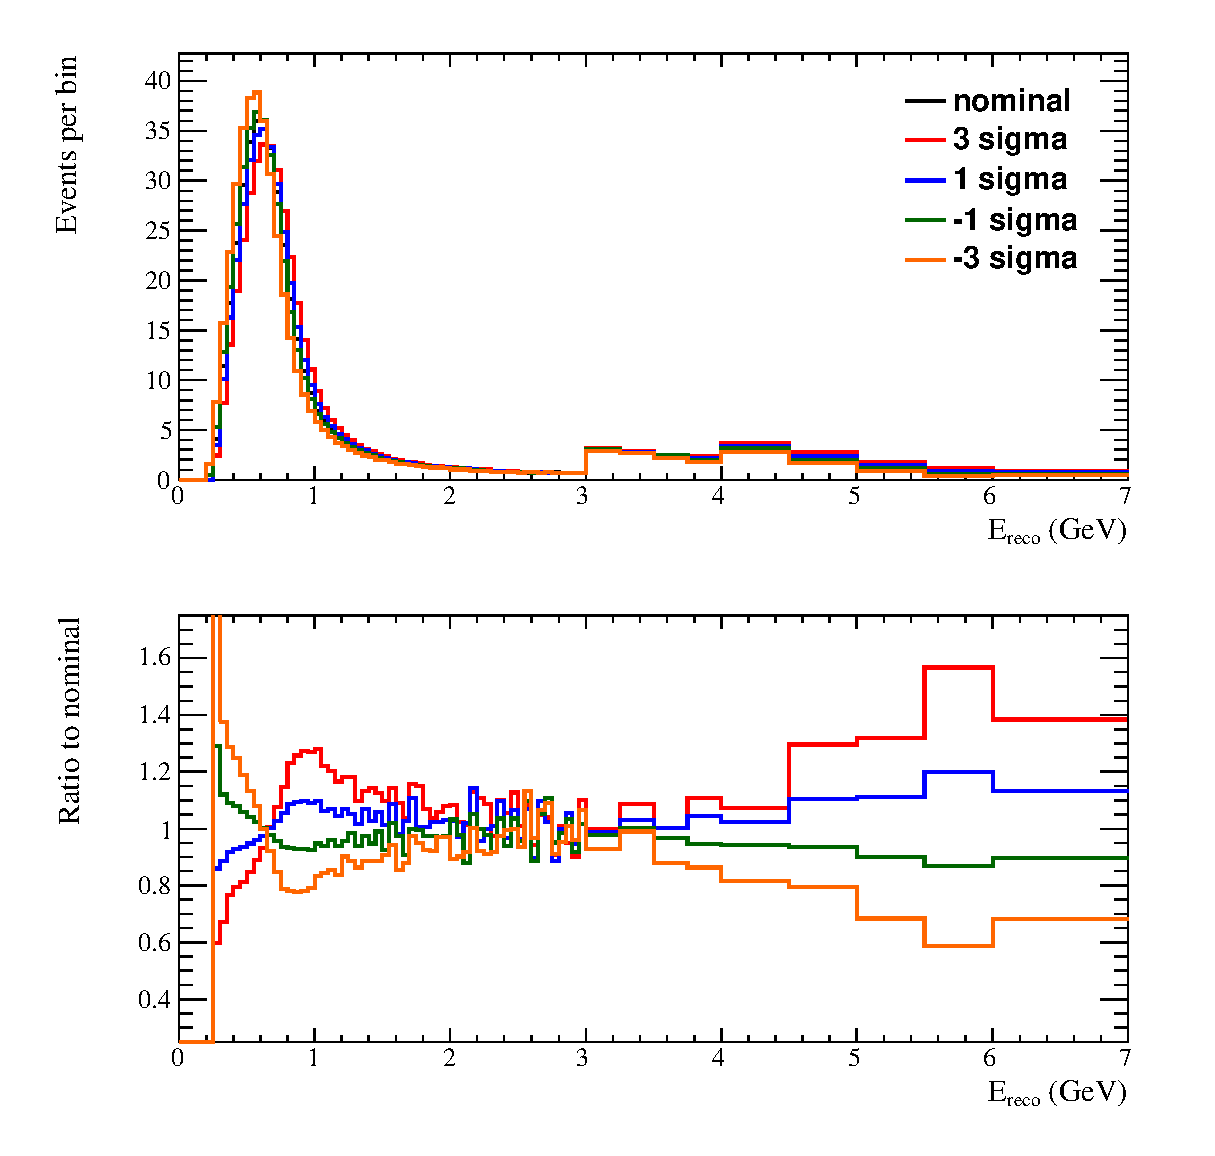
\includegraphics{./images/spectrum_tweaked/unoscillated/ereco_twk_f_sk_e_scale}}
\caption
{ Effect of $f_{E; r}^{SK}$   for no oscillations (all mixing angles set to 0). }
\label{fig:noosc_ereco_twk_f_sk_e_scale}
\end{center}
\end{figure}
\clearpage

\begin{figure}
\begin{center}
\resizebox{14cm}{!}{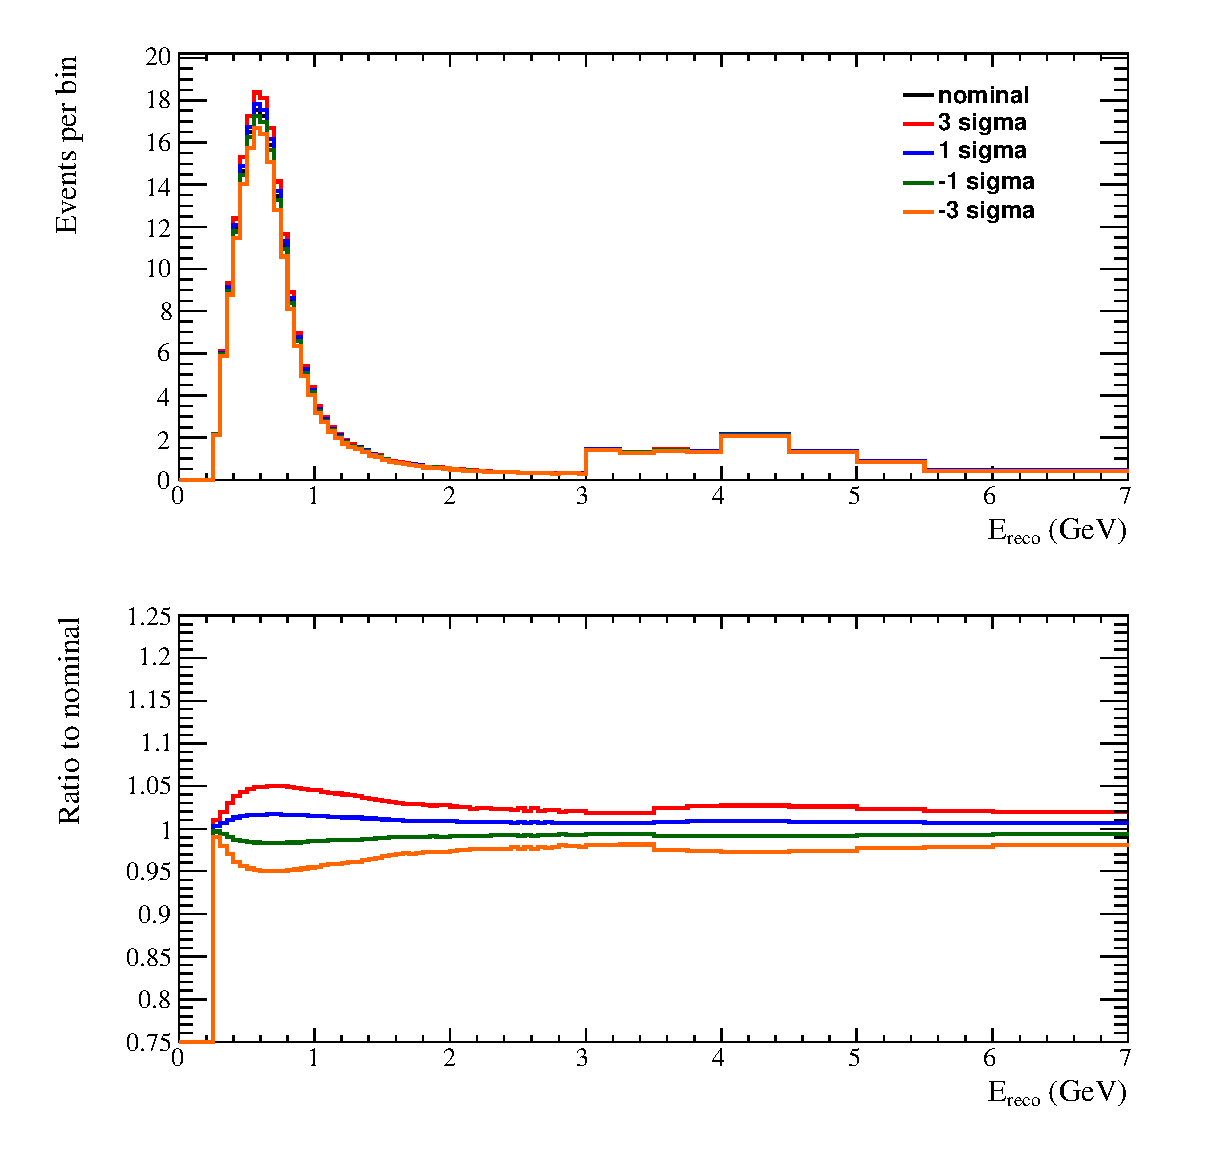
\includegraphics{./images/spectrum_tweaked/unoscillated/ereco_twk_f_sk_eff_1Rmu_ccqe_oth}}
\caption
{ Effect of $f_{CCQEoth; r}^{SK}$ for no oscillations (all mixing angles set to 0). }
\label{fig:noosc_ereco_twk_f_sk_eff_1Rmu_ccqe_oth}
\end{center}
\end{figure}
\clearpage

\begin{figure}
\begin{center}
\resizebox{14cm}{!}{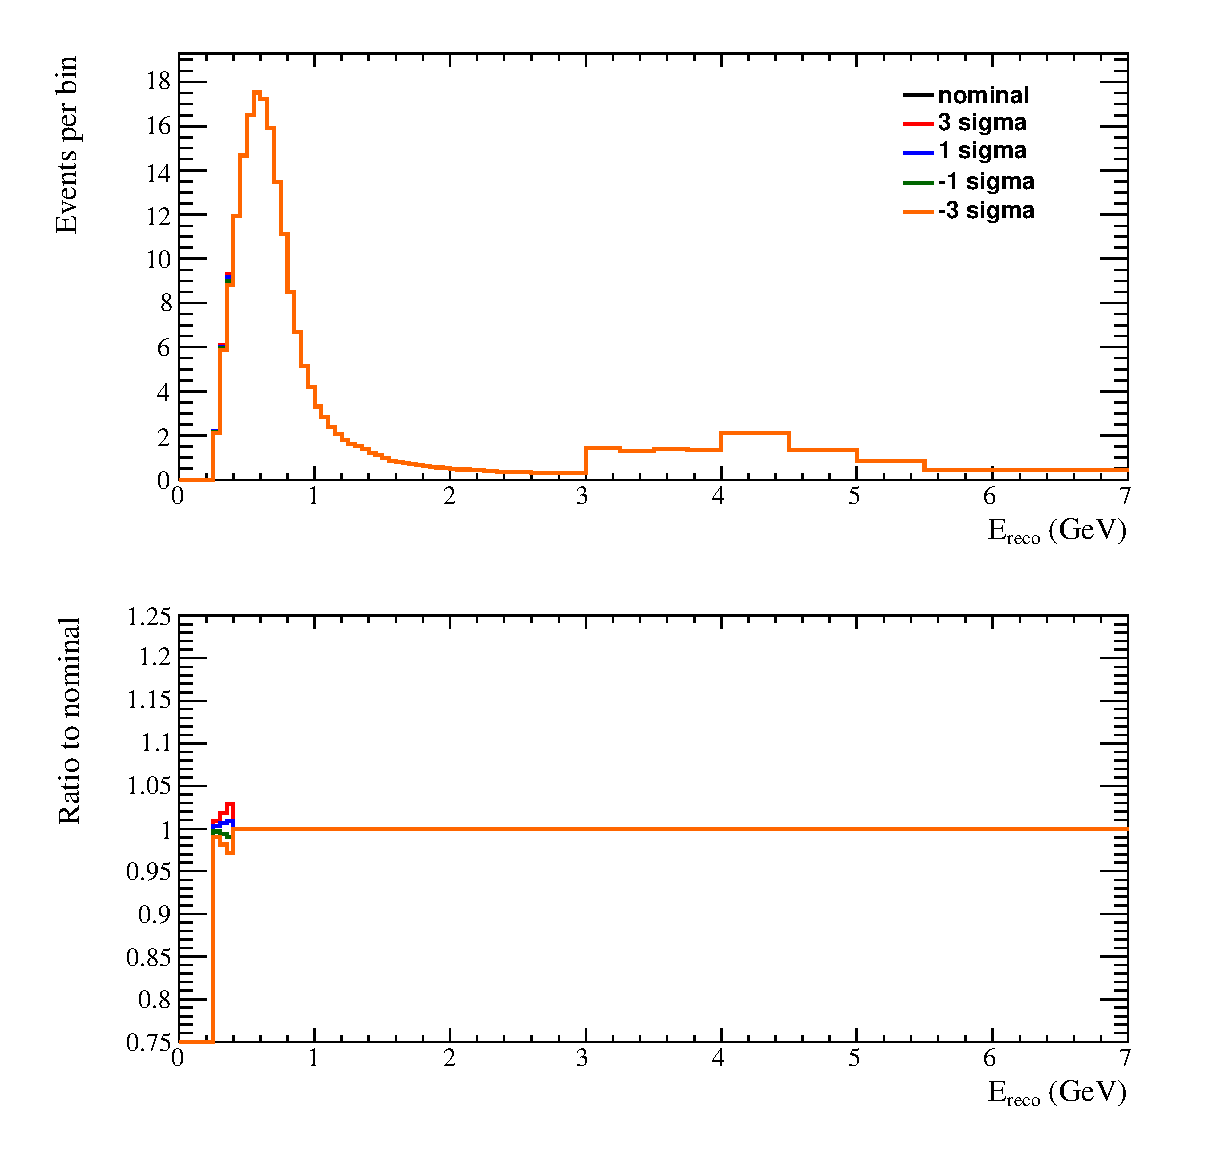
\includegraphics{./images/spectrum_tweaked/unoscillated/ereco_twk_f_sk_eff_1Rmu_ccqe_rc0}}
\caption
{ Effect of $f_{CCQERC0; r}^{SK}$ for no oscillations (all mixing angles set to 0). }
\label{fig:noosc_ereco_twk_f_sk_eff_1Rmu_ccqe_rc0}
\end{center}
\end{figure}
\clearpage

\begin{figure}
\begin{center}
\resizebox{14cm}{!}{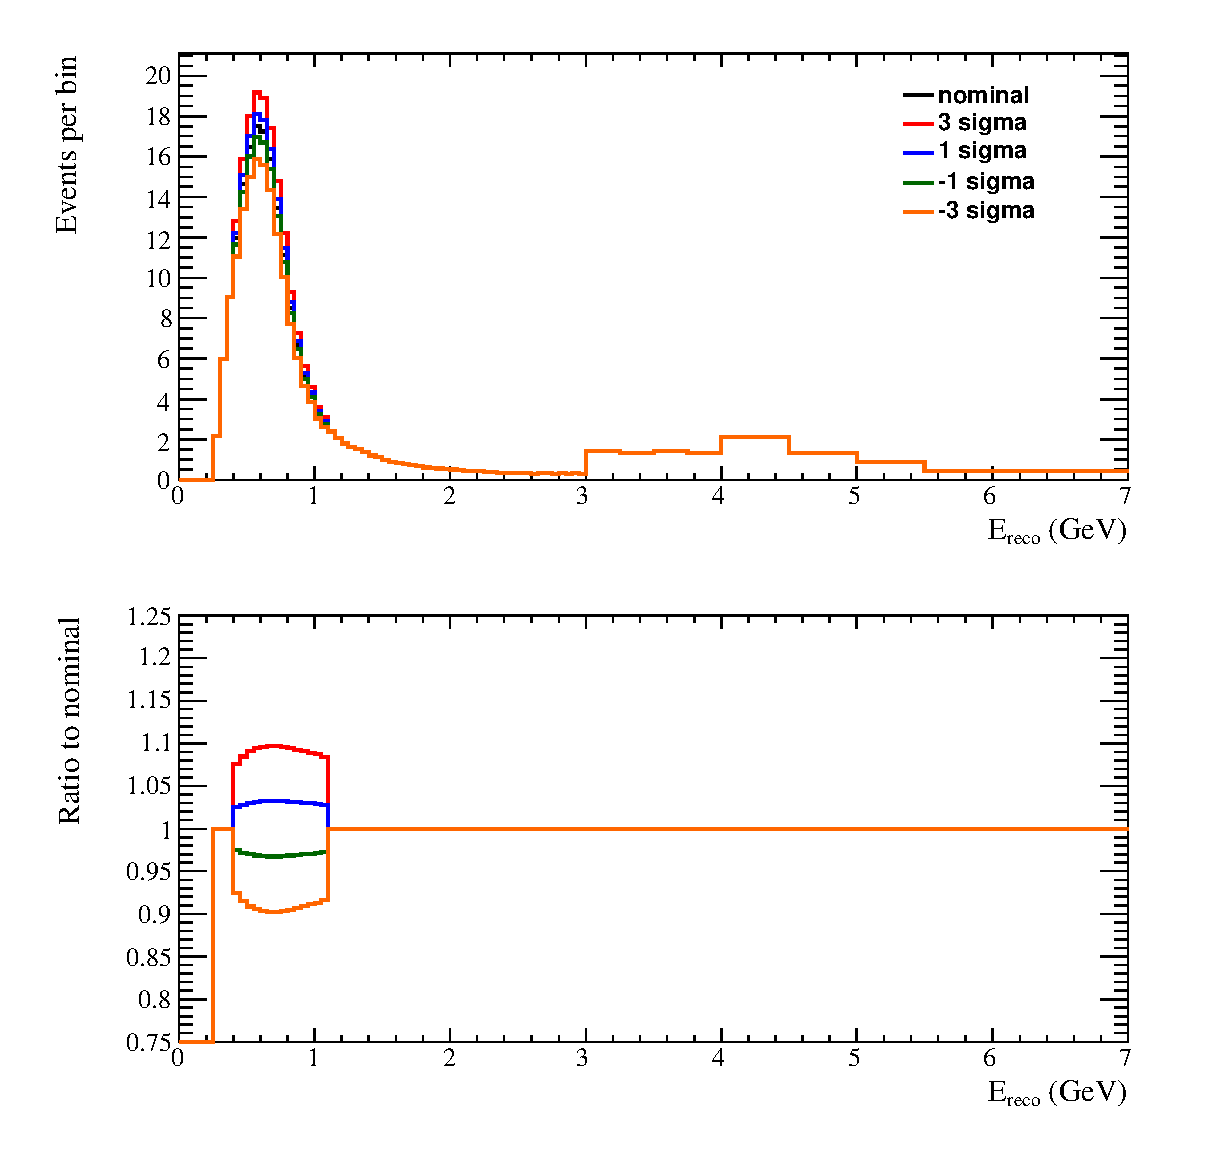
\includegraphics{./images/spectrum_tweaked/unoscillated/ereco_twk_f_sk_eff_1Rmu_ccqe_rc1}}
\caption
{ Effect of $f_{CCQERC1; r}^{SK}$ for no oscillations (all mixing angles set to 0). }
\label{fig:noosc_ereco_twk_f_sk_eff_1Rmu_ccqe_rc1}
\end{center}
\end{figure}
\clearpage

\begin{figure}
\begin{center}
\resizebox{14cm}{!}{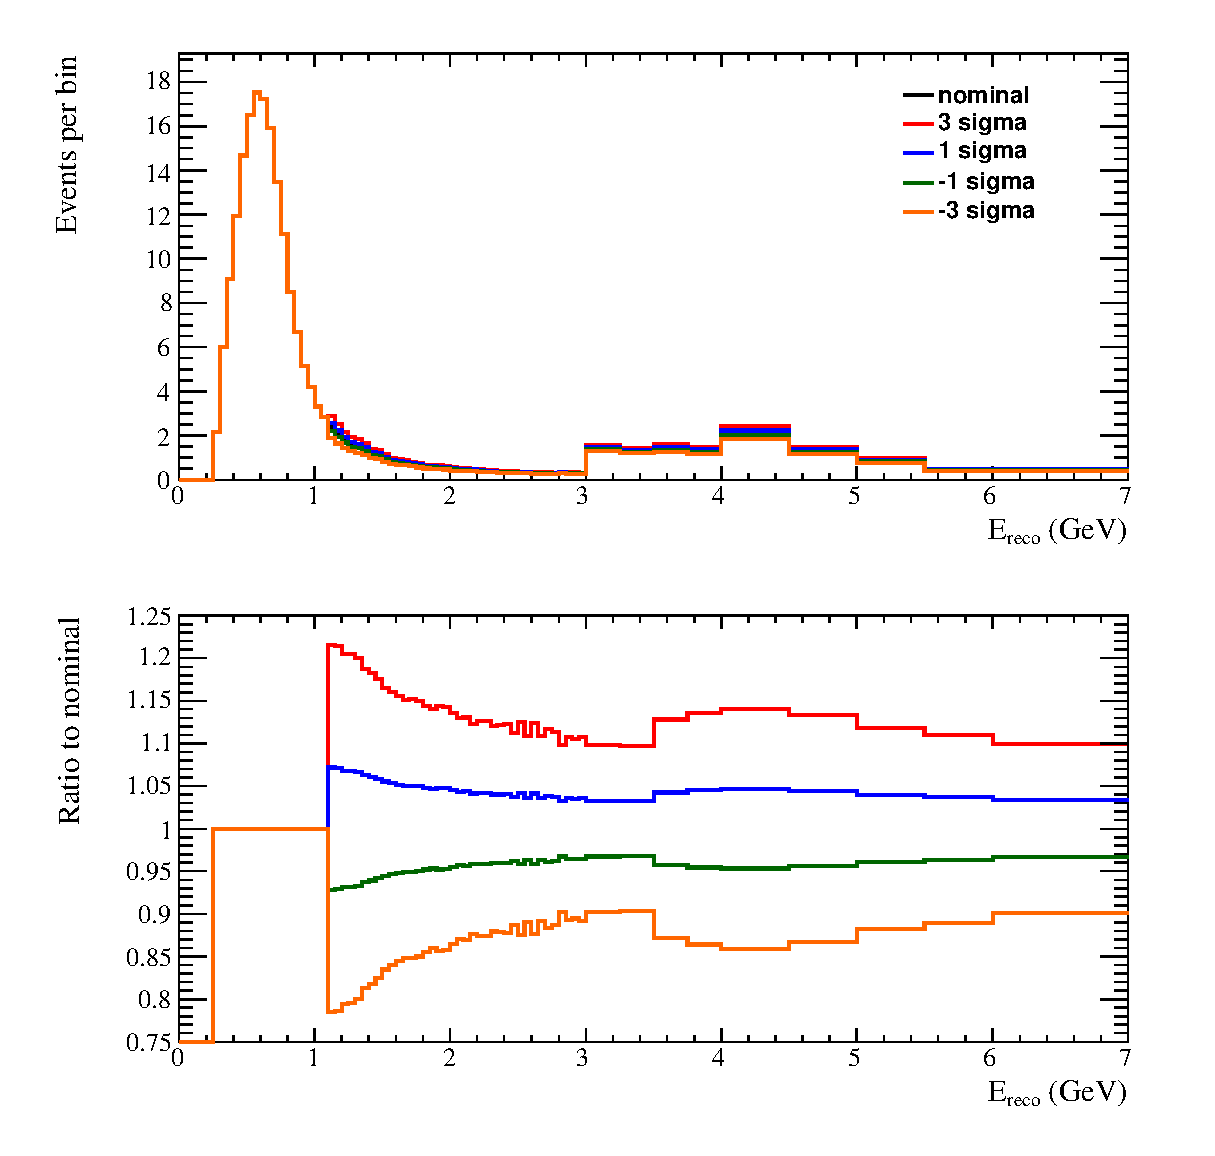
\includegraphics{./images/spectrum_tweaked/unoscillated/ereco_twk_f_sk_eff_1Rmu_ccqe_rc2}}
\caption
{ Effect of $f_{CCQERC2; r}^{SK}$ for no oscillations (all mixing angles set to 0). }
\label{fig:noosc_ereco_twk_f_sk_eff_1Rmu_ccqe_rc2}
\end{center}
\end{figure}
\clearpage

\begin{figure}
\begin{center}
\resizebox{14cm}{!}{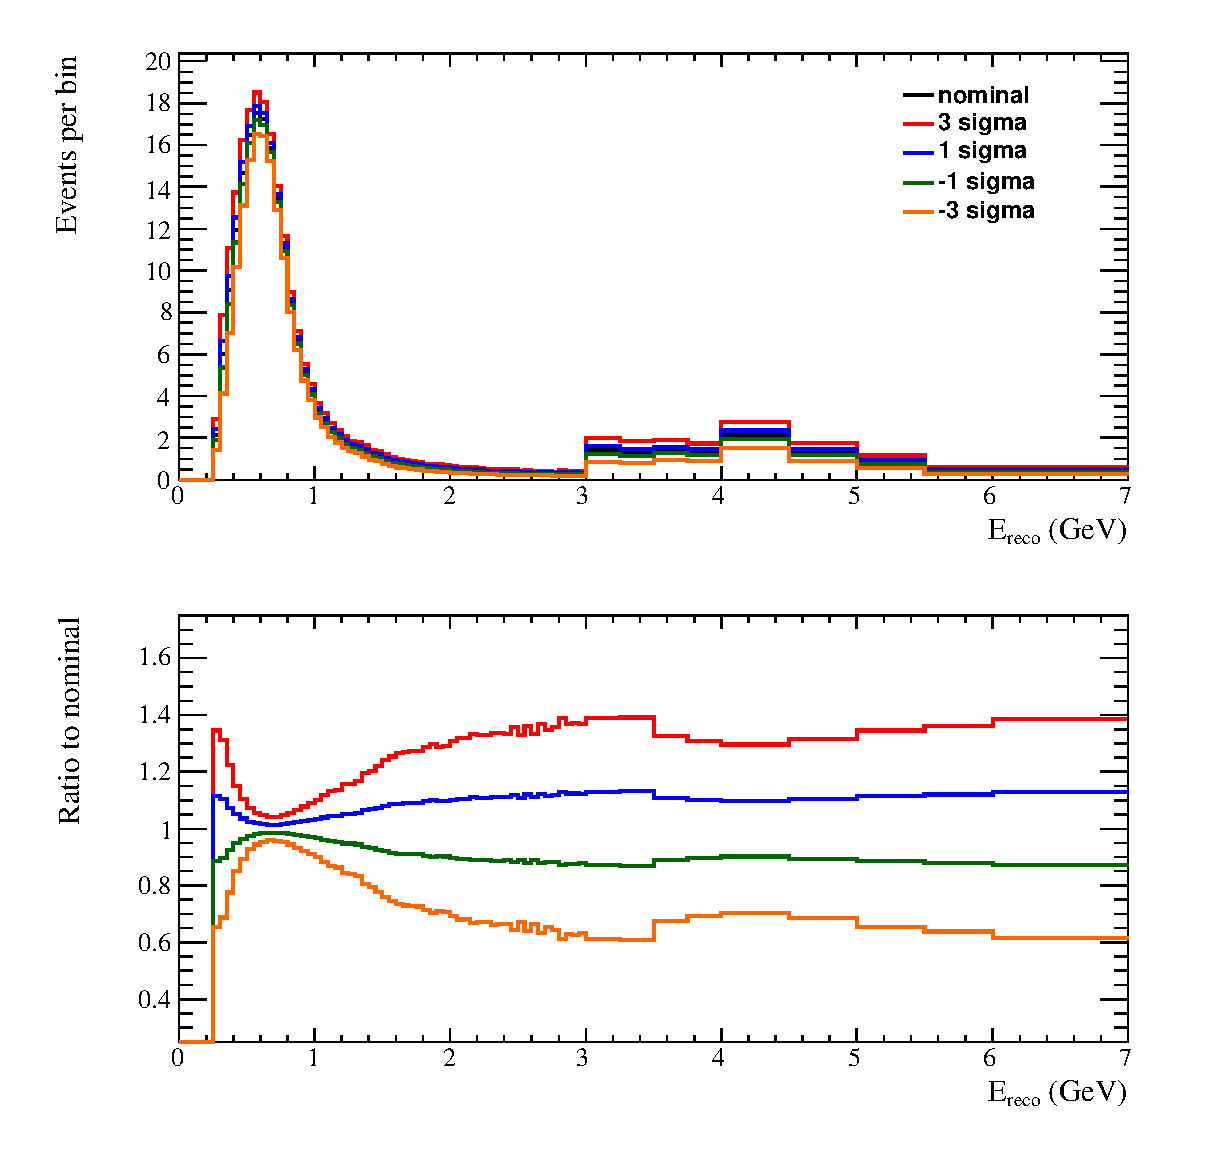
\includegraphics{./images/spectrum_tweaked/unoscillated/ereco_twk_f_sk_eff_1Rmu_ccnonqe}}
\caption
{ Effect of $f_{CCnQE; r}^{SK}$ for no oscillations (all mixing angles set to 0). }
\label{fig:noosc_ereco_twk_f_sk_eff_1Rmu_ccnonqe}
\end{center}
\end{figure}
\clearpage

\begin{figure}
\begin{center}
\resizebox{14cm}{!}{\includegraphics{./images/spectrum_tweaked/unoscillated/ereco_twk_f_sk_eff_1Rmu_nc}}
\caption
{ Effect of $f_{NC; r}^{SK}$ for no oscillations (all mixing angles set to 0). }
\label{fig:noosc_ereco_twk_f_sk_eff_1Rmu_nc}
\end{center}
\end{figure}
\clearpage

\begin{figure}
\begin{center}
\resizebox{14cm}{!}{\includegraphics{./images/spectrum_tweaked/unoscillated/ereco_twk_f_sk_eff_1Rmu_nuecc}}
\caption
{ Effect of $f_{\nu_e; r}^{SK}$ for no oscillations (all mixing angles set to 0). }
\label{fig:noosc_ereco_twk_f_sk_eff_1Rmu_nuecc}
\end{center}
\end{figure}
\clearpage

\begin{figure}
\begin{center}
\resizebox{14cm}{!}{\includegraphics{./images/spectrum_tweaked/unoscillated/ereco_twk_f_banff00}}
\caption
{ Effect of $f_{0; t, r}^{banff}$ for no oscillations (all mixing angles set to 0). }
\label{fig:noosc_ereco_twk_f_banff00}
\end{center}
\end{figure}
\clearpage

\begin{figure}
\begin{center}
\resizebox{14cm}{!}{\includegraphics{./images/spectrum_tweaked/unoscillated/ereco_twk_f_banff01}}
\caption
{ Effect of $f_{1; t, r}^{banff}$ for no oscillations (all mixing angles set to 0). }
\label{fig:noosc_ereco_twk_f_banff01}
\end{center}
\end{figure}
\clearpage

\begin{figure}
\begin{center}
\resizebox{14cm}{!}{\includegraphics{./images/spectrum_tweaked/unoscillated/ereco_twk_f_banff02}}
\caption
{ Effect of $f_{2; t, r}^{banff}$ for no oscillations (all mixing angles set to 0). }
\label{fig:noosc_ereco_twk_f_banff02}
\end{center}
\end{figure}
\clearpage

\begin{figure}
\begin{center}
\resizebox{14cm}{!}{\includegraphics{./images/spectrum_tweaked/unoscillated/ereco_twk_f_banff03}}
\caption
{ Effect of $f_{3; t, r}^{banff}$ for no oscillations (all mixing angles set to 0). }
\label{fig:noosc_ereco_twk_f_banff03}
\end{center}
\end{figure}
\clearpage

\begin{figure}
\begin{center}
\resizebox{14cm}{!}{\includegraphics{./images/spectrum_tweaked/unoscillated/ereco_twk_f_banff04}}
\caption
{ Effect of $f_{4; t, r}^{banff}$ for no oscillations (all mixing angles set to 0). }
\label{fig:noosc_ereco_twk_f_banff04}
\end{center}
\end{figure}
\clearpage

\begin{figure}
\begin{center}
\resizebox{14cm}{!}{\includegraphics{./images/spectrum_tweaked/unoscillated/ereco_twk_f_banff05}}
\caption
{ Effect of $f_{5; t, r}^{banff}$ for no oscillations (all mixing angles set to 0). }
\label{fig:noosc_ereco_twk_f_banff05}
\end{center}
\end{figure}
\clearpage

\begin{figure}
\begin{center}
\resizebox{14cm}{!}{\includegraphics{./images/spectrum_tweaked/unoscillated/ereco_twk_f_banff06}}
\caption
{ Effect of $f_{6; t, r}^{banff}$ for no oscillations (all mixing angles set to 0). }
\label{fig:noosc_ereco_twk_f_banff06}
\end{center}
\end{figure}
\clearpage

\begin{figure}
\begin{center}
\resizebox{14cm}{!}{\includegraphics{./images/spectrum_tweaked/unoscillated/ereco_twk_f_banff07}}
\caption
{ Effect of $f_{7; t, r}^{banff}$ for no oscillations (all mixing angles set to 0). }
\label{fig:noosc_ereco_twk_f_banff07}
\end{center}
\end{figure}
\clearpage

\begin{figure}
\begin{center}
\resizebox{14cm}{!}{\includegraphics{./images/spectrum_tweaked/unoscillated/ereco_twk_f_banff08}}
\caption
{ Effect of $f_{8; t, r}^{banff}$ for no oscillations (all mixing angles set to 0). }
\label{fig:noosc_ereco_twk_f_banff08}
\end{center}
\end{figure}
\clearpage

\begin{figure}
\begin{center}
\resizebox{14cm}{!}{\includegraphics{./images/spectrum_tweaked/unoscillated/ereco_twk_f_banff09}}
\caption
{ Effect of $f_{9; t, r}^{banff}$ for no oscillations (all mixing angles set to 0). }
\label{fig:noosc_ereco_twk_f_banff09}
\end{center}
\end{figure}
\clearpage

\begin{figure}
\begin{center}
\resizebox{14cm}{!}{\includegraphics{./images/spectrum_tweaked/unoscillated/ereco_twk_f_banff10}}
\caption
{ Effect of $f_{10; t, r}^{banff}$ for no oscillations (all mixing angles set to 0). }
\label{fig:noosc_ereco_twk_f_banff10}
\end{center}
\end{figure}
\clearpage

\begin{figure}
\begin{center}
\resizebox{14cm}{!}{\includegraphics{./images/spectrum_tweaked/unoscillated/ereco_twk_f_banff11}}
\caption
{ Effect of $f_{11; t, r}^{banff}$ for no oscillations (all mixing angles set to 0). }
\label{fig:noosc_ereco_twk_f_banff11}
\end{center}
\end{figure}
\clearpage

\begin{figure}
\begin{center}
\resizebox{14cm}{!}{\includegraphics{./images/spectrum_tweaked/unoscillated/ereco_twk_f_banff12}}
\caption
{ Effect of $f_{12; t, r}^{banff}$ for no oscillations (all mixing angles set to 0). }
\label{fig:noosc_ereco_twk_f_banff12}
\end{center}
\end{figure}
\clearpage

\begin{figure}
\begin{center}
\resizebox{14cm}{!}{\includegraphics{./images/spectrum_tweaked/unoscillated/ereco_twk_f_banff13}}
\caption
{ Effect of $f_{13; t, r}^{banff}$ for no oscillations (all mixing angles set to 0). }
\label{fig:noosc_ereco_twk_f_banff13}
\end{center}
\end{figure}
\clearpage

\begin{figure}
\begin{center}
\resizebox{14cm}{!}{\includegraphics{./images/spectrum_tweaked/unoscillated/ereco_twk_f_banff14}}
\caption
{ Effect of $f_{14; t, r}^{banff}$ for no oscillations (all mixing angles set to 0). }
\label{fig:noosc_ereco_twk_f_banff14}
\end{center}
\end{figure}
\clearpage

\begin{figure}
\begin{center}
\resizebox{14cm}{!}{\includegraphics{./images/spectrum_tweaked/unoscillated/ereco_twk_f_banff15}}
\caption
{ Effect of $f_{15; t, r}^{banff}$ for no oscillations (all mixing angles set to 0). }
\label{fig:noosc_ereco_twk_f_banff15}
\end{center}
\end{figure}
\clearpage

\begin{figure}
\begin{center}
\resizebox{14cm}{!}{\includegraphics{./images/spectrum_tweaked/unoscillated/ereco_twk_f_banffmaqe}}
\caption
{ Effect of $f_{16; t, r}^{banff}$ for no oscillations (all mixing angles set to 0). }
\label{fig:noosc_ereco_twk_f_banffmaqe}
\end{center}
\end{figure}
\clearpage

\begin{figure}
\begin{center}
\resizebox{14cm}{!}{\includegraphics{./images/spectrum_tweaked/unoscillated/ereco_twk_f_banffmares}}
\caption
{ Effect of $f_{17; t, r}^{banff}$ for no oscillations (all mixing angles set to 0). }
\label{fig:noosc_ereco_twk_f_banffmares}
\end{center}
\end{figure}
\clearpage

\begin{figure}
\begin{center}
\resizebox{14cm}{!}{\includegraphics{./images/spectrum_tweaked/unoscillated/ereco_twk_f_banffccqee0}}
\caption
{ Effect of $f_{18; t, r}^{banff}$ for no oscillations (all mixing angles set to 0). }
\label{fig:noosc_ereco_twk_f_banffccqee0}
\end{center}
\end{figure}
\clearpage

\begin{figure}
\begin{center}
\resizebox{14cm}{!}{\includegraphics{./images/spectrum_tweaked/unoscillated/ereco_twk_f_banffccqee1}}
\caption
{ Effect of $f_{19; t, r}^{banff}$ for no oscillations (all mixing angles set to 0). }
\label{fig:noosc_ereco_twk_f_banffccqee1}
\end{center}
\end{figure}
\clearpage

\begin{figure}
\begin{center}
\resizebox{14cm}{!}{\includegraphics{./images/spectrum_tweaked/unoscillated/ereco_twk_f_banffccqee2}}
\caption
{ Effect of $f_{20; t, r}^{banff}$ for no oscillations (all mixing angles set to 0). }
\label{fig:noosc_ereco_twk_f_banffccqee2}
\end{center}
\end{figure}
\clearpage

\begin{figure}
\begin{center}
\resizebox{14cm}{!}{\includegraphics{./images/spectrum_tweaked/unoscillated/ereco_twk_f_banffcc1pie0}}
\caption
{ Effect of $f_{21; t, r}^{banff}$ for no oscillations (all mixing angles set to 0). }
\label{fig:noosc_ereco_twk_f_banffcc1pie0}
\end{center}
\end{figure}
\clearpage

\begin{figure}
\begin{center}
\resizebox{14cm}{!}{\includegraphics{./images/spectrum_tweaked/unoscillated/ereco_twk_f_banffcc1pie1}}
\caption
{ Effect of $f_{22; t, r}^{banff}$ for no oscillations (all mixing angles set to 0). }
\label{fig:noosc_ereco_twk_f_banffcc1pie1}
\end{center}
\end{figure}
\clearpage

\begin{figure}
\begin{center}
\resizebox{14cm}{!}{\includegraphics{./images/spectrum_tweaked/unoscillated/ereco_twk_f_pfermi}}
\caption
{ Effect of $f_{pF; t, r}$ for no oscillations (all mixing angles set to 0). }
\label{fig:noosc_ereco_twk_f_pfermi}
\end{center}
\end{figure}
\clearpage

\begin{figure}
\begin{center}
\resizebox{14cm}{!}{\includegraphics{./images/spectrum_tweaked/unoscillated/ereco_twk_f_specfunc}}
\caption
{ Effect of $f_{SF; t, r}$ for no oscillations (all mixing angles set to 0). }
\label{fig:noosc_ereco_twk_f_specfunc}
\end{center}
\end{figure}
\clearpage

\begin{figure}
\begin{center}
\resizebox{14cm}{!}{\includegraphics{./images/spectrum_tweaked/unoscillated/ereco_twk_f_wshape}}
\caption
{ Effect of $f_{Wshape; t, r}$ for no oscillations (all mixing angles set to 0). }
\label{fig:noosc_ereco_twk_f_wshape}
\end{center}
\end{figure}
\clearpage

\begin{figure}
\begin{center}
\resizebox{14cm}{!}{\includegraphics{./images/spectrum_tweaked/unoscillated/ereco_twk_f_shapeCCoth}}
\caption
{ Effect of $f_{CCothShape; t, r}$ for no oscillations (all mixing angles set to 0). }
\label{fig:noosc_ereco_twk_f_shapeCCoth}
\end{center}
\end{figure}
\clearpage

\begin{figure}
\begin{center}
\resizebox{14cm}{!}{\includegraphics{./images/spectrum_tweaked/unoscillated/ereco_twk_f_pilessdelta}}
\caption
{ Effect of $f_{\pi-less\Delta; t, r}$ for no oscillations (all mixing angles set to 0). }
\label{fig:noosc_ereco_twk_f_pilessdelta}
\end{center}
\end{figure}
\clearpage

\begin{figure}
\begin{center}
\resizebox{14cm}{!}{\includegraphics{./images/spectrum_tweaked/unoscillated/ereco_twk_f_bindE}}
\caption
{ Effect of $f_{bindE; t, r}$ for no oscillations (all mixing angles set to 0). }
\label{fig:noosc_ereco_twk_f_bindE}
\end{center}
\end{figure}
\clearpage

\begin{figure}
\begin{center}
\resizebox{14cm}{!}{\includegraphics{./images/spectrum_tweaked/unoscillated/ereco_twk_f_norm_cccoh}}
\caption
{ Effect of $f_{CCcoh; t}$ for no oscillations (all mixing angles set to 0). }
\label{fig:noosc_ereco_twk_f_norm_cccoh}
\end{center}
\end{figure}
\clearpage

\begin{figure}
\begin{center}
\resizebox{14cm}{!}{\includegraphics{./images/spectrum_tweaked/unoscillated/ereco_twk_f_norm_nc1piC}}
\caption
{ Effect of $f_{NC1\pi^\pm; t}$ for no oscillations (all mixing angles set to 0). }
\label{fig:noosc_ereco_twk_f_norm_nc1piC}
\end{center}
\end{figure}
\clearpage

\begin{figure}
\begin{center}
\resizebox{14cm}{!}{\includegraphics{./images/spectrum_tweaked/unoscillated/ereco_twk_f_norm_ncoth}}
\caption
{ Effect of $f_{NCoth; t}$ for no oscillations (all mixing angles set to 0). }
\label{fig:noosc_ereco_twk_f_norm_ncoth}
\end{center}
\end{figure}
\clearpage

\begin{figure}
\begin{center}
\resizebox{14cm}{!}{\includegraphics{./images/spectrum_tweaked/unoscillated/ereco_twk_f_norm_nuetonumu}}
\caption
{ Effect of $f_{CC\nu_e; t}$ for no oscillations (all mixing angles set to 0). }
\label{fig:noosc_ereco_twk_f_norm_nuetonumu}
\end{center}
\end{figure}
\clearpage

\begin{figure}
\begin{center}
\resizebox{14cm}{!}{\includegraphics{./images/spectrum_tweaked/unoscillated/ereco_twk_f_norm_antinutonu}}
\caption
{ Effect of $f_{CC\bar{\nu}; t}$ for no oscillations (all mixing angles set to 0). }
\label{fig:noosc_ereco_twk_f_norm_antinutonu}
\end{center}
\end{figure}
\clearpage

\begin{figure}
\begin{center}
\resizebox{14cm}{!}{\includegraphics{./images/spectrum_tweaked/unoscillated/ereco_twk_f_fsi000}}
\caption
{ Effect of $f_{0; t, r}^{FSI}$ for no oscillations (all mixing angles set to 0). }
\label{fig:noosc_ereco_twk_f_fsi000}
\end{center}
\end{figure}
\clearpage

\begin{figure}
\begin{center}
\resizebox{14cm}{!}{\includegraphics{./images/spectrum_tweaked/unoscillated/ereco_twk_f_fsi001}}
\caption
{ Effect of $f_{1; t, r}^{FSI}$ for no oscillations (all mixing angles set to 0). }
\label{fig:noosc_ereco_twk_f_fsi001}
\end{center}
\end{figure}
\clearpage

\begin{figure}
\begin{center}
\resizebox{14cm}{!}{\includegraphics{./images/spectrum_tweaked/unoscillated/ereco_twk_f_fsi002}}
\caption
{ Effect of $f_{2; t, r}^{FSI}$ for no oscillations (all mixing angles set to 0). }
\label{fig:noosc_ereco_twk_f_fsi002}
\end{center}
\end{figure}
\clearpage

\begin{figure}
\begin{center}
\resizebox{14cm}{!}{\includegraphics{./images/spectrum_tweaked/unoscillated/ereco_twk_f_fsi003}}
\caption
{ Effect of $f_{3; t, r}^{FSI}$ for no oscillations (all mixing angles set to 0). }
\label{fig:noosc_ereco_twk_f_fsi003}
\end{center}
\end{figure}
\clearpage

\begin{figure}
\begin{center}
\resizebox{14cm}{!}{\includegraphics{./images/spectrum_tweaked/unoscillated/ereco_twk_f_fsi004}}
\caption
{ Effect of $f_{4; t, r}^{FSI}$ for no oscillations (all mixing angles set to 0). }
\label{fig:noosc_ereco_twk_f_fsi004}
\end{center}
\end{figure}
\clearpage

\begin{figure}
\begin{center}
\resizebox{14cm}{!}{\includegraphics{./images/spectrum_tweaked/unoscillated/ereco_twk_f_fsi005}}
\caption
{ Effect of $f_{5; t, r}^{FSI}$ for no oscillations (all mixing angles set to 0). }
\label{fig:noosc_ereco_twk_f_fsi005}
\end{center}
\end{figure}
\clearpage



\begin{figure}
\begin{center}
\resizebox{14cm}{!}{\includegraphics{./images/spectrum_tweaked/oscillated/ereco_twk_f_sk_e_scale}}
\caption
{ Effect of $f_{E; r}^{SK}$   for 3 flavour oscillations, using oscillation parameters:  $\sin^22\theta_{12} = $0.857; $\sin^22\theta_{13} = $0.098; $\sin^22\theta_{23} = $1; $\delta_{CP} = $        0; $\Delta m^2_{12} = $    7.5e-05; $\Delta m^2_{32} = $    0.0024. }
\label{fig:osc_ereco_twk_f_sk_e_scale}
\end{center}
\end{figure}
\clearpage

\begin{figure}
\begin{center}
\resizebox{14cm}{!}{\includegraphics{./images/spectrum_tweaked/oscillated/ereco_twk_f_sk_eff_1Rmu_ccqe_oth}}
\caption
{ Effect of $f_{CCQEoth; r}^{SK}$ for 3 flavour oscillations, using oscillation parameters:  $\sin^22\theta_{12} = $0.857; $\sin^22\theta_{13} = $0.098; $\sin^22\theta_{23} = $1; $\delta_{CP} = $        0; $\Delta m^2_{12} = $    7.5e-05; $\Delta m^2_{32} = $    0.0024. }
\label{fig:osc_ereco_twk_f_sk_eff_1Rmu_ccqe_oth}
\end{center}
\end{figure}
\clearpage

\begin{figure}
\begin{center}
\resizebox{14cm}{!}{\includegraphics{./images/spectrum_tweaked/oscillated/ereco_twk_f_sk_eff_1Rmu_ccqe_rc0}}
\caption
{ Effect of $f_{CCQERC0; r}^{SK}$ for 3 flavour oscillations, using oscillation parameters:  $\sin^22\theta_{12} = $0.857; $\sin^22\theta_{13} = $0.098; $\sin^22\theta_{23} = $1; $\delta_{CP} = $        0; $\Delta m^2_{12} = $    7.5e-05; $\Delta m^2_{32} = $    0.0024. }
\label{fig:osc_ereco_twk_f_sk_eff_1Rmu_ccqe_rc0}
\end{center}
\end{figure}
\clearpage

\begin{figure}
\begin{center}
\resizebox{14cm}{!}{\includegraphics{./images/spectrum_tweaked/oscillated/ereco_twk_f_sk_eff_1Rmu_ccqe_rc1}}
\caption
{ Effect of $f_{CCQERC1; r}^{SK}$ for 3 flavour oscillations, using oscillation parameters:  $\sin^22\theta_{12} = $0.857; $\sin^22\theta_{13} = $0.098; $\sin^22\theta_{23} = $1; $\delta_{CP} = $        0; $\Delta m^2_{12} = $    7.5e-05; $\Delta m^2_{32} = $    0.0024. }
\label{fig:osc_ereco_twk_f_sk_eff_1Rmu_ccqe_rc1}
\end{center}
\end{figure}
\clearpage

\begin{figure}
\begin{center}
\resizebox{14cm}{!}{\includegraphics{./images/spectrum_tweaked/oscillated/ereco_twk_f_sk_eff_1Rmu_ccqe_rc2}}
\caption
{ Effect of $f_{CCQERC2; r}^{SK}$ for 3 flavour oscillations, using oscillation parameters:  $\sin^22\theta_{12} = $0.857; $\sin^22\theta_{13} = $0.098; $\sin^22\theta_{23} = $1; $\delta_{CP} = $        0; $\Delta m^2_{12} = $    7.5e-05; $\Delta m^2_{32} = $    0.0024. }
\label{fig:osc_ereco_twk_f_sk_eff_1Rmu_ccqe_rc2}
\end{center}
\end{figure}
\clearpage

\begin{figure}
\begin{center}
\resizebox{14cm}{!}{\includegraphics{./images/spectrum_tweaked/oscillated/ereco_twk_f_sk_eff_1Rmu_ccnonqe}}
\caption
{ Effect of $f_{CCnQE; r}^{SK}$ for 3 flavour oscillations, using oscillation parameters:  $\sin^22\theta_{12} = $0.857; $\sin^22\theta_{13} = $0.098; $\sin^22\theta_{23} = $1; $\delta_{CP} = $        0; $\Delta m^2_{12} = $    7.5e-05; $\Delta m^2_{32} = $    0.0024. }
\label{fig:osc_ereco_twk_f_sk_eff_1Rmu_ccnonqe}
\end{center}
\end{figure}
\clearpage

\begin{figure}
\begin{center}
\resizebox{14cm}{!}{\includegraphics{./images/spectrum_tweaked/oscillated/ereco_twk_f_sk_eff_1Rmu_nc}}
\caption
{ Effect of $f_{NC; r}^{SK}$ for 3 flavour oscillations, using oscillation parameters:  $\sin^22\theta_{12} = $0.857; $\sin^22\theta_{13} = $0.098; $\sin^22\theta_{23} = $1; $\delta_{CP} = $        0; $\Delta m^2_{12} = $    7.5e-05; $\Delta m^2_{32} = $    0.0024. }
\label{fig:osc_ereco_twk_f_sk_eff_1Rmu_nc}
\end{center}
\end{figure}
\clearpage

\begin{figure}
\begin{center}
\resizebox{14cm}{!}{\includegraphics{./images/spectrum_tweaked/oscillated/ereco_twk_f_sk_eff_1Rmu_nuecc}}
\caption
{ Effect of $f_{\nu_e; r}^{SK}$ for 3 flavour oscillations, using oscillation parameters:  $\sin^22\theta_{12} = $0.857; $\sin^22\theta_{13} = $0.098; $\sin^22\theta_{23} = $1; $\delta_{CP} = $        0; $\Delta m^2_{12} = $    7.5e-05; $\Delta m^2_{32} = $    0.0024. }
\label{fig:osc_ereco_twk_f_sk_eff_1Rmu_nuecc}
\end{center}
\end{figure}
\clearpage

\begin{figure}
\begin{center}
\resizebox{14cm}{!}{\includegraphics{./images/spectrum_tweaked/oscillated/ereco_twk_f_banff00}}
\caption
{ Effect of $f_{0; t, r}^{banff}$ for 3 flavour oscillations, using oscillation parameters:  $\sin^22\theta_{12} = $0.857; $\sin^22\theta_{13} = $0.098; $\sin^22\theta_{23} = $1; $\delta_{CP} = $        0; $\Delta m^2_{12} = $    7.5e-05; $\Delta m^2_{32} = $    0.0024. }
\label{fig:osc_ereco_twk_f_banff00}
\end{center}
\end{figure}
\clearpage

\begin{figure}
\begin{center}
\resizebox{14cm}{!}{\includegraphics{./images/spectrum_tweaked/oscillated/ereco_twk_f_banff01}}
\caption
{ Effect of $f_{1; t, r}^{banff}$ for 3 flavour oscillations, using oscillation parameters:  $\sin^22\theta_{12} = $0.857; $\sin^22\theta_{13} = $0.098; $\sin^22\theta_{23} = $1; $\delta_{CP} = $        0; $\Delta m^2_{12} = $    7.5e-05; $\Delta m^2_{32} = $    0.0024. }
\label{fig:osc_ereco_twk_f_banff01}
\end{center}
\end{figure}
\clearpage

\begin{figure}
\begin{center}
\resizebox{14cm}{!}{\includegraphics{./images/spectrum_tweaked/oscillated/ereco_twk_f_banff02}}
\caption
{ Effect of $f_{2; t, r}^{banff}$ for 3 flavour oscillations, using oscillation parameters:  $\sin^22\theta_{12} = $0.857; $\sin^22\theta_{13} = $0.098; $\sin^22\theta_{23} = $1; $\delta_{CP} = $        0; $\Delta m^2_{12} = $    7.5e-05; $\Delta m^2_{32} = $    0.0024. }
\label{fig:osc_ereco_twk_f_banff02}
\end{center}
\end{figure}
\clearpage

\begin{figure}
\begin{center}
\resizebox{14cm}{!}{\includegraphics{./images/spectrum_tweaked/oscillated/ereco_twk_f_banff03}}
\caption
{ Effect of $f_{3; t, r}^{banff}$ for 3 flavour oscillations, using oscillation parameters:  $\sin^22\theta_{12} = $0.857; $\sin^22\theta_{13} = $0.098; $\sin^22\theta_{23} = $1; $\delta_{CP} = $        0; $\Delta m^2_{12} = $    7.5e-05; $\Delta m^2_{32} = $    0.0024. }
\label{fig:osc_ereco_twk_f_banff03}
\end{center}
\end{figure}
\clearpage

\begin{figure}
\begin{center}
\resizebox{14cm}{!}{\includegraphics{./images/spectrum_tweaked/oscillated/ereco_twk_f_banff04}}
\caption
{ Effect of $f_{4; t, r}^{banff}$ for 3 flavour oscillations, using oscillation parameters:  $\sin^22\theta_{12} = $0.857; $\sin^22\theta_{13} = $0.098; $\sin^22\theta_{23} = $1; $\delta_{CP} = $        0; $\Delta m^2_{12} = $    7.5e-05; $\Delta m^2_{32} = $    0.0024. }
\label{fig:osc_ereco_twk_f_banff04}
\end{center}
\end{figure}
\clearpage

\begin{figure}
\begin{center}
\resizebox{14cm}{!}{\includegraphics{./images/spectrum_tweaked/oscillated/ereco_twk_f_banff05}}
\caption
{ Effect of $f_{5; t, r}^{banff}$ for 3 flavour oscillations, using oscillation parameters:  $\sin^22\theta_{12} = $0.857; $\sin^22\theta_{13} = $0.098; $\sin^22\theta_{23} = $1; $\delta_{CP} = $        0; $\Delta m^2_{12} = $    7.5e-05; $\Delta m^2_{32} = $    0.0024. }
\label{fig:osc_ereco_twk_f_banff05}
\end{center}
\end{figure}
\clearpage

\begin{figure}
\begin{center}
\resizebox{14cm}{!}{\includegraphics{./images/spectrum_tweaked/oscillated/ereco_twk_f_banff06}}
\caption
{ Effect of $f_{6; t, r}^{banff}$ for 3 flavour oscillations, using oscillation parameters:  $\sin^22\theta_{12} = $0.857; $\sin^22\theta_{13} = $0.098; $\sin^22\theta_{23} = $1; $\delta_{CP} = $        0; $\Delta m^2_{12} = $    7.5e-05; $\Delta m^2_{32} = $    0.0024. }
\label{fig:osc_ereco_twk_f_banff06}
\end{center}
\end{figure}
\clearpage

\begin{figure}
\begin{center}
\resizebox{14cm}{!}{\includegraphics{./images/spectrum_tweaked/oscillated/ereco_twk_f_banff07}}
\caption
{ Effect of $f_{7; t, r}^{banff}$ for 3 flavour oscillations, using oscillation parameters:  $\sin^22\theta_{12} = $0.857; $\sin^22\theta_{13} = $0.098; $\sin^22\theta_{23} = $1; $\delta_{CP} = $        0; $\Delta m^2_{12} = $    7.5e-05; $\Delta m^2_{32} = $    0.0024. }
\label{fig:osc_ereco_twk_f_banff07}
\end{center}
\end{figure}
\clearpage

\begin{figure}
\begin{center}
\resizebox{14cm}{!}{\includegraphics{./images/spectrum_tweaked/oscillated/ereco_twk_f_banff08}}
\caption
{ Effect of $f_{8; t, r}^{banff}$ for 3 flavour oscillations, using oscillation parameters:  $\sin^22\theta_{12} = $0.857; $\sin^22\theta_{13} = $0.098; $\sin^22\theta_{23} = $1; $\delta_{CP} = $        0; $\Delta m^2_{12} = $    7.5e-05; $\Delta m^2_{32} = $    0.0024. }
\label{fig:osc_ereco_twk_f_banff08}
\end{center}
\end{figure}
\clearpage

\begin{figure}
\begin{center}
\resizebox{14cm}{!}{\includegraphics{./images/spectrum_tweaked/oscillated/ereco_twk_f_banff09}}
\caption
{ Effect of $f_{9; t, r}^{banff}$ for 3 flavour oscillations, using oscillation parameters:  $\sin^22\theta_{12} = $0.857; $\sin^22\theta_{13} = $0.098; $\sin^22\theta_{23} = $1; $\delta_{CP} = $        0; $\Delta m^2_{12} = $    7.5e-05; $\Delta m^2_{32} = $    0.0024. }
\label{fig:osc_ereco_twk_f_banff09}
\end{center}
\end{figure}
\clearpage

\begin{figure}
\begin{center}
\resizebox{14cm}{!}{\includegraphics{./images/spectrum_tweaked/oscillated/ereco_twk_f_banff10}}
\caption
{ Effect of $f_{10; t, r}^{banff}$ for 3 flavour oscillations, using oscillation parameters:  $\sin^22\theta_{12} = $0.857; $\sin^22\theta_{13} = $0.098; $\sin^22\theta_{23} = $1; $\delta_{CP} = $        0; $\Delta m^2_{12} = $    7.5e-05; $\Delta m^2_{32} = $    0.0024. }
\label{fig:osc_ereco_twk_f_banff10}
\end{center}
\end{figure}
\clearpage

\begin{figure}
\begin{center}
\resizebox{14cm}{!}{\includegraphics{./images/spectrum_tweaked/oscillated/ereco_twk_f_banff11}}
\caption
{ Effect of $f_{11; t, r}^{banff}$ for 3 flavour oscillations, using oscillation parameters:  $\sin^22\theta_{12} = $0.857; $\sin^22\theta_{13} = $0.098; $\sin^22\theta_{23} = $1; $\delta_{CP} = $        0; $\Delta m^2_{12} = $    7.5e-05; $\Delta m^2_{32} = $    0.0024. }
\label{fig:osc_ereco_twk_f_banff11}
\end{center}
\end{figure}
\clearpage

\begin{figure}
\begin{center}
\resizebox{14cm}{!}{\includegraphics{./images/spectrum_tweaked/oscillated/ereco_twk_f_banff12}}
\caption
{ Effect of $f_{12; t, r}^{banff}$ for 3 flavour oscillations, using oscillation parameters:  $\sin^22\theta_{12} = $0.857; $\sin^22\theta_{13} = $0.098; $\sin^22\theta_{23} = $1; $\delta_{CP} = $        0; $\Delta m^2_{12} = $    7.5e-05; $\Delta m^2_{32} = $    0.0024. }
\label{fig:osc_ereco_twk_f_banff12}
\end{center}
\end{figure}
\clearpage

\begin{figure}
\begin{center}
\resizebox{14cm}{!}{\includegraphics{./images/spectrum_tweaked/oscillated/ereco_twk_f_banff13}}
\caption
{ Effect of $f_{13; t, r}^{banff}$ for 3 flavour oscillations, using oscillation parameters:  $\sin^22\theta_{12} = $0.857; $\sin^22\theta_{13} = $0.098; $\sin^22\theta_{23} = $1; $\delta_{CP} = $        0; $\Delta m^2_{12} = $    7.5e-05; $\Delta m^2_{32} = $    0.0024. }
\label{fig:osc_ereco_twk_f_banff13}
\end{center}
\end{figure}
\clearpage

\begin{figure}
\begin{center}
\resizebox{14cm}{!}{\includegraphics{./images/spectrum_tweaked/oscillated/ereco_twk_f_banff14}}
\caption
{ Effect of $f_{14; t, r}^{banff}$ for 3 flavour oscillations, using oscillation parameters:  $\sin^22\theta_{12} = $0.857; $\sin^22\theta_{13} = $0.098; $\sin^22\theta_{23} = $1; $\delta_{CP} = $        0; $\Delta m^2_{12} = $    7.5e-05; $\Delta m^2_{32} = $    0.0024. }
\label{fig:osc_ereco_twk_f_banff14}
\end{center}
\end{figure}
\clearpage

\begin{figure}
\begin{center}
\resizebox{14cm}{!}{\includegraphics{./images/spectrum_tweaked/oscillated/ereco_twk_f_banff15}}
\caption
{ Effect of $f_{15; t, r}^{banff}$ for 3 flavour oscillations, using oscillation parameters:  $\sin^22\theta_{12} = $0.857; $\sin^22\theta_{13} = $0.098; $\sin^22\theta_{23} = $1; $\delta_{CP} = $        0; $\Delta m^2_{12} = $    7.5e-05; $\Delta m^2_{32} = $    0.0024. }
\label{fig:osc_ereco_twk_f_banff15}
\end{center}
\end{figure}
\clearpage

\begin{figure}
\begin{center}
\resizebox{14cm}{!}{\includegraphics{./images/spectrum_tweaked/oscillated/ereco_twk_f_banffmaqe}}
\caption
{ Effect of $f_{16; t, r}^{banff}$ for 3 flavour oscillations, using oscillation parameters:  $\sin^22\theta_{12} = $0.857; $\sin^22\theta_{13} = $0.098; $\sin^22\theta_{23} = $1; $\delta_{CP} = $        0; $\Delta m^2_{12} = $    7.5e-05; $\Delta m^2_{32} = $    0.0024. }
\label{fig:osc_ereco_twk_f_banffmaqe}
\end{center}
\end{figure}
\clearpage

\begin{figure}
\begin{center}
\resizebox{14cm}{!}{\includegraphics{./images/spectrum_tweaked/oscillated/ereco_twk_f_banffmares}}
\caption
{ Effect of $f_{17; t, r}^{banff}$ for 3 flavour oscillations, using oscillation parameters:  $\sin^22\theta_{12} = $0.857; $\sin^22\theta_{13} = $0.098; $\sin^22\theta_{23} = $1; $\delta_{CP} = $        0; $\Delta m^2_{12} = $    7.5e-05; $\Delta m^2_{32} = $    0.0024. }
\label{fig:osc_ereco_twk_f_banffmares}
\end{center}
\end{figure}
\clearpage

\begin{figure}
\begin{center}
\resizebox{14cm}{!}{\includegraphics{./images/spectrum_tweaked/oscillated/ereco_twk_f_banffccqee0}}
\caption
{ Effect of $f_{18; t, r}^{banff}$ for 3 flavour oscillations, using oscillation parameters:  $\sin^22\theta_{12} = $0.857; $\sin^22\theta_{13} = $0.098; $\sin^22\theta_{23} = $1; $\delta_{CP} = $        0; $\Delta m^2_{12} = $    7.5e-05; $\Delta m^2_{32} = $    0.0024. }
\label{fig:osc_ereco_twk_f_banffccqee0}
\end{center}
\end{figure}
\clearpage

\begin{figure}
\begin{center}
\resizebox{14cm}{!}{\includegraphics{./images/spectrum_tweaked/oscillated/ereco_twk_f_banffccqee1}}
\caption
{ Effect of $f_{19; t, r}^{banff}$ for 3 flavour oscillations, using oscillation parameters:  $\sin^22\theta_{12} = $0.857; $\sin^22\theta_{13} = $0.098; $\sin^22\theta_{23} = $1; $\delta_{CP} = $        0; $\Delta m^2_{12} = $    7.5e-05; $\Delta m^2_{32} = $    0.0024. }
\label{fig:osc_ereco_twk_f_banffccqee1}
\end{center}
\end{figure}
\clearpage

\begin{figure}
\begin{center}
\resizebox{14cm}{!}{\includegraphics{./images/spectrum_tweaked/oscillated/ereco_twk_f_banffccqee2}}
\caption
{ Effect of $f_{20; t, r}^{banff}$ for 3 flavour oscillations, using oscillation parameters:  $\sin^22\theta_{12} = $0.857; $\sin^22\theta_{13} = $0.098; $\sin^22\theta_{23} = $1; $\delta_{CP} = $        0; $\Delta m^2_{12} = $    7.5e-05; $\Delta m^2_{32} = $    0.0024. }
\label{fig:osc_ereco_twk_f_banffccqee2}
\end{center}
\end{figure}
\clearpage

\begin{figure}
\begin{center}
\resizebox{14cm}{!}{\includegraphics{./images/spectrum_tweaked/oscillated/ereco_twk_f_banffcc1pie0}}
\caption
{ Effect of $f_{21; t, r}^{banff}$ for 3 flavour oscillations, using oscillation parameters:  $\sin^22\theta_{12} = $0.857; $\sin^22\theta_{13} = $0.098; $\sin^22\theta_{23} = $1; $\delta_{CP} = $        0; $\Delta m^2_{12} = $    7.5e-05; $\Delta m^2_{32} = $    0.0024. }
\label{fig:osc_ereco_twk_f_banffcc1pie0}
\end{center}
\end{figure}
\clearpage

\begin{figure}
\begin{center}
\resizebox{14cm}{!}{\includegraphics{./images/spectrum_tweaked/oscillated/ereco_twk_f_banffcc1pie1}}
\caption
{ Effect of $f_{22; t, r}^{banff}$ for 3 flavour oscillations, using oscillation parameters:  $\sin^22\theta_{12} = $0.857; $\sin^22\theta_{13} = $0.098; $\sin^22\theta_{23} = $1; $\delta_{CP} = $        0; $\Delta m^2_{12} = $    7.5e-05; $\Delta m^2_{32} = $    0.0024. }
\label{fig:osc_ereco_twk_f_banffcc1pie1}
\end{center}
\end{figure}
\clearpage

\begin{figure}
\begin{center}
\resizebox{14cm}{!}{\includegraphics{./images/spectrum_tweaked/oscillated/ereco_twk_f_pfermi}}
\caption
{ Effect of $f_{pF; t, r}$ for 3 flavour oscillations, using oscillation parameters:  $\sin^22\theta_{12} = $0.857; $\sin^22\theta_{13} = $0.098; $\sin^22\theta_{23} = $1; $\delta_{CP} = $        0; $\Delta m^2_{12} = $    7.5e-05; $\Delta m^2_{32} = $    0.0024. }
\label{fig:osc_ereco_twk_f_pfermi}
\end{center}
\end{figure}
\clearpage

\begin{figure}
\begin{center}
\resizebox{14cm}{!}{\includegraphics{./images/spectrum_tweaked/oscillated/ereco_twk_f_specfunc}}
\caption
{ Effect of $f_{SF; t, r}$ for 3 flavour oscillations, using oscillation parameters:  $\sin^22\theta_{12} = $0.857; $\sin^22\theta_{13} = $0.098; $\sin^22\theta_{23} = $1; $\delta_{CP} = $        0; $\Delta m^2_{12} = $    7.5e-05; $\Delta m^2_{32} = $    0.0024. }
\label{fig:osc_ereco_twk_f_specfunc}
\end{center}
\end{figure}
\clearpage

\begin{figure}
\begin{center}
\resizebox{14cm}{!}{\includegraphics{./images/spectrum_tweaked/oscillated/ereco_twk_f_wshape}}
\caption
{ Effect of $f_{Wshape; t, r}$ for 3 flavour oscillations, using oscillation parameters:  $\sin^22\theta_{12} = $0.857; $\sin^22\theta_{13} = $0.098; $\sin^22\theta_{23} = $1; $\delta_{CP} = $        0; $\Delta m^2_{12} = $    7.5e-05; $\Delta m^2_{32} = $    0.0024. }
\label{fig:osc_ereco_twk_f_wshape}
\end{center}
\end{figure}
\clearpage

\begin{figure}
\begin{center}
\resizebox{14cm}{!}{\includegraphics{./images/spectrum_tweaked/oscillated/ereco_twk_f_shapeCCoth}}
\caption
{ Effect of $f_{CCothShape; t, r}$ for 3 flavour oscillations, using oscillation parameters:  $\sin^22\theta_{12} = $0.857; $\sin^22\theta_{13} = $0.098; $\sin^22\theta_{23} = $1; $\delta_{CP} = $        0; $\Delta m^2_{12} = $    7.5e-05; $\Delta m^2_{32} = $    0.0024. }
\label{fig:osc_ereco_twk_f_shapeCCoth}
\end{center}
\end{figure}
\clearpage

\begin{figure}
\begin{center}
\resizebox{14cm}{!}{\includegraphics{./images/spectrum_tweaked/oscillated/ereco_twk_f_pilessdelta}}
\caption
{ Effect of $f_{\pi-less\Delta; t, r}$ for 3 flavour oscillations, using oscillation parameters:  $\sin^22\theta_{12} = $0.857; $\sin^22\theta_{13} = $0.098; $\sin^22\theta_{23} = $1; $\delta_{CP} = $        0; $\Delta m^2_{12} = $    7.5e-05; $\Delta m^2_{32} = $    0.0024. }
\label{fig:osc_ereco_twk_f_pilessdelta}
\end{center}
\end{figure}
\clearpage

\begin{figure}
\begin{center}
\resizebox{14cm}{!}{\includegraphics{./images/spectrum_tweaked/oscillated/ereco_twk_f_bindE}}
\caption
{ Effect of $f_{bindE; t, r}$ for 3 flavour oscillations, using oscillation parameters:  $\sin^22\theta_{12} = $0.857; $\sin^22\theta_{13} = $0.098; $\sin^22\theta_{23} = $1; $\delta_{CP} = $        0; $\Delta m^2_{12} = $    7.5e-05; $\Delta m^2_{32} = $    0.0024. }
\label{fig:osc_ereco_twk_f_bindE}
\end{center}
\end{figure}
\clearpage

\begin{figure}
\begin{center}
\resizebox{14cm}{!}{\includegraphics{./images/spectrum_tweaked/oscillated/ereco_twk_f_norm_cccoh}}
\caption
{ Effect of $f_{CCcoh; t}$ for 3 flavour oscillations, using oscillation parameters:  $\sin^22\theta_{12} = $0.857; $\sin^22\theta_{13} = $0.098; $\sin^22\theta_{23} = $1; $\delta_{CP} = $        0; $\Delta m^2_{12} = $    7.5e-05; $\Delta m^2_{32} = $    0.0024. }
\label{fig:osc_ereco_twk_f_norm_cccoh}
\end{center}
\end{figure}
\clearpage

\begin{figure}
\begin{center}
\resizebox{14cm}{!}{\includegraphics{./images/spectrum_tweaked/oscillated/ereco_twk_f_norm_nc1piC}}
\caption
{ Effect of $f_{NC1\pi^\pm; t}$ for 3 flavour oscillations, using oscillation parameters:  $\sin^22\theta_{12} = $0.857; $\sin^22\theta_{13} = $0.098; $\sin^22\theta_{23} = $1; $\delta_{CP} = $        0; $\Delta m^2_{12} = $    7.5e-05; $\Delta m^2_{32} = $    0.0024. }
\label{fig:osc_ereco_twk_f_norm_nc1piC}
\end{center}
\end{figure}
\clearpage

\begin{figure}
\begin{center}
\resizebox{14cm}{!}{\includegraphics{./images/spectrum_tweaked/oscillated/ereco_twk_f_norm_ncoth}}
\caption
{ Effect of $f_{NCoth; t}$ for 3 flavour oscillations, using oscillation parameters:  $\sin^22\theta_{12} = $0.857; $\sin^22\theta_{13} = $0.098; $\sin^22\theta_{23} = $1; $\delta_{CP} = $        0; $\Delta m^2_{12} = $    7.5e-05; $\Delta m^2_{32} = $    0.0024. }
\label{fig:osc_ereco_twk_f_norm_ncoth}
\end{center}
\end{figure}
\clearpage

\begin{figure}
\begin{center}
\resizebox{14cm}{!}{\includegraphics{./images/spectrum_tweaked/oscillated/ereco_twk_f_norm_nuetonumu}}
\caption
{ Effect of $f_{CC\nu_e; t}$ for 3 flavour oscillations, using oscillation parameters:  $\sin^22\theta_{12} = $0.857; $\sin^22\theta_{13} = $0.098; $\sin^22\theta_{23} = $1; $\delta_{CP} = $        0; $\Delta m^2_{12} = $    7.5e-05; $\Delta m^2_{32} = $    0.0024. }
\label{fig:osc_ereco_twk_f_norm_nuetonumu}
\end{center}
\end{figure}
\clearpage

\begin{figure}
\begin{center}
\resizebox{14cm}{!}{\includegraphics{./images/spectrum_tweaked/oscillated/ereco_twk_f_norm_antinutonu}}
\caption
{ Effect of $f_{CC\bar{\nu}; t}$ for 3 flavour oscillations, using oscillation parameters:  $\sin^22\theta_{12} = $0.857; $\sin^22\theta_{13} = $0.098; $\sin^22\theta_{23} = $1; $\delta_{CP} = $        0; $\Delta m^2_{12} = $    7.5e-05; $\Delta m^2_{32} = $    0.0024. }
\label{fig:osc_ereco_twk_f_norm_antinutonu}
\end{center}
\end{figure}
\clearpage

\begin{figure}
\begin{center}
\resizebox{14cm}{!}{\includegraphics{./images/spectrum_tweaked/oscillated/ereco_twk_f_fsi000}}
\caption
{ Effect of $f_{0; t, r}^{FSI}$ for 3 flavour oscillations, using oscillation parameters:  $\sin^22\theta_{12} = $0.857; $\sin^22\theta_{13} = $0.098; $\sin^22\theta_{23} = $1; $\delta_{CP} = $        0; $\Delta m^2_{12} = $    7.5e-05; $\Delta m^2_{32} = $    0.0024. }
\label{fig:osc_ereco_twk_f_fsi000}
\end{center}
\end{figure}
\clearpage

\begin{figure}
\begin{center}
\resizebox{14cm}{!}{\includegraphics{./images/spectrum_tweaked/oscillated/ereco_twk_f_fsi001}}
\caption
{ Effect of $f_{1; t, r}^{FSI}$ for 3 flavour oscillations, using oscillation parameters:  $\sin^22\theta_{12} = $0.857; $\sin^22\theta_{13} = $0.098; $\sin^22\theta_{23} = $1; $\delta_{CP} = $        0; $\Delta m^2_{12} = $    7.5e-05; $\Delta m^2_{32} = $    0.0024. }
\label{fig:osc_ereco_twk_f_fsi001}
\end{center}
\end{figure}
\clearpage

\begin{figure}
\begin{center}
\resizebox{14cm}{!}{\includegraphics{./images/spectrum_tweaked/oscillated/ereco_twk_f_fsi002}}
\caption
{ Effect of $f_{2; t, r}^{FSI}$ for 3 flavour oscillations, using oscillation parameters:  $\sin^22\theta_{12} = $0.857; $\sin^22\theta_{13} = $0.098; $\sin^22\theta_{23} = $1; $\delta_{CP} = $        0; $\Delta m^2_{12} = $    7.5e-05; $\Delta m^2_{32} = $    0.0024. }
\label{fig:osc_ereco_twk_f_fsi002}
\end{center}
\end{figure}
\clearpage

\begin{figure}
\begin{center}
\resizebox{14cm}{!}{\includegraphics{./images/spectrum_tweaked/oscillated/ereco_twk_f_fsi003}}
\caption
{ Effect of $f_{3; t, r}^{FSI}$ for 3 flavour oscillations, using oscillation parameters:  $\sin^22\theta_{12} = $0.857; $\sin^22\theta_{13} = $0.098; $\sin^22\theta_{23} = $1; $\delta_{CP} = $        0; $\Delta m^2_{12} = $    7.5e-05; $\Delta m^2_{32} = $    0.0024. }
\label{fig:osc_ereco_twk_f_fsi003}
\end{center}
\end{figure}
\clearpage

\begin{figure}
\begin{center}
\resizebox{14cm}{!}{\includegraphics{./images/spectrum_tweaked/oscillated/ereco_twk_f_fsi004}}
\caption
{ Effect of $f_{4; t, r}^{FSI}$ for 3 flavour oscillations, using oscillation parameters:  $\sin^22\theta_{12} = $0.857; $\sin^22\theta_{13} = $0.098; $\sin^22\theta_{23} = $1; $\delta_{CP} = $        0; $\Delta m^2_{12} = $    7.5e-05; $\Delta m^2_{32} = $    0.0024. }
\label{fig:osc_ereco_twk_f_fsi004}
\end{center}
\end{figure}
\clearpage

\begin{figure}
\begin{center}
\resizebox{14cm}{!}{\includegraphics{./images/spectrum_tweaked/oscillated/ereco_twk_f_fsi005}}
\caption
{ Effect of $f_{5; t, r}^{FSI}$ for 3 flavour oscillations, using oscillation parameters:  $\sin^22\theta_{12} = $0.857; $\sin^22\theta_{13} = $0.098; $\sin^22\theta_{23} = $1; $\delta_{CP} = $        0; $\Delta m^2_{12} = $    7.5e-05; $\Delta m^2_{32} = $    0.0024. }
\label{fig:osc_ereco_twk_f_fsi005}
\end{center}
\end{figure}
\clearpage





\clearpage

\section{Detailed study of the effect of systematics on the best-fit oscillation parameters}
\label{appendix:systematics_bestfit_oscillations}


This section describes a study into the effect of systematics on the best-fit oscillation parameters.
It was used to determine which systematic parameters to include in the 2+8 fit. Before doing the study, it was decided to include a systematic 
if its effect on the best-fit oscillation parameters is greater than one-quarter the size of the statistical error at one or more oscillation 
parameter points. The statistical error was evaluated using 2+0 fits of 10000 toy experiments with no systematic fluctuations at each 
oscillation parameter point. The oscillation parameter points used in this study are shown in Fig.\ \ref{fig:apdx:starplot_points}.

In the study, a 2+0 fit was done on a toy MC experiment created without statistical fluctuations and with a single systematic parameter 
tweaked by $\pm$1$\sigma$.
For correlated systematic parameters, $\sigma$ was defined as the square root of the corresponding covariance matrix diagonal entry.
The best-fit values of the oscillation parameters from the 2+0 fit are plotted as an arrow whose origin is at the input point of the study.
For ease of reading, no more than 11 systematics are included on a single plot; for this reason, the plots are split into the following categories:
\begin{itemize}
\item parameters used in the 2+8 fit, Figs. \ref{fig:apdx_star_important_0.80_0.0020}-\ref{fig:apdx_star_important_1.00_0.0030};
\item SuperK detector parameters, Figs. \ref{fig:apdx_star_sk_0.80_0.0020}-\ref{fig:apdx_star_sk_1.00_0.0030};
\item BANFF $\nu_\mu$ flux parameters, Figs. \ref{fig:apdx_star_banffnumu_0.80_0.0020}-\ref{fig:apdx_star_banffnumu_1.00_0.0030};
\item BANFF $\bar{\nu_\mu}$ flux parameters, Figs. \ref{fig:apdx_star_banffnumubar_0.80_0.0020}-\ref{fig:apdx_star_banffnumubar_1.00_0.0030};
\item BANFF cross section parameters, Figs. \ref{fig:apdx_star_banffxsec_0.80_0.0020}-\ref{fig:apdx_star_banffxsec_1.00_0.0030};
\item uncorrelated cross section parameters, Figs. \ref{fig:apdx_star_xsec_0.80_0.0020}-\ref{fig:apdx_star_xsec_1.00_0.0030};
\item FSI+SI parameters, Figs. \ref{fig:apdx_star_fsi_0.80_0.0020}-\ref{fig:apdx_star_fsi_1.00_0.0030};
\item non-23 sector oscillation parameters, Figs. \ref{fig:apdx_star_osc_0.80_0.0020}-\ref{fig:apdx_star_osc_1.00_0.0030}.
\end{itemize}

\begin{figure*}[htb]
\center
\includegraphics[width=25pc]{./images/star_plot/star_study_points}
\caption {
 True oscillation parameter points used in the study on the effect of systematics
 on the best-fit oscillation parameters.
}
\label{fig:apdx:starplot_points}
\end{figure*}


\clearpage


\subsection{Parameters used in the 2+8 fit}
\begin{figure*}[htb]
\begin{minipage}[t]{0.48\linewidth}
\center
\includegraphics[width=18pc]{{./images/star_plot/important-0.800000-0.002000_testbig}.eps}
\caption
{ Effect of parameters used in the 2+8 fit on the best fit point, using a 2+0 fit, with a single systematic changed by $\pm$1 sigma. The ellipse shown is one quarter the size of the statistical error. For 3 flavour oscillations, using oscillation parameters:  $\sin^22\theta_{12} = $0.857; $\sin^22\theta_{13} = $0.098; $\sin^22\theta_{23} = $0.8; $\delta_{CP} = $        0; $\Delta m^2_{12} = $    7.5e-05; $\Delta m^2_{32} = $    0.002. }
\label{fig:apdx_star_important_0.80_0.0020}
\end{minipage}
\hspace{0.06\linewidth}
\begin{minipage}[t]{0.48\linewidth}
\center
\includegraphics[width=18pc]{{./images/star_plot/important-0.800000-0.002400_testbig}.eps}
\caption
{ Effect of parameters used in the 2+8 fit on the best fit point, using a 2+0 fit, with a single systematic changed by $\pm$1 sigma. The ellipse shown is one quarter the size of the statistical error. For 3 flavour oscillations, using oscillation parameters:  $\sin^22\theta_{12} = $0.857; $\sin^22\theta_{13} = $0.098; $\sin^22\theta_{23} = $0.8; $\delta_{CP} = $        0; $\Delta m^2_{12} = $    7.5e-05; $\Delta m^2_{32} = $    0.0024. }
\label{fig:apdx_star_important_0.80_0.0024}
\end{minipage}
\vfill
\begin{minipage}[t]{0.48\linewidth}
\center
\includegraphics[width=18pc]{{./images/star_plot/important-0.800000-0.003000_testbig}.eps}
\caption
{ Effect of parameters used in the 2+8 fit on the best fit point, using a 2+0 fit, with a single systematic changed by $\pm$1 sigma. The ellipse shown is one quarter the size of the statistical error. For 3 flavour oscillations, using oscillation parameters:  $\sin^22\theta_{12} = $0.857; $\sin^22\theta_{13} = $0.098; $\sin^22\theta_{23} = $0.8; $\delta_{CP} = $        0; $\Delta m^2_{12} = $    7.5e-05; $\Delta m^2_{32} = $    0.003. }
\label{fig:apdx_star_important_0.80_0.0030}
\end{minipage}
\hspace{0.06\linewidth}
\begin{minipage}[t]{0.48\linewidth}
\center
\includegraphics[width=18pc]{{./images/star_plot/important-0.900000-0.002200_testbig}.eps}
\caption
{ Effect of parameters used in the 2+8 fit on the best fit point, using a 2+0 fit, with a single systematic changed by $\pm$1 sigma. The ellipse shown is one quarter the size of the statistical error. For 3 flavour oscillations, using oscillation parameters:  $\sin^22\theta_{12} = $0.857; $\sin^22\theta_{13} = $0.098; $\sin^22\theta_{23} = $0.9; $\delta_{CP} = $        0; $\Delta m^2_{12} = $    7.5e-05; $\Delta m^2_{32} = $    0.0022. }
\label{fig:apdx_star_important_0.90_0.0022}
\end{minipage}
\end{figure*}
\clearpage
\begin{figure*}[htb]
\begin{minipage}[t]{0.48\linewidth}
\center
\includegraphics[width=18pc]{{./images/star_plot/important-0.900000-0.002400_testbig}.eps}
\caption
{ Effect of parameters used in the 2+8 fit on the best fit point, using a 2+0 fit, with a single systematic changed by $\pm$1 sigma. The ellipse shown is one quarter the size of the statistical error. For 3 flavour oscillations, using oscillation parameters:  $\sin^22\theta_{12} = $0.857; $\sin^22\theta_{13} = $0.098; $\sin^22\theta_{23} = $0.9; $\delta_{CP} = $        0; $\Delta m^2_{12} = $    7.5e-05; $\Delta m^2_{32} = $    0.0024. }
\label{fig:apdx_star_important_0.90_0.0024}
\end{minipage}
\hspace{0.06\linewidth}
\begin{minipage}[t]{0.48\linewidth}
\center
\includegraphics[width=18pc]{{./images/star_plot/important-0.900000-0.002600_testbig}.eps}
\caption
{ Effect of parameters used in the 2+8 fit on the best fit point, using a 2+0 fit, with a single systematic changed by $\pm$1 sigma. The ellipse shown is one quarter the size of the statistical error. For 3 flavour oscillations, using oscillation parameters:  $\sin^22\theta_{12} = $0.857; $\sin^22\theta_{13} = $0.098; $\sin^22\theta_{23} = $0.9; $\delta_{CP} = $        0; $\Delta m^2_{12} = $    7.5e-05; $\Delta m^2_{32} = $    0.0026. }
\label{fig:apdx_star_important_0.90_0.0026}
\end{minipage}
\vfill
\begin{minipage}[t]{0.48\linewidth}
\center
\includegraphics[width=18pc]{{./images/star_plot/important-0.950000-0.002200_testbig}.eps}
\caption
{ Effect of parameters used in the 2+8 fit on the best fit point, using a 2+0 fit, with a single systematic changed by $\pm$1 sigma. The ellipse shown is one quarter the size of the statistical error. For 3 flavour oscillations, using oscillation parameters:  $\sin^22\theta_{12} = $0.857; $\sin^22\theta_{13} = $0.098; $\sin^22\theta_{23} = $0.95; $\delta_{CP} = $        0; $\Delta m^2_{12} = $    7.5e-05; $\Delta m^2_{32} = $    0.0022. }
\label{fig:apdx_star_important_0.95_0.0022}
\end{minipage}
\hspace{0.06\linewidth}
\begin{minipage}[t]{0.48\linewidth}
\center
\includegraphics[width=18pc]{{./images/star_plot/important-0.950000-0.002400_testbig}.eps}
\caption
{ Effect of parameters used in the 2+8 fit on the best fit point, using a 2+0 fit, with a single systematic changed by $\pm$1 sigma. The ellipse shown is one quarter the size of the statistical error. For 3 flavour oscillations, using oscillation parameters:  $\sin^22\theta_{12} = $0.857; $\sin^22\theta_{13} = $0.098; $\sin^22\theta_{23} = $0.95; $\delta_{CP} = $        0; $\Delta m^2_{12} = $    7.5e-05; $\Delta m^2_{32} = $    0.0024. }
\label{fig:apdx_star_important_0.95_0.0024}
\end{minipage}
\end{figure*}
\clearpage
\begin{figure*}[htb]
\begin{minipage}[t]{0.48\linewidth}
\center
\includegraphics[width=18pc]{{./images/star_plot/important-0.950000-0.002600_testbig}.eps}
\caption
{ Effect of parameters used in the 2+8 fit on the best fit point, using a 2+0 fit, with a single systematic changed by $\pm$1 sigma. The ellipse shown is one quarter the size of the statistical error. For 3 flavour oscillations, using oscillation parameters:  $\sin^22\theta_{12} = $0.857; $\sin^22\theta_{13} = $0.098; $\sin^22\theta_{23} = $0.95; $\delta_{CP} = $        0; $\Delta m^2_{12} = $    7.5e-05; $\Delta m^2_{32} = $    0.0026. }
\label{fig:apdx_star_important_0.95_0.0026}
\end{minipage}
\hspace{0.06\linewidth}
\begin{minipage}[t]{0.48\linewidth}
\center
\includegraphics[width=18pc]{{./images/star_plot/important-1.000000-0.002000_testbig}.eps}
\caption
{ Effect of parameters used in the 2+8 fit on the best fit point, using a 2+0 fit, with a single systematic changed by $\pm$1 sigma. The ellipse shown is one quarter the size of the statistical error. For 3 flavour oscillations, using oscillation parameters:  $\sin^22\theta_{12} = $0.857; $\sin^22\theta_{13} = $0.098; $\sin^22\theta_{23} = $1; $\delta_{CP} = $        0; $\Delta m^2_{12} = $    7.5e-05; $\Delta m^2_{32} = $    0.002. }
\label{fig:apdx_star_important_1.00_0.0020}
\end{minipage}
\vfill
\begin{minipage}[t]{0.48\linewidth}
\center
\includegraphics[width=18pc]{{./images/star_plot/important-1.000000-0.002200_testbig}.eps}
\caption
{ Effect of parameters used in the 2+8 fit on the best fit point, using a 2+0 fit, with a single systematic changed by $\pm$1 sigma. The ellipse shown is one quarter the size of the statistical error. For 3 flavour oscillations, using oscillation parameters:  $\sin^22\theta_{12} = $0.857; $\sin^22\theta_{13} = $0.098; $\sin^22\theta_{23} = $1; $\delta_{CP} = $        0; $\Delta m^2_{12} = $    7.5e-05; $\Delta m^2_{32} = $    0.0022. }
\label{fig:apdx_star_important_1.00_0.0022}
\end{minipage}
\hspace{0.06\linewidth}
\begin{minipage}[t]{0.48\linewidth}
\center
\includegraphics[width=18pc]{{./images/star_plot/important-1.000000-0.002400_testbig}.eps}
\caption
{ Effect of parameters used in the 2+8 fit on the best fit point, using a 2+0 fit, with a single systematic changed by $\pm$1 sigma. The ellipse shown is one quarter the size of the statistical error. For 3 flavour oscillations, using oscillation parameters:  $\sin^22\theta_{12} = $0.857; $\sin^22\theta_{13} = $0.098; $\sin^22\theta_{23} = $1; $\delta_{CP} = $        0; $\Delta m^2_{12} = $    7.5e-05; $\Delta m^2_{32} = $    0.0024. }
\label{fig:apdx_star_important_1.00_0.0024}
\end{minipage}
\end{figure*}
\clearpage
\begin{figure*}[htb]
\begin{minipage}[t]{0.48\linewidth}
\center
\includegraphics[width=18pc]{{./images/star_plot/important-1.000000-0.002600_testbig}.eps}
\caption
{ Effect of parameters used in the 2+8 fit on the best fit point, using a 2+0 fit, with a single systematic changed by $\pm$1 sigma. The ellipse shown is one quarter the size of the statistical error. For 3 flavour oscillations, using oscillation parameters:  $\sin^22\theta_{12} = $0.857; $\sin^22\theta_{13} = $0.098; $\sin^22\theta_{23} = $1; $\delta_{CP} = $        0; $\Delta m^2_{12} = $    7.5e-05; $\Delta m^2_{32} = $    0.0026. }
\label{fig:apdx_star_important_1.00_0.0026}
\end{minipage}
\hspace{0.06\linewidth}
\begin{minipage}[t]{0.48\linewidth}
\center
\includegraphics[width=18pc]{{./images/star_plot/important-1.000000-0.003000_testbig}.eps}
\caption
{ Effect of parameters used in the 2+8 fit on the best fit point, using a 2+0 fit, with a single systematic changed by $\pm$1 sigma. The ellipse shown is one quarter the size of the statistical error. For 3 flavour oscillations, using oscillation parameters:  $\sin^22\theta_{12} = $0.857; $\sin^22\theta_{13} = $0.098; $\sin^22\theta_{23} = $1; $\delta_{CP} = $        0; $\Delta m^2_{12} = $    7.5e-05; $\Delta m^2_{32} = $    0.003. }
\label{fig:apdx_star_important_1.00_0.0030}
\end{minipage}
\end{figure*}
\clearpage

\subsection{SuperK detector parameters}
\begin{figure*}[htb]
\begin{minipage}[t]{0.48\linewidth}
\center
\includegraphics[width=18pc]{{./images/star_plot/sk-0.800000-0.002000_testzoom}.eps}
\caption
{ Effect of SuperK detector parameters on the best fit point, using a 2+0 fit, with a single systematic changed by $\pm$1 sigma. The ellipse shown is one quarter the size of the statistical error. For 3 flavour oscillations, using oscillation parameters:  $\sin^22\theta_{12} = $0.857; $\sin^22\theta_{13} = $0.098; $\sin^22\theta_{23} = $0.8; $\delta_{CP} = $        0; $\Delta m^2_{12} = $    7.5e-05; $\Delta m^2_{32} = $    0.002. }
\label{fig:apdx_star_sk_0.80_0.0020}
\end{minipage}
\hspace{0.06\linewidth}
\begin{minipage}[t]{0.48\linewidth}
\center
\includegraphics[width=18pc]{{./images/star_plot/sk-0.800000-0.002400_testzoom}.eps}
\caption
{ Effect of SuperK detector parameters on the best fit point, using a 2+0 fit, with a single systematic changed by $\pm$1 sigma. The ellipse shown is one quarter the size of the statistical error. For 3 flavour oscillations, using oscillation parameters:  $\sin^22\theta_{12} = $0.857; $\sin^22\theta_{13} = $0.098; $\sin^22\theta_{23} = $0.8; $\delta_{CP} = $        0; $\Delta m^2_{12} = $    7.5e-05; $\Delta m^2_{32} = $    0.0024. }
\label{fig:apdx_star_sk_0.80_0.0024}
\end{minipage}
\vfill
\begin{minipage}[t]{0.48\linewidth}
\center
\includegraphics[width=18pc]{{./images/star_plot/sk-0.800000-0.003000_testzoom}.eps}
\caption
{ Effect of SuperK detector parameters on the best fit point, using a 2+0 fit, with a single systematic changed by $\pm$1 sigma. The ellipse shown is one quarter the size of the statistical error. For 3 flavour oscillations, using oscillation parameters:  $\sin^22\theta_{12} = $0.857; $\sin^22\theta_{13} = $0.098; $\sin^22\theta_{23} = $0.8; $\delta_{CP} = $        0; $\Delta m^2_{12} = $    7.5e-05; $\Delta m^2_{32} = $    0.003. }
\label{fig:apdx_star_sk_0.80_0.0030}
\end{minipage}
\hspace{0.06\linewidth}
\begin{minipage}[t]{0.48\linewidth}
\center
\includegraphics[width=18pc]{{./images/star_plot/sk-0.900000-0.002200_testzoom}.eps}
\caption
{ Effect of SuperK detector parameters on the best fit point, using a 2+0 fit, with a single systematic changed by $\pm$1 sigma. The ellipse shown is one quarter the size of the statistical error. For 3 flavour oscillations, using oscillation parameters:  $\sin^22\theta_{12} = $0.857; $\sin^22\theta_{13} = $0.098; $\sin^22\theta_{23} = $0.9; $\delta_{CP} = $        0; $\Delta m^2_{12} = $    7.5e-05; $\Delta m^2_{32} = $    0.0022. }
\label{fig:apdx_star_sk_0.90_0.0022}
\end{minipage}
\end{figure*}
\clearpage
\begin{figure*}[htb]
\begin{minipage}[t]{0.48\linewidth}
\center
\includegraphics[width=18pc]{{./images/star_plot/sk-0.900000-0.002400_testzoom}.eps}
\caption
{ Effect of SuperK detector parameters on the best fit point, using a 2+0 fit, with a single systematic changed by $\pm$1 sigma. The ellipse shown is one quarter the size of the statistical error. For 3 flavour oscillations, using oscillation parameters:  $\sin^22\theta_{12} = $0.857; $\sin^22\theta_{13} = $0.098; $\sin^22\theta_{23} = $0.9; $\delta_{CP} = $        0; $\Delta m^2_{12} = $    7.5e-05; $\Delta m^2_{32} = $    0.0024. }
\label{fig:apdx_star_sk_0.90_0.0024}
\end{minipage}
\hspace{0.06\linewidth}
\begin{minipage}[t]{0.48\linewidth}
\center
\includegraphics[width=18pc]{{./images/star_plot/sk-0.900000-0.002600_testzoom}.eps}
\caption
{ Effect of SuperK detector parameters on the best fit point, using a 2+0 fit, with a single systematic changed by $\pm$1 sigma. The ellipse shown is one quarter the size of the statistical error. For 3 flavour oscillations, using oscillation parameters:  $\sin^22\theta_{12} = $0.857; $\sin^22\theta_{13} = $0.098; $\sin^22\theta_{23} = $0.9; $\delta_{CP} = $        0; $\Delta m^2_{12} = $    7.5e-05; $\Delta m^2_{32} = $    0.0026. }
\label{fig:apdx_star_sk_0.90_0.0026}
\end{minipage}
\vfill
\begin{minipage}[t]{0.48\linewidth}
\center
\includegraphics[width=18pc]{{./images/star_plot/sk-0.950000-0.002200_testzoom}.eps}
\caption
{ Effect of SuperK detector parameters on the best fit point, using a 2+0 fit, with a single systematic changed by $\pm$1 sigma. The ellipse shown is one quarter the size of the statistical error. For 3 flavour oscillations, using oscillation parameters:  $\sin^22\theta_{12} = $0.857; $\sin^22\theta_{13} = $0.098; $\sin^22\theta_{23} = $0.95; $\delta_{CP} = $        0; $\Delta m^2_{12} = $    7.5e-05; $\Delta m^2_{32} = $    0.0022. }
\label{fig:apdx_star_sk_0.95_0.0022}
\end{minipage}
\hspace{0.06\linewidth}
\begin{minipage}[t]{0.48\linewidth}
\center
\includegraphics[width=18pc]{{./images/star_plot/sk-0.950000-0.002400_testzoom}.eps}
\caption
{ Effect of SuperK detector parameters on the best fit point, using a 2+0 fit, with a single systematic changed by $\pm$1 sigma. The ellipse shown is one quarter the size of the statistical error. For 3 flavour oscillations, using oscillation parameters:  $\sin^22\theta_{12} = $0.857; $\sin^22\theta_{13} = $0.098; $\sin^22\theta_{23} = $0.95; $\delta_{CP} = $        0; $\Delta m^2_{12} = $    7.5e-05; $\Delta m^2_{32} = $    0.0024. }
\label{fig:apdx_star_sk_0.95_0.0024}
\end{minipage}
\end{figure*}
\clearpage
\begin{figure*}[htb]
\begin{minipage}[t]{0.48\linewidth}
\center
\includegraphics[width=18pc]{{./images/star_plot/sk-0.950000-0.002600_testzoom}.eps}
\caption
{ Effect of SuperK detector parameters on the best fit point, using a 2+0 fit, with a single systematic changed by $\pm$1 sigma. The ellipse shown is one quarter the size of the statistical error. For 3 flavour oscillations, using oscillation parameters:  $\sin^22\theta_{12} = $0.857; $\sin^22\theta_{13} = $0.098; $\sin^22\theta_{23} = $0.95; $\delta_{CP} = $        0; $\Delta m^2_{12} = $    7.5e-05; $\Delta m^2_{32} = $    0.0026. }
\label{fig:apdx_star_sk_0.95_0.0026}
\end{minipage}
\hspace{0.06\linewidth}
\begin{minipage}[t]{0.48\linewidth}
\center
\includegraphics[width=18pc]{{./images/star_plot/sk-1.000000-0.002000_testzoom}.eps}
\caption
{ Effect of SuperK detector parameters on the best fit point, using a 2+0 fit, with a single systematic changed by $\pm$1 sigma. The ellipse shown is one quarter the size of the statistical error. For 3 flavour oscillations, using oscillation parameters:  $\sin^22\theta_{12} = $0.857; $\sin^22\theta_{13} = $0.098; $\sin^22\theta_{23} = $1; $\delta_{CP} = $        0; $\Delta m^2_{12} = $    7.5e-05; $\Delta m^2_{32} = $    0.002. }
\label{fig:apdx_star_sk_1.00_0.0020}
\end{minipage}
\vfill
\begin{minipage}[t]{0.48\linewidth}
\center
\includegraphics[width=18pc]{{./images/star_plot/sk-1.000000-0.002200_testzoom}.eps}
\caption
{ Effect of SuperK detector parameters on the best fit point, using a 2+0 fit, with a single systematic changed by $\pm$1 sigma. The ellipse shown is one quarter the size of the statistical error. For 3 flavour oscillations, using oscillation parameters:  $\sin^22\theta_{12} = $0.857; $\sin^22\theta_{13} = $0.098; $\sin^22\theta_{23} = $1; $\delta_{CP} = $        0; $\Delta m^2_{12} = $    7.5e-05; $\Delta m^2_{32} = $    0.0022. }
\label{fig:apdx_star_sk_1.00_0.0022}
\end{minipage}
\hspace{0.06\linewidth}
\begin{minipage}[t]{0.48\linewidth}
\center
\includegraphics[width=18pc]{{./images/star_plot/sk-1.000000-0.002400_testzoom}.eps}
\caption
{ Effect of SuperK detector parameters on the best fit point, using a 2+0 fit, with a single systematic changed by $\pm$1 sigma. The ellipse shown is one quarter the size of the statistical error. For 3 flavour oscillations, using oscillation parameters:  $\sin^22\theta_{12} = $0.857; $\sin^22\theta_{13} = $0.098; $\sin^22\theta_{23} = $1; $\delta_{CP} = $        0; $\Delta m^2_{12} = $    7.5e-05; $\Delta m^2_{32} = $    0.0024. }
\label{fig:apdx_star_sk_1.00_0.0024}
\end{minipage}
\end{figure*}
\clearpage
\begin{figure*}[htb]
\begin{minipage}[t]{0.48\linewidth}
\center
\includegraphics[width=18pc]{{./images/star_plot/sk-1.000000-0.002600_testzoom}.eps}
\caption
{ Effect of SuperK detector parameters on the best fit point, using a 2+0 fit, with a single systematic changed by $\pm$1 sigma. The ellipse shown is one quarter the size of the statistical error. For 3 flavour oscillations, using oscillation parameters:  $\sin^22\theta_{12} = $0.857; $\sin^22\theta_{13} = $0.098; $\sin^22\theta_{23} = $1; $\delta_{CP} = $        0; $\Delta m^2_{12} = $    7.5e-05; $\Delta m^2_{32} = $    0.0026. }
\label{fig:apdx_star_sk_1.00_0.0026}
\end{minipage}
\hspace{0.06\linewidth}
\begin{minipage}[t]{0.48\linewidth}
\center
\includegraphics[width=18pc]{{./images/star_plot/sk-1.000000-0.003000_testzoom}.eps}
\caption
{ Effect of SuperK detector parameters on the best fit point, using a 2+0 fit, with a single systematic changed by $\pm$1 sigma. The ellipse shown is one quarter the size of the statistical error. For 3 flavour oscillations, using oscillation parameters:  $\sin^22\theta_{12} = $0.857; $\sin^22\theta_{13} = $0.098; $\sin^22\theta_{23} = $1; $\delta_{CP} = $        0; $\Delta m^2_{12} = $    7.5e-05; $\Delta m^2_{32} = $    0.003. }
\label{fig:apdx_star_sk_1.00_0.0030}
\end{minipage}
\end{figure*}
\clearpage

\subsection{BANFF $\nu_\mu$ flux parameters}
\begin{figure*}[htb]
\begin{minipage}[t]{0.48\linewidth}
\center
\includegraphics[width=18pc]{{./images/star_plot/banffnumu-0.800000-0.002000_testzoom}.eps}
\caption
{ Effect of BANFF $\nu_\mu$ flux parameters on the best fit point, using a 2+0 fit, with a single systematic changed by $\pm$1 sigma. The ellipse shown is one quarter the size of the statistical error. For 3 flavour oscillations, using oscillation parameters:  $\sin^22\theta_{12} = $0.857; $\sin^22\theta_{13} = $0.098; $\sin^22\theta_{23} = $0.8; $\delta_{CP} = $        0; $\Delta m^2_{12} = $    7.5e-05; $\Delta m^2_{32} = $    0.002. }
\label{fig:apdx_star_banffnumu_0.80_0.0020}
\end{minipage}
\hspace{0.06\linewidth}
\begin{minipage}[t]{0.48\linewidth}
\center
\includegraphics[width=18pc]{{./images/star_plot/banffnumu-0.800000-0.002400_testzoom}.eps}
\caption
{ Effect of BANFF $\nu_\mu$ flux parameters on the best fit point, using a 2+0 fit, with a single systematic changed by $\pm$1 sigma. The ellipse shown is one quarter the size of the statistical error. For 3 flavour oscillations, using oscillation parameters:  $\sin^22\theta_{12} = $0.857; $\sin^22\theta_{13} = $0.098; $\sin^22\theta_{23} = $0.8; $\delta_{CP} = $        0; $\Delta m^2_{12} = $    7.5e-05; $\Delta m^2_{32} = $    0.0024. }
\label{fig:apdx_star_banffnumu_0.80_0.0024}
\end{minipage}
\vfill
\begin{minipage}[t]{0.48\linewidth}
\center
\includegraphics[width=18pc]{{./images/star_plot/banffnumu-0.800000-0.003000_testzoom}.eps}
\caption
{ Effect of BANFF $\nu_\mu$ flux parameters on the best fit point, using a 2+0 fit, with a single systematic changed by $\pm$1 sigma. The ellipse shown is one quarter the size of the statistical error. For 3 flavour oscillations, using oscillation parameters:  $\sin^22\theta_{12} = $0.857; $\sin^22\theta_{13} = $0.098; $\sin^22\theta_{23} = $0.8; $\delta_{CP} = $        0; $\Delta m^2_{12} = $    7.5e-05; $\Delta m^2_{32} = $    0.003. }
\label{fig:apdx_star_banffnumu_0.80_0.0030}
\end{minipage}
\hspace{0.06\linewidth}
\begin{minipage}[t]{0.48\linewidth}
\center
\includegraphics[width=18pc]{{./images/star_plot/banffnumu-0.900000-0.002200_testzoom}.eps}
\caption
{ Effect of BANFF $\nu_\mu$ flux parameters on the best fit point, using a 2+0 fit, with a single systematic changed by $\pm$1 sigma. The ellipse shown is one quarter the size of the statistical error. For 3 flavour oscillations, using oscillation parameters:  $\sin^22\theta_{12} = $0.857; $\sin^22\theta_{13} = $0.098; $\sin^22\theta_{23} = $0.9; $\delta_{CP} = $        0; $\Delta m^2_{12} = $    7.5e-05; $\Delta m^2_{32} = $    0.0022. }
\label{fig:apdx_star_banffnumu_0.90_0.0022}
\end{minipage}
\end{figure*}
\clearpage
\begin{figure*}[htb]
\begin{minipage}[t]{0.48\linewidth}
\center
\includegraphics[width=18pc]{{./images/star_plot/banffnumu-0.900000-0.002400_testzoom}.eps}
\caption
{ Effect of BANFF $\nu_\mu$ flux parameters on the best fit point, using a 2+0 fit, with a single systematic changed by $\pm$1 sigma. The ellipse shown is one quarter the size of the statistical error. For 3 flavour oscillations, using oscillation parameters:  $\sin^22\theta_{12} = $0.857; $\sin^22\theta_{13} = $0.098; $\sin^22\theta_{23} = $0.9; $\delta_{CP} = $        0; $\Delta m^2_{12} = $    7.5e-05; $\Delta m^2_{32} = $    0.0024. }
\label{fig:apdx_star_banffnumu_0.90_0.0024}
\end{minipage}
\hspace{0.06\linewidth}
\begin{minipage}[t]{0.48\linewidth}
\center
\includegraphics[width=18pc]{{./images/star_plot/banffnumu-0.900000-0.002600_testzoom}.eps}
\caption
{ Effect of BANFF $\nu_\mu$ flux parameters on the best fit point, using a 2+0 fit, with a single systematic changed by $\pm$1 sigma. The ellipse shown is one quarter the size of the statistical error. For 3 flavour oscillations, using oscillation parameters:  $\sin^22\theta_{12} = $0.857; $\sin^22\theta_{13} = $0.098; $\sin^22\theta_{23} = $0.9; $\delta_{CP} = $        0; $\Delta m^2_{12} = $    7.5e-05; $\Delta m^2_{32} = $    0.0026. }
\label{fig:apdx_star_banffnumu_0.90_0.0026}
\end{minipage}
\vfill
\begin{minipage}[t]{0.48\linewidth}
\center
\includegraphics[width=18pc]{{./images/star_plot/banffnumu-0.950000-0.002200_testzoom}.eps}
\caption
{ Effect of BANFF $\nu_\mu$ flux parameters on the best fit point, using a 2+0 fit, with a single systematic changed by $\pm$1 sigma. The ellipse shown is one quarter the size of the statistical error. For 3 flavour oscillations, using oscillation parameters:  $\sin^22\theta_{12} = $0.857; $\sin^22\theta_{13} = $0.098; $\sin^22\theta_{23} = $0.95; $\delta_{CP} = $        0; $\Delta m^2_{12} = $    7.5e-05; $\Delta m^2_{32} = $    0.0022. }
\label{fig:apdx_star_banffnumu_0.95_0.0022}
\end{minipage}
\hspace{0.06\linewidth}
\begin{minipage}[t]{0.48\linewidth}
\center
\includegraphics[width=18pc]{{./images/star_plot/banffnumu-0.950000-0.002400_testzoom}.eps}
\caption
{ Effect of BANFF $\nu_\mu$ flux parameters on the best fit point, using a 2+0 fit, with a single systematic changed by $\pm$1 sigma. The ellipse shown is one quarter the size of the statistical error. For 3 flavour oscillations, using oscillation parameters:  $\sin^22\theta_{12} = $0.857; $\sin^22\theta_{13} = $0.098; $\sin^22\theta_{23} = $0.95; $\delta_{CP} = $        0; $\Delta m^2_{12} = $    7.5e-05; $\Delta m^2_{32} = $    0.0024. }
\label{fig:apdx_star_banffnumu_0.95_0.0024}
\end{minipage}
\end{figure*}
\clearpage
\begin{figure*}[htb]
\begin{minipage}[t]{0.48\linewidth}
\center
\includegraphics[width=18pc]{{./images/star_plot/banffnumu-0.950000-0.002600_testzoom}.eps}
\caption
{ Effect of BANFF $\nu_\mu$ flux parameters on the best fit point, using a 2+0 fit, with a single systematic changed by $\pm$1 sigma. The ellipse shown is one quarter the size of the statistical error. For 3 flavour oscillations, using oscillation parameters:  $\sin^22\theta_{12} = $0.857; $\sin^22\theta_{13} = $0.098; $\sin^22\theta_{23} = $0.95; $\delta_{CP} = $        0; $\Delta m^2_{12} = $    7.5e-05; $\Delta m^2_{32} = $    0.0026. }
\label{fig:apdx_star_banffnumu_0.95_0.0026}
\end{minipage}
\hspace{0.06\linewidth}
\begin{minipage}[t]{0.48\linewidth}
\center
\includegraphics[width=18pc]{{./images/star_plot/banffnumu-1.000000-0.002000_testzoom}.eps}
\caption
{ Effect of BANFF $\nu_\mu$ flux parameters on the best fit point, using a 2+0 fit, with a single systematic changed by $\pm$1 sigma. The ellipse shown is one quarter the size of the statistical error. For 3 flavour oscillations, using oscillation parameters:  $\sin^22\theta_{12} = $0.857; $\sin^22\theta_{13} = $0.098; $\sin^22\theta_{23} = $1; $\delta_{CP} = $        0; $\Delta m^2_{12} = $    7.5e-05; $\Delta m^2_{32} = $    0.002. }
\label{fig:apdx_star_banffnumu_1.00_0.0020}
\end{minipage}
\vfill
\begin{minipage}[t]{0.48\linewidth}
\center
\includegraphics[width=18pc]{{./images/star_plot/banffnumu-1.000000-0.002200_testzoom}.eps}
\caption
{ Effect of BANFF $\nu_\mu$ flux parameters on the best fit point, using a 2+0 fit, with a single systematic changed by $\pm$1 sigma. The ellipse shown is one quarter the size of the statistical error. For 3 flavour oscillations, using oscillation parameters:  $\sin^22\theta_{12} = $0.857; $\sin^22\theta_{13} = $0.098; $\sin^22\theta_{23} = $1; $\delta_{CP} = $        0; $\Delta m^2_{12} = $    7.5e-05; $\Delta m^2_{32} = $    0.0022. }
\label{fig:apdx_star_banffnumu_1.00_0.0022}
\end{minipage}
\hspace{0.06\linewidth}
\begin{minipage}[t]{0.48\linewidth}
\center
\includegraphics[width=18pc]{{./images/star_plot/banffnumu-1.000000-0.002400_testzoom}.eps}
\caption
{ Effect of BANFF $\nu_\mu$ flux parameters on the best fit point, using a 2+0 fit, with a single systematic changed by $\pm$1 sigma. The ellipse shown is one quarter the size of the statistical error. For 3 flavour oscillations, using oscillation parameters:  $\sin^22\theta_{12} = $0.857; $\sin^22\theta_{13} = $0.098; $\sin^22\theta_{23} = $1; $\delta_{CP} = $        0; $\Delta m^2_{12} = $    7.5e-05; $\Delta m^2_{32} = $    0.0024. }
\label{fig:apdx_star_banffnumu_1.00_0.0024}
\end{minipage}
\end{figure*}
\clearpage
\begin{figure*}[htb]
\begin{minipage}[t]{0.48\linewidth}
\center
\includegraphics[width=18pc]{{./images/star_plot/banffnumu-1.000000-0.002600_testzoom}.eps}
\caption
{ Effect of BANFF $\nu_\mu$ flux parameters on the best fit point, using a 2+0 fit, with a single systematic changed by $\pm$1 sigma. The ellipse shown is one quarter the size of the statistical error. For 3 flavour oscillations, using oscillation parameters:  $\sin^22\theta_{12} = $0.857; $\sin^22\theta_{13} = $0.098; $\sin^22\theta_{23} = $1; $\delta_{CP} = $        0; $\Delta m^2_{12} = $    7.5e-05; $\Delta m^2_{32} = $    0.0026. }
\label{fig:apdx_star_banffnumu_1.00_0.0026}
\end{minipage}
\hspace{0.06\linewidth}
\begin{minipage}[t]{0.48\linewidth}
\center
\includegraphics[width=18pc]{{./images/star_plot/banffnumu-1.000000-0.003000_testzoom}.eps}
\caption
{ Effect of BANFF $\nu_\mu$ flux parameters on the best fit point, using a 2+0 fit, with a single systematic changed by $\pm$1 sigma. The ellipse shown is one quarter the size of the statistical error. For 3 flavour oscillations, using oscillation parameters:  $\sin^22\theta_{12} = $0.857; $\sin^22\theta_{13} = $0.098; $\sin^22\theta_{23} = $1; $\delta_{CP} = $        0; $\Delta m^2_{12} = $    7.5e-05; $\Delta m^2_{32} = $    0.003. }
\label{fig:apdx_star_banffnumu_1.00_0.0030}
\end{minipage}
\end{figure*}
\clearpage

\subsection{BANFF $\bar{\nu_\mu}$ flux parameters}
\begin{figure*}[htb]
\begin{minipage}[t]{0.48\linewidth}
\center
\includegraphics[width=18pc]{{./images/star_plot/banffnumubar-0.800000-0.002000_testzoom}.eps}
\caption
{ Effect of BANFF $\bar{\nu_\mu}$ flux parameters on the best fit point, using a 2+0 fit, with a single systematic changed by $\pm$1 sigma. The ellipse shown is one quarter the size of the statistical error. For 3 flavour oscillations, using oscillation parameters:  $\sin^22\theta_{12} = $0.857; $\sin^22\theta_{13} = $0.098; $\sin^22\theta_{23} = $0.8; $\delta_{CP} = $        0; $\Delta m^2_{12} = $    7.5e-05; $\Delta m^2_{32} = $    0.002. }
\label{fig:apdx_star_banffnumubar_0.80_0.0020}
\end{minipage}
\hspace{0.06\linewidth}
\begin{minipage}[t]{0.48\linewidth}
\center
\includegraphics[width=18pc]{{./images/star_plot/banffnumubar-0.800000-0.002400_testzoom}.eps}
\caption
{ Effect of BANFF $\bar{\nu_\mu}$ flux parameters on the best fit point, using a 2+0 fit, with a single systematic changed by $\pm$1 sigma. The ellipse shown is one quarter the size of the statistical error. For 3 flavour oscillations, using oscillation parameters:  $\sin^22\theta_{12} = $0.857; $\sin^22\theta_{13} = $0.098; $\sin^22\theta_{23} = $0.8; $\delta_{CP} = $        0; $\Delta m^2_{12} = $    7.5e-05; $\Delta m^2_{32} = $    0.0024. }
\label{fig:apdx_star_banffnumubar_0.80_0.0024}
\end{minipage}
\vfill
\begin{minipage}[t]{0.48\linewidth}
\center
\includegraphics[width=18pc]{{./images/star_plot/banffnumubar-0.800000-0.003000_testzoom}.eps}
\caption
{ Effect of BANFF $\bar{\nu_\mu}$ flux parameters on the best fit point, using a 2+0 fit, with a single systematic changed by $\pm$1 sigma. The ellipse shown is one quarter the size of the statistical error. For 3 flavour oscillations, using oscillation parameters:  $\sin^22\theta_{12} = $0.857; $\sin^22\theta_{13} = $0.098; $\sin^22\theta_{23} = $0.8; $\delta_{CP} = $        0; $\Delta m^2_{12} = $    7.5e-05; $\Delta m^2_{32} = $    0.003. }
\label{fig:apdx_star_banffnumubar_0.80_0.0030}
\end{minipage}
\hspace{0.06\linewidth}
\begin{minipage}[t]{0.48\linewidth}
\center
\includegraphics[width=18pc]{{./images/star_plot/banffnumubar-0.900000-0.002200_testzoom}.eps}
\caption
{ Effect of BANFF $\bar{\nu_\mu}$ flux parameters on the best fit point, using a 2+0 fit, with a single systematic changed by $\pm$1 sigma. The ellipse shown is one quarter the size of the statistical error. For 3 flavour oscillations, using oscillation parameters:  $\sin^22\theta_{12} = $0.857; $\sin^22\theta_{13} = $0.098; $\sin^22\theta_{23} = $0.9; $\delta_{CP} = $        0; $\Delta m^2_{12} = $    7.5e-05; $\Delta m^2_{32} = $    0.0022. }
\label{fig:apdx_star_banffnumubar_0.90_0.0022}
\end{minipage}
\end{figure*}
\clearpage
\begin{figure*}[htb]
\begin{minipage}[t]{0.48\linewidth}
\center
\includegraphics[width=18pc]{{./images/star_plot/banffnumubar-0.900000-0.002400_testzoom}.eps}
\caption
{ Effect of BANFF $\bar{\nu_\mu}$ flux parameters on the best fit point, using a 2+0 fit, with a single systematic changed by $\pm$1 sigma. The ellipse shown is one quarter the size of the statistical error. For 3 flavour oscillations, using oscillation parameters:  $\sin^22\theta_{12} = $0.857; $\sin^22\theta_{13} = $0.098; $\sin^22\theta_{23} = $0.9; $\delta_{CP} = $        0; $\Delta m^2_{12} = $    7.5e-05; $\Delta m^2_{32} = $    0.0024. }
\label{fig:apdx_star_banffnumubar_0.90_0.0024}
\end{minipage}
\hspace{0.06\linewidth}
\begin{minipage}[t]{0.48\linewidth}
\center
\includegraphics[width=18pc]{{./images/star_plot/banffnumubar-0.900000-0.002600_testzoom}.eps}
\caption
{ Effect of BANFF $\bar{\nu_\mu}$ flux parameters on the best fit point, using a 2+0 fit, with a single systematic changed by $\pm$1 sigma. The ellipse shown is one quarter the size of the statistical error. For 3 flavour oscillations, using oscillation parameters:  $\sin^22\theta_{12} = $0.857; $\sin^22\theta_{13} = $0.098; $\sin^22\theta_{23} = $0.9; $\delta_{CP} = $        0; $\Delta m^2_{12} = $    7.5e-05; $\Delta m^2_{32} = $    0.0026. }
\label{fig:apdx_star_banffnumubar_0.90_0.0026}
\end{minipage}
\vfill
\begin{minipage}[t]{0.48\linewidth}
\center
\includegraphics[width=18pc]{{./images/star_plot/banffnumubar-0.950000-0.002200_testzoom}.eps}
\caption
{ Effect of BANFF $\bar{\nu_\mu}$ flux parameters on the best fit point, using a 2+0 fit, with a single systematic changed by $\pm$1 sigma. The ellipse shown is one quarter the size of the statistical error. For 3 flavour oscillations, using oscillation parameters:  $\sin^22\theta_{12} = $0.857; $\sin^22\theta_{13} = $0.098; $\sin^22\theta_{23} = $0.95; $\delta_{CP} = $        0; $\Delta m^2_{12} = $    7.5e-05; $\Delta m^2_{32} = $    0.0022. }
\label{fig:apdx_star_banffnumubar_0.95_0.0022}
\end{minipage}
\hspace{0.06\linewidth}
\begin{minipage}[t]{0.48\linewidth}
\center
\includegraphics[width=18pc]{{./images/star_plot/banffnumubar-0.950000-0.002400_testzoom}.eps}
\caption
{ Effect of BANFF $\bar{\nu_\mu}$ flux parameters on the best fit point, using a 2+0 fit, with a single systematic changed by $\pm$1 sigma. The ellipse shown is one quarter the size of the statistical error. For 3 flavour oscillations, using oscillation parameters:  $\sin^22\theta_{12} = $0.857; $\sin^22\theta_{13} = $0.098; $\sin^22\theta_{23} = $0.95; $\delta_{CP} = $        0; $\Delta m^2_{12} = $    7.5e-05; $\Delta m^2_{32} = $    0.0024. }
\label{fig:apdx_star_banffnumubar_0.95_0.0024}
\end{minipage}
\end{figure*}
\clearpage
\begin{figure*}[htb]
\begin{minipage}[t]{0.48\linewidth}
\center
\includegraphics[width=18pc]{{./images/star_plot/banffnumubar-0.950000-0.002600_testzoom}.eps}
\caption
{ Effect of BANFF $\bar{\nu_\mu}$ flux parameters on the best fit point, using a 2+0 fit, with a single systematic changed by $\pm$1 sigma. The ellipse shown is one quarter the size of the statistical error. For 3 flavour oscillations, using oscillation parameters:  $\sin^22\theta_{12} = $0.857; $\sin^22\theta_{13} = $0.098; $\sin^22\theta_{23} = $0.95; $\delta_{CP} = $        0; $\Delta m^2_{12} = $    7.5e-05; $\Delta m^2_{32} = $    0.0026. }
\label{fig:apdx_star_banffnumubar_0.95_0.0026}
\end{minipage}
\hspace{0.06\linewidth}
\begin{minipage}[t]{0.48\linewidth}
\center
\includegraphics[width=18pc]{{./images/star_plot/banffnumubar-1.000000-0.002000_testzoom}.eps}
\caption
{ Effect of BANFF $\bar{\nu_\mu}$ flux parameters on the best fit point, using a 2+0 fit, with a single systematic changed by $\pm$1 sigma. The ellipse shown is one quarter the size of the statistical error. For 3 flavour oscillations, using oscillation parameters:  $\sin^22\theta_{12} = $0.857; $\sin^22\theta_{13} = $0.098; $\sin^22\theta_{23} = $1; $\delta_{CP} = $        0; $\Delta m^2_{12} = $    7.5e-05; $\Delta m^2_{32} = $    0.002. }
\label{fig:apdx_star_banffnumubar_1.00_0.0020}
\end{minipage}
\vfill
\begin{minipage}[t]{0.48\linewidth}
\center
\includegraphics[width=18pc]{{./images/star_plot/banffnumubar-1.000000-0.002200_testzoom}.eps}
\caption
{ Effect of BANFF $\bar{\nu_\mu}$ flux parameters on the best fit point, using a 2+0 fit, with a single systematic changed by $\pm$1 sigma. The ellipse shown is one quarter the size of the statistical error. For 3 flavour oscillations, using oscillation parameters:  $\sin^22\theta_{12} = $0.857; $\sin^22\theta_{13} = $0.098; $\sin^22\theta_{23} = $1; $\delta_{CP} = $        0; $\Delta m^2_{12} = $    7.5e-05; $\Delta m^2_{32} = $    0.0022. }
\label{fig:apdx_star_banffnumubar_1.00_0.0022}
\end{minipage}
\hspace{0.06\linewidth}
\begin{minipage}[t]{0.48\linewidth}
\center
\includegraphics[width=18pc]{{./images/star_plot/banffnumubar-1.000000-0.002400_testzoom}.eps}
\caption
{ Effect of BANFF $\bar{\nu_\mu}$ flux parameters on the best fit point, using a 2+0 fit, with a single systematic changed by $\pm$1 sigma. The ellipse shown is one quarter the size of the statistical error. For 3 flavour oscillations, using oscillation parameters:  $\sin^22\theta_{12} = $0.857; $\sin^22\theta_{13} = $0.098; $\sin^22\theta_{23} = $1; $\delta_{CP} = $        0; $\Delta m^2_{12} = $    7.5e-05; $\Delta m^2_{32} = $    0.0024. }
\label{fig:apdx_star_banffnumubar_1.00_0.0024}
\end{minipage}
\end{figure*}
\clearpage
\begin{figure*}[htb]
\begin{minipage}[t]{0.48\linewidth}
\center
\includegraphics[width=18pc]{{./images/star_plot/banffnumubar-1.000000-0.002600_testzoom}.eps}
\caption
{ Effect of BANFF $\bar{\nu_\mu}$ flux parameters on the best fit point, using a 2+0 fit, with a single systematic changed by $\pm$1 sigma. The ellipse shown is one quarter the size of the statistical error. For 3 flavour oscillations, using oscillation parameters:  $\sin^22\theta_{12} = $0.857; $\sin^22\theta_{13} = $0.098; $\sin^22\theta_{23} = $1; $\delta_{CP} = $        0; $\Delta m^2_{12} = $    7.5e-05; $\Delta m^2_{32} = $    0.0026. }
\label{fig:apdx_star_banffnumubar_1.00_0.0026}
\end{minipage}
\hspace{0.06\linewidth}
\begin{minipage}[t]{0.48\linewidth}
\center
\includegraphics[width=18pc]{{./images/star_plot/banffnumubar-1.000000-0.003000_testzoom}.eps}
\caption
{ Effect of BANFF $\bar{\nu_\mu}$ flux parameters on the best fit point, using a 2+0 fit, with a single systematic changed by $\pm$1 sigma. The ellipse shown is one quarter the size of the statistical error. For 3 flavour oscillations, using oscillation parameters:  $\sin^22\theta_{12} = $0.857; $\sin^22\theta_{13} = $0.098; $\sin^22\theta_{23} = $1; $\delta_{CP} = $        0; $\Delta m^2_{12} = $    7.5e-05; $\Delta m^2_{32} = $    0.003. }
\label{fig:apdx_star_banffnumubar_1.00_0.0030}
\end{minipage}
\end{figure*}
\clearpage

\subsection{BANFF cross section parameters}
\begin{figure*}[htb]
\begin{minipage}[t]{0.48\linewidth}
\center
\includegraphics[width=18pc]{{./images/star_plot/banffxsec-0.800000-0.002000_testzoom}.eps}
\caption
{ Effect of BANFF cross section parameters on the best fit point, using a 2+0 fit, with a single systematic changed by $\pm$1 sigma. The ellipse shown is one quarter the size of the statistical error. For 3 flavour oscillations, using oscillation parameters:  $\sin^22\theta_{12} = $0.857; $\sin^22\theta_{13} = $0.098; $\sin^22\theta_{23} = $0.8; $\delta_{CP} = $        0; $\Delta m^2_{12} = $    7.5e-05; $\Delta m^2_{32} = $    0.002. }
\label{fig:apdx_star_banffxsec_0.80_0.0020}
\end{minipage}
\hspace{0.06\linewidth}
\begin{minipage}[t]{0.48\linewidth}
\center
\includegraphics[width=18pc]{{./images/star_plot/banffxsec-0.800000-0.002400_testzoom}.eps}
\caption
{ Effect of BANFF cross section parameters on the best fit point, using a 2+0 fit, with a single systematic changed by $\pm$1 sigma. The ellipse shown is one quarter the size of the statistical error. For 3 flavour oscillations, using oscillation parameters:  $\sin^22\theta_{12} = $0.857; $\sin^22\theta_{13} = $0.098; $\sin^22\theta_{23} = $0.8; $\delta_{CP} = $        0; $\Delta m^2_{12} = $    7.5e-05; $\Delta m^2_{32} = $    0.0024. }
\label{fig:apdx_star_banffxsec_0.80_0.0024}
\end{minipage}
\vfill
\begin{minipage}[t]{0.48\linewidth}
\center
\includegraphics[width=18pc]{{./images/star_plot/banffxsec-0.800000-0.003000_testzoom}.eps}
\caption
{ Effect of BANFF cross section parameters on the best fit point, using a 2+0 fit, with a single systematic changed by $\pm$1 sigma. The ellipse shown is one quarter the size of the statistical error. For 3 flavour oscillations, using oscillation parameters:  $\sin^22\theta_{12} = $0.857; $\sin^22\theta_{13} = $0.098; $\sin^22\theta_{23} = $0.8; $\delta_{CP} = $        0; $\Delta m^2_{12} = $    7.5e-05; $\Delta m^2_{32} = $    0.003. }
\label{fig:apdx_star_banffxsec_0.80_0.0030}
\end{minipage}
\hspace{0.06\linewidth}
\begin{minipage}[t]{0.48\linewidth}
\center
\includegraphics[width=18pc]{{./images/star_plot/banffxsec-0.900000-0.002200_testzoom}.eps}
\caption
{ Effect of BANFF cross section parameters on the best fit point, using a 2+0 fit, with a single systematic changed by $\pm$1 sigma. The ellipse shown is one quarter the size of the statistical error. For 3 flavour oscillations, using oscillation parameters:  $\sin^22\theta_{12} = $0.857; $\sin^22\theta_{13} = $0.098; $\sin^22\theta_{23} = $0.9; $\delta_{CP} = $        0; $\Delta m^2_{12} = $    7.5e-05; $\Delta m^2_{32} = $    0.0022. }
\label{fig:apdx_star_banffxsec_0.90_0.0022}
\end{minipage}
\end{figure*}
\clearpage
\begin{figure*}[htb]
\begin{minipage}[t]{0.48\linewidth}
\center
\includegraphics[width=18pc]{{./images/star_plot/banffxsec-0.900000-0.002400_testzoom}.eps}
\caption
{ Effect of BANFF cross section parameters on the best fit point, using a 2+0 fit, with a single systematic changed by $\pm$1 sigma. The ellipse shown is one quarter the size of the statistical error. For 3 flavour oscillations, using oscillation parameters:  $\sin^22\theta_{12} = $0.857; $\sin^22\theta_{13} = $0.098; $\sin^22\theta_{23} = $0.9; $\delta_{CP} = $        0; $\Delta m^2_{12} = $    7.5e-05; $\Delta m^2_{32} = $    0.0024. }
\label{fig:apdx_star_banffxsec_0.90_0.0024}
\end{minipage}
\hspace{0.06\linewidth}
\begin{minipage}[t]{0.48\linewidth}
\center
\includegraphics[width=18pc]{{./images/star_plot/banffxsec-0.900000-0.002600_testzoom}.eps}
\caption
{ Effect of BANFF cross section parameters on the best fit point, using a 2+0 fit, with a single systematic changed by $\pm$1 sigma. The ellipse shown is one quarter the size of the statistical error. For 3 flavour oscillations, using oscillation parameters:  $\sin^22\theta_{12} = $0.857; $\sin^22\theta_{13} = $0.098; $\sin^22\theta_{23} = $0.9; $\delta_{CP} = $        0; $\Delta m^2_{12} = $    7.5e-05; $\Delta m^2_{32} = $    0.0026. }
\label{fig:apdx_star_banffxsec_0.90_0.0026}
\end{minipage}
\vfill
\begin{minipage}[t]{0.48\linewidth}
\center
\includegraphics[width=18pc]{{./images/star_plot/banffxsec-0.950000-0.002200_testzoom}.eps}
\caption
{ Effect of BANFF cross section parameters on the best fit point, using a 2+0 fit, with a single systematic changed by $\pm$1 sigma. The ellipse shown is one quarter the size of the statistical error. For 3 flavour oscillations, using oscillation parameters:  $\sin^22\theta_{12} = $0.857; $\sin^22\theta_{13} = $0.098; $\sin^22\theta_{23} = $0.95; $\delta_{CP} = $        0; $\Delta m^2_{12} = $    7.5e-05; $\Delta m^2_{32} = $    0.0022. }
\label{fig:apdx_star_banffxsec_0.95_0.0022}
\end{minipage}
\hspace{0.06\linewidth}
\begin{minipage}[t]{0.48\linewidth}
\center
\includegraphics[width=18pc]{{./images/star_plot/banffxsec-0.950000-0.002400_testzoom}.eps}
\caption
{ Effect of BANFF cross section parameters on the best fit point, using a 2+0 fit, with a single systematic changed by $\pm$1 sigma. The ellipse shown is one quarter the size of the statistical error. For 3 flavour oscillations, using oscillation parameters:  $\sin^22\theta_{12} = $0.857; $\sin^22\theta_{13} = $0.098; $\sin^22\theta_{23} = $0.95; $\delta_{CP} = $        0; $\Delta m^2_{12} = $    7.5e-05; $\Delta m^2_{32} = $    0.0024. }
\label{fig:apdx_star_banffxsec_0.95_0.0024}
\end{minipage}
\end{figure*}
\clearpage
\begin{figure*}[htb]
\begin{minipage}[t]{0.48\linewidth}
\center
\includegraphics[width=18pc]{{./images/star_plot/banffxsec-0.950000-0.002600_testzoom}.eps}
\caption
{ Effect of BANFF cross section parameters on the best fit point, using a 2+0 fit, with a single systematic changed by $\pm$1 sigma. The ellipse shown is one quarter the size of the statistical error. For 3 flavour oscillations, using oscillation parameters:  $\sin^22\theta_{12} = $0.857; $\sin^22\theta_{13} = $0.098; $\sin^22\theta_{23} = $0.95; $\delta_{CP} = $        0; $\Delta m^2_{12} = $    7.5e-05; $\Delta m^2_{32} = $    0.0026. }
\label{fig:apdx_star_banffxsec_0.95_0.0026}
\end{minipage}
\hspace{0.06\linewidth}
\begin{minipage}[t]{0.48\linewidth}
\center
\includegraphics[width=18pc]{{./images/star_plot/banffxsec-1.000000-0.002000_testzoom}.eps}
\caption
{ Effect of BANFF cross section parameters on the best fit point, using a 2+0 fit, with a single systematic changed by $\pm$1 sigma. The ellipse shown is one quarter the size of the statistical error. For 3 flavour oscillations, using oscillation parameters:  $\sin^22\theta_{12} = $0.857; $\sin^22\theta_{13} = $0.098; $\sin^22\theta_{23} = $1; $\delta_{CP} = $        0; $\Delta m^2_{12} = $    7.5e-05; $\Delta m^2_{32} = $    0.002. }
\label{fig:apdx_star_banffxsec_1.00_0.0020}
\end{minipage}
\vfill
\begin{minipage}[t]{0.48\linewidth}
\center
\includegraphics[width=18pc]{{./images/star_plot/banffxsec-1.000000-0.002200_testzoom}.eps}
\caption
{ Effect of BANFF cross section parameters on the best fit point, using a 2+0 fit, with a single systematic changed by $\pm$1 sigma. The ellipse shown is one quarter the size of the statistical error. For 3 flavour oscillations, using oscillation parameters:  $\sin^22\theta_{12} = $0.857; $\sin^22\theta_{13} = $0.098; $\sin^22\theta_{23} = $1; $\delta_{CP} = $        0; $\Delta m^2_{12} = $    7.5e-05; $\Delta m^2_{32} = $    0.0022. }
\label{fig:apdx_star_banffxsec_1.00_0.0022}
\end{minipage}
\hspace{0.06\linewidth}
\begin{minipage}[t]{0.48\linewidth}
\center
\includegraphics[width=18pc]{{./images/star_plot/banffxsec-1.000000-0.002400_testzoom}.eps}
\caption
{ Effect of BANFF cross section parameters on the best fit point, using a 2+0 fit, with a single systematic changed by $\pm$1 sigma. The ellipse shown is one quarter the size of the statistical error. For 3 flavour oscillations, using oscillation parameters:  $\sin^22\theta_{12} = $0.857; $\sin^22\theta_{13} = $0.098; $\sin^22\theta_{23} = $1; $\delta_{CP} = $        0; $\Delta m^2_{12} = $    7.5e-05; $\Delta m^2_{32} = $    0.0024. }
\label{fig:apdx_star_banffxsec_1.00_0.0024}
\end{minipage}
\end{figure*}
\clearpage
\begin{figure*}[htb]
\begin{minipage}[t]{0.48\linewidth}
\center
\includegraphics[width=18pc]{{./images/star_plot/banffxsec-1.000000-0.002600_testzoom}.eps}
\caption
{ Effect of BANFF cross section parameters on the best fit point, using a 2+0 fit, with a single systematic changed by $\pm$1 sigma. The ellipse shown is one quarter the size of the statistical error. For 3 flavour oscillations, using oscillation parameters:  $\sin^22\theta_{12} = $0.857; $\sin^22\theta_{13} = $0.098; $\sin^22\theta_{23} = $1; $\delta_{CP} = $        0; $\Delta m^2_{12} = $    7.5e-05; $\Delta m^2_{32} = $    0.0026. }
\label{fig:apdx_star_banffxsec_1.00_0.0026}
\end{minipage}
\hspace{0.06\linewidth}
\begin{minipage}[t]{0.48\linewidth}
\center
\includegraphics[width=18pc]{{./images/star_plot/banffxsec-1.000000-0.003000_testzoom}.eps}
\caption
{ Effect of BANFF cross section parameters on the best fit point, using a 2+0 fit, with a single systematic changed by $\pm$1 sigma. The ellipse shown is one quarter the size of the statistical error. For 3 flavour oscillations, using oscillation parameters:  $\sin^22\theta_{12} = $0.857; $\sin^22\theta_{13} = $0.098; $\sin^22\theta_{23} = $1; $\delta_{CP} = $        0; $\Delta m^2_{12} = $    7.5e-05; $\Delta m^2_{32} = $    0.003. }
\label{fig:apdx_star_banffxsec_1.00_0.0030}
\end{minipage}
\end{figure*}
\clearpage

\subsection{Uncorrelated cross section parameters}
\begin{figure*}[htb]
\begin{minipage}[t]{0.48\linewidth}
\center
\includegraphics[width=18pc]{{./images/star_plot/xsec-0.800000-0.002000_testzoom}.eps}
\caption
{ Effect of uncorrelated cross section parameters on the best fit point, using a 2+0 fit, with a single systematic changed by $\pm$1 sigma. The ellipse shown is one quarter the size of the statistical error. For 3 flavour oscillations, using oscillation parameters:  $\sin^22\theta_{12} = $0.857; $\sin^22\theta_{13} = $0.098; $\sin^22\theta_{23} = $0.8; $\delta_{CP} = $        0; $\Delta m^2_{12} = $    7.5e-05; $\Delta m^2_{32} = $    0.002. }
\label{fig:apdx_star_xsec_0.80_0.0020}
\end{minipage}
\hspace{0.06\linewidth}
\begin{minipage}[t]{0.48\linewidth}
\center
\includegraphics[width=18pc]{{./images/star_plot/xsec-0.800000-0.002400_testzoom}.eps}
\caption
{ Effect of uncorrelated cross section parameters on the best fit point, using a 2+0 fit, with a single systematic changed by $\pm$1 sigma. The ellipse shown is one quarter the size of the statistical error. For 3 flavour oscillations, using oscillation parameters:  $\sin^22\theta_{12} = $0.857; $\sin^22\theta_{13} = $0.098; $\sin^22\theta_{23} = $0.8; $\delta_{CP} = $        0; $\Delta m^2_{12} = $    7.5e-05; $\Delta m^2_{32} = $    0.0024. }
\label{fig:apdx_star_xsec_0.80_0.0024}
\end{minipage}
\vfill
\begin{minipage}[t]{0.48\linewidth}
\center
\includegraphics[width=18pc]{{./images/star_plot/xsec-0.800000-0.003000_testzoom}.eps}
\caption
{ Effect of uncorrelated cross section parameters on the best fit point, using a 2+0 fit, with a single systematic changed by $\pm$1 sigma. The ellipse shown is one quarter the size of the statistical error. For 3 flavour oscillations, using oscillation parameters:  $\sin^22\theta_{12} = $0.857; $\sin^22\theta_{13} = $0.098; $\sin^22\theta_{23} = $0.8; $\delta_{CP} = $        0; $\Delta m^2_{12} = $    7.5e-05; $\Delta m^2_{32} = $    0.003. }
\label{fig:apdx_star_xsec_0.80_0.0030}
\end{minipage}
\hspace{0.06\linewidth}
\begin{minipage}[t]{0.48\linewidth}
\center
\includegraphics[width=18pc]{{./images/star_plot/xsec-0.900000-0.002200_testzoom}.eps}
\caption
{ Effect of uncorrelated cross section parameters on the best fit point, using a 2+0 fit, with a single systematic changed by $\pm$1 sigma. The ellipse shown is one quarter the size of the statistical error. For 3 flavour oscillations, using oscillation parameters:  $\sin^22\theta_{12} = $0.857; $\sin^22\theta_{13} = $0.098; $\sin^22\theta_{23} = $0.9; $\delta_{CP} = $        0; $\Delta m^2_{12} = $    7.5e-05; $\Delta m^2_{32} = $    0.0022. }
\label{fig:apdx_star_xsec_0.90_0.0022}
\end{minipage}
\end{figure*}
\clearpage
\begin{figure*}[htb]
\begin{minipage}[t]{0.48\linewidth}
\center
\includegraphics[width=18pc]{{./images/star_plot/xsec-0.900000-0.002400_testzoom}.eps}
\caption
{ Effect of uncorrelated cross section parameters on the best fit point, using a 2+0 fit, with a single systematic changed by $\pm$1 sigma. The ellipse shown is one quarter the size of the statistical error. For 3 flavour oscillations, using oscillation parameters:  $\sin^22\theta_{12} = $0.857; $\sin^22\theta_{13} = $0.098; $\sin^22\theta_{23} = $0.9; $\delta_{CP} = $        0; $\Delta m^2_{12} = $    7.5e-05; $\Delta m^2_{32} = $    0.0024. }
\label{fig:apdx_star_xsec_0.90_0.0024}
\end{minipage}
\hspace{0.06\linewidth}
\begin{minipage}[t]{0.48\linewidth}
\center
\includegraphics[width=18pc]{{./images/star_plot/xsec-0.900000-0.002600_testzoom}.eps}
\caption
{ Effect of uncorrelated cross section parameters on the best fit point, using a 2+0 fit, with a single systematic changed by $\pm$1 sigma. The ellipse shown is one quarter the size of the statistical error. For 3 flavour oscillations, using oscillation parameters:  $\sin^22\theta_{12} = $0.857; $\sin^22\theta_{13} = $0.098; $\sin^22\theta_{23} = $0.9; $\delta_{CP} = $        0; $\Delta m^2_{12} = $    7.5e-05; $\Delta m^2_{32} = $    0.0026. }
\label{fig:apdx_star_xsec_0.90_0.0026}
\end{minipage}
\vfill
\begin{minipage}[t]{0.48\linewidth}
\center
\includegraphics[width=18pc]{{./images/star_plot/xsec-0.950000-0.002200_testzoom}.eps}
\caption
{ Effect of uncorrelated cross section parameters on the best fit point, using a 2+0 fit, with a single systematic changed by $\pm$1 sigma. The ellipse shown is one quarter the size of the statistical error. For 3 flavour oscillations, using oscillation parameters:  $\sin^22\theta_{12} = $0.857; $\sin^22\theta_{13} = $0.098; $\sin^22\theta_{23} = $0.95; $\delta_{CP} = $        0; $\Delta m^2_{12} = $    7.5e-05; $\Delta m^2_{32} = $    0.0022. }
\label{fig:apdx_star_xsec_0.95_0.0022}
\end{minipage}
\hspace{0.06\linewidth}
\begin{minipage}[t]{0.48\linewidth}
\center
\includegraphics[width=18pc]{{./images/star_plot/xsec-0.950000-0.002400_testzoom}.eps}
\caption
{ Effect of uncorrelated cross section parameters on the best fit point, using a 2+0 fit, with a single systematic changed by $\pm$1 sigma. The ellipse shown is one quarter the size of the statistical error. For 3 flavour oscillations, using oscillation parameters:  $\sin^22\theta_{12} = $0.857; $\sin^22\theta_{13} = $0.098; $\sin^22\theta_{23} = $0.95; $\delta_{CP} = $        0; $\Delta m^2_{12} = $    7.5e-05; $\Delta m^2_{32} = $    0.0024. }
\label{fig:apdx_star_xsec_0.95_0.0024}
\end{minipage}
\end{figure*}
\clearpage
\begin{figure*}[htb]
\begin{minipage}[t]{0.48\linewidth}
\center
\includegraphics[width=18pc]{{./images/star_plot/xsec-0.950000-0.002600_testzoom}.eps}
\caption
{ Effect of uncorrelated cross section parameters on the best fit point, using a 2+0 fit, with a single systematic changed by $\pm$1 sigma. The ellipse shown is one quarter the size of the statistical error. For 3 flavour oscillations, using oscillation parameters:  $\sin^22\theta_{12} = $0.857; $\sin^22\theta_{13} = $0.098; $\sin^22\theta_{23} = $0.95; $\delta_{CP} = $        0; $\Delta m^2_{12} = $    7.5e-05; $\Delta m^2_{32} = $    0.0026. }
\label{fig:apdx_star_xsec_0.95_0.0026}
\end{minipage}
\hspace{0.06\linewidth}
\begin{minipage}[t]{0.48\linewidth}
\center
\includegraphics[width=18pc]{{./images/star_plot/xsec-1.000000-0.002000_testzoom}.eps}
\caption
{ Effect of uncorrelated cross section parameters on the best fit point, using a 2+0 fit, with a single systematic changed by $\pm$1 sigma. The ellipse shown is one quarter the size of the statistical error. For 3 flavour oscillations, using oscillation parameters:  $\sin^22\theta_{12} = $0.857; $\sin^22\theta_{13} = $0.098; $\sin^22\theta_{23} = $1; $\delta_{CP} = $        0; $\Delta m^2_{12} = $    7.5e-05; $\Delta m^2_{32} = $    0.002. }
\label{fig:apdx_star_xsec_1.00_0.0020}
\end{minipage}
\vfill
\begin{minipage}[t]{0.48\linewidth}
\center
\includegraphics[width=18pc]{{./images/star_plot/xsec-1.000000-0.002200_testzoom}.eps}
\caption
{ Effect of uncorrelated cross section parameters on the best fit point, using a 2+0 fit, with a single systematic changed by $\pm$1 sigma. The ellipse shown is one quarter the size of the statistical error. For 3 flavour oscillations, using oscillation parameters:  $\sin^22\theta_{12} = $0.857; $\sin^22\theta_{13} = $0.098; $\sin^22\theta_{23} = $1; $\delta_{CP} = $        0; $\Delta m^2_{12} = $    7.5e-05; $\Delta m^2_{32} = $    0.0022. }
\label{fig:apdx_star_xsec_1.00_0.0022}
\end{minipage}
\hspace{0.06\linewidth}
\begin{minipage}[t]{0.48\linewidth}
\center
\includegraphics[width=18pc]{{./images/star_plot/xsec-1.000000-0.002400_testzoom}.eps}
\caption
{ Effect of uncorrelated cross section parameters on the best fit point, using a 2+0 fit, with a single systematic changed by $\pm$1 sigma. The ellipse shown is one quarter the size of the statistical error. For 3 flavour oscillations, using oscillation parameters:  $\sin^22\theta_{12} = $0.857; $\sin^22\theta_{13} = $0.098; $\sin^22\theta_{23} = $1; $\delta_{CP} = $        0; $\Delta m^2_{12} = $    7.5e-05; $\Delta m^2_{32} = $    0.0024. }
\label{fig:apdx_star_xsec_1.00_0.0024}
\end{minipage}
\end{figure*}
\clearpage
\begin{figure*}[htb]
\begin{minipage}[t]{0.48\linewidth}
\center
\includegraphics[width=18pc]{{./images/star_plot/xsec-1.000000-0.002600_testzoom}.eps}
\caption
{ Effect of uncorrelated cross section parameters on the best fit point, using a 2+0 fit, with a single systematic changed by $\pm$1 sigma. The ellipse shown is one quarter the size of the statistical error. For 3 flavour oscillations, using oscillation parameters:  $\sin^22\theta_{12} = $0.857; $\sin^22\theta_{13} = $0.098; $\sin^22\theta_{23} = $1; $\delta_{CP} = $        0; $\Delta m^2_{12} = $    7.5e-05; $\Delta m^2_{32} = $    0.0026. }
\label{fig:apdx_star_xsec_1.00_0.0026}
\end{minipage}
\hspace{0.06\linewidth}
\begin{minipage}[t]{0.48\linewidth}
\center
\includegraphics[width=18pc]{{./images/star_plot/xsec-1.000000-0.003000_testzoom}.eps}
\caption
{ Effect of uncorrelated cross section parameters on the best fit point, using a 2+0 fit, with a single systematic changed by $\pm$1 sigma. The ellipse shown is one quarter the size of the statistical error. For 3 flavour oscillations, using oscillation parameters:  $\sin^22\theta_{12} = $0.857; $\sin^22\theta_{13} = $0.098; $\sin^22\theta_{23} = $1; $\delta_{CP} = $        0; $\Delta m^2_{12} = $    7.5e-05; $\Delta m^2_{32} = $    0.003. }
\label{fig:apdx_star_xsec_1.00_0.0030}
\end{minipage}
\end{figure*}
\clearpage

\subsection{FSI+SI parameters}
\begin{figure*}[htb]
\begin{minipage}[t]{0.48\linewidth}
\center
\includegraphics[width=18pc]{{./images/star_plot/fsi-0.800000-0.002000_testzoom}.eps}
\caption
{ Effect of FSI+SI parameters on the best fit point, using a 2+0 fit, with a single systematic changed by $\pm$1 sigma. The ellipse shown is one quarter the size of the statistical error. For 3 flavour oscillations, using oscillation parameters:  $\sin^22\theta_{12} = $0.857; $\sin^22\theta_{13} = $0.098; $\sin^22\theta_{23} = $0.8; $\delta_{CP} = $        0; $\Delta m^2_{12} = $    7.5e-05; $\Delta m^2_{32} = $    0.002. }
\label{fig:apdx_star_fsi_0.80_0.0020}
\end{minipage}
\hspace{0.06\linewidth}
\begin{minipage}[t]{0.48\linewidth}
\center
\includegraphics[width=18pc]{{./images/star_plot/fsi-0.800000-0.002400_testzoom}.eps}
\caption
{ Effect of FSI+SI parameters on the best fit point, using a 2+0 fit, with a single systematic changed by $\pm$1 sigma. The ellipse shown is one quarter the size of the statistical error. For 3 flavour oscillations, using oscillation parameters:  $\sin^22\theta_{12} = $0.857; $\sin^22\theta_{13} = $0.098; $\sin^22\theta_{23} = $0.8; $\delta_{CP} = $        0; $\Delta m^2_{12} = $    7.5e-05; $\Delta m^2_{32} = $    0.0024. }
\label{fig:apdx_star_fsi_0.80_0.0024}
\end{minipage}
\vfill
\begin{minipage}[t]{0.48\linewidth}
\center
\includegraphics[width=18pc]{{./images/star_plot/fsi-0.800000-0.003000_testzoom}.eps}
\caption
{ Effect of FSI+SI parameters on the best fit point, using a 2+0 fit, with a single systematic changed by $\pm$1 sigma. The ellipse shown is one quarter the size of the statistical error. For 3 flavour oscillations, using oscillation parameters:  $\sin^22\theta_{12} = $0.857; $\sin^22\theta_{13} = $0.098; $\sin^22\theta_{23} = $0.8; $\delta_{CP} = $        0; $\Delta m^2_{12} = $    7.5e-05; $\Delta m^2_{32} = $    0.003. }
\label{fig:apdx_star_fsi_0.80_0.0030}
\end{minipage}
\hspace{0.06\linewidth}
\begin{minipage}[t]{0.48\linewidth}
\center
\includegraphics[width=18pc]{{./images/star_plot/fsi-0.900000-0.002200_testzoom}.eps}
\caption
{ Effect of FSI+SI parameters on the best fit point, using a 2+0 fit, with a single systematic changed by $\pm$1 sigma. The ellipse shown is one quarter the size of the statistical error. For 3 flavour oscillations, using oscillation parameters:  $\sin^22\theta_{12} = $0.857; $\sin^22\theta_{13} = $0.098; $\sin^22\theta_{23} = $0.9; $\delta_{CP} = $        0; $\Delta m^2_{12} = $    7.5e-05; $\Delta m^2_{32} = $    0.0022. }
\label{fig:apdx_star_fsi_0.90_0.0022}
\end{minipage}
\end{figure*}
\clearpage
\begin{figure*}[htb]
\begin{minipage}[t]{0.48\linewidth}
\center
\includegraphics[width=18pc]{{./images/star_plot/fsi-0.900000-0.002400_testzoom}.eps}
\caption
{ Effect of FSI+SI parameters on the best fit point, using a 2+0 fit, with a single systematic changed by $\pm$1 sigma. The ellipse shown is one quarter the size of the statistical error. For 3 flavour oscillations, using oscillation parameters:  $\sin^22\theta_{12} = $0.857; $\sin^22\theta_{13} = $0.098; $\sin^22\theta_{23} = $0.9; $\delta_{CP} = $        0; $\Delta m^2_{12} = $    7.5e-05; $\Delta m^2_{32} = $    0.0024. }
\label{fig:apdx_star_fsi_0.90_0.0024}
\end{minipage}
\hspace{0.06\linewidth}
\begin{minipage}[t]{0.48\linewidth}
\center
\includegraphics[width=18pc]{{./images/star_plot/fsi-0.900000-0.002600_testzoom}.eps}
\caption
{ Effect of FSI+SI parameters on the best fit point, using a 2+0 fit, with a single systematic changed by $\pm$1 sigma. The ellipse shown is one quarter the size of the statistical error. For 3 flavour oscillations, using oscillation parameters:  $\sin^22\theta_{12} = $0.857; $\sin^22\theta_{13} = $0.098; $\sin^22\theta_{23} = $0.9; $\delta_{CP} = $        0; $\Delta m^2_{12} = $    7.5e-05; $\Delta m^2_{32} = $    0.0026. }
\label{fig:apdx_star_fsi_0.90_0.0026}
\end{minipage}
\vfill
\begin{minipage}[t]{0.48\linewidth}
\center
\includegraphics[width=18pc]{{./images/star_plot/fsi-0.950000-0.002200_testzoom}.eps}
\caption
{ Effect of FSI+SI parameters on the best fit point, using a 2+0 fit, with a single systematic changed by $\pm$1 sigma. The ellipse shown is one quarter the size of the statistical error. For 3 flavour oscillations, using oscillation parameters:  $\sin^22\theta_{12} = $0.857; $\sin^22\theta_{13} = $0.098; $\sin^22\theta_{23} = $0.95; $\delta_{CP} = $        0; $\Delta m^2_{12} = $    7.5e-05; $\Delta m^2_{32} = $    0.0022. }
\label{fig:apdx_star_fsi_0.95_0.0022}
\end{minipage}
\hspace{0.06\linewidth}
\begin{minipage}[t]{0.48\linewidth}
\center
\includegraphics[width=18pc]{{./images/star_plot/fsi-0.950000-0.002400_testzoom}.eps}
\caption
{ Effect of FSI+SI parameters on the best fit point, using a 2+0 fit, with a single systematic changed by $\pm$1 sigma. The ellipse shown is one quarter the size of the statistical error. For 3 flavour oscillations, using oscillation parameters:  $\sin^22\theta_{12} = $0.857; $\sin^22\theta_{13} = $0.098; $\sin^22\theta_{23} = $0.95; $\delta_{CP} = $        0; $\Delta m^2_{12} = $    7.5e-05; $\Delta m^2_{32} = $    0.0024. }
\label{fig:apdx_star_fsi_0.95_0.0024}
\end{minipage}
\end{figure*}
\clearpage
\begin{figure*}[htb]
\begin{minipage}[t]{0.48\linewidth}
\center
\includegraphics[width=18pc]{{./images/star_plot/fsi-0.950000-0.002600_testzoom}.eps}
\caption
{ Effect of FSI+SI parameters on the best fit point, using a 2+0 fit, with a single systematic changed by $\pm$1 sigma. The ellipse shown is one quarter the size of the statistical error. For 3 flavour oscillations, using oscillation parameters:  $\sin^22\theta_{12} = $0.857; $\sin^22\theta_{13} = $0.098; $\sin^22\theta_{23} = $0.95; $\delta_{CP} = $        0; $\Delta m^2_{12} = $    7.5e-05; $\Delta m^2_{32} = $    0.0026. }
\label{fig:apdx_star_fsi_0.95_0.0026}
\end{minipage}
\hspace{0.06\linewidth}
\begin{minipage}[t]{0.48\linewidth}
\center
\includegraphics[width=18pc]{{./images/star_plot/fsi-1.000000-0.002000_testzoom}.eps}
\caption
{ Effect of FSI+SI parameters on the best fit point, using a 2+0 fit, with a single systematic changed by $\pm$1 sigma. The ellipse shown is one quarter the size of the statistical error. For 3 flavour oscillations, using oscillation parameters:  $\sin^22\theta_{12} = $0.857; $\sin^22\theta_{13} = $0.098; $\sin^22\theta_{23} = $1; $\delta_{CP} = $        0; $\Delta m^2_{12} = $    7.5e-05; $\Delta m^2_{32} = $    0.002. }
\label{fig:apdx_star_fsi_1.00_0.0020}
\end{minipage}
\vfill
\begin{minipage}[t]{0.48\linewidth}
\center
\includegraphics[width=18pc]{{./images/star_plot/fsi-1.000000-0.002200_testzoom}.eps}
\caption
{ Effect of FSI+SI parameters on the best fit point, using a 2+0 fit, with a single systematic changed by $\pm$1 sigma. The ellipse shown is one quarter the size of the statistical error. For 3 flavour oscillations, using oscillation parameters:  $\sin^22\theta_{12} = $0.857; $\sin^22\theta_{13} = $0.098; $\sin^22\theta_{23} = $1; $\delta_{CP} = $        0; $\Delta m^2_{12} = $    7.5e-05; $\Delta m^2_{32} = $    0.0022. }
\label{fig:apdx_star_fsi_1.00_0.0022}
\end{minipage}
\hspace{0.06\linewidth}
\begin{minipage}[t]{0.48\linewidth}
\center
\includegraphics[width=18pc]{{./images/star_plot/fsi-1.000000-0.002400_testzoom}.eps}
\caption
{ Effect of FSI+SI parameters on the best fit point, using a 2+0 fit, with a single systematic changed by $\pm$1 sigma. The ellipse shown is one quarter the size of the statistical error. For 3 flavour oscillations, using oscillation parameters:  $\sin^22\theta_{12} = $0.857; $\sin^22\theta_{13} = $0.098; $\sin^22\theta_{23} = $1; $\delta_{CP} = $        0; $\Delta m^2_{12} = $    7.5e-05; $\Delta m^2_{32} = $    0.0024. }
\label{fig:apdx_star_fsi_1.00_0.0024}
\end{minipage}
\end{figure*}
\clearpage
\begin{figure*}[htb]
\begin{minipage}[t]{0.48\linewidth}
\center
\includegraphics[width=18pc]{{./images/star_plot/fsi-1.000000-0.002600_testzoom}.eps}
\caption
{ Effect of FSI+SI parameters on the best fit point, using a 2+0 fit, with a single systematic changed by $\pm$1 sigma. The ellipse shown is one quarter the size of the statistical error. For 3 flavour oscillations, using oscillation parameters:  $\sin^22\theta_{12} = $0.857; $\sin^22\theta_{13} = $0.098; $\sin^22\theta_{23} = $1; $\delta_{CP} = $        0; $\Delta m^2_{12} = $    7.5e-05; $\Delta m^2_{32} = $    0.0026. }
\label{fig:apdx_star_fsi_1.00_0.0026}
\end{minipage}
\hspace{0.06\linewidth}
\begin{minipage}[t]{0.48\linewidth}
\center
\includegraphics[width=18pc]{{./images/star_plot/fsi-1.000000-0.003000_testzoom}.eps}
\caption
{ Effect of FSI+SI parameters on the best fit point, using a 2+0 fit, with a single systematic changed by $\pm$1 sigma. The ellipse shown is one quarter the size of the statistical error. For 3 flavour oscillations, using oscillation parameters:  $\sin^22\theta_{12} = $0.857; $\sin^22\theta_{13} = $0.098; $\sin^22\theta_{23} = $1; $\delta_{CP} = $        0; $\Delta m^2_{12} = $    7.5e-05; $\Delta m^2_{32} = $    0.003. }
\label{fig:apdx_star_fsi_1.00_0.0030}
\end{minipage}
\end{figure*}
\clearpage

\subsection{Non-23 sector oscillation parameters}
\begin{figure*}[htb]
\begin{minipage}[t]{0.48\linewidth}
\center
\includegraphics[width=18pc]{{./images/star_plot/osc-0.800000-0.002000_testzoom}.eps}
\caption
{ Effect of non-23 sector oscillation parameters on the best fit point, using a 2+0 fit, with a single systematic changed by $\pm$1 sigma. The ellipse shown is one quarter the size of the statistical error. For 3 flavour oscillations, using oscillation parameters:  $\sin^22\theta_{12} = $0.857; $\sin^22\theta_{13} = $0.098; $\sin^22\theta_{23} = $0.8; $\delta_{CP} = $        0; $\Delta m^2_{12} = $    7.5e-05; $\Delta m^2_{32} = $    0.002. }
\label{fig:apdx_star_osc_0.80_0.0020}
\end{minipage}
\hspace{0.06\linewidth}
\begin{minipage}[t]{0.48\linewidth}
\center
\includegraphics[width=18pc]{{./images/star_plot/osc-0.800000-0.002400_testzoom}.eps}
\caption
{ Effect of non-23 sector oscillation parameters on the best fit point, using a 2+0 fit, with a single systematic changed by $\pm$1 sigma. The ellipse shown is one quarter the size of the statistical error. For 3 flavour oscillations, using oscillation parameters:  $\sin^22\theta_{12} = $0.857; $\sin^22\theta_{13} = $0.098; $\sin^22\theta_{23} = $0.8; $\delta_{CP} = $        0; $\Delta m^2_{12} = $    7.5e-05; $\Delta m^2_{32} = $    0.0024. }
\label{fig:apdx_star_osc_0.80_0.0024}
\end{minipage}
\vfill
\begin{minipage}[t]{0.48\linewidth}
\center
\includegraphics[width=18pc]{{./images/star_plot/osc-0.800000-0.003000_testzoom}.eps}
\caption
{ Effect of non-23 sector oscillation parameters on the best fit point, using a 2+0 fit, with a single systematic changed by $\pm$1 sigma. The ellipse shown is one quarter the size of the statistical error. For 3 flavour oscillations, using oscillation parameters:  $\sin^22\theta_{12} = $0.857; $\sin^22\theta_{13} = $0.098; $\sin^22\theta_{23} = $0.8; $\delta_{CP} = $        0; $\Delta m^2_{12} = $    7.5e-05; $\Delta m^2_{32} = $    0.003. }
\label{fig:apdx_star_osc_0.80_0.0030}
\end{minipage}
\hspace{0.06\linewidth}
\begin{minipage}[t]{0.48\linewidth}
\center
\includegraphics[width=18pc]{{./images/star_plot/osc-0.900000-0.002200_testzoom}.eps}
\caption
{ Effect of non-23 sector oscillation parameters on the best fit point, using a 2+0 fit, with a single systematic changed by $\pm$1 sigma. The ellipse shown is one quarter the size of the statistical error. For 3 flavour oscillations, using oscillation parameters:  $\sin^22\theta_{12} = $0.857; $\sin^22\theta_{13} = $0.098; $\sin^22\theta_{23} = $0.9; $\delta_{CP} = $        0; $\Delta m^2_{12} = $    7.5e-05; $\Delta m^2_{32} = $    0.0022. }
\label{fig:apdx_star_osc_0.90_0.0022}
\end{minipage}
\end{figure*}
\clearpage
\begin{figure*}[htb]
\begin{minipage}[t]{0.48\linewidth}
\center
\includegraphics[width=18pc]{{./images/star_plot/osc-0.900000-0.002400_testzoom}.eps}
\caption
{ Effect of non-23 sector oscillation parameters on the best fit point, using a 2+0 fit, with a single systematic changed by $\pm$1 sigma. The ellipse shown is one quarter the size of the statistical error. For 3 flavour oscillations, using oscillation parameters:  $\sin^22\theta_{12} = $0.857; $\sin^22\theta_{13} = $0.098; $\sin^22\theta_{23} = $0.9; $\delta_{CP} = $        0; $\Delta m^2_{12} = $    7.5e-05; $\Delta m^2_{32} = $    0.0024. }
\label{fig:apdx_star_osc_0.90_0.0024}
\end{minipage}
\hspace{0.06\linewidth}
\begin{minipage}[t]{0.48\linewidth}
\center
\includegraphics[width=18pc]{{./images/star_plot/osc-0.900000-0.002600_testzoom}.eps}
\caption
{ Effect of non-23 sector oscillation parameters on the best fit point, using a 2+0 fit, with a single systematic changed by $\pm$1 sigma. The ellipse shown is one quarter the size of the statistical error. For 3 flavour oscillations, using oscillation parameters:  $\sin^22\theta_{12} = $0.857; $\sin^22\theta_{13} = $0.098; $\sin^22\theta_{23} = $0.9; $\delta_{CP} = $        0; $\Delta m^2_{12} = $    7.5e-05; $\Delta m^2_{32} = $    0.0026. }
\label{fig:apdx_star_osc_0.90_0.0026}
\end{minipage}
\vfill
\begin{minipage}[t]{0.48\linewidth}
\center
\includegraphics[width=18pc]{{./images/star_plot/osc-0.950000-0.002200_testzoom}.eps}
\caption
{ Effect of non-23 sector oscillation parameters on the best fit point, using a 2+0 fit, with a single systematic changed by $\pm$1 sigma. The ellipse shown is one quarter the size of the statistical error. For 3 flavour oscillations, using oscillation parameters:  $\sin^22\theta_{12} = $0.857; $\sin^22\theta_{13} = $0.098; $\sin^22\theta_{23} = $0.95; $\delta_{CP} = $        0; $\Delta m^2_{12} = $    7.5e-05; $\Delta m^2_{32} = $    0.0022. }
\label{fig:apdx_star_osc_0.95_0.0022}
\end{minipage}
\hspace{0.06\linewidth}
\begin{minipage}[t]{0.48\linewidth}
\center
\includegraphics[width=18pc]{{./images/star_plot/osc-0.950000-0.002400_testzoom}.eps}
\caption
{ Effect of non-23 sector oscillation parameters on the best fit point, using a 2+0 fit, with a single systematic changed by $\pm$1 sigma. The ellipse shown is one quarter the size of the statistical error. For 3 flavour oscillations, using oscillation parameters:  $\sin^22\theta_{12} = $0.857; $\sin^22\theta_{13} = $0.098; $\sin^22\theta_{23} = $0.95; $\delta_{CP} = $        0; $\Delta m^2_{12} = $    7.5e-05; $\Delta m^2_{32} = $    0.0024. }
\label{fig:apdx_star_osc_0.95_0.0024}
\end{minipage}
\end{figure*}
\clearpage
\begin{figure*}[htb]
\begin{minipage}[t]{0.48\linewidth}
\center
\includegraphics[width=18pc]{{./images/star_plot/osc-0.950000-0.002600_testzoom}.eps}
\caption
{ Effect of non-23 sector oscillation parameters on the best fit point, using a 2+0 fit, with a single systematic changed by $\pm$1 sigma. The ellipse shown is one quarter the size of the statistical error. For 3 flavour oscillations, using oscillation parameters:  $\sin^22\theta_{12} = $0.857; $\sin^22\theta_{13} = $0.098; $\sin^22\theta_{23} = $0.95; $\delta_{CP} = $        0; $\Delta m^2_{12} = $    7.5e-05; $\Delta m^2_{32} = $    0.0026. }
\label{fig:apdx_star_osc_0.95_0.0026}
\end{minipage}
\hspace{0.06\linewidth}
\begin{minipage}[t]{0.48\linewidth}
\center
\includegraphics[width=18pc]{{./images/star_plot/osc-1.000000-0.002000_testzoom}.eps}
\caption
{ Effect of non-23 sector oscillation parameters on the best fit point, using a 2+0 fit, with a single systematic changed by $\pm$1 sigma. The ellipse shown is one quarter the size of the statistical error. For 3 flavour oscillations, using oscillation parameters:  $\sin^22\theta_{12} = $0.857; $\sin^22\theta_{13} = $0.098; $\sin^22\theta_{23} = $1; $\delta_{CP} = $        0; $\Delta m^2_{12} = $    7.5e-05; $\Delta m^2_{32} = $    0.002. }
\label{fig:apdx_star_osc_1.00_0.0020}
\end{minipage}
\vfill
\begin{minipage}[t]{0.48\linewidth}
\center
\includegraphics[width=18pc]{{./images/star_plot/osc-1.000000-0.002200_testzoom}.eps}
\caption
{ Effect of non-23 sector oscillation parameters on the best fit point, using a 2+0 fit, with a single systematic changed by $\pm$1 sigma. The ellipse shown is one quarter the size of the statistical error. For 3 flavour oscillations, using oscillation parameters:  $\sin^22\theta_{12} = $0.857; $\sin^22\theta_{13} = $0.098; $\sin^22\theta_{23} = $1; $\delta_{CP} = $        0; $\Delta m^2_{12} = $    7.5e-05; $\Delta m^2_{32} = $    0.0022. }
\label{fig:apdx_star_osc_1.00_0.0022}
\end{minipage}
\hspace{0.06\linewidth}
\begin{minipage}[t]{0.48\linewidth}
\center
\includegraphics[width=18pc]{{./images/star_plot/osc-1.000000-0.002400_testzoom}.eps}
\caption
{ Effect of non-23 sector oscillation parameters on the best fit point, using a 2+0 fit, with a single systematic changed by $\pm$1 sigma. The ellipse shown is one quarter the size of the statistical error. For 3 flavour oscillations, using oscillation parameters:  $\sin^22\theta_{12} = $0.857; $\sin^22\theta_{13} = $0.098; $\sin^22\theta_{23} = $1; $\delta_{CP} = $        0; $\Delta m^2_{12} = $    7.5e-05; $\Delta m^2_{32} = $    0.0024. }
\label{fig:apdx_star_osc_1.00_0.0024}
\end{minipage}
\end{figure*}
\clearpage
\begin{figure*}[htb]
\begin{minipage}[t]{0.48\linewidth}
\center
\includegraphics[width=18pc]{{./images/star_plot/osc-1.000000-0.002600_testzoom}.eps}
\caption
{ Effect of non-23 sector oscillation parameters on the best fit point, using a 2+0 fit, with a single systematic changed by $\pm$1 sigma. The ellipse shown is one quarter the size of the statistical error. For 3 flavour oscillations, using oscillation parameters:  $\sin^22\theta_{12} = $0.857; $\sin^22\theta_{13} = $0.098; $\sin^22\theta_{23} = $1; $\delta_{CP} = $        0; $\Delta m^2_{12} = $    7.5e-05; $\Delta m^2_{32} = $    0.0026. }
\label{fig:apdx_star_osc_1.00_0.0026}
\end{minipage}
\hspace{0.06\linewidth}
\begin{minipage}[t]{0.48\linewidth}
\center
\includegraphics[width=18pc]{{./images/star_plot/osc-1.000000-0.003000_testzoom}.eps}
\caption
{ Effect of non-23 sector oscillation parameters on the best fit point, using a 2+0 fit, with a single systematic changed by $\pm$1 sigma. The ellipse shown is one quarter the size of the statistical error. For 3 flavour oscillations, using oscillation parameters:  $\sin^22\theta_{12} = $0.857; $\sin^22\theta_{13} = $0.098; $\sin^22\theta_{23} = $1; $\delta_{CP} = $        0; $\Delta m^2_{12} = $    7.5e-05; $\Delta m^2_{32} = $    0.003. }
\label{fig:apdx_star_osc_1.00_0.0030}
\end{minipage}
\end{figure*}
\clearpage


\clearpage

\section{Fitter performance}
\label{sec:appendix:fitter_performance}

The performance of the fitter has been evaluated at various oscillation points, using various POT, various levels of throwing systematics, and various fitters.
For each study, 10000 toy datasets were created, and were fitted using MINUIT.
Residual and pull distributions are presented in the following sections.
The following three pull definitions are used:
\begin{equation}
\textrm{Pull}_{\textrm{\footnotesize{1}}} = \frac{\textrm{(best-fit parameter) - (input parameter)}}{\sigma_{\textrm{\small{fit}}}}
\end{equation}
\begin{equation}
\textrm{Pull}_{\textrm{\footnotesize{2}}} = \frac{\textrm{(best-fit parameter) - (input parameter)}}
{\sqrt{\sigma_{\textrm{\small{prior}}}^{2} - \sigma_{\textrm{\small{fit}}}^{2}}},
\end{equation}
and
\begin{equation}
\textrm{Pull}_{\textrm{\footnotesize{3}}} = \frac{\textrm{(best-fit parameter) - (nominal parameter)}}{\sigma_{\textrm{\small{fit}}}}
\end{equation}
where 
$\sigma_{\textrm{\small{fit}}}$ is output MINUIT/HESSE error and
$\sigma_{\textrm{\small{prior}}}$ is the prior assumed error.
When $\textrm{Pull}_{\textrm{\footnotesize{2}}}$ is shown for a correlated systematic parameter, 
$\sigma_{\textrm{\small{prior}}}$ is defined as the square root of the corresponding diagonal element of the covariance matrix.

The various pull definitions are used as shown below

\begin{itemize}
\item
Definition 1 is used for the pulls of both oscillation and systematic parameters in toy-MC studies.
\item
Definition 2 is used for the pulls of systematic parameters in toy-MC studies.
\item
Definition 3 is used for the pulls of systematic parameters both in toy-MC studies and for the fit to the actual data.
\end{itemize}

\clearpage
\subsection{'2+0' fit, no systematic fluctations}

Figs.\ \ref{fig:pulls:20:nosyst:mix23pull}-\ref{fig:pulls:20:nosyst:mix23} show the pull and fitted values of
$\sin^22\theta_{23}$.
Figs.\ \ref{fig:pulls:20:nosyst:dm23pull}-\ref{fig:pulls:20:nosyst:dm23} show the corresponding plots for 
$|\Delta m^2_{32}|$.
The input values are $\sin^22\theta_{23}$ = 0.9, $|\Delta m^2_{32}|$ = $2.4 \times 10^{-3}$ $eV^2/c^4$.
A bias towards higher $\sin^22\theta_{23}$ can be seen, which is present even when the pileup near the physical boundary is removed.
This bias is due to low statistics at 3.01$\times$20 POT. When Poisson fluctuations are made of a small number of events in a bin of 
the reconstructed energy distribution, a downward fluctuation is more likely than an upward fluctuation. For example, a Poisson 
distribution with mean 3 has P(1) = 0.149 and P(2) = 0.224, whereas P(4) = 0.168 and P(5) = 0.101. A downward fluctuation in a few 
bins around the oscillation maximum increases the fitted value of $\sin^{2}(2\theta_{23})$, and this is the reason for the bias 
towards high values of this parameter.

\begin{figure*}[htb]
\begin{minipage}[t]{0.48\linewidth}
\center
\includegraphics[width=20pc]{{./images/pulls/20_non_0.900000_mixing23_pull}.eps}
\caption {
  $\textrm{Pull}_{\textrm{\footnotesize{1}}}$ of sin$^22\theta_{23}$ for a 2+0 fit, with oscillation parameters
  $\sin^22\theta_{12} = $0.857; $\sin^22\theta_{13} = $0.098; $\sin^22\theta_{23} = $0.9; $\delta_{CP} = $        0; $\Delta m^2_{21} = $    7.5e-05 $eV^2/c^4$; $|\Delta m^2_{32}| = $    0.0024 $eV^2/c^4$
  and for an exposure of 3.010$\times$10$^{20}$ POT. No systematic fluctuations are included.
}
\label{fig:pulls:20:nosyst:mix23pull}
\end{minipage}
\hspace{0.06\linewidth}
\begin{minipage}[t]{0.48\linewidth}
\center
\includegraphics[width=20pc]{{./images/pulls/20_non_0.900000_mixing23}.eps}
\caption {
  Fitted value of sin$^22\theta_{23}$ for a 2+0 fit, with oscillation parameters
  $\sin^22\theta_{12} = $0.857; $\sin^22\theta_{13} = $0.098; $\sin^22\theta_{23} = $0.9; $\delta_{CP} = $        0; $\Delta m^2_{21} = $    7.5e-05 $eV^2/c^4$; $|\Delta m^2_{32}| = $    0.0024 $eV^2/c^4$
  and for an exposure of 3.010$\times$10$^{20}$ POT. No systematic fluctuations are included.
}
\label{fig:pulls:20:nosyst:mix23}
\end{minipage}
\vfill
\begin{minipage}[t]{0.48\linewidth}
\center
\includegraphics[width=20pc]{{./images/pulls/20_non_0.900000_dm23sq_pull}.eps}
\caption {
  $\textrm{Pull}_{\textrm{\footnotesize{1}}}$ of $|\Delta m^2_{32}|$ for a 2+0 fit, with oscillation parameters
  $\sin^22\theta_{12} = $0.857; $\sin^22\theta_{13} = $0.098; $\sin^22\theta_{23} = $0.9; $\delta_{CP} = $        0; $\Delta m^2_{21} = $    7.5e-05 $eV^2/c^4$; $|\Delta m^2_{32}| = $    0.0024 $eV^2/c^4$
  and for an exposure of 3.010$\times$10$^{20}$ POT. No systematic fluctuations are included.
}
\label{fig:pulls:20:nosyst:dm23pull}
\end{minipage}
\hspace{0.06\linewidth}
\begin{minipage}[t]{0.48\linewidth}
\center
\includegraphics[width=20pc]{{./images/pulls/20_non_0.900000_dm23sq}.eps}
\caption {
  Fitted value of $|\Delta m^2_{32}|$ for a 2+0 fit, with oscillation parameters
  $\sin^22\theta_{12} = $0.857; $\sin^22\theta_{13} = $0.098; $\sin^22\theta_{23} = $0.9; $\delta_{CP} = $        0; $\Delta m^2_{21} = $    7.5e-05 $eV^2/c^4$; $|\Delta m^2_{32}| = $    0.0024 $eV^2/c^4$
  and for an exposure of 3.010$\times$10$^{20}$ POT. No systematic fluctuations are included.
}
\label{fig:pulls:20:nosyst:dm23}
\end{minipage}
\end{figure*}


% \clearpage
% \subsection{'2+0' fit, systematic fluctations}

% Figs.\ \ref{fig:pulls:20:allsyst:mix23pull}-\ref{fig:pulls:20:allsyst:mix23} show the pull and fitted values of
% $\sin^22\theta_{23}$.
% Figs.\ \ref{fig:pulls:20:allsyst:dm23pull}-\ref{fig:pulls:20:allsyst:dm23} show the corresponding plots for 
% $\Delta m^2_{32}$.
% The input values are $\sin^22\theta_{23}$ = 0.9, $\Delta m^2_{32}$ = $2.4 \times 10^{-3}$.
% A bias towards higher $\sin^22\theta_{23}$ can be seen, which is present even when the pileup near the physical boundary is removed.

% \begin{figure*}[htb]
% \begin{minipage}[t]{0.48\linewidth}
% \center
% \includegraphics[width=20pc]{{./images/pulls/20_all_0.900000_mixing23_pull}.eps}
% \caption {
%   \textrm{Pull}_{\textrm{\footnotesize{1}}} of sin$^22\theta_{23}$ for a 2+0 fit, with oscillation parameters
%   $\sin^22\theta_{12} = $0.857; $\sin^22\theta_{13} = $0.098; $\sin^22\theta_{23} = $0.9; $\delta_{CP} = $        0; $\Delta m^2_{12} = $    7.5e-05; $\Delta m^2_{32} = $    0.0024
%   and for an exposure of 3.010$\times$10$^{20}$ POT. All systematic fluctuations are included.
% }
% \label{fig:pulls:20:allsyst:mix23pull}
% \end{minipage}
% \hspace{0.06\linewidth}
% \begin{minipage}[t]{0.48\linewidth}
% \center
% \includegraphics[width=20pc]{{./images/pulls/20_all_0.900000_mixing23}.eps}
% \caption {
%   Fitted value of sin$^22\theta_{23}$ for a 2+0 fit, with oscillation parameters
%   $\sin^22\theta_{12} = $0.857; $\sin^22\theta_{13} = $0.098; $\sin^22\theta_{23} = $0.9; $\delta_{CP} = $        0; $\Delta m^2_{12} = $    7.5e-05; $\Delta m^2_{32} = $    0.0024
%   and for an exposure of 3.010$\times$10$^{20}$ POT. All systematic fluctuations are included.
% }
% \label{fig:pulls:20:allsyst:mix23}
% \end{minipage}
% \vfill
% \begin{minipage}[t]{0.48\linewidth}
% \center
% \includegraphics[width=20pc]{{./images/pulls/20_all_0.900000_dm23sq_pull}.eps}
% \caption {
%   \textrm{Pull}_{\textrm{\footnotesize{1}}} of $\Delta m^2_{32}$ for a 2+0 fit, with oscillation parameters
%   $\sin^22\theta_{12} = $0.857; $\sin^22\theta_{13} = $0.098; $\sin^22\theta_{23} = $0.9; $\delta_{CP} = $        0; $\Delta m^2_{12} = $    7.5e-05; $\Delta m^2_{32} = $    0.0024
%   and for an exposure of 3.010$\times$10$^{20}$ POT. All systematic fluctuations are included.
% }
% \label{fig:pulls:20:allsyst:dm23pull}
% \end{minipage}
% \hspace{0.06\linewidth}
% \begin{minipage}[t]{0.48\linewidth}
% \center
% \includegraphics[width=20pc]{{./images/pulls/20_all_0.900000_dm23sq}.eps}
% \caption {
%   Fitted value of $\Delta m^2_{32}$ for a 2+0 fit, with oscillation parameters
%   $\sin^22\theta_{12} = $0.857; $\sin^22\theta_{13} = $0.098; $\sin^22\theta_{23} = $0.9; $\delta_{CP} = $        0; $\Delta m^2_{12} = $    7.5e-05; $\Delta m^2_{32} = $    0.0024
%   and for an exposure of 3.010$\times$10$^{20}$ POT. All systematic fluctuations are included.
% }
% \label{fig:pulls:20:allsyst:dm23}
% \end{minipage}
% \end{figure*}


\clearpage
\subsection{'2+0' fit, no systematic fluctations, 100$\times$ RunI-III POT}

Figs.\ \ref{fig:pulls:20:highPOT:nosyst:mix23pull}-\ref{fig:pulls:20:highPOT:nosyst:mix23} show the pull and fitted values of
$\sin^22\theta_{23}$.
Figs.\ \ref{fig:pulls:20:highPOT:nosyst:dm23pull}-\ref{fig:pulls:20:highPOT:nosyst:dm23} show the corresponding plots for 
$|\Delta m^2_{32}|$.
The input values are $\sin^22\theta_{23}$ = 0.9, $|\Delta m^2_{32}|$ = $2.4 \times 10^{-3}$ $eV^2/c^4$.
The bias in $\sin^22\theta_{23}$ seen at current POT has gone.

\begin{figure*}[htb]
\begin{minipage}[t]{0.48\linewidth}
\center
\includegraphics[width=20pc]{{./images/pulls/20_non_highpot_0.900000_mixing23_pull}.eps}
\caption {
  $\textrm{Pull}_{\textrm{\footnotesize{1}}}$ of sin$^22\theta_{23}$ for a 2+0 fit, with oscillation parameters
  $\sin^22\theta_{12} = $0.857; $\sin^22\theta_{13} = $0.098; $\sin^22\theta_{23} = $0.9; $\delta_{CP} = $        0; $\Delta m^2_{21} = $    7.5e-05 $eV^2/c^4$; $|\Delta m^2_{32}| = $    0.0024 $eV^2/c^4$
  and for an exposure of 3.010$\times$10$^{22}$ POT. No systematic fluctuations are included.
}
\label{fig:pulls:20:highPOT:nosyst:mix23pull}
\end{minipage}
\hspace{0.06\linewidth}
\begin{minipage}[t]{0.48\linewidth}
\center
\includegraphics[width=20pc]{{./images/pulls/20_non_highpot_0.900000_mixing23}.eps}
\caption {
  Fitted value of sin$^22\theta_{23}$ for a 2+0 fit, with oscillation parameters
  $\sin^22\theta_{12} = $0.857; $\sin^22\theta_{13} = $0.098; $\sin^22\theta_{23} = $0.9; $\delta_{CP} = $        0; $\Delta m^2_{21} = $    7.5e-05 $eV^2/c^4$; $|\Delta m^2_{32}| = $    0.0024 $eV^2/c^4$
  and for an exposure of 3.010$\times$10$^{22}$ POT. No systematic fluctuations are included.
}
\label{fig:pulls:20:highPOT:nosyst:mix23}
\end{minipage}
\vfill
\begin{minipage}[t]{0.48\linewidth}
\center
\includegraphics[width=20pc]{{./images/pulls/20_non_highpot_0.900000_dm23sq_pull}.eps}
\caption {
  $\textrm{Pull}_{\textrm{\footnotesize{1}}}$ of $|\Delta m^2_{32}|$ for a 2+0 fit, with oscillation parameters
  $\sin^22\theta_{12} = $0.857; $\sin^22\theta_{13} = $0.098; $\sin^22\theta_{23} = $0.9; $\delta_{CP} = $        0; $\Delta m^2_{21} = $    7.5e-05 $eV^2/c^4$; $|\Delta m^2_{32}| = $    0.0024 $eV^2/c^4$
  and for an exposure of 3.010$\times$10$^{22}$ POT. No systematic fluctuations are included.
}
\label{fig:pulls:20:highPOT:nosyst:dm23pull}
\end{minipage}
\hspace{0.06\linewidth}
\begin{minipage}[t]{0.48\linewidth}
\center
\includegraphics[width=20pc]{{./images/pulls/20_non_highpot_0.900000_dm23sq}.eps}
\caption {
  Fitted value of $|\Delta m^2_{32}|$ for a 2+0 fit, with oscillation parameters
  $\sin^22\theta_{12} = $0.857; $\sin^22\theta_{13} = $0.098; $\sin^22\theta_{23} = $0.9; $\delta_{CP} = $        0; $\Delta m^2_{21} = $    7.5e-05 $eV^2/c^4$; $|\Delta m^2_{32}| = $    0.0024 $eV^2/c^4$
  and for an exposure of 3.010$\times$10$^{22}$ POT. No systematic fluctuations are included.
}
\label{fig:pulls:20:highPOT:nosyst:dm23}
\end{minipage}
\end{figure*}


\clearpage
\subsection{'2+8' fit, no systematic fluctations}

Figs.\ \ref{fig:pulls:28:nosyst:mix23pull}-\ref{fig:pulls:28:nosyst:mix23} show the pull and fitted values of
$\sin^22\theta_{23}$.
Figs.\ \ref{fig:pulls:28:nosyst:dm23pull}-\ref{fig:pulls:28:nosyst:dm23} show the corresponding plots for 
$|\Delta m^2_{32}|$.
The input values are $\sin^22\theta_{23}$ = 0.9, $|\Delta m^2_{32}|$ = $2.4 \times 10^{-3}$ $eV^2/c^4$.
The results are similar to the '2+0' case
(a bias towards higher $\sin^22\theta_{23}$ can be seen, which is present even when the pileup near the physical boundary is removed)
but no additional biases are present.
Therefore, adding systematics to the fit does not cause significant changes to the performance of the
oscillation part of the fit.

\begin{figure*}[htb]
\begin{minipage}[t]{0.48\linewidth}
\center
\includegraphics[width=20pc]{{./images/pulls/28_non_0.900000_mixing23_pull}.eps}
\caption {
  $\textrm{Pull}_{\textrm{\footnotesize{1}}}$ of sin$^22\theta_{23}$ for a 2+8 fit, with oscillation parameters
  $\sin^22\theta_{12} = $0.857; $\sin^22\theta_{13} = $0.098; $\sin^22\theta_{23} = $0.9; $\delta_{CP} = $        0; $\Delta m^2_{21} = $    7.5e-05 $eV^2/c^4$; $|\Delta m^2_{32}| = $    0.0024 $eV^2/c^4$
  and for an exposure of 3.010$\times$10$^{20}$ POT. No systematic fluctuations are included.
}
\label{fig:pulls:28:nosyst:mix23pull}
\end{minipage}
\hspace{0.06\linewidth}
\begin{minipage}[t]{0.48\linewidth}
\center
\includegraphics[width=20pc]{{./images/pulls/28_non_0.900000_mixing23}.eps}
\caption {
  Fitted value of sin$^22\theta_{23}$ for a 2+8 fit, with oscillation parameters
  $\sin^22\theta_{12} = $0.857; $\sin^22\theta_{13} = $0.098; $\sin^22\theta_{23} = $0.9; $\delta_{CP} = $        0; $\Delta m^2_{21} = $    7.5e-05 $eV^2/c^4$; $|\Delta m^2_{32}| = $    0.0024 $eV^2/c^4$
  and for an exposure of 3.010$\times$10$^{20}$ POT. No systematic fluctuations are included.
}
\label{fig:pulls:28:nosyst:mix23}
\end{minipage}
\vfill
\begin{minipage}[t]{0.48\linewidth}
\center
\includegraphics[width=20pc]{{./images/pulls/28_non_0.900000_dm23sq_pull}.eps}
\caption {
  $\textrm{Pull}_{\textrm{\footnotesize{1}}}$ of $|\Delta m^2_{32}|$ for a 2+8 fit, with oscillation parameters
  $\sin^22\theta_{12} = $0.857; $\sin^22\theta_{13} = $0.098; $\sin^22\theta_{23} = $0.9; $\delta_{CP} = $        0; $\Delta m^2_{21} = $    7.5e-05 $eV^2/c^4$; $|\Delta m^2_{32}| = $    0.0024 $eV^2/c^4$
  and for an exposure of 3.010$\times$10$^{20}$ POT. No systematic fluctuations are included.
}
\label{fig:pulls:28:nosyst:dm23pull}
\end{minipage}
\hspace{0.06\linewidth}
\begin{minipage}[t]{0.48\linewidth}
\center
\includegraphics[width=20pc]{{./images/pulls/28_non_0.900000_dm23sq}.eps}
\caption {
  Fitted value of $|\Delta m^2_{32}|$ for a 2+8 fit, with oscillation parameters
  $\sin^22\theta_{12} = $0.857; $\sin^22\theta_{13} = $0.098; $\sin^22\theta_{23} = $0.9; $\delta_{CP} = $        0; $\Delta m^2_{21} = $    7.5e-05 $eV^2/c^4$; $|\Delta m^2_{32}| = $    0.0024 $eV^2/c^4$
  and for an exposure of 3.010$\times$10$^{20}$ POT. No systematic fluctuations are included.
}
\label{fig:pulls:28:nosyst:dm23}
\end{minipage}
\end{figure*}

\clearpage
\subsection{'2+8' fit, dominant systematic fluctations}

Figs.\ \ref{fig:pulls:28:selsyst:mix23pull}-\ref{fig:pulls:28:selsyst:mix23} show the pull and fitted values of
$\sin^22\theta_{23}$.
Figs.\ \ref{fig:pulls:28:selsyst:dm23pull}-\ref{fig:pulls:28:selsyst:dm23} show the corresponding plots for 
$|\Delta m^2_{32}|$.
The input values are $\sin^22\theta_{23}$ = 0.9, $|\Delta m^2_{32}|$ = $2.4 \times 10^{-3}$ $eV^2/c^4$.
The bias in $\sin^22\theta_{23}$ is still present.

Fig.\ \ref{fig:pulls:28:selsyst:sysresidual} shows the residuals of the systematic parameters.
Figs.\ \ref{fig:pulls:28:selsyst:syspull}-\ref{fig:pulls:28:selsyst:sysaltpull2} show the pulls distributions of the systematic parameters.
Some of the distributions are wide, but there are no unexpected features in the plots.
$f_{E; r}^{SK}$ in Fig. \ref{fig:pulls:28:selsyst:syspull} is non-Gaussian, but this in not unexpected;
the energy scale systematic has a discontinuous derivative, leading to issues with the Hesse error.
It should be noted that the spectral function is not expected to give a Gaussian distribution
since the throws are uniform between 0 and 1, and the fitted value is strictly confined to the range [0,1].
The plots show that a best-fit value of 0 is favoured.
%Fig.\ \ref{fig:pulls:28:selsyst:syssum} gives a summary of the mean and sigma of the fitted pulls.

\begin{figure*}[htb]
\begin{minipage}[t]{0.48\linewidth}
\center
\includegraphics[width=20pc]{{./images/pulls/28_sel_0.900000_mixing23_pull}.eps}
\caption {
  $\textrm{Pull}_{\textrm{\footnotesize{1}}}$ of sin$^22\theta_{23}$ for a 2+8 fit, with oscillation parameters
  $\sin^22\theta_{12} = $0.857; $\sin^22\theta_{13} = $0.098; $\sin^22\theta_{23} = $0.9; $\delta_{CP} = $        0; $\Delta m^2_{21} = $    7.5e-05 $eV^2/c^4$; $|\Delta m^2_{32}| = $    0.0024 $eV^2/c^4$
  and for an exposure of 3.010$\times$10$^{20}$ POT. The 8 dominant systematics are fluctuated.
}
\label{fig:pulls:28:selsyst:mix23pull}
\end{minipage}
\hspace{0.06\linewidth}
\begin{minipage}[t]{0.48\linewidth}
\center
\includegraphics[width=20pc]{{./images/pulls/28_sel_0.900000_mixing23}.eps}
\caption {
  Fitted value of sin$^22\theta_{23}$ for a 2+8 fit, with oscillation parameters
  $\sin^22\theta_{12} = $0.857; $\sin^22\theta_{13} = $0.098; $\sin^22\theta_{23} = $0.9; $\delta_{CP} = $        0; $\Delta m^2_{21} = $    7.5e-05 $eV^2/c^4$; $|\Delta m^2_{32}| = $    0.0024 $eV^2/c^4$
  and for an exposure of 3.010$\times$10$^{20}$ POT. The 8 dominant systematics are fluctuated.
}
\label{fig:pulls:28:selsyst:mix23}
\end{minipage}
\vfill
\begin{minipage}[t]{0.48\linewidth}
\center
\includegraphics[width=20pc]{{./images/pulls/28_sel_0.900000_dm23sq_pull}.eps}
\caption {
  $\textrm{Pull}_{\textrm{\footnotesize{1}}}$ of $|\Delta m^2_{32}|$ for a 2+8 fit, with oscillation parameters
  $\sin^22\theta_{12} = $0.857; $\sin^22\theta_{13} = $0.098; $\sin^22\theta_{23} = $0.9; $\delta_{CP} = $        0; $\Delta m^2_{21} = $    7.5e-05 $eV^2/c^4$; $|\Delta m^2_{32}| = $    0.0024 $eV^2/c^4$
  and for an exposure of 3.010$\times$10$^{20}$ POT. The 8 dominant systematics are fluctuated.
}
\label{fig:pulls:28:selsyst:dm23pull}
\end{minipage}
\hspace{0.06\linewidth}
\begin{minipage}[t]{0.48\linewidth}
\center
\includegraphics[width=20pc]{{./images/pulls/28_sel_0.900000_dm23sq}.eps}
\caption {
  Fitted value of $|\Delta m^2_{32}|$ for a 2+8 fit, with oscillation parameters
  $\sin^22\theta_{12} = $0.857; $\sin^22\theta_{13} = $0.098; $\sin^22\theta_{23} = $0.9; $\delta_{CP} = $        0; $\Delta m^2_{21} = $    7.5e-05 $eV^2/c^4$; $|\Delta m^2_{32}| = $    0.0024 $eV^2/c^4$
  and for an exposure of 3.010$\times$10$^{20}$ POT. The 8 dominant systematics are fluctuated.
}
\label{fig:pulls:28:selsyst:dm23}
\end{minipage}
\end{figure*}


\begin{figure*}[htb]
\center
\includegraphics[width=40pc]{{./images/pulls/28_sel_0.900000_important}.eps}
\caption {
  Residuals of the systematic parameters for a 2+8 fit, with oscillation parameters
  $\sin^22\theta_{12} = $0.857; $\sin^22\theta_{13} = $0.098; $\sin^22\theta_{23} = $0.9; $\delta_{CP} = $        0; $\Delta m^2_{21} = $    7.5e-05 $eV^2/c^4$; $|\Delta m^2_{32}| = $    0.0024 $eV^2/c^4$
  and for an exposure of 3.010$\times$10$^{20}$ POT.  The 8 dominant
  systematics are fluctuated.
  The plots correspond to (line by line, left to right):
  $f_{E; r}^{SK}$;  $f_{CCnonQE; r}^{SK}$; $f_{NC; r}^{SK}$;
  $f_{16; t; r}^{banff}$ (M$_A$QE); $f_{18; t, r}^{banff}$ (CCQE norm $<$ 1.5 GeV);
  $f_{SF; t, r}$; $f_{bindE; t, r}$; $f_{\pi-less\Delta; t, r}$.
}
\label{fig:pulls:28:selsyst:sysresidual}
\end{figure*}

\begin{figure*}[htb]
\center
\includegraphics[width=40pc]{{./images/pulls/28_sel_0.900000_important_pull}.eps}
\caption {
  $\textrm{Pull}_{\textrm{\footnotesize{2}}}$  of the systematic parameters for a 2+8 fit, with oscillation parameters
  $\sin^22\theta_{12} = $0.857; $\sin^22\theta_{13} = $0.098; $\sin^22\theta_{23} = $0.9; $\delta_{CP} = $        0; $\Delta m^2_{21} = $    7.5e-05 $eV^2/c^4$; $|\Delta m^2_{32}| = $    0.0024 $eV^2/c^4$
  and for an exposure of 3.010$\times$10$^{20}$ POT.  The 8 dominant
  systematics are fluctuated.
  The plots correspond to (line by line, left to right):
  $f_{E; r}^{SK}$;  $f_{CCnonQE; r}^{SK}$; $f_{NC; r}^{SK}$;
  $f_{16; t; r}^{banff}$ (M$_A$QE); $f_{18; t, r}^{banff}$ (CCQE norm $<$ 1.5 GeV);
  $f_{SF; t, r}$; $f_{bindE; t, r}$; $f_{\pi-less\Delta; t, r}$.
}
\label{fig:pulls:28:selsyst:syspull}
\end{figure*}

\begin{figure*}[htb]
\center
\includegraphics[width=40pc]{{./images/pulls/28_sel_0.900000_important_altpull}.eps}
\caption {
  $\textrm{Pull}_{\textrm{\footnotesize{1}}}$  of the systematic parameters for a 2+8 fit, with oscillation parameters
  $\sin^22\theta_{12} = $0.857; $\sin^22\theta_{13} = $0.098; $\sin^22\theta_{23} = $0.9; $\delta_{CP} = $        0; $\Delta m^2_{21} = $    7.5e-05 $eV^2/c^4$; $|\Delta m^2_{32}| = $    0.0024 $eV^2/c^4$
  and for an exposure of 3.010$\times$10$^{20}$ POT.  The 8 dominant
  systematics are fluctuated.
  The plots correspond to (line by line, left to right):
  $f_{E; r}^{SK}$;  $f_{CCnonQE; r}^{SK}$; $f_{NC; r}^{SK}$;
  $f_{16; t; r}^{banff}$ (M$_A$QE); $f_{18; t, r}^{banff}$ (CCQE norm $<$ 1.5 GeV);
  $f_{SF; t, r}$; $f_{bindE; t, r}$; $f_{\pi-less\Delta; t, r}$.
}
\label{fig:pulls:28:selsyst:sysaltpull}
\end{figure*}

\begin{figure*}[htb]
\center
\includegraphics[width=40pc]{{./images/pulls/28_sel_0.900000_important_altpull2}.eps}
\caption {
  $\textrm{Pull}_{\textrm{\footnotesize{3}}}$  of the systematic parameters for a 2+8 fit, with oscillation parameters
  $\sin^22\theta_{12} = $0.857; $\sin^22\theta_{13} = $0.098; $\sin^22\theta_{23} = $0.9; $\delta_{CP} = $        0; $\Delta m^2_{21} = $    7.5e-05 $eV^2/c^4$; $|\Delta m^2_{32}| = $    0.0024$eV^2/c^4$
  and for an exposure of 3.010$\times$10$^{20}$ POT.  The 8 dominant
  systematics are fluctuated.
  The plots correspond to (line by line, left to right):
  $f_{E; r}^{SK}$;  $f_{CCnonQE; r}^{SK}$; $f_{NC; r}^{SK}$;
  $f_{16; t; r}^{banff}$ (M$_A$QE); $f_{18; t, r}^{banff}$ (CCQE norm $<$ 1.5 GeV);
  $f_{SF; t, r}$; $f_{bindE; t, r}$; $f_{\pi-less\Delta; t, r}$.
}
\label{fig:pulls:28:selsyst:sysaltpull2}
\end{figure*}

% \begin{figure*}[htb]
% \center
% \includegraphics[width=30pc]{{./images/pulls/28_sel_0.900000_summary_pull}.eps}
% \caption {
%   Summary of the fitted systematics (mean and sigma of pull) for a 2+8 fit, with oscillation parameters
%   $\sin^22\theta_{12} = $0.857; $\sin^22\theta_{13} = $0.098; $\sin^22\theta_{23} = $0.9; $\delta_{CP} = $        0; $\Delta m^2_{12} = $    7.5e-05; $|\Delta m^2_{32}| = $    0.0024 $eV^2/c^4$
%   and for an exposure of 3.010$\times$10$^{20}$ POT.  The 8 dominant systematics are fluctuated.
% }
% \label{fig:pulls:28:selsyst:syssum}
% \end{figure*}


\clearpage
\subsection{'2+8' fit, all systematic fluctations}

Figs.\ \ref{fig:pulls:28:allsyst:mix23pull}-\ref{fig:pulls:28:allsyst:mix23} show the pull and fitted values of
$\sin^22\theta_{23}$.
Figs.\ \ref{fig:pulls:28:allsyst:dm23pull}-\ref{fig:pulls:28:allsyst:dm23} show the corresponding plots for 
$|\Delta m^2_{32}|$.
The input values are $\sin^22\theta_{23}$ = 0.9, $|\Delta m^2_{32}|$ = $2.4 \times 10^{-3}$ $eV^2/c^4$.
The bias in $\sin^22\theta_{23}$ is still present.

Fig.\ \ref{fig:pulls:28:allsyst:sysresidual} shows the residuals of the systematic parameters.
Figs.\ \ref{fig:pulls:28:allsyst:sys}-\ref{fig:pulls:28:allsyst:sysaltpull2} show the pull distributions of the systematic parameters.
The distributions have widened, but this is as to be expected
(the parameters that are thrown but not fitted are \emph{absorbed} by the parameters that are fitted).
There are still no unexpected features.
%Fig. \ref{fig:pulls:28:allsyst:syssum} gives a summary of the mean and sigma of the fitted pulls.


\begin{figure*}[htb]
\begin{minipage}[t]{0.48\linewidth}
\center
\includegraphics[width=20pc]{{./images/pulls/28_all_0.900000_mixing23_pull}.eps}
\caption {
  $\textrm{Pull}_{\textrm{\footnotesize{1}}}$ of sin$^22\theta_{23}$ for a 2+8 fit, with oscillation parameters
  $\sin^22\theta_{12} = $0.857; $\sin^22\theta_{13} = $0.098; $\sin^22\theta_{23} = $0.9; $\delta_{CP} = $        0; $\Delta m^2_{21} = $    7.5e-05 $eV^2/c^4$; $|\Delta m^2_{32}| = $    0.0024 $eV^2/c^4$
  and for an exposure of 3.010$\times$10$^{20}$ POT. All systematic fluctuations are included.
}
\label{fig:pulls:28:allsyst:mix23pull}
\end{minipage}
\hspace{0.06\linewidth}
\begin{minipage}[t]{0.48\linewidth}
\center
\includegraphics[width=20pc]{{./images/pulls/28_all_0.900000_mixing23}.eps}
\caption {
  Fitted value of sin$^22\theta_{23}$ for a 2+8 fit, with oscillation parameters
  $\sin^22\theta_{12} = $0.857; $\sin^22\theta_{13} = $0.098; $\sin^22\theta_{23} = $0.9; $\delta_{CP} = $        0; $\Delta m^2_{21} = $    7.5e-05 $eV^2/c^4$; $|\Delta m^2_{32}| = $    0.0024 $eV^2/c^4$
  and for an exposure of 3.010$\times$10$^{20}$ POT. All systematic fluctuations are included.
}
\label{fig:pulls:28:allsyst:mix23}
\end{minipage}
\vfill
\begin{minipage}[t]{0.48\linewidth}
\center
\includegraphics[width=20pc]{{./images/pulls/28_all_0.900000_dm23sq_pull}.eps}
\caption {
  $\textrm{Pull}_{\textrm{\footnotesize{1}}}$ of $|\Delta m^2_{32}|$ for a 2+8 fit, with oscillation parameters
  $\sin^22\theta_{12} = $0.857; $\sin^22\theta_{13} = $0.098; $\sin^22\theta_{23} = $0.9; $\delta_{CP} = $        0; $\Delta m^2_{21} = $    7.5e-05 $eV^2/c^4$; $|\Delta m^2_{32}| = $    0.0024 $eV^2/c^4$
  and for an exposure of 3.010$\times$10$^{20}$ POT. All systematic fluctuations are included.
}
\label{fig:pulls:28:allsyst:dm23pull}
\end{minipage}
\hspace{0.06\linewidth}
\begin{minipage}[t]{0.48\linewidth}
\center
\includegraphics[width=20pc]{{./images/pulls/28_all_0.900000_dm23sq}.eps}
\caption {
  Fitted value of $|\Delta m^2_{32}|$ for a 2+8 fit, with oscillation parameters
  $\sin^22\theta_{12} = $0.857; $\sin^22\theta_{13} = $0.098; $\sin^22\theta_{23} = $0.9; $\delta_{CP} = $        0; $\Delta m^2_{21} = $    7.5e-05 $eV^2/c^4$; $|\Delta m^2_{32}| = $    0.0024 $eV^2/c^4$
  and for an exposure of 3.010$\times$10$^{20}$ POT. All systematic fluctuations are included.
}
\label{fig:pulls:28:allsyst:dm23}
\end{minipage}
\end{figure*}

\begin{figure*}[htb]
\center
\includegraphics[width=40pc]{{./images/pulls/28_all_0.900000_important}.eps}
\caption {
  Residual of the systematic parameters for a 2+8 fit, with oscillation parameters
  $\sin^22\theta_{12} = $0.857; $\sin^22\theta_{13} = $0.098; $\sin^22\theta_{23} = $0.9; $\delta_{CP} = $        0; $\Delta m^2_{21} = $    7.5e-05 $eV^2/c^4$; $|\Delta m^2_{32}| = $    0.0024 $eV^2/c^4$
  and for an exposure of 3.010$\times$10$^{20}$ POT.  All systematic
  fluctuations are included.
  The plots correspond to (line by line, left to right):
  $f_{E; r}^{SK}$;  $f_{CCnonQE; r}^{SK}$; $f_{NC; r}^{SK}$;
  $f_{16; t; r}^{banff}$ (M$_A$QE); $f_{18; t, r}^{banff}$ (CCQE norm $<$ 1.5 GeV);
  $f_{SF; t, r}$; $f_{bindE; t, r}$; $f_{\pi-less\Delta; t, r}$.
}
\label{fig:pulls:28:allsyst:sysresidual}
\end{figure*}

\begin{figure*}[htb]
\center
\includegraphics[width=40pc]{{./images/pulls/28_all_0.900000_important_pull}.eps}
\caption {
  $\textrm{Pull}_{\textrm{\footnotesize{2}}}$  of the systematic parameters for a 2+8 fit, with oscillation parameters
  $\sin^22\theta_{12} = $0.857; $\sin^22\theta_{13} = $0.098; $\sin^22\theta_{23} = $0.9; $\delta_{CP} = $        0; $\Delta m^2_{21} = $    7.5e-05 $eV^2/c^4$; $|\Delta m^2_{32}| = $    0.0024 $eV^2/c^4$
  and for an exposure of 3.010$\times$10$^{20}$ POT.  All systematic
  fluctuations are included.
  The plots correspond to (line by line, left to right):
  $f_{E; r}^{SK}$;  $f_{CCnonQE; r}^{SK}$; $f_{NC; r}^{SK}$;
  $f_{16; t; r}^{banff}$ (M$_A$QE); $f_{18; t, r}^{banff}$ (CCQE norm $<$ 1.5 GeV);
  $f_{SF; t, r}$; $f_{bindE; t, r}$; $f_{\pi-less\Delta; t, r}$.
}
\label{fig:pulls:28:allsyst:sys}
\end{figure*}


\begin{figure*}[htb]
\center
\includegraphics[width=40pc]{{./images/pulls/28_all_0.900000_important_altpull}.eps}
\caption {
  $\textrm{Pull}_{\textrm{\footnotesize{1}}}$ of the systematic parameters for a 2+8 fit, with oscillation parameters
  $\sin^22\theta_{12} = $0.857; $\sin^22\theta_{13} = $0.098; $\sin^22\theta_{23} = $0.9; $\delta_{CP} = $        0; $\Delta m^2_{21} = $    7.5e-05 $eV^2/c^4$; $|\Delta m^2_{32}| = $    0.0024 $eV^2/c^4$
  and for an exposure of 3.010$\times$10$^{20}$ POT.  All systematic
  fluctuations are included.
  The plots correspond to (line by line, left to right):
  $f_{E; r}^{SK}$;  $f_{CCnonQE; r}^{SK}$; $f_{NC; r}^{SK}$;
  $f_{16; t; r}^{banff}$ (M$_A$QE); $f_{18; t, r}^{banff}$ (CCQE norm $<$ 1.5 GeV);
  $f_{SF; t, r}$; $f_{bindE; t, r}$; $f_{\pi-less\Delta; t, r}$.
}
\label{fig:pulls:28:allsyst:sysaltpull}
\end{figure*}

\begin{figure*}[htb]
\center
\includegraphics[width=40pc]{{./images/pulls/28_all_0.900000_important_altpull2}.eps}
\caption {
  $\textrm{Pull}_{\textrm{\footnotesize{3}}}$ of the systematic parameters for a 2+8 fit, with oscillation parameters
  $\sin^22\theta_{12} = $0.857; $\sin^22\theta_{13} = $0.098; $\sin^22\theta_{23} = $0.9; $\delta_{CP} = $        0; $\Delta m^2_{21} = $    7.5e-05 $eV^2/c^4$; $|\Delta m^2_{32}| = $    0.0024 $eV^2/c^4$
  and for an exposure of 3.010$\times$10$^{20}$ POT.  All systematic
  fluctuations are included.
  The plots correspond to (line by line, left to right):
  $f_{E; r}^{SK}$;  $f_{CCnonQE; r}^{SK}$; $f_{NC; r}^{SK}$;
  $f_{16; t; r}^{banff}$ (M$_A$QE); $f_{18; t, r}^{banff}$ (CCQE norm $<$ 1.5 GeV);
  $f_{SF; t, r}$; $f_{bindE; t, r}$; $f_{\pi-less\Delta; t, r}$.
}
\label{fig:pulls:28:allsyst:sysaltpull2}
\end{figure*}

% \begin{figure*}[htb]
% \center
% \includegraphics[width=30pc]{{./images/pulls/28_all_0.900000_summary_pull}.eps}
% \caption {
%   Summary of the fitted systematics (mean and sigma of pull) for a 2+8 fit, with oscillation parameters
%   $\sin^22\theta_{12} = $0.857; $\sin^22\theta_{13} = $0.098; $\sin^22\theta_{23} = $0.9; $\delta_{CP} = $        0; $\Delta m^2_{12} = $    7.5e-05; $|\Delta m^2_{32}| = $    0.0024 $eV^2/c^4$
%   and for an exposure of 3.010$\times$10$^{20}$ POT.  All systematic fluctuations are included.
% }
% \label{fig:pulls:28:allsyst:syssum}
% \end{figure*}




% \clearpage
% \subsection{'2+N' fit, no systematic fluctuations}

% Figs.\ \ref{fig:pulls:2N:nosyst:mix23pull}-\ref{fig:pulls:2N:nosyst:mix23} show the pull and fitted values of
% $\sin^22\theta_{23}$.
% Figs.\ \ref{fig:pulls:2N:nosyst:dm23pull}-\ref{fig:pulls:2N:nosyst:dm23} show the corresponding plots for 
% $\Delta m^2_{32}$.
% The input values are $\sin^22\theta_{23}$ = 0.9, $\Delta m^2_{32}$ = $2.4 \times 10^{-3}$.
% The bias in $\sin^22\theta_{23}$ is still present, but there is no significant change after including the parameters
% that are not fit for in the systematic throws.

% Fig.\ \ref{fig:pulls:2N:nosyst:sys} shows the pulls of the systematic parameters.
% The distributions have widened, but this is as to be expected
% (the parameters that are thrown but not fitted are \emph{absorbed} by the parameters that are fitted).
% There are still no strange features.
% Fig.\ \ref{fig:pulls:2N:nosyst:syssum} gives a summary of the mean and sigma of the fitted pulls.


% \begin{figure*}[htb]
% \begin{minipage}[t]{0.48\linewidth}
% \center
% \includegraphics[width=20pc]{{./images/pulls/2all_all_0.900000_mixing23_pull}.eps}
% \caption {
%   \textrm{Pull}_{\textrm{\footnotesize{1}}} of sin$^22\theta_{23}$ for a 2+N fit, with oscillation parameters
%   $\sin^22\theta_{12} = $0.857; $\sin^22\theta_{13} = $0.098; $\sin^22\theta_{23} = $0.9; $\delta_{CP} = $        0; $\Delta m^2_{12} = $    7.5e-05; $\Delta m^2_{32} = $    0.0024
%   and for an exposure of 3.010$\times$10$^{20}$ POT. No systematic fluctuations are included. 
% }
% \label{fig:pulls:2N:nosyst:mix23pull}
% \end{minipage}
% \hspace{0.06\linewidth}
% \begin{minipage}[t]{0.48\linewidth}
% \center
% \includegraphics[width=20pc]{{./images/pulls/2all_all_0.900000_mixing23}.eps}
% \caption {
%   Fitted value of sin$^22\theta_{23}$ for a 2+N fit, with oscillation parameters
%   $\sin^22\theta_{12} = $0.857; $\sin^22\theta_{13} = $0.098; $\sin^22\theta_{23} = $0.9; $\delta_{CP} = $        0; $\Delta m^2_{12} = $    7.5e-05; $\Delta m^2_{32} = $    0.0024
%   and for an exposure of 3.010$\times$10$^{20}$ POT. No systematic fluctuations are included.
% }
% \label{fig:pulls:2N:nosyst:mix23}
% \end{minipage}
% \vfill
% \begin{minipage}[t]{0.48\linewidth}
% \center
% \includegraphics[width=20pc]{{./images/pulls/2all_all_0.900000_dm23sq_pull}.eps}
% \caption {
%   \textrm{Pull}_{\textrm{\footnotesize{1}}} of $\Delta m^2_{32}$ for a 2+N fit, with oscillation parameters
%   $\sin^22\theta_{12} = $0.857; $\sin^22\theta_{13} = $0.098; $\sin^22\theta_{23} = $0.9; $\delta_{CP} = $        0; $\Delta m^2_{12} = $    7.5e-05; $\Delta m^2_{32} = $    0.0024
%   and for an exposure of 3.010$\times$10$^{20}$ POT. No systematic fluctuations are included.
% }
% \label{fig:pulls:2N:nosyst:dm23pull}
% \end{minipage}
% \hspace{0.06\linewidth}
% \begin{minipage}[t]{0.48\linewidth}
% \center
% \includegraphics[width=20pc]{{./images/pulls/2all_all_0.900000_dm23sq}.eps}
% \caption {
%   Fitted value of $\Delta m^2_{32}$ for a 2+N fit, with oscillation parameters
%   $\sin^22\theta_{12} = $0.857; $\sin^22\theta_{13} = $0.098; $\sin^22\theta_{23} = $0.9; $\delta_{CP} = $        0; $\Delta m^2_{12} = $    7.5e-05; $\Delta m^2_{32} = $    0.0024
%   and for an exposure of 3.010$\times$10$^{20}$ POT. No systematic fluctuations are included.
% }
% \label{fig:pulls:2N:nosyst:dm23}
% \end{minipage}
% \end{figure*}


% \clearpage
% \subsection{'2+N' fit, all systematic fluctuations}


% Figs.\ \ref{fig:pulls:2N:allsyst:mix23pull}-\ref{fig:pulls:2N:allsyst:mix23} show the pull and fitted values of
% $\sin^22\theta_{23}$.
% Figs.\ \ref{fig:pulls:2N:allsyst:dm23pull}-\ref{fig:pulls:2N:allsyst:dm23} show the corresponding plots for 
% $\Delta m^2_{32}$.
% The input values are $\sin^22\theta_{23}$ = 0.9, $\Delta m^2_{32}$ = $2.4 \times 10^{-3}$.
% The bias in $\sin^22\theta_{23}$ is still present, but there is no significant change after including the parameters
% that are not fit for in the systematic throws.

% Fig.\ \ref{fig:pulls:2N:allsyst:sys1}-\ref{fig:pulls:2N:allsyst:sys2} show the pulls of the systematic parameters.
% Fig.\ \ref{fig:pulls:2N:allsyst:syssum} gives a summary of the mean and sigma of the fitted pulls.


% \begin{figure*}[htb]
% \begin{minipage}[t]{0.48\linewidth}
% \center
% \includegraphics[width=20pc]{{./images/pulls/2all_all_0.900000_mixing23_pull}.eps}
% \caption {
%   \textrm{Pull}_{\textrm{\footnotesize{1}}} of sin$^22\theta_{23}$ for a 2+N fit, with oscillation parameters
%   $\sin^22\theta_{12} = $0.857; $\sin^22\theta_{13} = $0.098; $\sin^22\theta_{23} = $0.9; $\delta_{CP} = $        0; $\Delta m^2_{12} = $    7.5e-05; $\Delta m^2_{32} = $    0.0024
%   and for an exposure of 3.010$\times$10$^{20}$ POT. All systematic fluctuations are included.
% }
% \label{fig:pulls:2N:allsyst:mix23pull}
% \end{minipage}
% \hspace{0.06\linewidth}
% \begin{minipage}[t]{0.48\linewidth}
% \center
% \includegraphics[width=20pc]{{./images/pulls/2all_all_0.900000_mixing23}.eps}
% \caption {
%   Fitted value of sin$^22\theta_{23}$ for a 2+N fit, with oscillation parameters
%   $\sin^22\theta_{12} = $0.857; $\sin^22\theta_{13} = $0.098; $\sin^22\theta_{23} = $0.9; $\delta_{CP} = $        0; $\Delta m^2_{12} = $    7.5e-05; $\Delta m^2_{32} = $    0.0024
%   and for an exposure of 3.010$\times$10$^{20}$ POT. All systematic fluctuations are included.
% }
% \label{fig:pulls:2N:allsyst:mix23}
% \end{minipage}
% \vfill
% \begin{minipage}[t]{0.48\linewidth}
% \center
% \includegraphics[width=20pc]{{./images/pulls/2all_all_0.900000_dm23sq_pull}.eps}
% \caption {
%   \textrm{Pull}_{\textrm{\footnotesize{1}}} of $\Delta m^2_{32}$ for a 2+N fit, with oscillation parameters
%   $\sin^22\theta_{12} = $0.857; $\sin^22\theta_{13} = $0.098; $\sin^22\theta_{23} = $0.9; $\delta_{CP} = $        0; $\Delta m^2_{12} = $    7.5e-05; $\Delta m^2_{32} = $    0.0024
%   and for an exposure of 3.010$\times$10$^{20}$ POT. All systematic fluctuations are included.
% }
% \label{fig:pulls:2N:allsyst:dm23pull}
% \end{minipage}
% \hspace{0.06\linewidth}
% \begin{minipage}[t]{0.48\linewidth}
% \center
% \includegraphics[width=20pc]{{./images/pulls/2all_all_0.900000_dm23sq}.eps}
% \caption {
%   Fitted value of $\Delta m^2_{32}$ for a 2+N fit, with oscillation parameters
%   $\sin^22\theta_{12} = $0.857; $\sin^22\theta_{13} = $0.098; $\sin^22\theta_{23} = $0.9; $\delta_{CP} = $        0; $\Delta m^2_{12} = $    7.5e-05; $\Delta m^2_{32} = $    0.0024
%   and for an exposure of 3.010$\times$10$^{20}$ POT. All systematic fluctuations are included.
% }
% \label{fig:pulls:2N:allsyst:dm23}
% \end{minipage}
% \end{figure*}

% \begin{figure*}[htb]
% \center
% \includegraphics[width=40pc]{{./images/pulls/2all_all_0.900000_banff_pull}.eps}
% \caption {
%   Pull of the systematic parameters for a 2+N fit, with oscillation parameters
%   $\sin^22\theta_{12} = $0.857; $\sin^22\theta_{13} = $0.098; $\sin^22\theta_{23} = $0.9; $\delta_{CP} = $        0; $\Delta m^2_{12} = $    7.5e-05; $\Delta m^2_{32} = $    0.0024
%   and for an exposure of 3.010$\times$10$^{20}$ POT.  All systematic fluctuations are included.
% }
% \label{fig:pulls:2N:allsyst:sys1}
% \end{figure*}

% \begin{figure*}[htb]
% \center
% \includegraphics[width=40pc]{{./images/pulls/2all_all_0.900000_other_pull}.eps}
% \caption {
%   Pull of the systematic parameters for a 2+N fit, with oscillation parameters
%   $\sin^22\theta_{12} = $0.857; $\sin^22\theta_{13} = $0.098; $\sin^22\theta_{23} = $0.9; $\delta_{CP} = $        0; $\Delta m^2_{12} = $    7.5e-05; $\Delta m^2_{32} = $    0.0024
%   and for an exposure of 3.010$\times$10$^{20}$ POT.  All systematic fluctuations are included.
% }
% \label{fig:pulls:2N:allsyst:sys2}
% \end{figure*}

% \begin{figure*}[htb]
% \center
% \includegraphics[width=30pc]{{./images/pulls/2all_all_0.900000_summary_pull}.eps}
% \caption {
%   Summary of the fitted systematics (mean and sigma of pull) for a 2+N fit, with oscillation parameters
%   $\sin^22\theta_{12} = $0.857; $\sin^22\theta_{13} = $0.098; $\sin^22\theta_{23} = $0.9; $\delta_{CP} = $        0; $\Delta m^2_{12} = $    7.5e-05; $\Delta m^2_{32} = $    0.0024
%   and for an exposure of 3.010$\times$10$^{20}$ POT.  All systematic fluctuations are included.
% }
% \label{fig:pulls:2N:allsyst:syssum}
% \end{figure*}

\clearpage

\section{Binning studies}
\label{appendix:mc_template_binning_studies}

%
% ----------------------------------------
%

% Text

\subsection{True energy binning}
\label{appendix:mc_template_binning_studies:etrue}

The chosen true neutrino energy binning scheme needs to have enough granularity for precise application of oscillation
probabilities and of systematic parameter response functions (with the former proven to be the primary consideration).
The chosen 84-bin scheme is described in Section \ref{sec:mc_templates:template_binning}. 
This binning scheme was selected as a trade-off between CPU efficiency and accuracy,
as oscillation probabilities are calculated at the centre of each true energy bin.
Single $\mu$-like ring event reconstructed energy spectra obtained with the chosen binning scheme
were compared against spectra obtained with an alternative, much finer, binning scheme.
The alternative scheme uses 780 bins as follows:
200 5-MeV bins in 0-1 GeV and 580 50-MeV bins in 1-30 GeV.
Figs.\ \ref{fig:etruebin:numuccqe}-\ref{fig:etruebin:signueccoth} show the ratio of indiviual SuperK MC mode $E_{reco}$ spectra, made with 84-bin $E_{true}$ and 780-bin $E_{true}$.
While there are some $>$1\% differences, these occur in modes that are a small contribution to the total $E_{reco}$ spectrum.
This is reiterated in Fig.\ \ref{fig:etruebin:total}, which shows the same ratio, but for the total $E_{reco}$ spectrum.

% ..

\subsection{Reconstructed energy binning}
\label{appendix:mc_template_binning_studies:ereco}

The chosen reconstructed neutrino energy binning scheme needs to have sufficient granularity 
(considering the experimental reconstructed neutrino energy resolution and the current statistics)
to allow a precise determination of neutrino oscillation parameters while, at the same time,
a reasonable CPU efficiency is retained.
The binning also needs to be fine enough to allow the precise application of systematic parameter response functions
in the p.d.f. (discussed in Appendix \ref{appendix:mc_template_binning_studies:spline}).
The selected reconstructed neutrino energy binning scheme (73 bins) is shown in Appendix \ref{sec:mc_templates:template_binning}.
A sensitivity study (see Appendix \ref{appendix:sensitivity_study} for details) at the MINOS 2012 best fit point
has been performed with an alternative, much finer, reconstructed energy binning scheme: 600 50 MeV bins, 0 - 30 GeV.
The result can be seen in Fig. \ref{fig:apdx:bin:sensitivity:600vs73}.
The plot shows that the chosen 73-bin scheme is sufficient.

% ..

\subsection{SuperK MC templates in the chosen binning}
\label{appendix:mc_template_binning_studies:templates}

The nominal SuperK MC templates, in the chosen binning, are shown 
in Figs. \ref{fig:etrue_ereco_templates:numu}-\ref{fig:etrue_ereco_templates:signue}.

% ..

\subsection{True and reconstructed energy binning for systematic parameter response functions}
\label{appendix:mc_template_binning_studies:spline} 

Systematic parameter response functions (cubic splines) were constructed in bins of true and reconstructed energy.
This binning is given in Sec.\ \ref{sec:systematics:inputs:uncor_xsec}.
A study was performed to check the effect of this binning.
This was done by creating tweaked single $\mu$-like ring event reconstructed energy spectra using the splines, and comparing them with 
the equivalent tweaked spectra made with event-by-event reweighting (the latter being too CPU-demanding to be used in the oscillation parameter fit). 
Both the spline spectra and the event-by-event spectra were made for no oscillations.
The 73-bin scheme for the Monte Carlo templates given in Sec.\ \ref{sec:mc_templates:template_binning} was used. 
Some examples of the ratios of the 
spline spectra to the event-by-event reweighted spectra are shown in Figs.\ \ref{fig:spline_binning_studies:maqe}-\ref{fig:spline_binning_studies:ccothershape}. 
They show that the ratios are very close to 1.0 for the $\nu_{\mu}$ and $\bar{\nu}_{\mu}$ spectra,
which comprise the bulk of the total predicted single $\mu$-like ring spectrum. 


%
% ----------------------------------------
%

%
% Figs for \subsection{$E_{true}$ binning}
%

\begin{figure*}[htb]
\begin{minipage}[t]{0.48\linewidth}
\center
\includegraphics[width=18pc]{./images/binning/oscillation/plot_erec_int_numu_ccqe_fine}
\caption
 {Ratio of SuperK MC $E_{reco}$ spectra, for mode $\nu_\mu$ CCQE made with 84 bin $E_{true}$ and 780 bin $E_{true}$, for an exposure of 3.010$	imes$10$^{20}$ POT. The number of events was calculated using the BANFF-tuned MC templates.Using oscillation parameters:  $\sin^22\theta_{12} = $0.857; $\sin^22\theta_{13} = $0.098; $\sin^22\theta_{23} = $1; $\delta_{CP} = $        0; $\Delta m^2_{21} = $    7.5e-05 $eV^2/c^4$; $|\Delta m^2_{32}| = $    0.0024 $eV^2/c^4$. }
\label{fig:etruebin:numuccqe}
\end{minipage}
\hspace{0.06\linewidth}
\begin{minipage}[t]{0.48\linewidth}
\center
\includegraphics[width=18pc]{./images/binning/oscillation/plot_erec_int_numu_ccpi_fine}
\caption
 {Ratio of SuperK MC $E_{reco}$ spectra, for mode $\nu_\mu$ CC 1$\pi$ made with 84 bin $E_{true}$ and 780 bin $E_{true}$, for an exposure of 3.010$	imes$10$^{20}$ POT. The number of events was calculated using the BANFF-tuned MC templates.Using oscillation parameters:  $\sin^22\theta_{12} = $0.857; $\sin^22\theta_{13} = $0.098; $\sin^22\theta_{23} = $1; $\delta_{CP} = $        0; $\Delta m^2_{21} = $    7.5e-05 $eV^2/c^4$; $|\Delta m^2_{32}| = $    0.0024 $eV^2/c^4$. }
\label{fig:etruebin:numucc1pi}
\end{minipage}
\vfill
\begin{minipage}[t]{0.48\linewidth}
\center
\includegraphics[width=18pc]{./images/binning/oscillation/plot_erec_int_numu_cccoh_fine}
\caption
 {Ratio of SuperK MC $E_{reco}$ spectra, for mode $\nu_\mu$ CC coherent made with 84 bin $E_{true}$ and 780 bin $E_{true}$, for an exposure of 3.010$	imes$10$^{20}$ POT. The number of events was calculated using the BANFF-tuned MC templates.Using oscillation parameters:  $\sin^22\theta_{12} = $0.857; $\sin^22\theta_{13} = $0.098; $\sin^22\theta_{23} = $1; $\delta_{CP} = $        0; $\Delta m^2_{21} = $    7.5e-05 $eV^2/c^4$; $|\Delta m^2_{32}| = $    0.0024 $eV^2/c^4$. }
\label{fig:etruebin:numucccoh}
\end{minipage}
\hspace{0.06\linewidth}
\begin{minipage}[t]{0.48\linewidth}
\center
\includegraphics[width=18pc]{./images/binning/oscillation/plot_erec_int_numu_ccoth_fine}
\caption
 {Ratio of SuperK MC $E_{reco}$ spectra, for mode $\nu_\mu$ CC other ($\nu_\mu$ disap) made with 84 bin $E_{true}$ and 780 bin $E_{true}$, for an exposure of 3.010$	imes$10$^{20}$ POT. The number of events was calculated using the BANFF-tuned MC templates.Using oscillation parameters:  $\sin^22\theta_{12} = $0.857; $\sin^22\theta_{13} = $0.098; $\sin^22\theta_{23} = $1; $\delta_{CP} = $        0; $\Delta m^2_{21} = $    7.5e-05 $eV^2/c^4$; $|\Delta m^2_{32}| = $    0.0024 $eV^2/c^4$. }
\label{fig:etruebin:numuccoth}
\end{minipage}
\end{figure*}

%\clearpage
\begin{figure*}[htb]
\begin{minipage}[t]{0.48\linewidth}
\center
\includegraphics[width=18pc]{./images/binning/oscillation/plot_erec_int_numb_ccqe_fine}
\caption
 {Ratio of SuperK MC $E_{reco}$ spectra, for mode $\bar{\nu_\mu}$ CCQE made with 84 bin $E_{true}$ and 780 bin $E_{true}$, for an exposure of 3.010$	imes$10$^{20}$ POT. The number of events was calculated using the BANFF-tuned MC templates.Using oscillation parameters:  $\sin^22\theta_{12} = $0.857; $\sin^22\theta_{13} = $0.098; $\sin^22\theta_{23} = $1; $\delta_{CP} = $        0; $\Delta m^2_{21} = $    7.5e-05 $eV^2/c^4$; $|\Delta m^2_{32}| = $    0.0024 $eV^2/c^4$. }
\label{fig:etruebin:numubarccqe}
\end{minipage}
\hspace{0.06\linewidth}
\begin{minipage}[t]{0.48\linewidth}
\center
\includegraphics[width=18pc]{./images/binning/oscillation/plot_erec_int_numb_ccpi_fine}
\caption
 {Ratio of SuperK MC $E_{reco}$ spectra, for mode $\bar{\nu_\mu}$ CC 1$\pi$ made with 84 bin $E_{true}$ and 780 bin $E_{true}$, for an exposure of 3.010$	imes$10$^{20}$ POT. The number of events was calculated using the BANFF-tuned MC templates.Using oscillation parameters:  $\sin^22\theta_{12} = $0.857; $\sin^22\theta_{13} = $0.098; $\sin^22\theta_{23} = $1; $\delta_{CP} = $        0; $\Delta m^2_{21} = $    7.5e-05 $eV^2/c^4$; $|\Delta m^2_{32}| = $    0.0024 $eV^2/c^4$. }
\label{fig:etruebin:numubarcc1pi}
\end{minipage}
\vfill
\begin{minipage}[t]{0.48\linewidth}
\center
\includegraphics[width=18pc]{./images/binning/oscillation/plot_erec_int_numb_cccoh_fine}
\caption
 {Ratio of SuperK MC $E_{reco}$ spectra, for mode $\bar{\nu_\mu}$ CC coherent made with 84 bin $E_{true}$ and 780 bin $E_{true}$, for an exposure of 3.010$	imes$10$^{20}$ POT. The number of events was calculated using the BANFF-tuned MC templates.Using oscillation parameters:  $\sin^22\theta_{12} = $0.857; $\sin^22\theta_{13} = $0.098; $\sin^22\theta_{23} = $1; $\delta_{CP} = $        0; $\Delta m^2_{21} = $    7.5e-05 $eV^2/c^4$; $|\Delta m^2_{32}| = $    0.0024 $eV^2/c^4$. }
\label{fig:etruebin:numubarcccoh}
\end{minipage}
\hspace{0.06\linewidth}
\begin{minipage}[t]{0.48\linewidth}
\center
\includegraphics[width=18pc]{./images/binning/oscillation/plot_erec_int_numb_ccoth_fine}
\caption
 {Ratio of SuperK MC $E_{reco}$ spectra, for mode $\bar{\nu_\mu}$ CC other ($\nu_\mu$ disap) made with 84 bin $E_{true}$ and 780 bin $E_{true}$, for an exposure of 3.010$	imes$10$^{20}$ POT. The number of events was calculated using the BANFF-tuned MC templates.Using oscillation parameters:  $\sin^22\theta_{12} = $0.857; $\sin^22\theta_{13} = $0.098; $\sin^22\theta_{23} = $1; $\delta_{CP} = $        0; $\Delta m^2_{21} = $    7.5e-05 $eV^2/c^4$; $|\Delta m^2_{32}| = $    0.0024 $eV^2/c^4$. }
\label{fig:etruebin:numubarccoth}
\end{minipage}
\end{figure*}

%\clearpage
\begin{figure*}[htb]
\begin{minipage}[t]{0.48\linewidth}
\center
\includegraphics[width=18pc]{./images/binning/oscillation/plot_erec_int_nue_ccqe_fine}
\caption
 {Ratio of SuperK MC $E_{reco}$ spectra, for mode $\nu_e$ CCQE made with 84 bin $E_{true}$ and 780 bin $E_{true}$, for an exposure of 3.010$	imes$10$^{20}$ POT. The number of events was calculated using the BANFF-tuned MC templates.Using oscillation parameters:  $\sin^22\theta_{12} = $0.857; $\sin^22\theta_{13} = $0.098; $\sin^22\theta_{23} = $1; $\delta_{CP} = $        0; $\Delta m^2_{21} = $    7.5e-05 $eV^2/c^4$; $|\Delta m^2_{32}| = $    0.0024 $eV^2/c^4$. }
\label{fig:etruebin:nueccqe}
\end{minipage}
\hspace{0.06\linewidth}
\begin{minipage}[t]{0.48\linewidth}
\center
\includegraphics[width=18pc]{./images/binning/oscillation/plot_erec_int_nue_ccpi_fine}
\caption
 {Ratio of SuperK MC $E_{reco}$ spectra, for mode $\nu_e$ CC 1$\pi$ made with 84 bin $E_{true}$ and 780 bin $E_{true}$, for an exposure of 3.010$	imes$10$^{20}$ POT. The number of events was calculated using the BANFF-tuned MC templates.Using oscillation parameters:  $\sin^22\theta_{12} = $0.857; $\sin^22\theta_{13} = $0.098; $\sin^22\theta_{23} = $1; $\delta_{CP} = $        0; $\Delta m^2_{21} = $    7.5e-05 $eV^2/c^4$; $|\Delta m^2_{32}| = $    0.0024 $eV^2/c^4$. }
\label{fig:etruebin:nuecc1pi}
\end{minipage}
\vfill
\begin{minipage}[t]{0.48\linewidth}
\center
\includegraphics[width=18pc]{./images/binning/oscillation/plot_erec_int_nue_cccoh_fine}
\caption
 {Ratio of SuperK MC $E_{reco}$ spectra, for mode $\nu_e$ CC coherent made with 84 bin $E_{true}$ and 780 bin $E_{true}$, for an exposure of 3.010$	imes$10$^{20}$ POT. The number of events was calculated using the BANFF-tuned MC templates.Using oscillation parameters:  $\sin^22\theta_{12} = $0.857; $\sin^22\theta_{13} = $0.098; $\sin^22\theta_{23} = $1; $\delta_{CP} = $        0; $\Delta m^2_{21} = $    7.5e-05 $eV^2/c^4$; $|\Delta m^2_{32}| = $    0.0024 $eV^2/c^4$. }
\label{fig:etruebin:nuecccoh}
\end{minipage}
\hspace{0.06\linewidth}
\begin{minipage}[t]{0.48\linewidth}
\center
\includegraphics[width=18pc]{./images/binning/oscillation/plot_erec_int_nue_ccoth_fine}
\caption
 {Ratio of SuperK MC $E_{reco}$ spectra, for mode $\nu_e$ CC other ($\nu_\mu$ disap) made with 84 bin $E_{true}$ and 780 bin $E_{true}$, for an exposure of 3.010$	imes$10$^{20}$ POT. The number of events was calculated using the BANFF-tuned MC templates.Using oscillation parameters:  $\sin^22\theta_{12} = $0.857; $\sin^22\theta_{13} = $0.098; $\sin^22\theta_{23} = $1; $\delta_{CP} = $        0; $\Delta m^2_{21} = $    7.5e-05 $eV^2/c^4$; $|\Delta m^2_{32}| = $    0.0024 $eV^2/c^4$. }
\label{fig:etruebin:nueccoth}
\end{minipage}
\end{figure*}

%\clearpage
\begin{figure*}[htb]
\begin{minipage}[t]{0.48\linewidth}
\center
\includegraphics[width=18pc]{./images/binning/oscillation/plot_erec_int_nueb_ccqe_fine}
\caption
 {Ratio of SuperK MC $E_{reco}$ spectra, for mode $\bar{\nu_e}$ CCQE made with 84 bin $E_{true}$ and 780 bin $E_{true}$, for an exposure of 3.010$	imes$10$^{20}$ POT. The number of events was calculated using the BANFF-tuned MC templates.Using oscillation parameters:  $\sin^22\theta_{12} = $0.857; $\sin^22\theta_{13} = $0.098; $\sin^22\theta_{23} = $1; $\delta_{CP} = $        0; $\Delta m^2_{21} = $    7.5e-05 $eV^2/c^4$; $|\Delta m^2_{32}| = $    0.0024 $eV^2/c^4$. }
\label{fig:etruebin:nuebarccqe}
\end{minipage}
\hspace{0.06\linewidth}
\begin{minipage}[t]{0.48\linewidth}
\center
\includegraphics[width=18pc]{./images/binning/oscillation/plot_erec_int_nueb_ccpi_fine}
\caption
 {Ratio of SuperK MC $E_{reco}$ spectra, for mode $\bar{\nu_e}$ CC 1$\pi$ made with 84 bin $E_{true}$ and 780 bin $E_{true}$, for an exposure of 3.010$	imes$10$^{20}$ POT. The number of events was calculated using the BANFF-tuned MC templates.Using oscillation parameters:  $\sin^22\theta_{12} = $0.857; $\sin^22\theta_{13} = $0.098; $\sin^22\theta_{23} = $1; $\delta_{CP} = $        0; $\Delta m^2_{21} = $    7.5e-05 $eV^2/c^4$; $|\Delta m^2_{32}| = $    0.0024 $eV^2/c^4$. }
\label{fig:etruebin:nuebarcc1pi}
\end{minipage}
\vfill
\begin{minipage}[t]{0.48\linewidth}
\center
\includegraphics[width=18pc]{./images/binning/oscillation/plot_erec_int_nueb_cccoh_fine}
\caption
 {Ratio of SuperK MC $E_{reco}$ spectra, for mode $\bar{\nu_e}$ CC coherent made with 84 bin $E_{true}$ and 780 bin $E_{true}$, for an exposure of 3.010$	imes$10$^{20}$ POT. The number of events was calculated using the BANFF-tuned MC templates.Using oscillation parameters:  $\sin^22\theta_{12} = $0.857; $\sin^22\theta_{13} = $0.098; $\sin^22\theta_{23} = $1; $\delta_{CP} = $        0; $\Delta m^2_{21} = $    7.5e-05 $eV^2/c^4$; $|\Delta m^2_{32}| = $    0.0024 $eV^2/c^4$. }
\label{fig:etruebin:nuebarcccoh}
\end{minipage}
\hspace{0.06\linewidth}
\begin{minipage}[t]{0.48\linewidth}
\center
\includegraphics[width=18pc]{./images/binning/oscillation/plot_erec_int_nueb_ccoth_fine}
\caption
 {Ratio of SuperK MC $E_{reco}$ spectra, for mode $\bar{\nu_e}$ CC other ($\nu_\mu$ disap) made with 84 bin $E_{true}$ and 780 bin $E_{true}$, for an exposure of 3.010$	imes$10$^{20}$ POT. The number of events was calculated using the BANFF-tuned MC templates.Using oscillation parameters:  $\sin^22\theta_{12} = $0.857; $\sin^22\theta_{13} = $0.098; $\sin^22\theta_{23} = $1; $\delta_{CP} = $        0; $\Delta m^2_{21} = $    7.5e-05 $eV^2/c^4$; $|\Delta m^2_{32}| = $    0.0024 $eV^2/c^4$. }
\label{fig:etruebin:nuebarccoth}
\end{minipage}
\end{figure*}

%\clearpage
\begin{figure*}[htb]
\begin{minipage}[t]{0.48\linewidth}
\center
\includegraphics[width=18pc]{./images/binning/oscillation/plot_erec_int_signue_ccqe_fine}
\caption
 {Ratio of SuperK MC $E_{reco}$ spectra, for mode oscillation $\nu_e$ CCQE made with 84 bin $E_{true}$ and 780 bin $E_{true}$, for an exposure of 3.010$	imes$10$^{20}$ POT. The number of events was calculated using the BANFF-tuned MC templates.Using oscillation parameters:  $\sin^22\theta_{12} = $0.857; $\sin^22\theta_{13} = $0.098; $\sin^22\theta_{23} = $1; $\delta_{CP} = $        0; $\Delta m^2_{21} = $    7.5e-05 $eV^2/c^4$; $|\Delta m^2_{32}| = $    0.0024 $eV^2/c^4$. }
\label{fig:etruebin:signueccqe}
\end{minipage}
\hspace{0.06\linewidth}
\begin{minipage}[t]{0.48\linewidth}
\center
\includegraphics[width=18pc]{./images/binning/oscillation/plot_erec_int_signue_ccpi_fine}
\caption
 {Ratio of SuperK MC $E_{reco}$ spectra, for mode oscillation $\nu_e$ CC 1$\pi$ made with 84 bin $E_{true}$ and 780 bin $E_{true}$, for an exposure of 3.010$	imes$10$^{20}$ POT. The number of events was calculated using the BANFF-tuned MC templates.Using oscillation parameters:  $\sin^22\theta_{12} = $0.857; $\sin^22\theta_{13} = $0.098; $\sin^22\theta_{23} = $1; $\delta_{CP} = $        0; $\Delta m^2_{21} = $    7.5e-05 $eV^2/c^4$; $|\Delta m^2_{32}| = $    0.0024 $eV^2/c^4$. }
\label{fig:etruebin:signuecc1pi}
\end{minipage}
\vfill
\begin{minipage}[t]{0.48\linewidth}
\center
\includegraphics[width=18pc]{./images/binning/oscillation/plot_erec_int_signue_cccoh_fine}
\caption
 {Ratio of SuperK MC $E_{reco}$ spectra, for mode oscillation $\nu_e$ CC coherent made with 84 bin $E_{true}$ and 780 bin $E_{true}$, for an exposure of 3.010$	imes$10$^{20}$ POT. The number of events was calculated using the BANFF-tuned MC templates.Using oscillation parameters:  $\sin^22\theta_{12} = $0.857; $\sin^22\theta_{13} = $0.098; $\sin^22\theta_{23} = $1; $\delta_{CP} = $        0; $\Delta m^2_{21} = $    7.5e-05 $eV^2/c^4$; $|\Delta m^2_{32}| = $    0.0024 $eV^2/c^4$. }
\label{fig:etruebin:signuecccoh}
\end{minipage}
\hspace{0.06\linewidth}
\begin{minipage}[t]{0.48\linewidth}
\center
\includegraphics[width=18pc]{./images/binning/oscillation/plot_erec_int_signue_ccoth_fine}
\caption
 {Ratio of SuperK MC $E_{reco}$ spectra, for mode oscillation $\nu_e$ CC other ($\nu_\mu$ app) made with 84 bin $E_{true}$ and 780 bin $E_{true}$, for an exposure of 3.010$	imes$10$^{20}$ POT. The number of events was calculated using the BANFF-tuned MC templates.Using oscillation parameters:  $\sin^22\theta_{12} = $0.857; $\sin^22\theta_{13} = $0.098; $\sin^22\theta_{23} = $1; $\delta_{CP} = $        0; $\Delta m^2_{21} = $    7.5e-05 $eV^2/c^4$; $\Delta m^2_{32} = $    0.0024 $eV^2/c^4$. }
\label{fig:etruebin:signueccoth}
\end{minipage}
\end{figure*}

\clearpage


\begin{figure*}[htb]
\center
\includegraphics[width=30pc]{./images/binning/oscillation/plot_ereco_spectrum}
\caption {
  Ratio of total SuperK MC $E_{reco}$ spectra, made with 84-bin $E_{true}$ and 780-bin $E_{true}$, for an exposure of 3.010$\times$10$^{20}$ POT.
  The number of events was calculated using the BANFF-tuned MC templates.
  Using oscillation parameters:  $\sin^22\theta_{12} = $0.857; $\sin^22\theta_{13} = $0.098; $\sin^22\theta_{23} = $1; $\delta_{CP} = $        0; $\Delta m^2_{21} = $    7.5e-05 $eV^2/c^4$; $|\Delta m^2_{32}| = $    0.0024 $eV^2/c^4$.
}
\label{fig:etruebin:total}
\end{figure*}

%
% ----------------------------------------
%

%
% Figs for \subsection{$E_{reco}$ binning}
%

\begin{figure*}[htb]
\center
\includegraphics[width=25pc]{./images/sensitivities/2+8constdchisq/sensitivity_binning}
\caption {
  Sensitivity study using the 2+8 constant $\Delta \chi^2$ method. The 68\% and 90\% CL contours are shown.
  The input point is (sin$^22\theta_{23}$, $|\Delta m_{32}^2|$) =  (0.957, 0.00239 $eV^2/c^4$).
  The sensitivity has been calculated for both the \emph{normal} 73 $E_{reco}$ binning,
  as well as for 600 50 MeV bins from 0 - 30 GeV.}
\label{fig:apdx:bin:sensitivity:600vs73}
\end{figure*}

%
% ----------------------------------------
%

%
% Figs for \subsection{SuperK MC templates in the chosen binning}
%

\begin{figure*}[htb]
\center
\includegraphics[width=35pc]{./images/spectrum_nominal/template_5}
\caption{
  Nominal ($E_{t}$, $E_{r}$) 1-ring $\mu$-like MC templates. 
  The templates are shown for
  $\nu_{\mu}$ CCQE (1)
  $\nu_{\mu}$ CC1$\pi$ (2), 
  $\nu_{\mu}$ CC coherent (3), 
  $\nu_{\mu}$ CC other (4), 
  $\nu_{\mu}$ NC1$\pi^{\pm}$ (5), 
  $\nu_{\mu}$ NC other (6).
}
\label{fig:etrue_ereco_templates:numu}
\end{figure*}

\begin{figure*}[htb]
\center
\includegraphics[width=35pc]{./images/spectrum_nominal/template_11}
\caption{
  Nominal ($E_{t}$, $E_{r}$) 1-ring $\mu$-like MC templates. 
  The templates are shown for
  $\bar{\nu_{\mu}}$ CCQE (7), 
  $\bar{\nu_{\mu}}$ CC1$\pi$ (8), 
  $\bar{\nu_{\mu}}$ CC coherent (9), 
  $\bar{\nu_{\mu}}$ CC other (10), 
  $\bar{\nu_{\mu}}$ NC1$\pi^{\pm}$ (11), 
  $\bar{\nu_{\mu}}$ NC other (12).
}
\label{fig:etrue_ereco_templates:numubar}
\end{figure*}

\begin{figure*}[htb]
\center
\includegraphics[width=35pc]{./images/spectrum_nominal/template_17}
\caption{
  Nominal ($E_{t}$, $E_{r}$) 1-ring $\mu$-like MC templates. 
  The templates are shown for
  $\nu_{e}$ CCQE (13), 
  $\nu_{e}$ CC1$\pi$ (14),
  $\nu_{e}$ CC coherent (15),
  $\nu_{e}$ CC other (16),
  $\nu_{e}$ NC1$\pi^{\pm}$ (17),
  $\nu_{e}$ NC other (18).
}
\label{fig:etrue_ereco_templates:nue}
\end{figure*}

\begin{figure*}[htb]
\center
\includegraphics[width=35pc]{./images/spectrum_nominal/template_23}
\caption{
  Nominal ($E_{t}$, $E_{r}$) 1-ring $\mu$-like MC templates. 
  The templates are shown for
  $\bar{\nu_{e}}$ CCQE (19), 
  $\bar{\nu_{e}}$ CC1$\pi$ (20),
  $\bar{\nu_{e}}$ CC coherent (21),
  $\bar{\nu_{e}}$ CC other (22),
  $\bar{\nu_{e}}$ NC1$\pi^{\pm}$ (23),
  $\bar{\nu_{e}}$ NC other (24).
}
\label{fig:etrue_ereco_templates:nuebar}
\end{figure*}

\begin{figure*}[htb]
\center
\includegraphics[width=35pc]{./images/spectrum_nominal/template_27}
\caption{
  Nominal ($E_{t}$, $E_{r}$) 1-ring $\mu$-like MC templates. 
  The templates are shown for
  osc. $\nu_{e}$ CCQE (25), 
  osc. $\nu_{e}$ CC1$\pi$ (26),
  osc. $\nu_{e}$ CC coherent (27) and
  osc. $\nu_{e}$ CC other (28).
}
\label{fig:etrue_ereco_templates:signue}
\end{figure*}


%
% ----------------------------------------
%

%
% Figs for \subsection{$E_{true}$ and $E_{reco}$ binning for systematic parameter response functions}
%

\begin{figure}[htb]
\center
\includegraphics[width=40pc]{./images/spectrum_tweaked/MaQE}
\caption {
   Ratios of non-oscillated tweaked total SuperK MC E$_{reco}$ spectra made with the cross-section splines to those made with event-by-event reweighting 
   for MaQE. Each row represents one neutrino species, and these are $\nu_{\mu}$, $\bar{\nu}_{\mu}$, $\nu_{e}$ and $\bar{\nu}_{e}$ and oscillated $\nu_{e}$
   in that order. Each column represents a tweak value, and these are -2$\sigma$, -1$\sigma$, +1$\sigma$ and +2$\sigma$ in that order. Both the spline
   spectra and the event-by-event spectra are made with the 73-bin scheme given in Sec.\ \ref{sec:mc_templates:template_binning}.
}
\label{fig:spline_binning_studies:maqe}
\end{figure}

\begin{figure}[htb]
\center
\includegraphics[width=40pc]{./images/spectrum_tweaked/pF}
\caption {
   Ratios of non-oscillated tweaked total SuperK MC E$_{reco}$ spectra made with the cross-section splines to those made with event-by-event reweighting 
   for the Fermi momentum.
   Each row represents one neutrino species, and these are $\nu_{\mu}$, $\bar{\nu}_{\mu}$, $\nu_{e}$ and $\bar{\nu}_{e}$ and oscillated $\nu_{e}$
   in that order. Each column represents a tweak value, and these are -2$\sigma$, -1$\sigma$, +1$\sigma$ and +2$\sigma$ in that order. Both the spline
   spectra and the event-by-event spectra are made with the 73-bin scheme given in Sec.\ \ref{sec:mc_templates:template_binning}.
}
\label{fig:spline_binning_studies:pf}
\end{figure}

\begin{figure}[htb]
\center
\includegraphics[width=40pc]{./images/spectrum_tweaked/BindE}
\caption {
   Ratios of non-oscillated tweaked total SuperK MC E$_{reco}$ spectra made with the cross-section splines to those made with event-by-event reweighting 
   for the binding energy.
   Each row represents one neutrino species, and these are $\nu_{\mu}$, $\bar{\nu}_{\mu}$, $\nu_{e}$ and $\bar{\nu}_{e}$ and oscillated $\nu_{e}$
   in that order. Each column represents a tweak value, and these are -2$\sigma$, -1$\sigma$, +1$\sigma$ and +2$\sigma$ in that order. Both the spline
   spectra and the event-by-event spectra are made with the 73-bin scheme given in Sec.\ \ref{sec:mc_templates:template_binning}.
}
\label{fig:spline_binning_studies:binde}
\end{figure}

\begin{figure}[htb]
\center
\includegraphics[width=10pc]{./images/spectrum_tweaked/SF}
\caption {
   Ratios of non-oscillated tweaked total SuperK MC E$_{reco}$ spectra made with the cross-section splines to those made with event-by-event reweighting 
   for the spectral function.
   Each histogram represents one neutrino species, and these are $\nu_{\mu}$, $\bar{\nu}_{\mu}$, $\nu_{e}$ and $\bar{\nu}_{e}$ and oscillated $\nu_{e}$
   in that order. Both the spline
   spectra and the event-by-event spectra are made with the 73-bin scheme given in Sec.\ \ref{sec:mc_templates:template_binning}.
}
\label{fig:spline_binning_studies:sf}
\end{figure}

\begin{figure}[htb]
\center
\includegraphics[width=40pc]{./images/spectrum_tweaked/MaResCC1pi}
\caption {
   Ratios of non-oscillated tweaked total SuperK MC E$_{reco}$ spectra made with the cross-section splines to those made with event-by-event reweighting 
   for MaRes for CC1$\pi$ interactions.
   Each row represents one neutrino species, and these are $\nu_{\mu}$, $\bar{\nu}_{\mu}$, $\nu_{e}$ and $\bar{\nu}_{e}$ and oscillated $\nu_{e}$
   in that order. Each column represents a tweak value, and these are -2$\sigma$, -1$\sigma$, +1$\sigma$ and +2$\sigma$ in that order. Both the spline
   spectra and the event-by-event spectra are made with the 73-bin scheme given in Sec.\ \ref{sec:mc_templates:template_binning}.
}
\label{fig:spline_binning_studies:mares}
\end{figure}

\begin{figure}[htb]
\center
\includegraphics[width=20pc]{./images/spectrum_tweaked/PilessDeltaCC1pi}
\caption {
   Ratios of non-oscillated tweaked total SuperK MC E$_{reco}$ spectra made with the cross-section splines to those made with event-by-event reweighting 
   for the piless delta systematic for CC1$\pi$ interactions.
   Each row represents one neutrino species, and these are $\nu_{\mu}$, $\bar{\nu}_{\mu}$, $\nu_{e}$ and $\bar{\nu}_{e}$ and oscillated $\nu_{e}$
   in that order. Each column represents a tweak value, and these are -1$\sigma$, and +1$\sigma$ in that order. Both the spline
   spectra and the event-by-event spectra are made with the 73-bin scheme given in Sec.\ \ref{sec:mc_templates:template_binning}.
}
\label{fig:spline_binning_studies:pilessdelta}
\end{figure}

\begin{figure}[htb]
\center
\includegraphics[width=40pc]{./images/spectrum_tweaked/CCotherShape}
\caption {
   Ratios of non-oscillated tweaked total SuperK MC E$_{reco}$ spectra made with the cross-section splines to those made with event-by-event reweighting 
   for the CC other shape systematic.  
   Each row represents one neutrino species, and these are $\nu_{\mu}$, $\bar{\nu}_{\mu}$, $\nu_{e}$ and $\bar{\nu}_{e}$ and oscillated $\nu_{e}$
   in that order. Each column represents a tweak value, and these are -2$\sigma$, -1$\sigma$, +1$\sigma$ and +2$\sigma$ in that order. Both the spline
   spectra and the event-by-event spectra are made with the 73-bin scheme given in Sec.\ \ref{sec:mc_templates:template_binning}.
}
\label{fig:spline_binning_studies:ccothershape}
\end{figure}

%
% ----------------------------------------
%

\clearpage

\section{2-flavour results}
\label{appendix:2nu_results}

%
% ----------------------------------------
%

%best fit value
`2+N' $\nu_{\mu}$-disappearance fits were performed on the combined 3.010$\times$10$^{20}$ POT Run 1+2+3 dataset 
using the method described in section \ref{sec:oscfit} and the 2-flavour approximation for the oscillation probabilities.
This analysis found
$|\Delta m^{2}_{32}|$ = 2.475$\times$10$^{-3}$ $eV^{2}/c^{4}$ and
$\sin^{2}2\theta_{23}$ = 1.000
to be the best-fit values.
At the best-fit point, N$_{exp}$ is 57.87
and $\chi^2_{bf}$/$ndf$ = 56.03/71.

%pulls
The pulls, defined in Eq.\ \ref{eqn:bfpull}, of all 48 systematic parameters allowed to float in the fit are shown in
Fig.\ \ref{fig:results_data123_pulls_2nu}.
From this figure, it is apparent that most systematic parameters barely move from their nominal values.

\begin{figure*}[htb]
\center
\includegraphics[width=50pc,angle=270]{./images/fit_data/2nu/pulls_3}
\caption {
  Systematic parameter pulls for the `2+N' 2-flavour fit to the Run 1+2+3 dataset.
}
\label{fig:results_data123_pulls_2nu}
\end{figure*}

%goodness of fit
% A goodness-of-fit test was performed as described in Sec.\ \ref{sec:gof_test}.
% The $\chi^2$ distributions from 
% which the p-values were calculated are shown in Fig.\ \ref{fig:results_data123_goodness_2nu}.
% {\color{red}The fit has a high degree of plausibility.}

% \begin{figure*}[htb]
% \center
% \includegraphics[width=18pc]{./images/fit_data/2nu/goodness_3}
% \caption {
%   Distribution of $\chi^2_{gof}$, the goodness-of-fit (gof) $\chi^2$, 
%   from 1k toy MC experiments generated at the `2+N' 2-flavour Run 1+2+3 best-fit oscillation point.
%   The $\chi^2_{gof}$ value for the Run 1+2+3 data ($\chi^2_{data}$) is highlighted.
% }
% \label{fig:results_data123_goodness_2nu}
% \end{figure*}


%spectra
The reconstructed neutrino energy distribution of the single $\mu$-like ring events in the Run 1+2+3 dataset is shown in Fig.\ 
\ref{fig:results_data123_spectrum_2nu} along with the `2+N' 2-flavour best-fit prediction and
the prediction made under the no-oscillation 
hypothesis. Also shown is the ratio between the data and the no-oscillation spectrum and the ratio between the `2+N' 2-flavour best-fit 
spectrum and the the no-oscillation spectrum; in both of these ratios, the characteristic energy-dependent deficit can be 
clearly seen.
These distributions are shown in the 73-bin scheme in reconstructed 
neutrino energy that was used in the fitting procedure (see Sec.\ \ref{sec:mc_templates:template_binning}).
Fig.\ \ref{fig:results_data123_spectrum_coarse_2nu} shows the same distributions in the coarse binning scheme
(see Sec.\ \ref{sec:results_bestfit_spectra}).

\begin{figure*}[htb]
\center
\includegraphics[width=28pc]{./images/fit_data/2nu/spectrum_3}
\caption {
  Best-fit reconstructed energy spectrum (top) obtained from the `2+N' 2-flavour fit to the combined Run 1+2+3 dataset.
  The Run 1+2+3 dataset and the prediction obtained from the no-oscillation hypothesis are also shown.
  The spectra are shown using the 73 bins used in the fit (see Sec.\ \ref{sec:mc_templates:template_binning}).
  The ratio of the data and best-fit distribution to the no-oscillation hypothesis is shown 
  in the bottom plot. The characteristic energy-dependent deficit can be clearly seen.
}
\label{fig:results_data123_spectrum_2nu}
\end{figure*}


\begin{figure*}[htb]
\center
\includegraphics[width=34pc]{./images/fit_data/2nu/spectrum_and_ratio_coarse.eps}
\caption {
  Best-fit reconstructed energy spectrum using the coarse binning scheme (see 
  Sec.\ \ref{sec:results_bestfit_spectra}) obtained from the `2+N' 2-flavour fit to the Run 1+2+3 dataset.
  Also shown are the spectrum obtained under the no-oscillation hypothesis
  and the ratios of the data and best-fit spectrum to it.
}
\label{fig:results_data123_spectrum_coarse_2nu}
\end{figure*}


%dchisq surface
The $\Delta\chi^2$ surface for the the `2+N' 2-flavour fit to the Run 1+2+3 dataset is shown in Fig.\
\ref{fig:results_data123_chisq_2nu}, 
as a function of $\sin^{2}2\theta_{23}$ and $|\Delta m^{2}_{32}|$.

The 68\% and 90\% CL regions for the `2+N' 2-flavour fit to the Run 1+2+3 dataset are shown using the constant-
$\Delta\chi^2$ method in Fig.\ \ref{fig:results_data123_contour_2nu}.

A comparison is shown in Fig.\ \ref{fig:results_compare_contours_octants_2nu} between 90\% C.\ L.\ 
constant-$\Delta\chi^2$ method contours for the 2-flavour fit and 3-flavour fits assuming $\theta_{23}$ to be 
in the first and second octants.

\begin{figure*}[htb]
\center
\includegraphics[width=30pc]{./images/fit_data/2nu/dchisq_3}
\caption {
  $\Delta\chi^2$ surface for the `2+N' 2-flavour fit to the Run 1+2+3 dataset.
}
\label{fig:results_data123_chisq_2nu}
\end{figure*}


\begin{figure*}[htb]
\center
\includegraphics[width=30pc]{./images/fit_data/2nu/contours_3}
\caption {
  68\% CL and 90\% CL allowed region (including systematics), 
  constructed with the constant-$\Delta\chi^{2}$ method,
  for the `2+N' 2-flavour fit to the Run 1+2+3 dataset.
  The `2+N' best-fit point is also shown.
}
\label{fig:results_data123_contour_2nu}
\end{figure*}


\begin{figure*}[htb]
\center
\includegraphics[width=35pc]{./images/fit_data/compare/contour_compare_octants_2nu}
\caption {
  Comparison between the `2+N'
  68\% CL and 90\% CL allowed regions
  for 3-flavour fits with $\theta_{23}$ in the first and second octants,
  and the 2-flavour fit,
  obtained using the constant-$\Delta\chi^2$ method. 
  The comparison is shown for the fits to the Run 1+2+3 dataset.
}
\label{fig:results_compare_contours_octants_2nu}
\end{figure*}

\clearpage

\section{Results for $\sin^2\theta_{23}$ and vacuum oscillation probabilities}
\label{appendix:vacuum_results}

%
% ----------------------------------------
%

%best fit value
`2+N' 3-flavour $\nu_{\mu}$-disappearance fits were performed on the combined 3.010$\times$10$^{20}$ 
POT Run 1+2+3 dataset using the method described in section \ref{sec:oscfit}, $\sin^2\theta_{23}$ instead of 
$\sin^22\theta_{23}$, and 3-flavour oscillation probabilities in vacuum instead of matter.
This analysis found
$|\Delta m^{2}_{32}|$ = 2.442$\times$10$^{-3}$ $eV^{2}/c^{4}$ and
$\sin^{2}\theta_{23}$ = 0.513
to be the best-fit values.
At the best-fit point, N$_{exp}$ is 57.90
and $\chi^2_{bf}$/$ndf$ = 56.03/71.

%pulls
The pulls, defined in Eq.\ \ref{eqn:bfpull}, of all 48 systematic parameters allowed to float in the fit are shown in
Fig.\ \ref{fig:results_data123_pulls_vacuum}.
From this figure, it is apparent that most systematic parameters barely move from their nominal values.

\begin{figure*}[htb]
\center
\includegraphics[width=50pc,angle=270]{./images/fit_data/vacuum/pulls_3}
\caption {
  Systematic parameter pulls for the `2+N' $\sin^2\theta_{23}$ in vacuum fit to the Run 1+2+3 dataset.
}
\label{fig:results_data123_pulls_vacuum}
\end{figure*}

%goodness of fit
% A goodness-of-fit test was performed as described in Sec.\ \ref{sec:gof_test}.
% The $\chi^2$ distributions from 
% which the p-values were calculated are shown in Fig.\ \ref{fig:results_data123_goodness_vacuum}.
% {\color{red}The fit has a high degree of plausibility.}

% \begin{figure*}[htb]
% \center
% \includegraphics[width=18pc]{./images/fit_data/vacuum/goodness_3}
% \caption {
%   Distribution of $\chi^2_{gof}$, the goodness-of-fit (gof) $\chi^2$, 
%   from 1k toy MC experiments generated at the `2+N' $\sin^2\theta_{23}$ in vacuum Run 1+2+3 best-fit oscillation point.
%   The $\chi^2_{gof}$ value for the Run 1+2+3 data ($\chi^2_{data}$) is highlighted.
% }
% \label{fig:results_data123_goodness_vacuum}
% \end{figure*}


%spectra
The reconstructed neutrino energy distribution of the single $\mu$-like ring events in the Run 1+2+3 dataset is shown in Fig.\ 
\ref{fig:results_data123_spectrum_vacuum} along with the `2+N' $\sin^2\theta_{23}$ in vacuum best-fit prediction and
the prediction made under the no-oscillation 
hypothesis. Also shown is the ratio between the data and the no-oscillation spectrum and the ratio between the `2+N' $\sin^2\theta_{23}$ in vacuum best-fit 
spectrum and the the no-oscillation spectrum; in both of these ratios, the characteristic energy-dependent deficit can be 
clearly seen.
These distributions are shown in the 73-bin scheme in reconstructed 
neutrino energy that was used in the fitting procedure (see Sec.\ \ref{sec:mc_templates:template_binning}).
Fig.\ \ref{fig:results_data123_spectrum_coarse_vacuum} shows the same distributions in the coarse binning scheme
(see Sec.\ \ref{sec:results_bestfit_spectra}).

\begin{figure*}[htb]
\center
\includegraphics[width=28pc]{./images/fit_data/vacuum/spectrum_3}
\caption {
  Best-fit reconstructed energy spectrum (top) obtained from the `2+N' $\sin^2\theta_{23}$ in vacuum fit to the combined Run 1+2+3 dataset.
  The Run 1+2+3 dataset and the prediction obtained from the no-oscillation hypothesis are also shown.
  The spectra are shown using the 73 bins used in the fit (see Sec.\ \ref{sec:mc_templates:template_binning}).
  The ratio of the data and best-fit distribution to the no-oscillation hypothesis is shown 
  in the bottom plot. The characteristic energy-dependent deficit can be clearly seen.
}
\label{fig:results_data123_spectrum_vacuum}
\end{figure*}


\begin{figure*}[htb]
\center
\includegraphics[width=34pc]{./images/fit_data/vacuum/spectrum_and_ratio_coarse.eps}
\caption {
  Best-fit reconstructed energy spectrum using the coarse binning scheme (see 
  Sec.\ \ref{sec:results_bestfit_spectra}) obtained from the `2+N' $\sin^2\theta_{23}$ in vacuum fit to the Run 1+2+3 dataset.
  Also shown are the spectrum obtained under the no-oscillation hypothesis
  and the ratios of the data and best-fit spectrum to it.
}
\label{fig:results_data123_spectrum_coarse_vacuum}
\end{figure*}


%dchisq surface
The $\Delta\chi^2$ surface for the the `2+N' $\sin^2\theta_{23}$ in vacuum fit to the Run 1+2+3 dataset is shown in Fig.\
\ref{fig:results_data123_chisq_vacuum}, 
as a function of $\sin^{2}\theta_{23}$ and $|\Delta m^{2}_{32}|$.

The 68\% and 90\% CL regions for the `2+N' $\sin^2\theta_{23}$ in vacuum fit to the Run 1+2+3 dataset are shown using the constant-
$\Delta\chi^2$ method in Fig.\ \ref{fig:results_data123_contour_vacuum}.

A comparison between the $\sin^2\theta_{23}$ contours assuming vacuum and matter using the constant-$\Delta\chi^2$ method
is shown in Fig.\ \ref{fig:results_compare_contours_matter_vacuum}.

\begin{figure*}[htb]
\center
\includegraphics[width=30pc]{./images/fit_data/vacuum/dchisq_3}
\caption {
  $\Delta\chi^2$ surface for the `2+N' $\sin^2\theta_{23}$ in vacuum fit to the Run 1+2+3 dataset.
}
\label{fig:results_data123_chisq_vacuum}
\end{figure*}


\begin{figure*}[htb]
\center
\includegraphics[width=30pc]{./images/fit_data/vacuum/contours_3}
\caption {
  68\% CL and 90\% CL allowed region (including systematics), 
  constructed with the constant-$\Delta\chi^{2}$ method,
  for the `2+N' $\sin^2\theta_{23}$ in vacuum fit to the Run 1+2+3 dataset.
  The `2+N' best-fit point is also shown.
}
\label{fig:results_data123_contour_vacuum}
\end{figure*}


\begin{figure*}[htb]
\center
\includegraphics[width=35pc]{./images/fit_data/compare/contour_compare_octants_vacuum}
\caption {
  Comparison between the `2+N'
  68\% CL and 90\% CL allowed regions
  for the $\sin^2\theta_{23}$ in vacuum and $\sin^2\theta_{23}$ in matter fits
  obtained using the constant-$\Delta\chi^2$ method. 
  The comparison is shown for the fits to the Run 1+2+3 dataset.
}
\label{fig:results_compare_contours_matter_vacuum}
\end{figure*}

\clearpage

\end{document}

